% =============================================================================
% PhD Dissertation: Hunting Hidden Higgses
% Author: Adarsh Pyarelal
% =============================================================================
\documentclass[final,twoside,10pt]{memoir}

% Packages for algorithms
\usepackage{algpseudocode, algorithm}

% Support for images
\usepackage{graphicx} 

% Silence some noisy warnings temporarily
\usepackage{silence}
\WarningFilter{fontaxes}{I don't know how to decode}
\WarningFilter{latex}{Marginpar}
\WarningFilter{hyperref}{subfigure}
\usepackage[tracking]{microtype}
\usepackage[smaller]{acronym}
\renewcommand*{\aclabelfont}[1]{\acsfont{\scshape #1}}
\usepackage{pgfornament}
% Packages for creating native Feynman diagrams and plots in LaTeX
\usepackage{tikz-feynman}
\usepackage{pgfplots}
\pgfplotsset{compat=1.14}

% Plots
\pgfplotsset{every axis plot post/.append style={Maroon, line width=0.2pt}}
             
%% Externalize PGF plots and TikZ diagrams
\usepgfplotslibrary{external}
\immediate\write18{mkdir -p pgf-img}  %% Create `pgf-img` directory
\tikzexternalize[                     %% Activate externalization
  prefix=pgf-img/,                    %% Avoid cluttering the directory
  %system call={lualatex \tikzexternalcheckshellescape -halt-on-error 
  %-interaction=batchmode -jobname="\image" "\texsource"},
]

\usepackage[scaled=0.8]{beramono}

% =============================================================================
% If using Minion Pro
% =============================================================================

\usepackage[onlymath, minionint, swash,lf]{MinionPro}
\usepackage{fontspec}
\setmainfont[%
  Ligatures = {Common, TeX},Numbers = {OldStyle, Proportional},Alternate=1,
  ItalicFeatures={Style=Swash},
  SmallCapsFeatures={Letters=SmallCaps,LetterSpace=6},
]{Minion Pro}
\setsansfont[%
Numbers = {OldStyle, Proportional},
BoldFont={Scala Sans Bold LF},
]{Scala Sans}
\usepackage{pifont} % To get Minion Pro ornaments

% =============================================================================
% If not using Minion Pro, uncomment the lines below, and comment out the lines
% in the block above.
% =============================================================================
% \usepackage[T1]{fontenc}
% \usepackage{mathpazo}
% \newcommand{\slantfrac}[2]{\frac{#1}{#2}}
% =============================================================================

\usepackage[toc]{tabfigures}
% \PassOptionsToPackage{utf8}{inputenc}
	% \usepackage{inputenc}

\PassOptionsToPackage{fleqn}{amsmath}   % math environments and more by the AMS 
    \usepackage{amsmath}

% =============================================================================
% Bibliography management
% =============================================================================

\usepackage[%
    backend=biber, backref, language=auto, style=numeric-comp, sorting=none,
    maxbibnames=10, arxiv=abs, natbib=true,doi=false,url=false, 
    isbn=false
]{biblatex}

\DeclareBibliographyDriver{set}{%
  \entryset
    {%
     $\cdot$~\setunit*{\addnbspace}}
    {}%
  \finentry}
\DeclareFieldFormat[phdthesis]{title}{\mkbibemph{#1}\isdot}
\DeclareFieldFormat[thesis]{title}{\mkbibemph{#1}\isdot}
\DeclareFieldFormat[article]{title}{\mkbibemph{#1}\isdot}
\DeclareFieldFormat[article]{journaltitle}{#1\isdot}
\DeclareFieldFormat[article]{volume}{\mkbibbold{#1}\isdot}
\DeclareFieldFormat[article]{number}{}
\DeclareFieldFormat[report]{number}{\textsc{\MakeTextLowercase{#1}}}
\DeclareFieldFormat{eprint:arxiv}{%
  \ifhyperref
    {\href{http://arxiv.org/\abx@arxivpath/#1}{%
       \nolinkurl{[arXiv: #1]}%
       \iffieldundef{eprintclass}
         {}
         {}}}
    {\nolinkurl{#1}
     \iffieldundef{eprintclass}
       {}
       {}}}
\renewcommand{\newunitpunct}{, }
\renewcommand{\entrysetpunct}{\\}
\AtEveryBibitem{%
  \clearname{note}%
  }
\renewbibmacro{in:}{}
%\addbibresource{/Users/adarsh/Research/MendeleyBibliography/library.bib}
\addbibresource{mybiblio.bib}

% Set up back references
\DefineBibliographyStrings{english}{%
    backrefpage = {cited on p.},% originally "cited on page"
    backrefpages = {cited on pages},% originally "cited on pages"
}

% =============================================================================
% Colors
% =============================================================================

\PassOptionsToPackage{dvipsnames}{xcolor}
    \RequirePackage{xcolor} % [dvipsnames] 
\definecolor{webgreen}{rgb}{0,.5,0}
\definecolor{webbrown}{rgb}{.6,0,0}
\definecolor{Maroon}{cmyk}{0, 0.87, 0.68, 0.32}
\definecolor{RoyalBlue}{cmyk}{1, 0.50, 0, 0}
\definecolor{Black}{cmyk}{0, 0, 0, 0}
\definecolor{shadecolor}{gray}{0.9}

% =============================================================================
% Set up hyperlinks
% =============================================================================

\PassOptionsToPackage{pdftex,hyperfootnotes=false,pdfpagelabels=true}{hyperref}
    \usepackage{hyperref}  % backref linktocpage pagebackref
\pdfcompresslevel=9
\pdfadjustspacing=1 

\hypersetup{%
    colorlinks=true, linktocpage=true, pdfstartpage=3, pdfstartview=FitV,%
    breaklinks=true, pdfpagemode=UseNone, pageanchor=true, pdfpagemode=UseOutlines,%
    plainpages=false, bookmarksnumbered, bookmarksopen=true, bookmarksopenlevel=1,%
    hypertexnames=true, pdfhighlight=/O,%nesting=true,%frenchlinks,%
    urlcolor=webbrown, linkcolor=RoyalBlue, citecolor=webgreen, %pagecolor=RoyalBlue,%
    pdftitle={Hidden Higgses and Dark Matter at Current and Future Colliders},%
    pdfauthor={Adarsh Pyarelal},%
    pdfsubject={},%
    pdfkeywords={},%
    pdfcreator={pdfLaTeX},%
    pdfproducer={LaTeX}%
}   

\def\equationautorefname{equation}
\def\figureautorefname{figure}
\def\tableautorefname{table}

% =============================================================================
% Set up maths
% =============================================================================

% Math symbols
\usepackage{slashed}

% =============================================================================
% User-defined macros
% =============================================================================

\newcommand{\vdoublet}[2]{\begin{pmatrix} #1 \\  #2\end{pmatrix}}
\newcommand{\hdoublet}[2]{\begin{pmatrix} #1 & #2\end{pmatrix}}
\newcommand{\fourmatrix}[4]{\begin{pmatrix} #1 &  #2 \\ #3 & #4\end{pmatrix}}
\renewcommand{\L}{\mathcal{L}}
\newcommand{\Adarsh}[1]{{\color{Maroon} Adarsh: #1}}

% =============================================================================
% Memoir package - layout and styling
% =============================================================================

% Here we set typeblock widths for the main body and the footnotes
\setlxvchars[\normalfont\normalsize] % about 66 characters per column
\setxlvchars[\normalfont\footnotesize] % about 45 characters per column

% Set outer and spine margins (designed for Minion Pro 10pt, change accordingly
% for different fonts. A wide margin is chosen both for legibility of the
% typeblock and for tight integration of marginfigures and margin footnotes.
\setlrmarginsandblock{1.5in}{3.1in}{} % This sets \textwidth to 281.0 pt

% Set upper and lower margins
\setulmarginsandblock{1.22in}{1.22in}{*}

% Set properties of margin notes, sidecaptioned floats, and footnotes in the
% margin.
\setmarginnotes{0.2in}{1.9in}{2\onelineskip}
\setsidecaps{0.2in}{1.9in}
\sidecapmargin{outer}
\renewcommand*{\sidecapstyle}{\normalfont\footnotesize}
\setsidecappos{c}

% Set footnotes in the margin rather than at the foot of the page
\footnotesinmargin
\setsidefeet{\marginparsep}{1.9in}{0.2in}{0pt}{\flushleftright\footnotesize}{*}

% Integrate the counters of the sidefootnotes and footnotes in margin.
\letcountercounter{sidefootnote}{footnote}
\setlength{\footmarkwidth}{0em}
\setlength{\footmarksep}{-\footmarkwidth}
\setlength{\footparindent}{1em}
\sideparmargin{outer}

\renewcommand*{\sideparfont}{\color{Maroon}\itshape}
\renewcommand*{\sideparvshift}{2\baselineskip}
\marginparmargin{outer}

% Style the entries in the Table of Contents
\renewcommand*{\cftchapterfont}{\scshape\MakeTextLowercase}
\renewcommand*{\cftpartfont}{\color{Maroon}\scshape\MakeTextLowercase}
\captionstyle[\centering]{\sffamily\footnotesize}
\captionnamefont{\color{Maroon}\footnotesize\sffamily}
% Reduce spacing between list items
\tightlists

% Make marginfigures centered by default
\setfloatadjustment{marginfigure}{\centering}

% Headers and footers - page numbers, section headings, etc.
\makepagestyle{tufte}
\createmark{chapter}{left}{nonumber}{}{}
\createmark{section}{right}{nonumber}{}{}
\makeoddhead{tufte}{}{}{\scshape\MakeTextLowercase{\leftmark}~~|~~\thepage}
\makeevenhead{tufte}{\thepage~~|~~\scshape\MakeTextLowercase{\rightmark}}{}{}
 \makerunningwidth{tufte}[8in]{8in}
\aliaspagestyle{chapter}{empty}
\nouppercaseheads
\pagestyle{tufte}

%% Bringhurst chapter and head styles with a pedersen-type Chapter number
\makechapterstyle{bringhurst}{%
	\renewcommand{\chapterheadstart}{} 
	\renewcommand{\printchaptername}{} 
	\renewcommand{\chapternamenum}{} 
	\setlength{\midchapskip}{15mm}
	\renewcommand*{\printchapternum}{%
        \begin{marginfigure}[0pt]
          \resizebox{!}{\midchapskip}{\color{Maroon}\emph{\thechapter}}
        \end{marginfigure}
      }
	\renewcommand{\afterchapternum}{} 
	\renewcommand{\printchaptertitle}[1]{%
	  \raggedright\Large\scshape\MakeLowercase{##1}}
	\renewcommand{\afterchaptertitle}{%
	  \vskip\onelineskip \hrule\vskip\onelineskip}
}
\chapterstyle{bringhurst}
\headstyles{bringhurst}
\setsecheadstyle{\bfseries\sffamily}
% Styling Part headings
\renewcommand{\parttitlefont}{\color{Maroon}\normalfont\scshape%
                              \LARGE\MakeTextLowercase}
\renewcommand{\partnamefont}{\normalfont\large}
\renewcommand{\partnumfont}{\normalfont\large}
\setafterparaskip{-0.5em}

% Setting up figures to allow subfloats
\newsubfloat{figure}
\checkandfixthelayout

% =============================================================================
% Misc layout commands
% =============================================================================

\linespread{1.1}

% =============================================================================
% Creating the title page
% =============================================================================
\pretitle{\vskip 3cm\noindent}
\title{{\scshape\color{Maroon}{\MakeTextLowercase{\LARGE Hidden Higgses and Dark Matter at Current and Future Colliders}}}}
\posttitle{\vskip 0.5em by \vskip 0.7em}
\preauthor{\lineskip 0.5em\begingroup\noindent}
\author{Adarsh Pyarelal}
\postauthor{\endgroup\vskip 5cm
\begin{center}
    \begin{tabular}{m{5cm}}
        \midrule
        \centering Copyright © {\@author} 2017\\
    \end{tabular}
\end{center}
\hfill\vfill
}
\date{}

% =============================================================================

\begin{document}
\pagenumbering{arabic}

% =============================================================================
% Frontmatter
% =============================================================================
\include{FrontBackMatter/TitlePage}
%*******************************************************
% Committee approval page
%*******************************************************
\cleardoublepage
\begin{center}
  {\scshape THE UNIVERSITY OF ARIZONA\\
  GRADUATE COLLEGE}
\end{center}
As members of the Dissertation Committee, we certify that we have read the dissertation prepared by {\@author} entitled \emph{Hidden Higgses and Dark Matter at Current and Future Colliders}, and recommend that it be accepted as fulfilling the dissertation requirement for the Degree of Doctor of Philosophy.
\vfill

\noindent \hrulefill

\smallskip

\noindent Shufang Su\hfill Date
\bigskip\bigskip

\noindent \hrulefill
\smallskip

\noindent William D. Toussaint\hfill Date
\bigskip\bigskip

\noindent \hrulefill
\smallskip

\noindent Kenneth A. Johns\hfill Date
\bigskip\bigskip

\noindent \hrulefill

\smallskip

\noindent Sean P. Fleming\hfill Date
\bigskip\bigskip

\noindent \hrulefill

\smallskip

\noindent Weigang Wang\hfill Date
\vfill

\noindent Final approval and acceptance of this dissertation is contingent upon the candidate’s submission of the final copies of the dissertation to the Graduate College. 

\vfill
\noindent I hereby certify that I have read this dissertation prepared under my direction and recommend that it be accepted as fulfilling the dissertation requirement.

\bigskip\bigskip
\noindent\hrulefill
\smallskip

\noindent Dissertation Director: Shufang Su\hfill Date


%*******************************************************
% Statement by author
%*******************************************************
\chapter*{Statement by Author}
This dissertation has been submitted in partial fulfillment of the requirements for an advanced degree at the University of Arizona and is deposited in the University Library to be made available to borrowers under rules of the Library. 

Brief quotations from this dissertation are allowable without special permission, provided that an accurate acknowledgement of the source is made.  Requests for permission for extended quotation from or reproduction of this manuscript in whole or in part may be granted by the head of the major department or the Dean of the Graduate College when in his or her judgment the proposed use of the material is in the interests of scholarship.  In all other instances, however, permission must be obtained from the author. 
\bigskip
\smallskip
\begin{flushright}
    \begin{tabular}{m{5cm}}
        \midrule
        \centering \textsc{SIGNED}: {\@author}\\
    \end{tabular}
\end{flushright}

\chapter*{Acknowledgments}

I would like to thank my advisor, Shufang Su, for her patient guidance and support throughout my graduate studies. Under her mentorship, I learned to critically examine scientific claims and to hold my own research to the highest standards. 
I would also like to thank the following:
\begin{itemize}
\item Ken Johns, for letting me get a taste of experimental particle physics, career advice, and a fun semester teaching Scientific Computing.
\item Doug Toussaint, Sean Fleming, and Weigang Wang for serving on my committee.
\item Abhay Shastry, Dheeraj Golla, and Rebekah Cross for their steady friendship these past six years.
\item Jessie Erikson, for being the most wonderful partner anyone could ask for.
\end{itemize}
% Family, friends, etc.
Finally, I would like to thank my family, and especially my parents for their unconditional love and encouragement during this process. It is a huge privilege to be able to pursue a doctorate, and I could not have done it without their support.

%*******************************************************
% Abstract
%*******************************************************
\begingroup
\let\clearpage\relax
\let\cleardoublepage\relax
\let\cleardoublepage\relax
\chapter*{Abstract}
\vfill
\endgroup			
\vfill
\cleardoublepage
\pdfbookmark[1]{\contentsname}{tableofcontents}
\tableofcontents*\cleardoublepage
\pdfbookmark[1]{\listfigurename}{lof}
\listoffigures*\cleardoublepage
\pdfbookmark[1]{\listtablename}{lot}
\listoftables*\cleardoublepage
\chapter*{List of Acronyms}
\addcontentsline{toc}{chapter}{List of Acronyms}
\begin{acronym}[ATLAS]
  \acro{$2$HDM}{Two-Higgs Doublet Model}
  \acro{ATLAS}{A Large Toroidal LHC Apparatus}
  \acro{BDT}{Boosted Decision Tree}
  \acro{BR}{Branching Ratio}
  \acro{BSM}{Beyond the Standard Model}
  \acro{CERN}{\emph{Conseil Européen pour la Recherche Nucléaire} (European Organization for Nuclear Research)}
  \acro{CMS}{Compact Muon Solenoid}
  \acro{CP}{Charge Parity}
  \acro{FCNC}{Flavor Changing Neutral Current}
  \acro{LHC}{Large Hadron Collider}
  \acro{LSP}{Lightest Supersymmetric Particle}
  \acro{NLSP}{Next-to-Lightest Supersymmetric Particle}
  \acro{NMSSM}{Next-to-Minimal Supersymmetric Standard Model}
  \acro{ML}{Machine Learning}
  \acro{MSSM}{Minimal Supersymmetric Standard Model}
  \acro{SUSY}{Supersymmetry}
  \acro{SM}{Standard Model}
  \acro{QCD}{Quantum Chromodynamics}
  \acro{UV}{Ultraviolet}
  \acro{VEV}{Vacuum Expectation Value}
\end{acronym}                     


% =============================================================================
% Main content
% =============================================================================

\chapter{Introduction}\label{ch:introduction}
The Standard Model of particle physics, which describes the fundamental constituents of matter and their interactions, represents an unambiguous triumph of the scientific method. Its predictions have been verified to extraordinary precision. Its last missing piece, the Higgs boson, was discovered in 2012 \cite{Aad:2012tfa,Chatrchyan:2012xdj}, fifty years after it was predicted. This resulted in a Nobel prize for François Englert and Peter Higgs, and in much jubilation among the particle physics community. 

\begin{marginfigure}[2.5cm]
  \centering
  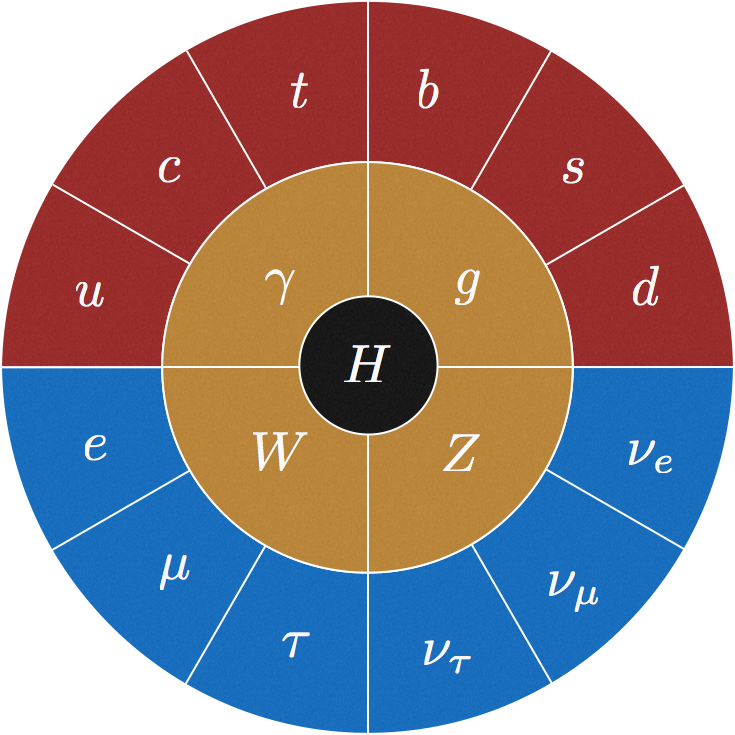
\includegraphics[width=0.8\textwidth]{images/SM-wheel.png}
  \caption{Graphical representation of the particle content of the Standard Model Source: the movie \emph{Particle Fever} (2013).}
\end{marginfigure}

However, many questions still remain unanswered by the Standard Model. For example, it does not explain why neutrinos have masses, and does not contain a viable dark matter candidate. On a more abstract level, the square of the mass of the Higgs boson seems unnaturally finely tuned - this phenomenon is termed the \emph{hierarchy problem}, and we will revisit it in \autoref{ch:supersymmetry}. In fact, it is widely believed that the Standard Model is only a low-energy effective approximation to an underlying theory that is valid at higher energy scales.

To answer these questions, we must go beyond the Standard Model with new theories. These new theories often predict new fundamental particles and forces, which we can study using particle colliders, like the Large Hadron Collider (LHC), which lies on the border between Switzerland and France (\autoref{fig:LHC_schematic}).

\begin{figure}
  \centering
  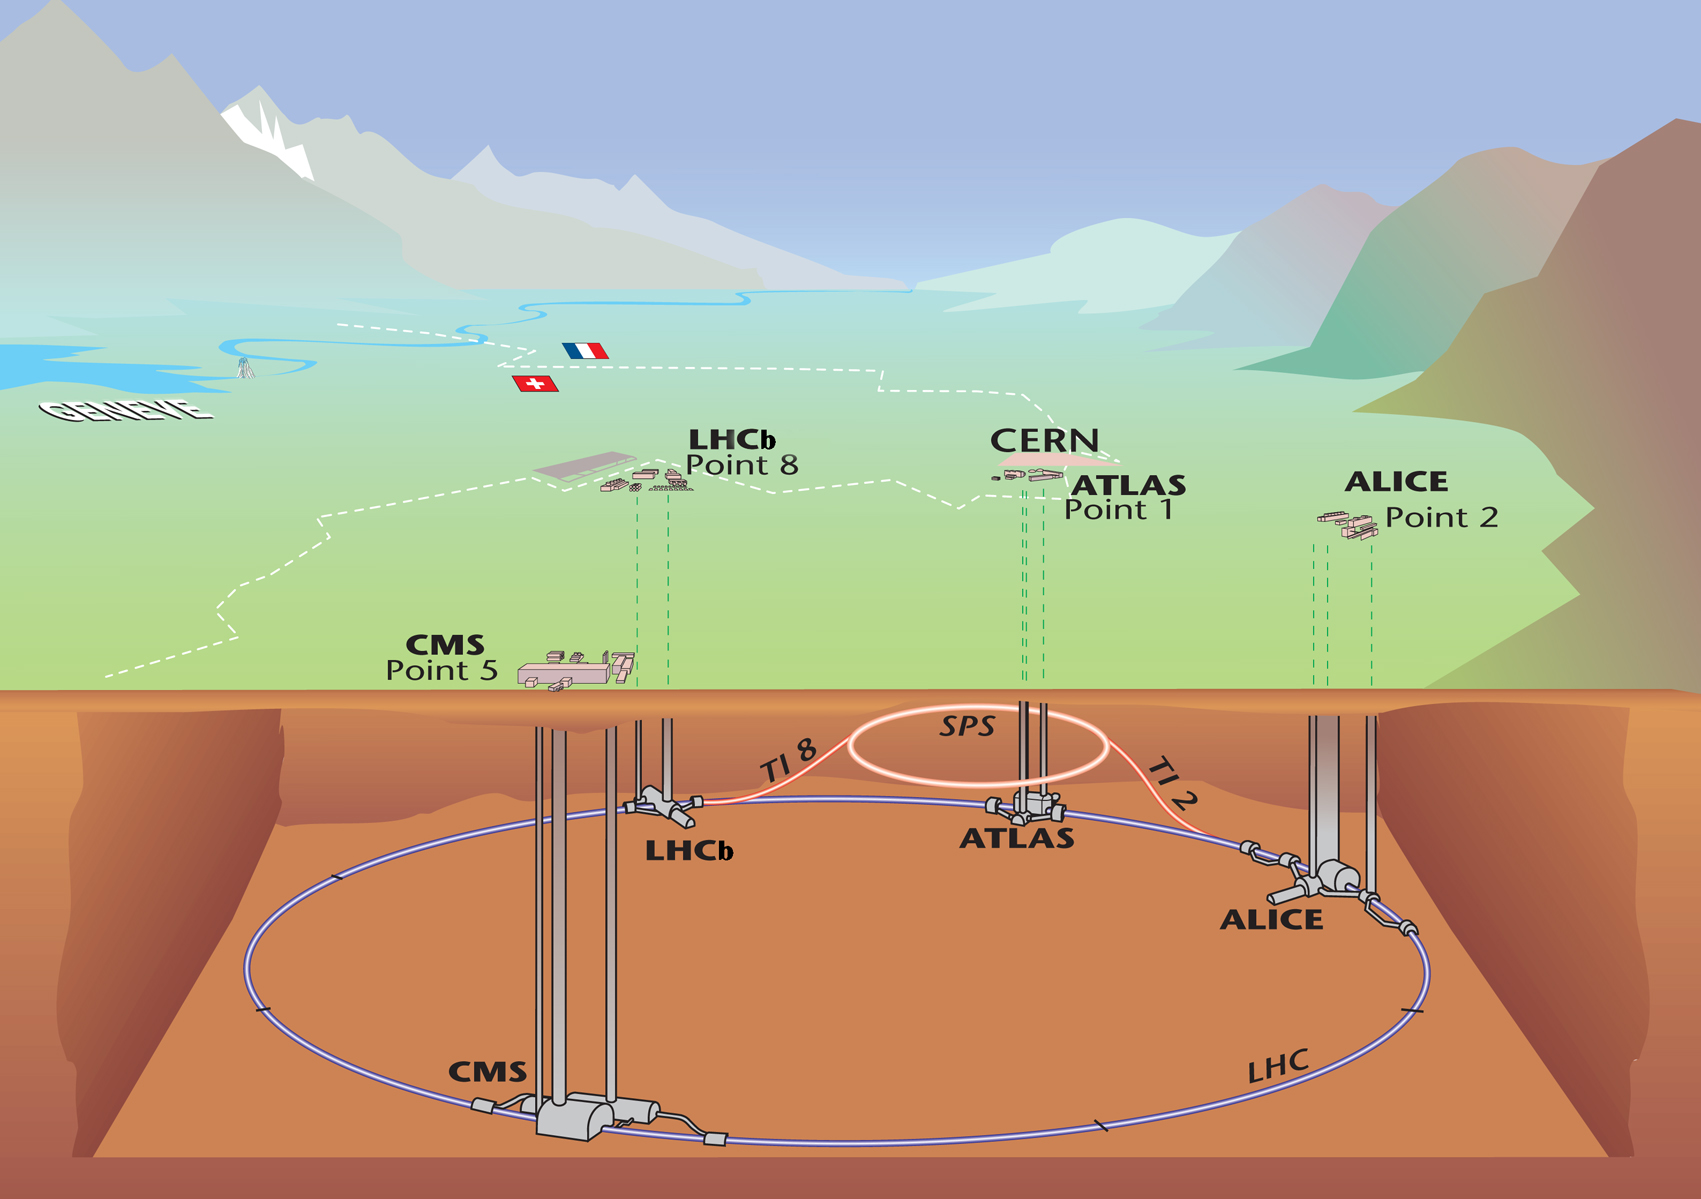
\includegraphics[width=0.9\textwidth]{images/LHC}
  \caption{Schematic diagram of the Large Hadron Collider, which lies on the border between Switzerland and France. \href{http://cds.cern.ch/journal/CERNBulletin/2008/38/News\%20Articles/1125888?ln=en}{(CERN)}}
  \label{fig:LHC_schematic}
\end{figure}

At these colliders, we collide particles at near-lightspeed, creating new particles that can be detected by extremely sophisticated detectors. One of the main challenges at particle colliders is that there are hundreds of millions of collisions every second, but only a small fraction of these will have signatures of new physics. In addition, there are a multitude of promising theories beyond the Standard Model, each possessing a large parameter space. However, performing a full experimental analysis for even a single point of this parameter space be very time consuming.

For this reason, existing theories must be constrained (or excluded entirely) by holding them up to the light of experimental evidence. Furthermore, we need to have a rough idea of what the most effective collider search strategies are before going ahead with a complete experimental analysis. This is where phenomenology steps in.

Phenomenology bridges the gap between theory and experiment - connecting the predictions of the former with the measurements of the latter. In this dissertation, we present three phenomenological analyses for finding physics beyond the Standard Model at current and future colliders. The structure of the dissertation is as follows.

\subsection{\autoref{part:Theory_and_Phenomenology}}
This part of the dissertation contains brief reviews of the Standard Model, Two Higgs Doublet Models, Minimal Supersymmetric Standard Model, and the basics of collider phenomenology and the role that machine learning can play in it. The material in these chapters is adapted from a number of review articles and textbooks that are cited in the individual chapters. Some topics are elaborated on compared to the sources, while some are condensed.  While this is not new material, it is a synthesis that the author believes provides additional context and coherence to the dissertation.
\paragraph{Chapter \ref{ch:sm}} A more or less self-contained review of the Standard Model, accessible to readers with a basic knowledge of quantum electrodynamics and group theory. It may be safely skipped by readers who are familiar with the topic. The focus of this chapter is on motivating and developing the Glashow-Weinberg-Salam theory of electroweak interactions, since the analyses in this dissertation focus on weak decays of beyond the Standard Model (BSM) particles. The treatment of this topic is semi-historical in nature. We also give an overview of the Higgs mechanism, building up to electroweak symmetry breaking through examining a few simpler examples first. We briefly touch upon asymptotic freedom and quantum chromodynamics to introduce the concept of jets at hadron colliders. Finally, we conclude by discussing a few of the limitations of the Standard Model, motivating the need to formulate new theories to address them.
\paragraph{Chapter \ref{ch:2HDMs}} This chapter motivates and reviews a class of extensions to the scalar sector of the Standard Model known as Two Higgs Doublet Models ($2$HDMs). The most general $2$HDM scalar potential is introduced and then constrained using phenomenological motivations. The mass spectrum of the extended scalar sector in such constrained models is discussed, followed by a brief listing of the Yukawa and weak interactions of these new BSM Higgs bosons. We finally conclude by pointing out the connection between Two-Higgs Doublet Models and the Minimal Supersymmetry Standard Model (MSSM) The analyses in chapters \ref{ch:LightChargedHiggs} and \ref{ch:ExoticHiggs} are designed to discover or exclude points in the parameter space of a particular kind of $2$HDM, known as the Type-II $2$HDM.
\paragraph{Chapter \ref{ch:supersymmetry}} The main motivations behind the development of supersymmetry are discussed, followed by an introduction to the algebra of supersymmetry operators. The subsequent sections introduce the concepts of superfields and superspace and review the construction of a general renormalizable supersymmetric Lagrangian. Having done this, we specialize to the Lagrangian of the MSSM, providing the superpotential, terms that softly break supersymmetry, and some phenomenologically motivated simplifying assumptions. We also list the particle content of the MSSM, grouped into chiral and gauge supermultiplets. The analysis in \autoref{ch:DM_100_TeV} is designed to explore the parameter space of the MSSM with a mass spectrum that displays a substantial hierarchy between the mass of the fermionic and scalar superpartners of SM particles.

\paragraph{Chapter \ref{ch:ColliderPheno}} This chapter describes how to connect theoretical predictions and experimental observables. The design of a generic multipurpose detector for a hadron collider is discussed, followed by discussions of some of the kinematic variables that are relevant to our analyses in \autoref{part:Three}. The concepts of hypothesis testing and statistical significance and briefly reviewed, followed by a recasting of particle physics concerns in the language of machine learning.

\subsection{\autoref{part:Three}}
In this part, we present three original collider analyses designed to probe Type-II $2$HDMs and the MSSM at the current 14 TeV LHC and a future 100 TeV hadron collider.

\paragraph{Chapter \ref{ch:LightChargedHiggs}} 
A new type of Higgs boson, known as the \emph{charged} Higgs boson $H^\pm$, arises naturally in the spectrum of $2$HDMs. Finding one of these would be an unmistakable sign of new physics beyond the Standard Model. The mass of this particle, $m_{H^\pm}$ is a free parameter in the theory. Searches for this particle can be divided into two broad categories - the first involving charged Higgs bosons lighter than the top quark, and the other dealing with charged Higgses heavier than the top quark. In this chapter, we examine the first scenario, with charged Higgses coming from the decay of top quarks that are either produced singly or in pairs. While experimental results from CMS and ATLAS  have placed a lower limit of 160 GeV for the mass of the charged Higgs boson in the context of the MSSM, these limits have been placed assuming that the charged Higgs decays solely via conventional channels to final states with SM particles. However, theories that predict charged Higgs typically predict other BSM particles as well. These can potentially be lighter than the charged Higgs, thus opening up new, `exotic' decay channels for it. For regions of parameter space with low values of the parameter $\tan\beta$, the rate of these exotic decays is much larger than the rate of the decays to SM particles, thus significantly weakening the limits set by the LHC. For a complete picture, we must take into account not only the conventional decay channels, but the exotic ones as well. In this chapter, we investigate the exotic decay of a charged Higgs to a lighter, neutral Higgs boson - either the pseudoscalar \emph{A} or the CP-even scalar \emph{H}, and a \emph{W} boson. 
We first perform a \emph{model-independent} analysis. That is, \emph{assuming} that $H^\pm$ decays exclusively to $AW^\pm/HW^\pm$, and that \emph{A/H} decays to a pair of tau leptons 8.6\% of the time, we set out to find the minimum rate of the signal process required for this analysis to discover it with a significance of 5$\sigma$, or exclude it with a significance of 1.96$\sigma$. This rate corresponds to the strength of the signal - the weaker the signal that can be probed by the analysis, the more powerful the analysis is. The model-independent limit on the signal strength can be translated into a limit on the branching ratio of the top quark to the charged Higgs, BR$(t\rightarrow H^\pm b$. We determined that the single top and the top pair channels could potentially set upper limits of 0.2\% and 0.3\% respectively on this branching ratio . For this analysis to discover the signal process, the branching ratio would have to be about three times higher than the aforementioned upper limits. These results can be translated into contours in the two-dimensional $m_{H^\pm}-\tan\beta$ plane in the parameter space of a Type-II $2$HDM that delineate regions that can be either discovered or excluded with this analysis. We also found that this analysis would be able to discover points with the charged Higgs mass $m_{H^\pm}$ between 155 and 165 GeV for $\tan\beta >$17, and the entire viable mass range for $\tan\beta <$6. We also found that almost the entire relevant region of the $m_{H^\pm}-\tan\beta$ plane can be excluded with this analysis, with the exception of the regions with very small mass differences between the charged Higgs and the top quark. In summary, we found that the exotic decay channel $H^\pm\rightarrow AW^\pm/HW^\pm$ probes a region of parameter space complementary to the region probed by standard decay channels (such as $H^\pm\rightarrow \tau\nu$), and is thus an important search channel to include in the search for charged Higgs bosons.
The results in this chapter have been published as an article in the Journal of High Energy Physics \citep{Kling2015c}, co-authored with Felix Kling and Shufang Su. While there has been some editing to achieve integration with the dissertation, there will inevitably be a substantial overlap between the chapter and the published article. The collider analysis for the top pair production channel, as well as the calculation of the limits was carried out by Felix, while analysis for the single top production channel was performed by the author of this dissertation.  

\paragraph{Chapter \ref{ch:ExoticHiggs}}
While the project that \autoref{ch:LightChargedHiggs} is based on dealt with the implications of additional, exotic decay channels opening up for charged Higgs bosons arising from extended scalar sectors at the LHC, the project that this chapter is based on is much more ambitious in scope, aiming for nothing less than a complete prospectus of exotic Higgs decay channels in $2$HDMs with large mass hierarchies. The authors of \citep{Kling2016} have presented a collection of promising $2$HDM benchmark planes for investigation at the LHC that take into account theoretical and experimental constraints, and highlight the complementarity between the different search channels. The end goal of this project is to perform detailed collider analyses to determine exclusion and discovery bounds for both the original benchmark planes at the 14 TeV LHC, as well as extended versions of them at a 100 TeV collider that, reflecting the higher obtainable mass reach. In this chapter, we present preliminary results based on collider analyses carried out for two of the benchmark planes, corresponding to the mass hierarchies $m_H < m_A = m_{H^\pm}$ and $m_A < m_H = m_{H^\pm}$. The exotic decay channels considered are $A\rightarrow HZ$ and $H^\pm\rightarrow HW^\pm$. As already shown in \autoref{ch:DM_100_TeV}, machine learning techniques represent a substantial improvement over rectangular selection cuts. Taking this and the extremely large number of benchmark points we need to scan across into account, the analyses in this chapter are based solely on boosted decision tree classifiers. Using this technique, we are able to exclude charged Higgses with masses up to 2 TeV, for neutral Higgses \emph{H} with masses up to 500 GeV, in the benchmark plane IIB suggested in \cite{Kling2016} through the decay mode $H^\pm\rightarrow AW^\pm$ at a 100 TeV collider.

This work is being done in collaboration with Felix Kling, Huayang Song, Honglei Li, and Shufang Su. The results for the $A\rightarrow HZ$ channels have been obtained by Huayang and Honglei by using and extending analysis code originally written by Felix, while the results for the $H^\pm\rightarrow HW^\pm$ decay channel have been obtained by the author using code that builds upon that used for \autoref{ch:DM_100_TeV}. The Monte Carlo event samples for all the channels at 100 TeV were generated by the author on the University of Arizona computing cluster.

\paragraph{Chapter \ref{ch:DM_100_TeV}}
A 100 TeV proton-proton collider will be an extremely effective way to probe the electroweak sector of the Minimal Supersymmetric Standard Model (MSSM). In this chapter, we describe a search strategy for discovering pair-produced higgsino\footnote{Higgsinos are the fermionic counterparts of scalar Higgs fields. The title of the dissertation is thus potentially a generous interpretation of the term `Higgses' - but the alliteration was just too good to pass up.}-like neutralinos $\tilde{\chi}_{2,3}^0$ that decay to the lightest neutralino $\tilde{\chi}_1^0$ (which we assume to be an almost pure bino). We investigate the particular case in which the higgsinos decay via intermediate \emph{Z} and SM Higgs bosons \emph{h}, that in turn decay to a pair of leptons and a pair of \emph{b}-quarks respectively: 
$$\tilde{\chi}^0_{2,3}\tilde{\chi}^0_{3,2}\rightarrow (Z\tilde{\chi}^0)(h\tilde{\chi}_1^0)\rightarrow bbll+\tilde{\chi}_1^0\tilde{\chi}_1^0.$$
We performed two analyses simultaneously - the first using rectangular selection cuts on physically motivated kinematic observables known as razor variables, and the second using the same high-level observables, along with a few lower-level observables as input features for a Boosted Decision Tree Classifier. The results show that the machine learning technique performs substantially better than the regular rectangular selection cuts. With the machine learning analysis, we would be able to discover higgsinos up to a mass of 1.3 TeV, and exclude them to up to a mass of 1.8 TeV. Correspondingly, we can discover binos up to 900 GeV, and exclude them up to 1.3 TeV. The research for this chapter was carried out by the author under the guidance of Shufang Su, and forms the basis of a completed manuscript that will soon be submitted for publication in a peer-reviewed journal.

Finally, we conclude in \autoref{ch:Conclusion}, where we provide a summary of our findings and discuss prospects for future work.

%Generating these samples for hundreds of signal benchmark points and backgrounds with extremely large cross sections is not a trivial task (and even less so at 100 TeV), and requires careful management of computational resources. During the course of performing the research that comprises this dissertation, the author has developed a Python-based framework, \texttt{clusterpheno}, for event generation and analysis on a cluster. An advantage of using this over the CMS gridpack method is that the entire pipeline of MadGraph-Pythia-Delphes is integrated

\chapter{The Standard Model and Beyond}\label{ch:theory}

\newcommand{\ct}{\cos\theta_w}
\newcommand{\st}{\sin\theta_w}

In this chapter, we will provide some of the theoretical background that our research builds upon. We will first provide a lightning-quick review of the particle content and gauge structure of the Standard Model, followed by an introduction to Two-Higgs Doublet Models and the Minimal Supersymmetric Standard Model. For excellent treatments of the Standard Model, please see \citep{Cheng:1984,Schwartz:2014,Zee:2003mt,Peskin:1995ev}. For a detailed review of Two-Higgs Doublet Models, see  \cite{Branco:2011iw}, and for a pedagogical introduction to supersymmetry and the MSSM, see \cite{Martin:1997ns}. Our discussion is adapted from these works. 

\section{The Standard Model}\label{sec:sm}

The fundamental constituents of matter are fermions. The interactions between these fermions are mediated by particles known as \emph{gauge bosons}, which arise from the gauge structure of the Standard Model:
\[SU(3)\times SU(2)\times U(1)_Y\]
This means that each fermion transforms in a unique way under transformations corresponding to these gauge groups. In addition to the fermions and gauge bosons, the standard model contains a scalar $SU(2)$ doublet \emph{H}, known as the Higgs field. In \autoref{tab:SM_fields}, we collect the fundamental fields of the SM and their transformation properties under different gauge groups. The labels \emph{u,d,e} and $\nu$ are collective labels for three generations of fermions, shown in \autoref{tab:fermion_generations}. The fields \emph{g}, $W_\mu$, and $B_\mu$ are vector bosons that that correspond to the $SU(3)$, $SU(2)$ and $U(1)$ gauge group respectively.

\begin{table}
  \begin{sidecaption}{The fields of the Standard Model, grouped by their charges under the relevant gauge groups.}[tab:SM_fields]
  \[
  \begin{array}{lccccc}
    \toprule
   \text{Type}                & \text{Field}              & \text{Spin}      & SU(3)      & SU(2)      & U(1)_Y \\\midrule
   \text{Scalar}              & H                         & 0                & \mathbf{1} & \mathbf{2} & \slantfrac{1}{2}\\\midrule
   \text{Fermions}            & Q = \vdoublet{u_L}{d_L}   & \slantfrac{1}{2} & \mathbf{3} & \mathbf{2} & \slantfrac{1}{6}\\
                              & u_R                       &                  & \mathbf{3} & \mathbf{1} & \slantfrac{2}{3}\\
                              & d_R                       &                  & \mathbf{3} & \mathbf{1} & -\slantfrac{1}{3}\\
                              & L = \vdoublet{e_L}{\nu_L} &                  & \mathbf{1} & \mathbf{2} & -\slantfrac{1}{2}\\
                              & e_R                       &                  & \mathbf{1} & \mathbf{1} & -1\\\midrule
    \text{Vector bosons}      & g                         & 1                & \mathbf{8} & \mathbf{1} & 0 \\
                              & W_\mu                     &                  & \mathbf{1} & \mathbf{3} & 0 \\
                              & B_\mu                     &                  & \mathbf{1} & \mathbf{1} & 0\\
    \bottomrule
  \end{array}
\]
\end{sidecaption}
\end{table}

The ground state that we inhabit spontaneously breaks the larger symmetry $SU(2)\times U(1)_Y$ to the symmetry $U(1)_\text{EM}$. The subscript \emph{Y} denotes the hypercharge of the field, while the subscript EM denotes electromagnetism. In this process (which we will revisit in more detail in \autoref{subsec:ewsb}), the three gauge fields $W_\mu$, corresponding to the $SU(2)$ gauge symmetry, combine with the $B_\mu$ field corresponding to the $U(1)_Y$ symmetry to form the massive gauge bosons $W^\pm$ and $Z$, and a massless photon, $A_\mu$ (often denoted by $\gamma$ instead). The \emph{W} and \emph{Z} bosons mediate the weak interactions that responsible to phenomena such as radioactive decay, while the photon mediates electromagnetic interactions. The gauge field \emph{g} corresponding to the $SU(3)$ gauge symmetry is known as the \emph{gluon}, and mediates the strong force between nucleons. 


\begin{table}
  \raggedright
\strictpagecheck
\begin{adjustwidth*}{0in}{-0.5in}
  \begin{tabular}{cllll}
    \toprule
    Generation & \multicolumn{2}{c}{Quarks} & $e$: Leptons & $\nu$: Neutrinos \\ \cmidrule(r){2-3}
     & $u$: Up & $d$: Down &                                       & \\\midrule
    I           & $u:$ up                    & $d:$ down     & $e:$ electron                         & $\nu_e:$ electron neutrino\\
    II          & $c:$ charm                 & $s:$ strange  & $\mu:$ muon                           & $\nu_\mu:$ muon neutrino\\
    III         & $t:$ top                   & $b:$ bottom   & $\tau:$ tau                           & $\nu_\tau:$ tau neutrino\\
    \bottomrule
  \end{tabular}
  \caption{The fermion sector of the Standard Model, grouped by generation.}
  \label{tab:fermion_generations}
\end{adjustwidth*}
\end{table}
\subsection{Electroweak symmetry breaking}\label{subsec:ewsb}
In 1957, Schwinger proposed the unification of the weak and electromagnetic interactions, citing their vectorial nature. In 1961, Glashow proposed a model for weak interactions governed by symmetry under the product group $SU(2)\times U(1)$. The trouble was, experiments had shown that the weak interactions had a short range, implying that the vector bosons that mediated them must be massive. On the other hand, gauge symmetry prohibits mass terms for these intermediate vector bosons. Glashow's theory included these mass terms, but they were put in by hand, and spoiled the renormalizability of the theory. A possible way out was to break the gauge symmetry \emph{spontaneously} rather than explicitly. Spontaneous symmetry breaking refers to the phenomenon where the ground state of a system does not respect the symmetry of the full Lagrangian. However, Goldstone's theorem states that for every spontaneously broken symmetry, there exists a set of massless spin-0 bosons corresponding to the generators of the symmetry group - since such particles have never been observed, this was obviously an undesirable feature of the theory. 

Thus we seem to have to choose between two undesirable outcomes: a set of massless gauge bosons, or a set of massless scalars, both of which are inconsistent with what we actually see in nature. Remarkably, each of these problems would turn out to be the solution for the other, through the marvelous \emph{Higgs mechanism}. This mechanism was first put forth by Philip W. Anderson in the context of condensed matter systems. In 1964, three groups -- Peter Higgs, the duo of Francois Englert and Robert Brout, and the trio of Gerald Guralnik, C. R. Hagen, and Tom Kibble -- independently and almost simultaneously proposed that this mechanism could explain how the the weak interaction mediators can acquire mass. There is likely a strong case for naming the mechanism after all of these physicists, but for the sake of expediency, we will simply refer to it as the Higgs mechanism.

The Higgs mechanism describes the spontaneous breaking of electroweak symmetry, that is, the breakdown of the product group $SU(2)\times U(1)_Y\rightarrow U(1)_{EM}$. This is achieved by adding to the theory a complex scalar $SU(2)$ doublet, the Higgs field $H$:
\[H = \vdoublet{H^+}{H^0}.\]
The terms of the Lagrangian that involve this field can be written as follows:
\begin{align}
  \label{eq:higgs_kinetic}
  \mathcal{L}_{\text{Higgs}} &= \frac{1}{2}\left|D_\mu H\right|^2-V(H)\\
  \label{eq:higgs_potential}
  \text{where }V(H) &= \left(H^\dag H-\frac{v^2}{2}\right)^2
\end{align}
The gauge covariant derivative for the Standard Model takes the form (neglecting the term corresponding to the unbroken $SU(3)$ symmetry)
$$D_\mu = \partial_\mu + igW_\mu^aT^a+ig'YB_\mu,$$
where $W_\mu^a$ and $B_\mu$ are the gauge fields corresponding to the $SU(2)$ and $U(1)_Y$ symmetries respectively, \emph{g} and $g'$ are coupling constants, and $T^a$ and $Y$ are the generators of the $SU(2)$ and $U(1)$ groups. The potential $V(H)$ reaches its minimum when $H^\dag H = v^2 / 2$. We pick a non-zero vacuum expectation value (VEV) for $H$ that breaks the neutral sector symmetry (corresponding to $H^0$) but not the charged symmetry (corresponding to $H^{+}$), since we wish to keep photons massless. This VEV is given by:
\[H = \vdoublet{0}{\frac{v}{\sqrt{2}}}.\]
Plugging this into the kinetic term of the Lagrangian, and isolating the terms quadratic in the gauge fields, we get
\[\frac{g^2v^2}{4}W_\mu^-W_\mu^++\frac{1}{2}\frac{v^2}{4}(g^2+g'^2)
\left(\ct W_\mu^3 - \st B_\mu\right)^2\]
where $W_\mu^\pm = (W_\mu^1\pm iW_\mu^2)/\sqrt{2}$  and $\theta_w = \tan^{-1}(g'/g)$ is the \emph{Weinberg angle}, which parameterizes the mixing between the photon $A_\mu$ and the $Z$ boson $Z_\mu$.
\begin{equation}\label{eq:z_a_mixing}
\vdoublet{Z_\mu}{A_\mu} = \fourmatrix{\ct}{-\st}{\st}{\ct}
\vdoublet{W_{\mu}^{3}}{B_{\mu}}
\end{equation}
The product $W_\mu^+W_\mu^-$ can be interpreted as a mass term for a charged vector boson, $W_\mu^\pm$. Collecting the terms quadratic in $W_\mu^\pm$ and $Z_\mu$, we get
\[\mathcal{L}_{\text{mass terms}}=\frac{e^2v^2}{4\sin^2\theta_w}W_\mu W^\mu+
\frac{e^2v^2}{8\sin^2\theta_w\cos^2\theta_w}Z_\mu Z^\mu.\]
Thus, after accounting for symmetry factors, we get the masses of the \emph{W} and \emph{Z} bosons as:
\begin{align*}
  m_W &=\frac{ev}{2\st}, & 
  m_Z &=\frac{ev}{\sin2\theta_w}.
\end{align*}
We see that there is no mass term for $A_\mu$. Thus the \emph{W} and \emph{Z} bosons gain mass, limiting their range, while the photon remains massless, corresponding to what is experimentally observed. Remarkably, we have done this without violating gauge invariance. Colloquially, we say that the \emph{W} and \emph{Z} bosons have `eaten' the Goldstone boson degrees of freedom to obtain mass. 

Peter Higgs was the first to postulate the existence of a physical scalar particle that could be produced by perturbing the vacuum. To see how this plays out, let us parameterize the Higgs doublet field as 
\[H = \frac{1}{\sqrt{2}}\exp\left(i\xi^a(x)\frac{\tau^a}{v}\right)\vdoublet{0}{v + h(x)}.\]
where $\tau^a$ are the Pauli matrices, $\xi^a$ and $h$ are scalar fields with VEVs given by $\langle\xi\rangle=\langle h\rangle=0$, and \emph{v} is the vacuum expectation value of the Higgs doublet, experimentally measured to be about 246 GeV. The field $h$ is known as the \emph{Higgs boson}. The simplest gauge choice to examine this scenario is the unitary gauge, where $\xi(x)=0$. In this gauge, the potential $V(H)$ from \eqref{eq:higgs_potential} becomes:
\[V(H) = -\frac{1}{2}m_h^2 h^2 - \lambda vh^3 -\frac{1}{4}\lambda h^4\]
The Higgs boson is the only fundamental scalar in the Standard Model, and was discovered in 2012, nearly 50 years after it was first predicted. The coefficient of the term quadratic in $h$ is its mass, $m_h$ - a free parameter that had to be determined experimentally. The second and third terms in the above expression represent the trilinear and and quartic self-coupling of the Higgs boson.
\subsection{Quark mass and gauge eigenstates}
While the quarks listed in \autoref{tab:fermion_generations} are \emph{gauge eigenstates}, with well defined transformations under the gauge groups, the physical states that we observe at a collider will in fact be \emph{mass eigenstates}. The two are related by the \emph{Cabibbo-Kobayashi-Maskawa} (\textsc{ckm}) matrix:
\sidepar{The Cabibbo-Kobayashi-Maskawa quark mixing matrix}
\begin{equation}
  V_\text{CKM} =
  \begin{pmatrix}
    V_{ud} & V_{us} & V_{ub}\\
    V_{cd} & V_{cs} & V_{cb}\\
    V_{td} & V_{ts} & V_{tb}
  \end{pmatrix}
\end{equation}
The elements of the matrix denote the level of mixing between the gauge eigenstates. Experimentally, this matrix has been determined to be nearly diagonal.

\subsection{Asymptotic freedom and QCD}

In the 50s and 60s, experiments were devised to unravel the structure of the proton. They found two seemingly incompatible results. On the one hand, colliding protons resulted in the production of a large number of pions collinear with the beam axis, implying that the protons could not absorb a large momentum transfer. However, deep inelastic scattering experiments later showed that it was possible for an energetic electron to undergo hard electromagnetic scattering off a proton. These disparate phenomena were reconciled by the introduction of the \emph{parton model} by Bjorken and Feynman. In this model, hadrons such as the proton were comprised of a collection of loosely bound pieces, known as partons (for an artistic representation, see \autoref{fig:proton_innards}). To an energetic incoming electron, these partons would appear approximately free, allowing it to scatter with a large momentum transfer off of one of them. The struck parton will then exchange momentum softly via the strong interaction among the other partons, which results in the production of a \emph{jet} of hadrons, collinear with the direction of the original struck parton. The deeper reason for this behavior is that these partons are charged under a non-Abelian gauge group, $SU(3)$. The phenomenon of the weakening of the interaction strength at large momentum transfers is known as \emph{asymptotic freedom}, and it is a property of non-Abelian gauge theories.
\begin{marginfigure}[-3in]
  \strictpagecheck
  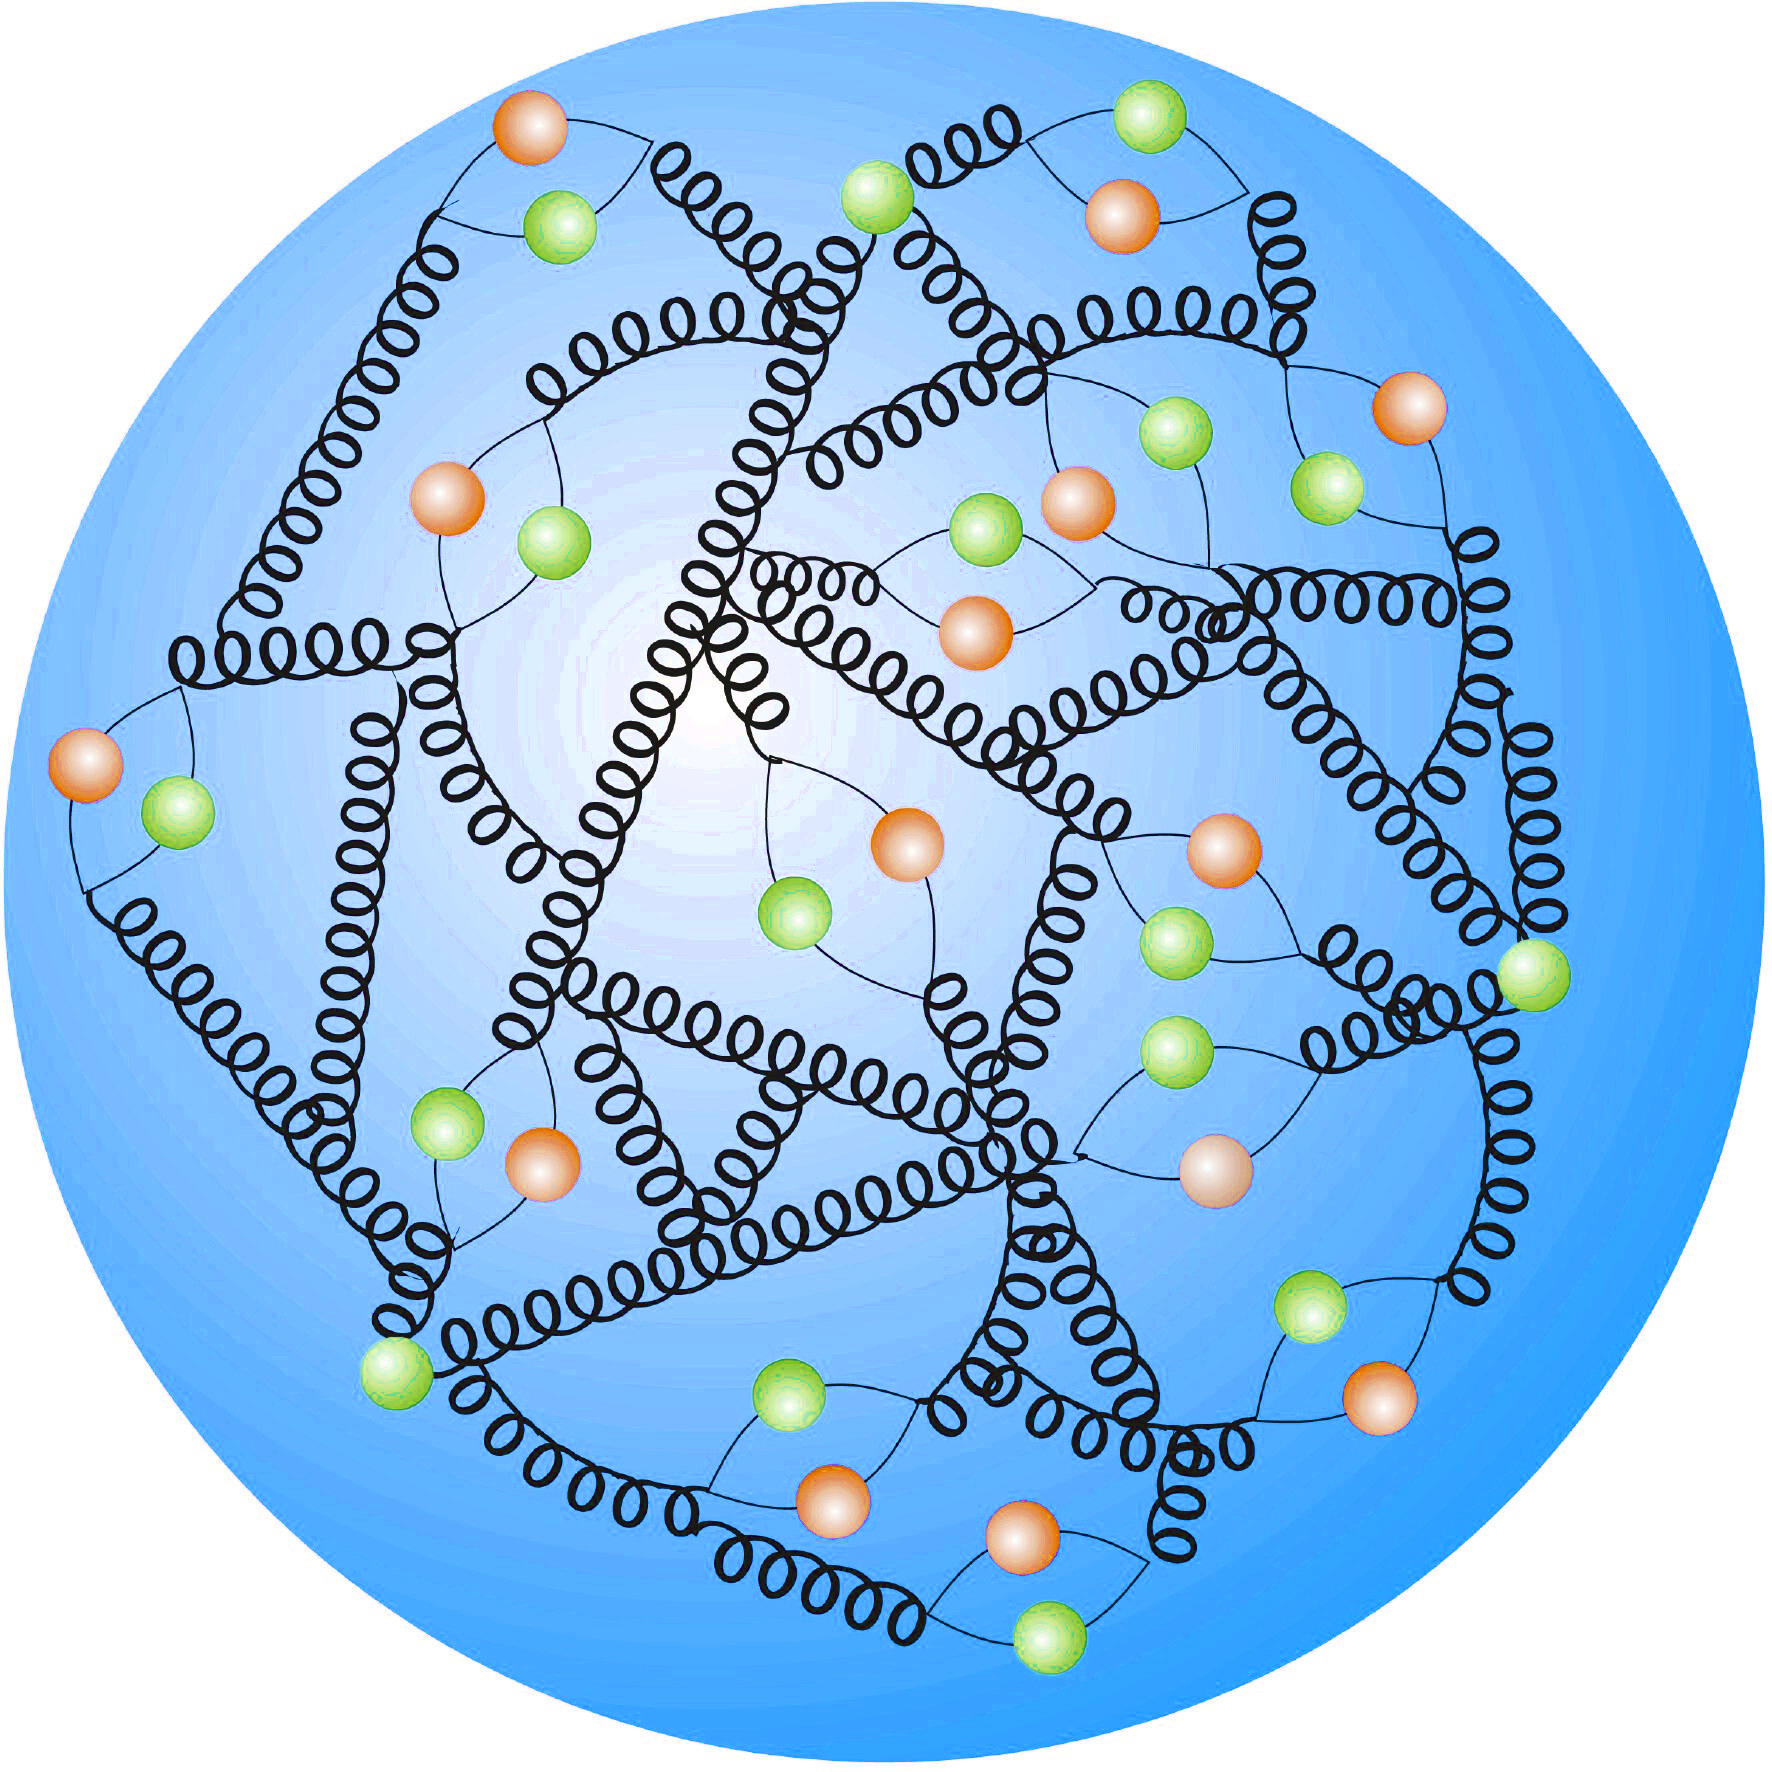
\includegraphics[width=0.8\textwidth]{images/proton_innards}
\caption{A representation of the innards of a proton, showing the dynamic structure. Source: \citep{proton_structure}}
\label{fig:proton_innards}
\end{marginfigure}
The $\beta$-function of a gauge theory describes the evolution of the renormalized coupling constant with energy. For non-Abelian gauge theories, it takes the following form (up to leading order):%
\sidepar{Leading order $\beta$-function for non-Abelian gauge theories}
\begin{equation}
  \beta(g_R) = \mu\frac{d}{d\mu}g_R = -\frac{g_R^3}{(4\pi)^2}\left[\frac{11}{3}C_A -\frac{4}{3}n_fT_F\right]
\end{equation}
where $\mu$ is the renormalization scale, $C_A$ is the quadratic Casimir operator for the adjoint representation, and $T_F$ is the \emph{index} of the fundamental representation.
In the case of the strong interaction, the relevant gauge group is $SU(3)$. Thus $C_A = 3$ and $T_F = \frac{1}{2}$. If $n_f$, the number of quark flavors is less than 17 \footnote{Which it is, since the number of quark flavors is six, as can be seen in \autoref{tab:fermion_generations}.}, the $\beta$ function has a \emph{negative} sign, which means that the coupling \emph{decreases} at higher energies. This is the underlying basis of asymptotic freedom. The theory of the strong interaction is known as \emph{quantum chromodynamics}, or QCD for short. The analogue of electric charge for this theory is a quantity referred to as \emph{color} (hence the name of the theory). At a hadron collider, it is of crucial importance to understand the physics of gluons and jets.

The Standard Model of particle physics has been remarkably successful, and over the decades has yielded some of the most precise measurements in all of physics. However, as mentioned in \autoref{ch:introduction}, there still remain unresolved issues with it. In the next two sections we will discuss some of these issues in more depth, and introduce extensions to the SM that potentially resolve them.

\section{Two-Higgs Doublet Models}\label{sec:2HDMs}

Intuitively, it is not too hard to imagine, based on the complex structure of the fermion and gauge sectors of the Standard Model, that its scalar sector might well contain members other than a single $SU(2)$ doublet. An extended scalar sector frequently arises in BSM theories that potentially alleviate some of the unresolved issues facing the Standard Model.
% Strong CP problem
One of these issues is the \emph{strong CP problem}, which can be summarized as follows. Lagrangians for Yang-Mills theories can have a renormalizable term that is gauge-invariant but violates CP, of the form
\[\mathcal{L}_{\theta} = \theta\epsilon^{\mu\nu\alpha\beta}F_{\mu\nu}^aF_{\alpha\beta}^a,\]
where $\theta$ is some angle, $F_{\mu\nu}^a$ are the field strength tensors, and $\epsilon^{\mu\nu\alpha\beta}$ is an antisymmetric tensor. This term is a total derivative, since it can be written as $2\theta\partial_\mu(\epsilon^{\mu\nu\alpha\beta}A_\nu^aF_{\alpha\beta}^a)$. Thus, it should not contribute to perturbative effects. However, this term can potentially contribute to non-perturbative effects. Additionally, this term can be modified be chiral rotations of the form $\psi\rightarrow \exp(i\gamma_5\theta_F)\psi$. Since physical observables should be independent of the choice of the basis, i.e. $\theta_F$, we should absorb it into $\theta$ by defining a basis-independent phase: $\bar{\theta} = \theta-\theta_F$. For $SU(2)$ and $U(1)$ gauge symmetries, this phase can be set to zero by performing appropriate chiral rotations of the fermion fields. However, no such choice exists for the term corresponding to the the $SU(3)$ group, and thus the CP-violating term in the QCD Lagrangian could in principle by non-zero. A non-zero value of $\bar{\theta}$ would be manifested as non-perturbative effects. For example, the neutron would then have a non-zero electric dipole moment. However, experiments have shown that $\bar{\theta}$ must be vanishingly small, with a stringent upper bound: $\bar{\theta}<10^{-10}$. A value this small seems suspiciously \emph{fine-tuned} in the absence of an underlying symmetry to enforce it.

Adding an additional scalar doublet allows us to impose such a symmetry - a global $U(1)$ symmetry known as \emph{Peccei-Quinn} symmetry. If this symmetry is spontaneously broken, a Goldstone boson arises, which can then be chirally rotated such that $\bar{\theta}$ becomes effectively zero for the ground state.
% Baryon asymmetry
Extended scalar sectors also arise in theories that can explain the observed imbalance between matter and antimatter in the universe. The CP violation in the weak sector of the Standard Model cannot account for this imbalance, but $2$HDMs, with their complex scalar sector and possible new sources of CP violation, can.
%
However, the strongest motivation for $2$HDMs is their connection to supersymmetric models that have the potential to resolve the hierarchy problem, discussed in the next section. The scalar sector of the Minimal Supersymmetric Standard Model  has a structure similar to that of a $2$HDM - it requires exactly two scalar doublets to give mass to both up and down type fermions, and for the cancellation of anomalies. With these motivations for $2$HDMs in mind, let us examine the structure of the scalar potential of a generic Two-Higgs Doublet Model.

\subsection{The $2$HDM scalar potential}
The most general renormalizable scalar potential for two scalar doublets $\Phi_1$ and $\Phi_2$ with hypercharge $+1$ is given by
\strictpagecheck
\sidepar{Scalar potential for a Two-Higgs Doublet Model}
\begin{align}
\label{eq:2HDM_scalar_potential}
  \begin{split}
  V(\Phi_1,\Phi_2) &= m_{11}^2|\Phi_1|^2 + m_{22}^2|\Phi_2|^2 - m_{12}^2\left(\Phi_1^\dagger\Phi_2 + \text{h.c.}\right)\\
&+\frac{\lambda_1}{2}|\Phi_1|^4 + \frac{\lambda_2}{2}|\Phi_2|^4+\lambda_3|\Phi_1|^2|\Phi_2|^2 + \lambda_4|\Phi_1^\dagger\Phi_2|^2\\
&+\left[\frac{\lambda_5}{2}\left(\Phi_1^\dagger\Phi_2 \right)^2+\lambda_6|\Phi_1|^2(\Phi_1^\dagger\Phi_2)+\lambda_7|\Phi_2|^2(\Phi_1^\dagger\Phi_2) + \text{h.c.}\right]
\end{split}
\end{align}
where h.c. stands for the hermitian conjugate of the terms immediately preceding it. The parameters $m_{11,22}^2$ and $\lambda_{1,2,3,4}$ are real while the parameters $m_{12}^2$ and $\lambda_{5,6,7}$ can be complex. Naively, it would seem that this potential has 14 degrees of freedom - six from the real parameters, and eight from the complex parameters. However, it should be noted that we have the freedom to perform basis transformations, that is, we can write the potential in terms of new doublets $\Phi_a' = \sum_{b=1}^2U_{ab}\Phi_b$. where $U_{ab}$ is a 2$\times$2 unitary matrix. The condition of unitarity implies that $U$ has three degrees of freedom, which can absorb three out of the 14 degrees of freedom listed earlier. Thus, only 11 out of the original 14 degrees of freedom are physical.

In principle, we could proceed with these 11 parameters, however, there are a couple of reasons to attempt to reduce this number. The first is that a large number of free parameters makes a theory less falsifiable, thus reducing its predictive power. The second is that in order to distinguish between pseudoscalars and scalars, CP must be conserved in the Higgs sector. Finally, the potential in \eqref{eq:2HDM_scalar_potential} allows for tree-level flavor-changing neutral currents (FCNC), which are experimentally measured to be highly suppressed. These can be eliminated by introducing discrete or continuous symmetries. Imposing a discrete symmetry such as $\mathcal{Z}_2$\footnote{That is, the Lagrangian is invariant under the reflection of one of the doublets: \[\Phi_i\rightarrow-\Phi_i\].} removes the terms that are odd in $\Phi_i$. This effectively sets $\lambda_6=\lambda_7 = 0$. In principle, this should set $m_{12} = 0$ as well, but we retain this term since it breaks the $\mathcal{Z}_2$ symmetry softly, relaxing the experimental bounds on the mass spectrum.
After imposing these constraints, all the remaining parameters $\lambda_{1,2,3,4,5}, m_{11,12,22}^2$ are real. From here on, we will only consider $2$HDMs with these constraints. 

There are four such models, classified based on the coupling patterns of the fermions to the two Higgs doublets. In Type I $2$HDMs, all the quarks couple to only one of the Higgs doublets, chosen by convention to be $\Phi_2$. In Type II $2$HDMs, the up-type right-handed quarks (\emph{u,c,t}) couple to $\Phi_2$, and the down-type right-handed quarks (\emph{d,s,b}) couple to $\Phi_1$. In both of these models, the right-handed leptons couple to the same doublet as the down-type quarks. The lepton-specific model is similar to the Type I model, except in this case, the right-handed leptons couple to $\Phi_1$. Similarly, the `flipped' model is similar to the Type II $2$HDM, except that the leptons couple to $\Phi_2$. The coupling patterns for these models are collected in \autoref{tab:no_FCNC_$2$HDMs}.
\begin{margintable}[0.5cm]
\small{
  \begin{tabular}{lccc}
	\toprule
    Model & $u_R^i$ & $d_R^i$  & $e_R^i$\\
    \midrule
    Type I          & $\Phi_2$ & $\Phi_2$ & $\Phi_2$\\
    Type II         & $\Phi_2$ & $\Phi_1$ & $\Phi_1$\\
    Lepton-specific & $\Phi_2$ & $\Phi_2$ & $\Phi_1$\\
    Flipped         & $\Phi_2$ & $\Phi_1$ & $\Phi_2$\\
    \bottomrule
  \end{tabular}}
  \caption{Fermion coupling patterns for $2$HDMs with flavor conservation.}
  \label{tab:no_FCNC_$2$HDMs}
\end{margintable}
\noindent The scalar potential $V(\Phi_1,\Phi_2)$ is minimized for non-zero vacuum expectation values of $\Phi_i$:
\begin{align}
\langle\Phi_i\rangle_0=\vdoublet{0}{\frac{v_i}{\sqrt{2}}}.
\end{align}
where $v_i$ are the vacuum expectation values of the doublets $\Phi_i$. These doublets can then be written as follows:
\begin{equation}\label{eq:2HDM_doublet_components}
\Phi_i = \vdoublet{\phi_i^+}{\frac{1}{\sqrt{2}}(v_i+\rho_i+i\eta_i)}
\end{equation}
where $\phi_i^+$ are complex charged scalars, and $\rho_i$ and $\eta_i$ represent the real and complex degrees of freedom of the neutral components of the doublets. The two doublets, each with two complex components, embody eight degrees of freedom in total. 
The process of electroweak symmetry breaking causes three of these degrees of freedom to be `eaten' by the \emph{W} and \emph{Z} bosons, and the remaining five are manifested as physical scalar fields. These consist of a pair of CP-even neutral scalars \emph{h} and \emph{H}, a CP-odd pseudoscalar \emph{A}, and a charged scalar $H^\pm$.

\subsection{The $2$HDM mass spectrum}

In this section, we will analyze the mass spectrum of flavor-conserving $2$HDMs. To do so, we construct the mass matrices by taking derivatives of the scalar potential
\[M_{ij} = \frac{\partial V(\Phi_1,\Phi_2)}{\partial\phi_i\partial\phi_j},\]
where $\phi_{i}$ can be any of the fields $\phi_i^+,\rho_i,\eta_i$ in \eqref{eq:2HDM_doublet_components}. 
Applying this procedure to the charged scalar components $\phi_i^\pm$, we obtain their mass matrix $M_{\phi^{\pm}}$:
\[M_{\phi^\pm} = \left[m_{12}^2-(\lambda_4+\lambda_5)v_1v_2\right]\fourmatrix{v_2/v_1}{-1}{-1}{v_1/v_2}.\]
Diagonalizing this matrix gives us the mass of the charged Higgses:
\[m_{H^\pm}^2 = (v_1^2+v_2^2)\left[m_{12}^2/v_1v_2-(\lambda_4+\lambda_5)\right].\]
Similarly, the mass matrix for the pseudoscalars is given by
\[M_{\eta} = \frac{m_A^2}{v_1^2+v_2^2}\fourmatrix{v_2^2}{-v_1v_2}{-v_1v_2}{v_1^2}.\]
Diagonalizing it gives us a massless Goldstone boson $G^0$, corresponding to a zero eigenvalue, and a pseudoscalar Higgs boson $A$, with mass given by
\[m_A^2 = (v_1^2+v_2^2)\left[m_{12}^2/v_1v_2-2\lambda_5\right].\]
The diagonalization process amounts to a rotation of the basis vectors by some angle. For the CP-odd and the charged scalars, this angle is the same, and is denoted as $\beta$. Given that the couplings of the Higgs bosons in $2$HDMs depend on this angle and the angle $\alpha$ \eqref{eq:alpha_def}, let us adopt the notation 
\[s_\theta,c_\theta,t_\theta = \sin\theta,\cos\theta,\tan\theta\]
for brevity. In this notation, the mass eigenstates are given by
\begin{align}
\vdoublet{A}{G^0} = \fourmatrix{s_\beta}{-c_\beta}{c_\beta}{s_\beta}\vdoublet{\eta_1}{\eta_2}&&\text{and}&&
\vdoublet{H^\pm}{G^\pm} = \fourmatrix{s_\beta}{-c_\beta}{c_\beta}{s_\beta}\vdoublet{\phi_1^+}{\phi_2^+}.
\end{align}
The angle $\beta$ turns out to be a very important one for studying $2$HDMs. It also represents the ratio of the vacuum expectation values of the neutral components of the two Higgs doublets: $t_\beta = v_2/v_1$.
Finally, the mass matrix for the CP-even scalars is given by
\[M_{\rho} = -\fourmatrix{m_{12}^2\frac{v_2}{v_1}+\lambda_1v_1^2}{-m_{12}^2+\lambda_{345}v_1v_2}{-m_{12}^2+\lambda_{345}v_1v_2}{m_{12}^2\frac{v_2}{v_1}+\lambda_1v_2^2},\]
where $\lambda_{345} = \lambda_3+\lambda_4+\lambda_5$. This matrix is diagonalized by rotation of the basis vectors by the angle $\alpha$:
\begin{equation}
\vdoublet{h}{H} = \fourmatrix{s_\alpha}{-c_\alpha}{-c_\alpha}{-s_\alpha}\vdoublet{\rho_1}{\rho_2}.
\label{eq:alpha_def}
\end{equation}
The mass eigenstates are labeled $h$ and $H$, with $h$ traditionally taken to be the lighter of the two.

%\begin{align}
%v &= v_1^2 + v_2^2
%\end{align}
Thus we see that the physical spectrum of $2$HDMs contains five mass eigenstates: the CP-even higgses $h$ and $H$, the CP-odd pseudoscalar Higgs $A$, and a pair of charged Higgses $H^\pm$. Incidentally, the Standard Model Higgs is taken to be a combination of the CP-even Higgses:
\begin{equation}
  h_\text{SM} = \rho_1c_\beta + \rho_2s_\beta = hs_{\alpha-\beta}-Hc_{\alpha-\beta}.
\label{eq:h_SM}
\end{equation}

\subsection{$2$HDM Interactions}

\newcommand{\sbma}{s_{\beta-\alpha}}
\newcommand{\cbma}{c_{\beta-\alpha}}
\newcommand{\casb}{c_\alpha/s_\beta}
\newcommand{\sacb}{s_\alpha/c_\beta}
\newcommand{\sasb}{s_\alpha/s_\beta}

In this section, we discuss the $2$HDM interactions that are relevant to our analyses, namely, the ones governing the exotic decays of Higgses to other, lighter Higgses, and the subsequent decays of the lighter Higgses to SM fermions. The decays to SM fermions are governed by the Yukawa terms in the Lagrangian:
\sidepar{Yukawa interactions}
\begin{align*}
&\mathcal{L}^{\mathrm{2HDM}}_{\text{Yukawa}} = - \sum_{f = u, d, l} \frac{m_f}{v}
\left(\xi_h^f \overline{f}fh+\xi_H^f \overline{f}fH-i\xi_A^f \overline{f}\gamma_5fA \right)\\
&-\left\{\frac{\sqrt{2}V_{ud}}{v}\overline{u}\left(m_u\xi_A^uP_l+m_d\xi_A^dP_R\right)dH^+ + \frac{\sqrt{2}m_l\xi^l_A}{v}\overline{\nu}_Ll_RH^+ + h.c.\right\}
\label{eq:2HDM_Yukawa_couplings}
\end{align*}
where $f$ is a fermion with mass $m_f$, the fields $u$ and $d$ are up and down type quarks with masses $m_u$ and $m_d$ and CKM mixing $V_{ud}$, $l$ is a lepton with mass $m_l$, and $\nu_L$ is a neutrino. 
The factors $\xi$ in the above expressions depend on the specific model being considered. For the Type II $2$HDM, they take the values listed in \autoref{tab:xi_factors}.
\begin{margintable}[2in]
  \[
    \begin{array}{lr}
      \toprule
      \text{Coefficient}       & \text{Value} \\
      \midrule
      \xi_{h}^u   & \casb          \\
      \xi_{h}^d   & -\sacb         \\
      \xi_{h}^l   & -\sacb         \\
      \xi_{H}^u   & \sasb          \\
      \xi_{H}^d   & \casb          \\
      \xi_{H}^l   & \casb          \\
      \xi_{A}^u   & 1/t_\beta      \\
      \xi_{A}^d   & t_\beta        \\
      \xi_{A}^l   & t_\beta\\      
      \bottomrule
\end{array}
\]
\caption{The factors $\xi$ that determine the Yukawa couplings of Higgs bosons in Type II $2$HDMs.}
\label{tab:xi_factors}
\end{margintable}

For the exotic decays, we can obtain the coupling strengths from the kinetic terms for the fields $\Phi_i$, similar to what we do for the SM electroweak interactions. With a little bit of work, we can extract the following couplings (see \citep{Kling:2016yls} for details):
\begin{align*}
& g_{AH^\pm W^\mp} & = && \frac{g}{2}(p_{H^+}-p_{A})^\mu\\
& g_{hAZ}          & = && is_{\beta-\alpha}\frac{g}{2c_{\theta_w}}(p_A-p_h)^\mu\\
& g_{hH^\pm W^\mp} & = && -is_{\beta-\alpha}\frac{g}{2}(p_{H^\pm}-p_h)^\mu\\
& g_{HAZ}          & = && ic_{\beta-\alpha}\frac{g}{2c_{\theta_w}}(p_A-p_H)^\mu\\
& g_{HH^\pm W^\mp} & = && -ic_{\beta-\alpha}\frac{g}{2}(p_{H^\pm}-p_H)^\mu.
\end{align*}

\subsection{The Type II $2$HDM}

The Type II $2$HDM is of special interest to us since it has the same fermion-Higgs doublet coupling pattern as the MSSM. The MSSM will be examined in more detail in the next section, but we will note that we can recover the tree-level MSSM scalar potential from a Type II $2$HDM by setting the parameters $\lambda_i$ to the following values:
\begin{align}
\lambda_{1,2} = \frac{g^2+g'^2}{2} &,& \lambda_3 = \frac{g^2-g'^2}{4} &,& \lambda_4 = -\frac{g^2}{2}&,&\lambda_{5,6,7} = 0.
\end{align}
It should also be noted, however, that these relations do not hold beyond the tree-level for a generic non-supersymmetrized $2$HDM.
The analyses in chapters \ref{ch:LightChargedHiggs} and \ref{ch:ExoticHiggs} are designed to probe the parameter space of a Type II $2$HDM.

\section{The Minimal Supersymmetric Standard Model}\label{sec:supersymmetry}

Historically, examining nature at increasing energy scales has consistently yielded new physics. For example, higher-energy experiments were able to probe the structure of the weak interactions, precisely at the energy scale that the 4-Fermi theory started to fail. Similarly, the challenges such as the strong CP problem described at the beginning of \autoref{sec:2HDMs} most likely point to new physics at higher energy scales, between the currently explored weak scale and the reduced Planck scale,
\begin{equation*}
M_P = 1/\sqrt{8\pi G} \approx 2.4\times 10^{18} \text{ GeV}.
\end{equation*}
However, the SM Higgs potential is extremely sensitive to new physics at high energies. The square of the mass of the SM Higgs boson receives large quantum corrections from any new physics at high energies that couples to the scalar sector. For example, if the Higgs couples to a heavy fermion \emph{f} through a term of the form $-\lambda_fH\overline{f}f$, the one-loop correction to the square of the Higgs mass (\autoref{fig:one_loop_fermion}) takes the form
\begin{marginfigure}[2cm]
\feynmandiagram [layered layout, horizontal=b to c] { 
  a [particle=\(h\)] -- [scalar] b -- [fermion, half left, edge label=\(f\)] c -- [fermion, half left] b, c -- [scalar] d,
};
\caption{Feynman diagram for the one-loop fermionic correction to the SM Higgs mass}
\label{fig:one_loop_fermion}
\end{marginfigure}
\begin{equation}
\Delta m_H^2 = -\frac{|\lambda_f|^2}{8\pi^2}\Lambda_\text{UV}^2 + ...,
\label{eq:one_loop_fermion}
\end{equation}
\noindent where $\Lambda_\text{UV}$ is some cutoff momentum at which the effects of the new physics are expected to manifest themselves. Similarly, the one-loop correction from a heavy scalar \emph{S} through the term $-\lambda_S|H|^2|S|^2$ (\autoref{fig:one_loop_scalar}) takes the form
\begin{equation}
  \Delta m_H^2 = \frac{\lambda_S}{16\pi^2}\left[\Lambda_\text{UV}^2 + ...\right].
\label{eq:one_loop_scalar}
\end{equation}
\begin{marginfigure}[0.5cm]
\begin{tikzpicture}
\begin{feynman}
  \vertex (a){\(h\)};
	\vertex [right=of a] (b);
	\vertex [right=of b] (c);
    \vertex [above=of b] (d);
\diagram*{
	{
      [edges = scalar]
      (a) -- (b) -- (c),
      (b) -- [half left, edge label=\(S\)] (d) -- [half left] (b),
    },
};
\end{feynman}
\end{tikzpicture}
\caption{Feynman diagram for the one-loop scalar correction to the SM Higgs mass}
\label{fig:one_loop_scalar}
\end{marginfigure}
\strictpagecheck
\noindent In both of these cases, the size of the correction scales quadratically with the momentum cutoff $\Lambda_\text{UV}$. Higher-order loop corrections can be shown to be similarly large as well. Thus the `natural' mass of the Higgs would seem to be on the the order of $\Lambda_\text{UV}$, which could even be as high as the Planck scale. In contrast, the actual mass that we measure is only about 126 GeV. Thus, there seems to be a \emph{hierarchy} between the observed and the `natural' mass of the SM Higgs, one of many orders of magnitude\footnote{Note that even though only the mass of the SM Higgs is directly sensitive to $\Lambda_{UV}$, this sensitivity is propagated to all the other SM particles through their couplings to the SM Higgs.}.

As a consequence, any UV completion of the SM would have to come with a host of parameters to tune the counterterms enough to cancel out the quadratic divergences and result in the physical mass we observe experimentally.
It is obviously undesirable to have to manually tune such a large number of parameters - it would be analogous to the geocentric Ptolemaians adding an ever-increasing number of epicycles to explain what would ultimately be more simply and accurately described by Copernicus' heliocentric theory. This is known as the \emph{hierarchy problem}. 
Looking at the forms of the one-loop corrections in \eqref{eq:one_loop_fermion} and \eqref{eq:one_loop_scalar}, we can see that the contribution from the fermion \emph{f} will be exactly canceled out by the contributions from two complex scalars with $\lambda_S = |\lambda_f|^2$. This suggests that the simplest way to ensure that all quadratic divergences from new physics at high energy scales cancel out is to require some kind of symmetry between fermions and scalars, ensuring that there is a scalar counterpart for each fermion, and vice versa.

As it turns out, there is in fact such a symmetry, known as \emph{supersymmetry}. It is a rich mathematical structure with far-reaching consequences, a lot of which are beyond the scope of this work. 
The term `supersymmetry' refers to the invariance of the Lagrangian under transformations of the form%
\sidefootnote{Of course, these are not the precise forms of the transformations, as can be seen by performing some rudimentary dimensional analysis. We will encounter the more precise forms later.}
\begin{align*}
  Q|\text{Boson}\rangle = |\text{Fermion}\rangle &&\text{and}&& Q|\text{Fermion}\rangle = |\text{Boson}\rangle.
\end{align*}
\begin{marginfigure}[-4.5in]
    \caption{2-loop RG evolution of inverse gauge couplings in the SM (dashed lines) and the MSSM (solid lines). Source: \citep{Martin:1997ns}.}
    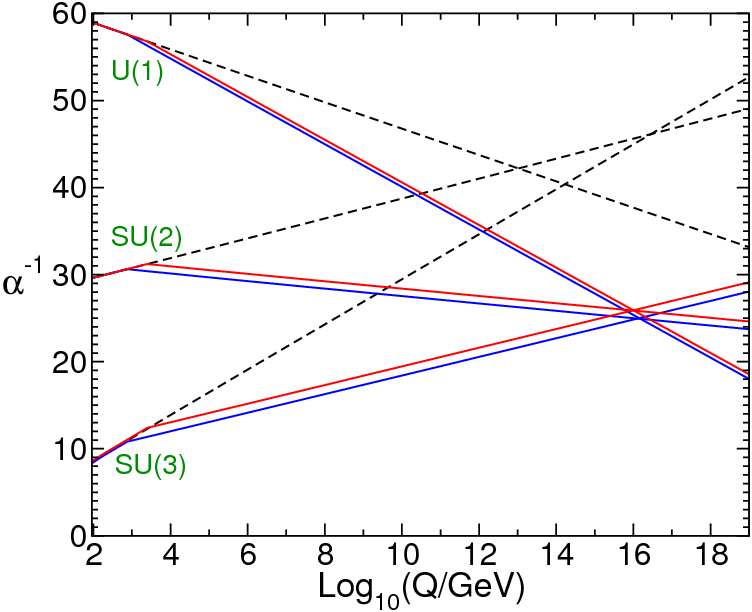
\includegraphics[width=\textwidth]{images/gauge_coupling_unification}
    \legend{The sparticle masses are varied between 0.5-1.5 TeV, and $\alpha_3(m_Z)$ is varied between 0.117 and 0.121.}
  \label{fig:gauge_coupling_unification}
\end{marginfigure}
\noindent The minimal phenomenologically viable incorporation of supersymmetry into the Standard Model is known as the \emph{Minimal Supersymmetric Standard Model}, or the MSSM. Although the hierarchy problem has been the main driving force behind the development of supersymmetry, there are other motivations to study it as well.
One of them is that it has the right particle content to unify the strong and electroweak couplings at a high energy scale, as seen in \autoref{fig:gauge_coupling_unification}.

The third major motivation (and the one most relevant to this dissertation) is the fact that the MSSM contains a viable dark matter candidate. The theory admits a new kind of discrete symmetry known as \emph{R-parity}, which is an analogue of baryon and lepton number conservation. The Lagrangian of the MSSM is defined to be invariant under the action of the operator $P_R$, with eigenvalues $(-1)^{3(B-L)+2s}$, where \emph{B, L}, and \emph{s} represent the baryon number, lepton number, and spin of the field that is acted upon, respectively. As a consequence of this symmetry, the lightest supersymmetric particle (LSP) cannot decay further into other particles, thus making it a good candidate for dark matter.

\subsection{The supersymmetry algebra}
In 1967, Coleman and Mandula \citep{Coleman:1967ad} showed that, given certain assumptions, the only possible Lie group symmetries allowed for relativistic interacting field theories in four dimensions are direct products of the Poincar\'e group and an internal symmetry group (i.e. a gauge symmetry) \citep{Mandula:2015}.
A Lie algebra is defined by the commutation relations of its generators. If we extend the notion of a Lie algebra to include \emph{anticommutation} relations \citep{Wess:1974tw}, this restriction no longer applies. These kinds of algebras are known as \emph{graded Lie algebras}, or \emph{superalgebras}. The trio of Haag, Łopuszanski, and Sohnius \citep{Haag:1974qh} applied a similar treatment as Coleman and Mandula to determine the most general superalgebra consistent with relativistic quantum field theory. The generators $Q_\alpha$ of this algebra are known as fermionic operators, and must transform as Weyl spinors. The anticommutation (and commutation) relations take the form
\sidepar{The supersymmetry algebra}
\begin{align}
  \begin{split}
  \{Q_\alpha, \bar{Q}_{\dot{\beta}}\} &= 2(\sigma^\mu)_{\alpha\dot{\beta}}P^\mu\\
  \{Q_\alpha, Q_\beta\} &= \{\bar{Q}_{\dot{\alpha}}, \bar{Q}_{\dot{\beta}}\} = 0\\
  [P^\mu,Q_\alpha] &= [P^\mu,\bar{Q}_{\dot{\alpha}}] = 0
\end{split}
\label{eq:susy_algebra}
\end{align}
where $P_\mu = i\partial_\mu$ is the generator of translations. 

The first supersymmetric Lagrangian density in four-dimensions was formulated by Wess and Zumino \citep{Wess:1974tw}. The approach taken was to define infinitesimal `supergauge' transformations for scalars and spinors that generated a closed algebraic structure. Soon afterwards, Salam and Strathdee \citep{Salam:1974yz} created a more systematic approach to constructing these transformations, by giving them a geometric interpretation. 

In this picture, supersymmetric transformations can be viewed as translations in a manifold known as \emph{superspace}, which is obtained by adding the `fermionic' coordinates $\theta^\alpha$ and $\bar{\theta}^{\dot{\beta}}$ to the regular `bosonic' spacetime coordinates $x^\mu$. 
\sidepar{Generators of superspace translations}
The generators of these translations are represented by
\begin{align}
  Q_\alpha &= \frac{\partial}{\partial\theta^\alpha}-i(\sigma^\mu \bar{\theta})_\alpha \partial_\mu&&\text{and}&&
  \bar{Q}_{\dot{\beta}} = \frac{\partial}{\partial\bar{\theta}^{\dot{\beta}}}-i(\sigma^\mu\bar{\theta})_{\dot{\beta}}\partial_\mu.
\label{eq:susy_operators_diff_form}
\end{align}
These transformations act on objects known as superfields, which are complex scalar fields parameterized by the coordinates $(x^\mu,\theta,\bar{\theta})$.
Under an infinitesimal supersymmetry transformation, a general superfield $S(x,\theta,\bar{\theta})$ transforms as
\begin{align}
S\rightarrow S' = (1+i\xi^\alpha Q_\alpha + i\bar{\xi}_{\dot{\alpha}}\bar{Q}^{\dot{\alpha}})S
\label{eq:gen_susy_transformation}
\end{align}
where $\xi^\alpha$ and $\bar{\xi}_{\dot{\alpha}}$ are two-component Weyl spinor fields that parameterize the translation.
The fermionic coordinates $\theta$ and $\bar{\theta}$ each have two components. For example, $\theta$ can be represented as $\theta^\alpha = (\theta^1,\theta^2)$. Each of these two components is a \emph{Grassmannian} variable, satisfying the anticommutation relation $\{\theta^i,\theta^i\} = 0$. This implies that $(\theta^i)^2 = 0$. This means that a Taylor expansion in powers of a fermionic coordinate must always terminate with a finite number of terms. For a general superfield \emph{S}, the Taylor expansion about the fermionic coordinates $\theta,\bar{\theta}$ takes the form
\sidepar{General superfield expansion}
\begin{align}
  \begin{split}
  S(x,\theta,\bar{\theta}) = a &+ \theta\xi + \bar{\theta}\chi^\dagger + \theta\theta b + \bar{\theta}\bar{\theta}c+\bar{\theta}\bar{\sigma}^\mu\theta v_\mu \\
  &+ \bar{\theta}\bar{\theta}\theta\eta + \theta\theta\bar{\theta}\zeta^\dagger+\theta\theta\bar{\theta}\bar{\theta}d,
\end{split}
  \label{eq:general_superfield_expansion}
\end{align}
where \emph{a,b,c} and \emph{d} are complex-valued scalar fields, $\xi,\chi,\eta$ and $\zeta$ are spinor fields, and $v_\mu$ is a vector field. These coefficients in the Taylor expansion will be identified with the regular (non-super) fields that we see in the SM and its supersymmetrized version, the MSSM. The matter content of the MSSM can be derived from expanding superfields of a particular type, known as \emph{chiral} superfields, with mass dimension 1. The expansion of a generic chiral superfield $\Phi$ takes the form:
\sidepar{Chiral superfield expansion}
\begin{align}
  \begin{split}
  \Phi(y,\theta) &= \phi(x) + \sqrt{2}\theta\psi(x)+\theta\theta F(x)\\
  &+i\theta\sigma\bar{\theta}\partial_\mu\phi(x)-\frac{1}{2}\theta\sigma\bar{\theta}\theta\sigma^\nu\bar{\theta}\partial_\mu\partial_\nu\phi(x) + \sqrt{2}\theta i\theta\sigma\bar{\theta}\partial_\mu\psi(x)
\end{split}
  \label{eq:chiral_superfield_expansion}
\end{align}
Similarly the gauge bosons come from the expansion of dimension-0 \emph{vector} superfields $V$, obtained by imposing the condition $V = V^\dagger$. 
\sidepar{Vector superfield expansion}
The expansion of $V$ takes the form:
\begin{align}
V = \bar{\theta}\bar{\sigma}^\mu\theta A_\mu+\bar{\theta}\bar{\theta}\theta\lambda+\theta\theta\bar{\theta}\lambda^\dagger+\frac{1}{2}\theta\theta\bar{\theta}\bar{\theta}D.
\label{eq:vector_superfield_expansion}
\end{align}
We see that the expansion of the chiral superfield $\Phi$ contains a scalar field $\phi$, a Weyl fermion $\psi$, and a field $F$. Thus, choosing values of $\phi,\psi$, and $F$ fixes $\Phi$. These fields, known as the \emph{component fields} of $\Phi$ can be naturally placed in a collection known as a \emph{supermultiplet}. The scalar superpartners $\phi$ are referred to as \emph{sfermions}. 
Similarly, the vector field $A_\mu$, the fermion field $\lambda$, and the field \emph{D} form another natural grouping, called a \emph{vector} supermultiplet. The fields $A_\mu$ and $\lambda$ are superpartners of each other, and fields such as $\lambda$ are generically known as \emph{gauginos}. The particle content of the MSSM, grouped into supermultiplets, is shown in tables \ref{tab:chiral_supermultiplets} and \ref{tab:gauge_supermultiplets}. For brevity, we have not shown all three fermion generations. Also, the fields $F$ and $D$ are not included, since they are \emph{auxiliary} fields, serving only to make sure that supersymmetry holds off-shell. The gauge structure of the MSSM is the same as that of the SM - there are no new gauge interactions.

The mass terms and Yukawa terms of the MSSM Lagrangian come from the collection of terms known as the \emph{superpotential}. 
\sidepar{The MSSM superpotential}
In terms of the chiral superfields in \autoref{tab:chiral_supermultiplets}, we can write the MSSM superpotential as:
\[W_\text{MSSM} = \overline{u}\mathbf{y_u}QH_u-\overline{d}\mathbf{y_d}Q H_d-\overline{e}\mathbf{y_e}L H_d+\mu H_u H_d \]
Here, we have abbreviated terms such as $\mu(H_u)_\alpha (H_d)_\beta\epsilon^{\alpha\beta}$ to $\mu H_u H_d$. The matrices $\mathbf{y}$ are $3\times3$ matrices of Yukawa couplings, with indices corresponding to the three generations of fermions. Note also that we now see the necessity of having two Higgs doublets - one that couples to the up-type fermions, and the other to the down-type fermions. A term like $\overline{u}\mathbf{y_u}QH_d^*$ would lead to a non-conserved hypercharge.

\subsection{Softly broken supersymmetry}
The component fields of a superfield have the same mass, as can be seen from expansions of the chiral and vector superfields in \eqref{eq:chiral_superfield_expansion} and \eqref{eq:vector_superfield_expansion}. This means that if supersymmetry holds, the superpartners of the SM particles should have been discovered by now. Evidently, if this symmetry exists, it is not apparent in the ground state that we inhabit - that is, it must be spontaneously broken. The exact mechanism by which it is broken is still unknown - there are a number of competing models which introduce new physics at high energy scales to spontaneously break supersymmetry. To remain model-agnostic, we can parameterize our ignorance by inserting the relevant terms into the Lagrangian by hand, with their form constrained by the requirement that the quadratic divergences in the radiative corrections to scalar masses must still vanish.

\begin{table}
  \caption{Chiral supermultiplets of the MSSM.}
  \begin{tabular}{cccccc}
    \toprule
                    & \multicolumn{2}{c}{Components}                  & \multicolumn{3}{c}{Group representation} \\ \cmidrule(r){2-3}\cmidrule(l){4-6}
    Superfield      & Spin-0                                          & Spin-$\slantfrac{1}{2}$                                                        & $SU(3)$            & $SU(2)$      & $U(1)_Y$\\\midrule
                    & Squarks                                         & Quarks                                                                         &                    &              & \\ \cmidrule(r){2-3}\\
    Q               & $\vdoublet{\widetilde{u}_L}{\widetilde{d}_L}$   & $\vdoublet{u_L}{d_L}$                                                          & $\mathbf{3}$       & $\mathbf{2}$ & $\frac{1}{2}$\\\\
    $\overline{u}$  & $\tilde{u}_R^*$                                 & $u_R^\dagger$                                                                  & $\bar{\mathbf{3}}$ & $\mathbf{1}$ & -$\frac{2}{3}$\\\\
    $\overline{d}$  & $\tilde{d}_R^*$                                 & $d_R^\dagger$                                                                  & $\bar{\mathbf{3}}$ & $\mathbf{1}$ & $\frac{1}{3}$\\\\\cmidrule{2-3}
                    & Sleptons                                        & Leptons                                                                        &                    &              & \\ \cmidrule{2-3}\\
    \emph{L}        & $\vdoublet{\widetilde{\nu}_L}{\widetilde{e}_L}$ & $\vdoublet{\nu_L}{e_L}$                                                        & $\mathbf{1}$       & $\mathbf{2}$ & -$\frac{1}{2}$\\\\
    $\overline{e}$  & $\tilde{e}_R^*$                                 & $e_R^\dagger$                                                                  & $\bar{\mathbf{1}}$ & $\mathbf{1}$ & $1$\\\\\cmidrule{2-3}
                    & Higgses                                         & Higgsinos                                                                      &                    &              & \\ \cmidrule{2-3}\\
    $H_u$           & $\vdoublet{H_u^+}{H_u^0}$                       & $\vdoublet{\widetilde{H}_u^+}{\widetilde{H}_u^0}$                              & $\mathbf{1}$       & $\mathbf{2}$ & $\frac{1}{2}$\\\\
    $H_d$           & $\vdoublet{H_d^0}{H_d^-}$                       & $\vdoublet{\widetilde{H}_d^0}{\widetilde{H}_d^-}$                              & $\mathbf{1}$       & $\mathbf{2}$ & -$\frac{1}{2}$\\\\
    \bottomrule
  \end{tabular}
  \label{tab:chiral_supermultiplets}
\end{table}

\begin{table}
  \caption{Gauge supermultiplets of the MSSM.}
  \begin{tabular}{ccccc}
    \toprule
\multicolumn{2}{c}{Components} & \multicolumn{3}{c}{Group representation} \\ \cmidrule(r){1-2}\cmidrule(l){3-5}
Spin-$\slantfrac{1}{2}$        & Spin-1                                                                         & $SU(3)$          & $SU(2)$    & $U(1)_Y$\\\midrule
Gluinos: $\widetilde{g}$       & Gluons: \emph{g}                                                               & $\mathbf{8}$       & $\mathbf{1}$ & $0$ \\\\
Winos: $\widetilde{W}^0$       & \emph{W} bosons: $W^\pm$                                                              & $\bar{\mathbf{1}}$ & $\mathbf{3}$ & $0$\\\\
Binos: $\widetilde{B}^0$       & \emph{B} bosons: $B^0$                                                                & $\bar{\mathbf{1}}$ & $\mathbf{3}$ & $0$\\
    \bottomrule
  \end{tabular}
  \label{tab:gauge_supermultiplets}
\end{table}

The soft supersymmetry breaking terms of the MSSM, written in terms of the component fields from tables \ref{tab:chiral_supermultiplets} and \ref{tab:gauge_supermultiplets} are as follows.
\sidepar{Soft supersymmetry breaking terms}
\begin{align*}
  \begin{split}
    \mathcal{L}_\text{soft}^\text{MSSM} = &-\frac{1}{2}\left(M_1\widetilde{B}\widetilde{B}+
    M_2\widetilde{W}\widetilde{W} + M_3\widetilde{g}\widetilde{g} + \text{h.c.}\right)\\
    &-\left(\widetilde{\overline{u}}\mathbf{a_u}\widetilde{Q}H_u-
    \widetilde{\overline{d}}\mathbf{a_d}\widetilde{Q}H_d-
    \widetilde{\overline{e}}\mathbf{a_e}\widetilde{L}H_d+\text{h.c.}\right)\\
    &-\widetilde{Q}^\dagger\mathbf{m}_{\widetilde{Q}}^2\widetilde{Q}
     -\widetilde{L}^\dagger\mathbf{m}_{\widetilde{L}}^2\widetilde{L}
     -\widetilde{\overline{u}}^\dagger\mathbf{m}_{\widetilde{\overline{u}}}^2\widetilde{\overline{u}}^\dagger
     -\widetilde{\overline{d}}^\dagger\mathbf{m}_{\widetilde{\overline{d}}}^2\widetilde{\overline{d}}^\dagger
     -\widetilde{\overline{e}}^\dagger\mathbf{m}_{\widetilde{\overline{e}}}^2\widetilde{\overline{e}}^\dagger\\
     &-m^2_{H_u}H^*_uH_u-m^2_{H_d}H_d^*H_d-(bH_uH_d+\text{h.c.}) 
  \end{split}
  \label{eq:soft_susy_breaking_terms}
\end{align*}
The tildes denote superpartners of the corresponding SM fields. The parameters $M_1$, $M_2$, $M_3$ govern the masses of the gauginos $\widetilde{B}$, $\widetilde{W}$, and $\widetilde{g}$, respectively.

\subsection{Phenomenological approximations}
The MSSM has a number of simplifying assumptions motivated both by calculational convenience and compatibility with observed experimental data. For example, it is convenient to take the Yukawa matrices $\mathbf{y_u,y_d,y_e}$ in a simplified limit, where only the heaviest generations have non-zero Yukawa couplings:
\begin{align*}
  \mathbf{y_u} \approx \begin{pmatrix}
    0 & 0 & 0\\
    0 & 0 & 0\\
    0 & 0 & y_t
  \end{pmatrix},&&
  \mathbf{y_d} \approx \begin{pmatrix}
    0 & 0 & 0\\
    0 & 0 & 0\\
    0 & 0 & y_b
  \end{pmatrix},&&
  \mathbf{y_e} \approx \begin{pmatrix}
    0 & 0 & 0\\
    0 & 0 & 0\\
    0 & 0 & y_\tau
  \end{pmatrix}.
\end{align*}
Furthermore, to suppress excessive CP-violation and flavor-changing neutral currents in the MSSM, the following approximations are often made. First, we assume that there is minimal mixing among the sfermions:
\begin{align*}
  \mathbf{m}_{\widetilde{Q}}^2 = m_{\widetilde{Q}}^2\mathbf{1},&&
  \mathbf{m}_{\widetilde{\overline{u}}}^2 = m_{\widetilde{\overline{u}}}^2\mathbf{1},&&
  \mathbf{m}_{\widetilde{\overline{d}}}^2 = m_{\widetilde{\overline{d}}}^2\mathbf{1},&&
  \mathbf{m}_{\widetilde{\overline{e}}}^2 = m_{\widetilde{\overline{e}}}^2\mathbf{1},&&
  \mathbf{m}_{\widetilde{L}}^2 = m_{\widetilde{L}}^2\mathbf{1}\\
\end{align*}
We also suppress the cubic scalar couplings of the first two families of sfermions by imposing the conditions: 
\begin{align*}
  \mathbf{a_u} = A_{u0}\mathbf{y_u},&&
  \mathbf{a_d} = A_{d0}\mathbf{y_d},&&
  \mathbf{a_e} = A_{e0}\mathbf{y_e}.\\
\end{align*}
Finally, requiring that the soft SUSY breaking parameters are real enables us to suppress excessive amounts of CP violation:
\begin{align*}
  \text{Im}(M_1)=
  \text{Im}(M_2)=
  \text{Im}(M_3)=
  \text{Im}(A_{u0})=
  \text{Im}(A_{d0})=
  \text{Im}(A_{e0})=0.
\end{align*}
With the above ingredients, one can work out myriad phenomenological consequences. In \autoref{ch:DM_100_TeV}, we examine the neutralino sector of the MSSM in slightly more detail, and present an analysis aimed at exploring it at a 100 TeV collider.

%\chapter{Two-Higgs Doublet Models}\label{ch:2HDMs}

Intuitively, it is not too hard to imagine, based on the complex structure of the fermion and gauge sectors, that the scalar sector of the Standard Model might well contain members other than a single $SU(2)$ doublet. The possible extensions to the scalar sector are constrained by the value of the parameter $\rho$. For a $SU(2)\times U(1)$ gauge theory, this takes the form (at tree level):

\begin{equation}
\rho = \frac{\sum_\text{i=1}^n\left[I_i(I_i+1)-\frac{1}{4}Y_i^2Y_i^2\right]v_i}{\sum_\text{i=1}^n\frac{1}{2}Y_i^2v_i}
\end{equation}
%
where $n$ is the number of scalar multiplets with isospin\footnote{Short for \emph{isotopic spin}} $I_i$, hypercharge $Y_i$, and vacuum expectation values of the neutral components $v_i$. This parameter has been experimentally measured to be almost exactly one. The simplest extensions to the scalar sector that satisfy this constraint involve adding additional scalar singlets and doublets. The ones that add a single additional $SU(2)$ scalar doublet field are collectively known as \emph{Two-Higgs Doublet Models}, or 2HDMs. For a detailed review of 2HDMs, see \citep{Branco2012}, whose treatment we follow closely here.

Adding an additional scalar doublet alleviates some of the problems with the Standard Model that we mentioned at the end of the previous chapter. 
% Strong CP problem
Lagrangians for Yang-Mills theories can have a renormalizable term that is gauge-invariant but but violates CP, of the form
\[\mathcal{L}_{\theta} = \theta\epsilon^{\mu\nu\alpha\beta}F_{\mu\nu}^aF_{\alpha\beta}^a\]
where $\theta$ is some angle, $F_{\mu\nu}$ is the field strength tensor, and $\epsilon^{\mu\nu\alpha\beta}$ is an antisymmetric tensor\footnote{Levi-Civita?}. This term is a total derivative, since it can be written as $2\theta\partial_\mu(\epsilon^{\mu\nu\alpha\beta}A_\nu^aF_{\alpha\beta}^a)$. Thus, it should not contribute to perturbative effects. However, this term can potentially contribute to non-perturbative effects. Additionally, this term can be modified by chiral rotations of the form $\psi\rightarrow \exp(i\gamma_5\theta_F)\psi$. Since physical observables should be independent of the choice of the basis, i.e. $\theta_F$, we should absorb it into $\theta$ by defining a basis-independent phase: $\bar{\theta} = \theta-\theta_F$. For $SU(2)$ and $U(1)$ gauge symmetries, this phase can be set to zero by performing appropriate chiral rotations of the fermion fields. However, no such choice exists for the term corresponding to the the $SU(3)$ group, and thus the CP-violating term in the QCD Lagrangian could in principle by non-zero. A non-zero value of $\bar{\theta}$ would be manifested as non-perturbative effects. For example, the neutron would then have a non-zero electric dipole moment. However, experiments have shown that $\bar{\theta}$ must be vanishingly small, with a stringent upper bound: $\bar{\theta}<10^{-10}$.

Adding an additional scalar doublet allows us to impose a global $U(1)$ symmetry on the Lagrangian, known as \emph{Peccei-Quinn} symmetry. If this symmetry is spontaneously broken, a Goldstone boson arises, which can then be chirally rotated such that $\bar{\theta}$ becomes effectively zero for the ground state.
% Baryon asymmetry
Another motivation for 2HDMs is their ability to explain the observed baryon asymmetry of the universe. That is, the amount of matter in the universe is much larger than the amount of antimatter in it. The CP violation in the weak sector the Standard Model cannot account for this imbalance, but 2HDMs, with their complex scalar sector and possible new sources of CP violation, can.
%
The strongest motivation for 2HDMs is, however, the potential to resolve the hierarchy problem. More specifically, supersymmetric theories provide a way to resolve the hierarchy problem, as discussed in \autoref{ch:supersymmetry}. These theories require an additional scalar doublet to give mass to both up- and down-type fermions, and for the cancellation of anomalies.

\section{The 2HDM Lagrangian}
The most general renormalizable scalar potential for two doublets $\Phi_1$ and $\Phi_2$ with hypercharge $+1$ is:

\begin{align*}
  V(\Phi_1,\Phi_2) &= m_{11}^2|\Phi_1|^2 + m_{22}^2|\Phi_2|^2 - m_{12}^2\left(\Phi_1^\dagger\Phi_2 + h.c.\right)\\
&+\frac{\lambda_1}{2}|\Phi_1|^4 + \frac{\lambda_2}{2}|\Phi_2|^4+\lambda_3|\Phi_1|^2|\Phi_2|^2 + \lambda_4|\Phi_1^\dagger\Phi_2|^2\\
&+\frac{\lambda_5}{2}\left[\left(\Phi_1^\dagger\Phi_2 \right)^2+\lambda_6|\Phi_1|^2(\Phi_1^\dagger\Phi_2)+\lambda_7|\Phi_2|^2(\Phi_1^\dagger\Phi_2) + h.c.\right]
\label{eq:2HDM_scalar_potential}
\end{align*}
where $h.c.$ stands for the hermitian conjugate. The parameters $m_{11}, m_{22}$, and $\lambda_{1,2,3,4}$ are real while $m_{12}$ and $\lambda_{5,6,7}$ can be complex. Naively, it would seem that this potential has 14 degrees of freedom - six from the real parameters, and eight from the complex parameters. However, it should be noted that we have the freedom to perform basis transformations, that is, we can write the potential in terms of new doublets $\Phi_a' = \sum_{b=1}^2U_{ab}\Phi_b$. where $U_{ab}$ is a $2\times 2$ unitary matrix. The condition of unitarity implies that $U$ has three degrees of freedom, which can absorb three out of the 14 degrees of freedom listed earlier. Thus, only 11 out of the original 14 degrees of freedom are physical.

In principle, we could proceed with these 11 parameters, however, there are a couple of reasons to attempt to reduce this number. The first is that a large number of free parameters makes a theory less falsifiable, thus reducing its predictive power. The second is that in order to distinguish between pseudoscalars and scalars, CP must be conserved in the Higgs sector. Finally, the potential in \eqref{eq:2HDM_scalar_potential} allows for tree-level flavor-changing neutral currents (FCNC), which are experimentally measured to be highly suppressed. These can be eliminated by introducing discrete or continuous symmetries. Imposing a discrete symmetry such as $\mathcal{Z}_2$, that is, the Lagrangian is invariant under the reflection of one of the doublets: $\Phi_i\rightarrow-\Phi_i$, removes the terms that are odd in $\Phi_i$. This effectively sets $\lambda_6=\lambda_7 = 0$. In principle, this should set $m_{12} = 0$ as well, but we retain this term since it breaks the $\mathcal{Z}_2$ symmetry softly, which relaxes the experimental bounds on the mass spectrum.
After imposing these constraints, all the remaining parameters $\lambda_{1,2,3,4,5}, m_{11,12,22}$ are real. From here on, we will only consider 2HDMs with these constraints. 

There are four such models, classified based on the coupling patterns of the fermions to the two Higgs doublets. In type-I 2HDMs, all the quarks couple to only one of the Higgs doublets (chosen by convention to be $\Phi_2$. In type-II 2HDMs, the up-type right-handed quarks (\emph{u,c,t}) couple to $\Phi_2$, and the down-type right-handed quarks (\emph{d,s,b}) couple to $\Phi_1$. In both of these models, the right-handed leptons couple to the same doublet as the down-type quarks. There are two other models that do not have tree-level FCNCs. The lepton-specific model is similar to the type-I model, except in this case, the right-handed leptons couple to $\Phi_1$. Similarly, the `flipped' model is similar to the type-II 2HDM, except that the leptons couple to $\Phi_2$. The coupling patterns for these models are collected in \autoref{tab:no_FCNC_2HDMs}.

\begin{margintable}
\small{
  \begin{tabular}{lccc}
	\toprule
    Model & $u_R^i$ & $d_R^i$  & $e_R^i$\\
    \midrule
    Type I          & $\Phi_2$ & $\Phi_2$ & $\Phi_2$\\
    Type II         & $\Phi_2$ & $\Phi_1$ & $\Phi_1$\\
    Lepton-specific & $\Phi_2$ & $\Phi_2$ & $\Phi_1$\\
    Flipped         & $\Phi_2$ & $\Phi_1$ & $\Phi_2$\\
    \bottomrule
  \end{tabular}}
  \caption{2HDMs with flavor conservation.}
  \label{tab:no_FCNC_2HDMs}
\end{margintable}

This potential is minimized for non-zero vacuum expectation values of $\Phi_i$:
\begin{align}
\langle\Phi_i\rangle_0=\vdoublet{0}{\frac{v_i}{\sqrt{2}}}
\end{align}
The complex scalar $SU(2)$ doublets $\Phi_i$ can be expressed in terms of eight real fields as follows:
\begin{equation}\label{eq:2HDM_doublet_components}
\Phi_i = \vdoublet{\phi_i^+}{\frac{1}{\sqrt{2}}(v_i+\rho_i+i\eta_i)}
\end{equation}
The process of electroweak symmetry breaking causes three of these fields to be `eaten' by the \emph{W} and \emph{Z} bosons, and the remaining five are manifested as physical scalar fields. These consist of a pair of CP-even neutral scalars \emph{h} and \emph{H}, a CP-odd pseudoscalar \emph{A}, and a charged scalar $H^\pm$.

\section{The 2HDM mass spectrum}

In this section, we will analyze the mass spectrum of flavor-conserving 2HDMs. To do so, we construct the mass matrices by taking derivatives of the scalar potential:
\[M_{ij} = \frac{\partial V(\Phi_1,\Phi_2)}{\partial\phi_i\partial\phi_j}\]
where $\phi_{i}$ can be any of the fields $\phi_i^+,\rho_i,\eta_i$ in \eqref{eq:2HDM_doublet_components}. We will also adopt the notation: 
Applying this procedure to the charged scalar components $\phi_i^\pm$, we obtain their mass matrix $M_{\phi^{\pm}}$:
\[M_{\phi^\pm} = \left[m_{12}^2-(\lambda_4+\lambda_5)v_1v_2\right]\fourmatrix{v_2/v_1}{-1}{-1}{v_1/v_2}\]
Diagonalizing this matrix gives us the mass of the charged Higgses:
\[m_{H^\pm}^2 = (v_1^2+v_2^2)[m_{12}^2/v_1v_2-(\lambda_4+\lambda_5)]\]
Similarly, the mass matrix for the pseudoscalars is given by
\[M_{\eta} = \frac{m_A^2}{v_1^2+v_2^2}\fourmatrix{v_2^2}{-v_1v_2}{-v_1v_2}{v_1^2}\]
Diagonalizing this matrix gives us a massless Goldstone boson $G^0$, corresponding to a zero eigenvalue, and a pseudoscalar Higgs boson $A$, with mass given by:
\[m_A^2 = (v_1^2+v_2^2)[m_{12}^2/v_1v_2-2\lambda_5]\]
The diagonalization process amounts to a rotation of the basis vectors by some angle.For the CP-odd and the charged scalars, this angle is the same, and is denoted as $\beta$. Let us now adopt the notation 
\[s_\theta,c_\theta,t_\theta = \sin\theta,\cos\theta,\tan\theta\]
for conciseness. In this notation, the mass eigenstates are given by
\begin{align}
\vdoublet{A}{G^0} = \fourmatrix{s_\beta}{-c_\beta}{c_\beta}{s_\beta}\vdoublet{\eta_1}{\eta_2}&&\text{and}&&
\vdoublet{H^\pm}{G^\pm} = \fourmatrix{s_\beta}{-c_\beta}{c_\beta}{s_\beta}\vdoublet{\phi_1^+}{\phi_2^+}.
\end{align}
The angle $\beta$ turns out to be a very important one for studying 2HDMs. It also represents the ratio of the vacuum expectation values of the neutral components of the two Higgs doublets: $t_\beta = v_2/v_1$.
Finally, the mass matrix for the CP-even scalars is given by:
\[M_{\rho} = -\fourmatrix{m_{12}^2\frac{v_2}{v_1}+\lambda_1v_1^2}{-m_{12}^2+\lambda_{345}v_1v_2}{-m_{12}^2+\lambda_{345}v_1v_2}{m_{12}^2\frac{v_2}{v_1}+\lambda_1v_2^2}\]
where $\lambda_{345} = \lambda_3+\lambda_4+\lambda_5$. This matrix is diagonalized by rotation of the basis vectors by the angle $\alpha$:
\[\vdoublet{h}{H} = \fourmatrix{s_\alpha}{-c_\alpha}{-c_\alpha}{-s_\alpha}\vdoublet{\rho_1}{\rho_2}\]
with the mass eigenstates denoted $h,H$. Traditionally, $h$ is taken to be the ligher of the two particles. 

%\begin{align}
%v &= v_1^2 + v_2^2
%\end{align}
Thus we see that the physical spectrum of 2HDMs contains five mass eigenstates: the CP-even higgses $h$ and $H$, the CP-odd pseudoscalar Higgs $A$, and a pair of charged Higgses $H^\pm$. Incidentally, the standard model Higgs is a combination of the CP-even scalars:
\begin{equation}
h_\text{SM} = \rho_1\cos\beta + \rho_2\sin\beta = h\sin(\alpha-\beta)-H\cos(\alpha-\beta)
\label{eq:h_SM}
\end{equation}


\section{Interactions}

\newcommand{\sbma}{s_{\beta-\alpha}}
\newcommand{\cbma}{c_{\beta-\alpha}}
\newcommand{\casb}{c_\alpha/s_\beta}
\newcommand{\sacb}{s_\alpha/c_\beta}
\newcommand{\sasb}{s_\alpha/s_\beta}
\begin{table}
  \[
    \begin{array}{lrrrr}
      \toprule
         & \text{Type I} & \text{Type II} & \text{Lepton-specific} & \text{Flipped}\\
         \midrule
      \xi_{hVV} & \sbma & \sbma & \sbma & \sbma \\
      \xi_{h}^u & \casb & \casb & \casb & \casb \\
      \xi_{h}^d & \casb & -\sacb & \casb & -\sasb \\
      \xi_{h}^l & \casb & -\sacb & -\sasb & -\casb \\
      \xi_{HVV} & \cbma & \cbma  & \cbma & \cbma \\
      \xi_{H}^u & \sasb & \sasb & \sasb & \sasb \\
      \xi_{H}^d & \sasb & \casb & \sasb & \casb \\
      \xi_{H}^l & \sasb & \casb & \casb & \sasb \\
      \xi_{AVV} & 0     & 0     & 0     & 0 \\
      \xi_{A}^u & 1/t_\beta & 1/t_\beta & 1/t_\beta & 1/t_\beta \\
      \xi_{A}^d & -1/t_\beta & t_\beta & -1/t_\beta & t_\beta \\
      \xi_{A}^l & -1/t_\beta & t_\beta & t_\beta & -1/t_\beta \\
      \bottomrule
\end{array}\]
\caption{List of the factors $\xi$ that determine the Yukawa couplings of the 2HDM Higgs bosons.}
\label{tab:xi_factors}
\end{table}

We will first consider the Yukawa interactions of the mass eigenstates with fermions, which are given by:
\begin{align*}
\mathcal{L}^{\mathrm{2HDM}}_{\text{Yukawa}} =& - \sum_{f = u, d, l} \frac{m_f}{v}
\left(\xi_h^f \overline{f}fh+\xi_H^f \overline{f}fH-i\xi_A^f \overline{f}\gamma_5fA \right)\\
&-\left\{\frac{\sqrt{2}V_{ud}}{v}\overline{u}\left(m_u\xi_A^uP_l+m_d\xi_A^dP_R\right)dH^+ + \frac{\sqrt{2}m_l\xi^l_A}{v}\overline{\nu}_Ll_RH^+ + h.c.\right\}
\end{align*}
where $f$ is a fermion with mass $m_f$, $u,d$ refer to up- and down-type quarks with masses $m_u,m_d$ and CKM mixing $V_{ud}$, $l$ is a lepton with mass $m_l$, and $\nu_L$ is a neutrino. 
As for the Yukawa couplings to the vector bosons, we can recover them by recalling that the standard model Higgs is given by
\begin{equation}
h_\text{SM} = hs_{\alpha-\beta}-Hc_{\alpha-\beta}.
\end{equation}
Thus the couplings of \emph{h} and \emph{H} become rescaled versions of standard model Higgs couplings to the vector bosons. If we represent these couplings by $g_{h_\text{SM}VV}$, where $VV$ can be $ZZ$ or $W^+W^-$, then the Yukawa couplings of the 2HDM Higgses are given by
\begin{align}
g_{\phi VV} = \xi_{\phi VV}g_{h_\text{SM}VV},
\end{align}
where $\phi = h/H/A$. The factors $\xi$ in the above expressions depend on the specific model being considered, and are listed in \autoref{tab:xi_factors}.

With a little bit of work (we omit the details for brevity), we can extract the following couplings\footnote{\Adarsh{I need to double check the signs of these couplings.}} (see \citep{Kling2016a} for details):
\begin{align*}
g_{\gamma H^+H^-} &= -ie(p_{H^+}-p_{H^-})^\mu\\
g_{ZH^+H^-} &= -i\frac{gc_{2\theta_w}}{2c_{\theta_w}}(p_{H^+}-p_{H^-})^\mu\\
g_{AH^\pm W^\mp} &= \frac{g}{2}(p_{H^+}-p_{A})^\mu\\
g_{hAZ} &= is_{\beta-\alpha}\frac{g}{2c_{\theta_w}}(p_A-p_h)^\mu\\
g_{hH^\pm W^\mp} &= -is_{\beta-\alpha}\frac{g}{2}(p_{H^\pm}-p_h)^\mu\\
g_{HAZ} &= ic_{\beta-\alpha}\frac{g}{2c_{\theta_w}}(p_A-p_H)^\mu\\
g_{HH^\pm W^\mp} &= -ic_{\beta-\alpha}\frac{g}{2}(p_{H^\pm}-p_H)^\mu\\
\end{align*}

The cubic and quartic Higgs couplings can also be worked out explicitly, but we will decline to do so and instead refer the reader to the general expressions in Appendix C of  \citep{Branco2012} and the specific expressions in section 2.3.3 of \citep{Kling2016a}. 

\section{The Type-II 2HDM}

As mentioned at the beginning of this chapter, The type-II 2HDM is of special interest since it has the same fermion-Higgs doublet coupling pattern as the MSSM. In fact, the MSSM can be viewed as a special case of a type-II 2HDM, one that incorporates supersymmetry. We will examine the MSSM in more detail in the next section, but will note that if we can recover the tree-level MSSM scalar potential from a type-II 2HDM by setting the parameters $\lambda_i$ to the following values:
\begin{align}
\lambda_{1,2} = \frac{g^2+g'^2}{2} &,& \lambda_3 = \frac{g^2-g'^2}{4} &,& \lambda_4 = -\frac{g^2}{2}&,&\lambda_{5,6,7} = 0.
\end{align}
It should be noted, however, that these relations do not hold beyond the tree-level for a generic non-supersymmetrized 2HDM.
The analyses in (section about light charged Higgs) and (section about Exotic Higgs at 100 TeV) are designed to probe the parameter space of a type-II Two Higgs Doublet Model.

%\chapter{Supersymmetry and the MSSM}\label{ch:supersymmetry}

Historically, examining nature at increasing energy scales (and correspondingly decreasing length scales ) has consistently yielded new physics. For example, higher-energy experiments were able to probe the structure of the weak interactions, precisely at the energy scale that the 4-Fermi theory started to fail. Similarly, the challenges listed at the end of \autoref{ch:sm} most likely point to new physics at higher energy scales, between the currently explored weak scale to the reduced Planck scale:
\begin{equation*}
M_P = 1/\sqrt{8\pi G} \approx 2.4\times 10^{18} \text{ GeV}
\end{equation*}
However, the SM Higgs potential is extremely sensitive to new physics at high energies. The mass of the SM Higgs boson receives large quantum corrections from any new physics at high energies that couples to the Higgs sector. For example, if the Higgs couples to a heavy fermion \emph{f} through a term of the form $-\lambda_fH\bar{f}f$, the one-loop correction to the higgs mass (\autoref{fig:one_loop_fermion}) takes the form
\begin{equation}
\Delta m_H^2 = -\frac{|\lambda_f|^2}{8\pi^2}\Lambda_\text{UV}^2 + ...
\label{eq:one_loop_fermion}
\end{equation}
\begin{marginfigure}
\feynmandiagram [layered layout, horizontal=b to c] { 
  a [particle=\(h\)] -- [scalar] b -- [fermion, half left, edge label=\(f\)] c -- [fermion, half left] b, c -- [scalar] d,
};
\caption{Feynman diagram for the one-loop fermionic correction to the SM Higgs mass}
\label{fig:one_loop_fermion}
\end{marginfigure}
where $\Lambda_{UV}$ is some cutoff momentum where the effects of the new physics are expected to manifest themselves. Similarly, the one-loop correction from a heavy scalar \emph{S} through the term $-\lambda_S|H|^2|S|^2$ (\autoref{fig:one_loop_scalar}) takes the form
\begin{equation}
  \Delta m_H^2 = \frac{\lambda_S}{16\pi^2}\left[\Lambda_\text{UV}^2 + ...\right]
\label{eq:one_loop_scalar}
\end{equation}
\begin{marginfigure}
\begin{tikzpicture}
\begin{feynman}
  \vertex (a){\(h\)};
	\vertex [right=of a] (b);
	\vertex [right=of b] (c);
    \vertex [above=of b] (d);
\diagram*{
	{
      [edges = scalar]
      (a) -- (b) -- (c),
      (b) -- [half left, edge label=\(S\)] (d) -- [half left] (b),
    },
};
\end{feynman}
\end{tikzpicture}
\caption{Feynman diagram for the one-loop scalar correction to the SM Higgs mass}
\label{fig:one_loop_scalar}
\end{marginfigure}
\strictpagecheck
In both these cases, the size of the correction scales quadratically with the momentum cutoff $\Lambda_{UV}$. Higher-order loop corrections can be shown to be similarly large as well. Thus the `natural' mass of the Higgs would seem to be on the the order of $\Lambda_{UV}$, which could even be as high as the Planck scale. In contrast, the actual mass that we measure is only about 126 GeV. Thus there is a \emph{hierarchy} between the observed and the `natural' mass of the SM Higgs, one of many orders of magnitude. \footnote{Note that even though only the mass of the SM Higgs is directly sensitive to $\Lambda_{UV}$, this sensitivity is propagated to all the other SM particles through their couplings to the SM Higgs.}
Thus it would seem that any UV completion of the SM would have to come with a host of parameters to tune the counterterms enough to cancel out the quadratic divergences and result in the physical mass we observe experimentally. If the new physics is at the Planck scale, the divergences must cancel to less than one part in $10^{-16}$ to give us a SM Higgs at the weak scale.
It is obviously undesirable to have to manually tune a large number of parameters to be able to come up with UV completions of the Standard Model - it would be analogous to the geocentric Ptolemaians adding an ever-increasing number of epicycles to explain what would ultimately be more simply and accurately described by Copernicus's heliocentric theory. 
Looking at the forms of the one-loop corrections in \eqref{eq:one_loop_fermion} and \eqref{eq:one_loop_scalar}, we can see that the contribution from the fermion \emph{f} will be exactly canceled out by the contributions from two complex scalars \footnote{Thus matching the number of fermionic and scalar degrees of freedom.} with $\lambda_S = |\lambda_f|^2$, the corrections from the scalar and the fermion will cancel out exactly. This suggests that the simplest way to ensure that all quadratic divergences from new physics at high energy scales cancel out is to require some kind of symmetry between fermions and scalars, ensuring that there is a scalar partner for each fermion, or vice versa.

This symmetry is known as \emph{supersymmetry}. It is a rich mathematical structure with far-reaching consequences, a lot of which are beyond the scope of this work. For a pedagogical review of supersymmetry, we refer the reader to \citep{Martin1997}. This section provides a necessarily condensed version of the treatment there. Although the hierarchy problem has been the main driving force behind the development of supersymmetry, there are other benefits that can be obtained, such as gauge coupling unification and a stable dark matter candidate, that we shall revisit in future sections.

The term `supersymmetry' refers to the invariance of the Lagrangian under supersymmetry transformations of the form\footnote{Of course, this is not the precise form of the transformation - as can be seen by performing some rudimentary dimensional analysis. We write done more precise transformations later.}
\begin{align*}
  Q|\text{Boson}\rangle = |\text{Fermion}\rangle &&\text{and}&& Q|\text{Fermion}\rangle = |\text{Boson}\rangle.
\end{align*}

Another motivation for the MSSM is that it has the right particle content to unify the strong and electroweak couplings at a high energy scale, as seen in \autoref{fig:gauge_coupling_unification}.

\begin{marginfigure}[-4cm]
    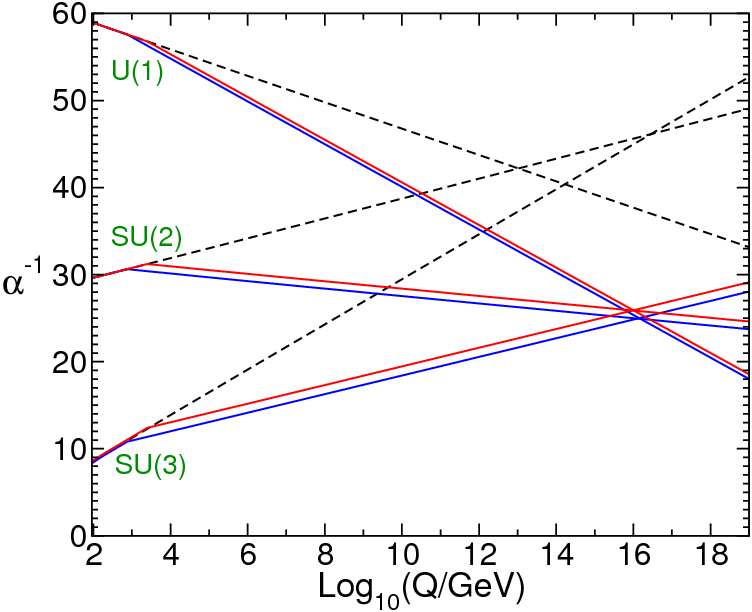
\includegraphics[width=\textwidth]{images/gauge_coupling_unification}
  \caption{2-loop RG evolution of inverse gauge couplings in the SM (dashed lines) and the MSSM (solid lines). The sparticle masses are varied between 0.5-1.5 TeV, and $\alpha_3(m_Z)$ is varied between 0.117 and 0.121. Source: \citep{Martin1997}.}
  \label{fig:gauge_coupling_unification}
\end{marginfigure}

The third major motivation (and the one most relevant to this dissertation) is the fact that the MSSM results in a viable dark matter candidate. The MSSM has a new kind of symmetry known as \emph{R-parity}. It is an analogue of baryon and lepton number conservation. The Lagrangian of the MSSM is defined to be invariant under the action of the operator $P_R$ on the fields. The eigenvalues of this operator are $(-1)^{3(B-L)+2s}$, where \emph{B, L}, and \emph{s} represent the baryon number, lepton number, and spin of the particle, respectively. The consequence of this is that the lightest supersymmetric particle (LSP) must be absolutely stable, that is, it cannot decay further into other particles, thus making it a good candidate for particle dark matter.

The minimal phenomenologically viable incorporation of supersymmetry into the Standard Model is known as the \emph{Minimal Supersymmetric Standard Model}, or the MSSM. However, before describing the salient features of the MSSM, we will outline the construction of a general supersymmetric Lagrangian with all the necessary ingredients we need: kinetic terms, mass terms, scalar self-interactions, gauge symmetry, and Yukawa interactions.

\section{Construction of supersymmetric Lagrangians}
%Symmetries of the S-matrix
In 1967, Coleman and Mandula \citep{Coleman1967} showed that, given certain assumptions, the only possible Lie group symmetries allowed for relativistic interacting field theories in four dimensions are direct products of the Poincar\'e group and an internal symmetry group (i.e. a gauge symmetry) \citep{Mandula2015}.
A Lie algebra is defined by the commutation relations of its generators. If we extend the notion of a Lie algebra to include \emph{anticommutation} relations \citep{Wess1992}, the theorem no longer applies. These kinds of algebras are known as \emph{graded Lie algebras}, or \emph{superalgebras}. The trio of Haag, Łopuszanski, and Sohnius \citep{Haag1975} applied a similar treatment as Coleman and Mandula to determine the most general superalgebra consistent with relativistic quantum field theory. The generators $Q_\alpha$ of this algebra are known as fermionic operators, and must transform as Weyl spinors. The anticommutation (and commutation) relations take the form
\begin{align}
  \begin{split}
  \{Q_\alpha, \bar{Q}_{\dot{\beta}}\} &= 2(\sigma^\mu)_{\alpha\dot{\beta}}P^\mu\\
  \{Q_\alpha, Q_\beta\} &= \{\bar{Q}_{\dot{\alpha}}, \bar{Q}_{\dot{\beta}}\} = 0\\
  [P^\mu,Q_\alpha] &= [P^\mu,\bar{Q}_{\dot{\alpha}}] = 0
\end{split}
\label{eq:susy_algebra}
\end{align}
where $P_\mu = i\partial_\mu$ is the generator of translations. 

The first supersymmetric Lagrangian density in four-dimensions was formulated by Wess and Zumino \citep{Wess1974}. The approach taken was to define infinitesimal `supergauge' transformations for scalars and spinors that generated a closed algebraic structure. Soon afterwards, Salam and Strathdee \citep{Salam1974} created a more systematic approach to constructing these transformations, by giving them a geometric interpretation. In this section, we will outline the construction of a general supersymmetric Lagrangian using the geometric method. The exposition follows that of \citep{Zee2010} and \citep{Martin1997} closely. We make extensive use of the two-component spinor notation - for a review, please see \autoref{ch:notation}.

In the geometric approach, supersymmetric transformations can be viewed as translations in a manifold known as \emph{superspace}, which is obtained by adding the `fermionic' coordinates $\theta^\alpha$, and $\bar{\theta}^{\dot{\beta}}$. Thus, the generators of these translations are represented by
\begin{align}
  Q_\alpha &= \frac{\partial}{\partial\theta^\alpha}-i(\sigma^\mu \bar{\theta})_\alpha \partial_\mu&&\text{and}&&
  \bar{Q}_{\dot{\beta}} = \frac{\partial}{\partial\bar{\theta}^{\dot{\beta}}}-i(\sigma^\mu\bar{\theta})_{\dot{\beta}}\partial_\mu.
\label{eq:susy_operators_diff_form}
\end{align}
These transformations act on objects known as superfields, which are complex scalar fields parameterized by the coordinates $(x^\mu,\theta,\bar{\theta})$
Under an infinitesimal supersymmetry transformation, a general superfield $S(x,\theta,\bar{\theta})$ transforms as
\begin{align}
S\rightarrow S' = (1+i\xi^\alpha Q_\alpha + i\bar{\xi}_{\dot{\alpha}}\bar{Q}^{\dot{\alpha}})S
\label{eq:gen_susy_transformation}
\end{align}
To construct non-supersymmetric Lagrangians, we make use of spacetime derivatives $\partial_\mu$. For supersymmetric Lagrangians, we need an analogue that commutes with supersymmetric transformations. That is, we need an operator $D$ that satisfies the condition $DS' = (DS)'$. This condition can be achieved by defining operators known as \emph{chiral covariant derivatives}, that take the form
\begin{align}
  D_\alpha = \frac{\partial}{\partial\theta^\alpha}+i(\sigma^\mu\bar{\theta})_\alpha\partial_\mu&&\text{ and }&&
  \bar{D}_{\dot{\beta}} = -\left[\frac{\partial}{\partial\bar{\theta}^{\dot{\beta}}}+i(\theta\sigma^\mu)_{\dot{\beta}}\partial_\mu\right]
\end{align}
Using these, we can define a particular kind of superfield, known as a \emph{chiral} superfield and denoted by $\Phi$, that satisfies the constraint $\bar{D}_{\dot{\beta}}\Phi = 0$. One way to implement this constraint is to define a new variable
\[y^\mu=(x^\mu+i\theta^\alpha(\sigma^\mu)_{\alpha\dot{\alpha}}\bar{\theta}^{\dot{\alpha}}).\]
Let us now simplify our notation a bit. For the rest of this section, position four-vectors such as $x^\mu$ will denoted simply by \emph{x}. With this notation, any superfield $\Phi(y,\theta)$ that is a function of only $y$ and $\theta$ will satisfy this constraint, since $\bar{D}_{\dot{\beta}}y = 0$. We perform a Taylor expansion in powers of the variable $\theta$. Now, $\theta$ is a fermionic coordinate, and has two components: $\theta^\alpha = (\theta^1,\theta^2)$. Each of the two components is a \emph{Grassmannian} variable, satisfying the anticommutation relation $\{\theta^i,\theta^i\} = 0$. This implies that $(\theta^i)^2 = 0$. For a general superfield \emph{S}, the Taylor expansion about the fermionic coordinates $\theta,\bar{\theta}$ takes the form
\begin{align}
  \begin{split}
  S(x,\theta,\bar{\theta}) = a &+ \theta\xi + \bar{\theta}\chi^\dagger + \theta\theta b + \bar{\theta}\bar{\theta}c+\bar{\theta}\bar{\sigma}^\mu\theta v_\mu \\
  &+ \bar{\theta}\bar{\theta}\theta\eta + \theta\theta\bar{\theta}\zeta^\dagger+\theta\theta\bar{\theta}\bar{\theta}d,
\end{split}
  \label{eq:general_superfield_expansion}
\end{align}
where \emph{a,b,c} and \emph{d} are complex-valued scalar fields, $\xi,\chi,\eta$ and $\zeta$ are spinor fields, and $v_\mu$ is a vector field. 
For a chiral superfield, after the redefinitions $(a,b,\xi) = (\phi,\sqrt{2}\psi,F)$, the above expansion reduces to
\[\Phi(y,\theta) = \phi(y) + \sqrt{2}\theta\psi(y)+\theta\theta F(y)\]
We can Taylor expand once more around the bosonic coordinate \emph{x} to get
\begin{align}
  \begin{split}
  \Phi(y,\theta) &= \phi(x) + \sqrt{2}\theta\psi(x)+\theta\theta F(x)\\
  &+i\theta\sigma\bar{\theta}\partial_\mu\phi(x)-\frac{1}{2}\theta\sigma\bar{\theta}\theta\sigma^\nu\bar{\theta}\partial_\mu\partial_\nu\phi(x) + \sqrt{2}\theta i\theta\sigma\bar{\theta}\partial_\mu\psi(x)
\end{split}
  \label{eq:superfield_expansion}
\end{align}
Using dimensional analysis, we can extract the forms of the infinitesimal supersymmetric transformations of the fields $\phi,\psi,$ and \emph{F}. The generator $P_\mu$, represents momentum, and has dimensions of mass. We represent this by $[P_\mu] = 1$. Thus, from the supersymmetry algebra (\eqref{eq:susy_algebra}), we have $[Q] = [\bar{Q}] = \slantfrac{1}{2}.$ From the differential forms of \emph{Q} and $\bar{Q}$ in \eqref{eq:susy_operators_diff_form}, we get $[\theta]=[\bar{\theta}]=-\slantfrac{1}{2}$. Since $[\phi] = [\theta\theta]$ and we know that $[\phi] = 1$, we can deduce that $[F]=2$. An infinitesimal supersymmetry transformation changes \emph{F} by an amount $\delta F$, which then must have the same dimensions as \emph{F}. But from the form of the infinitesimal transformation in \eqref{eq:gen_susy_transformation}, we can see that $\delta F$ must be linear in $\xi$ or $\bar{\xi}$, both of which have dimension $\slantfrac{1}{2}$, and so must be multiplied by some object with dimension $\slantfrac{5}{2}$. The only such object available to us from our expansion above is $\partial_\mu\psi$, which is in reality a left-handed Weyl spinor and so carries an undotted index. Multiplying $\partial_\mu\psi^\alpha$ by the object $(\sigma^\mu)_{\alpha\dot{\alpha}}$ allows us to contract the index $\mu$ (ensuring Lorentz invariance), as well as the undotted index $\alpha$. Out of $\xi$ and $\bar{\xi}$, only $\bar{\xi}$ can be used to contract the remaining dotted index. And thus we have, up to an overall constant, $\delta F\sim\bar{\xi}\sigma^\mu\partial_\mu\psi$. It can similarly be argued that $\delta\phi\sim\xi\psi$ and $\delta\psi\sim\xi F+\partial_\mu\phi\sigma^\mu\bar{\xi}$.
The form of $\delta F$ suggests that it is a total divergence, which means that $\int d^4x F$ will be invariant under supersymmetric transformations. We can generalize this result. Let $[\Phi]_F$ denote the coefficient of $\theta\theta$ in the expansion of a superfield $\Phi$. Then $\delta[\Phi]_F$ is a total divergence, and the integral $\int d^4x [\Phi]_F$ is invariant under supersymmetry. The next thing to note is that products of chiral superfields are also superfields: $\Phi^n$ also satisfies the requisite conditions $\bar{D}_{\dot{\beta}}\Phi^n = 0$. So an integral of the form $\int d^4x[W(\Phi)]_F$, where $W(\Phi)$ is a holomorphic \sidefootnote{That is, complex-valued and smooth.} function of the superfield $\Phi$ should also be invariant under supersymmetry. The function $W(\Phi)$ is known as the \emph{superpotential}, and contains the information about the masses and the scalar interactions of of the theory. Now let us add the kinetic terms that make the field dynamical. These terms can be obtained by bringing $\Phi^\dagger$ into the picture, since it will contain the conjugate fields $\bar{\psi}$ necessary to construct kinetic terms such as $\bar{\psi}\bar{\sigma}^\mu\partial_\mu\psi$. A first guess at a superfield that contains both $\Phi$ and $\Phi^\dagger$ is the superfield $V = \Phi^\dagger\Phi$. This field satisfies the property $(\Phi^\dagger\Phi)^\dagger = \Phi^\dagger\Phi$. In general, any superfield $V$ that satisfies the constraint $V = V^\dagger$ is known as a vector superfield.
Recalling the Taylor expansion of $\Phi$ from \eqref{eq:superfield_expansion}, the expansion of \emph{V} in powers of the fermionic coordinates looks like
\[V = \phi^\dagger\phi + 2\bar{\theta}\bar{\psi}\theta\psi + ...\]
The highest power of fermionic coordinates that we can expand to is $\bar{\theta}\bar{\theta}\theta\theta$. Since Grassmannian variables anticommute, the only non-vanishing quadratic combination will be $\bar{\theta}^{\dot{1}}\bar{\theta}^{\dot{2}}\theta_1\theta_2$. Let us follow a similar procedure as with the chiral superfields, and denote the coefficient of $\bar{\theta}\bar{\theta}\theta\theta$ in the expansion of \emph{V} by $[V]_D$. By a dimensional analysis similar to the one performed for the chiral superfields, we can show that $\delta[V]_D$ is a total divergence, and so $\int d^4x[\Phi^\dagger\Phi]_D$ is also supersymmetric. Combining $[\Phi^\dagger\Phi]_D$with our superpotential $W(\Phi)$ from earlier gives us a general supersymmetric Lagrangian:
\begin{align*}
  \mathcal{L} = [\Phi^\dagger\Phi]_D - \left([W(\Phi)]_F + h.c.\right)
\end{align*}
If we choose the superpotential of the form $W(\Phi) = \frac{1}{2}m\Phi^2 + \frac{1}{3}g\Phi^3$ and write the Lagrangian in terms of the component fields $\phi,\psi,F$, we get
\begin{align*}
  \mathcal{L} = (\partial\phi)^\dagger(\partial\phi) + i\bar{\psi}\bar{\sigma}^\mu\partial_\mu\psi+F^\dagger F-\left(mF\phi-\frac{1}{2}m\psi\psi+gF\phi^2-g\phi\psi\psi + \text{h.c.}\right)
\end{align*}
Written like this, it is evident that the component scalar and Weyl spinor fields of a superfield have the same mass, and that $g$ should be viewed as a Yukawa coupling strength. Note that this Lagrangian does not contain any derivatives of the field $F$. This means that it is not a dynamical/propagating field. We refer to $F$ as an \emph{auxiliary} field. We can get rid of of it by `integrating' it out. This can be interpreted in two ways. The first is to perform the path integral over the variables $F$ and $F^\dagger$:
\begin{align*}
\int DFDF^\dagger e^{i\int d^4x \mathcal{L}(\phi,\phi^\dagger,\psi,F,F^\dagger)} = 
 C e^{i\int d^4x \mathcal{L}(\phi,\phi^\dagger,\psi)}
\end{align*}
where $C$ is some constant, which will cancel out in computations of Green's functions, interaction vertices, etc. The other interpretation is that we can exactly solve the Euler-Lagrange equations of motion for the field \emph{F}:
\[\frac{\partial\mathcal{L}}{\partial F}-\partial_\mu\left(\frac{\partial\mathcal{L}}{\partial(\partial_\mu F)}\right) = 0.\]
For our particular Lagrangian, we can collect the terms involving $F$:
\begin{align*}
\mathcal{L}(F) &= F^\dagger F - F(m\phi+g\phi^2) - F^\dagger(m\phi+g\phi^2)^\dagger= |F-(m\phi+g\phi^2)^\dagger|^2
\end{align*}
The Euler-Lagrange equations will be satisfied if $F = (m\phi+g\phi^2)^\dagger$. Thus, after integrating out the auxiliary fields, we get
\begin{align*}
  \mathcal{L}_\text{on-shell} = |\partial\phi|^2+ i\bar{\psi}\bar{\sigma}^\mu\partial_\mu\psi-|m\phi+g\phi^2|+\left(\frac{1}{2}m\psi\psi-g\phi\psi\psi + \text{h.c.}\right)
\end{align*}
We include the hermitian conjugate (h.c.) in the Lagrangian to make the action real.The subscript `on-shell' is an indicator that this Lagrangian is supersymmetric only when the equations of motion are satisfied, i.e. the particles are on-shell. Including the auxiliary fields explicitly in the Lagrangian ensures that the Lagrangian remains supersymmetric even off-shell. So far, we have constructed kinetic terms, mass terms, interactions terms cubic and quartic in the scalar fields $\phi$, and Yukawa terms of the form $\phi\psi\psi$, out of a chiral superfield $\Phi$ and its hermitian conjugate $\Phi^\dagger$. These can be mapped onto the analogous terms in the SM Lagrangian by choosing an appropriate form for the superpotential. The other ingredient we need in this Lagrangian is gauge symmetry, and the corresponding gauge interaction terms.
Just as we obtained the fermion field $\psi$ and the scalar field $\phi$ from the Taylor expansion of a chiral superfield, we can obtain the gauge field $A_\mu^a$ (and its corresponding superpartner $\lambda^a$) from the Taylor expansion of a vector superfield.
For a vector superfield $V(x,\theta,\theta^\dagger)$, the condition $V = V^\dagger$ is equivalent to imposing the constraints
\[a = a^*, \chi^\dagger = \xi^\dagger, c = b^*, v_\mu = v_\mu^*, \zeta^\dagger = \eta^\dagger, d = d^*\]
on the expansion in \eqref{eq:general_superfield_expansion}.
For convenience, we also define:
\begin{align*}
  \eta_\alpha = \lambda_\alpha-\frac{i}{2}(\sigma^\mu\partial_\mu\xi^\dagger)_\alpha&&\text{and}&& d = \frac{1}{2}D+\frac{1}{4}\partial_\mu\partial^\mu a.
\end{align*}
With these constraints and redefinitions, the expansion of the vector superfield takes the form 
\begin{align*}
  V(x,\theta,\theta^\dagger) =& a + \theta\xi + \bar{\theta}\bar{\xi} + \theta\theta b+\bar{\theta}\bar{\theta}b^\dagger + \bar{\theta}\bar{\sigma}^\mu\theta A_\mu + \bar{\theta}\bar{\theta}\theta\left(\lambda-\frac{i}{2}\sigma^\mu\partial_\mu\bar{\xi}\right)\\
  &+\theta\theta\bar{\theta}\left(\lambda^\dagger-\frac{i}{2}\bar{\sigma}^\mu\partial_\mu\xi\right)+\theta\theta\bar{\theta}\bar{\theta}\left(\frac{D}{2}+\frac{1}{4}\partial_\mu\partial^\mu a \right)
\end{align*}
Now let us introduce the concept of \emph{supergauge} transformations. An Abelian example of a supergauge transformation is shown below.
\[V\rightarrow V+i(\Omega^*-\Omega)\]
Here, $\Omega$ is a chiral superfield that parameterizes the transformation.
Using supergauge transformations, we can eliminate the additional auxiliary fields \emph{a,b}, and $\xi$, and write the vector superfield in the \emph{Wess-Zumino} gauge:
\[V_{\text{Wess-Zumino gauge}} = \bar{\theta}\bar{\sigma}^\mu\theta A_\mu + \bar{\theta}\bar{\theta}\theta\lambda+\theta\theta\bar{\theta}\lambda^\dagger + \frac{1}{2}\theta\theta\bar{\theta}\bar{\theta}D\]
By examination, it is evident that if we wish for the field $A_\mu$ to have dimension 1 (like the gauge bosons of the SM), then $V$ must be dimensionless. In this gauge, if $\Lambda$ has an expansion such as the one in \eqref{eq:superfield_expansion}, the vector field $A_\mu$ will transform as
\begin{equation}
A_\mu\rightarrow A_\mu + i\partial_{\mu}(-i\phi^*-i\phi) = A_\mu + \partial_\mu( \text{Re}(\phi))
\label{eq:amu_supergauge_transformation}
\end{equation}
which is simply an Abelian gauge transformation. The presence of the vector field $A_\mu$ is a first hint that interactions mediated by vector bosons involve vector superfields. The field \emph{D} is an auxiliary field, similar to \emph{F}. 
In the SM, we saw that gauge fields $A_\mu$ manifest themselves in the Lagrangian by being present in the kinetic terms (through the covariant derivative) and products of field strength tensors of the form $F^{\mu\nu}F_{\mu\nu}$, where $F_{\mu\nu} = \partial_\mu A_\nu-\partial_\nu A_\mu$.
Before defining the gauge transformation rules for superfields, recall how regular (non-super) fields transform under Abelian gauge symmetries:
\[\phi\rightarrow e^{i\epsilon(x)}\phi\]
where $\epsilon(x)$ is a parameter that is space-time dependent. In fact, $\epsilon(x)$ is simply a scalar field. The supersymmetric generalization of the above transformation for a chiral superfield $\Phi$ is:
\[\Phi\rightarrow e^{2igq\Omega}\Phi\]
where $g$ is the gauge coupling and $q$ is the charge of the field under the symmetry group. The factor of 2 is conventional (to cancel out the 2 in \eqref{eq:amu_supergauge_transformation}, as we shall see). $\Omega$ is a supergauge transformation parameter, and itself a chiral superfield.
To make the kinetic term supergauge-invariant, we modify the kinetic term we had from earlier:
\[[\Phi^\dagger\Phi]_D \rightarrow [\Phi^\dagger e^{2gqV}\Phi]_D\]
where $V$ is a vector field that transforms as in \eqref{eq:amu_supergauge_transformation}. The kinetic term we had earlier, $[\Phi^\dagger\Phi]_D$, is not invariant under supergauge transformations:
\[\Phi^\dagger\Phi\rightarrow e^{-2igq(\Omega^*-\Omega)}\Phi^\dagger\Phi\]
The extra factor can be canceled out if we modify the kinetic term as follows:
\[[\Phi^\dagger\Phi]_D\rightarrow[\Phi^\dagger e^{2gqV}\Phi]_D\]
The field strength corresponding to the vector superfield \emph{V} is
\[\mathcal{W}_\alpha=-\frac{1}{4}\bar{D}\bar{D}D_\alpha V.\]
The supergauge-invariant term in the Lagrangian constructed out of these field strengths is:
\[\frac{1}{4}[\mathcal{W}^\alpha\mathcal{W}_\alpha]_F\]
Putting these terms together\footnote{There is another possible term, which we have omitted, of the form $-2\kappa[V]_D$, which is invariant under supersymmetry and supergauge transformations. This is known as a \emph{Fayet-Iliopoulos} term, and can serve as term that breaks supersymmetry softly.}, the Lagrangian for a theory with an Abelian supergauge invariance takes the form
\begin{equation*}
  \mathcal{L} = \left[\Phi^\dagger e^{2gqV}\Phi\right]_D + \left([W(\Phi)]_F + \text{h.c.}\right) + \frac{1}{4}\left([\mathcal{W}^\alpha\mathcal{W}_\alpha]_F + \text{h.c.}\right)
\end{equation*}
To generalize this to a non-Abelian gauge theory with a set of chiral superfields $\Phi_i$, couplings $g_a$, generators $T^a$ represented by matrices $(T^a)_i^j$, and associated vector superfields $V^a$, we would do the following modifications to the kinetic term and gauge transformation:
\begin{align*}
  [\Phi^\dagger e^{2gqV}\Phi]_D&\rightarrow[\Phi^{i\dagger} (e^{2g_a\mathbf{V}})_i^j\Phi_j]_D\\
  \Phi_i&\rightarrow (e^{i\textbf{Ω}})_i^j\Phi_j
\end{align*}
where the boldfaced symbols are matrices defined by:
\begin{align}
  \mathbf{V} = 2g_aT^aV^a&&\text{and}&& \textbf{Ω} = 2g_aT^a\Omega^a
  \label{eq:matrix_valued_fields}
\end{align}
In this notation, the field strength for \textbf{V} is given by the chiral superfield
\[\mathcal{W}_\alpha = -\frac{1}{2}\bar{D}\bar{D}\left(e^{-\mathbf{V}}D_\alpha e^{\mathbf{V}}\right) = 2g_aT^a\mathcal{W}^a_\alpha\]
Where $\mathcal{W}_\alpha^a$ are the field strengths in adjoint representation - the repeated index \emph{a} is summed over. Finally, putting together all the ingredients, we have a general Lagrangian for a renormalizable supersymmetric field theory including non-Abelian supergauge invariance:
\begin{equation*}
  \mathcal{L} = \left(\frac{1}{4}-\frac{ig_a^2\Theta_a}{32\pi^2}\right)[\mathcal{W}^{a\alpha}\mathcal{W}_{a\alpha}]_F + \text{h.c.} + \left[\Phi^{i\dagger}(e^{\mathbf{V}})\Phi_j\right]_D + \left([W(\Phi)]_F + \text{h.c.}\right)
\end{equation*}
where 
\begin{equation*}
  [\mathcal{W}^{a\alpha}\mathcal{W}_{a\alpha}]_F = \frac{1}{4k_ag_a^2}\text{Tr}[\mathcal{W}^\alpha\mathcal{W}_\alpha]_F
\end{equation*}
Here, $k_a$ defines the normalization of the generators: $\text{Tr}[T^aT^b] = k_a\delta_{ab}$, and is conventionally set to $\slantfrac{1}{2}$. The parameter $\Theta$ is a CP-violating parameter similar to the angle $\theta$ discussed at the beginning of \autoref{ch:2HDMs}. The Fayet-Iliopoulos term that we saw for Abelian supergauge symmetry is no longer allowed since individual terms of the form $-2\kappa[V^a]_D$ are no longer invariant under supergauge transformations - they induce mixing among the vector fields $V^a$ (which is why we worked instead with the matrix-valued fields from \eqref{eq:matrix_valued_fields}).

\section{Chiral and gauge supermultiplets}
Having seen what Lagrangians with supergauge symmetry look like in the superfield and superspace formulation, we can recover regular scalar, vector and spinor fields that are functions of the bosonic coordinates by Taylor expanding the superfields in the Lagrangian. Consider the expansion of a chiral superfield given by
\[\Phi(y,\theta) = \phi(y) + \sqrt{2}\theta\psi(y)+\theta\theta F(y).\]
Choosing values of $\phi,\psi,$ and \emph{F} fixes $\Phi$. Thus, they can be grouped naturally into an object called a \emph{supermultiplet}. In this case, we say that the fields $\phi,\psi,$ and \emph{F} reside in a \emph{chiral} supermultiplet, and that $\phi$ and $\psi$ are superpartners of each other. Recall that an infinitesimal supersymmetry transformation mixes fermionic and bosonic degrees of freedom. Generically, the scalar partner of a fermion is referred to as a \emph{sfermion}. Similarly, recall the expansion of a vector superfield in the Wess-Zumino gauge:
\[V_\text{Wess-Zumino gauge} = \bar{\theta}\bar{\sigma}^\mu\theta A_\mu+\bar{\theta}\bar{\theta}\theta\lambda+\theta\theta\bar{\theta}\lambda^\dagger+\frac{1}{2}\theta\theta\bar{\theta}\bar{\theta}D\]
The fields $A_\mu,\lambda,$ and \emph{D} form another natural grouping, called a \emph{vector} supermultiplet. The fields $A_\mu$ and $\lambda$ are superpartners of each other, and fields such as $\lambda$ are generically known as \emph{gauginos}\footnote{After the co-inventor of the Wess-Zumino model, Bruno Zumino.}.
Let us now take a superpotential of the form:
\begin{equation}
W = \frac{1}{2}M^{ij}\Phi_i\Phi_j + \frac{1}{6}y^{ijk}\Phi_i\Phi_j\Phi_k
\label{eq:superpotential}
\end{equation}
where $M$ is a mass matrix, and $y$ represents the Yukawa couplings and scalar self-interactions.
If we expand the superfields in terms of the component fields, and integrate out the auxiliary fields \emph{F} and \emph{D}, we end up with
\begin{align*}
  \mathcal{L} &= \overbrace{-D^\mu\phi^{\dagger i}D_\mu\phi_i + i\psi^{\dagger i}\bar{\sigma}^\mu D_\mu\psi_i}^\text{kinetic terms}
  -\overbrace{\frac{1}{2}\left\{M^{ij}\psi_i\psi_j+\text{h.c.}\right\}}^{\text{fermion mass terms}}
   +\overbrace{M_{ik}^*M^{kj}\phi^{*i}\phi_j}^\text{scalar mass terms}\\
  &-\overbrace{\frac{1}{2}\left\{y^{ijk}\phi_i\psi_j\psi_k+\text{h.c.}\right\}}^{\text{Yukawa terms}}
  +\overbrace{\frac{1}{2}\left\{M^{in}y_{jkn}^*\phi_i\phi^{*j}\phi^{*k}+\text{h.c.}\right\}}^\text{scalar cubic interactions}\\
  &+\overbrace{\frac{1}{2}g_a^2(\phi^{\dagger i}(T^a)_i^j\phi_j)^2+\frac{1}{4}\left\{y^{ijn}y_{kln}^*\phi_i\phi_j\phi^{*k}\phi^{*l}\right\}}^\text{scalar quartic interactions}\\
  &-\overbrace{\frac{1}{4}F_{\mu}^aF^{\mu\nu a}}^\text{gauge boson self-interactions}
  +\overbrace{i\lambda^{\dagger a}\bar{\sigma}^\mu D_\mu\lambda^a}^\text{gaugino-gauge boson interactions}
\end{align*}

\section{Softly broken supersymmetry}
The component fields of a superfield have the same mass, as can be seen from the mass terms above. This means that, if supersymmetry holds, the superpartners of the SM particles should have been discovered by now. Evidently, if this symmetry exists, it is not evident in the ground state that we inhabit - that is, it must be spontaneously broken. The exact mechanism by which it is broken is still unknown - there are a number of competing models which introduce new physics at high energy scales. To remain model-agnostic, we can simply perform a parameterized explicit breaking by inserting the relevant terms into the Lagrangian by hand. The form of these terms is constrained by the requirement that the quadratic divergences in the radiative corrections to scalar masses must still vanish. With this constraint, we can write a set of generic soft SUSY-breaking terms:

\[\mathcal{L}_\text{soft} = -\left(\frac{1}{2}M_a\lambda^a\lambda^a+\frac{1}{6}a^{ijk}\phi_i\phi_j\phi_k+\frac{1}{2}b^{ij}\phi_i\phi_j+t^i\phi_i\right)+\text{h.c.}-(m^2)_j^i\phi^{j*}\phi_i\]
Note that a general feature of the the above terms is that the masses and couplings have positive mass dimension.

\section{The MSSM}

Specifying a collection of chiral supermultiplets, the gauge symmetry structure, a superpotential of the form in \eqref{eq:superpotential}, and a set of soft SUSY-breaking terms should be enough to reproduce a supersymmetric Lagrangian like the one above. With that in mind, let us put together the ingredients of the MSSM. The first is a gauge symmetry structure, which we will take to be the same as the Standard Model:
\begin{equation*}
  SU(3)_c\times SU(2)_L\times U(1)_Y
\end{equation*}
The next is a set of chiral supermultiplets, and the gauge supermultiplets that correspond to our gauge symmetry structure. These supermultiplets define the particle content of the theory. We show them in \autoref{tab:chiral_supermultiplets} and \autoref{tab:gauge_supermultiplets}, grouped by which group representation they transform under. For brevity, we have not shown all three fermion generations.
\begin{table}
  \caption{Chiral supermultiplets of the MSSM.}
  \label{tab:chiral_supermultiplets}
  \begin{tabular}{cccccc}
    \toprule
                   & \multicolumn{2}{c}{Components}                  & \multicolumn{3}{c}{Group representation} \\ \cmidrule(r){2-3}\cmidrule(l){4-6}
    Superfield     & Spin-0                                          & Spin-$\slantfrac{1}{2}$                                                        & $SU(3)_c$          & $SU(2)_L$    & $U(1)_Y$\\\midrule
                   & Squarks                                         & Quarks                                                                         &                    &              & \\ \cmidrule(r){2-3}\\
    Q              & $\vdoublet{\widetilde{u}_L}{\widetilde{d}_L}$   & $\vdoublet{u_L}{d_L}$                                                          & $\mathbf{3}$       & $\mathbf{2}$ & $\frac{1}{2}$\\\\
    $\overline{u}$ & $\tilde{u}_R^*$                                 & $u_R^\dagger$                                                                  & $\bar{\mathbf{3}}$ & $\mathbf{1}$ & -$\frac{2}{3}$\\\\
    $\overline{d}$ & $\tilde{d}_R^*$                                 & $d_R^\dagger$                                                                  & $\bar{\mathbf{3}}$ & $\mathbf{1}$ & $\frac{1}{3}$\\\\\cmidrule{2-3}
                   & Sleptons                                        & Leptons                                                                        &                    &              & \\ \cmidrule{2-3}\\
    \emph{L}       & $\vdoublet{\widetilde{\nu}_L}{\widetilde{e}_L}$ & $\vdoublet{\nu_L}{e_L}$                                                        & $\mathbf{1}$       & $\mathbf{2}$ & -$\frac{1}{2}$\\\\
    $\overline{e}$ & $\tilde{e}_R^*$                                 & $e_R^\dagger$                                                                  & $\bar{\mathbf{1}}$ & $\mathbf{1}$ & $1$\\\\\cmidrule{2-3}
                   & Higgses                                         & Higgsinos                                                                      &                    &              & \\ \cmidrule{2-3}\\
    $H_u$          & $\vdoublet{H_u^+}{H_u^0}$                       & $\vdoublet{\widetilde{H}_u^+}{\widetilde{H}_u^0}$                              & $\mathbf{1}$       & $\mathbf{2}$ & $\frac{1}{2}$\\\\
    $H_d$          & $\vdoublet{H_d^0}{H_d^-}$                       & $\vdoublet{\widetilde{H}_d^0}{\widetilde{H}_d^-}$                              & $\mathbf{1}$       & $\mathbf{2}$ & -$\frac{1}{2}$\\\\
    \bottomrule
  \end{tabular}
\end{table}

\begin{table}
  \caption{Gauge supermultiplets of the MSSM.}
  \label{tab:gauge_supermultiplets}
  \begin{tabular}{ccccc}
    \toprule
\multicolumn{2}{c}{Components} & \multicolumn{3}{c}{Group representation} \\ \cmidrule(r){1-2}\cmidrule(l){3-5}
Spin-$\slantfrac{1}{2}$        & Spin-1                                                                         & $SU(3)_c$          & $SU(2)_L$    & $U(1)_Y$\\\midrule
Gluinos: $\widetilde{g}$       & Gluons: \emph{g}                                                               & $\mathbf{8}$       & $\mathbf{1}$ & 0 \\\\
Winos: $\widetilde{W}^0$       & W bosons: $W^\pm$                                                              & $\bar{\mathbf{1}}$ & $\mathbf{3}$ & 0\\\\
Binos: $\widetilde{B}^0$       & B bosons: $B^0$                                                                & $\bar{\mathbf{1}}$ & $\mathbf{3}$ & 0\\
    \bottomrule
  \end{tabular}
\end{table}
Next, let us specify the superpotential. In terms of the chiral superfields in \autoref{tab:chiral_supermultiplets}, we can write the MSSM superpotential as:
\[W_\text{MSSM} = \bar{u}\mathbf{y_u}QH_u-\bar{d}\mathbf{y_d}Q H_d-\bar{e}\mathbf{y_e}L H_d+\mu H_u H_d \]
where we have abbreviated terms such as $\mu(H_u)_\alpha (H_d)_\beta\epsilon^{\alpha\beta}$ to $\mu H_u H_d$, and the matrices $\mathbf{y}$ are $3\times3$ matrices of Yukawa couplings, with indices representing the fermion generations. 
Note also that we now see the necessity of having two Higgs doublets - one that couples to the up-type fermions, and the other to the down-type fermions. A term like $\overline{u}\mathbf{y_u}QH_d^*$ would lead to a non-conserved hypercharge.
Finally, we have a set of terms that soft SUSY-breaking terms.
\begin{align*}
  \begin{split}
    \mathcal{L}_\text{soft}^\text{MSSM} &= -\frac{1}{2}\left(M_1\tilde{B}\tilde{B}+
    M_2\widetilde{W}\widetilde{W} + M_3\widetilde{g}\widetilde{g} + \text{h.c.}\right)\\
    &-\left(\widetilde{\overline{u}}\mathbf{a_u}\widetilde{Q}H_u-\widetilde{\overline{d}}\mathbf{a_d}-\widetilde{\overline{e}}\mathbf{a_e}\widetilde{L}H_d+\text{h.c.}\right)\\
    &-\widetilde{Q}^\dagger\mathbf{m_Q^2}\widetilde{Q}
     -\widetilde{L}^\dagger\mathbf{m_L^2}\widetilde{L}
     -\widetilde{\overline{u}}^\dagger\mathbf{m_{\overline{u}}^2}\widetilde{\overline{u}}^\dagger
     -\widetilde{\overline{d}}^\dagger\mathbf{m_{\overline{d}}^2}\widetilde{\overline{d}}^\dagger
     -\widetilde{\overline{e}}^\dagger\mathbf{m_{\overline{e}}^2}\widetilde{\overline{e}}^\dagger
  \end{split}
\end{align*}
\subsection{Phenomenological approximations}
Often, the MSSM has a number of simplifying assumptions motivated both by convenience and compatibility with observed experimental data. For example, it is convenient to take the Yukawa matrices $\mathbf{y_u,y_d,y_e}$ in a simplified limit, where only the heaviest generations have non-zero Yukawa couplings. 
\begin{align*}
  \mathbf{y_u} \approx \begin{pmatrix}
    0 & 0 & 0\\
    0 & 0 & 0\\
    0 & 0 & y_t
  \end{pmatrix},&&
  \mathbf{y_d} \approx \begin{pmatrix}
    0 & 0 & 0\\
    0 & 0 & 0\\
    0 & 0 & y_b
  \end{pmatrix},&&
  \mathbf{y_e} \approx \begin{pmatrix}
    0 & 0 & 0\\
    0 & 0 & 0\\
    0 & 0 & y_\tau
  \end{pmatrix}
\end{align*}
Furthermore, to suppress excessive CP-violation and FCNCs in the MSSM, the following approximations are often made:
\begin{align*}
  \mathbf{m_Q^2} = m_Q^2\mathbf{1},&&
  \mathbf{m_{\bar{u}}^2} = m_{\bar{u}}^2\mathbf{1},&&
  \mathbf{m_{\bar{d}}^2} = m_{\bar{d}}^2\mathbf{1},&&
  \mathbf{m_{\bar{e}}^2} = m_{\bar{e}}^2\mathbf{1},&&
  \mathbf{m_{\bar{L}}^2} = m_{\bar{L}}^2\mathbf{1}\\
\end{align*}
\begin{align*}
  \mathbf{a_u} = A_{u0}\mathbf{y_u},&&
  \mathbf{a_d} = A_{d0}\mathbf{y_d},&&
  \mathbf{a_e} = A_{e0}\mathbf{y_e}\\
\end{align*}
\begin{align*}
  \text{Im}(M_1)=
  \text{Im}(M_2)=
  \text{Im}(M_3)=
  \text{Im}(A_{u0})=
  \text{Im}(A_{d0})=
  \text{Im}(A_{e0})=0
\end{align*}
With the above ingredients, one can work out myriad phenomenological consequences. In \autoref{ch:DM_100_TeV}, we examine the neutralino sector of the MSSM in slightly more detail.

\section{Split Supersymmetry}
This paradigm, known as `natural' supersymmetry  has been the dominant paradigm for constructing supersymmetric models for decades. However, recent data from the LHC has placed severe constraints on this picture. With this in mind, it is worth considering what would happen if we relaxed the criterion of `naturalness'. More specifically, a spectrum with a mass hierarchy between the scalar and fermionic superpartners of the SM particles - anywhere on the order of 10-100 TeV - offers a number of benefits, at the cost of some level of fine-tuning. Such a spectrum is called a \emph{split} spectrum. This idea was first introduced in \citep{Wells:2003tf,Arkani-Hamed2005,Giudice2005}, and might well take the crown from natural supersymmetry as the dominant paradigm in the decades to follow. In \autoref{ch:DM_100_TeV}, we examine a split spectrum with the hierarchy $M_1 < |\mu| << M_2$. and a strategy to probe the split parameter space at a 100 TeV collider.

\chapter{Collider Phenomenology and Machine Learning}\label{ch:ColliderPheno}
In this chapter, we will discuss how to connect theory and experiment. We will begin by connecting scattering amplitudes and physically observed cross sections, after which we will briefly discuss detector components of the LHC, and then move on to the question of how we establish statistical significance given experimental data from detectors.

% Scattering amplitudes and cross sections
To observe physics at subatomic length scales, it is necessary to produce interactions on those scales. This requires colliding particles at speeds close to the speed of light. The energy of these collisions is so high that not only do the colliding particles scatter off of each other, but new particles can be created as well. 
The physical observable at particle colliders is a quantity known as the scattering cross section, denoted by $\sigma$. It is defined by the relation
\[R = \sigma\mathcal{L}\]
where \emph{R} is the rate of collisions per unit time, and $\mathcal{L}$ is the luminosity of the collider, that is, the number of particles passing through some cross-sectional area per unit time. The scattering cross-section $\sigma$ for a generic process with particles 1 and 2 colliding to produce a set of particles \emph{X} as the final state is given by the integral of the scattering amplitude for the process, $|\mathcal{M}_{12\rightarrow X}|^2$ over the phase space of \emph{X}\footnote{Here we omit the form factors that would come into play at a hadronic collider, without affecting our narrative.}. 
\begin{equation}
  \sigma_{12} = \int d\Pi_X |\mathcal{M}_{12\rightarrow X}|^2
\end{equation}
The dynamics of the collision event are contained in the matrix element $\mathcal{M}$, which will be influenced by the presence of BSM physics.
Thus, the typical quantities of interest are the \emph{differential} cross sections, $d\sigma/dx$, where \emph{x} represents some kinematic variable. 
Particle colliders are broadly categorized as either lepton or hadron colliders. Each one has its advantages and disadvantages. Lepton colliders have cleaner signals than hadron colliders due to the lack of large QCD backgrounds. On the other hand, hadron colliders are able to reach much larger center-of-mass energies, since leptons lose large amounts of energy via synchrotron radiation when forced along a circular path. In this work, we will focus on the phenomenology of hadron colliders, both present and future.
\section{Detector design for hadron colliders}
Particle detectors can be thought of as sophisticated videocameras with extremely high framerates. Conversely, the digital cameras that we use in our daily lives can be thought of as particle detectors, except designed for only one kind of particle, the photon. The response of a detector to an incident particle can take on a variety of forms. In a gaseous detector such as a  Geiger-Muller tube, an energetic incident particle will lead to the ionization of a large fraction of the gas molecules, followed by rapid recombination. This is manifested as an electrical pulse. The analogue of ionization for a solid-state detector (such as the ones used in regular digital cameras) is the creation of a large number of electron-hole pairs. The design of a particle detector will be based upon the particles it aims to detect as well as the desired precision and accuracy.
At the Large Hadron Collider at CERN, the two major detectors are ATLAS (A Toroidal LHC Apparatus) and CMS (Compact Muon Solenoid). They differ slightly in construction, but essentially probe the same physics. The components common to them are the following.
\paragraph{Tracking chamber}
The innermost part of the detector is the tracking chamber. It consists of layers of solid-state detectors that can accurately measure the paths of charged particles that are formed in the particle collision events. The presence of a strong magnetic field bends the paths of these particles, enabling us to learn about their charge and mass.
\paragraph{Calorimeter(s)}
If a particle is energetic enough to go beyond the tracking chamber, it enters the calorimeter region. A calorimeter consists of materials dense enough to completely absorb the energy of an incident particle and stop it in its tracks. At ATLAS and CMS, the calorimeter is actually a combination of two layers that are designed to stop different kinds of particles. The electromagnetic calorimeter is designed to measure the energy of electrons and photons, while the hadronic calorimeter is designed to stop (and you might have guessed this already) hadrons. 
\paragraph{Muon Detectors} The muon, being about 200 times heavier than the electron, experiences much less energy loss through bremsstrahlung, and is able to bypass both the tracking chamber and calorimeter layers. For this reason, muon detectors form the outermost layer of a particle detector.

A transverse slice of the CMS detector is shown in \autoref{fig:CMS_slice}, depicting the trajectories taken by different kinds of particles through the layers of the detector.
The specific design of a detector depends upon the vision of the collaboration running it. With a finite construction and operation budget, tradeoffs must inevitably be made. Although ATLAS and CMS are both state of the art multipurpose detectors, they have their strengths and weaknesses relative to each other based upon different sets of priorities. For this reason, we do not provide the specifics of their construction, and instead point the reader to \citep{Froidevaux2006} for a detailed review and comparison of the two.
For our purposes, the features of the collision events that we use to perform our analyses (particle momentum, missing transverse energy, etc.) can be measured with either of these detectors.
\begin{figure}
  \begin{sidecaption}
    {Transverse slice of the CMS detector, showing the paths of various particles. Source: \citep{CMS_Slice}}[fig:CMS_slice]
    \centering
    \includegraphics[trim={0 0 0 4cm},clip,width=\textwidth]{images/CMS_slice}
  \end{sidecaption}
\end{figure}
\paragraph{Trigger} As mentioned in \autoref{ch:introduction}, there are hundreds of millions of collisions every second at the LHC. Recording and analyzing all of these events would be impractical, given that most of the collisions simply involve small deflections. What we are really interested in are the \emph{hard} collisions, with the final state particles having a high amount of momentum in the transverse plane. To filter out the uninteresting events, we employ a \emph{trigger} - that is, a condition that an event must satisfy to be stored for further analysis. For example, in \autoref{ch:DM_100_TeV}, we choose to trigger on a hard lepton, that is, one with a high transverse momentum.
\paragraph{Invisibles} An important point to note is that certain particles, such as neutrinos and dark matter candidates, escape the detector entirely, leaving no tracks or energy deposits. The existence of one of these `invisible' particles in a collision event can only be inferred from an observed imbalance of momenta of the final state particles in the transverse direction. Thus, for analyses involving neutrinos or dark matter, the kinematic quantity known as \emph{missing transverse energy}, denoted by $\slashed{E}_T$, is of utmost importance.

\section{Anatomy of a collider analysis}
At its heart, the goal of a collider analysis is to compare the predictions of the SM and BSM theories with actual experimental data, and estimate the level of compatibility between them. To do this well, we need precise theoretical predictions of the differential cross sections that we can expect to see at the collider. This is done with the help of Monte Carlo methods and detector simulations, as described below. 
\subsection{Parton-level event generation}
As mentioned earlier, the cross section for a scattering process is an integral of the scattering amplitude over the phase space of the final state particles. 
In general, these integrals do not have a closed form solution, and so we must resort to numerical integration. The simplest Monte Carlo integration method, the \emph{acceptance-rejection} method, involves randomly sampling points within the limits of integration with a uniform probability distribution, and testing whether they lie under the `curve' specified by the integrand. The fraction of points that pass this test, multiplied by the volume of this `bounding box' specified by the integration limits, gives the definite integral. This method is difficult to view in multiple dimensions, but not too hard to grasp in one or two dimensions - see \citep{Pyarelal2011} for a brief overview and implementation. However, drawing the random samples from a uniform probability distribution is not the most efficient method for performing Monte Carlo integrals - programs such MadGraph5 and MadEvent \citep{Alwall2014} do this in more sophisticated ways, determining the roughly most important regions of phase space and concentrating the sampling within those regions. These `points' are simply the particle collision events themselves, with coordinates given by the four-momenta of the final state particles. 
\subsection{Showering and hadronization}
At hadron colliders, dealing with the matrix element $\mathcal{M}$ alone will not suffice. We must also take into account nonperturbative QCD effects, such as the radiation of soft gluons, and the formation of complex hadronic final states. For example, even if an energetic quark is contained in an event generated by MadEvent, it will not be detected as an elementary particle. It will radiate gluons that themselves split to form new quarks, that subsequently form bound states. This collection of hadronic bound states is termed a jet, and has a momentum collinear with the momentum of the original quark. The identity of this quark can be determined (with a finite efficiency) from the properties of the jet. To handle these non-perturbative effects, we interface MadEvent with the program Pythia\citep{Sjostrand2006} which performs the steps of parton showering and hadronization.
\subsection{Detector simulation and reconstruction}
A full collider analysis carried out by experimentalists will involve detailed simulations of the detector response, using programs such as GEANT4 \citep{Agostinelli2003}. For our purposes, however, it is enough to parameterize the detector response at a higher level - for example, specifying a fixed probability for identifying a certain particle. This is done using the Delphes 3 framework \citep{DeFavereau2014a}, which provides a way to perform a fast, modular simulation of the detector response. 

\subsection{Hypothesis testing}
After signal and background samples have been generated using Monte Carlo methods and passed through a detector simulation, they are compared to actual experimental data. Doing this enables us to do one or more of the following:
\begin{itemize}
  \item Estimate some parameter, for example the mass of a particle, or a coupling strength.
  \item Set upper limits on the rate of occurrence of a process, and translating those limits into limits on the parameter space of BSM theories.
  \item Discover a new particle
  \item Compare theoretical and experimental differential cross sections using a goodness-of-fit test.
\end{itemize}
As it turns out, all of these can be subsumed into the larger framework of \emph{hypothesis testing} \citep{Heinrich}. 
%In our case, we most interested in discovering new particles, or failing that, excluding regions of parameter space for BSM theories.
In the following section, we will address how we answer the question ``Does this experimental data imply the existence of new physics (or conversely, rule it out) ?". This discussion is adapted from the one in \citep{Cranmer2015}. 

\section{Statistical significance in particle physics}
A hypothesis is a claim about what the experimental data will look like, given some model parameters. Let us consider hypothesis testing in the context of a simple counting experiment, in the frequentist interpretation. In this experiment, we examine the subset of a dataset $\mathcal{D}$ that resides in a region of the `data space' labeled the \emph{signal region} (SR), and contains $n_{SR}$ events. Our competing hypotheses are the `background-only' and `signal plus background' hypotheses, described in \autoref{tab:hypotheses}. 
\begin{table}
  \begin{sidecaption}{The two competing hypotheses for our simple number counting example. Source: \cite{Cranmer2015}.}[tab:hypotheses]
  \begin{tabular}{llll}
    \toprule
    Symbol & Statistical name & Physics name & Probability model\\
    \midrule
    $H_0$ & Null & Background-only & Pois($n_{SR}|\nu_B$)\\
    $H_1$ & Alternate & Signal+Background & Pois($n_{SR}|\nu_S+\nu_B$)\\
    \bottomrule
  \end{tabular}
\end{sidecaption}
\end{table}
The probability models associated with these hypotheses are Poisson models\footnote{The exact probabiliity distribution for counting experiments is given by the binomial frequency function. In the limit of a large number of events, this approaches the Poisson frequency function, given by
  \[\text{Pois}(n|\nu) = \nu^n\frac{e^{-\nu}}{n!}\]
  which describes the probability of observing \emph{n} events given that the mean expected number of events is $\nu$.
}. The model for the 'background-only' hypothesis is Pois$(n_{SR}|\nu_B)$, that is, the probability of obtaining $n_{SR}$ events in the signal region when $\nu_B$ events are expected from the background process. The competing hypothesis, `signal plus background', on the other hand, predicts $\nu_S+\nu_B$ events in the signal region, with $\nu_S$ events from the signal process and $\nu_B$ events from the background process. The probability that the background-only hypothesis will produce at least $n_\text{SR}$ events is given by
\[p_\text{background only} = \sum_{n=n_\text{SR}}^\infty \text{Pois}(n|\nu_B)\]
The lower this probability is, the less likely it is that the background-only hypothesis can account for the observed number of events in the signal region. This quantity is also known colloquially as the \emph{p}-value - in this case, it is the \emph{p}-value for the background-only hypothesis. The corresponding \emph{p}-value for the signal + background hypothesis is given by:
\[p_\text{signal + background} = \sum_{n=n_\text{SR}}^\infty \text{Pois}(n|\nu_S + \nu_B)\]
For phenomenology, there are usually two \emph{p}-value thresholds of interest. The first is the exclusion threshold - if $p_\text{signal + background} < 0.05$, we consider the signal + background hypothesis `excluded'. The second is the discovery criterion, $p_\text{background only} < 2.87\times 10^{-7}$. When this condition is satisfied, we choose to reject the background-only hypothesis, and claim discovery of new physics. In practice, \emph{p}-values are reported in terms of equivalent \emph{Z}-values. The \emph{Z} value corresponding to a \emph{p}-value $p_0$ is given by
\[Z = \Phi^{-1}(1-p_0)\]
where $\Phi^{-1}$ is the inverse of the cumulative distribution function of the standard normal distribution (a Gaussian distribution with mean 0 and variance 1). The equivalent \emph{Z}-values for the exclusion and discovery \emph{p}-value thresholds are 1.96 and 5, respectively. In particle physics parlance, the equivalent \emph{Z} value is known as the \emph{significance}, and is reported as $Z\sigma$.
The significance is maximized by choosing signal regions with low values of $\nu_B$.
This can be seen from the expressions for $p_\text{background only}$. Lower values of $\nu_B$ lead to lower values of $p_\text{background only}$, minimizing the probability, denoted $\alpha$, that we will wrongly reject the background-only hypothesis when it is true. This is known as a Type-I error. However, in general, there can be multiple, or even an infinite number of such regions in data space. Moreover, this criterion does not let us say anything about the signal + background hypothesis. Thus, we also require that the choice of the signal region leads to a low probability (denoted $\beta$) of wrongly accepting the background-only hypothesis when the signal + background hypothesis is true (a Type-II error).

In the language of hypothesis testing, then, the job of a collider phenomenologist like myself is to find regions of data space that \emph{minimize} the probability of wrongly accepting the null hypothesis when the alternate hypothesis is true, given a \emph{fixed} probability of wrongly rejecting the null hypothesis when the alternate hypothesis is true.

Whew, that is a mouthful! In more concise terms, we would like to minimize $\beta$ for a given value of $\alpha$. The quantity $\alpha$ is known as the \emph{size} of the test, and the quantity $1-\beta$ is known as the \emph{power} of the test. And more importantly, in practical terms, this task boils down to finding regions of the data space that are densely populated by signal events (minimizing $\beta$) and sparsely populated by background events (minimizing $\alpha$). After isolating a promising signal region, we calculate the maximum achievable value of \emph{Z}. In general, the value of \emph{Z} will be calculated differently for claiming exclusion or discovery. However, we are not performing a full collider analysis, but rather a sort of `feasibility study', for which we simply use the asymptotic formula for \emph{Z} obtained by taking limit in which the probability distributions are Gaussian, and the signal rates are much smaller than the background rates.
\[Z \approx \frac{n_S}{\sqrt{n_B}}\]
where $n_S$ and $n_B$ are the number of signal and background events observed in the signal region respectively.

Traditionally, promising signal regions are found by formulating kinematic variables that can efficiently discriminate between signal and background events. These variables are designed based on our knowledge of the kinematics of the final state particles in the signal and background events. They include variables such as invariant mass, missing transverse energy, and transverse mass. While this approach has served us well so far, the models being examined are grown increasingly complex, with large parameter spaces, and with the increase in collision energy comes a much larger rate of background event production. The boundary of the optimal signal region in data space, can potentially be highly non-linear. The traditional `cut-and-count' strategy finds the signal region by applying a series of one or two dimensional selection cuts on the data. This approach can potentially miss higher-dimensional correlations in the data space. These correlations can be found efficiently through the use of \emph{machine learning} techniques, which we discuss in \autoref{sec:MachineLearning}.

\paragraph{Reach in parameter space} As mentioned earlier, new physics theories such as Two Higgs Doublet Models can have extremely large parameter spaces. Each point of a theory's parameter space can be considered as a new physics hypothesis. In our analyses, we aim to perform hypothesis tests for a large number of points in parameter space, and ascertain which of the points, or hypotheses, can be rejected, or alternatively, discovered. Doing this, we find contours of the the equivalent \emph{Z} values in the parameter space. Typically we show only the contours for $Z = 1.96$ and $Z=5$, that is, the discovery and exclusion contours. We term the area bounded by these contours the \emph{reach} of our analysis in parameter space. 

\section{Machine learning in particle physics}\label{sec:MachineLearning}
Separating signals and backgrounds in particle physics is, in the language of machine learning, a \emph{classification} problem. One can consider particle collision events as residing in a space, where the coordinates of each event are represented by various \emph{features} of the event. This is equivalent to the `data space' discussed in the previous section. These features could be high-level ones such as invariant masses, or low-level ones, such as the momentum components of individual final state particles. What we do when we perform a cut-and-count analysis is to try and isolate a region of this space that is rich in signal events. Typically, the most straightforward approach is to define a sort of `box' in feature space using rectangular, one-dimensional cuts. However, there is no guarantee that signal events are confined to such a box --- correlations between the features can distort the distribution of events in feature space. 
\strictpagecheck
\begin{figure}
  \begin{sidecaption}{Illustration of a non-linear decision boundary in two-dimensional feature space.}[fig:nonlinear_decision_boundary]
  %% Creator: Matplotlib, PGF backend
%%
%% To include the figure in your LaTeX document, write
%%   \input{<filename>.pgf}
%%
%% Make sure the required packages are loaded in your preamble
%%   \usepackage{pgf}
%%
%% Figures using additional raster images can only be included by \input if
%% they are in the same directory as the main LaTeX file. For loading figures
%% from other directories you can use the `import` package
%%   \usepackage{import}
%% and then include the figures with
%%   \import{<path to file>}{<filename>.pgf}
%%
%% Matplotlib used the following preamble
%%   \usepackage{fontspec}
%%   \setmainfont{Minion Pro}
%%   \setsansfont{Lucida Grande}
%%   \setmonofont{Andale Mono}
%%
\begingroup%
\makeatletter%
\begin{pgfpicture}%
\pgfpathrectangle{\pgfpointorigin}{\pgfqpoint{3.880000in}{3.880000in}}%
\pgfusepath{use as bounding box, clip}%
\begin{pgfscope}%
\pgfsetbuttcap%
\pgfsetmiterjoin%
\definecolor{currentfill}{rgb}{0.941176,0.941176,0.941176}%
\pgfsetfillcolor{currentfill}%
\pgfsetlinewidth{0.000000pt}%
\definecolor{currentstroke}{rgb}{0.941176,0.941176,0.941176}%
\pgfsetstrokecolor{currentstroke}%
\pgfsetdash{}{0pt}%
\pgfpathmoveto{\pgfqpoint{0.000000in}{0.000000in}}%
\pgfpathlineto{\pgfqpoint{3.880000in}{0.000000in}}%
\pgfpathlineto{\pgfqpoint{3.880000in}{3.880000in}}%
\pgfpathlineto{\pgfqpoint{0.000000in}{3.880000in}}%
\pgfpathclose%
\pgfusepath{fill}%
\end{pgfscope}%
\begin{pgfscope}%
\pgfsetbuttcap%
\pgfsetmiterjoin%
\definecolor{currentfill}{rgb}{0.941176,0.941176,0.941176}%
\pgfsetfillcolor{currentfill}%
\pgfsetlinewidth{0.000000pt}%
\definecolor{currentstroke}{rgb}{0.000000,0.000000,0.000000}%
\pgfsetstrokecolor{currentstroke}%
\pgfsetstrokeopacity{0.000000}%
\pgfsetdash{}{0pt}%
\pgfpathmoveto{\pgfqpoint{0.511667in}{0.504167in}}%
\pgfpathlineto{\pgfqpoint{3.730000in}{0.504167in}}%
\pgfpathlineto{\pgfqpoint{3.730000in}{3.730000in}}%
\pgfpathlineto{\pgfqpoint{0.511667in}{3.730000in}}%
\pgfpathclose%
\pgfusepath{fill}%
\end{pgfscope}%
\begin{pgfscope}%
\pgfpathrectangle{\pgfqpoint{0.511667in}{0.504167in}}{\pgfqpoint{3.218333in}{3.225833in}} %
\pgfusepath{clip}%
\pgfsetbuttcap%
\pgfsetroundjoin%
\pgfsetlinewidth{1.003750pt}%
\definecolor{currentstroke}{rgb}{0.796078,0.796078,0.796078}%
\pgfsetstrokecolor{currentstroke}%
\pgfsetdash{}{0pt}%
\pgfpathmoveto{\pgfqpoint{0.686291in}{0.504167in}}%
\pgfpathlineto{\pgfqpoint{0.686291in}{3.730000in}}%
\pgfusepath{stroke}%
\end{pgfscope}%
\begin{pgfscope}%
\pgftext[x=0.686291in,y=0.455556in,,top]{\rmfamily\fontsize{10.000000}{12.000000}\selectfont 0}%
\end{pgfscope}%
\begin{pgfscope}%
\pgfpathrectangle{\pgfqpoint{0.511667in}{0.504167in}}{\pgfqpoint{3.218333in}{3.225833in}} %
\pgfusepath{clip}%
\pgfsetbuttcap%
\pgfsetroundjoin%
\pgfsetlinewidth{1.003750pt}%
\definecolor{currentstroke}{rgb}{0.796078,0.796078,0.796078}%
\pgfsetstrokecolor{currentstroke}%
\pgfsetdash{}{0pt}%
\pgfpathmoveto{\pgfqpoint{1.349639in}{0.504167in}}%
\pgfpathlineto{\pgfqpoint{1.349639in}{3.730000in}}%
\pgfusepath{stroke}%
\end{pgfscope}%
\begin{pgfscope}%
\pgftext[x=1.349639in,y=0.455556in,,top]{\rmfamily\fontsize{10.000000}{12.000000}\selectfont 5}%
\end{pgfscope}%
\begin{pgfscope}%
\pgfpathrectangle{\pgfqpoint{0.511667in}{0.504167in}}{\pgfqpoint{3.218333in}{3.225833in}} %
\pgfusepath{clip}%
\pgfsetbuttcap%
\pgfsetroundjoin%
\pgfsetlinewidth{1.003750pt}%
\definecolor{currentstroke}{rgb}{0.796078,0.796078,0.796078}%
\pgfsetstrokecolor{currentstroke}%
\pgfsetdash{}{0pt}%
\pgfpathmoveto{\pgfqpoint{2.012986in}{0.504167in}}%
\pgfpathlineto{\pgfqpoint{2.012986in}{3.730000in}}%
\pgfusepath{stroke}%
\end{pgfscope}%
\begin{pgfscope}%
\pgftext[x=2.012986in,y=0.455556in,,top]{\rmfamily\fontsize{10.000000}{12.000000}\selectfont 10}%
\end{pgfscope}%
\begin{pgfscope}%
\pgfpathrectangle{\pgfqpoint{0.511667in}{0.504167in}}{\pgfqpoint{3.218333in}{3.225833in}} %
\pgfusepath{clip}%
\pgfsetbuttcap%
\pgfsetroundjoin%
\pgfsetlinewidth{1.003750pt}%
\definecolor{currentstroke}{rgb}{0.796078,0.796078,0.796078}%
\pgfsetstrokecolor{currentstroke}%
\pgfsetdash{}{0pt}%
\pgfpathmoveto{\pgfqpoint{2.676333in}{0.504167in}}%
\pgfpathlineto{\pgfqpoint{2.676333in}{3.730000in}}%
\pgfusepath{stroke}%
\end{pgfscope}%
\begin{pgfscope}%
\pgftext[x=2.676333in,y=0.455556in,,top]{\rmfamily\fontsize{10.000000}{12.000000}\selectfont 15}%
\end{pgfscope}%
\begin{pgfscope}%
\pgfpathrectangle{\pgfqpoint{0.511667in}{0.504167in}}{\pgfqpoint{3.218333in}{3.225833in}} %
\pgfusepath{clip}%
\pgfsetbuttcap%
\pgfsetroundjoin%
\pgfsetlinewidth{1.003750pt}%
\definecolor{currentstroke}{rgb}{0.796078,0.796078,0.796078}%
\pgfsetstrokecolor{currentstroke}%
\pgfsetdash{}{0pt}%
\pgfpathmoveto{\pgfqpoint{3.339680in}{0.504167in}}%
\pgfpathlineto{\pgfqpoint{3.339680in}{3.730000in}}%
\pgfusepath{stroke}%
\end{pgfscope}%
\begin{pgfscope}%
\pgftext[x=3.339680in,y=0.455556in,,top]{\rmfamily\fontsize{10.000000}{12.000000}\selectfont 20}%
\end{pgfscope}%
\begin{pgfscope}%
\pgftext[x=2.120833in,y=0.267778in,,top]{\rmfamily\fontsize{10.000000}{12.000000}\selectfont Feature One}%
\end{pgfscope}%
\begin{pgfscope}%
\pgfpathrectangle{\pgfqpoint{0.511667in}{0.504167in}}{\pgfqpoint{3.218333in}{3.225833in}} %
\pgfusepath{clip}%
\pgfsetbuttcap%
\pgfsetroundjoin%
\pgfsetlinewidth{1.003750pt}%
\definecolor{currentstroke}{rgb}{0.796078,0.796078,0.796078}%
\pgfsetstrokecolor{currentstroke}%
\pgfsetdash{}{0pt}%
\pgfpathmoveto{\pgfqpoint{0.511667in}{0.681280in}}%
\pgfpathlineto{\pgfqpoint{3.730000in}{0.681280in}}%
\pgfusepath{stroke}%
\end{pgfscope}%
\begin{pgfscope}%
\pgftext[x=0.396389in,y=0.631836in,left,base]{\rmfamily\fontsize{10.000000}{12.000000}\selectfont 0}%
\end{pgfscope}%
\begin{pgfscope}%
\pgfpathrectangle{\pgfqpoint{0.511667in}{0.504167in}}{\pgfqpoint{3.218333in}{3.225833in}} %
\pgfusepath{clip}%
\pgfsetbuttcap%
\pgfsetroundjoin%
\pgfsetlinewidth{1.003750pt}%
\definecolor{currentstroke}{rgb}{0.796078,0.796078,0.796078}%
\pgfsetstrokecolor{currentstroke}%
\pgfsetdash{}{0pt}%
\pgfpathmoveto{\pgfqpoint{0.511667in}{1.298496in}}%
\pgfpathlineto{\pgfqpoint{3.730000in}{1.298496in}}%
\pgfusepath{stroke}%
\end{pgfscope}%
\begin{pgfscope}%
\pgftext[x=0.396389in,y=1.249052in,left,base]{\rmfamily\fontsize{10.000000}{12.000000}\selectfont 5}%
\end{pgfscope}%
\begin{pgfscope}%
\pgfpathrectangle{\pgfqpoint{0.511667in}{0.504167in}}{\pgfqpoint{3.218333in}{3.225833in}} %
\pgfusepath{clip}%
\pgfsetbuttcap%
\pgfsetroundjoin%
\pgfsetlinewidth{1.003750pt}%
\definecolor{currentstroke}{rgb}{0.796078,0.796078,0.796078}%
\pgfsetstrokecolor{currentstroke}%
\pgfsetdash{}{0pt}%
\pgfpathmoveto{\pgfqpoint{0.511667in}{1.915712in}}%
\pgfpathlineto{\pgfqpoint{3.730000in}{1.915712in}}%
\pgfusepath{stroke}%
\end{pgfscope}%
\begin{pgfscope}%
\pgftext[x=0.329722in,y=1.866268in,left,base]{\rmfamily\fontsize{10.000000}{12.000000}\selectfont 10}%
\end{pgfscope}%
\begin{pgfscope}%
\pgfpathrectangle{\pgfqpoint{0.511667in}{0.504167in}}{\pgfqpoint{3.218333in}{3.225833in}} %
\pgfusepath{clip}%
\pgfsetbuttcap%
\pgfsetroundjoin%
\pgfsetlinewidth{1.003750pt}%
\definecolor{currentstroke}{rgb}{0.796078,0.796078,0.796078}%
\pgfsetstrokecolor{currentstroke}%
\pgfsetdash{}{0pt}%
\pgfpathmoveto{\pgfqpoint{0.511667in}{2.532928in}}%
\pgfpathlineto{\pgfqpoint{3.730000in}{2.532928in}}%
\pgfusepath{stroke}%
\end{pgfscope}%
\begin{pgfscope}%
\pgftext[x=0.329722in,y=2.483484in,left,base]{\rmfamily\fontsize{10.000000}{12.000000}\selectfont 15}%
\end{pgfscope}%
\begin{pgfscope}%
\pgfpathrectangle{\pgfqpoint{0.511667in}{0.504167in}}{\pgfqpoint{3.218333in}{3.225833in}} %
\pgfusepath{clip}%
\pgfsetbuttcap%
\pgfsetroundjoin%
\pgfsetlinewidth{1.003750pt}%
\definecolor{currentstroke}{rgb}{0.796078,0.796078,0.796078}%
\pgfsetstrokecolor{currentstroke}%
\pgfsetdash{}{0pt}%
\pgfpathmoveto{\pgfqpoint{0.511667in}{3.150144in}}%
\pgfpathlineto{\pgfqpoint{3.730000in}{3.150144in}}%
\pgfusepath{stroke}%
\end{pgfscope}%
\begin{pgfscope}%
\pgftext[x=0.329722in,y=3.100700in,left,base]{\rmfamily\fontsize{10.000000}{12.000000}\selectfont 20}%
\end{pgfscope}%
\begin{pgfscope}%
\pgftext[x=0.274167in,y=2.117083in,,bottom,rotate=90.000000]{\rmfamily\fontsize{10.000000}{12.000000}\selectfont Feature Two}%
\end{pgfscope}%
\begin{pgfscope}%
\pgfpathrectangle{\pgfqpoint{0.511667in}{0.504167in}}{\pgfqpoint{3.218333in}{3.225833in}} %
\pgfusepath{clip}%
\pgfsetbuttcap%
\pgfsetroundjoin%
\definecolor{currentfill}{rgb}{0.501961,0.000000,0.000000}%
\pgfsetfillcolor{currentfill}%
\pgfsetfillopacity{0.400000}%
\pgfsetlinewidth{0.501875pt}%
\definecolor{currentstroke}{rgb}{0.501961,0.000000,0.000000}%
\pgfsetstrokecolor{currentstroke}%
\pgfsetstrokeopacity{0.400000}%
\pgfsetdash{}{0pt}%
\pgfpathmoveto{\pgfqpoint{3.480622in}{0.639614in}}%
\pgfpathcurveto{\pgfqpoint{3.491672in}{0.639614in}}{\pgfqpoint{3.502272in}{0.644004in}}{\pgfqpoint{3.510085in}{0.651818in}}%
\pgfpathcurveto{\pgfqpoint{3.517899in}{0.659631in}}{\pgfqpoint{3.522289in}{0.670230in}}{\pgfqpoint{3.522289in}{0.681280in}}%
\pgfpathcurveto{\pgfqpoint{3.522289in}{0.692330in}}{\pgfqpoint{3.517899in}{0.702929in}}{\pgfqpoint{3.510085in}{0.710743in}}%
\pgfpathcurveto{\pgfqpoint{3.502272in}{0.718557in}}{\pgfqpoint{3.491672in}{0.722947in}}{\pgfqpoint{3.480622in}{0.722947in}}%
\pgfpathcurveto{\pgfqpoint{3.469572in}{0.722947in}}{\pgfqpoint{3.458973in}{0.718557in}}{\pgfqpoint{3.451160in}{0.710743in}}%
\pgfpathcurveto{\pgfqpoint{3.443346in}{0.702929in}}{\pgfqpoint{3.438956in}{0.692330in}}{\pgfqpoint{3.438956in}{0.681280in}}%
\pgfpathcurveto{\pgfqpoint{3.438956in}{0.670230in}}{\pgfqpoint{3.443346in}{0.659631in}}{\pgfqpoint{3.451160in}{0.651818in}}%
\pgfpathcurveto{\pgfqpoint{3.458973in}{0.644004in}}{\pgfqpoint{3.469572in}{0.639614in}}{\pgfqpoint{3.480622in}{0.639614in}}%
\pgfpathclose%
\pgfusepath{stroke,fill}%
\end{pgfscope}%
\begin{pgfscope}%
\pgfpathrectangle{\pgfqpoint{0.511667in}{0.504167in}}{\pgfqpoint{3.218333in}{3.225833in}} %
\pgfusepath{clip}%
\pgfsetbuttcap%
\pgfsetroundjoin%
\definecolor{currentfill}{rgb}{0.501961,0.000000,0.000000}%
\pgfsetfillcolor{currentfill}%
\pgfsetfillopacity{0.400000}%
\pgfsetlinewidth{0.501875pt}%
\definecolor{currentstroke}{rgb}{0.501961,0.000000,0.000000}%
\pgfsetstrokecolor{currentstroke}%
\pgfsetstrokeopacity{0.400000}%
\pgfsetdash{}{0pt}%
\pgfpathmoveto{\pgfqpoint{3.402487in}{0.647569in}}%
\pgfpathcurveto{\pgfqpoint{3.413537in}{0.647569in}}{\pgfqpoint{3.424136in}{0.651960in}}{\pgfqpoint{3.431949in}{0.659773in}}%
\pgfpathcurveto{\pgfqpoint{3.439763in}{0.667587in}}{\pgfqpoint{3.444153in}{0.678186in}}{\pgfqpoint{3.444153in}{0.689236in}}%
\pgfpathcurveto{\pgfqpoint{3.444153in}{0.700286in}}{\pgfqpoint{3.439763in}{0.710885in}}{\pgfqpoint{3.431949in}{0.718699in}}%
\pgfpathcurveto{\pgfqpoint{3.424136in}{0.726512in}}{\pgfqpoint{3.413537in}{0.730903in}}{\pgfqpoint{3.402487in}{0.730903in}}%
\pgfpathcurveto{\pgfqpoint{3.391437in}{0.730903in}}{\pgfqpoint{3.380837in}{0.726512in}}{\pgfqpoint{3.373024in}{0.718699in}}%
\pgfpathcurveto{\pgfqpoint{3.365210in}{0.710885in}}{\pgfqpoint{3.360820in}{0.700286in}}{\pgfqpoint{3.360820in}{0.689236in}}%
\pgfpathcurveto{\pgfqpoint{3.360820in}{0.678186in}}{\pgfqpoint{3.365210in}{0.667587in}}{\pgfqpoint{3.373024in}{0.659773in}}%
\pgfpathcurveto{\pgfqpoint{3.380837in}{0.651960in}}{\pgfqpoint{3.391437in}{0.647569in}}{\pgfqpoint{3.402487in}{0.647569in}}%
\pgfpathclose%
\pgfusepath{stroke,fill}%
\end{pgfscope}%
\begin{pgfscope}%
\pgfpathrectangle{\pgfqpoint{0.511667in}{0.504167in}}{\pgfqpoint{3.218333in}{3.225833in}} %
\pgfusepath{clip}%
\pgfsetbuttcap%
\pgfsetroundjoin%
\definecolor{currentfill}{rgb}{0.501961,0.000000,0.000000}%
\pgfsetfillcolor{currentfill}%
\pgfsetfillopacity{0.400000}%
\pgfsetlinewidth{0.501875pt}%
\definecolor{currentstroke}{rgb}{0.501961,0.000000,0.000000}%
\pgfsetstrokecolor{currentstroke}%
\pgfsetstrokeopacity{0.400000}%
\pgfsetdash{}{0pt}%
\pgfpathmoveto{\pgfqpoint{3.450351in}{0.655806in}}%
\pgfpathcurveto{\pgfqpoint{3.461401in}{0.655806in}}{\pgfqpoint{3.472000in}{0.660196in}}{\pgfqpoint{3.479814in}{0.668009in}}%
\pgfpathcurveto{\pgfqpoint{3.487628in}{0.675823in}}{\pgfqpoint{3.492018in}{0.686422in}}{\pgfqpoint{3.492018in}{0.697472in}}%
\pgfpathcurveto{\pgfqpoint{3.492018in}{0.708522in}}{\pgfqpoint{3.487628in}{0.719121in}}{\pgfqpoint{3.479814in}{0.726935in}}%
\pgfpathcurveto{\pgfqpoint{3.472000in}{0.734749in}}{\pgfqpoint{3.461401in}{0.739139in}}{\pgfqpoint{3.450351in}{0.739139in}}%
\pgfpathcurveto{\pgfqpoint{3.439301in}{0.739139in}}{\pgfqpoint{3.428702in}{0.734749in}}{\pgfqpoint{3.420889in}{0.726935in}}%
\pgfpathcurveto{\pgfqpoint{3.413075in}{0.719121in}}{\pgfqpoint{3.408685in}{0.708522in}}{\pgfqpoint{3.408685in}{0.697472in}}%
\pgfpathcurveto{\pgfqpoint{3.408685in}{0.686422in}}{\pgfqpoint{3.413075in}{0.675823in}}{\pgfqpoint{3.420889in}{0.668009in}}%
\pgfpathcurveto{\pgfqpoint{3.428702in}{0.660196in}}{\pgfqpoint{3.439301in}{0.655806in}}{\pgfqpoint{3.450351in}{0.655806in}}%
\pgfpathclose%
\pgfusepath{stroke,fill}%
\end{pgfscope}%
\begin{pgfscope}%
\pgfpathrectangle{\pgfqpoint{0.511667in}{0.504167in}}{\pgfqpoint{3.218333in}{3.225833in}} %
\pgfusepath{clip}%
\pgfsetbuttcap%
\pgfsetroundjoin%
\definecolor{currentfill}{rgb}{0.501961,0.000000,0.000000}%
\pgfsetfillcolor{currentfill}%
\pgfsetfillopacity{0.400000}%
\pgfsetlinewidth{0.501875pt}%
\definecolor{currentstroke}{rgb}{0.501961,0.000000,0.000000}%
\pgfsetstrokecolor{currentstroke}%
\pgfsetstrokeopacity{0.400000}%
\pgfsetdash{}{0pt}%
\pgfpathmoveto{\pgfqpoint{3.332380in}{0.662865in}}%
\pgfpathcurveto{\pgfqpoint{3.343430in}{0.662865in}}{\pgfqpoint{3.354029in}{0.667256in}}{\pgfqpoint{3.361842in}{0.675069in}}%
\pgfpathcurveto{\pgfqpoint{3.369656in}{0.682883in}}{\pgfqpoint{3.374046in}{0.693482in}}{\pgfqpoint{3.374046in}{0.704532in}}%
\pgfpathcurveto{\pgfqpoint{3.374046in}{0.715582in}}{\pgfqpoint{3.369656in}{0.726181in}}{\pgfqpoint{3.361842in}{0.733995in}}%
\pgfpathcurveto{\pgfqpoint{3.354029in}{0.741808in}}{\pgfqpoint{3.343430in}{0.746199in}}{\pgfqpoint{3.332380in}{0.746199in}}%
\pgfpathcurveto{\pgfqpoint{3.321329in}{0.746199in}}{\pgfqpoint{3.310730in}{0.741808in}}{\pgfqpoint{3.302917in}{0.733995in}}%
\pgfpathcurveto{\pgfqpoint{3.295103in}{0.726181in}}{\pgfqpoint{3.290713in}{0.715582in}}{\pgfqpoint{3.290713in}{0.704532in}}%
\pgfpathcurveto{\pgfqpoint{3.290713in}{0.693482in}}{\pgfqpoint{3.295103in}{0.682883in}}{\pgfqpoint{3.302917in}{0.675069in}}%
\pgfpathcurveto{\pgfqpoint{3.310730in}{0.667256in}}{\pgfqpoint{3.321329in}{0.662865in}}{\pgfqpoint{3.332380in}{0.662865in}}%
\pgfpathclose%
\pgfusepath{stroke,fill}%
\end{pgfscope}%
\begin{pgfscope}%
\pgfpathrectangle{\pgfqpoint{0.511667in}{0.504167in}}{\pgfqpoint{3.218333in}{3.225833in}} %
\pgfusepath{clip}%
\pgfsetbuttcap%
\pgfsetroundjoin%
\definecolor{currentfill}{rgb}{0.501961,0.000000,0.000000}%
\pgfsetfillcolor{currentfill}%
\pgfsetfillopacity{0.400000}%
\pgfsetlinewidth{0.501875pt}%
\definecolor{currentstroke}{rgb}{0.501961,0.000000,0.000000}%
\pgfsetstrokecolor{currentstroke}%
\pgfsetstrokeopacity{0.400000}%
\pgfsetdash{}{0pt}%
\pgfpathmoveto{\pgfqpoint{3.336069in}{0.670660in}}%
\pgfpathcurveto{\pgfqpoint{3.347119in}{0.670660in}}{\pgfqpoint{3.357718in}{0.675050in}}{\pgfqpoint{3.365532in}{0.682864in}}%
\pgfpathcurveto{\pgfqpoint{3.373345in}{0.690677in}}{\pgfqpoint{3.377735in}{0.701276in}}{\pgfqpoint{3.377735in}{0.712326in}}%
\pgfpathcurveto{\pgfqpoint{3.377735in}{0.723377in}}{\pgfqpoint{3.373345in}{0.733976in}}{\pgfqpoint{3.365532in}{0.741789in}}%
\pgfpathcurveto{\pgfqpoint{3.357718in}{0.749603in}}{\pgfqpoint{3.347119in}{0.753993in}}{\pgfqpoint{3.336069in}{0.753993in}}%
\pgfpathcurveto{\pgfqpoint{3.325019in}{0.753993in}}{\pgfqpoint{3.314420in}{0.749603in}}{\pgfqpoint{3.306606in}{0.741789in}}%
\pgfpathcurveto{\pgfqpoint{3.298792in}{0.733976in}}{\pgfqpoint{3.294402in}{0.723377in}}{\pgfqpoint{3.294402in}{0.712326in}}%
\pgfpathcurveto{\pgfqpoint{3.294402in}{0.701276in}}{\pgfqpoint{3.298792in}{0.690677in}}{\pgfqpoint{3.306606in}{0.682864in}}%
\pgfpathcurveto{\pgfqpoint{3.314420in}{0.675050in}}{\pgfqpoint{3.325019in}{0.670660in}}{\pgfqpoint{3.336069in}{0.670660in}}%
\pgfpathclose%
\pgfusepath{stroke,fill}%
\end{pgfscope}%
\begin{pgfscope}%
\pgfpathrectangle{\pgfqpoint{0.511667in}{0.504167in}}{\pgfqpoint{3.218333in}{3.225833in}} %
\pgfusepath{clip}%
\pgfsetbuttcap%
\pgfsetroundjoin%
\definecolor{currentfill}{rgb}{0.501961,0.000000,0.000000}%
\pgfsetfillcolor{currentfill}%
\pgfsetfillopacity{0.400000}%
\pgfsetlinewidth{0.501875pt}%
\definecolor{currentstroke}{rgb}{0.501961,0.000000,0.000000}%
\pgfsetstrokecolor{currentstroke}%
\pgfsetstrokeopacity{0.400000}%
\pgfsetdash{}{0pt}%
\pgfpathmoveto{\pgfqpoint{3.105829in}{0.675050in}}%
\pgfpathcurveto{\pgfqpoint{3.116879in}{0.675050in}}{\pgfqpoint{3.127478in}{0.679441in}}{\pgfqpoint{3.135292in}{0.687254in}}%
\pgfpathcurveto{\pgfqpoint{3.143106in}{0.695068in}}{\pgfqpoint{3.147496in}{0.705667in}}{\pgfqpoint{3.147496in}{0.716717in}}%
\pgfpathcurveto{\pgfqpoint{3.147496in}{0.727767in}}{\pgfqpoint{3.143106in}{0.738366in}}{\pgfqpoint{3.135292in}{0.746180in}}%
\pgfpathcurveto{\pgfqpoint{3.127478in}{0.753993in}}{\pgfqpoint{3.116879in}{0.758384in}}{\pgfqpoint{3.105829in}{0.758384in}}%
\pgfpathcurveto{\pgfqpoint{3.094779in}{0.758384in}}{\pgfqpoint{3.084180in}{0.753993in}}{\pgfqpoint{3.076367in}{0.746180in}}%
\pgfpathcurveto{\pgfqpoint{3.068553in}{0.738366in}}{\pgfqpoint{3.064163in}{0.727767in}}{\pgfqpoint{3.064163in}{0.716717in}}%
\pgfpathcurveto{\pgfqpoint{3.064163in}{0.705667in}}{\pgfqpoint{3.068553in}{0.695068in}}{\pgfqpoint{3.076367in}{0.687254in}}%
\pgfpathcurveto{\pgfqpoint{3.084180in}{0.679441in}}{\pgfqpoint{3.094779in}{0.675050in}}{\pgfqpoint{3.105829in}{0.675050in}}%
\pgfpathclose%
\pgfusepath{stroke,fill}%
\end{pgfscope}%
\begin{pgfscope}%
\pgfpathrectangle{\pgfqpoint{0.511667in}{0.504167in}}{\pgfqpoint{3.218333in}{3.225833in}} %
\pgfusepath{clip}%
\pgfsetbuttcap%
\pgfsetroundjoin%
\definecolor{currentfill}{rgb}{0.501961,0.000000,0.000000}%
\pgfsetfillcolor{currentfill}%
\pgfsetfillopacity{0.400000}%
\pgfsetlinewidth{0.501875pt}%
\definecolor{currentstroke}{rgb}{0.501961,0.000000,0.000000}%
\pgfsetstrokecolor{currentstroke}%
\pgfsetstrokeopacity{0.400000}%
\pgfsetdash{}{0pt}%
\pgfpathmoveto{\pgfqpoint{3.361585in}{0.686634in}}%
\pgfpathcurveto{\pgfqpoint{3.372635in}{0.686634in}}{\pgfqpoint{3.383234in}{0.691025in}}{\pgfqpoint{3.391048in}{0.698838in}}%
\pgfpathcurveto{\pgfqpoint{3.398862in}{0.706652in}}{\pgfqpoint{3.403252in}{0.717251in}}{\pgfqpoint{3.403252in}{0.728301in}}%
\pgfpathcurveto{\pgfqpoint{3.403252in}{0.739351in}}{\pgfqpoint{3.398862in}{0.749950in}}{\pgfqpoint{3.391048in}{0.757764in}}%
\pgfpathcurveto{\pgfqpoint{3.383234in}{0.765578in}}{\pgfqpoint{3.372635in}{0.769968in}}{\pgfqpoint{3.361585in}{0.769968in}}%
\pgfpathcurveto{\pgfqpoint{3.350535in}{0.769968in}}{\pgfqpoint{3.339936in}{0.765578in}}{\pgfqpoint{3.332122in}{0.757764in}}%
\pgfpathcurveto{\pgfqpoint{3.324309in}{0.749950in}}{\pgfqpoint{3.319919in}{0.739351in}}{\pgfqpoint{3.319919in}{0.728301in}}%
\pgfpathcurveto{\pgfqpoint{3.319919in}{0.717251in}}{\pgfqpoint{3.324309in}{0.706652in}}{\pgfqpoint{3.332122in}{0.698838in}}%
\pgfpathcurveto{\pgfqpoint{3.339936in}{0.691025in}}{\pgfqpoint{3.350535in}{0.686634in}}{\pgfqpoint{3.361585in}{0.686634in}}%
\pgfpathclose%
\pgfusepath{stroke,fill}%
\end{pgfscope}%
\begin{pgfscope}%
\pgfpathrectangle{\pgfqpoint{0.511667in}{0.504167in}}{\pgfqpoint{3.218333in}{3.225833in}} %
\pgfusepath{clip}%
\pgfsetbuttcap%
\pgfsetroundjoin%
\definecolor{currentfill}{rgb}{0.501961,0.000000,0.000000}%
\pgfsetfillcolor{currentfill}%
\pgfsetfillopacity{0.400000}%
\pgfsetlinewidth{0.501875pt}%
\definecolor{currentstroke}{rgb}{0.501961,0.000000,0.000000}%
\pgfsetstrokecolor{currentstroke}%
\pgfsetstrokeopacity{0.400000}%
\pgfsetdash{}{0pt}%
\pgfpathmoveto{\pgfqpoint{3.507124in}{0.697458in}}%
\pgfpathcurveto{\pgfqpoint{3.518175in}{0.697458in}}{\pgfqpoint{3.528774in}{0.701848in}}{\pgfqpoint{3.536587in}{0.709662in}}%
\pgfpathcurveto{\pgfqpoint{3.544401in}{0.717476in}}{\pgfqpoint{3.548791in}{0.728075in}}{\pgfqpoint{3.548791in}{0.739125in}}%
\pgfpathcurveto{\pgfqpoint{3.548791in}{0.750175in}}{\pgfqpoint{3.544401in}{0.760774in}}{\pgfqpoint{3.536587in}{0.768588in}}%
\pgfpathcurveto{\pgfqpoint{3.528774in}{0.776401in}}{\pgfqpoint{3.518175in}{0.780791in}}{\pgfqpoint{3.507124in}{0.780791in}}%
\pgfpathcurveto{\pgfqpoint{3.496074in}{0.780791in}}{\pgfqpoint{3.485475in}{0.776401in}}{\pgfqpoint{3.477662in}{0.768588in}}%
\pgfpathcurveto{\pgfqpoint{3.469848in}{0.760774in}}{\pgfqpoint{3.465458in}{0.750175in}}{\pgfqpoint{3.465458in}{0.739125in}}%
\pgfpathcurveto{\pgfqpoint{3.465458in}{0.728075in}}{\pgfqpoint{3.469848in}{0.717476in}}{\pgfqpoint{3.477662in}{0.709662in}}%
\pgfpathcurveto{\pgfqpoint{3.485475in}{0.701848in}}{\pgfqpoint{3.496074in}{0.697458in}}{\pgfqpoint{3.507124in}{0.697458in}}%
\pgfpathclose%
\pgfusepath{stroke,fill}%
\end{pgfscope}%
\begin{pgfscope}%
\pgfpathrectangle{\pgfqpoint{0.511667in}{0.504167in}}{\pgfqpoint{3.218333in}{3.225833in}} %
\pgfusepath{clip}%
\pgfsetbuttcap%
\pgfsetroundjoin%
\definecolor{currentfill}{rgb}{0.501961,0.000000,0.000000}%
\pgfsetfillcolor{currentfill}%
\pgfsetfillopacity{0.400000}%
\pgfsetlinewidth{0.501875pt}%
\definecolor{currentstroke}{rgb}{0.501961,0.000000,0.000000}%
\pgfsetstrokecolor{currentstroke}%
\pgfsetstrokeopacity{0.400000}%
\pgfsetdash{}{0pt}%
\pgfpathmoveto{\pgfqpoint{3.239641in}{0.699456in}}%
\pgfpathcurveto{\pgfqpoint{3.250691in}{0.699456in}}{\pgfqpoint{3.261290in}{0.703846in}}{\pgfqpoint{3.269103in}{0.711660in}}%
\pgfpathcurveto{\pgfqpoint{3.276917in}{0.719473in}}{\pgfqpoint{3.281307in}{0.730072in}}{\pgfqpoint{3.281307in}{0.741123in}}%
\pgfpathcurveto{\pgfqpoint{3.281307in}{0.752173in}}{\pgfqpoint{3.276917in}{0.762772in}}{\pgfqpoint{3.269103in}{0.770585in}}%
\pgfpathcurveto{\pgfqpoint{3.261290in}{0.778399in}}{\pgfqpoint{3.250691in}{0.782789in}}{\pgfqpoint{3.239641in}{0.782789in}}%
\pgfpathcurveto{\pgfqpoint{3.228591in}{0.782789in}}{\pgfqpoint{3.217992in}{0.778399in}}{\pgfqpoint{3.210178in}{0.770585in}}%
\pgfpathcurveto{\pgfqpoint{3.202364in}{0.762772in}}{\pgfqpoint{3.197974in}{0.752173in}}{\pgfqpoint{3.197974in}{0.741123in}}%
\pgfpathcurveto{\pgfqpoint{3.197974in}{0.730072in}}{\pgfqpoint{3.202364in}{0.719473in}}{\pgfqpoint{3.210178in}{0.711660in}}%
\pgfpathcurveto{\pgfqpoint{3.217992in}{0.703846in}}{\pgfqpoint{3.228591in}{0.699456in}}{\pgfqpoint{3.239641in}{0.699456in}}%
\pgfpathclose%
\pgfusepath{stroke,fill}%
\end{pgfscope}%
\begin{pgfscope}%
\pgfpathrectangle{\pgfqpoint{0.511667in}{0.504167in}}{\pgfqpoint{3.218333in}{3.225833in}} %
\pgfusepath{clip}%
\pgfsetbuttcap%
\pgfsetroundjoin%
\definecolor{currentfill}{rgb}{0.501961,0.000000,0.000000}%
\pgfsetfillcolor{currentfill}%
\pgfsetfillopacity{0.400000}%
\pgfsetlinewidth{0.501875pt}%
\definecolor{currentstroke}{rgb}{0.501961,0.000000,0.000000}%
\pgfsetstrokecolor{currentstroke}%
\pgfsetstrokeopacity{0.400000}%
\pgfsetdash{}{0pt}%
\pgfpathmoveto{\pgfqpoint{3.183488in}{0.705459in}}%
\pgfpathcurveto{\pgfqpoint{3.194538in}{0.705459in}}{\pgfqpoint{3.205137in}{0.709850in}}{\pgfqpoint{3.212951in}{0.717663in}}%
\pgfpathcurveto{\pgfqpoint{3.220765in}{0.725477in}}{\pgfqpoint{3.225155in}{0.736076in}}{\pgfqpoint{3.225155in}{0.747126in}}%
\pgfpathcurveto{\pgfqpoint{3.225155in}{0.758176in}}{\pgfqpoint{3.220765in}{0.768775in}}{\pgfqpoint{3.212951in}{0.776589in}}%
\pgfpathcurveto{\pgfqpoint{3.205137in}{0.784402in}}{\pgfqpoint{3.194538in}{0.788793in}}{\pgfqpoint{3.183488in}{0.788793in}}%
\pgfpathcurveto{\pgfqpoint{3.172438in}{0.788793in}}{\pgfqpoint{3.161839in}{0.784402in}}{\pgfqpoint{3.154025in}{0.776589in}}%
\pgfpathcurveto{\pgfqpoint{3.146212in}{0.768775in}}{\pgfqpoint{3.141822in}{0.758176in}}{\pgfqpoint{3.141822in}{0.747126in}}%
\pgfpathcurveto{\pgfqpoint{3.141822in}{0.736076in}}{\pgfqpoint{3.146212in}{0.725477in}}{\pgfqpoint{3.154025in}{0.717663in}}%
\pgfpathcurveto{\pgfqpoint{3.161839in}{0.709850in}}{\pgfqpoint{3.172438in}{0.705459in}}{\pgfqpoint{3.183488in}{0.705459in}}%
\pgfpathclose%
\pgfusepath{stroke,fill}%
\end{pgfscope}%
\begin{pgfscope}%
\pgfpathrectangle{\pgfqpoint{0.511667in}{0.504167in}}{\pgfqpoint{3.218333in}{3.225833in}} %
\pgfusepath{clip}%
\pgfsetbuttcap%
\pgfsetroundjoin%
\definecolor{currentfill}{rgb}{0.501961,0.000000,0.000000}%
\pgfsetfillcolor{currentfill}%
\pgfsetfillopacity{0.400000}%
\pgfsetlinewidth{0.501875pt}%
\definecolor{currentstroke}{rgb}{0.501961,0.000000,0.000000}%
\pgfsetstrokecolor{currentstroke}%
\pgfsetstrokeopacity{0.400000}%
\pgfsetdash{}{0pt}%
\pgfpathmoveto{\pgfqpoint{3.350464in}{0.717672in}}%
\pgfpathcurveto{\pgfqpoint{3.361514in}{0.717672in}}{\pgfqpoint{3.372113in}{0.722063in}}{\pgfqpoint{3.379927in}{0.729876in}}%
\pgfpathcurveto{\pgfqpoint{3.387740in}{0.737690in}}{\pgfqpoint{3.392131in}{0.748289in}}{\pgfqpoint{3.392131in}{0.759339in}}%
\pgfpathcurveto{\pgfqpoint{3.392131in}{0.770389in}}{\pgfqpoint{3.387740in}{0.780988in}}{\pgfqpoint{3.379927in}{0.788802in}}%
\pgfpathcurveto{\pgfqpoint{3.372113in}{0.796615in}}{\pgfqpoint{3.361514in}{0.801006in}}{\pgfqpoint{3.350464in}{0.801006in}}%
\pgfpathcurveto{\pgfqpoint{3.339414in}{0.801006in}}{\pgfqpoint{3.328815in}{0.796615in}}{\pgfqpoint{3.321001in}{0.788802in}}%
\pgfpathcurveto{\pgfqpoint{3.313188in}{0.780988in}}{\pgfqpoint{3.308797in}{0.770389in}}{\pgfqpoint{3.308797in}{0.759339in}}%
\pgfpathcurveto{\pgfqpoint{3.308797in}{0.748289in}}{\pgfqpoint{3.313188in}{0.737690in}}{\pgfqpoint{3.321001in}{0.729876in}}%
\pgfpathcurveto{\pgfqpoint{3.328815in}{0.722063in}}{\pgfqpoint{3.339414in}{0.717672in}}{\pgfqpoint{3.350464in}{0.717672in}}%
\pgfpathclose%
\pgfusepath{stroke,fill}%
\end{pgfscope}%
\begin{pgfscope}%
\pgfpathrectangle{\pgfqpoint{0.511667in}{0.504167in}}{\pgfqpoint{3.218333in}{3.225833in}} %
\pgfusepath{clip}%
\pgfsetbuttcap%
\pgfsetroundjoin%
\definecolor{currentfill}{rgb}{0.501961,0.000000,0.000000}%
\pgfsetfillcolor{currentfill}%
\pgfsetfillopacity{0.400000}%
\pgfsetlinewidth{0.501875pt}%
\definecolor{currentstroke}{rgb}{0.501961,0.000000,0.000000}%
\pgfsetstrokecolor{currentstroke}%
\pgfsetstrokeopacity{0.400000}%
\pgfsetdash{}{0pt}%
\pgfpathmoveto{\pgfqpoint{3.488502in}{0.729933in}}%
\pgfpathcurveto{\pgfqpoint{3.499553in}{0.729933in}}{\pgfqpoint{3.510152in}{0.734324in}}{\pgfqpoint{3.517965in}{0.742137in}}%
\pgfpathcurveto{\pgfqpoint{3.525779in}{0.749951in}}{\pgfqpoint{3.530169in}{0.760550in}}{\pgfqpoint{3.530169in}{0.771600in}}%
\pgfpathcurveto{\pgfqpoint{3.530169in}{0.782650in}}{\pgfqpoint{3.525779in}{0.793249in}}{\pgfqpoint{3.517965in}{0.801063in}}%
\pgfpathcurveto{\pgfqpoint{3.510152in}{0.808876in}}{\pgfqpoint{3.499553in}{0.813267in}}{\pgfqpoint{3.488502in}{0.813267in}}%
\pgfpathcurveto{\pgfqpoint{3.477452in}{0.813267in}}{\pgfqpoint{3.466853in}{0.808876in}}{\pgfqpoint{3.459040in}{0.801063in}}%
\pgfpathcurveto{\pgfqpoint{3.451226in}{0.793249in}}{\pgfqpoint{3.446836in}{0.782650in}}{\pgfqpoint{3.446836in}{0.771600in}}%
\pgfpathcurveto{\pgfqpoint{3.446836in}{0.760550in}}{\pgfqpoint{3.451226in}{0.749951in}}{\pgfqpoint{3.459040in}{0.742137in}}%
\pgfpathcurveto{\pgfqpoint{3.466853in}{0.734324in}}{\pgfqpoint{3.477452in}{0.729933in}}{\pgfqpoint{3.488502in}{0.729933in}}%
\pgfpathclose%
\pgfusepath{stroke,fill}%
\end{pgfscope}%
\begin{pgfscope}%
\pgfpathrectangle{\pgfqpoint{0.511667in}{0.504167in}}{\pgfqpoint{3.218333in}{3.225833in}} %
\pgfusepath{clip}%
\pgfsetbuttcap%
\pgfsetroundjoin%
\definecolor{currentfill}{rgb}{0.501961,0.000000,0.000000}%
\pgfsetfillcolor{currentfill}%
\pgfsetfillopacity{0.400000}%
\pgfsetlinewidth{0.501875pt}%
\definecolor{currentstroke}{rgb}{0.501961,0.000000,0.000000}%
\pgfsetstrokecolor{currentstroke}%
\pgfsetstrokeopacity{0.400000}%
\pgfsetdash{}{0pt}%
\pgfpathmoveto{\pgfqpoint{3.497749in}{0.738477in}}%
\pgfpathcurveto{\pgfqpoint{3.508799in}{0.738477in}}{\pgfqpoint{3.519398in}{0.742867in}}{\pgfqpoint{3.527212in}{0.750681in}}%
\pgfpathcurveto{\pgfqpoint{3.535025in}{0.758494in}}{\pgfqpoint{3.539416in}{0.769093in}}{\pgfqpoint{3.539416in}{0.780144in}}%
\pgfpathcurveto{\pgfqpoint{3.539416in}{0.791194in}}{\pgfqpoint{3.535025in}{0.801793in}}{\pgfqpoint{3.527212in}{0.809606in}}%
\pgfpathcurveto{\pgfqpoint{3.519398in}{0.817420in}}{\pgfqpoint{3.508799in}{0.821810in}}{\pgfqpoint{3.497749in}{0.821810in}}%
\pgfpathcurveto{\pgfqpoint{3.486699in}{0.821810in}}{\pgfqpoint{3.476100in}{0.817420in}}{\pgfqpoint{3.468286in}{0.809606in}}%
\pgfpathcurveto{\pgfqpoint{3.460473in}{0.801793in}}{\pgfqpoint{3.456082in}{0.791194in}}{\pgfqpoint{3.456082in}{0.780144in}}%
\pgfpathcurveto{\pgfqpoint{3.456082in}{0.769093in}}{\pgfqpoint{3.460473in}{0.758494in}}{\pgfqpoint{3.468286in}{0.750681in}}%
\pgfpathcurveto{\pgfqpoint{3.476100in}{0.742867in}}{\pgfqpoint{3.486699in}{0.738477in}}{\pgfqpoint{3.497749in}{0.738477in}}%
\pgfpathclose%
\pgfusepath{stroke,fill}%
\end{pgfscope}%
\begin{pgfscope}%
\pgfpathrectangle{\pgfqpoint{0.511667in}{0.504167in}}{\pgfqpoint{3.218333in}{3.225833in}} %
\pgfusepath{clip}%
\pgfsetbuttcap%
\pgfsetroundjoin%
\definecolor{currentfill}{rgb}{0.501961,0.000000,0.000000}%
\pgfsetfillcolor{currentfill}%
\pgfsetfillopacity{0.400000}%
\pgfsetlinewidth{0.501875pt}%
\definecolor{currentstroke}{rgb}{0.501961,0.000000,0.000000}%
\pgfsetstrokecolor{currentstroke}%
\pgfsetstrokeopacity{0.400000}%
\pgfsetdash{}{0pt}%
\pgfpathmoveto{\pgfqpoint{3.138560in}{0.733040in}}%
\pgfpathcurveto{\pgfqpoint{3.149610in}{0.733040in}}{\pgfqpoint{3.160209in}{0.737430in}}{\pgfqpoint{3.168023in}{0.745244in}}%
\pgfpathcurveto{\pgfqpoint{3.175836in}{0.753058in}}{\pgfqpoint{3.180226in}{0.763657in}}{\pgfqpoint{3.180226in}{0.774707in}}%
\pgfpathcurveto{\pgfqpoint{3.180226in}{0.785757in}}{\pgfqpoint{3.175836in}{0.796356in}}{\pgfqpoint{3.168023in}{0.804169in}}%
\pgfpathcurveto{\pgfqpoint{3.160209in}{0.811983in}}{\pgfqpoint{3.149610in}{0.816373in}}{\pgfqpoint{3.138560in}{0.816373in}}%
\pgfpathcurveto{\pgfqpoint{3.127510in}{0.816373in}}{\pgfqpoint{3.116911in}{0.811983in}}{\pgfqpoint{3.109097in}{0.804169in}}%
\pgfpathcurveto{\pgfqpoint{3.101283in}{0.796356in}}{\pgfqpoint{3.096893in}{0.785757in}}{\pgfqpoint{3.096893in}{0.774707in}}%
\pgfpathcurveto{\pgfqpoint{3.096893in}{0.763657in}}{\pgfqpoint{3.101283in}{0.753058in}}{\pgfqpoint{3.109097in}{0.745244in}}%
\pgfpathcurveto{\pgfqpoint{3.116911in}{0.737430in}}{\pgfqpoint{3.127510in}{0.733040in}}{\pgfqpoint{3.138560in}{0.733040in}}%
\pgfpathclose%
\pgfusepath{stroke,fill}%
\end{pgfscope}%
\begin{pgfscope}%
\pgfpathrectangle{\pgfqpoint{0.511667in}{0.504167in}}{\pgfqpoint{3.218333in}{3.225833in}} %
\pgfusepath{clip}%
\pgfsetbuttcap%
\pgfsetroundjoin%
\definecolor{currentfill}{rgb}{0.501961,0.000000,0.000000}%
\pgfsetfillcolor{currentfill}%
\pgfsetfillopacity{0.400000}%
\pgfsetlinewidth{0.501875pt}%
\definecolor{currentstroke}{rgb}{0.501961,0.000000,0.000000}%
\pgfsetstrokecolor{currentstroke}%
\pgfsetstrokeopacity{0.400000}%
\pgfsetdash{}{0pt}%
\pgfpathmoveto{\pgfqpoint{3.396750in}{0.750830in}}%
\pgfpathcurveto{\pgfqpoint{3.407800in}{0.750830in}}{\pgfqpoint{3.418399in}{0.755220in}}{\pgfqpoint{3.426213in}{0.763034in}}%
\pgfpathcurveto{\pgfqpoint{3.434027in}{0.770847in}}{\pgfqpoint{3.438417in}{0.781446in}}{\pgfqpoint{3.438417in}{0.792496in}}%
\pgfpathcurveto{\pgfqpoint{3.438417in}{0.803547in}}{\pgfqpoint{3.434027in}{0.814146in}}{\pgfqpoint{3.426213in}{0.821959in}}%
\pgfpathcurveto{\pgfqpoint{3.418399in}{0.829773in}}{\pgfqpoint{3.407800in}{0.834163in}}{\pgfqpoint{3.396750in}{0.834163in}}%
\pgfpathcurveto{\pgfqpoint{3.385700in}{0.834163in}}{\pgfqpoint{3.375101in}{0.829773in}}{\pgfqpoint{3.367287in}{0.821959in}}%
\pgfpathcurveto{\pgfqpoint{3.359474in}{0.814146in}}{\pgfqpoint{3.355084in}{0.803547in}}{\pgfqpoint{3.355084in}{0.792496in}}%
\pgfpathcurveto{\pgfqpoint{3.355084in}{0.781446in}}{\pgfqpoint{3.359474in}{0.770847in}}{\pgfqpoint{3.367287in}{0.763034in}}%
\pgfpathcurveto{\pgfqpoint{3.375101in}{0.755220in}}{\pgfqpoint{3.385700in}{0.750830in}}{\pgfqpoint{3.396750in}{0.750830in}}%
\pgfpathclose%
\pgfusepath{stroke,fill}%
\end{pgfscope}%
\begin{pgfscope}%
\pgfpathrectangle{\pgfqpoint{0.511667in}{0.504167in}}{\pgfqpoint{3.218333in}{3.225833in}} %
\pgfusepath{clip}%
\pgfsetbuttcap%
\pgfsetroundjoin%
\definecolor{currentfill}{rgb}{0.501961,0.000000,0.000000}%
\pgfsetfillcolor{currentfill}%
\pgfsetfillopacity{0.400000}%
\pgfsetlinewidth{0.501875pt}%
\definecolor{currentstroke}{rgb}{0.501961,0.000000,0.000000}%
\pgfsetstrokecolor{currentstroke}%
\pgfsetstrokeopacity{0.400000}%
\pgfsetdash{}{0pt}%
\pgfpathmoveto{\pgfqpoint{3.249756in}{0.752322in}}%
\pgfpathcurveto{\pgfqpoint{3.260806in}{0.752322in}}{\pgfqpoint{3.271405in}{0.756713in}}{\pgfqpoint{3.279219in}{0.764526in}}%
\pgfpathcurveto{\pgfqpoint{3.287032in}{0.772340in}}{\pgfqpoint{3.291423in}{0.782939in}}{\pgfqpoint{3.291423in}{0.793989in}}%
\pgfpathcurveto{\pgfqpoint{3.291423in}{0.805039in}}{\pgfqpoint{3.287032in}{0.815638in}}{\pgfqpoint{3.279219in}{0.823452in}}%
\pgfpathcurveto{\pgfqpoint{3.271405in}{0.831265in}}{\pgfqpoint{3.260806in}{0.835656in}}{\pgfqpoint{3.249756in}{0.835656in}}%
\pgfpathcurveto{\pgfqpoint{3.238706in}{0.835656in}}{\pgfqpoint{3.228107in}{0.831265in}}{\pgfqpoint{3.220293in}{0.823452in}}%
\pgfpathcurveto{\pgfqpoint{3.212479in}{0.815638in}}{\pgfqpoint{3.208089in}{0.805039in}}{\pgfqpoint{3.208089in}{0.793989in}}%
\pgfpathcurveto{\pgfqpoint{3.208089in}{0.782939in}}{\pgfqpoint{3.212479in}{0.772340in}}{\pgfqpoint{3.220293in}{0.764526in}}%
\pgfpathcurveto{\pgfqpoint{3.228107in}{0.756713in}}{\pgfqpoint{3.238706in}{0.752322in}}{\pgfqpoint{3.249756in}{0.752322in}}%
\pgfpathclose%
\pgfusepath{stroke,fill}%
\end{pgfscope}%
\begin{pgfscope}%
\pgfpathrectangle{\pgfqpoint{0.511667in}{0.504167in}}{\pgfqpoint{3.218333in}{3.225833in}} %
\pgfusepath{clip}%
\pgfsetbuttcap%
\pgfsetroundjoin%
\definecolor{currentfill}{rgb}{0.501961,0.000000,0.000000}%
\pgfsetfillcolor{currentfill}%
\pgfsetfillopacity{0.400000}%
\pgfsetlinewidth{0.501875pt}%
\definecolor{currentstroke}{rgb}{0.501961,0.000000,0.000000}%
\pgfsetstrokecolor{currentstroke}%
\pgfsetstrokeopacity{0.400000}%
\pgfsetdash{}{0pt}%
\pgfpathmoveto{\pgfqpoint{3.373081in}{0.765633in}}%
\pgfpathcurveto{\pgfqpoint{3.384131in}{0.765633in}}{\pgfqpoint{3.394730in}{0.770023in}}{\pgfqpoint{3.402544in}{0.777837in}}%
\pgfpathcurveto{\pgfqpoint{3.410357in}{0.785650in}}{\pgfqpoint{3.414748in}{0.796249in}}{\pgfqpoint{3.414748in}{0.807300in}}%
\pgfpathcurveto{\pgfqpoint{3.414748in}{0.818350in}}{\pgfqpoint{3.410357in}{0.828949in}}{\pgfqpoint{3.402544in}{0.836762in}}%
\pgfpathcurveto{\pgfqpoint{3.394730in}{0.844576in}}{\pgfqpoint{3.384131in}{0.848966in}}{\pgfqpoint{3.373081in}{0.848966in}}%
\pgfpathcurveto{\pgfqpoint{3.362031in}{0.848966in}}{\pgfqpoint{3.351432in}{0.844576in}}{\pgfqpoint{3.343618in}{0.836762in}}%
\pgfpathcurveto{\pgfqpoint{3.335805in}{0.828949in}}{\pgfqpoint{3.331414in}{0.818350in}}{\pgfqpoint{3.331414in}{0.807300in}}%
\pgfpathcurveto{\pgfqpoint{3.331414in}{0.796249in}}{\pgfqpoint{3.335805in}{0.785650in}}{\pgfqpoint{3.343618in}{0.777837in}}%
\pgfpathcurveto{\pgfqpoint{3.351432in}{0.770023in}}{\pgfqpoint{3.362031in}{0.765633in}}{\pgfqpoint{3.373081in}{0.765633in}}%
\pgfpathclose%
\pgfusepath{stroke,fill}%
\end{pgfscope}%
\begin{pgfscope}%
\pgfpathrectangle{\pgfqpoint{0.511667in}{0.504167in}}{\pgfqpoint{3.218333in}{3.225833in}} %
\pgfusepath{clip}%
\pgfsetbuttcap%
\pgfsetroundjoin%
\definecolor{currentfill}{rgb}{0.501961,0.000000,0.000000}%
\pgfsetfillcolor{currentfill}%
\pgfsetfillopacity{0.400000}%
\pgfsetlinewidth{0.501875pt}%
\definecolor{currentstroke}{rgb}{0.501961,0.000000,0.000000}%
\pgfsetstrokecolor{currentstroke}%
\pgfsetstrokeopacity{0.400000}%
\pgfsetdash{}{0pt}%
\pgfpathmoveto{\pgfqpoint{3.036783in}{0.756762in}}%
\pgfpathcurveto{\pgfqpoint{3.047833in}{0.756762in}}{\pgfqpoint{3.058432in}{0.761153in}}{\pgfqpoint{3.066245in}{0.768966in}}%
\pgfpathcurveto{\pgfqpoint{3.074059in}{0.776780in}}{\pgfqpoint{3.078449in}{0.787379in}}{\pgfqpoint{3.078449in}{0.798429in}}%
\pgfpathcurveto{\pgfqpoint{3.078449in}{0.809479in}}{\pgfqpoint{3.074059in}{0.820078in}}{\pgfqpoint{3.066245in}{0.827892in}}%
\pgfpathcurveto{\pgfqpoint{3.058432in}{0.835706in}}{\pgfqpoint{3.047833in}{0.840096in}}{\pgfqpoint{3.036783in}{0.840096in}}%
\pgfpathcurveto{\pgfqpoint{3.025732in}{0.840096in}}{\pgfqpoint{3.015133in}{0.835706in}}{\pgfqpoint{3.007320in}{0.827892in}}%
\pgfpathcurveto{\pgfqpoint{2.999506in}{0.820078in}}{\pgfqpoint{2.995116in}{0.809479in}}{\pgfqpoint{2.995116in}{0.798429in}}%
\pgfpathcurveto{\pgfqpoint{2.995116in}{0.787379in}}{\pgfqpoint{2.999506in}{0.776780in}}{\pgfqpoint{3.007320in}{0.768966in}}%
\pgfpathcurveto{\pgfqpoint{3.015133in}{0.761153in}}{\pgfqpoint{3.025732in}{0.756762in}}{\pgfqpoint{3.036783in}{0.756762in}}%
\pgfpathclose%
\pgfusepath{stroke,fill}%
\end{pgfscope}%
\begin{pgfscope}%
\pgfpathrectangle{\pgfqpoint{0.511667in}{0.504167in}}{\pgfqpoint{3.218333in}{3.225833in}} %
\pgfusepath{clip}%
\pgfsetbuttcap%
\pgfsetroundjoin%
\definecolor{currentfill}{rgb}{0.501961,0.000000,0.000000}%
\pgfsetfillcolor{currentfill}%
\pgfsetfillopacity{0.400000}%
\pgfsetlinewidth{0.501875pt}%
\definecolor{currentstroke}{rgb}{0.501961,0.000000,0.000000}%
\pgfsetstrokecolor{currentstroke}%
\pgfsetstrokeopacity{0.400000}%
\pgfsetdash{}{0pt}%
\pgfpathmoveto{\pgfqpoint{3.457519in}{0.785874in}}%
\pgfpathcurveto{\pgfqpoint{3.468569in}{0.785874in}}{\pgfqpoint{3.479168in}{0.790264in}}{\pgfqpoint{3.486982in}{0.798077in}}%
\pgfpathcurveto{\pgfqpoint{3.494795in}{0.805891in}}{\pgfqpoint{3.499186in}{0.816490in}}{\pgfqpoint{3.499186in}{0.827540in}}%
\pgfpathcurveto{\pgfqpoint{3.499186in}{0.838590in}}{\pgfqpoint{3.494795in}{0.849189in}}{\pgfqpoint{3.486982in}{0.857003in}}%
\pgfpathcurveto{\pgfqpoint{3.479168in}{0.864817in}}{\pgfqpoint{3.468569in}{0.869207in}}{\pgfqpoint{3.457519in}{0.869207in}}%
\pgfpathcurveto{\pgfqpoint{3.446469in}{0.869207in}}{\pgfqpoint{3.435870in}{0.864817in}}{\pgfqpoint{3.428056in}{0.857003in}}%
\pgfpathcurveto{\pgfqpoint{3.420243in}{0.849189in}}{\pgfqpoint{3.415852in}{0.838590in}}{\pgfqpoint{3.415852in}{0.827540in}}%
\pgfpathcurveto{\pgfqpoint{3.415852in}{0.816490in}}{\pgfqpoint{3.420243in}{0.805891in}}{\pgfqpoint{3.428056in}{0.798077in}}%
\pgfpathcurveto{\pgfqpoint{3.435870in}{0.790264in}}{\pgfqpoint{3.446469in}{0.785874in}}{\pgfqpoint{3.457519in}{0.785874in}}%
\pgfpathclose%
\pgfusepath{stroke,fill}%
\end{pgfscope}%
\begin{pgfscope}%
\pgfpathrectangle{\pgfqpoint{0.511667in}{0.504167in}}{\pgfqpoint{3.218333in}{3.225833in}} %
\pgfusepath{clip}%
\pgfsetbuttcap%
\pgfsetroundjoin%
\definecolor{currentfill}{rgb}{0.501961,0.000000,0.000000}%
\pgfsetfillcolor{currentfill}%
\pgfsetfillopacity{0.400000}%
\pgfsetlinewidth{0.501875pt}%
\definecolor{currentstroke}{rgb}{0.501961,0.000000,0.000000}%
\pgfsetstrokecolor{currentstroke}%
\pgfsetstrokeopacity{0.400000}%
\pgfsetdash{}{0pt}%
\pgfpathmoveto{\pgfqpoint{3.282547in}{0.784269in}}%
\pgfpathcurveto{\pgfqpoint{3.293597in}{0.784269in}}{\pgfqpoint{3.304196in}{0.788659in}}{\pgfqpoint{3.312010in}{0.796473in}}%
\pgfpathcurveto{\pgfqpoint{3.319823in}{0.804287in}}{\pgfqpoint{3.324214in}{0.814886in}}{\pgfqpoint{3.324214in}{0.825936in}}%
\pgfpathcurveto{\pgfqpoint{3.324214in}{0.836986in}}{\pgfqpoint{3.319823in}{0.847585in}}{\pgfqpoint{3.312010in}{0.855399in}}%
\pgfpathcurveto{\pgfqpoint{3.304196in}{0.863212in}}{\pgfqpoint{3.293597in}{0.867602in}}{\pgfqpoint{3.282547in}{0.867602in}}%
\pgfpathcurveto{\pgfqpoint{3.271497in}{0.867602in}}{\pgfqpoint{3.260898in}{0.863212in}}{\pgfqpoint{3.253084in}{0.855399in}}%
\pgfpathcurveto{\pgfqpoint{3.245271in}{0.847585in}}{\pgfqpoint{3.240880in}{0.836986in}}{\pgfqpoint{3.240880in}{0.825936in}}%
\pgfpathcurveto{\pgfqpoint{3.240880in}{0.814886in}}{\pgfqpoint{3.245271in}{0.804287in}}{\pgfqpoint{3.253084in}{0.796473in}}%
\pgfpathcurveto{\pgfqpoint{3.260898in}{0.788659in}}{\pgfqpoint{3.271497in}{0.784269in}}{\pgfqpoint{3.282547in}{0.784269in}}%
\pgfpathclose%
\pgfusepath{stroke,fill}%
\end{pgfscope}%
\begin{pgfscope}%
\pgfpathrectangle{\pgfqpoint{0.511667in}{0.504167in}}{\pgfqpoint{3.218333in}{3.225833in}} %
\pgfusepath{clip}%
\pgfsetbuttcap%
\pgfsetroundjoin%
\definecolor{currentfill}{rgb}{0.501961,0.000000,0.000000}%
\pgfsetfillcolor{currentfill}%
\pgfsetfillopacity{0.400000}%
\pgfsetlinewidth{0.501875pt}%
\definecolor{currentstroke}{rgb}{0.501961,0.000000,0.000000}%
\pgfsetstrokecolor{currentstroke}%
\pgfsetstrokeopacity{0.400000}%
\pgfsetdash{}{0pt}%
\pgfpathmoveto{\pgfqpoint{3.361568in}{0.796537in}}%
\pgfpathcurveto{\pgfqpoint{3.372618in}{0.796537in}}{\pgfqpoint{3.383217in}{0.800928in}}{\pgfqpoint{3.391031in}{0.808741in}}%
\pgfpathcurveto{\pgfqpoint{3.398845in}{0.816555in}}{\pgfqpoint{3.403235in}{0.827154in}}{\pgfqpoint{3.403235in}{0.838204in}}%
\pgfpathcurveto{\pgfqpoint{3.403235in}{0.849254in}}{\pgfqpoint{3.398845in}{0.859853in}}{\pgfqpoint{3.391031in}{0.867667in}}%
\pgfpathcurveto{\pgfqpoint{3.383217in}{0.875480in}}{\pgfqpoint{3.372618in}{0.879871in}}{\pgfqpoint{3.361568in}{0.879871in}}%
\pgfpathcurveto{\pgfqpoint{3.350518in}{0.879871in}}{\pgfqpoint{3.339919in}{0.875480in}}{\pgfqpoint{3.332105in}{0.867667in}}%
\pgfpathcurveto{\pgfqpoint{3.324292in}{0.859853in}}{\pgfqpoint{3.319902in}{0.849254in}}{\pgfqpoint{3.319902in}{0.838204in}}%
\pgfpathcurveto{\pgfqpoint{3.319902in}{0.827154in}}{\pgfqpoint{3.324292in}{0.816555in}}{\pgfqpoint{3.332105in}{0.808741in}}%
\pgfpathcurveto{\pgfqpoint{3.339919in}{0.800928in}}{\pgfqpoint{3.350518in}{0.796537in}}{\pgfqpoint{3.361568in}{0.796537in}}%
\pgfpathclose%
\pgfusepath{stroke,fill}%
\end{pgfscope}%
\begin{pgfscope}%
\pgfpathrectangle{\pgfqpoint{0.511667in}{0.504167in}}{\pgfqpoint{3.218333in}{3.225833in}} %
\pgfusepath{clip}%
\pgfsetbuttcap%
\pgfsetroundjoin%
\definecolor{currentfill}{rgb}{0.501961,0.000000,0.000000}%
\pgfsetfillcolor{currentfill}%
\pgfsetfillopacity{0.400000}%
\pgfsetlinewidth{0.501875pt}%
\definecolor{currentstroke}{rgb}{0.501961,0.000000,0.000000}%
\pgfsetstrokecolor{currentstroke}%
\pgfsetstrokeopacity{0.400000}%
\pgfsetdash{}{0pt}%
\pgfpathmoveto{\pgfqpoint{3.310103in}{0.801236in}}%
\pgfpathcurveto{\pgfqpoint{3.321153in}{0.801236in}}{\pgfqpoint{3.331752in}{0.805626in}}{\pgfqpoint{3.339566in}{0.813440in}}%
\pgfpathcurveto{\pgfqpoint{3.347379in}{0.821253in}}{\pgfqpoint{3.351769in}{0.831852in}}{\pgfqpoint{3.351769in}{0.842902in}}%
\pgfpathcurveto{\pgfqpoint{3.351769in}{0.853953in}}{\pgfqpoint{3.347379in}{0.864552in}}{\pgfqpoint{3.339566in}{0.872365in}}%
\pgfpathcurveto{\pgfqpoint{3.331752in}{0.880179in}}{\pgfqpoint{3.321153in}{0.884569in}}{\pgfqpoint{3.310103in}{0.884569in}}%
\pgfpathcurveto{\pgfqpoint{3.299053in}{0.884569in}}{\pgfqpoint{3.288454in}{0.880179in}}{\pgfqpoint{3.280640in}{0.872365in}}%
\pgfpathcurveto{\pgfqpoint{3.272826in}{0.864552in}}{\pgfqpoint{3.268436in}{0.853953in}}{\pgfqpoint{3.268436in}{0.842902in}}%
\pgfpathcurveto{\pgfqpoint{3.268436in}{0.831852in}}{\pgfqpoint{3.272826in}{0.821253in}}{\pgfqpoint{3.280640in}{0.813440in}}%
\pgfpathcurveto{\pgfqpoint{3.288454in}{0.805626in}}{\pgfqpoint{3.299053in}{0.801236in}}{\pgfqpoint{3.310103in}{0.801236in}}%
\pgfpathclose%
\pgfusepath{stroke,fill}%
\end{pgfscope}%
\begin{pgfscope}%
\pgfpathrectangle{\pgfqpoint{0.511667in}{0.504167in}}{\pgfqpoint{3.218333in}{3.225833in}} %
\pgfusepath{clip}%
\pgfsetbuttcap%
\pgfsetroundjoin%
\definecolor{currentfill}{rgb}{0.501961,0.000000,0.000000}%
\pgfsetfillcolor{currentfill}%
\pgfsetfillopacity{0.400000}%
\pgfsetlinewidth{0.501875pt}%
\definecolor{currentstroke}{rgb}{0.501961,0.000000,0.000000}%
\pgfsetstrokecolor{currentstroke}%
\pgfsetstrokeopacity{0.400000}%
\pgfsetdash{}{0pt}%
\pgfpathmoveto{\pgfqpoint{3.196473in}{0.801622in}}%
\pgfpathcurveto{\pgfqpoint{3.207523in}{0.801622in}}{\pgfqpoint{3.218122in}{0.806013in}}{\pgfqpoint{3.225936in}{0.813826in}}%
\pgfpathcurveto{\pgfqpoint{3.233750in}{0.821640in}}{\pgfqpoint{3.238140in}{0.832239in}}{\pgfqpoint{3.238140in}{0.843289in}}%
\pgfpathcurveto{\pgfqpoint{3.238140in}{0.854339in}}{\pgfqpoint{3.233750in}{0.864938in}}{\pgfqpoint{3.225936in}{0.872752in}}%
\pgfpathcurveto{\pgfqpoint{3.218122in}{0.880565in}}{\pgfqpoint{3.207523in}{0.884956in}}{\pgfqpoint{3.196473in}{0.884956in}}%
\pgfpathcurveto{\pgfqpoint{3.185423in}{0.884956in}}{\pgfqpoint{3.174824in}{0.880565in}}{\pgfqpoint{3.167010in}{0.872752in}}%
\pgfpathcurveto{\pgfqpoint{3.159197in}{0.864938in}}{\pgfqpoint{3.154807in}{0.854339in}}{\pgfqpoint{3.154807in}{0.843289in}}%
\pgfpathcurveto{\pgfqpoint{3.154807in}{0.832239in}}{\pgfqpoint{3.159197in}{0.821640in}}{\pgfqpoint{3.167010in}{0.813826in}}%
\pgfpathcurveto{\pgfqpoint{3.174824in}{0.806013in}}{\pgfqpoint{3.185423in}{0.801622in}}{\pgfqpoint{3.196473in}{0.801622in}}%
\pgfpathclose%
\pgfusepath{stroke,fill}%
\end{pgfscope}%
\begin{pgfscope}%
\pgfpathrectangle{\pgfqpoint{0.511667in}{0.504167in}}{\pgfqpoint{3.218333in}{3.225833in}} %
\pgfusepath{clip}%
\pgfsetbuttcap%
\pgfsetroundjoin%
\definecolor{currentfill}{rgb}{0.501961,0.000000,0.000000}%
\pgfsetfillcolor{currentfill}%
\pgfsetfillopacity{0.400000}%
\pgfsetlinewidth{0.501875pt}%
\definecolor{currentstroke}{rgb}{0.501961,0.000000,0.000000}%
\pgfsetstrokecolor{currentstroke}%
\pgfsetstrokeopacity{0.400000}%
\pgfsetdash{}{0pt}%
\pgfpathmoveto{\pgfqpoint{3.402269in}{0.822900in}}%
\pgfpathcurveto{\pgfqpoint{3.413319in}{0.822900in}}{\pgfqpoint{3.423918in}{0.827290in}}{\pgfqpoint{3.431732in}{0.835104in}}%
\pgfpathcurveto{\pgfqpoint{3.439546in}{0.842917in}}{\pgfqpoint{3.443936in}{0.853516in}}{\pgfqpoint{3.443936in}{0.864566in}}%
\pgfpathcurveto{\pgfqpoint{3.443936in}{0.875616in}}{\pgfqpoint{3.439546in}{0.886216in}}{\pgfqpoint{3.431732in}{0.894029in}}%
\pgfpathcurveto{\pgfqpoint{3.423918in}{0.901843in}}{\pgfqpoint{3.413319in}{0.906233in}}{\pgfqpoint{3.402269in}{0.906233in}}%
\pgfpathcurveto{\pgfqpoint{3.391219in}{0.906233in}}{\pgfqpoint{3.380620in}{0.901843in}}{\pgfqpoint{3.372806in}{0.894029in}}%
\pgfpathcurveto{\pgfqpoint{3.364993in}{0.886216in}}{\pgfqpoint{3.360602in}{0.875616in}}{\pgfqpoint{3.360602in}{0.864566in}}%
\pgfpathcurveto{\pgfqpoint{3.360602in}{0.853516in}}{\pgfqpoint{3.364993in}{0.842917in}}{\pgfqpoint{3.372806in}{0.835104in}}%
\pgfpathcurveto{\pgfqpoint{3.380620in}{0.827290in}}{\pgfqpoint{3.391219in}{0.822900in}}{\pgfqpoint{3.402269in}{0.822900in}}%
\pgfpathclose%
\pgfusepath{stroke,fill}%
\end{pgfscope}%
\begin{pgfscope}%
\pgfpathrectangle{\pgfqpoint{0.511667in}{0.504167in}}{\pgfqpoint{3.218333in}{3.225833in}} %
\pgfusepath{clip}%
\pgfsetbuttcap%
\pgfsetroundjoin%
\definecolor{currentfill}{rgb}{0.501961,0.000000,0.000000}%
\pgfsetfillcolor{currentfill}%
\pgfsetfillopacity{0.400000}%
\pgfsetlinewidth{0.501875pt}%
\definecolor{currentstroke}{rgb}{0.501961,0.000000,0.000000}%
\pgfsetstrokecolor{currentstroke}%
\pgfsetstrokeopacity{0.400000}%
\pgfsetdash{}{0pt}%
\pgfpathmoveto{\pgfqpoint{3.268391in}{0.821469in}}%
\pgfpathcurveto{\pgfqpoint{3.279441in}{0.821469in}}{\pgfqpoint{3.290040in}{0.825860in}}{\pgfqpoint{3.297854in}{0.833673in}}%
\pgfpathcurveto{\pgfqpoint{3.305667in}{0.841487in}}{\pgfqpoint{3.310058in}{0.852086in}}{\pgfqpoint{3.310058in}{0.863136in}}%
\pgfpathcurveto{\pgfqpoint{3.310058in}{0.874186in}}{\pgfqpoint{3.305667in}{0.884785in}}{\pgfqpoint{3.297854in}{0.892599in}}%
\pgfpathcurveto{\pgfqpoint{3.290040in}{0.900413in}}{\pgfqpoint{3.279441in}{0.904803in}}{\pgfqpoint{3.268391in}{0.904803in}}%
\pgfpathcurveto{\pgfqpoint{3.257341in}{0.904803in}}{\pgfqpoint{3.246742in}{0.900413in}}{\pgfqpoint{3.238928in}{0.892599in}}%
\pgfpathcurveto{\pgfqpoint{3.231115in}{0.884785in}}{\pgfqpoint{3.226724in}{0.874186in}}{\pgfqpoint{3.226724in}{0.863136in}}%
\pgfpathcurveto{\pgfqpoint{3.226724in}{0.852086in}}{\pgfqpoint{3.231115in}{0.841487in}}{\pgfqpoint{3.238928in}{0.833673in}}%
\pgfpathcurveto{\pgfqpoint{3.246742in}{0.825860in}}{\pgfqpoint{3.257341in}{0.821469in}}{\pgfqpoint{3.268391in}{0.821469in}}%
\pgfpathclose%
\pgfusepath{stroke,fill}%
\end{pgfscope}%
\begin{pgfscope}%
\pgfpathrectangle{\pgfqpoint{0.511667in}{0.504167in}}{\pgfqpoint{3.218333in}{3.225833in}} %
\pgfusepath{clip}%
\pgfsetbuttcap%
\pgfsetroundjoin%
\definecolor{currentfill}{rgb}{0.501961,0.000000,0.000000}%
\pgfsetfillcolor{currentfill}%
\pgfsetfillopacity{0.400000}%
\pgfsetlinewidth{0.501875pt}%
\definecolor{currentstroke}{rgb}{0.501961,0.000000,0.000000}%
\pgfsetstrokecolor{currentstroke}%
\pgfsetstrokeopacity{0.400000}%
\pgfsetdash{}{0pt}%
\pgfpathmoveto{\pgfqpoint{3.240419in}{0.827025in}}%
\pgfpathcurveto{\pgfqpoint{3.251469in}{0.827025in}}{\pgfqpoint{3.262068in}{0.831415in}}{\pgfqpoint{3.269882in}{0.839229in}}%
\pgfpathcurveto{\pgfqpoint{3.277695in}{0.847043in}}{\pgfqpoint{3.282086in}{0.857642in}}{\pgfqpoint{3.282086in}{0.868692in}}%
\pgfpathcurveto{\pgfqpoint{3.282086in}{0.879742in}}{\pgfqpoint{3.277695in}{0.890341in}}{\pgfqpoint{3.269882in}{0.898155in}}%
\pgfpathcurveto{\pgfqpoint{3.262068in}{0.905968in}}{\pgfqpoint{3.251469in}{0.910358in}}{\pgfqpoint{3.240419in}{0.910358in}}%
\pgfpathcurveto{\pgfqpoint{3.229369in}{0.910358in}}{\pgfqpoint{3.218770in}{0.905968in}}{\pgfqpoint{3.210956in}{0.898155in}}%
\pgfpathcurveto{\pgfqpoint{3.203143in}{0.890341in}}{\pgfqpoint{3.198752in}{0.879742in}}{\pgfqpoint{3.198752in}{0.868692in}}%
\pgfpathcurveto{\pgfqpoint{3.198752in}{0.857642in}}{\pgfqpoint{3.203143in}{0.847043in}}{\pgfqpoint{3.210956in}{0.839229in}}%
\pgfpathcurveto{\pgfqpoint{3.218770in}{0.831415in}}{\pgfqpoint{3.229369in}{0.827025in}}{\pgfqpoint{3.240419in}{0.827025in}}%
\pgfpathclose%
\pgfusepath{stroke,fill}%
\end{pgfscope}%
\begin{pgfscope}%
\pgfpathrectangle{\pgfqpoint{0.511667in}{0.504167in}}{\pgfqpoint{3.218333in}{3.225833in}} %
\pgfusepath{clip}%
\pgfsetbuttcap%
\pgfsetroundjoin%
\definecolor{currentfill}{rgb}{0.501961,0.000000,0.000000}%
\pgfsetfillcolor{currentfill}%
\pgfsetfillopacity{0.400000}%
\pgfsetlinewidth{0.501875pt}%
\definecolor{currentstroke}{rgb}{0.501961,0.000000,0.000000}%
\pgfsetstrokecolor{currentstroke}%
\pgfsetstrokeopacity{0.400000}%
\pgfsetdash{}{0pt}%
\pgfpathmoveto{\pgfqpoint{3.417960in}{0.848105in}}%
\pgfpathcurveto{\pgfqpoint{3.429011in}{0.848105in}}{\pgfqpoint{3.439610in}{0.852495in}}{\pgfqpoint{3.447423in}{0.860309in}}%
\pgfpathcurveto{\pgfqpoint{3.455237in}{0.868123in}}{\pgfqpoint{3.459627in}{0.878722in}}{\pgfqpoint{3.459627in}{0.889772in}}%
\pgfpathcurveto{\pgfqpoint{3.459627in}{0.900822in}}{\pgfqpoint{3.455237in}{0.911421in}}{\pgfqpoint{3.447423in}{0.919235in}}%
\pgfpathcurveto{\pgfqpoint{3.439610in}{0.927048in}}{\pgfqpoint{3.429011in}{0.931438in}}{\pgfqpoint{3.417960in}{0.931438in}}%
\pgfpathcurveto{\pgfqpoint{3.406910in}{0.931438in}}{\pgfqpoint{3.396311in}{0.927048in}}{\pgfqpoint{3.388498in}{0.919235in}}%
\pgfpathcurveto{\pgfqpoint{3.380684in}{0.911421in}}{\pgfqpoint{3.376294in}{0.900822in}}{\pgfqpoint{3.376294in}{0.889772in}}%
\pgfpathcurveto{\pgfqpoint{3.376294in}{0.878722in}}{\pgfqpoint{3.380684in}{0.868123in}}{\pgfqpoint{3.388498in}{0.860309in}}%
\pgfpathcurveto{\pgfqpoint{3.396311in}{0.852495in}}{\pgfqpoint{3.406910in}{0.848105in}}{\pgfqpoint{3.417960in}{0.848105in}}%
\pgfpathclose%
\pgfusepath{stroke,fill}%
\end{pgfscope}%
\begin{pgfscope}%
\pgfpathrectangle{\pgfqpoint{0.511667in}{0.504167in}}{\pgfqpoint{3.218333in}{3.225833in}} %
\pgfusepath{clip}%
\pgfsetbuttcap%
\pgfsetroundjoin%
\definecolor{currentfill}{rgb}{0.501961,0.000000,0.000000}%
\pgfsetfillcolor{currentfill}%
\pgfsetfillopacity{0.400000}%
\pgfsetlinewidth{0.501875pt}%
\definecolor{currentstroke}{rgb}{0.501961,0.000000,0.000000}%
\pgfsetstrokecolor{currentstroke}%
\pgfsetstrokeopacity{0.400000}%
\pgfsetdash{}{0pt}%
\pgfpathmoveto{\pgfqpoint{3.319051in}{0.848321in}}%
\pgfpathcurveto{\pgfqpoint{3.330101in}{0.848321in}}{\pgfqpoint{3.340700in}{0.852711in}}{\pgfqpoint{3.348514in}{0.860525in}}%
\pgfpathcurveto{\pgfqpoint{3.356327in}{0.868339in}}{\pgfqpoint{3.360718in}{0.878938in}}{\pgfqpoint{3.360718in}{0.889988in}}%
\pgfpathcurveto{\pgfqpoint{3.360718in}{0.901038in}}{\pgfqpoint{3.356327in}{0.911637in}}{\pgfqpoint{3.348514in}{0.919451in}}%
\pgfpathcurveto{\pgfqpoint{3.340700in}{0.927264in}}{\pgfqpoint{3.330101in}{0.931654in}}{\pgfqpoint{3.319051in}{0.931654in}}%
\pgfpathcurveto{\pgfqpoint{3.308001in}{0.931654in}}{\pgfqpoint{3.297402in}{0.927264in}}{\pgfqpoint{3.289588in}{0.919451in}}%
\pgfpathcurveto{\pgfqpoint{3.281775in}{0.911637in}}{\pgfqpoint{3.277384in}{0.901038in}}{\pgfqpoint{3.277384in}{0.889988in}}%
\pgfpathcurveto{\pgfqpoint{3.277384in}{0.878938in}}{\pgfqpoint{3.281775in}{0.868339in}}{\pgfqpoint{3.289588in}{0.860525in}}%
\pgfpathcurveto{\pgfqpoint{3.297402in}{0.852711in}}{\pgfqpoint{3.308001in}{0.848321in}}{\pgfqpoint{3.319051in}{0.848321in}}%
\pgfpathclose%
\pgfusepath{stroke,fill}%
\end{pgfscope}%
\begin{pgfscope}%
\pgfpathrectangle{\pgfqpoint{0.511667in}{0.504167in}}{\pgfqpoint{3.218333in}{3.225833in}} %
\pgfusepath{clip}%
\pgfsetbuttcap%
\pgfsetroundjoin%
\definecolor{currentfill}{rgb}{0.501961,0.000000,0.000000}%
\pgfsetfillcolor{currentfill}%
\pgfsetfillopacity{0.400000}%
\pgfsetlinewidth{0.501875pt}%
\definecolor{currentstroke}{rgb}{0.501961,0.000000,0.000000}%
\pgfsetstrokecolor{currentstroke}%
\pgfsetstrokeopacity{0.400000}%
\pgfsetdash{}{0pt}%
\pgfpathmoveto{\pgfqpoint{3.236936in}{0.849339in}}%
\pgfpathcurveto{\pgfqpoint{3.247987in}{0.849339in}}{\pgfqpoint{3.258586in}{0.853729in}}{\pgfqpoint{3.266399in}{0.861543in}}%
\pgfpathcurveto{\pgfqpoint{3.274213in}{0.869356in}}{\pgfqpoint{3.278603in}{0.879955in}}{\pgfqpoint{3.278603in}{0.891005in}}%
\pgfpathcurveto{\pgfqpoint{3.278603in}{0.902056in}}{\pgfqpoint{3.274213in}{0.912655in}}{\pgfqpoint{3.266399in}{0.920468in}}%
\pgfpathcurveto{\pgfqpoint{3.258586in}{0.928282in}}{\pgfqpoint{3.247987in}{0.932672in}}{\pgfqpoint{3.236936in}{0.932672in}}%
\pgfpathcurveto{\pgfqpoint{3.225886in}{0.932672in}}{\pgfqpoint{3.215287in}{0.928282in}}{\pgfqpoint{3.207474in}{0.920468in}}%
\pgfpathcurveto{\pgfqpoint{3.199660in}{0.912655in}}{\pgfqpoint{3.195270in}{0.902056in}}{\pgfqpoint{3.195270in}{0.891005in}}%
\pgfpathcurveto{\pgfqpoint{3.195270in}{0.879955in}}{\pgfqpoint{3.199660in}{0.869356in}}{\pgfqpoint{3.207474in}{0.861543in}}%
\pgfpathcurveto{\pgfqpoint{3.215287in}{0.853729in}}{\pgfqpoint{3.225886in}{0.849339in}}{\pgfqpoint{3.236936in}{0.849339in}}%
\pgfpathclose%
\pgfusepath{stroke,fill}%
\end{pgfscope}%
\begin{pgfscope}%
\pgfpathrectangle{\pgfqpoint{0.511667in}{0.504167in}}{\pgfqpoint{3.218333in}{3.225833in}} %
\pgfusepath{clip}%
\pgfsetbuttcap%
\pgfsetroundjoin%
\definecolor{currentfill}{rgb}{0.501961,0.000000,0.000000}%
\pgfsetfillcolor{currentfill}%
\pgfsetfillopacity{0.400000}%
\pgfsetlinewidth{0.501875pt}%
\definecolor{currentstroke}{rgb}{0.501961,0.000000,0.000000}%
\pgfsetstrokecolor{currentstroke}%
\pgfsetstrokeopacity{0.400000}%
\pgfsetdash{}{0pt}%
\pgfpathmoveto{\pgfqpoint{3.452728in}{0.875250in}}%
\pgfpathcurveto{\pgfqpoint{3.463778in}{0.875250in}}{\pgfqpoint{3.474377in}{0.879641in}}{\pgfqpoint{3.482191in}{0.887454in}}%
\pgfpathcurveto{\pgfqpoint{3.490004in}{0.895268in}}{\pgfqpoint{3.494395in}{0.905867in}}{\pgfqpoint{3.494395in}{0.916917in}}%
\pgfpathcurveto{\pgfqpoint{3.494395in}{0.927967in}}{\pgfqpoint{3.490004in}{0.938566in}}{\pgfqpoint{3.482191in}{0.946380in}}%
\pgfpathcurveto{\pgfqpoint{3.474377in}{0.954193in}}{\pgfqpoint{3.463778in}{0.958584in}}{\pgfqpoint{3.452728in}{0.958584in}}%
\pgfpathcurveto{\pgfqpoint{3.441678in}{0.958584in}}{\pgfqpoint{3.431079in}{0.954193in}}{\pgfqpoint{3.423265in}{0.946380in}}%
\pgfpathcurveto{\pgfqpoint{3.415451in}{0.938566in}}{\pgfqpoint{3.411061in}{0.927967in}}{\pgfqpoint{3.411061in}{0.916917in}}%
\pgfpathcurveto{\pgfqpoint{3.411061in}{0.905867in}}{\pgfqpoint{3.415451in}{0.895268in}}{\pgfqpoint{3.423265in}{0.887454in}}%
\pgfpathcurveto{\pgfqpoint{3.431079in}{0.879641in}}{\pgfqpoint{3.441678in}{0.875250in}}{\pgfqpoint{3.452728in}{0.875250in}}%
\pgfpathclose%
\pgfusepath{stroke,fill}%
\end{pgfscope}%
\begin{pgfscope}%
\pgfpathrectangle{\pgfqpoint{0.511667in}{0.504167in}}{\pgfqpoint{3.218333in}{3.225833in}} %
\pgfusepath{clip}%
\pgfsetbuttcap%
\pgfsetroundjoin%
\definecolor{currentfill}{rgb}{0.501961,0.000000,0.000000}%
\pgfsetfillcolor{currentfill}%
\pgfsetfillopacity{0.400000}%
\pgfsetlinewidth{0.501875pt}%
\definecolor{currentstroke}{rgb}{0.501961,0.000000,0.000000}%
\pgfsetstrokecolor{currentstroke}%
\pgfsetstrokeopacity{0.400000}%
\pgfsetdash{}{0pt}%
\pgfpathmoveto{\pgfqpoint{3.249876in}{0.865546in}}%
\pgfpathcurveto{\pgfqpoint{3.260926in}{0.865546in}}{\pgfqpoint{3.271525in}{0.869936in}}{\pgfqpoint{3.279339in}{0.877750in}}%
\pgfpathcurveto{\pgfqpoint{3.287152in}{0.885563in}}{\pgfqpoint{3.291543in}{0.896162in}}{\pgfqpoint{3.291543in}{0.907213in}}%
\pgfpathcurveto{\pgfqpoint{3.291543in}{0.918263in}}{\pgfqpoint{3.287152in}{0.928862in}}{\pgfqpoint{3.279339in}{0.936675in}}%
\pgfpathcurveto{\pgfqpoint{3.271525in}{0.944489in}}{\pgfqpoint{3.260926in}{0.948879in}}{\pgfqpoint{3.249876in}{0.948879in}}%
\pgfpathcurveto{\pgfqpoint{3.238826in}{0.948879in}}{\pgfqpoint{3.228227in}{0.944489in}}{\pgfqpoint{3.220413in}{0.936675in}}%
\pgfpathcurveto{\pgfqpoint{3.212600in}{0.928862in}}{\pgfqpoint{3.208209in}{0.918263in}}{\pgfqpoint{3.208209in}{0.907213in}}%
\pgfpathcurveto{\pgfqpoint{3.208209in}{0.896162in}}{\pgfqpoint{3.212600in}{0.885563in}}{\pgfqpoint{3.220413in}{0.877750in}}%
\pgfpathcurveto{\pgfqpoint{3.228227in}{0.869936in}}{\pgfqpoint{3.238826in}{0.865546in}}{\pgfqpoint{3.249876in}{0.865546in}}%
\pgfpathclose%
\pgfusepath{stroke,fill}%
\end{pgfscope}%
\begin{pgfscope}%
\pgfpathrectangle{\pgfqpoint{0.511667in}{0.504167in}}{\pgfqpoint{3.218333in}{3.225833in}} %
\pgfusepath{clip}%
\pgfsetbuttcap%
\pgfsetroundjoin%
\definecolor{currentfill}{rgb}{0.501961,0.000000,0.000000}%
\pgfsetfillcolor{currentfill}%
\pgfsetfillopacity{0.400000}%
\pgfsetlinewidth{0.501875pt}%
\definecolor{currentstroke}{rgb}{0.501961,0.000000,0.000000}%
\pgfsetstrokecolor{currentstroke}%
\pgfsetstrokeopacity{0.400000}%
\pgfsetdash{}{0pt}%
\pgfpathmoveto{\pgfqpoint{3.322917in}{0.879777in}}%
\pgfpathcurveto{\pgfqpoint{3.333967in}{0.879777in}}{\pgfqpoint{3.344566in}{0.884168in}}{\pgfqpoint{3.352380in}{0.891981in}}%
\pgfpathcurveto{\pgfqpoint{3.360194in}{0.899795in}}{\pgfqpoint{3.364584in}{0.910394in}}{\pgfqpoint{3.364584in}{0.921444in}}%
\pgfpathcurveto{\pgfqpoint{3.364584in}{0.932494in}}{\pgfqpoint{3.360194in}{0.943093in}}{\pgfqpoint{3.352380in}{0.950907in}}%
\pgfpathcurveto{\pgfqpoint{3.344566in}{0.958720in}}{\pgfqpoint{3.333967in}{0.963111in}}{\pgfqpoint{3.322917in}{0.963111in}}%
\pgfpathcurveto{\pgfqpoint{3.311867in}{0.963111in}}{\pgfqpoint{3.301268in}{0.958720in}}{\pgfqpoint{3.293454in}{0.950907in}}%
\pgfpathcurveto{\pgfqpoint{3.285641in}{0.943093in}}{\pgfqpoint{3.281251in}{0.932494in}}{\pgfqpoint{3.281251in}{0.921444in}}%
\pgfpathcurveto{\pgfqpoint{3.281251in}{0.910394in}}{\pgfqpoint{3.285641in}{0.899795in}}{\pgfqpoint{3.293454in}{0.891981in}}%
\pgfpathcurveto{\pgfqpoint{3.301268in}{0.884168in}}{\pgfqpoint{3.311867in}{0.879777in}}{\pgfqpoint{3.322917in}{0.879777in}}%
\pgfpathclose%
\pgfusepath{stroke,fill}%
\end{pgfscope}%
\begin{pgfscope}%
\pgfpathrectangle{\pgfqpoint{0.511667in}{0.504167in}}{\pgfqpoint{3.218333in}{3.225833in}} %
\pgfusepath{clip}%
\pgfsetbuttcap%
\pgfsetroundjoin%
\definecolor{currentfill}{rgb}{0.501961,0.000000,0.000000}%
\pgfsetfillcolor{currentfill}%
\pgfsetfillopacity{0.400000}%
\pgfsetlinewidth{0.501875pt}%
\definecolor{currentstroke}{rgb}{0.501961,0.000000,0.000000}%
\pgfsetstrokecolor{currentstroke}%
\pgfsetstrokeopacity{0.400000}%
\pgfsetdash{}{0pt}%
\pgfpathmoveto{\pgfqpoint{3.423145in}{0.897002in}}%
\pgfpathcurveto{\pgfqpoint{3.434195in}{0.897002in}}{\pgfqpoint{3.444794in}{0.901393in}}{\pgfqpoint{3.452608in}{0.909206in}}%
\pgfpathcurveto{\pgfqpoint{3.460421in}{0.917020in}}{\pgfqpoint{3.464812in}{0.927619in}}{\pgfqpoint{3.464812in}{0.938669in}}%
\pgfpathcurveto{\pgfqpoint{3.464812in}{0.949719in}}{\pgfqpoint{3.460421in}{0.960318in}}{\pgfqpoint{3.452608in}{0.968132in}}%
\pgfpathcurveto{\pgfqpoint{3.444794in}{0.975945in}}{\pgfqpoint{3.434195in}{0.980336in}}{\pgfqpoint{3.423145in}{0.980336in}}%
\pgfpathcurveto{\pgfqpoint{3.412095in}{0.980336in}}{\pgfqpoint{3.401496in}{0.975945in}}{\pgfqpoint{3.393682in}{0.968132in}}%
\pgfpathcurveto{\pgfqpoint{3.385869in}{0.960318in}}{\pgfqpoint{3.381478in}{0.949719in}}{\pgfqpoint{3.381478in}{0.938669in}}%
\pgfpathcurveto{\pgfqpoint{3.381478in}{0.927619in}}{\pgfqpoint{3.385869in}{0.917020in}}{\pgfqpoint{3.393682in}{0.909206in}}%
\pgfpathcurveto{\pgfqpoint{3.401496in}{0.901393in}}{\pgfqpoint{3.412095in}{0.897002in}}{\pgfqpoint{3.423145in}{0.897002in}}%
\pgfpathclose%
\pgfusepath{stroke,fill}%
\end{pgfscope}%
\begin{pgfscope}%
\pgfpathrectangle{\pgfqpoint{0.511667in}{0.504167in}}{\pgfqpoint{3.218333in}{3.225833in}} %
\pgfusepath{clip}%
\pgfsetbuttcap%
\pgfsetroundjoin%
\definecolor{currentfill}{rgb}{0.501961,0.000000,0.000000}%
\pgfsetfillcolor{currentfill}%
\pgfsetfillopacity{0.400000}%
\pgfsetlinewidth{0.501875pt}%
\definecolor{currentstroke}{rgb}{0.501961,0.000000,0.000000}%
\pgfsetstrokecolor{currentstroke}%
\pgfsetstrokeopacity{0.400000}%
\pgfsetdash{}{0pt}%
\pgfpathmoveto{\pgfqpoint{3.449903in}{0.907699in}}%
\pgfpathcurveto{\pgfqpoint{3.460953in}{0.907699in}}{\pgfqpoint{3.471552in}{0.912089in}}{\pgfqpoint{3.479366in}{0.919903in}}%
\pgfpathcurveto{\pgfqpoint{3.487180in}{0.927716in}}{\pgfqpoint{3.491570in}{0.938315in}}{\pgfqpoint{3.491570in}{0.949365in}}%
\pgfpathcurveto{\pgfqpoint{3.491570in}{0.960416in}}{\pgfqpoint{3.487180in}{0.971015in}}{\pgfqpoint{3.479366in}{0.978828in}}%
\pgfpathcurveto{\pgfqpoint{3.471552in}{0.986642in}}{\pgfqpoint{3.460953in}{0.991032in}}{\pgfqpoint{3.449903in}{0.991032in}}%
\pgfpathcurveto{\pgfqpoint{3.438853in}{0.991032in}}{\pgfqpoint{3.428254in}{0.986642in}}{\pgfqpoint{3.420441in}{0.978828in}}%
\pgfpathcurveto{\pgfqpoint{3.412627in}{0.971015in}}{\pgfqpoint{3.408237in}{0.960416in}}{\pgfqpoint{3.408237in}{0.949365in}}%
\pgfpathcurveto{\pgfqpoint{3.408237in}{0.938315in}}{\pgfqpoint{3.412627in}{0.927716in}}{\pgfqpoint{3.420441in}{0.919903in}}%
\pgfpathcurveto{\pgfqpoint{3.428254in}{0.912089in}}{\pgfqpoint{3.438853in}{0.907699in}}{\pgfqpoint{3.449903in}{0.907699in}}%
\pgfpathclose%
\pgfusepath{stroke,fill}%
\end{pgfscope}%
\begin{pgfscope}%
\pgfpathrectangle{\pgfqpoint{0.511667in}{0.504167in}}{\pgfqpoint{3.218333in}{3.225833in}} %
\pgfusepath{clip}%
\pgfsetbuttcap%
\pgfsetroundjoin%
\definecolor{currentfill}{rgb}{0.501961,0.000000,0.000000}%
\pgfsetfillcolor{currentfill}%
\pgfsetfillopacity{0.400000}%
\pgfsetlinewidth{0.501875pt}%
\definecolor{currentstroke}{rgb}{0.501961,0.000000,0.000000}%
\pgfsetstrokecolor{currentstroke}%
\pgfsetstrokeopacity{0.400000}%
\pgfsetdash{}{0pt}%
\pgfpathmoveto{\pgfqpoint{3.482811in}{0.919174in}}%
\pgfpathcurveto{\pgfqpoint{3.493861in}{0.919174in}}{\pgfqpoint{3.504460in}{0.923564in}}{\pgfqpoint{3.512274in}{0.931378in}}%
\pgfpathcurveto{\pgfqpoint{3.520088in}{0.939191in}}{\pgfqpoint{3.524478in}{0.949790in}}{\pgfqpoint{3.524478in}{0.960840in}}%
\pgfpathcurveto{\pgfqpoint{3.524478in}{0.971890in}}{\pgfqpoint{3.520088in}{0.982490in}}{\pgfqpoint{3.512274in}{0.990303in}}%
\pgfpathcurveto{\pgfqpoint{3.504460in}{0.998117in}}{\pgfqpoint{3.493861in}{1.002507in}}{\pgfqpoint{3.482811in}{1.002507in}}%
\pgfpathcurveto{\pgfqpoint{3.471761in}{1.002507in}}{\pgfqpoint{3.461162in}{0.998117in}}{\pgfqpoint{3.453348in}{0.990303in}}%
\pgfpathcurveto{\pgfqpoint{3.445535in}{0.982490in}}{\pgfqpoint{3.441144in}{0.971890in}}{\pgfqpoint{3.441144in}{0.960840in}}%
\pgfpathcurveto{\pgfqpoint{3.441144in}{0.949790in}}{\pgfqpoint{3.445535in}{0.939191in}}{\pgfqpoint{3.453348in}{0.931378in}}%
\pgfpathcurveto{\pgfqpoint{3.461162in}{0.923564in}}{\pgfqpoint{3.471761in}{0.919174in}}{\pgfqpoint{3.482811in}{0.919174in}}%
\pgfpathclose%
\pgfusepath{stroke,fill}%
\end{pgfscope}%
\begin{pgfscope}%
\pgfpathrectangle{\pgfqpoint{0.511667in}{0.504167in}}{\pgfqpoint{3.218333in}{3.225833in}} %
\pgfusepath{clip}%
\pgfsetbuttcap%
\pgfsetroundjoin%
\definecolor{currentfill}{rgb}{0.501961,0.000000,0.000000}%
\pgfsetfillcolor{currentfill}%
\pgfsetfillopacity{0.400000}%
\pgfsetlinewidth{0.501875pt}%
\definecolor{currentstroke}{rgb}{0.501961,0.000000,0.000000}%
\pgfsetstrokecolor{currentstroke}%
\pgfsetstrokeopacity{0.400000}%
\pgfsetdash{}{0pt}%
\pgfpathmoveto{\pgfqpoint{3.542059in}{0.933560in}}%
\pgfpathcurveto{\pgfqpoint{3.553109in}{0.933560in}}{\pgfqpoint{3.563708in}{0.937951in}}{\pgfqpoint{3.571522in}{0.945764in}}%
\pgfpathcurveto{\pgfqpoint{3.579335in}{0.953578in}}{\pgfqpoint{3.583726in}{0.964177in}}{\pgfqpoint{3.583726in}{0.975227in}}%
\pgfpathcurveto{\pgfqpoint{3.583726in}{0.986277in}}{\pgfqpoint{3.579335in}{0.996876in}}{\pgfqpoint{3.571522in}{1.004690in}}%
\pgfpathcurveto{\pgfqpoint{3.563708in}{1.012503in}}{\pgfqpoint{3.553109in}{1.016894in}}{\pgfqpoint{3.542059in}{1.016894in}}%
\pgfpathcurveto{\pgfqpoint{3.531009in}{1.016894in}}{\pgfqpoint{3.520410in}{1.012503in}}{\pgfqpoint{3.512596in}{1.004690in}}%
\pgfpathcurveto{\pgfqpoint{3.504783in}{0.996876in}}{\pgfqpoint{3.500392in}{0.986277in}}{\pgfqpoint{3.500392in}{0.975227in}}%
\pgfpathcurveto{\pgfqpoint{3.500392in}{0.964177in}}{\pgfqpoint{3.504783in}{0.953578in}}{\pgfqpoint{3.512596in}{0.945764in}}%
\pgfpathcurveto{\pgfqpoint{3.520410in}{0.937951in}}{\pgfqpoint{3.531009in}{0.933560in}}{\pgfqpoint{3.542059in}{0.933560in}}%
\pgfpathclose%
\pgfusepath{stroke,fill}%
\end{pgfscope}%
\begin{pgfscope}%
\pgfpathrectangle{\pgfqpoint{0.511667in}{0.504167in}}{\pgfqpoint{3.218333in}{3.225833in}} %
\pgfusepath{clip}%
\pgfsetbuttcap%
\pgfsetroundjoin%
\definecolor{currentfill}{rgb}{0.501961,0.000000,0.000000}%
\pgfsetfillcolor{currentfill}%
\pgfsetfillopacity{0.400000}%
\pgfsetlinewidth{0.501875pt}%
\definecolor{currentstroke}{rgb}{0.501961,0.000000,0.000000}%
\pgfsetstrokecolor{currentstroke}%
\pgfsetstrokeopacity{0.400000}%
\pgfsetdash{}{0pt}%
\pgfpathmoveto{\pgfqpoint{3.328590in}{0.919425in}}%
\pgfpathcurveto{\pgfqpoint{3.339641in}{0.919425in}}{\pgfqpoint{3.350240in}{0.923815in}}{\pgfqpoint{3.358053in}{0.931628in}}%
\pgfpathcurveto{\pgfqpoint{3.365867in}{0.939442in}}{\pgfqpoint{3.370257in}{0.950041in}}{\pgfqpoint{3.370257in}{0.961091in}}%
\pgfpathcurveto{\pgfqpoint{3.370257in}{0.972141in}}{\pgfqpoint{3.365867in}{0.982740in}}{\pgfqpoint{3.358053in}{0.990554in}}%
\pgfpathcurveto{\pgfqpoint{3.350240in}{0.998368in}}{\pgfqpoint{3.339641in}{1.002758in}}{\pgfqpoint{3.328590in}{1.002758in}}%
\pgfpathcurveto{\pgfqpoint{3.317540in}{1.002758in}}{\pgfqpoint{3.306941in}{0.998368in}}{\pgfqpoint{3.299128in}{0.990554in}}%
\pgfpathcurveto{\pgfqpoint{3.291314in}{0.982740in}}{\pgfqpoint{3.286924in}{0.972141in}}{\pgfqpoint{3.286924in}{0.961091in}}%
\pgfpathcurveto{\pgfqpoint{3.286924in}{0.950041in}}{\pgfqpoint{3.291314in}{0.939442in}}{\pgfqpoint{3.299128in}{0.931628in}}%
\pgfpathcurveto{\pgfqpoint{3.306941in}{0.923815in}}{\pgfqpoint{3.317540in}{0.919425in}}{\pgfqpoint{3.328590in}{0.919425in}}%
\pgfpathclose%
\pgfusepath{stroke,fill}%
\end{pgfscope}%
\begin{pgfscope}%
\pgfpathrectangle{\pgfqpoint{0.511667in}{0.504167in}}{\pgfqpoint{3.218333in}{3.225833in}} %
\pgfusepath{clip}%
\pgfsetbuttcap%
\pgfsetroundjoin%
\definecolor{currentfill}{rgb}{0.501961,0.000000,0.000000}%
\pgfsetfillcolor{currentfill}%
\pgfsetfillopacity{0.400000}%
\pgfsetlinewidth{0.501875pt}%
\definecolor{currentstroke}{rgb}{0.501961,0.000000,0.000000}%
\pgfsetstrokecolor{currentstroke}%
\pgfsetstrokeopacity{0.400000}%
\pgfsetdash{}{0pt}%
\pgfpathmoveto{\pgfqpoint{3.216527in}{0.915067in}}%
\pgfpathcurveto{\pgfqpoint{3.227577in}{0.915067in}}{\pgfqpoint{3.238176in}{0.919457in}}{\pgfqpoint{3.245990in}{0.927271in}}%
\pgfpathcurveto{\pgfqpoint{3.253803in}{0.935085in}}{\pgfqpoint{3.258194in}{0.945684in}}{\pgfqpoint{3.258194in}{0.956734in}}%
\pgfpathcurveto{\pgfqpoint{3.258194in}{0.967784in}}{\pgfqpoint{3.253803in}{0.978383in}}{\pgfqpoint{3.245990in}{0.986197in}}%
\pgfpathcurveto{\pgfqpoint{3.238176in}{0.994010in}}{\pgfqpoint{3.227577in}{0.998401in}}{\pgfqpoint{3.216527in}{0.998401in}}%
\pgfpathcurveto{\pgfqpoint{3.205477in}{0.998401in}}{\pgfqpoint{3.194878in}{0.994010in}}{\pgfqpoint{3.187064in}{0.986197in}}%
\pgfpathcurveto{\pgfqpoint{3.179251in}{0.978383in}}{\pgfqpoint{3.174860in}{0.967784in}}{\pgfqpoint{3.174860in}{0.956734in}}%
\pgfpathcurveto{\pgfqpoint{3.174860in}{0.945684in}}{\pgfqpoint{3.179251in}{0.935085in}}{\pgfqpoint{3.187064in}{0.927271in}}%
\pgfpathcurveto{\pgfqpoint{3.194878in}{0.919457in}}{\pgfqpoint{3.205477in}{0.915067in}}{\pgfqpoint{3.216527in}{0.915067in}}%
\pgfpathclose%
\pgfusepath{stroke,fill}%
\end{pgfscope}%
\begin{pgfscope}%
\pgfpathrectangle{\pgfqpoint{0.511667in}{0.504167in}}{\pgfqpoint{3.218333in}{3.225833in}} %
\pgfusepath{clip}%
\pgfsetbuttcap%
\pgfsetroundjoin%
\definecolor{currentfill}{rgb}{0.501961,0.000000,0.000000}%
\pgfsetfillcolor{currentfill}%
\pgfsetfillopacity{0.400000}%
\pgfsetlinewidth{0.501875pt}%
\definecolor{currentstroke}{rgb}{0.501961,0.000000,0.000000}%
\pgfsetstrokecolor{currentstroke}%
\pgfsetstrokeopacity{0.400000}%
\pgfsetdash{}{0pt}%
\pgfpathmoveto{\pgfqpoint{3.537801in}{0.958512in}}%
\pgfpathcurveto{\pgfqpoint{3.548851in}{0.958512in}}{\pgfqpoint{3.559450in}{0.962902in}}{\pgfqpoint{3.567264in}{0.970716in}}%
\pgfpathcurveto{\pgfqpoint{3.575077in}{0.978530in}}{\pgfqpoint{3.579468in}{0.989129in}}{\pgfqpoint{3.579468in}{1.000179in}}%
\pgfpathcurveto{\pgfqpoint{3.579468in}{1.011229in}}{\pgfqpoint{3.575077in}{1.021828in}}{\pgfqpoint{3.567264in}{1.029641in}}%
\pgfpathcurveto{\pgfqpoint{3.559450in}{1.037455in}}{\pgfqpoint{3.548851in}{1.041845in}}{\pgfqpoint{3.537801in}{1.041845in}}%
\pgfpathcurveto{\pgfqpoint{3.526751in}{1.041845in}}{\pgfqpoint{3.516152in}{1.037455in}}{\pgfqpoint{3.508338in}{1.029641in}}%
\pgfpathcurveto{\pgfqpoint{3.500525in}{1.021828in}}{\pgfqpoint{3.496134in}{1.011229in}}{\pgfqpoint{3.496134in}{1.000179in}}%
\pgfpathcurveto{\pgfqpoint{3.496134in}{0.989129in}}{\pgfqpoint{3.500525in}{0.978530in}}{\pgfqpoint{3.508338in}{0.970716in}}%
\pgfpathcurveto{\pgfqpoint{3.516152in}{0.962902in}}{\pgfqpoint{3.526751in}{0.958512in}}{\pgfqpoint{3.537801in}{0.958512in}}%
\pgfpathclose%
\pgfusepath{stroke,fill}%
\end{pgfscope}%
\begin{pgfscope}%
\pgfpathrectangle{\pgfqpoint{0.511667in}{0.504167in}}{\pgfqpoint{3.218333in}{3.225833in}} %
\pgfusepath{clip}%
\pgfsetbuttcap%
\pgfsetroundjoin%
\definecolor{currentfill}{rgb}{0.501961,0.000000,0.000000}%
\pgfsetfillcolor{currentfill}%
\pgfsetfillopacity{0.400000}%
\pgfsetlinewidth{0.501875pt}%
\definecolor{currentstroke}{rgb}{0.501961,0.000000,0.000000}%
\pgfsetstrokecolor{currentstroke}%
\pgfsetstrokeopacity{0.400000}%
\pgfsetdash{}{0pt}%
\pgfpathmoveto{\pgfqpoint{3.502944in}{0.962986in}}%
\pgfpathcurveto{\pgfqpoint{3.513994in}{0.962986in}}{\pgfqpoint{3.524593in}{0.967376in}}{\pgfqpoint{3.532407in}{0.975190in}}%
\pgfpathcurveto{\pgfqpoint{3.540220in}{0.983004in}}{\pgfqpoint{3.544611in}{0.993603in}}{\pgfqpoint{3.544611in}{1.004653in}}%
\pgfpathcurveto{\pgfqpoint{3.544611in}{1.015703in}}{\pgfqpoint{3.540220in}{1.026302in}}{\pgfqpoint{3.532407in}{1.034116in}}%
\pgfpathcurveto{\pgfqpoint{3.524593in}{1.041929in}}{\pgfqpoint{3.513994in}{1.046319in}}{\pgfqpoint{3.502944in}{1.046319in}}%
\pgfpathcurveto{\pgfqpoint{3.491894in}{1.046319in}}{\pgfqpoint{3.481295in}{1.041929in}}{\pgfqpoint{3.473481in}{1.034116in}}%
\pgfpathcurveto{\pgfqpoint{3.465668in}{1.026302in}}{\pgfqpoint{3.461277in}{1.015703in}}{\pgfqpoint{3.461277in}{1.004653in}}%
\pgfpathcurveto{\pgfqpoint{3.461277in}{0.993603in}}{\pgfqpoint{3.465668in}{0.983004in}}{\pgfqpoint{3.473481in}{0.975190in}}%
\pgfpathcurveto{\pgfqpoint{3.481295in}{0.967376in}}{\pgfqpoint{3.491894in}{0.962986in}}{\pgfqpoint{3.502944in}{0.962986in}}%
\pgfpathclose%
\pgfusepath{stroke,fill}%
\end{pgfscope}%
\begin{pgfscope}%
\pgfpathrectangle{\pgfqpoint{0.511667in}{0.504167in}}{\pgfqpoint{3.218333in}{3.225833in}} %
\pgfusepath{clip}%
\pgfsetbuttcap%
\pgfsetroundjoin%
\definecolor{currentfill}{rgb}{0.501961,0.000000,0.000000}%
\pgfsetfillcolor{currentfill}%
\pgfsetfillopacity{0.400000}%
\pgfsetlinewidth{0.501875pt}%
\definecolor{currentstroke}{rgb}{0.501961,0.000000,0.000000}%
\pgfsetstrokecolor{currentstroke}%
\pgfsetstrokeopacity{0.400000}%
\pgfsetdash{}{0pt}%
\pgfpathmoveto{\pgfqpoint{3.279272in}{0.945020in}}%
\pgfpathcurveto{\pgfqpoint{3.290322in}{0.945020in}}{\pgfqpoint{3.300921in}{0.949411in}}{\pgfqpoint{3.308735in}{0.957224in}}%
\pgfpathcurveto{\pgfqpoint{3.316549in}{0.965038in}}{\pgfqpoint{3.320939in}{0.975637in}}{\pgfqpoint{3.320939in}{0.986687in}}%
\pgfpathcurveto{\pgfqpoint{3.320939in}{0.997737in}}{\pgfqpoint{3.316549in}{1.008336in}}{\pgfqpoint{3.308735in}{1.016150in}}%
\pgfpathcurveto{\pgfqpoint{3.300921in}{1.023963in}}{\pgfqpoint{3.290322in}{1.028354in}}{\pgfqpoint{3.279272in}{1.028354in}}%
\pgfpathcurveto{\pgfqpoint{3.268222in}{1.028354in}}{\pgfqpoint{3.257623in}{1.023963in}}{\pgfqpoint{3.249809in}{1.016150in}}%
\pgfpathcurveto{\pgfqpoint{3.241996in}{1.008336in}}{\pgfqpoint{3.237606in}{0.997737in}}{\pgfqpoint{3.237606in}{0.986687in}}%
\pgfpathcurveto{\pgfqpoint{3.237606in}{0.975637in}}{\pgfqpoint{3.241996in}{0.965038in}}{\pgfqpoint{3.249809in}{0.957224in}}%
\pgfpathcurveto{\pgfqpoint{3.257623in}{0.949411in}}{\pgfqpoint{3.268222in}{0.945020in}}{\pgfqpoint{3.279272in}{0.945020in}}%
\pgfpathclose%
\pgfusepath{stroke,fill}%
\end{pgfscope}%
\begin{pgfscope}%
\pgfpathrectangle{\pgfqpoint{0.511667in}{0.504167in}}{\pgfqpoint{3.218333in}{3.225833in}} %
\pgfusepath{clip}%
\pgfsetbuttcap%
\pgfsetroundjoin%
\definecolor{currentfill}{rgb}{0.501961,0.000000,0.000000}%
\pgfsetfillcolor{currentfill}%
\pgfsetfillopacity{0.400000}%
\pgfsetlinewidth{0.501875pt}%
\definecolor{currentstroke}{rgb}{0.501961,0.000000,0.000000}%
\pgfsetstrokecolor{currentstroke}%
\pgfsetstrokeopacity{0.400000}%
\pgfsetdash{}{0pt}%
\pgfpathmoveto{\pgfqpoint{3.409867in}{0.968510in}}%
\pgfpathcurveto{\pgfqpoint{3.420917in}{0.968510in}}{\pgfqpoint{3.431516in}{0.972901in}}{\pgfqpoint{3.439329in}{0.980714in}}%
\pgfpathcurveto{\pgfqpoint{3.447143in}{0.988528in}}{\pgfqpoint{3.451533in}{0.999127in}}{\pgfqpoint{3.451533in}{1.010177in}}%
\pgfpathcurveto{\pgfqpoint{3.451533in}{1.021227in}}{\pgfqpoint{3.447143in}{1.031826in}}{\pgfqpoint{3.439329in}{1.039640in}}%
\pgfpathcurveto{\pgfqpoint{3.431516in}{1.047453in}}{\pgfqpoint{3.420917in}{1.051844in}}{\pgfqpoint{3.409867in}{1.051844in}}%
\pgfpathcurveto{\pgfqpoint{3.398816in}{1.051844in}}{\pgfqpoint{3.388217in}{1.047453in}}{\pgfqpoint{3.380404in}{1.039640in}}%
\pgfpathcurveto{\pgfqpoint{3.372590in}{1.031826in}}{\pgfqpoint{3.368200in}{1.021227in}}{\pgfqpoint{3.368200in}{1.010177in}}%
\pgfpathcurveto{\pgfqpoint{3.368200in}{0.999127in}}{\pgfqpoint{3.372590in}{0.988528in}}{\pgfqpoint{3.380404in}{0.980714in}}%
\pgfpathcurveto{\pgfqpoint{3.388217in}{0.972901in}}{\pgfqpoint{3.398816in}{0.968510in}}{\pgfqpoint{3.409867in}{0.968510in}}%
\pgfpathclose%
\pgfusepath{stroke,fill}%
\end{pgfscope}%
\begin{pgfscope}%
\pgfpathrectangle{\pgfqpoint{0.511667in}{0.504167in}}{\pgfqpoint{3.218333in}{3.225833in}} %
\pgfusepath{clip}%
\pgfsetbuttcap%
\pgfsetroundjoin%
\definecolor{currentfill}{rgb}{0.501961,0.000000,0.000000}%
\pgfsetfillcolor{currentfill}%
\pgfsetfillopacity{0.400000}%
\pgfsetlinewidth{0.501875pt}%
\definecolor{currentstroke}{rgb}{0.501961,0.000000,0.000000}%
\pgfsetstrokecolor{currentstroke}%
\pgfsetstrokeopacity{0.400000}%
\pgfsetdash{}{0pt}%
\pgfpathmoveto{\pgfqpoint{3.266865in}{0.958931in}}%
\pgfpathcurveto{\pgfqpoint{3.277915in}{0.958931in}}{\pgfqpoint{3.288514in}{0.963321in}}{\pgfqpoint{3.296328in}{0.971134in}}%
\pgfpathcurveto{\pgfqpoint{3.304141in}{0.978948in}}{\pgfqpoint{3.308531in}{0.989547in}}{\pgfqpoint{3.308531in}{1.000597in}}%
\pgfpathcurveto{\pgfqpoint{3.308531in}{1.011647in}}{\pgfqpoint{3.304141in}{1.022246in}}{\pgfqpoint{3.296328in}{1.030060in}}%
\pgfpathcurveto{\pgfqpoint{3.288514in}{1.037874in}}{\pgfqpoint{3.277915in}{1.042264in}}{\pgfqpoint{3.266865in}{1.042264in}}%
\pgfpathcurveto{\pgfqpoint{3.255815in}{1.042264in}}{\pgfqpoint{3.245216in}{1.037874in}}{\pgfqpoint{3.237402in}{1.030060in}}%
\pgfpathcurveto{\pgfqpoint{3.229588in}{1.022246in}}{\pgfqpoint{3.225198in}{1.011647in}}{\pgfqpoint{3.225198in}{1.000597in}}%
\pgfpathcurveto{\pgfqpoint{3.225198in}{0.989547in}}{\pgfqpoint{3.229588in}{0.978948in}}{\pgfqpoint{3.237402in}{0.971134in}}%
\pgfpathcurveto{\pgfqpoint{3.245216in}{0.963321in}}{\pgfqpoint{3.255815in}{0.958931in}}{\pgfqpoint{3.266865in}{0.958931in}}%
\pgfpathclose%
\pgfusepath{stroke,fill}%
\end{pgfscope}%
\begin{pgfscope}%
\pgfpathrectangle{\pgfqpoint{0.511667in}{0.504167in}}{\pgfqpoint{3.218333in}{3.225833in}} %
\pgfusepath{clip}%
\pgfsetbuttcap%
\pgfsetroundjoin%
\definecolor{currentfill}{rgb}{0.501961,0.000000,0.000000}%
\pgfsetfillcolor{currentfill}%
\pgfsetfillopacity{0.400000}%
\pgfsetlinewidth{0.501875pt}%
\definecolor{currentstroke}{rgb}{0.501961,0.000000,0.000000}%
\pgfsetstrokecolor{currentstroke}%
\pgfsetstrokeopacity{0.400000}%
\pgfsetdash{}{0pt}%
\pgfpathmoveto{\pgfqpoint{3.110693in}{0.946836in}}%
\pgfpathcurveto{\pgfqpoint{3.121743in}{0.946836in}}{\pgfqpoint{3.132342in}{0.951226in}}{\pgfqpoint{3.140156in}{0.959040in}}%
\pgfpathcurveto{\pgfqpoint{3.147970in}{0.966853in}}{\pgfqpoint{3.152360in}{0.977452in}}{\pgfqpoint{3.152360in}{0.988502in}}%
\pgfpathcurveto{\pgfqpoint{3.152360in}{0.999553in}}{\pgfqpoint{3.147970in}{1.010152in}}{\pgfqpoint{3.140156in}{1.017965in}}%
\pgfpathcurveto{\pgfqpoint{3.132342in}{1.025779in}}{\pgfqpoint{3.121743in}{1.030169in}}{\pgfqpoint{3.110693in}{1.030169in}}%
\pgfpathcurveto{\pgfqpoint{3.099643in}{1.030169in}}{\pgfqpoint{3.089044in}{1.025779in}}{\pgfqpoint{3.081230in}{1.017965in}}%
\pgfpathcurveto{\pgfqpoint{3.073417in}{1.010152in}}{\pgfqpoint{3.069027in}{0.999553in}}{\pgfqpoint{3.069027in}{0.988502in}}%
\pgfpathcurveto{\pgfqpoint{3.069027in}{0.977452in}}{\pgfqpoint{3.073417in}{0.966853in}}{\pgfqpoint{3.081230in}{0.959040in}}%
\pgfpathcurveto{\pgfqpoint{3.089044in}{0.951226in}}{\pgfqpoint{3.099643in}{0.946836in}}{\pgfqpoint{3.110693in}{0.946836in}}%
\pgfpathclose%
\pgfusepath{stroke,fill}%
\end{pgfscope}%
\begin{pgfscope}%
\pgfpathrectangle{\pgfqpoint{0.511667in}{0.504167in}}{\pgfqpoint{3.218333in}{3.225833in}} %
\pgfusepath{clip}%
\pgfsetbuttcap%
\pgfsetroundjoin%
\definecolor{currentfill}{rgb}{0.501961,0.000000,0.000000}%
\pgfsetfillcolor{currentfill}%
\pgfsetfillopacity{0.400000}%
\pgfsetlinewidth{0.501875pt}%
\definecolor{currentstroke}{rgb}{0.501961,0.000000,0.000000}%
\pgfsetstrokecolor{currentstroke}%
\pgfsetstrokeopacity{0.400000}%
\pgfsetdash{}{0pt}%
\pgfpathmoveto{\pgfqpoint{3.450685in}{0.998170in}}%
\pgfpathcurveto{\pgfqpoint{3.461735in}{0.998170in}}{\pgfqpoint{3.472334in}{1.002561in}}{\pgfqpoint{3.480147in}{1.010374in}}%
\pgfpathcurveto{\pgfqpoint{3.487961in}{1.018188in}}{\pgfqpoint{3.492351in}{1.028787in}}{\pgfqpoint{3.492351in}{1.039837in}}%
\pgfpathcurveto{\pgfqpoint{3.492351in}{1.050887in}}{\pgfqpoint{3.487961in}{1.061486in}}{\pgfqpoint{3.480147in}{1.069300in}}%
\pgfpathcurveto{\pgfqpoint{3.472334in}{1.077113in}}{\pgfqpoint{3.461735in}{1.081504in}}{\pgfqpoint{3.450685in}{1.081504in}}%
\pgfpathcurveto{\pgfqpoint{3.439635in}{1.081504in}}{\pgfqpoint{3.429036in}{1.077113in}}{\pgfqpoint{3.421222in}{1.069300in}}%
\pgfpathcurveto{\pgfqpoint{3.413408in}{1.061486in}}{\pgfqpoint{3.409018in}{1.050887in}}{\pgfqpoint{3.409018in}{1.039837in}}%
\pgfpathcurveto{\pgfqpoint{3.409018in}{1.028787in}}{\pgfqpoint{3.413408in}{1.018188in}}{\pgfqpoint{3.421222in}{1.010374in}}%
\pgfpathcurveto{\pgfqpoint{3.429036in}{1.002561in}}{\pgfqpoint{3.439635in}{0.998170in}}{\pgfqpoint{3.450685in}{0.998170in}}%
\pgfpathclose%
\pgfusepath{stroke,fill}%
\end{pgfscope}%
\begin{pgfscope}%
\pgfpathrectangle{\pgfqpoint{0.511667in}{0.504167in}}{\pgfqpoint{3.218333in}{3.225833in}} %
\pgfusepath{clip}%
\pgfsetbuttcap%
\pgfsetroundjoin%
\definecolor{currentfill}{rgb}{0.501961,0.000000,0.000000}%
\pgfsetfillcolor{currentfill}%
\pgfsetfillopacity{0.400000}%
\pgfsetlinewidth{0.501875pt}%
\definecolor{currentstroke}{rgb}{0.501961,0.000000,0.000000}%
\pgfsetstrokecolor{currentstroke}%
\pgfsetstrokeopacity{0.400000}%
\pgfsetdash{}{0pt}%
\pgfpathmoveto{\pgfqpoint{3.358554in}{0.994203in}}%
\pgfpathcurveto{\pgfqpoint{3.369604in}{0.994203in}}{\pgfqpoint{3.380203in}{0.998593in}}{\pgfqpoint{3.388017in}{1.006407in}}%
\pgfpathcurveto{\pgfqpoint{3.395830in}{1.014221in}}{\pgfqpoint{3.400221in}{1.024820in}}{\pgfqpoint{3.400221in}{1.035870in}}%
\pgfpathcurveto{\pgfqpoint{3.400221in}{1.046920in}}{\pgfqpoint{3.395830in}{1.057519in}}{\pgfqpoint{3.388017in}{1.065332in}}%
\pgfpathcurveto{\pgfqpoint{3.380203in}{1.073146in}}{\pgfqpoint{3.369604in}{1.077536in}}{\pgfqpoint{3.358554in}{1.077536in}}%
\pgfpathcurveto{\pgfqpoint{3.347504in}{1.077536in}}{\pgfqpoint{3.336905in}{1.073146in}}{\pgfqpoint{3.329091in}{1.065332in}}%
\pgfpathcurveto{\pgfqpoint{3.321278in}{1.057519in}}{\pgfqpoint{3.316887in}{1.046920in}}{\pgfqpoint{3.316887in}{1.035870in}}%
\pgfpathcurveto{\pgfqpoint{3.316887in}{1.024820in}}{\pgfqpoint{3.321278in}{1.014221in}}{\pgfqpoint{3.329091in}{1.006407in}}%
\pgfpathcurveto{\pgfqpoint{3.336905in}{0.998593in}}{\pgfqpoint{3.347504in}{0.994203in}}{\pgfqpoint{3.358554in}{0.994203in}}%
\pgfpathclose%
\pgfusepath{stroke,fill}%
\end{pgfscope}%
\begin{pgfscope}%
\pgfpathrectangle{\pgfqpoint{0.511667in}{0.504167in}}{\pgfqpoint{3.218333in}{3.225833in}} %
\pgfusepath{clip}%
\pgfsetbuttcap%
\pgfsetroundjoin%
\definecolor{currentfill}{rgb}{0.501961,0.000000,0.000000}%
\pgfsetfillcolor{currentfill}%
\pgfsetfillopacity{0.400000}%
\pgfsetlinewidth{0.501875pt}%
\definecolor{currentstroke}{rgb}{0.501961,0.000000,0.000000}%
\pgfsetstrokecolor{currentstroke}%
\pgfsetstrokeopacity{0.400000}%
\pgfsetdash{}{0pt}%
\pgfpathmoveto{\pgfqpoint{3.327977in}{0.998044in}}%
\pgfpathcurveto{\pgfqpoint{3.339028in}{0.998044in}}{\pgfqpoint{3.349627in}{1.002434in}}{\pgfqpoint{3.357440in}{1.010248in}}%
\pgfpathcurveto{\pgfqpoint{3.365254in}{1.018062in}}{\pgfqpoint{3.369644in}{1.028661in}}{\pgfqpoint{3.369644in}{1.039711in}}%
\pgfpathcurveto{\pgfqpoint{3.369644in}{1.050761in}}{\pgfqpoint{3.365254in}{1.061360in}}{\pgfqpoint{3.357440in}{1.069174in}}%
\pgfpathcurveto{\pgfqpoint{3.349627in}{1.076987in}}{\pgfqpoint{3.339028in}{1.081377in}}{\pgfqpoint{3.327977in}{1.081377in}}%
\pgfpathcurveto{\pgfqpoint{3.316927in}{1.081377in}}{\pgfqpoint{3.306328in}{1.076987in}}{\pgfqpoint{3.298515in}{1.069174in}}%
\pgfpathcurveto{\pgfqpoint{3.290701in}{1.061360in}}{\pgfqpoint{3.286311in}{1.050761in}}{\pgfqpoint{3.286311in}{1.039711in}}%
\pgfpathcurveto{\pgfqpoint{3.286311in}{1.028661in}}{\pgfqpoint{3.290701in}{1.018062in}}{\pgfqpoint{3.298515in}{1.010248in}}%
\pgfpathcurveto{\pgfqpoint{3.306328in}{1.002434in}}{\pgfqpoint{3.316927in}{0.998044in}}{\pgfqpoint{3.327977in}{0.998044in}}%
\pgfpathclose%
\pgfusepath{stroke,fill}%
\end{pgfscope}%
\begin{pgfscope}%
\pgfpathrectangle{\pgfqpoint{0.511667in}{0.504167in}}{\pgfqpoint{3.218333in}{3.225833in}} %
\pgfusepath{clip}%
\pgfsetbuttcap%
\pgfsetroundjoin%
\definecolor{currentfill}{rgb}{0.501961,0.000000,0.000000}%
\pgfsetfillcolor{currentfill}%
\pgfsetfillopacity{0.400000}%
\pgfsetlinewidth{0.501875pt}%
\definecolor{currentstroke}{rgb}{0.501961,0.000000,0.000000}%
\pgfsetstrokecolor{currentstroke}%
\pgfsetstrokeopacity{0.400000}%
\pgfsetdash{}{0pt}%
\pgfpathmoveto{\pgfqpoint{3.532456in}{1.034306in}}%
\pgfpathcurveto{\pgfqpoint{3.543506in}{1.034306in}}{\pgfqpoint{3.554105in}{1.038696in}}{\pgfqpoint{3.561918in}{1.046510in}}%
\pgfpathcurveto{\pgfqpoint{3.569732in}{1.054323in}}{\pgfqpoint{3.574122in}{1.064922in}}{\pgfqpoint{3.574122in}{1.075972in}}%
\pgfpathcurveto{\pgfqpoint{3.574122in}{1.087023in}}{\pgfqpoint{3.569732in}{1.097622in}}{\pgfqpoint{3.561918in}{1.105435in}}%
\pgfpathcurveto{\pgfqpoint{3.554105in}{1.113249in}}{\pgfqpoint{3.543506in}{1.117639in}}{\pgfqpoint{3.532456in}{1.117639in}}%
\pgfpathcurveto{\pgfqpoint{3.521405in}{1.117639in}}{\pgfqpoint{3.510806in}{1.113249in}}{\pgfqpoint{3.502993in}{1.105435in}}%
\pgfpathcurveto{\pgfqpoint{3.495179in}{1.097622in}}{\pgfqpoint{3.490789in}{1.087023in}}{\pgfqpoint{3.490789in}{1.075972in}}%
\pgfpathcurveto{\pgfqpoint{3.490789in}{1.064922in}}{\pgfqpoint{3.495179in}{1.054323in}}{\pgfqpoint{3.502993in}{1.046510in}}%
\pgfpathcurveto{\pgfqpoint{3.510806in}{1.038696in}}{\pgfqpoint{3.521405in}{1.034306in}}{\pgfqpoint{3.532456in}{1.034306in}}%
\pgfpathclose%
\pgfusepath{stroke,fill}%
\end{pgfscope}%
\begin{pgfscope}%
\pgfpathrectangle{\pgfqpoint{0.511667in}{0.504167in}}{\pgfqpoint{3.218333in}{3.225833in}} %
\pgfusepath{clip}%
\pgfsetbuttcap%
\pgfsetroundjoin%
\definecolor{currentfill}{rgb}{0.501961,0.000000,0.000000}%
\pgfsetfillcolor{currentfill}%
\pgfsetfillopacity{0.400000}%
\pgfsetlinewidth{0.501875pt}%
\definecolor{currentstroke}{rgb}{0.501961,0.000000,0.000000}%
\pgfsetstrokecolor{currentstroke}%
\pgfsetstrokeopacity{0.400000}%
\pgfsetdash{}{0pt}%
\pgfpathmoveto{\pgfqpoint{3.497360in}{1.037859in}}%
\pgfpathcurveto{\pgfqpoint{3.508410in}{1.037859in}}{\pgfqpoint{3.519009in}{1.042250in}}{\pgfqpoint{3.526823in}{1.050063in}}%
\pgfpathcurveto{\pgfqpoint{3.534636in}{1.057877in}}{\pgfqpoint{3.539027in}{1.068476in}}{\pgfqpoint{3.539027in}{1.079526in}}%
\pgfpathcurveto{\pgfqpoint{3.539027in}{1.090576in}}{\pgfqpoint{3.534636in}{1.101175in}}{\pgfqpoint{3.526823in}{1.108989in}}%
\pgfpathcurveto{\pgfqpoint{3.519009in}{1.116802in}}{\pgfqpoint{3.508410in}{1.121193in}}{\pgfqpoint{3.497360in}{1.121193in}}%
\pgfpathcurveto{\pgfqpoint{3.486310in}{1.121193in}}{\pgfqpoint{3.475711in}{1.116802in}}{\pgfqpoint{3.467897in}{1.108989in}}%
\pgfpathcurveto{\pgfqpoint{3.460084in}{1.101175in}}{\pgfqpoint{3.455693in}{1.090576in}}{\pgfqpoint{3.455693in}{1.079526in}}%
\pgfpathcurveto{\pgfqpoint{3.455693in}{1.068476in}}{\pgfqpoint{3.460084in}{1.057877in}}{\pgfqpoint{3.467897in}{1.050063in}}%
\pgfpathcurveto{\pgfqpoint{3.475711in}{1.042250in}}{\pgfqpoint{3.486310in}{1.037859in}}{\pgfqpoint{3.497360in}{1.037859in}}%
\pgfpathclose%
\pgfusepath{stroke,fill}%
\end{pgfscope}%
\begin{pgfscope}%
\pgfpathrectangle{\pgfqpoint{0.511667in}{0.504167in}}{\pgfqpoint{3.218333in}{3.225833in}} %
\pgfusepath{clip}%
\pgfsetbuttcap%
\pgfsetroundjoin%
\definecolor{currentfill}{rgb}{0.501961,0.000000,0.000000}%
\pgfsetfillcolor{currentfill}%
\pgfsetfillopacity{0.400000}%
\pgfsetlinewidth{0.501875pt}%
\definecolor{currentstroke}{rgb}{0.501961,0.000000,0.000000}%
\pgfsetstrokecolor{currentstroke}%
\pgfsetstrokeopacity{0.400000}%
\pgfsetdash{}{0pt}%
\pgfpathmoveto{\pgfqpoint{3.224065in}{1.006751in}}%
\pgfpathcurveto{\pgfqpoint{3.235115in}{1.006751in}}{\pgfqpoint{3.245714in}{1.011141in}}{\pgfqpoint{3.253528in}{1.018954in}}%
\pgfpathcurveto{\pgfqpoint{3.261341in}{1.026768in}}{\pgfqpoint{3.265732in}{1.037367in}}{\pgfqpoint{3.265732in}{1.048417in}}%
\pgfpathcurveto{\pgfqpoint{3.265732in}{1.059467in}}{\pgfqpoint{3.261341in}{1.070066in}}{\pgfqpoint{3.253528in}{1.077880in}}%
\pgfpathcurveto{\pgfqpoint{3.245714in}{1.085694in}}{\pgfqpoint{3.235115in}{1.090084in}}{\pgfqpoint{3.224065in}{1.090084in}}%
\pgfpathcurveto{\pgfqpoint{3.213015in}{1.090084in}}{\pgfqpoint{3.202416in}{1.085694in}}{\pgfqpoint{3.194602in}{1.077880in}}%
\pgfpathcurveto{\pgfqpoint{3.186789in}{1.070066in}}{\pgfqpoint{3.182398in}{1.059467in}}{\pgfqpoint{3.182398in}{1.048417in}}%
\pgfpathcurveto{\pgfqpoint{3.182398in}{1.037367in}}{\pgfqpoint{3.186789in}{1.026768in}}{\pgfqpoint{3.194602in}{1.018954in}}%
\pgfpathcurveto{\pgfqpoint{3.202416in}{1.011141in}}{\pgfqpoint{3.213015in}{1.006751in}}{\pgfqpoint{3.224065in}{1.006751in}}%
\pgfpathclose%
\pgfusepath{stroke,fill}%
\end{pgfscope}%
\begin{pgfscope}%
\pgfpathrectangle{\pgfqpoint{0.511667in}{0.504167in}}{\pgfqpoint{3.218333in}{3.225833in}} %
\pgfusepath{clip}%
\pgfsetbuttcap%
\pgfsetroundjoin%
\definecolor{currentfill}{rgb}{0.501961,0.000000,0.000000}%
\pgfsetfillcolor{currentfill}%
\pgfsetfillopacity{0.400000}%
\pgfsetlinewidth{0.501875pt}%
\definecolor{currentstroke}{rgb}{0.501961,0.000000,0.000000}%
\pgfsetstrokecolor{currentstroke}%
\pgfsetstrokeopacity{0.400000}%
\pgfsetdash{}{0pt}%
\pgfpathmoveto{\pgfqpoint{3.161632in}{1.005148in}}%
\pgfpathcurveto{\pgfqpoint{3.172683in}{1.005148in}}{\pgfqpoint{3.183282in}{1.009538in}}{\pgfqpoint{3.191095in}{1.017351in}}%
\pgfpathcurveto{\pgfqpoint{3.198909in}{1.025165in}}{\pgfqpoint{3.203299in}{1.035764in}}{\pgfqpoint{3.203299in}{1.046814in}}%
\pgfpathcurveto{\pgfqpoint{3.203299in}{1.057864in}}{\pgfqpoint{3.198909in}{1.068463in}}{\pgfqpoint{3.191095in}{1.076277in}}%
\pgfpathcurveto{\pgfqpoint{3.183282in}{1.084091in}}{\pgfqpoint{3.172683in}{1.088481in}}{\pgfqpoint{3.161632in}{1.088481in}}%
\pgfpathcurveto{\pgfqpoint{3.150582in}{1.088481in}}{\pgfqpoint{3.139983in}{1.084091in}}{\pgfqpoint{3.132170in}{1.076277in}}%
\pgfpathcurveto{\pgfqpoint{3.124356in}{1.068463in}}{\pgfqpoint{3.119966in}{1.057864in}}{\pgfqpoint{3.119966in}{1.046814in}}%
\pgfpathcurveto{\pgfqpoint{3.119966in}{1.035764in}}{\pgfqpoint{3.124356in}{1.025165in}}{\pgfqpoint{3.132170in}{1.017351in}}%
\pgfpathcurveto{\pgfqpoint{3.139983in}{1.009538in}}{\pgfqpoint{3.150582in}{1.005148in}}{\pgfqpoint{3.161632in}{1.005148in}}%
\pgfpathclose%
\pgfusepath{stroke,fill}%
\end{pgfscope}%
\begin{pgfscope}%
\pgfpathrectangle{\pgfqpoint{0.511667in}{0.504167in}}{\pgfqpoint{3.218333in}{3.225833in}} %
\pgfusepath{clip}%
\pgfsetbuttcap%
\pgfsetroundjoin%
\definecolor{currentfill}{rgb}{0.501961,0.000000,0.000000}%
\pgfsetfillcolor{currentfill}%
\pgfsetfillopacity{0.400000}%
\pgfsetlinewidth{0.501875pt}%
\definecolor{currentstroke}{rgb}{0.501961,0.000000,0.000000}%
\pgfsetstrokecolor{currentstroke}%
\pgfsetstrokeopacity{0.400000}%
\pgfsetdash{}{0pt}%
\pgfpathmoveto{\pgfqpoint{3.057423in}{0.996882in}}%
\pgfpathcurveto{\pgfqpoint{3.068473in}{0.996882in}}{\pgfqpoint{3.079072in}{1.001273in}}{\pgfqpoint{3.086886in}{1.009086in}}%
\pgfpathcurveto{\pgfqpoint{3.094699in}{1.016900in}}{\pgfqpoint{3.099090in}{1.027499in}}{\pgfqpoint{3.099090in}{1.038549in}}%
\pgfpathcurveto{\pgfqpoint{3.099090in}{1.049599in}}{\pgfqpoint{3.094699in}{1.060198in}}{\pgfqpoint{3.086886in}{1.068012in}}%
\pgfpathcurveto{\pgfqpoint{3.079072in}{1.075826in}}{\pgfqpoint{3.068473in}{1.080216in}}{\pgfqpoint{3.057423in}{1.080216in}}%
\pgfpathcurveto{\pgfqpoint{3.046373in}{1.080216in}}{\pgfqpoint{3.035774in}{1.075826in}}{\pgfqpoint{3.027960in}{1.068012in}}%
\pgfpathcurveto{\pgfqpoint{3.020147in}{1.060198in}}{\pgfqpoint{3.015756in}{1.049599in}}{\pgfqpoint{3.015756in}{1.038549in}}%
\pgfpathcurveto{\pgfqpoint{3.015756in}{1.027499in}}{\pgfqpoint{3.020147in}{1.016900in}}{\pgfqpoint{3.027960in}{1.009086in}}%
\pgfpathcurveto{\pgfqpoint{3.035774in}{1.001273in}}{\pgfqpoint{3.046373in}{0.996882in}}{\pgfqpoint{3.057423in}{0.996882in}}%
\pgfpathclose%
\pgfusepath{stroke,fill}%
\end{pgfscope}%
\begin{pgfscope}%
\pgfpathrectangle{\pgfqpoint{0.511667in}{0.504167in}}{\pgfqpoint{3.218333in}{3.225833in}} %
\pgfusepath{clip}%
\pgfsetbuttcap%
\pgfsetroundjoin%
\definecolor{currentfill}{rgb}{0.501961,0.000000,0.000000}%
\pgfsetfillcolor{currentfill}%
\pgfsetfillopacity{0.400000}%
\pgfsetlinewidth{0.501875pt}%
\definecolor{currentstroke}{rgb}{0.501961,0.000000,0.000000}%
\pgfsetstrokecolor{currentstroke}%
\pgfsetstrokeopacity{0.400000}%
\pgfsetdash{}{0pt}%
\pgfpathmoveto{\pgfqpoint{3.305026in}{1.042065in}}%
\pgfpathcurveto{\pgfqpoint{3.316076in}{1.042065in}}{\pgfqpoint{3.326675in}{1.046456in}}{\pgfqpoint{3.334489in}{1.054269in}}%
\pgfpathcurveto{\pgfqpoint{3.342303in}{1.062083in}}{\pgfqpoint{3.346693in}{1.072682in}}{\pgfqpoint{3.346693in}{1.083732in}}%
\pgfpathcurveto{\pgfqpoint{3.346693in}{1.094782in}}{\pgfqpoint{3.342303in}{1.105381in}}{\pgfqpoint{3.334489in}{1.113195in}}%
\pgfpathcurveto{\pgfqpoint{3.326675in}{1.121008in}}{\pgfqpoint{3.316076in}{1.125399in}}{\pgfqpoint{3.305026in}{1.125399in}}%
\pgfpathcurveto{\pgfqpoint{3.293976in}{1.125399in}}{\pgfqpoint{3.283377in}{1.121008in}}{\pgfqpoint{3.275563in}{1.113195in}}%
\pgfpathcurveto{\pgfqpoint{3.267750in}{1.105381in}}{\pgfqpoint{3.263359in}{1.094782in}}{\pgfqpoint{3.263359in}{1.083732in}}%
\pgfpathcurveto{\pgfqpoint{3.263359in}{1.072682in}}{\pgfqpoint{3.267750in}{1.062083in}}{\pgfqpoint{3.275563in}{1.054269in}}%
\pgfpathcurveto{\pgfqpoint{3.283377in}{1.046456in}}{\pgfqpoint{3.293976in}{1.042065in}}{\pgfqpoint{3.305026in}{1.042065in}}%
\pgfpathclose%
\pgfusepath{stroke,fill}%
\end{pgfscope}%
\begin{pgfscope}%
\pgfpathrectangle{\pgfqpoint{0.511667in}{0.504167in}}{\pgfqpoint{3.218333in}{3.225833in}} %
\pgfusepath{clip}%
\pgfsetbuttcap%
\pgfsetroundjoin%
\definecolor{currentfill}{rgb}{0.501961,0.000000,0.000000}%
\pgfsetfillcolor{currentfill}%
\pgfsetfillopacity{0.400000}%
\pgfsetlinewidth{0.501875pt}%
\definecolor{currentstroke}{rgb}{0.501961,0.000000,0.000000}%
\pgfsetstrokecolor{currentstroke}%
\pgfsetstrokeopacity{0.400000}%
\pgfsetdash{}{0pt}%
\pgfpathmoveto{\pgfqpoint{3.252322in}{1.041691in}}%
\pgfpathcurveto{\pgfqpoint{3.263372in}{1.041691in}}{\pgfqpoint{3.273971in}{1.046081in}}{\pgfqpoint{3.281785in}{1.053894in}}%
\pgfpathcurveto{\pgfqpoint{3.289598in}{1.061708in}}{\pgfqpoint{3.293989in}{1.072307in}}{\pgfqpoint{3.293989in}{1.083357in}}%
\pgfpathcurveto{\pgfqpoint{3.293989in}{1.094407in}}{\pgfqpoint{3.289598in}{1.105006in}}{\pgfqpoint{3.281785in}{1.112820in}}%
\pgfpathcurveto{\pgfqpoint{3.273971in}{1.120634in}}{\pgfqpoint{3.263372in}{1.125024in}}{\pgfqpoint{3.252322in}{1.125024in}}%
\pgfpathcurveto{\pgfqpoint{3.241272in}{1.125024in}}{\pgfqpoint{3.230673in}{1.120634in}}{\pgfqpoint{3.222859in}{1.112820in}}%
\pgfpathcurveto{\pgfqpoint{3.215045in}{1.105006in}}{\pgfqpoint{3.210655in}{1.094407in}}{\pgfqpoint{3.210655in}{1.083357in}}%
\pgfpathcurveto{\pgfqpoint{3.210655in}{1.072307in}}{\pgfqpoint{3.215045in}{1.061708in}}{\pgfqpoint{3.222859in}{1.053894in}}%
\pgfpathcurveto{\pgfqpoint{3.230673in}{1.046081in}}{\pgfqpoint{3.241272in}{1.041691in}}{\pgfqpoint{3.252322in}{1.041691in}}%
\pgfpathclose%
\pgfusepath{stroke,fill}%
\end{pgfscope}%
\begin{pgfscope}%
\pgfpathrectangle{\pgfqpoint{0.511667in}{0.504167in}}{\pgfqpoint{3.218333in}{3.225833in}} %
\pgfusepath{clip}%
\pgfsetbuttcap%
\pgfsetroundjoin%
\definecolor{currentfill}{rgb}{0.501961,0.000000,0.000000}%
\pgfsetfillcolor{currentfill}%
\pgfsetfillopacity{0.400000}%
\pgfsetlinewidth{0.501875pt}%
\definecolor{currentstroke}{rgb}{0.501961,0.000000,0.000000}%
\pgfsetstrokecolor{currentstroke}%
\pgfsetstrokeopacity{0.400000}%
\pgfsetdash{}{0pt}%
\pgfpathmoveto{\pgfqpoint{3.348928in}{1.064852in}}%
\pgfpathcurveto{\pgfqpoint{3.359978in}{1.064852in}}{\pgfqpoint{3.370577in}{1.069243in}}{\pgfqpoint{3.378391in}{1.077056in}}%
\pgfpathcurveto{\pgfqpoint{3.386205in}{1.084870in}}{\pgfqpoint{3.390595in}{1.095469in}}{\pgfqpoint{3.390595in}{1.106519in}}%
\pgfpathcurveto{\pgfqpoint{3.390595in}{1.117569in}}{\pgfqpoint{3.386205in}{1.128168in}}{\pgfqpoint{3.378391in}{1.135982in}}%
\pgfpathcurveto{\pgfqpoint{3.370577in}{1.143795in}}{\pgfqpoint{3.359978in}{1.148186in}}{\pgfqpoint{3.348928in}{1.148186in}}%
\pgfpathcurveto{\pgfqpoint{3.337878in}{1.148186in}}{\pgfqpoint{3.327279in}{1.143795in}}{\pgfqpoint{3.319465in}{1.135982in}}%
\pgfpathcurveto{\pgfqpoint{3.311652in}{1.128168in}}{\pgfqpoint{3.307262in}{1.117569in}}{\pgfqpoint{3.307262in}{1.106519in}}%
\pgfpathcurveto{\pgfqpoint{3.307262in}{1.095469in}}{\pgfqpoint{3.311652in}{1.084870in}}{\pgfqpoint{3.319465in}{1.077056in}}%
\pgfpathcurveto{\pgfqpoint{3.327279in}{1.069243in}}{\pgfqpoint{3.337878in}{1.064852in}}{\pgfqpoint{3.348928in}{1.064852in}}%
\pgfpathclose%
\pgfusepath{stroke,fill}%
\end{pgfscope}%
\begin{pgfscope}%
\pgfpathrectangle{\pgfqpoint{0.511667in}{0.504167in}}{\pgfqpoint{3.218333in}{3.225833in}} %
\pgfusepath{clip}%
\pgfsetbuttcap%
\pgfsetroundjoin%
\definecolor{currentfill}{rgb}{0.501961,0.000000,0.000000}%
\pgfsetfillcolor{currentfill}%
\pgfsetfillopacity{0.400000}%
\pgfsetlinewidth{0.501875pt}%
\definecolor{currentstroke}{rgb}{0.501961,0.000000,0.000000}%
\pgfsetstrokecolor{currentstroke}%
\pgfsetstrokeopacity{0.400000}%
\pgfsetdash{}{0pt}%
\pgfpathmoveto{\pgfqpoint{3.301691in}{1.065199in}}%
\pgfpathcurveto{\pgfqpoint{3.312741in}{1.065199in}}{\pgfqpoint{3.323340in}{1.069589in}}{\pgfqpoint{3.331154in}{1.077402in}}%
\pgfpathcurveto{\pgfqpoint{3.338967in}{1.085216in}}{\pgfqpoint{3.343357in}{1.095815in}}{\pgfqpoint{3.343357in}{1.106865in}}%
\pgfpathcurveto{\pgfqpoint{3.343357in}{1.117915in}}{\pgfqpoint{3.338967in}{1.128514in}}{\pgfqpoint{3.331154in}{1.136328in}}%
\pgfpathcurveto{\pgfqpoint{3.323340in}{1.144142in}}{\pgfqpoint{3.312741in}{1.148532in}}{\pgfqpoint{3.301691in}{1.148532in}}%
\pgfpathcurveto{\pgfqpoint{3.290641in}{1.148532in}}{\pgfqpoint{3.280042in}{1.144142in}}{\pgfqpoint{3.272228in}{1.136328in}}%
\pgfpathcurveto{\pgfqpoint{3.264414in}{1.128514in}}{\pgfqpoint{3.260024in}{1.117915in}}{\pgfqpoint{3.260024in}{1.106865in}}%
\pgfpathcurveto{\pgfqpoint{3.260024in}{1.095815in}}{\pgfqpoint{3.264414in}{1.085216in}}{\pgfqpoint{3.272228in}{1.077402in}}%
\pgfpathcurveto{\pgfqpoint{3.280042in}{1.069589in}}{\pgfqpoint{3.290641in}{1.065199in}}{\pgfqpoint{3.301691in}{1.065199in}}%
\pgfpathclose%
\pgfusepath{stroke,fill}%
\end{pgfscope}%
\begin{pgfscope}%
\pgfpathrectangle{\pgfqpoint{0.511667in}{0.504167in}}{\pgfqpoint{3.218333in}{3.225833in}} %
\pgfusepath{clip}%
\pgfsetbuttcap%
\pgfsetroundjoin%
\definecolor{currentfill}{rgb}{0.501961,0.000000,0.000000}%
\pgfsetfillcolor{currentfill}%
\pgfsetfillopacity{0.400000}%
\pgfsetlinewidth{0.501875pt}%
\definecolor{currentstroke}{rgb}{0.501961,0.000000,0.000000}%
\pgfsetstrokecolor{currentstroke}%
\pgfsetstrokeopacity{0.400000}%
\pgfsetdash{}{0pt}%
\pgfpathmoveto{\pgfqpoint{3.212834in}{1.058370in}}%
\pgfpathcurveto{\pgfqpoint{3.223884in}{1.058370in}}{\pgfqpoint{3.234483in}{1.062761in}}{\pgfqpoint{3.242297in}{1.070574in}}%
\pgfpathcurveto{\pgfqpoint{3.250110in}{1.078388in}}{\pgfqpoint{3.254501in}{1.088987in}}{\pgfqpoint{3.254501in}{1.100037in}}%
\pgfpathcurveto{\pgfqpoint{3.254501in}{1.111087in}}{\pgfqpoint{3.250110in}{1.121686in}}{\pgfqpoint{3.242297in}{1.129500in}}%
\pgfpathcurveto{\pgfqpoint{3.234483in}{1.137313in}}{\pgfqpoint{3.223884in}{1.141704in}}{\pgfqpoint{3.212834in}{1.141704in}}%
\pgfpathcurveto{\pgfqpoint{3.201784in}{1.141704in}}{\pgfqpoint{3.191185in}{1.137313in}}{\pgfqpoint{3.183371in}{1.129500in}}%
\pgfpathcurveto{\pgfqpoint{3.175558in}{1.121686in}}{\pgfqpoint{3.171167in}{1.111087in}}{\pgfqpoint{3.171167in}{1.100037in}}%
\pgfpathcurveto{\pgfqpoint{3.171167in}{1.088987in}}{\pgfqpoint{3.175558in}{1.078388in}}{\pgfqpoint{3.183371in}{1.070574in}}%
\pgfpathcurveto{\pgfqpoint{3.191185in}{1.062761in}}{\pgfqpoint{3.201784in}{1.058370in}}{\pgfqpoint{3.212834in}{1.058370in}}%
\pgfpathclose%
\pgfusepath{stroke,fill}%
\end{pgfscope}%
\begin{pgfscope}%
\pgfpathrectangle{\pgfqpoint{0.511667in}{0.504167in}}{\pgfqpoint{3.218333in}{3.225833in}} %
\pgfusepath{clip}%
\pgfsetbuttcap%
\pgfsetroundjoin%
\definecolor{currentfill}{rgb}{0.501961,0.000000,0.000000}%
\pgfsetfillcolor{currentfill}%
\pgfsetfillopacity{0.400000}%
\pgfsetlinewidth{0.501875pt}%
\definecolor{currentstroke}{rgb}{0.501961,0.000000,0.000000}%
\pgfsetstrokecolor{currentstroke}%
\pgfsetstrokeopacity{0.400000}%
\pgfsetdash{}{0pt}%
\pgfpathmoveto{\pgfqpoint{3.244298in}{1.071320in}}%
\pgfpathcurveto{\pgfqpoint{3.255349in}{1.071320in}}{\pgfqpoint{3.265948in}{1.075710in}}{\pgfqpoint{3.273761in}{1.083524in}}%
\pgfpathcurveto{\pgfqpoint{3.281575in}{1.091337in}}{\pgfqpoint{3.285965in}{1.101936in}}{\pgfqpoint{3.285965in}{1.112986in}}%
\pgfpathcurveto{\pgfqpoint{3.285965in}{1.124037in}}{\pgfqpoint{3.281575in}{1.134636in}}{\pgfqpoint{3.273761in}{1.142449in}}%
\pgfpathcurveto{\pgfqpoint{3.265948in}{1.150263in}}{\pgfqpoint{3.255349in}{1.154653in}}{\pgfqpoint{3.244298in}{1.154653in}}%
\pgfpathcurveto{\pgfqpoint{3.233248in}{1.154653in}}{\pgfqpoint{3.222649in}{1.150263in}}{\pgfqpoint{3.214836in}{1.142449in}}%
\pgfpathcurveto{\pgfqpoint{3.207022in}{1.134636in}}{\pgfqpoint{3.202632in}{1.124037in}}{\pgfqpoint{3.202632in}{1.112986in}}%
\pgfpathcurveto{\pgfqpoint{3.202632in}{1.101936in}}{\pgfqpoint{3.207022in}{1.091337in}}{\pgfqpoint{3.214836in}{1.083524in}}%
\pgfpathcurveto{\pgfqpoint{3.222649in}{1.075710in}}{\pgfqpoint{3.233248in}{1.071320in}}{\pgfqpoint{3.244298in}{1.071320in}}%
\pgfpathclose%
\pgfusepath{stroke,fill}%
\end{pgfscope}%
\begin{pgfscope}%
\pgfpathrectangle{\pgfqpoint{0.511667in}{0.504167in}}{\pgfqpoint{3.218333in}{3.225833in}} %
\pgfusepath{clip}%
\pgfsetbuttcap%
\pgfsetroundjoin%
\definecolor{currentfill}{rgb}{0.501961,0.000000,0.000000}%
\pgfsetfillcolor{currentfill}%
\pgfsetfillopacity{0.400000}%
\pgfsetlinewidth{0.501875pt}%
\definecolor{currentstroke}{rgb}{0.501961,0.000000,0.000000}%
\pgfsetstrokecolor{currentstroke}%
\pgfsetstrokeopacity{0.400000}%
\pgfsetdash{}{0pt}%
\pgfpathmoveto{\pgfqpoint{3.092314in}{1.052953in}}%
\pgfpathcurveto{\pgfqpoint{3.103364in}{1.052953in}}{\pgfqpoint{3.113963in}{1.057343in}}{\pgfqpoint{3.121777in}{1.065157in}}%
\pgfpathcurveto{\pgfqpoint{3.129591in}{1.072971in}}{\pgfqpoint{3.133981in}{1.083570in}}{\pgfqpoint{3.133981in}{1.094620in}}%
\pgfpathcurveto{\pgfqpoint{3.133981in}{1.105670in}}{\pgfqpoint{3.129591in}{1.116269in}}{\pgfqpoint{3.121777in}{1.124083in}}%
\pgfpathcurveto{\pgfqpoint{3.113963in}{1.131896in}}{\pgfqpoint{3.103364in}{1.136286in}}{\pgfqpoint{3.092314in}{1.136286in}}%
\pgfpathcurveto{\pgfqpoint{3.081264in}{1.136286in}}{\pgfqpoint{3.070665in}{1.131896in}}{\pgfqpoint{3.062851in}{1.124083in}}%
\pgfpathcurveto{\pgfqpoint{3.055038in}{1.116269in}}{\pgfqpoint{3.050647in}{1.105670in}}{\pgfqpoint{3.050647in}{1.094620in}}%
\pgfpathcurveto{\pgfqpoint{3.050647in}{1.083570in}}{\pgfqpoint{3.055038in}{1.072971in}}{\pgfqpoint{3.062851in}{1.065157in}}%
\pgfpathcurveto{\pgfqpoint{3.070665in}{1.057343in}}{\pgfqpoint{3.081264in}{1.052953in}}{\pgfqpoint{3.092314in}{1.052953in}}%
\pgfpathclose%
\pgfusepath{stroke,fill}%
\end{pgfscope}%
\begin{pgfscope}%
\pgfpathrectangle{\pgfqpoint{0.511667in}{0.504167in}}{\pgfqpoint{3.218333in}{3.225833in}} %
\pgfusepath{clip}%
\pgfsetbuttcap%
\pgfsetroundjoin%
\definecolor{currentfill}{rgb}{0.501961,0.000000,0.000000}%
\pgfsetfillcolor{currentfill}%
\pgfsetfillopacity{0.400000}%
\pgfsetlinewidth{0.501875pt}%
\definecolor{currentstroke}{rgb}{0.501961,0.000000,0.000000}%
\pgfsetstrokecolor{currentstroke}%
\pgfsetstrokeopacity{0.400000}%
\pgfsetdash{}{0pt}%
\pgfpathmoveto{\pgfqpoint{3.454215in}{1.123514in}}%
\pgfpathcurveto{\pgfqpoint{3.465265in}{1.123514in}}{\pgfqpoint{3.475864in}{1.127904in}}{\pgfqpoint{3.483678in}{1.135718in}}%
\pgfpathcurveto{\pgfqpoint{3.491491in}{1.143531in}}{\pgfqpoint{3.495881in}{1.154130in}}{\pgfqpoint{3.495881in}{1.165180in}}%
\pgfpathcurveto{\pgfqpoint{3.495881in}{1.176231in}}{\pgfqpoint{3.491491in}{1.186830in}}{\pgfqpoint{3.483678in}{1.194643in}}%
\pgfpathcurveto{\pgfqpoint{3.475864in}{1.202457in}}{\pgfqpoint{3.465265in}{1.206847in}}{\pgfqpoint{3.454215in}{1.206847in}}%
\pgfpathcurveto{\pgfqpoint{3.443165in}{1.206847in}}{\pgfqpoint{3.432566in}{1.202457in}}{\pgfqpoint{3.424752in}{1.194643in}}%
\pgfpathcurveto{\pgfqpoint{3.416938in}{1.186830in}}{\pgfqpoint{3.412548in}{1.176231in}}{\pgfqpoint{3.412548in}{1.165180in}}%
\pgfpathcurveto{\pgfqpoint{3.412548in}{1.154130in}}{\pgfqpoint{3.416938in}{1.143531in}}{\pgfqpoint{3.424752in}{1.135718in}}%
\pgfpathcurveto{\pgfqpoint{3.432566in}{1.127904in}}{\pgfqpoint{3.443165in}{1.123514in}}{\pgfqpoint{3.454215in}{1.123514in}}%
\pgfpathclose%
\pgfusepath{stroke,fill}%
\end{pgfscope}%
\begin{pgfscope}%
\pgfpathrectangle{\pgfqpoint{0.511667in}{0.504167in}}{\pgfqpoint{3.218333in}{3.225833in}} %
\pgfusepath{clip}%
\pgfsetbuttcap%
\pgfsetroundjoin%
\definecolor{currentfill}{rgb}{0.501961,0.000000,0.000000}%
\pgfsetfillcolor{currentfill}%
\pgfsetfillopacity{0.400000}%
\pgfsetlinewidth{0.501875pt}%
\definecolor{currentstroke}{rgb}{0.501961,0.000000,0.000000}%
\pgfsetstrokecolor{currentstroke}%
\pgfsetstrokeopacity{0.400000}%
\pgfsetdash{}{0pt}%
\pgfpathmoveto{\pgfqpoint{3.223097in}{1.090806in}}%
\pgfpathcurveto{\pgfqpoint{3.234147in}{1.090806in}}{\pgfqpoint{3.244746in}{1.095196in}}{\pgfqpoint{3.252559in}{1.103010in}}%
\pgfpathcurveto{\pgfqpoint{3.260373in}{1.110823in}}{\pgfqpoint{3.264763in}{1.121422in}}{\pgfqpoint{3.264763in}{1.132472in}}%
\pgfpathcurveto{\pgfqpoint{3.264763in}{1.143523in}}{\pgfqpoint{3.260373in}{1.154122in}}{\pgfqpoint{3.252559in}{1.161935in}}%
\pgfpathcurveto{\pgfqpoint{3.244746in}{1.169749in}}{\pgfqpoint{3.234147in}{1.174139in}}{\pgfqpoint{3.223097in}{1.174139in}}%
\pgfpathcurveto{\pgfqpoint{3.212047in}{1.174139in}}{\pgfqpoint{3.201448in}{1.169749in}}{\pgfqpoint{3.193634in}{1.161935in}}%
\pgfpathcurveto{\pgfqpoint{3.185820in}{1.154122in}}{\pgfqpoint{3.181430in}{1.143523in}}{\pgfqpoint{3.181430in}{1.132472in}}%
\pgfpathcurveto{\pgfqpoint{3.181430in}{1.121422in}}{\pgfqpoint{3.185820in}{1.110823in}}{\pgfqpoint{3.193634in}{1.103010in}}%
\pgfpathcurveto{\pgfqpoint{3.201448in}{1.095196in}}{\pgfqpoint{3.212047in}{1.090806in}}{\pgfqpoint{3.223097in}{1.090806in}}%
\pgfpathclose%
\pgfusepath{stroke,fill}%
\end{pgfscope}%
\begin{pgfscope}%
\pgfpathrectangle{\pgfqpoint{0.511667in}{0.504167in}}{\pgfqpoint{3.218333in}{3.225833in}} %
\pgfusepath{clip}%
\pgfsetbuttcap%
\pgfsetroundjoin%
\definecolor{currentfill}{rgb}{0.501961,0.000000,0.000000}%
\pgfsetfillcolor{currentfill}%
\pgfsetfillopacity{0.400000}%
\pgfsetlinewidth{0.501875pt}%
\definecolor{currentstroke}{rgb}{0.501961,0.000000,0.000000}%
\pgfsetstrokecolor{currentstroke}%
\pgfsetstrokeopacity{0.400000}%
\pgfsetdash{}{0pt}%
\pgfpathmoveto{\pgfqpoint{3.370660in}{1.125206in}}%
\pgfpathcurveto{\pgfqpoint{3.381710in}{1.125206in}}{\pgfqpoint{3.392309in}{1.129596in}}{\pgfqpoint{3.400123in}{1.137410in}}%
\pgfpathcurveto{\pgfqpoint{3.407937in}{1.145223in}}{\pgfqpoint{3.412327in}{1.155822in}}{\pgfqpoint{3.412327in}{1.166873in}}%
\pgfpathcurveto{\pgfqpoint{3.412327in}{1.177923in}}{\pgfqpoint{3.407937in}{1.188522in}}{\pgfqpoint{3.400123in}{1.196335in}}%
\pgfpathcurveto{\pgfqpoint{3.392309in}{1.204149in}}{\pgfqpoint{3.381710in}{1.208539in}}{\pgfqpoint{3.370660in}{1.208539in}}%
\pgfpathcurveto{\pgfqpoint{3.359610in}{1.208539in}}{\pgfqpoint{3.349011in}{1.204149in}}{\pgfqpoint{3.341198in}{1.196335in}}%
\pgfpathcurveto{\pgfqpoint{3.333384in}{1.188522in}}{\pgfqpoint{3.328994in}{1.177923in}}{\pgfqpoint{3.328994in}{1.166873in}}%
\pgfpathcurveto{\pgfqpoint{3.328994in}{1.155822in}}{\pgfqpoint{3.333384in}{1.145223in}}{\pgfqpoint{3.341198in}{1.137410in}}%
\pgfpathcurveto{\pgfqpoint{3.349011in}{1.129596in}}{\pgfqpoint{3.359610in}{1.125206in}}{\pgfqpoint{3.370660in}{1.125206in}}%
\pgfpathclose%
\pgfusepath{stroke,fill}%
\end{pgfscope}%
\begin{pgfscope}%
\pgfpathrectangle{\pgfqpoint{0.511667in}{0.504167in}}{\pgfqpoint{3.218333in}{3.225833in}} %
\pgfusepath{clip}%
\pgfsetbuttcap%
\pgfsetroundjoin%
\definecolor{currentfill}{rgb}{0.501961,0.000000,0.000000}%
\pgfsetfillcolor{currentfill}%
\pgfsetfillopacity{0.400000}%
\pgfsetlinewidth{0.501875pt}%
\definecolor{currentstroke}{rgb}{0.501961,0.000000,0.000000}%
\pgfsetstrokecolor{currentstroke}%
\pgfsetstrokeopacity{0.400000}%
\pgfsetdash{}{0pt}%
\pgfpathmoveto{\pgfqpoint{3.203699in}{1.102660in}}%
\pgfpathcurveto{\pgfqpoint{3.214749in}{1.102660in}}{\pgfqpoint{3.225348in}{1.107050in}}{\pgfqpoint{3.233162in}{1.114864in}}%
\pgfpathcurveto{\pgfqpoint{3.240976in}{1.122678in}}{\pgfqpoint{3.245366in}{1.133277in}}{\pgfqpoint{3.245366in}{1.144327in}}%
\pgfpathcurveto{\pgfqpoint{3.245366in}{1.155377in}}{\pgfqpoint{3.240976in}{1.165976in}}{\pgfqpoint{3.233162in}{1.173790in}}%
\pgfpathcurveto{\pgfqpoint{3.225348in}{1.181603in}}{\pgfqpoint{3.214749in}{1.185993in}}{\pgfqpoint{3.203699in}{1.185993in}}%
\pgfpathcurveto{\pgfqpoint{3.192649in}{1.185993in}}{\pgfqpoint{3.182050in}{1.181603in}}{\pgfqpoint{3.174236in}{1.173790in}}%
\pgfpathcurveto{\pgfqpoint{3.166423in}{1.165976in}}{\pgfqpoint{3.162033in}{1.155377in}}{\pgfqpoint{3.162033in}{1.144327in}}%
\pgfpathcurveto{\pgfqpoint{3.162033in}{1.133277in}}{\pgfqpoint{3.166423in}{1.122678in}}{\pgfqpoint{3.174236in}{1.114864in}}%
\pgfpathcurveto{\pgfqpoint{3.182050in}{1.107050in}}{\pgfqpoint{3.192649in}{1.102660in}}{\pgfqpoint{3.203699in}{1.102660in}}%
\pgfpathclose%
\pgfusepath{stroke,fill}%
\end{pgfscope}%
\begin{pgfscope}%
\pgfpathrectangle{\pgfqpoint{0.511667in}{0.504167in}}{\pgfqpoint{3.218333in}{3.225833in}} %
\pgfusepath{clip}%
\pgfsetbuttcap%
\pgfsetroundjoin%
\definecolor{currentfill}{rgb}{0.501961,0.000000,0.000000}%
\pgfsetfillcolor{currentfill}%
\pgfsetfillopacity{0.400000}%
\pgfsetlinewidth{0.501875pt}%
\definecolor{currentstroke}{rgb}{0.501961,0.000000,0.000000}%
\pgfsetstrokecolor{currentstroke}%
\pgfsetstrokeopacity{0.400000}%
\pgfsetdash{}{0pt}%
\pgfpathmoveto{\pgfqpoint{3.296889in}{1.127751in}}%
\pgfpathcurveto{\pgfqpoint{3.307939in}{1.127751in}}{\pgfqpoint{3.318538in}{1.132142in}}{\pgfqpoint{3.326351in}{1.139955in}}%
\pgfpathcurveto{\pgfqpoint{3.334165in}{1.147769in}}{\pgfqpoint{3.338555in}{1.158368in}}{\pgfqpoint{3.338555in}{1.169418in}}%
\pgfpathcurveto{\pgfqpoint{3.338555in}{1.180468in}}{\pgfqpoint{3.334165in}{1.191067in}}{\pgfqpoint{3.326351in}{1.198881in}}%
\pgfpathcurveto{\pgfqpoint{3.318538in}{1.206694in}}{\pgfqpoint{3.307939in}{1.211085in}}{\pgfqpoint{3.296889in}{1.211085in}}%
\pgfpathcurveto{\pgfqpoint{3.285838in}{1.211085in}}{\pgfqpoint{3.275239in}{1.206694in}}{\pgfqpoint{3.267426in}{1.198881in}}%
\pgfpathcurveto{\pgfqpoint{3.259612in}{1.191067in}}{\pgfqpoint{3.255222in}{1.180468in}}{\pgfqpoint{3.255222in}{1.169418in}}%
\pgfpathcurveto{\pgfqpoint{3.255222in}{1.158368in}}{\pgfqpoint{3.259612in}{1.147769in}}{\pgfqpoint{3.267426in}{1.139955in}}%
\pgfpathcurveto{\pgfqpoint{3.275239in}{1.132142in}}{\pgfqpoint{3.285838in}{1.127751in}}{\pgfqpoint{3.296889in}{1.127751in}}%
\pgfpathclose%
\pgfusepath{stroke,fill}%
\end{pgfscope}%
\begin{pgfscope}%
\pgfpathrectangle{\pgfqpoint{0.511667in}{0.504167in}}{\pgfqpoint{3.218333in}{3.225833in}} %
\pgfusepath{clip}%
\pgfsetbuttcap%
\pgfsetroundjoin%
\definecolor{currentfill}{rgb}{0.501961,0.000000,0.000000}%
\pgfsetfillcolor{currentfill}%
\pgfsetfillopacity{0.400000}%
\pgfsetlinewidth{0.501875pt}%
\definecolor{currentstroke}{rgb}{0.501961,0.000000,0.000000}%
\pgfsetstrokecolor{currentstroke}%
\pgfsetstrokeopacity{0.400000}%
\pgfsetdash{}{0pt}%
\pgfpathmoveto{\pgfqpoint{3.367914in}{1.149209in}}%
\pgfpathcurveto{\pgfqpoint{3.378964in}{1.149209in}}{\pgfqpoint{3.389563in}{1.153599in}}{\pgfqpoint{3.397377in}{1.161413in}}%
\pgfpathcurveto{\pgfqpoint{3.405191in}{1.169226in}}{\pgfqpoint{3.409581in}{1.179825in}}{\pgfqpoint{3.409581in}{1.190875in}}%
\pgfpathcurveto{\pgfqpoint{3.409581in}{1.201926in}}{\pgfqpoint{3.405191in}{1.212525in}}{\pgfqpoint{3.397377in}{1.220338in}}%
\pgfpathcurveto{\pgfqpoint{3.389563in}{1.228152in}}{\pgfqpoint{3.378964in}{1.232542in}}{\pgfqpoint{3.367914in}{1.232542in}}%
\pgfpathcurveto{\pgfqpoint{3.356864in}{1.232542in}}{\pgfqpoint{3.346265in}{1.228152in}}{\pgfqpoint{3.338452in}{1.220338in}}%
\pgfpathcurveto{\pgfqpoint{3.330638in}{1.212525in}}{\pgfqpoint{3.326248in}{1.201926in}}{\pgfqpoint{3.326248in}{1.190875in}}%
\pgfpathcurveto{\pgfqpoint{3.326248in}{1.179825in}}{\pgfqpoint{3.330638in}{1.169226in}}{\pgfqpoint{3.338452in}{1.161413in}}%
\pgfpathcurveto{\pgfqpoint{3.346265in}{1.153599in}}{\pgfqpoint{3.356864in}{1.149209in}}{\pgfqpoint{3.367914in}{1.149209in}}%
\pgfpathclose%
\pgfusepath{stroke,fill}%
\end{pgfscope}%
\begin{pgfscope}%
\pgfpathrectangle{\pgfqpoint{0.511667in}{0.504167in}}{\pgfqpoint{3.218333in}{3.225833in}} %
\pgfusepath{clip}%
\pgfsetbuttcap%
\pgfsetroundjoin%
\definecolor{currentfill}{rgb}{0.501961,0.000000,0.000000}%
\pgfsetfillcolor{currentfill}%
\pgfsetfillopacity{0.400000}%
\pgfsetlinewidth{0.501875pt}%
\definecolor{currentstroke}{rgb}{0.501961,0.000000,0.000000}%
\pgfsetstrokecolor{currentstroke}%
\pgfsetstrokeopacity{0.400000}%
\pgfsetdash{}{0pt}%
\pgfpathmoveto{\pgfqpoint{3.248763in}{1.134390in}}%
\pgfpathcurveto{\pgfqpoint{3.259813in}{1.134390in}}{\pgfqpoint{3.270412in}{1.138780in}}{\pgfqpoint{3.278225in}{1.146594in}}%
\pgfpathcurveto{\pgfqpoint{3.286039in}{1.154407in}}{\pgfqpoint{3.290429in}{1.165006in}}{\pgfqpoint{3.290429in}{1.176056in}}%
\pgfpathcurveto{\pgfqpoint{3.290429in}{1.187106in}}{\pgfqpoint{3.286039in}{1.197705in}}{\pgfqpoint{3.278225in}{1.205519in}}%
\pgfpathcurveto{\pgfqpoint{3.270412in}{1.213333in}}{\pgfqpoint{3.259813in}{1.217723in}}{\pgfqpoint{3.248763in}{1.217723in}}%
\pgfpathcurveto{\pgfqpoint{3.237713in}{1.217723in}}{\pgfqpoint{3.227114in}{1.213333in}}{\pgfqpoint{3.219300in}{1.205519in}}%
\pgfpathcurveto{\pgfqpoint{3.211486in}{1.197705in}}{\pgfqpoint{3.207096in}{1.187106in}}{\pgfqpoint{3.207096in}{1.176056in}}%
\pgfpathcurveto{\pgfqpoint{3.207096in}{1.165006in}}{\pgfqpoint{3.211486in}{1.154407in}}{\pgfqpoint{3.219300in}{1.146594in}}%
\pgfpathcurveto{\pgfqpoint{3.227114in}{1.138780in}}{\pgfqpoint{3.237713in}{1.134390in}}{\pgfqpoint{3.248763in}{1.134390in}}%
\pgfpathclose%
\pgfusepath{stroke,fill}%
\end{pgfscope}%
\begin{pgfscope}%
\pgfpathrectangle{\pgfqpoint{0.511667in}{0.504167in}}{\pgfqpoint{3.218333in}{3.225833in}} %
\pgfusepath{clip}%
\pgfsetbuttcap%
\pgfsetroundjoin%
\definecolor{currentfill}{rgb}{0.501961,0.000000,0.000000}%
\pgfsetfillcolor{currentfill}%
\pgfsetfillopacity{0.400000}%
\pgfsetlinewidth{0.501875pt}%
\definecolor{currentstroke}{rgb}{0.501961,0.000000,0.000000}%
\pgfsetstrokecolor{currentstroke}%
\pgfsetstrokeopacity{0.400000}%
\pgfsetdash{}{0pt}%
\pgfpathmoveto{\pgfqpoint{3.176791in}{1.128107in}}%
\pgfpathcurveto{\pgfqpoint{3.187841in}{1.128107in}}{\pgfqpoint{3.198440in}{1.132497in}}{\pgfqpoint{3.206254in}{1.140311in}}%
\pgfpathcurveto{\pgfqpoint{3.214067in}{1.148124in}}{\pgfqpoint{3.218458in}{1.158723in}}{\pgfqpoint{3.218458in}{1.169773in}}%
\pgfpathcurveto{\pgfqpoint{3.218458in}{1.180823in}}{\pgfqpoint{3.214067in}{1.191423in}}{\pgfqpoint{3.206254in}{1.199236in}}%
\pgfpathcurveto{\pgfqpoint{3.198440in}{1.207050in}}{\pgfqpoint{3.187841in}{1.211440in}}{\pgfqpoint{3.176791in}{1.211440in}}%
\pgfpathcurveto{\pgfqpoint{3.165741in}{1.211440in}}{\pgfqpoint{3.155142in}{1.207050in}}{\pgfqpoint{3.147328in}{1.199236in}}%
\pgfpathcurveto{\pgfqpoint{3.139515in}{1.191423in}}{\pgfqpoint{3.135124in}{1.180823in}}{\pgfqpoint{3.135124in}{1.169773in}}%
\pgfpathcurveto{\pgfqpoint{3.135124in}{1.158723in}}{\pgfqpoint{3.139515in}{1.148124in}}{\pgfqpoint{3.147328in}{1.140311in}}%
\pgfpathcurveto{\pgfqpoint{3.155142in}{1.132497in}}{\pgfqpoint{3.165741in}{1.128107in}}{\pgfqpoint{3.176791in}{1.128107in}}%
\pgfpathclose%
\pgfusepath{stroke,fill}%
\end{pgfscope}%
\begin{pgfscope}%
\pgfpathrectangle{\pgfqpoint{0.511667in}{0.504167in}}{\pgfqpoint{3.218333in}{3.225833in}} %
\pgfusepath{clip}%
\pgfsetbuttcap%
\pgfsetroundjoin%
\definecolor{currentfill}{rgb}{0.501961,0.000000,0.000000}%
\pgfsetfillcolor{currentfill}%
\pgfsetfillopacity{0.400000}%
\pgfsetlinewidth{0.501875pt}%
\definecolor{currentstroke}{rgb}{0.501961,0.000000,0.000000}%
\pgfsetstrokecolor{currentstroke}%
\pgfsetstrokeopacity{0.400000}%
\pgfsetdash{}{0pt}%
\pgfpathmoveto{\pgfqpoint{3.582533in}{1.216556in}}%
\pgfpathcurveto{\pgfqpoint{3.593583in}{1.216556in}}{\pgfqpoint{3.604182in}{1.220946in}}{\pgfqpoint{3.611996in}{1.228760in}}%
\pgfpathcurveto{\pgfqpoint{3.619809in}{1.236573in}}{\pgfqpoint{3.624200in}{1.247172in}}{\pgfqpoint{3.624200in}{1.258223in}}%
\pgfpathcurveto{\pgfqpoint{3.624200in}{1.269273in}}{\pgfqpoint{3.619809in}{1.279872in}}{\pgfqpoint{3.611996in}{1.287685in}}%
\pgfpathcurveto{\pgfqpoint{3.604182in}{1.295499in}}{\pgfqpoint{3.593583in}{1.299889in}}{\pgfqpoint{3.582533in}{1.299889in}}%
\pgfpathcurveto{\pgfqpoint{3.571483in}{1.299889in}}{\pgfqpoint{3.560884in}{1.295499in}}{\pgfqpoint{3.553070in}{1.287685in}}%
\pgfpathcurveto{\pgfqpoint{3.545257in}{1.279872in}}{\pgfqpoint{3.540866in}{1.269273in}}{\pgfqpoint{3.540866in}{1.258223in}}%
\pgfpathcurveto{\pgfqpoint{3.540866in}{1.247172in}}{\pgfqpoint{3.545257in}{1.236573in}}{\pgfqpoint{3.553070in}{1.228760in}}%
\pgfpathcurveto{\pgfqpoint{3.560884in}{1.220946in}}{\pgfqpoint{3.571483in}{1.216556in}}{\pgfqpoint{3.582533in}{1.216556in}}%
\pgfpathclose%
\pgfusepath{stroke,fill}%
\end{pgfscope}%
\begin{pgfscope}%
\pgfpathrectangle{\pgfqpoint{0.511667in}{0.504167in}}{\pgfqpoint{3.218333in}{3.225833in}} %
\pgfusepath{clip}%
\pgfsetbuttcap%
\pgfsetroundjoin%
\definecolor{currentfill}{rgb}{0.501961,0.000000,0.000000}%
\pgfsetfillcolor{currentfill}%
\pgfsetfillopacity{0.400000}%
\pgfsetlinewidth{0.501875pt}%
\definecolor{currentstroke}{rgb}{0.501961,0.000000,0.000000}%
\pgfsetstrokecolor{currentstroke}%
\pgfsetstrokeopacity{0.400000}%
\pgfsetdash{}{0pt}%
\pgfpathmoveto{\pgfqpoint{3.253391in}{1.158858in}}%
\pgfpathcurveto{\pgfqpoint{3.264441in}{1.158858in}}{\pgfqpoint{3.275040in}{1.163249in}}{\pgfqpoint{3.282854in}{1.171062in}}%
\pgfpathcurveto{\pgfqpoint{3.290667in}{1.178876in}}{\pgfqpoint{3.295058in}{1.189475in}}{\pgfqpoint{3.295058in}{1.200525in}}%
\pgfpathcurveto{\pgfqpoint{3.295058in}{1.211575in}}{\pgfqpoint{3.290667in}{1.222174in}}{\pgfqpoint{3.282854in}{1.229988in}}%
\pgfpathcurveto{\pgfqpoint{3.275040in}{1.237802in}}{\pgfqpoint{3.264441in}{1.242192in}}{\pgfqpoint{3.253391in}{1.242192in}}%
\pgfpathcurveto{\pgfqpoint{3.242341in}{1.242192in}}{\pgfqpoint{3.231742in}{1.237802in}}{\pgfqpoint{3.223928in}{1.229988in}}%
\pgfpathcurveto{\pgfqpoint{3.216115in}{1.222174in}}{\pgfqpoint{3.211724in}{1.211575in}}{\pgfqpoint{3.211724in}{1.200525in}}%
\pgfpathcurveto{\pgfqpoint{3.211724in}{1.189475in}}{\pgfqpoint{3.216115in}{1.178876in}}{\pgfqpoint{3.223928in}{1.171062in}}%
\pgfpathcurveto{\pgfqpoint{3.231742in}{1.163249in}}{\pgfqpoint{3.242341in}{1.158858in}}{\pgfqpoint{3.253391in}{1.158858in}}%
\pgfpathclose%
\pgfusepath{stroke,fill}%
\end{pgfscope}%
\begin{pgfscope}%
\pgfpathrectangle{\pgfqpoint{0.511667in}{0.504167in}}{\pgfqpoint{3.218333in}{3.225833in}} %
\pgfusepath{clip}%
\pgfsetbuttcap%
\pgfsetroundjoin%
\definecolor{currentfill}{rgb}{0.501961,0.000000,0.000000}%
\pgfsetfillcolor{currentfill}%
\pgfsetfillopacity{0.400000}%
\pgfsetlinewidth{0.501875pt}%
\definecolor{currentstroke}{rgb}{0.501961,0.000000,0.000000}%
\pgfsetstrokecolor{currentstroke}%
\pgfsetstrokeopacity{0.400000}%
\pgfsetdash{}{0pt}%
\pgfpathmoveto{\pgfqpoint{3.350957in}{1.186772in}}%
\pgfpathcurveto{\pgfqpoint{3.362007in}{1.186772in}}{\pgfqpoint{3.372606in}{1.191162in}}{\pgfqpoint{3.380420in}{1.198976in}}%
\pgfpathcurveto{\pgfqpoint{3.388233in}{1.206790in}}{\pgfqpoint{3.392623in}{1.217389in}}{\pgfqpoint{3.392623in}{1.228439in}}%
\pgfpathcurveto{\pgfqpoint{3.392623in}{1.239489in}}{\pgfqpoint{3.388233in}{1.250088in}}{\pgfqpoint{3.380420in}{1.257902in}}%
\pgfpathcurveto{\pgfqpoint{3.372606in}{1.265715in}}{\pgfqpoint{3.362007in}{1.270106in}}{\pgfqpoint{3.350957in}{1.270106in}}%
\pgfpathcurveto{\pgfqpoint{3.339907in}{1.270106in}}{\pgfqpoint{3.329308in}{1.265715in}}{\pgfqpoint{3.321494in}{1.257902in}}%
\pgfpathcurveto{\pgfqpoint{3.313680in}{1.250088in}}{\pgfqpoint{3.309290in}{1.239489in}}{\pgfqpoint{3.309290in}{1.228439in}}%
\pgfpathcurveto{\pgfqpoint{3.309290in}{1.217389in}}{\pgfqpoint{3.313680in}{1.206790in}}{\pgfqpoint{3.321494in}{1.198976in}}%
\pgfpathcurveto{\pgfqpoint{3.329308in}{1.191162in}}{\pgfqpoint{3.339907in}{1.186772in}}{\pgfqpoint{3.350957in}{1.186772in}}%
\pgfpathclose%
\pgfusepath{stroke,fill}%
\end{pgfscope}%
\begin{pgfscope}%
\pgfpathrectangle{\pgfqpoint{0.511667in}{0.504167in}}{\pgfqpoint{3.218333in}{3.225833in}} %
\pgfusepath{clip}%
\pgfsetbuttcap%
\pgfsetroundjoin%
\definecolor{currentfill}{rgb}{0.501961,0.000000,0.000000}%
\pgfsetfillcolor{currentfill}%
\pgfsetfillopacity{0.400000}%
\pgfsetlinewidth{0.501875pt}%
\definecolor{currentstroke}{rgb}{0.501961,0.000000,0.000000}%
\pgfsetstrokecolor{currentstroke}%
\pgfsetstrokeopacity{0.400000}%
\pgfsetdash{}{0pt}%
\pgfpathmoveto{\pgfqpoint{3.265044in}{1.177058in}}%
\pgfpathcurveto{\pgfqpoint{3.276094in}{1.177058in}}{\pgfqpoint{3.286693in}{1.181448in}}{\pgfqpoint{3.294507in}{1.189261in}}%
\pgfpathcurveto{\pgfqpoint{3.302321in}{1.197075in}}{\pgfqpoint{3.306711in}{1.207674in}}{\pgfqpoint{3.306711in}{1.218724in}}%
\pgfpathcurveto{\pgfqpoint{3.306711in}{1.229774in}}{\pgfqpoint{3.302321in}{1.240373in}}{\pgfqpoint{3.294507in}{1.248187in}}%
\pgfpathcurveto{\pgfqpoint{3.286693in}{1.256001in}}{\pgfqpoint{3.276094in}{1.260391in}}{\pgfqpoint{3.265044in}{1.260391in}}%
\pgfpathcurveto{\pgfqpoint{3.253994in}{1.260391in}}{\pgfqpoint{3.243395in}{1.256001in}}{\pgfqpoint{3.235581in}{1.248187in}}%
\pgfpathcurveto{\pgfqpoint{3.227768in}{1.240373in}}{\pgfqpoint{3.223378in}{1.229774in}}{\pgfqpoint{3.223378in}{1.218724in}}%
\pgfpathcurveto{\pgfqpoint{3.223378in}{1.207674in}}{\pgfqpoint{3.227768in}{1.197075in}}{\pgfqpoint{3.235581in}{1.189261in}}%
\pgfpathcurveto{\pgfqpoint{3.243395in}{1.181448in}}{\pgfqpoint{3.253994in}{1.177058in}}{\pgfqpoint{3.265044in}{1.177058in}}%
\pgfpathclose%
\pgfusepath{stroke,fill}%
\end{pgfscope}%
\begin{pgfscope}%
\pgfpathrectangle{\pgfqpoint{0.511667in}{0.504167in}}{\pgfqpoint{3.218333in}{3.225833in}} %
\pgfusepath{clip}%
\pgfsetbuttcap%
\pgfsetroundjoin%
\definecolor{currentfill}{rgb}{0.501961,0.000000,0.000000}%
\pgfsetfillcolor{currentfill}%
\pgfsetfillopacity{0.400000}%
\pgfsetlinewidth{0.501875pt}%
\definecolor{currentstroke}{rgb}{0.501961,0.000000,0.000000}%
\pgfsetstrokecolor{currentstroke}%
\pgfsetstrokeopacity{0.400000}%
\pgfsetdash{}{0pt}%
\pgfpathmoveto{\pgfqpoint{3.173652in}{1.165667in}}%
\pgfpathcurveto{\pgfqpoint{3.184702in}{1.165667in}}{\pgfqpoint{3.195301in}{1.170057in}}{\pgfqpoint{3.203115in}{1.177871in}}%
\pgfpathcurveto{\pgfqpoint{3.210929in}{1.185684in}}{\pgfqpoint{3.215319in}{1.196283in}}{\pgfqpoint{3.215319in}{1.207333in}}%
\pgfpathcurveto{\pgfqpoint{3.215319in}{1.218383in}}{\pgfqpoint{3.210929in}{1.228982in}}{\pgfqpoint{3.203115in}{1.236796in}}%
\pgfpathcurveto{\pgfqpoint{3.195301in}{1.244610in}}{\pgfqpoint{3.184702in}{1.249000in}}{\pgfqpoint{3.173652in}{1.249000in}}%
\pgfpathcurveto{\pgfqpoint{3.162602in}{1.249000in}}{\pgfqpoint{3.152003in}{1.244610in}}{\pgfqpoint{3.144189in}{1.236796in}}%
\pgfpathcurveto{\pgfqpoint{3.136376in}{1.228982in}}{\pgfqpoint{3.131986in}{1.218383in}}{\pgfqpoint{3.131986in}{1.207333in}}%
\pgfpathcurveto{\pgfqpoint{3.131986in}{1.196283in}}{\pgfqpoint{3.136376in}{1.185684in}}{\pgfqpoint{3.144189in}{1.177871in}}%
\pgfpathcurveto{\pgfqpoint{3.152003in}{1.170057in}}{\pgfqpoint{3.162602in}{1.165667in}}{\pgfqpoint{3.173652in}{1.165667in}}%
\pgfpathclose%
\pgfusepath{stroke,fill}%
\end{pgfscope}%
\begin{pgfscope}%
\pgfpathrectangle{\pgfqpoint{0.511667in}{0.504167in}}{\pgfqpoint{3.218333in}{3.225833in}} %
\pgfusepath{clip}%
\pgfsetbuttcap%
\pgfsetroundjoin%
\definecolor{currentfill}{rgb}{0.501961,0.000000,0.000000}%
\pgfsetfillcolor{currentfill}%
\pgfsetfillopacity{0.400000}%
\pgfsetlinewidth{0.501875pt}%
\definecolor{currentstroke}{rgb}{0.501961,0.000000,0.000000}%
\pgfsetstrokecolor{currentstroke}%
\pgfsetstrokeopacity{0.400000}%
\pgfsetdash{}{0pt}%
\pgfpathmoveto{\pgfqpoint{3.441723in}{1.230855in}}%
\pgfpathcurveto{\pgfqpoint{3.452773in}{1.230855in}}{\pgfqpoint{3.463372in}{1.235245in}}{\pgfqpoint{3.471186in}{1.243059in}}%
\pgfpathcurveto{\pgfqpoint{3.478999in}{1.250872in}}{\pgfqpoint{3.483390in}{1.261471in}}{\pgfqpoint{3.483390in}{1.272521in}}%
\pgfpathcurveto{\pgfqpoint{3.483390in}{1.283572in}}{\pgfqpoint{3.478999in}{1.294171in}}{\pgfqpoint{3.471186in}{1.301984in}}%
\pgfpathcurveto{\pgfqpoint{3.463372in}{1.309798in}}{\pgfqpoint{3.452773in}{1.314188in}}{\pgfqpoint{3.441723in}{1.314188in}}%
\pgfpathcurveto{\pgfqpoint{3.430673in}{1.314188in}}{\pgfqpoint{3.420074in}{1.309798in}}{\pgfqpoint{3.412260in}{1.301984in}}%
\pgfpathcurveto{\pgfqpoint{3.404447in}{1.294171in}}{\pgfqpoint{3.400056in}{1.283572in}}{\pgfqpoint{3.400056in}{1.272521in}}%
\pgfpathcurveto{\pgfqpoint{3.400056in}{1.261471in}}{\pgfqpoint{3.404447in}{1.250872in}}{\pgfqpoint{3.412260in}{1.243059in}}%
\pgfpathcurveto{\pgfqpoint{3.420074in}{1.235245in}}{\pgfqpoint{3.430673in}{1.230855in}}{\pgfqpoint{3.441723in}{1.230855in}}%
\pgfpathclose%
\pgfusepath{stroke,fill}%
\end{pgfscope}%
\begin{pgfscope}%
\pgfpathrectangle{\pgfqpoint{0.511667in}{0.504167in}}{\pgfqpoint{3.218333in}{3.225833in}} %
\pgfusepath{clip}%
\pgfsetbuttcap%
\pgfsetroundjoin%
\definecolor{currentfill}{rgb}{0.501961,0.000000,0.000000}%
\pgfsetfillcolor{currentfill}%
\pgfsetfillopacity{0.400000}%
\pgfsetlinewidth{0.501875pt}%
\definecolor{currentstroke}{rgb}{0.501961,0.000000,0.000000}%
\pgfsetstrokecolor{currentstroke}%
\pgfsetstrokeopacity{0.400000}%
\pgfsetdash{}{0pt}%
\pgfpathmoveto{\pgfqpoint{3.320462in}{1.212967in}}%
\pgfpathcurveto{\pgfqpoint{3.331512in}{1.212967in}}{\pgfqpoint{3.342111in}{1.217357in}}{\pgfqpoint{3.349924in}{1.225171in}}%
\pgfpathcurveto{\pgfqpoint{3.357738in}{1.232984in}}{\pgfqpoint{3.362128in}{1.243584in}}{\pgfqpoint{3.362128in}{1.254634in}}%
\pgfpathcurveto{\pgfqpoint{3.362128in}{1.265684in}}{\pgfqpoint{3.357738in}{1.276283in}}{\pgfqpoint{3.349924in}{1.284096in}}%
\pgfpathcurveto{\pgfqpoint{3.342111in}{1.291910in}}{\pgfqpoint{3.331512in}{1.296300in}}{\pgfqpoint{3.320462in}{1.296300in}}%
\pgfpathcurveto{\pgfqpoint{3.309412in}{1.296300in}}{\pgfqpoint{3.298813in}{1.291910in}}{\pgfqpoint{3.290999in}{1.284096in}}%
\pgfpathcurveto{\pgfqpoint{3.283185in}{1.276283in}}{\pgfqpoint{3.278795in}{1.265684in}}{\pgfqpoint{3.278795in}{1.254634in}}%
\pgfpathcurveto{\pgfqpoint{3.278795in}{1.243584in}}{\pgfqpoint{3.283185in}{1.232984in}}{\pgfqpoint{3.290999in}{1.225171in}}%
\pgfpathcurveto{\pgfqpoint{3.298813in}{1.217357in}}{\pgfqpoint{3.309412in}{1.212967in}}{\pgfqpoint{3.320462in}{1.212967in}}%
\pgfpathclose%
\pgfusepath{stroke,fill}%
\end{pgfscope}%
\begin{pgfscope}%
\pgfpathrectangle{\pgfqpoint{0.511667in}{0.504167in}}{\pgfqpoint{3.218333in}{3.225833in}} %
\pgfusepath{clip}%
\pgfsetbuttcap%
\pgfsetroundjoin%
\definecolor{currentfill}{rgb}{0.501961,0.000000,0.000000}%
\pgfsetfillcolor{currentfill}%
\pgfsetfillopacity{0.400000}%
\pgfsetlinewidth{0.501875pt}%
\definecolor{currentstroke}{rgb}{0.501961,0.000000,0.000000}%
\pgfsetstrokecolor{currentstroke}%
\pgfsetstrokeopacity{0.400000}%
\pgfsetdash{}{0pt}%
\pgfpathmoveto{\pgfqpoint{3.312022in}{1.219248in}}%
\pgfpathcurveto{\pgfqpoint{3.323072in}{1.219248in}}{\pgfqpoint{3.333671in}{1.223638in}}{\pgfqpoint{3.341485in}{1.231451in}}%
\pgfpathcurveto{\pgfqpoint{3.349299in}{1.239265in}}{\pgfqpoint{3.353689in}{1.249864in}}{\pgfqpoint{3.353689in}{1.260914in}}%
\pgfpathcurveto{\pgfqpoint{3.353689in}{1.271964in}}{\pgfqpoint{3.349299in}{1.282563in}}{\pgfqpoint{3.341485in}{1.290377in}}%
\pgfpathcurveto{\pgfqpoint{3.333671in}{1.298191in}}{\pgfqpoint{3.323072in}{1.302581in}}{\pgfqpoint{3.312022in}{1.302581in}}%
\pgfpathcurveto{\pgfqpoint{3.300972in}{1.302581in}}{\pgfqpoint{3.290373in}{1.298191in}}{\pgfqpoint{3.282560in}{1.290377in}}%
\pgfpathcurveto{\pgfqpoint{3.274746in}{1.282563in}}{\pgfqpoint{3.270356in}{1.271964in}}{\pgfqpoint{3.270356in}{1.260914in}}%
\pgfpathcurveto{\pgfqpoint{3.270356in}{1.249864in}}{\pgfqpoint{3.274746in}{1.239265in}}{\pgfqpoint{3.282560in}{1.231451in}}%
\pgfpathcurveto{\pgfqpoint{3.290373in}{1.223638in}}{\pgfqpoint{3.300972in}{1.219248in}}{\pgfqpoint{3.312022in}{1.219248in}}%
\pgfpathclose%
\pgfusepath{stroke,fill}%
\end{pgfscope}%
\begin{pgfscope}%
\pgfpathrectangle{\pgfqpoint{0.511667in}{0.504167in}}{\pgfqpoint{3.218333in}{3.225833in}} %
\pgfusepath{clip}%
\pgfsetbuttcap%
\pgfsetroundjoin%
\definecolor{currentfill}{rgb}{0.501961,0.000000,0.000000}%
\pgfsetfillcolor{currentfill}%
\pgfsetfillopacity{0.400000}%
\pgfsetlinewidth{0.501875pt}%
\definecolor{currentstroke}{rgb}{0.501961,0.000000,0.000000}%
\pgfsetstrokecolor{currentstroke}%
\pgfsetstrokeopacity{0.400000}%
\pgfsetdash{}{0pt}%
\pgfpathmoveto{\pgfqpoint{2.972540in}{1.151385in}}%
\pgfpathcurveto{\pgfqpoint{2.983590in}{1.151385in}}{\pgfqpoint{2.994189in}{1.155775in}}{\pgfqpoint{3.002002in}{1.163589in}}%
\pgfpathcurveto{\pgfqpoint{3.009816in}{1.171402in}}{\pgfqpoint{3.014206in}{1.182001in}}{\pgfqpoint{3.014206in}{1.193052in}}%
\pgfpathcurveto{\pgfqpoint{3.014206in}{1.204102in}}{\pgfqpoint{3.009816in}{1.214701in}}{\pgfqpoint{3.002002in}{1.222514in}}%
\pgfpathcurveto{\pgfqpoint{2.994189in}{1.230328in}}{\pgfqpoint{2.983590in}{1.234718in}}{\pgfqpoint{2.972540in}{1.234718in}}%
\pgfpathcurveto{\pgfqpoint{2.961489in}{1.234718in}}{\pgfqpoint{2.950890in}{1.230328in}}{\pgfqpoint{2.943077in}{1.222514in}}%
\pgfpathcurveto{\pgfqpoint{2.935263in}{1.214701in}}{\pgfqpoint{2.930873in}{1.204102in}}{\pgfqpoint{2.930873in}{1.193052in}}%
\pgfpathcurveto{\pgfqpoint{2.930873in}{1.182001in}}{\pgfqpoint{2.935263in}{1.171402in}}{\pgfqpoint{2.943077in}{1.163589in}}%
\pgfpathcurveto{\pgfqpoint{2.950890in}{1.155775in}}{\pgfqpoint{2.961489in}{1.151385in}}{\pgfqpoint{2.972540in}{1.151385in}}%
\pgfpathclose%
\pgfusepath{stroke,fill}%
\end{pgfscope}%
\begin{pgfscope}%
\pgfpathrectangle{\pgfqpoint{0.511667in}{0.504167in}}{\pgfqpoint{3.218333in}{3.225833in}} %
\pgfusepath{clip}%
\pgfsetbuttcap%
\pgfsetroundjoin%
\definecolor{currentfill}{rgb}{0.501961,0.000000,0.000000}%
\pgfsetfillcolor{currentfill}%
\pgfsetfillopacity{0.400000}%
\pgfsetlinewidth{0.501875pt}%
\definecolor{currentstroke}{rgb}{0.501961,0.000000,0.000000}%
\pgfsetstrokecolor{currentstroke}%
\pgfsetstrokeopacity{0.400000}%
\pgfsetdash{}{0pt}%
\pgfpathmoveto{\pgfqpoint{3.301119in}{1.233045in}}%
\pgfpathcurveto{\pgfqpoint{3.312169in}{1.233045in}}{\pgfqpoint{3.322768in}{1.237435in}}{\pgfqpoint{3.330582in}{1.245249in}}%
\pgfpathcurveto{\pgfqpoint{3.338396in}{1.253062in}}{\pgfqpoint{3.342786in}{1.263661in}}{\pgfqpoint{3.342786in}{1.274712in}}%
\pgfpathcurveto{\pgfqpoint{3.342786in}{1.285762in}}{\pgfqpoint{3.338396in}{1.296361in}}{\pgfqpoint{3.330582in}{1.304174in}}%
\pgfpathcurveto{\pgfqpoint{3.322768in}{1.311988in}}{\pgfqpoint{3.312169in}{1.316378in}}{\pgfqpoint{3.301119in}{1.316378in}}%
\pgfpathcurveto{\pgfqpoint{3.290069in}{1.316378in}}{\pgfqpoint{3.279470in}{1.311988in}}{\pgfqpoint{3.271656in}{1.304174in}}%
\pgfpathcurveto{\pgfqpoint{3.263843in}{1.296361in}}{\pgfqpoint{3.259453in}{1.285762in}}{\pgfqpoint{3.259453in}{1.274712in}}%
\pgfpathcurveto{\pgfqpoint{3.259453in}{1.263661in}}{\pgfqpoint{3.263843in}{1.253062in}}{\pgfqpoint{3.271656in}{1.245249in}}%
\pgfpathcurveto{\pgfqpoint{3.279470in}{1.237435in}}{\pgfqpoint{3.290069in}{1.233045in}}{\pgfqpoint{3.301119in}{1.233045in}}%
\pgfpathclose%
\pgfusepath{stroke,fill}%
\end{pgfscope}%
\begin{pgfscope}%
\pgfpathrectangle{\pgfqpoint{0.511667in}{0.504167in}}{\pgfqpoint{3.218333in}{3.225833in}} %
\pgfusepath{clip}%
\pgfsetbuttcap%
\pgfsetroundjoin%
\definecolor{currentfill}{rgb}{0.501961,0.000000,0.000000}%
\pgfsetfillcolor{currentfill}%
\pgfsetfillopacity{0.400000}%
\pgfsetlinewidth{0.501875pt}%
\definecolor{currentstroke}{rgb}{0.501961,0.000000,0.000000}%
\pgfsetstrokecolor{currentstroke}%
\pgfsetstrokeopacity{0.400000}%
\pgfsetdash{}{0pt}%
\pgfpathmoveto{\pgfqpoint{3.370244in}{1.257068in}}%
\pgfpathcurveto{\pgfqpoint{3.381294in}{1.257068in}}{\pgfqpoint{3.391893in}{1.261458in}}{\pgfqpoint{3.399707in}{1.269272in}}%
\pgfpathcurveto{\pgfqpoint{3.407520in}{1.277085in}}{\pgfqpoint{3.411911in}{1.287685in}}{\pgfqpoint{3.411911in}{1.298735in}}%
\pgfpathcurveto{\pgfqpoint{3.411911in}{1.309785in}}{\pgfqpoint{3.407520in}{1.320384in}}{\pgfqpoint{3.399707in}{1.328197in}}%
\pgfpathcurveto{\pgfqpoint{3.391893in}{1.336011in}}{\pgfqpoint{3.381294in}{1.340401in}}{\pgfqpoint{3.370244in}{1.340401in}}%
\pgfpathcurveto{\pgfqpoint{3.359194in}{1.340401in}}{\pgfqpoint{3.348595in}{1.336011in}}{\pgfqpoint{3.340781in}{1.328197in}}%
\pgfpathcurveto{\pgfqpoint{3.332968in}{1.320384in}}{\pgfqpoint{3.328577in}{1.309785in}}{\pgfqpoint{3.328577in}{1.298735in}}%
\pgfpathcurveto{\pgfqpoint{3.328577in}{1.287685in}}{\pgfqpoint{3.332968in}{1.277085in}}{\pgfqpoint{3.340781in}{1.269272in}}%
\pgfpathcurveto{\pgfqpoint{3.348595in}{1.261458in}}{\pgfqpoint{3.359194in}{1.257068in}}{\pgfqpoint{3.370244in}{1.257068in}}%
\pgfpathclose%
\pgfusepath{stroke,fill}%
\end{pgfscope}%
\begin{pgfscope}%
\pgfpathrectangle{\pgfqpoint{0.511667in}{0.504167in}}{\pgfqpoint{3.218333in}{3.225833in}} %
\pgfusepath{clip}%
\pgfsetbuttcap%
\pgfsetroundjoin%
\definecolor{currentfill}{rgb}{0.501961,0.000000,0.000000}%
\pgfsetfillcolor{currentfill}%
\pgfsetfillopacity{0.400000}%
\pgfsetlinewidth{0.501875pt}%
\definecolor{currentstroke}{rgb}{0.501961,0.000000,0.000000}%
\pgfsetstrokecolor{currentstroke}%
\pgfsetstrokeopacity{0.400000}%
\pgfsetdash{}{0pt}%
\pgfpathmoveto{\pgfqpoint{3.296517in}{1.248226in}}%
\pgfpathcurveto{\pgfqpoint{3.307567in}{1.248226in}}{\pgfqpoint{3.318166in}{1.252616in}}{\pgfqpoint{3.325980in}{1.260430in}}%
\pgfpathcurveto{\pgfqpoint{3.333793in}{1.268243in}}{\pgfqpoint{3.338184in}{1.278842in}}{\pgfqpoint{3.338184in}{1.289892in}}%
\pgfpathcurveto{\pgfqpoint{3.338184in}{1.300943in}}{\pgfqpoint{3.333793in}{1.311542in}}{\pgfqpoint{3.325980in}{1.319355in}}%
\pgfpathcurveto{\pgfqpoint{3.318166in}{1.327169in}}{\pgfqpoint{3.307567in}{1.331559in}}{\pgfqpoint{3.296517in}{1.331559in}}%
\pgfpathcurveto{\pgfqpoint{3.285467in}{1.331559in}}{\pgfqpoint{3.274868in}{1.327169in}}{\pgfqpoint{3.267054in}{1.319355in}}%
\pgfpathcurveto{\pgfqpoint{3.259240in}{1.311542in}}{\pgfqpoint{3.254850in}{1.300943in}}{\pgfqpoint{3.254850in}{1.289892in}}%
\pgfpathcurveto{\pgfqpoint{3.254850in}{1.278842in}}{\pgfqpoint{3.259240in}{1.268243in}}{\pgfqpoint{3.267054in}{1.260430in}}%
\pgfpathcurveto{\pgfqpoint{3.274868in}{1.252616in}}{\pgfqpoint{3.285467in}{1.248226in}}{\pgfqpoint{3.296517in}{1.248226in}}%
\pgfpathclose%
\pgfusepath{stroke,fill}%
\end{pgfscope}%
\begin{pgfscope}%
\pgfpathrectangle{\pgfqpoint{0.511667in}{0.504167in}}{\pgfqpoint{3.218333in}{3.225833in}} %
\pgfusepath{clip}%
\pgfsetbuttcap%
\pgfsetroundjoin%
\definecolor{currentfill}{rgb}{0.501961,0.000000,0.000000}%
\pgfsetfillcolor{currentfill}%
\pgfsetfillopacity{0.400000}%
\pgfsetlinewidth{0.501875pt}%
\definecolor{currentstroke}{rgb}{0.501961,0.000000,0.000000}%
\pgfsetstrokecolor{currentstroke}%
\pgfsetstrokeopacity{0.400000}%
\pgfsetdash{}{0pt}%
\pgfpathmoveto{\pgfqpoint{3.238968in}{1.242760in}}%
\pgfpathcurveto{\pgfqpoint{3.250019in}{1.242760in}}{\pgfqpoint{3.260618in}{1.247150in}}{\pgfqpoint{3.268431in}{1.254964in}}%
\pgfpathcurveto{\pgfqpoint{3.276245in}{1.262778in}}{\pgfqpoint{3.280635in}{1.273377in}}{\pgfqpoint{3.280635in}{1.284427in}}%
\pgfpathcurveto{\pgfqpoint{3.280635in}{1.295477in}}{\pgfqpoint{3.276245in}{1.306076in}}{\pgfqpoint{3.268431in}{1.313889in}}%
\pgfpathcurveto{\pgfqpoint{3.260618in}{1.321703in}}{\pgfqpoint{3.250019in}{1.326093in}}{\pgfqpoint{3.238968in}{1.326093in}}%
\pgfpathcurveto{\pgfqpoint{3.227918in}{1.326093in}}{\pgfqpoint{3.217319in}{1.321703in}}{\pgfqpoint{3.209506in}{1.313889in}}%
\pgfpathcurveto{\pgfqpoint{3.201692in}{1.306076in}}{\pgfqpoint{3.197302in}{1.295477in}}{\pgfqpoint{3.197302in}{1.284427in}}%
\pgfpathcurveto{\pgfqpoint{3.197302in}{1.273377in}}{\pgfqpoint{3.201692in}{1.262778in}}{\pgfqpoint{3.209506in}{1.254964in}}%
\pgfpathcurveto{\pgfqpoint{3.217319in}{1.247150in}}{\pgfqpoint{3.227918in}{1.242760in}}{\pgfqpoint{3.238968in}{1.242760in}}%
\pgfpathclose%
\pgfusepath{stroke,fill}%
\end{pgfscope}%
\begin{pgfscope}%
\pgfpathrectangle{\pgfqpoint{0.511667in}{0.504167in}}{\pgfqpoint{3.218333in}{3.225833in}} %
\pgfusepath{clip}%
\pgfsetbuttcap%
\pgfsetroundjoin%
\definecolor{currentfill}{rgb}{0.501961,0.000000,0.000000}%
\pgfsetfillcolor{currentfill}%
\pgfsetfillopacity{0.400000}%
\pgfsetlinewidth{0.501875pt}%
\definecolor{currentstroke}{rgb}{0.501961,0.000000,0.000000}%
\pgfsetstrokecolor{currentstroke}%
\pgfsetstrokeopacity{0.400000}%
\pgfsetdash{}{0pt}%
\pgfpathmoveto{\pgfqpoint{3.409250in}{1.291491in}}%
\pgfpathcurveto{\pgfqpoint{3.420300in}{1.291491in}}{\pgfqpoint{3.430899in}{1.295881in}}{\pgfqpoint{3.438712in}{1.303695in}}%
\pgfpathcurveto{\pgfqpoint{3.446526in}{1.311508in}}{\pgfqpoint{3.450916in}{1.322107in}}{\pgfqpoint{3.450916in}{1.333157in}}%
\pgfpathcurveto{\pgfqpoint{3.450916in}{1.344207in}}{\pgfqpoint{3.446526in}{1.354806in}}{\pgfqpoint{3.438712in}{1.362620in}}%
\pgfpathcurveto{\pgfqpoint{3.430899in}{1.370434in}}{\pgfqpoint{3.420300in}{1.374824in}}{\pgfqpoint{3.409250in}{1.374824in}}%
\pgfpathcurveto{\pgfqpoint{3.398199in}{1.374824in}}{\pgfqpoint{3.387600in}{1.370434in}}{\pgfqpoint{3.379787in}{1.362620in}}%
\pgfpathcurveto{\pgfqpoint{3.371973in}{1.354806in}}{\pgfqpoint{3.367583in}{1.344207in}}{\pgfqpoint{3.367583in}{1.333157in}}%
\pgfpathcurveto{\pgfqpoint{3.367583in}{1.322107in}}{\pgfqpoint{3.371973in}{1.311508in}}{\pgfqpoint{3.379787in}{1.303695in}}%
\pgfpathcurveto{\pgfqpoint{3.387600in}{1.295881in}}{\pgfqpoint{3.398199in}{1.291491in}}{\pgfqpoint{3.409250in}{1.291491in}}%
\pgfpathclose%
\pgfusepath{stroke,fill}%
\end{pgfscope}%
\begin{pgfscope}%
\pgfpathrectangle{\pgfqpoint{0.511667in}{0.504167in}}{\pgfqpoint{3.218333in}{3.225833in}} %
\pgfusepath{clip}%
\pgfsetbuttcap%
\pgfsetroundjoin%
\definecolor{currentfill}{rgb}{0.501961,0.000000,0.000000}%
\pgfsetfillcolor{currentfill}%
\pgfsetfillopacity{0.400000}%
\pgfsetlinewidth{0.501875pt}%
\definecolor{currentstroke}{rgb}{0.501961,0.000000,0.000000}%
\pgfsetstrokecolor{currentstroke}%
\pgfsetstrokeopacity{0.400000}%
\pgfsetdash{}{0pt}%
\pgfpathmoveto{\pgfqpoint{3.285488in}{1.269986in}}%
\pgfpathcurveto{\pgfqpoint{3.296538in}{1.269986in}}{\pgfqpoint{3.307137in}{1.274376in}}{\pgfqpoint{3.314951in}{1.282190in}}%
\pgfpathcurveto{\pgfqpoint{3.322764in}{1.290003in}}{\pgfqpoint{3.327155in}{1.300602in}}{\pgfqpoint{3.327155in}{1.311652in}}%
\pgfpathcurveto{\pgfqpoint{3.327155in}{1.322702in}}{\pgfqpoint{3.322764in}{1.333301in}}{\pgfqpoint{3.314951in}{1.341115in}}%
\pgfpathcurveto{\pgfqpoint{3.307137in}{1.348929in}}{\pgfqpoint{3.296538in}{1.353319in}}{\pgfqpoint{3.285488in}{1.353319in}}%
\pgfpathcurveto{\pgfqpoint{3.274438in}{1.353319in}}{\pgfqpoint{3.263839in}{1.348929in}}{\pgfqpoint{3.256025in}{1.341115in}}%
\pgfpathcurveto{\pgfqpoint{3.248212in}{1.333301in}}{\pgfqpoint{3.243821in}{1.322702in}}{\pgfqpoint{3.243821in}{1.311652in}}%
\pgfpathcurveto{\pgfqpoint{3.243821in}{1.300602in}}{\pgfqpoint{3.248212in}{1.290003in}}{\pgfqpoint{3.256025in}{1.282190in}}%
\pgfpathcurveto{\pgfqpoint{3.263839in}{1.274376in}}{\pgfqpoint{3.274438in}{1.269986in}}{\pgfqpoint{3.285488in}{1.269986in}}%
\pgfpathclose%
\pgfusepath{stroke,fill}%
\end{pgfscope}%
\begin{pgfscope}%
\pgfpathrectangle{\pgfqpoint{0.511667in}{0.504167in}}{\pgfqpoint{3.218333in}{3.225833in}} %
\pgfusepath{clip}%
\pgfsetbuttcap%
\pgfsetroundjoin%
\definecolor{currentfill}{rgb}{0.501961,0.000000,0.000000}%
\pgfsetfillcolor{currentfill}%
\pgfsetfillopacity{0.400000}%
\pgfsetlinewidth{0.501875pt}%
\definecolor{currentstroke}{rgb}{0.501961,0.000000,0.000000}%
\pgfsetstrokecolor{currentstroke}%
\pgfsetstrokeopacity{0.400000}%
\pgfsetdash{}{0pt}%
\pgfpathmoveto{\pgfqpoint{3.326249in}{1.288136in}}%
\pgfpathcurveto{\pgfqpoint{3.337300in}{1.288136in}}{\pgfqpoint{3.347899in}{1.292526in}}{\pgfqpoint{3.355712in}{1.300340in}}%
\pgfpathcurveto{\pgfqpoint{3.363526in}{1.308153in}}{\pgfqpoint{3.367916in}{1.318752in}}{\pgfqpoint{3.367916in}{1.329803in}}%
\pgfpathcurveto{\pgfqpoint{3.367916in}{1.340853in}}{\pgfqpoint{3.363526in}{1.351452in}}{\pgfqpoint{3.355712in}{1.359265in}}%
\pgfpathcurveto{\pgfqpoint{3.347899in}{1.367079in}}{\pgfqpoint{3.337300in}{1.371469in}}{\pgfqpoint{3.326249in}{1.371469in}}%
\pgfpathcurveto{\pgfqpoint{3.315199in}{1.371469in}}{\pgfqpoint{3.304600in}{1.367079in}}{\pgfqpoint{3.296787in}{1.359265in}}%
\pgfpathcurveto{\pgfqpoint{3.288973in}{1.351452in}}{\pgfqpoint{3.284583in}{1.340853in}}{\pgfqpoint{3.284583in}{1.329803in}}%
\pgfpathcurveto{\pgfqpoint{3.284583in}{1.318752in}}{\pgfqpoint{3.288973in}{1.308153in}}{\pgfqpoint{3.296787in}{1.300340in}}%
\pgfpathcurveto{\pgfqpoint{3.304600in}{1.292526in}}{\pgfqpoint{3.315199in}{1.288136in}}{\pgfqpoint{3.326249in}{1.288136in}}%
\pgfpathclose%
\pgfusepath{stroke,fill}%
\end{pgfscope}%
\begin{pgfscope}%
\pgfpathrectangle{\pgfqpoint{0.511667in}{0.504167in}}{\pgfqpoint{3.218333in}{3.225833in}} %
\pgfusepath{clip}%
\pgfsetbuttcap%
\pgfsetroundjoin%
\definecolor{currentfill}{rgb}{0.501961,0.000000,0.000000}%
\pgfsetfillcolor{currentfill}%
\pgfsetfillopacity{0.400000}%
\pgfsetlinewidth{0.501875pt}%
\definecolor{currentstroke}{rgb}{0.501961,0.000000,0.000000}%
\pgfsetstrokecolor{currentstroke}%
\pgfsetstrokeopacity{0.400000}%
\pgfsetdash{}{0pt}%
\pgfpathmoveto{\pgfqpoint{3.382495in}{1.310408in}}%
\pgfpathcurveto{\pgfqpoint{3.393545in}{1.310408in}}{\pgfqpoint{3.404144in}{1.314798in}}{\pgfqpoint{3.411958in}{1.322611in}}%
\pgfpathcurveto{\pgfqpoint{3.419771in}{1.330425in}}{\pgfqpoint{3.424162in}{1.341024in}}{\pgfqpoint{3.424162in}{1.352074in}}%
\pgfpathcurveto{\pgfqpoint{3.424162in}{1.363124in}}{\pgfqpoint{3.419771in}{1.373723in}}{\pgfqpoint{3.411958in}{1.381537in}}%
\pgfpathcurveto{\pgfqpoint{3.404144in}{1.389351in}}{\pgfqpoint{3.393545in}{1.393741in}}{\pgfqpoint{3.382495in}{1.393741in}}%
\pgfpathcurveto{\pgfqpoint{3.371445in}{1.393741in}}{\pgfqpoint{3.360846in}{1.389351in}}{\pgfqpoint{3.353032in}{1.381537in}}%
\pgfpathcurveto{\pgfqpoint{3.345218in}{1.373723in}}{\pgfqpoint{3.340828in}{1.363124in}}{\pgfqpoint{3.340828in}{1.352074in}}%
\pgfpathcurveto{\pgfqpoint{3.340828in}{1.341024in}}{\pgfqpoint{3.345218in}{1.330425in}}{\pgfqpoint{3.353032in}{1.322611in}}%
\pgfpathcurveto{\pgfqpoint{3.360846in}{1.314798in}}{\pgfqpoint{3.371445in}{1.310408in}}{\pgfqpoint{3.382495in}{1.310408in}}%
\pgfpathclose%
\pgfusepath{stroke,fill}%
\end{pgfscope}%
\begin{pgfscope}%
\pgfpathrectangle{\pgfqpoint{0.511667in}{0.504167in}}{\pgfqpoint{3.218333in}{3.225833in}} %
\pgfusepath{clip}%
\pgfsetbuttcap%
\pgfsetroundjoin%
\definecolor{currentfill}{rgb}{0.501961,0.000000,0.000000}%
\pgfsetfillcolor{currentfill}%
\pgfsetfillopacity{0.400000}%
\pgfsetlinewidth{0.501875pt}%
\definecolor{currentstroke}{rgb}{0.501961,0.000000,0.000000}%
\pgfsetstrokecolor{currentstroke}%
\pgfsetstrokeopacity{0.400000}%
\pgfsetdash{}{0pt}%
\pgfpathmoveto{\pgfqpoint{3.375630in}{1.317147in}}%
\pgfpathcurveto{\pgfqpoint{3.386681in}{1.317147in}}{\pgfqpoint{3.397280in}{1.321537in}}{\pgfqpoint{3.405093in}{1.329351in}}%
\pgfpathcurveto{\pgfqpoint{3.412907in}{1.337165in}}{\pgfqpoint{3.417297in}{1.347764in}}{\pgfqpoint{3.417297in}{1.358814in}}%
\pgfpathcurveto{\pgfqpoint{3.417297in}{1.369864in}}{\pgfqpoint{3.412907in}{1.380463in}}{\pgfqpoint{3.405093in}{1.388276in}}%
\pgfpathcurveto{\pgfqpoint{3.397280in}{1.396090in}}{\pgfqpoint{3.386681in}{1.400480in}}{\pgfqpoint{3.375630in}{1.400480in}}%
\pgfpathcurveto{\pgfqpoint{3.364580in}{1.400480in}}{\pgfqpoint{3.353981in}{1.396090in}}{\pgfqpoint{3.346168in}{1.388276in}}%
\pgfpathcurveto{\pgfqpoint{3.338354in}{1.380463in}}{\pgfqpoint{3.333964in}{1.369864in}}{\pgfqpoint{3.333964in}{1.358814in}}%
\pgfpathcurveto{\pgfqpoint{3.333964in}{1.347764in}}{\pgfqpoint{3.338354in}{1.337165in}}{\pgfqpoint{3.346168in}{1.329351in}}%
\pgfpathcurveto{\pgfqpoint{3.353981in}{1.321537in}}{\pgfqpoint{3.364580in}{1.317147in}}{\pgfqpoint{3.375630in}{1.317147in}}%
\pgfpathclose%
\pgfusepath{stroke,fill}%
\end{pgfscope}%
\begin{pgfscope}%
\pgfpathrectangle{\pgfqpoint{0.511667in}{0.504167in}}{\pgfqpoint{3.218333in}{3.225833in}} %
\pgfusepath{clip}%
\pgfsetbuttcap%
\pgfsetroundjoin%
\definecolor{currentfill}{rgb}{0.501961,0.000000,0.000000}%
\pgfsetfillcolor{currentfill}%
\pgfsetfillopacity{0.400000}%
\pgfsetlinewidth{0.501875pt}%
\definecolor{currentstroke}{rgb}{0.501961,0.000000,0.000000}%
\pgfsetstrokecolor{currentstroke}%
\pgfsetstrokeopacity{0.400000}%
\pgfsetdash{}{0pt}%
\pgfpathmoveto{\pgfqpoint{3.077107in}{1.249462in}}%
\pgfpathcurveto{\pgfqpoint{3.088158in}{1.249462in}}{\pgfqpoint{3.098757in}{1.253852in}}{\pgfqpoint{3.106570in}{1.261666in}}%
\pgfpathcurveto{\pgfqpoint{3.114384in}{1.269479in}}{\pgfqpoint{3.118774in}{1.280078in}}{\pgfqpoint{3.118774in}{1.291128in}}%
\pgfpathcurveto{\pgfqpoint{3.118774in}{1.302178in}}{\pgfqpoint{3.114384in}{1.312777in}}{\pgfqpoint{3.106570in}{1.320591in}}%
\pgfpathcurveto{\pgfqpoint{3.098757in}{1.328405in}}{\pgfqpoint{3.088158in}{1.332795in}}{\pgfqpoint{3.077107in}{1.332795in}}%
\pgfpathcurveto{\pgfqpoint{3.066057in}{1.332795in}}{\pgfqpoint{3.055458in}{1.328405in}}{\pgfqpoint{3.047645in}{1.320591in}}%
\pgfpathcurveto{\pgfqpoint{3.039831in}{1.312777in}}{\pgfqpoint{3.035441in}{1.302178in}}{\pgfqpoint{3.035441in}{1.291128in}}%
\pgfpathcurveto{\pgfqpoint{3.035441in}{1.280078in}}{\pgfqpoint{3.039831in}{1.269479in}}{\pgfqpoint{3.047645in}{1.261666in}}%
\pgfpathcurveto{\pgfqpoint{3.055458in}{1.253852in}}{\pgfqpoint{3.066057in}{1.249462in}}{\pgfqpoint{3.077107in}{1.249462in}}%
\pgfpathclose%
\pgfusepath{stroke,fill}%
\end{pgfscope}%
\begin{pgfscope}%
\pgfpathrectangle{\pgfqpoint{0.511667in}{0.504167in}}{\pgfqpoint{3.218333in}{3.225833in}} %
\pgfusepath{clip}%
\pgfsetbuttcap%
\pgfsetroundjoin%
\definecolor{currentfill}{rgb}{0.501961,0.000000,0.000000}%
\pgfsetfillcolor{currentfill}%
\pgfsetfillopacity{0.400000}%
\pgfsetlinewidth{0.501875pt}%
\definecolor{currentstroke}{rgb}{0.501961,0.000000,0.000000}%
\pgfsetstrokecolor{currentstroke}%
\pgfsetstrokeopacity{0.400000}%
\pgfsetdash{}{0pt}%
\pgfpathmoveto{\pgfqpoint{3.286033in}{1.310948in}}%
\pgfpathcurveto{\pgfqpoint{3.297083in}{1.310948in}}{\pgfqpoint{3.307682in}{1.315338in}}{\pgfqpoint{3.315496in}{1.323152in}}%
\pgfpathcurveto{\pgfqpoint{3.323309in}{1.330966in}}{\pgfqpoint{3.327700in}{1.341565in}}{\pgfqpoint{3.327700in}{1.352615in}}%
\pgfpathcurveto{\pgfqpoint{3.327700in}{1.363665in}}{\pgfqpoint{3.323309in}{1.374264in}}{\pgfqpoint{3.315496in}{1.382078in}}%
\pgfpathcurveto{\pgfqpoint{3.307682in}{1.389891in}}{\pgfqpoint{3.297083in}{1.394282in}}{\pgfqpoint{3.286033in}{1.394282in}}%
\pgfpathcurveto{\pgfqpoint{3.274983in}{1.394282in}}{\pgfqpoint{3.264384in}{1.389891in}}{\pgfqpoint{3.256570in}{1.382078in}}%
\pgfpathcurveto{\pgfqpoint{3.248757in}{1.374264in}}{\pgfqpoint{3.244366in}{1.363665in}}{\pgfqpoint{3.244366in}{1.352615in}}%
\pgfpathcurveto{\pgfqpoint{3.244366in}{1.341565in}}{\pgfqpoint{3.248757in}{1.330966in}}{\pgfqpoint{3.256570in}{1.323152in}}%
\pgfpathcurveto{\pgfqpoint{3.264384in}{1.315338in}}{\pgfqpoint{3.274983in}{1.310948in}}{\pgfqpoint{3.286033in}{1.310948in}}%
\pgfpathclose%
\pgfusepath{stroke,fill}%
\end{pgfscope}%
\begin{pgfscope}%
\pgfpathrectangle{\pgfqpoint{0.511667in}{0.504167in}}{\pgfqpoint{3.218333in}{3.225833in}} %
\pgfusepath{clip}%
\pgfsetbuttcap%
\pgfsetroundjoin%
\definecolor{currentfill}{rgb}{0.501961,0.000000,0.000000}%
\pgfsetfillcolor{currentfill}%
\pgfsetfillopacity{0.400000}%
\pgfsetlinewidth{0.501875pt}%
\definecolor{currentstroke}{rgb}{0.501961,0.000000,0.000000}%
\pgfsetstrokecolor{currentstroke}%
\pgfsetstrokeopacity{0.400000}%
\pgfsetdash{}{0pt}%
\pgfpathmoveto{\pgfqpoint{3.143517in}{1.281904in}}%
\pgfpathcurveto{\pgfqpoint{3.154567in}{1.281904in}}{\pgfqpoint{3.165166in}{1.286295in}}{\pgfqpoint{3.172980in}{1.294108in}}%
\pgfpathcurveto{\pgfqpoint{3.180793in}{1.301922in}}{\pgfqpoint{3.185183in}{1.312521in}}{\pgfqpoint{3.185183in}{1.323571in}}%
\pgfpathcurveto{\pgfqpoint{3.185183in}{1.334621in}}{\pgfqpoint{3.180793in}{1.345220in}}{\pgfqpoint{3.172980in}{1.353034in}}%
\pgfpathcurveto{\pgfqpoint{3.165166in}{1.360847in}}{\pgfqpoint{3.154567in}{1.365238in}}{\pgfqpoint{3.143517in}{1.365238in}}%
\pgfpathcurveto{\pgfqpoint{3.132467in}{1.365238in}}{\pgfqpoint{3.121868in}{1.360847in}}{\pgfqpoint{3.114054in}{1.353034in}}%
\pgfpathcurveto{\pgfqpoint{3.106240in}{1.345220in}}{\pgfqpoint{3.101850in}{1.334621in}}{\pgfqpoint{3.101850in}{1.323571in}}%
\pgfpathcurveto{\pgfqpoint{3.101850in}{1.312521in}}{\pgfqpoint{3.106240in}{1.301922in}}{\pgfqpoint{3.114054in}{1.294108in}}%
\pgfpathcurveto{\pgfqpoint{3.121868in}{1.286295in}}{\pgfqpoint{3.132467in}{1.281904in}}{\pgfqpoint{3.143517in}{1.281904in}}%
\pgfpathclose%
\pgfusepath{stroke,fill}%
\end{pgfscope}%
\begin{pgfscope}%
\pgfpathrectangle{\pgfqpoint{0.511667in}{0.504167in}}{\pgfqpoint{3.218333in}{3.225833in}} %
\pgfusepath{clip}%
\pgfsetbuttcap%
\pgfsetroundjoin%
\definecolor{currentfill}{rgb}{0.501961,0.000000,0.000000}%
\pgfsetfillcolor{currentfill}%
\pgfsetfillopacity{0.400000}%
\pgfsetlinewidth{0.501875pt}%
\definecolor{currentstroke}{rgb}{0.501961,0.000000,0.000000}%
\pgfsetstrokecolor{currentstroke}%
\pgfsetstrokeopacity{0.400000}%
\pgfsetdash{}{0pt}%
\pgfpathmoveto{\pgfqpoint{2.982307in}{1.247028in}}%
\pgfpathcurveto{\pgfqpoint{2.993357in}{1.247028in}}{\pgfqpoint{3.003956in}{1.251418in}}{\pgfqpoint{3.011770in}{1.259232in}}%
\pgfpathcurveto{\pgfqpoint{3.019583in}{1.267046in}}{\pgfqpoint{3.023974in}{1.277645in}}{\pgfqpoint{3.023974in}{1.288695in}}%
\pgfpathcurveto{\pgfqpoint{3.023974in}{1.299745in}}{\pgfqpoint{3.019583in}{1.310344in}}{\pgfqpoint{3.011770in}{1.318158in}}%
\pgfpathcurveto{\pgfqpoint{3.003956in}{1.325971in}}{\pgfqpoint{2.993357in}{1.330361in}}{\pgfqpoint{2.982307in}{1.330361in}}%
\pgfpathcurveto{\pgfqpoint{2.971257in}{1.330361in}}{\pgfqpoint{2.960658in}{1.325971in}}{\pgfqpoint{2.952844in}{1.318158in}}%
\pgfpathcurveto{\pgfqpoint{2.945030in}{1.310344in}}{\pgfqpoint{2.940640in}{1.299745in}}{\pgfqpoint{2.940640in}{1.288695in}}%
\pgfpathcurveto{\pgfqpoint{2.940640in}{1.277645in}}{\pgfqpoint{2.945030in}{1.267046in}}{\pgfqpoint{2.952844in}{1.259232in}}%
\pgfpathcurveto{\pgfqpoint{2.960658in}{1.251418in}}{\pgfqpoint{2.971257in}{1.247028in}}{\pgfqpoint{2.982307in}{1.247028in}}%
\pgfpathclose%
\pgfusepath{stroke,fill}%
\end{pgfscope}%
\begin{pgfscope}%
\pgfpathrectangle{\pgfqpoint{0.511667in}{0.504167in}}{\pgfqpoint{3.218333in}{3.225833in}} %
\pgfusepath{clip}%
\pgfsetbuttcap%
\pgfsetroundjoin%
\definecolor{currentfill}{rgb}{0.501961,0.000000,0.000000}%
\pgfsetfillcolor{currentfill}%
\pgfsetfillopacity{0.400000}%
\pgfsetlinewidth{0.501875pt}%
\definecolor{currentstroke}{rgb}{0.501961,0.000000,0.000000}%
\pgfsetstrokecolor{currentstroke}%
\pgfsetstrokeopacity{0.400000}%
\pgfsetdash{}{0pt}%
\pgfpathmoveto{\pgfqpoint{3.272617in}{1.332025in}}%
\pgfpathcurveto{\pgfqpoint{3.283667in}{1.332025in}}{\pgfqpoint{3.294266in}{1.336415in}}{\pgfqpoint{3.302080in}{1.344229in}}%
\pgfpathcurveto{\pgfqpoint{3.309894in}{1.352043in}}{\pgfqpoint{3.314284in}{1.362642in}}{\pgfqpoint{3.314284in}{1.373692in}}%
\pgfpathcurveto{\pgfqpoint{3.314284in}{1.384742in}}{\pgfqpoint{3.309894in}{1.395341in}}{\pgfqpoint{3.302080in}{1.403155in}}%
\pgfpathcurveto{\pgfqpoint{3.294266in}{1.410968in}}{\pgfqpoint{3.283667in}{1.415359in}}{\pgfqpoint{3.272617in}{1.415359in}}%
\pgfpathcurveto{\pgfqpoint{3.261567in}{1.415359in}}{\pgfqpoint{3.250968in}{1.410968in}}{\pgfqpoint{3.243154in}{1.403155in}}%
\pgfpathcurveto{\pgfqpoint{3.235341in}{1.395341in}}{\pgfqpoint{3.230951in}{1.384742in}}{\pgfqpoint{3.230951in}{1.373692in}}%
\pgfpathcurveto{\pgfqpoint{3.230951in}{1.362642in}}{\pgfqpoint{3.235341in}{1.352043in}}{\pgfqpoint{3.243154in}{1.344229in}}%
\pgfpathcurveto{\pgfqpoint{3.250968in}{1.336415in}}{\pgfqpoint{3.261567in}{1.332025in}}{\pgfqpoint{3.272617in}{1.332025in}}%
\pgfpathclose%
\pgfusepath{stroke,fill}%
\end{pgfscope}%
\begin{pgfscope}%
\pgfpathrectangle{\pgfqpoint{0.511667in}{0.504167in}}{\pgfqpoint{3.218333in}{3.225833in}} %
\pgfusepath{clip}%
\pgfsetbuttcap%
\pgfsetroundjoin%
\definecolor{currentfill}{rgb}{0.501961,0.000000,0.000000}%
\pgfsetfillcolor{currentfill}%
\pgfsetfillopacity{0.400000}%
\pgfsetlinewidth{0.501875pt}%
\definecolor{currentstroke}{rgb}{0.501961,0.000000,0.000000}%
\pgfsetstrokecolor{currentstroke}%
\pgfsetstrokeopacity{0.400000}%
\pgfsetdash{}{0pt}%
\pgfpathmoveto{\pgfqpoint{3.012527in}{1.269778in}}%
\pgfpathcurveto{\pgfqpoint{3.023577in}{1.269778in}}{\pgfqpoint{3.034176in}{1.274168in}}{\pgfqpoint{3.041990in}{1.281982in}}%
\pgfpathcurveto{\pgfqpoint{3.049803in}{1.289796in}}{\pgfqpoint{3.054193in}{1.300395in}}{\pgfqpoint{3.054193in}{1.311445in}}%
\pgfpathcurveto{\pgfqpoint{3.054193in}{1.322495in}}{\pgfqpoint{3.049803in}{1.333094in}}{\pgfqpoint{3.041990in}{1.340907in}}%
\pgfpathcurveto{\pgfqpoint{3.034176in}{1.348721in}}{\pgfqpoint{3.023577in}{1.353111in}}{\pgfqpoint{3.012527in}{1.353111in}}%
\pgfpathcurveto{\pgfqpoint{3.001477in}{1.353111in}}{\pgfqpoint{2.990878in}{1.348721in}}{\pgfqpoint{2.983064in}{1.340907in}}%
\pgfpathcurveto{\pgfqpoint{2.975250in}{1.333094in}}{\pgfqpoint{2.970860in}{1.322495in}}{\pgfqpoint{2.970860in}{1.311445in}}%
\pgfpathcurveto{\pgfqpoint{2.970860in}{1.300395in}}{\pgfqpoint{2.975250in}{1.289796in}}{\pgfqpoint{2.983064in}{1.281982in}}%
\pgfpathcurveto{\pgfqpoint{2.990878in}{1.274168in}}{\pgfqpoint{3.001477in}{1.269778in}}{\pgfqpoint{3.012527in}{1.269778in}}%
\pgfpathclose%
\pgfusepath{stroke,fill}%
\end{pgfscope}%
\begin{pgfscope}%
\pgfpathrectangle{\pgfqpoint{0.511667in}{0.504167in}}{\pgfqpoint{3.218333in}{3.225833in}} %
\pgfusepath{clip}%
\pgfsetbuttcap%
\pgfsetroundjoin%
\definecolor{currentfill}{rgb}{0.501961,0.000000,0.000000}%
\pgfsetfillcolor{currentfill}%
\pgfsetfillopacity{0.400000}%
\pgfsetlinewidth{0.501875pt}%
\definecolor{currentstroke}{rgb}{0.501961,0.000000,0.000000}%
\pgfsetstrokecolor{currentstroke}%
\pgfsetstrokeopacity{0.400000}%
\pgfsetdash{}{0pt}%
\pgfpathmoveto{\pgfqpoint{3.172191in}{1.320936in}}%
\pgfpathcurveto{\pgfqpoint{3.183241in}{1.320936in}}{\pgfqpoint{3.193840in}{1.325326in}}{\pgfqpoint{3.201654in}{1.333140in}}%
\pgfpathcurveto{\pgfqpoint{3.209467in}{1.340953in}}{\pgfqpoint{3.213858in}{1.351552in}}{\pgfqpoint{3.213858in}{1.362602in}}%
\pgfpathcurveto{\pgfqpoint{3.213858in}{1.373653in}}{\pgfqpoint{3.209467in}{1.384252in}}{\pgfqpoint{3.201654in}{1.392065in}}%
\pgfpathcurveto{\pgfqpoint{3.193840in}{1.399879in}}{\pgfqpoint{3.183241in}{1.404269in}}{\pgfqpoint{3.172191in}{1.404269in}}%
\pgfpathcurveto{\pgfqpoint{3.161141in}{1.404269in}}{\pgfqpoint{3.150542in}{1.399879in}}{\pgfqpoint{3.142728in}{1.392065in}}%
\pgfpathcurveto{\pgfqpoint{3.134915in}{1.384252in}}{\pgfqpoint{3.130524in}{1.373653in}}{\pgfqpoint{3.130524in}{1.362602in}}%
\pgfpathcurveto{\pgfqpoint{3.130524in}{1.351552in}}{\pgfqpoint{3.134915in}{1.340953in}}{\pgfqpoint{3.142728in}{1.333140in}}%
\pgfpathcurveto{\pgfqpoint{3.150542in}{1.325326in}}{\pgfqpoint{3.161141in}{1.320936in}}{\pgfqpoint{3.172191in}{1.320936in}}%
\pgfpathclose%
\pgfusepath{stroke,fill}%
\end{pgfscope}%
\begin{pgfscope}%
\pgfpathrectangle{\pgfqpoint{0.511667in}{0.504167in}}{\pgfqpoint{3.218333in}{3.225833in}} %
\pgfusepath{clip}%
\pgfsetbuttcap%
\pgfsetroundjoin%
\definecolor{currentfill}{rgb}{0.501961,0.000000,0.000000}%
\pgfsetfillcolor{currentfill}%
\pgfsetfillopacity{0.400000}%
\pgfsetlinewidth{0.501875pt}%
\definecolor{currentstroke}{rgb}{0.501961,0.000000,0.000000}%
\pgfsetstrokecolor{currentstroke}%
\pgfsetstrokeopacity{0.400000}%
\pgfsetdash{}{0pt}%
\pgfpathmoveto{\pgfqpoint{2.910148in}{1.256202in}}%
\pgfpathcurveto{\pgfqpoint{2.921199in}{1.256202in}}{\pgfqpoint{2.931798in}{1.260592in}}{\pgfqpoint{2.939611in}{1.268406in}}%
\pgfpathcurveto{\pgfqpoint{2.947425in}{1.276219in}}{\pgfqpoint{2.951815in}{1.286818in}}{\pgfqpoint{2.951815in}{1.297869in}}%
\pgfpathcurveto{\pgfqpoint{2.951815in}{1.308919in}}{\pgfqpoint{2.947425in}{1.319518in}}{\pgfqpoint{2.939611in}{1.327331in}}%
\pgfpathcurveto{\pgfqpoint{2.931798in}{1.335145in}}{\pgfqpoint{2.921199in}{1.339535in}}{\pgfqpoint{2.910148in}{1.339535in}}%
\pgfpathcurveto{\pgfqpoint{2.899098in}{1.339535in}}{\pgfqpoint{2.888499in}{1.335145in}}{\pgfqpoint{2.880686in}{1.327331in}}%
\pgfpathcurveto{\pgfqpoint{2.872872in}{1.319518in}}{\pgfqpoint{2.868482in}{1.308919in}}{\pgfqpoint{2.868482in}{1.297869in}}%
\pgfpathcurveto{\pgfqpoint{2.868482in}{1.286818in}}{\pgfqpoint{2.872872in}{1.276219in}}{\pgfqpoint{2.880686in}{1.268406in}}%
\pgfpathcurveto{\pgfqpoint{2.888499in}{1.260592in}}{\pgfqpoint{2.899098in}{1.256202in}}{\pgfqpoint{2.910148in}{1.256202in}}%
\pgfpathclose%
\pgfusepath{stroke,fill}%
\end{pgfscope}%
\begin{pgfscope}%
\pgfpathrectangle{\pgfqpoint{0.511667in}{0.504167in}}{\pgfqpoint{3.218333in}{3.225833in}} %
\pgfusepath{clip}%
\pgfsetbuttcap%
\pgfsetroundjoin%
\definecolor{currentfill}{rgb}{0.501961,0.000000,0.000000}%
\pgfsetfillcolor{currentfill}%
\pgfsetfillopacity{0.400000}%
\pgfsetlinewidth{0.501875pt}%
\definecolor{currentstroke}{rgb}{0.501961,0.000000,0.000000}%
\pgfsetstrokecolor{currentstroke}%
\pgfsetstrokeopacity{0.400000}%
\pgfsetdash{}{0pt}%
\pgfpathmoveto{\pgfqpoint{3.097091in}{1.315729in}}%
\pgfpathcurveto{\pgfqpoint{3.108141in}{1.315729in}}{\pgfqpoint{3.118740in}{1.320119in}}{\pgfqpoint{3.126554in}{1.327933in}}%
\pgfpathcurveto{\pgfqpoint{3.134368in}{1.335747in}}{\pgfqpoint{3.138758in}{1.346346in}}{\pgfqpoint{3.138758in}{1.357396in}}%
\pgfpathcurveto{\pgfqpoint{3.138758in}{1.368446in}}{\pgfqpoint{3.134368in}{1.379045in}}{\pgfqpoint{3.126554in}{1.386859in}}%
\pgfpathcurveto{\pgfqpoint{3.118740in}{1.394672in}}{\pgfqpoint{3.108141in}{1.399063in}}{\pgfqpoint{3.097091in}{1.399063in}}%
\pgfpathcurveto{\pgfqpoint{3.086041in}{1.399063in}}{\pgfqpoint{3.075442in}{1.394672in}}{\pgfqpoint{3.067628in}{1.386859in}}%
\pgfpathcurveto{\pgfqpoint{3.059815in}{1.379045in}}{\pgfqpoint{3.055425in}{1.368446in}}{\pgfqpoint{3.055425in}{1.357396in}}%
\pgfpathcurveto{\pgfqpoint{3.055425in}{1.346346in}}{\pgfqpoint{3.059815in}{1.335747in}}{\pgfqpoint{3.067628in}{1.327933in}}%
\pgfpathcurveto{\pgfqpoint{3.075442in}{1.320119in}}{\pgfqpoint{3.086041in}{1.315729in}}{\pgfqpoint{3.097091in}{1.315729in}}%
\pgfpathclose%
\pgfusepath{stroke,fill}%
\end{pgfscope}%
\begin{pgfscope}%
\pgfpathrectangle{\pgfqpoint{0.511667in}{0.504167in}}{\pgfqpoint{3.218333in}{3.225833in}} %
\pgfusepath{clip}%
\pgfsetbuttcap%
\pgfsetroundjoin%
\definecolor{currentfill}{rgb}{0.501961,0.000000,0.000000}%
\pgfsetfillcolor{currentfill}%
\pgfsetfillopacity{0.400000}%
\pgfsetlinewidth{0.501875pt}%
\definecolor{currentstroke}{rgb}{0.501961,0.000000,0.000000}%
\pgfsetstrokecolor{currentstroke}%
\pgfsetstrokeopacity{0.400000}%
\pgfsetdash{}{0pt}%
\pgfpathmoveto{\pgfqpoint{3.164743in}{1.342629in}}%
\pgfpathcurveto{\pgfqpoint{3.175793in}{1.342629in}}{\pgfqpoint{3.186392in}{1.347019in}}{\pgfqpoint{3.194206in}{1.354833in}}%
\pgfpathcurveto{\pgfqpoint{3.202019in}{1.362646in}}{\pgfqpoint{3.206409in}{1.373245in}}{\pgfqpoint{3.206409in}{1.384295in}}%
\pgfpathcurveto{\pgfqpoint{3.206409in}{1.395345in}}{\pgfqpoint{3.202019in}{1.405944in}}{\pgfqpoint{3.194206in}{1.413758in}}%
\pgfpathcurveto{\pgfqpoint{3.186392in}{1.421572in}}{\pgfqpoint{3.175793in}{1.425962in}}{\pgfqpoint{3.164743in}{1.425962in}}%
\pgfpathcurveto{\pgfqpoint{3.153693in}{1.425962in}}{\pgfqpoint{3.143094in}{1.421572in}}{\pgfqpoint{3.135280in}{1.413758in}}%
\pgfpathcurveto{\pgfqpoint{3.127466in}{1.405944in}}{\pgfqpoint{3.123076in}{1.395345in}}{\pgfqpoint{3.123076in}{1.384295in}}%
\pgfpathcurveto{\pgfqpoint{3.123076in}{1.373245in}}{\pgfqpoint{3.127466in}{1.362646in}}{\pgfqpoint{3.135280in}{1.354833in}}%
\pgfpathcurveto{\pgfqpoint{3.143094in}{1.347019in}}{\pgfqpoint{3.153693in}{1.342629in}}{\pgfqpoint{3.164743in}{1.342629in}}%
\pgfpathclose%
\pgfusepath{stroke,fill}%
\end{pgfscope}%
\begin{pgfscope}%
\pgfpathrectangle{\pgfqpoint{0.511667in}{0.504167in}}{\pgfqpoint{3.218333in}{3.225833in}} %
\pgfusepath{clip}%
\pgfsetbuttcap%
\pgfsetroundjoin%
\definecolor{currentfill}{rgb}{0.501961,0.000000,0.000000}%
\pgfsetfillcolor{currentfill}%
\pgfsetfillopacity{0.400000}%
\pgfsetlinewidth{0.501875pt}%
\definecolor{currentstroke}{rgb}{0.501961,0.000000,0.000000}%
\pgfsetstrokecolor{currentstroke}%
\pgfsetstrokeopacity{0.400000}%
\pgfsetdash{}{0pt}%
\pgfpathmoveto{\pgfqpoint{3.220931in}{1.366688in}}%
\pgfpathcurveto{\pgfqpoint{3.231982in}{1.366688in}}{\pgfqpoint{3.242581in}{1.371078in}}{\pgfqpoint{3.250394in}{1.378892in}}%
\pgfpathcurveto{\pgfqpoint{3.258208in}{1.386706in}}{\pgfqpoint{3.262598in}{1.397305in}}{\pgfqpoint{3.262598in}{1.408355in}}%
\pgfpathcurveto{\pgfqpoint{3.262598in}{1.419405in}}{\pgfqpoint{3.258208in}{1.430004in}}{\pgfqpoint{3.250394in}{1.437818in}}%
\pgfpathcurveto{\pgfqpoint{3.242581in}{1.445631in}}{\pgfqpoint{3.231982in}{1.450022in}}{\pgfqpoint{3.220931in}{1.450022in}}%
\pgfpathcurveto{\pgfqpoint{3.209881in}{1.450022in}}{\pgfqpoint{3.199282in}{1.445631in}}{\pgfqpoint{3.191469in}{1.437818in}}%
\pgfpathcurveto{\pgfqpoint{3.183655in}{1.430004in}}{\pgfqpoint{3.179265in}{1.419405in}}{\pgfqpoint{3.179265in}{1.408355in}}%
\pgfpathcurveto{\pgfqpoint{3.179265in}{1.397305in}}{\pgfqpoint{3.183655in}{1.386706in}}{\pgfqpoint{3.191469in}{1.378892in}}%
\pgfpathcurveto{\pgfqpoint{3.199282in}{1.371078in}}{\pgfqpoint{3.209881in}{1.366688in}}{\pgfqpoint{3.220931in}{1.366688in}}%
\pgfpathclose%
\pgfusepath{stroke,fill}%
\end{pgfscope}%
\begin{pgfscope}%
\pgfpathrectangle{\pgfqpoint{0.511667in}{0.504167in}}{\pgfqpoint{3.218333in}{3.225833in}} %
\pgfusepath{clip}%
\pgfsetbuttcap%
\pgfsetroundjoin%
\definecolor{currentfill}{rgb}{0.501961,0.000000,0.000000}%
\pgfsetfillcolor{currentfill}%
\pgfsetfillopacity{0.400000}%
\pgfsetlinewidth{0.501875pt}%
\definecolor{currentstroke}{rgb}{0.501961,0.000000,0.000000}%
\pgfsetstrokecolor{currentstroke}%
\pgfsetstrokeopacity{0.400000}%
\pgfsetdash{}{0pt}%
\pgfpathmoveto{\pgfqpoint{3.151064in}{1.354560in}}%
\pgfpathcurveto{\pgfqpoint{3.162114in}{1.354560in}}{\pgfqpoint{3.172713in}{1.358950in}}{\pgfqpoint{3.180527in}{1.366764in}}%
\pgfpathcurveto{\pgfqpoint{3.188341in}{1.374577in}}{\pgfqpoint{3.192731in}{1.385176in}}{\pgfqpoint{3.192731in}{1.396226in}}%
\pgfpathcurveto{\pgfqpoint{3.192731in}{1.407276in}}{\pgfqpoint{3.188341in}{1.417875in}}{\pgfqpoint{3.180527in}{1.425689in}}%
\pgfpathcurveto{\pgfqpoint{3.172713in}{1.433503in}}{\pgfqpoint{3.162114in}{1.437893in}}{\pgfqpoint{3.151064in}{1.437893in}}%
\pgfpathcurveto{\pgfqpoint{3.140014in}{1.437893in}}{\pgfqpoint{3.129415in}{1.433503in}}{\pgfqpoint{3.121602in}{1.425689in}}%
\pgfpathcurveto{\pgfqpoint{3.113788in}{1.417875in}}{\pgfqpoint{3.109398in}{1.407276in}}{\pgfqpoint{3.109398in}{1.396226in}}%
\pgfpathcurveto{\pgfqpoint{3.109398in}{1.385176in}}{\pgfqpoint{3.113788in}{1.374577in}}{\pgfqpoint{3.121602in}{1.366764in}}%
\pgfpathcurveto{\pgfqpoint{3.129415in}{1.358950in}}{\pgfqpoint{3.140014in}{1.354560in}}{\pgfqpoint{3.151064in}{1.354560in}}%
\pgfpathclose%
\pgfusepath{stroke,fill}%
\end{pgfscope}%
\begin{pgfscope}%
\pgfpathrectangle{\pgfqpoint{0.511667in}{0.504167in}}{\pgfqpoint{3.218333in}{3.225833in}} %
\pgfusepath{clip}%
\pgfsetbuttcap%
\pgfsetroundjoin%
\definecolor{currentfill}{rgb}{0.501961,0.000000,0.000000}%
\pgfsetfillcolor{currentfill}%
\pgfsetfillopacity{0.400000}%
\pgfsetlinewidth{0.501875pt}%
\definecolor{currentstroke}{rgb}{0.501961,0.000000,0.000000}%
\pgfsetstrokecolor{currentstroke}%
\pgfsetstrokeopacity{0.400000}%
\pgfsetdash{}{0pt}%
\pgfpathmoveto{\pgfqpoint{3.099972in}{1.347504in}}%
\pgfpathcurveto{\pgfqpoint{3.111022in}{1.347504in}}{\pgfqpoint{3.121621in}{1.351894in}}{\pgfqpoint{3.129435in}{1.359708in}}%
\pgfpathcurveto{\pgfqpoint{3.137248in}{1.367521in}}{\pgfqpoint{3.141638in}{1.378120in}}{\pgfqpoint{3.141638in}{1.389170in}}%
\pgfpathcurveto{\pgfqpoint{3.141638in}{1.400221in}}{\pgfqpoint{3.137248in}{1.410820in}}{\pgfqpoint{3.129435in}{1.418633in}}%
\pgfpathcurveto{\pgfqpoint{3.121621in}{1.426447in}}{\pgfqpoint{3.111022in}{1.430837in}}{\pgfqpoint{3.099972in}{1.430837in}}%
\pgfpathcurveto{\pgfqpoint{3.088922in}{1.430837in}}{\pgfqpoint{3.078323in}{1.426447in}}{\pgfqpoint{3.070509in}{1.418633in}}%
\pgfpathcurveto{\pgfqpoint{3.062695in}{1.410820in}}{\pgfqpoint{3.058305in}{1.400221in}}{\pgfqpoint{3.058305in}{1.389170in}}%
\pgfpathcurveto{\pgfqpoint{3.058305in}{1.378120in}}{\pgfqpoint{3.062695in}{1.367521in}}{\pgfqpoint{3.070509in}{1.359708in}}%
\pgfpathcurveto{\pgfqpoint{3.078323in}{1.351894in}}{\pgfqpoint{3.088922in}{1.347504in}}{\pgfqpoint{3.099972in}{1.347504in}}%
\pgfpathclose%
\pgfusepath{stroke,fill}%
\end{pgfscope}%
\begin{pgfscope}%
\pgfpathrectangle{\pgfqpoint{0.511667in}{0.504167in}}{\pgfqpoint{3.218333in}{3.225833in}} %
\pgfusepath{clip}%
\pgfsetbuttcap%
\pgfsetroundjoin%
\definecolor{currentfill}{rgb}{0.501961,0.000000,0.000000}%
\pgfsetfillcolor{currentfill}%
\pgfsetfillopacity{0.400000}%
\pgfsetlinewidth{0.501875pt}%
\definecolor{currentstroke}{rgb}{0.501961,0.000000,0.000000}%
\pgfsetstrokecolor{currentstroke}%
\pgfsetstrokeopacity{0.400000}%
\pgfsetdash{}{0pt}%
\pgfpathmoveto{\pgfqpoint{3.100524in}{1.355447in}}%
\pgfpathcurveto{\pgfqpoint{3.111574in}{1.355447in}}{\pgfqpoint{3.122173in}{1.359838in}}{\pgfqpoint{3.129987in}{1.367651in}}%
\pgfpathcurveto{\pgfqpoint{3.137800in}{1.375465in}}{\pgfqpoint{3.142191in}{1.386064in}}{\pgfqpoint{3.142191in}{1.397114in}}%
\pgfpathcurveto{\pgfqpoint{3.142191in}{1.408164in}}{\pgfqpoint{3.137800in}{1.418763in}}{\pgfqpoint{3.129987in}{1.426577in}}%
\pgfpathcurveto{\pgfqpoint{3.122173in}{1.434390in}}{\pgfqpoint{3.111574in}{1.438781in}}{\pgfqpoint{3.100524in}{1.438781in}}%
\pgfpathcurveto{\pgfqpoint{3.089474in}{1.438781in}}{\pgfqpoint{3.078875in}{1.434390in}}{\pgfqpoint{3.071061in}{1.426577in}}%
\pgfpathcurveto{\pgfqpoint{3.063248in}{1.418763in}}{\pgfqpoint{3.058857in}{1.408164in}}{\pgfqpoint{3.058857in}{1.397114in}}%
\pgfpathcurveto{\pgfqpoint{3.058857in}{1.386064in}}{\pgfqpoint{3.063248in}{1.375465in}}{\pgfqpoint{3.071061in}{1.367651in}}%
\pgfpathcurveto{\pgfqpoint{3.078875in}{1.359838in}}{\pgfqpoint{3.089474in}{1.355447in}}{\pgfqpoint{3.100524in}{1.355447in}}%
\pgfpathclose%
\pgfusepath{stroke,fill}%
\end{pgfscope}%
\begin{pgfscope}%
\pgfpathrectangle{\pgfqpoint{0.511667in}{0.504167in}}{\pgfqpoint{3.218333in}{3.225833in}} %
\pgfusepath{clip}%
\pgfsetbuttcap%
\pgfsetroundjoin%
\definecolor{currentfill}{rgb}{0.501961,0.000000,0.000000}%
\pgfsetfillcolor{currentfill}%
\pgfsetfillopacity{0.400000}%
\pgfsetlinewidth{0.501875pt}%
\definecolor{currentstroke}{rgb}{0.501961,0.000000,0.000000}%
\pgfsetstrokecolor{currentstroke}%
\pgfsetstrokeopacity{0.400000}%
\pgfsetdash{}{0pt}%
\pgfpathmoveto{\pgfqpoint{3.405358in}{1.454614in}}%
\pgfpathcurveto{\pgfqpoint{3.416408in}{1.454614in}}{\pgfqpoint{3.427007in}{1.459004in}}{\pgfqpoint{3.434820in}{1.466818in}}%
\pgfpathcurveto{\pgfqpoint{3.442634in}{1.474631in}}{\pgfqpoint{3.447024in}{1.485230in}}{\pgfqpoint{3.447024in}{1.496280in}}%
\pgfpathcurveto{\pgfqpoint{3.447024in}{1.507331in}}{\pgfqpoint{3.442634in}{1.517930in}}{\pgfqpoint{3.434820in}{1.525743in}}%
\pgfpathcurveto{\pgfqpoint{3.427007in}{1.533557in}}{\pgfqpoint{3.416408in}{1.537947in}}{\pgfqpoint{3.405358in}{1.537947in}}%
\pgfpathcurveto{\pgfqpoint{3.394307in}{1.537947in}}{\pgfqpoint{3.383708in}{1.533557in}}{\pgfqpoint{3.375895in}{1.525743in}}%
\pgfpathcurveto{\pgfqpoint{3.368081in}{1.517930in}}{\pgfqpoint{3.363691in}{1.507331in}}{\pgfqpoint{3.363691in}{1.496280in}}%
\pgfpathcurveto{\pgfqpoint{3.363691in}{1.485230in}}{\pgfqpoint{3.368081in}{1.474631in}}{\pgfqpoint{3.375895in}{1.466818in}}%
\pgfpathcurveto{\pgfqpoint{3.383708in}{1.459004in}}{\pgfqpoint{3.394307in}{1.454614in}}{\pgfqpoint{3.405358in}{1.454614in}}%
\pgfpathclose%
\pgfusepath{stroke,fill}%
\end{pgfscope}%
\begin{pgfscope}%
\pgfpathrectangle{\pgfqpoint{0.511667in}{0.504167in}}{\pgfqpoint{3.218333in}{3.225833in}} %
\pgfusepath{clip}%
\pgfsetbuttcap%
\pgfsetroundjoin%
\definecolor{currentfill}{rgb}{0.501961,0.000000,0.000000}%
\pgfsetfillcolor{currentfill}%
\pgfsetfillopacity{0.400000}%
\pgfsetlinewidth{0.501875pt}%
\definecolor{currentstroke}{rgb}{0.501961,0.000000,0.000000}%
\pgfsetstrokecolor{currentstroke}%
\pgfsetstrokeopacity{0.400000}%
\pgfsetdash{}{0pt}%
\pgfpathmoveto{\pgfqpoint{3.149925in}{1.386025in}}%
\pgfpathcurveto{\pgfqpoint{3.160975in}{1.386025in}}{\pgfqpoint{3.171574in}{1.390415in}}{\pgfqpoint{3.179388in}{1.398228in}}%
\pgfpathcurveto{\pgfqpoint{3.187202in}{1.406042in}}{\pgfqpoint{3.191592in}{1.416641in}}{\pgfqpoint{3.191592in}{1.427691in}}%
\pgfpathcurveto{\pgfqpoint{3.191592in}{1.438741in}}{\pgfqpoint{3.187202in}{1.449340in}}{\pgfqpoint{3.179388in}{1.457154in}}%
\pgfpathcurveto{\pgfqpoint{3.171574in}{1.464968in}}{\pgfqpoint{3.160975in}{1.469358in}}{\pgfqpoint{3.149925in}{1.469358in}}%
\pgfpathcurveto{\pgfqpoint{3.138875in}{1.469358in}}{\pgfqpoint{3.128276in}{1.464968in}}{\pgfqpoint{3.120463in}{1.457154in}}%
\pgfpathcurveto{\pgfqpoint{3.112649in}{1.449340in}}{\pgfqpoint{3.108259in}{1.438741in}}{\pgfqpoint{3.108259in}{1.427691in}}%
\pgfpathcurveto{\pgfqpoint{3.108259in}{1.416641in}}{\pgfqpoint{3.112649in}{1.406042in}}{\pgfqpoint{3.120463in}{1.398228in}}%
\pgfpathcurveto{\pgfqpoint{3.128276in}{1.390415in}}{\pgfqpoint{3.138875in}{1.386025in}}{\pgfqpoint{3.149925in}{1.386025in}}%
\pgfpathclose%
\pgfusepath{stroke,fill}%
\end{pgfscope}%
\begin{pgfscope}%
\pgfpathrectangle{\pgfqpoint{0.511667in}{0.504167in}}{\pgfqpoint{3.218333in}{3.225833in}} %
\pgfusepath{clip}%
\pgfsetbuttcap%
\pgfsetroundjoin%
\definecolor{currentfill}{rgb}{0.501961,0.000000,0.000000}%
\pgfsetfillcolor{currentfill}%
\pgfsetfillopacity{0.400000}%
\pgfsetlinewidth{0.501875pt}%
\definecolor{currentstroke}{rgb}{0.501961,0.000000,0.000000}%
\pgfsetstrokecolor{currentstroke}%
\pgfsetstrokeopacity{0.400000}%
\pgfsetdash{}{0pt}%
\pgfpathmoveto{\pgfqpoint{3.194362in}{1.407621in}}%
\pgfpathcurveto{\pgfqpoint{3.205412in}{1.407621in}}{\pgfqpoint{3.216011in}{1.412011in}}{\pgfqpoint{3.223824in}{1.419825in}}%
\pgfpathcurveto{\pgfqpoint{3.231638in}{1.427638in}}{\pgfqpoint{3.236028in}{1.438237in}}{\pgfqpoint{3.236028in}{1.449287in}}%
\pgfpathcurveto{\pgfqpoint{3.236028in}{1.460338in}}{\pgfqpoint{3.231638in}{1.470937in}}{\pgfqpoint{3.223824in}{1.478750in}}%
\pgfpathcurveto{\pgfqpoint{3.216011in}{1.486564in}}{\pgfqpoint{3.205412in}{1.490954in}}{\pgfqpoint{3.194362in}{1.490954in}}%
\pgfpathcurveto{\pgfqpoint{3.183311in}{1.490954in}}{\pgfqpoint{3.172712in}{1.486564in}}{\pgfqpoint{3.164899in}{1.478750in}}%
\pgfpathcurveto{\pgfqpoint{3.157085in}{1.470937in}}{\pgfqpoint{3.152695in}{1.460338in}}{\pgfqpoint{3.152695in}{1.449287in}}%
\pgfpathcurveto{\pgfqpoint{3.152695in}{1.438237in}}{\pgfqpoint{3.157085in}{1.427638in}}{\pgfqpoint{3.164899in}{1.419825in}}%
\pgfpathcurveto{\pgfqpoint{3.172712in}{1.412011in}}{\pgfqpoint{3.183311in}{1.407621in}}{\pgfqpoint{3.194362in}{1.407621in}}%
\pgfpathclose%
\pgfusepath{stroke,fill}%
\end{pgfscope}%
\begin{pgfscope}%
\pgfpathrectangle{\pgfqpoint{0.511667in}{0.504167in}}{\pgfqpoint{3.218333in}{3.225833in}} %
\pgfusepath{clip}%
\pgfsetbuttcap%
\pgfsetroundjoin%
\definecolor{currentfill}{rgb}{0.501961,0.000000,0.000000}%
\pgfsetfillcolor{currentfill}%
\pgfsetfillopacity{0.400000}%
\pgfsetlinewidth{0.501875pt}%
\definecolor{currentstroke}{rgb}{0.501961,0.000000,0.000000}%
\pgfsetstrokecolor{currentstroke}%
\pgfsetstrokeopacity{0.400000}%
\pgfsetdash{}{0pt}%
\pgfpathmoveto{\pgfqpoint{3.441272in}{1.492181in}}%
\pgfpathcurveto{\pgfqpoint{3.452322in}{1.492181in}}{\pgfqpoint{3.462921in}{1.496571in}}{\pgfqpoint{3.470735in}{1.504385in}}%
\pgfpathcurveto{\pgfqpoint{3.478548in}{1.512198in}}{\pgfqpoint{3.482939in}{1.522797in}}{\pgfqpoint{3.482939in}{1.533847in}}%
\pgfpathcurveto{\pgfqpoint{3.482939in}{1.544898in}}{\pgfqpoint{3.478548in}{1.555497in}}{\pgfqpoint{3.470735in}{1.563310in}}%
\pgfpathcurveto{\pgfqpoint{3.462921in}{1.571124in}}{\pgfqpoint{3.452322in}{1.575514in}}{\pgfqpoint{3.441272in}{1.575514in}}%
\pgfpathcurveto{\pgfqpoint{3.430222in}{1.575514in}}{\pgfqpoint{3.419623in}{1.571124in}}{\pgfqpoint{3.411809in}{1.563310in}}%
\pgfpathcurveto{\pgfqpoint{3.403996in}{1.555497in}}{\pgfqpoint{3.399605in}{1.544898in}}{\pgfqpoint{3.399605in}{1.533847in}}%
\pgfpathcurveto{\pgfqpoint{3.399605in}{1.522797in}}{\pgfqpoint{3.403996in}{1.512198in}}{\pgfqpoint{3.411809in}{1.504385in}}%
\pgfpathcurveto{\pgfqpoint{3.419623in}{1.496571in}}{\pgfqpoint{3.430222in}{1.492181in}}{\pgfqpoint{3.441272in}{1.492181in}}%
\pgfpathclose%
\pgfusepath{stroke,fill}%
\end{pgfscope}%
\begin{pgfscope}%
\pgfpathrectangle{\pgfqpoint{0.511667in}{0.504167in}}{\pgfqpoint{3.218333in}{3.225833in}} %
\pgfusepath{clip}%
\pgfsetbuttcap%
\pgfsetroundjoin%
\definecolor{currentfill}{rgb}{0.501961,0.000000,0.000000}%
\pgfsetfillcolor{currentfill}%
\pgfsetfillopacity{0.400000}%
\pgfsetlinewidth{0.501875pt}%
\definecolor{currentstroke}{rgb}{0.501961,0.000000,0.000000}%
\pgfsetstrokecolor{currentstroke}%
\pgfsetstrokeopacity{0.400000}%
\pgfsetdash{}{0pt}%
\pgfpathmoveto{\pgfqpoint{2.982279in}{1.357616in}}%
\pgfpathcurveto{\pgfqpoint{2.993329in}{1.357616in}}{\pgfqpoint{3.003928in}{1.362006in}}{\pgfqpoint{3.011742in}{1.369820in}}%
\pgfpathcurveto{\pgfqpoint{3.019556in}{1.377633in}}{\pgfqpoint{3.023946in}{1.388232in}}{\pgfqpoint{3.023946in}{1.399282in}}%
\pgfpathcurveto{\pgfqpoint{3.023946in}{1.410333in}}{\pgfqpoint{3.019556in}{1.420932in}}{\pgfqpoint{3.011742in}{1.428745in}}%
\pgfpathcurveto{\pgfqpoint{3.003928in}{1.436559in}}{\pgfqpoint{2.993329in}{1.440949in}}{\pgfqpoint{2.982279in}{1.440949in}}%
\pgfpathcurveto{\pgfqpoint{2.971229in}{1.440949in}}{\pgfqpoint{2.960630in}{1.436559in}}{\pgfqpoint{2.952816in}{1.428745in}}%
\pgfpathcurveto{\pgfqpoint{2.945003in}{1.420932in}}{\pgfqpoint{2.940612in}{1.410333in}}{\pgfqpoint{2.940612in}{1.399282in}}%
\pgfpathcurveto{\pgfqpoint{2.940612in}{1.388232in}}{\pgfqpoint{2.945003in}{1.377633in}}{\pgfqpoint{2.952816in}{1.369820in}}%
\pgfpathcurveto{\pgfqpoint{2.960630in}{1.362006in}}{\pgfqpoint{2.971229in}{1.357616in}}{\pgfqpoint{2.982279in}{1.357616in}}%
\pgfpathclose%
\pgfusepath{stroke,fill}%
\end{pgfscope}%
\begin{pgfscope}%
\pgfpathrectangle{\pgfqpoint{0.511667in}{0.504167in}}{\pgfqpoint{3.218333in}{3.225833in}} %
\pgfusepath{clip}%
\pgfsetbuttcap%
\pgfsetroundjoin%
\definecolor{currentfill}{rgb}{0.501961,0.000000,0.000000}%
\pgfsetfillcolor{currentfill}%
\pgfsetfillopacity{0.400000}%
\pgfsetlinewidth{0.501875pt}%
\definecolor{currentstroke}{rgb}{0.501961,0.000000,0.000000}%
\pgfsetstrokecolor{currentstroke}%
\pgfsetstrokeopacity{0.400000}%
\pgfsetdash{}{0pt}%
\pgfpathmoveto{\pgfqpoint{2.938853in}{1.351386in}}%
\pgfpathcurveto{\pgfqpoint{2.949903in}{1.351386in}}{\pgfqpoint{2.960502in}{1.355776in}}{\pgfqpoint{2.968315in}{1.363590in}}%
\pgfpathcurveto{\pgfqpoint{2.976129in}{1.371404in}}{\pgfqpoint{2.980519in}{1.382003in}}{\pgfqpoint{2.980519in}{1.393053in}}%
\pgfpathcurveto{\pgfqpoint{2.980519in}{1.404103in}}{\pgfqpoint{2.976129in}{1.414702in}}{\pgfqpoint{2.968315in}{1.422516in}}%
\pgfpathcurveto{\pgfqpoint{2.960502in}{1.430329in}}{\pgfqpoint{2.949903in}{1.434719in}}{\pgfqpoint{2.938853in}{1.434719in}}%
\pgfpathcurveto{\pgfqpoint{2.927802in}{1.434719in}}{\pgfqpoint{2.917203in}{1.430329in}}{\pgfqpoint{2.909390in}{1.422516in}}%
\pgfpathcurveto{\pgfqpoint{2.901576in}{1.414702in}}{\pgfqpoint{2.897186in}{1.404103in}}{\pgfqpoint{2.897186in}{1.393053in}}%
\pgfpathcurveto{\pgfqpoint{2.897186in}{1.382003in}}{\pgfqpoint{2.901576in}{1.371404in}}{\pgfqpoint{2.909390in}{1.363590in}}%
\pgfpathcurveto{\pgfqpoint{2.917203in}{1.355776in}}{\pgfqpoint{2.927802in}{1.351386in}}{\pgfqpoint{2.938853in}{1.351386in}}%
\pgfpathclose%
\pgfusepath{stroke,fill}%
\end{pgfscope}%
\begin{pgfscope}%
\pgfpathrectangle{\pgfqpoint{0.511667in}{0.504167in}}{\pgfqpoint{3.218333in}{3.225833in}} %
\pgfusepath{clip}%
\pgfsetbuttcap%
\pgfsetroundjoin%
\definecolor{currentfill}{rgb}{0.501961,0.000000,0.000000}%
\pgfsetfillcolor{currentfill}%
\pgfsetfillopacity{0.400000}%
\pgfsetlinewidth{0.501875pt}%
\definecolor{currentstroke}{rgb}{0.501961,0.000000,0.000000}%
\pgfsetstrokecolor{currentstroke}%
\pgfsetstrokeopacity{0.400000}%
\pgfsetdash{}{0pt}%
\pgfpathmoveto{\pgfqpoint{3.067781in}{1.399913in}}%
\pgfpathcurveto{\pgfqpoint{3.078831in}{1.399913in}}{\pgfqpoint{3.089430in}{1.404304in}}{\pgfqpoint{3.097244in}{1.412117in}}%
\pgfpathcurveto{\pgfqpoint{3.105057in}{1.419931in}}{\pgfqpoint{3.109448in}{1.430530in}}{\pgfqpoint{3.109448in}{1.441580in}}%
\pgfpathcurveto{\pgfqpoint{3.109448in}{1.452630in}}{\pgfqpoint{3.105057in}{1.463229in}}{\pgfqpoint{3.097244in}{1.471043in}}%
\pgfpathcurveto{\pgfqpoint{3.089430in}{1.478857in}}{\pgfqpoint{3.078831in}{1.483247in}}{\pgfqpoint{3.067781in}{1.483247in}}%
\pgfpathcurveto{\pgfqpoint{3.056731in}{1.483247in}}{\pgfqpoint{3.046132in}{1.478857in}}{\pgfqpoint{3.038318in}{1.471043in}}%
\pgfpathcurveto{\pgfqpoint{3.030504in}{1.463229in}}{\pgfqpoint{3.026114in}{1.452630in}}{\pgfqpoint{3.026114in}{1.441580in}}%
\pgfpathcurveto{\pgfqpoint{3.026114in}{1.430530in}}{\pgfqpoint{3.030504in}{1.419931in}}{\pgfqpoint{3.038318in}{1.412117in}}%
\pgfpathcurveto{\pgfqpoint{3.046132in}{1.404304in}}{\pgfqpoint{3.056731in}{1.399913in}}{\pgfqpoint{3.067781in}{1.399913in}}%
\pgfpathclose%
\pgfusepath{stroke,fill}%
\end{pgfscope}%
\begin{pgfscope}%
\pgfpathrectangle{\pgfqpoint{0.511667in}{0.504167in}}{\pgfqpoint{3.218333in}{3.225833in}} %
\pgfusepath{clip}%
\pgfsetbuttcap%
\pgfsetroundjoin%
\definecolor{currentfill}{rgb}{0.501961,0.000000,0.000000}%
\pgfsetfillcolor{currentfill}%
\pgfsetfillopacity{0.400000}%
\pgfsetlinewidth{0.501875pt}%
\definecolor{currentstroke}{rgb}{0.501961,0.000000,0.000000}%
\pgfsetstrokecolor{currentstroke}%
\pgfsetstrokeopacity{0.400000}%
\pgfsetdash{}{0pt}%
\pgfpathmoveto{\pgfqpoint{3.143727in}{1.432213in}}%
\pgfpathcurveto{\pgfqpoint{3.154777in}{1.432213in}}{\pgfqpoint{3.165376in}{1.436604in}}{\pgfqpoint{3.173190in}{1.444417in}}%
\pgfpathcurveto{\pgfqpoint{3.181003in}{1.452231in}}{\pgfqpoint{3.185394in}{1.462830in}}{\pgfqpoint{3.185394in}{1.473880in}}%
\pgfpathcurveto{\pgfqpoint{3.185394in}{1.484930in}}{\pgfqpoint{3.181003in}{1.495529in}}{\pgfqpoint{3.173190in}{1.503343in}}%
\pgfpathcurveto{\pgfqpoint{3.165376in}{1.511156in}}{\pgfqpoint{3.154777in}{1.515547in}}{\pgfqpoint{3.143727in}{1.515547in}}%
\pgfpathcurveto{\pgfqpoint{3.132677in}{1.515547in}}{\pgfqpoint{3.122078in}{1.511156in}}{\pgfqpoint{3.114264in}{1.503343in}}%
\pgfpathcurveto{\pgfqpoint{3.106451in}{1.495529in}}{\pgfqpoint{3.102060in}{1.484930in}}{\pgfqpoint{3.102060in}{1.473880in}}%
\pgfpathcurveto{\pgfqpoint{3.102060in}{1.462830in}}{\pgfqpoint{3.106451in}{1.452231in}}{\pgfqpoint{3.114264in}{1.444417in}}%
\pgfpathcurveto{\pgfqpoint{3.122078in}{1.436604in}}{\pgfqpoint{3.132677in}{1.432213in}}{\pgfqpoint{3.143727in}{1.432213in}}%
\pgfpathclose%
\pgfusepath{stroke,fill}%
\end{pgfscope}%
\begin{pgfscope}%
\pgfpathrectangle{\pgfqpoint{0.511667in}{0.504167in}}{\pgfqpoint{3.218333in}{3.225833in}} %
\pgfusepath{clip}%
\pgfsetbuttcap%
\pgfsetroundjoin%
\definecolor{currentfill}{rgb}{0.501961,0.000000,0.000000}%
\pgfsetfillcolor{currentfill}%
\pgfsetfillopacity{0.400000}%
\pgfsetlinewidth{0.501875pt}%
\definecolor{currentstroke}{rgb}{0.501961,0.000000,0.000000}%
\pgfsetstrokecolor{currentstroke}%
\pgfsetstrokeopacity{0.400000}%
\pgfsetdash{}{0pt}%
\pgfpathmoveto{\pgfqpoint{3.046901in}{1.408737in}}%
\pgfpathcurveto{\pgfqpoint{3.057951in}{1.408737in}}{\pgfqpoint{3.068550in}{1.413128in}}{\pgfqpoint{3.076364in}{1.420941in}}%
\pgfpathcurveto{\pgfqpoint{3.084177in}{1.428755in}}{\pgfqpoint{3.088568in}{1.439354in}}{\pgfqpoint{3.088568in}{1.450404in}}%
\pgfpathcurveto{\pgfqpoint{3.088568in}{1.461454in}}{\pgfqpoint{3.084177in}{1.472053in}}{\pgfqpoint{3.076364in}{1.479867in}}%
\pgfpathcurveto{\pgfqpoint{3.068550in}{1.487680in}}{\pgfqpoint{3.057951in}{1.492071in}}{\pgfqpoint{3.046901in}{1.492071in}}%
\pgfpathcurveto{\pgfqpoint{3.035851in}{1.492071in}}{\pgfqpoint{3.025252in}{1.487680in}}{\pgfqpoint{3.017438in}{1.479867in}}%
\pgfpathcurveto{\pgfqpoint{3.009624in}{1.472053in}}{\pgfqpoint{3.005234in}{1.461454in}}{\pgfqpoint{3.005234in}{1.450404in}}%
\pgfpathcurveto{\pgfqpoint{3.005234in}{1.439354in}}{\pgfqpoint{3.009624in}{1.428755in}}{\pgfqpoint{3.017438in}{1.420941in}}%
\pgfpathcurveto{\pgfqpoint{3.025252in}{1.413128in}}{\pgfqpoint{3.035851in}{1.408737in}}{\pgfqpoint{3.046901in}{1.408737in}}%
\pgfpathclose%
\pgfusepath{stroke,fill}%
\end{pgfscope}%
\begin{pgfscope}%
\pgfpathrectangle{\pgfqpoint{0.511667in}{0.504167in}}{\pgfqpoint{3.218333in}{3.225833in}} %
\pgfusepath{clip}%
\pgfsetbuttcap%
\pgfsetroundjoin%
\definecolor{currentfill}{rgb}{0.501961,0.000000,0.000000}%
\pgfsetfillcolor{currentfill}%
\pgfsetfillopacity{0.400000}%
\pgfsetlinewidth{0.501875pt}%
\definecolor{currentstroke}{rgb}{0.501961,0.000000,0.000000}%
\pgfsetstrokecolor{currentstroke}%
\pgfsetstrokeopacity{0.400000}%
\pgfsetdash{}{0pt}%
\pgfpathmoveto{\pgfqpoint{3.182420in}{1.461108in}}%
\pgfpathcurveto{\pgfqpoint{3.193470in}{1.461108in}}{\pgfqpoint{3.204069in}{1.465498in}}{\pgfqpoint{3.211883in}{1.473312in}}%
\pgfpathcurveto{\pgfqpoint{3.219696in}{1.481126in}}{\pgfqpoint{3.224086in}{1.491725in}}{\pgfqpoint{3.224086in}{1.502775in}}%
\pgfpathcurveto{\pgfqpoint{3.224086in}{1.513825in}}{\pgfqpoint{3.219696in}{1.524424in}}{\pgfqpoint{3.211883in}{1.532238in}}%
\pgfpathcurveto{\pgfqpoint{3.204069in}{1.540051in}}{\pgfqpoint{3.193470in}{1.544442in}}{\pgfqpoint{3.182420in}{1.544442in}}%
\pgfpathcurveto{\pgfqpoint{3.171370in}{1.544442in}}{\pgfqpoint{3.160771in}{1.540051in}}{\pgfqpoint{3.152957in}{1.532238in}}%
\pgfpathcurveto{\pgfqpoint{3.145143in}{1.524424in}}{\pgfqpoint{3.140753in}{1.513825in}}{\pgfqpoint{3.140753in}{1.502775in}}%
\pgfpathcurveto{\pgfqpoint{3.140753in}{1.491725in}}{\pgfqpoint{3.145143in}{1.481126in}}{\pgfqpoint{3.152957in}{1.473312in}}%
\pgfpathcurveto{\pgfqpoint{3.160771in}{1.465498in}}{\pgfqpoint{3.171370in}{1.461108in}}{\pgfqpoint{3.182420in}{1.461108in}}%
\pgfpathclose%
\pgfusepath{stroke,fill}%
\end{pgfscope}%
\begin{pgfscope}%
\pgfpathrectangle{\pgfqpoint{0.511667in}{0.504167in}}{\pgfqpoint{3.218333in}{3.225833in}} %
\pgfusepath{clip}%
\pgfsetbuttcap%
\pgfsetroundjoin%
\definecolor{currentfill}{rgb}{0.501961,0.000000,0.000000}%
\pgfsetfillcolor{currentfill}%
\pgfsetfillopacity{0.400000}%
\pgfsetlinewidth{0.501875pt}%
\definecolor{currentstroke}{rgb}{0.501961,0.000000,0.000000}%
\pgfsetstrokecolor{currentstroke}%
\pgfsetstrokeopacity{0.400000}%
\pgfsetdash{}{0pt}%
\pgfpathmoveto{\pgfqpoint{3.173857in}{1.466497in}}%
\pgfpathcurveto{\pgfqpoint{3.184907in}{1.466497in}}{\pgfqpoint{3.195506in}{1.470887in}}{\pgfqpoint{3.203320in}{1.478701in}}%
\pgfpathcurveto{\pgfqpoint{3.211133in}{1.486514in}}{\pgfqpoint{3.215524in}{1.497113in}}{\pgfqpoint{3.215524in}{1.508164in}}%
\pgfpathcurveto{\pgfqpoint{3.215524in}{1.519214in}}{\pgfqpoint{3.211133in}{1.529813in}}{\pgfqpoint{3.203320in}{1.537626in}}%
\pgfpathcurveto{\pgfqpoint{3.195506in}{1.545440in}}{\pgfqpoint{3.184907in}{1.549830in}}{\pgfqpoint{3.173857in}{1.549830in}}%
\pgfpathcurveto{\pgfqpoint{3.162807in}{1.549830in}}{\pgfqpoint{3.152208in}{1.545440in}}{\pgfqpoint{3.144394in}{1.537626in}}%
\pgfpathcurveto{\pgfqpoint{3.136581in}{1.529813in}}{\pgfqpoint{3.132190in}{1.519214in}}{\pgfqpoint{3.132190in}{1.508164in}}%
\pgfpathcurveto{\pgfqpoint{3.132190in}{1.497113in}}{\pgfqpoint{3.136581in}{1.486514in}}{\pgfqpoint{3.144394in}{1.478701in}}%
\pgfpathcurveto{\pgfqpoint{3.152208in}{1.470887in}}{\pgfqpoint{3.162807in}{1.466497in}}{\pgfqpoint{3.173857in}{1.466497in}}%
\pgfpathclose%
\pgfusepath{stroke,fill}%
\end{pgfscope}%
\begin{pgfscope}%
\pgfpathrectangle{\pgfqpoint{0.511667in}{0.504167in}}{\pgfqpoint{3.218333in}{3.225833in}} %
\pgfusepath{clip}%
\pgfsetbuttcap%
\pgfsetroundjoin%
\definecolor{currentfill}{rgb}{0.501961,0.000000,0.000000}%
\pgfsetfillcolor{currentfill}%
\pgfsetfillopacity{0.400000}%
\pgfsetlinewidth{0.501875pt}%
\definecolor{currentstroke}{rgb}{0.501961,0.000000,0.000000}%
\pgfsetstrokecolor{currentstroke}%
\pgfsetstrokeopacity{0.400000}%
\pgfsetdash{}{0pt}%
\pgfpathmoveto{\pgfqpoint{2.988582in}{1.412523in}}%
\pgfpathcurveto{\pgfqpoint{2.999632in}{1.412523in}}{\pgfqpoint{3.010231in}{1.416913in}}{\pgfqpoint{3.018044in}{1.424727in}}%
\pgfpathcurveto{\pgfqpoint{3.025858in}{1.432540in}}{\pgfqpoint{3.030248in}{1.443139in}}{\pgfqpoint{3.030248in}{1.454189in}}%
\pgfpathcurveto{\pgfqpoint{3.030248in}{1.465239in}}{\pgfqpoint{3.025858in}{1.475839in}}{\pgfqpoint{3.018044in}{1.483652in}}%
\pgfpathcurveto{\pgfqpoint{3.010231in}{1.491466in}}{\pgfqpoint{2.999632in}{1.495856in}}{\pgfqpoint{2.988582in}{1.495856in}}%
\pgfpathcurveto{\pgfqpoint{2.977531in}{1.495856in}}{\pgfqpoint{2.966932in}{1.491466in}}{\pgfqpoint{2.959119in}{1.483652in}}%
\pgfpathcurveto{\pgfqpoint{2.951305in}{1.475839in}}{\pgfqpoint{2.946915in}{1.465239in}}{\pgfqpoint{2.946915in}{1.454189in}}%
\pgfpathcurveto{\pgfqpoint{2.946915in}{1.443139in}}{\pgfqpoint{2.951305in}{1.432540in}}{\pgfqpoint{2.959119in}{1.424727in}}%
\pgfpathcurveto{\pgfqpoint{2.966932in}{1.416913in}}{\pgfqpoint{2.977531in}{1.412523in}}{\pgfqpoint{2.988582in}{1.412523in}}%
\pgfpathclose%
\pgfusepath{stroke,fill}%
\end{pgfscope}%
\begin{pgfscope}%
\pgfpathrectangle{\pgfqpoint{0.511667in}{0.504167in}}{\pgfqpoint{3.218333in}{3.225833in}} %
\pgfusepath{clip}%
\pgfsetbuttcap%
\pgfsetroundjoin%
\definecolor{currentfill}{rgb}{0.501961,0.000000,0.000000}%
\pgfsetfillcolor{currentfill}%
\pgfsetfillopacity{0.400000}%
\pgfsetlinewidth{0.501875pt}%
\definecolor{currentstroke}{rgb}{0.501961,0.000000,0.000000}%
\pgfsetstrokecolor{currentstroke}%
\pgfsetstrokeopacity{0.400000}%
\pgfsetdash{}{0pt}%
\pgfpathmoveto{\pgfqpoint{3.199385in}{1.491621in}}%
\pgfpathcurveto{\pgfqpoint{3.210435in}{1.491621in}}{\pgfqpoint{3.221034in}{1.496011in}}{\pgfqpoint{3.228847in}{1.503824in}}%
\pgfpathcurveto{\pgfqpoint{3.236661in}{1.511638in}}{\pgfqpoint{3.241051in}{1.522237in}}{\pgfqpoint{3.241051in}{1.533287in}}%
\pgfpathcurveto{\pgfqpoint{3.241051in}{1.544337in}}{\pgfqpoint{3.236661in}{1.554936in}}{\pgfqpoint{3.228847in}{1.562750in}}%
\pgfpathcurveto{\pgfqpoint{3.221034in}{1.570564in}}{\pgfqpoint{3.210435in}{1.574954in}}{\pgfqpoint{3.199385in}{1.574954in}}%
\pgfpathcurveto{\pgfqpoint{3.188334in}{1.574954in}}{\pgfqpoint{3.177735in}{1.570564in}}{\pgfqpoint{3.169922in}{1.562750in}}%
\pgfpathcurveto{\pgfqpoint{3.162108in}{1.554936in}}{\pgfqpoint{3.157718in}{1.544337in}}{\pgfqpoint{3.157718in}{1.533287in}}%
\pgfpathcurveto{\pgfqpoint{3.157718in}{1.522237in}}{\pgfqpoint{3.162108in}{1.511638in}}{\pgfqpoint{3.169922in}{1.503824in}}%
\pgfpathcurveto{\pgfqpoint{3.177735in}{1.496011in}}{\pgfqpoint{3.188334in}{1.491621in}}{\pgfqpoint{3.199385in}{1.491621in}}%
\pgfpathclose%
\pgfusepath{stroke,fill}%
\end{pgfscope}%
\begin{pgfscope}%
\pgfpathrectangle{\pgfqpoint{0.511667in}{0.504167in}}{\pgfqpoint{3.218333in}{3.225833in}} %
\pgfusepath{clip}%
\pgfsetbuttcap%
\pgfsetroundjoin%
\definecolor{currentfill}{rgb}{0.501961,0.000000,0.000000}%
\pgfsetfillcolor{currentfill}%
\pgfsetfillopacity{0.400000}%
\pgfsetlinewidth{0.501875pt}%
\definecolor{currentstroke}{rgb}{0.501961,0.000000,0.000000}%
\pgfsetstrokecolor{currentstroke}%
\pgfsetstrokeopacity{0.400000}%
\pgfsetdash{}{0pt}%
\pgfpathmoveto{\pgfqpoint{2.997565in}{1.430875in}}%
\pgfpathcurveto{\pgfqpoint{3.008615in}{1.430875in}}{\pgfqpoint{3.019214in}{1.435266in}}{\pgfqpoint{3.027028in}{1.443079in}}%
\pgfpathcurveto{\pgfqpoint{3.034841in}{1.450893in}}{\pgfqpoint{3.039232in}{1.461492in}}{\pgfqpoint{3.039232in}{1.472542in}}%
\pgfpathcurveto{\pgfqpoint{3.039232in}{1.483592in}}{\pgfqpoint{3.034841in}{1.494191in}}{\pgfqpoint{3.027028in}{1.502005in}}%
\pgfpathcurveto{\pgfqpoint{3.019214in}{1.509819in}}{\pgfqpoint{3.008615in}{1.514209in}}{\pgfqpoint{2.997565in}{1.514209in}}%
\pgfpathcurveto{\pgfqpoint{2.986515in}{1.514209in}}{\pgfqpoint{2.975916in}{1.509819in}}{\pgfqpoint{2.968102in}{1.502005in}}%
\pgfpathcurveto{\pgfqpoint{2.960289in}{1.494191in}}{\pgfqpoint{2.955898in}{1.483592in}}{\pgfqpoint{2.955898in}{1.472542in}}%
\pgfpathcurveto{\pgfqpoint{2.955898in}{1.461492in}}{\pgfqpoint{2.960289in}{1.450893in}}{\pgfqpoint{2.968102in}{1.443079in}}%
\pgfpathcurveto{\pgfqpoint{2.975916in}{1.435266in}}{\pgfqpoint{2.986515in}{1.430875in}}{\pgfqpoint{2.997565in}{1.430875in}}%
\pgfpathclose%
\pgfusepath{stroke,fill}%
\end{pgfscope}%
\begin{pgfscope}%
\pgfpathrectangle{\pgfqpoint{0.511667in}{0.504167in}}{\pgfqpoint{3.218333in}{3.225833in}} %
\pgfusepath{clip}%
\pgfsetbuttcap%
\pgfsetroundjoin%
\definecolor{currentfill}{rgb}{0.501961,0.000000,0.000000}%
\pgfsetfillcolor{currentfill}%
\pgfsetfillopacity{0.400000}%
\pgfsetlinewidth{0.501875pt}%
\definecolor{currentstroke}{rgb}{0.501961,0.000000,0.000000}%
\pgfsetstrokecolor{currentstroke}%
\pgfsetstrokeopacity{0.400000}%
\pgfsetdash{}{0pt}%
\pgfpathmoveto{\pgfqpoint{3.260389in}{1.529423in}}%
\pgfpathcurveto{\pgfqpoint{3.271439in}{1.529423in}}{\pgfqpoint{3.282038in}{1.533813in}}{\pgfqpoint{3.289852in}{1.541627in}}%
\pgfpathcurveto{\pgfqpoint{3.297665in}{1.549441in}}{\pgfqpoint{3.302056in}{1.560040in}}{\pgfqpoint{3.302056in}{1.571090in}}%
\pgfpathcurveto{\pgfqpoint{3.302056in}{1.582140in}}{\pgfqpoint{3.297665in}{1.592739in}}{\pgfqpoint{3.289852in}{1.600552in}}%
\pgfpathcurveto{\pgfqpoint{3.282038in}{1.608366in}}{\pgfqpoint{3.271439in}{1.612756in}}{\pgfqpoint{3.260389in}{1.612756in}}%
\pgfpathcurveto{\pgfqpoint{3.249339in}{1.612756in}}{\pgfqpoint{3.238740in}{1.608366in}}{\pgfqpoint{3.230926in}{1.600552in}}%
\pgfpathcurveto{\pgfqpoint{3.223113in}{1.592739in}}{\pgfqpoint{3.218722in}{1.582140in}}{\pgfqpoint{3.218722in}{1.571090in}}%
\pgfpathcurveto{\pgfqpoint{3.218722in}{1.560040in}}{\pgfqpoint{3.223113in}{1.549441in}}{\pgfqpoint{3.230926in}{1.541627in}}%
\pgfpathcurveto{\pgfqpoint{3.238740in}{1.533813in}}{\pgfqpoint{3.249339in}{1.529423in}}{\pgfqpoint{3.260389in}{1.529423in}}%
\pgfpathclose%
\pgfusepath{stroke,fill}%
\end{pgfscope}%
\begin{pgfscope}%
\pgfpathrectangle{\pgfqpoint{0.511667in}{0.504167in}}{\pgfqpoint{3.218333in}{3.225833in}} %
\pgfusepath{clip}%
\pgfsetbuttcap%
\pgfsetroundjoin%
\definecolor{currentfill}{rgb}{0.501961,0.000000,0.000000}%
\pgfsetfillcolor{currentfill}%
\pgfsetfillopacity{0.400000}%
\pgfsetlinewidth{0.501875pt}%
\definecolor{currentstroke}{rgb}{0.501961,0.000000,0.000000}%
\pgfsetstrokecolor{currentstroke}%
\pgfsetstrokeopacity{0.400000}%
\pgfsetdash{}{0pt}%
\pgfpathmoveto{\pgfqpoint{3.197894in}{1.516202in}}%
\pgfpathcurveto{\pgfqpoint{3.208945in}{1.516202in}}{\pgfqpoint{3.219544in}{1.520592in}}{\pgfqpoint{3.227357in}{1.528406in}}%
\pgfpathcurveto{\pgfqpoint{3.235171in}{1.536219in}}{\pgfqpoint{3.239561in}{1.546818in}}{\pgfqpoint{3.239561in}{1.557868in}}%
\pgfpathcurveto{\pgfqpoint{3.239561in}{1.568918in}}{\pgfqpoint{3.235171in}{1.579517in}}{\pgfqpoint{3.227357in}{1.587331in}}%
\pgfpathcurveto{\pgfqpoint{3.219544in}{1.595145in}}{\pgfqpoint{3.208945in}{1.599535in}}{\pgfqpoint{3.197894in}{1.599535in}}%
\pgfpathcurveto{\pgfqpoint{3.186844in}{1.599535in}}{\pgfqpoint{3.176245in}{1.595145in}}{\pgfqpoint{3.168432in}{1.587331in}}%
\pgfpathcurveto{\pgfqpoint{3.160618in}{1.579517in}}{\pgfqpoint{3.156228in}{1.568918in}}{\pgfqpoint{3.156228in}{1.557868in}}%
\pgfpathcurveto{\pgfqpoint{3.156228in}{1.546818in}}{\pgfqpoint{3.160618in}{1.536219in}}{\pgfqpoint{3.168432in}{1.528406in}}%
\pgfpathcurveto{\pgfqpoint{3.176245in}{1.520592in}}{\pgfqpoint{3.186844in}{1.516202in}}{\pgfqpoint{3.197894in}{1.516202in}}%
\pgfpathclose%
\pgfusepath{stroke,fill}%
\end{pgfscope}%
\begin{pgfscope}%
\pgfpathrectangle{\pgfqpoint{0.511667in}{0.504167in}}{\pgfqpoint{3.218333in}{3.225833in}} %
\pgfusepath{clip}%
\pgfsetbuttcap%
\pgfsetroundjoin%
\definecolor{currentfill}{rgb}{0.501961,0.000000,0.000000}%
\pgfsetfillcolor{currentfill}%
\pgfsetfillopacity{0.400000}%
\pgfsetlinewidth{0.501875pt}%
\definecolor{currentstroke}{rgb}{0.501961,0.000000,0.000000}%
\pgfsetstrokecolor{currentstroke}%
\pgfsetstrokeopacity{0.400000}%
\pgfsetdash{}{0pt}%
\pgfpathmoveto{\pgfqpoint{3.439022in}{1.609567in}}%
\pgfpathcurveto{\pgfqpoint{3.450072in}{1.609567in}}{\pgfqpoint{3.460671in}{1.613957in}}{\pgfqpoint{3.468484in}{1.621771in}}%
\pgfpathcurveto{\pgfqpoint{3.476298in}{1.629584in}}{\pgfqpoint{3.480688in}{1.640183in}}{\pgfqpoint{3.480688in}{1.651233in}}%
\pgfpathcurveto{\pgfqpoint{3.480688in}{1.662284in}}{\pgfqpoint{3.476298in}{1.672883in}}{\pgfqpoint{3.468484in}{1.680696in}}%
\pgfpathcurveto{\pgfqpoint{3.460671in}{1.688510in}}{\pgfqpoint{3.450072in}{1.692900in}}{\pgfqpoint{3.439022in}{1.692900in}}%
\pgfpathcurveto{\pgfqpoint{3.427971in}{1.692900in}}{\pgfqpoint{3.417372in}{1.688510in}}{\pgfqpoint{3.409559in}{1.680696in}}%
\pgfpathcurveto{\pgfqpoint{3.401745in}{1.672883in}}{\pgfqpoint{3.397355in}{1.662284in}}{\pgfqpoint{3.397355in}{1.651233in}}%
\pgfpathcurveto{\pgfqpoint{3.397355in}{1.640183in}}{\pgfqpoint{3.401745in}{1.629584in}}{\pgfqpoint{3.409559in}{1.621771in}}%
\pgfpathcurveto{\pgfqpoint{3.417372in}{1.613957in}}{\pgfqpoint{3.427971in}{1.609567in}}{\pgfqpoint{3.439022in}{1.609567in}}%
\pgfpathclose%
\pgfusepath{stroke,fill}%
\end{pgfscope}%
\begin{pgfscope}%
\pgfpathrectangle{\pgfqpoint{0.511667in}{0.504167in}}{\pgfqpoint{3.218333in}{3.225833in}} %
\pgfusepath{clip}%
\pgfsetbuttcap%
\pgfsetroundjoin%
\definecolor{currentfill}{rgb}{0.501961,0.000000,0.000000}%
\pgfsetfillcolor{currentfill}%
\pgfsetfillopacity{0.400000}%
\pgfsetlinewidth{0.501875pt}%
\definecolor{currentstroke}{rgb}{0.501961,0.000000,0.000000}%
\pgfsetstrokecolor{currentstroke}%
\pgfsetstrokeopacity{0.400000}%
\pgfsetdash{}{0pt}%
\pgfpathmoveto{\pgfqpoint{3.266471in}{1.557418in}}%
\pgfpathcurveto{\pgfqpoint{3.277522in}{1.557418in}}{\pgfqpoint{3.288121in}{1.561809in}}{\pgfqpoint{3.295934in}{1.569622in}}%
\pgfpathcurveto{\pgfqpoint{3.303748in}{1.577436in}}{\pgfqpoint{3.308138in}{1.588035in}}{\pgfqpoint{3.308138in}{1.599085in}}%
\pgfpathcurveto{\pgfqpoint{3.308138in}{1.610135in}}{\pgfqpoint{3.303748in}{1.620734in}}{\pgfqpoint{3.295934in}{1.628548in}}%
\pgfpathcurveto{\pgfqpoint{3.288121in}{1.636361in}}{\pgfqpoint{3.277522in}{1.640752in}}{\pgfqpoint{3.266471in}{1.640752in}}%
\pgfpathcurveto{\pgfqpoint{3.255421in}{1.640752in}}{\pgfqpoint{3.244822in}{1.636361in}}{\pgfqpoint{3.237009in}{1.628548in}}%
\pgfpathcurveto{\pgfqpoint{3.229195in}{1.620734in}}{\pgfqpoint{3.224805in}{1.610135in}}{\pgfqpoint{3.224805in}{1.599085in}}%
\pgfpathcurveto{\pgfqpoint{3.224805in}{1.588035in}}{\pgfqpoint{3.229195in}{1.577436in}}{\pgfqpoint{3.237009in}{1.569622in}}%
\pgfpathcurveto{\pgfqpoint{3.244822in}{1.561809in}}{\pgfqpoint{3.255421in}{1.557418in}}{\pgfqpoint{3.266471in}{1.557418in}}%
\pgfpathclose%
\pgfusepath{stroke,fill}%
\end{pgfscope}%
\begin{pgfscope}%
\pgfpathrectangle{\pgfqpoint{0.511667in}{0.504167in}}{\pgfqpoint{3.218333in}{3.225833in}} %
\pgfusepath{clip}%
\pgfsetbuttcap%
\pgfsetroundjoin%
\definecolor{currentfill}{rgb}{0.501961,0.000000,0.000000}%
\pgfsetfillcolor{currentfill}%
\pgfsetfillopacity{0.400000}%
\pgfsetlinewidth{0.501875pt}%
\definecolor{currentstroke}{rgb}{0.501961,0.000000,0.000000}%
\pgfsetstrokecolor{currentstroke}%
\pgfsetstrokeopacity{0.400000}%
\pgfsetdash{}{0pt}%
\pgfpathmoveto{\pgfqpoint{3.135655in}{1.519118in}}%
\pgfpathcurveto{\pgfqpoint{3.146705in}{1.519118in}}{\pgfqpoint{3.157304in}{1.523508in}}{\pgfqpoint{3.165117in}{1.531321in}}%
\pgfpathcurveto{\pgfqpoint{3.172931in}{1.539135in}}{\pgfqpoint{3.177321in}{1.549734in}}{\pgfqpoint{3.177321in}{1.560784in}}%
\pgfpathcurveto{\pgfqpoint{3.177321in}{1.571834in}}{\pgfqpoint{3.172931in}{1.582433in}}{\pgfqpoint{3.165117in}{1.590247in}}%
\pgfpathcurveto{\pgfqpoint{3.157304in}{1.598061in}}{\pgfqpoint{3.146705in}{1.602451in}}{\pgfqpoint{3.135655in}{1.602451in}}%
\pgfpathcurveto{\pgfqpoint{3.124605in}{1.602451in}}{\pgfqpoint{3.114005in}{1.598061in}}{\pgfqpoint{3.106192in}{1.590247in}}%
\pgfpathcurveto{\pgfqpoint{3.098378in}{1.582433in}}{\pgfqpoint{3.093988in}{1.571834in}}{\pgfqpoint{3.093988in}{1.560784in}}%
\pgfpathcurveto{\pgfqpoint{3.093988in}{1.549734in}}{\pgfqpoint{3.098378in}{1.539135in}}{\pgfqpoint{3.106192in}{1.531321in}}%
\pgfpathcurveto{\pgfqpoint{3.114005in}{1.523508in}}{\pgfqpoint{3.124605in}{1.519118in}}{\pgfqpoint{3.135655in}{1.519118in}}%
\pgfpathclose%
\pgfusepath{stroke,fill}%
\end{pgfscope}%
\begin{pgfscope}%
\pgfpathrectangle{\pgfqpoint{0.511667in}{0.504167in}}{\pgfqpoint{3.218333in}{3.225833in}} %
\pgfusepath{clip}%
\pgfsetbuttcap%
\pgfsetroundjoin%
\definecolor{currentfill}{rgb}{0.501961,0.000000,0.000000}%
\pgfsetfillcolor{currentfill}%
\pgfsetfillopacity{0.400000}%
\pgfsetlinewidth{0.501875pt}%
\definecolor{currentstroke}{rgb}{0.501961,0.000000,0.000000}%
\pgfsetstrokecolor{currentstroke}%
\pgfsetstrokeopacity{0.400000}%
\pgfsetdash{}{0pt}%
\pgfpathmoveto{\pgfqpoint{3.200439in}{1.550851in}}%
\pgfpathcurveto{\pgfqpoint{3.211489in}{1.550851in}}{\pgfqpoint{3.222088in}{1.555241in}}{\pgfqpoint{3.229902in}{1.563055in}}%
\pgfpathcurveto{\pgfqpoint{3.237716in}{1.570868in}}{\pgfqpoint{3.242106in}{1.581467in}}{\pgfqpoint{3.242106in}{1.592518in}}%
\pgfpathcurveto{\pgfqpoint{3.242106in}{1.603568in}}{\pgfqpoint{3.237716in}{1.614167in}}{\pgfqpoint{3.229902in}{1.621980in}}%
\pgfpathcurveto{\pgfqpoint{3.222088in}{1.629794in}}{\pgfqpoint{3.211489in}{1.634184in}}{\pgfqpoint{3.200439in}{1.634184in}}%
\pgfpathcurveto{\pgfqpoint{3.189389in}{1.634184in}}{\pgfqpoint{3.178790in}{1.629794in}}{\pgfqpoint{3.170976in}{1.621980in}}%
\pgfpathcurveto{\pgfqpoint{3.163163in}{1.614167in}}{\pgfqpoint{3.158772in}{1.603568in}}{\pgfqpoint{3.158772in}{1.592518in}}%
\pgfpathcurveto{\pgfqpoint{3.158772in}{1.581467in}}{\pgfqpoint{3.163163in}{1.570868in}}{\pgfqpoint{3.170976in}{1.563055in}}%
\pgfpathcurveto{\pgfqpoint{3.178790in}{1.555241in}}{\pgfqpoint{3.189389in}{1.550851in}}{\pgfqpoint{3.200439in}{1.550851in}}%
\pgfpathclose%
\pgfusepath{stroke,fill}%
\end{pgfscope}%
\begin{pgfscope}%
\pgfpathrectangle{\pgfqpoint{0.511667in}{0.504167in}}{\pgfqpoint{3.218333in}{3.225833in}} %
\pgfusepath{clip}%
\pgfsetbuttcap%
\pgfsetroundjoin%
\definecolor{currentfill}{rgb}{0.501961,0.000000,0.000000}%
\pgfsetfillcolor{currentfill}%
\pgfsetfillopacity{0.400000}%
\pgfsetlinewidth{0.501875pt}%
\definecolor{currentstroke}{rgb}{0.501961,0.000000,0.000000}%
\pgfsetstrokecolor{currentstroke}%
\pgfsetstrokeopacity{0.400000}%
\pgfsetdash{}{0pt}%
\pgfpathmoveto{\pgfqpoint{3.172935in}{1.549281in}}%
\pgfpathcurveto{\pgfqpoint{3.183985in}{1.549281in}}{\pgfqpoint{3.194584in}{1.553671in}}{\pgfqpoint{3.202398in}{1.561485in}}%
\pgfpathcurveto{\pgfqpoint{3.210212in}{1.569299in}}{\pgfqpoint{3.214602in}{1.579898in}}{\pgfqpoint{3.214602in}{1.590948in}}%
\pgfpathcurveto{\pgfqpoint{3.214602in}{1.601998in}}{\pgfqpoint{3.210212in}{1.612597in}}{\pgfqpoint{3.202398in}{1.620410in}}%
\pgfpathcurveto{\pgfqpoint{3.194584in}{1.628224in}}{\pgfqpoint{3.183985in}{1.632614in}}{\pgfqpoint{3.172935in}{1.632614in}}%
\pgfpathcurveto{\pgfqpoint{3.161885in}{1.632614in}}{\pgfqpoint{3.151286in}{1.628224in}}{\pgfqpoint{3.143472in}{1.620410in}}%
\pgfpathcurveto{\pgfqpoint{3.135659in}{1.612597in}}{\pgfqpoint{3.131268in}{1.601998in}}{\pgfqpoint{3.131268in}{1.590948in}}%
\pgfpathcurveto{\pgfqpoint{3.131268in}{1.579898in}}{\pgfqpoint{3.135659in}{1.569299in}}{\pgfqpoint{3.143472in}{1.561485in}}%
\pgfpathcurveto{\pgfqpoint{3.151286in}{1.553671in}}{\pgfqpoint{3.161885in}{1.549281in}}{\pgfqpoint{3.172935in}{1.549281in}}%
\pgfpathclose%
\pgfusepath{stroke,fill}%
\end{pgfscope}%
\begin{pgfscope}%
\pgfpathrectangle{\pgfqpoint{0.511667in}{0.504167in}}{\pgfqpoint{3.218333in}{3.225833in}} %
\pgfusepath{clip}%
\pgfsetbuttcap%
\pgfsetroundjoin%
\definecolor{currentfill}{rgb}{0.501961,0.000000,0.000000}%
\pgfsetfillcolor{currentfill}%
\pgfsetfillopacity{0.400000}%
\pgfsetlinewidth{0.501875pt}%
\definecolor{currentstroke}{rgb}{0.501961,0.000000,0.000000}%
\pgfsetstrokecolor{currentstroke}%
\pgfsetstrokeopacity{0.400000}%
\pgfsetdash{}{0pt}%
\pgfpathmoveto{\pgfqpoint{3.060462in}{1.516175in}}%
\pgfpathcurveto{\pgfqpoint{3.071512in}{1.516175in}}{\pgfqpoint{3.082111in}{1.520565in}}{\pgfqpoint{3.089925in}{1.528379in}}%
\pgfpathcurveto{\pgfqpoint{3.097739in}{1.536192in}}{\pgfqpoint{3.102129in}{1.546791in}}{\pgfqpoint{3.102129in}{1.557841in}}%
\pgfpathcurveto{\pgfqpoint{3.102129in}{1.568892in}}{\pgfqpoint{3.097739in}{1.579491in}}{\pgfqpoint{3.089925in}{1.587304in}}%
\pgfpathcurveto{\pgfqpoint{3.082111in}{1.595118in}}{\pgfqpoint{3.071512in}{1.599508in}}{\pgfqpoint{3.060462in}{1.599508in}}%
\pgfpathcurveto{\pgfqpoint{3.049412in}{1.599508in}}{\pgfqpoint{3.038813in}{1.595118in}}{\pgfqpoint{3.030999in}{1.587304in}}%
\pgfpathcurveto{\pgfqpoint{3.023186in}{1.579491in}}{\pgfqpoint{3.018795in}{1.568892in}}{\pgfqpoint{3.018795in}{1.557841in}}%
\pgfpathcurveto{\pgfqpoint{3.018795in}{1.546791in}}{\pgfqpoint{3.023186in}{1.536192in}}{\pgfqpoint{3.030999in}{1.528379in}}%
\pgfpathcurveto{\pgfqpoint{3.038813in}{1.520565in}}{\pgfqpoint{3.049412in}{1.516175in}}{\pgfqpoint{3.060462in}{1.516175in}}%
\pgfpathclose%
\pgfusepath{stroke,fill}%
\end{pgfscope}%
\begin{pgfscope}%
\pgfpathrectangle{\pgfqpoint{0.511667in}{0.504167in}}{\pgfqpoint{3.218333in}{3.225833in}} %
\pgfusepath{clip}%
\pgfsetbuttcap%
\pgfsetroundjoin%
\definecolor{currentfill}{rgb}{0.501961,0.000000,0.000000}%
\pgfsetfillcolor{currentfill}%
\pgfsetfillopacity{0.400000}%
\pgfsetlinewidth{0.501875pt}%
\definecolor{currentstroke}{rgb}{0.501961,0.000000,0.000000}%
\pgfsetstrokecolor{currentstroke}%
\pgfsetstrokeopacity{0.400000}%
\pgfsetdash{}{0pt}%
\pgfpathmoveto{\pgfqpoint{2.969631in}{1.490390in}}%
\pgfpathcurveto{\pgfqpoint{2.980681in}{1.490390in}}{\pgfqpoint{2.991280in}{1.494780in}}{\pgfqpoint{2.999093in}{1.502594in}}%
\pgfpathcurveto{\pgfqpoint{3.006907in}{1.510407in}}{\pgfqpoint{3.011297in}{1.521006in}}{\pgfqpoint{3.011297in}{1.532056in}}%
\pgfpathcurveto{\pgfqpoint{3.011297in}{1.543107in}}{\pgfqpoint{3.006907in}{1.553706in}}{\pgfqpoint{2.999093in}{1.561519in}}%
\pgfpathcurveto{\pgfqpoint{2.991280in}{1.569333in}}{\pgfqpoint{2.980681in}{1.573723in}}{\pgfqpoint{2.969631in}{1.573723in}}%
\pgfpathcurveto{\pgfqpoint{2.958581in}{1.573723in}}{\pgfqpoint{2.947982in}{1.569333in}}{\pgfqpoint{2.940168in}{1.561519in}}%
\pgfpathcurveto{\pgfqpoint{2.932354in}{1.553706in}}{\pgfqpoint{2.927964in}{1.543107in}}{\pgfqpoint{2.927964in}{1.532056in}}%
\pgfpathcurveto{\pgfqpoint{2.927964in}{1.521006in}}{\pgfqpoint{2.932354in}{1.510407in}}{\pgfqpoint{2.940168in}{1.502594in}}%
\pgfpathcurveto{\pgfqpoint{2.947982in}{1.494780in}}{\pgfqpoint{2.958581in}{1.490390in}}{\pgfqpoint{2.969631in}{1.490390in}}%
\pgfpathclose%
\pgfusepath{stroke,fill}%
\end{pgfscope}%
\begin{pgfscope}%
\pgfpathrectangle{\pgfqpoint{0.511667in}{0.504167in}}{\pgfqpoint{3.218333in}{3.225833in}} %
\pgfusepath{clip}%
\pgfsetbuttcap%
\pgfsetroundjoin%
\definecolor{currentfill}{rgb}{0.501961,0.000000,0.000000}%
\pgfsetfillcolor{currentfill}%
\pgfsetfillopacity{0.400000}%
\pgfsetlinewidth{0.501875pt}%
\definecolor{currentstroke}{rgb}{0.501961,0.000000,0.000000}%
\pgfsetstrokecolor{currentstroke}%
\pgfsetstrokeopacity{0.400000}%
\pgfsetdash{}{0pt}%
\pgfpathmoveto{\pgfqpoint{3.280680in}{1.615116in}}%
\pgfpathcurveto{\pgfqpoint{3.291731in}{1.615116in}}{\pgfqpoint{3.302330in}{1.619506in}}{\pgfqpoint{3.310143in}{1.627320in}}%
\pgfpathcurveto{\pgfqpoint{3.317957in}{1.635134in}}{\pgfqpoint{3.322347in}{1.645733in}}{\pgfqpoint{3.322347in}{1.656783in}}%
\pgfpathcurveto{\pgfqpoint{3.322347in}{1.667833in}}{\pgfqpoint{3.317957in}{1.678432in}}{\pgfqpoint{3.310143in}{1.686245in}}%
\pgfpathcurveto{\pgfqpoint{3.302330in}{1.694059in}}{\pgfqpoint{3.291731in}{1.698449in}}{\pgfqpoint{3.280680in}{1.698449in}}%
\pgfpathcurveto{\pgfqpoint{3.269630in}{1.698449in}}{\pgfqpoint{3.259031in}{1.694059in}}{\pgfqpoint{3.251218in}{1.686245in}}%
\pgfpathcurveto{\pgfqpoint{3.243404in}{1.678432in}}{\pgfqpoint{3.239014in}{1.667833in}}{\pgfqpoint{3.239014in}{1.656783in}}%
\pgfpathcurveto{\pgfqpoint{3.239014in}{1.645733in}}{\pgfqpoint{3.243404in}{1.635134in}}{\pgfqpoint{3.251218in}{1.627320in}}%
\pgfpathcurveto{\pgfqpoint{3.259031in}{1.619506in}}{\pgfqpoint{3.269630in}{1.615116in}}{\pgfqpoint{3.280680in}{1.615116in}}%
\pgfpathclose%
\pgfusepath{stroke,fill}%
\end{pgfscope}%
\begin{pgfscope}%
\pgfpathrectangle{\pgfqpoint{0.511667in}{0.504167in}}{\pgfqpoint{3.218333in}{3.225833in}} %
\pgfusepath{clip}%
\pgfsetbuttcap%
\pgfsetroundjoin%
\definecolor{currentfill}{rgb}{0.501961,0.000000,0.000000}%
\pgfsetfillcolor{currentfill}%
\pgfsetfillopacity{0.400000}%
\pgfsetlinewidth{0.501875pt}%
\definecolor{currentstroke}{rgb}{0.501961,0.000000,0.000000}%
\pgfsetstrokecolor{currentstroke}%
\pgfsetstrokeopacity{0.400000}%
\pgfsetdash{}{0pt}%
\pgfpathmoveto{\pgfqpoint{3.328991in}{1.642297in}}%
\pgfpathcurveto{\pgfqpoint{3.340041in}{1.642297in}}{\pgfqpoint{3.350640in}{1.646687in}}{\pgfqpoint{3.358453in}{1.654501in}}%
\pgfpathcurveto{\pgfqpoint{3.366267in}{1.662314in}}{\pgfqpoint{3.370657in}{1.672913in}}{\pgfqpoint{3.370657in}{1.683963in}}%
\pgfpathcurveto{\pgfqpoint{3.370657in}{1.695014in}}{\pgfqpoint{3.366267in}{1.705613in}}{\pgfqpoint{3.358453in}{1.713426in}}%
\pgfpathcurveto{\pgfqpoint{3.350640in}{1.721240in}}{\pgfqpoint{3.340041in}{1.725630in}}{\pgfqpoint{3.328991in}{1.725630in}}%
\pgfpathcurveto{\pgfqpoint{3.317940in}{1.725630in}}{\pgfqpoint{3.307341in}{1.721240in}}{\pgfqpoint{3.299528in}{1.713426in}}%
\pgfpathcurveto{\pgfqpoint{3.291714in}{1.705613in}}{\pgfqpoint{3.287324in}{1.695014in}}{\pgfqpoint{3.287324in}{1.683963in}}%
\pgfpathcurveto{\pgfqpoint{3.287324in}{1.672913in}}{\pgfqpoint{3.291714in}{1.662314in}}{\pgfqpoint{3.299528in}{1.654501in}}%
\pgfpathcurveto{\pgfqpoint{3.307341in}{1.646687in}}{\pgfqpoint{3.317940in}{1.642297in}}{\pgfqpoint{3.328991in}{1.642297in}}%
\pgfpathclose%
\pgfusepath{stroke,fill}%
\end{pgfscope}%
\begin{pgfscope}%
\pgfpathrectangle{\pgfqpoint{0.511667in}{0.504167in}}{\pgfqpoint{3.218333in}{3.225833in}} %
\pgfusepath{clip}%
\pgfsetbuttcap%
\pgfsetroundjoin%
\definecolor{currentfill}{rgb}{0.501961,0.000000,0.000000}%
\pgfsetfillcolor{currentfill}%
\pgfsetfillopacity{0.400000}%
\pgfsetlinewidth{0.501875pt}%
\definecolor{currentstroke}{rgb}{0.501961,0.000000,0.000000}%
\pgfsetstrokecolor{currentstroke}%
\pgfsetstrokeopacity{0.400000}%
\pgfsetdash{}{0pt}%
\pgfpathmoveto{\pgfqpoint{3.082333in}{1.556906in}}%
\pgfpathcurveto{\pgfqpoint{3.093383in}{1.556906in}}{\pgfqpoint{3.103982in}{1.561297in}}{\pgfqpoint{3.111796in}{1.569110in}}%
\pgfpathcurveto{\pgfqpoint{3.119609in}{1.576924in}}{\pgfqpoint{3.124000in}{1.587523in}}{\pgfqpoint{3.124000in}{1.598573in}}%
\pgfpathcurveto{\pgfqpoint{3.124000in}{1.609623in}}{\pgfqpoint{3.119609in}{1.620222in}}{\pgfqpoint{3.111796in}{1.628036in}}%
\pgfpathcurveto{\pgfqpoint{3.103982in}{1.635849in}}{\pgfqpoint{3.093383in}{1.640240in}}{\pgfqpoint{3.082333in}{1.640240in}}%
\pgfpathcurveto{\pgfqpoint{3.071283in}{1.640240in}}{\pgfqpoint{3.060684in}{1.635849in}}{\pgfqpoint{3.052870in}{1.628036in}}%
\pgfpathcurveto{\pgfqpoint{3.045057in}{1.620222in}}{\pgfqpoint{3.040666in}{1.609623in}}{\pgfqpoint{3.040666in}{1.598573in}}%
\pgfpathcurveto{\pgfqpoint{3.040666in}{1.587523in}}{\pgfqpoint{3.045057in}{1.576924in}}{\pgfqpoint{3.052870in}{1.569110in}}%
\pgfpathcurveto{\pgfqpoint{3.060684in}{1.561297in}}{\pgfqpoint{3.071283in}{1.556906in}}{\pgfqpoint{3.082333in}{1.556906in}}%
\pgfpathclose%
\pgfusepath{stroke,fill}%
\end{pgfscope}%
\begin{pgfscope}%
\pgfpathrectangle{\pgfqpoint{0.511667in}{0.504167in}}{\pgfqpoint{3.218333in}{3.225833in}} %
\pgfusepath{clip}%
\pgfsetbuttcap%
\pgfsetroundjoin%
\definecolor{currentfill}{rgb}{0.501961,0.000000,0.000000}%
\pgfsetfillcolor{currentfill}%
\pgfsetfillopacity{0.400000}%
\pgfsetlinewidth{0.501875pt}%
\definecolor{currentstroke}{rgb}{0.501961,0.000000,0.000000}%
\pgfsetstrokecolor{currentstroke}%
\pgfsetstrokeopacity{0.400000}%
\pgfsetdash{}{0pt}%
\pgfpathmoveto{\pgfqpoint{3.104398in}{1.573646in}}%
\pgfpathcurveto{\pgfqpoint{3.115448in}{1.573646in}}{\pgfqpoint{3.126047in}{1.578036in}}{\pgfqpoint{3.133860in}{1.585850in}}%
\pgfpathcurveto{\pgfqpoint{3.141674in}{1.593663in}}{\pgfqpoint{3.146064in}{1.604262in}}{\pgfqpoint{3.146064in}{1.615312in}}%
\pgfpathcurveto{\pgfqpoint{3.146064in}{1.626363in}}{\pgfqpoint{3.141674in}{1.636962in}}{\pgfqpoint{3.133860in}{1.644775in}}%
\pgfpathcurveto{\pgfqpoint{3.126047in}{1.652589in}}{\pgfqpoint{3.115448in}{1.656979in}}{\pgfqpoint{3.104398in}{1.656979in}}%
\pgfpathcurveto{\pgfqpoint{3.093348in}{1.656979in}}{\pgfqpoint{3.082749in}{1.652589in}}{\pgfqpoint{3.074935in}{1.644775in}}%
\pgfpathcurveto{\pgfqpoint{3.067121in}{1.636962in}}{\pgfqpoint{3.062731in}{1.626363in}}{\pgfqpoint{3.062731in}{1.615312in}}%
\pgfpathcurveto{\pgfqpoint{3.062731in}{1.604262in}}{\pgfqpoint{3.067121in}{1.593663in}}{\pgfqpoint{3.074935in}{1.585850in}}%
\pgfpathcurveto{\pgfqpoint{3.082749in}{1.578036in}}{\pgfqpoint{3.093348in}{1.573646in}}{\pgfqpoint{3.104398in}{1.573646in}}%
\pgfpathclose%
\pgfusepath{stroke,fill}%
\end{pgfscope}%
\begin{pgfscope}%
\pgfpathrectangle{\pgfqpoint{0.511667in}{0.504167in}}{\pgfqpoint{3.218333in}{3.225833in}} %
\pgfusepath{clip}%
\pgfsetbuttcap%
\pgfsetroundjoin%
\definecolor{currentfill}{rgb}{0.501961,0.000000,0.000000}%
\pgfsetfillcolor{currentfill}%
\pgfsetfillopacity{0.400000}%
\pgfsetlinewidth{0.501875pt}%
\definecolor{currentstroke}{rgb}{0.501961,0.000000,0.000000}%
\pgfsetstrokecolor{currentstroke}%
\pgfsetstrokeopacity{0.400000}%
\pgfsetdash{}{0pt}%
\pgfpathmoveto{\pgfqpoint{3.073522in}{1.569927in}}%
\pgfpathcurveto{\pgfqpoint{3.084572in}{1.569927in}}{\pgfqpoint{3.095171in}{1.574318in}}{\pgfqpoint{3.102984in}{1.582131in}}%
\pgfpathcurveto{\pgfqpoint{3.110798in}{1.589945in}}{\pgfqpoint{3.115188in}{1.600544in}}{\pgfqpoint{3.115188in}{1.611594in}}%
\pgfpathcurveto{\pgfqpoint{3.115188in}{1.622644in}}{\pgfqpoint{3.110798in}{1.633243in}}{\pgfqpoint{3.102984in}{1.641057in}}%
\pgfpathcurveto{\pgfqpoint{3.095171in}{1.648870in}}{\pgfqpoint{3.084572in}{1.653261in}}{\pgfqpoint{3.073522in}{1.653261in}}%
\pgfpathcurveto{\pgfqpoint{3.062471in}{1.653261in}}{\pgfqpoint{3.051872in}{1.648870in}}{\pgfqpoint{3.044059in}{1.641057in}}%
\pgfpathcurveto{\pgfqpoint{3.036245in}{1.633243in}}{\pgfqpoint{3.031855in}{1.622644in}}{\pgfqpoint{3.031855in}{1.611594in}}%
\pgfpathcurveto{\pgfqpoint{3.031855in}{1.600544in}}{\pgfqpoint{3.036245in}{1.589945in}}{\pgfqpoint{3.044059in}{1.582131in}}%
\pgfpathcurveto{\pgfqpoint{3.051872in}{1.574318in}}{\pgfqpoint{3.062471in}{1.569927in}}{\pgfqpoint{3.073522in}{1.569927in}}%
\pgfpathclose%
\pgfusepath{stroke,fill}%
\end{pgfscope}%
\begin{pgfscope}%
\pgfpathrectangle{\pgfqpoint{0.511667in}{0.504167in}}{\pgfqpoint{3.218333in}{3.225833in}} %
\pgfusepath{clip}%
\pgfsetbuttcap%
\pgfsetroundjoin%
\definecolor{currentfill}{rgb}{0.501961,0.000000,0.000000}%
\pgfsetfillcolor{currentfill}%
\pgfsetfillopacity{0.400000}%
\pgfsetlinewidth{0.501875pt}%
\definecolor{currentstroke}{rgb}{0.501961,0.000000,0.000000}%
\pgfsetstrokecolor{currentstroke}%
\pgfsetstrokeopacity{0.400000}%
\pgfsetdash{}{0pt}%
\pgfpathmoveto{\pgfqpoint{3.253151in}{1.648779in}}%
\pgfpathcurveto{\pgfqpoint{3.264201in}{1.648779in}}{\pgfqpoint{3.274800in}{1.653169in}}{\pgfqpoint{3.282614in}{1.660982in}}%
\pgfpathcurveto{\pgfqpoint{3.290428in}{1.668796in}}{\pgfqpoint{3.294818in}{1.679395in}}{\pgfqpoint{3.294818in}{1.690445in}}%
\pgfpathcurveto{\pgfqpoint{3.294818in}{1.701495in}}{\pgfqpoint{3.290428in}{1.712094in}}{\pgfqpoint{3.282614in}{1.719908in}}%
\pgfpathcurveto{\pgfqpoint{3.274800in}{1.727722in}}{\pgfqpoint{3.264201in}{1.732112in}}{\pgfqpoint{3.253151in}{1.732112in}}%
\pgfpathcurveto{\pgfqpoint{3.242101in}{1.732112in}}{\pgfqpoint{3.231502in}{1.727722in}}{\pgfqpoint{3.223688in}{1.719908in}}%
\pgfpathcurveto{\pgfqpoint{3.215875in}{1.712094in}}{\pgfqpoint{3.211484in}{1.701495in}}{\pgfqpoint{3.211484in}{1.690445in}}%
\pgfpathcurveto{\pgfqpoint{3.211484in}{1.679395in}}{\pgfqpoint{3.215875in}{1.668796in}}{\pgfqpoint{3.223688in}{1.660982in}}%
\pgfpathcurveto{\pgfqpoint{3.231502in}{1.653169in}}{\pgfqpoint{3.242101in}{1.648779in}}{\pgfqpoint{3.253151in}{1.648779in}}%
\pgfpathclose%
\pgfusepath{stroke,fill}%
\end{pgfscope}%
\begin{pgfscope}%
\pgfpathrectangle{\pgfqpoint{0.511667in}{0.504167in}}{\pgfqpoint{3.218333in}{3.225833in}} %
\pgfusepath{clip}%
\pgfsetbuttcap%
\pgfsetroundjoin%
\definecolor{currentfill}{rgb}{0.501961,0.000000,0.000000}%
\pgfsetfillcolor{currentfill}%
\pgfsetfillopacity{0.400000}%
\pgfsetlinewidth{0.501875pt}%
\definecolor{currentstroke}{rgb}{0.501961,0.000000,0.000000}%
\pgfsetstrokecolor{currentstroke}%
\pgfsetstrokeopacity{0.400000}%
\pgfsetdash{}{0pt}%
\pgfpathmoveto{\pgfqpoint{3.274096in}{1.665958in}}%
\pgfpathcurveto{\pgfqpoint{3.285146in}{1.665958in}}{\pgfqpoint{3.295745in}{1.670348in}}{\pgfqpoint{3.303559in}{1.678162in}}%
\pgfpathcurveto{\pgfqpoint{3.311372in}{1.685975in}}{\pgfqpoint{3.315763in}{1.696574in}}{\pgfqpoint{3.315763in}{1.707624in}}%
\pgfpathcurveto{\pgfqpoint{3.315763in}{1.718675in}}{\pgfqpoint{3.311372in}{1.729274in}}{\pgfqpoint{3.303559in}{1.737087in}}%
\pgfpathcurveto{\pgfqpoint{3.295745in}{1.744901in}}{\pgfqpoint{3.285146in}{1.749291in}}{\pgfqpoint{3.274096in}{1.749291in}}%
\pgfpathcurveto{\pgfqpoint{3.263046in}{1.749291in}}{\pgfqpoint{3.252447in}{1.744901in}}{\pgfqpoint{3.244633in}{1.737087in}}%
\pgfpathcurveto{\pgfqpoint{3.236820in}{1.729274in}}{\pgfqpoint{3.232429in}{1.718675in}}{\pgfqpoint{3.232429in}{1.707624in}}%
\pgfpathcurveto{\pgfqpoint{3.232429in}{1.696574in}}{\pgfqpoint{3.236820in}{1.685975in}}{\pgfqpoint{3.244633in}{1.678162in}}%
\pgfpathcurveto{\pgfqpoint{3.252447in}{1.670348in}}{\pgfqpoint{3.263046in}{1.665958in}}{\pgfqpoint{3.274096in}{1.665958in}}%
\pgfpathclose%
\pgfusepath{stroke,fill}%
\end{pgfscope}%
\begin{pgfscope}%
\pgfpathrectangle{\pgfqpoint{0.511667in}{0.504167in}}{\pgfqpoint{3.218333in}{3.225833in}} %
\pgfusepath{clip}%
\pgfsetbuttcap%
\pgfsetroundjoin%
\definecolor{currentfill}{rgb}{0.501961,0.000000,0.000000}%
\pgfsetfillcolor{currentfill}%
\pgfsetfillopacity{0.400000}%
\pgfsetlinewidth{0.501875pt}%
\definecolor{currentstroke}{rgb}{0.501961,0.000000,0.000000}%
\pgfsetstrokecolor{currentstroke}%
\pgfsetstrokeopacity{0.400000}%
\pgfsetdash{}{0pt}%
\pgfpathmoveto{\pgfqpoint{3.016841in}{1.572006in}}%
\pgfpathcurveto{\pgfqpoint{3.027891in}{1.572006in}}{\pgfqpoint{3.038490in}{1.576396in}}{\pgfqpoint{3.046304in}{1.584209in}}%
\pgfpathcurveto{\pgfqpoint{3.054117in}{1.592023in}}{\pgfqpoint{3.058508in}{1.602622in}}{\pgfqpoint{3.058508in}{1.613672in}}%
\pgfpathcurveto{\pgfqpoint{3.058508in}{1.624722in}}{\pgfqpoint{3.054117in}{1.635321in}}{\pgfqpoint{3.046304in}{1.643135in}}%
\pgfpathcurveto{\pgfqpoint{3.038490in}{1.650949in}}{\pgfqpoint{3.027891in}{1.655339in}}{\pgfqpoint{3.016841in}{1.655339in}}%
\pgfpathcurveto{\pgfqpoint{3.005791in}{1.655339in}}{\pgfqpoint{2.995192in}{1.650949in}}{\pgfqpoint{2.987378in}{1.643135in}}%
\pgfpathcurveto{\pgfqpoint{2.979564in}{1.635321in}}{\pgfqpoint{2.975174in}{1.624722in}}{\pgfqpoint{2.975174in}{1.613672in}}%
\pgfpathcurveto{\pgfqpoint{2.975174in}{1.602622in}}{\pgfqpoint{2.979564in}{1.592023in}}{\pgfqpoint{2.987378in}{1.584209in}}%
\pgfpathcurveto{\pgfqpoint{2.995192in}{1.576396in}}{\pgfqpoint{3.005791in}{1.572006in}}{\pgfqpoint{3.016841in}{1.572006in}}%
\pgfpathclose%
\pgfusepath{stroke,fill}%
\end{pgfscope}%
\begin{pgfscope}%
\pgfpathrectangle{\pgfqpoint{0.511667in}{0.504167in}}{\pgfqpoint{3.218333in}{3.225833in}} %
\pgfusepath{clip}%
\pgfsetbuttcap%
\pgfsetroundjoin%
\definecolor{currentfill}{rgb}{0.501961,0.000000,0.000000}%
\pgfsetfillcolor{currentfill}%
\pgfsetfillopacity{0.400000}%
\pgfsetlinewidth{0.501875pt}%
\definecolor{currentstroke}{rgb}{0.501961,0.000000,0.000000}%
\pgfsetstrokecolor{currentstroke}%
\pgfsetstrokeopacity{0.400000}%
\pgfsetdash{}{0pt}%
\pgfpathmoveto{\pgfqpoint{3.078404in}{1.604948in}}%
\pgfpathcurveto{\pgfqpoint{3.089454in}{1.604948in}}{\pgfqpoint{3.100053in}{1.609339in}}{\pgfqpoint{3.107867in}{1.617152in}}%
\pgfpathcurveto{\pgfqpoint{3.115680in}{1.624966in}}{\pgfqpoint{3.120071in}{1.635565in}}{\pgfqpoint{3.120071in}{1.646615in}}%
\pgfpathcurveto{\pgfqpoint{3.120071in}{1.657665in}}{\pgfqpoint{3.115680in}{1.668264in}}{\pgfqpoint{3.107867in}{1.676078in}}%
\pgfpathcurveto{\pgfqpoint{3.100053in}{1.683891in}}{\pgfqpoint{3.089454in}{1.688282in}}{\pgfqpoint{3.078404in}{1.688282in}}%
\pgfpathcurveto{\pgfqpoint{3.067354in}{1.688282in}}{\pgfqpoint{3.056755in}{1.683891in}}{\pgfqpoint{3.048941in}{1.676078in}}%
\pgfpathcurveto{\pgfqpoint{3.041127in}{1.668264in}}{\pgfqpoint{3.036737in}{1.657665in}}{\pgfqpoint{3.036737in}{1.646615in}}%
\pgfpathcurveto{\pgfqpoint{3.036737in}{1.635565in}}{\pgfqpoint{3.041127in}{1.624966in}}{\pgfqpoint{3.048941in}{1.617152in}}%
\pgfpathcurveto{\pgfqpoint{3.056755in}{1.609339in}}{\pgfqpoint{3.067354in}{1.604948in}}{\pgfqpoint{3.078404in}{1.604948in}}%
\pgfpathclose%
\pgfusepath{stroke,fill}%
\end{pgfscope}%
\begin{pgfscope}%
\pgfpathrectangle{\pgfqpoint{0.511667in}{0.504167in}}{\pgfqpoint{3.218333in}{3.225833in}} %
\pgfusepath{clip}%
\pgfsetbuttcap%
\pgfsetroundjoin%
\definecolor{currentfill}{rgb}{0.501961,0.000000,0.000000}%
\pgfsetfillcolor{currentfill}%
\pgfsetfillopacity{0.400000}%
\pgfsetlinewidth{0.501875pt}%
\definecolor{currentstroke}{rgb}{0.501961,0.000000,0.000000}%
\pgfsetstrokecolor{currentstroke}%
\pgfsetstrokeopacity{0.400000}%
\pgfsetdash{}{0pt}%
\pgfpathmoveto{\pgfqpoint{3.051327in}{1.602263in}}%
\pgfpathcurveto{\pgfqpoint{3.062377in}{1.602263in}}{\pgfqpoint{3.072976in}{1.606653in}}{\pgfqpoint{3.080789in}{1.614467in}}%
\pgfpathcurveto{\pgfqpoint{3.088603in}{1.622280in}}{\pgfqpoint{3.092993in}{1.632879in}}{\pgfqpoint{3.092993in}{1.643929in}}%
\pgfpathcurveto{\pgfqpoint{3.092993in}{1.654980in}}{\pgfqpoint{3.088603in}{1.665579in}}{\pgfqpoint{3.080789in}{1.673392in}}%
\pgfpathcurveto{\pgfqpoint{3.072976in}{1.681206in}}{\pgfqpoint{3.062377in}{1.685596in}}{\pgfqpoint{3.051327in}{1.685596in}}%
\pgfpathcurveto{\pgfqpoint{3.040277in}{1.685596in}}{\pgfqpoint{3.029677in}{1.681206in}}{\pgfqpoint{3.021864in}{1.673392in}}%
\pgfpathcurveto{\pgfqpoint{3.014050in}{1.665579in}}{\pgfqpoint{3.009660in}{1.654980in}}{\pgfqpoint{3.009660in}{1.643929in}}%
\pgfpathcurveto{\pgfqpoint{3.009660in}{1.632879in}}{\pgfqpoint{3.014050in}{1.622280in}}{\pgfqpoint{3.021864in}{1.614467in}}%
\pgfpathcurveto{\pgfqpoint{3.029677in}{1.606653in}}{\pgfqpoint{3.040277in}{1.602263in}}{\pgfqpoint{3.051327in}{1.602263in}}%
\pgfpathclose%
\pgfusepath{stroke,fill}%
\end{pgfscope}%
\begin{pgfscope}%
\pgfpathrectangle{\pgfqpoint{0.511667in}{0.504167in}}{\pgfqpoint{3.218333in}{3.225833in}} %
\pgfusepath{clip}%
\pgfsetbuttcap%
\pgfsetroundjoin%
\definecolor{currentfill}{rgb}{0.501961,0.000000,0.000000}%
\pgfsetfillcolor{currentfill}%
\pgfsetfillopacity{0.400000}%
\pgfsetlinewidth{0.501875pt}%
\definecolor{currentstroke}{rgb}{0.501961,0.000000,0.000000}%
\pgfsetstrokecolor{currentstroke}%
\pgfsetstrokeopacity{0.400000}%
\pgfsetdash{}{0pt}%
\pgfpathmoveto{\pgfqpoint{3.139140in}{1.646577in}}%
\pgfpathcurveto{\pgfqpoint{3.150190in}{1.646577in}}{\pgfqpoint{3.160789in}{1.650967in}}{\pgfqpoint{3.168603in}{1.658781in}}%
\pgfpathcurveto{\pgfqpoint{3.176416in}{1.666594in}}{\pgfqpoint{3.180807in}{1.677193in}}{\pgfqpoint{3.180807in}{1.688243in}}%
\pgfpathcurveto{\pgfqpoint{3.180807in}{1.699294in}}{\pgfqpoint{3.176416in}{1.709893in}}{\pgfqpoint{3.168603in}{1.717706in}}%
\pgfpathcurveto{\pgfqpoint{3.160789in}{1.725520in}}{\pgfqpoint{3.150190in}{1.729910in}}{\pgfqpoint{3.139140in}{1.729910in}}%
\pgfpathcurveto{\pgfqpoint{3.128090in}{1.729910in}}{\pgfqpoint{3.117491in}{1.725520in}}{\pgfqpoint{3.109677in}{1.717706in}}%
\pgfpathcurveto{\pgfqpoint{3.101863in}{1.709893in}}{\pgfqpoint{3.097473in}{1.699294in}}{\pgfqpoint{3.097473in}{1.688243in}}%
\pgfpathcurveto{\pgfqpoint{3.097473in}{1.677193in}}{\pgfqpoint{3.101863in}{1.666594in}}{\pgfqpoint{3.109677in}{1.658781in}}%
\pgfpathcurveto{\pgfqpoint{3.117491in}{1.650967in}}{\pgfqpoint{3.128090in}{1.646577in}}{\pgfqpoint{3.139140in}{1.646577in}}%
\pgfpathclose%
\pgfusepath{stroke,fill}%
\end{pgfscope}%
\begin{pgfscope}%
\pgfpathrectangle{\pgfqpoint{0.511667in}{0.504167in}}{\pgfqpoint{3.218333in}{3.225833in}} %
\pgfusepath{clip}%
\pgfsetbuttcap%
\pgfsetroundjoin%
\definecolor{currentfill}{rgb}{0.501961,0.000000,0.000000}%
\pgfsetfillcolor{currentfill}%
\pgfsetfillopacity{0.400000}%
\pgfsetlinewidth{0.501875pt}%
\definecolor{currentstroke}{rgb}{0.501961,0.000000,0.000000}%
\pgfsetstrokecolor{currentstroke}%
\pgfsetstrokeopacity{0.400000}%
\pgfsetdash{}{0pt}%
\pgfpathmoveto{\pgfqpoint{3.202937in}{1.681586in}}%
\pgfpathcurveto{\pgfqpoint{3.213987in}{1.681586in}}{\pgfqpoint{3.224586in}{1.685976in}}{\pgfqpoint{3.232400in}{1.693790in}}%
\pgfpathcurveto{\pgfqpoint{3.240213in}{1.701603in}}{\pgfqpoint{3.244604in}{1.712202in}}{\pgfqpoint{3.244604in}{1.723252in}}%
\pgfpathcurveto{\pgfqpoint{3.244604in}{1.734302in}}{\pgfqpoint{3.240213in}{1.744901in}}{\pgfqpoint{3.232400in}{1.752715in}}%
\pgfpathcurveto{\pgfqpoint{3.224586in}{1.760529in}}{\pgfqpoint{3.213987in}{1.764919in}}{\pgfqpoint{3.202937in}{1.764919in}}%
\pgfpathcurveto{\pgfqpoint{3.191887in}{1.764919in}}{\pgfqpoint{3.181288in}{1.760529in}}{\pgfqpoint{3.173474in}{1.752715in}}%
\pgfpathcurveto{\pgfqpoint{3.165661in}{1.744901in}}{\pgfqpoint{3.161270in}{1.734302in}}{\pgfqpoint{3.161270in}{1.723252in}}%
\pgfpathcurveto{\pgfqpoint{3.161270in}{1.712202in}}{\pgfqpoint{3.165661in}{1.701603in}}{\pgfqpoint{3.173474in}{1.693790in}}%
\pgfpathcurveto{\pgfqpoint{3.181288in}{1.685976in}}{\pgfqpoint{3.191887in}{1.681586in}}{\pgfqpoint{3.202937in}{1.681586in}}%
\pgfpathclose%
\pgfusepath{stroke,fill}%
\end{pgfscope}%
\begin{pgfscope}%
\pgfpathrectangle{\pgfqpoint{0.511667in}{0.504167in}}{\pgfqpoint{3.218333in}{3.225833in}} %
\pgfusepath{clip}%
\pgfsetbuttcap%
\pgfsetroundjoin%
\definecolor{currentfill}{rgb}{0.501961,0.000000,0.000000}%
\pgfsetfillcolor{currentfill}%
\pgfsetfillopacity{0.400000}%
\pgfsetlinewidth{0.501875pt}%
\definecolor{currentstroke}{rgb}{0.501961,0.000000,0.000000}%
\pgfsetstrokecolor{currentstroke}%
\pgfsetstrokeopacity{0.400000}%
\pgfsetdash{}{0pt}%
\pgfpathmoveto{\pgfqpoint{3.235936in}{1.704207in}}%
\pgfpathcurveto{\pgfqpoint{3.246986in}{1.704207in}}{\pgfqpoint{3.257585in}{1.708598in}}{\pgfqpoint{3.265398in}{1.716411in}}%
\pgfpathcurveto{\pgfqpoint{3.273212in}{1.724225in}}{\pgfqpoint{3.277602in}{1.734824in}}{\pgfqpoint{3.277602in}{1.745874in}}%
\pgfpathcurveto{\pgfqpoint{3.277602in}{1.756924in}}{\pgfqpoint{3.273212in}{1.767523in}}{\pgfqpoint{3.265398in}{1.775337in}}%
\pgfpathcurveto{\pgfqpoint{3.257585in}{1.783150in}}{\pgfqpoint{3.246986in}{1.787541in}}{\pgfqpoint{3.235936in}{1.787541in}}%
\pgfpathcurveto{\pgfqpoint{3.224885in}{1.787541in}}{\pgfqpoint{3.214286in}{1.783150in}}{\pgfqpoint{3.206473in}{1.775337in}}%
\pgfpathcurveto{\pgfqpoint{3.198659in}{1.767523in}}{\pgfqpoint{3.194269in}{1.756924in}}{\pgfqpoint{3.194269in}{1.745874in}}%
\pgfpathcurveto{\pgfqpoint{3.194269in}{1.734824in}}{\pgfqpoint{3.198659in}{1.724225in}}{\pgfqpoint{3.206473in}{1.716411in}}%
\pgfpathcurveto{\pgfqpoint{3.214286in}{1.708598in}}{\pgfqpoint{3.224885in}{1.704207in}}{\pgfqpoint{3.235936in}{1.704207in}}%
\pgfpathclose%
\pgfusepath{stroke,fill}%
\end{pgfscope}%
\begin{pgfscope}%
\pgfpathrectangle{\pgfqpoint{0.511667in}{0.504167in}}{\pgfqpoint{3.218333in}{3.225833in}} %
\pgfusepath{clip}%
\pgfsetbuttcap%
\pgfsetroundjoin%
\definecolor{currentfill}{rgb}{0.501961,0.000000,0.000000}%
\pgfsetfillcolor{currentfill}%
\pgfsetfillopacity{0.400000}%
\pgfsetlinewidth{0.501875pt}%
\definecolor{currentstroke}{rgb}{0.501961,0.000000,0.000000}%
\pgfsetstrokecolor{currentstroke}%
\pgfsetstrokeopacity{0.400000}%
\pgfsetdash{}{0pt}%
\pgfpathmoveto{\pgfqpoint{3.069602in}{1.643153in}}%
\pgfpathcurveto{\pgfqpoint{3.080652in}{1.643153in}}{\pgfqpoint{3.091251in}{1.647544in}}{\pgfqpoint{3.099064in}{1.655357in}}%
\pgfpathcurveto{\pgfqpoint{3.106878in}{1.663171in}}{\pgfqpoint{3.111268in}{1.673770in}}{\pgfqpoint{3.111268in}{1.684820in}}%
\pgfpathcurveto{\pgfqpoint{3.111268in}{1.695870in}}{\pgfqpoint{3.106878in}{1.706469in}}{\pgfqpoint{3.099064in}{1.714283in}}%
\pgfpathcurveto{\pgfqpoint{3.091251in}{1.722097in}}{\pgfqpoint{3.080652in}{1.726487in}}{\pgfqpoint{3.069602in}{1.726487in}}%
\pgfpathcurveto{\pgfqpoint{3.058551in}{1.726487in}}{\pgfqpoint{3.047952in}{1.722097in}}{\pgfqpoint{3.040139in}{1.714283in}}%
\pgfpathcurveto{\pgfqpoint{3.032325in}{1.706469in}}{\pgfqpoint{3.027935in}{1.695870in}}{\pgfqpoint{3.027935in}{1.684820in}}%
\pgfpathcurveto{\pgfqpoint{3.027935in}{1.673770in}}{\pgfqpoint{3.032325in}{1.663171in}}{\pgfqpoint{3.040139in}{1.655357in}}%
\pgfpathcurveto{\pgfqpoint{3.047952in}{1.647544in}}{\pgfqpoint{3.058551in}{1.643153in}}{\pgfqpoint{3.069602in}{1.643153in}}%
\pgfpathclose%
\pgfusepath{stroke,fill}%
\end{pgfscope}%
\begin{pgfscope}%
\pgfpathrectangle{\pgfqpoint{0.511667in}{0.504167in}}{\pgfqpoint{3.218333in}{3.225833in}} %
\pgfusepath{clip}%
\pgfsetbuttcap%
\pgfsetroundjoin%
\definecolor{currentfill}{rgb}{0.501961,0.000000,0.000000}%
\pgfsetfillcolor{currentfill}%
\pgfsetfillopacity{0.400000}%
\pgfsetlinewidth{0.501875pt}%
\definecolor{currentstroke}{rgb}{0.501961,0.000000,0.000000}%
\pgfsetstrokecolor{currentstroke}%
\pgfsetstrokeopacity{0.400000}%
\pgfsetdash{}{0pt}%
\pgfpathmoveto{\pgfqpoint{2.980745in}{1.613847in}}%
\pgfpathcurveto{\pgfqpoint{2.991795in}{1.613847in}}{\pgfqpoint{3.002394in}{1.618237in}}{\pgfqpoint{3.010208in}{1.626051in}}%
\pgfpathcurveto{\pgfqpoint{3.018022in}{1.633865in}}{\pgfqpoint{3.022412in}{1.644464in}}{\pgfqpoint{3.022412in}{1.655514in}}%
\pgfpathcurveto{\pgfqpoint{3.022412in}{1.666564in}}{\pgfqpoint{3.018022in}{1.677163in}}{\pgfqpoint{3.010208in}{1.684976in}}%
\pgfpathcurveto{\pgfqpoint{3.002394in}{1.692790in}}{\pgfqpoint{2.991795in}{1.697180in}}{\pgfqpoint{2.980745in}{1.697180in}}%
\pgfpathcurveto{\pgfqpoint{2.969695in}{1.697180in}}{\pgfqpoint{2.959096in}{1.692790in}}{\pgfqpoint{2.951282in}{1.684976in}}%
\pgfpathcurveto{\pgfqpoint{2.943469in}{1.677163in}}{\pgfqpoint{2.939079in}{1.666564in}}{\pgfqpoint{2.939079in}{1.655514in}}%
\pgfpathcurveto{\pgfqpoint{2.939079in}{1.644464in}}{\pgfqpoint{2.943469in}{1.633865in}}{\pgfqpoint{2.951282in}{1.626051in}}%
\pgfpathcurveto{\pgfqpoint{2.959096in}{1.618237in}}{\pgfqpoint{2.969695in}{1.613847in}}{\pgfqpoint{2.980745in}{1.613847in}}%
\pgfpathclose%
\pgfusepath{stroke,fill}%
\end{pgfscope}%
\begin{pgfscope}%
\pgfpathrectangle{\pgfqpoint{0.511667in}{0.504167in}}{\pgfqpoint{3.218333in}{3.225833in}} %
\pgfusepath{clip}%
\pgfsetbuttcap%
\pgfsetroundjoin%
\definecolor{currentfill}{rgb}{0.501961,0.000000,0.000000}%
\pgfsetfillcolor{currentfill}%
\pgfsetfillopacity{0.400000}%
\pgfsetlinewidth{0.501875pt}%
\definecolor{currentstroke}{rgb}{0.501961,0.000000,0.000000}%
\pgfsetstrokecolor{currentstroke}%
\pgfsetstrokeopacity{0.400000}%
\pgfsetdash{}{0pt}%
\pgfpathmoveto{\pgfqpoint{3.161082in}{1.699189in}}%
\pgfpathcurveto{\pgfqpoint{3.172132in}{1.699189in}}{\pgfqpoint{3.182731in}{1.703580in}}{\pgfqpoint{3.190545in}{1.711393in}}%
\pgfpathcurveto{\pgfqpoint{3.198358in}{1.719207in}}{\pgfqpoint{3.202749in}{1.729806in}}{\pgfqpoint{3.202749in}{1.740856in}}%
\pgfpathcurveto{\pgfqpoint{3.202749in}{1.751906in}}{\pgfqpoint{3.198358in}{1.762505in}}{\pgfqpoint{3.190545in}{1.770319in}}%
\pgfpathcurveto{\pgfqpoint{3.182731in}{1.778132in}}{\pgfqpoint{3.172132in}{1.782523in}}{\pgfqpoint{3.161082in}{1.782523in}}%
\pgfpathcurveto{\pgfqpoint{3.150032in}{1.782523in}}{\pgfqpoint{3.139433in}{1.778132in}}{\pgfqpoint{3.131619in}{1.770319in}}%
\pgfpathcurveto{\pgfqpoint{3.123806in}{1.762505in}}{\pgfqpoint{3.119415in}{1.751906in}}{\pgfqpoint{3.119415in}{1.740856in}}%
\pgfpathcurveto{\pgfqpoint{3.119415in}{1.729806in}}{\pgfqpoint{3.123806in}{1.719207in}}{\pgfqpoint{3.131619in}{1.711393in}}%
\pgfpathcurveto{\pgfqpoint{3.139433in}{1.703580in}}{\pgfqpoint{3.150032in}{1.699189in}}{\pgfqpoint{3.161082in}{1.699189in}}%
\pgfpathclose%
\pgfusepath{stroke,fill}%
\end{pgfscope}%
\begin{pgfscope}%
\pgfpathrectangle{\pgfqpoint{0.511667in}{0.504167in}}{\pgfqpoint{3.218333in}{3.225833in}} %
\pgfusepath{clip}%
\pgfsetbuttcap%
\pgfsetroundjoin%
\definecolor{currentfill}{rgb}{0.501961,0.000000,0.000000}%
\pgfsetfillcolor{currentfill}%
\pgfsetfillopacity{0.400000}%
\pgfsetlinewidth{0.501875pt}%
\definecolor{currentstroke}{rgb}{0.501961,0.000000,0.000000}%
\pgfsetstrokecolor{currentstroke}%
\pgfsetstrokeopacity{0.400000}%
\pgfsetdash{}{0pt}%
\pgfpathmoveto{\pgfqpoint{3.164159in}{1.709314in}}%
\pgfpathcurveto{\pgfqpoint{3.175209in}{1.709314in}}{\pgfqpoint{3.185808in}{1.713704in}}{\pgfqpoint{3.193622in}{1.721518in}}%
\pgfpathcurveto{\pgfqpoint{3.201435in}{1.729331in}}{\pgfqpoint{3.205826in}{1.739930in}}{\pgfqpoint{3.205826in}{1.750980in}}%
\pgfpathcurveto{\pgfqpoint{3.205826in}{1.762031in}}{\pgfqpoint{3.201435in}{1.772630in}}{\pgfqpoint{3.193622in}{1.780443in}}%
\pgfpathcurveto{\pgfqpoint{3.185808in}{1.788257in}}{\pgfqpoint{3.175209in}{1.792647in}}{\pgfqpoint{3.164159in}{1.792647in}}%
\pgfpathcurveto{\pgfqpoint{3.153109in}{1.792647in}}{\pgfqpoint{3.142510in}{1.788257in}}{\pgfqpoint{3.134696in}{1.780443in}}%
\pgfpathcurveto{\pgfqpoint{3.126882in}{1.772630in}}{\pgfqpoint{3.122492in}{1.762031in}}{\pgfqpoint{3.122492in}{1.750980in}}%
\pgfpathcurveto{\pgfqpoint{3.122492in}{1.739930in}}{\pgfqpoint{3.126882in}{1.729331in}}{\pgfqpoint{3.134696in}{1.721518in}}%
\pgfpathcurveto{\pgfqpoint{3.142510in}{1.713704in}}{\pgfqpoint{3.153109in}{1.709314in}}{\pgfqpoint{3.164159in}{1.709314in}}%
\pgfpathclose%
\pgfusepath{stroke,fill}%
\end{pgfscope}%
\begin{pgfscope}%
\pgfpathrectangle{\pgfqpoint{0.511667in}{0.504167in}}{\pgfqpoint{3.218333in}{3.225833in}} %
\pgfusepath{clip}%
\pgfsetbuttcap%
\pgfsetroundjoin%
\definecolor{currentfill}{rgb}{0.501961,0.000000,0.000000}%
\pgfsetfillcolor{currentfill}%
\pgfsetfillopacity{0.400000}%
\pgfsetlinewidth{0.501875pt}%
\definecolor{currentstroke}{rgb}{0.501961,0.000000,0.000000}%
\pgfsetstrokecolor{currentstroke}%
\pgfsetstrokeopacity{0.400000}%
\pgfsetdash{}{0pt}%
\pgfpathmoveto{\pgfqpoint{3.047053in}{1.667174in}}%
\pgfpathcurveto{\pgfqpoint{3.058103in}{1.667174in}}{\pgfqpoint{3.068702in}{1.671564in}}{\pgfqpoint{3.076515in}{1.679378in}}%
\pgfpathcurveto{\pgfqpoint{3.084329in}{1.687192in}}{\pgfqpoint{3.088719in}{1.697791in}}{\pgfqpoint{3.088719in}{1.708841in}}%
\pgfpathcurveto{\pgfqpoint{3.088719in}{1.719891in}}{\pgfqpoint{3.084329in}{1.730490in}}{\pgfqpoint{3.076515in}{1.738304in}}%
\pgfpathcurveto{\pgfqpoint{3.068702in}{1.746117in}}{\pgfqpoint{3.058103in}{1.750508in}}{\pgfqpoint{3.047053in}{1.750508in}}%
\pgfpathcurveto{\pgfqpoint{3.036002in}{1.750508in}}{\pgfqpoint{3.025403in}{1.746117in}}{\pgfqpoint{3.017590in}{1.738304in}}%
\pgfpathcurveto{\pgfqpoint{3.009776in}{1.730490in}}{\pgfqpoint{3.005386in}{1.719891in}}{\pgfqpoint{3.005386in}{1.708841in}}%
\pgfpathcurveto{\pgfqpoint{3.005386in}{1.697791in}}{\pgfqpoint{3.009776in}{1.687192in}}{\pgfqpoint{3.017590in}{1.679378in}}%
\pgfpathcurveto{\pgfqpoint{3.025403in}{1.671564in}}{\pgfqpoint{3.036002in}{1.667174in}}{\pgfqpoint{3.047053in}{1.667174in}}%
\pgfpathclose%
\pgfusepath{stroke,fill}%
\end{pgfscope}%
\begin{pgfscope}%
\pgfpathrectangle{\pgfqpoint{0.511667in}{0.504167in}}{\pgfqpoint{3.218333in}{3.225833in}} %
\pgfusepath{clip}%
\pgfsetbuttcap%
\pgfsetroundjoin%
\definecolor{currentfill}{rgb}{0.501961,0.000000,0.000000}%
\pgfsetfillcolor{currentfill}%
\pgfsetfillopacity{0.400000}%
\pgfsetlinewidth{0.501875pt}%
\definecolor{currentstroke}{rgb}{0.501961,0.000000,0.000000}%
\pgfsetstrokecolor{currentstroke}%
\pgfsetstrokeopacity{0.400000}%
\pgfsetdash{}{0pt}%
\pgfpathmoveto{\pgfqpoint{3.105874in}{1.701428in}}%
\pgfpathcurveto{\pgfqpoint{3.116924in}{1.701428in}}{\pgfqpoint{3.127523in}{1.705818in}}{\pgfqpoint{3.135336in}{1.713631in}}%
\pgfpathcurveto{\pgfqpoint{3.143150in}{1.721445in}}{\pgfqpoint{3.147540in}{1.732044in}}{\pgfqpoint{3.147540in}{1.743094in}}%
\pgfpathcurveto{\pgfqpoint{3.147540in}{1.754144in}}{\pgfqpoint{3.143150in}{1.764743in}}{\pgfqpoint{3.135336in}{1.772557in}}%
\pgfpathcurveto{\pgfqpoint{3.127523in}{1.780371in}}{\pgfqpoint{3.116924in}{1.784761in}}{\pgfqpoint{3.105874in}{1.784761in}}%
\pgfpathcurveto{\pgfqpoint{3.094823in}{1.784761in}}{\pgfqpoint{3.084224in}{1.780371in}}{\pgfqpoint{3.076411in}{1.772557in}}%
\pgfpathcurveto{\pgfqpoint{3.068597in}{1.764743in}}{\pgfqpoint{3.064207in}{1.754144in}}{\pgfqpoint{3.064207in}{1.743094in}}%
\pgfpathcurveto{\pgfqpoint{3.064207in}{1.732044in}}{\pgfqpoint{3.068597in}{1.721445in}}{\pgfqpoint{3.076411in}{1.713631in}}%
\pgfpathcurveto{\pgfqpoint{3.084224in}{1.705818in}}{\pgfqpoint{3.094823in}{1.701428in}}{\pgfqpoint{3.105874in}{1.701428in}}%
\pgfpathclose%
\pgfusepath{stroke,fill}%
\end{pgfscope}%
\begin{pgfscope}%
\pgfpathrectangle{\pgfqpoint{0.511667in}{0.504167in}}{\pgfqpoint{3.218333in}{3.225833in}} %
\pgfusepath{clip}%
\pgfsetbuttcap%
\pgfsetroundjoin%
\definecolor{currentfill}{rgb}{0.501961,0.000000,0.000000}%
\pgfsetfillcolor{currentfill}%
\pgfsetfillopacity{0.400000}%
\pgfsetlinewidth{0.501875pt}%
\definecolor{currentstroke}{rgb}{0.501961,0.000000,0.000000}%
\pgfsetstrokecolor{currentstroke}%
\pgfsetstrokeopacity{0.400000}%
\pgfsetdash{}{0pt}%
\pgfpathmoveto{\pgfqpoint{3.125077in}{1.718600in}}%
\pgfpathcurveto{\pgfqpoint{3.136127in}{1.718600in}}{\pgfqpoint{3.146726in}{1.722990in}}{\pgfqpoint{3.154540in}{1.730804in}}%
\pgfpathcurveto{\pgfqpoint{3.162354in}{1.738618in}}{\pgfqpoint{3.166744in}{1.749217in}}{\pgfqpoint{3.166744in}{1.760267in}}%
\pgfpathcurveto{\pgfqpoint{3.166744in}{1.771317in}}{\pgfqpoint{3.162354in}{1.781916in}}{\pgfqpoint{3.154540in}{1.789729in}}%
\pgfpathcurveto{\pgfqpoint{3.146726in}{1.797543in}}{\pgfqpoint{3.136127in}{1.801933in}}{\pgfqpoint{3.125077in}{1.801933in}}%
\pgfpathcurveto{\pgfqpoint{3.114027in}{1.801933in}}{\pgfqpoint{3.103428in}{1.797543in}}{\pgfqpoint{3.095614in}{1.789729in}}%
\pgfpathcurveto{\pgfqpoint{3.087801in}{1.781916in}}{\pgfqpoint{3.083410in}{1.771317in}}{\pgfqpoint{3.083410in}{1.760267in}}%
\pgfpathcurveto{\pgfqpoint{3.083410in}{1.749217in}}{\pgfqpoint{3.087801in}{1.738618in}}{\pgfqpoint{3.095614in}{1.730804in}}%
\pgfpathcurveto{\pgfqpoint{3.103428in}{1.722990in}}{\pgfqpoint{3.114027in}{1.718600in}}{\pgfqpoint{3.125077in}{1.718600in}}%
\pgfpathclose%
\pgfusepath{stroke,fill}%
\end{pgfscope}%
\begin{pgfscope}%
\pgfpathrectangle{\pgfqpoint{0.511667in}{0.504167in}}{\pgfqpoint{3.218333in}{3.225833in}} %
\pgfusepath{clip}%
\pgfsetbuttcap%
\pgfsetroundjoin%
\definecolor{currentfill}{rgb}{0.501961,0.000000,0.000000}%
\pgfsetfillcolor{currentfill}%
\pgfsetfillopacity{0.400000}%
\pgfsetlinewidth{0.501875pt}%
\definecolor{currentstroke}{rgb}{0.501961,0.000000,0.000000}%
\pgfsetstrokecolor{currentstroke}%
\pgfsetstrokeopacity{0.400000}%
\pgfsetdash{}{0pt}%
\pgfpathmoveto{\pgfqpoint{3.183940in}{1.753625in}}%
\pgfpathcurveto{\pgfqpoint{3.194990in}{1.753625in}}{\pgfqpoint{3.205589in}{1.758016in}}{\pgfqpoint{3.213402in}{1.765829in}}%
\pgfpathcurveto{\pgfqpoint{3.221216in}{1.773643in}}{\pgfqpoint{3.225606in}{1.784242in}}{\pgfqpoint{3.225606in}{1.795292in}}%
\pgfpathcurveto{\pgfqpoint{3.225606in}{1.806342in}}{\pgfqpoint{3.221216in}{1.816941in}}{\pgfqpoint{3.213402in}{1.824755in}}%
\pgfpathcurveto{\pgfqpoint{3.205589in}{1.832569in}}{\pgfqpoint{3.194990in}{1.836959in}}{\pgfqpoint{3.183940in}{1.836959in}}%
\pgfpathcurveto{\pgfqpoint{3.172890in}{1.836959in}}{\pgfqpoint{3.162291in}{1.832569in}}{\pgfqpoint{3.154477in}{1.824755in}}%
\pgfpathcurveto{\pgfqpoint{3.146663in}{1.816941in}}{\pgfqpoint{3.142273in}{1.806342in}}{\pgfqpoint{3.142273in}{1.795292in}}%
\pgfpathcurveto{\pgfqpoint{3.142273in}{1.784242in}}{\pgfqpoint{3.146663in}{1.773643in}}{\pgfqpoint{3.154477in}{1.765829in}}%
\pgfpathcurveto{\pgfqpoint{3.162291in}{1.758016in}}{\pgfqpoint{3.172890in}{1.753625in}}{\pgfqpoint{3.183940in}{1.753625in}}%
\pgfpathclose%
\pgfusepath{stroke,fill}%
\end{pgfscope}%
\begin{pgfscope}%
\pgfpathrectangle{\pgfqpoint{0.511667in}{0.504167in}}{\pgfqpoint{3.218333in}{3.225833in}} %
\pgfusepath{clip}%
\pgfsetbuttcap%
\pgfsetroundjoin%
\definecolor{currentfill}{rgb}{0.501961,0.000000,0.000000}%
\pgfsetfillcolor{currentfill}%
\pgfsetfillopacity{0.400000}%
\pgfsetlinewidth{0.501875pt}%
\definecolor{currentstroke}{rgb}{0.501961,0.000000,0.000000}%
\pgfsetstrokecolor{currentstroke}%
\pgfsetstrokeopacity{0.400000}%
\pgfsetdash{}{0pt}%
\pgfpathmoveto{\pgfqpoint{3.083540in}{1.717493in}}%
\pgfpathcurveto{\pgfqpoint{3.094590in}{1.717493in}}{\pgfqpoint{3.105189in}{1.721883in}}{\pgfqpoint{3.113002in}{1.729697in}}%
\pgfpathcurveto{\pgfqpoint{3.120816in}{1.737510in}}{\pgfqpoint{3.125206in}{1.748109in}}{\pgfqpoint{3.125206in}{1.759159in}}%
\pgfpathcurveto{\pgfqpoint{3.125206in}{1.770209in}}{\pgfqpoint{3.120816in}{1.780808in}}{\pgfqpoint{3.113002in}{1.788622in}}%
\pgfpathcurveto{\pgfqpoint{3.105189in}{1.796436in}}{\pgfqpoint{3.094590in}{1.800826in}}{\pgfqpoint{3.083540in}{1.800826in}}%
\pgfpathcurveto{\pgfqpoint{3.072490in}{1.800826in}}{\pgfqpoint{3.061891in}{1.796436in}}{\pgfqpoint{3.054077in}{1.788622in}}%
\pgfpathcurveto{\pgfqpoint{3.046263in}{1.780808in}}{\pgfqpoint{3.041873in}{1.770209in}}{\pgfqpoint{3.041873in}{1.759159in}}%
\pgfpathcurveto{\pgfqpoint{3.041873in}{1.748109in}}{\pgfqpoint{3.046263in}{1.737510in}}{\pgfqpoint{3.054077in}{1.729697in}}%
\pgfpathcurveto{\pgfqpoint{3.061891in}{1.721883in}}{\pgfqpoint{3.072490in}{1.717493in}}{\pgfqpoint{3.083540in}{1.717493in}}%
\pgfpathclose%
\pgfusepath{stroke,fill}%
\end{pgfscope}%
\begin{pgfscope}%
\pgfpathrectangle{\pgfqpoint{0.511667in}{0.504167in}}{\pgfqpoint{3.218333in}{3.225833in}} %
\pgfusepath{clip}%
\pgfsetbuttcap%
\pgfsetroundjoin%
\definecolor{currentfill}{rgb}{0.501961,0.000000,0.000000}%
\pgfsetfillcolor{currentfill}%
\pgfsetfillopacity{0.400000}%
\pgfsetlinewidth{0.501875pt}%
\definecolor{currentstroke}{rgb}{0.501961,0.000000,0.000000}%
\pgfsetstrokecolor{currentstroke}%
\pgfsetstrokeopacity{0.400000}%
\pgfsetdash{}{0pt}%
\pgfpathmoveto{\pgfqpoint{3.129479in}{1.746989in}}%
\pgfpathcurveto{\pgfqpoint{3.140529in}{1.746989in}}{\pgfqpoint{3.151128in}{1.751379in}}{\pgfqpoint{3.158941in}{1.759193in}}%
\pgfpathcurveto{\pgfqpoint{3.166755in}{1.767006in}}{\pgfqpoint{3.171145in}{1.777605in}}{\pgfqpoint{3.171145in}{1.788655in}}%
\pgfpathcurveto{\pgfqpoint{3.171145in}{1.799706in}}{\pgfqpoint{3.166755in}{1.810305in}}{\pgfqpoint{3.158941in}{1.818118in}}%
\pgfpathcurveto{\pgfqpoint{3.151128in}{1.825932in}}{\pgfqpoint{3.140529in}{1.830322in}}{\pgfqpoint{3.129479in}{1.830322in}}%
\pgfpathcurveto{\pgfqpoint{3.118429in}{1.830322in}}{\pgfqpoint{3.107830in}{1.825932in}}{\pgfqpoint{3.100016in}{1.818118in}}%
\pgfpathcurveto{\pgfqpoint{3.092202in}{1.810305in}}{\pgfqpoint{3.087812in}{1.799706in}}{\pgfqpoint{3.087812in}{1.788655in}}%
\pgfpathcurveto{\pgfqpoint{3.087812in}{1.777605in}}{\pgfqpoint{3.092202in}{1.767006in}}{\pgfqpoint{3.100016in}{1.759193in}}%
\pgfpathcurveto{\pgfqpoint{3.107830in}{1.751379in}}{\pgfqpoint{3.118429in}{1.746989in}}{\pgfqpoint{3.129479in}{1.746989in}}%
\pgfpathclose%
\pgfusepath{stroke,fill}%
\end{pgfscope}%
\begin{pgfscope}%
\pgfpathrectangle{\pgfqpoint{0.511667in}{0.504167in}}{\pgfqpoint{3.218333in}{3.225833in}} %
\pgfusepath{clip}%
\pgfsetbuttcap%
\pgfsetroundjoin%
\definecolor{currentfill}{rgb}{0.501961,0.000000,0.000000}%
\pgfsetfillcolor{currentfill}%
\pgfsetfillopacity{0.400000}%
\pgfsetlinewidth{0.501875pt}%
\definecolor{currentstroke}{rgb}{0.501961,0.000000,0.000000}%
\pgfsetstrokecolor{currentstroke}%
\pgfsetstrokeopacity{0.400000}%
\pgfsetdash{}{0pt}%
\pgfpathmoveto{\pgfqpoint{3.089083in}{1.737401in}}%
\pgfpathcurveto{\pgfqpoint{3.100134in}{1.737401in}}{\pgfqpoint{3.110733in}{1.741791in}}{\pgfqpoint{3.118546in}{1.749605in}}%
\pgfpathcurveto{\pgfqpoint{3.126360in}{1.757418in}}{\pgfqpoint{3.130750in}{1.768017in}}{\pgfqpoint{3.130750in}{1.779067in}}%
\pgfpathcurveto{\pgfqpoint{3.130750in}{1.790118in}}{\pgfqpoint{3.126360in}{1.800717in}}{\pgfqpoint{3.118546in}{1.808530in}}%
\pgfpathcurveto{\pgfqpoint{3.110733in}{1.816344in}}{\pgfqpoint{3.100134in}{1.820734in}}{\pgfqpoint{3.089083in}{1.820734in}}%
\pgfpathcurveto{\pgfqpoint{3.078033in}{1.820734in}}{\pgfqpoint{3.067434in}{1.816344in}}{\pgfqpoint{3.059621in}{1.808530in}}%
\pgfpathcurveto{\pgfqpoint{3.051807in}{1.800717in}}{\pgfqpoint{3.047417in}{1.790118in}}{\pgfqpoint{3.047417in}{1.779067in}}%
\pgfpathcurveto{\pgfqpoint{3.047417in}{1.768017in}}{\pgfqpoint{3.051807in}{1.757418in}}{\pgfqpoint{3.059621in}{1.749605in}}%
\pgfpathcurveto{\pgfqpoint{3.067434in}{1.741791in}}{\pgfqpoint{3.078033in}{1.737401in}}{\pgfqpoint{3.089083in}{1.737401in}}%
\pgfpathclose%
\pgfusepath{stroke,fill}%
\end{pgfscope}%
\begin{pgfscope}%
\pgfpathrectangle{\pgfqpoint{0.511667in}{0.504167in}}{\pgfqpoint{3.218333in}{3.225833in}} %
\pgfusepath{clip}%
\pgfsetbuttcap%
\pgfsetroundjoin%
\definecolor{currentfill}{rgb}{0.501961,0.000000,0.000000}%
\pgfsetfillcolor{currentfill}%
\pgfsetfillopacity{0.400000}%
\pgfsetlinewidth{0.501875pt}%
\definecolor{currentstroke}{rgb}{0.501961,0.000000,0.000000}%
\pgfsetstrokecolor{currentstroke}%
\pgfsetstrokeopacity{0.400000}%
\pgfsetdash{}{0pt}%
\pgfpathmoveto{\pgfqpoint{2.949217in}{1.681737in}}%
\pgfpathcurveto{\pgfqpoint{2.960267in}{1.681737in}}{\pgfqpoint{2.970866in}{1.686128in}}{\pgfqpoint{2.978680in}{1.693941in}}%
\pgfpathcurveto{\pgfqpoint{2.986493in}{1.701755in}}{\pgfqpoint{2.990883in}{1.712354in}}{\pgfqpoint{2.990883in}{1.723404in}}%
\pgfpathcurveto{\pgfqpoint{2.990883in}{1.734454in}}{\pgfqpoint{2.986493in}{1.745053in}}{\pgfqpoint{2.978680in}{1.752867in}}%
\pgfpathcurveto{\pgfqpoint{2.970866in}{1.760680in}}{\pgfqpoint{2.960267in}{1.765071in}}{\pgfqpoint{2.949217in}{1.765071in}}%
\pgfpathcurveto{\pgfqpoint{2.938167in}{1.765071in}}{\pgfqpoint{2.927568in}{1.760680in}}{\pgfqpoint{2.919754in}{1.752867in}}%
\pgfpathcurveto{\pgfqpoint{2.911940in}{1.745053in}}{\pgfqpoint{2.907550in}{1.734454in}}{\pgfqpoint{2.907550in}{1.723404in}}%
\pgfpathcurveto{\pgfqpoint{2.907550in}{1.712354in}}{\pgfqpoint{2.911940in}{1.701755in}}{\pgfqpoint{2.919754in}{1.693941in}}%
\pgfpathcurveto{\pgfqpoint{2.927568in}{1.686128in}}{\pgfqpoint{2.938167in}{1.681737in}}{\pgfqpoint{2.949217in}{1.681737in}}%
\pgfpathclose%
\pgfusepath{stroke,fill}%
\end{pgfscope}%
\begin{pgfscope}%
\pgfpathrectangle{\pgfqpoint{0.511667in}{0.504167in}}{\pgfqpoint{3.218333in}{3.225833in}} %
\pgfusepath{clip}%
\pgfsetbuttcap%
\pgfsetroundjoin%
\definecolor{currentfill}{rgb}{0.501961,0.000000,0.000000}%
\pgfsetfillcolor{currentfill}%
\pgfsetfillopacity{0.400000}%
\pgfsetlinewidth{0.501875pt}%
\definecolor{currentstroke}{rgb}{0.501961,0.000000,0.000000}%
\pgfsetstrokecolor{currentstroke}%
\pgfsetstrokeopacity{0.400000}%
\pgfsetdash{}{0pt}%
\pgfpathmoveto{\pgfqpoint{3.144015in}{1.780422in}}%
\pgfpathcurveto{\pgfqpoint{3.155065in}{1.780422in}}{\pgfqpoint{3.165664in}{1.784812in}}{\pgfqpoint{3.173478in}{1.792626in}}%
\pgfpathcurveto{\pgfqpoint{3.181291in}{1.800440in}}{\pgfqpoint{3.185682in}{1.811039in}}{\pgfqpoint{3.185682in}{1.822089in}}%
\pgfpathcurveto{\pgfqpoint{3.185682in}{1.833139in}}{\pgfqpoint{3.181291in}{1.843738in}}{\pgfqpoint{3.173478in}{1.851552in}}%
\pgfpathcurveto{\pgfqpoint{3.165664in}{1.859365in}}{\pgfqpoint{3.155065in}{1.863755in}}{\pgfqpoint{3.144015in}{1.863755in}}%
\pgfpathcurveto{\pgfqpoint{3.132965in}{1.863755in}}{\pgfqpoint{3.122366in}{1.859365in}}{\pgfqpoint{3.114552in}{1.851552in}}%
\pgfpathcurveto{\pgfqpoint{3.106739in}{1.843738in}}{\pgfqpoint{3.102348in}{1.833139in}}{\pgfqpoint{3.102348in}{1.822089in}}%
\pgfpathcurveto{\pgfqpoint{3.102348in}{1.811039in}}{\pgfqpoint{3.106739in}{1.800440in}}{\pgfqpoint{3.114552in}{1.792626in}}%
\pgfpathcurveto{\pgfqpoint{3.122366in}{1.784812in}}{\pgfqpoint{3.132965in}{1.780422in}}{\pgfqpoint{3.144015in}{1.780422in}}%
\pgfpathclose%
\pgfusepath{stroke,fill}%
\end{pgfscope}%
\begin{pgfscope}%
\pgfpathrectangle{\pgfqpoint{0.511667in}{0.504167in}}{\pgfqpoint{3.218333in}{3.225833in}} %
\pgfusepath{clip}%
\pgfsetbuttcap%
\pgfsetroundjoin%
\definecolor{currentfill}{rgb}{0.501961,0.000000,0.000000}%
\pgfsetfillcolor{currentfill}%
\pgfsetfillopacity{0.400000}%
\pgfsetlinewidth{0.501875pt}%
\definecolor{currentstroke}{rgb}{0.501961,0.000000,0.000000}%
\pgfsetstrokecolor{currentstroke}%
\pgfsetstrokeopacity{0.400000}%
\pgfsetdash{}{0pt}%
\pgfpathmoveto{\pgfqpoint{3.068530in}{1.754112in}}%
\pgfpathcurveto{\pgfqpoint{3.079580in}{1.754112in}}{\pgfqpoint{3.090179in}{1.758502in}}{\pgfqpoint{3.097993in}{1.766315in}}%
\pgfpathcurveto{\pgfqpoint{3.105806in}{1.774129in}}{\pgfqpoint{3.110196in}{1.784728in}}{\pgfqpoint{3.110196in}{1.795778in}}%
\pgfpathcurveto{\pgfqpoint{3.110196in}{1.806828in}}{\pgfqpoint{3.105806in}{1.817427in}}{\pgfqpoint{3.097993in}{1.825241in}}%
\pgfpathcurveto{\pgfqpoint{3.090179in}{1.833055in}}{\pgfqpoint{3.079580in}{1.837445in}}{\pgfqpoint{3.068530in}{1.837445in}}%
\pgfpathcurveto{\pgfqpoint{3.057480in}{1.837445in}}{\pgfqpoint{3.046881in}{1.833055in}}{\pgfqpoint{3.039067in}{1.825241in}}%
\pgfpathcurveto{\pgfqpoint{3.031253in}{1.817427in}}{\pgfqpoint{3.026863in}{1.806828in}}{\pgfqpoint{3.026863in}{1.795778in}}%
\pgfpathcurveto{\pgfqpoint{3.026863in}{1.784728in}}{\pgfqpoint{3.031253in}{1.774129in}}{\pgfqpoint{3.039067in}{1.766315in}}%
\pgfpathcurveto{\pgfqpoint{3.046881in}{1.758502in}}{\pgfqpoint{3.057480in}{1.754112in}}{\pgfqpoint{3.068530in}{1.754112in}}%
\pgfpathclose%
\pgfusepath{stroke,fill}%
\end{pgfscope}%
\begin{pgfscope}%
\pgfpathrectangle{\pgfqpoint{0.511667in}{0.504167in}}{\pgfqpoint{3.218333in}{3.225833in}} %
\pgfusepath{clip}%
\pgfsetbuttcap%
\pgfsetroundjoin%
\definecolor{currentfill}{rgb}{0.501961,0.000000,0.000000}%
\pgfsetfillcolor{currentfill}%
\pgfsetfillopacity{0.400000}%
\pgfsetlinewidth{0.501875pt}%
\definecolor{currentstroke}{rgb}{0.501961,0.000000,0.000000}%
\pgfsetstrokecolor{currentstroke}%
\pgfsetstrokeopacity{0.400000}%
\pgfsetdash{}{0pt}%
\pgfpathmoveto{\pgfqpoint{3.177756in}{1.814368in}}%
\pgfpathcurveto{\pgfqpoint{3.188806in}{1.814368in}}{\pgfqpoint{3.199405in}{1.818759in}}{\pgfqpoint{3.207219in}{1.826572in}}%
\pgfpathcurveto{\pgfqpoint{3.215032in}{1.834386in}}{\pgfqpoint{3.219422in}{1.844985in}}{\pgfqpoint{3.219422in}{1.856035in}}%
\pgfpathcurveto{\pgfqpoint{3.219422in}{1.867085in}}{\pgfqpoint{3.215032in}{1.877684in}}{\pgfqpoint{3.207219in}{1.885498in}}%
\pgfpathcurveto{\pgfqpoint{3.199405in}{1.893311in}}{\pgfqpoint{3.188806in}{1.897702in}}{\pgfqpoint{3.177756in}{1.897702in}}%
\pgfpathcurveto{\pgfqpoint{3.166706in}{1.897702in}}{\pgfqpoint{3.156107in}{1.893311in}}{\pgfqpoint{3.148293in}{1.885498in}}%
\pgfpathcurveto{\pgfqpoint{3.140479in}{1.877684in}}{\pgfqpoint{3.136089in}{1.867085in}}{\pgfqpoint{3.136089in}{1.856035in}}%
\pgfpathcurveto{\pgfqpoint{3.136089in}{1.844985in}}{\pgfqpoint{3.140479in}{1.834386in}}{\pgfqpoint{3.148293in}{1.826572in}}%
\pgfpathcurveto{\pgfqpoint{3.156107in}{1.818759in}}{\pgfqpoint{3.166706in}{1.814368in}}{\pgfqpoint{3.177756in}{1.814368in}}%
\pgfpathclose%
\pgfusepath{stroke,fill}%
\end{pgfscope}%
\begin{pgfscope}%
\pgfpathrectangle{\pgfqpoint{0.511667in}{0.504167in}}{\pgfqpoint{3.218333in}{3.225833in}} %
\pgfusepath{clip}%
\pgfsetbuttcap%
\pgfsetroundjoin%
\definecolor{currentfill}{rgb}{0.501961,0.000000,0.000000}%
\pgfsetfillcolor{currentfill}%
\pgfsetfillopacity{0.400000}%
\pgfsetlinewidth{0.501875pt}%
\definecolor{currentstroke}{rgb}{0.501961,0.000000,0.000000}%
\pgfsetstrokecolor{currentstroke}%
\pgfsetstrokeopacity{0.400000}%
\pgfsetdash{}{0pt}%
\pgfpathmoveto{\pgfqpoint{2.909065in}{1.695873in}}%
\pgfpathcurveto{\pgfqpoint{2.920115in}{1.695873in}}{\pgfqpoint{2.930714in}{1.700263in}}{\pgfqpoint{2.938528in}{1.708077in}}%
\pgfpathcurveto{\pgfqpoint{2.946341in}{1.715890in}}{\pgfqpoint{2.950732in}{1.726489in}}{\pgfqpoint{2.950732in}{1.737540in}}%
\pgfpathcurveto{\pgfqpoint{2.950732in}{1.748590in}}{\pgfqpoint{2.946341in}{1.759189in}}{\pgfqpoint{2.938528in}{1.767002in}}%
\pgfpathcurveto{\pgfqpoint{2.930714in}{1.774816in}}{\pgfqpoint{2.920115in}{1.779206in}}{\pgfqpoint{2.909065in}{1.779206in}}%
\pgfpathcurveto{\pgfqpoint{2.898015in}{1.779206in}}{\pgfqpoint{2.887416in}{1.774816in}}{\pgfqpoint{2.879602in}{1.767002in}}%
\pgfpathcurveto{\pgfqpoint{2.871789in}{1.759189in}}{\pgfqpoint{2.867398in}{1.748590in}}{\pgfqpoint{2.867398in}{1.737540in}}%
\pgfpathcurveto{\pgfqpoint{2.867398in}{1.726489in}}{\pgfqpoint{2.871789in}{1.715890in}}{\pgfqpoint{2.879602in}{1.708077in}}%
\pgfpathcurveto{\pgfqpoint{2.887416in}{1.700263in}}{\pgfqpoint{2.898015in}{1.695873in}}{\pgfqpoint{2.909065in}{1.695873in}}%
\pgfpathclose%
\pgfusepath{stroke,fill}%
\end{pgfscope}%
\begin{pgfscope}%
\pgfpathrectangle{\pgfqpoint{0.511667in}{0.504167in}}{\pgfqpoint{3.218333in}{3.225833in}} %
\pgfusepath{clip}%
\pgfsetbuttcap%
\pgfsetroundjoin%
\definecolor{currentfill}{rgb}{0.501961,0.000000,0.000000}%
\pgfsetfillcolor{currentfill}%
\pgfsetfillopacity{0.400000}%
\pgfsetlinewidth{0.501875pt}%
\definecolor{currentstroke}{rgb}{0.501961,0.000000,0.000000}%
\pgfsetstrokecolor{currentstroke}%
\pgfsetstrokeopacity{0.400000}%
\pgfsetdash{}{0pt}%
\pgfpathmoveto{\pgfqpoint{2.962616in}{1.729740in}}%
\pgfpathcurveto{\pgfqpoint{2.973666in}{1.729740in}}{\pgfqpoint{2.984265in}{1.734130in}}{\pgfqpoint{2.992079in}{1.741944in}}%
\pgfpathcurveto{\pgfqpoint{2.999892in}{1.749758in}}{\pgfqpoint{3.004283in}{1.760357in}}{\pgfqpoint{3.004283in}{1.771407in}}%
\pgfpathcurveto{\pgfqpoint{3.004283in}{1.782457in}}{\pgfqpoint{2.999892in}{1.793056in}}{\pgfqpoint{2.992079in}{1.800870in}}%
\pgfpathcurveto{\pgfqpoint{2.984265in}{1.808683in}}{\pgfqpoint{2.973666in}{1.813074in}}{\pgfqpoint{2.962616in}{1.813074in}}%
\pgfpathcurveto{\pgfqpoint{2.951566in}{1.813074in}}{\pgfqpoint{2.940967in}{1.808683in}}{\pgfqpoint{2.933153in}{1.800870in}}%
\pgfpathcurveto{\pgfqpoint{2.925340in}{1.793056in}}{\pgfqpoint{2.920949in}{1.782457in}}{\pgfqpoint{2.920949in}{1.771407in}}%
\pgfpathcurveto{\pgfqpoint{2.920949in}{1.760357in}}{\pgfqpoint{2.925340in}{1.749758in}}{\pgfqpoint{2.933153in}{1.741944in}}%
\pgfpathcurveto{\pgfqpoint{2.940967in}{1.734130in}}{\pgfqpoint{2.951566in}{1.729740in}}{\pgfqpoint{2.962616in}{1.729740in}}%
\pgfpathclose%
\pgfusepath{stroke,fill}%
\end{pgfscope}%
\begin{pgfscope}%
\pgfpathrectangle{\pgfqpoint{0.511667in}{0.504167in}}{\pgfqpoint{3.218333in}{3.225833in}} %
\pgfusepath{clip}%
\pgfsetbuttcap%
\pgfsetroundjoin%
\definecolor{currentfill}{rgb}{0.501961,0.000000,0.000000}%
\pgfsetfillcolor{currentfill}%
\pgfsetfillopacity{0.400000}%
\pgfsetlinewidth{0.501875pt}%
\definecolor{currentstroke}{rgb}{0.501961,0.000000,0.000000}%
\pgfsetstrokecolor{currentstroke}%
\pgfsetstrokeopacity{0.400000}%
\pgfsetdash{}{0pt}%
\pgfpathmoveto{\pgfqpoint{3.080058in}{1.794866in}}%
\pgfpathcurveto{\pgfqpoint{3.091108in}{1.794866in}}{\pgfqpoint{3.101707in}{1.799256in}}{\pgfqpoint{3.109521in}{1.807070in}}%
\pgfpathcurveto{\pgfqpoint{3.117334in}{1.814883in}}{\pgfqpoint{3.121724in}{1.825482in}}{\pgfqpoint{3.121724in}{1.836532in}}%
\pgfpathcurveto{\pgfqpoint{3.121724in}{1.847583in}}{\pgfqpoint{3.117334in}{1.858182in}}{\pgfqpoint{3.109521in}{1.865995in}}%
\pgfpathcurveto{\pgfqpoint{3.101707in}{1.873809in}}{\pgfqpoint{3.091108in}{1.878199in}}{\pgfqpoint{3.080058in}{1.878199in}}%
\pgfpathcurveto{\pgfqpoint{3.069008in}{1.878199in}}{\pgfqpoint{3.058409in}{1.873809in}}{\pgfqpoint{3.050595in}{1.865995in}}%
\pgfpathcurveto{\pgfqpoint{3.042781in}{1.858182in}}{\pgfqpoint{3.038391in}{1.847583in}}{\pgfqpoint{3.038391in}{1.836532in}}%
\pgfpathcurveto{\pgfqpoint{3.038391in}{1.825482in}}{\pgfqpoint{3.042781in}{1.814883in}}{\pgfqpoint{3.050595in}{1.807070in}}%
\pgfpathcurveto{\pgfqpoint{3.058409in}{1.799256in}}{\pgfqpoint{3.069008in}{1.794866in}}{\pgfqpoint{3.080058in}{1.794866in}}%
\pgfpathclose%
\pgfusepath{stroke,fill}%
\end{pgfscope}%
\begin{pgfscope}%
\pgfpathrectangle{\pgfqpoint{0.511667in}{0.504167in}}{\pgfqpoint{3.218333in}{3.225833in}} %
\pgfusepath{clip}%
\pgfsetbuttcap%
\pgfsetroundjoin%
\definecolor{currentfill}{rgb}{0.501961,0.000000,0.000000}%
\pgfsetfillcolor{currentfill}%
\pgfsetfillopacity{0.400000}%
\pgfsetlinewidth{0.501875pt}%
\definecolor{currentstroke}{rgb}{0.501961,0.000000,0.000000}%
\pgfsetstrokecolor{currentstroke}%
\pgfsetstrokeopacity{0.400000}%
\pgfsetdash{}{0pt}%
\pgfpathmoveto{\pgfqpoint{2.836004in}{1.685087in}}%
\pgfpathcurveto{\pgfqpoint{2.847054in}{1.685087in}}{\pgfqpoint{2.857653in}{1.689477in}}{\pgfqpoint{2.865467in}{1.697291in}}%
\pgfpathcurveto{\pgfqpoint{2.873281in}{1.705104in}}{\pgfqpoint{2.877671in}{1.715703in}}{\pgfqpoint{2.877671in}{1.726754in}}%
\pgfpathcurveto{\pgfqpoint{2.877671in}{1.737804in}}{\pgfqpoint{2.873281in}{1.748403in}}{\pgfqpoint{2.865467in}{1.756216in}}%
\pgfpathcurveto{\pgfqpoint{2.857653in}{1.764030in}}{\pgfqpoint{2.847054in}{1.768420in}}{\pgfqpoint{2.836004in}{1.768420in}}%
\pgfpathcurveto{\pgfqpoint{2.824954in}{1.768420in}}{\pgfqpoint{2.814355in}{1.764030in}}{\pgfqpoint{2.806542in}{1.756216in}}%
\pgfpathcurveto{\pgfqpoint{2.798728in}{1.748403in}}{\pgfqpoint{2.794338in}{1.737804in}}{\pgfqpoint{2.794338in}{1.726754in}}%
\pgfpathcurveto{\pgfqpoint{2.794338in}{1.715703in}}{\pgfqpoint{2.798728in}{1.705104in}}{\pgfqpoint{2.806542in}{1.697291in}}%
\pgfpathcurveto{\pgfqpoint{2.814355in}{1.689477in}}{\pgfqpoint{2.824954in}{1.685087in}}{\pgfqpoint{2.836004in}{1.685087in}}%
\pgfpathclose%
\pgfusepath{stroke,fill}%
\end{pgfscope}%
\begin{pgfscope}%
\pgfpathrectangle{\pgfqpoint{0.511667in}{0.504167in}}{\pgfqpoint{3.218333in}{3.225833in}} %
\pgfusepath{clip}%
\pgfsetbuttcap%
\pgfsetroundjoin%
\definecolor{currentfill}{rgb}{0.501961,0.000000,0.000000}%
\pgfsetfillcolor{currentfill}%
\pgfsetfillopacity{0.400000}%
\pgfsetlinewidth{0.501875pt}%
\definecolor{currentstroke}{rgb}{0.501961,0.000000,0.000000}%
\pgfsetstrokecolor{currentstroke}%
\pgfsetstrokeopacity{0.400000}%
\pgfsetdash{}{0pt}%
\pgfpathmoveto{\pgfqpoint{3.018233in}{1.782421in}}%
\pgfpathcurveto{\pgfqpoint{3.029283in}{1.782421in}}{\pgfqpoint{3.039882in}{1.786811in}}{\pgfqpoint{3.047695in}{1.794625in}}%
\pgfpathcurveto{\pgfqpoint{3.055509in}{1.802438in}}{\pgfqpoint{3.059899in}{1.813037in}}{\pgfqpoint{3.059899in}{1.824088in}}%
\pgfpathcurveto{\pgfqpoint{3.059899in}{1.835138in}}{\pgfqpoint{3.055509in}{1.845737in}}{\pgfqpoint{3.047695in}{1.853550in}}%
\pgfpathcurveto{\pgfqpoint{3.039882in}{1.861364in}}{\pgfqpoint{3.029283in}{1.865754in}}{\pgfqpoint{3.018233in}{1.865754in}}%
\pgfpathcurveto{\pgfqpoint{3.007182in}{1.865754in}}{\pgfqpoint{2.996583in}{1.861364in}}{\pgfqpoint{2.988770in}{1.853550in}}%
\pgfpathcurveto{\pgfqpoint{2.980956in}{1.845737in}}{\pgfqpoint{2.976566in}{1.835138in}}{\pgfqpoint{2.976566in}{1.824088in}}%
\pgfpathcurveto{\pgfqpoint{2.976566in}{1.813037in}}{\pgfqpoint{2.980956in}{1.802438in}}{\pgfqpoint{2.988770in}{1.794625in}}%
\pgfpathcurveto{\pgfqpoint{2.996583in}{1.786811in}}{\pgfqpoint{3.007182in}{1.782421in}}{\pgfqpoint{3.018233in}{1.782421in}}%
\pgfpathclose%
\pgfusepath{stroke,fill}%
\end{pgfscope}%
\begin{pgfscope}%
\pgfpathrectangle{\pgfqpoint{0.511667in}{0.504167in}}{\pgfqpoint{3.218333in}{3.225833in}} %
\pgfusepath{clip}%
\pgfsetbuttcap%
\pgfsetroundjoin%
\definecolor{currentfill}{rgb}{0.501961,0.000000,0.000000}%
\pgfsetfillcolor{currentfill}%
\pgfsetfillopacity{0.400000}%
\pgfsetlinewidth{0.501875pt}%
\definecolor{currentstroke}{rgb}{0.501961,0.000000,0.000000}%
\pgfsetstrokecolor{currentstroke}%
\pgfsetstrokeopacity{0.400000}%
\pgfsetdash{}{0pt}%
\pgfpathmoveto{\pgfqpoint{2.977536in}{1.771064in}}%
\pgfpathcurveto{\pgfqpoint{2.988586in}{1.771064in}}{\pgfqpoint{2.999185in}{1.775454in}}{\pgfqpoint{3.006999in}{1.783268in}}%
\pgfpathcurveto{\pgfqpoint{3.014812in}{1.791081in}}{\pgfqpoint{3.019202in}{1.801680in}}{\pgfqpoint{3.019202in}{1.812730in}}%
\pgfpathcurveto{\pgfqpoint{3.019202in}{1.823780in}}{\pgfqpoint{3.014812in}{1.834379in}}{\pgfqpoint{3.006999in}{1.842193in}}%
\pgfpathcurveto{\pgfqpoint{2.999185in}{1.850007in}}{\pgfqpoint{2.988586in}{1.854397in}}{\pgfqpoint{2.977536in}{1.854397in}}%
\pgfpathcurveto{\pgfqpoint{2.966486in}{1.854397in}}{\pgfqpoint{2.955887in}{1.850007in}}{\pgfqpoint{2.948073in}{1.842193in}}%
\pgfpathcurveto{\pgfqpoint{2.940259in}{1.834379in}}{\pgfqpoint{2.935869in}{1.823780in}}{\pgfqpoint{2.935869in}{1.812730in}}%
\pgfpathcurveto{\pgfqpoint{2.935869in}{1.801680in}}{\pgfqpoint{2.940259in}{1.791081in}}{\pgfqpoint{2.948073in}{1.783268in}}%
\pgfpathcurveto{\pgfqpoint{2.955887in}{1.775454in}}{\pgfqpoint{2.966486in}{1.771064in}}{\pgfqpoint{2.977536in}{1.771064in}}%
\pgfpathclose%
\pgfusepath{stroke,fill}%
\end{pgfscope}%
\begin{pgfscope}%
\pgfpathrectangle{\pgfqpoint{0.511667in}{0.504167in}}{\pgfqpoint{3.218333in}{3.225833in}} %
\pgfusepath{clip}%
\pgfsetbuttcap%
\pgfsetroundjoin%
\definecolor{currentfill}{rgb}{0.501961,0.000000,0.000000}%
\pgfsetfillcolor{currentfill}%
\pgfsetfillopacity{0.400000}%
\pgfsetlinewidth{0.501875pt}%
\definecolor{currentstroke}{rgb}{0.501961,0.000000,0.000000}%
\pgfsetstrokecolor{currentstroke}%
\pgfsetstrokeopacity{0.400000}%
\pgfsetdash{}{0pt}%
\pgfpathmoveto{\pgfqpoint{2.977544in}{1.779684in}}%
\pgfpathcurveto{\pgfqpoint{2.988595in}{1.779684in}}{\pgfqpoint{2.999194in}{1.784074in}}{\pgfqpoint{3.007007in}{1.791888in}}%
\pgfpathcurveto{\pgfqpoint{3.014821in}{1.799701in}}{\pgfqpoint{3.019211in}{1.810300in}}{\pgfqpoint{3.019211in}{1.821350in}}%
\pgfpathcurveto{\pgfqpoint{3.019211in}{1.832400in}}{\pgfqpoint{3.014821in}{1.842999in}}{\pgfqpoint{3.007007in}{1.850813in}}%
\pgfpathcurveto{\pgfqpoint{2.999194in}{1.858627in}}{\pgfqpoint{2.988595in}{1.863017in}}{\pgfqpoint{2.977544in}{1.863017in}}%
\pgfpathcurveto{\pgfqpoint{2.966494in}{1.863017in}}{\pgfqpoint{2.955895in}{1.858627in}}{\pgfqpoint{2.948082in}{1.850813in}}%
\pgfpathcurveto{\pgfqpoint{2.940268in}{1.842999in}}{\pgfqpoint{2.935878in}{1.832400in}}{\pgfqpoint{2.935878in}{1.821350in}}%
\pgfpathcurveto{\pgfqpoint{2.935878in}{1.810300in}}{\pgfqpoint{2.940268in}{1.799701in}}{\pgfqpoint{2.948082in}{1.791888in}}%
\pgfpathcurveto{\pgfqpoint{2.955895in}{1.784074in}}{\pgfqpoint{2.966494in}{1.779684in}}{\pgfqpoint{2.977544in}{1.779684in}}%
\pgfpathclose%
\pgfusepath{stroke,fill}%
\end{pgfscope}%
\begin{pgfscope}%
\pgfpathrectangle{\pgfqpoint{0.511667in}{0.504167in}}{\pgfqpoint{3.218333in}{3.225833in}} %
\pgfusepath{clip}%
\pgfsetbuttcap%
\pgfsetroundjoin%
\definecolor{currentfill}{rgb}{0.501961,0.000000,0.000000}%
\pgfsetfillcolor{currentfill}%
\pgfsetfillopacity{0.400000}%
\pgfsetlinewidth{0.501875pt}%
\definecolor{currentstroke}{rgb}{0.501961,0.000000,0.000000}%
\pgfsetstrokecolor{currentstroke}%
\pgfsetstrokeopacity{0.400000}%
\pgfsetdash{}{0pt}%
\pgfpathmoveto{\pgfqpoint{2.992695in}{1.795924in}}%
\pgfpathcurveto{\pgfqpoint{3.003746in}{1.795924in}}{\pgfqpoint{3.014345in}{1.800315in}}{\pgfqpoint{3.022158in}{1.808128in}}%
\pgfpathcurveto{\pgfqpoint{3.029972in}{1.815942in}}{\pgfqpoint{3.034362in}{1.826541in}}{\pgfqpoint{3.034362in}{1.837591in}}%
\pgfpathcurveto{\pgfqpoint{3.034362in}{1.848641in}}{\pgfqpoint{3.029972in}{1.859240in}}{\pgfqpoint{3.022158in}{1.867054in}}%
\pgfpathcurveto{\pgfqpoint{3.014345in}{1.874867in}}{\pgfqpoint{3.003746in}{1.879258in}}{\pgfqpoint{2.992695in}{1.879258in}}%
\pgfpathcurveto{\pgfqpoint{2.981645in}{1.879258in}}{\pgfqpoint{2.971046in}{1.874867in}}{\pgfqpoint{2.963233in}{1.867054in}}%
\pgfpathcurveto{\pgfqpoint{2.955419in}{1.859240in}}{\pgfqpoint{2.951029in}{1.848641in}}{\pgfqpoint{2.951029in}{1.837591in}}%
\pgfpathcurveto{\pgfqpoint{2.951029in}{1.826541in}}{\pgfqpoint{2.955419in}{1.815942in}}{\pgfqpoint{2.963233in}{1.808128in}}%
\pgfpathcurveto{\pgfqpoint{2.971046in}{1.800315in}}{\pgfqpoint{2.981645in}{1.795924in}}{\pgfqpoint{2.992695in}{1.795924in}}%
\pgfpathclose%
\pgfusepath{stroke,fill}%
\end{pgfscope}%
\begin{pgfscope}%
\pgfpathrectangle{\pgfqpoint{0.511667in}{0.504167in}}{\pgfqpoint{3.218333in}{3.225833in}} %
\pgfusepath{clip}%
\pgfsetbuttcap%
\pgfsetroundjoin%
\definecolor{currentfill}{rgb}{0.501961,0.000000,0.000000}%
\pgfsetfillcolor{currentfill}%
\pgfsetfillopacity{0.400000}%
\pgfsetlinewidth{0.501875pt}%
\definecolor{currentstroke}{rgb}{0.501961,0.000000,0.000000}%
\pgfsetstrokecolor{currentstroke}%
\pgfsetstrokeopacity{0.400000}%
\pgfsetdash{}{0pt}%
\pgfpathmoveto{\pgfqpoint{2.758256in}{1.686233in}}%
\pgfpathcurveto{\pgfqpoint{2.769306in}{1.686233in}}{\pgfqpoint{2.779905in}{1.690623in}}{\pgfqpoint{2.787719in}{1.698437in}}%
\pgfpathcurveto{\pgfqpoint{2.795533in}{1.706250in}}{\pgfqpoint{2.799923in}{1.716849in}}{\pgfqpoint{2.799923in}{1.727899in}}%
\pgfpathcurveto{\pgfqpoint{2.799923in}{1.738950in}}{\pgfqpoint{2.795533in}{1.749549in}}{\pgfqpoint{2.787719in}{1.757362in}}%
\pgfpathcurveto{\pgfqpoint{2.779905in}{1.765176in}}{\pgfqpoint{2.769306in}{1.769566in}}{\pgfqpoint{2.758256in}{1.769566in}}%
\pgfpathcurveto{\pgfqpoint{2.747206in}{1.769566in}}{\pgfqpoint{2.736607in}{1.765176in}}{\pgfqpoint{2.728794in}{1.757362in}}%
\pgfpathcurveto{\pgfqpoint{2.720980in}{1.749549in}}{\pgfqpoint{2.716590in}{1.738950in}}{\pgfqpoint{2.716590in}{1.727899in}}%
\pgfpathcurveto{\pgfqpoint{2.716590in}{1.716849in}}{\pgfqpoint{2.720980in}{1.706250in}}{\pgfqpoint{2.728794in}{1.698437in}}%
\pgfpathcurveto{\pgfqpoint{2.736607in}{1.690623in}}{\pgfqpoint{2.747206in}{1.686233in}}{\pgfqpoint{2.758256in}{1.686233in}}%
\pgfpathclose%
\pgfusepath{stroke,fill}%
\end{pgfscope}%
\begin{pgfscope}%
\pgfpathrectangle{\pgfqpoint{0.511667in}{0.504167in}}{\pgfqpoint{3.218333in}{3.225833in}} %
\pgfusepath{clip}%
\pgfsetbuttcap%
\pgfsetroundjoin%
\definecolor{currentfill}{rgb}{0.501961,0.000000,0.000000}%
\pgfsetfillcolor{currentfill}%
\pgfsetfillopacity{0.400000}%
\pgfsetlinewidth{0.501875pt}%
\definecolor{currentstroke}{rgb}{0.501961,0.000000,0.000000}%
\pgfsetstrokecolor{currentstroke}%
\pgfsetstrokeopacity{0.400000}%
\pgfsetdash{}{0pt}%
\pgfpathmoveto{\pgfqpoint{3.019038in}{1.826824in}}%
\pgfpathcurveto{\pgfqpoint{3.030088in}{1.826824in}}{\pgfqpoint{3.040687in}{1.831214in}}{\pgfqpoint{3.048501in}{1.839028in}}%
\pgfpathcurveto{\pgfqpoint{3.056314in}{1.846841in}}{\pgfqpoint{3.060705in}{1.857440in}}{\pgfqpoint{3.060705in}{1.868490in}}%
\pgfpathcurveto{\pgfqpoint{3.060705in}{1.879541in}}{\pgfqpoint{3.056314in}{1.890140in}}{\pgfqpoint{3.048501in}{1.897953in}}%
\pgfpathcurveto{\pgfqpoint{3.040687in}{1.905767in}}{\pgfqpoint{3.030088in}{1.910157in}}{\pgfqpoint{3.019038in}{1.910157in}}%
\pgfpathcurveto{\pgfqpoint{3.007988in}{1.910157in}}{\pgfqpoint{2.997389in}{1.905767in}}{\pgfqpoint{2.989575in}{1.897953in}}%
\pgfpathcurveto{\pgfqpoint{2.981762in}{1.890140in}}{\pgfqpoint{2.977371in}{1.879541in}}{\pgfqpoint{2.977371in}{1.868490in}}%
\pgfpathcurveto{\pgfqpoint{2.977371in}{1.857440in}}{\pgfqpoint{2.981762in}{1.846841in}}{\pgfqpoint{2.989575in}{1.839028in}}%
\pgfpathcurveto{\pgfqpoint{2.997389in}{1.831214in}}{\pgfqpoint{3.007988in}{1.826824in}}{\pgfqpoint{3.019038in}{1.826824in}}%
\pgfpathclose%
\pgfusepath{stroke,fill}%
\end{pgfscope}%
\begin{pgfscope}%
\pgfpathrectangle{\pgfqpoint{0.511667in}{0.504167in}}{\pgfqpoint{3.218333in}{3.225833in}} %
\pgfusepath{clip}%
\pgfsetbuttcap%
\pgfsetroundjoin%
\definecolor{currentfill}{rgb}{0.501961,0.000000,0.000000}%
\pgfsetfillcolor{currentfill}%
\pgfsetfillopacity{0.400000}%
\pgfsetlinewidth{0.501875pt}%
\definecolor{currentstroke}{rgb}{0.501961,0.000000,0.000000}%
\pgfsetstrokecolor{currentstroke}%
\pgfsetstrokeopacity{0.400000}%
\pgfsetdash{}{0pt}%
\pgfpathmoveto{\pgfqpoint{3.018800in}{1.835594in}}%
\pgfpathcurveto{\pgfqpoint{3.029850in}{1.835594in}}{\pgfqpoint{3.040449in}{1.839984in}}{\pgfqpoint{3.048263in}{1.847798in}}%
\pgfpathcurveto{\pgfqpoint{3.056077in}{1.855611in}}{\pgfqpoint{3.060467in}{1.866210in}}{\pgfqpoint{3.060467in}{1.877261in}}%
\pgfpathcurveto{\pgfqpoint{3.060467in}{1.888311in}}{\pgfqpoint{3.056077in}{1.898910in}}{\pgfqpoint{3.048263in}{1.906723in}}%
\pgfpathcurveto{\pgfqpoint{3.040449in}{1.914537in}}{\pgfqpoint{3.029850in}{1.918927in}}{\pgfqpoint{3.018800in}{1.918927in}}%
\pgfpathcurveto{\pgfqpoint{3.007750in}{1.918927in}}{\pgfqpoint{2.997151in}{1.914537in}}{\pgfqpoint{2.989337in}{1.906723in}}%
\pgfpathcurveto{\pgfqpoint{2.981524in}{1.898910in}}{\pgfqpoint{2.977134in}{1.888311in}}{\pgfqpoint{2.977134in}{1.877261in}}%
\pgfpathcurveto{\pgfqpoint{2.977134in}{1.866210in}}{\pgfqpoint{2.981524in}{1.855611in}}{\pgfqpoint{2.989337in}{1.847798in}}%
\pgfpathcurveto{\pgfqpoint{2.997151in}{1.839984in}}{\pgfqpoint{3.007750in}{1.835594in}}{\pgfqpoint{3.018800in}{1.835594in}}%
\pgfpathclose%
\pgfusepath{stroke,fill}%
\end{pgfscope}%
\begin{pgfscope}%
\pgfpathrectangle{\pgfqpoint{0.511667in}{0.504167in}}{\pgfqpoint{3.218333in}{3.225833in}} %
\pgfusepath{clip}%
\pgfsetbuttcap%
\pgfsetroundjoin%
\definecolor{currentfill}{rgb}{0.501961,0.000000,0.000000}%
\pgfsetfillcolor{currentfill}%
\pgfsetfillopacity{0.400000}%
\pgfsetlinewidth{0.501875pt}%
\definecolor{currentstroke}{rgb}{0.501961,0.000000,0.000000}%
\pgfsetstrokecolor{currentstroke}%
\pgfsetstrokeopacity{0.400000}%
\pgfsetdash{}{0pt}%
\pgfpathmoveto{\pgfqpoint{3.127878in}{1.900862in}}%
\pgfpathcurveto{\pgfqpoint{3.138928in}{1.900862in}}{\pgfqpoint{3.149527in}{1.905253in}}{\pgfqpoint{3.157341in}{1.913066in}}%
\pgfpathcurveto{\pgfqpoint{3.165155in}{1.920880in}}{\pgfqpoint{3.169545in}{1.931479in}}{\pgfqpoint{3.169545in}{1.942529in}}%
\pgfpathcurveto{\pgfqpoint{3.169545in}{1.953579in}}{\pgfqpoint{3.165155in}{1.964178in}}{\pgfqpoint{3.157341in}{1.971992in}}%
\pgfpathcurveto{\pgfqpoint{3.149527in}{1.979805in}}{\pgfqpoint{3.138928in}{1.984196in}}{\pgfqpoint{3.127878in}{1.984196in}}%
\pgfpathcurveto{\pgfqpoint{3.116828in}{1.984196in}}{\pgfqpoint{3.106229in}{1.979805in}}{\pgfqpoint{3.098415in}{1.971992in}}%
\pgfpathcurveto{\pgfqpoint{3.090602in}{1.964178in}}{\pgfqpoint{3.086212in}{1.953579in}}{\pgfqpoint{3.086212in}{1.942529in}}%
\pgfpathcurveto{\pgfqpoint{3.086212in}{1.931479in}}{\pgfqpoint{3.090602in}{1.920880in}}{\pgfqpoint{3.098415in}{1.913066in}}%
\pgfpathcurveto{\pgfqpoint{3.106229in}{1.905253in}}{\pgfqpoint{3.116828in}{1.900862in}}{\pgfqpoint{3.127878in}{1.900862in}}%
\pgfpathclose%
\pgfusepath{stroke,fill}%
\end{pgfscope}%
\begin{pgfscope}%
\pgfpathrectangle{\pgfqpoint{0.511667in}{0.504167in}}{\pgfqpoint{3.218333in}{3.225833in}} %
\pgfusepath{clip}%
\pgfsetbuttcap%
\pgfsetroundjoin%
\definecolor{currentfill}{rgb}{0.501961,0.000000,0.000000}%
\pgfsetfillcolor{currentfill}%
\pgfsetfillopacity{0.400000}%
\pgfsetlinewidth{0.501875pt}%
\definecolor{currentstroke}{rgb}{0.501961,0.000000,0.000000}%
\pgfsetstrokecolor{currentstroke}%
\pgfsetstrokeopacity{0.400000}%
\pgfsetdash{}{0pt}%
\pgfpathmoveto{\pgfqpoint{3.169256in}{1.931768in}}%
\pgfpathcurveto{\pgfqpoint{3.180306in}{1.931768in}}{\pgfqpoint{3.190905in}{1.936158in}}{\pgfqpoint{3.198719in}{1.943972in}}%
\pgfpathcurveto{\pgfqpoint{3.206533in}{1.951785in}}{\pgfqpoint{3.210923in}{1.962384in}}{\pgfqpoint{3.210923in}{1.973434in}}%
\pgfpathcurveto{\pgfqpoint{3.210923in}{1.984484in}}{\pgfqpoint{3.206533in}{1.995083in}}{\pgfqpoint{3.198719in}{2.002897in}}%
\pgfpathcurveto{\pgfqpoint{3.190905in}{2.010711in}}{\pgfqpoint{3.180306in}{2.015101in}}{\pgfqpoint{3.169256in}{2.015101in}}%
\pgfpathcurveto{\pgfqpoint{3.158206in}{2.015101in}}{\pgfqpoint{3.147607in}{2.010711in}}{\pgfqpoint{3.139793in}{2.002897in}}%
\pgfpathcurveto{\pgfqpoint{3.131980in}{1.995083in}}{\pgfqpoint{3.127589in}{1.984484in}}{\pgfqpoint{3.127589in}{1.973434in}}%
\pgfpathcurveto{\pgfqpoint{3.127589in}{1.962384in}}{\pgfqpoint{3.131980in}{1.951785in}}{\pgfqpoint{3.139793in}{1.943972in}}%
\pgfpathcurveto{\pgfqpoint{3.147607in}{1.936158in}}{\pgfqpoint{3.158206in}{1.931768in}}{\pgfqpoint{3.169256in}{1.931768in}}%
\pgfpathclose%
\pgfusepath{stroke,fill}%
\end{pgfscope}%
\begin{pgfscope}%
\pgfpathrectangle{\pgfqpoint{0.511667in}{0.504167in}}{\pgfqpoint{3.218333in}{3.225833in}} %
\pgfusepath{clip}%
\pgfsetbuttcap%
\pgfsetroundjoin%
\definecolor{currentfill}{rgb}{0.501961,0.000000,0.000000}%
\pgfsetfillcolor{currentfill}%
\pgfsetfillopacity{0.400000}%
\pgfsetlinewidth{0.501875pt}%
\definecolor{currentstroke}{rgb}{0.501961,0.000000,0.000000}%
\pgfsetstrokecolor{currentstroke}%
\pgfsetstrokeopacity{0.400000}%
\pgfsetdash{}{0pt}%
\pgfpathmoveto{\pgfqpoint{3.038987in}{1.873037in}}%
\pgfpathcurveto{\pgfqpoint{3.050037in}{1.873037in}}{\pgfqpoint{3.060636in}{1.877427in}}{\pgfqpoint{3.068449in}{1.885241in}}%
\pgfpathcurveto{\pgfqpoint{3.076263in}{1.893054in}}{\pgfqpoint{3.080653in}{1.903653in}}{\pgfqpoint{3.080653in}{1.914704in}}%
\pgfpathcurveto{\pgfqpoint{3.080653in}{1.925754in}}{\pgfqpoint{3.076263in}{1.936353in}}{\pgfqpoint{3.068449in}{1.944166in}}%
\pgfpathcurveto{\pgfqpoint{3.060636in}{1.951980in}}{\pgfqpoint{3.050037in}{1.956370in}}{\pgfqpoint{3.038987in}{1.956370in}}%
\pgfpathcurveto{\pgfqpoint{3.027936in}{1.956370in}}{\pgfqpoint{3.017337in}{1.951980in}}{\pgfqpoint{3.009524in}{1.944166in}}%
\pgfpathcurveto{\pgfqpoint{3.001710in}{1.936353in}}{\pgfqpoint{2.997320in}{1.925754in}}{\pgfqpoint{2.997320in}{1.914704in}}%
\pgfpathcurveto{\pgfqpoint{2.997320in}{1.903653in}}{\pgfqpoint{3.001710in}{1.893054in}}{\pgfqpoint{3.009524in}{1.885241in}}%
\pgfpathcurveto{\pgfqpoint{3.017337in}{1.877427in}}{\pgfqpoint{3.027936in}{1.873037in}}{\pgfqpoint{3.038987in}{1.873037in}}%
\pgfpathclose%
\pgfusepath{stroke,fill}%
\end{pgfscope}%
\begin{pgfscope}%
\pgfpathrectangle{\pgfqpoint{0.511667in}{0.504167in}}{\pgfqpoint{3.218333in}{3.225833in}} %
\pgfusepath{clip}%
\pgfsetbuttcap%
\pgfsetroundjoin%
\definecolor{currentfill}{rgb}{0.501961,0.000000,0.000000}%
\pgfsetfillcolor{currentfill}%
\pgfsetfillopacity{0.400000}%
\pgfsetlinewidth{0.501875pt}%
\definecolor{currentstroke}{rgb}{0.501961,0.000000,0.000000}%
\pgfsetstrokecolor{currentstroke}%
\pgfsetstrokeopacity{0.400000}%
\pgfsetdash{}{0pt}%
\pgfpathmoveto{\pgfqpoint{3.100644in}{1.914694in}}%
\pgfpathcurveto{\pgfqpoint{3.111694in}{1.914694in}}{\pgfqpoint{3.122293in}{1.919085in}}{\pgfqpoint{3.130106in}{1.926898in}}%
\pgfpathcurveto{\pgfqpoint{3.137920in}{1.934712in}}{\pgfqpoint{3.142310in}{1.945311in}}{\pgfqpoint{3.142310in}{1.956361in}}%
\pgfpathcurveto{\pgfqpoint{3.142310in}{1.967411in}}{\pgfqpoint{3.137920in}{1.978010in}}{\pgfqpoint{3.130106in}{1.985824in}}%
\pgfpathcurveto{\pgfqpoint{3.122293in}{1.993637in}}{\pgfqpoint{3.111694in}{1.998028in}}{\pgfqpoint{3.100644in}{1.998028in}}%
\pgfpathcurveto{\pgfqpoint{3.089593in}{1.998028in}}{\pgfqpoint{3.078994in}{1.993637in}}{\pgfqpoint{3.071181in}{1.985824in}}%
\pgfpathcurveto{\pgfqpoint{3.063367in}{1.978010in}}{\pgfqpoint{3.058977in}{1.967411in}}{\pgfqpoint{3.058977in}{1.956361in}}%
\pgfpathcurveto{\pgfqpoint{3.058977in}{1.945311in}}{\pgfqpoint{3.063367in}{1.934712in}}{\pgfqpoint{3.071181in}{1.926898in}}%
\pgfpathcurveto{\pgfqpoint{3.078994in}{1.919085in}}{\pgfqpoint{3.089593in}{1.914694in}}{\pgfqpoint{3.100644in}{1.914694in}}%
\pgfpathclose%
\pgfusepath{stroke,fill}%
\end{pgfscope}%
\begin{pgfscope}%
\pgfpathrectangle{\pgfqpoint{0.511667in}{0.504167in}}{\pgfqpoint{3.218333in}{3.225833in}} %
\pgfusepath{clip}%
\pgfsetbuttcap%
\pgfsetroundjoin%
\definecolor{currentfill}{rgb}{0.501961,0.000000,0.000000}%
\pgfsetfillcolor{currentfill}%
\pgfsetfillopacity{0.400000}%
\pgfsetlinewidth{0.501875pt}%
\definecolor{currentstroke}{rgb}{0.501961,0.000000,0.000000}%
\pgfsetstrokecolor{currentstroke}%
\pgfsetstrokeopacity{0.400000}%
\pgfsetdash{}{0pt}%
\pgfpathmoveto{\pgfqpoint{2.714033in}{1.718382in}}%
\pgfpathcurveto{\pgfqpoint{2.725083in}{1.718382in}}{\pgfqpoint{2.735682in}{1.722772in}}{\pgfqpoint{2.743496in}{1.730586in}}%
\pgfpathcurveto{\pgfqpoint{2.751309in}{1.738400in}}{\pgfqpoint{2.755699in}{1.748999in}}{\pgfqpoint{2.755699in}{1.760049in}}%
\pgfpathcurveto{\pgfqpoint{2.755699in}{1.771099in}}{\pgfqpoint{2.751309in}{1.781698in}}{\pgfqpoint{2.743496in}{1.789512in}}%
\pgfpathcurveto{\pgfqpoint{2.735682in}{1.797325in}}{\pgfqpoint{2.725083in}{1.801715in}}{\pgfqpoint{2.714033in}{1.801715in}}%
\pgfpathcurveto{\pgfqpoint{2.702983in}{1.801715in}}{\pgfqpoint{2.692384in}{1.797325in}}{\pgfqpoint{2.684570in}{1.789512in}}%
\pgfpathcurveto{\pgfqpoint{2.676756in}{1.781698in}}{\pgfqpoint{2.672366in}{1.771099in}}{\pgfqpoint{2.672366in}{1.760049in}}%
\pgfpathcurveto{\pgfqpoint{2.672366in}{1.748999in}}{\pgfqpoint{2.676756in}{1.738400in}}{\pgfqpoint{2.684570in}{1.730586in}}%
\pgfpathcurveto{\pgfqpoint{2.692384in}{1.722772in}}{\pgfqpoint{2.702983in}{1.718382in}}{\pgfqpoint{2.714033in}{1.718382in}}%
\pgfpathclose%
\pgfusepath{stroke,fill}%
\end{pgfscope}%
\begin{pgfscope}%
\pgfpathrectangle{\pgfqpoint{0.511667in}{0.504167in}}{\pgfqpoint{3.218333in}{3.225833in}} %
\pgfusepath{clip}%
\pgfsetbuttcap%
\pgfsetroundjoin%
\definecolor{currentfill}{rgb}{0.501961,0.000000,0.000000}%
\pgfsetfillcolor{currentfill}%
\pgfsetfillopacity{0.400000}%
\pgfsetlinewidth{0.501875pt}%
\definecolor{currentstroke}{rgb}{0.501961,0.000000,0.000000}%
\pgfsetstrokecolor{currentstroke}%
\pgfsetstrokeopacity{0.400000}%
\pgfsetdash{}{0pt}%
\pgfpathmoveto{\pgfqpoint{3.048482in}{1.905508in}}%
\pgfpathcurveto{\pgfqpoint{3.059532in}{1.905508in}}{\pgfqpoint{3.070131in}{1.909898in}}{\pgfqpoint{3.077945in}{1.917712in}}%
\pgfpathcurveto{\pgfqpoint{3.085759in}{1.925526in}}{\pgfqpoint{3.090149in}{1.936125in}}{\pgfqpoint{3.090149in}{1.947175in}}%
\pgfpathcurveto{\pgfqpoint{3.090149in}{1.958225in}}{\pgfqpoint{3.085759in}{1.968824in}}{\pgfqpoint{3.077945in}{1.976638in}}%
\pgfpathcurveto{\pgfqpoint{3.070131in}{1.984451in}}{\pgfqpoint{3.059532in}{1.988841in}}{\pgfqpoint{3.048482in}{1.988841in}}%
\pgfpathcurveto{\pgfqpoint{3.037432in}{1.988841in}}{\pgfqpoint{3.026833in}{1.984451in}}{\pgfqpoint{3.019019in}{1.976638in}}%
\pgfpathcurveto{\pgfqpoint{3.011206in}{1.968824in}}{\pgfqpoint{3.006815in}{1.958225in}}{\pgfqpoint{3.006815in}{1.947175in}}%
\pgfpathcurveto{\pgfqpoint{3.006815in}{1.936125in}}{\pgfqpoint{3.011206in}{1.925526in}}{\pgfqpoint{3.019019in}{1.917712in}}%
\pgfpathcurveto{\pgfqpoint{3.026833in}{1.909898in}}{\pgfqpoint{3.037432in}{1.905508in}}{\pgfqpoint{3.048482in}{1.905508in}}%
\pgfpathclose%
\pgfusepath{stroke,fill}%
\end{pgfscope}%
\begin{pgfscope}%
\pgfpathrectangle{\pgfqpoint{0.511667in}{0.504167in}}{\pgfqpoint{3.218333in}{3.225833in}} %
\pgfusepath{clip}%
\pgfsetbuttcap%
\pgfsetroundjoin%
\definecolor{currentfill}{rgb}{0.501961,0.000000,0.000000}%
\pgfsetfillcolor{currentfill}%
\pgfsetfillopacity{0.400000}%
\pgfsetlinewidth{0.501875pt}%
\definecolor{currentstroke}{rgb}{0.501961,0.000000,0.000000}%
\pgfsetstrokecolor{currentstroke}%
\pgfsetstrokeopacity{0.400000}%
\pgfsetdash{}{0pt}%
\pgfpathmoveto{\pgfqpoint{3.108231in}{1.946992in}}%
\pgfpathcurveto{\pgfqpoint{3.119281in}{1.946992in}}{\pgfqpoint{3.129880in}{1.951382in}}{\pgfqpoint{3.137694in}{1.959196in}}%
\pgfpathcurveto{\pgfqpoint{3.145508in}{1.967009in}}{\pgfqpoint{3.149898in}{1.977608in}}{\pgfqpoint{3.149898in}{1.988658in}}%
\pgfpathcurveto{\pgfqpoint{3.149898in}{1.999708in}}{\pgfqpoint{3.145508in}{2.010307in}}{\pgfqpoint{3.137694in}{2.018121in}}%
\pgfpathcurveto{\pgfqpoint{3.129880in}{2.025935in}}{\pgfqpoint{3.119281in}{2.030325in}}{\pgfqpoint{3.108231in}{2.030325in}}%
\pgfpathcurveto{\pgfqpoint{3.097181in}{2.030325in}}{\pgfqpoint{3.086582in}{2.025935in}}{\pgfqpoint{3.078768in}{2.018121in}}%
\pgfpathcurveto{\pgfqpoint{3.070955in}{2.010307in}}{\pgfqpoint{3.066564in}{1.999708in}}{\pgfqpoint{3.066564in}{1.988658in}}%
\pgfpathcurveto{\pgfqpoint{3.066564in}{1.977608in}}{\pgfqpoint{3.070955in}{1.967009in}}{\pgfqpoint{3.078768in}{1.959196in}}%
\pgfpathcurveto{\pgfqpoint{3.086582in}{1.951382in}}{\pgfqpoint{3.097181in}{1.946992in}}{\pgfqpoint{3.108231in}{1.946992in}}%
\pgfpathclose%
\pgfusepath{stroke,fill}%
\end{pgfscope}%
\begin{pgfscope}%
\pgfpathrectangle{\pgfqpoint{0.511667in}{0.504167in}}{\pgfqpoint{3.218333in}{3.225833in}} %
\pgfusepath{clip}%
\pgfsetbuttcap%
\pgfsetroundjoin%
\definecolor{currentfill}{rgb}{0.501961,0.000000,0.000000}%
\pgfsetfillcolor{currentfill}%
\pgfsetfillopacity{0.400000}%
\pgfsetlinewidth{0.501875pt}%
\definecolor{currentstroke}{rgb}{0.501961,0.000000,0.000000}%
\pgfsetstrokecolor{currentstroke}%
\pgfsetstrokeopacity{0.400000}%
\pgfsetdash{}{0pt}%
\pgfpathmoveto{\pgfqpoint{3.076874in}{1.939441in}}%
\pgfpathcurveto{\pgfqpoint{3.087924in}{1.939441in}}{\pgfqpoint{3.098523in}{1.943831in}}{\pgfqpoint{3.106337in}{1.951645in}}%
\pgfpathcurveto{\pgfqpoint{3.114151in}{1.959458in}}{\pgfqpoint{3.118541in}{1.970057in}}{\pgfqpoint{3.118541in}{1.981107in}}%
\pgfpathcurveto{\pgfqpoint{3.118541in}{1.992158in}}{\pgfqpoint{3.114151in}{2.002757in}}{\pgfqpoint{3.106337in}{2.010570in}}%
\pgfpathcurveto{\pgfqpoint{3.098523in}{2.018384in}}{\pgfqpoint{3.087924in}{2.022774in}}{\pgfqpoint{3.076874in}{2.022774in}}%
\pgfpathcurveto{\pgfqpoint{3.065824in}{2.022774in}}{\pgfqpoint{3.055225in}{2.018384in}}{\pgfqpoint{3.047411in}{2.010570in}}%
\pgfpathcurveto{\pgfqpoint{3.039598in}{2.002757in}}{\pgfqpoint{3.035208in}{1.992158in}}{\pgfqpoint{3.035208in}{1.981107in}}%
\pgfpathcurveto{\pgfqpoint{3.035208in}{1.970057in}}{\pgfqpoint{3.039598in}{1.959458in}}{\pgfqpoint{3.047411in}{1.951645in}}%
\pgfpathcurveto{\pgfqpoint{3.055225in}{1.943831in}}{\pgfqpoint{3.065824in}{1.939441in}}{\pgfqpoint{3.076874in}{1.939441in}}%
\pgfpathclose%
\pgfusepath{stroke,fill}%
\end{pgfscope}%
\begin{pgfscope}%
\pgfpathrectangle{\pgfqpoint{0.511667in}{0.504167in}}{\pgfqpoint{3.218333in}{3.225833in}} %
\pgfusepath{clip}%
\pgfsetbuttcap%
\pgfsetroundjoin%
\definecolor{currentfill}{rgb}{0.501961,0.000000,0.000000}%
\pgfsetfillcolor{currentfill}%
\pgfsetfillopacity{0.400000}%
\pgfsetlinewidth{0.501875pt}%
\definecolor{currentstroke}{rgb}{0.501961,0.000000,0.000000}%
\pgfsetstrokecolor{currentstroke}%
\pgfsetstrokeopacity{0.400000}%
\pgfsetdash{}{0pt}%
\pgfpathmoveto{\pgfqpoint{3.000100in}{1.906805in}}%
\pgfpathcurveto{\pgfqpoint{3.011150in}{1.906805in}}{\pgfqpoint{3.021749in}{1.911195in}}{\pgfqpoint{3.029563in}{1.919008in}}%
\pgfpathcurveto{\pgfqpoint{3.037376in}{1.926822in}}{\pgfqpoint{3.041767in}{1.937421in}}{\pgfqpoint{3.041767in}{1.948471in}}%
\pgfpathcurveto{\pgfqpoint{3.041767in}{1.959521in}}{\pgfqpoint{3.037376in}{1.970120in}}{\pgfqpoint{3.029563in}{1.977934in}}%
\pgfpathcurveto{\pgfqpoint{3.021749in}{1.985748in}}{\pgfqpoint{3.011150in}{1.990138in}}{\pgfqpoint{3.000100in}{1.990138in}}%
\pgfpathcurveto{\pgfqpoint{2.989050in}{1.990138in}}{\pgfqpoint{2.978451in}{1.985748in}}{\pgfqpoint{2.970637in}{1.977934in}}%
\pgfpathcurveto{\pgfqpoint{2.962824in}{1.970120in}}{\pgfqpoint{2.958433in}{1.959521in}}{\pgfqpoint{2.958433in}{1.948471in}}%
\pgfpathcurveto{\pgfqpoint{2.958433in}{1.937421in}}{\pgfqpoint{2.962824in}{1.926822in}}{\pgfqpoint{2.970637in}{1.919008in}}%
\pgfpathcurveto{\pgfqpoint{2.978451in}{1.911195in}}{\pgfqpoint{2.989050in}{1.906805in}}{\pgfqpoint{3.000100in}{1.906805in}}%
\pgfpathclose%
\pgfusepath{stroke,fill}%
\end{pgfscope}%
\begin{pgfscope}%
\pgfpathrectangle{\pgfqpoint{0.511667in}{0.504167in}}{\pgfqpoint{3.218333in}{3.225833in}} %
\pgfusepath{clip}%
\pgfsetbuttcap%
\pgfsetroundjoin%
\definecolor{currentfill}{rgb}{0.501961,0.000000,0.000000}%
\pgfsetfillcolor{currentfill}%
\pgfsetfillopacity{0.400000}%
\pgfsetlinewidth{0.501875pt}%
\definecolor{currentstroke}{rgb}{0.501961,0.000000,0.000000}%
\pgfsetstrokecolor{currentstroke}%
\pgfsetstrokeopacity{0.400000}%
\pgfsetdash{}{0pt}%
\pgfpathmoveto{\pgfqpoint{2.928122in}{1.876242in}}%
\pgfpathcurveto{\pgfqpoint{2.939172in}{1.876242in}}{\pgfqpoint{2.949771in}{1.880632in}}{\pgfqpoint{2.957584in}{1.888446in}}%
\pgfpathcurveto{\pgfqpoint{2.965398in}{1.896260in}}{\pgfqpoint{2.969788in}{1.906859in}}{\pgfqpoint{2.969788in}{1.917909in}}%
\pgfpathcurveto{\pgfqpoint{2.969788in}{1.928959in}}{\pgfqpoint{2.965398in}{1.939558in}}{\pgfqpoint{2.957584in}{1.947372in}}%
\pgfpathcurveto{\pgfqpoint{2.949771in}{1.955185in}}{\pgfqpoint{2.939172in}{1.959575in}}{\pgfqpoint{2.928122in}{1.959575in}}%
\pgfpathcurveto{\pgfqpoint{2.917071in}{1.959575in}}{\pgfqpoint{2.906472in}{1.955185in}}{\pgfqpoint{2.898659in}{1.947372in}}%
\pgfpathcurveto{\pgfqpoint{2.890845in}{1.939558in}}{\pgfqpoint{2.886455in}{1.928959in}}{\pgfqpoint{2.886455in}{1.917909in}}%
\pgfpathcurveto{\pgfqpoint{2.886455in}{1.906859in}}{\pgfqpoint{2.890845in}{1.896260in}}{\pgfqpoint{2.898659in}{1.888446in}}%
\pgfpathcurveto{\pgfqpoint{2.906472in}{1.880632in}}{\pgfqpoint{2.917071in}{1.876242in}}{\pgfqpoint{2.928122in}{1.876242in}}%
\pgfpathclose%
\pgfusepath{stroke,fill}%
\end{pgfscope}%
\begin{pgfscope}%
\pgfpathrectangle{\pgfqpoint{0.511667in}{0.504167in}}{\pgfqpoint{3.218333in}{3.225833in}} %
\pgfusepath{clip}%
\pgfsetbuttcap%
\pgfsetroundjoin%
\definecolor{currentfill}{rgb}{0.501961,0.000000,0.000000}%
\pgfsetfillcolor{currentfill}%
\pgfsetfillopacity{0.400000}%
\pgfsetlinewidth{0.501875pt}%
\definecolor{currentstroke}{rgb}{0.501961,0.000000,0.000000}%
\pgfsetstrokecolor{currentstroke}%
\pgfsetstrokeopacity{0.400000}%
\pgfsetdash{}{0pt}%
\pgfpathmoveto{\pgfqpoint{2.922918in}{1.882242in}}%
\pgfpathcurveto{\pgfqpoint{2.933968in}{1.882242in}}{\pgfqpoint{2.944567in}{1.886632in}}{\pgfqpoint{2.952380in}{1.894446in}}%
\pgfpathcurveto{\pgfqpoint{2.960194in}{1.902259in}}{\pgfqpoint{2.964584in}{1.912858in}}{\pgfqpoint{2.964584in}{1.923908in}}%
\pgfpathcurveto{\pgfqpoint{2.964584in}{1.934958in}}{\pgfqpoint{2.960194in}{1.945557in}}{\pgfqpoint{2.952380in}{1.953371in}}%
\pgfpathcurveto{\pgfqpoint{2.944567in}{1.961185in}}{\pgfqpoint{2.933968in}{1.965575in}}{\pgfqpoint{2.922918in}{1.965575in}}%
\pgfpathcurveto{\pgfqpoint{2.911868in}{1.965575in}}{\pgfqpoint{2.901269in}{1.961185in}}{\pgfqpoint{2.893455in}{1.953371in}}%
\pgfpathcurveto{\pgfqpoint{2.885641in}{1.945557in}}{\pgfqpoint{2.881251in}{1.934958in}}{\pgfqpoint{2.881251in}{1.923908in}}%
\pgfpathcurveto{\pgfqpoint{2.881251in}{1.912858in}}{\pgfqpoint{2.885641in}{1.902259in}}{\pgfqpoint{2.893455in}{1.894446in}}%
\pgfpathcurveto{\pgfqpoint{2.901269in}{1.886632in}}{\pgfqpoint{2.911868in}{1.882242in}}{\pgfqpoint{2.922918in}{1.882242in}}%
\pgfpathclose%
\pgfusepath{stroke,fill}%
\end{pgfscope}%
\begin{pgfscope}%
\pgfpathrectangle{\pgfqpoint{0.511667in}{0.504167in}}{\pgfqpoint{3.218333in}{3.225833in}} %
\pgfusepath{clip}%
\pgfsetbuttcap%
\pgfsetroundjoin%
\definecolor{currentfill}{rgb}{0.501961,0.000000,0.000000}%
\pgfsetfillcolor{currentfill}%
\pgfsetfillopacity{0.400000}%
\pgfsetlinewidth{0.501875pt}%
\definecolor{currentstroke}{rgb}{0.501961,0.000000,0.000000}%
\pgfsetstrokecolor{currentstroke}%
\pgfsetstrokeopacity{0.400000}%
\pgfsetdash{}{0pt}%
\pgfpathmoveto{\pgfqpoint{2.962806in}{1.913465in}}%
\pgfpathcurveto{\pgfqpoint{2.973856in}{1.913465in}}{\pgfqpoint{2.984455in}{1.917855in}}{\pgfqpoint{2.992269in}{1.925669in}}%
\pgfpathcurveto{\pgfqpoint{3.000082in}{1.933483in}}{\pgfqpoint{3.004473in}{1.944082in}}{\pgfqpoint{3.004473in}{1.955132in}}%
\pgfpathcurveto{\pgfqpoint{3.004473in}{1.966182in}}{\pgfqpoint{3.000082in}{1.976781in}}{\pgfqpoint{2.992269in}{1.984595in}}%
\pgfpathcurveto{\pgfqpoint{2.984455in}{1.992408in}}{\pgfqpoint{2.973856in}{1.996798in}}{\pgfqpoint{2.962806in}{1.996798in}}%
\pgfpathcurveto{\pgfqpoint{2.951756in}{1.996798in}}{\pgfqpoint{2.941157in}{1.992408in}}{\pgfqpoint{2.933343in}{1.984595in}}%
\pgfpathcurveto{\pgfqpoint{2.925530in}{1.976781in}}{\pgfqpoint{2.921139in}{1.966182in}}{\pgfqpoint{2.921139in}{1.955132in}}%
\pgfpathcurveto{\pgfqpoint{2.921139in}{1.944082in}}{\pgfqpoint{2.925530in}{1.933483in}}{\pgfqpoint{2.933343in}{1.925669in}}%
\pgfpathcurveto{\pgfqpoint{2.941157in}{1.917855in}}{\pgfqpoint{2.951756in}{1.913465in}}{\pgfqpoint{2.962806in}{1.913465in}}%
\pgfpathclose%
\pgfusepath{stroke,fill}%
\end{pgfscope}%
\begin{pgfscope}%
\pgfpathrectangle{\pgfqpoint{0.511667in}{0.504167in}}{\pgfqpoint{3.218333in}{3.225833in}} %
\pgfusepath{clip}%
\pgfsetbuttcap%
\pgfsetroundjoin%
\definecolor{currentfill}{rgb}{0.501961,0.000000,0.000000}%
\pgfsetfillcolor{currentfill}%
\pgfsetfillopacity{0.400000}%
\pgfsetlinewidth{0.501875pt}%
\definecolor{currentstroke}{rgb}{0.501961,0.000000,0.000000}%
\pgfsetstrokecolor{currentstroke}%
\pgfsetstrokeopacity{0.400000}%
\pgfsetdash{}{0pt}%
\pgfpathmoveto{\pgfqpoint{3.004520in}{1.946070in}}%
\pgfpathcurveto{\pgfqpoint{3.015571in}{1.946070in}}{\pgfqpoint{3.026170in}{1.950460in}}{\pgfqpoint{3.033983in}{1.958274in}}%
\pgfpathcurveto{\pgfqpoint{3.041797in}{1.966088in}}{\pgfqpoint{3.046187in}{1.976687in}}{\pgfqpoint{3.046187in}{1.987737in}}%
\pgfpathcurveto{\pgfqpoint{3.046187in}{1.998787in}}{\pgfqpoint{3.041797in}{2.009386in}}{\pgfqpoint{3.033983in}{2.017200in}}%
\pgfpathcurveto{\pgfqpoint{3.026170in}{2.025013in}}{\pgfqpoint{3.015571in}{2.029404in}}{\pgfqpoint{3.004520in}{2.029404in}}%
\pgfpathcurveto{\pgfqpoint{2.993470in}{2.029404in}}{\pgfqpoint{2.982871in}{2.025013in}}{\pgfqpoint{2.975058in}{2.017200in}}%
\pgfpathcurveto{\pgfqpoint{2.967244in}{2.009386in}}{\pgfqpoint{2.962854in}{1.998787in}}{\pgfqpoint{2.962854in}{1.987737in}}%
\pgfpathcurveto{\pgfqpoint{2.962854in}{1.976687in}}{\pgfqpoint{2.967244in}{1.966088in}}{\pgfqpoint{2.975058in}{1.958274in}}%
\pgfpathcurveto{\pgfqpoint{2.982871in}{1.950460in}}{\pgfqpoint{2.993470in}{1.946070in}}{\pgfqpoint{3.004520in}{1.946070in}}%
\pgfpathclose%
\pgfusepath{stroke,fill}%
\end{pgfscope}%
\begin{pgfscope}%
\pgfpathrectangle{\pgfqpoint{0.511667in}{0.504167in}}{\pgfqpoint{3.218333in}{3.225833in}} %
\pgfusepath{clip}%
\pgfsetbuttcap%
\pgfsetroundjoin%
\definecolor{currentfill}{rgb}{0.501961,0.000000,0.000000}%
\pgfsetfillcolor{currentfill}%
\pgfsetfillopacity{0.400000}%
\pgfsetlinewidth{0.501875pt}%
\definecolor{currentstroke}{rgb}{0.501961,0.000000,0.000000}%
\pgfsetstrokecolor{currentstroke}%
\pgfsetstrokeopacity{0.400000}%
\pgfsetdash{}{0pt}%
\pgfpathmoveto{\pgfqpoint{3.016254in}{1.962029in}}%
\pgfpathcurveto{\pgfqpoint{3.027304in}{1.962029in}}{\pgfqpoint{3.037903in}{1.966419in}}{\pgfqpoint{3.045717in}{1.974232in}}%
\pgfpathcurveto{\pgfqpoint{3.053530in}{1.982046in}}{\pgfqpoint{3.057921in}{1.992645in}}{\pgfqpoint{3.057921in}{2.003695in}}%
\pgfpathcurveto{\pgfqpoint{3.057921in}{2.014745in}}{\pgfqpoint{3.053530in}{2.025344in}}{\pgfqpoint{3.045717in}{2.033158in}}%
\pgfpathcurveto{\pgfqpoint{3.037903in}{2.040972in}}{\pgfqpoint{3.027304in}{2.045362in}}{\pgfqpoint{3.016254in}{2.045362in}}%
\pgfpathcurveto{\pgfqpoint{3.005204in}{2.045362in}}{\pgfqpoint{2.994605in}{2.040972in}}{\pgfqpoint{2.986791in}{2.033158in}}%
\pgfpathcurveto{\pgfqpoint{2.978978in}{2.025344in}}{\pgfqpoint{2.974587in}{2.014745in}}{\pgfqpoint{2.974587in}{2.003695in}}%
\pgfpathcurveto{\pgfqpoint{2.974587in}{1.992645in}}{\pgfqpoint{2.978978in}{1.982046in}}{\pgfqpoint{2.986791in}{1.974232in}}%
\pgfpathcurveto{\pgfqpoint{2.994605in}{1.966419in}}{\pgfqpoint{3.005204in}{1.962029in}}{\pgfqpoint{3.016254in}{1.962029in}}%
\pgfpathclose%
\pgfusepath{stroke,fill}%
\end{pgfscope}%
\begin{pgfscope}%
\pgfpathrectangle{\pgfqpoint{0.511667in}{0.504167in}}{\pgfqpoint{3.218333in}{3.225833in}} %
\pgfusepath{clip}%
\pgfsetbuttcap%
\pgfsetroundjoin%
\definecolor{currentfill}{rgb}{0.501961,0.000000,0.000000}%
\pgfsetfillcolor{currentfill}%
\pgfsetfillopacity{0.400000}%
\pgfsetlinewidth{0.501875pt}%
\definecolor{currentstroke}{rgb}{0.501961,0.000000,0.000000}%
\pgfsetstrokecolor{currentstroke}%
\pgfsetstrokeopacity{0.400000}%
\pgfsetdash{}{0pt}%
\pgfpathmoveto{\pgfqpoint{2.936461in}{1.925801in}}%
\pgfpathcurveto{\pgfqpoint{2.947511in}{1.925801in}}{\pgfqpoint{2.958110in}{1.930191in}}{\pgfqpoint{2.965924in}{1.938005in}}%
\pgfpathcurveto{\pgfqpoint{2.973737in}{1.945818in}}{\pgfqpoint{2.978128in}{1.956417in}}{\pgfqpoint{2.978128in}{1.967468in}}%
\pgfpathcurveto{\pgfqpoint{2.978128in}{1.978518in}}{\pgfqpoint{2.973737in}{1.989117in}}{\pgfqpoint{2.965924in}{1.996930in}}%
\pgfpathcurveto{\pgfqpoint{2.958110in}{2.004744in}}{\pgfqpoint{2.947511in}{2.009134in}}{\pgfqpoint{2.936461in}{2.009134in}}%
\pgfpathcurveto{\pgfqpoint{2.925411in}{2.009134in}}{\pgfqpoint{2.914812in}{2.004744in}}{\pgfqpoint{2.906998in}{1.996930in}}%
\pgfpathcurveto{\pgfqpoint{2.899185in}{1.989117in}}{\pgfqpoint{2.894794in}{1.978518in}}{\pgfqpoint{2.894794in}{1.967468in}}%
\pgfpathcurveto{\pgfqpoint{2.894794in}{1.956417in}}{\pgfqpoint{2.899185in}{1.945818in}}{\pgfqpoint{2.906998in}{1.938005in}}%
\pgfpathcurveto{\pgfqpoint{2.914812in}{1.930191in}}{\pgfqpoint{2.925411in}{1.925801in}}{\pgfqpoint{2.936461in}{1.925801in}}%
\pgfpathclose%
\pgfusepath{stroke,fill}%
\end{pgfscope}%
\begin{pgfscope}%
\pgfpathrectangle{\pgfqpoint{0.511667in}{0.504167in}}{\pgfqpoint{3.218333in}{3.225833in}} %
\pgfusepath{clip}%
\pgfsetbuttcap%
\pgfsetroundjoin%
\definecolor{currentfill}{rgb}{0.501961,0.000000,0.000000}%
\pgfsetfillcolor{currentfill}%
\pgfsetfillopacity{0.400000}%
\pgfsetlinewidth{0.501875pt}%
\definecolor{currentstroke}{rgb}{0.501961,0.000000,0.000000}%
\pgfsetstrokecolor{currentstroke}%
\pgfsetstrokeopacity{0.400000}%
\pgfsetdash{}{0pt}%
\pgfpathmoveto{\pgfqpoint{2.801006in}{1.856923in}}%
\pgfpathcurveto{\pgfqpoint{2.812056in}{1.856923in}}{\pgfqpoint{2.822655in}{1.861314in}}{\pgfqpoint{2.830469in}{1.869127in}}%
\pgfpathcurveto{\pgfqpoint{2.838283in}{1.876941in}}{\pgfqpoint{2.842673in}{1.887540in}}{\pgfqpoint{2.842673in}{1.898590in}}%
\pgfpathcurveto{\pgfqpoint{2.842673in}{1.909640in}}{\pgfqpoint{2.838283in}{1.920239in}}{\pgfqpoint{2.830469in}{1.928053in}}%
\pgfpathcurveto{\pgfqpoint{2.822655in}{1.935867in}}{\pgfqpoint{2.812056in}{1.940257in}}{\pgfqpoint{2.801006in}{1.940257in}}%
\pgfpathcurveto{\pgfqpoint{2.789956in}{1.940257in}}{\pgfqpoint{2.779357in}{1.935867in}}{\pgfqpoint{2.771543in}{1.928053in}}%
\pgfpathcurveto{\pgfqpoint{2.763730in}{1.920239in}}{\pgfqpoint{2.759339in}{1.909640in}}{\pgfqpoint{2.759339in}{1.898590in}}%
\pgfpathcurveto{\pgfqpoint{2.759339in}{1.887540in}}{\pgfqpoint{2.763730in}{1.876941in}}{\pgfqpoint{2.771543in}{1.869127in}}%
\pgfpathcurveto{\pgfqpoint{2.779357in}{1.861314in}}{\pgfqpoint{2.789956in}{1.856923in}}{\pgfqpoint{2.801006in}{1.856923in}}%
\pgfpathclose%
\pgfusepath{stroke,fill}%
\end{pgfscope}%
\begin{pgfscope}%
\pgfpathrectangle{\pgfqpoint{0.511667in}{0.504167in}}{\pgfqpoint{3.218333in}{3.225833in}} %
\pgfusepath{clip}%
\pgfsetbuttcap%
\pgfsetroundjoin%
\definecolor{currentfill}{rgb}{0.501961,0.000000,0.000000}%
\pgfsetfillcolor{currentfill}%
\pgfsetfillopacity{0.400000}%
\pgfsetlinewidth{0.501875pt}%
\definecolor{currentstroke}{rgb}{0.501961,0.000000,0.000000}%
\pgfsetstrokecolor{currentstroke}%
\pgfsetstrokeopacity{0.400000}%
\pgfsetdash{}{0pt}%
\pgfpathmoveto{\pgfqpoint{3.143654in}{2.064137in}}%
\pgfpathcurveto{\pgfqpoint{3.154704in}{2.064137in}}{\pgfqpoint{3.165303in}{2.068527in}}{\pgfqpoint{3.173117in}{2.076340in}}%
\pgfpathcurveto{\pgfqpoint{3.180931in}{2.084154in}}{\pgfqpoint{3.185321in}{2.094753in}}{\pgfqpoint{3.185321in}{2.105803in}}%
\pgfpathcurveto{\pgfqpoint{3.185321in}{2.116853in}}{\pgfqpoint{3.180931in}{2.127452in}}{\pgfqpoint{3.173117in}{2.135266in}}%
\pgfpathcurveto{\pgfqpoint{3.165303in}{2.143080in}}{\pgfqpoint{3.154704in}{2.147470in}}{\pgfqpoint{3.143654in}{2.147470in}}%
\pgfpathcurveto{\pgfqpoint{3.132604in}{2.147470in}}{\pgfqpoint{3.122005in}{2.143080in}}{\pgfqpoint{3.114191in}{2.135266in}}%
\pgfpathcurveto{\pgfqpoint{3.106378in}{2.127452in}}{\pgfqpoint{3.101988in}{2.116853in}}{\pgfqpoint{3.101988in}{2.105803in}}%
\pgfpathcurveto{\pgfqpoint{3.101988in}{2.094753in}}{\pgfqpoint{3.106378in}{2.084154in}}{\pgfqpoint{3.114191in}{2.076340in}}%
\pgfpathcurveto{\pgfqpoint{3.122005in}{2.068527in}}{\pgfqpoint{3.132604in}{2.064137in}}{\pgfqpoint{3.143654in}{2.064137in}}%
\pgfpathclose%
\pgfusepath{stroke,fill}%
\end{pgfscope}%
\begin{pgfscope}%
\pgfpathrectangle{\pgfqpoint{0.511667in}{0.504167in}}{\pgfqpoint{3.218333in}{3.225833in}} %
\pgfusepath{clip}%
\pgfsetbuttcap%
\pgfsetroundjoin%
\definecolor{currentfill}{rgb}{0.501961,0.000000,0.000000}%
\pgfsetfillcolor{currentfill}%
\pgfsetfillopacity{0.400000}%
\pgfsetlinewidth{0.501875pt}%
\definecolor{currentstroke}{rgb}{0.501961,0.000000,0.000000}%
\pgfsetstrokecolor{currentstroke}%
\pgfsetstrokeopacity{0.400000}%
\pgfsetdash{}{0pt}%
\pgfpathmoveto{\pgfqpoint{2.836678in}{1.894944in}}%
\pgfpathcurveto{\pgfqpoint{2.847729in}{1.894944in}}{\pgfqpoint{2.858328in}{1.899335in}}{\pgfqpoint{2.866141in}{1.907148in}}%
\pgfpathcurveto{\pgfqpoint{2.873955in}{1.914962in}}{\pgfqpoint{2.878345in}{1.925561in}}{\pgfqpoint{2.878345in}{1.936611in}}%
\pgfpathcurveto{\pgfqpoint{2.878345in}{1.947661in}}{\pgfqpoint{2.873955in}{1.958260in}}{\pgfqpoint{2.866141in}{1.966074in}}%
\pgfpathcurveto{\pgfqpoint{2.858328in}{1.973887in}}{\pgfqpoint{2.847729in}{1.978278in}}{\pgfqpoint{2.836678in}{1.978278in}}%
\pgfpathcurveto{\pgfqpoint{2.825628in}{1.978278in}}{\pgfqpoint{2.815029in}{1.973887in}}{\pgfqpoint{2.807216in}{1.966074in}}%
\pgfpathcurveto{\pgfqpoint{2.799402in}{1.958260in}}{\pgfqpoint{2.795012in}{1.947661in}}{\pgfqpoint{2.795012in}{1.936611in}}%
\pgfpathcurveto{\pgfqpoint{2.795012in}{1.925561in}}{\pgfqpoint{2.799402in}{1.914962in}}{\pgfqpoint{2.807216in}{1.907148in}}%
\pgfpathcurveto{\pgfqpoint{2.815029in}{1.899335in}}{\pgfqpoint{2.825628in}{1.894944in}}{\pgfqpoint{2.836678in}{1.894944in}}%
\pgfpathclose%
\pgfusepath{stroke,fill}%
\end{pgfscope}%
\begin{pgfscope}%
\pgfpathrectangle{\pgfqpoint{0.511667in}{0.504167in}}{\pgfqpoint{3.218333in}{3.225833in}} %
\pgfusepath{clip}%
\pgfsetbuttcap%
\pgfsetroundjoin%
\definecolor{currentfill}{rgb}{0.501961,0.000000,0.000000}%
\pgfsetfillcolor{currentfill}%
\pgfsetfillopacity{0.400000}%
\pgfsetlinewidth{0.501875pt}%
\definecolor{currentstroke}{rgb}{0.501961,0.000000,0.000000}%
\pgfsetstrokecolor{currentstroke}%
\pgfsetstrokeopacity{0.400000}%
\pgfsetdash{}{0pt}%
\pgfpathmoveto{\pgfqpoint{2.629067in}{1.781693in}}%
\pgfpathcurveto{\pgfqpoint{2.640117in}{1.781693in}}{\pgfqpoint{2.650717in}{1.786084in}}{\pgfqpoint{2.658530in}{1.793897in}}%
\pgfpathcurveto{\pgfqpoint{2.666344in}{1.801711in}}{\pgfqpoint{2.670734in}{1.812310in}}{\pgfqpoint{2.670734in}{1.823360in}}%
\pgfpathcurveto{\pgfqpoint{2.670734in}{1.834410in}}{\pgfqpoint{2.666344in}{1.845009in}}{\pgfqpoint{2.658530in}{1.852823in}}%
\pgfpathcurveto{\pgfqpoint{2.650717in}{1.860636in}}{\pgfqpoint{2.640117in}{1.865027in}}{\pgfqpoint{2.629067in}{1.865027in}}%
\pgfpathcurveto{\pgfqpoint{2.618017in}{1.865027in}}{\pgfqpoint{2.607418in}{1.860636in}}{\pgfqpoint{2.599605in}{1.852823in}}%
\pgfpathcurveto{\pgfqpoint{2.591791in}{1.845009in}}{\pgfqpoint{2.587401in}{1.834410in}}{\pgfqpoint{2.587401in}{1.823360in}}%
\pgfpathcurveto{\pgfqpoint{2.587401in}{1.812310in}}{\pgfqpoint{2.591791in}{1.801711in}}{\pgfqpoint{2.599605in}{1.793897in}}%
\pgfpathcurveto{\pgfqpoint{2.607418in}{1.786084in}}{\pgfqpoint{2.618017in}{1.781693in}}{\pgfqpoint{2.629067in}{1.781693in}}%
\pgfpathclose%
\pgfusepath{stroke,fill}%
\end{pgfscope}%
\begin{pgfscope}%
\pgfpathrectangle{\pgfqpoint{0.511667in}{0.504167in}}{\pgfqpoint{3.218333in}{3.225833in}} %
\pgfusepath{clip}%
\pgfsetbuttcap%
\pgfsetroundjoin%
\definecolor{currentfill}{rgb}{0.501961,0.000000,0.000000}%
\pgfsetfillcolor{currentfill}%
\pgfsetfillopacity{0.400000}%
\pgfsetlinewidth{0.501875pt}%
\definecolor{currentstroke}{rgb}{0.501961,0.000000,0.000000}%
\pgfsetstrokecolor{currentstroke}%
\pgfsetstrokeopacity{0.400000}%
\pgfsetdash{}{0pt}%
\pgfpathmoveto{\pgfqpoint{3.084632in}{2.059350in}}%
\pgfpathcurveto{\pgfqpoint{3.095683in}{2.059350in}}{\pgfqpoint{3.106282in}{2.063740in}}{\pgfqpoint{3.114095in}{2.071554in}}%
\pgfpathcurveto{\pgfqpoint{3.121909in}{2.079367in}}{\pgfqpoint{3.126299in}{2.089966in}}{\pgfqpoint{3.126299in}{2.101017in}}%
\pgfpathcurveto{\pgfqpoint{3.126299in}{2.112067in}}{\pgfqpoint{3.121909in}{2.122666in}}{\pgfqpoint{3.114095in}{2.130479in}}%
\pgfpathcurveto{\pgfqpoint{3.106282in}{2.138293in}}{\pgfqpoint{3.095683in}{2.142683in}}{\pgfqpoint{3.084632in}{2.142683in}}%
\pgfpathcurveto{\pgfqpoint{3.073582in}{2.142683in}}{\pgfqpoint{3.062983in}{2.138293in}}{\pgfqpoint{3.055170in}{2.130479in}}%
\pgfpathcurveto{\pgfqpoint{3.047356in}{2.122666in}}{\pgfqpoint{3.042966in}{2.112067in}}{\pgfqpoint{3.042966in}{2.101017in}}%
\pgfpathcurveto{\pgfqpoint{3.042966in}{2.089966in}}{\pgfqpoint{3.047356in}{2.079367in}}{\pgfqpoint{3.055170in}{2.071554in}}%
\pgfpathcurveto{\pgfqpoint{3.062983in}{2.063740in}}{\pgfqpoint{3.073582in}{2.059350in}}{\pgfqpoint{3.084632in}{2.059350in}}%
\pgfpathclose%
\pgfusepath{stroke,fill}%
\end{pgfscope}%
\begin{pgfscope}%
\pgfpathrectangle{\pgfqpoint{0.511667in}{0.504167in}}{\pgfqpoint{3.218333in}{3.225833in}} %
\pgfusepath{clip}%
\pgfsetbuttcap%
\pgfsetroundjoin%
\definecolor{currentfill}{rgb}{0.501961,0.000000,0.000000}%
\pgfsetfillcolor{currentfill}%
\pgfsetfillopacity{0.400000}%
\pgfsetlinewidth{0.501875pt}%
\definecolor{currentstroke}{rgb}{0.501961,0.000000,0.000000}%
\pgfsetstrokecolor{currentstroke}%
\pgfsetstrokeopacity{0.400000}%
\pgfsetdash{}{0pt}%
\pgfpathmoveto{\pgfqpoint{3.033690in}{2.038872in}}%
\pgfpathcurveto{\pgfqpoint{3.044740in}{2.038872in}}{\pgfqpoint{3.055339in}{2.043262in}}{\pgfqpoint{3.063153in}{2.051075in}}%
\pgfpathcurveto{\pgfqpoint{3.070966in}{2.058889in}}{\pgfqpoint{3.075357in}{2.069488in}}{\pgfqpoint{3.075357in}{2.080538in}}%
\pgfpathcurveto{\pgfqpoint{3.075357in}{2.091588in}}{\pgfqpoint{3.070966in}{2.102187in}}{\pgfqpoint{3.063153in}{2.110001in}}%
\pgfpathcurveto{\pgfqpoint{3.055339in}{2.117815in}}{\pgfqpoint{3.044740in}{2.122205in}}{\pgfqpoint{3.033690in}{2.122205in}}%
\pgfpathcurveto{\pgfqpoint{3.022640in}{2.122205in}}{\pgfqpoint{3.012041in}{2.117815in}}{\pgfqpoint{3.004227in}{2.110001in}}%
\pgfpathcurveto{\pgfqpoint{2.996414in}{2.102187in}}{\pgfqpoint{2.992023in}{2.091588in}}{\pgfqpoint{2.992023in}{2.080538in}}%
\pgfpathcurveto{\pgfqpoint{2.992023in}{2.069488in}}{\pgfqpoint{2.996414in}{2.058889in}}{\pgfqpoint{3.004227in}{2.051075in}}%
\pgfpathcurveto{\pgfqpoint{3.012041in}{2.043262in}}{\pgfqpoint{3.022640in}{2.038872in}}{\pgfqpoint{3.033690in}{2.038872in}}%
\pgfpathclose%
\pgfusepath{stroke,fill}%
\end{pgfscope}%
\begin{pgfscope}%
\pgfpathrectangle{\pgfqpoint{0.511667in}{0.504167in}}{\pgfqpoint{3.218333in}{3.225833in}} %
\pgfusepath{clip}%
\pgfsetbuttcap%
\pgfsetroundjoin%
\definecolor{currentfill}{rgb}{0.501961,0.000000,0.000000}%
\pgfsetfillcolor{currentfill}%
\pgfsetfillopacity{0.400000}%
\pgfsetlinewidth{0.501875pt}%
\definecolor{currentstroke}{rgb}{0.501961,0.000000,0.000000}%
\pgfsetstrokecolor{currentstroke}%
\pgfsetstrokeopacity{0.400000}%
\pgfsetdash{}{0pt}%
\pgfpathmoveto{\pgfqpoint{2.937024in}{1.990567in}}%
\pgfpathcurveto{\pgfqpoint{2.948074in}{1.990567in}}{\pgfqpoint{2.958673in}{1.994957in}}{\pgfqpoint{2.966486in}{2.002770in}}%
\pgfpathcurveto{\pgfqpoint{2.974300in}{2.010584in}}{\pgfqpoint{2.978690in}{2.021183in}}{\pgfqpoint{2.978690in}{2.032233in}}%
\pgfpathcurveto{\pgfqpoint{2.978690in}{2.043283in}}{\pgfqpoint{2.974300in}{2.053882in}}{\pgfqpoint{2.966486in}{2.061696in}}%
\pgfpathcurveto{\pgfqpoint{2.958673in}{2.069510in}}{\pgfqpoint{2.948074in}{2.073900in}}{\pgfqpoint{2.937024in}{2.073900in}}%
\pgfpathcurveto{\pgfqpoint{2.925973in}{2.073900in}}{\pgfqpoint{2.915374in}{2.069510in}}{\pgfqpoint{2.907561in}{2.061696in}}%
\pgfpathcurveto{\pgfqpoint{2.899747in}{2.053882in}}{\pgfqpoint{2.895357in}{2.043283in}}{\pgfqpoint{2.895357in}{2.032233in}}%
\pgfpathcurveto{\pgfqpoint{2.895357in}{2.021183in}}{\pgfqpoint{2.899747in}{2.010584in}}{\pgfqpoint{2.907561in}{2.002770in}}%
\pgfpathcurveto{\pgfqpoint{2.915374in}{1.994957in}}{\pgfqpoint{2.925973in}{1.990567in}}{\pgfqpoint{2.937024in}{1.990567in}}%
\pgfpathclose%
\pgfusepath{stroke,fill}%
\end{pgfscope}%
\begin{pgfscope}%
\pgfpathrectangle{\pgfqpoint{0.511667in}{0.504167in}}{\pgfqpoint{3.218333in}{3.225833in}} %
\pgfusepath{clip}%
\pgfsetbuttcap%
\pgfsetroundjoin%
\definecolor{currentfill}{rgb}{0.501961,0.000000,0.000000}%
\pgfsetfillcolor{currentfill}%
\pgfsetfillopacity{0.400000}%
\pgfsetlinewidth{0.501875pt}%
\definecolor{currentstroke}{rgb}{0.501961,0.000000,0.000000}%
\pgfsetstrokecolor{currentstroke}%
\pgfsetstrokeopacity{0.400000}%
\pgfsetdash{}{0pt}%
\pgfpathmoveto{\pgfqpoint{3.019705in}{2.049893in}}%
\pgfpathcurveto{\pgfqpoint{3.030755in}{2.049893in}}{\pgfqpoint{3.041354in}{2.054283in}}{\pgfqpoint{3.049168in}{2.062097in}}%
\pgfpathcurveto{\pgfqpoint{3.056982in}{2.069910in}}{\pgfqpoint{3.061372in}{2.080509in}}{\pgfqpoint{3.061372in}{2.091559in}}%
\pgfpathcurveto{\pgfqpoint{3.061372in}{2.102610in}}{\pgfqpoint{3.056982in}{2.113209in}}{\pgfqpoint{3.049168in}{2.121022in}}%
\pgfpathcurveto{\pgfqpoint{3.041354in}{2.128836in}}{\pgfqpoint{3.030755in}{2.133226in}}{\pgfqpoint{3.019705in}{2.133226in}}%
\pgfpathcurveto{\pgfqpoint{3.008655in}{2.133226in}}{\pgfqpoint{2.998056in}{2.128836in}}{\pgfqpoint{2.990242in}{2.121022in}}%
\pgfpathcurveto{\pgfqpoint{2.982429in}{2.113209in}}{\pgfqpoint{2.978038in}{2.102610in}}{\pgfqpoint{2.978038in}{2.091559in}}%
\pgfpathcurveto{\pgfqpoint{2.978038in}{2.080509in}}{\pgfqpoint{2.982429in}{2.069910in}}{\pgfqpoint{2.990242in}{2.062097in}}%
\pgfpathcurveto{\pgfqpoint{2.998056in}{2.054283in}}{\pgfqpoint{3.008655in}{2.049893in}}{\pgfqpoint{3.019705in}{2.049893in}}%
\pgfpathclose%
\pgfusepath{stroke,fill}%
\end{pgfscope}%
\begin{pgfscope}%
\pgfpathrectangle{\pgfqpoint{0.511667in}{0.504167in}}{\pgfqpoint{3.218333in}{3.225833in}} %
\pgfusepath{clip}%
\pgfsetbuttcap%
\pgfsetroundjoin%
\definecolor{currentfill}{rgb}{0.501961,0.000000,0.000000}%
\pgfsetfillcolor{currentfill}%
\pgfsetfillopacity{0.400000}%
\pgfsetlinewidth{0.501875pt}%
\definecolor{currentstroke}{rgb}{0.501961,0.000000,0.000000}%
\pgfsetstrokecolor{currentstroke}%
\pgfsetstrokeopacity{0.400000}%
\pgfsetdash{}{0pt}%
\pgfpathmoveto{\pgfqpoint{2.956288in}{2.021038in}}%
\pgfpathcurveto{\pgfqpoint{2.967338in}{2.021038in}}{\pgfqpoint{2.977937in}{2.025428in}}{\pgfqpoint{2.985751in}{2.033242in}}%
\pgfpathcurveto{\pgfqpoint{2.993565in}{2.041055in}}{\pgfqpoint{2.997955in}{2.051655in}}{\pgfqpoint{2.997955in}{2.062705in}}%
\pgfpathcurveto{\pgfqpoint{2.997955in}{2.073755in}}{\pgfqpoint{2.993565in}{2.084354in}}{\pgfqpoint{2.985751in}{2.092167in}}%
\pgfpathcurveto{\pgfqpoint{2.977937in}{2.099981in}}{\pgfqpoint{2.967338in}{2.104371in}}{\pgfqpoint{2.956288in}{2.104371in}}%
\pgfpathcurveto{\pgfqpoint{2.945238in}{2.104371in}}{\pgfqpoint{2.934639in}{2.099981in}}{\pgfqpoint{2.926825in}{2.092167in}}%
\pgfpathcurveto{\pgfqpoint{2.919012in}{2.084354in}}{\pgfqpoint{2.914622in}{2.073755in}}{\pgfqpoint{2.914622in}{2.062705in}}%
\pgfpathcurveto{\pgfqpoint{2.914622in}{2.051655in}}{\pgfqpoint{2.919012in}{2.041055in}}{\pgfqpoint{2.926825in}{2.033242in}}%
\pgfpathcurveto{\pgfqpoint{2.934639in}{2.025428in}}{\pgfqpoint{2.945238in}{2.021038in}}{\pgfqpoint{2.956288in}{2.021038in}}%
\pgfpathclose%
\pgfusepath{stroke,fill}%
\end{pgfscope}%
\begin{pgfscope}%
\pgfpathrectangle{\pgfqpoint{0.511667in}{0.504167in}}{\pgfqpoint{3.218333in}{3.225833in}} %
\pgfusepath{clip}%
\pgfsetbuttcap%
\pgfsetroundjoin%
\definecolor{currentfill}{rgb}{0.501961,0.000000,0.000000}%
\pgfsetfillcolor{currentfill}%
\pgfsetfillopacity{0.400000}%
\pgfsetlinewidth{0.501875pt}%
\definecolor{currentstroke}{rgb}{0.501961,0.000000,0.000000}%
\pgfsetstrokecolor{currentstroke}%
\pgfsetstrokeopacity{0.400000}%
\pgfsetdash{}{0pt}%
\pgfpathmoveto{\pgfqpoint{2.810053in}{1.940945in}}%
\pgfpathcurveto{\pgfqpoint{2.821103in}{1.940945in}}{\pgfqpoint{2.831702in}{1.945335in}}{\pgfqpoint{2.839515in}{1.953149in}}%
\pgfpathcurveto{\pgfqpoint{2.847329in}{1.960962in}}{\pgfqpoint{2.851719in}{1.971561in}}{\pgfqpoint{2.851719in}{1.982612in}}%
\pgfpathcurveto{\pgfqpoint{2.851719in}{1.993662in}}{\pgfqpoint{2.847329in}{2.004261in}}{\pgfqpoint{2.839515in}{2.012074in}}%
\pgfpathcurveto{\pgfqpoint{2.831702in}{2.019888in}}{\pgfqpoint{2.821103in}{2.024278in}}{\pgfqpoint{2.810053in}{2.024278in}}%
\pgfpathcurveto{\pgfqpoint{2.799002in}{2.024278in}}{\pgfqpoint{2.788403in}{2.019888in}}{\pgfqpoint{2.780590in}{2.012074in}}%
\pgfpathcurveto{\pgfqpoint{2.772776in}{2.004261in}}{\pgfqpoint{2.768386in}{1.993662in}}{\pgfqpoint{2.768386in}{1.982612in}}%
\pgfpathcurveto{\pgfqpoint{2.768386in}{1.971561in}}{\pgfqpoint{2.772776in}{1.960962in}}{\pgfqpoint{2.780590in}{1.953149in}}%
\pgfpathcurveto{\pgfqpoint{2.788403in}{1.945335in}}{\pgfqpoint{2.799002in}{1.940945in}}{\pgfqpoint{2.810053in}{1.940945in}}%
\pgfpathclose%
\pgfusepath{stroke,fill}%
\end{pgfscope}%
\begin{pgfscope}%
\pgfpathrectangle{\pgfqpoint{0.511667in}{0.504167in}}{\pgfqpoint{3.218333in}{3.225833in}} %
\pgfusepath{clip}%
\pgfsetbuttcap%
\pgfsetroundjoin%
\definecolor{currentfill}{rgb}{0.501961,0.000000,0.000000}%
\pgfsetfillcolor{currentfill}%
\pgfsetfillopacity{0.400000}%
\pgfsetlinewidth{0.501875pt}%
\definecolor{currentstroke}{rgb}{0.501961,0.000000,0.000000}%
\pgfsetstrokecolor{currentstroke}%
\pgfsetstrokeopacity{0.400000}%
\pgfsetdash{}{0pt}%
\pgfpathmoveto{\pgfqpoint{2.910568in}{2.011895in}}%
\pgfpathcurveto{\pgfqpoint{2.921618in}{2.011895in}}{\pgfqpoint{2.932217in}{2.016285in}}{\pgfqpoint{2.940030in}{2.024099in}}%
\pgfpathcurveto{\pgfqpoint{2.947844in}{2.031912in}}{\pgfqpoint{2.952234in}{2.042511in}}{\pgfqpoint{2.952234in}{2.053562in}}%
\pgfpathcurveto{\pgfqpoint{2.952234in}{2.064612in}}{\pgfqpoint{2.947844in}{2.075211in}}{\pgfqpoint{2.940030in}{2.083024in}}%
\pgfpathcurveto{\pgfqpoint{2.932217in}{2.090838in}}{\pgfqpoint{2.921618in}{2.095228in}}{\pgfqpoint{2.910568in}{2.095228in}}%
\pgfpathcurveto{\pgfqpoint{2.899517in}{2.095228in}}{\pgfqpoint{2.888918in}{2.090838in}}{\pgfqpoint{2.881105in}{2.083024in}}%
\pgfpathcurveto{\pgfqpoint{2.873291in}{2.075211in}}{\pgfqpoint{2.868901in}{2.064612in}}{\pgfqpoint{2.868901in}{2.053562in}}%
\pgfpathcurveto{\pgfqpoint{2.868901in}{2.042511in}}{\pgfqpoint{2.873291in}{2.031912in}}{\pgfqpoint{2.881105in}{2.024099in}}%
\pgfpathcurveto{\pgfqpoint{2.888918in}{2.016285in}}{\pgfqpoint{2.899517in}{2.011895in}}{\pgfqpoint{2.910568in}{2.011895in}}%
\pgfpathclose%
\pgfusepath{stroke,fill}%
\end{pgfscope}%
\begin{pgfscope}%
\pgfpathrectangle{\pgfqpoint{0.511667in}{0.504167in}}{\pgfqpoint{3.218333in}{3.225833in}} %
\pgfusepath{clip}%
\pgfsetbuttcap%
\pgfsetroundjoin%
\definecolor{currentfill}{rgb}{0.501961,0.000000,0.000000}%
\pgfsetfillcolor{currentfill}%
\pgfsetfillopacity{0.400000}%
\pgfsetlinewidth{0.501875pt}%
\definecolor{currentstroke}{rgb}{0.501961,0.000000,0.000000}%
\pgfsetstrokecolor{currentstroke}%
\pgfsetstrokeopacity{0.400000}%
\pgfsetdash{}{0pt}%
\pgfpathmoveto{\pgfqpoint{2.756722in}{1.925728in}}%
\pgfpathcurveto{\pgfqpoint{2.767772in}{1.925728in}}{\pgfqpoint{2.778371in}{1.930118in}}{\pgfqpoint{2.786185in}{1.937932in}}%
\pgfpathcurveto{\pgfqpoint{2.793999in}{1.945745in}}{\pgfqpoint{2.798389in}{1.956344in}}{\pgfqpoint{2.798389in}{1.967395in}}%
\pgfpathcurveto{\pgfqpoint{2.798389in}{1.978445in}}{\pgfqpoint{2.793999in}{1.989044in}}{\pgfqpoint{2.786185in}{1.996857in}}%
\pgfpathcurveto{\pgfqpoint{2.778371in}{2.004671in}}{\pgfqpoint{2.767772in}{2.009061in}}{\pgfqpoint{2.756722in}{2.009061in}}%
\pgfpathcurveto{\pgfqpoint{2.745672in}{2.009061in}}{\pgfqpoint{2.735073in}{2.004671in}}{\pgfqpoint{2.727260in}{1.996857in}}%
\pgfpathcurveto{\pgfqpoint{2.719446in}{1.989044in}}{\pgfqpoint{2.715056in}{1.978445in}}{\pgfqpoint{2.715056in}{1.967395in}}%
\pgfpathcurveto{\pgfqpoint{2.715056in}{1.956344in}}{\pgfqpoint{2.719446in}{1.945745in}}{\pgfqpoint{2.727260in}{1.937932in}}%
\pgfpathcurveto{\pgfqpoint{2.735073in}{1.930118in}}{\pgfqpoint{2.745672in}{1.925728in}}{\pgfqpoint{2.756722in}{1.925728in}}%
\pgfpathclose%
\pgfusepath{stroke,fill}%
\end{pgfscope}%
\begin{pgfscope}%
\pgfpathrectangle{\pgfqpoint{0.511667in}{0.504167in}}{\pgfqpoint{3.218333in}{3.225833in}} %
\pgfusepath{clip}%
\pgfsetbuttcap%
\pgfsetroundjoin%
\definecolor{currentfill}{rgb}{0.501961,0.000000,0.000000}%
\pgfsetfillcolor{currentfill}%
\pgfsetfillopacity{0.400000}%
\pgfsetlinewidth{0.501875pt}%
\definecolor{currentstroke}{rgb}{0.501961,0.000000,0.000000}%
\pgfsetstrokecolor{currentstroke}%
\pgfsetstrokeopacity{0.400000}%
\pgfsetdash{}{0pt}%
\pgfpathmoveto{\pgfqpoint{2.816883in}{1.972139in}}%
\pgfpathcurveto{\pgfqpoint{2.827933in}{1.972139in}}{\pgfqpoint{2.838532in}{1.976530in}}{\pgfqpoint{2.846346in}{1.984343in}}%
\pgfpathcurveto{\pgfqpoint{2.854159in}{1.992157in}}{\pgfqpoint{2.858550in}{2.002756in}}{\pgfqpoint{2.858550in}{2.013806in}}%
\pgfpathcurveto{\pgfqpoint{2.858550in}{2.024856in}}{\pgfqpoint{2.854159in}{2.035455in}}{\pgfqpoint{2.846346in}{2.043269in}}%
\pgfpathcurveto{\pgfqpoint{2.838532in}{2.051083in}}{\pgfqpoint{2.827933in}{2.055473in}}{\pgfqpoint{2.816883in}{2.055473in}}%
\pgfpathcurveto{\pgfqpoint{2.805833in}{2.055473in}}{\pgfqpoint{2.795234in}{2.051083in}}{\pgfqpoint{2.787420in}{2.043269in}}%
\pgfpathcurveto{\pgfqpoint{2.779607in}{2.035455in}}{\pgfqpoint{2.775216in}{2.024856in}}{\pgfqpoint{2.775216in}{2.013806in}}%
\pgfpathcurveto{\pgfqpoint{2.775216in}{2.002756in}}{\pgfqpoint{2.779607in}{1.992157in}}{\pgfqpoint{2.787420in}{1.984343in}}%
\pgfpathcurveto{\pgfqpoint{2.795234in}{1.976530in}}{\pgfqpoint{2.805833in}{1.972139in}}{\pgfqpoint{2.816883in}{1.972139in}}%
\pgfpathclose%
\pgfusepath{stroke,fill}%
\end{pgfscope}%
\begin{pgfscope}%
\pgfpathrectangle{\pgfqpoint{0.511667in}{0.504167in}}{\pgfqpoint{3.218333in}{3.225833in}} %
\pgfusepath{clip}%
\pgfsetbuttcap%
\pgfsetroundjoin%
\definecolor{currentfill}{rgb}{0.501961,0.000000,0.000000}%
\pgfsetfillcolor{currentfill}%
\pgfsetfillopacity{0.400000}%
\pgfsetlinewidth{0.501875pt}%
\definecolor{currentstroke}{rgb}{0.501961,0.000000,0.000000}%
\pgfsetstrokecolor{currentstroke}%
\pgfsetstrokeopacity{0.400000}%
\pgfsetdash{}{0pt}%
\pgfpathmoveto{\pgfqpoint{2.788533in}{1.963367in}}%
\pgfpathcurveto{\pgfqpoint{2.799583in}{1.963367in}}{\pgfqpoint{2.810182in}{1.967757in}}{\pgfqpoint{2.817996in}{1.975571in}}%
\pgfpathcurveto{\pgfqpoint{2.825809in}{1.983384in}}{\pgfqpoint{2.830200in}{1.993984in}}{\pgfqpoint{2.830200in}{2.005034in}}%
\pgfpathcurveto{\pgfqpoint{2.830200in}{2.016084in}}{\pgfqpoint{2.825809in}{2.026683in}}{\pgfqpoint{2.817996in}{2.034496in}}%
\pgfpathcurveto{\pgfqpoint{2.810182in}{2.042310in}}{\pgfqpoint{2.799583in}{2.046700in}}{\pgfqpoint{2.788533in}{2.046700in}}%
\pgfpathcurveto{\pgfqpoint{2.777483in}{2.046700in}}{\pgfqpoint{2.766884in}{2.042310in}}{\pgfqpoint{2.759070in}{2.034496in}}%
\pgfpathcurveto{\pgfqpoint{2.751257in}{2.026683in}}{\pgfqpoint{2.746866in}{2.016084in}}{\pgfqpoint{2.746866in}{2.005034in}}%
\pgfpathcurveto{\pgfqpoint{2.746866in}{1.993984in}}{\pgfqpoint{2.751257in}{1.983384in}}{\pgfqpoint{2.759070in}{1.975571in}}%
\pgfpathcurveto{\pgfqpoint{2.766884in}{1.967757in}}{\pgfqpoint{2.777483in}{1.963367in}}{\pgfqpoint{2.788533in}{1.963367in}}%
\pgfpathclose%
\pgfusepath{stroke,fill}%
\end{pgfscope}%
\begin{pgfscope}%
\pgfpathrectangle{\pgfqpoint{0.511667in}{0.504167in}}{\pgfqpoint{3.218333in}{3.225833in}} %
\pgfusepath{clip}%
\pgfsetbuttcap%
\pgfsetroundjoin%
\definecolor{currentfill}{rgb}{0.501961,0.000000,0.000000}%
\pgfsetfillcolor{currentfill}%
\pgfsetfillopacity{0.400000}%
\pgfsetlinewidth{0.501875pt}%
\definecolor{currentstroke}{rgb}{0.501961,0.000000,0.000000}%
\pgfsetstrokecolor{currentstroke}%
\pgfsetstrokeopacity{0.400000}%
\pgfsetdash{}{0pt}%
\pgfpathmoveto{\pgfqpoint{2.896199in}{2.040620in}}%
\pgfpathcurveto{\pgfqpoint{2.907249in}{2.040620in}}{\pgfqpoint{2.917848in}{2.045011in}}{\pgfqpoint{2.925662in}{2.052824in}}%
\pgfpathcurveto{\pgfqpoint{2.933475in}{2.060638in}}{\pgfqpoint{2.937866in}{2.071237in}}{\pgfqpoint{2.937866in}{2.082287in}}%
\pgfpathcurveto{\pgfqpoint{2.937866in}{2.093337in}}{\pgfqpoint{2.933475in}{2.103936in}}{\pgfqpoint{2.925662in}{2.111750in}}%
\pgfpathcurveto{\pgfqpoint{2.917848in}{2.119563in}}{\pgfqpoint{2.907249in}{2.123954in}}{\pgfqpoint{2.896199in}{2.123954in}}%
\pgfpathcurveto{\pgfqpoint{2.885149in}{2.123954in}}{\pgfqpoint{2.874550in}{2.119563in}}{\pgfqpoint{2.866736in}{2.111750in}}%
\pgfpathcurveto{\pgfqpoint{2.858923in}{2.103936in}}{\pgfqpoint{2.854532in}{2.093337in}}{\pgfqpoint{2.854532in}{2.082287in}}%
\pgfpathcurveto{\pgfqpoint{2.854532in}{2.071237in}}{\pgfqpoint{2.858923in}{2.060638in}}{\pgfqpoint{2.866736in}{2.052824in}}%
\pgfpathcurveto{\pgfqpoint{2.874550in}{2.045011in}}{\pgfqpoint{2.885149in}{2.040620in}}{\pgfqpoint{2.896199in}{2.040620in}}%
\pgfpathclose%
\pgfusepath{stroke,fill}%
\end{pgfscope}%
\begin{pgfscope}%
\pgfpathrectangle{\pgfqpoint{0.511667in}{0.504167in}}{\pgfqpoint{3.218333in}{3.225833in}} %
\pgfusepath{clip}%
\pgfsetbuttcap%
\pgfsetroundjoin%
\definecolor{currentfill}{rgb}{0.501961,0.000000,0.000000}%
\pgfsetfillcolor{currentfill}%
\pgfsetfillopacity{0.400000}%
\pgfsetlinewidth{0.501875pt}%
\definecolor{currentstroke}{rgb}{0.501961,0.000000,0.000000}%
\pgfsetstrokecolor{currentstroke}%
\pgfsetstrokeopacity{0.400000}%
\pgfsetdash{}{0pt}%
\pgfpathmoveto{\pgfqpoint{2.990690in}{2.110429in}}%
\pgfpathcurveto{\pgfqpoint{3.001740in}{2.110429in}}{\pgfqpoint{3.012340in}{2.114819in}}{\pgfqpoint{3.020153in}{2.122633in}}%
\pgfpathcurveto{\pgfqpoint{3.027967in}{2.130446in}}{\pgfqpoint{3.032357in}{2.141045in}}{\pgfqpoint{3.032357in}{2.152095in}}%
\pgfpathcurveto{\pgfqpoint{3.032357in}{2.163146in}}{\pgfqpoint{3.027967in}{2.173745in}}{\pgfqpoint{3.020153in}{2.181558in}}%
\pgfpathcurveto{\pgfqpoint{3.012340in}{2.189372in}}{\pgfqpoint{3.001740in}{2.193762in}}{\pgfqpoint{2.990690in}{2.193762in}}%
\pgfpathcurveto{\pgfqpoint{2.979640in}{2.193762in}}{\pgfqpoint{2.969041in}{2.189372in}}{\pgfqpoint{2.961228in}{2.181558in}}%
\pgfpathcurveto{\pgfqpoint{2.953414in}{2.173745in}}{\pgfqpoint{2.949024in}{2.163146in}}{\pgfqpoint{2.949024in}{2.152095in}}%
\pgfpathcurveto{\pgfqpoint{2.949024in}{2.141045in}}{\pgfqpoint{2.953414in}{2.130446in}}{\pgfqpoint{2.961228in}{2.122633in}}%
\pgfpathcurveto{\pgfqpoint{2.969041in}{2.114819in}}{\pgfqpoint{2.979640in}{2.110429in}}{\pgfqpoint{2.990690in}{2.110429in}}%
\pgfpathclose%
\pgfusepath{stroke,fill}%
\end{pgfscope}%
\begin{pgfscope}%
\pgfpathrectangle{\pgfqpoint{0.511667in}{0.504167in}}{\pgfqpoint{3.218333in}{3.225833in}} %
\pgfusepath{clip}%
\pgfsetbuttcap%
\pgfsetroundjoin%
\definecolor{currentfill}{rgb}{0.501961,0.000000,0.000000}%
\pgfsetfillcolor{currentfill}%
\pgfsetfillopacity{0.400000}%
\pgfsetlinewidth{0.501875pt}%
\definecolor{currentstroke}{rgb}{0.501961,0.000000,0.000000}%
\pgfsetstrokecolor{currentstroke}%
\pgfsetstrokeopacity{0.400000}%
\pgfsetdash{}{0pt}%
\pgfpathmoveto{\pgfqpoint{2.799160in}{1.997302in}}%
\pgfpathcurveto{\pgfqpoint{2.810210in}{1.997302in}}{\pgfqpoint{2.820809in}{2.001693in}}{\pgfqpoint{2.828623in}{2.009506in}}%
\pgfpathcurveto{\pgfqpoint{2.836437in}{2.017320in}}{\pgfqpoint{2.840827in}{2.027919in}}{\pgfqpoint{2.840827in}{2.038969in}}%
\pgfpathcurveto{\pgfqpoint{2.840827in}{2.050019in}}{\pgfqpoint{2.836437in}{2.060618in}}{\pgfqpoint{2.828623in}{2.068432in}}%
\pgfpathcurveto{\pgfqpoint{2.820809in}{2.076245in}}{\pgfqpoint{2.810210in}{2.080636in}}{\pgfqpoint{2.799160in}{2.080636in}}%
\pgfpathcurveto{\pgfqpoint{2.788110in}{2.080636in}}{\pgfqpoint{2.777511in}{2.076245in}}{\pgfqpoint{2.769698in}{2.068432in}}%
\pgfpathcurveto{\pgfqpoint{2.761884in}{2.060618in}}{\pgfqpoint{2.757494in}{2.050019in}}{\pgfqpoint{2.757494in}{2.038969in}}%
\pgfpathcurveto{\pgfqpoint{2.757494in}{2.027919in}}{\pgfqpoint{2.761884in}{2.017320in}}{\pgfqpoint{2.769698in}{2.009506in}}%
\pgfpathcurveto{\pgfqpoint{2.777511in}{2.001693in}}{\pgfqpoint{2.788110in}{1.997302in}}{\pgfqpoint{2.799160in}{1.997302in}}%
\pgfpathclose%
\pgfusepath{stroke,fill}%
\end{pgfscope}%
\begin{pgfscope}%
\pgfpathrectangle{\pgfqpoint{0.511667in}{0.504167in}}{\pgfqpoint{3.218333in}{3.225833in}} %
\pgfusepath{clip}%
\pgfsetbuttcap%
\pgfsetroundjoin%
\definecolor{currentfill}{rgb}{0.501961,0.000000,0.000000}%
\pgfsetfillcolor{currentfill}%
\pgfsetfillopacity{0.400000}%
\pgfsetlinewidth{0.501875pt}%
\definecolor{currentstroke}{rgb}{0.501961,0.000000,0.000000}%
\pgfsetstrokecolor{currentstroke}%
\pgfsetstrokeopacity{0.400000}%
\pgfsetdash{}{0pt}%
\pgfpathmoveto{\pgfqpoint{2.915005in}{2.081404in}}%
\pgfpathcurveto{\pgfqpoint{2.926055in}{2.081404in}}{\pgfqpoint{2.936654in}{2.085794in}}{\pgfqpoint{2.944467in}{2.093608in}}%
\pgfpathcurveto{\pgfqpoint{2.952281in}{2.101421in}}{\pgfqpoint{2.956671in}{2.112020in}}{\pgfqpoint{2.956671in}{2.123071in}}%
\pgfpathcurveto{\pgfqpoint{2.956671in}{2.134121in}}{\pgfqpoint{2.952281in}{2.144720in}}{\pgfqpoint{2.944467in}{2.152533in}}%
\pgfpathcurveto{\pgfqpoint{2.936654in}{2.160347in}}{\pgfqpoint{2.926055in}{2.164737in}}{\pgfqpoint{2.915005in}{2.164737in}}%
\pgfpathcurveto{\pgfqpoint{2.903954in}{2.164737in}}{\pgfqpoint{2.893355in}{2.160347in}}{\pgfqpoint{2.885542in}{2.152533in}}%
\pgfpathcurveto{\pgfqpoint{2.877728in}{2.144720in}}{\pgfqpoint{2.873338in}{2.134121in}}{\pgfqpoint{2.873338in}{2.123071in}}%
\pgfpathcurveto{\pgfqpoint{2.873338in}{2.112020in}}{\pgfqpoint{2.877728in}{2.101421in}}{\pgfqpoint{2.885542in}{2.093608in}}%
\pgfpathcurveto{\pgfqpoint{2.893355in}{2.085794in}}{\pgfqpoint{2.903954in}{2.081404in}}{\pgfqpoint{2.915005in}{2.081404in}}%
\pgfpathclose%
\pgfusepath{stroke,fill}%
\end{pgfscope}%
\begin{pgfscope}%
\pgfpathrectangle{\pgfqpoint{0.511667in}{0.504167in}}{\pgfqpoint{3.218333in}{3.225833in}} %
\pgfusepath{clip}%
\pgfsetbuttcap%
\pgfsetroundjoin%
\definecolor{currentfill}{rgb}{0.501961,0.000000,0.000000}%
\pgfsetfillcolor{currentfill}%
\pgfsetfillopacity{0.400000}%
\pgfsetlinewidth{0.501875pt}%
\definecolor{currentstroke}{rgb}{0.501961,0.000000,0.000000}%
\pgfsetstrokecolor{currentstroke}%
\pgfsetstrokeopacity{0.400000}%
\pgfsetdash{}{0pt}%
\pgfpathmoveto{\pgfqpoint{2.628351in}{1.904419in}}%
\pgfpathcurveto{\pgfqpoint{2.639401in}{1.904419in}}{\pgfqpoint{2.650000in}{1.908810in}}{\pgfqpoint{2.657813in}{1.916623in}}%
\pgfpathcurveto{\pgfqpoint{2.665627in}{1.924437in}}{\pgfqpoint{2.670017in}{1.935036in}}{\pgfqpoint{2.670017in}{1.946086in}}%
\pgfpathcurveto{\pgfqpoint{2.670017in}{1.957136in}}{\pgfqpoint{2.665627in}{1.967735in}}{\pgfqpoint{2.657813in}{1.975549in}}%
\pgfpathcurveto{\pgfqpoint{2.650000in}{1.983362in}}{\pgfqpoint{2.639401in}{1.987753in}}{\pgfqpoint{2.628351in}{1.987753in}}%
\pgfpathcurveto{\pgfqpoint{2.617301in}{1.987753in}}{\pgfqpoint{2.606702in}{1.983362in}}{\pgfqpoint{2.598888in}{1.975549in}}%
\pgfpathcurveto{\pgfqpoint{2.591074in}{1.967735in}}{\pgfqpoint{2.586684in}{1.957136in}}{\pgfqpoint{2.586684in}{1.946086in}}%
\pgfpathcurveto{\pgfqpoint{2.586684in}{1.935036in}}{\pgfqpoint{2.591074in}{1.924437in}}{\pgfqpoint{2.598888in}{1.916623in}}%
\pgfpathcurveto{\pgfqpoint{2.606702in}{1.908810in}}{\pgfqpoint{2.617301in}{1.904419in}}{\pgfqpoint{2.628351in}{1.904419in}}%
\pgfpathclose%
\pgfusepath{stroke,fill}%
\end{pgfscope}%
\begin{pgfscope}%
\pgfpathrectangle{\pgfqpoint{0.511667in}{0.504167in}}{\pgfqpoint{3.218333in}{3.225833in}} %
\pgfusepath{clip}%
\pgfsetbuttcap%
\pgfsetroundjoin%
\definecolor{currentfill}{rgb}{0.501961,0.000000,0.000000}%
\pgfsetfillcolor{currentfill}%
\pgfsetfillopacity{0.400000}%
\pgfsetlinewidth{0.501875pt}%
\definecolor{currentstroke}{rgb}{0.501961,0.000000,0.000000}%
\pgfsetstrokecolor{currentstroke}%
\pgfsetstrokeopacity{0.400000}%
\pgfsetdash{}{0pt}%
\pgfpathmoveto{\pgfqpoint{2.739020in}{1.985473in}}%
\pgfpathcurveto{\pgfqpoint{2.750070in}{1.985473in}}{\pgfqpoint{2.760669in}{1.989863in}}{\pgfqpoint{2.768483in}{1.997677in}}%
\pgfpathcurveto{\pgfqpoint{2.776296in}{2.005490in}}{\pgfqpoint{2.780686in}{2.016089in}}{\pgfqpoint{2.780686in}{2.027139in}}%
\pgfpathcurveto{\pgfqpoint{2.780686in}{2.038189in}}{\pgfqpoint{2.776296in}{2.048788in}}{\pgfqpoint{2.768483in}{2.056602in}}%
\pgfpathcurveto{\pgfqpoint{2.760669in}{2.064416in}}{\pgfqpoint{2.750070in}{2.068806in}}{\pgfqpoint{2.739020in}{2.068806in}}%
\pgfpathcurveto{\pgfqpoint{2.727970in}{2.068806in}}{\pgfqpoint{2.717371in}{2.064416in}}{\pgfqpoint{2.709557in}{2.056602in}}%
\pgfpathcurveto{\pgfqpoint{2.701743in}{2.048788in}}{\pgfqpoint{2.697353in}{2.038189in}}{\pgfqpoint{2.697353in}{2.027139in}}%
\pgfpathcurveto{\pgfqpoint{2.697353in}{2.016089in}}{\pgfqpoint{2.701743in}{2.005490in}}{\pgfqpoint{2.709557in}{1.997677in}}%
\pgfpathcurveto{\pgfqpoint{2.717371in}{1.989863in}}{\pgfqpoint{2.727970in}{1.985473in}}{\pgfqpoint{2.739020in}{1.985473in}}%
\pgfpathclose%
\pgfusepath{stroke,fill}%
\end{pgfscope}%
\begin{pgfscope}%
\pgfpathrectangle{\pgfqpoint{0.511667in}{0.504167in}}{\pgfqpoint{3.218333in}{3.225833in}} %
\pgfusepath{clip}%
\pgfsetbuttcap%
\pgfsetroundjoin%
\definecolor{currentfill}{rgb}{0.501961,0.000000,0.000000}%
\pgfsetfillcolor{currentfill}%
\pgfsetfillopacity{0.400000}%
\pgfsetlinewidth{0.501875pt}%
\definecolor{currentstroke}{rgb}{0.501961,0.000000,0.000000}%
\pgfsetstrokecolor{currentstroke}%
\pgfsetstrokeopacity{0.400000}%
\pgfsetdash{}{0pt}%
\pgfpathmoveto{\pgfqpoint{2.908393in}{2.106283in}}%
\pgfpathcurveto{\pgfqpoint{2.919443in}{2.106283in}}{\pgfqpoint{2.930042in}{2.110673in}}{\pgfqpoint{2.937855in}{2.118487in}}%
\pgfpathcurveto{\pgfqpoint{2.945669in}{2.126300in}}{\pgfqpoint{2.950059in}{2.136899in}}{\pgfqpoint{2.950059in}{2.147949in}}%
\pgfpathcurveto{\pgfqpoint{2.950059in}{2.159000in}}{\pgfqpoint{2.945669in}{2.169599in}}{\pgfqpoint{2.937855in}{2.177412in}}%
\pgfpathcurveto{\pgfqpoint{2.930042in}{2.185226in}}{\pgfqpoint{2.919443in}{2.189616in}}{\pgfqpoint{2.908393in}{2.189616in}}%
\pgfpathcurveto{\pgfqpoint{2.897343in}{2.189616in}}{\pgfqpoint{2.886744in}{2.185226in}}{\pgfqpoint{2.878930in}{2.177412in}}%
\pgfpathcurveto{\pgfqpoint{2.871116in}{2.169599in}}{\pgfqpoint{2.866726in}{2.159000in}}{\pgfqpoint{2.866726in}{2.147949in}}%
\pgfpathcurveto{\pgfqpoint{2.866726in}{2.136899in}}{\pgfqpoint{2.871116in}{2.126300in}}{\pgfqpoint{2.878930in}{2.118487in}}%
\pgfpathcurveto{\pgfqpoint{2.886744in}{2.110673in}}{\pgfqpoint{2.897343in}{2.106283in}}{\pgfqpoint{2.908393in}{2.106283in}}%
\pgfpathclose%
\pgfusepath{stroke,fill}%
\end{pgfscope}%
\begin{pgfscope}%
\pgfpathrectangle{\pgfqpoint{0.511667in}{0.504167in}}{\pgfqpoint{3.218333in}{3.225833in}} %
\pgfusepath{clip}%
\pgfsetbuttcap%
\pgfsetroundjoin%
\definecolor{currentfill}{rgb}{0.501961,0.000000,0.000000}%
\pgfsetfillcolor{currentfill}%
\pgfsetfillopacity{0.400000}%
\pgfsetlinewidth{0.501875pt}%
\definecolor{currentstroke}{rgb}{0.501961,0.000000,0.000000}%
\pgfsetstrokecolor{currentstroke}%
\pgfsetstrokeopacity{0.400000}%
\pgfsetdash{}{0pt}%
\pgfpathmoveto{\pgfqpoint{2.949033in}{2.143092in}}%
\pgfpathcurveto{\pgfqpoint{2.960083in}{2.143092in}}{\pgfqpoint{2.970682in}{2.147482in}}{\pgfqpoint{2.978496in}{2.155296in}}%
\pgfpathcurveto{\pgfqpoint{2.986310in}{2.163109in}}{\pgfqpoint{2.990700in}{2.173708in}}{\pgfqpoint{2.990700in}{2.184759in}}%
\pgfpathcurveto{\pgfqpoint{2.990700in}{2.195809in}}{\pgfqpoint{2.986310in}{2.206408in}}{\pgfqpoint{2.978496in}{2.214221in}}%
\pgfpathcurveto{\pgfqpoint{2.970682in}{2.222035in}}{\pgfqpoint{2.960083in}{2.226425in}}{\pgfqpoint{2.949033in}{2.226425in}}%
\pgfpathcurveto{\pgfqpoint{2.937983in}{2.226425in}}{\pgfqpoint{2.927384in}{2.222035in}}{\pgfqpoint{2.919570in}{2.214221in}}%
\pgfpathcurveto{\pgfqpoint{2.911757in}{2.206408in}}{\pgfqpoint{2.907367in}{2.195809in}}{\pgfqpoint{2.907367in}{2.184759in}}%
\pgfpathcurveto{\pgfqpoint{2.907367in}{2.173708in}}{\pgfqpoint{2.911757in}{2.163109in}}{\pgfqpoint{2.919570in}{2.155296in}}%
\pgfpathcurveto{\pgfqpoint{2.927384in}{2.147482in}}{\pgfqpoint{2.937983in}{2.143092in}}{\pgfqpoint{2.949033in}{2.143092in}}%
\pgfpathclose%
\pgfusepath{stroke,fill}%
\end{pgfscope}%
\begin{pgfscope}%
\pgfpathrectangle{\pgfqpoint{0.511667in}{0.504167in}}{\pgfqpoint{3.218333in}{3.225833in}} %
\pgfusepath{clip}%
\pgfsetbuttcap%
\pgfsetroundjoin%
\definecolor{currentfill}{rgb}{0.501961,0.000000,0.000000}%
\pgfsetfillcolor{currentfill}%
\pgfsetfillopacity{0.400000}%
\pgfsetlinewidth{0.501875pt}%
\definecolor{currentstroke}{rgb}{0.501961,0.000000,0.000000}%
\pgfsetstrokecolor{currentstroke}%
\pgfsetstrokeopacity{0.400000}%
\pgfsetdash{}{0pt}%
\pgfpathmoveto{\pgfqpoint{2.942368in}{2.148664in}}%
\pgfpathcurveto{\pgfqpoint{2.953418in}{2.148664in}}{\pgfqpoint{2.964017in}{2.153054in}}{\pgfqpoint{2.971831in}{2.160867in}}%
\pgfpathcurveto{\pgfqpoint{2.979645in}{2.168681in}}{\pgfqpoint{2.984035in}{2.179280in}}{\pgfqpoint{2.984035in}{2.190330in}}%
\pgfpathcurveto{\pgfqpoint{2.984035in}{2.201380in}}{\pgfqpoint{2.979645in}{2.211979in}}{\pgfqpoint{2.971831in}{2.219793in}}%
\pgfpathcurveto{\pgfqpoint{2.964017in}{2.227607in}}{\pgfqpoint{2.953418in}{2.231997in}}{\pgfqpoint{2.942368in}{2.231997in}}%
\pgfpathcurveto{\pgfqpoint{2.931318in}{2.231997in}}{\pgfqpoint{2.920719in}{2.227607in}}{\pgfqpoint{2.912905in}{2.219793in}}%
\pgfpathcurveto{\pgfqpoint{2.905092in}{2.211979in}}{\pgfqpoint{2.900702in}{2.201380in}}{\pgfqpoint{2.900702in}{2.190330in}}%
\pgfpathcurveto{\pgfqpoint{2.900702in}{2.179280in}}{\pgfqpoint{2.905092in}{2.168681in}}{\pgfqpoint{2.912905in}{2.160867in}}%
\pgfpathcurveto{\pgfqpoint{2.920719in}{2.153054in}}{\pgfqpoint{2.931318in}{2.148664in}}{\pgfqpoint{2.942368in}{2.148664in}}%
\pgfpathclose%
\pgfusepath{stroke,fill}%
\end{pgfscope}%
\begin{pgfscope}%
\pgfpathrectangle{\pgfqpoint{0.511667in}{0.504167in}}{\pgfqpoint{3.218333in}{3.225833in}} %
\pgfusepath{clip}%
\pgfsetbuttcap%
\pgfsetroundjoin%
\definecolor{currentfill}{rgb}{0.501961,0.000000,0.000000}%
\pgfsetfillcolor{currentfill}%
\pgfsetfillopacity{0.400000}%
\pgfsetlinewidth{0.501875pt}%
\definecolor{currentstroke}{rgb}{0.501961,0.000000,0.000000}%
\pgfsetstrokecolor{currentstroke}%
\pgfsetstrokeopacity{0.400000}%
\pgfsetdash{}{0pt}%
\pgfpathmoveto{\pgfqpoint{2.950810in}{2.164393in}}%
\pgfpathcurveto{\pgfqpoint{2.961860in}{2.164393in}}{\pgfqpoint{2.972459in}{2.168784in}}{\pgfqpoint{2.980273in}{2.176597in}}%
\pgfpathcurveto{\pgfqpoint{2.988086in}{2.184411in}}{\pgfqpoint{2.992477in}{2.195010in}}{\pgfqpoint{2.992477in}{2.206060in}}%
\pgfpathcurveto{\pgfqpoint{2.992477in}{2.217110in}}{\pgfqpoint{2.988086in}{2.227709in}}{\pgfqpoint{2.980273in}{2.235523in}}%
\pgfpathcurveto{\pgfqpoint{2.972459in}{2.243336in}}{\pgfqpoint{2.961860in}{2.247727in}}{\pgfqpoint{2.950810in}{2.247727in}}%
\pgfpathcurveto{\pgfqpoint{2.939760in}{2.247727in}}{\pgfqpoint{2.929161in}{2.243336in}}{\pgfqpoint{2.921347in}{2.235523in}}%
\pgfpathcurveto{\pgfqpoint{2.913533in}{2.227709in}}{\pgfqpoint{2.909143in}{2.217110in}}{\pgfqpoint{2.909143in}{2.206060in}}%
\pgfpathcurveto{\pgfqpoint{2.909143in}{2.195010in}}{\pgfqpoint{2.913533in}{2.184411in}}{\pgfqpoint{2.921347in}{2.176597in}}%
\pgfpathcurveto{\pgfqpoint{2.929161in}{2.168784in}}{\pgfqpoint{2.939760in}{2.164393in}}{\pgfqpoint{2.950810in}{2.164393in}}%
\pgfpathclose%
\pgfusepath{stroke,fill}%
\end{pgfscope}%
\begin{pgfscope}%
\pgfpathrectangle{\pgfqpoint{0.511667in}{0.504167in}}{\pgfqpoint{3.218333in}{3.225833in}} %
\pgfusepath{clip}%
\pgfsetbuttcap%
\pgfsetroundjoin%
\definecolor{currentfill}{rgb}{0.501961,0.000000,0.000000}%
\pgfsetfillcolor{currentfill}%
\pgfsetfillopacity{0.400000}%
\pgfsetlinewidth{0.501875pt}%
\definecolor{currentstroke}{rgb}{0.501961,0.000000,0.000000}%
\pgfsetstrokecolor{currentstroke}%
\pgfsetstrokeopacity{0.400000}%
\pgfsetdash{}{0pt}%
\pgfpathmoveto{\pgfqpoint{2.655234in}{1.974179in}}%
\pgfpathcurveto{\pgfqpoint{2.666284in}{1.974179in}}{\pgfqpoint{2.676883in}{1.978569in}}{\pgfqpoint{2.684696in}{1.986383in}}%
\pgfpathcurveto{\pgfqpoint{2.692510in}{1.994196in}}{\pgfqpoint{2.696900in}{2.004795in}}{\pgfqpoint{2.696900in}{2.015845in}}%
\pgfpathcurveto{\pgfqpoint{2.696900in}{2.026895in}}{\pgfqpoint{2.692510in}{2.037494in}}{\pgfqpoint{2.684696in}{2.045308in}}%
\pgfpathcurveto{\pgfqpoint{2.676883in}{2.053122in}}{\pgfqpoint{2.666284in}{2.057512in}}{\pgfqpoint{2.655234in}{2.057512in}}%
\pgfpathcurveto{\pgfqpoint{2.644184in}{2.057512in}}{\pgfqpoint{2.633584in}{2.053122in}}{\pgfqpoint{2.625771in}{2.045308in}}%
\pgfpathcurveto{\pgfqpoint{2.617957in}{2.037494in}}{\pgfqpoint{2.613567in}{2.026895in}}{\pgfqpoint{2.613567in}{2.015845in}}%
\pgfpathcurveto{\pgfqpoint{2.613567in}{2.004795in}}{\pgfqpoint{2.617957in}{1.994196in}}{\pgfqpoint{2.625771in}{1.986383in}}%
\pgfpathcurveto{\pgfqpoint{2.633584in}{1.978569in}}{\pgfqpoint{2.644184in}{1.974179in}}{\pgfqpoint{2.655234in}{1.974179in}}%
\pgfpathclose%
\pgfusepath{stroke,fill}%
\end{pgfscope}%
\begin{pgfscope}%
\pgfpathrectangle{\pgfqpoint{0.511667in}{0.504167in}}{\pgfqpoint{3.218333in}{3.225833in}} %
\pgfusepath{clip}%
\pgfsetbuttcap%
\pgfsetroundjoin%
\definecolor{currentfill}{rgb}{0.501961,0.000000,0.000000}%
\pgfsetfillcolor{currentfill}%
\pgfsetfillopacity{0.400000}%
\pgfsetlinewidth{0.501875pt}%
\definecolor{currentstroke}{rgb}{0.501961,0.000000,0.000000}%
\pgfsetstrokecolor{currentstroke}%
\pgfsetstrokeopacity{0.400000}%
\pgfsetdash{}{0pt}%
\pgfpathmoveto{\pgfqpoint{2.770333in}{2.061559in}}%
\pgfpathcurveto{\pgfqpoint{2.781383in}{2.061559in}}{\pgfqpoint{2.791982in}{2.065949in}}{\pgfqpoint{2.799796in}{2.073762in}}%
\pgfpathcurveto{\pgfqpoint{2.807609in}{2.081576in}}{\pgfqpoint{2.811999in}{2.092175in}}{\pgfqpoint{2.811999in}{2.103225in}}%
\pgfpathcurveto{\pgfqpoint{2.811999in}{2.114275in}}{\pgfqpoint{2.807609in}{2.124874in}}{\pgfqpoint{2.799796in}{2.132688in}}%
\pgfpathcurveto{\pgfqpoint{2.791982in}{2.140502in}}{\pgfqpoint{2.781383in}{2.144892in}}{\pgfqpoint{2.770333in}{2.144892in}}%
\pgfpathcurveto{\pgfqpoint{2.759283in}{2.144892in}}{\pgfqpoint{2.748684in}{2.140502in}}{\pgfqpoint{2.740870in}{2.132688in}}%
\pgfpathcurveto{\pgfqpoint{2.733056in}{2.124874in}}{\pgfqpoint{2.728666in}{2.114275in}}{\pgfqpoint{2.728666in}{2.103225in}}%
\pgfpathcurveto{\pgfqpoint{2.728666in}{2.092175in}}{\pgfqpoint{2.733056in}{2.081576in}}{\pgfqpoint{2.740870in}{2.073762in}}%
\pgfpathcurveto{\pgfqpoint{2.748684in}{2.065949in}}{\pgfqpoint{2.759283in}{2.061559in}}{\pgfqpoint{2.770333in}{2.061559in}}%
\pgfpathclose%
\pgfusepath{stroke,fill}%
\end{pgfscope}%
\begin{pgfscope}%
\pgfpathrectangle{\pgfqpoint{0.511667in}{0.504167in}}{\pgfqpoint{3.218333in}{3.225833in}} %
\pgfusepath{clip}%
\pgfsetbuttcap%
\pgfsetroundjoin%
\definecolor{currentfill}{rgb}{0.501961,0.000000,0.000000}%
\pgfsetfillcolor{currentfill}%
\pgfsetfillopacity{0.400000}%
\pgfsetlinewidth{0.501875pt}%
\definecolor{currentstroke}{rgb}{0.501961,0.000000,0.000000}%
\pgfsetstrokecolor{currentstroke}%
\pgfsetstrokeopacity{0.400000}%
\pgfsetdash{}{0pt}%
\pgfpathmoveto{\pgfqpoint{2.545710in}{1.916692in}}%
\pgfpathcurveto{\pgfqpoint{2.556760in}{1.916692in}}{\pgfqpoint{2.567359in}{1.921082in}}{\pgfqpoint{2.575173in}{1.928896in}}%
\pgfpathcurveto{\pgfqpoint{2.582986in}{1.936710in}}{\pgfqpoint{2.587377in}{1.947309in}}{\pgfqpoint{2.587377in}{1.958359in}}%
\pgfpathcurveto{\pgfqpoint{2.587377in}{1.969409in}}{\pgfqpoint{2.582986in}{1.980008in}}{\pgfqpoint{2.575173in}{1.987822in}}%
\pgfpathcurveto{\pgfqpoint{2.567359in}{1.995635in}}{\pgfqpoint{2.556760in}{2.000026in}}{\pgfqpoint{2.545710in}{2.000026in}}%
\pgfpathcurveto{\pgfqpoint{2.534660in}{2.000026in}}{\pgfqpoint{2.524061in}{1.995635in}}{\pgfqpoint{2.516247in}{1.987822in}}%
\pgfpathcurveto{\pgfqpoint{2.508434in}{1.980008in}}{\pgfqpoint{2.504043in}{1.969409in}}{\pgfqpoint{2.504043in}{1.958359in}}%
\pgfpathcurveto{\pgfqpoint{2.504043in}{1.947309in}}{\pgfqpoint{2.508434in}{1.936710in}}{\pgfqpoint{2.516247in}{1.928896in}}%
\pgfpathcurveto{\pgfqpoint{2.524061in}{1.921082in}}{\pgfqpoint{2.534660in}{1.916692in}}{\pgfqpoint{2.545710in}{1.916692in}}%
\pgfpathclose%
\pgfusepath{stroke,fill}%
\end{pgfscope}%
\begin{pgfscope}%
\pgfpathrectangle{\pgfqpoint{0.511667in}{0.504167in}}{\pgfqpoint{3.218333in}{3.225833in}} %
\pgfusepath{clip}%
\pgfsetbuttcap%
\pgfsetroundjoin%
\definecolor{currentfill}{rgb}{0.501961,0.000000,0.000000}%
\pgfsetfillcolor{currentfill}%
\pgfsetfillopacity{0.400000}%
\pgfsetlinewidth{0.501875pt}%
\definecolor{currentstroke}{rgb}{0.501961,0.000000,0.000000}%
\pgfsetstrokecolor{currentstroke}%
\pgfsetstrokeopacity{0.400000}%
\pgfsetdash{}{0pt}%
\pgfpathmoveto{\pgfqpoint{2.799513in}{2.100593in}}%
\pgfpathcurveto{\pgfqpoint{2.810563in}{2.100593in}}{\pgfqpoint{2.821162in}{2.104983in}}{\pgfqpoint{2.828976in}{2.112797in}}%
\pgfpathcurveto{\pgfqpoint{2.836790in}{2.120610in}}{\pgfqpoint{2.841180in}{2.131209in}}{\pgfqpoint{2.841180in}{2.142259in}}%
\pgfpathcurveto{\pgfqpoint{2.841180in}{2.153310in}}{\pgfqpoint{2.836790in}{2.163909in}}{\pgfqpoint{2.828976in}{2.171722in}}%
\pgfpathcurveto{\pgfqpoint{2.821162in}{2.179536in}}{\pgfqpoint{2.810563in}{2.183926in}}{\pgfqpoint{2.799513in}{2.183926in}}%
\pgfpathcurveto{\pgfqpoint{2.788463in}{2.183926in}}{\pgfqpoint{2.777864in}{2.179536in}}{\pgfqpoint{2.770050in}{2.171722in}}%
\pgfpathcurveto{\pgfqpoint{2.762237in}{2.163909in}}{\pgfqpoint{2.757847in}{2.153310in}}{\pgfqpoint{2.757847in}{2.142259in}}%
\pgfpathcurveto{\pgfqpoint{2.757847in}{2.131209in}}{\pgfqpoint{2.762237in}{2.120610in}}{\pgfqpoint{2.770050in}{2.112797in}}%
\pgfpathcurveto{\pgfqpoint{2.777864in}{2.104983in}}{\pgfqpoint{2.788463in}{2.100593in}}{\pgfqpoint{2.799513in}{2.100593in}}%
\pgfpathclose%
\pgfusepath{stroke,fill}%
\end{pgfscope}%
\begin{pgfscope}%
\pgfpathrectangle{\pgfqpoint{0.511667in}{0.504167in}}{\pgfqpoint{3.218333in}{3.225833in}} %
\pgfusepath{clip}%
\pgfsetbuttcap%
\pgfsetroundjoin%
\definecolor{currentfill}{rgb}{0.501961,0.000000,0.000000}%
\pgfsetfillcolor{currentfill}%
\pgfsetfillopacity{0.400000}%
\pgfsetlinewidth{0.501875pt}%
\definecolor{currentstroke}{rgb}{0.501961,0.000000,0.000000}%
\pgfsetstrokecolor{currentstroke}%
\pgfsetstrokeopacity{0.400000}%
\pgfsetdash{}{0pt}%
\pgfpathmoveto{\pgfqpoint{2.836076in}{2.135666in}}%
\pgfpathcurveto{\pgfqpoint{2.847126in}{2.135666in}}{\pgfqpoint{2.857725in}{2.140056in}}{\pgfqpoint{2.865538in}{2.147870in}}%
\pgfpathcurveto{\pgfqpoint{2.873352in}{2.155684in}}{\pgfqpoint{2.877742in}{2.166283in}}{\pgfqpoint{2.877742in}{2.177333in}}%
\pgfpathcurveto{\pgfqpoint{2.877742in}{2.188383in}}{\pgfqpoint{2.873352in}{2.198982in}}{\pgfqpoint{2.865538in}{2.206796in}}%
\pgfpathcurveto{\pgfqpoint{2.857725in}{2.214609in}}{\pgfqpoint{2.847126in}{2.218999in}}{\pgfqpoint{2.836076in}{2.218999in}}%
\pgfpathcurveto{\pgfqpoint{2.825025in}{2.218999in}}{\pgfqpoint{2.814426in}{2.214609in}}{\pgfqpoint{2.806613in}{2.206796in}}%
\pgfpathcurveto{\pgfqpoint{2.798799in}{2.198982in}}{\pgfqpoint{2.794409in}{2.188383in}}{\pgfqpoint{2.794409in}{2.177333in}}%
\pgfpathcurveto{\pgfqpoint{2.794409in}{2.166283in}}{\pgfqpoint{2.798799in}{2.155684in}}{\pgfqpoint{2.806613in}{2.147870in}}%
\pgfpathcurveto{\pgfqpoint{2.814426in}{2.140056in}}{\pgfqpoint{2.825025in}{2.135666in}}{\pgfqpoint{2.836076in}{2.135666in}}%
\pgfpathclose%
\pgfusepath{stroke,fill}%
\end{pgfscope}%
\begin{pgfscope}%
\pgfpathrectangle{\pgfqpoint{0.511667in}{0.504167in}}{\pgfqpoint{3.218333in}{3.225833in}} %
\pgfusepath{clip}%
\pgfsetbuttcap%
\pgfsetroundjoin%
\definecolor{currentfill}{rgb}{0.501961,0.000000,0.000000}%
\pgfsetfillcolor{currentfill}%
\pgfsetfillopacity{0.400000}%
\pgfsetlinewidth{0.501875pt}%
\definecolor{currentstroke}{rgb}{0.501961,0.000000,0.000000}%
\pgfsetstrokecolor{currentstroke}%
\pgfsetstrokeopacity{0.400000}%
\pgfsetdash{}{0pt}%
\pgfpathmoveto{\pgfqpoint{2.770119in}{2.099306in}}%
\pgfpathcurveto{\pgfqpoint{2.781169in}{2.099306in}}{\pgfqpoint{2.791768in}{2.103696in}}{\pgfqpoint{2.799581in}{2.111510in}}%
\pgfpathcurveto{\pgfqpoint{2.807395in}{2.119324in}}{\pgfqpoint{2.811785in}{2.129923in}}{\pgfqpoint{2.811785in}{2.140973in}}%
\pgfpathcurveto{\pgfqpoint{2.811785in}{2.152023in}}{\pgfqpoint{2.807395in}{2.162622in}}{\pgfqpoint{2.799581in}{2.170436in}}%
\pgfpathcurveto{\pgfqpoint{2.791768in}{2.178249in}}{\pgfqpoint{2.781169in}{2.182640in}}{\pgfqpoint{2.770119in}{2.182640in}}%
\pgfpathcurveto{\pgfqpoint{2.759068in}{2.182640in}}{\pgfqpoint{2.748469in}{2.178249in}}{\pgfqpoint{2.740656in}{2.170436in}}%
\pgfpathcurveto{\pgfqpoint{2.732842in}{2.162622in}}{\pgfqpoint{2.728452in}{2.152023in}}{\pgfqpoint{2.728452in}{2.140973in}}%
\pgfpathcurveto{\pgfqpoint{2.728452in}{2.129923in}}{\pgfqpoint{2.732842in}{2.119324in}}{\pgfqpoint{2.740656in}{2.111510in}}%
\pgfpathcurveto{\pgfqpoint{2.748469in}{2.103696in}}{\pgfqpoint{2.759068in}{2.099306in}}{\pgfqpoint{2.770119in}{2.099306in}}%
\pgfpathclose%
\pgfusepath{stroke,fill}%
\end{pgfscope}%
\begin{pgfscope}%
\pgfpathrectangle{\pgfqpoint{0.511667in}{0.504167in}}{\pgfqpoint{3.218333in}{3.225833in}} %
\pgfusepath{clip}%
\pgfsetbuttcap%
\pgfsetroundjoin%
\definecolor{currentfill}{rgb}{0.501961,0.000000,0.000000}%
\pgfsetfillcolor{currentfill}%
\pgfsetfillopacity{0.400000}%
\pgfsetlinewidth{0.501875pt}%
\definecolor{currentstroke}{rgb}{0.501961,0.000000,0.000000}%
\pgfsetstrokecolor{currentstroke}%
\pgfsetstrokeopacity{0.400000}%
\pgfsetdash{}{0pt}%
\pgfpathmoveto{\pgfqpoint{2.703061in}{2.061611in}}%
\pgfpathcurveto{\pgfqpoint{2.714112in}{2.061611in}}{\pgfqpoint{2.724711in}{2.066001in}}{\pgfqpoint{2.732524in}{2.073814in}}%
\pgfpathcurveto{\pgfqpoint{2.740338in}{2.081628in}}{\pgfqpoint{2.744728in}{2.092227in}}{\pgfqpoint{2.744728in}{2.103277in}}%
\pgfpathcurveto{\pgfqpoint{2.744728in}{2.114327in}}{\pgfqpoint{2.740338in}{2.124926in}}{\pgfqpoint{2.732524in}{2.132740in}}%
\pgfpathcurveto{\pgfqpoint{2.724711in}{2.140554in}}{\pgfqpoint{2.714112in}{2.144944in}}{\pgfqpoint{2.703061in}{2.144944in}}%
\pgfpathcurveto{\pgfqpoint{2.692011in}{2.144944in}}{\pgfqpoint{2.681412in}{2.140554in}}{\pgfqpoint{2.673599in}{2.132740in}}%
\pgfpathcurveto{\pgfqpoint{2.665785in}{2.124926in}}{\pgfqpoint{2.661395in}{2.114327in}}{\pgfqpoint{2.661395in}{2.103277in}}%
\pgfpathcurveto{\pgfqpoint{2.661395in}{2.092227in}}{\pgfqpoint{2.665785in}{2.081628in}}{\pgfqpoint{2.673599in}{2.073814in}}%
\pgfpathcurveto{\pgfqpoint{2.681412in}{2.066001in}}{\pgfqpoint{2.692011in}{2.061611in}}{\pgfqpoint{2.703061in}{2.061611in}}%
\pgfpathclose%
\pgfusepath{stroke,fill}%
\end{pgfscope}%
\begin{pgfscope}%
\pgfpathrectangle{\pgfqpoint{0.511667in}{0.504167in}}{\pgfqpoint{3.218333in}{3.225833in}} %
\pgfusepath{clip}%
\pgfsetbuttcap%
\pgfsetroundjoin%
\definecolor{currentfill}{rgb}{0.501961,0.000000,0.000000}%
\pgfsetfillcolor{currentfill}%
\pgfsetfillopacity{0.400000}%
\pgfsetlinewidth{0.501875pt}%
\definecolor{currentstroke}{rgb}{0.501961,0.000000,0.000000}%
\pgfsetstrokecolor{currentstroke}%
\pgfsetstrokeopacity{0.400000}%
\pgfsetdash{}{0pt}%
\pgfpathmoveto{\pgfqpoint{2.841323in}{2.169058in}}%
\pgfpathcurveto{\pgfqpoint{2.852374in}{2.169058in}}{\pgfqpoint{2.862973in}{2.173448in}}{\pgfqpoint{2.870786in}{2.181262in}}%
\pgfpathcurveto{\pgfqpoint{2.878600in}{2.189075in}}{\pgfqpoint{2.882990in}{2.199674in}}{\pgfqpoint{2.882990in}{2.210724in}}%
\pgfpathcurveto{\pgfqpoint{2.882990in}{2.221774in}}{\pgfqpoint{2.878600in}{2.232374in}}{\pgfqpoint{2.870786in}{2.240187in}}%
\pgfpathcurveto{\pgfqpoint{2.862973in}{2.248001in}}{\pgfqpoint{2.852374in}{2.252391in}}{\pgfqpoint{2.841323in}{2.252391in}}%
\pgfpathcurveto{\pgfqpoint{2.830273in}{2.252391in}}{\pgfqpoint{2.819674in}{2.248001in}}{\pgfqpoint{2.811861in}{2.240187in}}%
\pgfpathcurveto{\pgfqpoint{2.804047in}{2.232374in}}{\pgfqpoint{2.799657in}{2.221774in}}{\pgfqpoint{2.799657in}{2.210724in}}%
\pgfpathcurveto{\pgfqpoint{2.799657in}{2.199674in}}{\pgfqpoint{2.804047in}{2.189075in}}{\pgfqpoint{2.811861in}{2.181262in}}%
\pgfpathcurveto{\pgfqpoint{2.819674in}{2.173448in}}{\pgfqpoint{2.830273in}{2.169058in}}{\pgfqpoint{2.841323in}{2.169058in}}%
\pgfpathclose%
\pgfusepath{stroke,fill}%
\end{pgfscope}%
\begin{pgfscope}%
\pgfpathrectangle{\pgfqpoint{0.511667in}{0.504167in}}{\pgfqpoint{3.218333in}{3.225833in}} %
\pgfusepath{clip}%
\pgfsetbuttcap%
\pgfsetroundjoin%
\definecolor{currentfill}{rgb}{0.501961,0.000000,0.000000}%
\pgfsetfillcolor{currentfill}%
\pgfsetfillopacity{0.400000}%
\pgfsetlinewidth{0.501875pt}%
\definecolor{currentstroke}{rgb}{0.501961,0.000000,0.000000}%
\pgfsetstrokecolor{currentstroke}%
\pgfsetstrokeopacity{0.400000}%
\pgfsetdash{}{0pt}%
\pgfpathmoveto{\pgfqpoint{2.846891in}{2.183043in}}%
\pgfpathcurveto{\pgfqpoint{2.857941in}{2.183043in}}{\pgfqpoint{2.868540in}{2.187433in}}{\pgfqpoint{2.876353in}{2.195247in}}%
\pgfpathcurveto{\pgfqpoint{2.884167in}{2.203060in}}{\pgfqpoint{2.888557in}{2.213659in}}{\pgfqpoint{2.888557in}{2.224710in}}%
\pgfpathcurveto{\pgfqpoint{2.888557in}{2.235760in}}{\pgfqpoint{2.884167in}{2.246359in}}{\pgfqpoint{2.876353in}{2.254172in}}%
\pgfpathcurveto{\pgfqpoint{2.868540in}{2.261986in}}{\pgfqpoint{2.857941in}{2.266376in}}{\pgfqpoint{2.846891in}{2.266376in}}%
\pgfpathcurveto{\pgfqpoint{2.835840in}{2.266376in}}{\pgfqpoint{2.825241in}{2.261986in}}{\pgfqpoint{2.817428in}{2.254172in}}%
\pgfpathcurveto{\pgfqpoint{2.809614in}{2.246359in}}{\pgfqpoint{2.805224in}{2.235760in}}{\pgfqpoint{2.805224in}{2.224710in}}%
\pgfpathcurveto{\pgfqpoint{2.805224in}{2.213659in}}{\pgfqpoint{2.809614in}{2.203060in}}{\pgfqpoint{2.817428in}{2.195247in}}%
\pgfpathcurveto{\pgfqpoint{2.825241in}{2.187433in}}{\pgfqpoint{2.835840in}{2.183043in}}{\pgfqpoint{2.846891in}{2.183043in}}%
\pgfpathclose%
\pgfusepath{stroke,fill}%
\end{pgfscope}%
\begin{pgfscope}%
\pgfpathrectangle{\pgfqpoint{0.511667in}{0.504167in}}{\pgfqpoint{3.218333in}{3.225833in}} %
\pgfusepath{clip}%
\pgfsetbuttcap%
\pgfsetroundjoin%
\definecolor{currentfill}{rgb}{0.501961,0.000000,0.000000}%
\pgfsetfillcolor{currentfill}%
\pgfsetfillopacity{0.400000}%
\pgfsetlinewidth{0.501875pt}%
\definecolor{currentstroke}{rgb}{0.501961,0.000000,0.000000}%
\pgfsetstrokecolor{currentstroke}%
\pgfsetstrokeopacity{0.400000}%
\pgfsetdash{}{0pt}%
\pgfpathmoveto{\pgfqpoint{2.799870in}{2.159317in}}%
\pgfpathcurveto{\pgfqpoint{2.810920in}{2.159317in}}{\pgfqpoint{2.821519in}{2.163708in}}{\pgfqpoint{2.829333in}{2.171521in}}%
\pgfpathcurveto{\pgfqpoint{2.837147in}{2.179335in}}{\pgfqpoint{2.841537in}{2.189934in}}{\pgfqpoint{2.841537in}{2.200984in}}%
\pgfpathcurveto{\pgfqpoint{2.841537in}{2.212034in}}{\pgfqpoint{2.837147in}{2.222633in}}{\pgfqpoint{2.829333in}{2.230447in}}%
\pgfpathcurveto{\pgfqpoint{2.821519in}{2.238260in}}{\pgfqpoint{2.810920in}{2.242651in}}{\pgfqpoint{2.799870in}{2.242651in}}%
\pgfpathcurveto{\pgfqpoint{2.788820in}{2.242651in}}{\pgfqpoint{2.778221in}{2.238260in}}{\pgfqpoint{2.770408in}{2.230447in}}%
\pgfpathcurveto{\pgfqpoint{2.762594in}{2.222633in}}{\pgfqpoint{2.758204in}{2.212034in}}{\pgfqpoint{2.758204in}{2.200984in}}%
\pgfpathcurveto{\pgfqpoint{2.758204in}{2.189934in}}{\pgfqpoint{2.762594in}{2.179335in}}{\pgfqpoint{2.770408in}{2.171521in}}%
\pgfpathcurveto{\pgfqpoint{2.778221in}{2.163708in}}{\pgfqpoint{2.788820in}{2.159317in}}{\pgfqpoint{2.799870in}{2.159317in}}%
\pgfpathclose%
\pgfusepath{stroke,fill}%
\end{pgfscope}%
\begin{pgfscope}%
\pgfpathrectangle{\pgfqpoint{0.511667in}{0.504167in}}{\pgfqpoint{3.218333in}{3.225833in}} %
\pgfusepath{clip}%
\pgfsetbuttcap%
\pgfsetroundjoin%
\definecolor{currentfill}{rgb}{0.501961,0.000000,0.000000}%
\pgfsetfillcolor{currentfill}%
\pgfsetfillopacity{0.400000}%
\pgfsetlinewidth{0.501875pt}%
\definecolor{currentstroke}{rgb}{0.501961,0.000000,0.000000}%
\pgfsetstrokecolor{currentstroke}%
\pgfsetstrokeopacity{0.400000}%
\pgfsetdash{}{0pt}%
\pgfpathmoveto{\pgfqpoint{2.717546in}{2.109650in}}%
\pgfpathcurveto{\pgfqpoint{2.728596in}{2.109650in}}{\pgfqpoint{2.739195in}{2.114040in}}{\pgfqpoint{2.747009in}{2.121854in}}%
\pgfpathcurveto{\pgfqpoint{2.754823in}{2.129668in}}{\pgfqpoint{2.759213in}{2.140267in}}{\pgfqpoint{2.759213in}{2.151317in}}%
\pgfpathcurveto{\pgfqpoint{2.759213in}{2.162367in}}{\pgfqpoint{2.754823in}{2.172966in}}{\pgfqpoint{2.747009in}{2.180780in}}%
\pgfpathcurveto{\pgfqpoint{2.739195in}{2.188593in}}{\pgfqpoint{2.728596in}{2.192984in}}{\pgfqpoint{2.717546in}{2.192984in}}%
\pgfpathcurveto{\pgfqpoint{2.706496in}{2.192984in}}{\pgfqpoint{2.695897in}{2.188593in}}{\pgfqpoint{2.688083in}{2.180780in}}%
\pgfpathcurveto{\pgfqpoint{2.680270in}{2.172966in}}{\pgfqpoint{2.675879in}{2.162367in}}{\pgfqpoint{2.675879in}{2.151317in}}%
\pgfpathcurveto{\pgfqpoint{2.675879in}{2.140267in}}{\pgfqpoint{2.680270in}{2.129668in}}{\pgfqpoint{2.688083in}{2.121854in}}%
\pgfpathcurveto{\pgfqpoint{2.695897in}{2.114040in}}{\pgfqpoint{2.706496in}{2.109650in}}{\pgfqpoint{2.717546in}{2.109650in}}%
\pgfpathclose%
\pgfusepath{stroke,fill}%
\end{pgfscope}%
\begin{pgfscope}%
\pgfpathrectangle{\pgfqpoint{0.511667in}{0.504167in}}{\pgfqpoint{3.218333in}{3.225833in}} %
\pgfusepath{clip}%
\pgfsetbuttcap%
\pgfsetroundjoin%
\definecolor{currentfill}{rgb}{0.501961,0.000000,0.000000}%
\pgfsetfillcolor{currentfill}%
\pgfsetfillopacity{0.400000}%
\pgfsetlinewidth{0.501875pt}%
\definecolor{currentstroke}{rgb}{0.501961,0.000000,0.000000}%
\pgfsetstrokecolor{currentstroke}%
\pgfsetstrokeopacity{0.400000}%
\pgfsetdash{}{0pt}%
\pgfpathmoveto{\pgfqpoint{2.780087in}{2.164779in}}%
\pgfpathcurveto{\pgfqpoint{2.791137in}{2.164779in}}{\pgfqpoint{2.801736in}{2.169169in}}{\pgfqpoint{2.809550in}{2.176982in}}%
\pgfpathcurveto{\pgfqpoint{2.817363in}{2.184796in}}{\pgfqpoint{2.821754in}{2.195395in}}{\pgfqpoint{2.821754in}{2.206445in}}%
\pgfpathcurveto{\pgfqpoint{2.821754in}{2.217495in}}{\pgfqpoint{2.817363in}{2.228094in}}{\pgfqpoint{2.809550in}{2.235908in}}%
\pgfpathcurveto{\pgfqpoint{2.801736in}{2.243722in}}{\pgfqpoint{2.791137in}{2.248112in}}{\pgfqpoint{2.780087in}{2.248112in}}%
\pgfpathcurveto{\pgfqpoint{2.769037in}{2.248112in}}{\pgfqpoint{2.758438in}{2.243722in}}{\pgfqpoint{2.750624in}{2.235908in}}%
\pgfpathcurveto{\pgfqpoint{2.742811in}{2.228094in}}{\pgfqpoint{2.738420in}{2.217495in}}{\pgfqpoint{2.738420in}{2.206445in}}%
\pgfpathcurveto{\pgfqpoint{2.738420in}{2.195395in}}{\pgfqpoint{2.742811in}{2.184796in}}{\pgfqpoint{2.750624in}{2.176982in}}%
\pgfpathcurveto{\pgfqpoint{2.758438in}{2.169169in}}{\pgfqpoint{2.769037in}{2.164779in}}{\pgfqpoint{2.780087in}{2.164779in}}%
\pgfpathclose%
\pgfusepath{stroke,fill}%
\end{pgfscope}%
\begin{pgfscope}%
\pgfpathrectangle{\pgfqpoint{0.511667in}{0.504167in}}{\pgfqpoint{3.218333in}{3.225833in}} %
\pgfusepath{clip}%
\pgfsetbuttcap%
\pgfsetroundjoin%
\definecolor{currentfill}{rgb}{0.501961,0.000000,0.000000}%
\pgfsetfillcolor{currentfill}%
\pgfsetfillopacity{0.400000}%
\pgfsetlinewidth{0.501875pt}%
\definecolor{currentstroke}{rgb}{0.501961,0.000000,0.000000}%
\pgfsetstrokecolor{currentstroke}%
\pgfsetstrokeopacity{0.400000}%
\pgfsetdash{}{0pt}%
\pgfpathmoveto{\pgfqpoint{2.779319in}{2.174131in}}%
\pgfpathcurveto{\pgfqpoint{2.790369in}{2.174131in}}{\pgfqpoint{2.800968in}{2.178522in}}{\pgfqpoint{2.808782in}{2.186335in}}%
\pgfpathcurveto{\pgfqpoint{2.816596in}{2.194149in}}{\pgfqpoint{2.820986in}{2.204748in}}{\pgfqpoint{2.820986in}{2.215798in}}%
\pgfpathcurveto{\pgfqpoint{2.820986in}{2.226848in}}{\pgfqpoint{2.816596in}{2.237447in}}{\pgfqpoint{2.808782in}{2.245261in}}%
\pgfpathcurveto{\pgfqpoint{2.800968in}{2.253074in}}{\pgfqpoint{2.790369in}{2.257465in}}{\pgfqpoint{2.779319in}{2.257465in}}%
\pgfpathcurveto{\pgfqpoint{2.768269in}{2.257465in}}{\pgfqpoint{2.757670in}{2.253074in}}{\pgfqpoint{2.749856in}{2.245261in}}%
\pgfpathcurveto{\pgfqpoint{2.742043in}{2.237447in}}{\pgfqpoint{2.737652in}{2.226848in}}{\pgfqpoint{2.737652in}{2.215798in}}%
\pgfpathcurveto{\pgfqpoint{2.737652in}{2.204748in}}{\pgfqpoint{2.742043in}{2.194149in}}{\pgfqpoint{2.749856in}{2.186335in}}%
\pgfpathcurveto{\pgfqpoint{2.757670in}{2.178522in}}{\pgfqpoint{2.768269in}{2.174131in}}{\pgfqpoint{2.779319in}{2.174131in}}%
\pgfpathclose%
\pgfusepath{stroke,fill}%
\end{pgfscope}%
\begin{pgfscope}%
\pgfpathrectangle{\pgfqpoint{0.511667in}{0.504167in}}{\pgfqpoint{3.218333in}{3.225833in}} %
\pgfusepath{clip}%
\pgfsetbuttcap%
\pgfsetroundjoin%
\definecolor{currentfill}{rgb}{0.501961,0.000000,0.000000}%
\pgfsetfillcolor{currentfill}%
\pgfsetfillopacity{0.400000}%
\pgfsetlinewidth{0.501875pt}%
\definecolor{currentstroke}{rgb}{0.501961,0.000000,0.000000}%
\pgfsetstrokecolor{currentstroke}%
\pgfsetstrokeopacity{0.400000}%
\pgfsetdash{}{0pt}%
\pgfpathmoveto{\pgfqpoint{2.793036in}{2.194214in}}%
\pgfpathcurveto{\pgfqpoint{2.804086in}{2.194214in}}{\pgfqpoint{2.814685in}{2.198605in}}{\pgfqpoint{2.822498in}{2.206418in}}%
\pgfpathcurveto{\pgfqpoint{2.830312in}{2.214232in}}{\pgfqpoint{2.834702in}{2.224831in}}{\pgfqpoint{2.834702in}{2.235881in}}%
\pgfpathcurveto{\pgfqpoint{2.834702in}{2.246931in}}{\pgfqpoint{2.830312in}{2.257530in}}{\pgfqpoint{2.822498in}{2.265344in}}%
\pgfpathcurveto{\pgfqpoint{2.814685in}{2.273157in}}{\pgfqpoint{2.804086in}{2.277548in}}{\pgfqpoint{2.793036in}{2.277548in}}%
\pgfpathcurveto{\pgfqpoint{2.781986in}{2.277548in}}{\pgfqpoint{2.771387in}{2.273157in}}{\pgfqpoint{2.763573in}{2.265344in}}%
\pgfpathcurveto{\pgfqpoint{2.755759in}{2.257530in}}{\pgfqpoint{2.751369in}{2.246931in}}{\pgfqpoint{2.751369in}{2.235881in}}%
\pgfpathcurveto{\pgfqpoint{2.751369in}{2.224831in}}{\pgfqpoint{2.755759in}{2.214232in}}{\pgfqpoint{2.763573in}{2.206418in}}%
\pgfpathcurveto{\pgfqpoint{2.771387in}{2.198605in}}{\pgfqpoint{2.781986in}{2.194214in}}{\pgfqpoint{2.793036in}{2.194214in}}%
\pgfpathclose%
\pgfusepath{stroke,fill}%
\end{pgfscope}%
\begin{pgfscope}%
\pgfpathrectangle{\pgfqpoint{0.511667in}{0.504167in}}{\pgfqpoint{3.218333in}{3.225833in}} %
\pgfusepath{clip}%
\pgfsetbuttcap%
\pgfsetroundjoin%
\definecolor{currentfill}{rgb}{0.501961,0.000000,0.000000}%
\pgfsetfillcolor{currentfill}%
\pgfsetfillopacity{0.400000}%
\pgfsetlinewidth{0.501875pt}%
\definecolor{currentstroke}{rgb}{0.501961,0.000000,0.000000}%
\pgfsetstrokecolor{currentstroke}%
\pgfsetstrokeopacity{0.400000}%
\pgfsetdash{}{0pt}%
\pgfpathmoveto{\pgfqpoint{2.824563in}{2.227707in}}%
\pgfpathcurveto{\pgfqpoint{2.835613in}{2.227707in}}{\pgfqpoint{2.846212in}{2.232097in}}{\pgfqpoint{2.854026in}{2.239911in}}%
\pgfpathcurveto{\pgfqpoint{2.861840in}{2.247724in}}{\pgfqpoint{2.866230in}{2.258323in}}{\pgfqpoint{2.866230in}{2.269373in}}%
\pgfpathcurveto{\pgfqpoint{2.866230in}{2.280423in}}{\pgfqpoint{2.861840in}{2.291023in}}{\pgfqpoint{2.854026in}{2.298836in}}%
\pgfpathcurveto{\pgfqpoint{2.846212in}{2.306650in}}{\pgfqpoint{2.835613in}{2.311040in}}{\pgfqpoint{2.824563in}{2.311040in}}%
\pgfpathcurveto{\pgfqpoint{2.813513in}{2.311040in}}{\pgfqpoint{2.802914in}{2.306650in}}{\pgfqpoint{2.795101in}{2.298836in}}%
\pgfpathcurveto{\pgfqpoint{2.787287in}{2.291023in}}{\pgfqpoint{2.782897in}{2.280423in}}{\pgfqpoint{2.782897in}{2.269373in}}%
\pgfpathcurveto{\pgfqpoint{2.782897in}{2.258323in}}{\pgfqpoint{2.787287in}{2.247724in}}{\pgfqpoint{2.795101in}{2.239911in}}%
\pgfpathcurveto{\pgfqpoint{2.802914in}{2.232097in}}{\pgfqpoint{2.813513in}{2.227707in}}{\pgfqpoint{2.824563in}{2.227707in}}%
\pgfpathclose%
\pgfusepath{stroke,fill}%
\end{pgfscope}%
\begin{pgfscope}%
\pgfpathrectangle{\pgfqpoint{0.511667in}{0.504167in}}{\pgfqpoint{3.218333in}{3.225833in}} %
\pgfusepath{clip}%
\pgfsetbuttcap%
\pgfsetroundjoin%
\definecolor{currentfill}{rgb}{0.501961,0.000000,0.000000}%
\pgfsetfillcolor{currentfill}%
\pgfsetfillopacity{0.400000}%
\pgfsetlinewidth{0.501875pt}%
\definecolor{currentstroke}{rgb}{0.501961,0.000000,0.000000}%
\pgfsetstrokecolor{currentstroke}%
\pgfsetstrokeopacity{0.400000}%
\pgfsetdash{}{0pt}%
\pgfpathmoveto{\pgfqpoint{2.752046in}{2.183779in}}%
\pgfpathcurveto{\pgfqpoint{2.763096in}{2.183779in}}{\pgfqpoint{2.773695in}{2.188169in}}{\pgfqpoint{2.781509in}{2.195983in}}%
\pgfpathcurveto{\pgfqpoint{2.789323in}{2.203796in}}{\pgfqpoint{2.793713in}{2.214395in}}{\pgfqpoint{2.793713in}{2.225445in}}%
\pgfpathcurveto{\pgfqpoint{2.793713in}{2.236496in}}{\pgfqpoint{2.789323in}{2.247095in}}{\pgfqpoint{2.781509in}{2.254908in}}%
\pgfpathcurveto{\pgfqpoint{2.773695in}{2.262722in}}{\pgfqpoint{2.763096in}{2.267112in}}{\pgfqpoint{2.752046in}{2.267112in}}%
\pgfpathcurveto{\pgfqpoint{2.740996in}{2.267112in}}{\pgfqpoint{2.730397in}{2.262722in}}{\pgfqpoint{2.722583in}{2.254908in}}%
\pgfpathcurveto{\pgfqpoint{2.714770in}{2.247095in}}{\pgfqpoint{2.710380in}{2.236496in}}{\pgfqpoint{2.710380in}{2.225445in}}%
\pgfpathcurveto{\pgfqpoint{2.710380in}{2.214395in}}{\pgfqpoint{2.714770in}{2.203796in}}{\pgfqpoint{2.722583in}{2.195983in}}%
\pgfpathcurveto{\pgfqpoint{2.730397in}{2.188169in}}{\pgfqpoint{2.740996in}{2.183779in}}{\pgfqpoint{2.752046in}{2.183779in}}%
\pgfpathclose%
\pgfusepath{stroke,fill}%
\end{pgfscope}%
\begin{pgfscope}%
\pgfpathrectangle{\pgfqpoint{0.511667in}{0.504167in}}{\pgfqpoint{3.218333in}{3.225833in}} %
\pgfusepath{clip}%
\pgfsetbuttcap%
\pgfsetroundjoin%
\definecolor{currentfill}{rgb}{0.501961,0.000000,0.000000}%
\pgfsetfillcolor{currentfill}%
\pgfsetfillopacity{0.400000}%
\pgfsetlinewidth{0.501875pt}%
\definecolor{currentstroke}{rgb}{0.501961,0.000000,0.000000}%
\pgfsetstrokecolor{currentstroke}%
\pgfsetstrokeopacity{0.400000}%
\pgfsetdash{}{0pt}%
\pgfpathmoveto{\pgfqpoint{2.600484in}{2.079733in}}%
\pgfpathcurveto{\pgfqpoint{2.611534in}{2.079733in}}{\pgfqpoint{2.622133in}{2.084124in}}{\pgfqpoint{2.629946in}{2.091937in}}%
\pgfpathcurveto{\pgfqpoint{2.637760in}{2.099751in}}{\pgfqpoint{2.642150in}{2.110350in}}{\pgfqpoint{2.642150in}{2.121400in}}%
\pgfpathcurveto{\pgfqpoint{2.642150in}{2.132450in}}{\pgfqpoint{2.637760in}{2.143049in}}{\pgfqpoint{2.629946in}{2.150863in}}%
\pgfpathcurveto{\pgfqpoint{2.622133in}{2.158676in}}{\pgfqpoint{2.611534in}{2.163067in}}{\pgfqpoint{2.600484in}{2.163067in}}%
\pgfpathcurveto{\pgfqpoint{2.589433in}{2.163067in}}{\pgfqpoint{2.578834in}{2.158676in}}{\pgfqpoint{2.571021in}{2.150863in}}%
\pgfpathcurveto{\pgfqpoint{2.563207in}{2.143049in}}{\pgfqpoint{2.558817in}{2.132450in}}{\pgfqpoint{2.558817in}{2.121400in}}%
\pgfpathcurveto{\pgfqpoint{2.558817in}{2.110350in}}{\pgfqpoint{2.563207in}{2.099751in}}{\pgfqpoint{2.571021in}{2.091937in}}%
\pgfpathcurveto{\pgfqpoint{2.578834in}{2.084124in}}{\pgfqpoint{2.589433in}{2.079733in}}{\pgfqpoint{2.600484in}{2.079733in}}%
\pgfpathclose%
\pgfusepath{stroke,fill}%
\end{pgfscope}%
\begin{pgfscope}%
\pgfpathrectangle{\pgfqpoint{0.511667in}{0.504167in}}{\pgfqpoint{3.218333in}{3.225833in}} %
\pgfusepath{clip}%
\pgfsetbuttcap%
\pgfsetroundjoin%
\definecolor{currentfill}{rgb}{0.501961,0.000000,0.000000}%
\pgfsetfillcolor{currentfill}%
\pgfsetfillopacity{0.400000}%
\pgfsetlinewidth{0.501875pt}%
\definecolor{currentstroke}{rgb}{0.501961,0.000000,0.000000}%
\pgfsetstrokecolor{currentstroke}%
\pgfsetstrokeopacity{0.400000}%
\pgfsetdash{}{0pt}%
\pgfpathmoveto{\pgfqpoint{2.716133in}{2.176598in}}%
\pgfpathcurveto{\pgfqpoint{2.727183in}{2.176598in}}{\pgfqpoint{2.737782in}{2.180988in}}{\pgfqpoint{2.745595in}{2.188802in}}%
\pgfpathcurveto{\pgfqpoint{2.753409in}{2.196616in}}{\pgfqpoint{2.757799in}{2.207215in}}{\pgfqpoint{2.757799in}{2.218265in}}%
\pgfpathcurveto{\pgfqpoint{2.757799in}{2.229315in}}{\pgfqpoint{2.753409in}{2.239914in}}{\pgfqpoint{2.745595in}{2.247727in}}%
\pgfpathcurveto{\pgfqpoint{2.737782in}{2.255541in}}{\pgfqpoint{2.727183in}{2.259931in}}{\pgfqpoint{2.716133in}{2.259931in}}%
\pgfpathcurveto{\pgfqpoint{2.705082in}{2.259931in}}{\pgfqpoint{2.694483in}{2.255541in}}{\pgfqpoint{2.686670in}{2.247727in}}%
\pgfpathcurveto{\pgfqpoint{2.678856in}{2.239914in}}{\pgfqpoint{2.674466in}{2.229315in}}{\pgfqpoint{2.674466in}{2.218265in}}%
\pgfpathcurveto{\pgfqpoint{2.674466in}{2.207215in}}{\pgfqpoint{2.678856in}{2.196616in}}{\pgfqpoint{2.686670in}{2.188802in}}%
\pgfpathcurveto{\pgfqpoint{2.694483in}{2.180988in}}{\pgfqpoint{2.705082in}{2.176598in}}{\pgfqpoint{2.716133in}{2.176598in}}%
\pgfpathclose%
\pgfusepath{stroke,fill}%
\end{pgfscope}%
\begin{pgfscope}%
\pgfpathrectangle{\pgfqpoint{0.511667in}{0.504167in}}{\pgfqpoint{3.218333in}{3.225833in}} %
\pgfusepath{clip}%
\pgfsetbuttcap%
\pgfsetroundjoin%
\definecolor{currentfill}{rgb}{0.501961,0.000000,0.000000}%
\pgfsetfillcolor{currentfill}%
\pgfsetfillopacity{0.400000}%
\pgfsetlinewidth{0.501875pt}%
\definecolor{currentstroke}{rgb}{0.501961,0.000000,0.000000}%
\pgfsetstrokecolor{currentstroke}%
\pgfsetstrokeopacity{0.400000}%
\pgfsetdash{}{0pt}%
\pgfpathmoveto{\pgfqpoint{2.777141in}{2.232999in}}%
\pgfpathcurveto{\pgfqpoint{2.788191in}{2.232999in}}{\pgfqpoint{2.798790in}{2.237389in}}{\pgfqpoint{2.806603in}{2.245203in}}%
\pgfpathcurveto{\pgfqpoint{2.814417in}{2.253016in}}{\pgfqpoint{2.818807in}{2.263615in}}{\pgfqpoint{2.818807in}{2.274666in}}%
\pgfpathcurveto{\pgfqpoint{2.818807in}{2.285716in}}{\pgfqpoint{2.814417in}{2.296315in}}{\pgfqpoint{2.806603in}{2.304128in}}%
\pgfpathcurveto{\pgfqpoint{2.798790in}{2.311942in}}{\pgfqpoint{2.788191in}{2.316332in}}{\pgfqpoint{2.777141in}{2.316332in}}%
\pgfpathcurveto{\pgfqpoint{2.766091in}{2.316332in}}{\pgfqpoint{2.755492in}{2.311942in}}{\pgfqpoint{2.747678in}{2.304128in}}%
\pgfpathcurveto{\pgfqpoint{2.739864in}{2.296315in}}{\pgfqpoint{2.735474in}{2.285716in}}{\pgfqpoint{2.735474in}{2.274666in}}%
\pgfpathcurveto{\pgfqpoint{2.735474in}{2.263615in}}{\pgfqpoint{2.739864in}{2.253016in}}{\pgfqpoint{2.747678in}{2.245203in}}%
\pgfpathcurveto{\pgfqpoint{2.755492in}{2.237389in}}{\pgfqpoint{2.766091in}{2.232999in}}{\pgfqpoint{2.777141in}{2.232999in}}%
\pgfpathclose%
\pgfusepath{stroke,fill}%
\end{pgfscope}%
\begin{pgfscope}%
\pgfpathrectangle{\pgfqpoint{0.511667in}{0.504167in}}{\pgfqpoint{3.218333in}{3.225833in}} %
\pgfusepath{clip}%
\pgfsetbuttcap%
\pgfsetroundjoin%
\definecolor{currentfill}{rgb}{0.501961,0.000000,0.000000}%
\pgfsetfillcolor{currentfill}%
\pgfsetfillopacity{0.400000}%
\pgfsetlinewidth{0.501875pt}%
\definecolor{currentstroke}{rgb}{0.501961,0.000000,0.000000}%
\pgfsetstrokecolor{currentstroke}%
\pgfsetstrokeopacity{0.400000}%
\pgfsetdash{}{0pt}%
\pgfpathmoveto{\pgfqpoint{2.688739in}{2.175455in}}%
\pgfpathcurveto{\pgfqpoint{2.699789in}{2.175455in}}{\pgfqpoint{2.710388in}{2.179845in}}{\pgfqpoint{2.718201in}{2.187659in}}%
\pgfpathcurveto{\pgfqpoint{2.726015in}{2.195472in}}{\pgfqpoint{2.730405in}{2.206071in}}{\pgfqpoint{2.730405in}{2.217121in}}%
\pgfpathcurveto{\pgfqpoint{2.730405in}{2.228172in}}{\pgfqpoint{2.726015in}{2.238771in}}{\pgfqpoint{2.718201in}{2.246584in}}%
\pgfpathcurveto{\pgfqpoint{2.710388in}{2.254398in}}{\pgfqpoint{2.699789in}{2.258788in}}{\pgfqpoint{2.688739in}{2.258788in}}%
\pgfpathcurveto{\pgfqpoint{2.677689in}{2.258788in}}{\pgfqpoint{2.667090in}{2.254398in}}{\pgfqpoint{2.659276in}{2.246584in}}%
\pgfpathcurveto{\pgfqpoint{2.651462in}{2.238771in}}{\pgfqpoint{2.647072in}{2.228172in}}{\pgfqpoint{2.647072in}{2.217121in}}%
\pgfpathcurveto{\pgfqpoint{2.647072in}{2.206071in}}{\pgfqpoint{2.651462in}{2.195472in}}{\pgfqpoint{2.659276in}{2.187659in}}%
\pgfpathcurveto{\pgfqpoint{2.667090in}{2.179845in}}{\pgfqpoint{2.677689in}{2.175455in}}{\pgfqpoint{2.688739in}{2.175455in}}%
\pgfpathclose%
\pgfusepath{stroke,fill}%
\end{pgfscope}%
\begin{pgfscope}%
\pgfpathrectangle{\pgfqpoint{0.511667in}{0.504167in}}{\pgfqpoint{3.218333in}{3.225833in}} %
\pgfusepath{clip}%
\pgfsetbuttcap%
\pgfsetroundjoin%
\definecolor{currentfill}{rgb}{0.501961,0.000000,0.000000}%
\pgfsetfillcolor{currentfill}%
\pgfsetfillopacity{0.400000}%
\pgfsetlinewidth{0.501875pt}%
\definecolor{currentstroke}{rgb}{0.501961,0.000000,0.000000}%
\pgfsetstrokecolor{currentstroke}%
\pgfsetstrokeopacity{0.400000}%
\pgfsetdash{}{0pt}%
\pgfpathmoveto{\pgfqpoint{2.750695in}{2.233156in}}%
\pgfpathcurveto{\pgfqpoint{2.761745in}{2.233156in}}{\pgfqpoint{2.772344in}{2.237546in}}{\pgfqpoint{2.780158in}{2.245359in}}%
\pgfpathcurveto{\pgfqpoint{2.787971in}{2.253173in}}{\pgfqpoint{2.792361in}{2.263772in}}{\pgfqpoint{2.792361in}{2.274822in}}%
\pgfpathcurveto{\pgfqpoint{2.792361in}{2.285872in}}{\pgfqpoint{2.787971in}{2.296471in}}{\pgfqpoint{2.780158in}{2.304285in}}%
\pgfpathcurveto{\pgfqpoint{2.772344in}{2.312099in}}{\pgfqpoint{2.761745in}{2.316489in}}{\pgfqpoint{2.750695in}{2.316489in}}%
\pgfpathcurveto{\pgfqpoint{2.739645in}{2.316489in}}{\pgfqpoint{2.729046in}{2.312099in}}{\pgfqpoint{2.721232in}{2.304285in}}%
\pgfpathcurveto{\pgfqpoint{2.713418in}{2.296471in}}{\pgfqpoint{2.709028in}{2.285872in}}{\pgfqpoint{2.709028in}{2.274822in}}%
\pgfpathcurveto{\pgfqpoint{2.709028in}{2.263772in}}{\pgfqpoint{2.713418in}{2.253173in}}{\pgfqpoint{2.721232in}{2.245359in}}%
\pgfpathcurveto{\pgfqpoint{2.729046in}{2.237546in}}{\pgfqpoint{2.739645in}{2.233156in}}{\pgfqpoint{2.750695in}{2.233156in}}%
\pgfpathclose%
\pgfusepath{stroke,fill}%
\end{pgfscope}%
\begin{pgfscope}%
\pgfpathrectangle{\pgfqpoint{0.511667in}{0.504167in}}{\pgfqpoint{3.218333in}{3.225833in}} %
\pgfusepath{clip}%
\pgfsetbuttcap%
\pgfsetroundjoin%
\definecolor{currentfill}{rgb}{0.501961,0.000000,0.000000}%
\pgfsetfillcolor{currentfill}%
\pgfsetfillopacity{0.400000}%
\pgfsetlinewidth{0.501875pt}%
\definecolor{currentstroke}{rgb}{0.501961,0.000000,0.000000}%
\pgfsetstrokecolor{currentstroke}%
\pgfsetstrokeopacity{0.400000}%
\pgfsetdash{}{0pt}%
\pgfpathmoveto{\pgfqpoint{2.653336in}{2.167755in}}%
\pgfpathcurveto{\pgfqpoint{2.664386in}{2.167755in}}{\pgfqpoint{2.674985in}{2.172146in}}{\pgfqpoint{2.682799in}{2.179959in}}%
\pgfpathcurveto{\pgfqpoint{2.690613in}{2.187773in}}{\pgfqpoint{2.695003in}{2.198372in}}{\pgfqpoint{2.695003in}{2.209422in}}%
\pgfpathcurveto{\pgfqpoint{2.695003in}{2.220472in}}{\pgfqpoint{2.690613in}{2.231071in}}{\pgfqpoint{2.682799in}{2.238885in}}%
\pgfpathcurveto{\pgfqpoint{2.674985in}{2.246698in}}{\pgfqpoint{2.664386in}{2.251089in}}{\pgfqpoint{2.653336in}{2.251089in}}%
\pgfpathcurveto{\pgfqpoint{2.642286in}{2.251089in}}{\pgfqpoint{2.631687in}{2.246698in}}{\pgfqpoint{2.623873in}{2.238885in}}%
\pgfpathcurveto{\pgfqpoint{2.616060in}{2.231071in}}{\pgfqpoint{2.611669in}{2.220472in}}{\pgfqpoint{2.611669in}{2.209422in}}%
\pgfpathcurveto{\pgfqpoint{2.611669in}{2.198372in}}{\pgfqpoint{2.616060in}{2.187773in}}{\pgfqpoint{2.623873in}{2.179959in}}%
\pgfpathcurveto{\pgfqpoint{2.631687in}{2.172146in}}{\pgfqpoint{2.642286in}{2.167755in}}{\pgfqpoint{2.653336in}{2.167755in}}%
\pgfpathclose%
\pgfusepath{stroke,fill}%
\end{pgfscope}%
\begin{pgfscope}%
\pgfpathrectangle{\pgfqpoint{0.511667in}{0.504167in}}{\pgfqpoint{3.218333in}{3.225833in}} %
\pgfusepath{clip}%
\pgfsetbuttcap%
\pgfsetroundjoin%
\definecolor{currentfill}{rgb}{0.501961,0.000000,0.000000}%
\pgfsetfillcolor{currentfill}%
\pgfsetfillopacity{0.400000}%
\pgfsetlinewidth{0.501875pt}%
\definecolor{currentstroke}{rgb}{0.501961,0.000000,0.000000}%
\pgfsetstrokecolor{currentstroke}%
\pgfsetstrokeopacity{0.400000}%
\pgfsetdash{}{0pt}%
\pgfpathmoveto{\pgfqpoint{2.854128in}{2.334549in}}%
\pgfpathcurveto{\pgfqpoint{2.865178in}{2.334549in}}{\pgfqpoint{2.875777in}{2.338939in}}{\pgfqpoint{2.883591in}{2.346753in}}%
\pgfpathcurveto{\pgfqpoint{2.891404in}{2.354566in}}{\pgfqpoint{2.895794in}{2.365166in}}{\pgfqpoint{2.895794in}{2.376216in}}%
\pgfpathcurveto{\pgfqpoint{2.895794in}{2.387266in}}{\pgfqpoint{2.891404in}{2.397865in}}{\pgfqpoint{2.883591in}{2.405678in}}%
\pgfpathcurveto{\pgfqpoint{2.875777in}{2.413492in}}{\pgfqpoint{2.865178in}{2.417882in}}{\pgfqpoint{2.854128in}{2.417882in}}%
\pgfpathcurveto{\pgfqpoint{2.843078in}{2.417882in}}{\pgfqpoint{2.832479in}{2.413492in}}{\pgfqpoint{2.824665in}{2.405678in}}%
\pgfpathcurveto{\pgfqpoint{2.816851in}{2.397865in}}{\pgfqpoint{2.812461in}{2.387266in}}{\pgfqpoint{2.812461in}{2.376216in}}%
\pgfpathcurveto{\pgfqpoint{2.812461in}{2.365166in}}{\pgfqpoint{2.816851in}{2.354566in}}{\pgfqpoint{2.824665in}{2.346753in}}%
\pgfpathcurveto{\pgfqpoint{2.832479in}{2.338939in}}{\pgfqpoint{2.843078in}{2.334549in}}{\pgfqpoint{2.854128in}{2.334549in}}%
\pgfpathclose%
\pgfusepath{stroke,fill}%
\end{pgfscope}%
\begin{pgfscope}%
\pgfpathrectangle{\pgfqpoint{0.511667in}{0.504167in}}{\pgfqpoint{3.218333in}{3.225833in}} %
\pgfusepath{clip}%
\pgfsetbuttcap%
\pgfsetroundjoin%
\definecolor{currentfill}{rgb}{0.501961,0.000000,0.000000}%
\pgfsetfillcolor{currentfill}%
\pgfsetfillopacity{0.400000}%
\pgfsetlinewidth{0.501875pt}%
\definecolor{currentstroke}{rgb}{0.501961,0.000000,0.000000}%
\pgfsetstrokecolor{currentstroke}%
\pgfsetstrokeopacity{0.400000}%
\pgfsetdash{}{0pt}%
\pgfpathmoveto{\pgfqpoint{2.753246in}{2.266030in}}%
\pgfpathcurveto{\pgfqpoint{2.764296in}{2.266030in}}{\pgfqpoint{2.774895in}{2.270420in}}{\pgfqpoint{2.782709in}{2.278234in}}%
\pgfpathcurveto{\pgfqpoint{2.790522in}{2.286048in}}{\pgfqpoint{2.794913in}{2.296647in}}{\pgfqpoint{2.794913in}{2.307697in}}%
\pgfpathcurveto{\pgfqpoint{2.794913in}{2.318747in}}{\pgfqpoint{2.790522in}{2.329346in}}{\pgfqpoint{2.782709in}{2.337160in}}%
\pgfpathcurveto{\pgfqpoint{2.774895in}{2.344973in}}{\pgfqpoint{2.764296in}{2.349364in}}{\pgfqpoint{2.753246in}{2.349364in}}%
\pgfpathcurveto{\pgfqpoint{2.742196in}{2.349364in}}{\pgfqpoint{2.731597in}{2.344973in}}{\pgfqpoint{2.723783in}{2.337160in}}%
\pgfpathcurveto{\pgfqpoint{2.715970in}{2.329346in}}{\pgfqpoint{2.711579in}{2.318747in}}{\pgfqpoint{2.711579in}{2.307697in}}%
\pgfpathcurveto{\pgfqpoint{2.711579in}{2.296647in}}{\pgfqpoint{2.715970in}{2.286048in}}{\pgfqpoint{2.723783in}{2.278234in}}%
\pgfpathcurveto{\pgfqpoint{2.731597in}{2.270420in}}{\pgfqpoint{2.742196in}{2.266030in}}{\pgfqpoint{2.753246in}{2.266030in}}%
\pgfpathclose%
\pgfusepath{stroke,fill}%
\end{pgfscope}%
\begin{pgfscope}%
\pgfpathrectangle{\pgfqpoint{0.511667in}{0.504167in}}{\pgfqpoint{3.218333in}{3.225833in}} %
\pgfusepath{clip}%
\pgfsetbuttcap%
\pgfsetroundjoin%
\definecolor{currentfill}{rgb}{0.501961,0.000000,0.000000}%
\pgfsetfillcolor{currentfill}%
\pgfsetfillopacity{0.400000}%
\pgfsetlinewidth{0.501875pt}%
\definecolor{currentstroke}{rgb}{0.501961,0.000000,0.000000}%
\pgfsetstrokecolor{currentstroke}%
\pgfsetstrokeopacity{0.400000}%
\pgfsetdash{}{0pt}%
\pgfpathmoveto{\pgfqpoint{2.721067in}{2.250959in}}%
\pgfpathcurveto{\pgfqpoint{2.732117in}{2.250959in}}{\pgfqpoint{2.742716in}{2.255349in}}{\pgfqpoint{2.750530in}{2.263163in}}%
\pgfpathcurveto{\pgfqpoint{2.758344in}{2.270977in}}{\pgfqpoint{2.762734in}{2.281576in}}{\pgfqpoint{2.762734in}{2.292626in}}%
\pgfpathcurveto{\pgfqpoint{2.762734in}{2.303676in}}{\pgfqpoint{2.758344in}{2.314275in}}{\pgfqpoint{2.750530in}{2.322089in}}%
\pgfpathcurveto{\pgfqpoint{2.742716in}{2.329902in}}{\pgfqpoint{2.732117in}{2.334292in}}{\pgfqpoint{2.721067in}{2.334292in}}%
\pgfpathcurveto{\pgfqpoint{2.710017in}{2.334292in}}{\pgfqpoint{2.699418in}{2.329902in}}{\pgfqpoint{2.691604in}{2.322089in}}%
\pgfpathcurveto{\pgfqpoint{2.683791in}{2.314275in}}{\pgfqpoint{2.679400in}{2.303676in}}{\pgfqpoint{2.679400in}{2.292626in}}%
\pgfpathcurveto{\pgfqpoint{2.679400in}{2.281576in}}{\pgfqpoint{2.683791in}{2.270977in}}{\pgfqpoint{2.691604in}{2.263163in}}%
\pgfpathcurveto{\pgfqpoint{2.699418in}{2.255349in}}{\pgfqpoint{2.710017in}{2.250959in}}{\pgfqpoint{2.721067in}{2.250959in}}%
\pgfpathclose%
\pgfusepath{stroke,fill}%
\end{pgfscope}%
\begin{pgfscope}%
\pgfpathrectangle{\pgfqpoint{0.511667in}{0.504167in}}{\pgfqpoint{3.218333in}{3.225833in}} %
\pgfusepath{clip}%
\pgfsetbuttcap%
\pgfsetroundjoin%
\definecolor{currentfill}{rgb}{0.501961,0.000000,0.000000}%
\pgfsetfillcolor{currentfill}%
\pgfsetfillopacity{0.400000}%
\pgfsetlinewidth{0.501875pt}%
\definecolor{currentstroke}{rgb}{0.501961,0.000000,0.000000}%
\pgfsetstrokecolor{currentstroke}%
\pgfsetstrokeopacity{0.400000}%
\pgfsetdash{}{0pt}%
\pgfpathmoveto{\pgfqpoint{2.777777in}{2.306459in}}%
\pgfpathcurveto{\pgfqpoint{2.788827in}{2.306459in}}{\pgfqpoint{2.799426in}{2.310849in}}{\pgfqpoint{2.807239in}{2.318663in}}%
\pgfpathcurveto{\pgfqpoint{2.815053in}{2.326477in}}{\pgfqpoint{2.819443in}{2.337076in}}{\pgfqpoint{2.819443in}{2.348126in}}%
\pgfpathcurveto{\pgfqpoint{2.819443in}{2.359176in}}{\pgfqpoint{2.815053in}{2.369775in}}{\pgfqpoint{2.807239in}{2.377589in}}%
\pgfpathcurveto{\pgfqpoint{2.799426in}{2.385402in}}{\pgfqpoint{2.788827in}{2.389793in}}{\pgfqpoint{2.777777in}{2.389793in}}%
\pgfpathcurveto{\pgfqpoint{2.766727in}{2.389793in}}{\pgfqpoint{2.756127in}{2.385402in}}{\pgfqpoint{2.748314in}{2.377589in}}%
\pgfpathcurveto{\pgfqpoint{2.740500in}{2.369775in}}{\pgfqpoint{2.736110in}{2.359176in}}{\pgfqpoint{2.736110in}{2.348126in}}%
\pgfpathcurveto{\pgfqpoint{2.736110in}{2.337076in}}{\pgfqpoint{2.740500in}{2.326477in}}{\pgfqpoint{2.748314in}{2.318663in}}%
\pgfpathcurveto{\pgfqpoint{2.756127in}{2.310849in}}{\pgfqpoint{2.766727in}{2.306459in}}{\pgfqpoint{2.777777in}{2.306459in}}%
\pgfpathclose%
\pgfusepath{stroke,fill}%
\end{pgfscope}%
\begin{pgfscope}%
\pgfpathrectangle{\pgfqpoint{0.511667in}{0.504167in}}{\pgfqpoint{3.218333in}{3.225833in}} %
\pgfusepath{clip}%
\pgfsetbuttcap%
\pgfsetroundjoin%
\definecolor{currentfill}{rgb}{0.501961,0.000000,0.000000}%
\pgfsetfillcolor{currentfill}%
\pgfsetfillopacity{0.400000}%
\pgfsetlinewidth{0.501875pt}%
\definecolor{currentstroke}{rgb}{0.501961,0.000000,0.000000}%
\pgfsetstrokecolor{currentstroke}%
\pgfsetstrokeopacity{0.400000}%
\pgfsetdash{}{0pt}%
\pgfpathmoveto{\pgfqpoint{2.772781in}{2.313101in}}%
\pgfpathcurveto{\pgfqpoint{2.783831in}{2.313101in}}{\pgfqpoint{2.794430in}{2.317492in}}{\pgfqpoint{2.802244in}{2.325305in}}%
\pgfpathcurveto{\pgfqpoint{2.810058in}{2.333119in}}{\pgfqpoint{2.814448in}{2.343718in}}{\pgfqpoint{2.814448in}{2.354768in}}%
\pgfpathcurveto{\pgfqpoint{2.814448in}{2.365818in}}{\pgfqpoint{2.810058in}{2.376417in}}{\pgfqpoint{2.802244in}{2.384231in}}%
\pgfpathcurveto{\pgfqpoint{2.794430in}{2.392044in}}{\pgfqpoint{2.783831in}{2.396435in}}{\pgfqpoint{2.772781in}{2.396435in}}%
\pgfpathcurveto{\pgfqpoint{2.761731in}{2.396435in}}{\pgfqpoint{2.751132in}{2.392044in}}{\pgfqpoint{2.743318in}{2.384231in}}%
\pgfpathcurveto{\pgfqpoint{2.735505in}{2.376417in}}{\pgfqpoint{2.731114in}{2.365818in}}{\pgfqpoint{2.731114in}{2.354768in}}%
\pgfpathcurveto{\pgfqpoint{2.731114in}{2.343718in}}{\pgfqpoint{2.735505in}{2.333119in}}{\pgfqpoint{2.743318in}{2.325305in}}%
\pgfpathcurveto{\pgfqpoint{2.751132in}{2.317492in}}{\pgfqpoint{2.761731in}{2.313101in}}{\pgfqpoint{2.772781in}{2.313101in}}%
\pgfpathclose%
\pgfusepath{stroke,fill}%
\end{pgfscope}%
\begin{pgfscope}%
\pgfpathrectangle{\pgfqpoint{0.511667in}{0.504167in}}{\pgfqpoint{3.218333in}{3.225833in}} %
\pgfusepath{clip}%
\pgfsetbuttcap%
\pgfsetroundjoin%
\definecolor{currentfill}{rgb}{0.501961,0.000000,0.000000}%
\pgfsetfillcolor{currentfill}%
\pgfsetfillopacity{0.400000}%
\pgfsetlinewidth{0.501875pt}%
\definecolor{currentstroke}{rgb}{0.501961,0.000000,0.000000}%
\pgfsetstrokecolor{currentstroke}%
\pgfsetstrokeopacity{0.400000}%
\pgfsetdash{}{0pt}%
\pgfpathmoveto{\pgfqpoint{2.699634in}{2.264740in}}%
\pgfpathcurveto{\pgfqpoint{2.710684in}{2.264740in}}{\pgfqpoint{2.721283in}{2.269130in}}{\pgfqpoint{2.729097in}{2.276944in}}%
\pgfpathcurveto{\pgfqpoint{2.736910in}{2.284757in}}{\pgfqpoint{2.741301in}{2.295356in}}{\pgfqpoint{2.741301in}{2.306407in}}%
\pgfpathcurveto{\pgfqpoint{2.741301in}{2.317457in}}{\pgfqpoint{2.736910in}{2.328056in}}{\pgfqpoint{2.729097in}{2.335869in}}%
\pgfpathcurveto{\pgfqpoint{2.721283in}{2.343683in}}{\pgfqpoint{2.710684in}{2.348073in}}{\pgfqpoint{2.699634in}{2.348073in}}%
\pgfpathcurveto{\pgfqpoint{2.688584in}{2.348073in}}{\pgfqpoint{2.677985in}{2.343683in}}{\pgfqpoint{2.670171in}{2.335869in}}%
\pgfpathcurveto{\pgfqpoint{2.662358in}{2.328056in}}{\pgfqpoint{2.657967in}{2.317457in}}{\pgfqpoint{2.657967in}{2.306407in}}%
\pgfpathcurveto{\pgfqpoint{2.657967in}{2.295356in}}{\pgfqpoint{2.662358in}{2.284757in}}{\pgfqpoint{2.670171in}{2.276944in}}%
\pgfpathcurveto{\pgfqpoint{2.677985in}{2.269130in}}{\pgfqpoint{2.688584in}{2.264740in}}{\pgfqpoint{2.699634in}{2.264740in}}%
\pgfpathclose%
\pgfusepath{stroke,fill}%
\end{pgfscope}%
\begin{pgfscope}%
\pgfpathrectangle{\pgfqpoint{0.511667in}{0.504167in}}{\pgfqpoint{3.218333in}{3.225833in}} %
\pgfusepath{clip}%
\pgfsetbuttcap%
\pgfsetroundjoin%
\definecolor{currentfill}{rgb}{0.501961,0.000000,0.000000}%
\pgfsetfillcolor{currentfill}%
\pgfsetfillopacity{0.400000}%
\pgfsetlinewidth{0.501875pt}%
\definecolor{currentstroke}{rgb}{0.501961,0.000000,0.000000}%
\pgfsetstrokecolor{currentstroke}%
\pgfsetstrokeopacity{0.400000}%
\pgfsetdash{}{0pt}%
\pgfpathmoveto{\pgfqpoint{2.785158in}{2.344577in}}%
\pgfpathcurveto{\pgfqpoint{2.796208in}{2.344577in}}{\pgfqpoint{2.806807in}{2.348967in}}{\pgfqpoint{2.814621in}{2.356780in}}%
\pgfpathcurveto{\pgfqpoint{2.822434in}{2.364594in}}{\pgfqpoint{2.826825in}{2.375193in}}{\pgfqpoint{2.826825in}{2.386243in}}%
\pgfpathcurveto{\pgfqpoint{2.826825in}{2.397293in}}{\pgfqpoint{2.822434in}{2.407892in}}{\pgfqpoint{2.814621in}{2.415706in}}%
\pgfpathcurveto{\pgfqpoint{2.806807in}{2.423520in}}{\pgfqpoint{2.796208in}{2.427910in}}{\pgfqpoint{2.785158in}{2.427910in}}%
\pgfpathcurveto{\pgfqpoint{2.774108in}{2.427910in}}{\pgfqpoint{2.763509in}{2.423520in}}{\pgfqpoint{2.755695in}{2.415706in}}%
\pgfpathcurveto{\pgfqpoint{2.747882in}{2.407892in}}{\pgfqpoint{2.743491in}{2.397293in}}{\pgfqpoint{2.743491in}{2.386243in}}%
\pgfpathcurveto{\pgfqpoint{2.743491in}{2.375193in}}{\pgfqpoint{2.747882in}{2.364594in}}{\pgfqpoint{2.755695in}{2.356780in}}%
\pgfpathcurveto{\pgfqpoint{2.763509in}{2.348967in}}{\pgfqpoint{2.774108in}{2.344577in}}{\pgfqpoint{2.785158in}{2.344577in}}%
\pgfpathclose%
\pgfusepath{stroke,fill}%
\end{pgfscope}%
\begin{pgfscope}%
\pgfpathrectangle{\pgfqpoint{0.511667in}{0.504167in}}{\pgfqpoint{3.218333in}{3.225833in}} %
\pgfusepath{clip}%
\pgfsetbuttcap%
\pgfsetroundjoin%
\definecolor{currentfill}{rgb}{0.501961,0.000000,0.000000}%
\pgfsetfillcolor{currentfill}%
\pgfsetfillopacity{0.400000}%
\pgfsetlinewidth{0.501875pt}%
\definecolor{currentstroke}{rgb}{0.501961,0.000000,0.000000}%
\pgfsetstrokecolor{currentstroke}%
\pgfsetstrokeopacity{0.400000}%
\pgfsetdash{}{0pt}%
\pgfpathmoveto{\pgfqpoint{2.744928in}{2.322552in}}%
\pgfpathcurveto{\pgfqpoint{2.755979in}{2.322552in}}{\pgfqpoint{2.766578in}{2.326942in}}{\pgfqpoint{2.774391in}{2.334756in}}%
\pgfpathcurveto{\pgfqpoint{2.782205in}{2.342569in}}{\pgfqpoint{2.786595in}{2.353168in}}{\pgfqpoint{2.786595in}{2.364219in}}%
\pgfpathcurveto{\pgfqpoint{2.786595in}{2.375269in}}{\pgfqpoint{2.782205in}{2.385868in}}{\pgfqpoint{2.774391in}{2.393681in}}%
\pgfpathcurveto{\pgfqpoint{2.766578in}{2.401495in}}{\pgfqpoint{2.755979in}{2.405885in}}{\pgfqpoint{2.744928in}{2.405885in}}%
\pgfpathcurveto{\pgfqpoint{2.733878in}{2.405885in}}{\pgfqpoint{2.723279in}{2.401495in}}{\pgfqpoint{2.715466in}{2.393681in}}%
\pgfpathcurveto{\pgfqpoint{2.707652in}{2.385868in}}{\pgfqpoint{2.703262in}{2.375269in}}{\pgfqpoint{2.703262in}{2.364219in}}%
\pgfpathcurveto{\pgfqpoint{2.703262in}{2.353168in}}{\pgfqpoint{2.707652in}{2.342569in}}{\pgfqpoint{2.715466in}{2.334756in}}%
\pgfpathcurveto{\pgfqpoint{2.723279in}{2.326942in}}{\pgfqpoint{2.733878in}{2.322552in}}{\pgfqpoint{2.744928in}{2.322552in}}%
\pgfpathclose%
\pgfusepath{stroke,fill}%
\end{pgfscope}%
\begin{pgfscope}%
\pgfpathrectangle{\pgfqpoint{0.511667in}{0.504167in}}{\pgfqpoint{3.218333in}{3.225833in}} %
\pgfusepath{clip}%
\pgfsetbuttcap%
\pgfsetroundjoin%
\definecolor{currentfill}{rgb}{0.501961,0.000000,0.000000}%
\pgfsetfillcolor{currentfill}%
\pgfsetfillopacity{0.400000}%
\pgfsetlinewidth{0.501875pt}%
\definecolor{currentstroke}{rgb}{0.501961,0.000000,0.000000}%
\pgfsetstrokecolor{currentstroke}%
\pgfsetstrokeopacity{0.400000}%
\pgfsetdash{}{0pt}%
\pgfpathmoveto{\pgfqpoint{2.695394in}{2.292514in}}%
\pgfpathcurveto{\pgfqpoint{2.706444in}{2.292514in}}{\pgfqpoint{2.717043in}{2.296904in}}{\pgfqpoint{2.724857in}{2.304718in}}%
\pgfpathcurveto{\pgfqpoint{2.732670in}{2.312531in}}{\pgfqpoint{2.737061in}{2.323130in}}{\pgfqpoint{2.737061in}{2.334180in}}%
\pgfpathcurveto{\pgfqpoint{2.737061in}{2.345230in}}{\pgfqpoint{2.732670in}{2.355829in}}{\pgfqpoint{2.724857in}{2.363643in}}%
\pgfpathcurveto{\pgfqpoint{2.717043in}{2.371457in}}{\pgfqpoint{2.706444in}{2.375847in}}{\pgfqpoint{2.695394in}{2.375847in}}%
\pgfpathcurveto{\pgfqpoint{2.684344in}{2.375847in}}{\pgfqpoint{2.673745in}{2.371457in}}{\pgfqpoint{2.665931in}{2.363643in}}%
\pgfpathcurveto{\pgfqpoint{2.658118in}{2.355829in}}{\pgfqpoint{2.653727in}{2.345230in}}{\pgfqpoint{2.653727in}{2.334180in}}%
\pgfpathcurveto{\pgfqpoint{2.653727in}{2.323130in}}{\pgfqpoint{2.658118in}{2.312531in}}{\pgfqpoint{2.665931in}{2.304718in}}%
\pgfpathcurveto{\pgfqpoint{2.673745in}{2.296904in}}{\pgfqpoint{2.684344in}{2.292514in}}{\pgfqpoint{2.695394in}{2.292514in}}%
\pgfpathclose%
\pgfusepath{stroke,fill}%
\end{pgfscope}%
\begin{pgfscope}%
\pgfpathrectangle{\pgfqpoint{0.511667in}{0.504167in}}{\pgfqpoint{3.218333in}{3.225833in}} %
\pgfusepath{clip}%
\pgfsetbuttcap%
\pgfsetroundjoin%
\definecolor{currentfill}{rgb}{0.501961,0.000000,0.000000}%
\pgfsetfillcolor{currentfill}%
\pgfsetfillopacity{0.400000}%
\pgfsetlinewidth{0.501875pt}%
\definecolor{currentstroke}{rgb}{0.501961,0.000000,0.000000}%
\pgfsetstrokecolor{currentstroke}%
\pgfsetstrokeopacity{0.400000}%
\pgfsetdash{}{0pt}%
\pgfpathmoveto{\pgfqpoint{2.668819in}{2.281025in}}%
\pgfpathcurveto{\pgfqpoint{2.679869in}{2.281025in}}{\pgfqpoint{2.690468in}{2.285416in}}{\pgfqpoint{2.698281in}{2.293229in}}%
\pgfpathcurveto{\pgfqpoint{2.706095in}{2.301043in}}{\pgfqpoint{2.710485in}{2.311642in}}{\pgfqpoint{2.710485in}{2.322692in}}%
\pgfpathcurveto{\pgfqpoint{2.710485in}{2.333742in}}{\pgfqpoint{2.706095in}{2.344341in}}{\pgfqpoint{2.698281in}{2.352155in}}%
\pgfpathcurveto{\pgfqpoint{2.690468in}{2.359968in}}{\pgfqpoint{2.679869in}{2.364359in}}{\pgfqpoint{2.668819in}{2.364359in}}%
\pgfpathcurveto{\pgfqpoint{2.657769in}{2.364359in}}{\pgfqpoint{2.647169in}{2.359968in}}{\pgfqpoint{2.639356in}{2.352155in}}%
\pgfpathcurveto{\pgfqpoint{2.631542in}{2.344341in}}{\pgfqpoint{2.627152in}{2.333742in}}{\pgfqpoint{2.627152in}{2.322692in}}%
\pgfpathcurveto{\pgfqpoint{2.627152in}{2.311642in}}{\pgfqpoint{2.631542in}{2.301043in}}{\pgfqpoint{2.639356in}{2.293229in}}%
\pgfpathcurveto{\pgfqpoint{2.647169in}{2.285416in}}{\pgfqpoint{2.657769in}{2.281025in}}{\pgfqpoint{2.668819in}{2.281025in}}%
\pgfpathclose%
\pgfusepath{stroke,fill}%
\end{pgfscope}%
\begin{pgfscope}%
\pgfpathrectangle{\pgfqpoint{0.511667in}{0.504167in}}{\pgfqpoint{3.218333in}{3.225833in}} %
\pgfusepath{clip}%
\pgfsetbuttcap%
\pgfsetroundjoin%
\definecolor{currentfill}{rgb}{0.501961,0.000000,0.000000}%
\pgfsetfillcolor{currentfill}%
\pgfsetfillopacity{0.400000}%
\pgfsetlinewidth{0.501875pt}%
\definecolor{currentstroke}{rgb}{0.501961,0.000000,0.000000}%
\pgfsetstrokecolor{currentstroke}%
\pgfsetstrokeopacity{0.400000}%
\pgfsetdash{}{0pt}%
\pgfpathmoveto{\pgfqpoint{2.553447in}{2.195331in}}%
\pgfpathcurveto{\pgfqpoint{2.564497in}{2.195331in}}{\pgfqpoint{2.575096in}{2.199721in}}{\pgfqpoint{2.582910in}{2.207535in}}%
\pgfpathcurveto{\pgfqpoint{2.590723in}{2.215349in}}{\pgfqpoint{2.595114in}{2.225948in}}{\pgfqpoint{2.595114in}{2.236998in}}%
\pgfpathcurveto{\pgfqpoint{2.595114in}{2.248048in}}{\pgfqpoint{2.590723in}{2.258647in}}{\pgfqpoint{2.582910in}{2.266461in}}%
\pgfpathcurveto{\pgfqpoint{2.575096in}{2.274274in}}{\pgfqpoint{2.564497in}{2.278665in}}{\pgfqpoint{2.553447in}{2.278665in}}%
\pgfpathcurveto{\pgfqpoint{2.542397in}{2.278665in}}{\pgfqpoint{2.531798in}{2.274274in}}{\pgfqpoint{2.523984in}{2.266461in}}%
\pgfpathcurveto{\pgfqpoint{2.516171in}{2.258647in}}{\pgfqpoint{2.511780in}{2.248048in}}{\pgfqpoint{2.511780in}{2.236998in}}%
\pgfpathcurveto{\pgfqpoint{2.511780in}{2.225948in}}{\pgfqpoint{2.516171in}{2.215349in}}{\pgfqpoint{2.523984in}{2.207535in}}%
\pgfpathcurveto{\pgfqpoint{2.531798in}{2.199721in}}{\pgfqpoint{2.542397in}{2.195331in}}{\pgfqpoint{2.553447in}{2.195331in}}%
\pgfpathclose%
\pgfusepath{stroke,fill}%
\end{pgfscope}%
\begin{pgfscope}%
\pgfpathrectangle{\pgfqpoint{0.511667in}{0.504167in}}{\pgfqpoint{3.218333in}{3.225833in}} %
\pgfusepath{clip}%
\pgfsetbuttcap%
\pgfsetroundjoin%
\definecolor{currentfill}{rgb}{0.501961,0.000000,0.000000}%
\pgfsetfillcolor{currentfill}%
\pgfsetfillopacity{0.400000}%
\pgfsetlinewidth{0.501875pt}%
\definecolor{currentstroke}{rgb}{0.501961,0.000000,0.000000}%
\pgfsetstrokecolor{currentstroke}%
\pgfsetstrokeopacity{0.400000}%
\pgfsetdash{}{0pt}%
\pgfpathmoveto{\pgfqpoint{2.676434in}{2.308337in}}%
\pgfpathcurveto{\pgfqpoint{2.687484in}{2.308337in}}{\pgfqpoint{2.698083in}{2.312728in}}{\pgfqpoint{2.705897in}{2.320541in}}%
\pgfpathcurveto{\pgfqpoint{2.713711in}{2.328355in}}{\pgfqpoint{2.718101in}{2.338954in}}{\pgfqpoint{2.718101in}{2.350004in}}%
\pgfpathcurveto{\pgfqpoint{2.718101in}{2.361054in}}{\pgfqpoint{2.713711in}{2.371653in}}{\pgfqpoint{2.705897in}{2.379467in}}%
\pgfpathcurveto{\pgfqpoint{2.698083in}{2.387280in}}{\pgfqpoint{2.687484in}{2.391671in}}{\pgfqpoint{2.676434in}{2.391671in}}%
\pgfpathcurveto{\pgfqpoint{2.665384in}{2.391671in}}{\pgfqpoint{2.654785in}{2.387280in}}{\pgfqpoint{2.646971in}{2.379467in}}%
\pgfpathcurveto{\pgfqpoint{2.639158in}{2.371653in}}{\pgfqpoint{2.634767in}{2.361054in}}{\pgfqpoint{2.634767in}{2.350004in}}%
\pgfpathcurveto{\pgfqpoint{2.634767in}{2.338954in}}{\pgfqpoint{2.639158in}{2.328355in}}{\pgfqpoint{2.646971in}{2.320541in}}%
\pgfpathcurveto{\pgfqpoint{2.654785in}{2.312728in}}{\pgfqpoint{2.665384in}{2.308337in}}{\pgfqpoint{2.676434in}{2.308337in}}%
\pgfpathclose%
\pgfusepath{stroke,fill}%
\end{pgfscope}%
\begin{pgfscope}%
\pgfpathrectangle{\pgfqpoint{0.511667in}{0.504167in}}{\pgfqpoint{3.218333in}{3.225833in}} %
\pgfusepath{clip}%
\pgfsetbuttcap%
\pgfsetroundjoin%
\definecolor{currentfill}{rgb}{0.501961,0.000000,0.000000}%
\pgfsetfillcolor{currentfill}%
\pgfsetfillopacity{0.400000}%
\pgfsetlinewidth{0.501875pt}%
\definecolor{currentstroke}{rgb}{0.501961,0.000000,0.000000}%
\pgfsetstrokecolor{currentstroke}%
\pgfsetstrokeopacity{0.400000}%
\pgfsetdash{}{0pt}%
\pgfpathmoveto{\pgfqpoint{2.669230in}{2.312852in}}%
\pgfpathcurveto{\pgfqpoint{2.680281in}{2.312852in}}{\pgfqpoint{2.690880in}{2.317242in}}{\pgfqpoint{2.698693in}{2.325055in}}%
\pgfpathcurveto{\pgfqpoint{2.706507in}{2.332869in}}{\pgfqpoint{2.710897in}{2.343468in}}{\pgfqpoint{2.710897in}{2.354518in}}%
\pgfpathcurveto{\pgfqpoint{2.710897in}{2.365568in}}{\pgfqpoint{2.706507in}{2.376167in}}{\pgfqpoint{2.698693in}{2.383981in}}%
\pgfpathcurveto{\pgfqpoint{2.690880in}{2.391795in}}{\pgfqpoint{2.680281in}{2.396185in}}{\pgfqpoint{2.669230in}{2.396185in}}%
\pgfpathcurveto{\pgfqpoint{2.658180in}{2.396185in}}{\pgfqpoint{2.647581in}{2.391795in}}{\pgfqpoint{2.639768in}{2.383981in}}%
\pgfpathcurveto{\pgfqpoint{2.631954in}{2.376167in}}{\pgfqpoint{2.627564in}{2.365568in}}{\pgfqpoint{2.627564in}{2.354518in}}%
\pgfpathcurveto{\pgfqpoint{2.627564in}{2.343468in}}{\pgfqpoint{2.631954in}{2.332869in}}{\pgfqpoint{2.639768in}{2.325055in}}%
\pgfpathcurveto{\pgfqpoint{2.647581in}{2.317242in}}{\pgfqpoint{2.658180in}{2.312852in}}{\pgfqpoint{2.669230in}{2.312852in}}%
\pgfpathclose%
\pgfusepath{stroke,fill}%
\end{pgfscope}%
\begin{pgfscope}%
\pgfpathrectangle{\pgfqpoint{0.511667in}{0.504167in}}{\pgfqpoint{3.218333in}{3.225833in}} %
\pgfusepath{clip}%
\pgfsetbuttcap%
\pgfsetroundjoin%
\definecolor{currentfill}{rgb}{0.501961,0.000000,0.000000}%
\pgfsetfillcolor{currentfill}%
\pgfsetfillopacity{0.400000}%
\pgfsetlinewidth{0.501875pt}%
\definecolor{currentstroke}{rgb}{0.501961,0.000000,0.000000}%
\pgfsetstrokecolor{currentstroke}%
\pgfsetstrokeopacity{0.400000}%
\pgfsetdash{}{0pt}%
\pgfpathmoveto{\pgfqpoint{2.564496in}{2.234529in}}%
\pgfpathcurveto{\pgfqpoint{2.575546in}{2.234529in}}{\pgfqpoint{2.586145in}{2.238919in}}{\pgfqpoint{2.593959in}{2.246733in}}%
\pgfpathcurveto{\pgfqpoint{2.601772in}{2.254547in}}{\pgfqpoint{2.606162in}{2.265146in}}{\pgfqpoint{2.606162in}{2.276196in}}%
\pgfpathcurveto{\pgfqpoint{2.606162in}{2.287246in}}{\pgfqpoint{2.601772in}{2.297845in}}{\pgfqpoint{2.593959in}{2.305659in}}%
\pgfpathcurveto{\pgfqpoint{2.586145in}{2.313472in}}{\pgfqpoint{2.575546in}{2.317862in}}{\pgfqpoint{2.564496in}{2.317862in}}%
\pgfpathcurveto{\pgfqpoint{2.553446in}{2.317862in}}{\pgfqpoint{2.542847in}{2.313472in}}{\pgfqpoint{2.535033in}{2.305659in}}%
\pgfpathcurveto{\pgfqpoint{2.527219in}{2.297845in}}{\pgfqpoint{2.522829in}{2.287246in}}{\pgfqpoint{2.522829in}{2.276196in}}%
\pgfpathcurveto{\pgfqpoint{2.522829in}{2.265146in}}{\pgfqpoint{2.527219in}{2.254547in}}{\pgfqpoint{2.535033in}{2.246733in}}%
\pgfpathcurveto{\pgfqpoint{2.542847in}{2.238919in}}{\pgfqpoint{2.553446in}{2.234529in}}{\pgfqpoint{2.564496in}{2.234529in}}%
\pgfpathclose%
\pgfusepath{stroke,fill}%
\end{pgfscope}%
\begin{pgfscope}%
\pgfpathrectangle{\pgfqpoint{0.511667in}{0.504167in}}{\pgfqpoint{3.218333in}{3.225833in}} %
\pgfusepath{clip}%
\pgfsetbuttcap%
\pgfsetroundjoin%
\definecolor{currentfill}{rgb}{0.501961,0.000000,0.000000}%
\pgfsetfillcolor{currentfill}%
\pgfsetfillopacity{0.400000}%
\pgfsetlinewidth{0.501875pt}%
\definecolor{currentstroke}{rgb}{0.501961,0.000000,0.000000}%
\pgfsetstrokecolor{currentstroke}%
\pgfsetstrokeopacity{0.400000}%
\pgfsetdash{}{0pt}%
\pgfpathmoveto{\pgfqpoint{2.773564in}{2.423301in}}%
\pgfpathcurveto{\pgfqpoint{2.784614in}{2.423301in}}{\pgfqpoint{2.795213in}{2.427692in}}{\pgfqpoint{2.803026in}{2.435505in}}%
\pgfpathcurveto{\pgfqpoint{2.810840in}{2.443319in}}{\pgfqpoint{2.815230in}{2.453918in}}{\pgfqpoint{2.815230in}{2.464968in}}%
\pgfpathcurveto{\pgfqpoint{2.815230in}{2.476018in}}{\pgfqpoint{2.810840in}{2.486617in}}{\pgfqpoint{2.803026in}{2.494431in}}%
\pgfpathcurveto{\pgfqpoint{2.795213in}{2.502244in}}{\pgfqpoint{2.784614in}{2.506635in}}{\pgfqpoint{2.773564in}{2.506635in}}%
\pgfpathcurveto{\pgfqpoint{2.762514in}{2.506635in}}{\pgfqpoint{2.751915in}{2.502244in}}{\pgfqpoint{2.744101in}{2.494431in}}%
\pgfpathcurveto{\pgfqpoint{2.736287in}{2.486617in}}{\pgfqpoint{2.731897in}{2.476018in}}{\pgfqpoint{2.731897in}{2.464968in}}%
\pgfpathcurveto{\pgfqpoint{2.731897in}{2.453918in}}{\pgfqpoint{2.736287in}{2.443319in}}{\pgfqpoint{2.744101in}{2.435505in}}%
\pgfpathcurveto{\pgfqpoint{2.751915in}{2.427692in}}{\pgfqpoint{2.762514in}{2.423301in}}{\pgfqpoint{2.773564in}{2.423301in}}%
\pgfpathclose%
\pgfusepath{stroke,fill}%
\end{pgfscope}%
\begin{pgfscope}%
\pgfpathrectangle{\pgfqpoint{0.511667in}{0.504167in}}{\pgfqpoint{3.218333in}{3.225833in}} %
\pgfusepath{clip}%
\pgfsetbuttcap%
\pgfsetroundjoin%
\definecolor{currentfill}{rgb}{0.501961,0.000000,0.000000}%
\pgfsetfillcolor{currentfill}%
\pgfsetfillopacity{0.400000}%
\pgfsetlinewidth{0.501875pt}%
\definecolor{currentstroke}{rgb}{0.501961,0.000000,0.000000}%
\pgfsetstrokecolor{currentstroke}%
\pgfsetstrokeopacity{0.400000}%
\pgfsetdash{}{0pt}%
\pgfpathmoveto{\pgfqpoint{2.634461in}{2.314980in}}%
\pgfpathcurveto{\pgfqpoint{2.645511in}{2.314980in}}{\pgfqpoint{2.656110in}{2.319370in}}{\pgfqpoint{2.663923in}{2.327184in}}%
\pgfpathcurveto{\pgfqpoint{2.671737in}{2.334998in}}{\pgfqpoint{2.676127in}{2.345597in}}{\pgfqpoint{2.676127in}{2.356647in}}%
\pgfpathcurveto{\pgfqpoint{2.676127in}{2.367697in}}{\pgfqpoint{2.671737in}{2.378296in}}{\pgfqpoint{2.663923in}{2.386109in}}%
\pgfpathcurveto{\pgfqpoint{2.656110in}{2.393923in}}{\pgfqpoint{2.645511in}{2.398313in}}{\pgfqpoint{2.634461in}{2.398313in}}%
\pgfpathcurveto{\pgfqpoint{2.623411in}{2.398313in}}{\pgfqpoint{2.612812in}{2.393923in}}{\pgfqpoint{2.604998in}{2.386109in}}%
\pgfpathcurveto{\pgfqpoint{2.597184in}{2.378296in}}{\pgfqpoint{2.592794in}{2.367697in}}{\pgfqpoint{2.592794in}{2.356647in}}%
\pgfpathcurveto{\pgfqpoint{2.592794in}{2.345597in}}{\pgfqpoint{2.597184in}{2.334998in}}{\pgfqpoint{2.604998in}{2.327184in}}%
\pgfpathcurveto{\pgfqpoint{2.612812in}{2.319370in}}{\pgfqpoint{2.623411in}{2.314980in}}{\pgfqpoint{2.634461in}{2.314980in}}%
\pgfpathclose%
\pgfusepath{stroke,fill}%
\end{pgfscope}%
\begin{pgfscope}%
\pgfpathrectangle{\pgfqpoint{0.511667in}{0.504167in}}{\pgfqpoint{3.218333in}{3.225833in}} %
\pgfusepath{clip}%
\pgfsetbuttcap%
\pgfsetroundjoin%
\definecolor{currentfill}{rgb}{0.501961,0.000000,0.000000}%
\pgfsetfillcolor{currentfill}%
\pgfsetfillopacity{0.400000}%
\pgfsetlinewidth{0.501875pt}%
\definecolor{currentstroke}{rgb}{0.501961,0.000000,0.000000}%
\pgfsetstrokecolor{currentstroke}%
\pgfsetstrokeopacity{0.400000}%
\pgfsetdash{}{0pt}%
\pgfpathmoveto{\pgfqpoint{2.525037in}{2.230894in}}%
\pgfpathcurveto{\pgfqpoint{2.536087in}{2.230894in}}{\pgfqpoint{2.546686in}{2.235285in}}{\pgfqpoint{2.554500in}{2.243098in}}%
\pgfpathcurveto{\pgfqpoint{2.562313in}{2.250912in}}{\pgfqpoint{2.566704in}{2.261511in}}{\pgfqpoint{2.566704in}{2.272561in}}%
\pgfpathcurveto{\pgfqpoint{2.566704in}{2.283611in}}{\pgfqpoint{2.562313in}{2.294210in}}{\pgfqpoint{2.554500in}{2.302024in}}%
\pgfpathcurveto{\pgfqpoint{2.546686in}{2.309837in}}{\pgfqpoint{2.536087in}{2.314228in}}{\pgfqpoint{2.525037in}{2.314228in}}%
\pgfpathcurveto{\pgfqpoint{2.513987in}{2.314228in}}{\pgfqpoint{2.503388in}{2.309837in}}{\pgfqpoint{2.495574in}{2.302024in}}%
\pgfpathcurveto{\pgfqpoint{2.487760in}{2.294210in}}{\pgfqpoint{2.483370in}{2.283611in}}{\pgfqpoint{2.483370in}{2.272561in}}%
\pgfpathcurveto{\pgfqpoint{2.483370in}{2.261511in}}{\pgfqpoint{2.487760in}{2.250912in}}{\pgfqpoint{2.495574in}{2.243098in}}%
\pgfpathcurveto{\pgfqpoint{2.503388in}{2.235285in}}{\pgfqpoint{2.513987in}{2.230894in}}{\pgfqpoint{2.525037in}{2.230894in}}%
\pgfpathclose%
\pgfusepath{stroke,fill}%
\end{pgfscope}%
\begin{pgfscope}%
\pgfpathrectangle{\pgfqpoint{0.511667in}{0.504167in}}{\pgfqpoint{3.218333in}{3.225833in}} %
\pgfusepath{clip}%
\pgfsetbuttcap%
\pgfsetroundjoin%
\definecolor{currentfill}{rgb}{0.501961,0.000000,0.000000}%
\pgfsetfillcolor{currentfill}%
\pgfsetfillopacity{0.400000}%
\pgfsetlinewidth{0.501875pt}%
\definecolor{currentstroke}{rgb}{0.501961,0.000000,0.000000}%
\pgfsetstrokecolor{currentstroke}%
\pgfsetstrokeopacity{0.400000}%
\pgfsetdash{}{0pt}%
\pgfpathmoveto{\pgfqpoint{2.583023in}{2.291468in}}%
\pgfpathcurveto{\pgfqpoint{2.594073in}{2.291468in}}{\pgfqpoint{2.604672in}{2.295859in}}{\pgfqpoint{2.612486in}{2.303672in}}%
\pgfpathcurveto{\pgfqpoint{2.620300in}{2.311486in}}{\pgfqpoint{2.624690in}{2.322085in}}{\pgfqpoint{2.624690in}{2.333135in}}%
\pgfpathcurveto{\pgfqpoint{2.624690in}{2.344185in}}{\pgfqpoint{2.620300in}{2.354784in}}{\pgfqpoint{2.612486in}{2.362598in}}%
\pgfpathcurveto{\pgfqpoint{2.604672in}{2.370412in}}{\pgfqpoint{2.594073in}{2.374802in}}{\pgfqpoint{2.583023in}{2.374802in}}%
\pgfpathcurveto{\pgfqpoint{2.571973in}{2.374802in}}{\pgfqpoint{2.561374in}{2.370412in}}{\pgfqpoint{2.553560in}{2.362598in}}%
\pgfpathcurveto{\pgfqpoint{2.545747in}{2.354784in}}{\pgfqpoint{2.541357in}{2.344185in}}{\pgfqpoint{2.541357in}{2.333135in}}%
\pgfpathcurveto{\pgfqpoint{2.541357in}{2.322085in}}{\pgfqpoint{2.545747in}{2.311486in}}{\pgfqpoint{2.553560in}{2.303672in}}%
\pgfpathcurveto{\pgfqpoint{2.561374in}{2.295859in}}{\pgfqpoint{2.571973in}{2.291468in}}{\pgfqpoint{2.583023in}{2.291468in}}%
\pgfpathclose%
\pgfusepath{stroke,fill}%
\end{pgfscope}%
\begin{pgfscope}%
\pgfpathrectangle{\pgfqpoint{0.511667in}{0.504167in}}{\pgfqpoint{3.218333in}{3.225833in}} %
\pgfusepath{clip}%
\pgfsetbuttcap%
\pgfsetroundjoin%
\definecolor{currentfill}{rgb}{0.501961,0.000000,0.000000}%
\pgfsetfillcolor{currentfill}%
\pgfsetfillopacity{0.400000}%
\pgfsetlinewidth{0.501875pt}%
\definecolor{currentstroke}{rgb}{0.501961,0.000000,0.000000}%
\pgfsetstrokecolor{currentstroke}%
\pgfsetstrokeopacity{0.400000}%
\pgfsetdash{}{0pt}%
\pgfpathmoveto{\pgfqpoint{2.613704in}{2.328811in}}%
\pgfpathcurveto{\pgfqpoint{2.624754in}{2.328811in}}{\pgfqpoint{2.635353in}{2.333201in}}{\pgfqpoint{2.643167in}{2.341014in}}%
\pgfpathcurveto{\pgfqpoint{2.650980in}{2.348828in}}{\pgfqpoint{2.655371in}{2.359427in}}{\pgfqpoint{2.655371in}{2.370477in}}%
\pgfpathcurveto{\pgfqpoint{2.655371in}{2.381527in}}{\pgfqpoint{2.650980in}{2.392126in}}{\pgfqpoint{2.643167in}{2.399940in}}%
\pgfpathcurveto{\pgfqpoint{2.635353in}{2.407754in}}{\pgfqpoint{2.624754in}{2.412144in}}{\pgfqpoint{2.613704in}{2.412144in}}%
\pgfpathcurveto{\pgfqpoint{2.602654in}{2.412144in}}{\pgfqpoint{2.592055in}{2.407754in}}{\pgfqpoint{2.584241in}{2.399940in}}%
\pgfpathcurveto{\pgfqpoint{2.576428in}{2.392126in}}{\pgfqpoint{2.572037in}{2.381527in}}{\pgfqpoint{2.572037in}{2.370477in}}%
\pgfpathcurveto{\pgfqpoint{2.572037in}{2.359427in}}{\pgfqpoint{2.576428in}{2.348828in}}{\pgfqpoint{2.584241in}{2.341014in}}%
\pgfpathcurveto{\pgfqpoint{2.592055in}{2.333201in}}{\pgfqpoint{2.602654in}{2.328811in}}{\pgfqpoint{2.613704in}{2.328811in}}%
\pgfpathclose%
\pgfusepath{stroke,fill}%
\end{pgfscope}%
\begin{pgfscope}%
\pgfpathrectangle{\pgfqpoint{0.511667in}{0.504167in}}{\pgfqpoint{3.218333in}{3.225833in}} %
\pgfusepath{clip}%
\pgfsetbuttcap%
\pgfsetroundjoin%
\definecolor{currentfill}{rgb}{0.501961,0.000000,0.000000}%
\pgfsetfillcolor{currentfill}%
\pgfsetfillopacity{0.400000}%
\pgfsetlinewidth{0.501875pt}%
\definecolor{currentstroke}{rgb}{0.501961,0.000000,0.000000}%
\pgfsetstrokecolor{currentstroke}%
\pgfsetstrokeopacity{0.400000}%
\pgfsetdash{}{0pt}%
\pgfpathmoveto{\pgfqpoint{2.608629in}{2.335020in}}%
\pgfpathcurveto{\pgfqpoint{2.619679in}{2.335020in}}{\pgfqpoint{2.630278in}{2.339411in}}{\pgfqpoint{2.638092in}{2.347224in}}%
\pgfpathcurveto{\pgfqpoint{2.645906in}{2.355038in}}{\pgfqpoint{2.650296in}{2.365637in}}{\pgfqpoint{2.650296in}{2.376687in}}%
\pgfpathcurveto{\pgfqpoint{2.650296in}{2.387737in}}{\pgfqpoint{2.645906in}{2.398336in}}{\pgfqpoint{2.638092in}{2.406150in}}%
\pgfpathcurveto{\pgfqpoint{2.630278in}{2.413963in}}{\pgfqpoint{2.619679in}{2.418354in}}{\pgfqpoint{2.608629in}{2.418354in}}%
\pgfpathcurveto{\pgfqpoint{2.597579in}{2.418354in}}{\pgfqpoint{2.586980in}{2.413963in}}{\pgfqpoint{2.579166in}{2.406150in}}%
\pgfpathcurveto{\pgfqpoint{2.571353in}{2.398336in}}{\pgfqpoint{2.566962in}{2.387737in}}{\pgfqpoint{2.566962in}{2.376687in}}%
\pgfpathcurveto{\pgfqpoint{2.566962in}{2.365637in}}{\pgfqpoint{2.571353in}{2.355038in}}{\pgfqpoint{2.579166in}{2.347224in}}%
\pgfpathcurveto{\pgfqpoint{2.586980in}{2.339411in}}{\pgfqpoint{2.597579in}{2.335020in}}{\pgfqpoint{2.608629in}{2.335020in}}%
\pgfpathclose%
\pgfusepath{stroke,fill}%
\end{pgfscope}%
\begin{pgfscope}%
\pgfpathrectangle{\pgfqpoint{0.511667in}{0.504167in}}{\pgfqpoint{3.218333in}{3.225833in}} %
\pgfusepath{clip}%
\pgfsetbuttcap%
\pgfsetroundjoin%
\definecolor{currentfill}{rgb}{0.501961,0.000000,0.000000}%
\pgfsetfillcolor{currentfill}%
\pgfsetfillopacity{0.400000}%
\pgfsetlinewidth{0.501875pt}%
\definecolor{currentstroke}{rgb}{0.501961,0.000000,0.000000}%
\pgfsetstrokecolor{currentstroke}%
\pgfsetstrokeopacity{0.400000}%
\pgfsetdash{}{0pt}%
\pgfpathmoveto{\pgfqpoint{2.531380in}{2.277181in}}%
\pgfpathcurveto{\pgfqpoint{2.542430in}{2.277181in}}{\pgfqpoint{2.553029in}{2.281571in}}{\pgfqpoint{2.560843in}{2.289385in}}%
\pgfpathcurveto{\pgfqpoint{2.568657in}{2.297199in}}{\pgfqpoint{2.573047in}{2.307798in}}{\pgfqpoint{2.573047in}{2.318848in}}%
\pgfpathcurveto{\pgfqpoint{2.573047in}{2.329898in}}{\pgfqpoint{2.568657in}{2.340497in}}{\pgfqpoint{2.560843in}{2.348310in}}%
\pgfpathcurveto{\pgfqpoint{2.553029in}{2.356124in}}{\pgfqpoint{2.542430in}{2.360514in}}{\pgfqpoint{2.531380in}{2.360514in}}%
\pgfpathcurveto{\pgfqpoint{2.520330in}{2.360514in}}{\pgfqpoint{2.509731in}{2.356124in}}{\pgfqpoint{2.501917in}{2.348310in}}%
\pgfpathcurveto{\pgfqpoint{2.494104in}{2.340497in}}{\pgfqpoint{2.489714in}{2.329898in}}{\pgfqpoint{2.489714in}{2.318848in}}%
\pgfpathcurveto{\pgfqpoint{2.489714in}{2.307798in}}{\pgfqpoint{2.494104in}{2.297199in}}{\pgfqpoint{2.501917in}{2.289385in}}%
\pgfpathcurveto{\pgfqpoint{2.509731in}{2.281571in}}{\pgfqpoint{2.520330in}{2.277181in}}{\pgfqpoint{2.531380in}{2.277181in}}%
\pgfpathclose%
\pgfusepath{stroke,fill}%
\end{pgfscope}%
\begin{pgfscope}%
\pgfpathrectangle{\pgfqpoint{0.511667in}{0.504167in}}{\pgfqpoint{3.218333in}{3.225833in}} %
\pgfusepath{clip}%
\pgfsetbuttcap%
\pgfsetroundjoin%
\definecolor{currentfill}{rgb}{0.501961,0.000000,0.000000}%
\pgfsetfillcolor{currentfill}%
\pgfsetfillopacity{0.400000}%
\pgfsetlinewidth{0.501875pt}%
\definecolor{currentstroke}{rgb}{0.501961,0.000000,0.000000}%
\pgfsetstrokecolor{currentstroke}%
\pgfsetstrokeopacity{0.400000}%
\pgfsetdash{}{0pt}%
\pgfpathmoveto{\pgfqpoint{2.603878in}{2.352284in}}%
\pgfpathcurveto{\pgfqpoint{2.614929in}{2.352284in}}{\pgfqpoint{2.625528in}{2.356675in}}{\pgfqpoint{2.633341in}{2.364488in}}%
\pgfpathcurveto{\pgfqpoint{2.641155in}{2.372302in}}{\pgfqpoint{2.645545in}{2.382901in}}{\pgfqpoint{2.645545in}{2.393951in}}%
\pgfpathcurveto{\pgfqpoint{2.645545in}{2.405001in}}{\pgfqpoint{2.641155in}{2.415600in}}{\pgfqpoint{2.633341in}{2.423414in}}%
\pgfpathcurveto{\pgfqpoint{2.625528in}{2.431227in}}{\pgfqpoint{2.614929in}{2.435618in}}{\pgfqpoint{2.603878in}{2.435618in}}%
\pgfpathcurveto{\pgfqpoint{2.592828in}{2.435618in}}{\pgfqpoint{2.582229in}{2.431227in}}{\pgfqpoint{2.574416in}{2.423414in}}%
\pgfpathcurveto{\pgfqpoint{2.566602in}{2.415600in}}{\pgfqpoint{2.562212in}{2.405001in}}{\pgfqpoint{2.562212in}{2.393951in}}%
\pgfpathcurveto{\pgfqpoint{2.562212in}{2.382901in}}{\pgfqpoint{2.566602in}{2.372302in}}{\pgfqpoint{2.574416in}{2.364488in}}%
\pgfpathcurveto{\pgfqpoint{2.582229in}{2.356675in}}{\pgfqpoint{2.592828in}{2.352284in}}{\pgfqpoint{2.603878in}{2.352284in}}%
\pgfpathclose%
\pgfusepath{stroke,fill}%
\end{pgfscope}%
\begin{pgfscope}%
\pgfpathrectangle{\pgfqpoint{0.511667in}{0.504167in}}{\pgfqpoint{3.218333in}{3.225833in}} %
\pgfusepath{clip}%
\pgfsetbuttcap%
\pgfsetroundjoin%
\definecolor{currentfill}{rgb}{0.501961,0.000000,0.000000}%
\pgfsetfillcolor{currentfill}%
\pgfsetfillopacity{0.400000}%
\pgfsetlinewidth{0.501875pt}%
\definecolor{currentstroke}{rgb}{0.501961,0.000000,0.000000}%
\pgfsetstrokecolor{currentstroke}%
\pgfsetstrokeopacity{0.400000}%
\pgfsetdash{}{0pt}%
\pgfpathmoveto{\pgfqpoint{2.455672in}{2.229903in}}%
\pgfpathcurveto{\pgfqpoint{2.466722in}{2.229903in}}{\pgfqpoint{2.477321in}{2.234293in}}{\pgfqpoint{2.485135in}{2.242107in}}%
\pgfpathcurveto{\pgfqpoint{2.492948in}{2.249921in}}{\pgfqpoint{2.497338in}{2.260520in}}{\pgfqpoint{2.497338in}{2.271570in}}%
\pgfpathcurveto{\pgfqpoint{2.497338in}{2.282620in}}{\pgfqpoint{2.492948in}{2.293219in}}{\pgfqpoint{2.485135in}{2.301033in}}%
\pgfpathcurveto{\pgfqpoint{2.477321in}{2.308846in}}{\pgfqpoint{2.466722in}{2.313236in}}{\pgfqpoint{2.455672in}{2.313236in}}%
\pgfpathcurveto{\pgfqpoint{2.444622in}{2.313236in}}{\pgfqpoint{2.434023in}{2.308846in}}{\pgfqpoint{2.426209in}{2.301033in}}%
\pgfpathcurveto{\pgfqpoint{2.418395in}{2.293219in}}{\pgfqpoint{2.414005in}{2.282620in}}{\pgfqpoint{2.414005in}{2.271570in}}%
\pgfpathcurveto{\pgfqpoint{2.414005in}{2.260520in}}{\pgfqpoint{2.418395in}{2.249921in}}{\pgfqpoint{2.426209in}{2.242107in}}%
\pgfpathcurveto{\pgfqpoint{2.434023in}{2.234293in}}{\pgfqpoint{2.444622in}{2.229903in}}{\pgfqpoint{2.455672in}{2.229903in}}%
\pgfpathclose%
\pgfusepath{stroke,fill}%
\end{pgfscope}%
\begin{pgfscope}%
\pgfpathrectangle{\pgfqpoint{0.511667in}{0.504167in}}{\pgfqpoint{3.218333in}{3.225833in}} %
\pgfusepath{clip}%
\pgfsetbuttcap%
\pgfsetroundjoin%
\definecolor{currentfill}{rgb}{0.501961,0.000000,0.000000}%
\pgfsetfillcolor{currentfill}%
\pgfsetfillopacity{0.400000}%
\pgfsetlinewidth{0.501875pt}%
\definecolor{currentstroke}{rgb}{0.501961,0.000000,0.000000}%
\pgfsetstrokecolor{currentstroke}%
\pgfsetstrokeopacity{0.400000}%
\pgfsetdash{}{0pt}%
\pgfpathmoveto{\pgfqpoint{2.548033in}{2.323489in}}%
\pgfpathcurveto{\pgfqpoint{2.559083in}{2.323489in}}{\pgfqpoint{2.569682in}{2.327879in}}{\pgfqpoint{2.577495in}{2.335693in}}%
\pgfpathcurveto{\pgfqpoint{2.585309in}{2.343506in}}{\pgfqpoint{2.589699in}{2.354105in}}{\pgfqpoint{2.589699in}{2.365155in}}%
\pgfpathcurveto{\pgfqpoint{2.589699in}{2.376205in}}{\pgfqpoint{2.585309in}{2.386804in}}{\pgfqpoint{2.577495in}{2.394618in}}%
\pgfpathcurveto{\pgfqpoint{2.569682in}{2.402432in}}{\pgfqpoint{2.559083in}{2.406822in}}{\pgfqpoint{2.548033in}{2.406822in}}%
\pgfpathcurveto{\pgfqpoint{2.536982in}{2.406822in}}{\pgfqpoint{2.526383in}{2.402432in}}{\pgfqpoint{2.518570in}{2.394618in}}%
\pgfpathcurveto{\pgfqpoint{2.510756in}{2.386804in}}{\pgfqpoint{2.506366in}{2.376205in}}{\pgfqpoint{2.506366in}{2.365155in}}%
\pgfpathcurveto{\pgfqpoint{2.506366in}{2.354105in}}{\pgfqpoint{2.510756in}{2.343506in}}{\pgfqpoint{2.518570in}{2.335693in}}%
\pgfpathcurveto{\pgfqpoint{2.526383in}{2.327879in}}{\pgfqpoint{2.536982in}{2.323489in}}{\pgfqpoint{2.548033in}{2.323489in}}%
\pgfpathclose%
\pgfusepath{stroke,fill}%
\end{pgfscope}%
\begin{pgfscope}%
\pgfpathrectangle{\pgfqpoint{0.511667in}{0.504167in}}{\pgfqpoint{3.218333in}{3.225833in}} %
\pgfusepath{clip}%
\pgfsetbuttcap%
\pgfsetroundjoin%
\definecolor{currentfill}{rgb}{0.501961,0.000000,0.000000}%
\pgfsetfillcolor{currentfill}%
\pgfsetfillopacity{0.400000}%
\pgfsetlinewidth{0.501875pt}%
\definecolor{currentstroke}{rgb}{0.501961,0.000000,0.000000}%
\pgfsetstrokecolor{currentstroke}%
\pgfsetstrokeopacity{0.400000}%
\pgfsetdash{}{0pt}%
\pgfpathmoveto{\pgfqpoint{2.624302in}{2.403546in}}%
\pgfpathcurveto{\pgfqpoint{2.635352in}{2.403546in}}{\pgfqpoint{2.645951in}{2.407936in}}{\pgfqpoint{2.653765in}{2.415750in}}%
\pgfpathcurveto{\pgfqpoint{2.661579in}{2.423563in}}{\pgfqpoint{2.665969in}{2.434162in}}{\pgfqpoint{2.665969in}{2.445212in}}%
\pgfpathcurveto{\pgfqpoint{2.665969in}{2.456262in}}{\pgfqpoint{2.661579in}{2.466861in}}{\pgfqpoint{2.653765in}{2.474675in}}%
\pgfpathcurveto{\pgfqpoint{2.645951in}{2.482489in}}{\pgfqpoint{2.635352in}{2.486879in}}{\pgfqpoint{2.624302in}{2.486879in}}%
\pgfpathcurveto{\pgfqpoint{2.613252in}{2.486879in}}{\pgfqpoint{2.602653in}{2.482489in}}{\pgfqpoint{2.594839in}{2.474675in}}%
\pgfpathcurveto{\pgfqpoint{2.587026in}{2.466861in}}{\pgfqpoint{2.582635in}{2.456262in}}{\pgfqpoint{2.582635in}{2.445212in}}%
\pgfpathcurveto{\pgfqpoint{2.582635in}{2.434162in}}{\pgfqpoint{2.587026in}{2.423563in}}{\pgfqpoint{2.594839in}{2.415750in}}%
\pgfpathcurveto{\pgfqpoint{2.602653in}{2.407936in}}{\pgfqpoint{2.613252in}{2.403546in}}{\pgfqpoint{2.624302in}{2.403546in}}%
\pgfpathclose%
\pgfusepath{stroke,fill}%
\end{pgfscope}%
\begin{pgfscope}%
\pgfpathrectangle{\pgfqpoint{0.511667in}{0.504167in}}{\pgfqpoint{3.218333in}{3.225833in}} %
\pgfusepath{clip}%
\pgfsetbuttcap%
\pgfsetroundjoin%
\definecolor{currentfill}{rgb}{0.501961,0.000000,0.000000}%
\pgfsetfillcolor{currentfill}%
\pgfsetfillopacity{0.400000}%
\pgfsetlinewidth{0.501875pt}%
\definecolor{currentstroke}{rgb}{0.501961,0.000000,0.000000}%
\pgfsetstrokecolor{currentstroke}%
\pgfsetstrokeopacity{0.400000}%
\pgfsetdash{}{0pt}%
\pgfpathmoveto{\pgfqpoint{2.513550in}{2.313247in}}%
\pgfpathcurveto{\pgfqpoint{2.524600in}{2.313247in}}{\pgfqpoint{2.535199in}{2.317637in}}{\pgfqpoint{2.543013in}{2.325451in}}%
\pgfpathcurveto{\pgfqpoint{2.550826in}{2.333264in}}{\pgfqpoint{2.555216in}{2.343864in}}{\pgfqpoint{2.555216in}{2.354914in}}%
\pgfpathcurveto{\pgfqpoint{2.555216in}{2.365964in}}{\pgfqpoint{2.550826in}{2.376563in}}{\pgfqpoint{2.543013in}{2.384376in}}%
\pgfpathcurveto{\pgfqpoint{2.535199in}{2.392190in}}{\pgfqpoint{2.524600in}{2.396580in}}{\pgfqpoint{2.513550in}{2.396580in}}%
\pgfpathcurveto{\pgfqpoint{2.502500in}{2.396580in}}{\pgfqpoint{2.491901in}{2.392190in}}{\pgfqpoint{2.484087in}{2.384376in}}%
\pgfpathcurveto{\pgfqpoint{2.476273in}{2.376563in}}{\pgfqpoint{2.471883in}{2.365964in}}{\pgfqpoint{2.471883in}{2.354914in}}%
\pgfpathcurveto{\pgfqpoint{2.471883in}{2.343864in}}{\pgfqpoint{2.476273in}{2.333264in}}{\pgfqpoint{2.484087in}{2.325451in}}%
\pgfpathcurveto{\pgfqpoint{2.491901in}{2.317637in}}{\pgfqpoint{2.502500in}{2.313247in}}{\pgfqpoint{2.513550in}{2.313247in}}%
\pgfpathclose%
\pgfusepath{stroke,fill}%
\end{pgfscope}%
\begin{pgfscope}%
\pgfpathrectangle{\pgfqpoint{0.511667in}{0.504167in}}{\pgfqpoint{3.218333in}{3.225833in}} %
\pgfusepath{clip}%
\pgfsetbuttcap%
\pgfsetroundjoin%
\definecolor{currentfill}{rgb}{0.501961,0.000000,0.000000}%
\pgfsetfillcolor{currentfill}%
\pgfsetfillopacity{0.400000}%
\pgfsetlinewidth{0.501875pt}%
\definecolor{currentstroke}{rgb}{0.501961,0.000000,0.000000}%
\pgfsetstrokecolor{currentstroke}%
\pgfsetstrokeopacity{0.400000}%
\pgfsetdash{}{0pt}%
\pgfpathmoveto{\pgfqpoint{2.632294in}{2.433266in}}%
\pgfpathcurveto{\pgfqpoint{2.643345in}{2.433266in}}{\pgfqpoint{2.653944in}{2.437657in}}{\pgfqpoint{2.661757in}{2.445470in}}%
\pgfpathcurveto{\pgfqpoint{2.669571in}{2.453284in}}{\pgfqpoint{2.673961in}{2.463883in}}{\pgfqpoint{2.673961in}{2.474933in}}%
\pgfpathcurveto{\pgfqpoint{2.673961in}{2.485983in}}{\pgfqpoint{2.669571in}{2.496582in}}{\pgfqpoint{2.661757in}{2.504396in}}%
\pgfpathcurveto{\pgfqpoint{2.653944in}{2.512209in}}{\pgfqpoint{2.643345in}{2.516600in}}{\pgfqpoint{2.632294in}{2.516600in}}%
\pgfpathcurveto{\pgfqpoint{2.621244in}{2.516600in}}{\pgfqpoint{2.610645in}{2.512209in}}{\pgfqpoint{2.602832in}{2.504396in}}%
\pgfpathcurveto{\pgfqpoint{2.595018in}{2.496582in}}{\pgfqpoint{2.590628in}{2.485983in}}{\pgfqpoint{2.590628in}{2.474933in}}%
\pgfpathcurveto{\pgfqpoint{2.590628in}{2.463883in}}{\pgfqpoint{2.595018in}{2.453284in}}{\pgfqpoint{2.602832in}{2.445470in}}%
\pgfpathcurveto{\pgfqpoint{2.610645in}{2.437657in}}{\pgfqpoint{2.621244in}{2.433266in}}{\pgfqpoint{2.632294in}{2.433266in}}%
\pgfpathclose%
\pgfusepath{stroke,fill}%
\end{pgfscope}%
\begin{pgfscope}%
\pgfpathrectangle{\pgfqpoint{0.511667in}{0.504167in}}{\pgfqpoint{3.218333in}{3.225833in}} %
\pgfusepath{clip}%
\pgfsetbuttcap%
\pgfsetroundjoin%
\definecolor{currentfill}{rgb}{0.501961,0.000000,0.000000}%
\pgfsetfillcolor{currentfill}%
\pgfsetfillopacity{0.400000}%
\pgfsetlinewidth{0.501875pt}%
\definecolor{currentstroke}{rgb}{0.501961,0.000000,0.000000}%
\pgfsetstrokecolor{currentstroke}%
\pgfsetstrokeopacity{0.400000}%
\pgfsetdash{}{0pt}%
\pgfpathmoveto{\pgfqpoint{2.640714in}{2.452404in}}%
\pgfpathcurveto{\pgfqpoint{2.651764in}{2.452404in}}{\pgfqpoint{2.662363in}{2.456794in}}{\pgfqpoint{2.670177in}{2.464608in}}%
\pgfpathcurveto{\pgfqpoint{2.677990in}{2.472421in}}{\pgfqpoint{2.682380in}{2.483020in}}{\pgfqpoint{2.682380in}{2.494070in}}%
\pgfpathcurveto{\pgfqpoint{2.682380in}{2.505121in}}{\pgfqpoint{2.677990in}{2.515720in}}{\pgfqpoint{2.670177in}{2.523533in}}%
\pgfpathcurveto{\pgfqpoint{2.662363in}{2.531347in}}{\pgfqpoint{2.651764in}{2.535737in}}{\pgfqpoint{2.640714in}{2.535737in}}%
\pgfpathcurveto{\pgfqpoint{2.629664in}{2.535737in}}{\pgfqpoint{2.619065in}{2.531347in}}{\pgfqpoint{2.611251in}{2.523533in}}%
\pgfpathcurveto{\pgfqpoint{2.603437in}{2.515720in}}{\pgfqpoint{2.599047in}{2.505121in}}{\pgfqpoint{2.599047in}{2.494070in}}%
\pgfpathcurveto{\pgfqpoint{2.599047in}{2.483020in}}{\pgfqpoint{2.603437in}{2.472421in}}{\pgfqpoint{2.611251in}{2.464608in}}%
\pgfpathcurveto{\pgfqpoint{2.619065in}{2.456794in}}{\pgfqpoint{2.629664in}{2.452404in}}{\pgfqpoint{2.640714in}{2.452404in}}%
\pgfpathclose%
\pgfusepath{stroke,fill}%
\end{pgfscope}%
\begin{pgfscope}%
\pgfpathrectangle{\pgfqpoint{0.511667in}{0.504167in}}{\pgfqpoint{3.218333in}{3.225833in}} %
\pgfusepath{clip}%
\pgfsetbuttcap%
\pgfsetroundjoin%
\definecolor{currentfill}{rgb}{0.501961,0.000000,0.000000}%
\pgfsetfillcolor{currentfill}%
\pgfsetfillopacity{0.400000}%
\pgfsetlinewidth{0.501875pt}%
\definecolor{currentstroke}{rgb}{0.501961,0.000000,0.000000}%
\pgfsetstrokecolor{currentstroke}%
\pgfsetstrokeopacity{0.400000}%
\pgfsetdash{}{0pt}%
\pgfpathmoveto{\pgfqpoint{2.503822in}{2.336080in}}%
\pgfpathcurveto{\pgfqpoint{2.514873in}{2.336080in}}{\pgfqpoint{2.525472in}{2.340470in}}{\pgfqpoint{2.533285in}{2.348283in}}%
\pgfpathcurveto{\pgfqpoint{2.541099in}{2.356097in}}{\pgfqpoint{2.545489in}{2.366696in}}{\pgfqpoint{2.545489in}{2.377746in}}%
\pgfpathcurveto{\pgfqpoint{2.545489in}{2.388796in}}{\pgfqpoint{2.541099in}{2.399395in}}{\pgfqpoint{2.533285in}{2.407209in}}%
\pgfpathcurveto{\pgfqpoint{2.525472in}{2.415023in}}{\pgfqpoint{2.514873in}{2.419413in}}{\pgfqpoint{2.503822in}{2.419413in}}%
\pgfpathcurveto{\pgfqpoint{2.492772in}{2.419413in}}{\pgfqpoint{2.482173in}{2.415023in}}{\pgfqpoint{2.474360in}{2.407209in}}%
\pgfpathcurveto{\pgfqpoint{2.466546in}{2.399395in}}{\pgfqpoint{2.462156in}{2.388796in}}{\pgfqpoint{2.462156in}{2.377746in}}%
\pgfpathcurveto{\pgfqpoint{2.462156in}{2.366696in}}{\pgfqpoint{2.466546in}{2.356097in}}{\pgfqpoint{2.474360in}{2.348283in}}%
\pgfpathcurveto{\pgfqpoint{2.482173in}{2.340470in}}{\pgfqpoint{2.492772in}{2.336080in}}{\pgfqpoint{2.503822in}{2.336080in}}%
\pgfpathclose%
\pgfusepath{stroke,fill}%
\end{pgfscope}%
\begin{pgfscope}%
\pgfpathrectangle{\pgfqpoint{0.511667in}{0.504167in}}{\pgfqpoint{3.218333in}{3.225833in}} %
\pgfusepath{clip}%
\pgfsetbuttcap%
\pgfsetroundjoin%
\definecolor{currentfill}{rgb}{0.501961,0.000000,0.000000}%
\pgfsetfillcolor{currentfill}%
\pgfsetfillopacity{0.400000}%
\pgfsetlinewidth{0.501875pt}%
\definecolor{currentstroke}{rgb}{0.501961,0.000000,0.000000}%
\pgfsetstrokecolor{currentstroke}%
\pgfsetstrokeopacity{0.400000}%
\pgfsetdash{}{0pt}%
\pgfpathmoveto{\pgfqpoint{2.329623in}{2.183171in}}%
\pgfpathcurveto{\pgfqpoint{2.340673in}{2.183171in}}{\pgfqpoint{2.351272in}{2.187561in}}{\pgfqpoint{2.359085in}{2.195375in}}%
\pgfpathcurveto{\pgfqpoint{2.366899in}{2.203188in}}{\pgfqpoint{2.371289in}{2.213787in}}{\pgfqpoint{2.371289in}{2.224837in}}%
\pgfpathcurveto{\pgfqpoint{2.371289in}{2.235888in}}{\pgfqpoint{2.366899in}{2.246487in}}{\pgfqpoint{2.359085in}{2.254300in}}%
\pgfpathcurveto{\pgfqpoint{2.351272in}{2.262114in}}{\pgfqpoint{2.340673in}{2.266504in}}{\pgfqpoint{2.329623in}{2.266504in}}%
\pgfpathcurveto{\pgfqpoint{2.318573in}{2.266504in}}{\pgfqpoint{2.307974in}{2.262114in}}{\pgfqpoint{2.300160in}{2.254300in}}%
\pgfpathcurveto{\pgfqpoint{2.292346in}{2.246487in}}{\pgfqpoint{2.287956in}{2.235888in}}{\pgfqpoint{2.287956in}{2.224837in}}%
\pgfpathcurveto{\pgfqpoint{2.287956in}{2.213787in}}{\pgfqpoint{2.292346in}{2.203188in}}{\pgfqpoint{2.300160in}{2.195375in}}%
\pgfpathcurveto{\pgfqpoint{2.307974in}{2.187561in}}{\pgfqpoint{2.318573in}{2.183171in}}{\pgfqpoint{2.329623in}{2.183171in}}%
\pgfpathclose%
\pgfusepath{stroke,fill}%
\end{pgfscope}%
\begin{pgfscope}%
\pgfpathrectangle{\pgfqpoint{0.511667in}{0.504167in}}{\pgfqpoint{3.218333in}{3.225833in}} %
\pgfusepath{clip}%
\pgfsetbuttcap%
\pgfsetroundjoin%
\definecolor{currentfill}{rgb}{0.501961,0.000000,0.000000}%
\pgfsetfillcolor{currentfill}%
\pgfsetfillopacity{0.400000}%
\pgfsetlinewidth{0.501875pt}%
\definecolor{currentstroke}{rgb}{0.501961,0.000000,0.000000}%
\pgfsetstrokecolor{currentstroke}%
\pgfsetstrokeopacity{0.400000}%
\pgfsetdash{}{0pt}%
\pgfpathmoveto{\pgfqpoint{2.629650in}{2.476512in}}%
\pgfpathcurveto{\pgfqpoint{2.640701in}{2.476512in}}{\pgfqpoint{2.651300in}{2.480902in}}{\pgfqpoint{2.659113in}{2.488716in}}%
\pgfpathcurveto{\pgfqpoint{2.666927in}{2.496529in}}{\pgfqpoint{2.671317in}{2.507128in}}{\pgfqpoint{2.671317in}{2.518179in}}%
\pgfpathcurveto{\pgfqpoint{2.671317in}{2.529229in}}{\pgfqpoint{2.666927in}{2.539828in}}{\pgfqpoint{2.659113in}{2.547641in}}%
\pgfpathcurveto{\pgfqpoint{2.651300in}{2.555455in}}{\pgfqpoint{2.640701in}{2.559845in}}{\pgfqpoint{2.629650in}{2.559845in}}%
\pgfpathcurveto{\pgfqpoint{2.618600in}{2.559845in}}{\pgfqpoint{2.608001in}{2.555455in}}{\pgfqpoint{2.600188in}{2.547641in}}%
\pgfpathcurveto{\pgfqpoint{2.592374in}{2.539828in}}{\pgfqpoint{2.587984in}{2.529229in}}{\pgfqpoint{2.587984in}{2.518179in}}%
\pgfpathcurveto{\pgfqpoint{2.587984in}{2.507128in}}{\pgfqpoint{2.592374in}{2.496529in}}{\pgfqpoint{2.600188in}{2.488716in}}%
\pgfpathcurveto{\pgfqpoint{2.608001in}{2.480902in}}{\pgfqpoint{2.618600in}{2.476512in}}{\pgfqpoint{2.629650in}{2.476512in}}%
\pgfpathclose%
\pgfusepath{stroke,fill}%
\end{pgfscope}%
\begin{pgfscope}%
\pgfpathrectangle{\pgfqpoint{0.511667in}{0.504167in}}{\pgfqpoint{3.218333in}{3.225833in}} %
\pgfusepath{clip}%
\pgfsetbuttcap%
\pgfsetroundjoin%
\definecolor{currentfill}{rgb}{0.501961,0.000000,0.000000}%
\pgfsetfillcolor{currentfill}%
\pgfsetfillopacity{0.400000}%
\pgfsetlinewidth{0.501875pt}%
\definecolor{currentstroke}{rgb}{0.501961,0.000000,0.000000}%
\pgfsetstrokecolor{currentstroke}%
\pgfsetstrokeopacity{0.400000}%
\pgfsetdash{}{0pt}%
\pgfpathmoveto{\pgfqpoint{2.666736in}{2.523390in}}%
\pgfpathcurveto{\pgfqpoint{2.677786in}{2.523390in}}{\pgfqpoint{2.688385in}{2.527781in}}{\pgfqpoint{2.696199in}{2.535594in}}%
\pgfpathcurveto{\pgfqpoint{2.704012in}{2.543408in}}{\pgfqpoint{2.708402in}{2.554007in}}{\pgfqpoint{2.708402in}{2.565057in}}%
\pgfpathcurveto{\pgfqpoint{2.708402in}{2.576107in}}{\pgfqpoint{2.704012in}{2.586706in}}{\pgfqpoint{2.696199in}{2.594520in}}%
\pgfpathcurveto{\pgfqpoint{2.688385in}{2.602333in}}{\pgfqpoint{2.677786in}{2.606724in}}{\pgfqpoint{2.666736in}{2.606724in}}%
\pgfpathcurveto{\pgfqpoint{2.655686in}{2.606724in}}{\pgfqpoint{2.645087in}{2.602333in}}{\pgfqpoint{2.637273in}{2.594520in}}%
\pgfpathcurveto{\pgfqpoint{2.629459in}{2.586706in}}{\pgfqpoint{2.625069in}{2.576107in}}{\pgfqpoint{2.625069in}{2.565057in}}%
\pgfpathcurveto{\pgfqpoint{2.625069in}{2.554007in}}{\pgfqpoint{2.629459in}{2.543408in}}{\pgfqpoint{2.637273in}{2.535594in}}%
\pgfpathcurveto{\pgfqpoint{2.645087in}{2.527781in}}{\pgfqpoint{2.655686in}{2.523390in}}{\pgfqpoint{2.666736in}{2.523390in}}%
\pgfpathclose%
\pgfusepath{stroke,fill}%
\end{pgfscope}%
\begin{pgfscope}%
\pgfpathrectangle{\pgfqpoint{0.511667in}{0.504167in}}{\pgfqpoint{3.218333in}{3.225833in}} %
\pgfusepath{clip}%
\pgfsetbuttcap%
\pgfsetroundjoin%
\definecolor{currentfill}{rgb}{0.501961,0.000000,0.000000}%
\pgfsetfillcolor{currentfill}%
\pgfsetfillopacity{0.400000}%
\pgfsetlinewidth{0.501875pt}%
\definecolor{currentstroke}{rgb}{0.501961,0.000000,0.000000}%
\pgfsetstrokecolor{currentstroke}%
\pgfsetstrokeopacity{0.400000}%
\pgfsetdash{}{0pt}%
\pgfpathmoveto{\pgfqpoint{2.388645in}{2.269104in}}%
\pgfpathcurveto{\pgfqpoint{2.399696in}{2.269104in}}{\pgfqpoint{2.410295in}{2.273494in}}{\pgfqpoint{2.418108in}{2.281308in}}%
\pgfpathcurveto{\pgfqpoint{2.425922in}{2.289121in}}{\pgfqpoint{2.430312in}{2.299720in}}{\pgfqpoint{2.430312in}{2.310770in}}%
\pgfpathcurveto{\pgfqpoint{2.430312in}{2.321821in}}{\pgfqpoint{2.425922in}{2.332420in}}{\pgfqpoint{2.418108in}{2.340233in}}%
\pgfpathcurveto{\pgfqpoint{2.410295in}{2.348047in}}{\pgfqpoint{2.399696in}{2.352437in}}{\pgfqpoint{2.388645in}{2.352437in}}%
\pgfpathcurveto{\pgfqpoint{2.377595in}{2.352437in}}{\pgfqpoint{2.366996in}{2.348047in}}{\pgfqpoint{2.359183in}{2.340233in}}%
\pgfpathcurveto{\pgfqpoint{2.351369in}{2.332420in}}{\pgfqpoint{2.346979in}{2.321821in}}{\pgfqpoint{2.346979in}{2.310770in}}%
\pgfpathcurveto{\pgfqpoint{2.346979in}{2.299720in}}{\pgfqpoint{2.351369in}{2.289121in}}{\pgfqpoint{2.359183in}{2.281308in}}%
\pgfpathcurveto{\pgfqpoint{2.366996in}{2.273494in}}{\pgfqpoint{2.377595in}{2.269104in}}{\pgfqpoint{2.388645in}{2.269104in}}%
\pgfpathclose%
\pgfusepath{stroke,fill}%
\end{pgfscope}%
\begin{pgfscope}%
\pgfpathrectangle{\pgfqpoint{0.511667in}{0.504167in}}{\pgfqpoint{3.218333in}{3.225833in}} %
\pgfusepath{clip}%
\pgfsetbuttcap%
\pgfsetroundjoin%
\definecolor{currentfill}{rgb}{0.501961,0.000000,0.000000}%
\pgfsetfillcolor{currentfill}%
\pgfsetfillopacity{0.400000}%
\pgfsetlinewidth{0.501875pt}%
\definecolor{currentstroke}{rgb}{0.501961,0.000000,0.000000}%
\pgfsetstrokecolor{currentstroke}%
\pgfsetstrokeopacity{0.400000}%
\pgfsetdash{}{0pt}%
\pgfpathmoveto{\pgfqpoint{2.549108in}{2.433966in}}%
\pgfpathcurveto{\pgfqpoint{2.560159in}{2.433966in}}{\pgfqpoint{2.570758in}{2.438356in}}{\pgfqpoint{2.578571in}{2.446169in}}%
\pgfpathcurveto{\pgfqpoint{2.586385in}{2.453983in}}{\pgfqpoint{2.590775in}{2.464582in}}{\pgfqpoint{2.590775in}{2.475632in}}%
\pgfpathcurveto{\pgfqpoint{2.590775in}{2.486682in}}{\pgfqpoint{2.586385in}{2.497281in}}{\pgfqpoint{2.578571in}{2.505095in}}%
\pgfpathcurveto{\pgfqpoint{2.570758in}{2.512909in}}{\pgfqpoint{2.560159in}{2.517299in}}{\pgfqpoint{2.549108in}{2.517299in}}%
\pgfpathcurveto{\pgfqpoint{2.538058in}{2.517299in}}{\pgfqpoint{2.527459in}{2.512909in}}{\pgfqpoint{2.519646in}{2.505095in}}%
\pgfpathcurveto{\pgfqpoint{2.511832in}{2.497281in}}{\pgfqpoint{2.507442in}{2.486682in}}{\pgfqpoint{2.507442in}{2.475632in}}%
\pgfpathcurveto{\pgfqpoint{2.507442in}{2.464582in}}{\pgfqpoint{2.511832in}{2.453983in}}{\pgfqpoint{2.519646in}{2.446169in}}%
\pgfpathcurveto{\pgfqpoint{2.527459in}{2.438356in}}{\pgfqpoint{2.538058in}{2.433966in}}{\pgfqpoint{2.549108in}{2.433966in}}%
\pgfpathclose%
\pgfusepath{stroke,fill}%
\end{pgfscope}%
\begin{pgfscope}%
\pgfpathrectangle{\pgfqpoint{0.511667in}{0.504167in}}{\pgfqpoint{3.218333in}{3.225833in}} %
\pgfusepath{clip}%
\pgfsetbuttcap%
\pgfsetroundjoin%
\definecolor{currentfill}{rgb}{0.501961,0.000000,0.000000}%
\pgfsetfillcolor{currentfill}%
\pgfsetfillopacity{0.400000}%
\pgfsetlinewidth{0.501875pt}%
\definecolor{currentstroke}{rgb}{0.501961,0.000000,0.000000}%
\pgfsetstrokecolor{currentstroke}%
\pgfsetstrokeopacity{0.400000}%
\pgfsetdash{}{0pt}%
\pgfpathmoveto{\pgfqpoint{2.553733in}{2.449789in}}%
\pgfpathcurveto{\pgfqpoint{2.564783in}{2.449789in}}{\pgfqpoint{2.575382in}{2.454179in}}{\pgfqpoint{2.583196in}{2.461993in}}%
\pgfpathcurveto{\pgfqpoint{2.591009in}{2.469806in}}{\pgfqpoint{2.595400in}{2.480405in}}{\pgfqpoint{2.595400in}{2.491456in}}%
\pgfpathcurveto{\pgfqpoint{2.595400in}{2.502506in}}{\pgfqpoint{2.591009in}{2.513105in}}{\pgfqpoint{2.583196in}{2.520918in}}%
\pgfpathcurveto{\pgfqpoint{2.575382in}{2.528732in}}{\pgfqpoint{2.564783in}{2.533122in}}{\pgfqpoint{2.553733in}{2.533122in}}%
\pgfpathcurveto{\pgfqpoint{2.542683in}{2.533122in}}{\pgfqpoint{2.532084in}{2.528732in}}{\pgfqpoint{2.524270in}{2.520918in}}%
\pgfpathcurveto{\pgfqpoint{2.516457in}{2.513105in}}{\pgfqpoint{2.512066in}{2.502506in}}{\pgfqpoint{2.512066in}{2.491456in}}%
\pgfpathcurveto{\pgfqpoint{2.512066in}{2.480405in}}{\pgfqpoint{2.516457in}{2.469806in}}{\pgfqpoint{2.524270in}{2.461993in}}%
\pgfpathcurveto{\pgfqpoint{2.532084in}{2.454179in}}{\pgfqpoint{2.542683in}{2.449789in}}{\pgfqpoint{2.553733in}{2.449789in}}%
\pgfpathclose%
\pgfusepath{stroke,fill}%
\end{pgfscope}%
\begin{pgfscope}%
\pgfpathrectangle{\pgfqpoint{0.511667in}{0.504167in}}{\pgfqpoint{3.218333in}{3.225833in}} %
\pgfusepath{clip}%
\pgfsetbuttcap%
\pgfsetroundjoin%
\definecolor{currentfill}{rgb}{0.501961,0.000000,0.000000}%
\pgfsetfillcolor{currentfill}%
\pgfsetfillopacity{0.400000}%
\pgfsetlinewidth{0.501875pt}%
\definecolor{currentstroke}{rgb}{0.501961,0.000000,0.000000}%
\pgfsetstrokecolor{currentstroke}%
\pgfsetstrokeopacity{0.400000}%
\pgfsetdash{}{0pt}%
\pgfpathmoveto{\pgfqpoint{2.369821in}{2.281834in}}%
\pgfpathcurveto{\pgfqpoint{2.380872in}{2.281834in}}{\pgfqpoint{2.391471in}{2.286224in}}{\pgfqpoint{2.399284in}{2.294038in}}%
\pgfpathcurveto{\pgfqpoint{2.407098in}{2.301851in}}{\pgfqpoint{2.411488in}{2.312450in}}{\pgfqpoint{2.411488in}{2.323500in}}%
\pgfpathcurveto{\pgfqpoint{2.411488in}{2.334551in}}{\pgfqpoint{2.407098in}{2.345150in}}{\pgfqpoint{2.399284in}{2.352963in}}%
\pgfpathcurveto{\pgfqpoint{2.391471in}{2.360777in}}{\pgfqpoint{2.380872in}{2.365167in}}{\pgfqpoint{2.369821in}{2.365167in}}%
\pgfpathcurveto{\pgfqpoint{2.358771in}{2.365167in}}{\pgfqpoint{2.348172in}{2.360777in}}{\pgfqpoint{2.340359in}{2.352963in}}%
\pgfpathcurveto{\pgfqpoint{2.332545in}{2.345150in}}{\pgfqpoint{2.328155in}{2.334551in}}{\pgfqpoint{2.328155in}{2.323500in}}%
\pgfpathcurveto{\pgfqpoint{2.328155in}{2.312450in}}{\pgfqpoint{2.332545in}{2.301851in}}{\pgfqpoint{2.340359in}{2.294038in}}%
\pgfpathcurveto{\pgfqpoint{2.348172in}{2.286224in}}{\pgfqpoint{2.358771in}{2.281834in}}{\pgfqpoint{2.369821in}{2.281834in}}%
\pgfpathclose%
\pgfusepath{stroke,fill}%
\end{pgfscope}%
\begin{pgfscope}%
\pgfpathrectangle{\pgfqpoint{0.511667in}{0.504167in}}{\pgfqpoint{3.218333in}{3.225833in}} %
\pgfusepath{clip}%
\pgfsetbuttcap%
\pgfsetroundjoin%
\definecolor{currentfill}{rgb}{0.501961,0.000000,0.000000}%
\pgfsetfillcolor{currentfill}%
\pgfsetfillopacity{0.400000}%
\pgfsetlinewidth{0.501875pt}%
\definecolor{currentstroke}{rgb}{0.501961,0.000000,0.000000}%
\pgfsetstrokecolor{currentstroke}%
\pgfsetstrokeopacity{0.400000}%
\pgfsetdash{}{0pt}%
\pgfpathmoveto{\pgfqpoint{2.462803in}{2.383492in}}%
\pgfpathcurveto{\pgfqpoint{2.473853in}{2.383492in}}{\pgfqpoint{2.484452in}{2.387883in}}{\pgfqpoint{2.492266in}{2.395696in}}%
\pgfpathcurveto{\pgfqpoint{2.500080in}{2.403510in}}{\pgfqpoint{2.504470in}{2.414109in}}{\pgfqpoint{2.504470in}{2.425159in}}%
\pgfpathcurveto{\pgfqpoint{2.504470in}{2.436209in}}{\pgfqpoint{2.500080in}{2.446808in}}{\pgfqpoint{2.492266in}{2.454622in}}%
\pgfpathcurveto{\pgfqpoint{2.484452in}{2.462435in}}{\pgfqpoint{2.473853in}{2.466826in}}{\pgfqpoint{2.462803in}{2.466826in}}%
\pgfpathcurveto{\pgfqpoint{2.451753in}{2.466826in}}{\pgfqpoint{2.441154in}{2.462435in}}{\pgfqpoint{2.433340in}{2.454622in}}%
\pgfpathcurveto{\pgfqpoint{2.425527in}{2.446808in}}{\pgfqpoint{2.421137in}{2.436209in}}{\pgfqpoint{2.421137in}{2.425159in}}%
\pgfpathcurveto{\pgfqpoint{2.421137in}{2.414109in}}{\pgfqpoint{2.425527in}{2.403510in}}{\pgfqpoint{2.433340in}{2.395696in}}%
\pgfpathcurveto{\pgfqpoint{2.441154in}{2.387883in}}{\pgfqpoint{2.451753in}{2.383492in}}{\pgfqpoint{2.462803in}{2.383492in}}%
\pgfpathclose%
\pgfusepath{stroke,fill}%
\end{pgfscope}%
\begin{pgfscope}%
\pgfpathrectangle{\pgfqpoint{0.511667in}{0.504167in}}{\pgfqpoint{3.218333in}{3.225833in}} %
\pgfusepath{clip}%
\pgfsetbuttcap%
\pgfsetroundjoin%
\definecolor{currentfill}{rgb}{0.501961,0.000000,0.000000}%
\pgfsetfillcolor{currentfill}%
\pgfsetfillopacity{0.400000}%
\pgfsetlinewidth{0.501875pt}%
\definecolor{currentstroke}{rgb}{0.501961,0.000000,0.000000}%
\pgfsetstrokecolor{currentstroke}%
\pgfsetstrokeopacity{0.400000}%
\pgfsetdash{}{0pt}%
\pgfpathmoveto{\pgfqpoint{2.619927in}{2.549737in}}%
\pgfpathcurveto{\pgfqpoint{2.630977in}{2.549737in}}{\pgfqpoint{2.641576in}{2.554127in}}{\pgfqpoint{2.649390in}{2.561941in}}%
\pgfpathcurveto{\pgfqpoint{2.657203in}{2.569755in}}{\pgfqpoint{2.661594in}{2.580354in}}{\pgfqpoint{2.661594in}{2.591404in}}%
\pgfpathcurveto{\pgfqpoint{2.661594in}{2.602454in}}{\pgfqpoint{2.657203in}{2.613053in}}{\pgfqpoint{2.649390in}{2.620867in}}%
\pgfpathcurveto{\pgfqpoint{2.641576in}{2.628680in}}{\pgfqpoint{2.630977in}{2.633070in}}{\pgfqpoint{2.619927in}{2.633070in}}%
\pgfpathcurveto{\pgfqpoint{2.608877in}{2.633070in}}{\pgfqpoint{2.598278in}{2.628680in}}{\pgfqpoint{2.590464in}{2.620867in}}%
\pgfpathcurveto{\pgfqpoint{2.582651in}{2.613053in}}{\pgfqpoint{2.578260in}{2.602454in}}{\pgfqpoint{2.578260in}{2.591404in}}%
\pgfpathcurveto{\pgfqpoint{2.578260in}{2.580354in}}{\pgfqpoint{2.582651in}{2.569755in}}{\pgfqpoint{2.590464in}{2.561941in}}%
\pgfpathcurveto{\pgfqpoint{2.598278in}{2.554127in}}{\pgfqpoint{2.608877in}{2.549737in}}{\pgfqpoint{2.619927in}{2.549737in}}%
\pgfpathclose%
\pgfusepath{stroke,fill}%
\end{pgfscope}%
\begin{pgfscope}%
\pgfpathrectangle{\pgfqpoint{0.511667in}{0.504167in}}{\pgfqpoint{3.218333in}{3.225833in}} %
\pgfusepath{clip}%
\pgfsetbuttcap%
\pgfsetroundjoin%
\definecolor{currentfill}{rgb}{0.501961,0.000000,0.000000}%
\pgfsetfillcolor{currentfill}%
\pgfsetfillopacity{0.400000}%
\pgfsetlinewidth{0.501875pt}%
\definecolor{currentstroke}{rgb}{0.501961,0.000000,0.000000}%
\pgfsetstrokecolor{currentstroke}%
\pgfsetstrokeopacity{0.400000}%
\pgfsetdash{}{0pt}%
\pgfpathmoveto{\pgfqpoint{2.520435in}{2.462920in}}%
\pgfpathcurveto{\pgfqpoint{2.531485in}{2.462920in}}{\pgfqpoint{2.542084in}{2.467311in}}{\pgfqpoint{2.549898in}{2.475124in}}%
\pgfpathcurveto{\pgfqpoint{2.557711in}{2.482938in}}{\pgfqpoint{2.562102in}{2.493537in}}{\pgfqpoint{2.562102in}{2.504587in}}%
\pgfpathcurveto{\pgfqpoint{2.562102in}{2.515637in}}{\pgfqpoint{2.557711in}{2.526236in}}{\pgfqpoint{2.549898in}{2.534050in}}%
\pgfpathcurveto{\pgfqpoint{2.542084in}{2.541864in}}{\pgfqpoint{2.531485in}{2.546254in}}{\pgfqpoint{2.520435in}{2.546254in}}%
\pgfpathcurveto{\pgfqpoint{2.509385in}{2.546254in}}{\pgfqpoint{2.498786in}{2.541864in}}{\pgfqpoint{2.490972in}{2.534050in}}%
\pgfpathcurveto{\pgfqpoint{2.483158in}{2.526236in}}{\pgfqpoint{2.478768in}{2.515637in}}{\pgfqpoint{2.478768in}{2.504587in}}%
\pgfpathcurveto{\pgfqpoint{2.478768in}{2.493537in}}{\pgfqpoint{2.483158in}{2.482938in}}{\pgfqpoint{2.490972in}{2.475124in}}%
\pgfpathcurveto{\pgfqpoint{2.498786in}{2.467311in}}{\pgfqpoint{2.509385in}{2.462920in}}{\pgfqpoint{2.520435in}{2.462920in}}%
\pgfpathclose%
\pgfusepath{stroke,fill}%
\end{pgfscope}%
\begin{pgfscope}%
\pgfpathrectangle{\pgfqpoint{0.511667in}{0.504167in}}{\pgfqpoint{3.218333in}{3.225833in}} %
\pgfusepath{clip}%
\pgfsetbuttcap%
\pgfsetroundjoin%
\definecolor{currentfill}{rgb}{0.501961,0.000000,0.000000}%
\pgfsetfillcolor{currentfill}%
\pgfsetfillopacity{0.400000}%
\pgfsetlinewidth{0.501875pt}%
\definecolor{currentstroke}{rgb}{0.501961,0.000000,0.000000}%
\pgfsetstrokecolor{currentstroke}%
\pgfsetstrokeopacity{0.400000}%
\pgfsetdash{}{0pt}%
\pgfpathmoveto{\pgfqpoint{2.496067in}{2.450086in}}%
\pgfpathcurveto{\pgfqpoint{2.507117in}{2.450086in}}{\pgfqpoint{2.517716in}{2.454476in}}{\pgfqpoint{2.525529in}{2.462290in}}%
\pgfpathcurveto{\pgfqpoint{2.533343in}{2.470103in}}{\pgfqpoint{2.537733in}{2.480702in}}{\pgfqpoint{2.537733in}{2.491753in}}%
\pgfpathcurveto{\pgfqpoint{2.537733in}{2.502803in}}{\pgfqpoint{2.533343in}{2.513402in}}{\pgfqpoint{2.525529in}{2.521215in}}%
\pgfpathcurveto{\pgfqpoint{2.517716in}{2.529029in}}{\pgfqpoint{2.507117in}{2.533419in}}{\pgfqpoint{2.496067in}{2.533419in}}%
\pgfpathcurveto{\pgfqpoint{2.485016in}{2.533419in}}{\pgfqpoint{2.474417in}{2.529029in}}{\pgfqpoint{2.466604in}{2.521215in}}%
\pgfpathcurveto{\pgfqpoint{2.458790in}{2.513402in}}{\pgfqpoint{2.454400in}{2.502803in}}{\pgfqpoint{2.454400in}{2.491753in}}%
\pgfpathcurveto{\pgfqpoint{2.454400in}{2.480702in}}{\pgfqpoint{2.458790in}{2.470103in}}{\pgfqpoint{2.466604in}{2.462290in}}%
\pgfpathcurveto{\pgfqpoint{2.474417in}{2.454476in}}{\pgfqpoint{2.485016in}{2.450086in}}{\pgfqpoint{2.496067in}{2.450086in}}%
\pgfpathclose%
\pgfusepath{stroke,fill}%
\end{pgfscope}%
\begin{pgfscope}%
\pgfpathrectangle{\pgfqpoint{0.511667in}{0.504167in}}{\pgfqpoint{3.218333in}{3.225833in}} %
\pgfusepath{clip}%
\pgfsetbuttcap%
\pgfsetroundjoin%
\definecolor{currentfill}{rgb}{0.501961,0.000000,0.000000}%
\pgfsetfillcolor{currentfill}%
\pgfsetfillopacity{0.400000}%
\pgfsetlinewidth{0.501875pt}%
\definecolor{currentstroke}{rgb}{0.501961,0.000000,0.000000}%
\pgfsetstrokecolor{currentstroke}%
\pgfsetstrokeopacity{0.400000}%
\pgfsetdash{}{0pt}%
\pgfpathmoveto{\pgfqpoint{2.592737in}{2.558873in}}%
\pgfpathcurveto{\pgfqpoint{2.603787in}{2.558873in}}{\pgfqpoint{2.614386in}{2.563264in}}{\pgfqpoint{2.622200in}{2.571077in}}%
\pgfpathcurveto{\pgfqpoint{2.630014in}{2.578891in}}{\pgfqpoint{2.634404in}{2.589490in}}{\pgfqpoint{2.634404in}{2.600540in}}%
\pgfpathcurveto{\pgfqpoint{2.634404in}{2.611590in}}{\pgfqpoint{2.630014in}{2.622189in}}{\pgfqpoint{2.622200in}{2.630003in}}%
\pgfpathcurveto{\pgfqpoint{2.614386in}{2.637816in}}{\pgfqpoint{2.603787in}{2.642207in}}{\pgfqpoint{2.592737in}{2.642207in}}%
\pgfpathcurveto{\pgfqpoint{2.581687in}{2.642207in}}{\pgfqpoint{2.571088in}{2.637816in}}{\pgfqpoint{2.563274in}{2.630003in}}%
\pgfpathcurveto{\pgfqpoint{2.555461in}{2.622189in}}{\pgfqpoint{2.551070in}{2.611590in}}{\pgfqpoint{2.551070in}{2.600540in}}%
\pgfpathcurveto{\pgfqpoint{2.551070in}{2.589490in}}{\pgfqpoint{2.555461in}{2.578891in}}{\pgfqpoint{2.563274in}{2.571077in}}%
\pgfpathcurveto{\pgfqpoint{2.571088in}{2.563264in}}{\pgfqpoint{2.581687in}{2.558873in}}{\pgfqpoint{2.592737in}{2.558873in}}%
\pgfpathclose%
\pgfusepath{stroke,fill}%
\end{pgfscope}%
\begin{pgfscope}%
\pgfpathrectangle{\pgfqpoint{0.511667in}{0.504167in}}{\pgfqpoint{3.218333in}{3.225833in}} %
\pgfusepath{clip}%
\pgfsetbuttcap%
\pgfsetroundjoin%
\definecolor{currentfill}{rgb}{0.501961,0.000000,0.000000}%
\pgfsetfillcolor{currentfill}%
\pgfsetfillopacity{0.400000}%
\pgfsetlinewidth{0.501875pt}%
\definecolor{currentstroke}{rgb}{0.501961,0.000000,0.000000}%
\pgfsetstrokecolor{currentstroke}%
\pgfsetstrokeopacity{0.400000}%
\pgfsetdash{}{0pt}%
\pgfpathmoveto{\pgfqpoint{2.429622in}{2.405783in}}%
\pgfpathcurveto{\pgfqpoint{2.440672in}{2.405783in}}{\pgfqpoint{2.451271in}{2.410173in}}{\pgfqpoint{2.459084in}{2.417987in}}%
\pgfpathcurveto{\pgfqpoint{2.466898in}{2.425801in}}{\pgfqpoint{2.471288in}{2.436400in}}{\pgfqpoint{2.471288in}{2.447450in}}%
\pgfpathcurveto{\pgfqpoint{2.471288in}{2.458500in}}{\pgfqpoint{2.466898in}{2.469099in}}{\pgfqpoint{2.459084in}{2.476913in}}%
\pgfpathcurveto{\pgfqpoint{2.451271in}{2.484726in}}{\pgfqpoint{2.440672in}{2.489117in}}{\pgfqpoint{2.429622in}{2.489117in}}%
\pgfpathcurveto{\pgfqpoint{2.418572in}{2.489117in}}{\pgfqpoint{2.407973in}{2.484726in}}{\pgfqpoint{2.400159in}{2.476913in}}%
\pgfpathcurveto{\pgfqpoint{2.392345in}{2.469099in}}{\pgfqpoint{2.387955in}{2.458500in}}{\pgfqpoint{2.387955in}{2.447450in}}%
\pgfpathcurveto{\pgfqpoint{2.387955in}{2.436400in}}{\pgfqpoint{2.392345in}{2.425801in}}{\pgfqpoint{2.400159in}{2.417987in}}%
\pgfpathcurveto{\pgfqpoint{2.407973in}{2.410173in}}{\pgfqpoint{2.418572in}{2.405783in}}{\pgfqpoint{2.429622in}{2.405783in}}%
\pgfpathclose%
\pgfusepath{stroke,fill}%
\end{pgfscope}%
\begin{pgfscope}%
\pgfpathrectangle{\pgfqpoint{0.511667in}{0.504167in}}{\pgfqpoint{3.218333in}{3.225833in}} %
\pgfusepath{clip}%
\pgfsetbuttcap%
\pgfsetroundjoin%
\definecolor{currentfill}{rgb}{0.501961,0.000000,0.000000}%
\pgfsetfillcolor{currentfill}%
\pgfsetfillopacity{0.400000}%
\pgfsetlinewidth{0.501875pt}%
\definecolor{currentstroke}{rgb}{0.501961,0.000000,0.000000}%
\pgfsetstrokecolor{currentstroke}%
\pgfsetstrokeopacity{0.400000}%
\pgfsetdash{}{0pt}%
\pgfpathmoveto{\pgfqpoint{2.315344in}{2.300472in}}%
\pgfpathcurveto{\pgfqpoint{2.326394in}{2.300472in}}{\pgfqpoint{2.336993in}{2.304863in}}{\pgfqpoint{2.344807in}{2.312676in}}%
\pgfpathcurveto{\pgfqpoint{2.352620in}{2.320490in}}{\pgfqpoint{2.357011in}{2.331089in}}{\pgfqpoint{2.357011in}{2.342139in}}%
\pgfpathcurveto{\pgfqpoint{2.357011in}{2.353189in}}{\pgfqpoint{2.352620in}{2.363788in}}{\pgfqpoint{2.344807in}{2.371602in}}%
\pgfpathcurveto{\pgfqpoint{2.336993in}{2.379416in}}{\pgfqpoint{2.326394in}{2.383806in}}{\pgfqpoint{2.315344in}{2.383806in}}%
\pgfpathcurveto{\pgfqpoint{2.304294in}{2.383806in}}{\pgfqpoint{2.293695in}{2.379416in}}{\pgfqpoint{2.285881in}{2.371602in}}%
\pgfpathcurveto{\pgfqpoint{2.278068in}{2.363788in}}{\pgfqpoint{2.273677in}{2.353189in}}{\pgfqpoint{2.273677in}{2.342139in}}%
\pgfpathcurveto{\pgfqpoint{2.273677in}{2.331089in}}{\pgfqpoint{2.278068in}{2.320490in}}{\pgfqpoint{2.285881in}{2.312676in}}%
\pgfpathcurveto{\pgfqpoint{2.293695in}{2.304863in}}{\pgfqpoint{2.304294in}{2.300472in}}{\pgfqpoint{2.315344in}{2.300472in}}%
\pgfpathclose%
\pgfusepath{stroke,fill}%
\end{pgfscope}%
\begin{pgfscope}%
\pgfpathrectangle{\pgfqpoint{0.511667in}{0.504167in}}{\pgfqpoint{3.218333in}{3.225833in}} %
\pgfusepath{clip}%
\pgfsetbuttcap%
\pgfsetroundjoin%
\definecolor{currentfill}{rgb}{0.501961,0.000000,0.000000}%
\pgfsetfillcolor{currentfill}%
\pgfsetfillopacity{0.400000}%
\pgfsetlinewidth{0.501875pt}%
\definecolor{currentstroke}{rgb}{0.501961,0.000000,0.000000}%
\pgfsetstrokecolor{currentstroke}%
\pgfsetstrokeopacity{0.400000}%
\pgfsetdash{}{0pt}%
\pgfpathmoveto{\pgfqpoint{2.590826in}{2.593651in}}%
\pgfpathcurveto{\pgfqpoint{2.601876in}{2.593651in}}{\pgfqpoint{2.612475in}{2.598042in}}{\pgfqpoint{2.620289in}{2.605855in}}%
\pgfpathcurveto{\pgfqpoint{2.628102in}{2.613669in}}{\pgfqpoint{2.632493in}{2.624268in}}{\pgfqpoint{2.632493in}{2.635318in}}%
\pgfpathcurveto{\pgfqpoint{2.632493in}{2.646368in}}{\pgfqpoint{2.628102in}{2.656967in}}{\pgfqpoint{2.620289in}{2.664781in}}%
\pgfpathcurveto{\pgfqpoint{2.612475in}{2.672594in}}{\pgfqpoint{2.601876in}{2.676985in}}{\pgfqpoint{2.590826in}{2.676985in}}%
\pgfpathcurveto{\pgfqpoint{2.579776in}{2.676985in}}{\pgfqpoint{2.569177in}{2.672594in}}{\pgfqpoint{2.561363in}{2.664781in}}%
\pgfpathcurveto{\pgfqpoint{2.553550in}{2.656967in}}{\pgfqpoint{2.549159in}{2.646368in}}{\pgfqpoint{2.549159in}{2.635318in}}%
\pgfpathcurveto{\pgfqpoint{2.549159in}{2.624268in}}{\pgfqpoint{2.553550in}{2.613669in}}{\pgfqpoint{2.561363in}{2.605855in}}%
\pgfpathcurveto{\pgfqpoint{2.569177in}{2.598042in}}{\pgfqpoint{2.579776in}{2.593651in}}{\pgfqpoint{2.590826in}{2.593651in}}%
\pgfpathclose%
\pgfusepath{stroke,fill}%
\end{pgfscope}%
\begin{pgfscope}%
\pgfpathrectangle{\pgfqpoint{0.511667in}{0.504167in}}{\pgfqpoint{3.218333in}{3.225833in}} %
\pgfusepath{clip}%
\pgfsetbuttcap%
\pgfsetroundjoin%
\definecolor{currentfill}{rgb}{0.501961,0.000000,0.000000}%
\pgfsetfillcolor{currentfill}%
\pgfsetfillopacity{0.400000}%
\pgfsetlinewidth{0.501875pt}%
\definecolor{currentstroke}{rgb}{0.501961,0.000000,0.000000}%
\pgfsetstrokecolor{currentstroke}%
\pgfsetstrokeopacity{0.400000}%
\pgfsetdash{}{0pt}%
\pgfpathmoveto{\pgfqpoint{2.394924in}{2.403786in}}%
\pgfpathcurveto{\pgfqpoint{2.405974in}{2.403786in}}{\pgfqpoint{2.416573in}{2.408176in}}{\pgfqpoint{2.424387in}{2.415989in}}%
\pgfpathcurveto{\pgfqpoint{2.432200in}{2.423803in}}{\pgfqpoint{2.436591in}{2.434402in}}{\pgfqpoint{2.436591in}{2.445452in}}%
\pgfpathcurveto{\pgfqpoint{2.436591in}{2.456502in}}{\pgfqpoint{2.432200in}{2.467101in}}{\pgfqpoint{2.424387in}{2.474915in}}%
\pgfpathcurveto{\pgfqpoint{2.416573in}{2.482729in}}{\pgfqpoint{2.405974in}{2.487119in}}{\pgfqpoint{2.394924in}{2.487119in}}%
\pgfpathcurveto{\pgfqpoint{2.383874in}{2.487119in}}{\pgfqpoint{2.373275in}{2.482729in}}{\pgfqpoint{2.365461in}{2.474915in}}%
\pgfpathcurveto{\pgfqpoint{2.357648in}{2.467101in}}{\pgfqpoint{2.353257in}{2.456502in}}{\pgfqpoint{2.353257in}{2.445452in}}%
\pgfpathcurveto{\pgfqpoint{2.353257in}{2.434402in}}{\pgfqpoint{2.357648in}{2.423803in}}{\pgfqpoint{2.365461in}{2.415989in}}%
\pgfpathcurveto{\pgfqpoint{2.373275in}{2.408176in}}{\pgfqpoint{2.383874in}{2.403786in}}{\pgfqpoint{2.394924in}{2.403786in}}%
\pgfpathclose%
\pgfusepath{stroke,fill}%
\end{pgfscope}%
\begin{pgfscope}%
\pgfpathrectangle{\pgfqpoint{0.511667in}{0.504167in}}{\pgfqpoint{3.218333in}{3.225833in}} %
\pgfusepath{clip}%
\pgfsetbuttcap%
\pgfsetroundjoin%
\definecolor{currentfill}{rgb}{0.501961,0.000000,0.000000}%
\pgfsetfillcolor{currentfill}%
\pgfsetfillopacity{0.400000}%
\pgfsetlinewidth{0.501875pt}%
\definecolor{currentstroke}{rgb}{0.501961,0.000000,0.000000}%
\pgfsetstrokecolor{currentstroke}%
\pgfsetstrokeopacity{0.400000}%
\pgfsetdash{}{0pt}%
\pgfpathmoveto{\pgfqpoint{2.457942in}{2.480471in}}%
\pgfpathcurveto{\pgfqpoint{2.468992in}{2.480471in}}{\pgfqpoint{2.479591in}{2.484862in}}{\pgfqpoint{2.487405in}{2.492675in}}%
\pgfpathcurveto{\pgfqpoint{2.495218in}{2.500489in}}{\pgfqpoint{2.499609in}{2.511088in}}{\pgfqpoint{2.499609in}{2.522138in}}%
\pgfpathcurveto{\pgfqpoint{2.499609in}{2.533188in}}{\pgfqpoint{2.495218in}{2.543787in}}{\pgfqpoint{2.487405in}{2.551601in}}%
\pgfpathcurveto{\pgfqpoint{2.479591in}{2.559415in}}{\pgfqpoint{2.468992in}{2.563805in}}{\pgfqpoint{2.457942in}{2.563805in}}%
\pgfpathcurveto{\pgfqpoint{2.446892in}{2.563805in}}{\pgfqpoint{2.436293in}{2.559415in}}{\pgfqpoint{2.428479in}{2.551601in}}%
\pgfpathcurveto{\pgfqpoint{2.420666in}{2.543787in}}{\pgfqpoint{2.416275in}{2.533188in}}{\pgfqpoint{2.416275in}{2.522138in}}%
\pgfpathcurveto{\pgfqpoint{2.416275in}{2.511088in}}{\pgfqpoint{2.420666in}{2.500489in}}{\pgfqpoint{2.428479in}{2.492675in}}%
\pgfpathcurveto{\pgfqpoint{2.436293in}{2.484862in}}{\pgfqpoint{2.446892in}{2.480471in}}{\pgfqpoint{2.457942in}{2.480471in}}%
\pgfpathclose%
\pgfusepath{stroke,fill}%
\end{pgfscope}%
\begin{pgfscope}%
\pgfpathrectangle{\pgfqpoint{0.511667in}{0.504167in}}{\pgfqpoint{3.218333in}{3.225833in}} %
\pgfusepath{clip}%
\pgfsetbuttcap%
\pgfsetroundjoin%
\definecolor{currentfill}{rgb}{0.501961,0.000000,0.000000}%
\pgfsetfillcolor{currentfill}%
\pgfsetfillopacity{0.400000}%
\pgfsetlinewidth{0.501875pt}%
\definecolor{currentstroke}{rgb}{0.501961,0.000000,0.000000}%
\pgfsetstrokecolor{currentstroke}%
\pgfsetstrokeopacity{0.400000}%
\pgfsetdash{}{0pt}%
\pgfpathmoveto{\pgfqpoint{2.554790in}{2.593444in}}%
\pgfpathcurveto{\pgfqpoint{2.565840in}{2.593444in}}{\pgfqpoint{2.576439in}{2.597834in}}{\pgfqpoint{2.584253in}{2.605648in}}%
\pgfpathcurveto{\pgfqpoint{2.592066in}{2.613461in}}{\pgfqpoint{2.596456in}{2.624060in}}{\pgfqpoint{2.596456in}{2.635110in}}%
\pgfpathcurveto{\pgfqpoint{2.596456in}{2.646160in}}{\pgfqpoint{2.592066in}{2.656759in}}{\pgfqpoint{2.584253in}{2.664573in}}%
\pgfpathcurveto{\pgfqpoint{2.576439in}{2.672387in}}{\pgfqpoint{2.565840in}{2.676777in}}{\pgfqpoint{2.554790in}{2.676777in}}%
\pgfpathcurveto{\pgfqpoint{2.543740in}{2.676777in}}{\pgfqpoint{2.533141in}{2.672387in}}{\pgfqpoint{2.525327in}{2.664573in}}%
\pgfpathcurveto{\pgfqpoint{2.517513in}{2.656759in}}{\pgfqpoint{2.513123in}{2.646160in}}{\pgfqpoint{2.513123in}{2.635110in}}%
\pgfpathcurveto{\pgfqpoint{2.513123in}{2.624060in}}{\pgfqpoint{2.517513in}{2.613461in}}{\pgfqpoint{2.525327in}{2.605648in}}%
\pgfpathcurveto{\pgfqpoint{2.533141in}{2.597834in}}{\pgfqpoint{2.543740in}{2.593444in}}{\pgfqpoint{2.554790in}{2.593444in}}%
\pgfpathclose%
\pgfusepath{stroke,fill}%
\end{pgfscope}%
\begin{pgfscope}%
\pgfpathrectangle{\pgfqpoint{0.511667in}{0.504167in}}{\pgfqpoint{3.218333in}{3.225833in}} %
\pgfusepath{clip}%
\pgfsetbuttcap%
\pgfsetroundjoin%
\definecolor{currentfill}{rgb}{0.501961,0.000000,0.000000}%
\pgfsetfillcolor{currentfill}%
\pgfsetfillopacity{0.400000}%
\pgfsetlinewidth{0.501875pt}%
\definecolor{currentstroke}{rgb}{0.501961,0.000000,0.000000}%
\pgfsetstrokecolor{currentstroke}%
\pgfsetstrokeopacity{0.400000}%
\pgfsetdash{}{0pt}%
\pgfpathmoveto{\pgfqpoint{2.470839in}{2.517529in}}%
\pgfpathcurveto{\pgfqpoint{2.481889in}{2.517529in}}{\pgfqpoint{2.492488in}{2.521919in}}{\pgfqpoint{2.500302in}{2.529733in}}%
\pgfpathcurveto{\pgfqpoint{2.508115in}{2.537547in}}{\pgfqpoint{2.512506in}{2.548146in}}{\pgfqpoint{2.512506in}{2.559196in}}%
\pgfpathcurveto{\pgfqpoint{2.512506in}{2.570246in}}{\pgfqpoint{2.508115in}{2.580845in}}{\pgfqpoint{2.500302in}{2.588659in}}%
\pgfpathcurveto{\pgfqpoint{2.492488in}{2.596472in}}{\pgfqpoint{2.481889in}{2.600863in}}{\pgfqpoint{2.470839in}{2.600863in}}%
\pgfpathcurveto{\pgfqpoint{2.459789in}{2.600863in}}{\pgfqpoint{2.449190in}{2.596472in}}{\pgfqpoint{2.441376in}{2.588659in}}%
\pgfpathcurveto{\pgfqpoint{2.433562in}{2.580845in}}{\pgfqpoint{2.429172in}{2.570246in}}{\pgfqpoint{2.429172in}{2.559196in}}%
\pgfpathcurveto{\pgfqpoint{2.429172in}{2.548146in}}{\pgfqpoint{2.433562in}{2.537547in}}{\pgfqpoint{2.441376in}{2.529733in}}%
\pgfpathcurveto{\pgfqpoint{2.449190in}{2.521919in}}{\pgfqpoint{2.459789in}{2.517529in}}{\pgfqpoint{2.470839in}{2.517529in}}%
\pgfpathclose%
\pgfusepath{stroke,fill}%
\end{pgfscope}%
\begin{pgfscope}%
\pgfpathrectangle{\pgfqpoint{0.511667in}{0.504167in}}{\pgfqpoint{3.218333in}{3.225833in}} %
\pgfusepath{clip}%
\pgfsetbuttcap%
\pgfsetroundjoin%
\definecolor{currentfill}{rgb}{0.501961,0.000000,0.000000}%
\pgfsetfillcolor{currentfill}%
\pgfsetfillopacity{0.400000}%
\pgfsetlinewidth{0.501875pt}%
\definecolor{currentstroke}{rgb}{0.501961,0.000000,0.000000}%
\pgfsetstrokecolor{currentstroke}%
\pgfsetstrokeopacity{0.400000}%
\pgfsetdash{}{0pt}%
\pgfpathmoveto{\pgfqpoint{2.454821in}{2.512521in}}%
\pgfpathcurveto{\pgfqpoint{2.465871in}{2.512521in}}{\pgfqpoint{2.476470in}{2.516912in}}{\pgfqpoint{2.484284in}{2.524725in}}%
\pgfpathcurveto{\pgfqpoint{2.492098in}{2.532539in}}{\pgfqpoint{2.496488in}{2.543138in}}{\pgfqpoint{2.496488in}{2.554188in}}%
\pgfpathcurveto{\pgfqpoint{2.496488in}{2.565238in}}{\pgfqpoint{2.492098in}{2.575837in}}{\pgfqpoint{2.484284in}{2.583651in}}%
\pgfpathcurveto{\pgfqpoint{2.476470in}{2.591464in}}{\pgfqpoint{2.465871in}{2.595855in}}{\pgfqpoint{2.454821in}{2.595855in}}%
\pgfpathcurveto{\pgfqpoint{2.443771in}{2.595855in}}{\pgfqpoint{2.433172in}{2.591464in}}{\pgfqpoint{2.425358in}{2.583651in}}%
\pgfpathcurveto{\pgfqpoint{2.417545in}{2.575837in}}{\pgfqpoint{2.413155in}{2.565238in}}{\pgfqpoint{2.413155in}{2.554188in}}%
\pgfpathcurveto{\pgfqpoint{2.413155in}{2.543138in}}{\pgfqpoint{2.417545in}{2.532539in}}{\pgfqpoint{2.425358in}{2.524725in}}%
\pgfpathcurveto{\pgfqpoint{2.433172in}{2.516912in}}{\pgfqpoint{2.443771in}{2.512521in}}{\pgfqpoint{2.454821in}{2.512521in}}%
\pgfpathclose%
\pgfusepath{stroke,fill}%
\end{pgfscope}%
\begin{pgfscope}%
\pgfpathrectangle{\pgfqpoint{0.511667in}{0.504167in}}{\pgfqpoint{3.218333in}{3.225833in}} %
\pgfusepath{clip}%
\pgfsetbuttcap%
\pgfsetroundjoin%
\definecolor{currentfill}{rgb}{0.501961,0.000000,0.000000}%
\pgfsetfillcolor{currentfill}%
\pgfsetfillopacity{0.400000}%
\pgfsetlinewidth{0.501875pt}%
\definecolor{currentstroke}{rgb}{0.501961,0.000000,0.000000}%
\pgfsetstrokecolor{currentstroke}%
\pgfsetstrokeopacity{0.400000}%
\pgfsetdash{}{0pt}%
\pgfpathmoveto{\pgfqpoint{2.381053in}{2.445835in}}%
\pgfpathcurveto{\pgfqpoint{2.392103in}{2.445835in}}{\pgfqpoint{2.402702in}{2.450225in}}{\pgfqpoint{2.410516in}{2.458039in}}%
\pgfpathcurveto{\pgfqpoint{2.418330in}{2.465852in}}{\pgfqpoint{2.422720in}{2.476452in}}{\pgfqpoint{2.422720in}{2.487502in}}%
\pgfpathcurveto{\pgfqpoint{2.422720in}{2.498552in}}{\pgfqpoint{2.418330in}{2.509151in}}{\pgfqpoint{2.410516in}{2.516964in}}%
\pgfpathcurveto{\pgfqpoint{2.402702in}{2.524778in}}{\pgfqpoint{2.392103in}{2.529168in}}{\pgfqpoint{2.381053in}{2.529168in}}%
\pgfpathcurveto{\pgfqpoint{2.370003in}{2.529168in}}{\pgfqpoint{2.359404in}{2.524778in}}{\pgfqpoint{2.351590in}{2.516964in}}%
\pgfpathcurveto{\pgfqpoint{2.343777in}{2.509151in}}{\pgfqpoint{2.339387in}{2.498552in}}{\pgfqpoint{2.339387in}{2.487502in}}%
\pgfpathcurveto{\pgfqpoint{2.339387in}{2.476452in}}{\pgfqpoint{2.343777in}{2.465852in}}{\pgfqpoint{2.351590in}{2.458039in}}%
\pgfpathcurveto{\pgfqpoint{2.359404in}{2.450225in}}{\pgfqpoint{2.370003in}{2.445835in}}{\pgfqpoint{2.381053in}{2.445835in}}%
\pgfpathclose%
\pgfusepath{stroke,fill}%
\end{pgfscope}%
\begin{pgfscope}%
\pgfpathrectangle{\pgfqpoint{0.511667in}{0.504167in}}{\pgfqpoint{3.218333in}{3.225833in}} %
\pgfusepath{clip}%
\pgfsetbuttcap%
\pgfsetroundjoin%
\definecolor{currentfill}{rgb}{0.501961,0.000000,0.000000}%
\pgfsetfillcolor{currentfill}%
\pgfsetfillopacity{0.400000}%
\pgfsetlinewidth{0.501875pt}%
\definecolor{currentstroke}{rgb}{0.501961,0.000000,0.000000}%
\pgfsetstrokecolor{currentstroke}%
\pgfsetstrokeopacity{0.400000}%
\pgfsetdash{}{0pt}%
\pgfpathmoveto{\pgfqpoint{2.478308in}{2.561665in}}%
\pgfpathcurveto{\pgfqpoint{2.489358in}{2.561665in}}{\pgfqpoint{2.499957in}{2.566055in}}{\pgfqpoint{2.507771in}{2.573869in}}%
\pgfpathcurveto{\pgfqpoint{2.515584in}{2.581683in}}{\pgfqpoint{2.519975in}{2.592282in}}{\pgfqpoint{2.519975in}{2.603332in}}%
\pgfpathcurveto{\pgfqpoint{2.519975in}{2.614382in}}{\pgfqpoint{2.515584in}{2.624981in}}{\pgfqpoint{2.507771in}{2.632795in}}%
\pgfpathcurveto{\pgfqpoint{2.499957in}{2.640608in}}{\pgfqpoint{2.489358in}{2.644998in}}{\pgfqpoint{2.478308in}{2.644998in}}%
\pgfpathcurveto{\pgfqpoint{2.467258in}{2.644998in}}{\pgfqpoint{2.456659in}{2.640608in}}{\pgfqpoint{2.448845in}{2.632795in}}%
\pgfpathcurveto{\pgfqpoint{2.441032in}{2.624981in}}{\pgfqpoint{2.436641in}{2.614382in}}{\pgfqpoint{2.436641in}{2.603332in}}%
\pgfpathcurveto{\pgfqpoint{2.436641in}{2.592282in}}{\pgfqpoint{2.441032in}{2.581683in}}{\pgfqpoint{2.448845in}{2.573869in}}%
\pgfpathcurveto{\pgfqpoint{2.456659in}{2.566055in}}{\pgfqpoint{2.467258in}{2.561665in}}{\pgfqpoint{2.478308in}{2.561665in}}%
\pgfpathclose%
\pgfusepath{stroke,fill}%
\end{pgfscope}%
\begin{pgfscope}%
\pgfpathrectangle{\pgfqpoint{0.511667in}{0.504167in}}{\pgfqpoint{3.218333in}{3.225833in}} %
\pgfusepath{clip}%
\pgfsetbuttcap%
\pgfsetroundjoin%
\definecolor{currentfill}{rgb}{0.501961,0.000000,0.000000}%
\pgfsetfillcolor{currentfill}%
\pgfsetfillopacity{0.400000}%
\pgfsetlinewidth{0.501875pt}%
\definecolor{currentstroke}{rgb}{0.501961,0.000000,0.000000}%
\pgfsetstrokecolor{currentstroke}%
\pgfsetstrokeopacity{0.400000}%
\pgfsetdash{}{0pt}%
\pgfpathmoveto{\pgfqpoint{2.612058in}{2.718304in}}%
\pgfpathcurveto{\pgfqpoint{2.623108in}{2.718304in}}{\pgfqpoint{2.633707in}{2.722694in}}{\pgfqpoint{2.641521in}{2.730508in}}%
\pgfpathcurveto{\pgfqpoint{2.649334in}{2.738321in}}{\pgfqpoint{2.653725in}{2.748920in}}{\pgfqpoint{2.653725in}{2.759970in}}%
\pgfpathcurveto{\pgfqpoint{2.653725in}{2.771020in}}{\pgfqpoint{2.649334in}{2.781620in}}{\pgfqpoint{2.641521in}{2.789433in}}%
\pgfpathcurveto{\pgfqpoint{2.633707in}{2.797247in}}{\pgfqpoint{2.623108in}{2.801637in}}{\pgfqpoint{2.612058in}{2.801637in}}%
\pgfpathcurveto{\pgfqpoint{2.601008in}{2.801637in}}{\pgfqpoint{2.590409in}{2.797247in}}{\pgfqpoint{2.582595in}{2.789433in}}%
\pgfpathcurveto{\pgfqpoint{2.574782in}{2.781620in}}{\pgfqpoint{2.570391in}{2.771020in}}{\pgfqpoint{2.570391in}{2.759970in}}%
\pgfpathcurveto{\pgfqpoint{2.570391in}{2.748920in}}{\pgfqpoint{2.574782in}{2.738321in}}{\pgfqpoint{2.582595in}{2.730508in}}%
\pgfpathcurveto{\pgfqpoint{2.590409in}{2.722694in}}{\pgfqpoint{2.601008in}{2.718304in}}{\pgfqpoint{2.612058in}{2.718304in}}%
\pgfpathclose%
\pgfusepath{stroke,fill}%
\end{pgfscope}%
\begin{pgfscope}%
\pgfpathrectangle{\pgfqpoint{0.511667in}{0.504167in}}{\pgfqpoint{3.218333in}{3.225833in}} %
\pgfusepath{clip}%
\pgfsetbuttcap%
\pgfsetroundjoin%
\definecolor{currentfill}{rgb}{0.501961,0.000000,0.000000}%
\pgfsetfillcolor{currentfill}%
\pgfsetfillopacity{0.400000}%
\pgfsetlinewidth{0.501875pt}%
\definecolor{currentstroke}{rgb}{0.501961,0.000000,0.000000}%
\pgfsetstrokecolor{currentstroke}%
\pgfsetstrokeopacity{0.400000}%
\pgfsetdash{}{0pt}%
\pgfpathmoveto{\pgfqpoint{2.365691in}{2.463954in}}%
\pgfpathcurveto{\pgfqpoint{2.376741in}{2.463954in}}{\pgfqpoint{2.387340in}{2.468345in}}{\pgfqpoint{2.395154in}{2.476158in}}%
\pgfpathcurveto{\pgfqpoint{2.402968in}{2.483972in}}{\pgfqpoint{2.407358in}{2.494571in}}{\pgfqpoint{2.407358in}{2.505621in}}%
\pgfpathcurveto{\pgfqpoint{2.407358in}{2.516671in}}{\pgfqpoint{2.402968in}{2.527270in}}{\pgfqpoint{2.395154in}{2.535084in}}%
\pgfpathcurveto{\pgfqpoint{2.387340in}{2.542897in}}{\pgfqpoint{2.376741in}{2.547288in}}{\pgfqpoint{2.365691in}{2.547288in}}%
\pgfpathcurveto{\pgfqpoint{2.354641in}{2.547288in}}{\pgfqpoint{2.344042in}{2.542897in}}{\pgfqpoint{2.336228in}{2.535084in}}%
\pgfpathcurveto{\pgfqpoint{2.328415in}{2.527270in}}{\pgfqpoint{2.324025in}{2.516671in}}{\pgfqpoint{2.324025in}{2.505621in}}%
\pgfpathcurveto{\pgfqpoint{2.324025in}{2.494571in}}{\pgfqpoint{2.328415in}{2.483972in}}{\pgfqpoint{2.336228in}{2.476158in}}%
\pgfpathcurveto{\pgfqpoint{2.344042in}{2.468345in}}{\pgfqpoint{2.354641in}{2.463954in}}{\pgfqpoint{2.365691in}{2.463954in}}%
\pgfpathclose%
\pgfusepath{stroke,fill}%
\end{pgfscope}%
\begin{pgfscope}%
\pgfpathrectangle{\pgfqpoint{0.511667in}{0.504167in}}{\pgfqpoint{3.218333in}{3.225833in}} %
\pgfusepath{clip}%
\pgfsetbuttcap%
\pgfsetroundjoin%
\definecolor{currentfill}{rgb}{0.501961,0.000000,0.000000}%
\pgfsetfillcolor{currentfill}%
\pgfsetfillopacity{0.400000}%
\pgfsetlinewidth{0.501875pt}%
\definecolor{currentstroke}{rgb}{0.501961,0.000000,0.000000}%
\pgfsetstrokecolor{currentstroke}%
\pgfsetstrokeopacity{0.400000}%
\pgfsetdash{}{0pt}%
\pgfpathmoveto{\pgfqpoint{2.313310in}{2.418355in}}%
\pgfpathcurveto{\pgfqpoint{2.324360in}{2.418355in}}{\pgfqpoint{2.334959in}{2.422745in}}{\pgfqpoint{2.342773in}{2.430559in}}%
\pgfpathcurveto{\pgfqpoint{2.350586in}{2.438373in}}{\pgfqpoint{2.354977in}{2.448972in}}{\pgfqpoint{2.354977in}{2.460022in}}%
\pgfpathcurveto{\pgfqpoint{2.354977in}{2.471072in}}{\pgfqpoint{2.350586in}{2.481671in}}{\pgfqpoint{2.342773in}{2.489485in}}%
\pgfpathcurveto{\pgfqpoint{2.334959in}{2.497298in}}{\pgfqpoint{2.324360in}{2.501688in}}{\pgfqpoint{2.313310in}{2.501688in}}%
\pgfpathcurveto{\pgfqpoint{2.302260in}{2.501688in}}{\pgfqpoint{2.291661in}{2.497298in}}{\pgfqpoint{2.283847in}{2.489485in}}%
\pgfpathcurveto{\pgfqpoint{2.276034in}{2.481671in}}{\pgfqpoint{2.271643in}{2.471072in}}{\pgfqpoint{2.271643in}{2.460022in}}%
\pgfpathcurveto{\pgfqpoint{2.271643in}{2.448972in}}{\pgfqpoint{2.276034in}{2.438373in}}{\pgfqpoint{2.283847in}{2.430559in}}%
\pgfpathcurveto{\pgfqpoint{2.291661in}{2.422745in}}{\pgfqpoint{2.302260in}{2.418355in}}{\pgfqpoint{2.313310in}{2.418355in}}%
\pgfpathclose%
\pgfusepath{stroke,fill}%
\end{pgfscope}%
\begin{pgfscope}%
\pgfpathrectangle{\pgfqpoint{0.511667in}{0.504167in}}{\pgfqpoint{3.218333in}{3.225833in}} %
\pgfusepath{clip}%
\pgfsetbuttcap%
\pgfsetroundjoin%
\definecolor{currentfill}{rgb}{0.501961,0.000000,0.000000}%
\pgfsetfillcolor{currentfill}%
\pgfsetfillopacity{0.400000}%
\pgfsetlinewidth{0.501875pt}%
\definecolor{currentstroke}{rgb}{0.501961,0.000000,0.000000}%
\pgfsetstrokecolor{currentstroke}%
\pgfsetstrokeopacity{0.400000}%
\pgfsetdash{}{0pt}%
\pgfpathmoveto{\pgfqpoint{2.428945in}{2.556969in}}%
\pgfpathcurveto{\pgfqpoint{2.439995in}{2.556969in}}{\pgfqpoint{2.450594in}{2.561359in}}{\pgfqpoint{2.458408in}{2.569173in}}%
\pgfpathcurveto{\pgfqpoint{2.466221in}{2.576986in}}{\pgfqpoint{2.470611in}{2.587585in}}{\pgfqpoint{2.470611in}{2.598635in}}%
\pgfpathcurveto{\pgfqpoint{2.470611in}{2.609686in}}{\pgfqpoint{2.466221in}{2.620285in}}{\pgfqpoint{2.458408in}{2.628098in}}%
\pgfpathcurveto{\pgfqpoint{2.450594in}{2.635912in}}{\pgfqpoint{2.439995in}{2.640302in}}{\pgfqpoint{2.428945in}{2.640302in}}%
\pgfpathcurveto{\pgfqpoint{2.417895in}{2.640302in}}{\pgfqpoint{2.407296in}{2.635912in}}{\pgfqpoint{2.399482in}{2.628098in}}%
\pgfpathcurveto{\pgfqpoint{2.391668in}{2.620285in}}{\pgfqpoint{2.387278in}{2.609686in}}{\pgfqpoint{2.387278in}{2.598635in}}%
\pgfpathcurveto{\pgfqpoint{2.387278in}{2.587585in}}{\pgfqpoint{2.391668in}{2.576986in}}{\pgfqpoint{2.399482in}{2.569173in}}%
\pgfpathcurveto{\pgfqpoint{2.407296in}{2.561359in}}{\pgfqpoint{2.417895in}{2.556969in}}{\pgfqpoint{2.428945in}{2.556969in}}%
\pgfpathclose%
\pgfusepath{stroke,fill}%
\end{pgfscope}%
\begin{pgfscope}%
\pgfpathrectangle{\pgfqpoint{0.511667in}{0.504167in}}{\pgfqpoint{3.218333in}{3.225833in}} %
\pgfusepath{clip}%
\pgfsetbuttcap%
\pgfsetroundjoin%
\definecolor{currentfill}{rgb}{0.501961,0.000000,0.000000}%
\pgfsetfillcolor{currentfill}%
\pgfsetfillopacity{0.400000}%
\pgfsetlinewidth{0.501875pt}%
\definecolor{currentstroke}{rgb}{0.501961,0.000000,0.000000}%
\pgfsetstrokecolor{currentstroke}%
\pgfsetstrokeopacity{0.400000}%
\pgfsetdash{}{0pt}%
\pgfpathmoveto{\pgfqpoint{2.334302in}{2.464458in}}%
\pgfpathcurveto{\pgfqpoint{2.345353in}{2.464458in}}{\pgfqpoint{2.355952in}{2.468848in}}{\pgfqpoint{2.363765in}{2.476662in}}%
\pgfpathcurveto{\pgfqpoint{2.371579in}{2.484476in}}{\pgfqpoint{2.375969in}{2.495075in}}{\pgfqpoint{2.375969in}{2.506125in}}%
\pgfpathcurveto{\pgfqpoint{2.375969in}{2.517175in}}{\pgfqpoint{2.371579in}{2.527774in}}{\pgfqpoint{2.363765in}{2.535588in}}%
\pgfpathcurveto{\pgfqpoint{2.355952in}{2.543401in}}{\pgfqpoint{2.345353in}{2.547792in}}{\pgfqpoint{2.334302in}{2.547792in}}%
\pgfpathcurveto{\pgfqpoint{2.323252in}{2.547792in}}{\pgfqpoint{2.312653in}{2.543401in}}{\pgfqpoint{2.304840in}{2.535588in}}%
\pgfpathcurveto{\pgfqpoint{2.297026in}{2.527774in}}{\pgfqpoint{2.292636in}{2.517175in}}{\pgfqpoint{2.292636in}{2.506125in}}%
\pgfpathcurveto{\pgfqpoint{2.292636in}{2.495075in}}{\pgfqpoint{2.297026in}{2.484476in}}{\pgfqpoint{2.304840in}{2.476662in}}%
\pgfpathcurveto{\pgfqpoint{2.312653in}{2.468848in}}{\pgfqpoint{2.323252in}{2.464458in}}{\pgfqpoint{2.334302in}{2.464458in}}%
\pgfpathclose%
\pgfusepath{stroke,fill}%
\end{pgfscope}%
\begin{pgfscope}%
\pgfpathrectangle{\pgfqpoint{0.511667in}{0.504167in}}{\pgfqpoint{3.218333in}{3.225833in}} %
\pgfusepath{clip}%
\pgfsetbuttcap%
\pgfsetroundjoin%
\definecolor{currentfill}{rgb}{0.501961,0.000000,0.000000}%
\pgfsetfillcolor{currentfill}%
\pgfsetfillopacity{0.400000}%
\pgfsetlinewidth{0.501875pt}%
\definecolor{currentstroke}{rgb}{0.501961,0.000000,0.000000}%
\pgfsetstrokecolor{currentstroke}%
\pgfsetstrokeopacity{0.400000}%
\pgfsetdash{}{0pt}%
\pgfpathmoveto{\pgfqpoint{2.401018in}{2.550514in}}%
\pgfpathcurveto{\pgfqpoint{2.412068in}{2.550514in}}{\pgfqpoint{2.422667in}{2.554904in}}{\pgfqpoint{2.430481in}{2.562718in}}%
\pgfpathcurveto{\pgfqpoint{2.438295in}{2.570531in}}{\pgfqpoint{2.442685in}{2.581130in}}{\pgfqpoint{2.442685in}{2.592180in}}%
\pgfpathcurveto{\pgfqpoint{2.442685in}{2.603231in}}{\pgfqpoint{2.438295in}{2.613830in}}{\pgfqpoint{2.430481in}{2.621643in}}%
\pgfpathcurveto{\pgfqpoint{2.422667in}{2.629457in}}{\pgfqpoint{2.412068in}{2.633847in}}{\pgfqpoint{2.401018in}{2.633847in}}%
\pgfpathcurveto{\pgfqpoint{2.389968in}{2.633847in}}{\pgfqpoint{2.379369in}{2.629457in}}{\pgfqpoint{2.371555in}{2.621643in}}%
\pgfpathcurveto{\pgfqpoint{2.363742in}{2.613830in}}{\pgfqpoint{2.359352in}{2.603231in}}{\pgfqpoint{2.359352in}{2.592180in}}%
\pgfpathcurveto{\pgfqpoint{2.359352in}{2.581130in}}{\pgfqpoint{2.363742in}{2.570531in}}{\pgfqpoint{2.371555in}{2.562718in}}%
\pgfpathcurveto{\pgfqpoint{2.379369in}{2.554904in}}{\pgfqpoint{2.389968in}{2.550514in}}{\pgfqpoint{2.401018in}{2.550514in}}%
\pgfpathclose%
\pgfusepath{stroke,fill}%
\end{pgfscope}%
\begin{pgfscope}%
\pgfpathrectangle{\pgfqpoint{0.511667in}{0.504167in}}{\pgfqpoint{3.218333in}{3.225833in}} %
\pgfusepath{clip}%
\pgfsetbuttcap%
\pgfsetroundjoin%
\definecolor{currentfill}{rgb}{0.501961,0.000000,0.000000}%
\pgfsetfillcolor{currentfill}%
\pgfsetfillopacity{0.400000}%
\pgfsetlinewidth{0.501875pt}%
\definecolor{currentstroke}{rgb}{0.501961,0.000000,0.000000}%
\pgfsetstrokecolor{currentstroke}%
\pgfsetstrokeopacity{0.400000}%
\pgfsetdash{}{0pt}%
\pgfpathmoveto{\pgfqpoint{2.385952in}{2.545889in}}%
\pgfpathcurveto{\pgfqpoint{2.397002in}{2.545889in}}{\pgfqpoint{2.407601in}{2.550280in}}{\pgfqpoint{2.415415in}{2.558093in}}%
\pgfpathcurveto{\pgfqpoint{2.423229in}{2.565907in}}{\pgfqpoint{2.427619in}{2.576506in}}{\pgfqpoint{2.427619in}{2.587556in}}%
\pgfpathcurveto{\pgfqpoint{2.427619in}{2.598606in}}{\pgfqpoint{2.423229in}{2.609205in}}{\pgfqpoint{2.415415in}{2.617019in}}%
\pgfpathcurveto{\pgfqpoint{2.407601in}{2.624832in}}{\pgfqpoint{2.397002in}{2.629223in}}{\pgfqpoint{2.385952in}{2.629223in}}%
\pgfpathcurveto{\pgfqpoint{2.374902in}{2.629223in}}{\pgfqpoint{2.364303in}{2.624832in}}{\pgfqpoint{2.356489in}{2.617019in}}%
\pgfpathcurveto{\pgfqpoint{2.348676in}{2.609205in}}{\pgfqpoint{2.344286in}{2.598606in}}{\pgfqpoint{2.344286in}{2.587556in}}%
\pgfpathcurveto{\pgfqpoint{2.344286in}{2.576506in}}{\pgfqpoint{2.348676in}{2.565907in}}{\pgfqpoint{2.356489in}{2.558093in}}%
\pgfpathcurveto{\pgfqpoint{2.364303in}{2.550280in}}{\pgfqpoint{2.374902in}{2.545889in}}{\pgfqpoint{2.385952in}{2.545889in}}%
\pgfpathclose%
\pgfusepath{stroke,fill}%
\end{pgfscope}%
\begin{pgfscope}%
\pgfpathrectangle{\pgfqpoint{0.511667in}{0.504167in}}{\pgfqpoint{3.218333in}{3.225833in}} %
\pgfusepath{clip}%
\pgfsetbuttcap%
\pgfsetroundjoin%
\definecolor{currentfill}{rgb}{0.501961,0.000000,0.000000}%
\pgfsetfillcolor{currentfill}%
\pgfsetfillopacity{0.400000}%
\pgfsetlinewidth{0.501875pt}%
\definecolor{currentstroke}{rgb}{0.501961,0.000000,0.000000}%
\pgfsetstrokecolor{currentstroke}%
\pgfsetstrokeopacity{0.400000}%
\pgfsetdash{}{0pt}%
\pgfpathmoveto{\pgfqpoint{2.419424in}{2.595929in}}%
\pgfpathcurveto{\pgfqpoint{2.430474in}{2.595929in}}{\pgfqpoint{2.441073in}{2.600320in}}{\pgfqpoint{2.448886in}{2.608133in}}%
\pgfpathcurveto{\pgfqpoint{2.456700in}{2.615947in}}{\pgfqpoint{2.461090in}{2.626546in}}{\pgfqpoint{2.461090in}{2.637596in}}%
\pgfpathcurveto{\pgfqpoint{2.461090in}{2.648646in}}{\pgfqpoint{2.456700in}{2.659245in}}{\pgfqpoint{2.448886in}{2.667059in}}%
\pgfpathcurveto{\pgfqpoint{2.441073in}{2.674872in}}{\pgfqpoint{2.430474in}{2.679263in}}{\pgfqpoint{2.419424in}{2.679263in}}%
\pgfpathcurveto{\pgfqpoint{2.408374in}{2.679263in}}{\pgfqpoint{2.397775in}{2.674872in}}{\pgfqpoint{2.389961in}{2.667059in}}%
\pgfpathcurveto{\pgfqpoint{2.382147in}{2.659245in}}{\pgfqpoint{2.377757in}{2.648646in}}{\pgfqpoint{2.377757in}{2.637596in}}%
\pgfpathcurveto{\pgfqpoint{2.377757in}{2.626546in}}{\pgfqpoint{2.382147in}{2.615947in}}{\pgfqpoint{2.389961in}{2.608133in}}%
\pgfpathcurveto{\pgfqpoint{2.397775in}{2.600320in}}{\pgfqpoint{2.408374in}{2.595929in}}{\pgfqpoint{2.419424in}{2.595929in}}%
\pgfpathclose%
\pgfusepath{stroke,fill}%
\end{pgfscope}%
\begin{pgfscope}%
\pgfpathrectangle{\pgfqpoint{0.511667in}{0.504167in}}{\pgfqpoint{3.218333in}{3.225833in}} %
\pgfusepath{clip}%
\pgfsetbuttcap%
\pgfsetroundjoin%
\definecolor{currentfill}{rgb}{0.501961,0.000000,0.000000}%
\pgfsetfillcolor{currentfill}%
\pgfsetfillopacity{0.400000}%
\pgfsetlinewidth{0.501875pt}%
\definecolor{currentstroke}{rgb}{0.501961,0.000000,0.000000}%
\pgfsetstrokecolor{currentstroke}%
\pgfsetstrokeopacity{0.400000}%
\pgfsetdash{}{0pt}%
\pgfpathmoveto{\pgfqpoint{2.387941in}{2.572759in}}%
\pgfpathcurveto{\pgfqpoint{2.398991in}{2.572759in}}{\pgfqpoint{2.409590in}{2.577149in}}{\pgfqpoint{2.417404in}{2.584963in}}%
\pgfpathcurveto{\pgfqpoint{2.425218in}{2.592776in}}{\pgfqpoint{2.429608in}{2.603376in}}{\pgfqpoint{2.429608in}{2.614426in}}%
\pgfpathcurveto{\pgfqpoint{2.429608in}{2.625476in}}{\pgfqpoint{2.425218in}{2.636075in}}{\pgfqpoint{2.417404in}{2.643888in}}%
\pgfpathcurveto{\pgfqpoint{2.409590in}{2.651702in}}{\pgfqpoint{2.398991in}{2.656092in}}{\pgfqpoint{2.387941in}{2.656092in}}%
\pgfpathcurveto{\pgfqpoint{2.376891in}{2.656092in}}{\pgfqpoint{2.366292in}{2.651702in}}{\pgfqpoint{2.358478in}{2.643888in}}%
\pgfpathcurveto{\pgfqpoint{2.350665in}{2.636075in}}{\pgfqpoint{2.346274in}{2.625476in}}{\pgfqpoint{2.346274in}{2.614426in}}%
\pgfpathcurveto{\pgfqpoint{2.346274in}{2.603376in}}{\pgfqpoint{2.350665in}{2.592776in}}{\pgfqpoint{2.358478in}{2.584963in}}%
\pgfpathcurveto{\pgfqpoint{2.366292in}{2.577149in}}{\pgfqpoint{2.376891in}{2.572759in}}{\pgfqpoint{2.387941in}{2.572759in}}%
\pgfpathclose%
\pgfusepath{stroke,fill}%
\end{pgfscope}%
\begin{pgfscope}%
\pgfpathrectangle{\pgfqpoint{0.511667in}{0.504167in}}{\pgfqpoint{3.218333in}{3.225833in}} %
\pgfusepath{clip}%
\pgfsetbuttcap%
\pgfsetroundjoin%
\definecolor{currentfill}{rgb}{0.501961,0.000000,0.000000}%
\pgfsetfillcolor{currentfill}%
\pgfsetfillopacity{0.400000}%
\pgfsetlinewidth{0.501875pt}%
\definecolor{currentstroke}{rgb}{0.501961,0.000000,0.000000}%
\pgfsetstrokecolor{currentstroke}%
\pgfsetstrokeopacity{0.400000}%
\pgfsetdash{}{0pt}%
\pgfpathmoveto{\pgfqpoint{2.391113in}{2.588847in}}%
\pgfpathcurveto{\pgfqpoint{2.402163in}{2.588847in}}{\pgfqpoint{2.412762in}{2.593237in}}{\pgfqpoint{2.420575in}{2.601051in}}%
\pgfpathcurveto{\pgfqpoint{2.428389in}{2.608865in}}{\pgfqpoint{2.432779in}{2.619464in}}{\pgfqpoint{2.432779in}{2.630514in}}%
\pgfpathcurveto{\pgfqpoint{2.432779in}{2.641564in}}{\pgfqpoint{2.428389in}{2.652163in}}{\pgfqpoint{2.420575in}{2.659977in}}%
\pgfpathcurveto{\pgfqpoint{2.412762in}{2.667790in}}{\pgfqpoint{2.402163in}{2.672180in}}{\pgfqpoint{2.391113in}{2.672180in}}%
\pgfpathcurveto{\pgfqpoint{2.380063in}{2.672180in}}{\pgfqpoint{2.369463in}{2.667790in}}{\pgfqpoint{2.361650in}{2.659977in}}%
\pgfpathcurveto{\pgfqpoint{2.353836in}{2.652163in}}{\pgfqpoint{2.349446in}{2.641564in}}{\pgfqpoint{2.349446in}{2.630514in}}%
\pgfpathcurveto{\pgfqpoint{2.349446in}{2.619464in}}{\pgfqpoint{2.353836in}{2.608865in}}{\pgfqpoint{2.361650in}{2.601051in}}%
\pgfpathcurveto{\pgfqpoint{2.369463in}{2.593237in}}{\pgfqpoint{2.380063in}{2.588847in}}{\pgfqpoint{2.391113in}{2.588847in}}%
\pgfpathclose%
\pgfusepath{stroke,fill}%
\end{pgfscope}%
\begin{pgfscope}%
\pgfpathrectangle{\pgfqpoint{0.511667in}{0.504167in}}{\pgfqpoint{3.218333in}{3.225833in}} %
\pgfusepath{clip}%
\pgfsetbuttcap%
\pgfsetroundjoin%
\definecolor{currentfill}{rgb}{0.501961,0.000000,0.000000}%
\pgfsetfillcolor{currentfill}%
\pgfsetfillopacity{0.400000}%
\pgfsetlinewidth{0.501875pt}%
\definecolor{currentstroke}{rgb}{0.501961,0.000000,0.000000}%
\pgfsetstrokecolor{currentstroke}%
\pgfsetstrokeopacity{0.400000}%
\pgfsetdash{}{0pt}%
\pgfpathmoveto{\pgfqpoint{2.464500in}{2.685880in}}%
\pgfpathcurveto{\pgfqpoint{2.475550in}{2.685880in}}{\pgfqpoint{2.486149in}{2.690270in}}{\pgfqpoint{2.493963in}{2.698084in}}%
\pgfpathcurveto{\pgfqpoint{2.501777in}{2.705897in}}{\pgfqpoint{2.506167in}{2.716496in}}{\pgfqpoint{2.506167in}{2.727546in}}%
\pgfpathcurveto{\pgfqpoint{2.506167in}{2.738597in}}{\pgfqpoint{2.501777in}{2.749196in}}{\pgfqpoint{2.493963in}{2.757009in}}%
\pgfpathcurveto{\pgfqpoint{2.486149in}{2.764823in}}{\pgfqpoint{2.475550in}{2.769213in}}{\pgfqpoint{2.464500in}{2.769213in}}%
\pgfpathcurveto{\pgfqpoint{2.453450in}{2.769213in}}{\pgfqpoint{2.442851in}{2.764823in}}{\pgfqpoint{2.435037in}{2.757009in}}%
\pgfpathcurveto{\pgfqpoint{2.427224in}{2.749196in}}{\pgfqpoint{2.422834in}{2.738597in}}{\pgfqpoint{2.422834in}{2.727546in}}%
\pgfpathcurveto{\pgfqpoint{2.422834in}{2.716496in}}{\pgfqpoint{2.427224in}{2.705897in}}{\pgfqpoint{2.435037in}{2.698084in}}%
\pgfpathcurveto{\pgfqpoint{2.442851in}{2.690270in}}{\pgfqpoint{2.453450in}{2.685880in}}{\pgfqpoint{2.464500in}{2.685880in}}%
\pgfpathclose%
\pgfusepath{stroke,fill}%
\end{pgfscope}%
\begin{pgfscope}%
\pgfpathrectangle{\pgfqpoint{0.511667in}{0.504167in}}{\pgfqpoint{3.218333in}{3.225833in}} %
\pgfusepath{clip}%
\pgfsetbuttcap%
\pgfsetroundjoin%
\definecolor{currentfill}{rgb}{0.501961,0.000000,0.000000}%
\pgfsetfillcolor{currentfill}%
\pgfsetfillopacity{0.400000}%
\pgfsetlinewidth{0.501875pt}%
\definecolor{currentstroke}{rgb}{0.501961,0.000000,0.000000}%
\pgfsetstrokecolor{currentstroke}%
\pgfsetstrokeopacity{0.400000}%
\pgfsetdash{}{0pt}%
\pgfpathmoveto{\pgfqpoint{2.271451in}{2.475520in}}%
\pgfpathcurveto{\pgfqpoint{2.282501in}{2.475520in}}{\pgfqpoint{2.293101in}{2.479910in}}{\pgfqpoint{2.300914in}{2.487724in}}%
\pgfpathcurveto{\pgfqpoint{2.308728in}{2.495537in}}{\pgfqpoint{2.313118in}{2.506136in}}{\pgfqpoint{2.313118in}{2.517187in}}%
\pgfpathcurveto{\pgfqpoint{2.313118in}{2.528237in}}{\pgfqpoint{2.308728in}{2.538836in}}{\pgfqpoint{2.300914in}{2.546649in}}%
\pgfpathcurveto{\pgfqpoint{2.293101in}{2.554463in}}{\pgfqpoint{2.282501in}{2.558853in}}{\pgfqpoint{2.271451in}{2.558853in}}%
\pgfpathcurveto{\pgfqpoint{2.260401in}{2.558853in}}{\pgfqpoint{2.249802in}{2.554463in}}{\pgfqpoint{2.241989in}{2.546649in}}%
\pgfpathcurveto{\pgfqpoint{2.234175in}{2.538836in}}{\pgfqpoint{2.229785in}{2.528237in}}{\pgfqpoint{2.229785in}{2.517187in}}%
\pgfpathcurveto{\pgfqpoint{2.229785in}{2.506136in}}{\pgfqpoint{2.234175in}{2.495537in}}{\pgfqpoint{2.241989in}{2.487724in}}%
\pgfpathcurveto{\pgfqpoint{2.249802in}{2.479910in}}{\pgfqpoint{2.260401in}{2.475520in}}{\pgfqpoint{2.271451in}{2.475520in}}%
\pgfpathclose%
\pgfusepath{stroke,fill}%
\end{pgfscope}%
\begin{pgfscope}%
\pgfpathrectangle{\pgfqpoint{0.511667in}{0.504167in}}{\pgfqpoint{3.218333in}{3.225833in}} %
\pgfusepath{clip}%
\pgfsetbuttcap%
\pgfsetroundjoin%
\definecolor{currentfill}{rgb}{0.501961,0.000000,0.000000}%
\pgfsetfillcolor{currentfill}%
\pgfsetfillopacity{0.400000}%
\pgfsetlinewidth{0.501875pt}%
\definecolor{currentstroke}{rgb}{0.501961,0.000000,0.000000}%
\pgfsetstrokecolor{currentstroke}%
\pgfsetstrokeopacity{0.400000}%
\pgfsetdash{}{0pt}%
\pgfpathmoveto{\pgfqpoint{2.349485in}{2.578365in}}%
\pgfpathcurveto{\pgfqpoint{2.360535in}{2.578365in}}{\pgfqpoint{2.371134in}{2.582756in}}{\pgfqpoint{2.378948in}{2.590569in}}%
\pgfpathcurveto{\pgfqpoint{2.386761in}{2.598383in}}{\pgfqpoint{2.391152in}{2.608982in}}{\pgfqpoint{2.391152in}{2.620032in}}%
\pgfpathcurveto{\pgfqpoint{2.391152in}{2.631082in}}{\pgfqpoint{2.386761in}{2.641681in}}{\pgfqpoint{2.378948in}{2.649495in}}%
\pgfpathcurveto{\pgfqpoint{2.371134in}{2.657308in}}{\pgfqpoint{2.360535in}{2.661699in}}{\pgfqpoint{2.349485in}{2.661699in}}%
\pgfpathcurveto{\pgfqpoint{2.338435in}{2.661699in}}{\pgfqpoint{2.327836in}{2.657308in}}{\pgfqpoint{2.320022in}{2.649495in}}%
\pgfpathcurveto{\pgfqpoint{2.312209in}{2.641681in}}{\pgfqpoint{2.307818in}{2.631082in}}{\pgfqpoint{2.307818in}{2.620032in}}%
\pgfpathcurveto{\pgfqpoint{2.307818in}{2.608982in}}{\pgfqpoint{2.312209in}{2.598383in}}{\pgfqpoint{2.320022in}{2.590569in}}%
\pgfpathcurveto{\pgfqpoint{2.327836in}{2.582756in}}{\pgfqpoint{2.338435in}{2.578365in}}{\pgfqpoint{2.349485in}{2.578365in}}%
\pgfpathclose%
\pgfusepath{stroke,fill}%
\end{pgfscope}%
\begin{pgfscope}%
\pgfpathrectangle{\pgfqpoint{0.511667in}{0.504167in}}{\pgfqpoint{3.218333in}{3.225833in}} %
\pgfusepath{clip}%
\pgfsetbuttcap%
\pgfsetroundjoin%
\definecolor{currentfill}{rgb}{0.501961,0.000000,0.000000}%
\pgfsetfillcolor{currentfill}%
\pgfsetfillopacity{0.400000}%
\pgfsetlinewidth{0.501875pt}%
\definecolor{currentstroke}{rgb}{0.501961,0.000000,0.000000}%
\pgfsetstrokecolor{currentstroke}%
\pgfsetstrokeopacity{0.400000}%
\pgfsetdash{}{0pt}%
\pgfpathmoveto{\pgfqpoint{2.365529in}{2.609756in}}%
\pgfpathcurveto{\pgfqpoint{2.376579in}{2.609756in}}{\pgfqpoint{2.387178in}{2.614146in}}{\pgfqpoint{2.394992in}{2.621960in}}%
\pgfpathcurveto{\pgfqpoint{2.402806in}{2.629774in}}{\pgfqpoint{2.407196in}{2.640373in}}{\pgfqpoint{2.407196in}{2.651423in}}%
\pgfpathcurveto{\pgfqpoint{2.407196in}{2.662473in}}{\pgfqpoint{2.402806in}{2.673072in}}{\pgfqpoint{2.394992in}{2.680885in}}%
\pgfpathcurveto{\pgfqpoint{2.387178in}{2.688699in}}{\pgfqpoint{2.376579in}{2.693089in}}{\pgfqpoint{2.365529in}{2.693089in}}%
\pgfpathcurveto{\pgfqpoint{2.354479in}{2.693089in}}{\pgfqpoint{2.343880in}{2.688699in}}{\pgfqpoint{2.336067in}{2.680885in}}%
\pgfpathcurveto{\pgfqpoint{2.328253in}{2.673072in}}{\pgfqpoint{2.323863in}{2.662473in}}{\pgfqpoint{2.323863in}{2.651423in}}%
\pgfpathcurveto{\pgfqpoint{2.323863in}{2.640373in}}{\pgfqpoint{2.328253in}{2.629774in}}{\pgfqpoint{2.336067in}{2.621960in}}%
\pgfpathcurveto{\pgfqpoint{2.343880in}{2.614146in}}{\pgfqpoint{2.354479in}{2.609756in}}{\pgfqpoint{2.365529in}{2.609756in}}%
\pgfpathclose%
\pgfusepath{stroke,fill}%
\end{pgfscope}%
\begin{pgfscope}%
\pgfpathrectangle{\pgfqpoint{0.511667in}{0.504167in}}{\pgfqpoint{3.218333in}{3.225833in}} %
\pgfusepath{clip}%
\pgfsetbuttcap%
\pgfsetroundjoin%
\definecolor{currentfill}{rgb}{0.501961,0.000000,0.000000}%
\pgfsetfillcolor{currentfill}%
\pgfsetfillopacity{0.400000}%
\pgfsetlinewidth{0.501875pt}%
\definecolor{currentstroke}{rgb}{0.501961,0.000000,0.000000}%
\pgfsetstrokecolor{currentstroke}%
\pgfsetstrokeopacity{0.400000}%
\pgfsetdash{}{0pt}%
\pgfpathmoveto{\pgfqpoint{2.232539in}{2.465504in}}%
\pgfpathcurveto{\pgfqpoint{2.243590in}{2.465504in}}{\pgfqpoint{2.254189in}{2.469894in}}{\pgfqpoint{2.262002in}{2.477708in}}%
\pgfpathcurveto{\pgfqpoint{2.269816in}{2.485521in}}{\pgfqpoint{2.274206in}{2.496120in}}{\pgfqpoint{2.274206in}{2.507170in}}%
\pgfpathcurveto{\pgfqpoint{2.274206in}{2.518221in}}{\pgfqpoint{2.269816in}{2.528820in}}{\pgfqpoint{2.262002in}{2.536633in}}%
\pgfpathcurveto{\pgfqpoint{2.254189in}{2.544447in}}{\pgfqpoint{2.243590in}{2.548837in}}{\pgfqpoint{2.232539in}{2.548837in}}%
\pgfpathcurveto{\pgfqpoint{2.221489in}{2.548837in}}{\pgfqpoint{2.210890in}{2.544447in}}{\pgfqpoint{2.203077in}{2.536633in}}%
\pgfpathcurveto{\pgfqpoint{2.195263in}{2.528820in}}{\pgfqpoint{2.190873in}{2.518221in}}{\pgfqpoint{2.190873in}{2.507170in}}%
\pgfpathcurveto{\pgfqpoint{2.190873in}{2.496120in}}{\pgfqpoint{2.195263in}{2.485521in}}{\pgfqpoint{2.203077in}{2.477708in}}%
\pgfpathcurveto{\pgfqpoint{2.210890in}{2.469894in}}{\pgfqpoint{2.221489in}{2.465504in}}{\pgfqpoint{2.232539in}{2.465504in}}%
\pgfpathclose%
\pgfusepath{stroke,fill}%
\end{pgfscope}%
\begin{pgfscope}%
\pgfpathrectangle{\pgfqpoint{0.511667in}{0.504167in}}{\pgfqpoint{3.218333in}{3.225833in}} %
\pgfusepath{clip}%
\pgfsetbuttcap%
\pgfsetroundjoin%
\definecolor{currentfill}{rgb}{0.501961,0.000000,0.000000}%
\pgfsetfillcolor{currentfill}%
\pgfsetfillopacity{0.400000}%
\pgfsetlinewidth{0.501875pt}%
\definecolor{currentstroke}{rgb}{0.501961,0.000000,0.000000}%
\pgfsetstrokecolor{currentstroke}%
\pgfsetstrokeopacity{0.400000}%
\pgfsetdash{}{0pt}%
\pgfpathmoveto{\pgfqpoint{2.248552in}{2.496406in}}%
\pgfpathcurveto{\pgfqpoint{2.259602in}{2.496406in}}{\pgfqpoint{2.270201in}{2.500796in}}{\pgfqpoint{2.278015in}{2.508610in}}%
\pgfpathcurveto{\pgfqpoint{2.285828in}{2.516424in}}{\pgfqpoint{2.290219in}{2.527023in}}{\pgfqpoint{2.290219in}{2.538073in}}%
\pgfpathcurveto{\pgfqpoint{2.290219in}{2.549123in}}{\pgfqpoint{2.285828in}{2.559722in}}{\pgfqpoint{2.278015in}{2.567536in}}%
\pgfpathcurveto{\pgfqpoint{2.270201in}{2.575349in}}{\pgfqpoint{2.259602in}{2.579740in}}{\pgfqpoint{2.248552in}{2.579740in}}%
\pgfpathcurveto{\pgfqpoint{2.237502in}{2.579740in}}{\pgfqpoint{2.226903in}{2.575349in}}{\pgfqpoint{2.219089in}{2.567536in}}%
\pgfpathcurveto{\pgfqpoint{2.211276in}{2.559722in}}{\pgfqpoint{2.206885in}{2.549123in}}{\pgfqpoint{2.206885in}{2.538073in}}%
\pgfpathcurveto{\pgfqpoint{2.206885in}{2.527023in}}{\pgfqpoint{2.211276in}{2.516424in}}{\pgfqpoint{2.219089in}{2.508610in}}%
\pgfpathcurveto{\pgfqpoint{2.226903in}{2.500796in}}{\pgfqpoint{2.237502in}{2.496406in}}{\pgfqpoint{2.248552in}{2.496406in}}%
\pgfpathclose%
\pgfusepath{stroke,fill}%
\end{pgfscope}%
\begin{pgfscope}%
\pgfpathrectangle{\pgfqpoint{0.511667in}{0.504167in}}{\pgfqpoint{3.218333in}{3.225833in}} %
\pgfusepath{clip}%
\pgfsetbuttcap%
\pgfsetroundjoin%
\definecolor{currentfill}{rgb}{0.501961,0.000000,0.000000}%
\pgfsetfillcolor{currentfill}%
\pgfsetfillopacity{0.400000}%
\pgfsetlinewidth{0.501875pt}%
\definecolor{currentstroke}{rgb}{0.501961,0.000000,0.000000}%
\pgfsetstrokecolor{currentstroke}%
\pgfsetstrokeopacity{0.400000}%
\pgfsetdash{}{0pt}%
\pgfpathmoveto{\pgfqpoint{2.292225in}{2.560742in}}%
\pgfpathcurveto{\pgfqpoint{2.303275in}{2.560742in}}{\pgfqpoint{2.313874in}{2.565132in}}{\pgfqpoint{2.321688in}{2.572946in}}%
\pgfpathcurveto{\pgfqpoint{2.329502in}{2.580759in}}{\pgfqpoint{2.333892in}{2.591358in}}{\pgfqpoint{2.333892in}{2.602408in}}%
\pgfpathcurveto{\pgfqpoint{2.333892in}{2.613459in}}{\pgfqpoint{2.329502in}{2.624058in}}{\pgfqpoint{2.321688in}{2.631871in}}%
\pgfpathcurveto{\pgfqpoint{2.313874in}{2.639685in}}{\pgfqpoint{2.303275in}{2.644075in}}{\pgfqpoint{2.292225in}{2.644075in}}%
\pgfpathcurveto{\pgfqpoint{2.281175in}{2.644075in}}{\pgfqpoint{2.270576in}{2.639685in}}{\pgfqpoint{2.262763in}{2.631871in}}%
\pgfpathcurveto{\pgfqpoint{2.254949in}{2.624058in}}{\pgfqpoint{2.250559in}{2.613459in}}{\pgfqpoint{2.250559in}{2.602408in}}%
\pgfpathcurveto{\pgfqpoint{2.250559in}{2.591358in}}{\pgfqpoint{2.254949in}{2.580759in}}{\pgfqpoint{2.262763in}{2.572946in}}%
\pgfpathcurveto{\pgfqpoint{2.270576in}{2.565132in}}{\pgfqpoint{2.281175in}{2.560742in}}{\pgfqpoint{2.292225in}{2.560742in}}%
\pgfpathclose%
\pgfusepath{stroke,fill}%
\end{pgfscope}%
\begin{pgfscope}%
\pgfpathrectangle{\pgfqpoint{0.511667in}{0.504167in}}{\pgfqpoint{3.218333in}{3.225833in}} %
\pgfusepath{clip}%
\pgfsetbuttcap%
\pgfsetroundjoin%
\definecolor{currentfill}{rgb}{0.501961,0.000000,0.000000}%
\pgfsetfillcolor{currentfill}%
\pgfsetfillopacity{0.400000}%
\pgfsetlinewidth{0.501875pt}%
\definecolor{currentstroke}{rgb}{0.501961,0.000000,0.000000}%
\pgfsetstrokecolor{currentstroke}%
\pgfsetstrokeopacity{0.400000}%
\pgfsetdash{}{0pt}%
\pgfpathmoveto{\pgfqpoint{2.269273in}{2.545635in}}%
\pgfpathcurveto{\pgfqpoint{2.280323in}{2.545635in}}{\pgfqpoint{2.290922in}{2.550025in}}{\pgfqpoint{2.298735in}{2.557839in}}%
\pgfpathcurveto{\pgfqpoint{2.306549in}{2.565652in}}{\pgfqpoint{2.310939in}{2.576251in}}{\pgfqpoint{2.310939in}{2.587301in}}%
\pgfpathcurveto{\pgfqpoint{2.310939in}{2.598351in}}{\pgfqpoint{2.306549in}{2.608950in}}{\pgfqpoint{2.298735in}{2.616764in}}%
\pgfpathcurveto{\pgfqpoint{2.290922in}{2.624578in}}{\pgfqpoint{2.280323in}{2.628968in}}{\pgfqpoint{2.269273in}{2.628968in}}%
\pgfpathcurveto{\pgfqpoint{2.258222in}{2.628968in}}{\pgfqpoint{2.247623in}{2.624578in}}{\pgfqpoint{2.239810in}{2.616764in}}%
\pgfpathcurveto{\pgfqpoint{2.231996in}{2.608950in}}{\pgfqpoint{2.227606in}{2.598351in}}{\pgfqpoint{2.227606in}{2.587301in}}%
\pgfpathcurveto{\pgfqpoint{2.227606in}{2.576251in}}{\pgfqpoint{2.231996in}{2.565652in}}{\pgfqpoint{2.239810in}{2.557839in}}%
\pgfpathcurveto{\pgfqpoint{2.247623in}{2.550025in}}{\pgfqpoint{2.258222in}{2.545635in}}{\pgfqpoint{2.269273in}{2.545635in}}%
\pgfpathclose%
\pgfusepath{stroke,fill}%
\end{pgfscope}%
\begin{pgfscope}%
\pgfpathrectangle{\pgfqpoint{0.511667in}{0.504167in}}{\pgfqpoint{3.218333in}{3.225833in}} %
\pgfusepath{clip}%
\pgfsetbuttcap%
\pgfsetroundjoin%
\definecolor{currentfill}{rgb}{0.501961,0.000000,0.000000}%
\pgfsetfillcolor{currentfill}%
\pgfsetfillopacity{0.400000}%
\pgfsetlinewidth{0.501875pt}%
\definecolor{currentstroke}{rgb}{0.501961,0.000000,0.000000}%
\pgfsetstrokecolor{currentstroke}%
\pgfsetstrokeopacity{0.400000}%
\pgfsetdash{}{0pt}%
\pgfpathmoveto{\pgfqpoint{2.396509in}{2.712289in}}%
\pgfpathcurveto{\pgfqpoint{2.407560in}{2.712289in}}{\pgfqpoint{2.418159in}{2.716680in}}{\pgfqpoint{2.425972in}{2.724493in}}%
\pgfpathcurveto{\pgfqpoint{2.433786in}{2.732307in}}{\pgfqpoint{2.438176in}{2.742906in}}{\pgfqpoint{2.438176in}{2.753956in}}%
\pgfpathcurveto{\pgfqpoint{2.438176in}{2.765006in}}{\pgfqpoint{2.433786in}{2.775605in}}{\pgfqpoint{2.425972in}{2.783419in}}%
\pgfpathcurveto{\pgfqpoint{2.418159in}{2.791232in}}{\pgfqpoint{2.407560in}{2.795623in}}{\pgfqpoint{2.396509in}{2.795623in}}%
\pgfpathcurveto{\pgfqpoint{2.385459in}{2.795623in}}{\pgfqpoint{2.374860in}{2.791232in}}{\pgfqpoint{2.367047in}{2.783419in}}%
\pgfpathcurveto{\pgfqpoint{2.359233in}{2.775605in}}{\pgfqpoint{2.354843in}{2.765006in}}{\pgfqpoint{2.354843in}{2.753956in}}%
\pgfpathcurveto{\pgfqpoint{2.354843in}{2.742906in}}{\pgfqpoint{2.359233in}{2.732307in}}{\pgfqpoint{2.367047in}{2.724493in}}%
\pgfpathcurveto{\pgfqpoint{2.374860in}{2.716680in}}{\pgfqpoint{2.385459in}{2.712289in}}{\pgfqpoint{2.396509in}{2.712289in}}%
\pgfpathclose%
\pgfusepath{stroke,fill}%
\end{pgfscope}%
\begin{pgfscope}%
\pgfpathrectangle{\pgfqpoint{0.511667in}{0.504167in}}{\pgfqpoint{3.218333in}{3.225833in}} %
\pgfusepath{clip}%
\pgfsetbuttcap%
\pgfsetroundjoin%
\definecolor{currentfill}{rgb}{0.501961,0.000000,0.000000}%
\pgfsetfillcolor{currentfill}%
\pgfsetfillopacity{0.400000}%
\pgfsetlinewidth{0.501875pt}%
\definecolor{currentstroke}{rgb}{0.501961,0.000000,0.000000}%
\pgfsetstrokecolor{currentstroke}%
\pgfsetstrokeopacity{0.400000}%
\pgfsetdash{}{0pt}%
\pgfpathmoveto{\pgfqpoint{2.310123in}{2.620473in}}%
\pgfpathcurveto{\pgfqpoint{2.321173in}{2.620473in}}{\pgfqpoint{2.331772in}{2.624863in}}{\pgfqpoint{2.339586in}{2.632676in}}%
\pgfpathcurveto{\pgfqpoint{2.347399in}{2.640490in}}{\pgfqpoint{2.351790in}{2.651089in}}{\pgfqpoint{2.351790in}{2.662139in}}%
\pgfpathcurveto{\pgfqpoint{2.351790in}{2.673189in}}{\pgfqpoint{2.347399in}{2.683788in}}{\pgfqpoint{2.339586in}{2.691602in}}%
\pgfpathcurveto{\pgfqpoint{2.331772in}{2.699416in}}{\pgfqpoint{2.321173in}{2.703806in}}{\pgfqpoint{2.310123in}{2.703806in}}%
\pgfpathcurveto{\pgfqpoint{2.299073in}{2.703806in}}{\pgfqpoint{2.288474in}{2.699416in}}{\pgfqpoint{2.280660in}{2.691602in}}%
\pgfpathcurveto{\pgfqpoint{2.272847in}{2.683788in}}{\pgfqpoint{2.268456in}{2.673189in}}{\pgfqpoint{2.268456in}{2.662139in}}%
\pgfpathcurveto{\pgfqpoint{2.268456in}{2.651089in}}{\pgfqpoint{2.272847in}{2.640490in}}{\pgfqpoint{2.280660in}{2.632676in}}%
\pgfpathcurveto{\pgfqpoint{2.288474in}{2.624863in}}{\pgfqpoint{2.299073in}{2.620473in}}{\pgfqpoint{2.310123in}{2.620473in}}%
\pgfpathclose%
\pgfusepath{stroke,fill}%
\end{pgfscope}%
\begin{pgfscope}%
\pgfpathrectangle{\pgfqpoint{0.511667in}{0.504167in}}{\pgfqpoint{3.218333in}{3.225833in}} %
\pgfusepath{clip}%
\pgfsetbuttcap%
\pgfsetroundjoin%
\definecolor{currentfill}{rgb}{0.501961,0.000000,0.000000}%
\pgfsetfillcolor{currentfill}%
\pgfsetfillopacity{0.400000}%
\pgfsetlinewidth{0.501875pt}%
\definecolor{currentstroke}{rgb}{0.501961,0.000000,0.000000}%
\pgfsetstrokecolor{currentstroke}%
\pgfsetstrokeopacity{0.400000}%
\pgfsetdash{}{0pt}%
\pgfpathmoveto{\pgfqpoint{2.527735in}{2.900655in}}%
\pgfpathcurveto{\pgfqpoint{2.538785in}{2.900655in}}{\pgfqpoint{2.549384in}{2.905045in}}{\pgfqpoint{2.557198in}{2.912859in}}%
\pgfpathcurveto{\pgfqpoint{2.565011in}{2.920672in}}{\pgfqpoint{2.569401in}{2.931271in}}{\pgfqpoint{2.569401in}{2.942321in}}%
\pgfpathcurveto{\pgfqpoint{2.569401in}{2.953372in}}{\pgfqpoint{2.565011in}{2.963971in}}{\pgfqpoint{2.557198in}{2.971784in}}%
\pgfpathcurveto{\pgfqpoint{2.549384in}{2.979598in}}{\pgfqpoint{2.538785in}{2.983988in}}{\pgfqpoint{2.527735in}{2.983988in}}%
\pgfpathcurveto{\pgfqpoint{2.516685in}{2.983988in}}{\pgfqpoint{2.506086in}{2.979598in}}{\pgfqpoint{2.498272in}{2.971784in}}%
\pgfpathcurveto{\pgfqpoint{2.490458in}{2.963971in}}{\pgfqpoint{2.486068in}{2.953372in}}{\pgfqpoint{2.486068in}{2.942321in}}%
\pgfpathcurveto{\pgfqpoint{2.486068in}{2.931271in}}{\pgfqpoint{2.490458in}{2.920672in}}{\pgfqpoint{2.498272in}{2.912859in}}%
\pgfpathcurveto{\pgfqpoint{2.506086in}{2.905045in}}{\pgfqpoint{2.516685in}{2.900655in}}{\pgfqpoint{2.527735in}{2.900655in}}%
\pgfpathclose%
\pgfusepath{stroke,fill}%
\end{pgfscope}%
\begin{pgfscope}%
\pgfpathrectangle{\pgfqpoint{0.511667in}{0.504167in}}{\pgfqpoint{3.218333in}{3.225833in}} %
\pgfusepath{clip}%
\pgfsetbuttcap%
\pgfsetroundjoin%
\definecolor{currentfill}{rgb}{0.501961,0.000000,0.000000}%
\pgfsetfillcolor{currentfill}%
\pgfsetfillopacity{0.400000}%
\pgfsetlinewidth{0.501875pt}%
\definecolor{currentstroke}{rgb}{0.501961,0.000000,0.000000}%
\pgfsetstrokecolor{currentstroke}%
\pgfsetstrokeopacity{0.400000}%
\pgfsetdash{}{0pt}%
\pgfpathmoveto{\pgfqpoint{2.256261in}{2.579981in}}%
\pgfpathcurveto{\pgfqpoint{2.267311in}{2.579981in}}{\pgfqpoint{2.277910in}{2.584371in}}{\pgfqpoint{2.285724in}{2.592185in}}%
\pgfpathcurveto{\pgfqpoint{2.293537in}{2.599998in}}{\pgfqpoint{2.297927in}{2.610597in}}{\pgfqpoint{2.297927in}{2.621647in}}%
\pgfpathcurveto{\pgfqpoint{2.297927in}{2.632697in}}{\pgfqpoint{2.293537in}{2.643297in}}{\pgfqpoint{2.285724in}{2.651110in}}%
\pgfpathcurveto{\pgfqpoint{2.277910in}{2.658924in}}{\pgfqpoint{2.267311in}{2.663314in}}{\pgfqpoint{2.256261in}{2.663314in}}%
\pgfpathcurveto{\pgfqpoint{2.245211in}{2.663314in}}{\pgfqpoint{2.234612in}{2.658924in}}{\pgfqpoint{2.226798in}{2.651110in}}%
\pgfpathcurveto{\pgfqpoint{2.218984in}{2.643297in}}{\pgfqpoint{2.214594in}{2.632697in}}{\pgfqpoint{2.214594in}{2.621647in}}%
\pgfpathcurveto{\pgfqpoint{2.214594in}{2.610597in}}{\pgfqpoint{2.218984in}{2.599998in}}{\pgfqpoint{2.226798in}{2.592185in}}%
\pgfpathcurveto{\pgfqpoint{2.234612in}{2.584371in}}{\pgfqpoint{2.245211in}{2.579981in}}{\pgfqpoint{2.256261in}{2.579981in}}%
\pgfpathclose%
\pgfusepath{stroke,fill}%
\end{pgfscope}%
\begin{pgfscope}%
\pgfpathrectangle{\pgfqpoint{0.511667in}{0.504167in}}{\pgfqpoint{3.218333in}{3.225833in}} %
\pgfusepath{clip}%
\pgfsetbuttcap%
\pgfsetroundjoin%
\definecolor{currentfill}{rgb}{0.501961,0.000000,0.000000}%
\pgfsetfillcolor{currentfill}%
\pgfsetfillopacity{0.400000}%
\pgfsetlinewidth{0.501875pt}%
\definecolor{currentstroke}{rgb}{0.501961,0.000000,0.000000}%
\pgfsetstrokecolor{currentstroke}%
\pgfsetstrokeopacity{0.400000}%
\pgfsetdash{}{0pt}%
\pgfpathmoveto{\pgfqpoint{2.254766in}{2.590886in}}%
\pgfpathcurveto{\pgfqpoint{2.265816in}{2.590886in}}{\pgfqpoint{2.276415in}{2.595276in}}{\pgfqpoint{2.284229in}{2.603090in}}%
\pgfpathcurveto{\pgfqpoint{2.292042in}{2.610904in}}{\pgfqpoint{2.296433in}{2.621503in}}{\pgfqpoint{2.296433in}{2.632553in}}%
\pgfpathcurveto{\pgfqpoint{2.296433in}{2.643603in}}{\pgfqpoint{2.292042in}{2.654202in}}{\pgfqpoint{2.284229in}{2.662016in}}%
\pgfpathcurveto{\pgfqpoint{2.276415in}{2.669829in}}{\pgfqpoint{2.265816in}{2.674220in}}{\pgfqpoint{2.254766in}{2.674220in}}%
\pgfpathcurveto{\pgfqpoint{2.243716in}{2.674220in}}{\pgfqpoint{2.233117in}{2.669829in}}{\pgfqpoint{2.225303in}{2.662016in}}%
\pgfpathcurveto{\pgfqpoint{2.217490in}{2.654202in}}{\pgfqpoint{2.213099in}{2.643603in}}{\pgfqpoint{2.213099in}{2.632553in}}%
\pgfpathcurveto{\pgfqpoint{2.213099in}{2.621503in}}{\pgfqpoint{2.217490in}{2.610904in}}{\pgfqpoint{2.225303in}{2.603090in}}%
\pgfpathcurveto{\pgfqpoint{2.233117in}{2.595276in}}{\pgfqpoint{2.243716in}{2.590886in}}{\pgfqpoint{2.254766in}{2.590886in}}%
\pgfpathclose%
\pgfusepath{stroke,fill}%
\end{pgfscope}%
\begin{pgfscope}%
\pgfpathrectangle{\pgfqpoint{0.511667in}{0.504167in}}{\pgfqpoint{3.218333in}{3.225833in}} %
\pgfusepath{clip}%
\pgfsetbuttcap%
\pgfsetroundjoin%
\definecolor{currentfill}{rgb}{0.501961,0.000000,0.000000}%
\pgfsetfillcolor{currentfill}%
\pgfsetfillopacity{0.400000}%
\pgfsetlinewidth{0.501875pt}%
\definecolor{currentstroke}{rgb}{0.501961,0.000000,0.000000}%
\pgfsetstrokecolor{currentstroke}%
\pgfsetstrokeopacity{0.400000}%
\pgfsetdash{}{0pt}%
\pgfpathmoveto{\pgfqpoint{2.451330in}{2.849896in}}%
\pgfpathcurveto{\pgfqpoint{2.462381in}{2.849896in}}{\pgfqpoint{2.472980in}{2.854287in}}{\pgfqpoint{2.480793in}{2.862100in}}%
\pgfpathcurveto{\pgfqpoint{2.488607in}{2.869914in}}{\pgfqpoint{2.492997in}{2.880513in}}{\pgfqpoint{2.492997in}{2.891563in}}%
\pgfpathcurveto{\pgfqpoint{2.492997in}{2.902613in}}{\pgfqpoint{2.488607in}{2.913212in}}{\pgfqpoint{2.480793in}{2.921026in}}%
\pgfpathcurveto{\pgfqpoint{2.472980in}{2.928839in}}{\pgfqpoint{2.462381in}{2.933230in}}{\pgfqpoint{2.451330in}{2.933230in}}%
\pgfpathcurveto{\pgfqpoint{2.440280in}{2.933230in}}{\pgfqpoint{2.429681in}{2.928839in}}{\pgfqpoint{2.421868in}{2.921026in}}%
\pgfpathcurveto{\pgfqpoint{2.414054in}{2.913212in}}{\pgfqpoint{2.409664in}{2.902613in}}{\pgfqpoint{2.409664in}{2.891563in}}%
\pgfpathcurveto{\pgfqpoint{2.409664in}{2.880513in}}{\pgfqpoint{2.414054in}{2.869914in}}{\pgfqpoint{2.421868in}{2.862100in}}%
\pgfpathcurveto{\pgfqpoint{2.429681in}{2.854287in}}{\pgfqpoint{2.440280in}{2.849896in}}{\pgfqpoint{2.451330in}{2.849896in}}%
\pgfpathclose%
\pgfusepath{stroke,fill}%
\end{pgfscope}%
\begin{pgfscope}%
\pgfpathrectangle{\pgfqpoint{0.511667in}{0.504167in}}{\pgfqpoint{3.218333in}{3.225833in}} %
\pgfusepath{clip}%
\pgfsetbuttcap%
\pgfsetroundjoin%
\definecolor{currentfill}{rgb}{0.501961,0.000000,0.000000}%
\pgfsetfillcolor{currentfill}%
\pgfsetfillopacity{0.400000}%
\pgfsetlinewidth{0.501875pt}%
\definecolor{currentstroke}{rgb}{0.501961,0.000000,0.000000}%
\pgfsetstrokecolor{currentstroke}%
\pgfsetstrokeopacity{0.400000}%
\pgfsetdash{}{0pt}%
\pgfpathmoveto{\pgfqpoint{2.222043in}{2.575469in}}%
\pgfpathcurveto{\pgfqpoint{2.233093in}{2.575469in}}{\pgfqpoint{2.243692in}{2.579859in}}{\pgfqpoint{2.251506in}{2.587673in}}%
\pgfpathcurveto{\pgfqpoint{2.259319in}{2.595486in}}{\pgfqpoint{2.263709in}{2.606085in}}{\pgfqpoint{2.263709in}{2.617135in}}%
\pgfpathcurveto{\pgfqpoint{2.263709in}{2.628186in}}{\pgfqpoint{2.259319in}{2.638785in}}{\pgfqpoint{2.251506in}{2.646598in}}%
\pgfpathcurveto{\pgfqpoint{2.243692in}{2.654412in}}{\pgfqpoint{2.233093in}{2.658802in}}{\pgfqpoint{2.222043in}{2.658802in}}%
\pgfpathcurveto{\pgfqpoint{2.210993in}{2.658802in}}{\pgfqpoint{2.200394in}{2.654412in}}{\pgfqpoint{2.192580in}{2.646598in}}%
\pgfpathcurveto{\pgfqpoint{2.184766in}{2.638785in}}{\pgfqpoint{2.180376in}{2.628186in}}{\pgfqpoint{2.180376in}{2.617135in}}%
\pgfpathcurveto{\pgfqpoint{2.180376in}{2.606085in}}{\pgfqpoint{2.184766in}{2.595486in}}{\pgfqpoint{2.192580in}{2.587673in}}%
\pgfpathcurveto{\pgfqpoint{2.200394in}{2.579859in}}{\pgfqpoint{2.210993in}{2.575469in}}{\pgfqpoint{2.222043in}{2.575469in}}%
\pgfpathclose%
\pgfusepath{stroke,fill}%
\end{pgfscope}%
\begin{pgfscope}%
\pgfpathrectangle{\pgfqpoint{0.511667in}{0.504167in}}{\pgfqpoint{3.218333in}{3.225833in}} %
\pgfusepath{clip}%
\pgfsetbuttcap%
\pgfsetroundjoin%
\definecolor{currentfill}{rgb}{0.501961,0.000000,0.000000}%
\pgfsetfillcolor{currentfill}%
\pgfsetfillopacity{0.400000}%
\pgfsetlinewidth{0.501875pt}%
\definecolor{currentstroke}{rgb}{0.501961,0.000000,0.000000}%
\pgfsetstrokecolor{currentstroke}%
\pgfsetstrokeopacity{0.400000}%
\pgfsetdash{}{0pt}%
\pgfpathmoveto{\pgfqpoint{2.431708in}{2.854314in}}%
\pgfpathcurveto{\pgfqpoint{2.442758in}{2.854314in}}{\pgfqpoint{2.453357in}{2.858705in}}{\pgfqpoint{2.461171in}{2.866518in}}%
\pgfpathcurveto{\pgfqpoint{2.468984in}{2.874332in}}{\pgfqpoint{2.473375in}{2.884931in}}{\pgfqpoint{2.473375in}{2.895981in}}%
\pgfpathcurveto{\pgfqpoint{2.473375in}{2.907031in}}{\pgfqpoint{2.468984in}{2.917630in}}{\pgfqpoint{2.461171in}{2.925444in}}%
\pgfpathcurveto{\pgfqpoint{2.453357in}{2.933257in}}{\pgfqpoint{2.442758in}{2.937648in}}{\pgfqpoint{2.431708in}{2.937648in}}%
\pgfpathcurveto{\pgfqpoint{2.420658in}{2.937648in}}{\pgfqpoint{2.410059in}{2.933257in}}{\pgfqpoint{2.402245in}{2.925444in}}%
\pgfpathcurveto{\pgfqpoint{2.394432in}{2.917630in}}{\pgfqpoint{2.390041in}{2.907031in}}{\pgfqpoint{2.390041in}{2.895981in}}%
\pgfpathcurveto{\pgfqpoint{2.390041in}{2.884931in}}{\pgfqpoint{2.394432in}{2.874332in}}{\pgfqpoint{2.402245in}{2.866518in}}%
\pgfpathcurveto{\pgfqpoint{2.410059in}{2.858705in}}{\pgfqpoint{2.420658in}{2.854314in}}{\pgfqpoint{2.431708in}{2.854314in}}%
\pgfpathclose%
\pgfusepath{stroke,fill}%
\end{pgfscope}%
\begin{pgfscope}%
\pgfpathrectangle{\pgfqpoint{0.511667in}{0.504167in}}{\pgfqpoint{3.218333in}{3.225833in}} %
\pgfusepath{clip}%
\pgfsetbuttcap%
\pgfsetroundjoin%
\definecolor{currentfill}{rgb}{0.501961,0.000000,0.000000}%
\pgfsetfillcolor{currentfill}%
\pgfsetfillopacity{0.400000}%
\pgfsetlinewidth{0.501875pt}%
\definecolor{currentstroke}{rgb}{0.501961,0.000000,0.000000}%
\pgfsetstrokecolor{currentstroke}%
\pgfsetstrokeopacity{0.400000}%
\pgfsetdash{}{0pt}%
\pgfpathmoveto{\pgfqpoint{2.009441in}{2.329644in}}%
\pgfpathcurveto{\pgfqpoint{2.020491in}{2.329644in}}{\pgfqpoint{2.031090in}{2.334034in}}{\pgfqpoint{2.038903in}{2.341848in}}%
\pgfpathcurveto{\pgfqpoint{2.046717in}{2.349662in}}{\pgfqpoint{2.051107in}{2.360261in}}{\pgfqpoint{2.051107in}{2.371311in}}%
\pgfpathcurveto{\pgfqpoint{2.051107in}{2.382361in}}{\pgfqpoint{2.046717in}{2.392960in}}{\pgfqpoint{2.038903in}{2.400773in}}%
\pgfpathcurveto{\pgfqpoint{2.031090in}{2.408587in}}{\pgfqpoint{2.020491in}{2.412977in}}{\pgfqpoint{2.009441in}{2.412977in}}%
\pgfpathcurveto{\pgfqpoint{1.998391in}{2.412977in}}{\pgfqpoint{1.987792in}{2.408587in}}{\pgfqpoint{1.979978in}{2.400773in}}%
\pgfpathcurveto{\pgfqpoint{1.972164in}{2.392960in}}{\pgfqpoint{1.967774in}{2.382361in}}{\pgfqpoint{1.967774in}{2.371311in}}%
\pgfpathcurveto{\pgfqpoint{1.967774in}{2.360261in}}{\pgfqpoint{1.972164in}{2.349662in}}{\pgfqpoint{1.979978in}{2.341848in}}%
\pgfpathcurveto{\pgfqpoint{1.987792in}{2.334034in}}{\pgfqpoint{1.998391in}{2.329644in}}{\pgfqpoint{2.009441in}{2.329644in}}%
\pgfpathclose%
\pgfusepath{stroke,fill}%
\end{pgfscope}%
\begin{pgfscope}%
\pgfpathrectangle{\pgfqpoint{0.511667in}{0.504167in}}{\pgfqpoint{3.218333in}{3.225833in}} %
\pgfusepath{clip}%
\pgfsetbuttcap%
\pgfsetroundjoin%
\definecolor{currentfill}{rgb}{0.501961,0.000000,0.000000}%
\pgfsetfillcolor{currentfill}%
\pgfsetfillopacity{0.400000}%
\pgfsetlinewidth{0.501875pt}%
\definecolor{currentstroke}{rgb}{0.501961,0.000000,0.000000}%
\pgfsetstrokecolor{currentstroke}%
\pgfsetstrokeopacity{0.400000}%
\pgfsetdash{}{0pt}%
\pgfpathmoveto{\pgfqpoint{2.194450in}{2.578750in}}%
\pgfpathcurveto{\pgfqpoint{2.205501in}{2.578750in}}{\pgfqpoint{2.216100in}{2.583140in}}{\pgfqpoint{2.223913in}{2.590954in}}%
\pgfpathcurveto{\pgfqpoint{2.231727in}{2.598767in}}{\pgfqpoint{2.236117in}{2.609366in}}{\pgfqpoint{2.236117in}{2.620417in}}%
\pgfpathcurveto{\pgfqpoint{2.236117in}{2.631467in}}{\pgfqpoint{2.231727in}{2.642066in}}{\pgfqpoint{2.223913in}{2.649879in}}%
\pgfpathcurveto{\pgfqpoint{2.216100in}{2.657693in}}{\pgfqpoint{2.205501in}{2.662083in}}{\pgfqpoint{2.194450in}{2.662083in}}%
\pgfpathcurveto{\pgfqpoint{2.183400in}{2.662083in}}{\pgfqpoint{2.172801in}{2.657693in}}{\pgfqpoint{2.164988in}{2.649879in}}%
\pgfpathcurveto{\pgfqpoint{2.157174in}{2.642066in}}{\pgfqpoint{2.152784in}{2.631467in}}{\pgfqpoint{2.152784in}{2.620417in}}%
\pgfpathcurveto{\pgfqpoint{2.152784in}{2.609366in}}{\pgfqpoint{2.157174in}{2.598767in}}{\pgfqpoint{2.164988in}{2.590954in}}%
\pgfpathcurveto{\pgfqpoint{2.172801in}{2.583140in}}{\pgfqpoint{2.183400in}{2.578750in}}{\pgfqpoint{2.194450in}{2.578750in}}%
\pgfpathclose%
\pgfusepath{stroke,fill}%
\end{pgfscope}%
\begin{pgfscope}%
\pgfpathrectangle{\pgfqpoint{0.511667in}{0.504167in}}{\pgfqpoint{3.218333in}{3.225833in}} %
\pgfusepath{clip}%
\pgfsetbuttcap%
\pgfsetroundjoin%
\definecolor{currentfill}{rgb}{0.501961,0.000000,0.000000}%
\pgfsetfillcolor{currentfill}%
\pgfsetfillopacity{0.400000}%
\pgfsetlinewidth{0.501875pt}%
\definecolor{currentstroke}{rgb}{0.501961,0.000000,0.000000}%
\pgfsetstrokecolor{currentstroke}%
\pgfsetstrokeopacity{0.400000}%
\pgfsetdash{}{0pt}%
\pgfpathmoveto{\pgfqpoint{2.347756in}{2.790086in}}%
\pgfpathcurveto{\pgfqpoint{2.358806in}{2.790086in}}{\pgfqpoint{2.369405in}{2.794476in}}{\pgfqpoint{2.377219in}{2.802290in}}%
\pgfpathcurveto{\pgfqpoint{2.385033in}{2.810103in}}{\pgfqpoint{2.389423in}{2.820702in}}{\pgfqpoint{2.389423in}{2.831752in}}%
\pgfpathcurveto{\pgfqpoint{2.389423in}{2.842803in}}{\pgfqpoint{2.385033in}{2.853402in}}{\pgfqpoint{2.377219in}{2.861215in}}%
\pgfpathcurveto{\pgfqpoint{2.369405in}{2.869029in}}{\pgfqpoint{2.358806in}{2.873419in}}{\pgfqpoint{2.347756in}{2.873419in}}%
\pgfpathcurveto{\pgfqpoint{2.336706in}{2.873419in}}{\pgfqpoint{2.326107in}{2.869029in}}{\pgfqpoint{2.318293in}{2.861215in}}%
\pgfpathcurveto{\pgfqpoint{2.310480in}{2.853402in}}{\pgfqpoint{2.306090in}{2.842803in}}{\pgfqpoint{2.306090in}{2.831752in}}%
\pgfpathcurveto{\pgfqpoint{2.306090in}{2.820702in}}{\pgfqpoint{2.310480in}{2.810103in}}{\pgfqpoint{2.318293in}{2.802290in}}%
\pgfpathcurveto{\pgfqpoint{2.326107in}{2.794476in}}{\pgfqpoint{2.336706in}{2.790086in}}{\pgfqpoint{2.347756in}{2.790086in}}%
\pgfpathclose%
\pgfusepath{stroke,fill}%
\end{pgfscope}%
\begin{pgfscope}%
\pgfpathrectangle{\pgfqpoint{0.511667in}{0.504167in}}{\pgfqpoint{3.218333in}{3.225833in}} %
\pgfusepath{clip}%
\pgfsetbuttcap%
\pgfsetroundjoin%
\definecolor{currentfill}{rgb}{0.501961,0.000000,0.000000}%
\pgfsetfillcolor{currentfill}%
\pgfsetfillopacity{0.400000}%
\pgfsetlinewidth{0.501875pt}%
\definecolor{currentstroke}{rgb}{0.501961,0.000000,0.000000}%
\pgfsetstrokecolor{currentstroke}%
\pgfsetstrokeopacity{0.400000}%
\pgfsetdash{}{0pt}%
\pgfpathmoveto{\pgfqpoint{2.355373in}{2.814356in}}%
\pgfpathcurveto{\pgfqpoint{2.366423in}{2.814356in}}{\pgfqpoint{2.377022in}{2.818746in}}{\pgfqpoint{2.384835in}{2.826560in}}%
\pgfpathcurveto{\pgfqpoint{2.392649in}{2.834373in}}{\pgfqpoint{2.397039in}{2.844972in}}{\pgfqpoint{2.397039in}{2.856022in}}%
\pgfpathcurveto{\pgfqpoint{2.397039in}{2.867072in}}{\pgfqpoint{2.392649in}{2.877671in}}{\pgfqpoint{2.384835in}{2.885485in}}%
\pgfpathcurveto{\pgfqpoint{2.377022in}{2.893299in}}{\pgfqpoint{2.366423in}{2.897689in}}{\pgfqpoint{2.355373in}{2.897689in}}%
\pgfpathcurveto{\pgfqpoint{2.344323in}{2.897689in}}{\pgfqpoint{2.333723in}{2.893299in}}{\pgfqpoint{2.325910in}{2.885485in}}%
\pgfpathcurveto{\pgfqpoint{2.318096in}{2.877671in}}{\pgfqpoint{2.313706in}{2.867072in}}{\pgfqpoint{2.313706in}{2.856022in}}%
\pgfpathcurveto{\pgfqpoint{2.313706in}{2.844972in}}{\pgfqpoint{2.318096in}{2.834373in}}{\pgfqpoint{2.325910in}{2.826560in}}%
\pgfpathcurveto{\pgfqpoint{2.333723in}{2.818746in}}{\pgfqpoint{2.344323in}{2.814356in}}{\pgfqpoint{2.355373in}{2.814356in}}%
\pgfpathclose%
\pgfusepath{stroke,fill}%
\end{pgfscope}%
\begin{pgfscope}%
\pgfpathrectangle{\pgfqpoint{0.511667in}{0.504167in}}{\pgfqpoint{3.218333in}{3.225833in}} %
\pgfusepath{clip}%
\pgfsetbuttcap%
\pgfsetroundjoin%
\definecolor{currentfill}{rgb}{0.501961,0.000000,0.000000}%
\pgfsetfillcolor{currentfill}%
\pgfsetfillopacity{0.400000}%
\pgfsetlinewidth{0.501875pt}%
\definecolor{currentstroke}{rgb}{0.501961,0.000000,0.000000}%
\pgfsetstrokecolor{currentstroke}%
\pgfsetstrokeopacity{0.400000}%
\pgfsetdash{}{0pt}%
\pgfpathmoveto{\pgfqpoint{2.260898in}{2.704975in}}%
\pgfpathcurveto{\pgfqpoint{2.271948in}{2.704975in}}{\pgfqpoint{2.282547in}{2.709365in}}{\pgfqpoint{2.290360in}{2.717179in}}%
\pgfpathcurveto{\pgfqpoint{2.298174in}{2.724993in}}{\pgfqpoint{2.302564in}{2.735592in}}{\pgfqpoint{2.302564in}{2.746642in}}%
\pgfpathcurveto{\pgfqpoint{2.302564in}{2.757692in}}{\pgfqpoint{2.298174in}{2.768291in}}{\pgfqpoint{2.290360in}{2.776105in}}%
\pgfpathcurveto{\pgfqpoint{2.282547in}{2.783918in}}{\pgfqpoint{2.271948in}{2.788309in}}{\pgfqpoint{2.260898in}{2.788309in}}%
\pgfpathcurveto{\pgfqpoint{2.249848in}{2.788309in}}{\pgfqpoint{2.239249in}{2.783918in}}{\pgfqpoint{2.231435in}{2.776105in}}%
\pgfpathcurveto{\pgfqpoint{2.223621in}{2.768291in}}{\pgfqpoint{2.219231in}{2.757692in}}{\pgfqpoint{2.219231in}{2.746642in}}%
\pgfpathcurveto{\pgfqpoint{2.219231in}{2.735592in}}{\pgfqpoint{2.223621in}{2.724993in}}{\pgfqpoint{2.231435in}{2.717179in}}%
\pgfpathcurveto{\pgfqpoint{2.239249in}{2.709365in}}{\pgfqpoint{2.249848in}{2.704975in}}{\pgfqpoint{2.260898in}{2.704975in}}%
\pgfpathclose%
\pgfusepath{stroke,fill}%
\end{pgfscope}%
\begin{pgfscope}%
\pgfpathrectangle{\pgfqpoint{0.511667in}{0.504167in}}{\pgfqpoint{3.218333in}{3.225833in}} %
\pgfusepath{clip}%
\pgfsetbuttcap%
\pgfsetroundjoin%
\definecolor{currentfill}{rgb}{0.501961,0.000000,0.000000}%
\pgfsetfillcolor{currentfill}%
\pgfsetfillopacity{0.400000}%
\pgfsetlinewidth{0.501875pt}%
\definecolor{currentstroke}{rgb}{0.501961,0.000000,0.000000}%
\pgfsetstrokecolor{currentstroke}%
\pgfsetstrokeopacity{0.400000}%
\pgfsetdash{}{0pt}%
\pgfpathmoveto{\pgfqpoint{2.169353in}{2.597933in}}%
\pgfpathcurveto{\pgfqpoint{2.180403in}{2.597933in}}{\pgfqpoint{2.191002in}{2.602323in}}{\pgfqpoint{2.198816in}{2.610137in}}%
\pgfpathcurveto{\pgfqpoint{2.206629in}{2.617950in}}{\pgfqpoint{2.211019in}{2.628549in}}{\pgfqpoint{2.211019in}{2.639599in}}%
\pgfpathcurveto{\pgfqpoint{2.211019in}{2.650650in}}{\pgfqpoint{2.206629in}{2.661249in}}{\pgfqpoint{2.198816in}{2.669062in}}%
\pgfpathcurveto{\pgfqpoint{2.191002in}{2.676876in}}{\pgfqpoint{2.180403in}{2.681266in}}{\pgfqpoint{2.169353in}{2.681266in}}%
\pgfpathcurveto{\pgfqpoint{2.158303in}{2.681266in}}{\pgfqpoint{2.147704in}{2.676876in}}{\pgfqpoint{2.139890in}{2.669062in}}%
\pgfpathcurveto{\pgfqpoint{2.132076in}{2.661249in}}{\pgfqpoint{2.127686in}{2.650650in}}{\pgfqpoint{2.127686in}{2.639599in}}%
\pgfpathcurveto{\pgfqpoint{2.127686in}{2.628549in}}{\pgfqpoint{2.132076in}{2.617950in}}{\pgfqpoint{2.139890in}{2.610137in}}%
\pgfpathcurveto{\pgfqpoint{2.147704in}{2.602323in}}{\pgfqpoint{2.158303in}{2.597933in}}{\pgfqpoint{2.169353in}{2.597933in}}%
\pgfpathclose%
\pgfusepath{stroke,fill}%
\end{pgfscope}%
\begin{pgfscope}%
\pgfpathrectangle{\pgfqpoint{0.511667in}{0.504167in}}{\pgfqpoint{3.218333in}{3.225833in}} %
\pgfusepath{clip}%
\pgfsetbuttcap%
\pgfsetroundjoin%
\definecolor{currentfill}{rgb}{0.501961,0.000000,0.000000}%
\pgfsetfillcolor{currentfill}%
\pgfsetfillopacity{0.400000}%
\pgfsetlinewidth{0.501875pt}%
\definecolor{currentstroke}{rgb}{0.501961,0.000000,0.000000}%
\pgfsetstrokecolor{currentstroke}%
\pgfsetstrokeopacity{0.400000}%
\pgfsetdash{}{0pt}%
\pgfpathmoveto{\pgfqpoint{2.201586in}{2.653932in}}%
\pgfpathcurveto{\pgfqpoint{2.212636in}{2.653932in}}{\pgfqpoint{2.223235in}{2.658322in}}{\pgfqpoint{2.231048in}{2.666136in}}%
\pgfpathcurveto{\pgfqpoint{2.238862in}{2.673949in}}{\pgfqpoint{2.243252in}{2.684548in}}{\pgfqpoint{2.243252in}{2.695598in}}%
\pgfpathcurveto{\pgfqpoint{2.243252in}{2.706648in}}{\pgfqpoint{2.238862in}{2.717247in}}{\pgfqpoint{2.231048in}{2.725061in}}%
\pgfpathcurveto{\pgfqpoint{2.223235in}{2.732875in}}{\pgfqpoint{2.212636in}{2.737265in}}{\pgfqpoint{2.201586in}{2.737265in}}%
\pgfpathcurveto{\pgfqpoint{2.190535in}{2.737265in}}{\pgfqpoint{2.179936in}{2.732875in}}{\pgfqpoint{2.172123in}{2.725061in}}%
\pgfpathcurveto{\pgfqpoint{2.164309in}{2.717247in}}{\pgfqpoint{2.159919in}{2.706648in}}{\pgfqpoint{2.159919in}{2.695598in}}%
\pgfpathcurveto{\pgfqpoint{2.159919in}{2.684548in}}{\pgfqpoint{2.164309in}{2.673949in}}{\pgfqpoint{2.172123in}{2.666136in}}%
\pgfpathcurveto{\pgfqpoint{2.179936in}{2.658322in}}{\pgfqpoint{2.190535in}{2.653932in}}{\pgfqpoint{2.201586in}{2.653932in}}%
\pgfpathclose%
\pgfusepath{stroke,fill}%
\end{pgfscope}%
\begin{pgfscope}%
\pgfpathrectangle{\pgfqpoint{0.511667in}{0.504167in}}{\pgfqpoint{3.218333in}{3.225833in}} %
\pgfusepath{clip}%
\pgfsetbuttcap%
\pgfsetroundjoin%
\definecolor{currentfill}{rgb}{0.501961,0.000000,0.000000}%
\pgfsetfillcolor{currentfill}%
\pgfsetfillopacity{0.400000}%
\pgfsetlinewidth{0.501875pt}%
\definecolor{currentstroke}{rgb}{0.501961,0.000000,0.000000}%
\pgfsetstrokecolor{currentstroke}%
\pgfsetstrokeopacity{0.400000}%
\pgfsetdash{}{0pt}%
\pgfpathmoveto{\pgfqpoint{2.264407in}{2.751562in}}%
\pgfpathcurveto{\pgfqpoint{2.275457in}{2.751562in}}{\pgfqpoint{2.286056in}{2.755953in}}{\pgfqpoint{2.293870in}{2.763766in}}%
\pgfpathcurveto{\pgfqpoint{2.301684in}{2.771580in}}{\pgfqpoint{2.306074in}{2.782179in}}{\pgfqpoint{2.306074in}{2.793229in}}%
\pgfpathcurveto{\pgfqpoint{2.306074in}{2.804279in}}{\pgfqpoint{2.301684in}{2.814878in}}{\pgfqpoint{2.293870in}{2.822692in}}%
\pgfpathcurveto{\pgfqpoint{2.286056in}{2.830506in}}{\pgfqpoint{2.275457in}{2.834896in}}{\pgfqpoint{2.264407in}{2.834896in}}%
\pgfpathcurveto{\pgfqpoint{2.253357in}{2.834896in}}{\pgfqpoint{2.242758in}{2.830506in}}{\pgfqpoint{2.234944in}{2.822692in}}%
\pgfpathcurveto{\pgfqpoint{2.227131in}{2.814878in}}{\pgfqpoint{2.222741in}{2.804279in}}{\pgfqpoint{2.222741in}{2.793229in}}%
\pgfpathcurveto{\pgfqpoint{2.222741in}{2.782179in}}{\pgfqpoint{2.227131in}{2.771580in}}{\pgfqpoint{2.234944in}{2.763766in}}%
\pgfpathcurveto{\pgfqpoint{2.242758in}{2.755953in}}{\pgfqpoint{2.253357in}{2.751562in}}{\pgfqpoint{2.264407in}{2.751562in}}%
\pgfpathclose%
\pgfusepath{stroke,fill}%
\end{pgfscope}%
\begin{pgfscope}%
\pgfpathrectangle{\pgfqpoint{0.511667in}{0.504167in}}{\pgfqpoint{3.218333in}{3.225833in}} %
\pgfusepath{clip}%
\pgfsetbuttcap%
\pgfsetroundjoin%
\definecolor{currentfill}{rgb}{0.501961,0.000000,0.000000}%
\pgfsetfillcolor{currentfill}%
\pgfsetfillopacity{0.400000}%
\pgfsetlinewidth{0.501875pt}%
\definecolor{currentstroke}{rgb}{0.501961,0.000000,0.000000}%
\pgfsetstrokecolor{currentstroke}%
\pgfsetstrokeopacity{0.400000}%
\pgfsetdash{}{0pt}%
\pgfpathmoveto{\pgfqpoint{2.222427in}{2.709251in}}%
\pgfpathcurveto{\pgfqpoint{2.233477in}{2.709251in}}{\pgfqpoint{2.244076in}{2.713641in}}{\pgfqpoint{2.251890in}{2.721455in}}%
\pgfpathcurveto{\pgfqpoint{2.259703in}{2.729268in}}{\pgfqpoint{2.264093in}{2.739867in}}{\pgfqpoint{2.264093in}{2.750918in}}%
\pgfpathcurveto{\pgfqpoint{2.264093in}{2.761968in}}{\pgfqpoint{2.259703in}{2.772567in}}{\pgfqpoint{2.251890in}{2.780380in}}%
\pgfpathcurveto{\pgfqpoint{2.244076in}{2.788194in}}{\pgfqpoint{2.233477in}{2.792584in}}{\pgfqpoint{2.222427in}{2.792584in}}%
\pgfpathcurveto{\pgfqpoint{2.211377in}{2.792584in}}{\pgfqpoint{2.200778in}{2.788194in}}{\pgfqpoint{2.192964in}{2.780380in}}%
\pgfpathcurveto{\pgfqpoint{2.185150in}{2.772567in}}{\pgfqpoint{2.180760in}{2.761968in}}{\pgfqpoint{2.180760in}{2.750918in}}%
\pgfpathcurveto{\pgfqpoint{2.180760in}{2.739867in}}{\pgfqpoint{2.185150in}{2.729268in}}{\pgfqpoint{2.192964in}{2.721455in}}%
\pgfpathcurveto{\pgfqpoint{2.200778in}{2.713641in}}{\pgfqpoint{2.211377in}{2.709251in}}{\pgfqpoint{2.222427in}{2.709251in}}%
\pgfpathclose%
\pgfusepath{stroke,fill}%
\end{pgfscope}%
\begin{pgfscope}%
\pgfpathrectangle{\pgfqpoint{0.511667in}{0.504167in}}{\pgfqpoint{3.218333in}{3.225833in}} %
\pgfusepath{clip}%
\pgfsetbuttcap%
\pgfsetroundjoin%
\definecolor{currentfill}{rgb}{0.501961,0.000000,0.000000}%
\pgfsetfillcolor{currentfill}%
\pgfsetfillopacity{0.400000}%
\pgfsetlinewidth{0.501875pt}%
\definecolor{currentstroke}{rgb}{0.501961,0.000000,0.000000}%
\pgfsetstrokecolor{currentstroke}%
\pgfsetstrokeopacity{0.400000}%
\pgfsetdash{}{0pt}%
\pgfpathmoveto{\pgfqpoint{2.263216in}{2.778575in}}%
\pgfpathcurveto{\pgfqpoint{2.274266in}{2.778575in}}{\pgfqpoint{2.284865in}{2.782965in}}{\pgfqpoint{2.292679in}{2.790779in}}%
\pgfpathcurveto{\pgfqpoint{2.300492in}{2.798592in}}{\pgfqpoint{2.304883in}{2.809191in}}{\pgfqpoint{2.304883in}{2.820241in}}%
\pgfpathcurveto{\pgfqpoint{2.304883in}{2.831292in}}{\pgfqpoint{2.300492in}{2.841891in}}{\pgfqpoint{2.292679in}{2.849704in}}%
\pgfpathcurveto{\pgfqpoint{2.284865in}{2.857518in}}{\pgfqpoint{2.274266in}{2.861908in}}{\pgfqpoint{2.263216in}{2.861908in}}%
\pgfpathcurveto{\pgfqpoint{2.252166in}{2.861908in}}{\pgfqpoint{2.241567in}{2.857518in}}{\pgfqpoint{2.233753in}{2.849704in}}%
\pgfpathcurveto{\pgfqpoint{2.225940in}{2.841891in}}{\pgfqpoint{2.221549in}{2.831292in}}{\pgfqpoint{2.221549in}{2.820241in}}%
\pgfpathcurveto{\pgfqpoint{2.221549in}{2.809191in}}{\pgfqpoint{2.225940in}{2.798592in}}{\pgfqpoint{2.233753in}{2.790779in}}%
\pgfpathcurveto{\pgfqpoint{2.241567in}{2.782965in}}{\pgfqpoint{2.252166in}{2.778575in}}{\pgfqpoint{2.263216in}{2.778575in}}%
\pgfpathclose%
\pgfusepath{stroke,fill}%
\end{pgfscope}%
\begin{pgfscope}%
\pgfpathrectangle{\pgfqpoint{0.511667in}{0.504167in}}{\pgfqpoint{3.218333in}{3.225833in}} %
\pgfusepath{clip}%
\pgfsetbuttcap%
\pgfsetroundjoin%
\definecolor{currentfill}{rgb}{0.501961,0.000000,0.000000}%
\pgfsetfillcolor{currentfill}%
\pgfsetfillopacity{0.400000}%
\pgfsetlinewidth{0.501875pt}%
\definecolor{currentstroke}{rgb}{0.501961,0.000000,0.000000}%
\pgfsetstrokecolor{currentstroke}%
\pgfsetstrokeopacity{0.400000}%
\pgfsetdash{}{0pt}%
\pgfpathmoveto{\pgfqpoint{2.130994in}{2.612512in}}%
\pgfpathcurveto{\pgfqpoint{2.142044in}{2.612512in}}{\pgfqpoint{2.152643in}{2.616903in}}{\pgfqpoint{2.160457in}{2.624716in}}%
\pgfpathcurveto{\pgfqpoint{2.168270in}{2.632530in}}{\pgfqpoint{2.172661in}{2.643129in}}{\pgfqpoint{2.172661in}{2.654179in}}%
\pgfpathcurveto{\pgfqpoint{2.172661in}{2.665229in}}{\pgfqpoint{2.168270in}{2.675828in}}{\pgfqpoint{2.160457in}{2.683642in}}%
\pgfpathcurveto{\pgfqpoint{2.152643in}{2.691455in}}{\pgfqpoint{2.142044in}{2.695846in}}{\pgfqpoint{2.130994in}{2.695846in}}%
\pgfpathcurveto{\pgfqpoint{2.119944in}{2.695846in}}{\pgfqpoint{2.109345in}{2.691455in}}{\pgfqpoint{2.101531in}{2.683642in}}%
\pgfpathcurveto{\pgfqpoint{2.093718in}{2.675828in}}{\pgfqpoint{2.089327in}{2.665229in}}{\pgfqpoint{2.089327in}{2.654179in}}%
\pgfpathcurveto{\pgfqpoint{2.089327in}{2.643129in}}{\pgfqpoint{2.093718in}{2.632530in}}{\pgfqpoint{2.101531in}{2.624716in}}%
\pgfpathcurveto{\pgfqpoint{2.109345in}{2.616903in}}{\pgfqpoint{2.119944in}{2.612512in}}{\pgfqpoint{2.130994in}{2.612512in}}%
\pgfpathclose%
\pgfusepath{stroke,fill}%
\end{pgfscope}%
\begin{pgfscope}%
\pgfpathrectangle{\pgfqpoint{0.511667in}{0.504167in}}{\pgfqpoint{3.218333in}{3.225833in}} %
\pgfusepath{clip}%
\pgfsetbuttcap%
\pgfsetroundjoin%
\definecolor{currentfill}{rgb}{0.501961,0.000000,0.000000}%
\pgfsetfillcolor{currentfill}%
\pgfsetfillopacity{0.400000}%
\pgfsetlinewidth{0.501875pt}%
\definecolor{currentstroke}{rgb}{0.501961,0.000000,0.000000}%
\pgfsetstrokecolor{currentstroke}%
\pgfsetstrokeopacity{0.400000}%
\pgfsetdash{}{0pt}%
\pgfpathmoveto{\pgfqpoint{2.240084in}{2.775908in}}%
\pgfpathcurveto{\pgfqpoint{2.251134in}{2.775908in}}{\pgfqpoint{2.261733in}{2.780298in}}{\pgfqpoint{2.269547in}{2.788112in}}%
\pgfpathcurveto{\pgfqpoint{2.277361in}{2.795925in}}{\pgfqpoint{2.281751in}{2.806524in}}{\pgfqpoint{2.281751in}{2.817574in}}%
\pgfpathcurveto{\pgfqpoint{2.281751in}{2.828624in}}{\pgfqpoint{2.277361in}{2.839223in}}{\pgfqpoint{2.269547in}{2.847037in}}%
\pgfpathcurveto{\pgfqpoint{2.261733in}{2.854851in}}{\pgfqpoint{2.251134in}{2.859241in}}{\pgfqpoint{2.240084in}{2.859241in}}%
\pgfpathcurveto{\pgfqpoint{2.229034in}{2.859241in}}{\pgfqpoint{2.218435in}{2.854851in}}{\pgfqpoint{2.210621in}{2.847037in}}%
\pgfpathcurveto{\pgfqpoint{2.202808in}{2.839223in}}{\pgfqpoint{2.198417in}{2.828624in}}{\pgfqpoint{2.198417in}{2.817574in}}%
\pgfpathcurveto{\pgfqpoint{2.198417in}{2.806524in}}{\pgfqpoint{2.202808in}{2.795925in}}{\pgfqpoint{2.210621in}{2.788112in}}%
\pgfpathcurveto{\pgfqpoint{2.218435in}{2.780298in}}{\pgfqpoint{2.229034in}{2.775908in}}{\pgfqpoint{2.240084in}{2.775908in}}%
\pgfpathclose%
\pgfusepath{stroke,fill}%
\end{pgfscope}%
\begin{pgfscope}%
\pgfpathrectangle{\pgfqpoint{0.511667in}{0.504167in}}{\pgfqpoint{3.218333in}{3.225833in}} %
\pgfusepath{clip}%
\pgfsetbuttcap%
\pgfsetroundjoin%
\definecolor{currentfill}{rgb}{0.501961,0.000000,0.000000}%
\pgfsetfillcolor{currentfill}%
\pgfsetfillopacity{0.400000}%
\pgfsetlinewidth{0.501875pt}%
\definecolor{currentstroke}{rgb}{0.501961,0.000000,0.000000}%
\pgfsetstrokecolor{currentstroke}%
\pgfsetstrokeopacity{0.400000}%
\pgfsetdash{}{0pt}%
\pgfpathmoveto{\pgfqpoint{2.266265in}{2.826705in}}%
\pgfpathcurveto{\pgfqpoint{2.277315in}{2.826705in}}{\pgfqpoint{2.287915in}{2.831095in}}{\pgfqpoint{2.295728in}{2.838909in}}%
\pgfpathcurveto{\pgfqpoint{2.303542in}{2.846722in}}{\pgfqpoint{2.307932in}{2.857321in}}{\pgfqpoint{2.307932in}{2.868372in}}%
\pgfpathcurveto{\pgfqpoint{2.307932in}{2.879422in}}{\pgfqpoint{2.303542in}{2.890021in}}{\pgfqpoint{2.295728in}{2.897834in}}%
\pgfpathcurveto{\pgfqpoint{2.287915in}{2.905648in}}{\pgfqpoint{2.277315in}{2.910038in}}{\pgfqpoint{2.266265in}{2.910038in}}%
\pgfpathcurveto{\pgfqpoint{2.255215in}{2.910038in}}{\pgfqpoint{2.244616in}{2.905648in}}{\pgfqpoint{2.236803in}{2.897834in}}%
\pgfpathcurveto{\pgfqpoint{2.228989in}{2.890021in}}{\pgfqpoint{2.224599in}{2.879422in}}{\pgfqpoint{2.224599in}{2.868372in}}%
\pgfpathcurveto{\pgfqpoint{2.224599in}{2.857321in}}{\pgfqpoint{2.228989in}{2.846722in}}{\pgfqpoint{2.236803in}{2.838909in}}%
\pgfpathcurveto{\pgfqpoint{2.244616in}{2.831095in}}{\pgfqpoint{2.255215in}{2.826705in}}{\pgfqpoint{2.266265in}{2.826705in}}%
\pgfpathclose%
\pgfusepath{stroke,fill}%
\end{pgfscope}%
\begin{pgfscope}%
\pgfpathrectangle{\pgfqpoint{0.511667in}{0.504167in}}{\pgfqpoint{3.218333in}{3.225833in}} %
\pgfusepath{clip}%
\pgfsetbuttcap%
\pgfsetroundjoin%
\definecolor{currentfill}{rgb}{0.501961,0.000000,0.000000}%
\pgfsetfillcolor{currentfill}%
\pgfsetfillopacity{0.400000}%
\pgfsetlinewidth{0.501875pt}%
\definecolor{currentstroke}{rgb}{0.501961,0.000000,0.000000}%
\pgfsetstrokecolor{currentstroke}%
\pgfsetstrokeopacity{0.400000}%
\pgfsetdash{}{0pt}%
\pgfpathmoveto{\pgfqpoint{2.391994in}{3.016875in}}%
\pgfpathcurveto{\pgfqpoint{2.403044in}{3.016875in}}{\pgfqpoint{2.413643in}{3.021265in}}{\pgfqpoint{2.421457in}{3.029079in}}%
\pgfpathcurveto{\pgfqpoint{2.429270in}{3.036892in}}{\pgfqpoint{2.433661in}{3.047491in}}{\pgfqpoint{2.433661in}{3.058541in}}%
\pgfpathcurveto{\pgfqpoint{2.433661in}{3.069592in}}{\pgfqpoint{2.429270in}{3.080191in}}{\pgfqpoint{2.421457in}{3.088004in}}%
\pgfpathcurveto{\pgfqpoint{2.413643in}{3.095818in}}{\pgfqpoint{2.403044in}{3.100208in}}{\pgfqpoint{2.391994in}{3.100208in}}%
\pgfpathcurveto{\pgfqpoint{2.380944in}{3.100208in}}{\pgfqpoint{2.370345in}{3.095818in}}{\pgfqpoint{2.362531in}{3.088004in}}%
\pgfpathcurveto{\pgfqpoint{2.354717in}{3.080191in}}{\pgfqpoint{2.350327in}{3.069592in}}{\pgfqpoint{2.350327in}{3.058541in}}%
\pgfpathcurveto{\pgfqpoint{2.350327in}{3.047491in}}{\pgfqpoint{2.354717in}{3.036892in}}{\pgfqpoint{2.362531in}{3.029079in}}%
\pgfpathcurveto{\pgfqpoint{2.370345in}{3.021265in}}{\pgfqpoint{2.380944in}{3.016875in}}{\pgfqpoint{2.391994in}{3.016875in}}%
\pgfpathclose%
\pgfusepath{stroke,fill}%
\end{pgfscope}%
\begin{pgfscope}%
\pgfpathrectangle{\pgfqpoint{0.511667in}{0.504167in}}{\pgfqpoint{3.218333in}{3.225833in}} %
\pgfusepath{clip}%
\pgfsetbuttcap%
\pgfsetroundjoin%
\definecolor{currentfill}{rgb}{0.501961,0.000000,0.000000}%
\pgfsetfillcolor{currentfill}%
\pgfsetfillopacity{0.400000}%
\pgfsetlinewidth{0.501875pt}%
\definecolor{currentstroke}{rgb}{0.501961,0.000000,0.000000}%
\pgfsetstrokecolor{currentstroke}%
\pgfsetstrokeopacity{0.400000}%
\pgfsetdash{}{0pt}%
\pgfpathmoveto{\pgfqpoint{2.210608in}{2.778625in}}%
\pgfpathcurveto{\pgfqpoint{2.221658in}{2.778625in}}{\pgfqpoint{2.232257in}{2.783015in}}{\pgfqpoint{2.240071in}{2.790829in}}%
\pgfpathcurveto{\pgfqpoint{2.247884in}{2.798642in}}{\pgfqpoint{2.252274in}{2.809241in}}{\pgfqpoint{2.252274in}{2.820292in}}%
\pgfpathcurveto{\pgfqpoint{2.252274in}{2.831342in}}{\pgfqpoint{2.247884in}{2.841941in}}{\pgfqpoint{2.240071in}{2.849754in}}%
\pgfpathcurveto{\pgfqpoint{2.232257in}{2.857568in}}{\pgfqpoint{2.221658in}{2.861958in}}{\pgfqpoint{2.210608in}{2.861958in}}%
\pgfpathcurveto{\pgfqpoint{2.199558in}{2.861958in}}{\pgfqpoint{2.188959in}{2.857568in}}{\pgfqpoint{2.181145in}{2.849754in}}%
\pgfpathcurveto{\pgfqpoint{2.173331in}{2.841941in}}{\pgfqpoint{2.168941in}{2.831342in}}{\pgfqpoint{2.168941in}{2.820292in}}%
\pgfpathcurveto{\pgfqpoint{2.168941in}{2.809241in}}{\pgfqpoint{2.173331in}{2.798642in}}{\pgfqpoint{2.181145in}{2.790829in}}%
\pgfpathcurveto{\pgfqpoint{2.188959in}{2.783015in}}{\pgfqpoint{2.199558in}{2.778625in}}{\pgfqpoint{2.210608in}{2.778625in}}%
\pgfpathclose%
\pgfusepath{stroke,fill}%
\end{pgfscope}%
\begin{pgfscope}%
\pgfpathrectangle{\pgfqpoint{0.511667in}{0.504167in}}{\pgfqpoint{3.218333in}{3.225833in}} %
\pgfusepath{clip}%
\pgfsetbuttcap%
\pgfsetroundjoin%
\definecolor{currentfill}{rgb}{0.501961,0.000000,0.000000}%
\pgfsetfillcolor{currentfill}%
\pgfsetfillopacity{0.400000}%
\pgfsetlinewidth{0.501875pt}%
\definecolor{currentstroke}{rgb}{0.501961,0.000000,0.000000}%
\pgfsetstrokecolor{currentstroke}%
\pgfsetstrokeopacity{0.400000}%
\pgfsetdash{}{0pt}%
\pgfpathmoveto{\pgfqpoint{2.202042in}{2.781212in}}%
\pgfpathcurveto{\pgfqpoint{2.213092in}{2.781212in}}{\pgfqpoint{2.223691in}{2.785602in}}{\pgfqpoint{2.231505in}{2.793416in}}%
\pgfpathcurveto{\pgfqpoint{2.239319in}{2.801229in}}{\pgfqpoint{2.243709in}{2.811828in}}{\pgfqpoint{2.243709in}{2.822879in}}%
\pgfpathcurveto{\pgfqpoint{2.243709in}{2.833929in}}{\pgfqpoint{2.239319in}{2.844528in}}{\pgfqpoint{2.231505in}{2.852341in}}%
\pgfpathcurveto{\pgfqpoint{2.223691in}{2.860155in}}{\pgfqpoint{2.213092in}{2.864545in}}{\pgfqpoint{2.202042in}{2.864545in}}%
\pgfpathcurveto{\pgfqpoint{2.190992in}{2.864545in}}{\pgfqpoint{2.180393in}{2.860155in}}{\pgfqpoint{2.172579in}{2.852341in}}%
\pgfpathcurveto{\pgfqpoint{2.164766in}{2.844528in}}{\pgfqpoint{2.160375in}{2.833929in}}{\pgfqpoint{2.160375in}{2.822879in}}%
\pgfpathcurveto{\pgfqpoint{2.160375in}{2.811828in}}{\pgfqpoint{2.164766in}{2.801229in}}{\pgfqpoint{2.172579in}{2.793416in}}%
\pgfpathcurveto{\pgfqpoint{2.180393in}{2.785602in}}{\pgfqpoint{2.190992in}{2.781212in}}{\pgfqpoint{2.202042in}{2.781212in}}%
\pgfpathclose%
\pgfusepath{stroke,fill}%
\end{pgfscope}%
\begin{pgfscope}%
\pgfpathrectangle{\pgfqpoint{0.511667in}{0.504167in}}{\pgfqpoint{3.218333in}{3.225833in}} %
\pgfusepath{clip}%
\pgfsetbuttcap%
\pgfsetroundjoin%
\definecolor{currentfill}{rgb}{0.501961,0.000000,0.000000}%
\pgfsetfillcolor{currentfill}%
\pgfsetfillopacity{0.400000}%
\pgfsetlinewidth{0.501875pt}%
\definecolor{currentstroke}{rgb}{0.501961,0.000000,0.000000}%
\pgfsetstrokecolor{currentstroke}%
\pgfsetstrokeopacity{0.400000}%
\pgfsetdash{}{0pt}%
\pgfpathmoveto{\pgfqpoint{2.082339in}{2.625666in}}%
\pgfpathcurveto{\pgfqpoint{2.093389in}{2.625666in}}{\pgfqpoint{2.103988in}{2.630056in}}{\pgfqpoint{2.111802in}{2.637870in}}%
\pgfpathcurveto{\pgfqpoint{2.119615in}{2.645684in}}{\pgfqpoint{2.124006in}{2.656283in}}{\pgfqpoint{2.124006in}{2.667333in}}%
\pgfpathcurveto{\pgfqpoint{2.124006in}{2.678383in}}{\pgfqpoint{2.119615in}{2.688982in}}{\pgfqpoint{2.111802in}{2.696796in}}%
\pgfpathcurveto{\pgfqpoint{2.103988in}{2.704609in}}{\pgfqpoint{2.093389in}{2.709000in}}{\pgfqpoint{2.082339in}{2.709000in}}%
\pgfpathcurveto{\pgfqpoint{2.071289in}{2.709000in}}{\pgfqpoint{2.060690in}{2.704609in}}{\pgfqpoint{2.052876in}{2.696796in}}%
\pgfpathcurveto{\pgfqpoint{2.045062in}{2.688982in}}{\pgfqpoint{2.040672in}{2.678383in}}{\pgfqpoint{2.040672in}{2.667333in}}%
\pgfpathcurveto{\pgfqpoint{2.040672in}{2.656283in}}{\pgfqpoint{2.045062in}{2.645684in}}{\pgfqpoint{2.052876in}{2.637870in}}%
\pgfpathcurveto{\pgfqpoint{2.060690in}{2.630056in}}{\pgfqpoint{2.071289in}{2.625666in}}{\pgfqpoint{2.082339in}{2.625666in}}%
\pgfpathclose%
\pgfusepath{stroke,fill}%
\end{pgfscope}%
\begin{pgfscope}%
\pgfpathrectangle{\pgfqpoint{0.511667in}{0.504167in}}{\pgfqpoint{3.218333in}{3.225833in}} %
\pgfusepath{clip}%
\pgfsetbuttcap%
\pgfsetroundjoin%
\definecolor{currentfill}{rgb}{0.501961,0.000000,0.000000}%
\pgfsetfillcolor{currentfill}%
\pgfsetfillopacity{0.400000}%
\pgfsetlinewidth{0.501875pt}%
\definecolor{currentstroke}{rgb}{0.501961,0.000000,0.000000}%
\pgfsetstrokecolor{currentstroke}%
\pgfsetstrokeopacity{0.400000}%
\pgfsetdash{}{0pt}%
\pgfpathmoveto{\pgfqpoint{2.039676in}{2.578267in}}%
\pgfpathcurveto{\pgfqpoint{2.050726in}{2.578267in}}{\pgfqpoint{2.061325in}{2.582657in}}{\pgfqpoint{2.069138in}{2.590471in}}%
\pgfpathcurveto{\pgfqpoint{2.076952in}{2.598285in}}{\pgfqpoint{2.081342in}{2.608884in}}{\pgfqpoint{2.081342in}{2.619934in}}%
\pgfpathcurveto{\pgfqpoint{2.081342in}{2.630984in}}{\pgfqpoint{2.076952in}{2.641583in}}{\pgfqpoint{2.069138in}{2.649397in}}%
\pgfpathcurveto{\pgfqpoint{2.061325in}{2.657210in}}{\pgfqpoint{2.050726in}{2.661600in}}{\pgfqpoint{2.039676in}{2.661600in}}%
\pgfpathcurveto{\pgfqpoint{2.028625in}{2.661600in}}{\pgfqpoint{2.018026in}{2.657210in}}{\pgfqpoint{2.010213in}{2.649397in}}%
\pgfpathcurveto{\pgfqpoint{2.002399in}{2.641583in}}{\pgfqpoint{1.998009in}{2.630984in}}{\pgfqpoint{1.998009in}{2.619934in}}%
\pgfpathcurveto{\pgfqpoint{1.998009in}{2.608884in}}{\pgfqpoint{2.002399in}{2.598285in}}{\pgfqpoint{2.010213in}{2.590471in}}%
\pgfpathcurveto{\pgfqpoint{2.018026in}{2.582657in}}{\pgfqpoint{2.028625in}{2.578267in}}{\pgfqpoint{2.039676in}{2.578267in}}%
\pgfpathclose%
\pgfusepath{stroke,fill}%
\end{pgfscope}%
\begin{pgfscope}%
\pgfpathrectangle{\pgfqpoint{0.511667in}{0.504167in}}{\pgfqpoint{3.218333in}{3.225833in}} %
\pgfusepath{clip}%
\pgfsetbuttcap%
\pgfsetroundjoin%
\definecolor{currentfill}{rgb}{0.501961,0.000000,0.000000}%
\pgfsetfillcolor{currentfill}%
\pgfsetfillopacity{0.400000}%
\pgfsetlinewidth{0.501875pt}%
\definecolor{currentstroke}{rgb}{0.501961,0.000000,0.000000}%
\pgfsetstrokecolor{currentstroke}%
\pgfsetstrokeopacity{0.400000}%
\pgfsetdash{}{0pt}%
\pgfpathmoveto{\pgfqpoint{1.964858in}{2.483777in}}%
\pgfpathcurveto{\pgfqpoint{1.975908in}{2.483777in}}{\pgfqpoint{1.986507in}{2.488167in}}{\pgfqpoint{1.994321in}{2.495981in}}%
\pgfpathcurveto{\pgfqpoint{2.002134in}{2.503794in}}{\pgfqpoint{2.006525in}{2.514393in}}{\pgfqpoint{2.006525in}{2.525443in}}%
\pgfpathcurveto{\pgfqpoint{2.006525in}{2.536493in}}{\pgfqpoint{2.002134in}{2.547092in}}{\pgfqpoint{1.994321in}{2.554906in}}%
\pgfpathcurveto{\pgfqpoint{1.986507in}{2.562720in}}{\pgfqpoint{1.975908in}{2.567110in}}{\pgfqpoint{1.964858in}{2.567110in}}%
\pgfpathcurveto{\pgfqpoint{1.953808in}{2.567110in}}{\pgfqpoint{1.943209in}{2.562720in}}{\pgfqpoint{1.935395in}{2.554906in}}%
\pgfpathcurveto{\pgfqpoint{1.927581in}{2.547092in}}{\pgfqpoint{1.923191in}{2.536493in}}{\pgfqpoint{1.923191in}{2.525443in}}%
\pgfpathcurveto{\pgfqpoint{1.923191in}{2.514393in}}{\pgfqpoint{1.927581in}{2.503794in}}{\pgfqpoint{1.935395in}{2.495981in}}%
\pgfpathcurveto{\pgfqpoint{1.943209in}{2.488167in}}{\pgfqpoint{1.953808in}{2.483777in}}{\pgfqpoint{1.964858in}{2.483777in}}%
\pgfpathclose%
\pgfusepath{stroke,fill}%
\end{pgfscope}%
\begin{pgfscope}%
\pgfpathrectangle{\pgfqpoint{0.511667in}{0.504167in}}{\pgfqpoint{3.218333in}{3.225833in}} %
\pgfusepath{clip}%
\pgfsetbuttcap%
\pgfsetroundjoin%
\definecolor{currentfill}{rgb}{0.501961,0.000000,0.000000}%
\pgfsetfillcolor{currentfill}%
\pgfsetfillopacity{0.400000}%
\pgfsetlinewidth{0.501875pt}%
\definecolor{currentstroke}{rgb}{0.501961,0.000000,0.000000}%
\pgfsetstrokecolor{currentstroke}%
\pgfsetstrokeopacity{0.400000}%
\pgfsetdash{}{0pt}%
\pgfpathmoveto{\pgfqpoint{2.155685in}{2.773737in}}%
\pgfpathcurveto{\pgfqpoint{2.166735in}{2.773737in}}{\pgfqpoint{2.177334in}{2.778128in}}{\pgfqpoint{2.185148in}{2.785941in}}%
\pgfpathcurveto{\pgfqpoint{2.192961in}{2.793755in}}{\pgfqpoint{2.197352in}{2.804354in}}{\pgfqpoint{2.197352in}{2.815404in}}%
\pgfpathcurveto{\pgfqpoint{2.197352in}{2.826454in}}{\pgfqpoint{2.192961in}{2.837053in}}{\pgfqpoint{2.185148in}{2.844867in}}%
\pgfpathcurveto{\pgfqpoint{2.177334in}{2.852680in}}{\pgfqpoint{2.166735in}{2.857071in}}{\pgfqpoint{2.155685in}{2.857071in}}%
\pgfpathcurveto{\pgfqpoint{2.144635in}{2.857071in}}{\pgfqpoint{2.134036in}{2.852680in}}{\pgfqpoint{2.126222in}{2.844867in}}%
\pgfpathcurveto{\pgfqpoint{2.118409in}{2.837053in}}{\pgfqpoint{2.114018in}{2.826454in}}{\pgfqpoint{2.114018in}{2.815404in}}%
\pgfpathcurveto{\pgfqpoint{2.114018in}{2.804354in}}{\pgfqpoint{2.118409in}{2.793755in}}{\pgfqpoint{2.126222in}{2.785941in}}%
\pgfpathcurveto{\pgfqpoint{2.134036in}{2.778128in}}{\pgfqpoint{2.144635in}{2.773737in}}{\pgfqpoint{2.155685in}{2.773737in}}%
\pgfpathclose%
\pgfusepath{stroke,fill}%
\end{pgfscope}%
\begin{pgfscope}%
\pgfpathrectangle{\pgfqpoint{0.511667in}{0.504167in}}{\pgfqpoint{3.218333in}{3.225833in}} %
\pgfusepath{clip}%
\pgfsetbuttcap%
\pgfsetroundjoin%
\definecolor{currentfill}{rgb}{0.501961,0.000000,0.000000}%
\pgfsetfillcolor{currentfill}%
\pgfsetfillopacity{0.400000}%
\pgfsetlinewidth{0.501875pt}%
\definecolor{currentstroke}{rgb}{0.501961,0.000000,0.000000}%
\pgfsetstrokecolor{currentstroke}%
\pgfsetstrokeopacity{0.400000}%
\pgfsetdash{}{0pt}%
\pgfpathmoveto{\pgfqpoint{2.259814in}{2.940890in}}%
\pgfpathcurveto{\pgfqpoint{2.270864in}{2.940890in}}{\pgfqpoint{2.281463in}{2.945280in}}{\pgfqpoint{2.289277in}{2.953094in}}%
\pgfpathcurveto{\pgfqpoint{2.297091in}{2.960907in}}{\pgfqpoint{2.301481in}{2.971506in}}{\pgfqpoint{2.301481in}{2.982556in}}%
\pgfpathcurveto{\pgfqpoint{2.301481in}{2.993607in}}{\pgfqpoint{2.297091in}{3.004206in}}{\pgfqpoint{2.289277in}{3.012019in}}%
\pgfpathcurveto{\pgfqpoint{2.281463in}{3.019833in}}{\pgfqpoint{2.270864in}{3.024223in}}{\pgfqpoint{2.259814in}{3.024223in}}%
\pgfpathcurveto{\pgfqpoint{2.248764in}{3.024223in}}{\pgfqpoint{2.238165in}{3.019833in}}{\pgfqpoint{2.230352in}{3.012019in}}%
\pgfpathcurveto{\pgfqpoint{2.222538in}{3.004206in}}{\pgfqpoint{2.218148in}{2.993607in}}{\pgfqpoint{2.218148in}{2.982556in}}%
\pgfpathcurveto{\pgfqpoint{2.218148in}{2.971506in}}{\pgfqpoint{2.222538in}{2.960907in}}{\pgfqpoint{2.230352in}{2.953094in}}%
\pgfpathcurveto{\pgfqpoint{2.238165in}{2.945280in}}{\pgfqpoint{2.248764in}{2.940890in}}{\pgfqpoint{2.259814in}{2.940890in}}%
\pgfpathclose%
\pgfusepath{stroke,fill}%
\end{pgfscope}%
\begin{pgfscope}%
\pgfpathrectangle{\pgfqpoint{0.511667in}{0.504167in}}{\pgfqpoint{3.218333in}{3.225833in}} %
\pgfusepath{clip}%
\pgfsetbuttcap%
\pgfsetroundjoin%
\definecolor{currentfill}{rgb}{0.501961,0.000000,0.000000}%
\pgfsetfillcolor{currentfill}%
\pgfsetfillopacity{0.400000}%
\pgfsetlinewidth{0.501875pt}%
\definecolor{currentstroke}{rgb}{0.501961,0.000000,0.000000}%
\pgfsetstrokecolor{currentstroke}%
\pgfsetstrokeopacity{0.400000}%
\pgfsetdash{}{0pt}%
\pgfpathmoveto{\pgfqpoint{2.101439in}{2.723723in}}%
\pgfpathcurveto{\pgfqpoint{2.112489in}{2.723723in}}{\pgfqpoint{2.123088in}{2.728113in}}{\pgfqpoint{2.130902in}{2.735926in}}%
\pgfpathcurveto{\pgfqpoint{2.138715in}{2.743740in}}{\pgfqpoint{2.143105in}{2.754339in}}{\pgfqpoint{2.143105in}{2.765389in}}%
\pgfpathcurveto{\pgfqpoint{2.143105in}{2.776439in}}{\pgfqpoint{2.138715in}{2.787038in}}{\pgfqpoint{2.130902in}{2.794852in}}%
\pgfpathcurveto{\pgfqpoint{2.123088in}{2.802666in}}{\pgfqpoint{2.112489in}{2.807056in}}{\pgfqpoint{2.101439in}{2.807056in}}%
\pgfpathcurveto{\pgfqpoint{2.090389in}{2.807056in}}{\pgfqpoint{2.079790in}{2.802666in}}{\pgfqpoint{2.071976in}{2.794852in}}%
\pgfpathcurveto{\pgfqpoint{2.064162in}{2.787038in}}{\pgfqpoint{2.059772in}{2.776439in}}{\pgfqpoint{2.059772in}{2.765389in}}%
\pgfpathcurveto{\pgfqpoint{2.059772in}{2.754339in}}{\pgfqpoint{2.064162in}{2.743740in}}{\pgfqpoint{2.071976in}{2.735926in}}%
\pgfpathcurveto{\pgfqpoint{2.079790in}{2.728113in}}{\pgfqpoint{2.090389in}{2.723723in}}{\pgfqpoint{2.101439in}{2.723723in}}%
\pgfpathclose%
\pgfusepath{stroke,fill}%
\end{pgfscope}%
\begin{pgfscope}%
\pgfpathrectangle{\pgfqpoint{0.511667in}{0.504167in}}{\pgfqpoint{3.218333in}{3.225833in}} %
\pgfusepath{clip}%
\pgfsetbuttcap%
\pgfsetroundjoin%
\definecolor{currentfill}{rgb}{0.501961,0.000000,0.000000}%
\pgfsetfillcolor{currentfill}%
\pgfsetfillopacity{0.400000}%
\pgfsetlinewidth{0.501875pt}%
\definecolor{currentstroke}{rgb}{0.501961,0.000000,0.000000}%
\pgfsetstrokecolor{currentstroke}%
\pgfsetstrokeopacity{0.400000}%
\pgfsetdash{}{0pt}%
\pgfpathmoveto{\pgfqpoint{1.925908in}{2.478007in}}%
\pgfpathcurveto{\pgfqpoint{1.936959in}{2.478007in}}{\pgfqpoint{1.947558in}{2.482397in}}{\pgfqpoint{1.955371in}{2.490211in}}%
\pgfpathcurveto{\pgfqpoint{1.963185in}{2.498024in}}{\pgfqpoint{1.967575in}{2.508623in}}{\pgfqpoint{1.967575in}{2.519674in}}%
\pgfpathcurveto{\pgfqpoint{1.967575in}{2.530724in}}{\pgfqpoint{1.963185in}{2.541323in}}{\pgfqpoint{1.955371in}{2.549136in}}%
\pgfpathcurveto{\pgfqpoint{1.947558in}{2.556950in}}{\pgfqpoint{1.936959in}{2.561340in}}{\pgfqpoint{1.925908in}{2.561340in}}%
\pgfpathcurveto{\pgfqpoint{1.914858in}{2.561340in}}{\pgfqpoint{1.904259in}{2.556950in}}{\pgfqpoint{1.896446in}{2.549136in}}%
\pgfpathcurveto{\pgfqpoint{1.888632in}{2.541323in}}{\pgfqpoint{1.884242in}{2.530724in}}{\pgfqpoint{1.884242in}{2.519674in}}%
\pgfpathcurveto{\pgfqpoint{1.884242in}{2.508623in}}{\pgfqpoint{1.888632in}{2.498024in}}{\pgfqpoint{1.896446in}{2.490211in}}%
\pgfpathcurveto{\pgfqpoint{1.904259in}{2.482397in}}{\pgfqpoint{1.914858in}{2.478007in}}{\pgfqpoint{1.925908in}{2.478007in}}%
\pgfpathclose%
\pgfusepath{stroke,fill}%
\end{pgfscope}%
\begin{pgfscope}%
\pgfpathrectangle{\pgfqpoint{0.511667in}{0.504167in}}{\pgfqpoint{3.218333in}{3.225833in}} %
\pgfusepath{clip}%
\pgfsetbuttcap%
\pgfsetroundjoin%
\definecolor{currentfill}{rgb}{0.501961,0.000000,0.000000}%
\pgfsetfillcolor{currentfill}%
\pgfsetfillopacity{0.400000}%
\pgfsetlinewidth{0.501875pt}%
\definecolor{currentstroke}{rgb}{0.501961,0.000000,0.000000}%
\pgfsetstrokecolor{currentstroke}%
\pgfsetstrokeopacity{0.400000}%
\pgfsetdash{}{0pt}%
\pgfpathmoveto{\pgfqpoint{2.107766in}{2.762523in}}%
\pgfpathcurveto{\pgfqpoint{2.118816in}{2.762523in}}{\pgfqpoint{2.129415in}{2.766913in}}{\pgfqpoint{2.137229in}{2.774727in}}%
\pgfpathcurveto{\pgfqpoint{2.145043in}{2.782540in}}{\pgfqpoint{2.149433in}{2.793139in}}{\pgfqpoint{2.149433in}{2.804190in}}%
\pgfpathcurveto{\pgfqpoint{2.149433in}{2.815240in}}{\pgfqpoint{2.145043in}{2.825839in}}{\pgfqpoint{2.137229in}{2.833652in}}%
\pgfpathcurveto{\pgfqpoint{2.129415in}{2.841466in}}{\pgfqpoint{2.118816in}{2.845856in}}{\pgfqpoint{2.107766in}{2.845856in}}%
\pgfpathcurveto{\pgfqpoint{2.096716in}{2.845856in}}{\pgfqpoint{2.086117in}{2.841466in}}{\pgfqpoint{2.078303in}{2.833652in}}%
\pgfpathcurveto{\pgfqpoint{2.070490in}{2.825839in}}{\pgfqpoint{2.066100in}{2.815240in}}{\pgfqpoint{2.066100in}{2.804190in}}%
\pgfpathcurveto{\pgfqpoint{2.066100in}{2.793139in}}{\pgfqpoint{2.070490in}{2.782540in}}{\pgfqpoint{2.078303in}{2.774727in}}%
\pgfpathcurveto{\pgfqpoint{2.086117in}{2.766913in}}{\pgfqpoint{2.096716in}{2.762523in}}{\pgfqpoint{2.107766in}{2.762523in}}%
\pgfpathclose%
\pgfusepath{stroke,fill}%
\end{pgfscope}%
\begin{pgfscope}%
\pgfpathrectangle{\pgfqpoint{0.511667in}{0.504167in}}{\pgfqpoint{3.218333in}{3.225833in}} %
\pgfusepath{clip}%
\pgfsetbuttcap%
\pgfsetroundjoin%
\definecolor{currentfill}{rgb}{0.501961,0.000000,0.000000}%
\pgfsetfillcolor{currentfill}%
\pgfsetfillopacity{0.400000}%
\pgfsetlinewidth{0.501875pt}%
\definecolor{currentstroke}{rgb}{0.501961,0.000000,0.000000}%
\pgfsetstrokecolor{currentstroke}%
\pgfsetstrokeopacity{0.400000}%
\pgfsetdash{}{0pt}%
\pgfpathmoveto{\pgfqpoint{2.072673in}{2.724709in}}%
\pgfpathcurveto{\pgfqpoint{2.083723in}{2.724709in}}{\pgfqpoint{2.094322in}{2.729099in}}{\pgfqpoint{2.102136in}{2.736913in}}%
\pgfpathcurveto{\pgfqpoint{2.109949in}{2.744726in}}{\pgfqpoint{2.114340in}{2.755325in}}{\pgfqpoint{2.114340in}{2.766375in}}%
\pgfpathcurveto{\pgfqpoint{2.114340in}{2.777426in}}{\pgfqpoint{2.109949in}{2.788025in}}{\pgfqpoint{2.102136in}{2.795838in}}%
\pgfpathcurveto{\pgfqpoint{2.094322in}{2.803652in}}{\pgfqpoint{2.083723in}{2.808042in}}{\pgfqpoint{2.072673in}{2.808042in}}%
\pgfpathcurveto{\pgfqpoint{2.061623in}{2.808042in}}{\pgfqpoint{2.051024in}{2.803652in}}{\pgfqpoint{2.043210in}{2.795838in}}%
\pgfpathcurveto{\pgfqpoint{2.035397in}{2.788025in}}{\pgfqpoint{2.031006in}{2.777426in}}{\pgfqpoint{2.031006in}{2.766375in}}%
\pgfpathcurveto{\pgfqpoint{2.031006in}{2.755325in}}{\pgfqpoint{2.035397in}{2.744726in}}{\pgfqpoint{2.043210in}{2.736913in}}%
\pgfpathcurveto{\pgfqpoint{2.051024in}{2.729099in}}{\pgfqpoint{2.061623in}{2.724709in}}{\pgfqpoint{2.072673in}{2.724709in}}%
\pgfpathclose%
\pgfusepath{stroke,fill}%
\end{pgfscope}%
\begin{pgfscope}%
\pgfpathrectangle{\pgfqpoint{0.511667in}{0.504167in}}{\pgfqpoint{3.218333in}{3.225833in}} %
\pgfusepath{clip}%
\pgfsetbuttcap%
\pgfsetroundjoin%
\definecolor{currentfill}{rgb}{0.501961,0.000000,0.000000}%
\pgfsetfillcolor{currentfill}%
\pgfsetfillopacity{0.400000}%
\pgfsetlinewidth{0.501875pt}%
\definecolor{currentstroke}{rgb}{0.501961,0.000000,0.000000}%
\pgfsetstrokecolor{currentstroke}%
\pgfsetstrokeopacity{0.400000}%
\pgfsetdash{}{0pt}%
\pgfpathmoveto{\pgfqpoint{2.054030in}{2.711216in}}%
\pgfpathcurveto{\pgfqpoint{2.065080in}{2.711216in}}{\pgfqpoint{2.075679in}{2.715606in}}{\pgfqpoint{2.083492in}{2.723420in}}%
\pgfpathcurveto{\pgfqpoint{2.091306in}{2.731234in}}{\pgfqpoint{2.095696in}{2.741833in}}{\pgfqpoint{2.095696in}{2.752883in}}%
\pgfpathcurveto{\pgfqpoint{2.095696in}{2.763933in}}{\pgfqpoint{2.091306in}{2.774532in}}{\pgfqpoint{2.083492in}{2.782346in}}%
\pgfpathcurveto{\pgfqpoint{2.075679in}{2.790159in}}{\pgfqpoint{2.065080in}{2.794550in}}{\pgfqpoint{2.054030in}{2.794550in}}%
\pgfpathcurveto{\pgfqpoint{2.042980in}{2.794550in}}{\pgfqpoint{2.032380in}{2.790159in}}{\pgfqpoint{2.024567in}{2.782346in}}%
\pgfpathcurveto{\pgfqpoint{2.016753in}{2.774532in}}{\pgfqpoint{2.012363in}{2.763933in}}{\pgfqpoint{2.012363in}{2.752883in}}%
\pgfpathcurveto{\pgfqpoint{2.012363in}{2.741833in}}{\pgfqpoint{2.016753in}{2.731234in}}{\pgfqpoint{2.024567in}{2.723420in}}%
\pgfpathcurveto{\pgfqpoint{2.032380in}{2.715606in}}{\pgfqpoint{2.042980in}{2.711216in}}{\pgfqpoint{2.054030in}{2.711216in}}%
\pgfpathclose%
\pgfusepath{stroke,fill}%
\end{pgfscope}%
\begin{pgfscope}%
\pgfpathrectangle{\pgfqpoint{0.511667in}{0.504167in}}{\pgfqpoint{3.218333in}{3.225833in}} %
\pgfusepath{clip}%
\pgfsetbuttcap%
\pgfsetroundjoin%
\definecolor{currentfill}{rgb}{0.501961,0.000000,0.000000}%
\pgfsetfillcolor{currentfill}%
\pgfsetfillopacity{0.400000}%
\pgfsetlinewidth{0.501875pt}%
\definecolor{currentstroke}{rgb}{0.501961,0.000000,0.000000}%
\pgfsetstrokecolor{currentstroke}%
\pgfsetstrokeopacity{0.400000}%
\pgfsetdash{}{0pt}%
\pgfpathmoveto{\pgfqpoint{2.194563in}{2.940278in}}%
\pgfpathcurveto{\pgfqpoint{2.205613in}{2.940278in}}{\pgfqpoint{2.216212in}{2.944668in}}{\pgfqpoint{2.224026in}{2.952482in}}%
\pgfpathcurveto{\pgfqpoint{2.231840in}{2.960295in}}{\pgfqpoint{2.236230in}{2.970894in}}{\pgfqpoint{2.236230in}{2.981944in}}%
\pgfpathcurveto{\pgfqpoint{2.236230in}{2.992995in}}{\pgfqpoint{2.231840in}{3.003594in}}{\pgfqpoint{2.224026in}{3.011407in}}%
\pgfpathcurveto{\pgfqpoint{2.216212in}{3.019221in}}{\pgfqpoint{2.205613in}{3.023611in}}{\pgfqpoint{2.194563in}{3.023611in}}%
\pgfpathcurveto{\pgfqpoint{2.183513in}{3.023611in}}{\pgfqpoint{2.172914in}{3.019221in}}{\pgfqpoint{2.165100in}{3.011407in}}%
\pgfpathcurveto{\pgfqpoint{2.157287in}{3.003594in}}{\pgfqpoint{2.152897in}{2.992995in}}{\pgfqpoint{2.152897in}{2.981944in}}%
\pgfpathcurveto{\pgfqpoint{2.152897in}{2.970894in}}{\pgfqpoint{2.157287in}{2.960295in}}{\pgfqpoint{2.165100in}{2.952482in}}%
\pgfpathcurveto{\pgfqpoint{2.172914in}{2.944668in}}{\pgfqpoint{2.183513in}{2.940278in}}{\pgfqpoint{2.194563in}{2.940278in}}%
\pgfpathclose%
\pgfusepath{stroke,fill}%
\end{pgfscope}%
\begin{pgfscope}%
\pgfpathrectangle{\pgfqpoint{0.511667in}{0.504167in}}{\pgfqpoint{3.218333in}{3.225833in}} %
\pgfusepath{clip}%
\pgfsetbuttcap%
\pgfsetroundjoin%
\definecolor{currentfill}{rgb}{0.501961,0.000000,0.000000}%
\pgfsetfillcolor{currentfill}%
\pgfsetfillopacity{0.400000}%
\pgfsetlinewidth{0.501875pt}%
\definecolor{currentstroke}{rgb}{0.501961,0.000000,0.000000}%
\pgfsetstrokecolor{currentstroke}%
\pgfsetstrokeopacity{0.400000}%
\pgfsetdash{}{0pt}%
\pgfpathmoveto{\pgfqpoint{2.151059in}{2.889821in}}%
\pgfpathcurveto{\pgfqpoint{2.162109in}{2.889821in}}{\pgfqpoint{2.172708in}{2.894211in}}{\pgfqpoint{2.180522in}{2.902025in}}%
\pgfpathcurveto{\pgfqpoint{2.188336in}{2.909839in}}{\pgfqpoint{2.192726in}{2.920438in}}{\pgfqpoint{2.192726in}{2.931488in}}%
\pgfpathcurveto{\pgfqpoint{2.192726in}{2.942538in}}{\pgfqpoint{2.188336in}{2.953137in}}{\pgfqpoint{2.180522in}{2.960951in}}%
\pgfpathcurveto{\pgfqpoint{2.172708in}{2.968764in}}{\pgfqpoint{2.162109in}{2.973155in}}{\pgfqpoint{2.151059in}{2.973155in}}%
\pgfpathcurveto{\pgfqpoint{2.140009in}{2.973155in}}{\pgfqpoint{2.129410in}{2.968764in}}{\pgfqpoint{2.121597in}{2.960951in}}%
\pgfpathcurveto{\pgfqpoint{2.113783in}{2.953137in}}{\pgfqpoint{2.109393in}{2.942538in}}{\pgfqpoint{2.109393in}{2.931488in}}%
\pgfpathcurveto{\pgfqpoint{2.109393in}{2.920438in}}{\pgfqpoint{2.113783in}{2.909839in}}{\pgfqpoint{2.121597in}{2.902025in}}%
\pgfpathcurveto{\pgfqpoint{2.129410in}{2.894211in}}{\pgfqpoint{2.140009in}{2.889821in}}{\pgfqpoint{2.151059in}{2.889821in}}%
\pgfpathclose%
\pgfusepath{stroke,fill}%
\end{pgfscope}%
\begin{pgfscope}%
\pgfpathrectangle{\pgfqpoint{0.511667in}{0.504167in}}{\pgfqpoint{3.218333in}{3.225833in}} %
\pgfusepath{clip}%
\pgfsetbuttcap%
\pgfsetroundjoin%
\definecolor{currentfill}{rgb}{0.501961,0.000000,0.000000}%
\pgfsetfillcolor{currentfill}%
\pgfsetfillopacity{0.400000}%
\pgfsetlinewidth{0.501875pt}%
\definecolor{currentstroke}{rgb}{0.501961,0.000000,0.000000}%
\pgfsetstrokecolor{currentstroke}%
\pgfsetstrokeopacity{0.400000}%
\pgfsetdash{}{0pt}%
\pgfpathmoveto{\pgfqpoint{2.161069in}{2.921377in}}%
\pgfpathcurveto{\pgfqpoint{2.172119in}{2.921377in}}{\pgfqpoint{2.182718in}{2.925767in}}{\pgfqpoint{2.190532in}{2.933580in}}%
\pgfpathcurveto{\pgfqpoint{2.198345in}{2.941394in}}{\pgfqpoint{2.202735in}{2.951993in}}{\pgfqpoint{2.202735in}{2.963043in}}%
\pgfpathcurveto{\pgfqpoint{2.202735in}{2.974093in}}{\pgfqpoint{2.198345in}{2.984692in}}{\pgfqpoint{2.190532in}{2.992506in}}%
\pgfpathcurveto{\pgfqpoint{2.182718in}{3.000320in}}{\pgfqpoint{2.172119in}{3.004710in}}{\pgfqpoint{2.161069in}{3.004710in}}%
\pgfpathcurveto{\pgfqpoint{2.150019in}{3.004710in}}{\pgfqpoint{2.139420in}{3.000320in}}{\pgfqpoint{2.131606in}{2.992506in}}%
\pgfpathcurveto{\pgfqpoint{2.123792in}{2.984692in}}{\pgfqpoint{2.119402in}{2.974093in}}{\pgfqpoint{2.119402in}{2.963043in}}%
\pgfpathcurveto{\pgfqpoint{2.119402in}{2.951993in}}{\pgfqpoint{2.123792in}{2.941394in}}{\pgfqpoint{2.131606in}{2.933580in}}%
\pgfpathcurveto{\pgfqpoint{2.139420in}{2.925767in}}{\pgfqpoint{2.150019in}{2.921377in}}{\pgfqpoint{2.161069in}{2.921377in}}%
\pgfpathclose%
\pgfusepath{stroke,fill}%
\end{pgfscope}%
\begin{pgfscope}%
\pgfpathrectangle{\pgfqpoint{0.511667in}{0.504167in}}{\pgfqpoint{3.218333in}{3.225833in}} %
\pgfusepath{clip}%
\pgfsetbuttcap%
\pgfsetroundjoin%
\definecolor{currentfill}{rgb}{0.501961,0.000000,0.000000}%
\pgfsetfillcolor{currentfill}%
\pgfsetfillopacity{0.400000}%
\pgfsetlinewidth{0.501875pt}%
\definecolor{currentstroke}{rgb}{0.501961,0.000000,0.000000}%
\pgfsetstrokecolor{currentstroke}%
\pgfsetstrokeopacity{0.400000}%
\pgfsetdash{}{0pt}%
\pgfpathmoveto{\pgfqpoint{1.997785in}{2.683283in}}%
\pgfpathcurveto{\pgfqpoint{2.008835in}{2.683283in}}{\pgfqpoint{2.019434in}{2.687674in}}{\pgfqpoint{2.027247in}{2.695487in}}%
\pgfpathcurveto{\pgfqpoint{2.035061in}{2.703301in}}{\pgfqpoint{2.039451in}{2.713900in}}{\pgfqpoint{2.039451in}{2.724950in}}%
\pgfpathcurveto{\pgfqpoint{2.039451in}{2.736000in}}{\pgfqpoint{2.035061in}{2.746599in}}{\pgfqpoint{2.027247in}{2.754413in}}%
\pgfpathcurveto{\pgfqpoint{2.019434in}{2.762226in}}{\pgfqpoint{2.008835in}{2.766617in}}{\pgfqpoint{1.997785in}{2.766617in}}%
\pgfpathcurveto{\pgfqpoint{1.986734in}{2.766617in}}{\pgfqpoint{1.976135in}{2.762226in}}{\pgfqpoint{1.968322in}{2.754413in}}%
\pgfpathcurveto{\pgfqpoint{1.960508in}{2.746599in}}{\pgfqpoint{1.956118in}{2.736000in}}{\pgfqpoint{1.956118in}{2.724950in}}%
\pgfpathcurveto{\pgfqpoint{1.956118in}{2.713900in}}{\pgfqpoint{1.960508in}{2.703301in}}{\pgfqpoint{1.968322in}{2.695487in}}%
\pgfpathcurveto{\pgfqpoint{1.976135in}{2.687674in}}{\pgfqpoint{1.986734in}{2.683283in}}{\pgfqpoint{1.997785in}{2.683283in}}%
\pgfpathclose%
\pgfusepath{stroke,fill}%
\end{pgfscope}%
\begin{pgfscope}%
\pgfpathrectangle{\pgfqpoint{0.511667in}{0.504167in}}{\pgfqpoint{3.218333in}{3.225833in}} %
\pgfusepath{clip}%
\pgfsetbuttcap%
\pgfsetroundjoin%
\definecolor{currentfill}{rgb}{0.501961,0.000000,0.000000}%
\pgfsetfillcolor{currentfill}%
\pgfsetfillopacity{0.400000}%
\pgfsetlinewidth{0.501875pt}%
\definecolor{currentstroke}{rgb}{0.501961,0.000000,0.000000}%
\pgfsetstrokecolor{currentstroke}%
\pgfsetstrokeopacity{0.400000}%
\pgfsetdash{}{0pt}%
\pgfpathmoveto{\pgfqpoint{2.069104in}{2.809911in}}%
\pgfpathcurveto{\pgfqpoint{2.080154in}{2.809911in}}{\pgfqpoint{2.090754in}{2.814302in}}{\pgfqpoint{2.098567in}{2.822115in}}%
\pgfpathcurveto{\pgfqpoint{2.106381in}{2.829929in}}{\pgfqpoint{2.110771in}{2.840528in}}{\pgfqpoint{2.110771in}{2.851578in}}%
\pgfpathcurveto{\pgfqpoint{2.110771in}{2.862628in}}{\pgfqpoint{2.106381in}{2.873227in}}{\pgfqpoint{2.098567in}{2.881041in}}%
\pgfpathcurveto{\pgfqpoint{2.090754in}{2.888854in}}{\pgfqpoint{2.080154in}{2.893245in}}{\pgfqpoint{2.069104in}{2.893245in}}%
\pgfpathcurveto{\pgfqpoint{2.058054in}{2.893245in}}{\pgfqpoint{2.047455in}{2.888854in}}{\pgfqpoint{2.039642in}{2.881041in}}%
\pgfpathcurveto{\pgfqpoint{2.031828in}{2.873227in}}{\pgfqpoint{2.027438in}{2.862628in}}{\pgfqpoint{2.027438in}{2.851578in}}%
\pgfpathcurveto{\pgfqpoint{2.027438in}{2.840528in}}{\pgfqpoint{2.031828in}{2.829929in}}{\pgfqpoint{2.039642in}{2.822115in}}%
\pgfpathcurveto{\pgfqpoint{2.047455in}{2.814302in}}{\pgfqpoint{2.058054in}{2.809911in}}{\pgfqpoint{2.069104in}{2.809911in}}%
\pgfpathclose%
\pgfusepath{stroke,fill}%
\end{pgfscope}%
\begin{pgfscope}%
\pgfpathrectangle{\pgfqpoint{0.511667in}{0.504167in}}{\pgfqpoint{3.218333in}{3.225833in}} %
\pgfusepath{clip}%
\pgfsetbuttcap%
\pgfsetroundjoin%
\definecolor{currentfill}{rgb}{0.501961,0.000000,0.000000}%
\pgfsetfillcolor{currentfill}%
\pgfsetfillopacity{0.400000}%
\pgfsetlinewidth{0.501875pt}%
\definecolor{currentstroke}{rgb}{0.501961,0.000000,0.000000}%
\pgfsetstrokecolor{currentstroke}%
\pgfsetstrokeopacity{0.400000}%
\pgfsetdash{}{0pt}%
\pgfpathmoveto{\pgfqpoint{1.963362in}{2.658410in}}%
\pgfpathcurveto{\pgfqpoint{1.974412in}{2.658410in}}{\pgfqpoint{1.985011in}{2.662800in}}{\pgfqpoint{1.992824in}{2.670614in}}%
\pgfpathcurveto{\pgfqpoint{2.000638in}{2.678427in}}{\pgfqpoint{2.005028in}{2.689027in}}{\pgfqpoint{2.005028in}{2.700077in}}%
\pgfpathcurveto{\pgfqpoint{2.005028in}{2.711127in}}{\pgfqpoint{2.000638in}{2.721726in}}{\pgfqpoint{1.992824in}{2.729539in}}%
\pgfpathcurveto{\pgfqpoint{1.985011in}{2.737353in}}{\pgfqpoint{1.974412in}{2.741743in}}{\pgfqpoint{1.963362in}{2.741743in}}%
\pgfpathcurveto{\pgfqpoint{1.952311in}{2.741743in}}{\pgfqpoint{1.941712in}{2.737353in}}{\pgfqpoint{1.933899in}{2.729539in}}%
\pgfpathcurveto{\pgfqpoint{1.926085in}{2.721726in}}{\pgfqpoint{1.921695in}{2.711127in}}{\pgfqpoint{1.921695in}{2.700077in}}%
\pgfpathcurveto{\pgfqpoint{1.921695in}{2.689027in}}{\pgfqpoint{1.926085in}{2.678427in}}{\pgfqpoint{1.933899in}{2.670614in}}%
\pgfpathcurveto{\pgfqpoint{1.941712in}{2.662800in}}{\pgfqpoint{1.952311in}{2.658410in}}{\pgfqpoint{1.963362in}{2.658410in}}%
\pgfpathclose%
\pgfusepath{stroke,fill}%
\end{pgfscope}%
\begin{pgfscope}%
\pgfpathrectangle{\pgfqpoint{0.511667in}{0.504167in}}{\pgfqpoint{3.218333in}{3.225833in}} %
\pgfusepath{clip}%
\pgfsetbuttcap%
\pgfsetroundjoin%
\definecolor{currentfill}{rgb}{0.501961,0.000000,0.000000}%
\pgfsetfillcolor{currentfill}%
\pgfsetfillopacity{0.400000}%
\pgfsetlinewidth{0.501875pt}%
\definecolor{currentstroke}{rgb}{0.501961,0.000000,0.000000}%
\pgfsetstrokecolor{currentstroke}%
\pgfsetstrokeopacity{0.400000}%
\pgfsetdash{}{0pt}%
\pgfpathmoveto{\pgfqpoint{2.106865in}{2.901518in}}%
\pgfpathcurveto{\pgfqpoint{2.117915in}{2.901518in}}{\pgfqpoint{2.128514in}{2.905908in}}{\pgfqpoint{2.136327in}{2.913722in}}%
\pgfpathcurveto{\pgfqpoint{2.144141in}{2.921536in}}{\pgfqpoint{2.148531in}{2.932135in}}{\pgfqpoint{2.148531in}{2.943185in}}%
\pgfpathcurveto{\pgfqpoint{2.148531in}{2.954235in}}{\pgfqpoint{2.144141in}{2.964834in}}{\pgfqpoint{2.136327in}{2.972647in}}%
\pgfpathcurveto{\pgfqpoint{2.128514in}{2.980461in}}{\pgfqpoint{2.117915in}{2.984851in}}{\pgfqpoint{2.106865in}{2.984851in}}%
\pgfpathcurveto{\pgfqpoint{2.095815in}{2.984851in}}{\pgfqpoint{2.085216in}{2.980461in}}{\pgfqpoint{2.077402in}{2.972647in}}%
\pgfpathcurveto{\pgfqpoint{2.069588in}{2.964834in}}{\pgfqpoint{2.065198in}{2.954235in}}{\pgfqpoint{2.065198in}{2.943185in}}%
\pgfpathcurveto{\pgfqpoint{2.065198in}{2.932135in}}{\pgfqpoint{2.069588in}{2.921536in}}{\pgfqpoint{2.077402in}{2.913722in}}%
\pgfpathcurveto{\pgfqpoint{2.085216in}{2.905908in}}{\pgfqpoint{2.095815in}{2.901518in}}{\pgfqpoint{2.106865in}{2.901518in}}%
\pgfpathclose%
\pgfusepath{stroke,fill}%
\end{pgfscope}%
\begin{pgfscope}%
\pgfpathrectangle{\pgfqpoint{0.511667in}{0.504167in}}{\pgfqpoint{3.218333in}{3.225833in}} %
\pgfusepath{clip}%
\pgfsetbuttcap%
\pgfsetroundjoin%
\definecolor{currentfill}{rgb}{0.501961,0.000000,0.000000}%
\pgfsetfillcolor{currentfill}%
\pgfsetfillopacity{0.400000}%
\pgfsetlinewidth{0.501875pt}%
\definecolor{currentstroke}{rgb}{0.501961,0.000000,0.000000}%
\pgfsetstrokecolor{currentstroke}%
\pgfsetstrokeopacity{0.400000}%
\pgfsetdash{}{0pt}%
\pgfpathmoveto{\pgfqpoint{1.948396in}{2.663798in}}%
\pgfpathcurveto{\pgfqpoint{1.959447in}{2.663798in}}{\pgfqpoint{1.970046in}{2.668188in}}{\pgfqpoint{1.977859in}{2.676002in}}%
\pgfpathcurveto{\pgfqpoint{1.985673in}{2.683816in}}{\pgfqpoint{1.990063in}{2.694415in}}{\pgfqpoint{1.990063in}{2.705465in}}%
\pgfpathcurveto{\pgfqpoint{1.990063in}{2.716515in}}{\pgfqpoint{1.985673in}{2.727114in}}{\pgfqpoint{1.977859in}{2.734928in}}%
\pgfpathcurveto{\pgfqpoint{1.970046in}{2.742741in}}{\pgfqpoint{1.959447in}{2.747131in}}{\pgfqpoint{1.948396in}{2.747131in}}%
\pgfpathcurveto{\pgfqpoint{1.937346in}{2.747131in}}{\pgfqpoint{1.926747in}{2.742741in}}{\pgfqpoint{1.918934in}{2.734928in}}%
\pgfpathcurveto{\pgfqpoint{1.911120in}{2.727114in}}{\pgfqpoint{1.906730in}{2.716515in}}{\pgfqpoint{1.906730in}{2.705465in}}%
\pgfpathcurveto{\pgfqpoint{1.906730in}{2.694415in}}{\pgfqpoint{1.911120in}{2.683816in}}{\pgfqpoint{1.918934in}{2.676002in}}%
\pgfpathcurveto{\pgfqpoint{1.926747in}{2.668188in}}{\pgfqpoint{1.937346in}{2.663798in}}{\pgfqpoint{1.948396in}{2.663798in}}%
\pgfpathclose%
\pgfusepath{stroke,fill}%
\end{pgfscope}%
\begin{pgfscope}%
\pgfpathrectangle{\pgfqpoint{0.511667in}{0.504167in}}{\pgfqpoint{3.218333in}{3.225833in}} %
\pgfusepath{clip}%
\pgfsetbuttcap%
\pgfsetroundjoin%
\definecolor{currentfill}{rgb}{0.501961,0.000000,0.000000}%
\pgfsetfillcolor{currentfill}%
\pgfsetfillopacity{0.400000}%
\pgfsetlinewidth{0.501875pt}%
\definecolor{currentstroke}{rgb}{0.501961,0.000000,0.000000}%
\pgfsetstrokecolor{currentstroke}%
\pgfsetstrokeopacity{0.400000}%
\pgfsetdash{}{0pt}%
\pgfpathmoveto{\pgfqpoint{2.099297in}{2.922339in}}%
\pgfpathcurveto{\pgfqpoint{2.110347in}{2.922339in}}{\pgfqpoint{2.120946in}{2.926729in}}{\pgfqpoint{2.128759in}{2.934543in}}%
\pgfpathcurveto{\pgfqpoint{2.136573in}{2.942356in}}{\pgfqpoint{2.140963in}{2.952955in}}{\pgfqpoint{2.140963in}{2.964006in}}%
\pgfpathcurveto{\pgfqpoint{2.140963in}{2.975056in}}{\pgfqpoint{2.136573in}{2.985655in}}{\pgfqpoint{2.128759in}{2.993468in}}%
\pgfpathcurveto{\pgfqpoint{2.120946in}{3.001282in}}{\pgfqpoint{2.110347in}{3.005672in}}{\pgfqpoint{2.099297in}{3.005672in}}%
\pgfpathcurveto{\pgfqpoint{2.088247in}{3.005672in}}{\pgfqpoint{2.077647in}{3.001282in}}{\pgfqpoint{2.069834in}{2.993468in}}%
\pgfpathcurveto{\pgfqpoint{2.062020in}{2.985655in}}{\pgfqpoint{2.057630in}{2.975056in}}{\pgfqpoint{2.057630in}{2.964006in}}%
\pgfpathcurveto{\pgfqpoint{2.057630in}{2.952955in}}{\pgfqpoint{2.062020in}{2.942356in}}{\pgfqpoint{2.069834in}{2.934543in}}%
\pgfpathcurveto{\pgfqpoint{2.077647in}{2.926729in}}{\pgfqpoint{2.088247in}{2.922339in}}{\pgfqpoint{2.099297in}{2.922339in}}%
\pgfpathclose%
\pgfusepath{stroke,fill}%
\end{pgfscope}%
\begin{pgfscope}%
\pgfpathrectangle{\pgfqpoint{0.511667in}{0.504167in}}{\pgfqpoint{3.218333in}{3.225833in}} %
\pgfusepath{clip}%
\pgfsetbuttcap%
\pgfsetroundjoin%
\definecolor{currentfill}{rgb}{0.501961,0.000000,0.000000}%
\pgfsetfillcolor{currentfill}%
\pgfsetfillopacity{0.400000}%
\pgfsetlinewidth{0.501875pt}%
\definecolor{currentstroke}{rgb}{0.501961,0.000000,0.000000}%
\pgfsetstrokecolor{currentstroke}%
\pgfsetstrokeopacity{0.400000}%
\pgfsetdash{}{0pt}%
\pgfpathmoveto{\pgfqpoint{2.025035in}{2.818196in}}%
\pgfpathcurveto{\pgfqpoint{2.036085in}{2.818196in}}{\pgfqpoint{2.046684in}{2.822586in}}{\pgfqpoint{2.054497in}{2.830400in}}%
\pgfpathcurveto{\pgfqpoint{2.062311in}{2.838214in}}{\pgfqpoint{2.066701in}{2.848813in}}{\pgfqpoint{2.066701in}{2.859863in}}%
\pgfpathcurveto{\pgfqpoint{2.066701in}{2.870913in}}{\pgfqpoint{2.062311in}{2.881512in}}{\pgfqpoint{2.054497in}{2.889326in}}%
\pgfpathcurveto{\pgfqpoint{2.046684in}{2.897139in}}{\pgfqpoint{2.036085in}{2.901530in}}{\pgfqpoint{2.025035in}{2.901530in}}%
\pgfpathcurveto{\pgfqpoint{2.013985in}{2.901530in}}{\pgfqpoint{2.003386in}{2.897139in}}{\pgfqpoint{1.995572in}{2.889326in}}%
\pgfpathcurveto{\pgfqpoint{1.987758in}{2.881512in}}{\pgfqpoint{1.983368in}{2.870913in}}{\pgfqpoint{1.983368in}{2.859863in}}%
\pgfpathcurveto{\pgfqpoint{1.983368in}{2.848813in}}{\pgfqpoint{1.987758in}{2.838214in}}{\pgfqpoint{1.995572in}{2.830400in}}%
\pgfpathcurveto{\pgfqpoint{2.003386in}{2.822586in}}{\pgfqpoint{2.013985in}{2.818196in}}{\pgfqpoint{2.025035in}{2.818196in}}%
\pgfpathclose%
\pgfusepath{stroke,fill}%
\end{pgfscope}%
\begin{pgfscope}%
\pgfpathrectangle{\pgfqpoint{0.511667in}{0.504167in}}{\pgfqpoint{3.218333in}{3.225833in}} %
\pgfusepath{clip}%
\pgfsetbuttcap%
\pgfsetroundjoin%
\definecolor{currentfill}{rgb}{0.501961,0.000000,0.000000}%
\pgfsetfillcolor{currentfill}%
\pgfsetfillopacity{0.400000}%
\pgfsetlinewidth{0.501875pt}%
\definecolor{currentstroke}{rgb}{0.501961,0.000000,0.000000}%
\pgfsetstrokecolor{currentstroke}%
\pgfsetstrokeopacity{0.400000}%
\pgfsetdash{}{0pt}%
\pgfpathmoveto{\pgfqpoint{2.016336in}{2.819940in}}%
\pgfpathcurveto{\pgfqpoint{2.027386in}{2.819940in}}{\pgfqpoint{2.037985in}{2.824330in}}{\pgfqpoint{2.045799in}{2.832144in}}%
\pgfpathcurveto{\pgfqpoint{2.053612in}{2.839957in}}{\pgfqpoint{2.058002in}{2.850556in}}{\pgfqpoint{2.058002in}{2.861606in}}%
\pgfpathcurveto{\pgfqpoint{2.058002in}{2.872657in}}{\pgfqpoint{2.053612in}{2.883256in}}{\pgfqpoint{2.045799in}{2.891069in}}%
\pgfpathcurveto{\pgfqpoint{2.037985in}{2.898883in}}{\pgfqpoint{2.027386in}{2.903273in}}{\pgfqpoint{2.016336in}{2.903273in}}%
\pgfpathcurveto{\pgfqpoint{2.005286in}{2.903273in}}{\pgfqpoint{1.994687in}{2.898883in}}{\pgfqpoint{1.986873in}{2.891069in}}%
\pgfpathcurveto{\pgfqpoint{1.979059in}{2.883256in}}{\pgfqpoint{1.974669in}{2.872657in}}{\pgfqpoint{1.974669in}{2.861606in}}%
\pgfpathcurveto{\pgfqpoint{1.974669in}{2.850556in}}{\pgfqpoint{1.979059in}{2.839957in}}{\pgfqpoint{1.986873in}{2.832144in}}%
\pgfpathcurveto{\pgfqpoint{1.994687in}{2.824330in}}{\pgfqpoint{2.005286in}{2.819940in}}{\pgfqpoint{2.016336in}{2.819940in}}%
\pgfpathclose%
\pgfusepath{stroke,fill}%
\end{pgfscope}%
\begin{pgfscope}%
\pgfpathrectangle{\pgfqpoint{0.511667in}{0.504167in}}{\pgfqpoint{3.218333in}{3.225833in}} %
\pgfusepath{clip}%
\pgfsetbuttcap%
\pgfsetroundjoin%
\definecolor{currentfill}{rgb}{0.501961,0.000000,0.000000}%
\pgfsetfillcolor{currentfill}%
\pgfsetfillopacity{0.400000}%
\pgfsetlinewidth{0.501875pt}%
\definecolor{currentstroke}{rgb}{0.501961,0.000000,0.000000}%
\pgfsetstrokecolor{currentstroke}%
\pgfsetstrokeopacity{0.400000}%
\pgfsetdash{}{0pt}%
\pgfpathmoveto{\pgfqpoint{1.900062in}{2.644005in}}%
\pgfpathcurveto{\pgfqpoint{1.911112in}{2.644005in}}{\pgfqpoint{1.921711in}{2.648396in}}{\pgfqpoint{1.929525in}{2.656209in}}%
\pgfpathcurveto{\pgfqpoint{1.937339in}{2.664023in}}{\pgfqpoint{1.941729in}{2.674622in}}{\pgfqpoint{1.941729in}{2.685672in}}%
\pgfpathcurveto{\pgfqpoint{1.941729in}{2.696722in}}{\pgfqpoint{1.937339in}{2.707321in}}{\pgfqpoint{1.929525in}{2.715135in}}%
\pgfpathcurveto{\pgfqpoint{1.921711in}{2.722948in}}{\pgfqpoint{1.911112in}{2.727339in}}{\pgfqpoint{1.900062in}{2.727339in}}%
\pgfpathcurveto{\pgfqpoint{1.889012in}{2.727339in}}{\pgfqpoint{1.878413in}{2.722948in}}{\pgfqpoint{1.870599in}{2.715135in}}%
\pgfpathcurveto{\pgfqpoint{1.862786in}{2.707321in}}{\pgfqpoint{1.858396in}{2.696722in}}{\pgfqpoint{1.858396in}{2.685672in}}%
\pgfpathcurveto{\pgfqpoint{1.858396in}{2.674622in}}{\pgfqpoint{1.862786in}{2.664023in}}{\pgfqpoint{1.870599in}{2.656209in}}%
\pgfpathcurveto{\pgfqpoint{1.878413in}{2.648396in}}{\pgfqpoint{1.889012in}{2.644005in}}{\pgfqpoint{1.900062in}{2.644005in}}%
\pgfpathclose%
\pgfusepath{stroke,fill}%
\end{pgfscope}%
\begin{pgfscope}%
\pgfpathrectangle{\pgfqpoint{0.511667in}{0.504167in}}{\pgfqpoint{3.218333in}{3.225833in}} %
\pgfusepath{clip}%
\pgfsetbuttcap%
\pgfsetroundjoin%
\definecolor{currentfill}{rgb}{0.501961,0.000000,0.000000}%
\pgfsetfillcolor{currentfill}%
\pgfsetfillopacity{0.400000}%
\pgfsetlinewidth{0.501875pt}%
\definecolor{currentstroke}{rgb}{0.501961,0.000000,0.000000}%
\pgfsetstrokecolor{currentstroke}%
\pgfsetstrokeopacity{0.400000}%
\pgfsetdash{}{0pt}%
\pgfpathmoveto{\pgfqpoint{2.032526in}{2.879209in}}%
\pgfpathcurveto{\pgfqpoint{2.043576in}{2.879209in}}{\pgfqpoint{2.054175in}{2.883599in}}{\pgfqpoint{2.061989in}{2.891413in}}%
\pgfpathcurveto{\pgfqpoint{2.069803in}{2.899226in}}{\pgfqpoint{2.074193in}{2.909825in}}{\pgfqpoint{2.074193in}{2.920876in}}%
\pgfpathcurveto{\pgfqpoint{2.074193in}{2.931926in}}{\pgfqpoint{2.069803in}{2.942525in}}{\pgfqpoint{2.061989in}{2.950338in}}%
\pgfpathcurveto{\pgfqpoint{2.054175in}{2.958152in}}{\pgfqpoint{2.043576in}{2.962542in}}{\pgfqpoint{2.032526in}{2.962542in}}%
\pgfpathcurveto{\pgfqpoint{2.021476in}{2.962542in}}{\pgfqpoint{2.010877in}{2.958152in}}{\pgfqpoint{2.003064in}{2.950338in}}%
\pgfpathcurveto{\pgfqpoint{1.995250in}{2.942525in}}{\pgfqpoint{1.990860in}{2.931926in}}{\pgfqpoint{1.990860in}{2.920876in}}%
\pgfpathcurveto{\pgfqpoint{1.990860in}{2.909825in}}{\pgfqpoint{1.995250in}{2.899226in}}{\pgfqpoint{2.003064in}{2.891413in}}%
\pgfpathcurveto{\pgfqpoint{2.010877in}{2.883599in}}{\pgfqpoint{2.021476in}{2.879209in}}{\pgfqpoint{2.032526in}{2.879209in}}%
\pgfpathclose%
\pgfusepath{stroke,fill}%
\end{pgfscope}%
\begin{pgfscope}%
\pgfpathrectangle{\pgfqpoint{0.511667in}{0.504167in}}{\pgfqpoint{3.218333in}{3.225833in}} %
\pgfusepath{clip}%
\pgfsetbuttcap%
\pgfsetroundjoin%
\definecolor{currentfill}{rgb}{0.501961,0.000000,0.000000}%
\pgfsetfillcolor{currentfill}%
\pgfsetfillopacity{0.400000}%
\pgfsetlinewidth{0.501875pt}%
\definecolor{currentstroke}{rgb}{0.501961,0.000000,0.000000}%
\pgfsetstrokecolor{currentstroke}%
\pgfsetstrokeopacity{0.400000}%
\pgfsetdash{}{0pt}%
\pgfpathmoveto{\pgfqpoint{1.861683in}{2.609524in}}%
\pgfpathcurveto{\pgfqpoint{1.872733in}{2.609524in}}{\pgfqpoint{1.883332in}{2.613914in}}{\pgfqpoint{1.891146in}{2.621728in}}%
\pgfpathcurveto{\pgfqpoint{1.898960in}{2.629542in}}{\pgfqpoint{1.903350in}{2.640141in}}{\pgfqpoint{1.903350in}{2.651191in}}%
\pgfpathcurveto{\pgfqpoint{1.903350in}{2.662241in}}{\pgfqpoint{1.898960in}{2.672840in}}{\pgfqpoint{1.891146in}{2.680654in}}%
\pgfpathcurveto{\pgfqpoint{1.883332in}{2.688467in}}{\pgfqpoint{1.872733in}{2.692857in}}{\pgfqpoint{1.861683in}{2.692857in}}%
\pgfpathcurveto{\pgfqpoint{1.850633in}{2.692857in}}{\pgfqpoint{1.840034in}{2.688467in}}{\pgfqpoint{1.832220in}{2.680654in}}%
\pgfpathcurveto{\pgfqpoint{1.824407in}{2.672840in}}{\pgfqpoint{1.820016in}{2.662241in}}{\pgfqpoint{1.820016in}{2.651191in}}%
\pgfpathcurveto{\pgfqpoint{1.820016in}{2.640141in}}{\pgfqpoint{1.824407in}{2.629542in}}{\pgfqpoint{1.832220in}{2.621728in}}%
\pgfpathcurveto{\pgfqpoint{1.840034in}{2.613914in}}{\pgfqpoint{1.850633in}{2.609524in}}{\pgfqpoint{1.861683in}{2.609524in}}%
\pgfpathclose%
\pgfusepath{stroke,fill}%
\end{pgfscope}%
\begin{pgfscope}%
\pgfpathrectangle{\pgfqpoint{0.511667in}{0.504167in}}{\pgfqpoint{3.218333in}{3.225833in}} %
\pgfusepath{clip}%
\pgfsetbuttcap%
\pgfsetroundjoin%
\definecolor{currentfill}{rgb}{0.501961,0.000000,0.000000}%
\pgfsetfillcolor{currentfill}%
\pgfsetfillopacity{0.400000}%
\pgfsetlinewidth{0.501875pt}%
\definecolor{currentstroke}{rgb}{0.501961,0.000000,0.000000}%
\pgfsetstrokecolor{currentstroke}%
\pgfsetstrokeopacity{0.400000}%
\pgfsetdash{}{0pt}%
\pgfpathmoveto{\pgfqpoint{1.891941in}{2.675310in}}%
\pgfpathcurveto{\pgfqpoint{1.902992in}{2.675310in}}{\pgfqpoint{1.913591in}{2.679700in}}{\pgfqpoint{1.921404in}{2.687514in}}%
\pgfpathcurveto{\pgfqpoint{1.929218in}{2.695327in}}{\pgfqpoint{1.933608in}{2.705926in}}{\pgfqpoint{1.933608in}{2.716976in}}%
\pgfpathcurveto{\pgfqpoint{1.933608in}{2.728026in}}{\pgfqpoint{1.929218in}{2.738625in}}{\pgfqpoint{1.921404in}{2.746439in}}%
\pgfpathcurveto{\pgfqpoint{1.913591in}{2.754253in}}{\pgfqpoint{1.902992in}{2.758643in}}{\pgfqpoint{1.891941in}{2.758643in}}%
\pgfpathcurveto{\pgfqpoint{1.880891in}{2.758643in}}{\pgfqpoint{1.870292in}{2.754253in}}{\pgfqpoint{1.862479in}{2.746439in}}%
\pgfpathcurveto{\pgfqpoint{1.854665in}{2.738625in}}{\pgfqpoint{1.850275in}{2.728026in}}{\pgfqpoint{1.850275in}{2.716976in}}%
\pgfpathcurveto{\pgfqpoint{1.850275in}{2.705926in}}{\pgfqpoint{1.854665in}{2.695327in}}{\pgfqpoint{1.862479in}{2.687514in}}%
\pgfpathcurveto{\pgfqpoint{1.870292in}{2.679700in}}{\pgfqpoint{1.880891in}{2.675310in}}{\pgfqpoint{1.891941in}{2.675310in}}%
\pgfpathclose%
\pgfusepath{stroke,fill}%
\end{pgfscope}%
\begin{pgfscope}%
\pgfpathrectangle{\pgfqpoint{0.511667in}{0.504167in}}{\pgfqpoint{3.218333in}{3.225833in}} %
\pgfusepath{clip}%
\pgfsetbuttcap%
\pgfsetroundjoin%
\definecolor{currentfill}{rgb}{0.501961,0.000000,0.000000}%
\pgfsetfillcolor{currentfill}%
\pgfsetfillopacity{0.400000}%
\pgfsetlinewidth{0.501875pt}%
\definecolor{currentstroke}{rgb}{0.501961,0.000000,0.000000}%
\pgfsetstrokecolor{currentstroke}%
\pgfsetstrokeopacity{0.400000}%
\pgfsetdash{}{0pt}%
\pgfpathmoveto{\pgfqpoint{1.904713in}{2.712282in}}%
\pgfpathcurveto{\pgfqpoint{1.915763in}{2.712282in}}{\pgfqpoint{1.926362in}{2.716672in}}{\pgfqpoint{1.934175in}{2.724486in}}%
\pgfpathcurveto{\pgfqpoint{1.941989in}{2.732299in}}{\pgfqpoint{1.946379in}{2.742898in}}{\pgfqpoint{1.946379in}{2.753949in}}%
\pgfpathcurveto{\pgfqpoint{1.946379in}{2.764999in}}{\pgfqpoint{1.941989in}{2.775598in}}{\pgfqpoint{1.934175in}{2.783411in}}%
\pgfpathcurveto{\pgfqpoint{1.926362in}{2.791225in}}{\pgfqpoint{1.915763in}{2.795615in}}{\pgfqpoint{1.904713in}{2.795615in}}%
\pgfpathcurveto{\pgfqpoint{1.893662in}{2.795615in}}{\pgfqpoint{1.883063in}{2.791225in}}{\pgfqpoint{1.875250in}{2.783411in}}%
\pgfpathcurveto{\pgfqpoint{1.867436in}{2.775598in}}{\pgfqpoint{1.863046in}{2.764999in}}{\pgfqpoint{1.863046in}{2.753949in}}%
\pgfpathcurveto{\pgfqpoint{1.863046in}{2.742898in}}{\pgfqpoint{1.867436in}{2.732299in}}{\pgfqpoint{1.875250in}{2.724486in}}%
\pgfpathcurveto{\pgfqpoint{1.883063in}{2.716672in}}{\pgfqpoint{1.893662in}{2.712282in}}{\pgfqpoint{1.904713in}{2.712282in}}%
\pgfpathclose%
\pgfusepath{stroke,fill}%
\end{pgfscope}%
\begin{pgfscope}%
\pgfpathrectangle{\pgfqpoint{0.511667in}{0.504167in}}{\pgfqpoint{3.218333in}{3.225833in}} %
\pgfusepath{clip}%
\pgfsetbuttcap%
\pgfsetroundjoin%
\definecolor{currentfill}{rgb}{0.501961,0.000000,0.000000}%
\pgfsetfillcolor{currentfill}%
\pgfsetfillopacity{0.400000}%
\pgfsetlinewidth{0.501875pt}%
\definecolor{currentstroke}{rgb}{0.501961,0.000000,0.000000}%
\pgfsetstrokecolor{currentstroke}%
\pgfsetstrokeopacity{0.400000}%
\pgfsetdash{}{0pt}%
\pgfpathmoveto{\pgfqpoint{2.088160in}{3.042279in}}%
\pgfpathcurveto{\pgfqpoint{2.099210in}{3.042279in}}{\pgfqpoint{2.109809in}{3.046669in}}{\pgfqpoint{2.117622in}{3.054483in}}%
\pgfpathcurveto{\pgfqpoint{2.125436in}{3.062297in}}{\pgfqpoint{2.129826in}{3.072896in}}{\pgfqpoint{2.129826in}{3.083946in}}%
\pgfpathcurveto{\pgfqpoint{2.129826in}{3.094996in}}{\pgfqpoint{2.125436in}{3.105595in}}{\pgfqpoint{2.117622in}{3.113409in}}%
\pgfpathcurveto{\pgfqpoint{2.109809in}{3.121222in}}{\pgfqpoint{2.099210in}{3.125613in}}{\pgfqpoint{2.088160in}{3.125613in}}%
\pgfpathcurveto{\pgfqpoint{2.077109in}{3.125613in}}{\pgfqpoint{2.066510in}{3.121222in}}{\pgfqpoint{2.058697in}{3.113409in}}%
\pgfpathcurveto{\pgfqpoint{2.050883in}{3.105595in}}{\pgfqpoint{2.046493in}{3.094996in}}{\pgfqpoint{2.046493in}{3.083946in}}%
\pgfpathcurveto{\pgfqpoint{2.046493in}{3.072896in}}{\pgfqpoint{2.050883in}{3.062297in}}{\pgfqpoint{2.058697in}{3.054483in}}%
\pgfpathcurveto{\pgfqpoint{2.066510in}{3.046669in}}{\pgfqpoint{2.077109in}{3.042279in}}{\pgfqpoint{2.088160in}{3.042279in}}%
\pgfpathclose%
\pgfusepath{stroke,fill}%
\end{pgfscope}%
\begin{pgfscope}%
\pgfpathrectangle{\pgfqpoint{0.511667in}{0.504167in}}{\pgfqpoint{3.218333in}{3.225833in}} %
\pgfusepath{clip}%
\pgfsetbuttcap%
\pgfsetroundjoin%
\definecolor{currentfill}{rgb}{0.501961,0.000000,0.000000}%
\pgfsetfillcolor{currentfill}%
\pgfsetfillopacity{0.400000}%
\pgfsetlinewidth{0.501875pt}%
\definecolor{currentstroke}{rgb}{0.501961,0.000000,0.000000}%
\pgfsetstrokecolor{currentstroke}%
\pgfsetstrokeopacity{0.400000}%
\pgfsetdash{}{0pt}%
\pgfpathmoveto{\pgfqpoint{1.956409in}{2.832909in}}%
\pgfpathcurveto{\pgfqpoint{1.967459in}{2.832909in}}{\pgfqpoint{1.978058in}{2.837299in}}{\pgfqpoint{1.985872in}{2.845113in}}%
\pgfpathcurveto{\pgfqpoint{1.993685in}{2.852926in}}{\pgfqpoint{1.998075in}{2.863525in}}{\pgfqpoint{1.998075in}{2.874576in}}%
\pgfpathcurveto{\pgfqpoint{1.998075in}{2.885626in}}{\pgfqpoint{1.993685in}{2.896225in}}{\pgfqpoint{1.985872in}{2.904038in}}%
\pgfpathcurveto{\pgfqpoint{1.978058in}{2.911852in}}{\pgfqpoint{1.967459in}{2.916242in}}{\pgfqpoint{1.956409in}{2.916242in}}%
\pgfpathcurveto{\pgfqpoint{1.945359in}{2.916242in}}{\pgfqpoint{1.934760in}{2.911852in}}{\pgfqpoint{1.926946in}{2.904038in}}%
\pgfpathcurveto{\pgfqpoint{1.919132in}{2.896225in}}{\pgfqpoint{1.914742in}{2.885626in}}{\pgfqpoint{1.914742in}{2.874576in}}%
\pgfpathcurveto{\pgfqpoint{1.914742in}{2.863525in}}{\pgfqpoint{1.919132in}{2.852926in}}{\pgfqpoint{1.926946in}{2.845113in}}%
\pgfpathcurveto{\pgfqpoint{1.934760in}{2.837299in}}{\pgfqpoint{1.945359in}{2.832909in}}{\pgfqpoint{1.956409in}{2.832909in}}%
\pgfpathclose%
\pgfusepath{stroke,fill}%
\end{pgfscope}%
\begin{pgfscope}%
\pgfpathrectangle{\pgfqpoint{0.511667in}{0.504167in}}{\pgfqpoint{3.218333in}{3.225833in}} %
\pgfusepath{clip}%
\pgfsetbuttcap%
\pgfsetroundjoin%
\definecolor{currentfill}{rgb}{0.501961,0.000000,0.000000}%
\pgfsetfillcolor{currentfill}%
\pgfsetfillopacity{0.400000}%
\pgfsetlinewidth{0.501875pt}%
\definecolor{currentstroke}{rgb}{0.501961,0.000000,0.000000}%
\pgfsetstrokecolor{currentstroke}%
\pgfsetstrokeopacity{0.400000}%
\pgfsetdash{}{0pt}%
\pgfpathmoveto{\pgfqpoint{1.899462in}{2.750456in}}%
\pgfpathcurveto{\pgfqpoint{1.910512in}{2.750456in}}{\pgfqpoint{1.921111in}{2.754846in}}{\pgfqpoint{1.928925in}{2.762660in}}%
\pgfpathcurveto{\pgfqpoint{1.936738in}{2.770474in}}{\pgfqpoint{1.941129in}{2.781073in}}{\pgfqpoint{1.941129in}{2.792123in}}%
\pgfpathcurveto{\pgfqpoint{1.941129in}{2.803173in}}{\pgfqpoint{1.936738in}{2.813772in}}{\pgfqpoint{1.928925in}{2.821586in}}%
\pgfpathcurveto{\pgfqpoint{1.921111in}{2.829399in}}{\pgfqpoint{1.910512in}{2.833789in}}{\pgfqpoint{1.899462in}{2.833789in}}%
\pgfpathcurveto{\pgfqpoint{1.888412in}{2.833789in}}{\pgfqpoint{1.877813in}{2.829399in}}{\pgfqpoint{1.869999in}{2.821586in}}%
\pgfpathcurveto{\pgfqpoint{1.862186in}{2.813772in}}{\pgfqpoint{1.857795in}{2.803173in}}{\pgfqpoint{1.857795in}{2.792123in}}%
\pgfpathcurveto{\pgfqpoint{1.857795in}{2.781073in}}{\pgfqpoint{1.862186in}{2.770474in}}{\pgfqpoint{1.869999in}{2.762660in}}%
\pgfpathcurveto{\pgfqpoint{1.877813in}{2.754846in}}{\pgfqpoint{1.888412in}{2.750456in}}{\pgfqpoint{1.899462in}{2.750456in}}%
\pgfpathclose%
\pgfusepath{stroke,fill}%
\end{pgfscope}%
\begin{pgfscope}%
\pgfpathrectangle{\pgfqpoint{0.511667in}{0.504167in}}{\pgfqpoint{3.218333in}{3.225833in}} %
\pgfusepath{clip}%
\pgfsetbuttcap%
\pgfsetroundjoin%
\definecolor{currentfill}{rgb}{0.501961,0.000000,0.000000}%
\pgfsetfillcolor{currentfill}%
\pgfsetfillopacity{0.400000}%
\pgfsetlinewidth{0.501875pt}%
\definecolor{currentstroke}{rgb}{0.501961,0.000000,0.000000}%
\pgfsetstrokecolor{currentstroke}%
\pgfsetstrokeopacity{0.400000}%
\pgfsetdash{}{0pt}%
\pgfpathmoveto{\pgfqpoint{1.967425in}{2.885681in}}%
\pgfpathcurveto{\pgfqpoint{1.978475in}{2.885681in}}{\pgfqpoint{1.989074in}{2.890071in}}{\pgfqpoint{1.996887in}{2.897885in}}%
\pgfpathcurveto{\pgfqpoint{2.004701in}{2.905698in}}{\pgfqpoint{2.009091in}{2.916297in}}{\pgfqpoint{2.009091in}{2.927348in}}%
\pgfpathcurveto{\pgfqpoint{2.009091in}{2.938398in}}{\pgfqpoint{2.004701in}{2.948997in}}{\pgfqpoint{1.996887in}{2.956810in}}%
\pgfpathcurveto{\pgfqpoint{1.989074in}{2.964624in}}{\pgfqpoint{1.978475in}{2.969014in}}{\pgfqpoint{1.967425in}{2.969014in}}%
\pgfpathcurveto{\pgfqpoint{1.956375in}{2.969014in}}{\pgfqpoint{1.945776in}{2.964624in}}{\pgfqpoint{1.937962in}{2.956810in}}%
\pgfpathcurveto{\pgfqpoint{1.930148in}{2.948997in}}{\pgfqpoint{1.925758in}{2.938398in}}{\pgfqpoint{1.925758in}{2.927348in}}%
\pgfpathcurveto{\pgfqpoint{1.925758in}{2.916297in}}{\pgfqpoint{1.930148in}{2.905698in}}{\pgfqpoint{1.937962in}{2.897885in}}%
\pgfpathcurveto{\pgfqpoint{1.945776in}{2.890071in}}{\pgfqpoint{1.956375in}{2.885681in}}{\pgfqpoint{1.967425in}{2.885681in}}%
\pgfpathclose%
\pgfusepath{stroke,fill}%
\end{pgfscope}%
\begin{pgfscope}%
\pgfpathrectangle{\pgfqpoint{0.511667in}{0.504167in}}{\pgfqpoint{3.218333in}{3.225833in}} %
\pgfusepath{clip}%
\pgfsetbuttcap%
\pgfsetroundjoin%
\definecolor{currentfill}{rgb}{0.501961,0.000000,0.000000}%
\pgfsetfillcolor{currentfill}%
\pgfsetfillopacity{0.400000}%
\pgfsetlinewidth{0.501875pt}%
\definecolor{currentstroke}{rgb}{0.501961,0.000000,0.000000}%
\pgfsetstrokecolor{currentstroke}%
\pgfsetstrokeopacity{0.400000}%
\pgfsetdash{}{0pt}%
\pgfpathmoveto{\pgfqpoint{2.074493in}{3.092003in}}%
\pgfpathcurveto{\pgfqpoint{2.085543in}{3.092003in}}{\pgfqpoint{2.096142in}{3.096394in}}{\pgfqpoint{2.103956in}{3.104207in}}%
\pgfpathcurveto{\pgfqpoint{2.111769in}{3.112021in}}{\pgfqpoint{2.116159in}{3.122620in}}{\pgfqpoint{2.116159in}{3.133670in}}%
\pgfpathcurveto{\pgfqpoint{2.116159in}{3.144720in}}{\pgfqpoint{2.111769in}{3.155319in}}{\pgfqpoint{2.103956in}{3.163133in}}%
\pgfpathcurveto{\pgfqpoint{2.096142in}{3.170946in}}{\pgfqpoint{2.085543in}{3.175337in}}{\pgfqpoint{2.074493in}{3.175337in}}%
\pgfpathcurveto{\pgfqpoint{2.063443in}{3.175337in}}{\pgfqpoint{2.052844in}{3.170946in}}{\pgfqpoint{2.045030in}{3.163133in}}%
\pgfpathcurveto{\pgfqpoint{2.037216in}{3.155319in}}{\pgfqpoint{2.032826in}{3.144720in}}{\pgfqpoint{2.032826in}{3.133670in}}%
\pgfpathcurveto{\pgfqpoint{2.032826in}{3.122620in}}{\pgfqpoint{2.037216in}{3.112021in}}{\pgfqpoint{2.045030in}{3.104207in}}%
\pgfpathcurveto{\pgfqpoint{2.052844in}{3.096394in}}{\pgfqpoint{2.063443in}{3.092003in}}{\pgfqpoint{2.074493in}{3.092003in}}%
\pgfpathclose%
\pgfusepath{stroke,fill}%
\end{pgfscope}%
\begin{pgfscope}%
\pgfpathrectangle{\pgfqpoint{0.511667in}{0.504167in}}{\pgfqpoint{3.218333in}{3.225833in}} %
\pgfusepath{clip}%
\pgfsetbuttcap%
\pgfsetroundjoin%
\definecolor{currentfill}{rgb}{0.501961,0.000000,0.000000}%
\pgfsetfillcolor{currentfill}%
\pgfsetfillopacity{0.400000}%
\pgfsetlinewidth{0.501875pt}%
\definecolor{currentstroke}{rgb}{0.501961,0.000000,0.000000}%
\pgfsetstrokecolor{currentstroke}%
\pgfsetstrokeopacity{0.400000}%
\pgfsetdash{}{0pt}%
\pgfpathmoveto{\pgfqpoint{1.910185in}{2.818344in}}%
\pgfpathcurveto{\pgfqpoint{1.921235in}{2.818344in}}{\pgfqpoint{1.931834in}{2.822735in}}{\pgfqpoint{1.939648in}{2.830548in}}%
\pgfpathcurveto{\pgfqpoint{1.947461in}{2.838362in}}{\pgfqpoint{1.951852in}{2.848961in}}{\pgfqpoint{1.951852in}{2.860011in}}%
\pgfpathcurveto{\pgfqpoint{1.951852in}{2.871061in}}{\pgfqpoint{1.947461in}{2.881660in}}{\pgfqpoint{1.939648in}{2.889474in}}%
\pgfpathcurveto{\pgfqpoint{1.931834in}{2.897288in}}{\pgfqpoint{1.921235in}{2.901678in}}{\pgfqpoint{1.910185in}{2.901678in}}%
\pgfpathcurveto{\pgfqpoint{1.899135in}{2.901678in}}{\pgfqpoint{1.888536in}{2.897288in}}{\pgfqpoint{1.880722in}{2.889474in}}%
\pgfpathcurveto{\pgfqpoint{1.872909in}{2.881660in}}{\pgfqpoint{1.868518in}{2.871061in}}{\pgfqpoint{1.868518in}{2.860011in}}%
\pgfpathcurveto{\pgfqpoint{1.868518in}{2.848961in}}{\pgfqpoint{1.872909in}{2.838362in}}{\pgfqpoint{1.880722in}{2.830548in}}%
\pgfpathcurveto{\pgfqpoint{1.888536in}{2.822735in}}{\pgfqpoint{1.899135in}{2.818344in}}{\pgfqpoint{1.910185in}{2.818344in}}%
\pgfpathclose%
\pgfusepath{stroke,fill}%
\end{pgfscope}%
\begin{pgfscope}%
\pgfpathrectangle{\pgfqpoint{0.511667in}{0.504167in}}{\pgfqpoint{3.218333in}{3.225833in}} %
\pgfusepath{clip}%
\pgfsetbuttcap%
\pgfsetroundjoin%
\definecolor{currentfill}{rgb}{0.501961,0.000000,0.000000}%
\pgfsetfillcolor{currentfill}%
\pgfsetfillopacity{0.400000}%
\pgfsetlinewidth{0.501875pt}%
\definecolor{currentstroke}{rgb}{0.501961,0.000000,0.000000}%
\pgfsetstrokecolor{currentstroke}%
\pgfsetstrokeopacity{0.400000}%
\pgfsetdash{}{0pt}%
\pgfpathmoveto{\pgfqpoint{1.847701in}{2.723062in}}%
\pgfpathcurveto{\pgfqpoint{1.858751in}{2.723062in}}{\pgfqpoint{1.869350in}{2.727452in}}{\pgfqpoint{1.877164in}{2.735266in}}%
\pgfpathcurveto{\pgfqpoint{1.884977in}{2.743080in}}{\pgfqpoint{1.889368in}{2.753679in}}{\pgfqpoint{1.889368in}{2.764729in}}%
\pgfpathcurveto{\pgfqpoint{1.889368in}{2.775779in}}{\pgfqpoint{1.884977in}{2.786378in}}{\pgfqpoint{1.877164in}{2.794192in}}%
\pgfpathcurveto{\pgfqpoint{1.869350in}{2.802005in}}{\pgfqpoint{1.858751in}{2.806396in}}{\pgfqpoint{1.847701in}{2.806396in}}%
\pgfpathcurveto{\pgfqpoint{1.836651in}{2.806396in}}{\pgfqpoint{1.826052in}{2.802005in}}{\pgfqpoint{1.818238in}{2.794192in}}%
\pgfpathcurveto{\pgfqpoint{1.810425in}{2.786378in}}{\pgfqpoint{1.806034in}{2.775779in}}{\pgfqpoint{1.806034in}{2.764729in}}%
\pgfpathcurveto{\pgfqpoint{1.806034in}{2.753679in}}{\pgfqpoint{1.810425in}{2.743080in}}{\pgfqpoint{1.818238in}{2.735266in}}%
\pgfpathcurveto{\pgfqpoint{1.826052in}{2.727452in}}{\pgfqpoint{1.836651in}{2.723062in}}{\pgfqpoint{1.847701in}{2.723062in}}%
\pgfpathclose%
\pgfusepath{stroke,fill}%
\end{pgfscope}%
\begin{pgfscope}%
\pgfpathrectangle{\pgfqpoint{0.511667in}{0.504167in}}{\pgfqpoint{3.218333in}{3.225833in}} %
\pgfusepath{clip}%
\pgfsetbuttcap%
\pgfsetroundjoin%
\definecolor{currentfill}{rgb}{0.501961,0.000000,0.000000}%
\pgfsetfillcolor{currentfill}%
\pgfsetfillopacity{0.400000}%
\pgfsetlinewidth{0.501875pt}%
\definecolor{currentstroke}{rgb}{0.501961,0.000000,0.000000}%
\pgfsetstrokecolor{currentstroke}%
\pgfsetstrokeopacity{0.400000}%
\pgfsetdash{}{0pt}%
\pgfpathmoveto{\pgfqpoint{1.837186in}{2.720197in}}%
\pgfpathcurveto{\pgfqpoint{1.848236in}{2.720197in}}{\pgfqpoint{1.858835in}{2.724588in}}{\pgfqpoint{1.866649in}{2.732401in}}%
\pgfpathcurveto{\pgfqpoint{1.874462in}{2.740215in}}{\pgfqpoint{1.878853in}{2.750814in}}{\pgfqpoint{1.878853in}{2.761864in}}%
\pgfpathcurveto{\pgfqpoint{1.878853in}{2.772914in}}{\pgfqpoint{1.874462in}{2.783513in}}{\pgfqpoint{1.866649in}{2.791327in}}%
\pgfpathcurveto{\pgfqpoint{1.858835in}{2.799140in}}{\pgfqpoint{1.848236in}{2.803531in}}{\pgfqpoint{1.837186in}{2.803531in}}%
\pgfpathcurveto{\pgfqpoint{1.826136in}{2.803531in}}{\pgfqpoint{1.815537in}{2.799140in}}{\pgfqpoint{1.807723in}{2.791327in}}%
\pgfpathcurveto{\pgfqpoint{1.799909in}{2.783513in}}{\pgfqpoint{1.795519in}{2.772914in}}{\pgfqpoint{1.795519in}{2.761864in}}%
\pgfpathcurveto{\pgfqpoint{1.795519in}{2.750814in}}{\pgfqpoint{1.799909in}{2.740215in}}{\pgfqpoint{1.807723in}{2.732401in}}%
\pgfpathcurveto{\pgfqpoint{1.815537in}{2.724588in}}{\pgfqpoint{1.826136in}{2.720197in}}{\pgfqpoint{1.837186in}{2.720197in}}%
\pgfpathclose%
\pgfusepath{stroke,fill}%
\end{pgfscope}%
\begin{pgfscope}%
\pgfpathrectangle{\pgfqpoint{0.511667in}{0.504167in}}{\pgfqpoint{3.218333in}{3.225833in}} %
\pgfusepath{clip}%
\pgfsetbuttcap%
\pgfsetroundjoin%
\definecolor{currentfill}{rgb}{0.501961,0.000000,0.000000}%
\pgfsetfillcolor{currentfill}%
\pgfsetfillopacity{0.400000}%
\pgfsetlinewidth{0.501875pt}%
\definecolor{currentstroke}{rgb}{0.501961,0.000000,0.000000}%
\pgfsetstrokecolor{currentstroke}%
\pgfsetstrokeopacity{0.400000}%
\pgfsetdash{}{0pt}%
\pgfpathmoveto{\pgfqpoint{1.894035in}{2.839963in}}%
\pgfpathcurveto{\pgfqpoint{1.905085in}{2.839963in}}{\pgfqpoint{1.915684in}{2.844354in}}{\pgfqpoint{1.923497in}{2.852167in}}%
\pgfpathcurveto{\pgfqpoint{1.931311in}{2.859981in}}{\pgfqpoint{1.935701in}{2.870580in}}{\pgfqpoint{1.935701in}{2.881630in}}%
\pgfpathcurveto{\pgfqpoint{1.935701in}{2.892680in}}{\pgfqpoint{1.931311in}{2.903279in}}{\pgfqpoint{1.923497in}{2.911093in}}%
\pgfpathcurveto{\pgfqpoint{1.915684in}{2.918906in}}{\pgfqpoint{1.905085in}{2.923297in}}{\pgfqpoint{1.894035in}{2.923297in}}%
\pgfpathcurveto{\pgfqpoint{1.882984in}{2.923297in}}{\pgfqpoint{1.872385in}{2.918906in}}{\pgfqpoint{1.864572in}{2.911093in}}%
\pgfpathcurveto{\pgfqpoint{1.856758in}{2.903279in}}{\pgfqpoint{1.852368in}{2.892680in}}{\pgfqpoint{1.852368in}{2.881630in}}%
\pgfpathcurveto{\pgfqpoint{1.852368in}{2.870580in}}{\pgfqpoint{1.856758in}{2.859981in}}{\pgfqpoint{1.864572in}{2.852167in}}%
\pgfpathcurveto{\pgfqpoint{1.872385in}{2.844354in}}{\pgfqpoint{1.882984in}{2.839963in}}{\pgfqpoint{1.894035in}{2.839963in}}%
\pgfpathclose%
\pgfusepath{stroke,fill}%
\end{pgfscope}%
\begin{pgfscope}%
\pgfpathrectangle{\pgfqpoint{0.511667in}{0.504167in}}{\pgfqpoint{3.218333in}{3.225833in}} %
\pgfusepath{clip}%
\pgfsetbuttcap%
\pgfsetroundjoin%
\definecolor{currentfill}{rgb}{0.501961,0.000000,0.000000}%
\pgfsetfillcolor{currentfill}%
\pgfsetfillopacity{0.400000}%
\pgfsetlinewidth{0.501875pt}%
\definecolor{currentstroke}{rgb}{0.501961,0.000000,0.000000}%
\pgfsetstrokecolor{currentstroke}%
\pgfsetstrokeopacity{0.400000}%
\pgfsetdash{}{0pt}%
\pgfpathmoveto{\pgfqpoint{1.990664in}{3.034593in}}%
\pgfpathcurveto{\pgfqpoint{2.001714in}{3.034593in}}{\pgfqpoint{2.012314in}{3.038983in}}{\pgfqpoint{2.020127in}{3.046796in}}%
\pgfpathcurveto{\pgfqpoint{2.027941in}{3.054610in}}{\pgfqpoint{2.032331in}{3.065209in}}{\pgfqpoint{2.032331in}{3.076259in}}%
\pgfpathcurveto{\pgfqpoint{2.032331in}{3.087309in}}{\pgfqpoint{2.027941in}{3.097908in}}{\pgfqpoint{2.020127in}{3.105722in}}%
\pgfpathcurveto{\pgfqpoint{2.012314in}{3.113536in}}{\pgfqpoint{2.001714in}{3.117926in}}{\pgfqpoint{1.990664in}{3.117926in}}%
\pgfpathcurveto{\pgfqpoint{1.979614in}{3.117926in}}{\pgfqpoint{1.969015in}{3.113536in}}{\pgfqpoint{1.961202in}{3.105722in}}%
\pgfpathcurveto{\pgfqpoint{1.953388in}{3.097908in}}{\pgfqpoint{1.948998in}{3.087309in}}{\pgfqpoint{1.948998in}{3.076259in}}%
\pgfpathcurveto{\pgfqpoint{1.948998in}{3.065209in}}{\pgfqpoint{1.953388in}{3.054610in}}{\pgfqpoint{1.961202in}{3.046796in}}%
\pgfpathcurveto{\pgfqpoint{1.969015in}{3.038983in}}{\pgfqpoint{1.979614in}{3.034593in}}{\pgfqpoint{1.990664in}{3.034593in}}%
\pgfpathclose%
\pgfusepath{stroke,fill}%
\end{pgfscope}%
\begin{pgfscope}%
\pgfpathrectangle{\pgfqpoint{0.511667in}{0.504167in}}{\pgfqpoint{3.218333in}{3.225833in}} %
\pgfusepath{clip}%
\pgfsetbuttcap%
\pgfsetroundjoin%
\definecolor{currentfill}{rgb}{0.501961,0.000000,0.000000}%
\pgfsetfillcolor{currentfill}%
\pgfsetfillopacity{0.400000}%
\pgfsetlinewidth{0.501875pt}%
\definecolor{currentstroke}{rgb}{0.501961,0.000000,0.000000}%
\pgfsetstrokecolor{currentstroke}%
\pgfsetstrokeopacity{0.400000}%
\pgfsetdash{}{0pt}%
\pgfpathmoveto{\pgfqpoint{1.873934in}{2.837394in}}%
\pgfpathcurveto{\pgfqpoint{1.884984in}{2.837394in}}{\pgfqpoint{1.895584in}{2.841784in}}{\pgfqpoint{1.903397in}{2.849598in}}%
\pgfpathcurveto{\pgfqpoint{1.911211in}{2.857411in}}{\pgfqpoint{1.915601in}{2.868010in}}{\pgfqpoint{1.915601in}{2.879060in}}%
\pgfpathcurveto{\pgfqpoint{1.915601in}{2.890111in}}{\pgfqpoint{1.911211in}{2.900710in}}{\pgfqpoint{1.903397in}{2.908523in}}%
\pgfpathcurveto{\pgfqpoint{1.895584in}{2.916337in}}{\pgfqpoint{1.884984in}{2.920727in}}{\pgfqpoint{1.873934in}{2.920727in}}%
\pgfpathcurveto{\pgfqpoint{1.862884in}{2.920727in}}{\pgfqpoint{1.852285in}{2.916337in}}{\pgfqpoint{1.844472in}{2.908523in}}%
\pgfpathcurveto{\pgfqpoint{1.836658in}{2.900710in}}{\pgfqpoint{1.832268in}{2.890111in}}{\pgfqpoint{1.832268in}{2.879060in}}%
\pgfpathcurveto{\pgfqpoint{1.832268in}{2.868010in}}{\pgfqpoint{1.836658in}{2.857411in}}{\pgfqpoint{1.844472in}{2.849598in}}%
\pgfpathcurveto{\pgfqpoint{1.852285in}{2.841784in}}{\pgfqpoint{1.862884in}{2.837394in}}{\pgfqpoint{1.873934in}{2.837394in}}%
\pgfpathclose%
\pgfusepath{stroke,fill}%
\end{pgfscope}%
\begin{pgfscope}%
\pgfpathrectangle{\pgfqpoint{0.511667in}{0.504167in}}{\pgfqpoint{3.218333in}{3.225833in}} %
\pgfusepath{clip}%
\pgfsetbuttcap%
\pgfsetroundjoin%
\definecolor{currentfill}{rgb}{0.501961,0.000000,0.000000}%
\pgfsetfillcolor{currentfill}%
\pgfsetfillopacity{0.400000}%
\pgfsetlinewidth{0.501875pt}%
\definecolor{currentstroke}{rgb}{0.501961,0.000000,0.000000}%
\pgfsetstrokecolor{currentstroke}%
\pgfsetstrokeopacity{0.400000}%
\pgfsetdash{}{0pt}%
\pgfpathmoveto{\pgfqpoint{1.860601in}{2.829871in}}%
\pgfpathcurveto{\pgfqpoint{1.871651in}{2.829871in}}{\pgfqpoint{1.882250in}{2.834262in}}{\pgfqpoint{1.890063in}{2.842075in}}%
\pgfpathcurveto{\pgfqpoint{1.897877in}{2.849889in}}{\pgfqpoint{1.902267in}{2.860488in}}{\pgfqpoint{1.902267in}{2.871538in}}%
\pgfpathcurveto{\pgfqpoint{1.902267in}{2.882588in}}{\pgfqpoint{1.897877in}{2.893187in}}{\pgfqpoint{1.890063in}{2.901001in}}%
\pgfpathcurveto{\pgfqpoint{1.882250in}{2.908815in}}{\pgfqpoint{1.871651in}{2.913205in}}{\pgfqpoint{1.860601in}{2.913205in}}%
\pgfpathcurveto{\pgfqpoint{1.849551in}{2.913205in}}{\pgfqpoint{1.838952in}{2.908815in}}{\pgfqpoint{1.831138in}{2.901001in}}%
\pgfpathcurveto{\pgfqpoint{1.823324in}{2.893187in}}{\pgfqpoint{1.818934in}{2.882588in}}{\pgfqpoint{1.818934in}{2.871538in}}%
\pgfpathcurveto{\pgfqpoint{1.818934in}{2.860488in}}{\pgfqpoint{1.823324in}{2.849889in}}{\pgfqpoint{1.831138in}{2.842075in}}%
\pgfpathcurveto{\pgfqpoint{1.838952in}{2.834262in}}{\pgfqpoint{1.849551in}{2.829871in}}{\pgfqpoint{1.860601in}{2.829871in}}%
\pgfpathclose%
\pgfusepath{stroke,fill}%
\end{pgfscope}%
\begin{pgfscope}%
\pgfpathrectangle{\pgfqpoint{0.511667in}{0.504167in}}{\pgfqpoint{3.218333in}{3.225833in}} %
\pgfusepath{clip}%
\pgfsetbuttcap%
\pgfsetroundjoin%
\definecolor{currentfill}{rgb}{0.501961,0.000000,0.000000}%
\pgfsetfillcolor{currentfill}%
\pgfsetfillopacity{0.400000}%
\pgfsetlinewidth{0.501875pt}%
\definecolor{currentstroke}{rgb}{0.501961,0.000000,0.000000}%
\pgfsetstrokecolor{currentstroke}%
\pgfsetstrokeopacity{0.400000}%
\pgfsetdash{}{0pt}%
\pgfpathmoveto{\pgfqpoint{1.808805in}{2.749869in}}%
\pgfpathcurveto{\pgfqpoint{1.819855in}{2.749869in}}{\pgfqpoint{1.830454in}{2.754259in}}{\pgfqpoint{1.838268in}{2.762072in}}%
\pgfpathcurveto{\pgfqpoint{1.846081in}{2.769886in}}{\pgfqpoint{1.850472in}{2.780485in}}{\pgfqpoint{1.850472in}{2.791535in}}%
\pgfpathcurveto{\pgfqpoint{1.850472in}{2.802585in}}{\pgfqpoint{1.846081in}{2.813184in}}{\pgfqpoint{1.838268in}{2.820998in}}%
\pgfpathcurveto{\pgfqpoint{1.830454in}{2.828812in}}{\pgfqpoint{1.819855in}{2.833202in}}{\pgfqpoint{1.808805in}{2.833202in}}%
\pgfpathcurveto{\pgfqpoint{1.797755in}{2.833202in}}{\pgfqpoint{1.787156in}{2.828812in}}{\pgfqpoint{1.779342in}{2.820998in}}%
\pgfpathcurveto{\pgfqpoint{1.771529in}{2.813184in}}{\pgfqpoint{1.767138in}{2.802585in}}{\pgfqpoint{1.767138in}{2.791535in}}%
\pgfpathcurveto{\pgfqpoint{1.767138in}{2.780485in}}{\pgfqpoint{1.771529in}{2.769886in}}{\pgfqpoint{1.779342in}{2.762072in}}%
\pgfpathcurveto{\pgfqpoint{1.787156in}{2.754259in}}{\pgfqpoint{1.797755in}{2.749869in}}{\pgfqpoint{1.808805in}{2.749869in}}%
\pgfpathclose%
\pgfusepath{stroke,fill}%
\end{pgfscope}%
\begin{pgfscope}%
\pgfpathrectangle{\pgfqpoint{0.511667in}{0.504167in}}{\pgfqpoint{3.218333in}{3.225833in}} %
\pgfusepath{clip}%
\pgfsetbuttcap%
\pgfsetroundjoin%
\definecolor{currentfill}{rgb}{0.501961,0.000000,0.000000}%
\pgfsetfillcolor{currentfill}%
\pgfsetfillopacity{0.400000}%
\pgfsetlinewidth{0.501875pt}%
\definecolor{currentstroke}{rgb}{0.501961,0.000000,0.000000}%
\pgfsetstrokecolor{currentstroke}%
\pgfsetstrokeopacity{0.400000}%
\pgfsetdash{}{0pt}%
\pgfpathmoveto{\pgfqpoint{1.792827in}{2.736409in}}%
\pgfpathcurveto{\pgfqpoint{1.803878in}{2.736409in}}{\pgfqpoint{1.814477in}{2.740799in}}{\pgfqpoint{1.822290in}{2.748613in}}%
\pgfpathcurveto{\pgfqpoint{1.830104in}{2.756426in}}{\pgfqpoint{1.834494in}{2.767025in}}{\pgfqpoint{1.834494in}{2.778076in}}%
\pgfpathcurveto{\pgfqpoint{1.834494in}{2.789126in}}{\pgfqpoint{1.830104in}{2.799725in}}{\pgfqpoint{1.822290in}{2.807538in}}%
\pgfpathcurveto{\pgfqpoint{1.814477in}{2.815352in}}{\pgfqpoint{1.803878in}{2.819742in}}{\pgfqpoint{1.792827in}{2.819742in}}%
\pgfpathcurveto{\pgfqpoint{1.781777in}{2.819742in}}{\pgfqpoint{1.771178in}{2.815352in}}{\pgfqpoint{1.763365in}{2.807538in}}%
\pgfpathcurveto{\pgfqpoint{1.755551in}{2.799725in}}{\pgfqpoint{1.751161in}{2.789126in}}{\pgfqpoint{1.751161in}{2.778076in}}%
\pgfpathcurveto{\pgfqpoint{1.751161in}{2.767025in}}{\pgfqpoint{1.755551in}{2.756426in}}{\pgfqpoint{1.763365in}{2.748613in}}%
\pgfpathcurveto{\pgfqpoint{1.771178in}{2.740799in}}{\pgfqpoint{1.781777in}{2.736409in}}{\pgfqpoint{1.792827in}{2.736409in}}%
\pgfpathclose%
\pgfusepath{stroke,fill}%
\end{pgfscope}%
\begin{pgfscope}%
\pgfpathrectangle{\pgfqpoint{0.511667in}{0.504167in}}{\pgfqpoint{3.218333in}{3.225833in}} %
\pgfusepath{clip}%
\pgfsetbuttcap%
\pgfsetroundjoin%
\definecolor{currentfill}{rgb}{0.501961,0.000000,0.000000}%
\pgfsetfillcolor{currentfill}%
\pgfsetfillopacity{0.400000}%
\pgfsetlinewidth{0.501875pt}%
\definecolor{currentstroke}{rgb}{0.501961,0.000000,0.000000}%
\pgfsetstrokecolor{currentstroke}%
\pgfsetstrokeopacity{0.400000}%
\pgfsetdash{}{0pt}%
\pgfpathmoveto{\pgfqpoint{1.912874in}{2.982500in}}%
\pgfpathcurveto{\pgfqpoint{1.923924in}{2.982500in}}{\pgfqpoint{1.934523in}{2.986890in}}{\pgfqpoint{1.942337in}{2.994704in}}%
\pgfpathcurveto{\pgfqpoint{1.950151in}{3.002518in}}{\pgfqpoint{1.954541in}{3.013117in}}{\pgfqpoint{1.954541in}{3.024167in}}%
\pgfpathcurveto{\pgfqpoint{1.954541in}{3.035217in}}{\pgfqpoint{1.950151in}{3.045816in}}{\pgfqpoint{1.942337in}{3.053629in}}%
\pgfpathcurveto{\pgfqpoint{1.934523in}{3.061443in}}{\pgfqpoint{1.923924in}{3.065833in}}{\pgfqpoint{1.912874in}{3.065833in}}%
\pgfpathcurveto{\pgfqpoint{1.901824in}{3.065833in}}{\pgfqpoint{1.891225in}{3.061443in}}{\pgfqpoint{1.883411in}{3.053629in}}%
\pgfpathcurveto{\pgfqpoint{1.875598in}{3.045816in}}{\pgfqpoint{1.871207in}{3.035217in}}{\pgfqpoint{1.871207in}{3.024167in}}%
\pgfpathcurveto{\pgfqpoint{1.871207in}{3.013117in}}{\pgfqpoint{1.875598in}{3.002518in}}{\pgfqpoint{1.883411in}{2.994704in}}%
\pgfpathcurveto{\pgfqpoint{1.891225in}{2.986890in}}{\pgfqpoint{1.901824in}{2.982500in}}{\pgfqpoint{1.912874in}{2.982500in}}%
\pgfpathclose%
\pgfusepath{stroke,fill}%
\end{pgfscope}%
\begin{pgfscope}%
\pgfpathrectangle{\pgfqpoint{0.511667in}{0.504167in}}{\pgfqpoint{3.218333in}{3.225833in}} %
\pgfusepath{clip}%
\pgfsetbuttcap%
\pgfsetroundjoin%
\definecolor{currentfill}{rgb}{0.501961,0.000000,0.000000}%
\pgfsetfillcolor{currentfill}%
\pgfsetfillopacity{0.400000}%
\pgfsetlinewidth{0.501875pt}%
\definecolor{currentstroke}{rgb}{0.501961,0.000000,0.000000}%
\pgfsetstrokecolor{currentstroke}%
\pgfsetstrokeopacity{0.400000}%
\pgfsetdash{}{0pt}%
\pgfpathmoveto{\pgfqpoint{1.864599in}{2.908403in}}%
\pgfpathcurveto{\pgfqpoint{1.875649in}{2.908403in}}{\pgfqpoint{1.886248in}{2.912793in}}{\pgfqpoint{1.894062in}{2.920607in}}%
\pgfpathcurveto{\pgfqpoint{1.901876in}{2.928420in}}{\pgfqpoint{1.906266in}{2.939020in}}{\pgfqpoint{1.906266in}{2.950070in}}%
\pgfpathcurveto{\pgfqpoint{1.906266in}{2.961120in}}{\pgfqpoint{1.901876in}{2.971719in}}{\pgfqpoint{1.894062in}{2.979532in}}%
\pgfpathcurveto{\pgfqpoint{1.886248in}{2.987346in}}{\pgfqpoint{1.875649in}{2.991736in}}{\pgfqpoint{1.864599in}{2.991736in}}%
\pgfpathcurveto{\pgfqpoint{1.853549in}{2.991736in}}{\pgfqpoint{1.842950in}{2.987346in}}{\pgfqpoint{1.835136in}{2.979532in}}%
\pgfpathcurveto{\pgfqpoint{1.827323in}{2.971719in}}{\pgfqpoint{1.822933in}{2.961120in}}{\pgfqpoint{1.822933in}{2.950070in}}%
\pgfpathcurveto{\pgfqpoint{1.822933in}{2.939020in}}{\pgfqpoint{1.827323in}{2.928420in}}{\pgfqpoint{1.835136in}{2.920607in}}%
\pgfpathcurveto{\pgfqpoint{1.842950in}{2.912793in}}{\pgfqpoint{1.853549in}{2.908403in}}{\pgfqpoint{1.864599in}{2.908403in}}%
\pgfpathclose%
\pgfusepath{stroke,fill}%
\end{pgfscope}%
\begin{pgfscope}%
\pgfpathrectangle{\pgfqpoint{0.511667in}{0.504167in}}{\pgfqpoint{3.218333in}{3.225833in}} %
\pgfusepath{clip}%
\pgfsetbuttcap%
\pgfsetroundjoin%
\definecolor{currentfill}{rgb}{0.501961,0.000000,0.000000}%
\pgfsetfillcolor{currentfill}%
\pgfsetfillopacity{0.400000}%
\pgfsetlinewidth{0.501875pt}%
\definecolor{currentstroke}{rgb}{0.501961,0.000000,0.000000}%
\pgfsetstrokecolor{currentstroke}%
\pgfsetstrokeopacity{0.400000}%
\pgfsetdash{}{0pt}%
\pgfpathmoveto{\pgfqpoint{1.860777in}{2.919334in}}%
\pgfpathcurveto{\pgfqpoint{1.871827in}{2.919334in}}{\pgfqpoint{1.882426in}{2.923724in}}{\pgfqpoint{1.890240in}{2.931538in}}%
\pgfpathcurveto{\pgfqpoint{1.898053in}{2.939351in}}{\pgfqpoint{1.902444in}{2.949950in}}{\pgfqpoint{1.902444in}{2.961001in}}%
\pgfpathcurveto{\pgfqpoint{1.902444in}{2.972051in}}{\pgfqpoint{1.898053in}{2.982650in}}{\pgfqpoint{1.890240in}{2.990463in}}%
\pgfpathcurveto{\pgfqpoint{1.882426in}{2.998277in}}{\pgfqpoint{1.871827in}{3.002667in}}{\pgfqpoint{1.860777in}{3.002667in}}%
\pgfpathcurveto{\pgfqpoint{1.849727in}{3.002667in}}{\pgfqpoint{1.839128in}{2.998277in}}{\pgfqpoint{1.831314in}{2.990463in}}%
\pgfpathcurveto{\pgfqpoint{1.823501in}{2.982650in}}{\pgfqpoint{1.819110in}{2.972051in}}{\pgfqpoint{1.819110in}{2.961001in}}%
\pgfpathcurveto{\pgfqpoint{1.819110in}{2.949950in}}{\pgfqpoint{1.823501in}{2.939351in}}{\pgfqpoint{1.831314in}{2.931538in}}%
\pgfpathcurveto{\pgfqpoint{1.839128in}{2.923724in}}{\pgfqpoint{1.849727in}{2.919334in}}{\pgfqpoint{1.860777in}{2.919334in}}%
\pgfpathclose%
\pgfusepath{stroke,fill}%
\end{pgfscope}%
\begin{pgfscope}%
\pgfpathrectangle{\pgfqpoint{0.511667in}{0.504167in}}{\pgfqpoint{3.218333in}{3.225833in}} %
\pgfusepath{clip}%
\pgfsetbuttcap%
\pgfsetroundjoin%
\definecolor{currentfill}{rgb}{0.501961,0.000000,0.000000}%
\pgfsetfillcolor{currentfill}%
\pgfsetfillopacity{0.400000}%
\pgfsetlinewidth{0.501875pt}%
\definecolor{currentstroke}{rgb}{0.501961,0.000000,0.000000}%
\pgfsetstrokecolor{currentstroke}%
\pgfsetstrokeopacity{0.400000}%
\pgfsetdash{}{0pt}%
\pgfpathmoveto{\pgfqpoint{1.750801in}{2.722664in}}%
\pgfpathcurveto{\pgfqpoint{1.761851in}{2.722664in}}{\pgfqpoint{1.772450in}{2.727054in}}{\pgfqpoint{1.780264in}{2.734867in}}%
\pgfpathcurveto{\pgfqpoint{1.788077in}{2.742681in}}{\pgfqpoint{1.792468in}{2.753280in}}{\pgfqpoint{1.792468in}{2.764330in}}%
\pgfpathcurveto{\pgfqpoint{1.792468in}{2.775380in}}{\pgfqpoint{1.788077in}{2.785979in}}{\pgfqpoint{1.780264in}{2.793793in}}%
\pgfpathcurveto{\pgfqpoint{1.772450in}{2.801607in}}{\pgfqpoint{1.761851in}{2.805997in}}{\pgfqpoint{1.750801in}{2.805997in}}%
\pgfpathcurveto{\pgfqpoint{1.739751in}{2.805997in}}{\pgfqpoint{1.729152in}{2.801607in}}{\pgfqpoint{1.721338in}{2.793793in}}%
\pgfpathcurveto{\pgfqpoint{1.713525in}{2.785979in}}{\pgfqpoint{1.709134in}{2.775380in}}{\pgfqpoint{1.709134in}{2.764330in}}%
\pgfpathcurveto{\pgfqpoint{1.709134in}{2.753280in}}{\pgfqpoint{1.713525in}{2.742681in}}{\pgfqpoint{1.721338in}{2.734867in}}%
\pgfpathcurveto{\pgfqpoint{1.729152in}{2.727054in}}{\pgfqpoint{1.739751in}{2.722664in}}{\pgfqpoint{1.750801in}{2.722664in}}%
\pgfpathclose%
\pgfusepath{stroke,fill}%
\end{pgfscope}%
\begin{pgfscope}%
\pgfpathrectangle{\pgfqpoint{0.511667in}{0.504167in}}{\pgfqpoint{3.218333in}{3.225833in}} %
\pgfusepath{clip}%
\pgfsetbuttcap%
\pgfsetroundjoin%
\definecolor{currentfill}{rgb}{0.501961,0.000000,0.000000}%
\pgfsetfillcolor{currentfill}%
\pgfsetfillopacity{0.400000}%
\pgfsetlinewidth{0.501875pt}%
\definecolor{currentstroke}{rgb}{0.501961,0.000000,0.000000}%
\pgfsetstrokecolor{currentstroke}%
\pgfsetstrokeopacity{0.400000}%
\pgfsetdash{}{0pt}%
\pgfpathmoveto{\pgfqpoint{1.853534in}{2.942357in}}%
\pgfpathcurveto{\pgfqpoint{1.864584in}{2.942357in}}{\pgfqpoint{1.875183in}{2.946748in}}{\pgfqpoint{1.882997in}{2.954561in}}%
\pgfpathcurveto{\pgfqpoint{1.890811in}{2.962375in}}{\pgfqpoint{1.895201in}{2.972974in}}{\pgfqpoint{1.895201in}{2.984024in}}%
\pgfpathcurveto{\pgfqpoint{1.895201in}{2.995074in}}{\pgfqpoint{1.890811in}{3.005673in}}{\pgfqpoint{1.882997in}{3.013487in}}%
\pgfpathcurveto{\pgfqpoint{1.875183in}{3.021300in}}{\pgfqpoint{1.864584in}{3.025691in}}{\pgfqpoint{1.853534in}{3.025691in}}%
\pgfpathcurveto{\pgfqpoint{1.842484in}{3.025691in}}{\pgfqpoint{1.831885in}{3.021300in}}{\pgfqpoint{1.824072in}{3.013487in}}%
\pgfpathcurveto{\pgfqpoint{1.816258in}{3.005673in}}{\pgfqpoint{1.811868in}{2.995074in}}{\pgfqpoint{1.811868in}{2.984024in}}%
\pgfpathcurveto{\pgfqpoint{1.811868in}{2.972974in}}{\pgfqpoint{1.816258in}{2.962375in}}{\pgfqpoint{1.824072in}{2.954561in}}%
\pgfpathcurveto{\pgfqpoint{1.831885in}{2.946748in}}{\pgfqpoint{1.842484in}{2.942357in}}{\pgfqpoint{1.853534in}{2.942357in}}%
\pgfpathclose%
\pgfusepath{stroke,fill}%
\end{pgfscope}%
\begin{pgfscope}%
\pgfpathrectangle{\pgfqpoint{0.511667in}{0.504167in}}{\pgfqpoint{3.218333in}{3.225833in}} %
\pgfusepath{clip}%
\pgfsetbuttcap%
\pgfsetroundjoin%
\definecolor{currentfill}{rgb}{0.501961,0.000000,0.000000}%
\pgfsetfillcolor{currentfill}%
\pgfsetfillopacity{0.400000}%
\pgfsetlinewidth{0.501875pt}%
\definecolor{currentstroke}{rgb}{0.501961,0.000000,0.000000}%
\pgfsetstrokecolor{currentstroke}%
\pgfsetstrokeopacity{0.400000}%
\pgfsetdash{}{0pt}%
\pgfpathmoveto{\pgfqpoint{1.832351in}{2.919137in}}%
\pgfpathcurveto{\pgfqpoint{1.843401in}{2.919137in}}{\pgfqpoint{1.854000in}{2.923527in}}{\pgfqpoint{1.861813in}{2.931341in}}%
\pgfpathcurveto{\pgfqpoint{1.869627in}{2.939155in}}{\pgfqpoint{1.874017in}{2.949754in}}{\pgfqpoint{1.874017in}{2.960804in}}%
\pgfpathcurveto{\pgfqpoint{1.874017in}{2.971854in}}{\pgfqpoint{1.869627in}{2.982453in}}{\pgfqpoint{1.861813in}{2.990267in}}%
\pgfpathcurveto{\pgfqpoint{1.854000in}{2.998080in}}{\pgfqpoint{1.843401in}{3.002470in}}{\pgfqpoint{1.832351in}{3.002470in}}%
\pgfpathcurveto{\pgfqpoint{1.821300in}{3.002470in}}{\pgfqpoint{1.810701in}{2.998080in}}{\pgfqpoint{1.802888in}{2.990267in}}%
\pgfpathcurveto{\pgfqpoint{1.795074in}{2.982453in}}{\pgfqpoint{1.790684in}{2.971854in}}{\pgfqpoint{1.790684in}{2.960804in}}%
\pgfpathcurveto{\pgfqpoint{1.790684in}{2.949754in}}{\pgfqpoint{1.795074in}{2.939155in}}{\pgfqpoint{1.802888in}{2.931341in}}%
\pgfpathcurveto{\pgfqpoint{1.810701in}{2.923527in}}{\pgfqpoint{1.821300in}{2.919137in}}{\pgfqpoint{1.832351in}{2.919137in}}%
\pgfpathclose%
\pgfusepath{stroke,fill}%
\end{pgfscope}%
\begin{pgfscope}%
\pgfpathrectangle{\pgfqpoint{0.511667in}{0.504167in}}{\pgfqpoint{3.218333in}{3.225833in}} %
\pgfusepath{clip}%
\pgfsetbuttcap%
\pgfsetroundjoin%
\definecolor{currentfill}{rgb}{0.501961,0.000000,0.000000}%
\pgfsetfillcolor{currentfill}%
\pgfsetfillopacity{0.400000}%
\pgfsetlinewidth{0.501875pt}%
\definecolor{currentstroke}{rgb}{0.501961,0.000000,0.000000}%
\pgfsetstrokecolor{currentstroke}%
\pgfsetstrokeopacity{0.400000}%
\pgfsetdash{}{0pt}%
\pgfpathmoveto{\pgfqpoint{1.891429in}{3.056438in}}%
\pgfpathcurveto{\pgfqpoint{1.902479in}{3.056438in}}{\pgfqpoint{1.913078in}{3.060828in}}{\pgfqpoint{1.920892in}{3.068642in}}%
\pgfpathcurveto{\pgfqpoint{1.928706in}{3.076456in}}{\pgfqpoint{1.933096in}{3.087055in}}{\pgfqpoint{1.933096in}{3.098105in}}%
\pgfpathcurveto{\pgfqpoint{1.933096in}{3.109155in}}{\pgfqpoint{1.928706in}{3.119754in}}{\pgfqpoint{1.920892in}{3.127568in}}%
\pgfpathcurveto{\pgfqpoint{1.913078in}{3.135381in}}{\pgfqpoint{1.902479in}{3.139772in}}{\pgfqpoint{1.891429in}{3.139772in}}%
\pgfpathcurveto{\pgfqpoint{1.880379in}{3.139772in}}{\pgfqpoint{1.869780in}{3.135381in}}{\pgfqpoint{1.861966in}{3.127568in}}%
\pgfpathcurveto{\pgfqpoint{1.854153in}{3.119754in}}{\pgfqpoint{1.849763in}{3.109155in}}{\pgfqpoint{1.849763in}{3.098105in}}%
\pgfpathcurveto{\pgfqpoint{1.849763in}{3.087055in}}{\pgfqpoint{1.854153in}{3.076456in}}{\pgfqpoint{1.861966in}{3.068642in}}%
\pgfpathcurveto{\pgfqpoint{1.869780in}{3.060828in}}{\pgfqpoint{1.880379in}{3.056438in}}{\pgfqpoint{1.891429in}{3.056438in}}%
\pgfpathclose%
\pgfusepath{stroke,fill}%
\end{pgfscope}%
\begin{pgfscope}%
\pgfpathrectangle{\pgfqpoint{0.511667in}{0.504167in}}{\pgfqpoint{3.218333in}{3.225833in}} %
\pgfusepath{clip}%
\pgfsetbuttcap%
\pgfsetroundjoin%
\definecolor{currentfill}{rgb}{0.501961,0.000000,0.000000}%
\pgfsetfillcolor{currentfill}%
\pgfsetfillopacity{0.400000}%
\pgfsetlinewidth{0.501875pt}%
\definecolor{currentstroke}{rgb}{0.501961,0.000000,0.000000}%
\pgfsetstrokecolor{currentstroke}%
\pgfsetstrokeopacity{0.400000}%
\pgfsetdash{}{0pt}%
\pgfpathmoveto{\pgfqpoint{1.857852in}{3.008606in}}%
\pgfpathcurveto{\pgfqpoint{1.868902in}{3.008606in}}{\pgfqpoint{1.879501in}{3.012997in}}{\pgfqpoint{1.887315in}{3.020810in}}%
\pgfpathcurveto{\pgfqpoint{1.895129in}{3.028624in}}{\pgfqpoint{1.899519in}{3.039223in}}{\pgfqpoint{1.899519in}{3.050273in}}%
\pgfpathcurveto{\pgfqpoint{1.899519in}{3.061323in}}{\pgfqpoint{1.895129in}{3.071922in}}{\pgfqpoint{1.887315in}{3.079736in}}%
\pgfpathcurveto{\pgfqpoint{1.879501in}{3.087549in}}{\pgfqpoint{1.868902in}{3.091940in}}{\pgfqpoint{1.857852in}{3.091940in}}%
\pgfpathcurveto{\pgfqpoint{1.846802in}{3.091940in}}{\pgfqpoint{1.836203in}{3.087549in}}{\pgfqpoint{1.828389in}{3.079736in}}%
\pgfpathcurveto{\pgfqpoint{1.820576in}{3.071922in}}{\pgfqpoint{1.816186in}{3.061323in}}{\pgfqpoint{1.816186in}{3.050273in}}%
\pgfpathcurveto{\pgfqpoint{1.816186in}{3.039223in}}{\pgfqpoint{1.820576in}{3.028624in}}{\pgfqpoint{1.828389in}{3.020810in}}%
\pgfpathcurveto{\pgfqpoint{1.836203in}{3.012997in}}{\pgfqpoint{1.846802in}{3.008606in}}{\pgfqpoint{1.857852in}{3.008606in}}%
\pgfpathclose%
\pgfusepath{stroke,fill}%
\end{pgfscope}%
\begin{pgfscope}%
\pgfpathrectangle{\pgfqpoint{0.511667in}{0.504167in}}{\pgfqpoint{3.218333in}{3.225833in}} %
\pgfusepath{clip}%
\pgfsetbuttcap%
\pgfsetroundjoin%
\definecolor{currentfill}{rgb}{0.501961,0.000000,0.000000}%
\pgfsetfillcolor{currentfill}%
\pgfsetfillopacity{0.400000}%
\pgfsetlinewidth{0.501875pt}%
\definecolor{currentstroke}{rgb}{0.501961,0.000000,0.000000}%
\pgfsetstrokecolor{currentstroke}%
\pgfsetstrokeopacity{0.400000}%
\pgfsetdash{}{0pt}%
\pgfpathmoveto{\pgfqpoint{1.778086in}{2.865739in}}%
\pgfpathcurveto{\pgfqpoint{1.789136in}{2.865739in}}{\pgfqpoint{1.799735in}{2.870129in}}{\pgfqpoint{1.807549in}{2.877943in}}%
\pgfpathcurveto{\pgfqpoint{1.815362in}{2.885757in}}{\pgfqpoint{1.819753in}{2.896356in}}{\pgfqpoint{1.819753in}{2.907406in}}%
\pgfpathcurveto{\pgfqpoint{1.819753in}{2.918456in}}{\pgfqpoint{1.815362in}{2.929055in}}{\pgfqpoint{1.807549in}{2.936869in}}%
\pgfpathcurveto{\pgfqpoint{1.799735in}{2.944682in}}{\pgfqpoint{1.789136in}{2.949072in}}{\pgfqpoint{1.778086in}{2.949072in}}%
\pgfpathcurveto{\pgfqpoint{1.767036in}{2.949072in}}{\pgfqpoint{1.756437in}{2.944682in}}{\pgfqpoint{1.748623in}{2.936869in}}%
\pgfpathcurveto{\pgfqpoint{1.740810in}{2.929055in}}{\pgfqpoint{1.736419in}{2.918456in}}{\pgfqpoint{1.736419in}{2.907406in}}%
\pgfpathcurveto{\pgfqpoint{1.736419in}{2.896356in}}{\pgfqpoint{1.740810in}{2.885757in}}{\pgfqpoint{1.748623in}{2.877943in}}%
\pgfpathcurveto{\pgfqpoint{1.756437in}{2.870129in}}{\pgfqpoint{1.767036in}{2.865739in}}{\pgfqpoint{1.778086in}{2.865739in}}%
\pgfpathclose%
\pgfusepath{stroke,fill}%
\end{pgfscope}%
\begin{pgfscope}%
\pgfpathrectangle{\pgfqpoint{0.511667in}{0.504167in}}{\pgfqpoint{3.218333in}{3.225833in}} %
\pgfusepath{clip}%
\pgfsetbuttcap%
\pgfsetroundjoin%
\definecolor{currentfill}{rgb}{0.501961,0.000000,0.000000}%
\pgfsetfillcolor{currentfill}%
\pgfsetfillopacity{0.400000}%
\pgfsetlinewidth{0.501875pt}%
\definecolor{currentstroke}{rgb}{0.501961,0.000000,0.000000}%
\pgfsetstrokecolor{currentstroke}%
\pgfsetstrokeopacity{0.400000}%
\pgfsetdash{}{0pt}%
\pgfpathmoveto{\pgfqpoint{1.801652in}{2.932876in}}%
\pgfpathcurveto{\pgfqpoint{1.812702in}{2.932876in}}{\pgfqpoint{1.823301in}{2.937266in}}{\pgfqpoint{1.831115in}{2.945079in}}%
\pgfpathcurveto{\pgfqpoint{1.838928in}{2.952893in}}{\pgfqpoint{1.843319in}{2.963492in}}{\pgfqpoint{1.843319in}{2.974542in}}%
\pgfpathcurveto{\pgfqpoint{1.843319in}{2.985592in}}{\pgfqpoint{1.838928in}{2.996191in}}{\pgfqpoint{1.831115in}{3.004005in}}%
\pgfpathcurveto{\pgfqpoint{1.823301in}{3.011819in}}{\pgfqpoint{1.812702in}{3.016209in}}{\pgfqpoint{1.801652in}{3.016209in}}%
\pgfpathcurveto{\pgfqpoint{1.790602in}{3.016209in}}{\pgfqpoint{1.780003in}{3.011819in}}{\pgfqpoint{1.772189in}{3.004005in}}%
\pgfpathcurveto{\pgfqpoint{1.764376in}{2.996191in}}{\pgfqpoint{1.759985in}{2.985592in}}{\pgfqpoint{1.759985in}{2.974542in}}%
\pgfpathcurveto{\pgfqpoint{1.759985in}{2.963492in}}{\pgfqpoint{1.764376in}{2.952893in}}{\pgfqpoint{1.772189in}{2.945079in}}%
\pgfpathcurveto{\pgfqpoint{1.780003in}{2.937266in}}{\pgfqpoint{1.790602in}{2.932876in}}{\pgfqpoint{1.801652in}{2.932876in}}%
\pgfpathclose%
\pgfusepath{stroke,fill}%
\end{pgfscope}%
\begin{pgfscope}%
\pgfpathrectangle{\pgfqpoint{0.511667in}{0.504167in}}{\pgfqpoint{3.218333in}{3.225833in}} %
\pgfusepath{clip}%
\pgfsetbuttcap%
\pgfsetroundjoin%
\definecolor{currentfill}{rgb}{0.501961,0.000000,0.000000}%
\pgfsetfillcolor{currentfill}%
\pgfsetfillopacity{0.400000}%
\pgfsetlinewidth{0.501875pt}%
\definecolor{currentstroke}{rgb}{0.501961,0.000000,0.000000}%
\pgfsetstrokecolor{currentstroke}%
\pgfsetstrokeopacity{0.400000}%
\pgfsetdash{}{0pt}%
\pgfpathmoveto{\pgfqpoint{1.793209in}{2.934722in}}%
\pgfpathcurveto{\pgfqpoint{1.804259in}{2.934722in}}{\pgfqpoint{1.814858in}{2.939113in}}{\pgfqpoint{1.822671in}{2.946926in}}%
\pgfpathcurveto{\pgfqpoint{1.830485in}{2.954740in}}{\pgfqpoint{1.834875in}{2.965339in}}{\pgfqpoint{1.834875in}{2.976389in}}%
\pgfpathcurveto{\pgfqpoint{1.834875in}{2.987439in}}{\pgfqpoint{1.830485in}{2.998038in}}{\pgfqpoint{1.822671in}{3.005852in}}%
\pgfpathcurveto{\pgfqpoint{1.814858in}{3.013665in}}{\pgfqpoint{1.804259in}{3.018056in}}{\pgfqpoint{1.793209in}{3.018056in}}%
\pgfpathcurveto{\pgfqpoint{1.782158in}{3.018056in}}{\pgfqpoint{1.771559in}{3.013665in}}{\pgfqpoint{1.763746in}{3.005852in}}%
\pgfpathcurveto{\pgfqpoint{1.755932in}{2.998038in}}{\pgfqpoint{1.751542in}{2.987439in}}{\pgfqpoint{1.751542in}{2.976389in}}%
\pgfpathcurveto{\pgfqpoint{1.751542in}{2.965339in}}{\pgfqpoint{1.755932in}{2.954740in}}{\pgfqpoint{1.763746in}{2.946926in}}%
\pgfpathcurveto{\pgfqpoint{1.771559in}{2.939113in}}{\pgfqpoint{1.782158in}{2.934722in}}{\pgfqpoint{1.793209in}{2.934722in}}%
\pgfpathclose%
\pgfusepath{stroke,fill}%
\end{pgfscope}%
\begin{pgfscope}%
\pgfpathrectangle{\pgfqpoint{0.511667in}{0.504167in}}{\pgfqpoint{3.218333in}{3.225833in}} %
\pgfusepath{clip}%
\pgfsetbuttcap%
\pgfsetroundjoin%
\definecolor{currentfill}{rgb}{0.501961,0.000000,0.000000}%
\pgfsetfillcolor{currentfill}%
\pgfsetfillopacity{0.400000}%
\pgfsetlinewidth{0.501875pt}%
\definecolor{currentstroke}{rgb}{0.501961,0.000000,0.000000}%
\pgfsetstrokecolor{currentstroke}%
\pgfsetstrokeopacity{0.400000}%
\pgfsetdash{}{0pt}%
\pgfpathmoveto{\pgfqpoint{1.762780in}{2.890574in}}%
\pgfpathcurveto{\pgfqpoint{1.773830in}{2.890574in}}{\pgfqpoint{1.784429in}{2.894964in}}{\pgfqpoint{1.792243in}{2.902778in}}%
\pgfpathcurveto{\pgfqpoint{1.800056in}{2.910591in}}{\pgfqpoint{1.804447in}{2.921190in}}{\pgfqpoint{1.804447in}{2.932240in}}%
\pgfpathcurveto{\pgfqpoint{1.804447in}{2.943291in}}{\pgfqpoint{1.800056in}{2.953890in}}{\pgfqpoint{1.792243in}{2.961703in}}%
\pgfpathcurveto{\pgfqpoint{1.784429in}{2.969517in}}{\pgfqpoint{1.773830in}{2.973907in}}{\pgfqpoint{1.762780in}{2.973907in}}%
\pgfpathcurveto{\pgfqpoint{1.751730in}{2.973907in}}{\pgfqpoint{1.741131in}{2.969517in}}{\pgfqpoint{1.733317in}{2.961703in}}%
\pgfpathcurveto{\pgfqpoint{1.725504in}{2.953890in}}{\pgfqpoint{1.721113in}{2.943291in}}{\pgfqpoint{1.721113in}{2.932240in}}%
\pgfpathcurveto{\pgfqpoint{1.721113in}{2.921190in}}{\pgfqpoint{1.725504in}{2.910591in}}{\pgfqpoint{1.733317in}{2.902778in}}%
\pgfpathcurveto{\pgfqpoint{1.741131in}{2.894964in}}{\pgfqpoint{1.751730in}{2.890574in}}{\pgfqpoint{1.762780in}{2.890574in}}%
\pgfpathclose%
\pgfusepath{stroke,fill}%
\end{pgfscope}%
\begin{pgfscope}%
\pgfpathrectangle{\pgfqpoint{0.511667in}{0.504167in}}{\pgfqpoint{3.218333in}{3.225833in}} %
\pgfusepath{clip}%
\pgfsetbuttcap%
\pgfsetroundjoin%
\definecolor{currentfill}{rgb}{0.501961,0.000000,0.000000}%
\pgfsetfillcolor{currentfill}%
\pgfsetfillopacity{0.400000}%
\pgfsetlinewidth{0.501875pt}%
\definecolor{currentstroke}{rgb}{0.501961,0.000000,0.000000}%
\pgfsetstrokecolor{currentstroke}%
\pgfsetstrokeopacity{0.400000}%
\pgfsetdash{}{0pt}%
\pgfpathmoveto{\pgfqpoint{1.713479in}{2.805817in}}%
\pgfpathcurveto{\pgfqpoint{1.724529in}{2.805817in}}{\pgfqpoint{1.735128in}{2.810208in}}{\pgfqpoint{1.742942in}{2.818021in}}%
\pgfpathcurveto{\pgfqpoint{1.750755in}{2.825835in}}{\pgfqpoint{1.755146in}{2.836434in}}{\pgfqpoint{1.755146in}{2.847484in}}%
\pgfpathcurveto{\pgfqpoint{1.755146in}{2.858534in}}{\pgfqpoint{1.750755in}{2.869133in}}{\pgfqpoint{1.742942in}{2.876947in}}%
\pgfpathcurveto{\pgfqpoint{1.735128in}{2.884760in}}{\pgfqpoint{1.724529in}{2.889151in}}{\pgfqpoint{1.713479in}{2.889151in}}%
\pgfpathcurveto{\pgfqpoint{1.702429in}{2.889151in}}{\pgfqpoint{1.691830in}{2.884760in}}{\pgfqpoint{1.684016in}{2.876947in}}%
\pgfpathcurveto{\pgfqpoint{1.676203in}{2.869133in}}{\pgfqpoint{1.671812in}{2.858534in}}{\pgfqpoint{1.671812in}{2.847484in}}%
\pgfpathcurveto{\pgfqpoint{1.671812in}{2.836434in}}{\pgfqpoint{1.676203in}{2.825835in}}{\pgfqpoint{1.684016in}{2.818021in}}%
\pgfpathcurveto{\pgfqpoint{1.691830in}{2.810208in}}{\pgfqpoint{1.702429in}{2.805817in}}{\pgfqpoint{1.713479in}{2.805817in}}%
\pgfpathclose%
\pgfusepath{stroke,fill}%
\end{pgfscope}%
\begin{pgfscope}%
\pgfpathrectangle{\pgfqpoint{0.511667in}{0.504167in}}{\pgfqpoint{3.218333in}{3.225833in}} %
\pgfusepath{clip}%
\pgfsetbuttcap%
\pgfsetroundjoin%
\definecolor{currentfill}{rgb}{0.501961,0.000000,0.000000}%
\pgfsetfillcolor{currentfill}%
\pgfsetfillopacity{0.400000}%
\pgfsetlinewidth{0.501875pt}%
\definecolor{currentstroke}{rgb}{0.501961,0.000000,0.000000}%
\pgfsetstrokecolor{currentstroke}%
\pgfsetstrokeopacity{0.400000}%
\pgfsetdash{}{0pt}%
\pgfpathmoveto{\pgfqpoint{1.800623in}{3.009766in}}%
\pgfpathcurveto{\pgfqpoint{1.811673in}{3.009766in}}{\pgfqpoint{1.822272in}{3.014156in}}{\pgfqpoint{1.830085in}{3.021970in}}%
\pgfpathcurveto{\pgfqpoint{1.837899in}{3.029783in}}{\pgfqpoint{1.842289in}{3.040382in}}{\pgfqpoint{1.842289in}{3.051433in}}%
\pgfpathcurveto{\pgfqpoint{1.842289in}{3.062483in}}{\pgfqpoint{1.837899in}{3.073082in}}{\pgfqpoint{1.830085in}{3.080895in}}%
\pgfpathcurveto{\pgfqpoint{1.822272in}{3.088709in}}{\pgfqpoint{1.811673in}{3.093099in}}{\pgfqpoint{1.800623in}{3.093099in}}%
\pgfpathcurveto{\pgfqpoint{1.789572in}{3.093099in}}{\pgfqpoint{1.778973in}{3.088709in}}{\pgfqpoint{1.771160in}{3.080895in}}%
\pgfpathcurveto{\pgfqpoint{1.763346in}{3.073082in}}{\pgfqpoint{1.758956in}{3.062483in}}{\pgfqpoint{1.758956in}{3.051433in}}%
\pgfpathcurveto{\pgfqpoint{1.758956in}{3.040382in}}{\pgfqpoint{1.763346in}{3.029783in}}{\pgfqpoint{1.771160in}{3.021970in}}%
\pgfpathcurveto{\pgfqpoint{1.778973in}{3.014156in}}{\pgfqpoint{1.789572in}{3.009766in}}{\pgfqpoint{1.800623in}{3.009766in}}%
\pgfpathclose%
\pgfusepath{stroke,fill}%
\end{pgfscope}%
\begin{pgfscope}%
\pgfpathrectangle{\pgfqpoint{0.511667in}{0.504167in}}{\pgfqpoint{3.218333in}{3.225833in}} %
\pgfusepath{clip}%
\pgfsetbuttcap%
\pgfsetroundjoin%
\definecolor{currentfill}{rgb}{0.501961,0.000000,0.000000}%
\pgfsetfillcolor{currentfill}%
\pgfsetfillopacity{0.400000}%
\pgfsetlinewidth{0.501875pt}%
\definecolor{currentstroke}{rgb}{0.501961,0.000000,0.000000}%
\pgfsetstrokecolor{currentstroke}%
\pgfsetstrokeopacity{0.400000}%
\pgfsetdash{}{0pt}%
\pgfpathmoveto{\pgfqpoint{1.864511in}{3.167295in}}%
\pgfpathcurveto{\pgfqpoint{1.875561in}{3.167295in}}{\pgfqpoint{1.886160in}{3.171685in}}{\pgfqpoint{1.893974in}{3.179499in}}%
\pgfpathcurveto{\pgfqpoint{1.901787in}{3.187312in}}{\pgfqpoint{1.906178in}{3.197911in}}{\pgfqpoint{1.906178in}{3.208961in}}%
\pgfpathcurveto{\pgfqpoint{1.906178in}{3.220012in}}{\pgfqpoint{1.901787in}{3.230611in}}{\pgfqpoint{1.893974in}{3.238424in}}%
\pgfpathcurveto{\pgfqpoint{1.886160in}{3.246238in}}{\pgfqpoint{1.875561in}{3.250628in}}{\pgfqpoint{1.864511in}{3.250628in}}%
\pgfpathcurveto{\pgfqpoint{1.853461in}{3.250628in}}{\pgfqpoint{1.842862in}{3.246238in}}{\pgfqpoint{1.835048in}{3.238424in}}%
\pgfpathcurveto{\pgfqpoint{1.827235in}{3.230611in}}{\pgfqpoint{1.822844in}{3.220012in}}{\pgfqpoint{1.822844in}{3.208961in}}%
\pgfpathcurveto{\pgfqpoint{1.822844in}{3.197911in}}{\pgfqpoint{1.827235in}{3.187312in}}{\pgfqpoint{1.835048in}{3.179499in}}%
\pgfpathcurveto{\pgfqpoint{1.842862in}{3.171685in}}{\pgfqpoint{1.853461in}{3.167295in}}{\pgfqpoint{1.864511in}{3.167295in}}%
\pgfpathclose%
\pgfusepath{stroke,fill}%
\end{pgfscope}%
\begin{pgfscope}%
\pgfpathrectangle{\pgfqpoint{0.511667in}{0.504167in}}{\pgfqpoint{3.218333in}{3.225833in}} %
\pgfusepath{clip}%
\pgfsetbuttcap%
\pgfsetroundjoin%
\definecolor{currentfill}{rgb}{0.501961,0.000000,0.000000}%
\pgfsetfillcolor{currentfill}%
\pgfsetfillopacity{0.400000}%
\pgfsetlinewidth{0.501875pt}%
\definecolor{currentstroke}{rgb}{0.501961,0.000000,0.000000}%
\pgfsetstrokecolor{currentstroke}%
\pgfsetstrokeopacity{0.400000}%
\pgfsetdash{}{0pt}%
\pgfpathmoveto{\pgfqpoint{1.732262in}{2.903068in}}%
\pgfpathcurveto{\pgfqpoint{1.743312in}{2.903068in}}{\pgfqpoint{1.753911in}{2.907458in}}{\pgfqpoint{1.761725in}{2.915272in}}%
\pgfpathcurveto{\pgfqpoint{1.769538in}{2.923085in}}{\pgfqpoint{1.773929in}{2.933684in}}{\pgfqpoint{1.773929in}{2.944734in}}%
\pgfpathcurveto{\pgfqpoint{1.773929in}{2.955785in}}{\pgfqpoint{1.769538in}{2.966384in}}{\pgfqpoint{1.761725in}{2.974197in}}%
\pgfpathcurveto{\pgfqpoint{1.753911in}{2.982011in}}{\pgfqpoint{1.743312in}{2.986401in}}{\pgfqpoint{1.732262in}{2.986401in}}%
\pgfpathcurveto{\pgfqpoint{1.721212in}{2.986401in}}{\pgfqpoint{1.710613in}{2.982011in}}{\pgfqpoint{1.702799in}{2.974197in}}%
\pgfpathcurveto{\pgfqpoint{1.694986in}{2.966384in}}{\pgfqpoint{1.690595in}{2.955785in}}{\pgfqpoint{1.690595in}{2.944734in}}%
\pgfpathcurveto{\pgfqpoint{1.690595in}{2.933684in}}{\pgfqpoint{1.694986in}{2.923085in}}{\pgfqpoint{1.702799in}{2.915272in}}%
\pgfpathcurveto{\pgfqpoint{1.710613in}{2.907458in}}{\pgfqpoint{1.721212in}{2.903068in}}{\pgfqpoint{1.732262in}{2.903068in}}%
\pgfpathclose%
\pgfusepath{stroke,fill}%
\end{pgfscope}%
\begin{pgfscope}%
\pgfpathrectangle{\pgfqpoint{0.511667in}{0.504167in}}{\pgfqpoint{3.218333in}{3.225833in}} %
\pgfusepath{clip}%
\pgfsetbuttcap%
\pgfsetroundjoin%
\definecolor{currentfill}{rgb}{0.501961,0.000000,0.000000}%
\pgfsetfillcolor{currentfill}%
\pgfsetfillopacity{0.400000}%
\pgfsetlinewidth{0.501875pt}%
\definecolor{currentstroke}{rgb}{0.501961,0.000000,0.000000}%
\pgfsetstrokecolor{currentstroke}%
\pgfsetstrokeopacity{0.400000}%
\pgfsetdash{}{0pt}%
\pgfpathmoveto{\pgfqpoint{1.815238in}{3.103974in}}%
\pgfpathcurveto{\pgfqpoint{1.826288in}{3.103974in}}{\pgfqpoint{1.836887in}{3.108364in}}{\pgfqpoint{1.844700in}{3.116177in}}%
\pgfpathcurveto{\pgfqpoint{1.852514in}{3.123991in}}{\pgfqpoint{1.856904in}{3.134590in}}{\pgfqpoint{1.856904in}{3.145640in}}%
\pgfpathcurveto{\pgfqpoint{1.856904in}{3.156690in}}{\pgfqpoint{1.852514in}{3.167289in}}{\pgfqpoint{1.844700in}{3.175103in}}%
\pgfpathcurveto{\pgfqpoint{1.836887in}{3.182917in}}{\pgfqpoint{1.826288in}{3.187307in}}{\pgfqpoint{1.815238in}{3.187307in}}%
\pgfpathcurveto{\pgfqpoint{1.804188in}{3.187307in}}{\pgfqpoint{1.793589in}{3.182917in}}{\pgfqpoint{1.785775in}{3.175103in}}%
\pgfpathcurveto{\pgfqpoint{1.777961in}{3.167289in}}{\pgfqpoint{1.773571in}{3.156690in}}{\pgfqpoint{1.773571in}{3.145640in}}%
\pgfpathcurveto{\pgfqpoint{1.773571in}{3.134590in}}{\pgfqpoint{1.777961in}{3.123991in}}{\pgfqpoint{1.785775in}{3.116177in}}%
\pgfpathcurveto{\pgfqpoint{1.793589in}{3.108364in}}{\pgfqpoint{1.804188in}{3.103974in}}{\pgfqpoint{1.815238in}{3.103974in}}%
\pgfpathclose%
\pgfusepath{stroke,fill}%
\end{pgfscope}%
\begin{pgfscope}%
\pgfpathrectangle{\pgfqpoint{0.511667in}{0.504167in}}{\pgfqpoint{3.218333in}{3.225833in}} %
\pgfusepath{clip}%
\pgfsetbuttcap%
\pgfsetroundjoin%
\definecolor{currentfill}{rgb}{0.501961,0.000000,0.000000}%
\pgfsetfillcolor{currentfill}%
\pgfsetfillopacity{0.400000}%
\pgfsetlinewidth{0.501875pt}%
\definecolor{currentstroke}{rgb}{0.501961,0.000000,0.000000}%
\pgfsetstrokecolor{currentstroke}%
\pgfsetstrokeopacity{0.400000}%
\pgfsetdash{}{0pt}%
\pgfpathmoveto{\pgfqpoint{1.705013in}{2.882916in}}%
\pgfpathcurveto{\pgfqpoint{1.716063in}{2.882916in}}{\pgfqpoint{1.726662in}{2.887306in}}{\pgfqpoint{1.734475in}{2.895120in}}%
\pgfpathcurveto{\pgfqpoint{1.742289in}{2.902933in}}{\pgfqpoint{1.746679in}{2.913532in}}{\pgfqpoint{1.746679in}{2.924583in}}%
\pgfpathcurveto{\pgfqpoint{1.746679in}{2.935633in}}{\pgfqpoint{1.742289in}{2.946232in}}{\pgfqpoint{1.734475in}{2.954045in}}%
\pgfpathcurveto{\pgfqpoint{1.726662in}{2.961859in}}{\pgfqpoint{1.716063in}{2.966249in}}{\pgfqpoint{1.705013in}{2.966249in}}%
\pgfpathcurveto{\pgfqpoint{1.693963in}{2.966249in}}{\pgfqpoint{1.683364in}{2.961859in}}{\pgfqpoint{1.675550in}{2.954045in}}%
\pgfpathcurveto{\pgfqpoint{1.667736in}{2.946232in}}{\pgfqpoint{1.663346in}{2.935633in}}{\pgfqpoint{1.663346in}{2.924583in}}%
\pgfpathcurveto{\pgfqpoint{1.663346in}{2.913532in}}{\pgfqpoint{1.667736in}{2.902933in}}{\pgfqpoint{1.675550in}{2.895120in}}%
\pgfpathcurveto{\pgfqpoint{1.683364in}{2.887306in}}{\pgfqpoint{1.693963in}{2.882916in}}{\pgfqpoint{1.705013in}{2.882916in}}%
\pgfpathclose%
\pgfusepath{stroke,fill}%
\end{pgfscope}%
\begin{pgfscope}%
\pgfpathrectangle{\pgfqpoint{0.511667in}{0.504167in}}{\pgfqpoint{3.218333in}{3.225833in}} %
\pgfusepath{clip}%
\pgfsetbuttcap%
\pgfsetroundjoin%
\definecolor{currentfill}{rgb}{0.501961,0.000000,0.000000}%
\pgfsetfillcolor{currentfill}%
\pgfsetfillopacity{0.400000}%
\pgfsetlinewidth{0.501875pt}%
\definecolor{currentstroke}{rgb}{0.501961,0.000000,0.000000}%
\pgfsetstrokecolor{currentstroke}%
\pgfsetstrokeopacity{0.400000}%
\pgfsetdash{}{0pt}%
\pgfpathmoveto{\pgfqpoint{1.696467in}{2.883776in}}%
\pgfpathcurveto{\pgfqpoint{1.707518in}{2.883776in}}{\pgfqpoint{1.718117in}{2.888167in}}{\pgfqpoint{1.725930in}{2.895980in}}%
\pgfpathcurveto{\pgfqpoint{1.733744in}{2.903794in}}{\pgfqpoint{1.738134in}{2.914393in}}{\pgfqpoint{1.738134in}{2.925443in}}%
\pgfpathcurveto{\pgfqpoint{1.738134in}{2.936493in}}{\pgfqpoint{1.733744in}{2.947092in}}{\pgfqpoint{1.725930in}{2.954906in}}%
\pgfpathcurveto{\pgfqpoint{1.718117in}{2.962720in}}{\pgfqpoint{1.707518in}{2.967110in}}{\pgfqpoint{1.696467in}{2.967110in}}%
\pgfpathcurveto{\pgfqpoint{1.685417in}{2.967110in}}{\pgfqpoint{1.674818in}{2.962720in}}{\pgfqpoint{1.667005in}{2.954906in}}%
\pgfpathcurveto{\pgfqpoint{1.659191in}{2.947092in}}{\pgfqpoint{1.654801in}{2.936493in}}{\pgfqpoint{1.654801in}{2.925443in}}%
\pgfpathcurveto{\pgfqpoint{1.654801in}{2.914393in}}{\pgfqpoint{1.659191in}{2.903794in}}{\pgfqpoint{1.667005in}{2.895980in}}%
\pgfpathcurveto{\pgfqpoint{1.674818in}{2.888167in}}{\pgfqpoint{1.685417in}{2.883776in}}{\pgfqpoint{1.696467in}{2.883776in}}%
\pgfpathclose%
\pgfusepath{stroke,fill}%
\end{pgfscope}%
\begin{pgfscope}%
\pgfpathrectangle{\pgfqpoint{0.511667in}{0.504167in}}{\pgfqpoint{3.218333in}{3.225833in}} %
\pgfusepath{clip}%
\pgfsetbuttcap%
\pgfsetroundjoin%
\definecolor{currentfill}{rgb}{0.501961,0.000000,0.000000}%
\pgfsetfillcolor{currentfill}%
\pgfsetfillopacity{0.400000}%
\pgfsetlinewidth{0.501875pt}%
\definecolor{currentstroke}{rgb}{0.501961,0.000000,0.000000}%
\pgfsetstrokecolor{currentstroke}%
\pgfsetstrokeopacity{0.400000}%
\pgfsetdash{}{0pt}%
\pgfpathmoveto{\pgfqpoint{1.704914in}{2.922683in}}%
\pgfpathcurveto{\pgfqpoint{1.715964in}{2.922683in}}{\pgfqpoint{1.726563in}{2.927074in}}{\pgfqpoint{1.734377in}{2.934887in}}%
\pgfpathcurveto{\pgfqpoint{1.742190in}{2.942701in}}{\pgfqpoint{1.746580in}{2.953300in}}{\pgfqpoint{1.746580in}{2.964350in}}%
\pgfpathcurveto{\pgfqpoint{1.746580in}{2.975400in}}{\pgfqpoint{1.742190in}{2.985999in}}{\pgfqpoint{1.734377in}{2.993813in}}%
\pgfpathcurveto{\pgfqpoint{1.726563in}{3.001626in}}{\pgfqpoint{1.715964in}{3.006017in}}{\pgfqpoint{1.704914in}{3.006017in}}%
\pgfpathcurveto{\pgfqpoint{1.693864in}{3.006017in}}{\pgfqpoint{1.683265in}{3.001626in}}{\pgfqpoint{1.675451in}{2.993813in}}%
\pgfpathcurveto{\pgfqpoint{1.667637in}{2.985999in}}{\pgfqpoint{1.663247in}{2.975400in}}{\pgfqpoint{1.663247in}{2.964350in}}%
\pgfpathcurveto{\pgfqpoint{1.663247in}{2.953300in}}{\pgfqpoint{1.667637in}{2.942701in}}{\pgfqpoint{1.675451in}{2.934887in}}%
\pgfpathcurveto{\pgfqpoint{1.683265in}{2.927074in}}{\pgfqpoint{1.693864in}{2.922683in}}{\pgfqpoint{1.704914in}{2.922683in}}%
\pgfpathclose%
\pgfusepath{stroke,fill}%
\end{pgfscope}%
\begin{pgfscope}%
\pgfpathrectangle{\pgfqpoint{0.511667in}{0.504167in}}{\pgfqpoint{3.218333in}{3.225833in}} %
\pgfusepath{clip}%
\pgfsetbuttcap%
\pgfsetroundjoin%
\definecolor{currentfill}{rgb}{0.501961,0.000000,0.000000}%
\pgfsetfillcolor{currentfill}%
\pgfsetfillopacity{0.400000}%
\pgfsetlinewidth{0.501875pt}%
\definecolor{currentstroke}{rgb}{0.501961,0.000000,0.000000}%
\pgfsetstrokecolor{currentstroke}%
\pgfsetstrokeopacity{0.400000}%
\pgfsetdash{}{0pt}%
\pgfpathmoveto{\pgfqpoint{1.683459in}{2.894617in}}%
\pgfpathcurveto{\pgfqpoint{1.694509in}{2.894617in}}{\pgfqpoint{1.705109in}{2.899007in}}{\pgfqpoint{1.712922in}{2.906821in}}%
\pgfpathcurveto{\pgfqpoint{1.720736in}{2.914634in}}{\pgfqpoint{1.725126in}{2.925233in}}{\pgfqpoint{1.725126in}{2.936284in}}%
\pgfpathcurveto{\pgfqpoint{1.725126in}{2.947334in}}{\pgfqpoint{1.720736in}{2.957933in}}{\pgfqpoint{1.712922in}{2.965746in}}%
\pgfpathcurveto{\pgfqpoint{1.705109in}{2.973560in}}{\pgfqpoint{1.694509in}{2.977950in}}{\pgfqpoint{1.683459in}{2.977950in}}%
\pgfpathcurveto{\pgfqpoint{1.672409in}{2.977950in}}{\pgfqpoint{1.661810in}{2.973560in}}{\pgfqpoint{1.653997in}{2.965746in}}%
\pgfpathcurveto{\pgfqpoint{1.646183in}{2.957933in}}{\pgfqpoint{1.641793in}{2.947334in}}{\pgfqpoint{1.641793in}{2.936284in}}%
\pgfpathcurveto{\pgfqpoint{1.641793in}{2.925233in}}{\pgfqpoint{1.646183in}{2.914634in}}{\pgfqpoint{1.653997in}{2.906821in}}%
\pgfpathcurveto{\pgfqpoint{1.661810in}{2.899007in}}{\pgfqpoint{1.672409in}{2.894617in}}{\pgfqpoint{1.683459in}{2.894617in}}%
\pgfpathclose%
\pgfusepath{stroke,fill}%
\end{pgfscope}%
\begin{pgfscope}%
\pgfpathrectangle{\pgfqpoint{0.511667in}{0.504167in}}{\pgfqpoint{3.218333in}{3.225833in}} %
\pgfusepath{clip}%
\pgfsetbuttcap%
\pgfsetroundjoin%
\definecolor{currentfill}{rgb}{0.501961,0.000000,0.000000}%
\pgfsetfillcolor{currentfill}%
\pgfsetfillopacity{0.400000}%
\pgfsetlinewidth{0.501875pt}%
\definecolor{currentstroke}{rgb}{0.501961,0.000000,0.000000}%
\pgfsetstrokecolor{currentstroke}%
\pgfsetstrokeopacity{0.400000}%
\pgfsetdash{}{0pt}%
\pgfpathmoveto{\pgfqpoint{1.739650in}{3.043161in}}%
\pgfpathcurveto{\pgfqpoint{1.750700in}{3.043161in}}{\pgfqpoint{1.761299in}{3.047551in}}{\pgfqpoint{1.769113in}{3.055365in}}%
\pgfpathcurveto{\pgfqpoint{1.776926in}{3.063178in}}{\pgfqpoint{1.781317in}{3.073777in}}{\pgfqpoint{1.781317in}{3.084828in}}%
\pgfpathcurveto{\pgfqpoint{1.781317in}{3.095878in}}{\pgfqpoint{1.776926in}{3.106477in}}{\pgfqpoint{1.769113in}{3.114290in}}%
\pgfpathcurveto{\pgfqpoint{1.761299in}{3.122104in}}{\pgfqpoint{1.750700in}{3.126494in}}{\pgfqpoint{1.739650in}{3.126494in}}%
\pgfpathcurveto{\pgfqpoint{1.728600in}{3.126494in}}{\pgfqpoint{1.718001in}{3.122104in}}{\pgfqpoint{1.710187in}{3.114290in}}%
\pgfpathcurveto{\pgfqpoint{1.702374in}{3.106477in}}{\pgfqpoint{1.697983in}{3.095878in}}{\pgfqpoint{1.697983in}{3.084828in}}%
\pgfpathcurveto{\pgfqpoint{1.697983in}{3.073777in}}{\pgfqpoint{1.702374in}{3.063178in}}{\pgfqpoint{1.710187in}{3.055365in}}%
\pgfpathcurveto{\pgfqpoint{1.718001in}{3.047551in}}{\pgfqpoint{1.728600in}{3.043161in}}{\pgfqpoint{1.739650in}{3.043161in}}%
\pgfpathclose%
\pgfusepath{stroke,fill}%
\end{pgfscope}%
\begin{pgfscope}%
\pgfpathrectangle{\pgfqpoint{0.511667in}{0.504167in}}{\pgfqpoint{3.218333in}{3.225833in}} %
\pgfusepath{clip}%
\pgfsetbuttcap%
\pgfsetroundjoin%
\definecolor{currentfill}{rgb}{0.501961,0.000000,0.000000}%
\pgfsetfillcolor{currentfill}%
\pgfsetfillopacity{0.400000}%
\pgfsetlinewidth{0.501875pt}%
\definecolor{currentstroke}{rgb}{0.501961,0.000000,0.000000}%
\pgfsetstrokecolor{currentstroke}%
\pgfsetstrokeopacity{0.400000}%
\pgfsetdash{}{0pt}%
\pgfpathmoveto{\pgfqpoint{1.740935in}{3.067928in}}%
\pgfpathcurveto{\pgfqpoint{1.751985in}{3.067928in}}{\pgfqpoint{1.762584in}{3.072318in}}{\pgfqpoint{1.770398in}{3.080132in}}%
\pgfpathcurveto{\pgfqpoint{1.778211in}{3.087946in}}{\pgfqpoint{1.782602in}{3.098545in}}{\pgfqpoint{1.782602in}{3.109595in}}%
\pgfpathcurveto{\pgfqpoint{1.782602in}{3.120645in}}{\pgfqpoint{1.778211in}{3.131244in}}{\pgfqpoint{1.770398in}{3.139058in}}%
\pgfpathcurveto{\pgfqpoint{1.762584in}{3.146871in}}{\pgfqpoint{1.751985in}{3.151261in}}{\pgfqpoint{1.740935in}{3.151261in}}%
\pgfpathcurveto{\pgfqpoint{1.729885in}{3.151261in}}{\pgfqpoint{1.719286in}{3.146871in}}{\pgfqpoint{1.711472in}{3.139058in}}%
\pgfpathcurveto{\pgfqpoint{1.703659in}{3.131244in}}{\pgfqpoint{1.699268in}{3.120645in}}{\pgfqpoint{1.699268in}{3.109595in}}%
\pgfpathcurveto{\pgfqpoint{1.699268in}{3.098545in}}{\pgfqpoint{1.703659in}{3.087946in}}{\pgfqpoint{1.711472in}{3.080132in}}%
\pgfpathcurveto{\pgfqpoint{1.719286in}{3.072318in}}{\pgfqpoint{1.729885in}{3.067928in}}{\pgfqpoint{1.740935in}{3.067928in}}%
\pgfpathclose%
\pgfusepath{stroke,fill}%
\end{pgfscope}%
\begin{pgfscope}%
\pgfpathrectangle{\pgfqpoint{0.511667in}{0.504167in}}{\pgfqpoint{3.218333in}{3.225833in}} %
\pgfusepath{clip}%
\pgfsetbuttcap%
\pgfsetroundjoin%
\definecolor{currentfill}{rgb}{0.501961,0.000000,0.000000}%
\pgfsetfillcolor{currentfill}%
\pgfsetfillopacity{0.400000}%
\pgfsetlinewidth{0.501875pt}%
\definecolor{currentstroke}{rgb}{0.501961,0.000000,0.000000}%
\pgfsetstrokecolor{currentstroke}%
\pgfsetstrokeopacity{0.400000}%
\pgfsetdash{}{0pt}%
\pgfpathmoveto{\pgfqpoint{1.548301in}{2.642514in}}%
\pgfpathcurveto{\pgfqpoint{1.559351in}{2.642514in}}{\pgfqpoint{1.569950in}{2.646905in}}{\pgfqpoint{1.577763in}{2.654718in}}%
\pgfpathcurveto{\pgfqpoint{1.585577in}{2.662532in}}{\pgfqpoint{1.589967in}{2.673131in}}{\pgfqpoint{1.589967in}{2.684181in}}%
\pgfpathcurveto{\pgfqpoint{1.589967in}{2.695231in}}{\pgfqpoint{1.585577in}{2.705830in}}{\pgfqpoint{1.577763in}{2.713644in}}%
\pgfpathcurveto{\pgfqpoint{1.569950in}{2.721458in}}{\pgfqpoint{1.559351in}{2.725848in}}{\pgfqpoint{1.548301in}{2.725848in}}%
\pgfpathcurveto{\pgfqpoint{1.537250in}{2.725848in}}{\pgfqpoint{1.526651in}{2.721458in}}{\pgfqpoint{1.518838in}{2.713644in}}%
\pgfpathcurveto{\pgfqpoint{1.511024in}{2.705830in}}{\pgfqpoint{1.506634in}{2.695231in}}{\pgfqpoint{1.506634in}{2.684181in}}%
\pgfpathcurveto{\pgfqpoint{1.506634in}{2.673131in}}{\pgfqpoint{1.511024in}{2.662532in}}{\pgfqpoint{1.518838in}{2.654718in}}%
\pgfpathcurveto{\pgfqpoint{1.526651in}{2.646905in}}{\pgfqpoint{1.537250in}{2.642514in}}{\pgfqpoint{1.548301in}{2.642514in}}%
\pgfpathclose%
\pgfusepath{stroke,fill}%
\end{pgfscope}%
\begin{pgfscope}%
\pgfpathrectangle{\pgfqpoint{0.511667in}{0.504167in}}{\pgfqpoint{3.218333in}{3.225833in}} %
\pgfusepath{clip}%
\pgfsetbuttcap%
\pgfsetroundjoin%
\definecolor{currentfill}{rgb}{0.501961,0.000000,0.000000}%
\pgfsetfillcolor{currentfill}%
\pgfsetfillopacity{0.400000}%
\pgfsetlinewidth{0.501875pt}%
\definecolor{currentstroke}{rgb}{0.501961,0.000000,0.000000}%
\pgfsetstrokecolor{currentstroke}%
\pgfsetstrokeopacity{0.400000}%
\pgfsetdash{}{0pt}%
\pgfpathmoveto{\pgfqpoint{1.707497in}{3.034227in}}%
\pgfpathcurveto{\pgfqpoint{1.718547in}{3.034227in}}{\pgfqpoint{1.729146in}{3.038617in}}{\pgfqpoint{1.736960in}{3.046430in}}%
\pgfpathcurveto{\pgfqpoint{1.744773in}{3.054244in}}{\pgfqpoint{1.749164in}{3.064843in}}{\pgfqpoint{1.749164in}{3.075893in}}%
\pgfpathcurveto{\pgfqpoint{1.749164in}{3.086943in}}{\pgfqpoint{1.744773in}{3.097542in}}{\pgfqpoint{1.736960in}{3.105356in}}%
\pgfpathcurveto{\pgfqpoint{1.729146in}{3.113170in}}{\pgfqpoint{1.718547in}{3.117560in}}{\pgfqpoint{1.707497in}{3.117560in}}%
\pgfpathcurveto{\pgfqpoint{1.696447in}{3.117560in}}{\pgfqpoint{1.685848in}{3.113170in}}{\pgfqpoint{1.678034in}{3.105356in}}%
\pgfpathcurveto{\pgfqpoint{1.670221in}{3.097542in}}{\pgfqpoint{1.665830in}{3.086943in}}{\pgfqpoint{1.665830in}{3.075893in}}%
\pgfpathcurveto{\pgfqpoint{1.665830in}{3.064843in}}{\pgfqpoint{1.670221in}{3.054244in}}{\pgfqpoint{1.678034in}{3.046430in}}%
\pgfpathcurveto{\pgfqpoint{1.685848in}{3.038617in}}{\pgfqpoint{1.696447in}{3.034227in}}{\pgfqpoint{1.707497in}{3.034227in}}%
\pgfpathclose%
\pgfusepath{stroke,fill}%
\end{pgfscope}%
\begin{pgfscope}%
\pgfpathrectangle{\pgfqpoint{0.511667in}{0.504167in}}{\pgfqpoint{3.218333in}{3.225833in}} %
\pgfusepath{clip}%
\pgfsetbuttcap%
\pgfsetroundjoin%
\definecolor{currentfill}{rgb}{0.501961,0.000000,0.000000}%
\pgfsetfillcolor{currentfill}%
\pgfsetfillopacity{0.400000}%
\pgfsetlinewidth{0.501875pt}%
\definecolor{currentstroke}{rgb}{0.501961,0.000000,0.000000}%
\pgfsetstrokecolor{currentstroke}%
\pgfsetstrokeopacity{0.400000}%
\pgfsetdash{}{0pt}%
\pgfpathmoveto{\pgfqpoint{1.678946in}{2.988822in}}%
\pgfpathcurveto{\pgfqpoint{1.689996in}{2.988822in}}{\pgfqpoint{1.700595in}{2.993212in}}{\pgfqpoint{1.708409in}{3.001025in}}%
\pgfpathcurveto{\pgfqpoint{1.716222in}{3.008839in}}{\pgfqpoint{1.720613in}{3.019438in}}{\pgfqpoint{1.720613in}{3.030488in}}%
\pgfpathcurveto{\pgfqpoint{1.720613in}{3.041538in}}{\pgfqpoint{1.716222in}{3.052137in}}{\pgfqpoint{1.708409in}{3.059951in}}%
\pgfpathcurveto{\pgfqpoint{1.700595in}{3.067765in}}{\pgfqpoint{1.689996in}{3.072155in}}{\pgfqpoint{1.678946in}{3.072155in}}%
\pgfpathcurveto{\pgfqpoint{1.667896in}{3.072155in}}{\pgfqpoint{1.657297in}{3.067765in}}{\pgfqpoint{1.649483in}{3.059951in}}%
\pgfpathcurveto{\pgfqpoint{1.641669in}{3.052137in}}{\pgfqpoint{1.637279in}{3.041538in}}{\pgfqpoint{1.637279in}{3.030488in}}%
\pgfpathcurveto{\pgfqpoint{1.637279in}{3.019438in}}{\pgfqpoint{1.641669in}{3.008839in}}{\pgfqpoint{1.649483in}{3.001025in}}%
\pgfpathcurveto{\pgfqpoint{1.657297in}{2.993212in}}{\pgfqpoint{1.667896in}{2.988822in}}{\pgfqpoint{1.678946in}{2.988822in}}%
\pgfpathclose%
\pgfusepath{stroke,fill}%
\end{pgfscope}%
\begin{pgfscope}%
\pgfpathrectangle{\pgfqpoint{0.511667in}{0.504167in}}{\pgfqpoint{3.218333in}{3.225833in}} %
\pgfusepath{clip}%
\pgfsetbuttcap%
\pgfsetroundjoin%
\definecolor{currentfill}{rgb}{0.501961,0.000000,0.000000}%
\pgfsetfillcolor{currentfill}%
\pgfsetfillopacity{0.400000}%
\pgfsetlinewidth{0.501875pt}%
\definecolor{currentstroke}{rgb}{0.501961,0.000000,0.000000}%
\pgfsetstrokecolor{currentstroke}%
\pgfsetstrokeopacity{0.400000}%
\pgfsetdash{}{0pt}%
\pgfpathmoveto{\pgfqpoint{1.736293in}{3.147695in}}%
\pgfpathcurveto{\pgfqpoint{1.747343in}{3.147695in}}{\pgfqpoint{1.757942in}{3.152085in}}{\pgfqpoint{1.765756in}{3.159899in}}%
\pgfpathcurveto{\pgfqpoint{1.773569in}{3.167712in}}{\pgfqpoint{1.777959in}{3.178311in}}{\pgfqpoint{1.777959in}{3.189361in}}%
\pgfpathcurveto{\pgfqpoint{1.777959in}{3.200412in}}{\pgfqpoint{1.773569in}{3.211011in}}{\pgfqpoint{1.765756in}{3.218824in}}%
\pgfpathcurveto{\pgfqpoint{1.757942in}{3.226638in}}{\pgfqpoint{1.747343in}{3.231028in}}{\pgfqpoint{1.736293in}{3.231028in}}%
\pgfpathcurveto{\pgfqpoint{1.725243in}{3.231028in}}{\pgfqpoint{1.714644in}{3.226638in}}{\pgfqpoint{1.706830in}{3.218824in}}%
\pgfpathcurveto{\pgfqpoint{1.699016in}{3.211011in}}{\pgfqpoint{1.694626in}{3.200412in}}{\pgfqpoint{1.694626in}{3.189361in}}%
\pgfpathcurveto{\pgfqpoint{1.694626in}{3.178311in}}{\pgfqpoint{1.699016in}{3.167712in}}{\pgfqpoint{1.706830in}{3.159899in}}%
\pgfpathcurveto{\pgfqpoint{1.714644in}{3.152085in}}{\pgfqpoint{1.725243in}{3.147695in}}{\pgfqpoint{1.736293in}{3.147695in}}%
\pgfpathclose%
\pgfusepath{stroke,fill}%
\end{pgfscope}%
\begin{pgfscope}%
\pgfpathrectangle{\pgfqpoint{0.511667in}{0.504167in}}{\pgfqpoint{3.218333in}{3.225833in}} %
\pgfusepath{clip}%
\pgfsetbuttcap%
\pgfsetroundjoin%
\definecolor{currentfill}{rgb}{0.501961,0.000000,0.000000}%
\pgfsetfillcolor{currentfill}%
\pgfsetfillopacity{0.400000}%
\pgfsetlinewidth{0.501875pt}%
\definecolor{currentstroke}{rgb}{0.501961,0.000000,0.000000}%
\pgfsetstrokecolor{currentstroke}%
\pgfsetstrokeopacity{0.400000}%
\pgfsetdash{}{0pt}%
\pgfpathmoveto{\pgfqpoint{1.601249in}{2.845630in}}%
\pgfpathcurveto{\pgfqpoint{1.612299in}{2.845630in}}{\pgfqpoint{1.622898in}{2.850020in}}{\pgfqpoint{1.630712in}{2.857834in}}%
\pgfpathcurveto{\pgfqpoint{1.638525in}{2.865648in}}{\pgfqpoint{1.642916in}{2.876247in}}{\pgfqpoint{1.642916in}{2.887297in}}%
\pgfpathcurveto{\pgfqpoint{1.642916in}{2.898347in}}{\pgfqpoint{1.638525in}{2.908946in}}{\pgfqpoint{1.630712in}{2.916760in}}%
\pgfpathcurveto{\pgfqpoint{1.622898in}{2.924573in}}{\pgfqpoint{1.612299in}{2.928964in}}{\pgfqpoint{1.601249in}{2.928964in}}%
\pgfpathcurveto{\pgfqpoint{1.590199in}{2.928964in}}{\pgfqpoint{1.579600in}{2.924573in}}{\pgfqpoint{1.571786in}{2.916760in}}%
\pgfpathcurveto{\pgfqpoint{1.563973in}{2.908946in}}{\pgfqpoint{1.559582in}{2.898347in}}{\pgfqpoint{1.559582in}{2.887297in}}%
\pgfpathcurveto{\pgfqpoint{1.559582in}{2.876247in}}{\pgfqpoint{1.563973in}{2.865648in}}{\pgfqpoint{1.571786in}{2.857834in}}%
\pgfpathcurveto{\pgfqpoint{1.579600in}{2.850020in}}{\pgfqpoint{1.590199in}{2.845630in}}{\pgfqpoint{1.601249in}{2.845630in}}%
\pgfpathclose%
\pgfusepath{stroke,fill}%
\end{pgfscope}%
\begin{pgfscope}%
\pgfpathrectangle{\pgfqpoint{0.511667in}{0.504167in}}{\pgfqpoint{3.218333in}{3.225833in}} %
\pgfusepath{clip}%
\pgfsetbuttcap%
\pgfsetroundjoin%
\definecolor{currentfill}{rgb}{0.501961,0.000000,0.000000}%
\pgfsetfillcolor{currentfill}%
\pgfsetfillopacity{0.400000}%
\pgfsetlinewidth{0.501875pt}%
\definecolor{currentstroke}{rgb}{0.501961,0.000000,0.000000}%
\pgfsetstrokecolor{currentstroke}%
\pgfsetstrokeopacity{0.400000}%
\pgfsetdash{}{0pt}%
\pgfpathmoveto{\pgfqpoint{1.642500in}{2.966872in}}%
\pgfpathcurveto{\pgfqpoint{1.653550in}{2.966872in}}{\pgfqpoint{1.664149in}{2.971262in}}{\pgfqpoint{1.671962in}{2.979076in}}%
\pgfpathcurveto{\pgfqpoint{1.679776in}{2.986890in}}{\pgfqpoint{1.684166in}{2.997489in}}{\pgfqpoint{1.684166in}{3.008539in}}%
\pgfpathcurveto{\pgfqpoint{1.684166in}{3.019589in}}{\pgfqpoint{1.679776in}{3.030188in}}{\pgfqpoint{1.671962in}{3.038002in}}%
\pgfpathcurveto{\pgfqpoint{1.664149in}{3.045815in}}{\pgfqpoint{1.653550in}{3.050205in}}{\pgfqpoint{1.642500in}{3.050205in}}%
\pgfpathcurveto{\pgfqpoint{1.631449in}{3.050205in}}{\pgfqpoint{1.620850in}{3.045815in}}{\pgfqpoint{1.613037in}{3.038002in}}%
\pgfpathcurveto{\pgfqpoint{1.605223in}{3.030188in}}{\pgfqpoint{1.600833in}{3.019589in}}{\pgfqpoint{1.600833in}{3.008539in}}%
\pgfpathcurveto{\pgfqpoint{1.600833in}{2.997489in}}{\pgfqpoint{1.605223in}{2.986890in}}{\pgfqpoint{1.613037in}{2.979076in}}%
\pgfpathcurveto{\pgfqpoint{1.620850in}{2.971262in}}{\pgfqpoint{1.631449in}{2.966872in}}{\pgfqpoint{1.642500in}{2.966872in}}%
\pgfpathclose%
\pgfusepath{stroke,fill}%
\end{pgfscope}%
\begin{pgfscope}%
\pgfpathrectangle{\pgfqpoint{0.511667in}{0.504167in}}{\pgfqpoint{3.218333in}{3.225833in}} %
\pgfusepath{clip}%
\pgfsetbuttcap%
\pgfsetroundjoin%
\definecolor{currentfill}{rgb}{0.501961,0.000000,0.000000}%
\pgfsetfillcolor{currentfill}%
\pgfsetfillopacity{0.400000}%
\pgfsetlinewidth{0.501875pt}%
\definecolor{currentstroke}{rgb}{0.501961,0.000000,0.000000}%
\pgfsetstrokecolor{currentstroke}%
\pgfsetstrokeopacity{0.400000}%
\pgfsetdash{}{0pt}%
\pgfpathmoveto{\pgfqpoint{1.685888in}{3.095622in}}%
\pgfpathcurveto{\pgfqpoint{1.696938in}{3.095622in}}{\pgfqpoint{1.707537in}{3.100013in}}{\pgfqpoint{1.715350in}{3.107826in}}%
\pgfpathcurveto{\pgfqpoint{1.723164in}{3.115640in}}{\pgfqpoint{1.727554in}{3.126239in}}{\pgfqpoint{1.727554in}{3.137289in}}%
\pgfpathcurveto{\pgfqpoint{1.727554in}{3.148339in}}{\pgfqpoint{1.723164in}{3.158938in}}{\pgfqpoint{1.715350in}{3.166752in}}%
\pgfpathcurveto{\pgfqpoint{1.707537in}{3.174566in}}{\pgfqpoint{1.696938in}{3.178956in}}{\pgfqpoint{1.685888in}{3.178956in}}%
\pgfpathcurveto{\pgfqpoint{1.674837in}{3.178956in}}{\pgfqpoint{1.664238in}{3.174566in}}{\pgfqpoint{1.656425in}{3.166752in}}%
\pgfpathcurveto{\pgfqpoint{1.648611in}{3.158938in}}{\pgfqpoint{1.644221in}{3.148339in}}{\pgfqpoint{1.644221in}{3.137289in}}%
\pgfpathcurveto{\pgfqpoint{1.644221in}{3.126239in}}{\pgfqpoint{1.648611in}{3.115640in}}{\pgfqpoint{1.656425in}{3.107826in}}%
\pgfpathcurveto{\pgfqpoint{1.664238in}{3.100013in}}{\pgfqpoint{1.674837in}{3.095622in}}{\pgfqpoint{1.685888in}{3.095622in}}%
\pgfpathclose%
\pgfusepath{stroke,fill}%
\end{pgfscope}%
\begin{pgfscope}%
\pgfpathrectangle{\pgfqpoint{0.511667in}{0.504167in}}{\pgfqpoint{3.218333in}{3.225833in}} %
\pgfusepath{clip}%
\pgfsetbuttcap%
\pgfsetroundjoin%
\definecolor{currentfill}{rgb}{0.501961,0.000000,0.000000}%
\pgfsetfillcolor{currentfill}%
\pgfsetfillopacity{0.400000}%
\pgfsetlinewidth{0.501875pt}%
\definecolor{currentstroke}{rgb}{0.501961,0.000000,0.000000}%
\pgfsetstrokecolor{currentstroke}%
\pgfsetstrokeopacity{0.400000}%
\pgfsetdash{}{0pt}%
\pgfpathmoveto{\pgfqpoint{1.662529in}{3.061219in}}%
\pgfpathcurveto{\pgfqpoint{1.673579in}{3.061219in}}{\pgfqpoint{1.684178in}{3.065609in}}{\pgfqpoint{1.691992in}{3.073423in}}%
\pgfpathcurveto{\pgfqpoint{1.699805in}{3.081237in}}{\pgfqpoint{1.704196in}{3.091836in}}{\pgfqpoint{1.704196in}{3.102886in}}%
\pgfpathcurveto{\pgfqpoint{1.704196in}{3.113936in}}{\pgfqpoint{1.699805in}{3.124535in}}{\pgfqpoint{1.691992in}{3.132349in}}%
\pgfpathcurveto{\pgfqpoint{1.684178in}{3.140162in}}{\pgfqpoint{1.673579in}{3.144552in}}{\pgfqpoint{1.662529in}{3.144552in}}%
\pgfpathcurveto{\pgfqpoint{1.651479in}{3.144552in}}{\pgfqpoint{1.640880in}{3.140162in}}{\pgfqpoint{1.633066in}{3.132349in}}%
\pgfpathcurveto{\pgfqpoint{1.625253in}{3.124535in}}{\pgfqpoint{1.620862in}{3.113936in}}{\pgfqpoint{1.620862in}{3.102886in}}%
\pgfpathcurveto{\pgfqpoint{1.620862in}{3.091836in}}{\pgfqpoint{1.625253in}{3.081237in}}{\pgfqpoint{1.633066in}{3.073423in}}%
\pgfpathcurveto{\pgfqpoint{1.640880in}{3.065609in}}{\pgfqpoint{1.651479in}{3.061219in}}{\pgfqpoint{1.662529in}{3.061219in}}%
\pgfpathclose%
\pgfusepath{stroke,fill}%
\end{pgfscope}%
\begin{pgfscope}%
\pgfpathrectangle{\pgfqpoint{0.511667in}{0.504167in}}{\pgfqpoint{3.218333in}{3.225833in}} %
\pgfusepath{clip}%
\pgfsetbuttcap%
\pgfsetroundjoin%
\definecolor{currentfill}{rgb}{0.501961,0.000000,0.000000}%
\pgfsetfillcolor{currentfill}%
\pgfsetfillopacity{0.400000}%
\pgfsetlinewidth{0.501875pt}%
\definecolor{currentstroke}{rgb}{0.501961,0.000000,0.000000}%
\pgfsetstrokecolor{currentstroke}%
\pgfsetstrokeopacity{0.400000}%
\pgfsetdash{}{0pt}%
\pgfpathmoveto{\pgfqpoint{1.683876in}{3.138062in}}%
\pgfpathcurveto{\pgfqpoint{1.694926in}{3.138062in}}{\pgfqpoint{1.705526in}{3.142452in}}{\pgfqpoint{1.713339in}{3.150266in}}%
\pgfpathcurveto{\pgfqpoint{1.721153in}{3.158079in}}{\pgfqpoint{1.725543in}{3.168678in}}{\pgfqpoint{1.725543in}{3.179728in}}%
\pgfpathcurveto{\pgfqpoint{1.725543in}{3.190779in}}{\pgfqpoint{1.721153in}{3.201378in}}{\pgfqpoint{1.713339in}{3.209191in}}%
\pgfpathcurveto{\pgfqpoint{1.705526in}{3.217005in}}{\pgfqpoint{1.694926in}{3.221395in}}{\pgfqpoint{1.683876in}{3.221395in}}%
\pgfpathcurveto{\pgfqpoint{1.672826in}{3.221395in}}{\pgfqpoint{1.662227in}{3.217005in}}{\pgfqpoint{1.654414in}{3.209191in}}%
\pgfpathcurveto{\pgfqpoint{1.646600in}{3.201378in}}{\pgfqpoint{1.642210in}{3.190779in}}{\pgfqpoint{1.642210in}{3.179728in}}%
\pgfpathcurveto{\pgfqpoint{1.642210in}{3.168678in}}{\pgfqpoint{1.646600in}{3.158079in}}{\pgfqpoint{1.654414in}{3.150266in}}%
\pgfpathcurveto{\pgfqpoint{1.662227in}{3.142452in}}{\pgfqpoint{1.672826in}{3.138062in}}{\pgfqpoint{1.683876in}{3.138062in}}%
\pgfpathclose%
\pgfusepath{stroke,fill}%
\end{pgfscope}%
\begin{pgfscope}%
\pgfpathrectangle{\pgfqpoint{0.511667in}{0.504167in}}{\pgfqpoint{3.218333in}{3.225833in}} %
\pgfusepath{clip}%
\pgfsetbuttcap%
\pgfsetroundjoin%
\definecolor{currentfill}{rgb}{0.501961,0.000000,0.000000}%
\pgfsetfillcolor{currentfill}%
\pgfsetfillopacity{0.400000}%
\pgfsetlinewidth{0.501875pt}%
\definecolor{currentstroke}{rgb}{0.501961,0.000000,0.000000}%
\pgfsetstrokecolor{currentstroke}%
\pgfsetstrokeopacity{0.400000}%
\pgfsetdash{}{0pt}%
\pgfpathmoveto{\pgfqpoint{1.569059in}{2.872004in}}%
\pgfpathcurveto{\pgfqpoint{1.580110in}{2.872004in}}{\pgfqpoint{1.590709in}{2.876394in}}{\pgfqpoint{1.598522in}{2.884208in}}%
\pgfpathcurveto{\pgfqpoint{1.606336in}{2.892022in}}{\pgfqpoint{1.610726in}{2.902621in}}{\pgfqpoint{1.610726in}{2.913671in}}%
\pgfpathcurveto{\pgfqpoint{1.610726in}{2.924721in}}{\pgfqpoint{1.606336in}{2.935320in}}{\pgfqpoint{1.598522in}{2.943134in}}%
\pgfpathcurveto{\pgfqpoint{1.590709in}{2.950947in}}{\pgfqpoint{1.580110in}{2.955338in}}{\pgfqpoint{1.569059in}{2.955338in}}%
\pgfpathcurveto{\pgfqpoint{1.558009in}{2.955338in}}{\pgfqpoint{1.547410in}{2.950947in}}{\pgfqpoint{1.539597in}{2.943134in}}%
\pgfpathcurveto{\pgfqpoint{1.531783in}{2.935320in}}{\pgfqpoint{1.527393in}{2.924721in}}{\pgfqpoint{1.527393in}{2.913671in}}%
\pgfpathcurveto{\pgfqpoint{1.527393in}{2.902621in}}{\pgfqpoint{1.531783in}{2.892022in}}{\pgfqpoint{1.539597in}{2.884208in}}%
\pgfpathcurveto{\pgfqpoint{1.547410in}{2.876394in}}{\pgfqpoint{1.558009in}{2.872004in}}{\pgfqpoint{1.569059in}{2.872004in}}%
\pgfpathclose%
\pgfusepath{stroke,fill}%
\end{pgfscope}%
\begin{pgfscope}%
\pgfpathrectangle{\pgfqpoint{0.511667in}{0.504167in}}{\pgfqpoint{3.218333in}{3.225833in}} %
\pgfusepath{clip}%
\pgfsetbuttcap%
\pgfsetroundjoin%
\definecolor{currentfill}{rgb}{0.501961,0.000000,0.000000}%
\pgfsetfillcolor{currentfill}%
\pgfsetfillopacity{0.400000}%
\pgfsetlinewidth{0.501875pt}%
\definecolor{currentstroke}{rgb}{0.501961,0.000000,0.000000}%
\pgfsetstrokecolor{currentstroke}%
\pgfsetstrokeopacity{0.400000}%
\pgfsetdash{}{0pt}%
\pgfpathmoveto{\pgfqpoint{1.566455in}{2.887227in}}%
\pgfpathcurveto{\pgfqpoint{1.577506in}{2.887227in}}{\pgfqpoint{1.588105in}{2.891617in}}{\pgfqpoint{1.595918in}{2.899431in}}%
\pgfpathcurveto{\pgfqpoint{1.603732in}{2.907244in}}{\pgfqpoint{1.608122in}{2.917843in}}{\pgfqpoint{1.608122in}{2.928893in}}%
\pgfpathcurveto{\pgfqpoint{1.608122in}{2.939943in}}{\pgfqpoint{1.603732in}{2.950542in}}{\pgfqpoint{1.595918in}{2.958356in}}%
\pgfpathcurveto{\pgfqpoint{1.588105in}{2.966170in}}{\pgfqpoint{1.577506in}{2.970560in}}{\pgfqpoint{1.566455in}{2.970560in}}%
\pgfpathcurveto{\pgfqpoint{1.555405in}{2.970560in}}{\pgfqpoint{1.544806in}{2.966170in}}{\pgfqpoint{1.536993in}{2.958356in}}%
\pgfpathcurveto{\pgfqpoint{1.529179in}{2.950542in}}{\pgfqpoint{1.524789in}{2.939943in}}{\pgfqpoint{1.524789in}{2.928893in}}%
\pgfpathcurveto{\pgfqpoint{1.524789in}{2.917843in}}{\pgfqpoint{1.529179in}{2.907244in}}{\pgfqpoint{1.536993in}{2.899431in}}%
\pgfpathcurveto{\pgfqpoint{1.544806in}{2.891617in}}{\pgfqpoint{1.555405in}{2.887227in}}{\pgfqpoint{1.566455in}{2.887227in}}%
\pgfpathclose%
\pgfusepath{stroke,fill}%
\end{pgfscope}%
\begin{pgfscope}%
\pgfpathrectangle{\pgfqpoint{0.511667in}{0.504167in}}{\pgfqpoint{3.218333in}{3.225833in}} %
\pgfusepath{clip}%
\pgfsetbuttcap%
\pgfsetroundjoin%
\definecolor{currentfill}{rgb}{0.501961,0.000000,0.000000}%
\pgfsetfillcolor{currentfill}%
\pgfsetfillopacity{0.400000}%
\pgfsetlinewidth{0.501875pt}%
\definecolor{currentstroke}{rgb}{0.501961,0.000000,0.000000}%
\pgfsetstrokecolor{currentstroke}%
\pgfsetstrokeopacity{0.400000}%
\pgfsetdash{}{0pt}%
\pgfpathmoveto{\pgfqpoint{1.615913in}{3.036958in}}%
\pgfpathcurveto{\pgfqpoint{1.626963in}{3.036958in}}{\pgfqpoint{1.637562in}{3.041348in}}{\pgfqpoint{1.645376in}{3.049161in}}%
\pgfpathcurveto{\pgfqpoint{1.653190in}{3.056975in}}{\pgfqpoint{1.657580in}{3.067574in}}{\pgfqpoint{1.657580in}{3.078624in}}%
\pgfpathcurveto{\pgfqpoint{1.657580in}{3.089674in}}{\pgfqpoint{1.653190in}{3.100273in}}{\pgfqpoint{1.645376in}{3.108087in}}%
\pgfpathcurveto{\pgfqpoint{1.637562in}{3.115901in}}{\pgfqpoint{1.626963in}{3.120291in}}{\pgfqpoint{1.615913in}{3.120291in}}%
\pgfpathcurveto{\pgfqpoint{1.604863in}{3.120291in}}{\pgfqpoint{1.594264in}{3.115901in}}{\pgfqpoint{1.586450in}{3.108087in}}%
\pgfpathcurveto{\pgfqpoint{1.578637in}{3.100273in}}{\pgfqpoint{1.574246in}{3.089674in}}{\pgfqpoint{1.574246in}{3.078624in}}%
\pgfpathcurveto{\pgfqpoint{1.574246in}{3.067574in}}{\pgfqpoint{1.578637in}{3.056975in}}{\pgfqpoint{1.586450in}{3.049161in}}%
\pgfpathcurveto{\pgfqpoint{1.594264in}{3.041348in}}{\pgfqpoint{1.604863in}{3.036958in}}{\pgfqpoint{1.615913in}{3.036958in}}%
\pgfpathclose%
\pgfusepath{stroke,fill}%
\end{pgfscope}%
\begin{pgfscope}%
\pgfpathrectangle{\pgfqpoint{0.511667in}{0.504167in}}{\pgfqpoint{3.218333in}{3.225833in}} %
\pgfusepath{clip}%
\pgfsetbuttcap%
\pgfsetroundjoin%
\definecolor{currentfill}{rgb}{0.501961,0.000000,0.000000}%
\pgfsetfillcolor{currentfill}%
\pgfsetfillopacity{0.400000}%
\pgfsetlinewidth{0.501875pt}%
\definecolor{currentstroke}{rgb}{0.501961,0.000000,0.000000}%
\pgfsetstrokecolor{currentstroke}%
\pgfsetstrokeopacity{0.400000}%
\pgfsetdash{}{0pt}%
\pgfpathmoveto{\pgfqpoint{1.519926in}{2.810807in}}%
\pgfpathcurveto{\pgfqpoint{1.530976in}{2.810807in}}{\pgfqpoint{1.541575in}{2.815197in}}{\pgfqpoint{1.549389in}{2.823011in}}%
\pgfpathcurveto{\pgfqpoint{1.557202in}{2.830824in}}{\pgfqpoint{1.561593in}{2.841423in}}{\pgfqpoint{1.561593in}{2.852474in}}%
\pgfpathcurveto{\pgfqpoint{1.561593in}{2.863524in}}{\pgfqpoint{1.557202in}{2.874123in}}{\pgfqpoint{1.549389in}{2.881936in}}%
\pgfpathcurveto{\pgfqpoint{1.541575in}{2.889750in}}{\pgfqpoint{1.530976in}{2.894140in}}{\pgfqpoint{1.519926in}{2.894140in}}%
\pgfpathcurveto{\pgfqpoint{1.508876in}{2.894140in}}{\pgfqpoint{1.498277in}{2.889750in}}{\pgfqpoint{1.490463in}{2.881936in}}%
\pgfpathcurveto{\pgfqpoint{1.482650in}{2.874123in}}{\pgfqpoint{1.478259in}{2.863524in}}{\pgfqpoint{1.478259in}{2.852474in}}%
\pgfpathcurveto{\pgfqpoint{1.478259in}{2.841423in}}{\pgfqpoint{1.482650in}{2.830824in}}{\pgfqpoint{1.490463in}{2.823011in}}%
\pgfpathcurveto{\pgfqpoint{1.498277in}{2.815197in}}{\pgfqpoint{1.508876in}{2.810807in}}{\pgfqpoint{1.519926in}{2.810807in}}%
\pgfpathclose%
\pgfusepath{stroke,fill}%
\end{pgfscope}%
\begin{pgfscope}%
\pgfpathrectangle{\pgfqpoint{0.511667in}{0.504167in}}{\pgfqpoint{3.218333in}{3.225833in}} %
\pgfusepath{clip}%
\pgfsetbuttcap%
\pgfsetroundjoin%
\definecolor{currentfill}{rgb}{0.501961,0.000000,0.000000}%
\pgfsetfillcolor{currentfill}%
\pgfsetfillopacity{0.400000}%
\pgfsetlinewidth{0.501875pt}%
\definecolor{currentstroke}{rgb}{0.501961,0.000000,0.000000}%
\pgfsetstrokecolor{currentstroke}%
\pgfsetstrokeopacity{0.400000}%
\pgfsetdash{}{0pt}%
\pgfpathmoveto{\pgfqpoint{1.593273in}{3.025519in}}%
\pgfpathcurveto{\pgfqpoint{1.604323in}{3.025519in}}{\pgfqpoint{1.614922in}{3.029909in}}{\pgfqpoint{1.622736in}{3.037723in}}%
\pgfpathcurveto{\pgfqpoint{1.630550in}{3.045537in}}{\pgfqpoint{1.634940in}{3.056136in}}{\pgfqpoint{1.634940in}{3.067186in}}%
\pgfpathcurveto{\pgfqpoint{1.634940in}{3.078236in}}{\pgfqpoint{1.630550in}{3.088835in}}{\pgfqpoint{1.622736in}{3.096649in}}%
\pgfpathcurveto{\pgfqpoint{1.614922in}{3.104462in}}{\pgfqpoint{1.604323in}{3.108853in}}{\pgfqpoint{1.593273in}{3.108853in}}%
\pgfpathcurveto{\pgfqpoint{1.582223in}{3.108853in}}{\pgfqpoint{1.571624in}{3.104462in}}{\pgfqpoint{1.563811in}{3.096649in}}%
\pgfpathcurveto{\pgfqpoint{1.555997in}{3.088835in}}{\pgfqpoint{1.551607in}{3.078236in}}{\pgfqpoint{1.551607in}{3.067186in}}%
\pgfpathcurveto{\pgfqpoint{1.551607in}{3.056136in}}{\pgfqpoint{1.555997in}{3.045537in}}{\pgfqpoint{1.563811in}{3.037723in}}%
\pgfpathcurveto{\pgfqpoint{1.571624in}{3.029909in}}{\pgfqpoint{1.582223in}{3.025519in}}{\pgfqpoint{1.593273in}{3.025519in}}%
\pgfpathclose%
\pgfusepath{stroke,fill}%
\end{pgfscope}%
\begin{pgfscope}%
\pgfpathrectangle{\pgfqpoint{0.511667in}{0.504167in}}{\pgfqpoint{3.218333in}{3.225833in}} %
\pgfusepath{clip}%
\pgfsetbuttcap%
\pgfsetroundjoin%
\definecolor{currentfill}{rgb}{0.501961,0.000000,0.000000}%
\pgfsetfillcolor{currentfill}%
\pgfsetfillopacity{0.400000}%
\pgfsetlinewidth{0.501875pt}%
\definecolor{currentstroke}{rgb}{0.501961,0.000000,0.000000}%
\pgfsetstrokecolor{currentstroke}%
\pgfsetstrokeopacity{0.400000}%
\pgfsetdash{}{0pt}%
\pgfpathmoveto{\pgfqpoint{1.606676in}{3.085237in}}%
\pgfpathcurveto{\pgfqpoint{1.617726in}{3.085237in}}{\pgfqpoint{1.628325in}{3.089627in}}{\pgfqpoint{1.636138in}{3.097440in}}%
\pgfpathcurveto{\pgfqpoint{1.643952in}{3.105254in}}{\pgfqpoint{1.648342in}{3.115853in}}{\pgfqpoint{1.648342in}{3.126903in}}%
\pgfpathcurveto{\pgfqpoint{1.648342in}{3.137953in}}{\pgfqpoint{1.643952in}{3.148552in}}{\pgfqpoint{1.636138in}{3.156366in}}%
\pgfpathcurveto{\pgfqpoint{1.628325in}{3.164180in}}{\pgfqpoint{1.617726in}{3.168570in}}{\pgfqpoint{1.606676in}{3.168570in}}%
\pgfpathcurveto{\pgfqpoint{1.595625in}{3.168570in}}{\pgfqpoint{1.585026in}{3.164180in}}{\pgfqpoint{1.577213in}{3.156366in}}%
\pgfpathcurveto{\pgfqpoint{1.569399in}{3.148552in}}{\pgfqpoint{1.565009in}{3.137953in}}{\pgfqpoint{1.565009in}{3.126903in}}%
\pgfpathcurveto{\pgfqpoint{1.565009in}{3.115853in}}{\pgfqpoint{1.569399in}{3.105254in}}{\pgfqpoint{1.577213in}{3.097440in}}%
\pgfpathcurveto{\pgfqpoint{1.585026in}{3.089627in}}{\pgfqpoint{1.595625in}{3.085237in}}{\pgfqpoint{1.606676in}{3.085237in}}%
\pgfpathclose%
\pgfusepath{stroke,fill}%
\end{pgfscope}%
\begin{pgfscope}%
\pgfpathrectangle{\pgfqpoint{0.511667in}{0.504167in}}{\pgfqpoint{3.218333in}{3.225833in}} %
\pgfusepath{clip}%
\pgfsetbuttcap%
\pgfsetroundjoin%
\definecolor{currentfill}{rgb}{0.501961,0.000000,0.000000}%
\pgfsetfillcolor{currentfill}%
\pgfsetfillopacity{0.400000}%
\pgfsetlinewidth{0.501875pt}%
\definecolor{currentstroke}{rgb}{0.501961,0.000000,0.000000}%
\pgfsetstrokecolor{currentstroke}%
\pgfsetstrokeopacity{0.400000}%
\pgfsetdash{}{0pt}%
\pgfpathmoveto{\pgfqpoint{1.572634in}{3.018767in}}%
\pgfpathcurveto{\pgfqpoint{1.583685in}{3.018767in}}{\pgfqpoint{1.594284in}{3.023157in}}{\pgfqpoint{1.602097in}{3.030971in}}%
\pgfpathcurveto{\pgfqpoint{1.609911in}{3.038785in}}{\pgfqpoint{1.614301in}{3.049384in}}{\pgfqpoint{1.614301in}{3.060434in}}%
\pgfpathcurveto{\pgfqpoint{1.614301in}{3.071484in}}{\pgfqpoint{1.609911in}{3.082083in}}{\pgfqpoint{1.602097in}{3.089897in}}%
\pgfpathcurveto{\pgfqpoint{1.594284in}{3.097710in}}{\pgfqpoint{1.583685in}{3.102101in}}{\pgfqpoint{1.572634in}{3.102101in}}%
\pgfpathcurveto{\pgfqpoint{1.561584in}{3.102101in}}{\pgfqpoint{1.550985in}{3.097710in}}{\pgfqpoint{1.543172in}{3.089897in}}%
\pgfpathcurveto{\pgfqpoint{1.535358in}{3.082083in}}{\pgfqpoint{1.530968in}{3.071484in}}{\pgfqpoint{1.530968in}{3.060434in}}%
\pgfpathcurveto{\pgfqpoint{1.530968in}{3.049384in}}{\pgfqpoint{1.535358in}{3.038785in}}{\pgfqpoint{1.543172in}{3.030971in}}%
\pgfpathcurveto{\pgfqpoint{1.550985in}{3.023157in}}{\pgfqpoint{1.561584in}{3.018767in}}{\pgfqpoint{1.572634in}{3.018767in}}%
\pgfpathclose%
\pgfusepath{stroke,fill}%
\end{pgfscope}%
\begin{pgfscope}%
\pgfpathrectangle{\pgfqpoint{0.511667in}{0.504167in}}{\pgfqpoint{3.218333in}{3.225833in}} %
\pgfusepath{clip}%
\pgfsetbuttcap%
\pgfsetroundjoin%
\definecolor{currentfill}{rgb}{0.501961,0.000000,0.000000}%
\pgfsetfillcolor{currentfill}%
\pgfsetfillopacity{0.400000}%
\pgfsetlinewidth{0.501875pt}%
\definecolor{currentstroke}{rgb}{0.501961,0.000000,0.000000}%
\pgfsetstrokecolor{currentstroke}%
\pgfsetstrokeopacity{0.400000}%
\pgfsetdash{}{0pt}%
\pgfpathmoveto{\pgfqpoint{1.491408in}{2.822921in}}%
\pgfpathcurveto{\pgfqpoint{1.502458in}{2.822921in}}{\pgfqpoint{1.513057in}{2.827311in}}{\pgfqpoint{1.520871in}{2.835125in}}%
\pgfpathcurveto{\pgfqpoint{1.528684in}{2.842939in}}{\pgfqpoint{1.533074in}{2.853538in}}{\pgfqpoint{1.533074in}{2.864588in}}%
\pgfpathcurveto{\pgfqpoint{1.533074in}{2.875638in}}{\pgfqpoint{1.528684in}{2.886237in}}{\pgfqpoint{1.520871in}{2.894051in}}%
\pgfpathcurveto{\pgfqpoint{1.513057in}{2.901864in}}{\pgfqpoint{1.502458in}{2.906254in}}{\pgfqpoint{1.491408in}{2.906254in}}%
\pgfpathcurveto{\pgfqpoint{1.480358in}{2.906254in}}{\pgfqpoint{1.469759in}{2.901864in}}{\pgfqpoint{1.461945in}{2.894051in}}%
\pgfpathcurveto{\pgfqpoint{1.454131in}{2.886237in}}{\pgfqpoint{1.449741in}{2.875638in}}{\pgfqpoint{1.449741in}{2.864588in}}%
\pgfpathcurveto{\pgfqpoint{1.449741in}{2.853538in}}{\pgfqpoint{1.454131in}{2.842939in}}{\pgfqpoint{1.461945in}{2.835125in}}%
\pgfpathcurveto{\pgfqpoint{1.469759in}{2.827311in}}{\pgfqpoint{1.480358in}{2.822921in}}{\pgfqpoint{1.491408in}{2.822921in}}%
\pgfpathclose%
\pgfusepath{stroke,fill}%
\end{pgfscope}%
\begin{pgfscope}%
\pgfpathrectangle{\pgfqpoint{0.511667in}{0.504167in}}{\pgfqpoint{3.218333in}{3.225833in}} %
\pgfusepath{clip}%
\pgfsetbuttcap%
\pgfsetroundjoin%
\definecolor{currentfill}{rgb}{0.501961,0.000000,0.000000}%
\pgfsetfillcolor{currentfill}%
\pgfsetfillopacity{0.400000}%
\pgfsetlinewidth{0.501875pt}%
\definecolor{currentstroke}{rgb}{0.501961,0.000000,0.000000}%
\pgfsetstrokecolor{currentstroke}%
\pgfsetstrokeopacity{0.400000}%
\pgfsetdash{}{0pt}%
\pgfpathmoveto{\pgfqpoint{1.517035in}{2.915731in}}%
\pgfpathcurveto{\pgfqpoint{1.528085in}{2.915731in}}{\pgfqpoint{1.538684in}{2.920121in}}{\pgfqpoint{1.546497in}{2.927935in}}%
\pgfpathcurveto{\pgfqpoint{1.554311in}{2.935748in}}{\pgfqpoint{1.558701in}{2.946347in}}{\pgfqpoint{1.558701in}{2.957397in}}%
\pgfpathcurveto{\pgfqpoint{1.558701in}{2.968448in}}{\pgfqpoint{1.554311in}{2.979047in}}{\pgfqpoint{1.546497in}{2.986860in}}%
\pgfpathcurveto{\pgfqpoint{1.538684in}{2.994674in}}{\pgfqpoint{1.528085in}{2.999064in}}{\pgfqpoint{1.517035in}{2.999064in}}%
\pgfpathcurveto{\pgfqpoint{1.505984in}{2.999064in}}{\pgfqpoint{1.495385in}{2.994674in}}{\pgfqpoint{1.487572in}{2.986860in}}%
\pgfpathcurveto{\pgfqpoint{1.479758in}{2.979047in}}{\pgfqpoint{1.475368in}{2.968448in}}{\pgfqpoint{1.475368in}{2.957397in}}%
\pgfpathcurveto{\pgfqpoint{1.475368in}{2.946347in}}{\pgfqpoint{1.479758in}{2.935748in}}{\pgfqpoint{1.487572in}{2.927935in}}%
\pgfpathcurveto{\pgfqpoint{1.495385in}{2.920121in}}{\pgfqpoint{1.505984in}{2.915731in}}{\pgfqpoint{1.517035in}{2.915731in}}%
\pgfpathclose%
\pgfusepath{stroke,fill}%
\end{pgfscope}%
\begin{pgfscope}%
\pgfpathrectangle{\pgfqpoint{0.511667in}{0.504167in}}{\pgfqpoint{3.218333in}{3.225833in}} %
\pgfusepath{clip}%
\pgfsetbuttcap%
\pgfsetroundjoin%
\definecolor{currentfill}{rgb}{0.501961,0.000000,0.000000}%
\pgfsetfillcolor{currentfill}%
\pgfsetfillopacity{0.400000}%
\pgfsetlinewidth{0.501875pt}%
\definecolor{currentstroke}{rgb}{0.501961,0.000000,0.000000}%
\pgfsetstrokecolor{currentstroke}%
\pgfsetstrokeopacity{0.400000}%
\pgfsetdash{}{0pt}%
\pgfpathmoveto{\pgfqpoint{1.520267in}{2.948432in}}%
\pgfpathcurveto{\pgfqpoint{1.531318in}{2.948432in}}{\pgfqpoint{1.541917in}{2.952823in}}{\pgfqpoint{1.549730in}{2.960636in}}%
\pgfpathcurveto{\pgfqpoint{1.557544in}{2.968450in}}{\pgfqpoint{1.561934in}{2.979049in}}{\pgfqpoint{1.561934in}{2.990099in}}%
\pgfpathcurveto{\pgfqpoint{1.561934in}{3.001149in}}{\pgfqpoint{1.557544in}{3.011748in}}{\pgfqpoint{1.549730in}{3.019562in}}%
\pgfpathcurveto{\pgfqpoint{1.541917in}{3.027375in}}{\pgfqpoint{1.531318in}{3.031766in}}{\pgfqpoint{1.520267in}{3.031766in}}%
\pgfpathcurveto{\pgfqpoint{1.509217in}{3.031766in}}{\pgfqpoint{1.498618in}{3.027375in}}{\pgfqpoint{1.490805in}{3.019562in}}%
\pgfpathcurveto{\pgfqpoint{1.482991in}{3.011748in}}{\pgfqpoint{1.478601in}{3.001149in}}{\pgfqpoint{1.478601in}{2.990099in}}%
\pgfpathcurveto{\pgfqpoint{1.478601in}{2.979049in}}{\pgfqpoint{1.482991in}{2.968450in}}{\pgfqpoint{1.490805in}{2.960636in}}%
\pgfpathcurveto{\pgfqpoint{1.498618in}{2.952823in}}{\pgfqpoint{1.509217in}{2.948432in}}{\pgfqpoint{1.520267in}{2.948432in}}%
\pgfpathclose%
\pgfusepath{stroke,fill}%
\end{pgfscope}%
\begin{pgfscope}%
\pgfpathrectangle{\pgfqpoint{0.511667in}{0.504167in}}{\pgfqpoint{3.218333in}{3.225833in}} %
\pgfusepath{clip}%
\pgfsetbuttcap%
\pgfsetroundjoin%
\definecolor{currentfill}{rgb}{0.501961,0.000000,0.000000}%
\pgfsetfillcolor{currentfill}%
\pgfsetfillopacity{0.400000}%
\pgfsetlinewidth{0.501875pt}%
\definecolor{currentstroke}{rgb}{0.501961,0.000000,0.000000}%
\pgfsetstrokecolor{currentstroke}%
\pgfsetstrokeopacity{0.400000}%
\pgfsetdash{}{0pt}%
\pgfpathmoveto{\pgfqpoint{1.543266in}{3.037069in}}%
\pgfpathcurveto{\pgfqpoint{1.554317in}{3.037069in}}{\pgfqpoint{1.564916in}{3.041459in}}{\pgfqpoint{1.572729in}{3.049273in}}%
\pgfpathcurveto{\pgfqpoint{1.580543in}{3.057086in}}{\pgfqpoint{1.584933in}{3.067685in}}{\pgfqpoint{1.584933in}{3.078736in}}%
\pgfpathcurveto{\pgfqpoint{1.584933in}{3.089786in}}{\pgfqpoint{1.580543in}{3.100385in}}{\pgfqpoint{1.572729in}{3.108198in}}%
\pgfpathcurveto{\pgfqpoint{1.564916in}{3.116012in}}{\pgfqpoint{1.554317in}{3.120402in}}{\pgfqpoint{1.543266in}{3.120402in}}%
\pgfpathcurveto{\pgfqpoint{1.532216in}{3.120402in}}{\pgfqpoint{1.521617in}{3.116012in}}{\pgfqpoint{1.513804in}{3.108198in}}%
\pgfpathcurveto{\pgfqpoint{1.505990in}{3.100385in}}{\pgfqpoint{1.501600in}{3.089786in}}{\pgfqpoint{1.501600in}{3.078736in}}%
\pgfpathcurveto{\pgfqpoint{1.501600in}{3.067685in}}{\pgfqpoint{1.505990in}{3.057086in}}{\pgfqpoint{1.513804in}{3.049273in}}%
\pgfpathcurveto{\pgfqpoint{1.521617in}{3.041459in}}{\pgfqpoint{1.532216in}{3.037069in}}{\pgfqpoint{1.543266in}{3.037069in}}%
\pgfpathclose%
\pgfusepath{stroke,fill}%
\end{pgfscope}%
\begin{pgfscope}%
\pgfpathrectangle{\pgfqpoint{0.511667in}{0.504167in}}{\pgfqpoint{3.218333in}{3.225833in}} %
\pgfusepath{clip}%
\pgfsetbuttcap%
\pgfsetroundjoin%
\definecolor{currentfill}{rgb}{0.501961,0.000000,0.000000}%
\pgfsetfillcolor{currentfill}%
\pgfsetfillopacity{0.400000}%
\pgfsetlinewidth{0.501875pt}%
\definecolor{currentstroke}{rgb}{0.501961,0.000000,0.000000}%
\pgfsetstrokecolor{currentstroke}%
\pgfsetstrokeopacity{0.400000}%
\pgfsetdash{}{0pt}%
\pgfpathmoveto{\pgfqpoint{1.527954in}{3.019217in}}%
\pgfpathcurveto{\pgfqpoint{1.539004in}{3.019217in}}{\pgfqpoint{1.549603in}{3.023608in}}{\pgfqpoint{1.557416in}{3.031421in}}%
\pgfpathcurveto{\pgfqpoint{1.565230in}{3.039235in}}{\pgfqpoint{1.569620in}{3.049834in}}{\pgfqpoint{1.569620in}{3.060884in}}%
\pgfpathcurveto{\pgfqpoint{1.569620in}{3.071934in}}{\pgfqpoint{1.565230in}{3.082533in}}{\pgfqpoint{1.557416in}{3.090347in}}%
\pgfpathcurveto{\pgfqpoint{1.549603in}{3.098160in}}{\pgfqpoint{1.539004in}{3.102551in}}{\pgfqpoint{1.527954in}{3.102551in}}%
\pgfpathcurveto{\pgfqpoint{1.516903in}{3.102551in}}{\pgfqpoint{1.506304in}{3.098160in}}{\pgfqpoint{1.498491in}{3.090347in}}%
\pgfpathcurveto{\pgfqpoint{1.490677in}{3.082533in}}{\pgfqpoint{1.486287in}{3.071934in}}{\pgfqpoint{1.486287in}{3.060884in}}%
\pgfpathcurveto{\pgfqpoint{1.486287in}{3.049834in}}{\pgfqpoint{1.490677in}{3.039235in}}{\pgfqpoint{1.498491in}{3.031421in}}%
\pgfpathcurveto{\pgfqpoint{1.506304in}{3.023608in}}{\pgfqpoint{1.516903in}{3.019217in}}{\pgfqpoint{1.527954in}{3.019217in}}%
\pgfpathclose%
\pgfusepath{stroke,fill}%
\end{pgfscope}%
\begin{pgfscope}%
\pgfpathrectangle{\pgfqpoint{0.511667in}{0.504167in}}{\pgfqpoint{3.218333in}{3.225833in}} %
\pgfusepath{clip}%
\pgfsetbuttcap%
\pgfsetroundjoin%
\definecolor{currentfill}{rgb}{0.501961,0.000000,0.000000}%
\pgfsetfillcolor{currentfill}%
\pgfsetfillopacity{0.400000}%
\pgfsetlinewidth{0.501875pt}%
\definecolor{currentstroke}{rgb}{0.501961,0.000000,0.000000}%
\pgfsetstrokecolor{currentstroke}%
\pgfsetstrokeopacity{0.400000}%
\pgfsetdash{}{0pt}%
\pgfpathmoveto{\pgfqpoint{1.491785in}{2.941334in}}%
\pgfpathcurveto{\pgfqpoint{1.502835in}{2.941334in}}{\pgfqpoint{1.513434in}{2.945725in}}{\pgfqpoint{1.521248in}{2.953538in}}%
\pgfpathcurveto{\pgfqpoint{1.529061in}{2.961352in}}{\pgfqpoint{1.533452in}{2.971951in}}{\pgfqpoint{1.533452in}{2.983001in}}%
\pgfpathcurveto{\pgfqpoint{1.533452in}{2.994051in}}{\pgfqpoint{1.529061in}{3.004650in}}{\pgfqpoint{1.521248in}{3.012464in}}%
\pgfpathcurveto{\pgfqpoint{1.513434in}{3.020278in}}{\pgfqpoint{1.502835in}{3.024668in}}{\pgfqpoint{1.491785in}{3.024668in}}%
\pgfpathcurveto{\pgfqpoint{1.480735in}{3.024668in}}{\pgfqpoint{1.470136in}{3.020278in}}{\pgfqpoint{1.462322in}{3.012464in}}%
\pgfpathcurveto{\pgfqpoint{1.454508in}{3.004650in}}{\pgfqpoint{1.450118in}{2.994051in}}{\pgfqpoint{1.450118in}{2.983001in}}%
\pgfpathcurveto{\pgfqpoint{1.450118in}{2.971951in}}{\pgfqpoint{1.454508in}{2.961352in}}{\pgfqpoint{1.462322in}{2.953538in}}%
\pgfpathcurveto{\pgfqpoint{1.470136in}{2.945725in}}{\pgfqpoint{1.480735in}{2.941334in}}{\pgfqpoint{1.491785in}{2.941334in}}%
\pgfpathclose%
\pgfusepath{stroke,fill}%
\end{pgfscope}%
\begin{pgfscope}%
\pgfpathrectangle{\pgfqpoint{0.511667in}{0.504167in}}{\pgfqpoint{3.218333in}{3.225833in}} %
\pgfusepath{clip}%
\pgfsetbuttcap%
\pgfsetroundjoin%
\definecolor{currentfill}{rgb}{0.501961,0.000000,0.000000}%
\pgfsetfillcolor{currentfill}%
\pgfsetfillopacity{0.400000}%
\pgfsetlinewidth{0.501875pt}%
\definecolor{currentstroke}{rgb}{0.501961,0.000000,0.000000}%
\pgfsetstrokecolor{currentstroke}%
\pgfsetstrokeopacity{0.400000}%
\pgfsetdash{}{0pt}%
\pgfpathmoveto{\pgfqpoint{1.432918in}{2.796155in}}%
\pgfpathcurveto{\pgfqpoint{1.443968in}{2.796155in}}{\pgfqpoint{1.454567in}{2.800545in}}{\pgfqpoint{1.462380in}{2.808359in}}%
\pgfpathcurveto{\pgfqpoint{1.470194in}{2.816172in}}{\pgfqpoint{1.474584in}{2.826771in}}{\pgfqpoint{1.474584in}{2.837821in}}%
\pgfpathcurveto{\pgfqpoint{1.474584in}{2.848872in}}{\pgfqpoint{1.470194in}{2.859471in}}{\pgfqpoint{1.462380in}{2.867284in}}%
\pgfpathcurveto{\pgfqpoint{1.454567in}{2.875098in}}{\pgfqpoint{1.443968in}{2.879488in}}{\pgfqpoint{1.432918in}{2.879488in}}%
\pgfpathcurveto{\pgfqpoint{1.421867in}{2.879488in}}{\pgfqpoint{1.411268in}{2.875098in}}{\pgfqpoint{1.403455in}{2.867284in}}%
\pgfpathcurveto{\pgfqpoint{1.395641in}{2.859471in}}{\pgfqpoint{1.391251in}{2.848872in}}{\pgfqpoint{1.391251in}{2.837821in}}%
\pgfpathcurveto{\pgfqpoint{1.391251in}{2.826771in}}{\pgfqpoint{1.395641in}{2.816172in}}{\pgfqpoint{1.403455in}{2.808359in}}%
\pgfpathcurveto{\pgfqpoint{1.411268in}{2.800545in}}{\pgfqpoint{1.421867in}{2.796155in}}{\pgfqpoint{1.432918in}{2.796155in}}%
\pgfpathclose%
\pgfusepath{stroke,fill}%
\end{pgfscope}%
\begin{pgfscope}%
\pgfpathrectangle{\pgfqpoint{0.511667in}{0.504167in}}{\pgfqpoint{3.218333in}{3.225833in}} %
\pgfusepath{clip}%
\pgfsetbuttcap%
\pgfsetroundjoin%
\definecolor{currentfill}{rgb}{0.501961,0.000000,0.000000}%
\pgfsetfillcolor{currentfill}%
\pgfsetfillopacity{0.400000}%
\pgfsetlinewidth{0.501875pt}%
\definecolor{currentstroke}{rgb}{0.501961,0.000000,0.000000}%
\pgfsetstrokecolor{currentstroke}%
\pgfsetstrokeopacity{0.400000}%
\pgfsetdash{}{0pt}%
\pgfpathmoveto{\pgfqpoint{1.419670in}{2.780965in}}%
\pgfpathcurveto{\pgfqpoint{1.430721in}{2.780965in}}{\pgfqpoint{1.441320in}{2.785356in}}{\pgfqpoint{1.449133in}{2.793169in}}%
\pgfpathcurveto{\pgfqpoint{1.456947in}{2.800983in}}{\pgfqpoint{1.461337in}{2.811582in}}{\pgfqpoint{1.461337in}{2.822632in}}%
\pgfpathcurveto{\pgfqpoint{1.461337in}{2.833682in}}{\pgfqpoint{1.456947in}{2.844281in}}{\pgfqpoint{1.449133in}{2.852095in}}%
\pgfpathcurveto{\pgfqpoint{1.441320in}{2.859908in}}{\pgfqpoint{1.430721in}{2.864299in}}{\pgfqpoint{1.419670in}{2.864299in}}%
\pgfpathcurveto{\pgfqpoint{1.408620in}{2.864299in}}{\pgfqpoint{1.398021in}{2.859908in}}{\pgfqpoint{1.390208in}{2.852095in}}%
\pgfpathcurveto{\pgfqpoint{1.382394in}{2.844281in}}{\pgfqpoint{1.378004in}{2.833682in}}{\pgfqpoint{1.378004in}{2.822632in}}%
\pgfpathcurveto{\pgfqpoint{1.378004in}{2.811582in}}{\pgfqpoint{1.382394in}{2.800983in}}{\pgfqpoint{1.390208in}{2.793169in}}%
\pgfpathcurveto{\pgfqpoint{1.398021in}{2.785356in}}{\pgfqpoint{1.408620in}{2.780965in}}{\pgfqpoint{1.419670in}{2.780965in}}%
\pgfpathclose%
\pgfusepath{stroke,fill}%
\end{pgfscope}%
\begin{pgfscope}%
\pgfpathrectangle{\pgfqpoint{0.511667in}{0.504167in}}{\pgfqpoint{3.218333in}{3.225833in}} %
\pgfusepath{clip}%
\pgfsetbuttcap%
\pgfsetroundjoin%
\definecolor{currentfill}{rgb}{0.501961,0.000000,0.000000}%
\pgfsetfillcolor{currentfill}%
\pgfsetfillopacity{0.400000}%
\pgfsetlinewidth{0.501875pt}%
\definecolor{currentstroke}{rgb}{0.501961,0.000000,0.000000}%
\pgfsetstrokecolor{currentstroke}%
\pgfsetstrokeopacity{0.400000}%
\pgfsetdash{}{0pt}%
\pgfpathmoveto{\pgfqpoint{1.444900in}{2.878975in}}%
\pgfpathcurveto{\pgfqpoint{1.455950in}{2.878975in}}{\pgfqpoint{1.466549in}{2.883365in}}{\pgfqpoint{1.474363in}{2.891179in}}%
\pgfpathcurveto{\pgfqpoint{1.482177in}{2.898993in}}{\pgfqpoint{1.486567in}{2.909592in}}{\pgfqpoint{1.486567in}{2.920642in}}%
\pgfpathcurveto{\pgfqpoint{1.486567in}{2.931692in}}{\pgfqpoint{1.482177in}{2.942291in}}{\pgfqpoint{1.474363in}{2.950105in}}%
\pgfpathcurveto{\pgfqpoint{1.466549in}{2.957918in}}{\pgfqpoint{1.455950in}{2.962309in}}{\pgfqpoint{1.444900in}{2.962309in}}%
\pgfpathcurveto{\pgfqpoint{1.433850in}{2.962309in}}{\pgfqpoint{1.423251in}{2.957918in}}{\pgfqpoint{1.415437in}{2.950105in}}%
\pgfpathcurveto{\pgfqpoint{1.407624in}{2.942291in}}{\pgfqpoint{1.403234in}{2.931692in}}{\pgfqpoint{1.403234in}{2.920642in}}%
\pgfpathcurveto{\pgfqpoint{1.403234in}{2.909592in}}{\pgfqpoint{1.407624in}{2.898993in}}{\pgfqpoint{1.415437in}{2.891179in}}%
\pgfpathcurveto{\pgfqpoint{1.423251in}{2.883365in}}{\pgfqpoint{1.433850in}{2.878975in}}{\pgfqpoint{1.444900in}{2.878975in}}%
\pgfpathclose%
\pgfusepath{stroke,fill}%
\end{pgfscope}%
\begin{pgfscope}%
\pgfpathrectangle{\pgfqpoint{0.511667in}{0.504167in}}{\pgfqpoint{3.218333in}{3.225833in}} %
\pgfusepath{clip}%
\pgfsetbuttcap%
\pgfsetroundjoin%
\definecolor{currentfill}{rgb}{0.501961,0.000000,0.000000}%
\pgfsetfillcolor{currentfill}%
\pgfsetfillopacity{0.400000}%
\pgfsetlinewidth{0.501875pt}%
\definecolor{currentstroke}{rgb}{0.501961,0.000000,0.000000}%
\pgfsetstrokecolor{currentstroke}%
\pgfsetstrokeopacity{0.400000}%
\pgfsetdash{}{0pt}%
\pgfpathmoveto{\pgfqpoint{1.436086in}{2.877501in}}%
\pgfpathcurveto{\pgfqpoint{1.447136in}{2.877501in}}{\pgfqpoint{1.457735in}{2.881891in}}{\pgfqpoint{1.465548in}{2.889705in}}%
\pgfpathcurveto{\pgfqpoint{1.473362in}{2.897518in}}{\pgfqpoint{1.477752in}{2.908118in}}{\pgfqpoint{1.477752in}{2.919168in}}%
\pgfpathcurveto{\pgfqpoint{1.477752in}{2.930218in}}{\pgfqpoint{1.473362in}{2.940817in}}{\pgfqpoint{1.465548in}{2.948630in}}%
\pgfpathcurveto{\pgfqpoint{1.457735in}{2.956444in}}{\pgfqpoint{1.447136in}{2.960834in}}{\pgfqpoint{1.436086in}{2.960834in}}%
\pgfpathcurveto{\pgfqpoint{1.425036in}{2.960834in}}{\pgfqpoint{1.414437in}{2.956444in}}{\pgfqpoint{1.406623in}{2.948630in}}%
\pgfpathcurveto{\pgfqpoint{1.398809in}{2.940817in}}{\pgfqpoint{1.394419in}{2.930218in}}{\pgfqpoint{1.394419in}{2.919168in}}%
\pgfpathcurveto{\pgfqpoint{1.394419in}{2.908118in}}{\pgfqpoint{1.398809in}{2.897518in}}{\pgfqpoint{1.406623in}{2.889705in}}%
\pgfpathcurveto{\pgfqpoint{1.414437in}{2.881891in}}{\pgfqpoint{1.425036in}{2.877501in}}{\pgfqpoint{1.436086in}{2.877501in}}%
\pgfpathclose%
\pgfusepath{stroke,fill}%
\end{pgfscope}%
\begin{pgfscope}%
\pgfpathrectangle{\pgfqpoint{0.511667in}{0.504167in}}{\pgfqpoint{3.218333in}{3.225833in}} %
\pgfusepath{clip}%
\pgfsetbuttcap%
\pgfsetroundjoin%
\definecolor{currentfill}{rgb}{0.501961,0.000000,0.000000}%
\pgfsetfillcolor{currentfill}%
\pgfsetfillopacity{0.400000}%
\pgfsetlinewidth{0.501875pt}%
\definecolor{currentstroke}{rgb}{0.501961,0.000000,0.000000}%
\pgfsetstrokecolor{currentstroke}%
\pgfsetstrokeopacity{0.400000}%
\pgfsetdash{}{0pt}%
\pgfpathmoveto{\pgfqpoint{1.444127in}{2.926816in}}%
\pgfpathcurveto{\pgfqpoint{1.455177in}{2.926816in}}{\pgfqpoint{1.465776in}{2.931206in}}{\pgfqpoint{1.473589in}{2.939019in}}%
\pgfpathcurveto{\pgfqpoint{1.481403in}{2.946833in}}{\pgfqpoint{1.485793in}{2.957432in}}{\pgfqpoint{1.485793in}{2.968482in}}%
\pgfpathcurveto{\pgfqpoint{1.485793in}{2.979532in}}{\pgfqpoint{1.481403in}{2.990131in}}{\pgfqpoint{1.473589in}{2.997945in}}%
\pgfpathcurveto{\pgfqpoint{1.465776in}{3.005759in}}{\pgfqpoint{1.455177in}{3.010149in}}{\pgfqpoint{1.444127in}{3.010149in}}%
\pgfpathcurveto{\pgfqpoint{1.433076in}{3.010149in}}{\pgfqpoint{1.422477in}{3.005759in}}{\pgfqpoint{1.414664in}{2.997945in}}%
\pgfpathcurveto{\pgfqpoint{1.406850in}{2.990131in}}{\pgfqpoint{1.402460in}{2.979532in}}{\pgfqpoint{1.402460in}{2.968482in}}%
\pgfpathcurveto{\pgfqpoint{1.402460in}{2.957432in}}{\pgfqpoint{1.406850in}{2.946833in}}{\pgfqpoint{1.414664in}{2.939019in}}%
\pgfpathcurveto{\pgfqpoint{1.422477in}{2.931206in}}{\pgfqpoint{1.433076in}{2.926816in}}{\pgfqpoint{1.444127in}{2.926816in}}%
\pgfpathclose%
\pgfusepath{stroke,fill}%
\end{pgfscope}%
\begin{pgfscope}%
\pgfpathrectangle{\pgfqpoint{0.511667in}{0.504167in}}{\pgfqpoint{3.218333in}{3.225833in}} %
\pgfusepath{clip}%
\pgfsetbuttcap%
\pgfsetroundjoin%
\definecolor{currentfill}{rgb}{0.501961,0.000000,0.000000}%
\pgfsetfillcolor{currentfill}%
\pgfsetfillopacity{0.400000}%
\pgfsetlinewidth{0.501875pt}%
\definecolor{currentstroke}{rgb}{0.501961,0.000000,0.000000}%
\pgfsetstrokecolor{currentstroke}%
\pgfsetstrokeopacity{0.400000}%
\pgfsetdash{}{0pt}%
\pgfpathmoveto{\pgfqpoint{1.419026in}{2.876041in}}%
\pgfpathcurveto{\pgfqpoint{1.430076in}{2.876041in}}{\pgfqpoint{1.440675in}{2.880431in}}{\pgfqpoint{1.448488in}{2.888245in}}%
\pgfpathcurveto{\pgfqpoint{1.456302in}{2.896058in}}{\pgfqpoint{1.460692in}{2.906657in}}{\pgfqpoint{1.460692in}{2.917708in}}%
\pgfpathcurveto{\pgfqpoint{1.460692in}{2.928758in}}{\pgfqpoint{1.456302in}{2.939357in}}{\pgfqpoint{1.448488in}{2.947170in}}%
\pgfpathcurveto{\pgfqpoint{1.440675in}{2.954984in}}{\pgfqpoint{1.430076in}{2.959374in}}{\pgfqpoint{1.419026in}{2.959374in}}%
\pgfpathcurveto{\pgfqpoint{1.407976in}{2.959374in}}{\pgfqpoint{1.397377in}{2.954984in}}{\pgfqpoint{1.389563in}{2.947170in}}%
\pgfpathcurveto{\pgfqpoint{1.381749in}{2.939357in}}{\pgfqpoint{1.377359in}{2.928758in}}{\pgfqpoint{1.377359in}{2.917708in}}%
\pgfpathcurveto{\pgfqpoint{1.377359in}{2.906657in}}{\pgfqpoint{1.381749in}{2.896058in}}{\pgfqpoint{1.389563in}{2.888245in}}%
\pgfpathcurveto{\pgfqpoint{1.397377in}{2.880431in}}{\pgfqpoint{1.407976in}{2.876041in}}{\pgfqpoint{1.419026in}{2.876041in}}%
\pgfpathclose%
\pgfusepath{stroke,fill}%
\end{pgfscope}%
\begin{pgfscope}%
\pgfpathrectangle{\pgfqpoint{0.511667in}{0.504167in}}{\pgfqpoint{3.218333in}{3.225833in}} %
\pgfusepath{clip}%
\pgfsetbuttcap%
\pgfsetroundjoin%
\definecolor{currentfill}{rgb}{0.501961,0.000000,0.000000}%
\pgfsetfillcolor{currentfill}%
\pgfsetfillopacity{0.400000}%
\pgfsetlinewidth{0.501875pt}%
\definecolor{currentstroke}{rgb}{0.501961,0.000000,0.000000}%
\pgfsetstrokecolor{currentstroke}%
\pgfsetstrokeopacity{0.400000}%
\pgfsetdash{}{0pt}%
\pgfpathmoveto{\pgfqpoint{1.446813in}{2.987322in}}%
\pgfpathcurveto{\pgfqpoint{1.457863in}{2.987322in}}{\pgfqpoint{1.468462in}{2.991712in}}{\pgfqpoint{1.476276in}{2.999526in}}%
\pgfpathcurveto{\pgfqpoint{1.484089in}{3.007340in}}{\pgfqpoint{1.488480in}{3.017939in}}{\pgfqpoint{1.488480in}{3.028989in}}%
\pgfpathcurveto{\pgfqpoint{1.488480in}{3.040039in}}{\pgfqpoint{1.484089in}{3.050638in}}{\pgfqpoint{1.476276in}{3.058452in}}%
\pgfpathcurveto{\pgfqpoint{1.468462in}{3.066265in}}{\pgfqpoint{1.457863in}{3.070655in}}{\pgfqpoint{1.446813in}{3.070655in}}%
\pgfpathcurveto{\pgfqpoint{1.435763in}{3.070655in}}{\pgfqpoint{1.425164in}{3.066265in}}{\pgfqpoint{1.417350in}{3.058452in}}%
\pgfpathcurveto{\pgfqpoint{1.409537in}{3.050638in}}{\pgfqpoint{1.405146in}{3.040039in}}{\pgfqpoint{1.405146in}{3.028989in}}%
\pgfpathcurveto{\pgfqpoint{1.405146in}{3.017939in}}{\pgfqpoint{1.409537in}{3.007340in}}{\pgfqpoint{1.417350in}{2.999526in}}%
\pgfpathcurveto{\pgfqpoint{1.425164in}{2.991712in}}{\pgfqpoint{1.435763in}{2.987322in}}{\pgfqpoint{1.446813in}{2.987322in}}%
\pgfpathclose%
\pgfusepath{stroke,fill}%
\end{pgfscope}%
\begin{pgfscope}%
\pgfpathrectangle{\pgfqpoint{0.511667in}{0.504167in}}{\pgfqpoint{3.218333in}{3.225833in}} %
\pgfusepath{clip}%
\pgfsetbuttcap%
\pgfsetroundjoin%
\definecolor{currentfill}{rgb}{0.501961,0.000000,0.000000}%
\pgfsetfillcolor{currentfill}%
\pgfsetfillopacity{0.400000}%
\pgfsetlinewidth{0.501875pt}%
\definecolor{currentstroke}{rgb}{0.501961,0.000000,0.000000}%
\pgfsetstrokecolor{currentstroke}%
\pgfsetstrokeopacity{0.400000}%
\pgfsetdash{}{0pt}%
\pgfpathmoveto{\pgfqpoint{1.421393in}{2.934976in}}%
\pgfpathcurveto{\pgfqpoint{1.432443in}{2.934976in}}{\pgfqpoint{1.443042in}{2.939366in}}{\pgfqpoint{1.450855in}{2.947179in}}%
\pgfpathcurveto{\pgfqpoint{1.458669in}{2.954993in}}{\pgfqpoint{1.463059in}{2.965592in}}{\pgfqpoint{1.463059in}{2.976642in}}%
\pgfpathcurveto{\pgfqpoint{1.463059in}{2.987692in}}{\pgfqpoint{1.458669in}{2.998291in}}{\pgfqpoint{1.450855in}{3.006105in}}%
\pgfpathcurveto{\pgfqpoint{1.443042in}{3.013919in}}{\pgfqpoint{1.432443in}{3.018309in}}{\pgfqpoint{1.421393in}{3.018309in}}%
\pgfpathcurveto{\pgfqpoint{1.410342in}{3.018309in}}{\pgfqpoint{1.399743in}{3.013919in}}{\pgfqpoint{1.391930in}{3.006105in}}%
\pgfpathcurveto{\pgfqpoint{1.384116in}{2.998291in}}{\pgfqpoint{1.379726in}{2.987692in}}{\pgfqpoint{1.379726in}{2.976642in}}%
\pgfpathcurveto{\pgfqpoint{1.379726in}{2.965592in}}{\pgfqpoint{1.384116in}{2.954993in}}{\pgfqpoint{1.391930in}{2.947179in}}%
\pgfpathcurveto{\pgfqpoint{1.399743in}{2.939366in}}{\pgfqpoint{1.410342in}{2.934976in}}{\pgfqpoint{1.421393in}{2.934976in}}%
\pgfpathclose%
\pgfusepath{stroke,fill}%
\end{pgfscope}%
\begin{pgfscope}%
\pgfpathrectangle{\pgfqpoint{0.511667in}{0.504167in}}{\pgfqpoint{3.218333in}{3.225833in}} %
\pgfusepath{clip}%
\pgfsetbuttcap%
\pgfsetroundjoin%
\definecolor{currentfill}{rgb}{0.501961,0.000000,0.000000}%
\pgfsetfillcolor{currentfill}%
\pgfsetfillopacity{0.400000}%
\pgfsetlinewidth{0.501875pt}%
\definecolor{currentstroke}{rgb}{0.501961,0.000000,0.000000}%
\pgfsetstrokecolor{currentstroke}%
\pgfsetstrokeopacity{0.400000}%
\pgfsetdash{}{0pt}%
\pgfpathmoveto{\pgfqpoint{1.443763in}{3.032323in}}%
\pgfpathcurveto{\pgfqpoint{1.454813in}{3.032323in}}{\pgfqpoint{1.465412in}{3.036714in}}{\pgfqpoint{1.473226in}{3.044527in}}%
\pgfpathcurveto{\pgfqpoint{1.481040in}{3.052341in}}{\pgfqpoint{1.485430in}{3.062940in}}{\pgfqpoint{1.485430in}{3.073990in}}%
\pgfpathcurveto{\pgfqpoint{1.485430in}{3.085040in}}{\pgfqpoint{1.481040in}{3.095639in}}{\pgfqpoint{1.473226in}{3.103453in}}%
\pgfpathcurveto{\pgfqpoint{1.465412in}{3.111267in}}{\pgfqpoint{1.454813in}{3.115657in}}{\pgfqpoint{1.443763in}{3.115657in}}%
\pgfpathcurveto{\pgfqpoint{1.432713in}{3.115657in}}{\pgfqpoint{1.422114in}{3.111267in}}{\pgfqpoint{1.414300in}{3.103453in}}%
\pgfpathcurveto{\pgfqpoint{1.406487in}{3.095639in}}{\pgfqpoint{1.402097in}{3.085040in}}{\pgfqpoint{1.402097in}{3.073990in}}%
\pgfpathcurveto{\pgfqpoint{1.402097in}{3.062940in}}{\pgfqpoint{1.406487in}{3.052341in}}{\pgfqpoint{1.414300in}{3.044527in}}%
\pgfpathcurveto{\pgfqpoint{1.422114in}{3.036714in}}{\pgfqpoint{1.432713in}{3.032323in}}{\pgfqpoint{1.443763in}{3.032323in}}%
\pgfpathclose%
\pgfusepath{stroke,fill}%
\end{pgfscope}%
\begin{pgfscope}%
\pgfpathrectangle{\pgfqpoint{0.511667in}{0.504167in}}{\pgfqpoint{3.218333in}{3.225833in}} %
\pgfusepath{clip}%
\pgfsetbuttcap%
\pgfsetroundjoin%
\definecolor{currentfill}{rgb}{0.501961,0.000000,0.000000}%
\pgfsetfillcolor{currentfill}%
\pgfsetfillopacity{0.400000}%
\pgfsetlinewidth{0.501875pt}%
\definecolor{currentstroke}{rgb}{0.501961,0.000000,0.000000}%
\pgfsetstrokecolor{currentstroke}%
\pgfsetstrokeopacity{0.400000}%
\pgfsetdash{}{0pt}%
\pgfpathmoveto{\pgfqpoint{1.428133in}{3.010460in}}%
\pgfpathcurveto{\pgfqpoint{1.439183in}{3.010460in}}{\pgfqpoint{1.449782in}{3.014850in}}{\pgfqpoint{1.457596in}{3.022664in}}%
\pgfpathcurveto{\pgfqpoint{1.465409in}{3.030478in}}{\pgfqpoint{1.469800in}{3.041077in}}{\pgfqpoint{1.469800in}{3.052127in}}%
\pgfpathcurveto{\pgfqpoint{1.469800in}{3.063177in}}{\pgfqpoint{1.465409in}{3.073776in}}{\pgfqpoint{1.457596in}{3.081590in}}%
\pgfpathcurveto{\pgfqpoint{1.449782in}{3.089403in}}{\pgfqpoint{1.439183in}{3.093793in}}{\pgfqpoint{1.428133in}{3.093793in}}%
\pgfpathcurveto{\pgfqpoint{1.417083in}{3.093793in}}{\pgfqpoint{1.406484in}{3.089403in}}{\pgfqpoint{1.398670in}{3.081590in}}%
\pgfpathcurveto{\pgfqpoint{1.390857in}{3.073776in}}{\pgfqpoint{1.386466in}{3.063177in}}{\pgfqpoint{1.386466in}{3.052127in}}%
\pgfpathcurveto{\pgfqpoint{1.386466in}{3.041077in}}{\pgfqpoint{1.390857in}{3.030478in}}{\pgfqpoint{1.398670in}{3.022664in}}%
\pgfpathcurveto{\pgfqpoint{1.406484in}{3.014850in}}{\pgfqpoint{1.417083in}{3.010460in}}{\pgfqpoint{1.428133in}{3.010460in}}%
\pgfpathclose%
\pgfusepath{stroke,fill}%
\end{pgfscope}%
\begin{pgfscope}%
\pgfpathrectangle{\pgfqpoint{0.511667in}{0.504167in}}{\pgfqpoint{3.218333in}{3.225833in}} %
\pgfusepath{clip}%
\pgfsetbuttcap%
\pgfsetroundjoin%
\definecolor{currentfill}{rgb}{0.501961,0.000000,0.000000}%
\pgfsetfillcolor{currentfill}%
\pgfsetfillopacity{0.400000}%
\pgfsetlinewidth{0.501875pt}%
\definecolor{currentstroke}{rgb}{0.501961,0.000000,0.000000}%
\pgfsetstrokecolor{currentstroke}%
\pgfsetstrokeopacity{0.400000}%
\pgfsetdash{}{0pt}%
\pgfpathmoveto{\pgfqpoint{1.442002in}{3.083419in}}%
\pgfpathcurveto{\pgfqpoint{1.453052in}{3.083419in}}{\pgfqpoint{1.463651in}{3.087810in}}{\pgfqpoint{1.471464in}{3.095623in}}%
\pgfpathcurveto{\pgfqpoint{1.479278in}{3.103437in}}{\pgfqpoint{1.483668in}{3.114036in}}{\pgfqpoint{1.483668in}{3.125086in}}%
\pgfpathcurveto{\pgfqpoint{1.483668in}{3.136136in}}{\pgfqpoint{1.479278in}{3.146735in}}{\pgfqpoint{1.471464in}{3.154549in}}%
\pgfpathcurveto{\pgfqpoint{1.463651in}{3.162362in}}{\pgfqpoint{1.453052in}{3.166753in}}{\pgfqpoint{1.442002in}{3.166753in}}%
\pgfpathcurveto{\pgfqpoint{1.430952in}{3.166753in}}{\pgfqpoint{1.420352in}{3.162362in}}{\pgfqpoint{1.412539in}{3.154549in}}%
\pgfpathcurveto{\pgfqpoint{1.404725in}{3.146735in}}{\pgfqpoint{1.400335in}{3.136136in}}{\pgfqpoint{1.400335in}{3.125086in}}%
\pgfpathcurveto{\pgfqpoint{1.400335in}{3.114036in}}{\pgfqpoint{1.404725in}{3.103437in}}{\pgfqpoint{1.412539in}{3.095623in}}%
\pgfpathcurveto{\pgfqpoint{1.420352in}{3.087810in}}{\pgfqpoint{1.430952in}{3.083419in}}{\pgfqpoint{1.442002in}{3.083419in}}%
\pgfpathclose%
\pgfusepath{stroke,fill}%
\end{pgfscope}%
\begin{pgfscope}%
\pgfpathrectangle{\pgfqpoint{0.511667in}{0.504167in}}{\pgfqpoint{3.218333in}{3.225833in}} %
\pgfusepath{clip}%
\pgfsetbuttcap%
\pgfsetroundjoin%
\definecolor{currentfill}{rgb}{0.501961,0.000000,0.000000}%
\pgfsetfillcolor{currentfill}%
\pgfsetfillopacity{0.400000}%
\pgfsetlinewidth{0.501875pt}%
\definecolor{currentstroke}{rgb}{0.501961,0.000000,0.000000}%
\pgfsetstrokecolor{currentstroke}%
\pgfsetstrokeopacity{0.400000}%
\pgfsetdash{}{0pt}%
\pgfpathmoveto{\pgfqpoint{1.377094in}{2.900277in}}%
\pgfpathcurveto{\pgfqpoint{1.388144in}{2.900277in}}{\pgfqpoint{1.398743in}{2.904667in}}{\pgfqpoint{1.406556in}{2.912480in}}%
\pgfpathcurveto{\pgfqpoint{1.414370in}{2.920294in}}{\pgfqpoint{1.418760in}{2.930893in}}{\pgfqpoint{1.418760in}{2.941943in}}%
\pgfpathcurveto{\pgfqpoint{1.418760in}{2.952993in}}{\pgfqpoint{1.414370in}{2.963592in}}{\pgfqpoint{1.406556in}{2.971406in}}%
\pgfpathcurveto{\pgfqpoint{1.398743in}{2.979220in}}{\pgfqpoint{1.388144in}{2.983610in}}{\pgfqpoint{1.377094in}{2.983610in}}%
\pgfpathcurveto{\pgfqpoint{1.366043in}{2.983610in}}{\pgfqpoint{1.355444in}{2.979220in}}{\pgfqpoint{1.347631in}{2.971406in}}%
\pgfpathcurveto{\pgfqpoint{1.339817in}{2.963592in}}{\pgfqpoint{1.335427in}{2.952993in}}{\pgfqpoint{1.335427in}{2.941943in}}%
\pgfpathcurveto{\pgfqpoint{1.335427in}{2.930893in}}{\pgfqpoint{1.339817in}{2.920294in}}{\pgfqpoint{1.347631in}{2.912480in}}%
\pgfpathcurveto{\pgfqpoint{1.355444in}{2.904667in}}{\pgfqpoint{1.366043in}{2.900277in}}{\pgfqpoint{1.377094in}{2.900277in}}%
\pgfpathclose%
\pgfusepath{stroke,fill}%
\end{pgfscope}%
\begin{pgfscope}%
\pgfpathrectangle{\pgfqpoint{0.511667in}{0.504167in}}{\pgfqpoint{3.218333in}{3.225833in}} %
\pgfusepath{clip}%
\pgfsetbuttcap%
\pgfsetroundjoin%
\definecolor{currentfill}{rgb}{0.501961,0.000000,0.000000}%
\pgfsetfillcolor{currentfill}%
\pgfsetfillopacity{0.400000}%
\pgfsetlinewidth{0.501875pt}%
\definecolor{currentstroke}{rgb}{0.501961,0.000000,0.000000}%
\pgfsetstrokecolor{currentstroke}%
\pgfsetstrokeopacity{0.400000}%
\pgfsetdash{}{0pt}%
\pgfpathmoveto{\pgfqpoint{1.372104in}{2.911107in}}%
\pgfpathcurveto{\pgfqpoint{1.383154in}{2.911107in}}{\pgfqpoint{1.393753in}{2.915497in}}{\pgfqpoint{1.401567in}{2.923310in}}%
\pgfpathcurveto{\pgfqpoint{1.409381in}{2.931124in}}{\pgfqpoint{1.413771in}{2.941723in}}{\pgfqpoint{1.413771in}{2.952773in}}%
\pgfpathcurveto{\pgfqpoint{1.413771in}{2.963823in}}{\pgfqpoint{1.409381in}{2.974422in}}{\pgfqpoint{1.401567in}{2.982236in}}%
\pgfpathcurveto{\pgfqpoint{1.393753in}{2.990050in}}{\pgfqpoint{1.383154in}{2.994440in}}{\pgfqpoint{1.372104in}{2.994440in}}%
\pgfpathcurveto{\pgfqpoint{1.361054in}{2.994440in}}{\pgfqpoint{1.350455in}{2.990050in}}{\pgfqpoint{1.342641in}{2.982236in}}%
\pgfpathcurveto{\pgfqpoint{1.334828in}{2.974422in}}{\pgfqpoint{1.330438in}{2.963823in}}{\pgfqpoint{1.330438in}{2.952773in}}%
\pgfpathcurveto{\pgfqpoint{1.330438in}{2.941723in}}{\pgfqpoint{1.334828in}{2.931124in}}{\pgfqpoint{1.342641in}{2.923310in}}%
\pgfpathcurveto{\pgfqpoint{1.350455in}{2.915497in}}{\pgfqpoint{1.361054in}{2.911107in}}{\pgfqpoint{1.372104in}{2.911107in}}%
\pgfpathclose%
\pgfusepath{stroke,fill}%
\end{pgfscope}%
\begin{pgfscope}%
\pgfpathrectangle{\pgfqpoint{0.511667in}{0.504167in}}{\pgfqpoint{3.218333in}{3.225833in}} %
\pgfusepath{clip}%
\pgfsetbuttcap%
\pgfsetroundjoin%
\definecolor{currentfill}{rgb}{0.501961,0.000000,0.000000}%
\pgfsetfillcolor{currentfill}%
\pgfsetfillopacity{0.400000}%
\pgfsetlinewidth{0.501875pt}%
\definecolor{currentstroke}{rgb}{0.501961,0.000000,0.000000}%
\pgfsetstrokecolor{currentstroke}%
\pgfsetstrokeopacity{0.400000}%
\pgfsetdash{}{0pt}%
\pgfpathmoveto{\pgfqpoint{1.356441in}{2.886367in}}%
\pgfpathcurveto{\pgfqpoint{1.367491in}{2.886367in}}{\pgfqpoint{1.378090in}{2.890757in}}{\pgfqpoint{1.385904in}{2.898571in}}%
\pgfpathcurveto{\pgfqpoint{1.393718in}{2.906385in}}{\pgfqpoint{1.398108in}{2.916984in}}{\pgfqpoint{1.398108in}{2.928034in}}%
\pgfpathcurveto{\pgfqpoint{1.398108in}{2.939084in}}{\pgfqpoint{1.393718in}{2.949683in}}{\pgfqpoint{1.385904in}{2.957497in}}%
\pgfpathcurveto{\pgfqpoint{1.378090in}{2.965310in}}{\pgfqpoint{1.367491in}{2.969700in}}{\pgfqpoint{1.356441in}{2.969700in}}%
\pgfpathcurveto{\pgfqpoint{1.345391in}{2.969700in}}{\pgfqpoint{1.334792in}{2.965310in}}{\pgfqpoint{1.326978in}{2.957497in}}%
\pgfpathcurveto{\pgfqpoint{1.319165in}{2.949683in}}{\pgfqpoint{1.314774in}{2.939084in}}{\pgfqpoint{1.314774in}{2.928034in}}%
\pgfpathcurveto{\pgfqpoint{1.314774in}{2.916984in}}{\pgfqpoint{1.319165in}{2.906385in}}{\pgfqpoint{1.326978in}{2.898571in}}%
\pgfpathcurveto{\pgfqpoint{1.334792in}{2.890757in}}{\pgfqpoint{1.345391in}{2.886367in}}{\pgfqpoint{1.356441in}{2.886367in}}%
\pgfpathclose%
\pgfusepath{stroke,fill}%
\end{pgfscope}%
\begin{pgfscope}%
\pgfpathrectangle{\pgfqpoint{0.511667in}{0.504167in}}{\pgfqpoint{3.218333in}{3.225833in}} %
\pgfusepath{clip}%
\pgfsetbuttcap%
\pgfsetroundjoin%
\definecolor{currentfill}{rgb}{0.501961,0.000000,0.000000}%
\pgfsetfillcolor{currentfill}%
\pgfsetfillopacity{0.400000}%
\pgfsetlinewidth{0.501875pt}%
\definecolor{currentstroke}{rgb}{0.501961,0.000000,0.000000}%
\pgfsetstrokecolor{currentstroke}%
\pgfsetstrokeopacity{0.400000}%
\pgfsetdash{}{0pt}%
\pgfpathmoveto{\pgfqpoint{1.391112in}{3.031802in}}%
\pgfpathcurveto{\pgfqpoint{1.402162in}{3.031802in}}{\pgfqpoint{1.412761in}{3.036192in}}{\pgfqpoint{1.420574in}{3.044006in}}%
\pgfpathcurveto{\pgfqpoint{1.428388in}{3.051819in}}{\pgfqpoint{1.432778in}{3.062418in}}{\pgfqpoint{1.432778in}{3.073468in}}%
\pgfpathcurveto{\pgfqpoint{1.432778in}{3.084518in}}{\pgfqpoint{1.428388in}{3.095117in}}{\pgfqpoint{1.420574in}{3.102931in}}%
\pgfpathcurveto{\pgfqpoint{1.412761in}{3.110745in}}{\pgfqpoint{1.402162in}{3.115135in}}{\pgfqpoint{1.391112in}{3.115135in}}%
\pgfpathcurveto{\pgfqpoint{1.380061in}{3.115135in}}{\pgfqpoint{1.369462in}{3.110745in}}{\pgfqpoint{1.361649in}{3.102931in}}%
\pgfpathcurveto{\pgfqpoint{1.353835in}{3.095117in}}{\pgfqpoint{1.349445in}{3.084518in}}{\pgfqpoint{1.349445in}{3.073468in}}%
\pgfpathcurveto{\pgfqpoint{1.349445in}{3.062418in}}{\pgfqpoint{1.353835in}{3.051819in}}{\pgfqpoint{1.361649in}{3.044006in}}%
\pgfpathcurveto{\pgfqpoint{1.369462in}{3.036192in}}{\pgfqpoint{1.380061in}{3.031802in}}{\pgfqpoint{1.391112in}{3.031802in}}%
\pgfpathclose%
\pgfusepath{stroke,fill}%
\end{pgfscope}%
\begin{pgfscope}%
\pgfpathrectangle{\pgfqpoint{0.511667in}{0.504167in}}{\pgfqpoint{3.218333in}{3.225833in}} %
\pgfusepath{clip}%
\pgfsetbuttcap%
\pgfsetroundjoin%
\definecolor{currentfill}{rgb}{0.501961,0.000000,0.000000}%
\pgfsetfillcolor{currentfill}%
\pgfsetfillopacity{0.400000}%
\pgfsetlinewidth{0.501875pt}%
\definecolor{currentstroke}{rgb}{0.501961,0.000000,0.000000}%
\pgfsetstrokecolor{currentstroke}%
\pgfsetstrokeopacity{0.400000}%
\pgfsetdash{}{0pt}%
\pgfpathmoveto{\pgfqpoint{1.405210in}{3.110125in}}%
\pgfpathcurveto{\pgfqpoint{1.416260in}{3.110125in}}{\pgfqpoint{1.426859in}{3.114515in}}{\pgfqpoint{1.434673in}{3.122329in}}%
\pgfpathcurveto{\pgfqpoint{1.442486in}{3.130142in}}{\pgfqpoint{1.446876in}{3.140741in}}{\pgfqpoint{1.446876in}{3.151792in}}%
\pgfpathcurveto{\pgfqpoint{1.446876in}{3.162842in}}{\pgfqpoint{1.442486in}{3.173441in}}{\pgfqpoint{1.434673in}{3.181254in}}%
\pgfpathcurveto{\pgfqpoint{1.426859in}{3.189068in}}{\pgfqpoint{1.416260in}{3.193458in}}{\pgfqpoint{1.405210in}{3.193458in}}%
\pgfpathcurveto{\pgfqpoint{1.394160in}{3.193458in}}{\pgfqpoint{1.383561in}{3.189068in}}{\pgfqpoint{1.375747in}{3.181254in}}%
\pgfpathcurveto{\pgfqpoint{1.367933in}{3.173441in}}{\pgfqpoint{1.363543in}{3.162842in}}{\pgfqpoint{1.363543in}{3.151792in}}%
\pgfpathcurveto{\pgfqpoint{1.363543in}{3.140741in}}{\pgfqpoint{1.367933in}{3.130142in}}{\pgfqpoint{1.375747in}{3.122329in}}%
\pgfpathcurveto{\pgfqpoint{1.383561in}{3.114515in}}{\pgfqpoint{1.394160in}{3.110125in}}{\pgfqpoint{1.405210in}{3.110125in}}%
\pgfpathclose%
\pgfusepath{stroke,fill}%
\end{pgfscope}%
\begin{pgfscope}%
\pgfpathrectangle{\pgfqpoint{0.511667in}{0.504167in}}{\pgfqpoint{3.218333in}{3.225833in}} %
\pgfusepath{clip}%
\pgfsetbuttcap%
\pgfsetroundjoin%
\definecolor{currentfill}{rgb}{0.501961,0.000000,0.000000}%
\pgfsetfillcolor{currentfill}%
\pgfsetfillopacity{0.400000}%
\pgfsetlinewidth{0.501875pt}%
\definecolor{currentstroke}{rgb}{0.501961,0.000000,0.000000}%
\pgfsetstrokecolor{currentstroke}%
\pgfsetstrokeopacity{0.400000}%
\pgfsetdash{}{0pt}%
\pgfpathmoveto{\pgfqpoint{1.411421in}{3.162929in}}%
\pgfpathcurveto{\pgfqpoint{1.422471in}{3.162929in}}{\pgfqpoint{1.433070in}{3.167319in}}{\pgfqpoint{1.440883in}{3.175132in}}%
\pgfpathcurveto{\pgfqpoint{1.448697in}{3.182946in}}{\pgfqpoint{1.453087in}{3.193545in}}{\pgfqpoint{1.453087in}{3.204595in}}%
\pgfpathcurveto{\pgfqpoint{1.453087in}{3.215645in}}{\pgfqpoint{1.448697in}{3.226244in}}{\pgfqpoint{1.440883in}{3.234058in}}%
\pgfpathcurveto{\pgfqpoint{1.433070in}{3.241872in}}{\pgfqpoint{1.422471in}{3.246262in}}{\pgfqpoint{1.411421in}{3.246262in}}%
\pgfpathcurveto{\pgfqpoint{1.400371in}{3.246262in}}{\pgfqpoint{1.389772in}{3.241872in}}{\pgfqpoint{1.381958in}{3.234058in}}%
\pgfpathcurveto{\pgfqpoint{1.374144in}{3.226244in}}{\pgfqpoint{1.369754in}{3.215645in}}{\pgfqpoint{1.369754in}{3.204595in}}%
\pgfpathcurveto{\pgfqpoint{1.369754in}{3.193545in}}{\pgfqpoint{1.374144in}{3.182946in}}{\pgfqpoint{1.381958in}{3.175132in}}%
\pgfpathcurveto{\pgfqpoint{1.389772in}{3.167319in}}{\pgfqpoint{1.400371in}{3.162929in}}{\pgfqpoint{1.411421in}{3.162929in}}%
\pgfpathclose%
\pgfusepath{stroke,fill}%
\end{pgfscope}%
\begin{pgfscope}%
\pgfpathrectangle{\pgfqpoint{0.511667in}{0.504167in}}{\pgfqpoint{3.218333in}{3.225833in}} %
\pgfusepath{clip}%
\pgfsetbuttcap%
\pgfsetroundjoin%
\definecolor{currentfill}{rgb}{0.501961,0.000000,0.000000}%
\pgfsetfillcolor{currentfill}%
\pgfsetfillopacity{0.400000}%
\pgfsetlinewidth{0.501875pt}%
\definecolor{currentstroke}{rgb}{0.501961,0.000000,0.000000}%
\pgfsetstrokecolor{currentstroke}%
\pgfsetstrokeopacity{0.400000}%
\pgfsetdash{}{0pt}%
\pgfpathmoveto{\pgfqpoint{1.369408in}{3.047076in}}%
\pgfpathcurveto{\pgfqpoint{1.380458in}{3.047076in}}{\pgfqpoint{1.391057in}{3.051466in}}{\pgfqpoint{1.398871in}{3.059280in}}%
\pgfpathcurveto{\pgfqpoint{1.406685in}{3.067094in}}{\pgfqpoint{1.411075in}{3.077693in}}{\pgfqpoint{1.411075in}{3.088743in}}%
\pgfpathcurveto{\pgfqpoint{1.411075in}{3.099793in}}{\pgfqpoint{1.406685in}{3.110392in}}{\pgfqpoint{1.398871in}{3.118206in}}%
\pgfpathcurveto{\pgfqpoint{1.391057in}{3.126019in}}{\pgfqpoint{1.380458in}{3.130409in}}{\pgfqpoint{1.369408in}{3.130409in}}%
\pgfpathcurveto{\pgfqpoint{1.358358in}{3.130409in}}{\pgfqpoint{1.347759in}{3.126019in}}{\pgfqpoint{1.339945in}{3.118206in}}%
\pgfpathcurveto{\pgfqpoint{1.332132in}{3.110392in}}{\pgfqpoint{1.327741in}{3.099793in}}{\pgfqpoint{1.327741in}{3.088743in}}%
\pgfpathcurveto{\pgfqpoint{1.327741in}{3.077693in}}{\pgfqpoint{1.332132in}{3.067094in}}{\pgfqpoint{1.339945in}{3.059280in}}%
\pgfpathcurveto{\pgfqpoint{1.347759in}{3.051466in}}{\pgfqpoint{1.358358in}{3.047076in}}{\pgfqpoint{1.369408in}{3.047076in}}%
\pgfpathclose%
\pgfusepath{stroke,fill}%
\end{pgfscope}%
\begin{pgfscope}%
\pgfpathrectangle{\pgfqpoint{0.511667in}{0.504167in}}{\pgfqpoint{3.218333in}{3.225833in}} %
\pgfusepath{clip}%
\pgfsetbuttcap%
\pgfsetroundjoin%
\definecolor{currentfill}{rgb}{0.501961,0.000000,0.000000}%
\pgfsetfillcolor{currentfill}%
\pgfsetfillopacity{0.400000}%
\pgfsetlinewidth{0.501875pt}%
\definecolor{currentstroke}{rgb}{0.501961,0.000000,0.000000}%
\pgfsetstrokecolor{currentstroke}%
\pgfsetstrokeopacity{0.400000}%
\pgfsetdash{}{0pt}%
\pgfpathmoveto{\pgfqpoint{1.351007in}{3.012464in}}%
\pgfpathcurveto{\pgfqpoint{1.362057in}{3.012464in}}{\pgfqpoint{1.372656in}{3.016854in}}{\pgfqpoint{1.380469in}{3.024667in}}%
\pgfpathcurveto{\pgfqpoint{1.388283in}{3.032481in}}{\pgfqpoint{1.392673in}{3.043080in}}{\pgfqpoint{1.392673in}{3.054130in}}%
\pgfpathcurveto{\pgfqpoint{1.392673in}{3.065180in}}{\pgfqpoint{1.388283in}{3.075779in}}{\pgfqpoint{1.380469in}{3.083593in}}%
\pgfpathcurveto{\pgfqpoint{1.372656in}{3.091407in}}{\pgfqpoint{1.362057in}{3.095797in}}{\pgfqpoint{1.351007in}{3.095797in}}%
\pgfpathcurveto{\pgfqpoint{1.339957in}{3.095797in}}{\pgfqpoint{1.329357in}{3.091407in}}{\pgfqpoint{1.321544in}{3.083593in}}%
\pgfpathcurveto{\pgfqpoint{1.313730in}{3.075779in}}{\pgfqpoint{1.309340in}{3.065180in}}{\pgfqpoint{1.309340in}{3.054130in}}%
\pgfpathcurveto{\pgfqpoint{1.309340in}{3.043080in}}{\pgfqpoint{1.313730in}{3.032481in}}{\pgfqpoint{1.321544in}{3.024667in}}%
\pgfpathcurveto{\pgfqpoint{1.329357in}{3.016854in}}{\pgfqpoint{1.339957in}{3.012464in}}{\pgfqpoint{1.351007in}{3.012464in}}%
\pgfpathclose%
\pgfusepath{stroke,fill}%
\end{pgfscope}%
\begin{pgfscope}%
\pgfpathrectangle{\pgfqpoint{0.511667in}{0.504167in}}{\pgfqpoint{3.218333in}{3.225833in}} %
\pgfusepath{clip}%
\pgfsetbuttcap%
\pgfsetroundjoin%
\definecolor{currentfill}{rgb}{0.501961,0.000000,0.000000}%
\pgfsetfillcolor{currentfill}%
\pgfsetfillopacity{0.400000}%
\pgfsetlinewidth{0.501875pt}%
\definecolor{currentstroke}{rgb}{0.501961,0.000000,0.000000}%
\pgfsetstrokecolor{currentstroke}%
\pgfsetstrokeopacity{0.400000}%
\pgfsetdash{}{0pt}%
\pgfpathmoveto{\pgfqpoint{1.372078in}{3.119641in}}%
\pgfpathcurveto{\pgfqpoint{1.383128in}{3.119641in}}{\pgfqpoint{1.393727in}{3.124031in}}{\pgfqpoint{1.401540in}{3.131845in}}%
\pgfpathcurveto{\pgfqpoint{1.409354in}{3.139658in}}{\pgfqpoint{1.413744in}{3.150257in}}{\pgfqpoint{1.413744in}{3.161307in}}%
\pgfpathcurveto{\pgfqpoint{1.413744in}{3.172358in}}{\pgfqpoint{1.409354in}{3.182957in}}{\pgfqpoint{1.401540in}{3.190770in}}%
\pgfpathcurveto{\pgfqpoint{1.393727in}{3.198584in}}{\pgfqpoint{1.383128in}{3.202974in}}{\pgfqpoint{1.372078in}{3.202974in}}%
\pgfpathcurveto{\pgfqpoint{1.361027in}{3.202974in}}{\pgfqpoint{1.350428in}{3.198584in}}{\pgfqpoint{1.342615in}{3.190770in}}%
\pgfpathcurveto{\pgfqpoint{1.334801in}{3.182957in}}{\pgfqpoint{1.330411in}{3.172358in}}{\pgfqpoint{1.330411in}{3.161307in}}%
\pgfpathcurveto{\pgfqpoint{1.330411in}{3.150257in}}{\pgfqpoint{1.334801in}{3.139658in}}{\pgfqpoint{1.342615in}{3.131845in}}%
\pgfpathcurveto{\pgfqpoint{1.350428in}{3.124031in}}{\pgfqpoint{1.361027in}{3.119641in}}{\pgfqpoint{1.372078in}{3.119641in}}%
\pgfpathclose%
\pgfusepath{stroke,fill}%
\end{pgfscope}%
\begin{pgfscope}%
\pgfpathrectangle{\pgfqpoint{0.511667in}{0.504167in}}{\pgfqpoint{3.218333in}{3.225833in}} %
\pgfusepath{clip}%
\pgfsetbuttcap%
\pgfsetroundjoin%
\definecolor{currentfill}{rgb}{0.501961,0.000000,0.000000}%
\pgfsetfillcolor{currentfill}%
\pgfsetfillopacity{0.400000}%
\pgfsetlinewidth{0.501875pt}%
\definecolor{currentstroke}{rgb}{0.501961,0.000000,0.000000}%
\pgfsetstrokecolor{currentstroke}%
\pgfsetstrokeopacity{0.400000}%
\pgfsetdash{}{0pt}%
\pgfpathmoveto{\pgfqpoint{1.337857in}{3.027004in}}%
\pgfpathcurveto{\pgfqpoint{1.348907in}{3.027004in}}{\pgfqpoint{1.359506in}{3.031394in}}{\pgfqpoint{1.367319in}{3.039208in}}%
\pgfpathcurveto{\pgfqpoint{1.375133in}{3.047021in}}{\pgfqpoint{1.379523in}{3.057620in}}{\pgfqpoint{1.379523in}{3.068671in}}%
\pgfpathcurveto{\pgfqpoint{1.379523in}{3.079721in}}{\pgfqpoint{1.375133in}{3.090320in}}{\pgfqpoint{1.367319in}{3.098133in}}%
\pgfpathcurveto{\pgfqpoint{1.359506in}{3.105947in}}{\pgfqpoint{1.348907in}{3.110337in}}{\pgfqpoint{1.337857in}{3.110337in}}%
\pgfpathcurveto{\pgfqpoint{1.326806in}{3.110337in}}{\pgfqpoint{1.316207in}{3.105947in}}{\pgfqpoint{1.308394in}{3.098133in}}%
\pgfpathcurveto{\pgfqpoint{1.300580in}{3.090320in}}{\pgfqpoint{1.296190in}{3.079721in}}{\pgfqpoint{1.296190in}{3.068671in}}%
\pgfpathcurveto{\pgfqpoint{1.296190in}{3.057620in}}{\pgfqpoint{1.300580in}{3.047021in}}{\pgfqpoint{1.308394in}{3.039208in}}%
\pgfpathcurveto{\pgfqpoint{1.316207in}{3.031394in}}{\pgfqpoint{1.326806in}{3.027004in}}{\pgfqpoint{1.337857in}{3.027004in}}%
\pgfpathclose%
\pgfusepath{stroke,fill}%
\end{pgfscope}%
\begin{pgfscope}%
\pgfpathrectangle{\pgfqpoint{0.511667in}{0.504167in}}{\pgfqpoint{3.218333in}{3.225833in}} %
\pgfusepath{clip}%
\pgfsetbuttcap%
\pgfsetroundjoin%
\definecolor{currentfill}{rgb}{0.501961,0.000000,0.000000}%
\pgfsetfillcolor{currentfill}%
\pgfsetfillopacity{0.400000}%
\pgfsetlinewidth{0.501875pt}%
\definecolor{currentstroke}{rgb}{0.501961,0.000000,0.000000}%
\pgfsetstrokecolor{currentstroke}%
\pgfsetstrokeopacity{0.400000}%
\pgfsetdash{}{0pt}%
\pgfpathmoveto{\pgfqpoint{1.299063in}{2.914859in}}%
\pgfpathcurveto{\pgfqpoint{1.310113in}{2.914859in}}{\pgfqpoint{1.320712in}{2.919249in}}{\pgfqpoint{1.328525in}{2.927062in}}%
\pgfpathcurveto{\pgfqpoint{1.336339in}{2.934876in}}{\pgfqpoint{1.340729in}{2.945475in}}{\pgfqpoint{1.340729in}{2.956525in}}%
\pgfpathcurveto{\pgfqpoint{1.340729in}{2.967575in}}{\pgfqpoint{1.336339in}{2.978174in}}{\pgfqpoint{1.328525in}{2.985988in}}%
\pgfpathcurveto{\pgfqpoint{1.320712in}{2.993802in}}{\pgfqpoint{1.310113in}{2.998192in}}{\pgfqpoint{1.299063in}{2.998192in}}%
\pgfpathcurveto{\pgfqpoint{1.288012in}{2.998192in}}{\pgfqpoint{1.277413in}{2.993802in}}{\pgfqpoint{1.269600in}{2.985988in}}%
\pgfpathcurveto{\pgfqpoint{1.261786in}{2.978174in}}{\pgfqpoint{1.257396in}{2.967575in}}{\pgfqpoint{1.257396in}{2.956525in}}%
\pgfpathcurveto{\pgfqpoint{1.257396in}{2.945475in}}{\pgfqpoint{1.261786in}{2.934876in}}{\pgfqpoint{1.269600in}{2.927062in}}%
\pgfpathcurveto{\pgfqpoint{1.277413in}{2.919249in}}{\pgfqpoint{1.288012in}{2.914859in}}{\pgfqpoint{1.299063in}{2.914859in}}%
\pgfpathclose%
\pgfusepath{stroke,fill}%
\end{pgfscope}%
\begin{pgfscope}%
\pgfpathrectangle{\pgfqpoint{0.511667in}{0.504167in}}{\pgfqpoint{3.218333in}{3.225833in}} %
\pgfusepath{clip}%
\pgfsetbuttcap%
\pgfsetroundjoin%
\definecolor{currentfill}{rgb}{0.501961,0.000000,0.000000}%
\pgfsetfillcolor{currentfill}%
\pgfsetfillopacity{0.400000}%
\pgfsetlinewidth{0.501875pt}%
\definecolor{currentstroke}{rgb}{0.501961,0.000000,0.000000}%
\pgfsetstrokecolor{currentstroke}%
\pgfsetstrokeopacity{0.400000}%
\pgfsetdash{}{0pt}%
\pgfpathmoveto{\pgfqpoint{1.346953in}{3.125843in}}%
\pgfpathcurveto{\pgfqpoint{1.358003in}{3.125843in}}{\pgfqpoint{1.368602in}{3.130233in}}{\pgfqpoint{1.376415in}{3.138047in}}%
\pgfpathcurveto{\pgfqpoint{1.384229in}{3.145861in}}{\pgfqpoint{1.388619in}{3.156460in}}{\pgfqpoint{1.388619in}{3.167510in}}%
\pgfpathcurveto{\pgfqpoint{1.388619in}{3.178560in}}{\pgfqpoint{1.384229in}{3.189159in}}{\pgfqpoint{1.376415in}{3.196973in}}%
\pgfpathcurveto{\pgfqpoint{1.368602in}{3.204786in}}{\pgfqpoint{1.358003in}{3.209177in}}{\pgfqpoint{1.346953in}{3.209177in}}%
\pgfpathcurveto{\pgfqpoint{1.335902in}{3.209177in}}{\pgfqpoint{1.325303in}{3.204786in}}{\pgfqpoint{1.317490in}{3.196973in}}%
\pgfpathcurveto{\pgfqpoint{1.309676in}{3.189159in}}{\pgfqpoint{1.305286in}{3.178560in}}{\pgfqpoint{1.305286in}{3.167510in}}%
\pgfpathcurveto{\pgfqpoint{1.305286in}{3.156460in}}{\pgfqpoint{1.309676in}{3.145861in}}{\pgfqpoint{1.317490in}{3.138047in}}%
\pgfpathcurveto{\pgfqpoint{1.325303in}{3.130233in}}{\pgfqpoint{1.335902in}{3.125843in}}{\pgfqpoint{1.346953in}{3.125843in}}%
\pgfpathclose%
\pgfusepath{stroke,fill}%
\end{pgfscope}%
\begin{pgfscope}%
\pgfpathrectangle{\pgfqpoint{0.511667in}{0.504167in}}{\pgfqpoint{3.218333in}{3.225833in}} %
\pgfusepath{clip}%
\pgfsetbuttcap%
\pgfsetroundjoin%
\definecolor{currentfill}{rgb}{0.501961,0.000000,0.000000}%
\pgfsetfillcolor{currentfill}%
\pgfsetfillopacity{0.400000}%
\pgfsetlinewidth{0.501875pt}%
\definecolor{currentstroke}{rgb}{0.501961,0.000000,0.000000}%
\pgfsetstrokecolor{currentstroke}%
\pgfsetstrokeopacity{0.400000}%
\pgfsetdash{}{0pt}%
\pgfpathmoveto{\pgfqpoint{1.301906in}{2.988024in}}%
\pgfpathcurveto{\pgfqpoint{1.312956in}{2.988024in}}{\pgfqpoint{1.323555in}{2.992414in}}{\pgfqpoint{1.331369in}{3.000228in}}%
\pgfpathcurveto{\pgfqpoint{1.339182in}{3.008042in}}{\pgfqpoint{1.343573in}{3.018641in}}{\pgfqpoint{1.343573in}{3.029691in}}%
\pgfpathcurveto{\pgfqpoint{1.343573in}{3.040741in}}{\pgfqpoint{1.339182in}{3.051340in}}{\pgfqpoint{1.331369in}{3.059154in}}%
\pgfpathcurveto{\pgfqpoint{1.323555in}{3.066967in}}{\pgfqpoint{1.312956in}{3.071358in}}{\pgfqpoint{1.301906in}{3.071358in}}%
\pgfpathcurveto{\pgfqpoint{1.290856in}{3.071358in}}{\pgfqpoint{1.280257in}{3.066967in}}{\pgfqpoint{1.272443in}{3.059154in}}%
\pgfpathcurveto{\pgfqpoint{1.264630in}{3.051340in}}{\pgfqpoint{1.260239in}{3.040741in}}{\pgfqpoint{1.260239in}{3.029691in}}%
\pgfpathcurveto{\pgfqpoint{1.260239in}{3.018641in}}{\pgfqpoint{1.264630in}{3.008042in}}{\pgfqpoint{1.272443in}{3.000228in}}%
\pgfpathcurveto{\pgfqpoint{1.280257in}{2.992414in}}{\pgfqpoint{1.290856in}{2.988024in}}{\pgfqpoint{1.301906in}{2.988024in}}%
\pgfpathclose%
\pgfusepath{stroke,fill}%
\end{pgfscope}%
\begin{pgfscope}%
\pgfpathrectangle{\pgfqpoint{0.511667in}{0.504167in}}{\pgfqpoint{3.218333in}{3.225833in}} %
\pgfusepath{clip}%
\pgfsetbuttcap%
\pgfsetroundjoin%
\definecolor{currentfill}{rgb}{0.501961,0.000000,0.000000}%
\pgfsetfillcolor{currentfill}%
\pgfsetfillopacity{0.400000}%
\pgfsetlinewidth{0.501875pt}%
\definecolor{currentstroke}{rgb}{0.501961,0.000000,0.000000}%
\pgfsetstrokecolor{currentstroke}%
\pgfsetstrokeopacity{0.400000}%
\pgfsetdash{}{0pt}%
\pgfpathmoveto{\pgfqpoint{1.261054in}{2.862557in}}%
\pgfpathcurveto{\pgfqpoint{1.272104in}{2.862557in}}{\pgfqpoint{1.282703in}{2.866948in}}{\pgfqpoint{1.290517in}{2.874761in}}%
\pgfpathcurveto{\pgfqpoint{1.298331in}{2.882575in}}{\pgfqpoint{1.302721in}{2.893174in}}{\pgfqpoint{1.302721in}{2.904224in}}%
\pgfpathcurveto{\pgfqpoint{1.302721in}{2.915274in}}{\pgfqpoint{1.298331in}{2.925873in}}{\pgfqpoint{1.290517in}{2.933687in}}%
\pgfpathcurveto{\pgfqpoint{1.282703in}{2.941501in}}{\pgfqpoint{1.272104in}{2.945891in}}{\pgfqpoint{1.261054in}{2.945891in}}%
\pgfpathcurveto{\pgfqpoint{1.250004in}{2.945891in}}{\pgfqpoint{1.239405in}{2.941501in}}{\pgfqpoint{1.231591in}{2.933687in}}%
\pgfpathcurveto{\pgfqpoint{1.223778in}{2.925873in}}{\pgfqpoint{1.219387in}{2.915274in}}{\pgfqpoint{1.219387in}{2.904224in}}%
\pgfpathcurveto{\pgfqpoint{1.219387in}{2.893174in}}{\pgfqpoint{1.223778in}{2.882575in}}{\pgfqpoint{1.231591in}{2.874761in}}%
\pgfpathcurveto{\pgfqpoint{1.239405in}{2.866948in}}{\pgfqpoint{1.250004in}{2.862557in}}{\pgfqpoint{1.261054in}{2.862557in}}%
\pgfpathclose%
\pgfusepath{stroke,fill}%
\end{pgfscope}%
\begin{pgfscope}%
\pgfpathrectangle{\pgfqpoint{0.511667in}{0.504167in}}{\pgfqpoint{3.218333in}{3.225833in}} %
\pgfusepath{clip}%
\pgfsetbuttcap%
\pgfsetroundjoin%
\definecolor{currentfill}{rgb}{0.501961,0.000000,0.000000}%
\pgfsetfillcolor{currentfill}%
\pgfsetfillopacity{0.400000}%
\pgfsetlinewidth{0.501875pt}%
\definecolor{currentstroke}{rgb}{0.501961,0.000000,0.000000}%
\pgfsetstrokecolor{currentstroke}%
\pgfsetstrokeopacity{0.400000}%
\pgfsetdash{}{0pt}%
\pgfpathmoveto{\pgfqpoint{1.293167in}{3.019678in}}%
\pgfpathcurveto{\pgfqpoint{1.304217in}{3.019678in}}{\pgfqpoint{1.314816in}{3.024068in}}{\pgfqpoint{1.322630in}{3.031882in}}%
\pgfpathcurveto{\pgfqpoint{1.330444in}{3.039696in}}{\pgfqpoint{1.334834in}{3.050295in}}{\pgfqpoint{1.334834in}{3.061345in}}%
\pgfpathcurveto{\pgfqpoint{1.334834in}{3.072395in}}{\pgfqpoint{1.330444in}{3.082994in}}{\pgfqpoint{1.322630in}{3.090807in}}%
\pgfpathcurveto{\pgfqpoint{1.314816in}{3.098621in}}{\pgfqpoint{1.304217in}{3.103011in}}{\pgfqpoint{1.293167in}{3.103011in}}%
\pgfpathcurveto{\pgfqpoint{1.282117in}{3.103011in}}{\pgfqpoint{1.271518in}{3.098621in}}{\pgfqpoint{1.263705in}{3.090807in}}%
\pgfpathcurveto{\pgfqpoint{1.255891in}{3.082994in}}{\pgfqpoint{1.251501in}{3.072395in}}{\pgfqpoint{1.251501in}{3.061345in}}%
\pgfpathcurveto{\pgfqpoint{1.251501in}{3.050295in}}{\pgfqpoint{1.255891in}{3.039696in}}{\pgfqpoint{1.263705in}{3.031882in}}%
\pgfpathcurveto{\pgfqpoint{1.271518in}{3.024068in}}{\pgfqpoint{1.282117in}{3.019678in}}{\pgfqpoint{1.293167in}{3.019678in}}%
\pgfpathclose%
\pgfusepath{stroke,fill}%
\end{pgfscope}%
\begin{pgfscope}%
\pgfpathrectangle{\pgfqpoint{0.511667in}{0.504167in}}{\pgfqpoint{3.218333in}{3.225833in}} %
\pgfusepath{clip}%
\pgfsetbuttcap%
\pgfsetroundjoin%
\definecolor{currentfill}{rgb}{0.501961,0.000000,0.000000}%
\pgfsetfillcolor{currentfill}%
\pgfsetfillopacity{0.400000}%
\pgfsetlinewidth{0.501875pt}%
\definecolor{currentstroke}{rgb}{0.501961,0.000000,0.000000}%
\pgfsetstrokecolor{currentstroke}%
\pgfsetstrokeopacity{0.400000}%
\pgfsetdash{}{0pt}%
\pgfpathmoveto{\pgfqpoint{1.265677in}{2.944142in}}%
\pgfpathcurveto{\pgfqpoint{1.276728in}{2.944142in}}{\pgfqpoint{1.287327in}{2.948532in}}{\pgfqpoint{1.295140in}{2.956346in}}%
\pgfpathcurveto{\pgfqpoint{1.302954in}{2.964159in}}{\pgfqpoint{1.307344in}{2.974758in}}{\pgfqpoint{1.307344in}{2.985808in}}%
\pgfpathcurveto{\pgfqpoint{1.307344in}{2.996858in}}{\pgfqpoint{1.302954in}{3.007458in}}{\pgfqpoint{1.295140in}{3.015271in}}%
\pgfpathcurveto{\pgfqpoint{1.287327in}{3.023085in}}{\pgfqpoint{1.276728in}{3.027475in}}{\pgfqpoint{1.265677in}{3.027475in}}%
\pgfpathcurveto{\pgfqpoint{1.254627in}{3.027475in}}{\pgfqpoint{1.244028in}{3.023085in}}{\pgfqpoint{1.236215in}{3.015271in}}%
\pgfpathcurveto{\pgfqpoint{1.228401in}{3.007458in}}{\pgfqpoint{1.224011in}{2.996858in}}{\pgfqpoint{1.224011in}{2.985808in}}%
\pgfpathcurveto{\pgfqpoint{1.224011in}{2.974758in}}{\pgfqpoint{1.228401in}{2.964159in}}{\pgfqpoint{1.236215in}{2.956346in}}%
\pgfpathcurveto{\pgfqpoint{1.244028in}{2.948532in}}{\pgfqpoint{1.254627in}{2.944142in}}{\pgfqpoint{1.265677in}{2.944142in}}%
\pgfpathclose%
\pgfusepath{stroke,fill}%
\end{pgfscope}%
\begin{pgfscope}%
\pgfpathrectangle{\pgfqpoint{0.511667in}{0.504167in}}{\pgfqpoint{3.218333in}{3.225833in}} %
\pgfusepath{clip}%
\pgfsetbuttcap%
\pgfsetroundjoin%
\definecolor{currentfill}{rgb}{0.501961,0.000000,0.000000}%
\pgfsetfillcolor{currentfill}%
\pgfsetfillopacity{0.400000}%
\pgfsetlinewidth{0.501875pt}%
\definecolor{currentstroke}{rgb}{0.501961,0.000000,0.000000}%
\pgfsetstrokecolor{currentstroke}%
\pgfsetstrokeopacity{0.400000}%
\pgfsetdash{}{0pt}%
\pgfpathmoveto{\pgfqpoint{1.281395in}{3.040713in}}%
\pgfpathcurveto{\pgfqpoint{1.292445in}{3.040713in}}{\pgfqpoint{1.303044in}{3.045103in}}{\pgfqpoint{1.310858in}{3.052917in}}%
\pgfpathcurveto{\pgfqpoint{1.318672in}{3.060731in}}{\pgfqpoint{1.323062in}{3.071330in}}{\pgfqpoint{1.323062in}{3.082380in}}%
\pgfpathcurveto{\pgfqpoint{1.323062in}{3.093430in}}{\pgfqpoint{1.318672in}{3.104029in}}{\pgfqpoint{1.310858in}{3.111843in}}%
\pgfpathcurveto{\pgfqpoint{1.303044in}{3.119656in}}{\pgfqpoint{1.292445in}{3.124047in}}{\pgfqpoint{1.281395in}{3.124047in}}%
\pgfpathcurveto{\pgfqpoint{1.270345in}{3.124047in}}{\pgfqpoint{1.259746in}{3.119656in}}{\pgfqpoint{1.251932in}{3.111843in}}%
\pgfpathcurveto{\pgfqpoint{1.244119in}{3.104029in}}{\pgfqpoint{1.239729in}{3.093430in}}{\pgfqpoint{1.239729in}{3.082380in}}%
\pgfpathcurveto{\pgfqpoint{1.239729in}{3.071330in}}{\pgfqpoint{1.244119in}{3.060731in}}{\pgfqpoint{1.251932in}{3.052917in}}%
\pgfpathcurveto{\pgfqpoint{1.259746in}{3.045103in}}{\pgfqpoint{1.270345in}{3.040713in}}{\pgfqpoint{1.281395in}{3.040713in}}%
\pgfpathclose%
\pgfusepath{stroke,fill}%
\end{pgfscope}%
\begin{pgfscope}%
\pgfpathrectangle{\pgfqpoint{0.511667in}{0.504167in}}{\pgfqpoint{3.218333in}{3.225833in}} %
\pgfusepath{clip}%
\pgfsetbuttcap%
\pgfsetroundjoin%
\definecolor{currentfill}{rgb}{0.501961,0.000000,0.000000}%
\pgfsetfillcolor{currentfill}%
\pgfsetfillopacity{0.400000}%
\pgfsetlinewidth{0.501875pt}%
\definecolor{currentstroke}{rgb}{0.501961,0.000000,0.000000}%
\pgfsetstrokecolor{currentstroke}%
\pgfsetstrokeopacity{0.400000}%
\pgfsetdash{}{0pt}%
\pgfpathmoveto{\pgfqpoint{1.253241in}{2.960458in}}%
\pgfpathcurveto{\pgfqpoint{1.264291in}{2.960458in}}{\pgfqpoint{1.274890in}{2.964848in}}{\pgfqpoint{1.282704in}{2.972662in}}%
\pgfpathcurveto{\pgfqpoint{1.290517in}{2.980475in}}{\pgfqpoint{1.294907in}{2.991074in}}{\pgfqpoint{1.294907in}{3.002125in}}%
\pgfpathcurveto{\pgfqpoint{1.294907in}{3.013175in}}{\pgfqpoint{1.290517in}{3.023774in}}{\pgfqpoint{1.282704in}{3.031587in}}%
\pgfpathcurveto{\pgfqpoint{1.274890in}{3.039401in}}{\pgfqpoint{1.264291in}{3.043791in}}{\pgfqpoint{1.253241in}{3.043791in}}%
\pgfpathcurveto{\pgfqpoint{1.242191in}{3.043791in}}{\pgfqpoint{1.231592in}{3.039401in}}{\pgfqpoint{1.223778in}{3.031587in}}%
\pgfpathcurveto{\pgfqpoint{1.215964in}{3.023774in}}{\pgfqpoint{1.211574in}{3.013175in}}{\pgfqpoint{1.211574in}{3.002125in}}%
\pgfpathcurveto{\pgfqpoint{1.211574in}{2.991074in}}{\pgfqpoint{1.215964in}{2.980475in}}{\pgfqpoint{1.223778in}{2.972662in}}%
\pgfpathcurveto{\pgfqpoint{1.231592in}{2.964848in}}{\pgfqpoint{1.242191in}{2.960458in}}{\pgfqpoint{1.253241in}{2.960458in}}%
\pgfpathclose%
\pgfusepath{stroke,fill}%
\end{pgfscope}%
\begin{pgfscope}%
\pgfpathrectangle{\pgfqpoint{0.511667in}{0.504167in}}{\pgfqpoint{3.218333in}{3.225833in}} %
\pgfusepath{clip}%
\pgfsetbuttcap%
\pgfsetroundjoin%
\definecolor{currentfill}{rgb}{0.501961,0.000000,0.000000}%
\pgfsetfillcolor{currentfill}%
\pgfsetfillopacity{0.400000}%
\pgfsetlinewidth{0.501875pt}%
\definecolor{currentstroke}{rgb}{0.501961,0.000000,0.000000}%
\pgfsetstrokecolor{currentstroke}%
\pgfsetstrokeopacity{0.400000}%
\pgfsetdash{}{0pt}%
\pgfpathmoveto{\pgfqpoint{1.256838in}{3.009678in}}%
\pgfpathcurveto{\pgfqpoint{1.267888in}{3.009678in}}{\pgfqpoint{1.278487in}{3.014069in}}{\pgfqpoint{1.286301in}{3.021882in}}%
\pgfpathcurveto{\pgfqpoint{1.294114in}{3.029696in}}{\pgfqpoint{1.298505in}{3.040295in}}{\pgfqpoint{1.298505in}{3.051345in}}%
\pgfpathcurveto{\pgfqpoint{1.298505in}{3.062395in}}{\pgfqpoint{1.294114in}{3.072994in}}{\pgfqpoint{1.286301in}{3.080808in}}%
\pgfpathcurveto{\pgfqpoint{1.278487in}{3.088621in}}{\pgfqpoint{1.267888in}{3.093012in}}{\pgfqpoint{1.256838in}{3.093012in}}%
\pgfpathcurveto{\pgfqpoint{1.245788in}{3.093012in}}{\pgfqpoint{1.235189in}{3.088621in}}{\pgfqpoint{1.227375in}{3.080808in}}%
\pgfpathcurveto{\pgfqpoint{1.219562in}{3.072994in}}{\pgfqpoint{1.215171in}{3.062395in}}{\pgfqpoint{1.215171in}{3.051345in}}%
\pgfpathcurveto{\pgfqpoint{1.215171in}{3.040295in}}{\pgfqpoint{1.219562in}{3.029696in}}{\pgfqpoint{1.227375in}{3.021882in}}%
\pgfpathcurveto{\pgfqpoint{1.235189in}{3.014069in}}{\pgfqpoint{1.245788in}{3.009678in}}{\pgfqpoint{1.256838in}{3.009678in}}%
\pgfpathclose%
\pgfusepath{stroke,fill}%
\end{pgfscope}%
\begin{pgfscope}%
\pgfpathrectangle{\pgfqpoint{0.511667in}{0.504167in}}{\pgfqpoint{3.218333in}{3.225833in}} %
\pgfusepath{clip}%
\pgfsetbuttcap%
\pgfsetroundjoin%
\definecolor{currentfill}{rgb}{0.501961,0.000000,0.000000}%
\pgfsetfillcolor{currentfill}%
\pgfsetfillopacity{0.400000}%
\pgfsetlinewidth{0.501875pt}%
\definecolor{currentstroke}{rgb}{0.501961,0.000000,0.000000}%
\pgfsetstrokecolor{currentstroke}%
\pgfsetstrokeopacity{0.400000}%
\pgfsetdash{}{0pt}%
\pgfpathmoveto{\pgfqpoint{1.240723in}{2.977211in}}%
\pgfpathcurveto{\pgfqpoint{1.251773in}{2.977211in}}{\pgfqpoint{1.262372in}{2.981601in}}{\pgfqpoint{1.270185in}{2.989415in}}%
\pgfpathcurveto{\pgfqpoint{1.277999in}{2.997228in}}{\pgfqpoint{1.282389in}{3.007827in}}{\pgfqpoint{1.282389in}{3.018877in}}%
\pgfpathcurveto{\pgfqpoint{1.282389in}{3.029927in}}{\pgfqpoint{1.277999in}{3.040526in}}{\pgfqpoint{1.270185in}{3.048340in}}%
\pgfpathcurveto{\pgfqpoint{1.262372in}{3.056154in}}{\pgfqpoint{1.251773in}{3.060544in}}{\pgfqpoint{1.240723in}{3.060544in}}%
\pgfpathcurveto{\pgfqpoint{1.229673in}{3.060544in}}{\pgfqpoint{1.219074in}{3.056154in}}{\pgfqpoint{1.211260in}{3.048340in}}%
\pgfpathcurveto{\pgfqpoint{1.203446in}{3.040526in}}{\pgfqpoint{1.199056in}{3.029927in}}{\pgfqpoint{1.199056in}{3.018877in}}%
\pgfpathcurveto{\pgfqpoint{1.199056in}{3.007827in}}{\pgfqpoint{1.203446in}{2.997228in}}{\pgfqpoint{1.211260in}{2.989415in}}%
\pgfpathcurveto{\pgfqpoint{1.219074in}{2.981601in}}{\pgfqpoint{1.229673in}{2.977211in}}{\pgfqpoint{1.240723in}{2.977211in}}%
\pgfpathclose%
\pgfusepath{stroke,fill}%
\end{pgfscope}%
\begin{pgfscope}%
\pgfpathrectangle{\pgfqpoint{0.511667in}{0.504167in}}{\pgfqpoint{3.218333in}{3.225833in}} %
\pgfusepath{clip}%
\pgfsetbuttcap%
\pgfsetroundjoin%
\definecolor{currentfill}{rgb}{0.501961,0.000000,0.000000}%
\pgfsetfillcolor{currentfill}%
\pgfsetfillopacity{0.400000}%
\pgfsetlinewidth{0.501875pt}%
\definecolor{currentstroke}{rgb}{0.501961,0.000000,0.000000}%
\pgfsetstrokecolor{currentstroke}%
\pgfsetstrokeopacity{0.400000}%
\pgfsetdash{}{0pt}%
\pgfpathmoveto{\pgfqpoint{1.246491in}{3.037372in}}%
\pgfpathcurveto{\pgfqpoint{1.257541in}{3.037372in}}{\pgfqpoint{1.268140in}{3.041762in}}{\pgfqpoint{1.275953in}{3.049576in}}%
\pgfpathcurveto{\pgfqpoint{1.283767in}{3.057390in}}{\pgfqpoint{1.288157in}{3.067989in}}{\pgfqpoint{1.288157in}{3.079039in}}%
\pgfpathcurveto{\pgfqpoint{1.288157in}{3.090089in}}{\pgfqpoint{1.283767in}{3.100688in}}{\pgfqpoint{1.275953in}{3.108502in}}%
\pgfpathcurveto{\pgfqpoint{1.268140in}{3.116315in}}{\pgfqpoint{1.257541in}{3.120705in}}{\pgfqpoint{1.246491in}{3.120705in}}%
\pgfpathcurveto{\pgfqpoint{1.235440in}{3.120705in}}{\pgfqpoint{1.224841in}{3.116315in}}{\pgfqpoint{1.217028in}{3.108502in}}%
\pgfpathcurveto{\pgfqpoint{1.209214in}{3.100688in}}{\pgfqpoint{1.204824in}{3.090089in}}{\pgfqpoint{1.204824in}{3.079039in}}%
\pgfpathcurveto{\pgfqpoint{1.204824in}{3.067989in}}{\pgfqpoint{1.209214in}{3.057390in}}{\pgfqpoint{1.217028in}{3.049576in}}%
\pgfpathcurveto{\pgfqpoint{1.224841in}{3.041762in}}{\pgfqpoint{1.235440in}{3.037372in}}{\pgfqpoint{1.246491in}{3.037372in}}%
\pgfpathclose%
\pgfusepath{stroke,fill}%
\end{pgfscope}%
\begin{pgfscope}%
\pgfpathrectangle{\pgfqpoint{0.511667in}{0.504167in}}{\pgfqpoint{3.218333in}{3.225833in}} %
\pgfusepath{clip}%
\pgfsetbuttcap%
\pgfsetroundjoin%
\definecolor{currentfill}{rgb}{0.501961,0.000000,0.000000}%
\pgfsetfillcolor{currentfill}%
\pgfsetfillopacity{0.400000}%
\pgfsetlinewidth{0.501875pt}%
\definecolor{currentstroke}{rgb}{0.501961,0.000000,0.000000}%
\pgfsetstrokecolor{currentstroke}%
\pgfsetstrokeopacity{0.400000}%
\pgfsetdash{}{0pt}%
\pgfpathmoveto{\pgfqpoint{1.257744in}{3.123178in}}%
\pgfpathcurveto{\pgfqpoint{1.268794in}{3.123178in}}{\pgfqpoint{1.279393in}{3.127568in}}{\pgfqpoint{1.287207in}{3.135381in}}%
\pgfpathcurveto{\pgfqpoint{1.295021in}{3.143195in}}{\pgfqpoint{1.299411in}{3.153794in}}{\pgfqpoint{1.299411in}{3.164844in}}%
\pgfpathcurveto{\pgfqpoint{1.299411in}{3.175894in}}{\pgfqpoint{1.295021in}{3.186493in}}{\pgfqpoint{1.287207in}{3.194307in}}%
\pgfpathcurveto{\pgfqpoint{1.279393in}{3.202121in}}{\pgfqpoint{1.268794in}{3.206511in}}{\pgfqpoint{1.257744in}{3.206511in}}%
\pgfpathcurveto{\pgfqpoint{1.246694in}{3.206511in}}{\pgfqpoint{1.236095in}{3.202121in}}{\pgfqpoint{1.228282in}{3.194307in}}%
\pgfpathcurveto{\pgfqpoint{1.220468in}{3.186493in}}{\pgfqpoint{1.216078in}{3.175894in}}{\pgfqpoint{1.216078in}{3.164844in}}%
\pgfpathcurveto{\pgfqpoint{1.216078in}{3.153794in}}{\pgfqpoint{1.220468in}{3.143195in}}{\pgfqpoint{1.228282in}{3.135381in}}%
\pgfpathcurveto{\pgfqpoint{1.236095in}{3.127568in}}{\pgfqpoint{1.246694in}{3.123178in}}{\pgfqpoint{1.257744in}{3.123178in}}%
\pgfpathclose%
\pgfusepath{stroke,fill}%
\end{pgfscope}%
\begin{pgfscope}%
\pgfpathrectangle{\pgfqpoint{0.511667in}{0.504167in}}{\pgfqpoint{3.218333in}{3.225833in}} %
\pgfusepath{clip}%
\pgfsetbuttcap%
\pgfsetroundjoin%
\definecolor{currentfill}{rgb}{0.501961,0.000000,0.000000}%
\pgfsetfillcolor{currentfill}%
\pgfsetfillopacity{0.400000}%
\pgfsetlinewidth{0.501875pt}%
\definecolor{currentstroke}{rgb}{0.501961,0.000000,0.000000}%
\pgfsetstrokecolor{currentstroke}%
\pgfsetstrokeopacity{0.400000}%
\pgfsetdash{}{0pt}%
\pgfpathmoveto{\pgfqpoint{1.240266in}{3.084792in}}%
\pgfpathcurveto{\pgfqpoint{1.251316in}{3.084792in}}{\pgfqpoint{1.261915in}{3.089183in}}{\pgfqpoint{1.269729in}{3.096996in}}%
\pgfpathcurveto{\pgfqpoint{1.277543in}{3.104810in}}{\pgfqpoint{1.281933in}{3.115409in}}{\pgfqpoint{1.281933in}{3.126459in}}%
\pgfpathcurveto{\pgfqpoint{1.281933in}{3.137509in}}{\pgfqpoint{1.277543in}{3.148108in}}{\pgfqpoint{1.269729in}{3.155922in}}%
\pgfpathcurveto{\pgfqpoint{1.261915in}{3.163735in}}{\pgfqpoint{1.251316in}{3.168126in}}{\pgfqpoint{1.240266in}{3.168126in}}%
\pgfpathcurveto{\pgfqpoint{1.229216in}{3.168126in}}{\pgfqpoint{1.218617in}{3.163735in}}{\pgfqpoint{1.210803in}{3.155922in}}%
\pgfpathcurveto{\pgfqpoint{1.202990in}{3.148108in}}{\pgfqpoint{1.198600in}{3.137509in}}{\pgfqpoint{1.198600in}{3.126459in}}%
\pgfpathcurveto{\pgfqpoint{1.198600in}{3.115409in}}{\pgfqpoint{1.202990in}{3.104810in}}{\pgfqpoint{1.210803in}{3.096996in}}%
\pgfpathcurveto{\pgfqpoint{1.218617in}{3.089183in}}{\pgfqpoint{1.229216in}{3.084792in}}{\pgfqpoint{1.240266in}{3.084792in}}%
\pgfpathclose%
\pgfusepath{stroke,fill}%
\end{pgfscope}%
\begin{pgfscope}%
\pgfpathrectangle{\pgfqpoint{0.511667in}{0.504167in}}{\pgfqpoint{3.218333in}{3.225833in}} %
\pgfusepath{clip}%
\pgfsetbuttcap%
\pgfsetroundjoin%
\definecolor{currentfill}{rgb}{0.501961,0.000000,0.000000}%
\pgfsetfillcolor{currentfill}%
\pgfsetfillopacity{0.400000}%
\pgfsetlinewidth{0.501875pt}%
\definecolor{currentstroke}{rgb}{0.501961,0.000000,0.000000}%
\pgfsetstrokecolor{currentstroke}%
\pgfsetstrokeopacity{0.400000}%
\pgfsetdash{}{0pt}%
\pgfpathmoveto{\pgfqpoint{1.225403in}{3.056865in}}%
\pgfpathcurveto{\pgfqpoint{1.236454in}{3.056865in}}{\pgfqpoint{1.247053in}{3.061256in}}{\pgfqpoint{1.254866in}{3.069069in}}%
\pgfpathcurveto{\pgfqpoint{1.262680in}{3.076883in}}{\pgfqpoint{1.267070in}{3.087482in}}{\pgfqpoint{1.267070in}{3.098532in}}%
\pgfpathcurveto{\pgfqpoint{1.267070in}{3.109582in}}{\pgfqpoint{1.262680in}{3.120181in}}{\pgfqpoint{1.254866in}{3.127995in}}%
\pgfpathcurveto{\pgfqpoint{1.247053in}{3.135809in}}{\pgfqpoint{1.236454in}{3.140199in}}{\pgfqpoint{1.225403in}{3.140199in}}%
\pgfpathcurveto{\pgfqpoint{1.214353in}{3.140199in}}{\pgfqpoint{1.203754in}{3.135809in}}{\pgfqpoint{1.195941in}{3.127995in}}%
\pgfpathcurveto{\pgfqpoint{1.188127in}{3.120181in}}{\pgfqpoint{1.183737in}{3.109582in}}{\pgfqpoint{1.183737in}{3.098532in}}%
\pgfpathcurveto{\pgfqpoint{1.183737in}{3.087482in}}{\pgfqpoint{1.188127in}{3.076883in}}{\pgfqpoint{1.195941in}{3.069069in}}%
\pgfpathcurveto{\pgfqpoint{1.203754in}{3.061256in}}{\pgfqpoint{1.214353in}{3.056865in}}{\pgfqpoint{1.225403in}{3.056865in}}%
\pgfpathclose%
\pgfusepath{stroke,fill}%
\end{pgfscope}%
\begin{pgfscope}%
\pgfpathrectangle{\pgfqpoint{0.511667in}{0.504167in}}{\pgfqpoint{3.218333in}{3.225833in}} %
\pgfusepath{clip}%
\pgfsetbuttcap%
\pgfsetroundjoin%
\definecolor{currentfill}{rgb}{0.501961,0.000000,0.000000}%
\pgfsetfillcolor{currentfill}%
\pgfsetfillopacity{0.400000}%
\pgfsetlinewidth{0.501875pt}%
\definecolor{currentstroke}{rgb}{0.501961,0.000000,0.000000}%
\pgfsetstrokecolor{currentstroke}%
\pgfsetstrokeopacity{0.400000}%
\pgfsetdash{}{0pt}%
\pgfpathmoveto{\pgfqpoint{1.244391in}{3.182204in}}%
\pgfpathcurveto{\pgfqpoint{1.255441in}{3.182204in}}{\pgfqpoint{1.266040in}{3.186594in}}{\pgfqpoint{1.273853in}{3.194407in}}%
\pgfpathcurveto{\pgfqpoint{1.281667in}{3.202221in}}{\pgfqpoint{1.286057in}{3.212820in}}{\pgfqpoint{1.286057in}{3.223870in}}%
\pgfpathcurveto{\pgfqpoint{1.286057in}{3.234920in}}{\pgfqpoint{1.281667in}{3.245519in}}{\pgfqpoint{1.273853in}{3.253333in}}%
\pgfpathcurveto{\pgfqpoint{1.266040in}{3.261147in}}{\pgfqpoint{1.255441in}{3.265537in}}{\pgfqpoint{1.244391in}{3.265537in}}%
\pgfpathcurveto{\pgfqpoint{1.233341in}{3.265537in}}{\pgfqpoint{1.222741in}{3.261147in}}{\pgfqpoint{1.214928in}{3.253333in}}%
\pgfpathcurveto{\pgfqpoint{1.207114in}{3.245519in}}{\pgfqpoint{1.202724in}{3.234920in}}{\pgfqpoint{1.202724in}{3.223870in}}%
\pgfpathcurveto{\pgfqpoint{1.202724in}{3.212820in}}{\pgfqpoint{1.207114in}{3.202221in}}{\pgfqpoint{1.214928in}{3.194407in}}%
\pgfpathcurveto{\pgfqpoint{1.222741in}{3.186594in}}{\pgfqpoint{1.233341in}{3.182204in}}{\pgfqpoint{1.244391in}{3.182204in}}%
\pgfpathclose%
\pgfusepath{stroke,fill}%
\end{pgfscope}%
\begin{pgfscope}%
\pgfpathrectangle{\pgfqpoint{0.511667in}{0.504167in}}{\pgfqpoint{3.218333in}{3.225833in}} %
\pgfusepath{clip}%
\pgfsetbuttcap%
\pgfsetroundjoin%
\definecolor{currentfill}{rgb}{0.501961,0.000000,0.000000}%
\pgfsetfillcolor{currentfill}%
\pgfsetfillopacity{0.400000}%
\pgfsetlinewidth{0.501875pt}%
\definecolor{currentstroke}{rgb}{0.501961,0.000000,0.000000}%
\pgfsetstrokecolor{currentstroke}%
\pgfsetstrokeopacity{0.400000}%
\pgfsetdash{}{0pt}%
\pgfpathmoveto{\pgfqpoint{1.173465in}{2.895275in}}%
\pgfpathcurveto{\pgfqpoint{1.184515in}{2.895275in}}{\pgfqpoint{1.195114in}{2.899665in}}{\pgfqpoint{1.202928in}{2.907479in}}%
\pgfpathcurveto{\pgfqpoint{1.210742in}{2.915292in}}{\pgfqpoint{1.215132in}{2.925891in}}{\pgfqpoint{1.215132in}{2.936941in}}%
\pgfpathcurveto{\pgfqpoint{1.215132in}{2.947991in}}{\pgfqpoint{1.210742in}{2.958591in}}{\pgfqpoint{1.202928in}{2.966404in}}%
\pgfpathcurveto{\pgfqpoint{1.195114in}{2.974218in}}{\pgfqpoint{1.184515in}{2.978608in}}{\pgfqpoint{1.173465in}{2.978608in}}%
\pgfpathcurveto{\pgfqpoint{1.162415in}{2.978608in}}{\pgfqpoint{1.151816in}{2.974218in}}{\pgfqpoint{1.144002in}{2.966404in}}%
\pgfpathcurveto{\pgfqpoint{1.136189in}{2.958591in}}{\pgfqpoint{1.131798in}{2.947991in}}{\pgfqpoint{1.131798in}{2.936941in}}%
\pgfpathcurveto{\pgfqpoint{1.131798in}{2.925891in}}{\pgfqpoint{1.136189in}{2.915292in}}{\pgfqpoint{1.144002in}{2.907479in}}%
\pgfpathcurveto{\pgfqpoint{1.151816in}{2.899665in}}{\pgfqpoint{1.162415in}{2.895275in}}{\pgfqpoint{1.173465in}{2.895275in}}%
\pgfpathclose%
\pgfusepath{stroke,fill}%
\end{pgfscope}%
\begin{pgfscope}%
\pgfpathrectangle{\pgfqpoint{0.511667in}{0.504167in}}{\pgfqpoint{3.218333in}{3.225833in}} %
\pgfusepath{clip}%
\pgfsetbuttcap%
\pgfsetroundjoin%
\definecolor{currentfill}{rgb}{0.501961,0.000000,0.000000}%
\pgfsetfillcolor{currentfill}%
\pgfsetfillopacity{0.400000}%
\pgfsetlinewidth{0.501875pt}%
\definecolor{currentstroke}{rgb}{0.501961,0.000000,0.000000}%
\pgfsetstrokecolor{currentstroke}%
\pgfsetstrokeopacity{0.400000}%
\pgfsetdash{}{0pt}%
\pgfpathmoveto{\pgfqpoint{1.205154in}{3.081772in}}%
\pgfpathcurveto{\pgfqpoint{1.216204in}{3.081772in}}{\pgfqpoint{1.226803in}{3.086162in}}{\pgfqpoint{1.234617in}{3.093976in}}%
\pgfpathcurveto{\pgfqpoint{1.242430in}{3.101790in}}{\pgfqpoint{1.246821in}{3.112389in}}{\pgfqpoint{1.246821in}{3.123439in}}%
\pgfpathcurveto{\pgfqpoint{1.246821in}{3.134489in}}{\pgfqpoint{1.242430in}{3.145088in}}{\pgfqpoint{1.234617in}{3.152902in}}%
\pgfpathcurveto{\pgfqpoint{1.226803in}{3.160715in}}{\pgfqpoint{1.216204in}{3.165106in}}{\pgfqpoint{1.205154in}{3.165106in}}%
\pgfpathcurveto{\pgfqpoint{1.194104in}{3.165106in}}{\pgfqpoint{1.183505in}{3.160715in}}{\pgfqpoint{1.175691in}{3.152902in}}%
\pgfpathcurveto{\pgfqpoint{1.167878in}{3.145088in}}{\pgfqpoint{1.163487in}{3.134489in}}{\pgfqpoint{1.163487in}{3.123439in}}%
\pgfpathcurveto{\pgfqpoint{1.163487in}{3.112389in}}{\pgfqpoint{1.167878in}{3.101790in}}{\pgfqpoint{1.175691in}{3.093976in}}%
\pgfpathcurveto{\pgfqpoint{1.183505in}{3.086162in}}{\pgfqpoint{1.194104in}{3.081772in}}{\pgfqpoint{1.205154in}{3.081772in}}%
\pgfpathclose%
\pgfusepath{stroke,fill}%
\end{pgfscope}%
\begin{pgfscope}%
\pgfpathrectangle{\pgfqpoint{0.511667in}{0.504167in}}{\pgfqpoint{3.218333in}{3.225833in}} %
\pgfusepath{clip}%
\pgfsetbuttcap%
\pgfsetroundjoin%
\definecolor{currentfill}{rgb}{0.501961,0.000000,0.000000}%
\pgfsetfillcolor{currentfill}%
\pgfsetfillopacity{0.400000}%
\pgfsetlinewidth{0.501875pt}%
\definecolor{currentstroke}{rgb}{0.501961,0.000000,0.000000}%
\pgfsetstrokecolor{currentstroke}%
\pgfsetstrokeopacity{0.400000}%
\pgfsetdash{}{0pt}%
\pgfpathmoveto{\pgfqpoint{1.222290in}{3.204845in}}%
\pgfpathcurveto{\pgfqpoint{1.233340in}{3.204845in}}{\pgfqpoint{1.243939in}{3.209235in}}{\pgfqpoint{1.251753in}{3.217049in}}%
\pgfpathcurveto{\pgfqpoint{1.259566in}{3.224862in}}{\pgfqpoint{1.263957in}{3.235461in}}{\pgfqpoint{1.263957in}{3.246512in}}%
\pgfpathcurveto{\pgfqpoint{1.263957in}{3.257562in}}{\pgfqpoint{1.259566in}{3.268161in}}{\pgfqpoint{1.251753in}{3.275974in}}%
\pgfpathcurveto{\pgfqpoint{1.243939in}{3.283788in}}{\pgfqpoint{1.233340in}{3.288178in}}{\pgfqpoint{1.222290in}{3.288178in}}%
\pgfpathcurveto{\pgfqpoint{1.211240in}{3.288178in}}{\pgfqpoint{1.200641in}{3.283788in}}{\pgfqpoint{1.192827in}{3.275974in}}%
\pgfpathcurveto{\pgfqpoint{1.185014in}{3.268161in}}{\pgfqpoint{1.180623in}{3.257562in}}{\pgfqpoint{1.180623in}{3.246512in}}%
\pgfpathcurveto{\pgfqpoint{1.180623in}{3.235461in}}{\pgfqpoint{1.185014in}{3.224862in}}{\pgfqpoint{1.192827in}{3.217049in}}%
\pgfpathcurveto{\pgfqpoint{1.200641in}{3.209235in}}{\pgfqpoint{1.211240in}{3.204845in}}{\pgfqpoint{1.222290in}{3.204845in}}%
\pgfpathclose%
\pgfusepath{stroke,fill}%
\end{pgfscope}%
\begin{pgfscope}%
\pgfpathrectangle{\pgfqpoint{0.511667in}{0.504167in}}{\pgfqpoint{3.218333in}{3.225833in}} %
\pgfusepath{clip}%
\pgfsetbuttcap%
\pgfsetroundjoin%
\definecolor{currentfill}{rgb}{0.501961,0.000000,0.000000}%
\pgfsetfillcolor{currentfill}%
\pgfsetfillopacity{0.400000}%
\pgfsetlinewidth{0.501875pt}%
\definecolor{currentstroke}{rgb}{0.501961,0.000000,0.000000}%
\pgfsetstrokecolor{currentstroke}%
\pgfsetstrokeopacity{0.400000}%
\pgfsetdash{}{0pt}%
\pgfpathmoveto{\pgfqpoint{1.198408in}{3.132408in}}%
\pgfpathcurveto{\pgfqpoint{1.209458in}{3.132408in}}{\pgfqpoint{1.220057in}{3.136798in}}{\pgfqpoint{1.227870in}{3.144612in}}%
\pgfpathcurveto{\pgfqpoint{1.235684in}{3.152425in}}{\pgfqpoint{1.240074in}{3.163024in}}{\pgfqpoint{1.240074in}{3.174075in}}%
\pgfpathcurveto{\pgfqpoint{1.240074in}{3.185125in}}{\pgfqpoint{1.235684in}{3.195724in}}{\pgfqpoint{1.227870in}{3.203537in}}%
\pgfpathcurveto{\pgfqpoint{1.220057in}{3.211351in}}{\pgfqpoint{1.209458in}{3.215741in}}{\pgfqpoint{1.198408in}{3.215741in}}%
\pgfpathcurveto{\pgfqpoint{1.187357in}{3.215741in}}{\pgfqpoint{1.176758in}{3.211351in}}{\pgfqpoint{1.168945in}{3.203537in}}%
\pgfpathcurveto{\pgfqpoint{1.161131in}{3.195724in}}{\pgfqpoint{1.156741in}{3.185125in}}{\pgfqpoint{1.156741in}{3.174075in}}%
\pgfpathcurveto{\pgfqpoint{1.156741in}{3.163024in}}{\pgfqpoint{1.161131in}{3.152425in}}{\pgfqpoint{1.168945in}{3.144612in}}%
\pgfpathcurveto{\pgfqpoint{1.176758in}{3.136798in}}{\pgfqpoint{1.187357in}{3.132408in}}{\pgfqpoint{1.198408in}{3.132408in}}%
\pgfpathclose%
\pgfusepath{stroke,fill}%
\end{pgfscope}%
\begin{pgfscope}%
\pgfpathrectangle{\pgfqpoint{0.511667in}{0.504167in}}{\pgfqpoint{3.218333in}{3.225833in}} %
\pgfusepath{clip}%
\pgfsetbuttcap%
\pgfsetroundjoin%
\definecolor{currentfill}{rgb}{0.501961,0.000000,0.000000}%
\pgfsetfillcolor{currentfill}%
\pgfsetfillopacity{0.400000}%
\pgfsetlinewidth{0.501875pt}%
\definecolor{currentstroke}{rgb}{0.501961,0.000000,0.000000}%
\pgfsetstrokecolor{currentstroke}%
\pgfsetstrokeopacity{0.400000}%
\pgfsetdash{}{0pt}%
\pgfpathmoveto{\pgfqpoint{1.203819in}{3.202468in}}%
\pgfpathcurveto{\pgfqpoint{1.214869in}{3.202468in}}{\pgfqpoint{1.225468in}{3.206858in}}{\pgfqpoint{1.233281in}{3.214672in}}%
\pgfpathcurveto{\pgfqpoint{1.241095in}{3.222485in}}{\pgfqpoint{1.245485in}{3.233084in}}{\pgfqpoint{1.245485in}{3.244134in}}%
\pgfpathcurveto{\pgfqpoint{1.245485in}{3.255185in}}{\pgfqpoint{1.241095in}{3.265784in}}{\pgfqpoint{1.233281in}{3.273597in}}%
\pgfpathcurveto{\pgfqpoint{1.225468in}{3.281411in}}{\pgfqpoint{1.214869in}{3.285801in}}{\pgfqpoint{1.203819in}{3.285801in}}%
\pgfpathcurveto{\pgfqpoint{1.192768in}{3.285801in}}{\pgfqpoint{1.182169in}{3.281411in}}{\pgfqpoint{1.174356in}{3.273597in}}%
\pgfpathcurveto{\pgfqpoint{1.166542in}{3.265784in}}{\pgfqpoint{1.162152in}{3.255185in}}{\pgfqpoint{1.162152in}{3.244134in}}%
\pgfpathcurveto{\pgfqpoint{1.162152in}{3.233084in}}{\pgfqpoint{1.166542in}{3.222485in}}{\pgfqpoint{1.174356in}{3.214672in}}%
\pgfpathcurveto{\pgfqpoint{1.182169in}{3.206858in}}{\pgfqpoint{1.192768in}{3.202468in}}{\pgfqpoint{1.203819in}{3.202468in}}%
\pgfpathclose%
\pgfusepath{stroke,fill}%
\end{pgfscope}%
\begin{pgfscope}%
\pgfpathrectangle{\pgfqpoint{0.511667in}{0.504167in}}{\pgfqpoint{3.218333in}{3.225833in}} %
\pgfusepath{clip}%
\pgfsetbuttcap%
\pgfsetroundjoin%
\definecolor{currentfill}{rgb}{0.501961,0.000000,0.000000}%
\pgfsetfillcolor{currentfill}%
\pgfsetfillopacity{0.400000}%
\pgfsetlinewidth{0.501875pt}%
\definecolor{currentstroke}{rgb}{0.501961,0.000000,0.000000}%
\pgfsetstrokecolor{currentstroke}%
\pgfsetstrokeopacity{0.400000}%
\pgfsetdash{}{0pt}%
\pgfpathmoveto{\pgfqpoint{1.145742in}{2.955002in}}%
\pgfpathcurveto{\pgfqpoint{1.156792in}{2.955002in}}{\pgfqpoint{1.167391in}{2.959392in}}{\pgfqpoint{1.175204in}{2.967206in}}%
\pgfpathcurveto{\pgfqpoint{1.183018in}{2.975019in}}{\pgfqpoint{1.187408in}{2.985618in}}{\pgfqpoint{1.187408in}{2.996668in}}%
\pgfpathcurveto{\pgfqpoint{1.187408in}{3.007719in}}{\pgfqpoint{1.183018in}{3.018318in}}{\pgfqpoint{1.175204in}{3.026131in}}%
\pgfpathcurveto{\pgfqpoint{1.167391in}{3.033945in}}{\pgfqpoint{1.156792in}{3.038335in}}{\pgfqpoint{1.145742in}{3.038335in}}%
\pgfpathcurveto{\pgfqpoint{1.134692in}{3.038335in}}{\pgfqpoint{1.124092in}{3.033945in}}{\pgfqpoint{1.116279in}{3.026131in}}%
\pgfpathcurveto{\pgfqpoint{1.108465in}{3.018318in}}{\pgfqpoint{1.104075in}{3.007719in}}{\pgfqpoint{1.104075in}{2.996668in}}%
\pgfpathcurveto{\pgfqpoint{1.104075in}{2.985618in}}{\pgfqpoint{1.108465in}{2.975019in}}{\pgfqpoint{1.116279in}{2.967206in}}%
\pgfpathcurveto{\pgfqpoint{1.124092in}{2.959392in}}{\pgfqpoint{1.134692in}{2.955002in}}{\pgfqpoint{1.145742in}{2.955002in}}%
\pgfpathclose%
\pgfusepath{stroke,fill}%
\end{pgfscope}%
\begin{pgfscope}%
\pgfpathrectangle{\pgfqpoint{0.511667in}{0.504167in}}{\pgfqpoint{3.218333in}{3.225833in}} %
\pgfusepath{clip}%
\pgfsetbuttcap%
\pgfsetroundjoin%
\definecolor{currentfill}{rgb}{0.501961,0.000000,0.000000}%
\pgfsetfillcolor{currentfill}%
\pgfsetfillopacity{0.400000}%
\pgfsetlinewidth{0.501875pt}%
\definecolor{currentstroke}{rgb}{0.501961,0.000000,0.000000}%
\pgfsetstrokecolor{currentstroke}%
\pgfsetstrokeopacity{0.400000}%
\pgfsetdash{}{0pt}%
\pgfpathmoveto{\pgfqpoint{1.186971in}{3.208033in}}%
\pgfpathcurveto{\pgfqpoint{1.198021in}{3.208033in}}{\pgfqpoint{1.208620in}{3.212423in}}{\pgfqpoint{1.216434in}{3.220237in}}%
\pgfpathcurveto{\pgfqpoint{1.224247in}{3.228050in}}{\pgfqpoint{1.228638in}{3.238649in}}{\pgfqpoint{1.228638in}{3.249699in}}%
\pgfpathcurveto{\pgfqpoint{1.228638in}{3.260750in}}{\pgfqpoint{1.224247in}{3.271349in}}{\pgfqpoint{1.216434in}{3.279162in}}%
\pgfpathcurveto{\pgfqpoint{1.208620in}{3.286976in}}{\pgfqpoint{1.198021in}{3.291366in}}{\pgfqpoint{1.186971in}{3.291366in}}%
\pgfpathcurveto{\pgfqpoint{1.175921in}{3.291366in}}{\pgfqpoint{1.165322in}{3.286976in}}{\pgfqpoint{1.157508in}{3.279162in}}%
\pgfpathcurveto{\pgfqpoint{1.149695in}{3.271349in}}{\pgfqpoint{1.145304in}{3.260750in}}{\pgfqpoint{1.145304in}{3.249699in}}%
\pgfpathcurveto{\pgfqpoint{1.145304in}{3.238649in}}{\pgfqpoint{1.149695in}{3.228050in}}{\pgfqpoint{1.157508in}{3.220237in}}%
\pgfpathcurveto{\pgfqpoint{1.165322in}{3.212423in}}{\pgfqpoint{1.175921in}{3.208033in}}{\pgfqpoint{1.186971in}{3.208033in}}%
\pgfpathclose%
\pgfusepath{stroke,fill}%
\end{pgfscope}%
\begin{pgfscope}%
\pgfpathrectangle{\pgfqpoint{0.511667in}{0.504167in}}{\pgfqpoint{3.218333in}{3.225833in}} %
\pgfusepath{clip}%
\pgfsetbuttcap%
\pgfsetroundjoin%
\definecolor{currentfill}{rgb}{0.501961,0.000000,0.000000}%
\pgfsetfillcolor{currentfill}%
\pgfsetfillopacity{0.400000}%
\pgfsetlinewidth{0.501875pt}%
\definecolor{currentstroke}{rgb}{0.501961,0.000000,0.000000}%
\pgfsetstrokecolor{currentstroke}%
\pgfsetstrokeopacity{0.400000}%
\pgfsetdash{}{0pt}%
\pgfpathmoveto{\pgfqpoint{1.135304in}{2.985009in}}%
\pgfpathcurveto{\pgfqpoint{1.146354in}{2.985009in}}{\pgfqpoint{1.156953in}{2.989399in}}{\pgfqpoint{1.164767in}{2.997212in}}%
\pgfpathcurveto{\pgfqpoint{1.172581in}{3.005026in}}{\pgfqpoint{1.176971in}{3.015625in}}{\pgfqpoint{1.176971in}{3.026675in}}%
\pgfpathcurveto{\pgfqpoint{1.176971in}{3.037725in}}{\pgfqpoint{1.172581in}{3.048324in}}{\pgfqpoint{1.164767in}{3.056138in}}%
\pgfpathcurveto{\pgfqpoint{1.156953in}{3.063952in}}{\pgfqpoint{1.146354in}{3.068342in}}{\pgfqpoint{1.135304in}{3.068342in}}%
\pgfpathcurveto{\pgfqpoint{1.124254in}{3.068342in}}{\pgfqpoint{1.113655in}{3.063952in}}{\pgfqpoint{1.105841in}{3.056138in}}%
\pgfpathcurveto{\pgfqpoint{1.098028in}{3.048324in}}{\pgfqpoint{1.093637in}{3.037725in}}{\pgfqpoint{1.093637in}{3.026675in}}%
\pgfpathcurveto{\pgfqpoint{1.093637in}{3.015625in}}{\pgfqpoint{1.098028in}{3.005026in}}{\pgfqpoint{1.105841in}{2.997212in}}%
\pgfpathcurveto{\pgfqpoint{1.113655in}{2.989399in}}{\pgfqpoint{1.124254in}{2.985009in}}{\pgfqpoint{1.135304in}{2.985009in}}%
\pgfpathclose%
\pgfusepath{stroke,fill}%
\end{pgfscope}%
\begin{pgfscope}%
\pgfpathrectangle{\pgfqpoint{0.511667in}{0.504167in}}{\pgfqpoint{3.218333in}{3.225833in}} %
\pgfusepath{clip}%
\pgfsetbuttcap%
\pgfsetroundjoin%
\definecolor{currentfill}{rgb}{0.501961,0.000000,0.000000}%
\pgfsetfillcolor{currentfill}%
\pgfsetfillopacity{0.400000}%
\pgfsetlinewidth{0.501875pt}%
\definecolor{currentstroke}{rgb}{0.501961,0.000000,0.000000}%
\pgfsetstrokecolor{currentstroke}%
\pgfsetstrokeopacity{0.400000}%
\pgfsetdash{}{0pt}%
\pgfpathmoveto{\pgfqpoint{1.169221in}{3.208993in}}%
\pgfpathcurveto{\pgfqpoint{1.180271in}{3.208993in}}{\pgfqpoint{1.190870in}{3.213384in}}{\pgfqpoint{1.198684in}{3.221197in}}%
\pgfpathcurveto{\pgfqpoint{1.206498in}{3.229011in}}{\pgfqpoint{1.210888in}{3.239610in}}{\pgfqpoint{1.210888in}{3.250660in}}%
\pgfpathcurveto{\pgfqpoint{1.210888in}{3.261710in}}{\pgfqpoint{1.206498in}{3.272309in}}{\pgfqpoint{1.198684in}{3.280123in}}%
\pgfpathcurveto{\pgfqpoint{1.190870in}{3.287937in}}{\pgfqpoint{1.180271in}{3.292327in}}{\pgfqpoint{1.169221in}{3.292327in}}%
\pgfpathcurveto{\pgfqpoint{1.158171in}{3.292327in}}{\pgfqpoint{1.147572in}{3.287937in}}{\pgfqpoint{1.139759in}{3.280123in}}%
\pgfpathcurveto{\pgfqpoint{1.131945in}{3.272309in}}{\pgfqpoint{1.127555in}{3.261710in}}{\pgfqpoint{1.127555in}{3.250660in}}%
\pgfpathcurveto{\pgfqpoint{1.127555in}{3.239610in}}{\pgfqpoint{1.131945in}{3.229011in}}{\pgfqpoint{1.139759in}{3.221197in}}%
\pgfpathcurveto{\pgfqpoint{1.147572in}{3.213384in}}{\pgfqpoint{1.158171in}{3.208993in}}{\pgfqpoint{1.169221in}{3.208993in}}%
\pgfpathclose%
\pgfusepath{stroke,fill}%
\end{pgfscope}%
\begin{pgfscope}%
\pgfpathrectangle{\pgfqpoint{0.511667in}{0.504167in}}{\pgfqpoint{3.218333in}{3.225833in}} %
\pgfusepath{clip}%
\pgfsetbuttcap%
\pgfsetroundjoin%
\definecolor{currentfill}{rgb}{0.501961,0.000000,0.000000}%
\pgfsetfillcolor{currentfill}%
\pgfsetfillopacity{0.400000}%
\pgfsetlinewidth{0.501875pt}%
\definecolor{currentstroke}{rgb}{0.501961,0.000000,0.000000}%
\pgfsetstrokecolor{currentstroke}%
\pgfsetstrokeopacity{0.400000}%
\pgfsetdash{}{0pt}%
\pgfpathmoveto{\pgfqpoint{1.140868in}{3.103829in}}%
\pgfpathcurveto{\pgfqpoint{1.151918in}{3.103829in}}{\pgfqpoint{1.162517in}{3.108219in}}{\pgfqpoint{1.170331in}{3.116033in}}%
\pgfpathcurveto{\pgfqpoint{1.178144in}{3.123846in}}{\pgfqpoint{1.182535in}{3.134445in}}{\pgfqpoint{1.182535in}{3.145495in}}%
\pgfpathcurveto{\pgfqpoint{1.182535in}{3.156546in}}{\pgfqpoint{1.178144in}{3.167145in}}{\pgfqpoint{1.170331in}{3.174958in}}%
\pgfpathcurveto{\pgfqpoint{1.162517in}{3.182772in}}{\pgfqpoint{1.151918in}{3.187162in}}{\pgfqpoint{1.140868in}{3.187162in}}%
\pgfpathcurveto{\pgfqpoint{1.129818in}{3.187162in}}{\pgfqpoint{1.119219in}{3.182772in}}{\pgfqpoint{1.111405in}{3.174958in}}%
\pgfpathcurveto{\pgfqpoint{1.103591in}{3.167145in}}{\pgfqpoint{1.099201in}{3.156546in}}{\pgfqpoint{1.099201in}{3.145495in}}%
\pgfpathcurveto{\pgfqpoint{1.099201in}{3.134445in}}{\pgfqpoint{1.103591in}{3.123846in}}{\pgfqpoint{1.111405in}{3.116033in}}%
\pgfpathcurveto{\pgfqpoint{1.119219in}{3.108219in}}{\pgfqpoint{1.129818in}{3.103829in}}{\pgfqpoint{1.140868in}{3.103829in}}%
\pgfpathclose%
\pgfusepath{stroke,fill}%
\end{pgfscope}%
\begin{pgfscope}%
\pgfpathrectangle{\pgfqpoint{0.511667in}{0.504167in}}{\pgfqpoint{3.218333in}{3.225833in}} %
\pgfusepath{clip}%
\pgfsetbuttcap%
\pgfsetroundjoin%
\definecolor{currentfill}{rgb}{0.501961,0.000000,0.000000}%
\pgfsetfillcolor{currentfill}%
\pgfsetfillopacity{0.400000}%
\pgfsetlinewidth{0.501875pt}%
\definecolor{currentstroke}{rgb}{0.501961,0.000000,0.000000}%
\pgfsetstrokecolor{currentstroke}%
\pgfsetstrokeopacity{0.400000}%
\pgfsetdash{}{0pt}%
\pgfpathmoveto{\pgfqpoint{1.145869in}{3.178856in}}%
\pgfpathcurveto{\pgfqpoint{1.156919in}{3.178856in}}{\pgfqpoint{1.167518in}{3.183246in}}{\pgfqpoint{1.175332in}{3.191060in}}%
\pgfpathcurveto{\pgfqpoint{1.183146in}{3.198873in}}{\pgfqpoint{1.187536in}{3.209472in}}{\pgfqpoint{1.187536in}{3.220522in}}%
\pgfpathcurveto{\pgfqpoint{1.187536in}{3.231573in}}{\pgfqpoint{1.183146in}{3.242172in}}{\pgfqpoint{1.175332in}{3.249985in}}%
\pgfpathcurveto{\pgfqpoint{1.167518in}{3.257799in}}{\pgfqpoint{1.156919in}{3.262189in}}{\pgfqpoint{1.145869in}{3.262189in}}%
\pgfpathcurveto{\pgfqpoint{1.134819in}{3.262189in}}{\pgfqpoint{1.124220in}{3.257799in}}{\pgfqpoint{1.116406in}{3.249985in}}%
\pgfpathcurveto{\pgfqpoint{1.108593in}{3.242172in}}{\pgfqpoint{1.104202in}{3.231573in}}{\pgfqpoint{1.104202in}{3.220522in}}%
\pgfpathcurveto{\pgfqpoint{1.104202in}{3.209472in}}{\pgfqpoint{1.108593in}{3.198873in}}{\pgfqpoint{1.116406in}{3.191060in}}%
\pgfpathcurveto{\pgfqpoint{1.124220in}{3.183246in}}{\pgfqpoint{1.134819in}{3.178856in}}{\pgfqpoint{1.145869in}{3.178856in}}%
\pgfpathclose%
\pgfusepath{stroke,fill}%
\end{pgfscope}%
\begin{pgfscope}%
\pgfpathrectangle{\pgfqpoint{0.511667in}{0.504167in}}{\pgfqpoint{3.218333in}{3.225833in}} %
\pgfusepath{clip}%
\pgfsetbuttcap%
\pgfsetroundjoin%
\definecolor{currentfill}{rgb}{0.501961,0.000000,0.000000}%
\pgfsetfillcolor{currentfill}%
\pgfsetfillopacity{0.400000}%
\pgfsetlinewidth{0.501875pt}%
\definecolor{currentstroke}{rgb}{0.501961,0.000000,0.000000}%
\pgfsetstrokecolor{currentstroke}%
\pgfsetstrokeopacity{0.400000}%
\pgfsetdash{}{0pt}%
\pgfpathmoveto{\pgfqpoint{1.101808in}{2.980385in}}%
\pgfpathcurveto{\pgfqpoint{1.112859in}{2.980385in}}{\pgfqpoint{1.123458in}{2.984775in}}{\pgfqpoint{1.131271in}{2.992589in}}%
\pgfpathcurveto{\pgfqpoint{1.139085in}{3.000403in}}{\pgfqpoint{1.143475in}{3.011002in}}{\pgfqpoint{1.143475in}{3.022052in}}%
\pgfpathcurveto{\pgfqpoint{1.143475in}{3.033102in}}{\pgfqpoint{1.139085in}{3.043701in}}{\pgfqpoint{1.131271in}{3.051514in}}%
\pgfpathcurveto{\pgfqpoint{1.123458in}{3.059328in}}{\pgfqpoint{1.112859in}{3.063718in}}{\pgfqpoint{1.101808in}{3.063718in}}%
\pgfpathcurveto{\pgfqpoint{1.090758in}{3.063718in}}{\pgfqpoint{1.080159in}{3.059328in}}{\pgfqpoint{1.072346in}{3.051514in}}%
\pgfpathcurveto{\pgfqpoint{1.064532in}{3.043701in}}{\pgfqpoint{1.060142in}{3.033102in}}{\pgfqpoint{1.060142in}{3.022052in}}%
\pgfpathcurveto{\pgfqpoint{1.060142in}{3.011002in}}{\pgfqpoint{1.064532in}{3.000403in}}{\pgfqpoint{1.072346in}{2.992589in}}%
\pgfpathcurveto{\pgfqpoint{1.080159in}{2.984775in}}{\pgfqpoint{1.090758in}{2.980385in}}{\pgfqpoint{1.101808in}{2.980385in}}%
\pgfpathclose%
\pgfusepath{stroke,fill}%
\end{pgfscope}%
\begin{pgfscope}%
\pgfpathrectangle{\pgfqpoint{0.511667in}{0.504167in}}{\pgfqpoint{3.218333in}{3.225833in}} %
\pgfusepath{clip}%
\pgfsetbuttcap%
\pgfsetroundjoin%
\definecolor{currentfill}{rgb}{0.501961,0.000000,0.000000}%
\pgfsetfillcolor{currentfill}%
\pgfsetfillopacity{0.400000}%
\pgfsetlinewidth{0.501875pt}%
\definecolor{currentstroke}{rgb}{0.501961,0.000000,0.000000}%
\pgfsetstrokecolor{currentstroke}%
\pgfsetstrokeopacity{0.400000}%
\pgfsetdash{}{0pt}%
\pgfpathmoveto{\pgfqpoint{1.105884in}{3.050520in}}%
\pgfpathcurveto{\pgfqpoint{1.116934in}{3.050520in}}{\pgfqpoint{1.127533in}{3.054910in}}{\pgfqpoint{1.135346in}{3.062724in}}%
\pgfpathcurveto{\pgfqpoint{1.143160in}{3.070538in}}{\pgfqpoint{1.147550in}{3.081137in}}{\pgfqpoint{1.147550in}{3.092187in}}%
\pgfpathcurveto{\pgfqpoint{1.147550in}{3.103237in}}{\pgfqpoint{1.143160in}{3.113836in}}{\pgfqpoint{1.135346in}{3.121650in}}%
\pgfpathcurveto{\pgfqpoint{1.127533in}{3.129463in}}{\pgfqpoint{1.116934in}{3.133853in}}{\pgfqpoint{1.105884in}{3.133853in}}%
\pgfpathcurveto{\pgfqpoint{1.094833in}{3.133853in}}{\pgfqpoint{1.084234in}{3.129463in}}{\pgfqpoint{1.076421in}{3.121650in}}%
\pgfpathcurveto{\pgfqpoint{1.068607in}{3.113836in}}{\pgfqpoint{1.064217in}{3.103237in}}{\pgfqpoint{1.064217in}{3.092187in}}%
\pgfpathcurveto{\pgfqpoint{1.064217in}{3.081137in}}{\pgfqpoint{1.068607in}{3.070538in}}{\pgfqpoint{1.076421in}{3.062724in}}%
\pgfpathcurveto{\pgfqpoint{1.084234in}{3.054910in}}{\pgfqpoint{1.094833in}{3.050520in}}{\pgfqpoint{1.105884in}{3.050520in}}%
\pgfpathclose%
\pgfusepath{stroke,fill}%
\end{pgfscope}%
\begin{pgfscope}%
\pgfpathrectangle{\pgfqpoint{0.511667in}{0.504167in}}{\pgfqpoint{3.218333in}{3.225833in}} %
\pgfusepath{clip}%
\pgfsetbuttcap%
\pgfsetroundjoin%
\definecolor{currentfill}{rgb}{0.501961,0.000000,0.000000}%
\pgfsetfillcolor{currentfill}%
\pgfsetfillopacity{0.400000}%
\pgfsetlinewidth{0.501875pt}%
\definecolor{currentstroke}{rgb}{0.501961,0.000000,0.000000}%
\pgfsetstrokecolor{currentstroke}%
\pgfsetstrokeopacity{0.400000}%
\pgfsetdash{}{0pt}%
\pgfpathmoveto{\pgfqpoint{1.063960in}{2.853783in}}%
\pgfpathcurveto{\pgfqpoint{1.075010in}{2.853783in}}{\pgfqpoint{1.085609in}{2.858174in}}{\pgfqpoint{1.093423in}{2.865987in}}%
\pgfpathcurveto{\pgfqpoint{1.101237in}{2.873801in}}{\pgfqpoint{1.105627in}{2.884400in}}{\pgfqpoint{1.105627in}{2.895450in}}%
\pgfpathcurveto{\pgfqpoint{1.105627in}{2.906500in}}{\pgfqpoint{1.101237in}{2.917099in}}{\pgfqpoint{1.093423in}{2.924913in}}%
\pgfpathcurveto{\pgfqpoint{1.085609in}{2.932727in}}{\pgfqpoint{1.075010in}{2.937117in}}{\pgfqpoint{1.063960in}{2.937117in}}%
\pgfpathcurveto{\pgfqpoint{1.052910in}{2.937117in}}{\pgfqpoint{1.042311in}{2.932727in}}{\pgfqpoint{1.034497in}{2.924913in}}%
\pgfpathcurveto{\pgfqpoint{1.026684in}{2.917099in}}{\pgfqpoint{1.022294in}{2.906500in}}{\pgfqpoint{1.022294in}{2.895450in}}%
\pgfpathcurveto{\pgfqpoint{1.022294in}{2.884400in}}{\pgfqpoint{1.026684in}{2.873801in}}{\pgfqpoint{1.034497in}{2.865987in}}%
\pgfpathcurveto{\pgfqpoint{1.042311in}{2.858174in}}{\pgfqpoint{1.052910in}{2.853783in}}{\pgfqpoint{1.063960in}{2.853783in}}%
\pgfpathclose%
\pgfusepath{stroke,fill}%
\end{pgfscope}%
\begin{pgfscope}%
\pgfpathrectangle{\pgfqpoint{0.511667in}{0.504167in}}{\pgfqpoint{3.218333in}{3.225833in}} %
\pgfusepath{clip}%
\pgfsetbuttcap%
\pgfsetroundjoin%
\definecolor{currentfill}{rgb}{0.501961,0.000000,0.000000}%
\pgfsetfillcolor{currentfill}%
\pgfsetfillopacity{0.400000}%
\pgfsetlinewidth{0.501875pt}%
\definecolor{currentstroke}{rgb}{0.501961,0.000000,0.000000}%
\pgfsetstrokecolor{currentstroke}%
\pgfsetstrokeopacity{0.400000}%
\pgfsetdash{}{0pt}%
\pgfpathmoveto{\pgfqpoint{1.101384in}{3.123677in}}%
\pgfpathcurveto{\pgfqpoint{1.112434in}{3.123677in}}{\pgfqpoint{1.123033in}{3.128067in}}{\pgfqpoint{1.130847in}{3.135881in}}%
\pgfpathcurveto{\pgfqpoint{1.138661in}{3.143694in}}{\pgfqpoint{1.143051in}{3.154293in}}{\pgfqpoint{1.143051in}{3.165343in}}%
\pgfpathcurveto{\pgfqpoint{1.143051in}{3.176393in}}{\pgfqpoint{1.138661in}{3.186993in}}{\pgfqpoint{1.130847in}{3.194806in}}%
\pgfpathcurveto{\pgfqpoint{1.123033in}{3.202620in}}{\pgfqpoint{1.112434in}{3.207010in}}{\pgfqpoint{1.101384in}{3.207010in}}%
\pgfpathcurveto{\pgfqpoint{1.090334in}{3.207010in}}{\pgfqpoint{1.079735in}{3.202620in}}{\pgfqpoint{1.071922in}{3.194806in}}%
\pgfpathcurveto{\pgfqpoint{1.064108in}{3.186993in}}{\pgfqpoint{1.059718in}{3.176393in}}{\pgfqpoint{1.059718in}{3.165343in}}%
\pgfpathcurveto{\pgfqpoint{1.059718in}{3.154293in}}{\pgfqpoint{1.064108in}{3.143694in}}{\pgfqpoint{1.071922in}{3.135881in}}%
\pgfpathcurveto{\pgfqpoint{1.079735in}{3.128067in}}{\pgfqpoint{1.090334in}{3.123677in}}{\pgfqpoint{1.101384in}{3.123677in}}%
\pgfpathclose%
\pgfusepath{stroke,fill}%
\end{pgfscope}%
\begin{pgfscope}%
\pgfpathrectangle{\pgfqpoint{0.511667in}{0.504167in}}{\pgfqpoint{3.218333in}{3.225833in}} %
\pgfusepath{clip}%
\pgfsetbuttcap%
\pgfsetroundjoin%
\definecolor{currentfill}{rgb}{0.501961,0.000000,0.000000}%
\pgfsetfillcolor{currentfill}%
\pgfsetfillopacity{0.400000}%
\pgfsetlinewidth{0.501875pt}%
\definecolor{currentstroke}{rgb}{0.501961,0.000000,0.000000}%
\pgfsetstrokecolor{currentstroke}%
\pgfsetstrokeopacity{0.400000}%
\pgfsetdash{}{0pt}%
\pgfpathmoveto{\pgfqpoint{1.100658in}{3.171811in}}%
\pgfpathcurveto{\pgfqpoint{1.111708in}{3.171811in}}{\pgfqpoint{1.122307in}{3.176201in}}{\pgfqpoint{1.130121in}{3.184014in}}%
\pgfpathcurveto{\pgfqpoint{1.137934in}{3.191828in}}{\pgfqpoint{1.142325in}{3.202427in}}{\pgfqpoint{1.142325in}{3.213477in}}%
\pgfpathcurveto{\pgfqpoint{1.142325in}{3.224527in}}{\pgfqpoint{1.137934in}{3.235126in}}{\pgfqpoint{1.130121in}{3.242940in}}%
\pgfpathcurveto{\pgfqpoint{1.122307in}{3.250754in}}{\pgfqpoint{1.111708in}{3.255144in}}{\pgfqpoint{1.100658in}{3.255144in}}%
\pgfpathcurveto{\pgfqpoint{1.089608in}{3.255144in}}{\pgfqpoint{1.079009in}{3.250754in}}{\pgfqpoint{1.071195in}{3.242940in}}%
\pgfpathcurveto{\pgfqpoint{1.063381in}{3.235126in}}{\pgfqpoint{1.058991in}{3.224527in}}{\pgfqpoint{1.058991in}{3.213477in}}%
\pgfpathcurveto{\pgfqpoint{1.058991in}{3.202427in}}{\pgfqpoint{1.063381in}{3.191828in}}{\pgfqpoint{1.071195in}{3.184014in}}%
\pgfpathcurveto{\pgfqpoint{1.079009in}{3.176201in}}{\pgfqpoint{1.089608in}{3.171811in}}{\pgfqpoint{1.100658in}{3.171811in}}%
\pgfpathclose%
\pgfusepath{stroke,fill}%
\end{pgfscope}%
\begin{pgfscope}%
\pgfpathrectangle{\pgfqpoint{0.511667in}{0.504167in}}{\pgfqpoint{3.218333in}{3.225833in}} %
\pgfusepath{clip}%
\pgfsetbuttcap%
\pgfsetroundjoin%
\definecolor{currentfill}{rgb}{0.501961,0.000000,0.000000}%
\pgfsetfillcolor{currentfill}%
\pgfsetfillopacity{0.400000}%
\pgfsetlinewidth{0.501875pt}%
\definecolor{currentstroke}{rgb}{0.501961,0.000000,0.000000}%
\pgfsetstrokecolor{currentstroke}%
\pgfsetstrokeopacity{0.400000}%
\pgfsetdash{}{0pt}%
\pgfpathmoveto{\pgfqpoint{1.084962in}{3.128515in}}%
\pgfpathcurveto{\pgfqpoint{1.096012in}{3.128515in}}{\pgfqpoint{1.106611in}{3.132905in}}{\pgfqpoint{1.114424in}{3.140719in}}%
\pgfpathcurveto{\pgfqpoint{1.122238in}{3.148532in}}{\pgfqpoint{1.126628in}{3.159131in}}{\pgfqpoint{1.126628in}{3.170181in}}%
\pgfpathcurveto{\pgfqpoint{1.126628in}{3.181231in}}{\pgfqpoint{1.122238in}{3.191830in}}{\pgfqpoint{1.114424in}{3.199644in}}%
\pgfpathcurveto{\pgfqpoint{1.106611in}{3.207458in}}{\pgfqpoint{1.096012in}{3.211848in}}{\pgfqpoint{1.084962in}{3.211848in}}%
\pgfpathcurveto{\pgfqpoint{1.073911in}{3.211848in}}{\pgfqpoint{1.063312in}{3.207458in}}{\pgfqpoint{1.055499in}{3.199644in}}%
\pgfpathcurveto{\pgfqpoint{1.047685in}{3.191830in}}{\pgfqpoint{1.043295in}{3.181231in}}{\pgfqpoint{1.043295in}{3.170181in}}%
\pgfpathcurveto{\pgfqpoint{1.043295in}{3.159131in}}{\pgfqpoint{1.047685in}{3.148532in}}{\pgfqpoint{1.055499in}{3.140719in}}%
\pgfpathcurveto{\pgfqpoint{1.063312in}{3.132905in}}{\pgfqpoint{1.073911in}{3.128515in}}{\pgfqpoint{1.084962in}{3.128515in}}%
\pgfpathclose%
\pgfusepath{stroke,fill}%
\end{pgfscope}%
\begin{pgfscope}%
\pgfpathrectangle{\pgfqpoint{0.511667in}{0.504167in}}{\pgfqpoint{3.218333in}{3.225833in}} %
\pgfusepath{clip}%
\pgfsetbuttcap%
\pgfsetroundjoin%
\definecolor{currentfill}{rgb}{0.501961,0.000000,0.000000}%
\pgfsetfillcolor{currentfill}%
\pgfsetfillopacity{0.400000}%
\pgfsetlinewidth{0.501875pt}%
\definecolor{currentstroke}{rgb}{0.501961,0.000000,0.000000}%
\pgfsetstrokecolor{currentstroke}%
\pgfsetstrokeopacity{0.400000}%
\pgfsetdash{}{0pt}%
\pgfpathmoveto{\pgfqpoint{1.091184in}{3.223113in}}%
\pgfpathcurveto{\pgfqpoint{1.102234in}{3.223113in}}{\pgfqpoint{1.112833in}{3.227504in}}{\pgfqpoint{1.120647in}{3.235317in}}%
\pgfpathcurveto{\pgfqpoint{1.128460in}{3.243131in}}{\pgfqpoint{1.132851in}{3.253730in}}{\pgfqpoint{1.132851in}{3.264780in}}%
\pgfpathcurveto{\pgfqpoint{1.132851in}{3.275830in}}{\pgfqpoint{1.128460in}{3.286429in}}{\pgfqpoint{1.120647in}{3.294243in}}%
\pgfpathcurveto{\pgfqpoint{1.112833in}{3.302056in}}{\pgfqpoint{1.102234in}{3.306447in}}{\pgfqpoint{1.091184in}{3.306447in}}%
\pgfpathcurveto{\pgfqpoint{1.080134in}{3.306447in}}{\pgfqpoint{1.069535in}{3.302056in}}{\pgfqpoint{1.061721in}{3.294243in}}%
\pgfpathcurveto{\pgfqpoint{1.053907in}{3.286429in}}{\pgfqpoint{1.049517in}{3.275830in}}{\pgfqpoint{1.049517in}{3.264780in}}%
\pgfpathcurveto{\pgfqpoint{1.049517in}{3.253730in}}{\pgfqpoint{1.053907in}{3.243131in}}{\pgfqpoint{1.061721in}{3.235317in}}%
\pgfpathcurveto{\pgfqpoint{1.069535in}{3.227504in}}{\pgfqpoint{1.080134in}{3.223113in}}{\pgfqpoint{1.091184in}{3.223113in}}%
\pgfpathclose%
\pgfusepath{stroke,fill}%
\end{pgfscope}%
\begin{pgfscope}%
\pgfpathrectangle{\pgfqpoint{0.511667in}{0.504167in}}{\pgfqpoint{3.218333in}{3.225833in}} %
\pgfusepath{clip}%
\pgfsetbuttcap%
\pgfsetroundjoin%
\definecolor{currentfill}{rgb}{0.501961,0.000000,0.000000}%
\pgfsetfillcolor{currentfill}%
\pgfsetfillopacity{0.400000}%
\pgfsetlinewidth{0.501875pt}%
\definecolor{currentstroke}{rgb}{0.501961,0.000000,0.000000}%
\pgfsetstrokecolor{currentstroke}%
\pgfsetstrokeopacity{0.400000}%
\pgfsetdash{}{0pt}%
\pgfpathmoveto{\pgfqpoint{1.072811in}{3.161452in}}%
\pgfpathcurveto{\pgfqpoint{1.083861in}{3.161452in}}{\pgfqpoint{1.094460in}{3.165843in}}{\pgfqpoint{1.102274in}{3.173656in}}%
\pgfpathcurveto{\pgfqpoint{1.110087in}{3.181470in}}{\pgfqpoint{1.114478in}{3.192069in}}{\pgfqpoint{1.114478in}{3.203119in}}%
\pgfpathcurveto{\pgfqpoint{1.114478in}{3.214169in}}{\pgfqpoint{1.110087in}{3.224768in}}{\pgfqpoint{1.102274in}{3.232582in}}%
\pgfpathcurveto{\pgfqpoint{1.094460in}{3.240396in}}{\pgfqpoint{1.083861in}{3.244786in}}{\pgfqpoint{1.072811in}{3.244786in}}%
\pgfpathcurveto{\pgfqpoint{1.061761in}{3.244786in}}{\pgfqpoint{1.051162in}{3.240396in}}{\pgfqpoint{1.043348in}{3.232582in}}%
\pgfpathcurveto{\pgfqpoint{1.035535in}{3.224768in}}{\pgfqpoint{1.031144in}{3.214169in}}{\pgfqpoint{1.031144in}{3.203119in}}%
\pgfpathcurveto{\pgfqpoint{1.031144in}{3.192069in}}{\pgfqpoint{1.035535in}{3.181470in}}{\pgfqpoint{1.043348in}{3.173656in}}%
\pgfpathcurveto{\pgfqpoint{1.051162in}{3.165843in}}{\pgfqpoint{1.061761in}{3.161452in}}{\pgfqpoint{1.072811in}{3.161452in}}%
\pgfpathclose%
\pgfusepath{stroke,fill}%
\end{pgfscope}%
\begin{pgfscope}%
\pgfpathrectangle{\pgfqpoint{0.511667in}{0.504167in}}{\pgfqpoint{3.218333in}{3.225833in}} %
\pgfusepath{clip}%
\pgfsetbuttcap%
\pgfsetroundjoin%
\definecolor{currentfill}{rgb}{0.501961,0.000000,0.000000}%
\pgfsetfillcolor{currentfill}%
\pgfsetfillopacity{0.400000}%
\pgfsetlinewidth{0.501875pt}%
\definecolor{currentstroke}{rgb}{0.501961,0.000000,0.000000}%
\pgfsetstrokecolor{currentstroke}%
\pgfsetstrokeopacity{0.400000}%
\pgfsetdash{}{0pt}%
\pgfpathmoveto{\pgfqpoint{1.055660in}{3.105057in}}%
\pgfpathcurveto{\pgfqpoint{1.066711in}{3.105057in}}{\pgfqpoint{1.077310in}{3.109447in}}{\pgfqpoint{1.085123in}{3.117261in}}%
\pgfpathcurveto{\pgfqpoint{1.092937in}{3.125074in}}{\pgfqpoint{1.097327in}{3.135673in}}{\pgfqpoint{1.097327in}{3.146723in}}%
\pgfpathcurveto{\pgfqpoint{1.097327in}{3.157773in}}{\pgfqpoint{1.092937in}{3.168373in}}{\pgfqpoint{1.085123in}{3.176186in}}%
\pgfpathcurveto{\pgfqpoint{1.077310in}{3.184000in}}{\pgfqpoint{1.066711in}{3.188390in}}{\pgfqpoint{1.055660in}{3.188390in}}%
\pgfpathcurveto{\pgfqpoint{1.044610in}{3.188390in}}{\pgfqpoint{1.034011in}{3.184000in}}{\pgfqpoint{1.026198in}{3.176186in}}%
\pgfpathcurveto{\pgfqpoint{1.018384in}{3.168373in}}{\pgfqpoint{1.013994in}{3.157773in}}{\pgfqpoint{1.013994in}{3.146723in}}%
\pgfpathcurveto{\pgfqpoint{1.013994in}{3.135673in}}{\pgfqpoint{1.018384in}{3.125074in}}{\pgfqpoint{1.026198in}{3.117261in}}%
\pgfpathcurveto{\pgfqpoint{1.034011in}{3.109447in}}{\pgfqpoint{1.044610in}{3.105057in}}{\pgfqpoint{1.055660in}{3.105057in}}%
\pgfpathclose%
\pgfusepath{stroke,fill}%
\end{pgfscope}%
\begin{pgfscope}%
\pgfpathrectangle{\pgfqpoint{0.511667in}{0.504167in}}{\pgfqpoint{3.218333in}{3.225833in}} %
\pgfusepath{clip}%
\pgfsetbuttcap%
\pgfsetroundjoin%
\definecolor{currentfill}{rgb}{0.501961,0.000000,0.000000}%
\pgfsetfillcolor{currentfill}%
\pgfsetfillopacity{0.400000}%
\pgfsetlinewidth{0.501875pt}%
\definecolor{currentstroke}{rgb}{0.501961,0.000000,0.000000}%
\pgfsetstrokecolor{currentstroke}%
\pgfsetstrokeopacity{0.400000}%
\pgfsetdash{}{0pt}%
\pgfpathmoveto{\pgfqpoint{1.054975in}{3.158444in}}%
\pgfpathcurveto{\pgfqpoint{1.066025in}{3.158444in}}{\pgfqpoint{1.076624in}{3.162834in}}{\pgfqpoint{1.084438in}{3.170648in}}%
\pgfpathcurveto{\pgfqpoint{1.092252in}{3.178461in}}{\pgfqpoint{1.096642in}{3.189060in}}{\pgfqpoint{1.096642in}{3.200110in}}%
\pgfpathcurveto{\pgfqpoint{1.096642in}{3.211160in}}{\pgfqpoint{1.092252in}{3.221759in}}{\pgfqpoint{1.084438in}{3.229573in}}%
\pgfpathcurveto{\pgfqpoint{1.076624in}{3.237387in}}{\pgfqpoint{1.066025in}{3.241777in}}{\pgfqpoint{1.054975in}{3.241777in}}%
\pgfpathcurveto{\pgfqpoint{1.043925in}{3.241777in}}{\pgfqpoint{1.033326in}{3.237387in}}{\pgfqpoint{1.025513in}{3.229573in}}%
\pgfpathcurveto{\pgfqpoint{1.017699in}{3.221759in}}{\pgfqpoint{1.013309in}{3.211160in}}{\pgfqpoint{1.013309in}{3.200110in}}%
\pgfpathcurveto{\pgfqpoint{1.013309in}{3.189060in}}{\pgfqpoint{1.017699in}{3.178461in}}{\pgfqpoint{1.025513in}{3.170648in}}%
\pgfpathcurveto{\pgfqpoint{1.033326in}{3.162834in}}{\pgfqpoint{1.043925in}{3.158444in}}{\pgfqpoint{1.054975in}{3.158444in}}%
\pgfpathclose%
\pgfusepath{stroke,fill}%
\end{pgfscope}%
\begin{pgfscope}%
\pgfpathrectangle{\pgfqpoint{0.511667in}{0.504167in}}{\pgfqpoint{3.218333in}{3.225833in}} %
\pgfusepath{clip}%
\pgfsetbuttcap%
\pgfsetroundjoin%
\definecolor{currentfill}{rgb}{0.501961,0.000000,0.000000}%
\pgfsetfillcolor{currentfill}%
\pgfsetfillopacity{0.400000}%
\pgfsetlinewidth{0.501875pt}%
\definecolor{currentstroke}{rgb}{0.501961,0.000000,0.000000}%
\pgfsetstrokecolor{currentstroke}%
\pgfsetstrokeopacity{0.400000}%
\pgfsetdash{}{0pt}%
\pgfpathmoveto{\pgfqpoint{1.027283in}{3.025395in}}%
\pgfpathcurveto{\pgfqpoint{1.038333in}{3.025395in}}{\pgfqpoint{1.048932in}{3.029785in}}{\pgfqpoint{1.056746in}{3.037599in}}%
\pgfpathcurveto{\pgfqpoint{1.064560in}{3.045413in}}{\pgfqpoint{1.068950in}{3.056012in}}{\pgfqpoint{1.068950in}{3.067062in}}%
\pgfpathcurveto{\pgfqpoint{1.068950in}{3.078112in}}{\pgfqpoint{1.064560in}{3.088711in}}{\pgfqpoint{1.056746in}{3.096525in}}%
\pgfpathcurveto{\pgfqpoint{1.048932in}{3.104338in}}{\pgfqpoint{1.038333in}{3.108728in}}{\pgfqpoint{1.027283in}{3.108728in}}%
\pgfpathcurveto{\pgfqpoint{1.016233in}{3.108728in}}{\pgfqpoint{1.005634in}{3.104338in}}{\pgfqpoint{0.997820in}{3.096525in}}%
\pgfpathcurveto{\pgfqpoint{0.990007in}{3.088711in}}{\pgfqpoint{0.985616in}{3.078112in}}{\pgfqpoint{0.985616in}{3.067062in}}%
\pgfpathcurveto{\pgfqpoint{0.985616in}{3.056012in}}{\pgfqpoint{0.990007in}{3.045413in}}{\pgfqpoint{0.997820in}{3.037599in}}%
\pgfpathcurveto{\pgfqpoint{1.005634in}{3.029785in}}{\pgfqpoint{1.016233in}{3.025395in}}{\pgfqpoint{1.027283in}{3.025395in}}%
\pgfpathclose%
\pgfusepath{stroke,fill}%
\end{pgfscope}%
\begin{pgfscope}%
\pgfpathrectangle{\pgfqpoint{0.511667in}{0.504167in}}{\pgfqpoint{3.218333in}{3.225833in}} %
\pgfusepath{clip}%
\pgfsetbuttcap%
\pgfsetroundjoin%
\definecolor{currentfill}{rgb}{0.501961,0.000000,0.000000}%
\pgfsetfillcolor{currentfill}%
\pgfsetfillopacity{0.400000}%
\pgfsetlinewidth{0.501875pt}%
\definecolor{currentstroke}{rgb}{0.501961,0.000000,0.000000}%
\pgfsetstrokecolor{currentstroke}%
\pgfsetstrokeopacity{0.400000}%
\pgfsetdash{}{0pt}%
\pgfpathmoveto{\pgfqpoint{1.044341in}{3.206553in}}%
\pgfpathcurveto{\pgfqpoint{1.055391in}{3.206553in}}{\pgfqpoint{1.065990in}{3.210943in}}{\pgfqpoint{1.073804in}{3.218757in}}%
\pgfpathcurveto{\pgfqpoint{1.081618in}{3.226570in}}{\pgfqpoint{1.086008in}{3.237169in}}{\pgfqpoint{1.086008in}{3.248220in}}%
\pgfpathcurveto{\pgfqpoint{1.086008in}{3.259270in}}{\pgfqpoint{1.081618in}{3.269869in}}{\pgfqpoint{1.073804in}{3.277682in}}%
\pgfpathcurveto{\pgfqpoint{1.065990in}{3.285496in}}{\pgfqpoint{1.055391in}{3.289886in}}{\pgfqpoint{1.044341in}{3.289886in}}%
\pgfpathcurveto{\pgfqpoint{1.033291in}{3.289886in}}{\pgfqpoint{1.022692in}{3.285496in}}{\pgfqpoint{1.014878in}{3.277682in}}%
\pgfpathcurveto{\pgfqpoint{1.007065in}{3.269869in}}{\pgfqpoint{1.002674in}{3.259270in}}{\pgfqpoint{1.002674in}{3.248220in}}%
\pgfpathcurveto{\pgfqpoint{1.002674in}{3.237169in}}{\pgfqpoint{1.007065in}{3.226570in}}{\pgfqpoint{1.014878in}{3.218757in}}%
\pgfpathcurveto{\pgfqpoint{1.022692in}{3.210943in}}{\pgfqpoint{1.033291in}{3.206553in}}{\pgfqpoint{1.044341in}{3.206553in}}%
\pgfpathclose%
\pgfusepath{stroke,fill}%
\end{pgfscope}%
\begin{pgfscope}%
\pgfpathrectangle{\pgfqpoint{0.511667in}{0.504167in}}{\pgfqpoint{3.218333in}{3.225833in}} %
\pgfusepath{clip}%
\pgfsetbuttcap%
\pgfsetroundjoin%
\definecolor{currentfill}{rgb}{0.501961,0.000000,0.000000}%
\pgfsetfillcolor{currentfill}%
\pgfsetfillopacity{0.400000}%
\pgfsetlinewidth{0.501875pt}%
\definecolor{currentstroke}{rgb}{0.501961,0.000000,0.000000}%
\pgfsetstrokecolor{currentstroke}%
\pgfsetstrokeopacity{0.400000}%
\pgfsetdash{}{0pt}%
\pgfpathmoveto{\pgfqpoint{1.024872in}{3.128327in}}%
\pgfpathcurveto{\pgfqpoint{1.035922in}{3.128327in}}{\pgfqpoint{1.046521in}{3.132717in}}{\pgfqpoint{1.054334in}{3.140531in}}%
\pgfpathcurveto{\pgfqpoint{1.062148in}{3.148344in}}{\pgfqpoint{1.066538in}{3.158943in}}{\pgfqpoint{1.066538in}{3.169993in}}%
\pgfpathcurveto{\pgfqpoint{1.066538in}{3.181043in}}{\pgfqpoint{1.062148in}{3.191643in}}{\pgfqpoint{1.054334in}{3.199456in}}%
\pgfpathcurveto{\pgfqpoint{1.046521in}{3.207270in}}{\pgfqpoint{1.035922in}{3.211660in}}{\pgfqpoint{1.024872in}{3.211660in}}%
\pgfpathcurveto{\pgfqpoint{1.013822in}{3.211660in}}{\pgfqpoint{1.003223in}{3.207270in}}{\pgfqpoint{0.995409in}{3.199456in}}%
\pgfpathcurveto{\pgfqpoint{0.987595in}{3.191643in}}{\pgfqpoint{0.983205in}{3.181043in}}{\pgfqpoint{0.983205in}{3.169993in}}%
\pgfpathcurveto{\pgfqpoint{0.983205in}{3.158943in}}{\pgfqpoint{0.987595in}{3.148344in}}{\pgfqpoint{0.995409in}{3.140531in}}%
\pgfpathcurveto{\pgfqpoint{1.003223in}{3.132717in}}{\pgfqpoint{1.013822in}{3.128327in}}{\pgfqpoint{1.024872in}{3.128327in}}%
\pgfpathclose%
\pgfusepath{stroke,fill}%
\end{pgfscope}%
\begin{pgfscope}%
\pgfpathrectangle{\pgfqpoint{0.511667in}{0.504167in}}{\pgfqpoint{3.218333in}{3.225833in}} %
\pgfusepath{clip}%
\pgfsetbuttcap%
\pgfsetroundjoin%
\definecolor{currentfill}{rgb}{0.501961,0.000000,0.000000}%
\pgfsetfillcolor{currentfill}%
\pgfsetfillopacity{0.400000}%
\pgfsetlinewidth{0.501875pt}%
\definecolor{currentstroke}{rgb}{0.501961,0.000000,0.000000}%
\pgfsetstrokecolor{currentstroke}%
\pgfsetstrokeopacity{0.400000}%
\pgfsetdash{}{0pt}%
\pgfpathmoveto{\pgfqpoint{1.017442in}{3.136786in}}%
\pgfpathcurveto{\pgfqpoint{1.028492in}{3.136786in}}{\pgfqpoint{1.039091in}{3.141176in}}{\pgfqpoint{1.046905in}{3.148989in}}%
\pgfpathcurveto{\pgfqpoint{1.054719in}{3.156803in}}{\pgfqpoint{1.059109in}{3.167402in}}{\pgfqpoint{1.059109in}{3.178452in}}%
\pgfpathcurveto{\pgfqpoint{1.059109in}{3.189502in}}{\pgfqpoint{1.054719in}{3.200101in}}{\pgfqpoint{1.046905in}{3.207915in}}%
\pgfpathcurveto{\pgfqpoint{1.039091in}{3.215729in}}{\pgfqpoint{1.028492in}{3.220119in}}{\pgfqpoint{1.017442in}{3.220119in}}%
\pgfpathcurveto{\pgfqpoint{1.006392in}{3.220119in}}{\pgfqpoint{0.995793in}{3.215729in}}{\pgfqpoint{0.987979in}{3.207915in}}%
\pgfpathcurveto{\pgfqpoint{0.980166in}{3.200101in}}{\pgfqpoint{0.975775in}{3.189502in}}{\pgfqpoint{0.975775in}{3.178452in}}%
\pgfpathcurveto{\pgfqpoint{0.975775in}{3.167402in}}{\pgfqpoint{0.980166in}{3.156803in}}{\pgfqpoint{0.987979in}{3.148989in}}%
\pgfpathcurveto{\pgfqpoint{0.995793in}{3.141176in}}{\pgfqpoint{1.006392in}{3.136786in}}{\pgfqpoint{1.017442in}{3.136786in}}%
\pgfpathclose%
\pgfusepath{stroke,fill}%
\end{pgfscope}%
\begin{pgfscope}%
\pgfpathrectangle{\pgfqpoint{0.511667in}{0.504167in}}{\pgfqpoint{3.218333in}{3.225833in}} %
\pgfusepath{clip}%
\pgfsetbuttcap%
\pgfsetroundjoin%
\definecolor{currentfill}{rgb}{0.501961,0.000000,0.000000}%
\pgfsetfillcolor{currentfill}%
\pgfsetfillopacity{0.400000}%
\pgfsetlinewidth{0.501875pt}%
\definecolor{currentstroke}{rgb}{0.501961,0.000000,0.000000}%
\pgfsetstrokecolor{currentstroke}%
\pgfsetstrokeopacity{0.400000}%
\pgfsetdash{}{0pt}%
\pgfpathmoveto{\pgfqpoint{1.001562in}{3.080221in}}%
\pgfpathcurveto{\pgfqpoint{1.012612in}{3.080221in}}{\pgfqpoint{1.023211in}{3.084611in}}{\pgfqpoint{1.031024in}{3.092425in}}%
\pgfpathcurveto{\pgfqpoint{1.038838in}{3.100239in}}{\pgfqpoint{1.043228in}{3.110838in}}{\pgfqpoint{1.043228in}{3.121888in}}%
\pgfpathcurveto{\pgfqpoint{1.043228in}{3.132938in}}{\pgfqpoint{1.038838in}{3.143537in}}{\pgfqpoint{1.031024in}{3.151351in}}%
\pgfpathcurveto{\pgfqpoint{1.023211in}{3.159164in}}{\pgfqpoint{1.012612in}{3.163554in}}{\pgfqpoint{1.001562in}{3.163554in}}%
\pgfpathcurveto{\pgfqpoint{0.990512in}{3.163554in}}{\pgfqpoint{0.979913in}{3.159164in}}{\pgfqpoint{0.972099in}{3.151351in}}%
\pgfpathcurveto{\pgfqpoint{0.964285in}{3.143537in}}{\pgfqpoint{0.959895in}{3.132938in}}{\pgfqpoint{0.959895in}{3.121888in}}%
\pgfpathcurveto{\pgfqpoint{0.959895in}{3.110838in}}{\pgfqpoint{0.964285in}{3.100239in}}{\pgfqpoint{0.972099in}{3.092425in}}%
\pgfpathcurveto{\pgfqpoint{0.979913in}{3.084611in}}{\pgfqpoint{0.990512in}{3.080221in}}{\pgfqpoint{1.001562in}{3.080221in}}%
\pgfpathclose%
\pgfusepath{stroke,fill}%
\end{pgfscope}%
\begin{pgfscope}%
\pgfpathrectangle{\pgfqpoint{0.511667in}{0.504167in}}{\pgfqpoint{3.218333in}{3.225833in}} %
\pgfusepath{clip}%
\pgfsetbuttcap%
\pgfsetroundjoin%
\definecolor{currentfill}{rgb}{0.501961,0.000000,0.000000}%
\pgfsetfillcolor{currentfill}%
\pgfsetfillopacity{0.400000}%
\pgfsetlinewidth{0.501875pt}%
\definecolor{currentstroke}{rgb}{0.501961,0.000000,0.000000}%
\pgfsetstrokecolor{currentstroke}%
\pgfsetstrokeopacity{0.400000}%
\pgfsetdash{}{0pt}%
\pgfpathmoveto{\pgfqpoint{0.986521in}{3.027197in}}%
\pgfpathcurveto{\pgfqpoint{0.997571in}{3.027197in}}{\pgfqpoint{1.008170in}{3.031587in}}{\pgfqpoint{1.015984in}{3.039401in}}%
\pgfpathcurveto{\pgfqpoint{1.023797in}{3.047214in}}{\pgfqpoint{1.028188in}{3.057813in}}{\pgfqpoint{1.028188in}{3.068864in}}%
\pgfpathcurveto{\pgfqpoint{1.028188in}{3.079914in}}{\pgfqpoint{1.023797in}{3.090513in}}{\pgfqpoint{1.015984in}{3.098326in}}%
\pgfpathcurveto{\pgfqpoint{1.008170in}{3.106140in}}{\pgfqpoint{0.997571in}{3.110530in}}{\pgfqpoint{0.986521in}{3.110530in}}%
\pgfpathcurveto{\pgfqpoint{0.975471in}{3.110530in}}{\pgfqpoint{0.964872in}{3.106140in}}{\pgfqpoint{0.957058in}{3.098326in}}%
\pgfpathcurveto{\pgfqpoint{0.949245in}{3.090513in}}{\pgfqpoint{0.944854in}{3.079914in}}{\pgfqpoint{0.944854in}{3.068864in}}%
\pgfpathcurveto{\pgfqpoint{0.944854in}{3.057813in}}{\pgfqpoint{0.949245in}{3.047214in}}{\pgfqpoint{0.957058in}{3.039401in}}%
\pgfpathcurveto{\pgfqpoint{0.964872in}{3.031587in}}{\pgfqpoint{0.975471in}{3.027197in}}{\pgfqpoint{0.986521in}{3.027197in}}%
\pgfpathclose%
\pgfusepath{stroke,fill}%
\end{pgfscope}%
\begin{pgfscope}%
\pgfpathrectangle{\pgfqpoint{0.511667in}{0.504167in}}{\pgfqpoint{3.218333in}{3.225833in}} %
\pgfusepath{clip}%
\pgfsetbuttcap%
\pgfsetroundjoin%
\definecolor{currentfill}{rgb}{0.501961,0.000000,0.000000}%
\pgfsetfillcolor{currentfill}%
\pgfsetfillopacity{0.400000}%
\pgfsetlinewidth{0.501875pt}%
\definecolor{currentstroke}{rgb}{0.501961,0.000000,0.000000}%
\pgfsetstrokecolor{currentstroke}%
\pgfsetstrokeopacity{0.400000}%
\pgfsetdash{}{0pt}%
\pgfpathmoveto{\pgfqpoint{0.972902in}{2.982775in}}%
\pgfpathcurveto{\pgfqpoint{0.983952in}{2.982775in}}{\pgfqpoint{0.994551in}{2.987165in}}{\pgfqpoint{1.002365in}{2.994979in}}%
\pgfpathcurveto{\pgfqpoint{1.010179in}{3.002792in}}{\pgfqpoint{1.014569in}{3.013391in}}{\pgfqpoint{1.014569in}{3.024441in}}%
\pgfpathcurveto{\pgfqpoint{1.014569in}{3.035491in}}{\pgfqpoint{1.010179in}{3.046091in}}{\pgfqpoint{1.002365in}{3.053904in}}%
\pgfpathcurveto{\pgfqpoint{0.994551in}{3.061718in}}{\pgfqpoint{0.983952in}{3.066108in}}{\pgfqpoint{0.972902in}{3.066108in}}%
\pgfpathcurveto{\pgfqpoint{0.961852in}{3.066108in}}{\pgfqpoint{0.951253in}{3.061718in}}{\pgfqpoint{0.943439in}{3.053904in}}%
\pgfpathcurveto{\pgfqpoint{0.935626in}{3.046091in}}{\pgfqpoint{0.931235in}{3.035491in}}{\pgfqpoint{0.931235in}{3.024441in}}%
\pgfpathcurveto{\pgfqpoint{0.931235in}{3.013391in}}{\pgfqpoint{0.935626in}{3.002792in}}{\pgfqpoint{0.943439in}{2.994979in}}%
\pgfpathcurveto{\pgfqpoint{0.951253in}{2.987165in}}{\pgfqpoint{0.961852in}{2.982775in}}{\pgfqpoint{0.972902in}{2.982775in}}%
\pgfpathclose%
\pgfusepath{stroke,fill}%
\end{pgfscope}%
\begin{pgfscope}%
\pgfpathrectangle{\pgfqpoint{0.511667in}{0.504167in}}{\pgfqpoint{3.218333in}{3.225833in}} %
\pgfusepath{clip}%
\pgfsetbuttcap%
\pgfsetroundjoin%
\definecolor{currentfill}{rgb}{0.501961,0.000000,0.000000}%
\pgfsetfillcolor{currentfill}%
\pgfsetfillopacity{0.400000}%
\pgfsetlinewidth{0.501875pt}%
\definecolor{currentstroke}{rgb}{0.501961,0.000000,0.000000}%
\pgfsetstrokecolor{currentstroke}%
\pgfsetstrokeopacity{0.400000}%
\pgfsetdash{}{0pt}%
\pgfpathmoveto{\pgfqpoint{0.974797in}{3.066225in}}%
\pgfpathcurveto{\pgfqpoint{0.985847in}{3.066225in}}{\pgfqpoint{0.996446in}{3.070615in}}{\pgfqpoint{1.004259in}{3.078429in}}%
\pgfpathcurveto{\pgfqpoint{1.012073in}{3.086242in}}{\pgfqpoint{1.016463in}{3.096841in}}{\pgfqpoint{1.016463in}{3.107892in}}%
\pgfpathcurveto{\pgfqpoint{1.016463in}{3.118942in}}{\pgfqpoint{1.012073in}{3.129541in}}{\pgfqpoint{1.004259in}{3.137354in}}%
\pgfpathcurveto{\pgfqpoint{0.996446in}{3.145168in}}{\pgfqpoint{0.985847in}{3.149558in}}{\pgfqpoint{0.974797in}{3.149558in}}%
\pgfpathcurveto{\pgfqpoint{0.963746in}{3.149558in}}{\pgfqpoint{0.953147in}{3.145168in}}{\pgfqpoint{0.945334in}{3.137354in}}%
\pgfpathcurveto{\pgfqpoint{0.937520in}{3.129541in}}{\pgfqpoint{0.933130in}{3.118942in}}{\pgfqpoint{0.933130in}{3.107892in}}%
\pgfpathcurveto{\pgfqpoint{0.933130in}{3.096841in}}{\pgfqpoint{0.937520in}{3.086242in}}{\pgfqpoint{0.945334in}{3.078429in}}%
\pgfpathcurveto{\pgfqpoint{0.953147in}{3.070615in}}{\pgfqpoint{0.963746in}{3.066225in}}{\pgfqpoint{0.974797in}{3.066225in}}%
\pgfpathclose%
\pgfusepath{stroke,fill}%
\end{pgfscope}%
\begin{pgfscope}%
\pgfpathrectangle{\pgfqpoint{0.511667in}{0.504167in}}{\pgfqpoint{3.218333in}{3.225833in}} %
\pgfusepath{clip}%
\pgfsetbuttcap%
\pgfsetroundjoin%
\definecolor{currentfill}{rgb}{0.501961,0.000000,0.000000}%
\pgfsetfillcolor{currentfill}%
\pgfsetfillopacity{0.400000}%
\pgfsetlinewidth{0.501875pt}%
\definecolor{currentstroke}{rgb}{0.501961,0.000000,0.000000}%
\pgfsetstrokecolor{currentstroke}%
\pgfsetstrokeopacity{0.400000}%
\pgfsetdash{}{0pt}%
\pgfpathmoveto{\pgfqpoint{0.980659in}{3.188935in}}%
\pgfpathcurveto{\pgfqpoint{0.991709in}{3.188935in}}{\pgfqpoint{1.002308in}{3.193325in}}{\pgfqpoint{1.010121in}{3.201139in}}%
\pgfpathcurveto{\pgfqpoint{1.017935in}{3.208952in}}{\pgfqpoint{1.022325in}{3.219551in}}{\pgfqpoint{1.022325in}{3.230601in}}%
\pgfpathcurveto{\pgfqpoint{1.022325in}{3.241651in}}{\pgfqpoint{1.017935in}{3.252250in}}{\pgfqpoint{1.010121in}{3.260064in}}%
\pgfpathcurveto{\pgfqpoint{1.002308in}{3.267878in}}{\pgfqpoint{0.991709in}{3.272268in}}{\pgfqpoint{0.980659in}{3.272268in}}%
\pgfpathcurveto{\pgfqpoint{0.969608in}{3.272268in}}{\pgfqpoint{0.959009in}{3.267878in}}{\pgfqpoint{0.951196in}{3.260064in}}%
\pgfpathcurveto{\pgfqpoint{0.943382in}{3.252250in}}{\pgfqpoint{0.938992in}{3.241651in}}{\pgfqpoint{0.938992in}{3.230601in}}%
\pgfpathcurveto{\pgfqpoint{0.938992in}{3.219551in}}{\pgfqpoint{0.943382in}{3.208952in}}{\pgfqpoint{0.951196in}{3.201139in}}%
\pgfpathcurveto{\pgfqpoint{0.959009in}{3.193325in}}{\pgfqpoint{0.969608in}{3.188935in}}{\pgfqpoint{0.980659in}{3.188935in}}%
\pgfpathclose%
\pgfusepath{stroke,fill}%
\end{pgfscope}%
\begin{pgfscope}%
\pgfpathrectangle{\pgfqpoint{0.511667in}{0.504167in}}{\pgfqpoint{3.218333in}{3.225833in}} %
\pgfusepath{clip}%
\pgfsetbuttcap%
\pgfsetroundjoin%
\definecolor{currentfill}{rgb}{0.501961,0.000000,0.000000}%
\pgfsetfillcolor{currentfill}%
\pgfsetfillopacity{0.400000}%
\pgfsetlinewidth{0.501875pt}%
\definecolor{currentstroke}{rgb}{0.501961,0.000000,0.000000}%
\pgfsetstrokecolor{currentstroke}%
\pgfsetstrokeopacity{0.400000}%
\pgfsetdash{}{0pt}%
\pgfpathmoveto{\pgfqpoint{0.937944in}{2.885553in}}%
\pgfpathcurveto{\pgfqpoint{0.948994in}{2.885553in}}{\pgfqpoint{0.959593in}{2.889944in}}{\pgfqpoint{0.967407in}{2.897757in}}%
\pgfpathcurveto{\pgfqpoint{0.975220in}{2.905571in}}{\pgfqpoint{0.979611in}{2.916170in}}{\pgfqpoint{0.979611in}{2.927220in}}%
\pgfpathcurveto{\pgfqpoint{0.979611in}{2.938270in}}{\pgfqpoint{0.975220in}{2.948869in}}{\pgfqpoint{0.967407in}{2.956683in}}%
\pgfpathcurveto{\pgfqpoint{0.959593in}{2.964496in}}{\pgfqpoint{0.948994in}{2.968887in}}{\pgfqpoint{0.937944in}{2.968887in}}%
\pgfpathcurveto{\pgfqpoint{0.926894in}{2.968887in}}{\pgfqpoint{0.916295in}{2.964496in}}{\pgfqpoint{0.908481in}{2.956683in}}%
\pgfpathcurveto{\pgfqpoint{0.900667in}{2.948869in}}{\pgfqpoint{0.896277in}{2.938270in}}{\pgfqpoint{0.896277in}{2.927220in}}%
\pgfpathcurveto{\pgfqpoint{0.896277in}{2.916170in}}{\pgfqpoint{0.900667in}{2.905571in}}{\pgfqpoint{0.908481in}{2.897757in}}%
\pgfpathcurveto{\pgfqpoint{0.916295in}{2.889944in}}{\pgfqpoint{0.926894in}{2.885553in}}{\pgfqpoint{0.937944in}{2.885553in}}%
\pgfpathclose%
\pgfusepath{stroke,fill}%
\end{pgfscope}%
\begin{pgfscope}%
\pgfpathrectangle{\pgfqpoint{0.511667in}{0.504167in}}{\pgfqpoint{3.218333in}{3.225833in}} %
\pgfusepath{clip}%
\pgfsetbuttcap%
\pgfsetroundjoin%
\definecolor{currentfill}{rgb}{0.501961,0.000000,0.000000}%
\pgfsetfillcolor{currentfill}%
\pgfsetfillopacity{0.400000}%
\pgfsetlinewidth{0.501875pt}%
\definecolor{currentstroke}{rgb}{0.501961,0.000000,0.000000}%
\pgfsetstrokecolor{currentstroke}%
\pgfsetstrokeopacity{0.400000}%
\pgfsetdash{}{0pt}%
\pgfpathmoveto{\pgfqpoint{0.955522in}{3.118060in}}%
\pgfpathcurveto{\pgfqpoint{0.966572in}{3.118060in}}{\pgfqpoint{0.977172in}{3.122450in}}{\pgfqpoint{0.984985in}{3.130264in}}%
\pgfpathcurveto{\pgfqpoint{0.992799in}{3.138077in}}{\pgfqpoint{0.997189in}{3.148676in}}{\pgfqpoint{0.997189in}{3.159727in}}%
\pgfpathcurveto{\pgfqpoint{0.997189in}{3.170777in}}{\pgfqpoint{0.992799in}{3.181376in}}{\pgfqpoint{0.984985in}{3.189189in}}%
\pgfpathcurveto{\pgfqpoint{0.977172in}{3.197003in}}{\pgfqpoint{0.966572in}{3.201393in}}{\pgfqpoint{0.955522in}{3.201393in}}%
\pgfpathcurveto{\pgfqpoint{0.944472in}{3.201393in}}{\pgfqpoint{0.933873in}{3.197003in}}{\pgfqpoint{0.926060in}{3.189189in}}%
\pgfpathcurveto{\pgfqpoint{0.918246in}{3.181376in}}{\pgfqpoint{0.913856in}{3.170777in}}{\pgfqpoint{0.913856in}{3.159727in}}%
\pgfpathcurveto{\pgfqpoint{0.913856in}{3.148676in}}{\pgfqpoint{0.918246in}{3.138077in}}{\pgfqpoint{0.926060in}{3.130264in}}%
\pgfpathcurveto{\pgfqpoint{0.933873in}{3.122450in}}{\pgfqpoint{0.944472in}{3.118060in}}{\pgfqpoint{0.955522in}{3.118060in}}%
\pgfpathclose%
\pgfusepath{stroke,fill}%
\end{pgfscope}%
\begin{pgfscope}%
\pgfpathrectangle{\pgfqpoint{0.511667in}{0.504167in}}{\pgfqpoint{3.218333in}{3.225833in}} %
\pgfusepath{clip}%
\pgfsetbuttcap%
\pgfsetroundjoin%
\definecolor{currentfill}{rgb}{0.501961,0.000000,0.000000}%
\pgfsetfillcolor{currentfill}%
\pgfsetfillopacity{0.400000}%
\pgfsetlinewidth{0.501875pt}%
\definecolor{currentstroke}{rgb}{0.501961,0.000000,0.000000}%
\pgfsetstrokecolor{currentstroke}%
\pgfsetstrokeopacity{0.400000}%
\pgfsetdash{}{0pt}%
\pgfpathmoveto{\pgfqpoint{0.991503in}{3.540526in}}%
\pgfpathcurveto{\pgfqpoint{1.002553in}{3.540526in}}{\pgfqpoint{1.013152in}{3.544916in}}{\pgfqpoint{1.020966in}{3.552730in}}%
\pgfpathcurveto{\pgfqpoint{1.028779in}{3.560544in}}{\pgfqpoint{1.033170in}{3.571143in}}{\pgfqpoint{1.033170in}{3.582193in}}%
\pgfpathcurveto{\pgfqpoint{1.033170in}{3.593243in}}{\pgfqpoint{1.028779in}{3.603842in}}{\pgfqpoint{1.020966in}{3.611656in}}%
\pgfpathcurveto{\pgfqpoint{1.013152in}{3.619469in}}{\pgfqpoint{1.002553in}{3.623860in}}{\pgfqpoint{0.991503in}{3.623860in}}%
\pgfpathcurveto{\pgfqpoint{0.980453in}{3.623860in}}{\pgfqpoint{0.969854in}{3.619469in}}{\pgfqpoint{0.962040in}{3.611656in}}%
\pgfpathcurveto{\pgfqpoint{0.954227in}{3.603842in}}{\pgfqpoint{0.949836in}{3.593243in}}{\pgfqpoint{0.949836in}{3.582193in}}%
\pgfpathcurveto{\pgfqpoint{0.949836in}{3.571143in}}{\pgfqpoint{0.954227in}{3.560544in}}{\pgfqpoint{0.962040in}{3.552730in}}%
\pgfpathcurveto{\pgfqpoint{0.969854in}{3.544916in}}{\pgfqpoint{0.980453in}{3.540526in}}{\pgfqpoint{0.991503in}{3.540526in}}%
\pgfpathclose%
\pgfusepath{stroke,fill}%
\end{pgfscope}%
\begin{pgfscope}%
\pgfpathrectangle{\pgfqpoint{0.511667in}{0.504167in}}{\pgfqpoint{3.218333in}{3.225833in}} %
\pgfusepath{clip}%
\pgfsetbuttcap%
\pgfsetroundjoin%
\definecolor{currentfill}{rgb}{0.501961,0.000000,0.000000}%
\pgfsetfillcolor{currentfill}%
\pgfsetfillopacity{0.400000}%
\pgfsetlinewidth{0.501875pt}%
\definecolor{currentstroke}{rgb}{0.501961,0.000000,0.000000}%
\pgfsetstrokecolor{currentstroke}%
\pgfsetstrokeopacity{0.400000}%
\pgfsetdash{}{0pt}%
\pgfpathmoveto{\pgfqpoint{0.940193in}{3.133787in}}%
\pgfpathcurveto{\pgfqpoint{0.951243in}{3.133787in}}{\pgfqpoint{0.961842in}{3.138177in}}{\pgfqpoint{0.969655in}{3.145991in}}%
\pgfpathcurveto{\pgfqpoint{0.977469in}{3.153804in}}{\pgfqpoint{0.981859in}{3.164403in}}{\pgfqpoint{0.981859in}{3.175454in}}%
\pgfpathcurveto{\pgfqpoint{0.981859in}{3.186504in}}{\pgfqpoint{0.977469in}{3.197103in}}{\pgfqpoint{0.969655in}{3.204916in}}%
\pgfpathcurveto{\pgfqpoint{0.961842in}{3.212730in}}{\pgfqpoint{0.951243in}{3.217120in}}{\pgfqpoint{0.940193in}{3.217120in}}%
\pgfpathcurveto{\pgfqpoint{0.929142in}{3.217120in}}{\pgfqpoint{0.918543in}{3.212730in}}{\pgfqpoint{0.910730in}{3.204916in}}%
\pgfpathcurveto{\pgfqpoint{0.902916in}{3.197103in}}{\pgfqpoint{0.898526in}{3.186504in}}{\pgfqpoint{0.898526in}{3.175454in}}%
\pgfpathcurveto{\pgfqpoint{0.898526in}{3.164403in}}{\pgfqpoint{0.902916in}{3.153804in}}{\pgfqpoint{0.910730in}{3.145991in}}%
\pgfpathcurveto{\pgfqpoint{0.918543in}{3.138177in}}{\pgfqpoint{0.929142in}{3.133787in}}{\pgfqpoint{0.940193in}{3.133787in}}%
\pgfpathclose%
\pgfusepath{stroke,fill}%
\end{pgfscope}%
\begin{pgfscope}%
\pgfpathrectangle{\pgfqpoint{0.511667in}{0.504167in}}{\pgfqpoint{3.218333in}{3.225833in}} %
\pgfusepath{clip}%
\pgfsetbuttcap%
\pgfsetroundjoin%
\definecolor{currentfill}{rgb}{0.501961,0.000000,0.000000}%
\pgfsetfillcolor{currentfill}%
\pgfsetfillopacity{0.400000}%
\pgfsetlinewidth{0.501875pt}%
\definecolor{currentstroke}{rgb}{0.501961,0.000000,0.000000}%
\pgfsetstrokecolor{currentstroke}%
\pgfsetstrokeopacity{0.400000}%
\pgfsetdash{}{0pt}%
\pgfpathmoveto{\pgfqpoint{0.927390in}{3.090174in}}%
\pgfpathcurveto{\pgfqpoint{0.938440in}{3.090174in}}{\pgfqpoint{0.949039in}{3.094564in}}{\pgfqpoint{0.956853in}{3.102378in}}%
\pgfpathcurveto{\pgfqpoint{0.964667in}{3.110191in}}{\pgfqpoint{0.969057in}{3.120790in}}{\pgfqpoint{0.969057in}{3.131841in}}%
\pgfpathcurveto{\pgfqpoint{0.969057in}{3.142891in}}{\pgfqpoint{0.964667in}{3.153490in}}{\pgfqpoint{0.956853in}{3.161303in}}%
\pgfpathcurveto{\pgfqpoint{0.949039in}{3.169117in}}{\pgfqpoint{0.938440in}{3.173507in}}{\pgfqpoint{0.927390in}{3.173507in}}%
\pgfpathcurveto{\pgfqpoint{0.916340in}{3.173507in}}{\pgfqpoint{0.905741in}{3.169117in}}{\pgfqpoint{0.897928in}{3.161303in}}%
\pgfpathcurveto{\pgfqpoint{0.890114in}{3.153490in}}{\pgfqpoint{0.885724in}{3.142891in}}{\pgfqpoint{0.885724in}{3.131841in}}%
\pgfpathcurveto{\pgfqpoint{0.885724in}{3.120790in}}{\pgfqpoint{0.890114in}{3.110191in}}{\pgfqpoint{0.897928in}{3.102378in}}%
\pgfpathcurveto{\pgfqpoint{0.905741in}{3.094564in}}{\pgfqpoint{0.916340in}{3.090174in}}{\pgfqpoint{0.927390in}{3.090174in}}%
\pgfpathclose%
\pgfusepath{stroke,fill}%
\end{pgfscope}%
\begin{pgfscope}%
\pgfpathrectangle{\pgfqpoint{0.511667in}{0.504167in}}{\pgfqpoint{3.218333in}{3.225833in}} %
\pgfusepath{clip}%
\pgfsetbuttcap%
\pgfsetroundjoin%
\definecolor{currentfill}{rgb}{0.501961,0.000000,0.000000}%
\pgfsetfillcolor{currentfill}%
\pgfsetfillopacity{0.400000}%
\pgfsetlinewidth{0.501875pt}%
\definecolor{currentstroke}{rgb}{0.501961,0.000000,0.000000}%
\pgfsetstrokecolor{currentstroke}%
\pgfsetstrokeopacity{0.400000}%
\pgfsetdash{}{0pt}%
\pgfpathmoveto{\pgfqpoint{0.925510in}{3.158370in}}%
\pgfpathcurveto{\pgfqpoint{0.936560in}{3.158370in}}{\pgfqpoint{0.947159in}{3.162761in}}{\pgfqpoint{0.954972in}{3.170574in}}%
\pgfpathcurveto{\pgfqpoint{0.962786in}{3.178388in}}{\pgfqpoint{0.967176in}{3.188987in}}{\pgfqpoint{0.967176in}{3.200037in}}%
\pgfpathcurveto{\pgfqpoint{0.967176in}{3.211087in}}{\pgfqpoint{0.962786in}{3.221686in}}{\pgfqpoint{0.954972in}{3.229500in}}%
\pgfpathcurveto{\pgfqpoint{0.947159in}{3.237314in}}{\pgfqpoint{0.936560in}{3.241704in}}{\pgfqpoint{0.925510in}{3.241704in}}%
\pgfpathcurveto{\pgfqpoint{0.914459in}{3.241704in}}{\pgfqpoint{0.903860in}{3.237314in}}{\pgfqpoint{0.896047in}{3.229500in}}%
\pgfpathcurveto{\pgfqpoint{0.888233in}{3.221686in}}{\pgfqpoint{0.883843in}{3.211087in}}{\pgfqpoint{0.883843in}{3.200037in}}%
\pgfpathcurveto{\pgfqpoint{0.883843in}{3.188987in}}{\pgfqpoint{0.888233in}{3.178388in}}{\pgfqpoint{0.896047in}{3.170574in}}%
\pgfpathcurveto{\pgfqpoint{0.903860in}{3.162761in}}{\pgfqpoint{0.914459in}{3.158370in}}{\pgfqpoint{0.925510in}{3.158370in}}%
\pgfpathclose%
\pgfusepath{stroke,fill}%
\end{pgfscope}%
\begin{pgfscope}%
\pgfpathrectangle{\pgfqpoint{0.511667in}{0.504167in}}{\pgfqpoint{3.218333in}{3.225833in}} %
\pgfusepath{clip}%
\pgfsetbuttcap%
\pgfsetroundjoin%
\definecolor{currentfill}{rgb}{0.501961,0.000000,0.000000}%
\pgfsetfillcolor{currentfill}%
\pgfsetfillopacity{0.400000}%
\pgfsetlinewidth{0.501875pt}%
\definecolor{currentstroke}{rgb}{0.501961,0.000000,0.000000}%
\pgfsetstrokecolor{currentstroke}%
\pgfsetstrokeopacity{0.400000}%
\pgfsetdash{}{0pt}%
\pgfpathmoveto{\pgfqpoint{0.911152in}{3.095333in}}%
\pgfpathcurveto{\pgfqpoint{0.922202in}{3.095333in}}{\pgfqpoint{0.932801in}{3.099723in}}{\pgfqpoint{0.940615in}{3.107536in}}%
\pgfpathcurveto{\pgfqpoint{0.948428in}{3.115350in}}{\pgfqpoint{0.952818in}{3.125949in}}{\pgfqpoint{0.952818in}{3.136999in}}%
\pgfpathcurveto{\pgfqpoint{0.952818in}{3.148049in}}{\pgfqpoint{0.948428in}{3.158648in}}{\pgfqpoint{0.940615in}{3.166462in}}%
\pgfpathcurveto{\pgfqpoint{0.932801in}{3.174276in}}{\pgfqpoint{0.922202in}{3.178666in}}{\pgfqpoint{0.911152in}{3.178666in}}%
\pgfpathcurveto{\pgfqpoint{0.900102in}{3.178666in}}{\pgfqpoint{0.889503in}{3.174276in}}{\pgfqpoint{0.881689in}{3.166462in}}%
\pgfpathcurveto{\pgfqpoint{0.873875in}{3.158648in}}{\pgfqpoint{0.869485in}{3.148049in}}{\pgfqpoint{0.869485in}{3.136999in}}%
\pgfpathcurveto{\pgfqpoint{0.869485in}{3.125949in}}{\pgfqpoint{0.873875in}{3.115350in}}{\pgfqpoint{0.881689in}{3.107536in}}%
\pgfpathcurveto{\pgfqpoint{0.889503in}{3.099723in}}{\pgfqpoint{0.900102in}{3.095333in}}{\pgfqpoint{0.911152in}{3.095333in}}%
\pgfpathclose%
\pgfusepath{stroke,fill}%
\end{pgfscope}%
\begin{pgfscope}%
\pgfpathrectangle{\pgfqpoint{0.511667in}{0.504167in}}{\pgfqpoint{3.218333in}{3.225833in}} %
\pgfusepath{clip}%
\pgfsetbuttcap%
\pgfsetroundjoin%
\definecolor{currentfill}{rgb}{0.501961,0.000000,0.000000}%
\pgfsetfillcolor{currentfill}%
\pgfsetfillopacity{0.400000}%
\pgfsetlinewidth{0.501875pt}%
\definecolor{currentstroke}{rgb}{0.501961,0.000000,0.000000}%
\pgfsetstrokecolor{currentstroke}%
\pgfsetstrokeopacity{0.400000}%
\pgfsetdash{}{0pt}%
\pgfpathmoveto{\pgfqpoint{0.905531in}{3.126478in}}%
\pgfpathcurveto{\pgfqpoint{0.916581in}{3.126478in}}{\pgfqpoint{0.927181in}{3.130868in}}{\pgfqpoint{0.934994in}{3.138682in}}%
\pgfpathcurveto{\pgfqpoint{0.942808in}{3.146495in}}{\pgfqpoint{0.947198in}{3.157094in}}{\pgfqpoint{0.947198in}{3.168144in}}%
\pgfpathcurveto{\pgfqpoint{0.947198in}{3.179195in}}{\pgfqpoint{0.942808in}{3.189794in}}{\pgfqpoint{0.934994in}{3.197607in}}%
\pgfpathcurveto{\pgfqpoint{0.927181in}{3.205421in}}{\pgfqpoint{0.916581in}{3.209811in}}{\pgfqpoint{0.905531in}{3.209811in}}%
\pgfpathcurveto{\pgfqpoint{0.894481in}{3.209811in}}{\pgfqpoint{0.883882in}{3.205421in}}{\pgfqpoint{0.876069in}{3.197607in}}%
\pgfpathcurveto{\pgfqpoint{0.868255in}{3.189794in}}{\pgfqpoint{0.863865in}{3.179195in}}{\pgfqpoint{0.863865in}{3.168144in}}%
\pgfpathcurveto{\pgfqpoint{0.863865in}{3.157094in}}{\pgfqpoint{0.868255in}{3.146495in}}{\pgfqpoint{0.876069in}{3.138682in}}%
\pgfpathcurveto{\pgfqpoint{0.883882in}{3.130868in}}{\pgfqpoint{0.894481in}{3.126478in}}{\pgfqpoint{0.905531in}{3.126478in}}%
\pgfpathclose%
\pgfusepath{stroke,fill}%
\end{pgfscope}%
\begin{pgfscope}%
\pgfpathrectangle{\pgfqpoint{0.511667in}{0.504167in}}{\pgfqpoint{3.218333in}{3.225833in}} %
\pgfusepath{clip}%
\pgfsetbuttcap%
\pgfsetroundjoin%
\definecolor{currentfill}{rgb}{0.501961,0.000000,0.000000}%
\pgfsetfillcolor{currentfill}%
\pgfsetfillopacity{0.400000}%
\pgfsetlinewidth{0.501875pt}%
\definecolor{currentstroke}{rgb}{0.501961,0.000000,0.000000}%
\pgfsetstrokecolor{currentstroke}%
\pgfsetstrokeopacity{0.400000}%
\pgfsetdash{}{0pt}%
\pgfpathmoveto{\pgfqpoint{0.897732in}{3.134362in}}%
\pgfpathcurveto{\pgfqpoint{0.908782in}{3.134362in}}{\pgfqpoint{0.919381in}{3.138753in}}{\pgfqpoint{0.927194in}{3.146566in}}%
\pgfpathcurveto{\pgfqpoint{0.935008in}{3.154380in}}{\pgfqpoint{0.939398in}{3.164979in}}{\pgfqpoint{0.939398in}{3.176029in}}%
\pgfpathcurveto{\pgfqpoint{0.939398in}{3.187079in}}{\pgfqpoint{0.935008in}{3.197678in}}{\pgfqpoint{0.927194in}{3.205492in}}%
\pgfpathcurveto{\pgfqpoint{0.919381in}{3.213306in}}{\pgfqpoint{0.908782in}{3.217696in}}{\pgfqpoint{0.897732in}{3.217696in}}%
\pgfpathcurveto{\pgfqpoint{0.886682in}{3.217696in}}{\pgfqpoint{0.876083in}{3.213306in}}{\pgfqpoint{0.868269in}{3.205492in}}%
\pgfpathcurveto{\pgfqpoint{0.860455in}{3.197678in}}{\pgfqpoint{0.856065in}{3.187079in}}{\pgfqpoint{0.856065in}{3.176029in}}%
\pgfpathcurveto{\pgfqpoint{0.856065in}{3.164979in}}{\pgfqpoint{0.860455in}{3.154380in}}{\pgfqpoint{0.868269in}{3.146566in}}%
\pgfpathcurveto{\pgfqpoint{0.876083in}{3.138753in}}{\pgfqpoint{0.886682in}{3.134362in}}{\pgfqpoint{0.897732in}{3.134362in}}%
\pgfpathclose%
\pgfusepath{stroke,fill}%
\end{pgfscope}%
\begin{pgfscope}%
\pgfpathrectangle{\pgfqpoint{0.511667in}{0.504167in}}{\pgfqpoint{3.218333in}{3.225833in}} %
\pgfusepath{clip}%
\pgfsetbuttcap%
\pgfsetroundjoin%
\definecolor{currentfill}{rgb}{0.501961,0.000000,0.000000}%
\pgfsetfillcolor{currentfill}%
\pgfsetfillopacity{0.400000}%
\pgfsetlinewidth{0.501875pt}%
\definecolor{currentstroke}{rgb}{0.501961,0.000000,0.000000}%
\pgfsetstrokecolor{currentstroke}%
\pgfsetstrokeopacity{0.400000}%
\pgfsetdash{}{0pt}%
\pgfpathmoveto{\pgfqpoint{0.877890in}{2.994823in}}%
\pgfpathcurveto{\pgfqpoint{0.888940in}{2.994823in}}{\pgfqpoint{0.899539in}{2.999213in}}{\pgfqpoint{0.907352in}{3.007027in}}%
\pgfpathcurveto{\pgfqpoint{0.915166in}{3.014841in}}{\pgfqpoint{0.919556in}{3.025440in}}{\pgfqpoint{0.919556in}{3.036490in}}%
\pgfpathcurveto{\pgfqpoint{0.919556in}{3.047540in}}{\pgfqpoint{0.915166in}{3.058139in}}{\pgfqpoint{0.907352in}{3.065953in}}%
\pgfpathcurveto{\pgfqpoint{0.899539in}{3.073766in}}{\pgfqpoint{0.888940in}{3.078156in}}{\pgfqpoint{0.877890in}{3.078156in}}%
\pgfpathcurveto{\pgfqpoint{0.866839in}{3.078156in}}{\pgfqpoint{0.856240in}{3.073766in}}{\pgfqpoint{0.848427in}{3.065953in}}%
\pgfpathcurveto{\pgfqpoint{0.840613in}{3.058139in}}{\pgfqpoint{0.836223in}{3.047540in}}{\pgfqpoint{0.836223in}{3.036490in}}%
\pgfpathcurveto{\pgfqpoint{0.836223in}{3.025440in}}{\pgfqpoint{0.840613in}{3.014841in}}{\pgfqpoint{0.848427in}{3.007027in}}%
\pgfpathcurveto{\pgfqpoint{0.856240in}{2.999213in}}{\pgfqpoint{0.866839in}{2.994823in}}{\pgfqpoint{0.877890in}{2.994823in}}%
\pgfpathclose%
\pgfusepath{stroke,fill}%
\end{pgfscope}%
\begin{pgfscope}%
\pgfpathrectangle{\pgfqpoint{0.511667in}{0.504167in}}{\pgfqpoint{3.218333in}{3.225833in}} %
\pgfusepath{clip}%
\pgfsetbuttcap%
\pgfsetroundjoin%
\definecolor{currentfill}{rgb}{0.501961,0.000000,0.000000}%
\pgfsetfillcolor{currentfill}%
\pgfsetfillopacity{0.400000}%
\pgfsetlinewidth{0.501875pt}%
\definecolor{currentstroke}{rgb}{0.501961,0.000000,0.000000}%
\pgfsetstrokecolor{currentstroke}%
\pgfsetstrokeopacity{0.400000}%
\pgfsetdash{}{0pt}%
\pgfpathmoveto{\pgfqpoint{0.890898in}{3.264486in}}%
\pgfpathcurveto{\pgfqpoint{0.901948in}{3.264486in}}{\pgfqpoint{0.912547in}{3.268876in}}{\pgfqpoint{0.920360in}{3.276690in}}%
\pgfpathcurveto{\pgfqpoint{0.928174in}{3.284503in}}{\pgfqpoint{0.932564in}{3.295102in}}{\pgfqpoint{0.932564in}{3.306152in}}%
\pgfpathcurveto{\pgfqpoint{0.932564in}{3.317203in}}{\pgfqpoint{0.928174in}{3.327802in}}{\pgfqpoint{0.920360in}{3.335615in}}%
\pgfpathcurveto{\pgfqpoint{0.912547in}{3.343429in}}{\pgfqpoint{0.901948in}{3.347819in}}{\pgfqpoint{0.890898in}{3.347819in}}%
\pgfpathcurveto{\pgfqpoint{0.879847in}{3.347819in}}{\pgfqpoint{0.869248in}{3.343429in}}{\pgfqpoint{0.861435in}{3.335615in}}%
\pgfpathcurveto{\pgfqpoint{0.853621in}{3.327802in}}{\pgfqpoint{0.849231in}{3.317203in}}{\pgfqpoint{0.849231in}{3.306152in}}%
\pgfpathcurveto{\pgfqpoint{0.849231in}{3.295102in}}{\pgfqpoint{0.853621in}{3.284503in}}{\pgfqpoint{0.861435in}{3.276690in}}%
\pgfpathcurveto{\pgfqpoint{0.869248in}{3.268876in}}{\pgfqpoint{0.879847in}{3.264486in}}{\pgfqpoint{0.890898in}{3.264486in}}%
\pgfpathclose%
\pgfusepath{stroke,fill}%
\end{pgfscope}%
\begin{pgfscope}%
\pgfpathrectangle{\pgfqpoint{0.511667in}{0.504167in}}{\pgfqpoint{3.218333in}{3.225833in}} %
\pgfusepath{clip}%
\pgfsetbuttcap%
\pgfsetroundjoin%
\definecolor{currentfill}{rgb}{0.501961,0.000000,0.000000}%
\pgfsetfillcolor{currentfill}%
\pgfsetfillopacity{0.400000}%
\pgfsetlinewidth{0.501875pt}%
\definecolor{currentstroke}{rgb}{0.501961,0.000000,0.000000}%
\pgfsetstrokecolor{currentstroke}%
\pgfsetstrokeopacity{0.400000}%
\pgfsetdash{}{0pt}%
\pgfpathmoveto{\pgfqpoint{0.873028in}{3.144509in}}%
\pgfpathcurveto{\pgfqpoint{0.884079in}{3.144509in}}{\pgfqpoint{0.894678in}{3.148899in}}{\pgfqpoint{0.902491in}{3.156713in}}%
\pgfpathcurveto{\pgfqpoint{0.910305in}{3.164526in}}{\pgfqpoint{0.914695in}{3.175125in}}{\pgfqpoint{0.914695in}{3.186175in}}%
\pgfpathcurveto{\pgfqpoint{0.914695in}{3.197226in}}{\pgfqpoint{0.910305in}{3.207825in}}{\pgfqpoint{0.902491in}{3.215638in}}%
\pgfpathcurveto{\pgfqpoint{0.894678in}{3.223452in}}{\pgfqpoint{0.884079in}{3.227842in}}{\pgfqpoint{0.873028in}{3.227842in}}%
\pgfpathcurveto{\pgfqpoint{0.861978in}{3.227842in}}{\pgfqpoint{0.851379in}{3.223452in}}{\pgfqpoint{0.843566in}{3.215638in}}%
\pgfpathcurveto{\pgfqpoint{0.835752in}{3.207825in}}{\pgfqpoint{0.831362in}{3.197226in}}{\pgfqpoint{0.831362in}{3.186175in}}%
\pgfpathcurveto{\pgfqpoint{0.831362in}{3.175125in}}{\pgfqpoint{0.835752in}{3.164526in}}{\pgfqpoint{0.843566in}{3.156713in}}%
\pgfpathcurveto{\pgfqpoint{0.851379in}{3.148899in}}{\pgfqpoint{0.861978in}{3.144509in}}{\pgfqpoint{0.873028in}{3.144509in}}%
\pgfpathclose%
\pgfusepath{stroke,fill}%
\end{pgfscope}%
\begin{pgfscope}%
\pgfpathrectangle{\pgfqpoint{0.511667in}{0.504167in}}{\pgfqpoint{3.218333in}{3.225833in}} %
\pgfusepath{clip}%
\pgfsetbuttcap%
\pgfsetroundjoin%
\definecolor{currentfill}{rgb}{0.501961,0.000000,0.000000}%
\pgfsetfillcolor{currentfill}%
\pgfsetfillopacity{0.400000}%
\pgfsetlinewidth{0.501875pt}%
\definecolor{currentstroke}{rgb}{0.501961,0.000000,0.000000}%
\pgfsetstrokecolor{currentstroke}%
\pgfsetstrokeopacity{0.400000}%
\pgfsetdash{}{0pt}%
\pgfpathmoveto{\pgfqpoint{0.872439in}{3.255880in}}%
\pgfpathcurveto{\pgfqpoint{0.883489in}{3.255880in}}{\pgfqpoint{0.894088in}{3.260270in}}{\pgfqpoint{0.901902in}{3.268084in}}%
\pgfpathcurveto{\pgfqpoint{0.909715in}{3.275898in}}{\pgfqpoint{0.914106in}{3.286497in}}{\pgfqpoint{0.914106in}{3.297547in}}%
\pgfpathcurveto{\pgfqpoint{0.914106in}{3.308597in}}{\pgfqpoint{0.909715in}{3.319196in}}{\pgfqpoint{0.901902in}{3.327010in}}%
\pgfpathcurveto{\pgfqpoint{0.894088in}{3.334823in}}{\pgfqpoint{0.883489in}{3.339214in}}{\pgfqpoint{0.872439in}{3.339214in}}%
\pgfpathcurveto{\pgfqpoint{0.861389in}{3.339214in}}{\pgfqpoint{0.850790in}{3.334823in}}{\pgfqpoint{0.842976in}{3.327010in}}%
\pgfpathcurveto{\pgfqpoint{0.835163in}{3.319196in}}{\pgfqpoint{0.830772in}{3.308597in}}{\pgfqpoint{0.830772in}{3.297547in}}%
\pgfpathcurveto{\pgfqpoint{0.830772in}{3.286497in}}{\pgfqpoint{0.835163in}{3.275898in}}{\pgfqpoint{0.842976in}{3.268084in}}%
\pgfpathcurveto{\pgfqpoint{0.850790in}{3.260270in}}{\pgfqpoint{0.861389in}{3.255880in}}{\pgfqpoint{0.872439in}{3.255880in}}%
\pgfpathclose%
\pgfusepath{stroke,fill}%
\end{pgfscope}%
\begin{pgfscope}%
\pgfpathrectangle{\pgfqpoint{0.511667in}{0.504167in}}{\pgfqpoint{3.218333in}{3.225833in}} %
\pgfusepath{clip}%
\pgfsetbuttcap%
\pgfsetroundjoin%
\definecolor{currentfill}{rgb}{0.501961,0.000000,0.000000}%
\pgfsetfillcolor{currentfill}%
\pgfsetfillopacity{0.400000}%
\pgfsetlinewidth{0.501875pt}%
\definecolor{currentstroke}{rgb}{0.501961,0.000000,0.000000}%
\pgfsetstrokecolor{currentstroke}%
\pgfsetstrokeopacity{0.400000}%
\pgfsetdash{}{0pt}%
\pgfpathmoveto{\pgfqpoint{0.855725in}{3.140367in}}%
\pgfpathcurveto{\pgfqpoint{0.866775in}{3.140367in}}{\pgfqpoint{0.877374in}{3.144757in}}{\pgfqpoint{0.885187in}{3.152571in}}%
\pgfpathcurveto{\pgfqpoint{0.893001in}{3.160385in}}{\pgfqpoint{0.897391in}{3.170984in}}{\pgfqpoint{0.897391in}{3.182034in}}%
\pgfpathcurveto{\pgfqpoint{0.897391in}{3.193084in}}{\pgfqpoint{0.893001in}{3.203683in}}{\pgfqpoint{0.885187in}{3.211497in}}%
\pgfpathcurveto{\pgfqpoint{0.877374in}{3.219310in}}{\pgfqpoint{0.866775in}{3.223701in}}{\pgfqpoint{0.855725in}{3.223701in}}%
\pgfpathcurveto{\pgfqpoint{0.844674in}{3.223701in}}{\pgfqpoint{0.834075in}{3.219310in}}{\pgfqpoint{0.826262in}{3.211497in}}%
\pgfpathcurveto{\pgfqpoint{0.818448in}{3.203683in}}{\pgfqpoint{0.814058in}{3.193084in}}{\pgfqpoint{0.814058in}{3.182034in}}%
\pgfpathcurveto{\pgfqpoint{0.814058in}{3.170984in}}{\pgfqpoint{0.818448in}{3.160385in}}{\pgfqpoint{0.826262in}{3.152571in}}%
\pgfpathcurveto{\pgfqpoint{0.834075in}{3.144757in}}{\pgfqpoint{0.844674in}{3.140367in}}{\pgfqpoint{0.855725in}{3.140367in}}%
\pgfpathclose%
\pgfusepath{stroke,fill}%
\end{pgfscope}%
\begin{pgfscope}%
\pgfpathrectangle{\pgfqpoint{0.511667in}{0.504167in}}{\pgfqpoint{3.218333in}{3.225833in}} %
\pgfusepath{clip}%
\pgfsetbuttcap%
\pgfsetroundjoin%
\definecolor{currentfill}{rgb}{0.501961,0.000000,0.000000}%
\pgfsetfillcolor{currentfill}%
\pgfsetfillopacity{0.400000}%
\pgfsetlinewidth{0.501875pt}%
\definecolor{currentstroke}{rgb}{0.501961,0.000000,0.000000}%
\pgfsetstrokecolor{currentstroke}%
\pgfsetstrokeopacity{0.400000}%
\pgfsetdash{}{0pt}%
\pgfpathmoveto{\pgfqpoint{0.854369in}{3.251264in}}%
\pgfpathcurveto{\pgfqpoint{0.865419in}{3.251264in}}{\pgfqpoint{0.876018in}{3.255655in}}{\pgfqpoint{0.883832in}{3.263468in}}%
\pgfpathcurveto{\pgfqpoint{0.891645in}{3.271282in}}{\pgfqpoint{0.896036in}{3.281881in}}{\pgfqpoint{0.896036in}{3.292931in}}%
\pgfpathcurveto{\pgfqpoint{0.896036in}{3.303981in}}{\pgfqpoint{0.891645in}{3.314580in}}{\pgfqpoint{0.883832in}{3.322394in}}%
\pgfpathcurveto{\pgfqpoint{0.876018in}{3.330208in}}{\pgfqpoint{0.865419in}{3.334598in}}{\pgfqpoint{0.854369in}{3.334598in}}%
\pgfpathcurveto{\pgfqpoint{0.843319in}{3.334598in}}{\pgfqpoint{0.832720in}{3.330208in}}{\pgfqpoint{0.824906in}{3.322394in}}%
\pgfpathcurveto{\pgfqpoint{0.817093in}{3.314580in}}{\pgfqpoint{0.812702in}{3.303981in}}{\pgfqpoint{0.812702in}{3.292931in}}%
\pgfpathcurveto{\pgfqpoint{0.812702in}{3.281881in}}{\pgfqpoint{0.817093in}{3.271282in}}{\pgfqpoint{0.824906in}{3.263468in}}%
\pgfpathcurveto{\pgfqpoint{0.832720in}{3.255655in}}{\pgfqpoint{0.843319in}{3.251264in}}{\pgfqpoint{0.854369in}{3.251264in}}%
\pgfpathclose%
\pgfusepath{stroke,fill}%
\end{pgfscope}%
\begin{pgfscope}%
\pgfpathrectangle{\pgfqpoint{0.511667in}{0.504167in}}{\pgfqpoint{3.218333in}{3.225833in}} %
\pgfusepath{clip}%
\pgfsetbuttcap%
\pgfsetroundjoin%
\definecolor{currentfill}{rgb}{0.501961,0.000000,0.000000}%
\pgfsetfillcolor{currentfill}%
\pgfsetfillopacity{0.400000}%
\pgfsetlinewidth{0.501875pt}%
\definecolor{currentstroke}{rgb}{0.501961,0.000000,0.000000}%
\pgfsetstrokecolor{currentstroke}%
\pgfsetstrokeopacity{0.400000}%
\pgfsetdash{}{0pt}%
\pgfpathmoveto{\pgfqpoint{0.837998in}{3.128145in}}%
\pgfpathcurveto{\pgfqpoint{0.849048in}{3.128145in}}{\pgfqpoint{0.859647in}{3.132535in}}{\pgfqpoint{0.867461in}{3.140349in}}%
\pgfpathcurveto{\pgfqpoint{0.875274in}{3.148162in}}{\pgfqpoint{0.879664in}{3.158762in}}{\pgfqpoint{0.879664in}{3.169812in}}%
\pgfpathcurveto{\pgfqpoint{0.879664in}{3.180862in}}{\pgfqpoint{0.875274in}{3.191461in}}{\pgfqpoint{0.867461in}{3.199274in}}%
\pgfpathcurveto{\pgfqpoint{0.859647in}{3.207088in}}{\pgfqpoint{0.849048in}{3.211478in}}{\pgfqpoint{0.837998in}{3.211478in}}%
\pgfpathcurveto{\pgfqpoint{0.826948in}{3.211478in}}{\pgfqpoint{0.816349in}{3.207088in}}{\pgfqpoint{0.808535in}{3.199274in}}%
\pgfpathcurveto{\pgfqpoint{0.800721in}{3.191461in}}{\pgfqpoint{0.796331in}{3.180862in}}{\pgfqpoint{0.796331in}{3.169812in}}%
\pgfpathcurveto{\pgfqpoint{0.796331in}{3.158762in}}{\pgfqpoint{0.800721in}{3.148162in}}{\pgfqpoint{0.808535in}{3.140349in}}%
\pgfpathcurveto{\pgfqpoint{0.816349in}{3.132535in}}{\pgfqpoint{0.826948in}{3.128145in}}{\pgfqpoint{0.837998in}{3.128145in}}%
\pgfpathclose%
\pgfusepath{stroke,fill}%
\end{pgfscope}%
\begin{pgfscope}%
\pgfpathrectangle{\pgfqpoint{0.511667in}{0.504167in}}{\pgfqpoint{3.218333in}{3.225833in}} %
\pgfusepath{clip}%
\pgfsetbuttcap%
\pgfsetroundjoin%
\definecolor{currentfill}{rgb}{0.501961,0.000000,0.000000}%
\pgfsetfillcolor{currentfill}%
\pgfsetfillopacity{0.400000}%
\pgfsetlinewidth{0.501875pt}%
\definecolor{currentstroke}{rgb}{0.501961,0.000000,0.000000}%
\pgfsetstrokecolor{currentstroke}%
\pgfsetstrokeopacity{0.400000}%
\pgfsetdash{}{0pt}%
\pgfpathmoveto{\pgfqpoint{0.850723in}{3.495882in}}%
\pgfpathcurveto{\pgfqpoint{0.861773in}{3.495882in}}{\pgfqpoint{0.872372in}{3.500272in}}{\pgfqpoint{0.880186in}{3.508085in}}%
\pgfpathcurveto{\pgfqpoint{0.888000in}{3.515899in}}{\pgfqpoint{0.892390in}{3.526498in}}{\pgfqpoint{0.892390in}{3.537548in}}%
\pgfpathcurveto{\pgfqpoint{0.892390in}{3.548598in}}{\pgfqpoint{0.888000in}{3.559197in}}{\pgfqpoint{0.880186in}{3.567011in}}%
\pgfpathcurveto{\pgfqpoint{0.872372in}{3.574825in}}{\pgfqpoint{0.861773in}{3.579215in}}{\pgfqpoint{0.850723in}{3.579215in}}%
\pgfpathcurveto{\pgfqpoint{0.839673in}{3.579215in}}{\pgfqpoint{0.829074in}{3.574825in}}{\pgfqpoint{0.821260in}{3.567011in}}%
\pgfpathcurveto{\pgfqpoint{0.813447in}{3.559197in}}{\pgfqpoint{0.809057in}{3.548598in}}{\pgfqpoint{0.809057in}{3.537548in}}%
\pgfpathcurveto{\pgfqpoint{0.809057in}{3.526498in}}{\pgfqpoint{0.813447in}{3.515899in}}{\pgfqpoint{0.821260in}{3.508085in}}%
\pgfpathcurveto{\pgfqpoint{0.829074in}{3.500272in}}{\pgfqpoint{0.839673in}{3.495882in}}{\pgfqpoint{0.850723in}{3.495882in}}%
\pgfpathclose%
\pgfusepath{stroke,fill}%
\end{pgfscope}%
\begin{pgfscope}%
\pgfpathrectangle{\pgfqpoint{0.511667in}{0.504167in}}{\pgfqpoint{3.218333in}{3.225833in}} %
\pgfusepath{clip}%
\pgfsetbuttcap%
\pgfsetroundjoin%
\definecolor{currentfill}{rgb}{0.501961,0.000000,0.000000}%
\pgfsetfillcolor{currentfill}%
\pgfsetfillopacity{0.400000}%
\pgfsetlinewidth{0.501875pt}%
\definecolor{currentstroke}{rgb}{0.501961,0.000000,0.000000}%
\pgfsetstrokecolor{currentstroke}%
\pgfsetstrokeopacity{0.400000}%
\pgfsetdash{}{0pt}%
\pgfpathmoveto{\pgfqpoint{0.828489in}{3.264331in}}%
\pgfpathcurveto{\pgfqpoint{0.839539in}{3.264331in}}{\pgfqpoint{0.850138in}{3.268721in}}{\pgfqpoint{0.857952in}{3.276535in}}%
\pgfpathcurveto{\pgfqpoint{0.865766in}{3.284348in}}{\pgfqpoint{0.870156in}{3.294947in}}{\pgfqpoint{0.870156in}{3.305998in}}%
\pgfpathcurveto{\pgfqpoint{0.870156in}{3.317048in}}{\pgfqpoint{0.865766in}{3.327647in}}{\pgfqpoint{0.857952in}{3.335460in}}%
\pgfpathcurveto{\pgfqpoint{0.850138in}{3.343274in}}{\pgfqpoint{0.839539in}{3.347664in}}{\pgfqpoint{0.828489in}{3.347664in}}%
\pgfpathcurveto{\pgfqpoint{0.817439in}{3.347664in}}{\pgfqpoint{0.806840in}{3.343274in}}{\pgfqpoint{0.799026in}{3.335460in}}%
\pgfpathcurveto{\pgfqpoint{0.791213in}{3.327647in}}{\pgfqpoint{0.786823in}{3.317048in}}{\pgfqpoint{0.786823in}{3.305998in}}%
\pgfpathcurveto{\pgfqpoint{0.786823in}{3.294947in}}{\pgfqpoint{0.791213in}{3.284348in}}{\pgfqpoint{0.799026in}{3.276535in}}%
\pgfpathcurveto{\pgfqpoint{0.806840in}{3.268721in}}{\pgfqpoint{0.817439in}{3.264331in}}{\pgfqpoint{0.828489in}{3.264331in}}%
\pgfpathclose%
\pgfusepath{stroke,fill}%
\end{pgfscope}%
\begin{pgfscope}%
\pgfpathrectangle{\pgfqpoint{0.511667in}{0.504167in}}{\pgfqpoint{3.218333in}{3.225833in}} %
\pgfusepath{clip}%
\pgfsetbuttcap%
\pgfsetroundjoin%
\definecolor{currentfill}{rgb}{0.501961,0.000000,0.000000}%
\pgfsetfillcolor{currentfill}%
\pgfsetfillopacity{0.400000}%
\pgfsetlinewidth{0.501875pt}%
\definecolor{currentstroke}{rgb}{0.501961,0.000000,0.000000}%
\pgfsetstrokecolor{currentstroke}%
\pgfsetstrokeopacity{0.400000}%
\pgfsetdash{}{0pt}%
\pgfpathmoveto{\pgfqpoint{0.820730in}{3.286812in}}%
\pgfpathcurveto{\pgfqpoint{0.831780in}{3.286812in}}{\pgfqpoint{0.842379in}{3.291202in}}{\pgfqpoint{0.850193in}{3.299016in}}%
\pgfpathcurveto{\pgfqpoint{0.858006in}{3.306829in}}{\pgfqpoint{0.862397in}{3.317428in}}{\pgfqpoint{0.862397in}{3.328479in}}%
\pgfpathcurveto{\pgfqpoint{0.862397in}{3.339529in}}{\pgfqpoint{0.858006in}{3.350128in}}{\pgfqpoint{0.850193in}{3.357941in}}%
\pgfpathcurveto{\pgfqpoint{0.842379in}{3.365755in}}{\pgfqpoint{0.831780in}{3.370145in}}{\pgfqpoint{0.820730in}{3.370145in}}%
\pgfpathcurveto{\pgfqpoint{0.809680in}{3.370145in}}{\pgfqpoint{0.799081in}{3.365755in}}{\pgfqpoint{0.791267in}{3.357941in}}%
\pgfpathcurveto{\pgfqpoint{0.783454in}{3.350128in}}{\pgfqpoint{0.779063in}{3.339529in}}{\pgfqpoint{0.779063in}{3.328479in}}%
\pgfpathcurveto{\pgfqpoint{0.779063in}{3.317428in}}{\pgfqpoint{0.783454in}{3.306829in}}{\pgfqpoint{0.791267in}{3.299016in}}%
\pgfpathcurveto{\pgfqpoint{0.799081in}{3.291202in}}{\pgfqpoint{0.809680in}{3.286812in}}{\pgfqpoint{0.820730in}{3.286812in}}%
\pgfpathclose%
\pgfusepath{stroke,fill}%
\end{pgfscope}%
\begin{pgfscope}%
\pgfpathrectangle{\pgfqpoint{0.511667in}{0.504167in}}{\pgfqpoint{3.218333in}{3.225833in}} %
\pgfusepath{clip}%
\pgfsetbuttcap%
\pgfsetroundjoin%
\definecolor{currentfill}{rgb}{0.501961,0.000000,0.000000}%
\pgfsetfillcolor{currentfill}%
\pgfsetfillopacity{0.400000}%
\pgfsetlinewidth{0.501875pt}%
\definecolor{currentstroke}{rgb}{0.501961,0.000000,0.000000}%
\pgfsetstrokecolor{currentstroke}%
\pgfsetstrokeopacity{0.400000}%
\pgfsetdash{}{0pt}%
\pgfpathmoveto{\pgfqpoint{0.803729in}{3.117463in}}%
\pgfpathcurveto{\pgfqpoint{0.814779in}{3.117463in}}{\pgfqpoint{0.825378in}{3.121853in}}{\pgfqpoint{0.833192in}{3.129667in}}%
\pgfpathcurveto{\pgfqpoint{0.841005in}{3.137480in}}{\pgfqpoint{0.845396in}{3.148079in}}{\pgfqpoint{0.845396in}{3.159130in}}%
\pgfpathcurveto{\pgfqpoint{0.845396in}{3.170180in}}{\pgfqpoint{0.841005in}{3.180779in}}{\pgfqpoint{0.833192in}{3.188592in}}%
\pgfpathcurveto{\pgfqpoint{0.825378in}{3.196406in}}{\pgfqpoint{0.814779in}{3.200796in}}{\pgfqpoint{0.803729in}{3.200796in}}%
\pgfpathcurveto{\pgfqpoint{0.792679in}{3.200796in}}{\pgfqpoint{0.782080in}{3.196406in}}{\pgfqpoint{0.774266in}{3.188592in}}%
\pgfpathcurveto{\pgfqpoint{0.766453in}{3.180779in}}{\pgfqpoint{0.762062in}{3.170180in}}{\pgfqpoint{0.762062in}{3.159130in}}%
\pgfpathcurveto{\pgfqpoint{0.762062in}{3.148079in}}{\pgfqpoint{0.766453in}{3.137480in}}{\pgfqpoint{0.774266in}{3.129667in}}%
\pgfpathcurveto{\pgfqpoint{0.782080in}{3.121853in}}{\pgfqpoint{0.792679in}{3.117463in}}{\pgfqpoint{0.803729in}{3.117463in}}%
\pgfpathclose%
\pgfusepath{stroke,fill}%
\end{pgfscope}%
\begin{pgfscope}%
\pgfpathrectangle{\pgfqpoint{0.511667in}{0.504167in}}{\pgfqpoint{3.218333in}{3.225833in}} %
\pgfusepath{clip}%
\pgfsetbuttcap%
\pgfsetroundjoin%
\definecolor{currentfill}{rgb}{0.501961,0.000000,0.000000}%
\pgfsetfillcolor{currentfill}%
\pgfsetfillopacity{0.400000}%
\pgfsetlinewidth{0.501875pt}%
\definecolor{currentstroke}{rgb}{0.501961,0.000000,0.000000}%
\pgfsetstrokecolor{currentstroke}%
\pgfsetstrokeopacity{0.400000}%
\pgfsetdash{}{0pt}%
\pgfpathmoveto{\pgfqpoint{0.787374in}{2.936651in}}%
\pgfpathcurveto{\pgfqpoint{0.798424in}{2.936651in}}{\pgfqpoint{0.809023in}{2.941041in}}{\pgfqpoint{0.816837in}{2.948855in}}%
\pgfpathcurveto{\pgfqpoint{0.824651in}{2.956668in}}{\pgfqpoint{0.829041in}{2.967267in}}{\pgfqpoint{0.829041in}{2.978317in}}%
\pgfpathcurveto{\pgfqpoint{0.829041in}{2.989367in}}{\pgfqpoint{0.824651in}{2.999966in}}{\pgfqpoint{0.816837in}{3.007780in}}%
\pgfpathcurveto{\pgfqpoint{0.809023in}{3.015594in}}{\pgfqpoint{0.798424in}{3.019984in}}{\pgfqpoint{0.787374in}{3.019984in}}%
\pgfpathcurveto{\pgfqpoint{0.776324in}{3.019984in}}{\pgfqpoint{0.765725in}{3.015594in}}{\pgfqpoint{0.757911in}{3.007780in}}%
\pgfpathcurveto{\pgfqpoint{0.750098in}{2.999966in}}{\pgfqpoint{0.745707in}{2.989367in}}{\pgfqpoint{0.745707in}{2.978317in}}%
\pgfpathcurveto{\pgfqpoint{0.745707in}{2.967267in}}{\pgfqpoint{0.750098in}{2.956668in}}{\pgfqpoint{0.757911in}{2.948855in}}%
\pgfpathcurveto{\pgfqpoint{0.765725in}{2.941041in}}{\pgfqpoint{0.776324in}{2.936651in}}{\pgfqpoint{0.787374in}{2.936651in}}%
\pgfpathclose%
\pgfusepath{stroke,fill}%
\end{pgfscope}%
\begin{pgfscope}%
\pgfpathrectangle{\pgfqpoint{0.511667in}{0.504167in}}{\pgfqpoint{3.218333in}{3.225833in}} %
\pgfusepath{clip}%
\pgfsetbuttcap%
\pgfsetroundjoin%
\definecolor{currentfill}{rgb}{0.501961,0.000000,0.000000}%
\pgfsetfillcolor{currentfill}%
\pgfsetfillopacity{0.400000}%
\pgfsetlinewidth{0.501875pt}%
\definecolor{currentstroke}{rgb}{0.501961,0.000000,0.000000}%
\pgfsetstrokecolor{currentstroke}%
\pgfsetstrokeopacity{0.400000}%
\pgfsetdash{}{0pt}%
\pgfpathmoveto{\pgfqpoint{0.785710in}{3.087298in}}%
\pgfpathcurveto{\pgfqpoint{0.796760in}{3.087298in}}{\pgfqpoint{0.807359in}{3.091688in}}{\pgfqpoint{0.815172in}{3.099501in}}%
\pgfpathcurveto{\pgfqpoint{0.822986in}{3.107315in}}{\pgfqpoint{0.827376in}{3.117914in}}{\pgfqpoint{0.827376in}{3.128964in}}%
\pgfpathcurveto{\pgfqpoint{0.827376in}{3.140014in}}{\pgfqpoint{0.822986in}{3.150613in}}{\pgfqpoint{0.815172in}{3.158427in}}%
\pgfpathcurveto{\pgfqpoint{0.807359in}{3.166241in}}{\pgfqpoint{0.796760in}{3.170631in}}{\pgfqpoint{0.785710in}{3.170631in}}%
\pgfpathcurveto{\pgfqpoint{0.774660in}{3.170631in}}{\pgfqpoint{0.764061in}{3.166241in}}{\pgfqpoint{0.756247in}{3.158427in}}%
\pgfpathcurveto{\pgfqpoint{0.748433in}{3.150613in}}{\pgfqpoint{0.744043in}{3.140014in}}{\pgfqpoint{0.744043in}{3.128964in}}%
\pgfpathcurveto{\pgfqpoint{0.744043in}{3.117914in}}{\pgfqpoint{0.748433in}{3.107315in}}{\pgfqpoint{0.756247in}{3.099501in}}%
\pgfpathcurveto{\pgfqpoint{0.764061in}{3.091688in}}{\pgfqpoint{0.774660in}{3.087298in}}{\pgfqpoint{0.785710in}{3.087298in}}%
\pgfpathclose%
\pgfusepath{stroke,fill}%
\end{pgfscope}%
\begin{pgfscope}%
\pgfpathrectangle{\pgfqpoint{0.511667in}{0.504167in}}{\pgfqpoint{3.218333in}{3.225833in}} %
\pgfusepath{clip}%
\pgfsetbuttcap%
\pgfsetroundjoin%
\definecolor{currentfill}{rgb}{0.501961,0.000000,0.000000}%
\pgfsetfillcolor{currentfill}%
\pgfsetfillopacity{0.400000}%
\pgfsetlinewidth{0.501875pt}%
\definecolor{currentstroke}{rgb}{0.501961,0.000000,0.000000}%
\pgfsetstrokecolor{currentstroke}%
\pgfsetstrokeopacity{0.400000}%
\pgfsetdash{}{0pt}%
\pgfpathmoveto{\pgfqpoint{0.781232in}{3.189753in}}%
\pgfpathcurveto{\pgfqpoint{0.792282in}{3.189753in}}{\pgfqpoint{0.802881in}{3.194143in}}{\pgfqpoint{0.810695in}{3.201957in}}%
\pgfpathcurveto{\pgfqpoint{0.818509in}{3.209770in}}{\pgfqpoint{0.822899in}{3.220369in}}{\pgfqpoint{0.822899in}{3.231419in}}%
\pgfpathcurveto{\pgfqpoint{0.822899in}{3.242470in}}{\pgfqpoint{0.818509in}{3.253069in}}{\pgfqpoint{0.810695in}{3.260882in}}%
\pgfpathcurveto{\pgfqpoint{0.802881in}{3.268696in}}{\pgfqpoint{0.792282in}{3.273086in}}{\pgfqpoint{0.781232in}{3.273086in}}%
\pgfpathcurveto{\pgfqpoint{0.770182in}{3.273086in}}{\pgfqpoint{0.759583in}{3.268696in}}{\pgfqpoint{0.751769in}{3.260882in}}%
\pgfpathcurveto{\pgfqpoint{0.743956in}{3.253069in}}{\pgfqpoint{0.739566in}{3.242470in}}{\pgfqpoint{0.739566in}{3.231419in}}%
\pgfpathcurveto{\pgfqpoint{0.739566in}{3.220369in}}{\pgfqpoint{0.743956in}{3.209770in}}{\pgfqpoint{0.751769in}{3.201957in}}%
\pgfpathcurveto{\pgfqpoint{0.759583in}{3.194143in}}{\pgfqpoint{0.770182in}{3.189753in}}{\pgfqpoint{0.781232in}{3.189753in}}%
\pgfpathclose%
\pgfusepath{stroke,fill}%
\end{pgfscope}%
\begin{pgfscope}%
\pgfpathrectangle{\pgfqpoint{0.511667in}{0.504167in}}{\pgfqpoint{3.218333in}{3.225833in}} %
\pgfusepath{clip}%
\pgfsetbuttcap%
\pgfsetroundjoin%
\definecolor{currentfill}{rgb}{0.501961,0.000000,0.000000}%
\pgfsetfillcolor{currentfill}%
\pgfsetfillopacity{0.400000}%
\pgfsetlinewidth{0.501875pt}%
\definecolor{currentstroke}{rgb}{0.501961,0.000000,0.000000}%
\pgfsetstrokecolor{currentstroke}%
\pgfsetstrokeopacity{0.400000}%
\pgfsetdash{}{0pt}%
\pgfpathmoveto{\pgfqpoint{0.771039in}{3.143777in}}%
\pgfpathcurveto{\pgfqpoint{0.782089in}{3.143777in}}{\pgfqpoint{0.792688in}{3.148167in}}{\pgfqpoint{0.800502in}{3.155981in}}%
\pgfpathcurveto{\pgfqpoint{0.808316in}{3.163794in}}{\pgfqpoint{0.812706in}{3.174393in}}{\pgfqpoint{0.812706in}{3.185444in}}%
\pgfpathcurveto{\pgfqpoint{0.812706in}{3.196494in}}{\pgfqpoint{0.808316in}{3.207093in}}{\pgfqpoint{0.800502in}{3.214906in}}%
\pgfpathcurveto{\pgfqpoint{0.792688in}{3.222720in}}{\pgfqpoint{0.782089in}{3.227110in}}{\pgfqpoint{0.771039in}{3.227110in}}%
\pgfpathcurveto{\pgfqpoint{0.759989in}{3.227110in}}{\pgfqpoint{0.749390in}{3.222720in}}{\pgfqpoint{0.741577in}{3.214906in}}%
\pgfpathcurveto{\pgfqpoint{0.733763in}{3.207093in}}{\pgfqpoint{0.729373in}{3.196494in}}{\pgfqpoint{0.729373in}{3.185444in}}%
\pgfpathcurveto{\pgfqpoint{0.729373in}{3.174393in}}{\pgfqpoint{0.733763in}{3.163794in}}{\pgfqpoint{0.741577in}{3.155981in}}%
\pgfpathcurveto{\pgfqpoint{0.749390in}{3.148167in}}{\pgfqpoint{0.759989in}{3.143777in}}{\pgfqpoint{0.771039in}{3.143777in}}%
\pgfpathclose%
\pgfusepath{stroke,fill}%
\end{pgfscope}%
\begin{pgfscope}%
\pgfpathrectangle{\pgfqpoint{0.511667in}{0.504167in}}{\pgfqpoint{3.218333in}{3.225833in}} %
\pgfusepath{clip}%
\pgfsetbuttcap%
\pgfsetroundjoin%
\definecolor{currentfill}{rgb}{0.501961,0.000000,0.000000}%
\pgfsetfillcolor{currentfill}%
\pgfsetfillopacity{0.400000}%
\pgfsetlinewidth{0.501875pt}%
\definecolor{currentstroke}{rgb}{0.501961,0.000000,0.000000}%
\pgfsetstrokecolor{currentstroke}%
\pgfsetstrokeopacity{0.400000}%
\pgfsetdash{}{0pt}%
\pgfpathmoveto{\pgfqpoint{0.759930in}{3.057432in}}%
\pgfpathcurveto{\pgfqpoint{0.770980in}{3.057432in}}{\pgfqpoint{0.781579in}{3.061822in}}{\pgfqpoint{0.789393in}{3.069636in}}%
\pgfpathcurveto{\pgfqpoint{0.797206in}{3.077449in}}{\pgfqpoint{0.801597in}{3.088048in}}{\pgfqpoint{0.801597in}{3.099098in}}%
\pgfpathcurveto{\pgfqpoint{0.801597in}{3.110149in}}{\pgfqpoint{0.797206in}{3.120748in}}{\pgfqpoint{0.789393in}{3.128561in}}%
\pgfpathcurveto{\pgfqpoint{0.781579in}{3.136375in}}{\pgfqpoint{0.770980in}{3.140765in}}{\pgfqpoint{0.759930in}{3.140765in}}%
\pgfpathcurveto{\pgfqpoint{0.748880in}{3.140765in}}{\pgfqpoint{0.738281in}{3.136375in}}{\pgfqpoint{0.730467in}{3.128561in}}%
\pgfpathcurveto{\pgfqpoint{0.722654in}{3.120748in}}{\pgfqpoint{0.718263in}{3.110149in}}{\pgfqpoint{0.718263in}{3.099098in}}%
\pgfpathcurveto{\pgfqpoint{0.718263in}{3.088048in}}{\pgfqpoint{0.722654in}{3.077449in}}{\pgfqpoint{0.730467in}{3.069636in}}%
\pgfpathcurveto{\pgfqpoint{0.738281in}{3.061822in}}{\pgfqpoint{0.748880in}{3.057432in}}{\pgfqpoint{0.759930in}{3.057432in}}%
\pgfpathclose%
\pgfusepath{stroke,fill}%
\end{pgfscope}%
\begin{pgfscope}%
\pgfpathrectangle{\pgfqpoint{0.511667in}{0.504167in}}{\pgfqpoint{3.218333in}{3.225833in}} %
\pgfusepath{clip}%
\pgfsetbuttcap%
\pgfsetroundjoin%
\definecolor{currentfill}{rgb}{0.501961,0.000000,0.000000}%
\pgfsetfillcolor{currentfill}%
\pgfsetfillopacity{0.400000}%
\pgfsetlinewidth{0.501875pt}%
\definecolor{currentstroke}{rgb}{0.501961,0.000000,0.000000}%
\pgfsetstrokecolor{currentstroke}%
\pgfsetstrokeopacity{0.400000}%
\pgfsetdash{}{0pt}%
\pgfpathmoveto{\pgfqpoint{0.751147in}{3.035372in}}%
\pgfpathcurveto{\pgfqpoint{0.762197in}{3.035372in}}{\pgfqpoint{0.772796in}{3.039762in}}{\pgfqpoint{0.780610in}{3.047576in}}%
\pgfpathcurveto{\pgfqpoint{0.788423in}{3.055389in}}{\pgfqpoint{0.792814in}{3.065988in}}{\pgfqpoint{0.792814in}{3.077039in}}%
\pgfpathcurveto{\pgfqpoint{0.792814in}{3.088089in}}{\pgfqpoint{0.788423in}{3.098688in}}{\pgfqpoint{0.780610in}{3.106501in}}%
\pgfpathcurveto{\pgfqpoint{0.772796in}{3.114315in}}{\pgfqpoint{0.762197in}{3.118705in}}{\pgfqpoint{0.751147in}{3.118705in}}%
\pgfpathcurveto{\pgfqpoint{0.740097in}{3.118705in}}{\pgfqpoint{0.729498in}{3.114315in}}{\pgfqpoint{0.721684in}{3.106501in}}%
\pgfpathcurveto{\pgfqpoint{0.713871in}{3.098688in}}{\pgfqpoint{0.709480in}{3.088089in}}{\pgfqpoint{0.709480in}{3.077039in}}%
\pgfpathcurveto{\pgfqpoint{0.709480in}{3.065988in}}{\pgfqpoint{0.713871in}{3.055389in}}{\pgfqpoint{0.721684in}{3.047576in}}%
\pgfpathcurveto{\pgfqpoint{0.729498in}{3.039762in}}{\pgfqpoint{0.740097in}{3.035372in}}{\pgfqpoint{0.751147in}{3.035372in}}%
\pgfpathclose%
\pgfusepath{stroke,fill}%
\end{pgfscope}%
\begin{pgfscope}%
\pgfpathrectangle{\pgfqpoint{0.511667in}{0.504167in}}{\pgfqpoint{3.218333in}{3.225833in}} %
\pgfusepath{clip}%
\pgfsetbuttcap%
\pgfsetroundjoin%
\definecolor{currentfill}{rgb}{0.501961,0.000000,0.000000}%
\pgfsetfillcolor{currentfill}%
\pgfsetfillopacity{0.400000}%
\pgfsetlinewidth{0.501875pt}%
\definecolor{currentstroke}{rgb}{0.501961,0.000000,0.000000}%
\pgfsetstrokecolor{currentstroke}%
\pgfsetstrokeopacity{0.400000}%
\pgfsetdash{}{0pt}%
\pgfpathmoveto{\pgfqpoint{0.741631in}{2.976013in}}%
\pgfpathcurveto{\pgfqpoint{0.752681in}{2.976013in}}{\pgfqpoint{0.763280in}{2.980403in}}{\pgfqpoint{0.771094in}{2.988217in}}%
\pgfpathcurveto{\pgfqpoint{0.778908in}{2.996030in}}{\pgfqpoint{0.783298in}{3.006629in}}{\pgfqpoint{0.783298in}{3.017679in}}%
\pgfpathcurveto{\pgfqpoint{0.783298in}{3.028730in}}{\pgfqpoint{0.778908in}{3.039329in}}{\pgfqpoint{0.771094in}{3.047142in}}%
\pgfpathcurveto{\pgfqpoint{0.763280in}{3.054956in}}{\pgfqpoint{0.752681in}{3.059346in}}{\pgfqpoint{0.741631in}{3.059346in}}%
\pgfpathcurveto{\pgfqpoint{0.730581in}{3.059346in}}{\pgfqpoint{0.719982in}{3.054956in}}{\pgfqpoint{0.712169in}{3.047142in}}%
\pgfpathcurveto{\pgfqpoint{0.704355in}{3.039329in}}{\pgfqpoint{0.699965in}{3.028730in}}{\pgfqpoint{0.699965in}{3.017679in}}%
\pgfpathcurveto{\pgfqpoint{0.699965in}{3.006629in}}{\pgfqpoint{0.704355in}{2.996030in}}{\pgfqpoint{0.712169in}{2.988217in}}%
\pgfpathcurveto{\pgfqpoint{0.719982in}{2.980403in}}{\pgfqpoint{0.730581in}{2.976013in}}{\pgfqpoint{0.741631in}{2.976013in}}%
\pgfpathclose%
\pgfusepath{stroke,fill}%
\end{pgfscope}%
\begin{pgfscope}%
\pgfpathrectangle{\pgfqpoint{0.511667in}{0.504167in}}{\pgfqpoint{3.218333in}{3.225833in}} %
\pgfusepath{clip}%
\pgfsetbuttcap%
\pgfsetroundjoin%
\definecolor{currentfill}{rgb}{0.501961,0.000000,0.000000}%
\pgfsetfillcolor{currentfill}%
\pgfsetfillopacity{0.400000}%
\pgfsetlinewidth{0.501875pt}%
\definecolor{currentstroke}{rgb}{0.501961,0.000000,0.000000}%
\pgfsetstrokecolor{currentstroke}%
\pgfsetstrokeopacity{0.400000}%
\pgfsetdash{}{0pt}%
\pgfpathmoveto{\pgfqpoint{0.735644in}{3.070631in}}%
\pgfpathcurveto{\pgfqpoint{0.746695in}{3.070631in}}{\pgfqpoint{0.757294in}{3.075021in}}{\pgfqpoint{0.765107in}{3.082835in}}%
\pgfpathcurveto{\pgfqpoint{0.772921in}{3.090648in}}{\pgfqpoint{0.777311in}{3.101247in}}{\pgfqpoint{0.777311in}{3.112297in}}%
\pgfpathcurveto{\pgfqpoint{0.777311in}{3.123347in}}{\pgfqpoint{0.772921in}{3.133947in}}{\pgfqpoint{0.765107in}{3.141760in}}%
\pgfpathcurveto{\pgfqpoint{0.757294in}{3.149574in}}{\pgfqpoint{0.746695in}{3.153964in}}{\pgfqpoint{0.735644in}{3.153964in}}%
\pgfpathcurveto{\pgfqpoint{0.724594in}{3.153964in}}{\pgfqpoint{0.713995in}{3.149574in}}{\pgfqpoint{0.706182in}{3.141760in}}%
\pgfpathcurveto{\pgfqpoint{0.698368in}{3.133947in}}{\pgfqpoint{0.693978in}{3.123347in}}{\pgfqpoint{0.693978in}{3.112297in}}%
\pgfpathcurveto{\pgfqpoint{0.693978in}{3.101247in}}{\pgfqpoint{0.698368in}{3.090648in}}{\pgfqpoint{0.706182in}{3.082835in}}%
\pgfpathcurveto{\pgfqpoint{0.713995in}{3.075021in}}{\pgfqpoint{0.724594in}{3.070631in}}{\pgfqpoint{0.735644in}{3.070631in}}%
\pgfpathclose%
\pgfusepath{stroke,fill}%
\end{pgfscope}%
\begin{pgfscope}%
\pgfpathrectangle{\pgfqpoint{0.511667in}{0.504167in}}{\pgfqpoint{3.218333in}{3.225833in}} %
\pgfusepath{clip}%
\pgfsetbuttcap%
\pgfsetroundjoin%
\definecolor{currentfill}{rgb}{0.501961,0.000000,0.000000}%
\pgfsetfillcolor{currentfill}%
\pgfsetfillopacity{0.400000}%
\pgfsetlinewidth{0.501875pt}%
\definecolor{currentstroke}{rgb}{0.501961,0.000000,0.000000}%
\pgfsetstrokecolor{currentstroke}%
\pgfsetstrokeopacity{0.400000}%
\pgfsetdash{}{0pt}%
\pgfpathmoveto{\pgfqpoint{0.729657in}{3.203004in}}%
\pgfpathcurveto{\pgfqpoint{0.740707in}{3.203004in}}{\pgfqpoint{0.751306in}{3.207394in}}{\pgfqpoint{0.759120in}{3.215208in}}%
\pgfpathcurveto{\pgfqpoint{0.766933in}{3.223022in}}{\pgfqpoint{0.771323in}{3.233621in}}{\pgfqpoint{0.771323in}{3.244671in}}%
\pgfpathcurveto{\pgfqpoint{0.771323in}{3.255721in}}{\pgfqpoint{0.766933in}{3.266320in}}{\pgfqpoint{0.759120in}{3.274133in}}%
\pgfpathcurveto{\pgfqpoint{0.751306in}{3.281947in}}{\pgfqpoint{0.740707in}{3.286337in}}{\pgfqpoint{0.729657in}{3.286337in}}%
\pgfpathcurveto{\pgfqpoint{0.718607in}{3.286337in}}{\pgfqpoint{0.708008in}{3.281947in}}{\pgfqpoint{0.700194in}{3.274133in}}%
\pgfpathcurveto{\pgfqpoint{0.692380in}{3.266320in}}{\pgfqpoint{0.687990in}{3.255721in}}{\pgfqpoint{0.687990in}{3.244671in}}%
\pgfpathcurveto{\pgfqpoint{0.687990in}{3.233621in}}{\pgfqpoint{0.692380in}{3.223022in}}{\pgfqpoint{0.700194in}{3.215208in}}%
\pgfpathcurveto{\pgfqpoint{0.708008in}{3.207394in}}{\pgfqpoint{0.718607in}{3.203004in}}{\pgfqpoint{0.729657in}{3.203004in}}%
\pgfpathclose%
\pgfusepath{stroke,fill}%
\end{pgfscope}%
\begin{pgfscope}%
\pgfpathrectangle{\pgfqpoint{0.511667in}{0.504167in}}{\pgfqpoint{3.218333in}{3.225833in}} %
\pgfusepath{clip}%
\pgfsetbuttcap%
\pgfsetroundjoin%
\definecolor{currentfill}{rgb}{0.501961,0.000000,0.000000}%
\pgfsetfillcolor{currentfill}%
\pgfsetfillopacity{0.400000}%
\pgfsetlinewidth{0.501875pt}%
\definecolor{currentstroke}{rgb}{0.501961,0.000000,0.000000}%
\pgfsetstrokecolor{currentstroke}%
\pgfsetstrokeopacity{0.400000}%
\pgfsetdash{}{0pt}%
\pgfpathmoveto{\pgfqpoint{0.721036in}{3.206953in}}%
\pgfpathcurveto{\pgfqpoint{0.732086in}{3.206953in}}{\pgfqpoint{0.742685in}{3.211343in}}{\pgfqpoint{0.750499in}{3.219157in}}%
\pgfpathcurveto{\pgfqpoint{0.758313in}{3.226971in}}{\pgfqpoint{0.762703in}{3.237570in}}{\pgfqpoint{0.762703in}{3.248620in}}%
\pgfpathcurveto{\pgfqpoint{0.762703in}{3.259670in}}{\pgfqpoint{0.758313in}{3.270269in}}{\pgfqpoint{0.750499in}{3.278082in}}%
\pgfpathcurveto{\pgfqpoint{0.742685in}{3.285896in}}{\pgfqpoint{0.732086in}{3.290286in}}{\pgfqpoint{0.721036in}{3.290286in}}%
\pgfpathcurveto{\pgfqpoint{0.709986in}{3.290286in}}{\pgfqpoint{0.699387in}{3.285896in}}{\pgfqpoint{0.691573in}{3.278082in}}%
\pgfpathcurveto{\pgfqpoint{0.683760in}{3.270269in}}{\pgfqpoint{0.679369in}{3.259670in}}{\pgfqpoint{0.679369in}{3.248620in}}%
\pgfpathcurveto{\pgfqpoint{0.679369in}{3.237570in}}{\pgfqpoint{0.683760in}{3.226971in}}{\pgfqpoint{0.691573in}{3.219157in}}%
\pgfpathcurveto{\pgfqpoint{0.699387in}{3.211343in}}{\pgfqpoint{0.709986in}{3.206953in}}{\pgfqpoint{0.721036in}{3.206953in}}%
\pgfpathclose%
\pgfusepath{stroke,fill}%
\end{pgfscope}%
\begin{pgfscope}%
\pgfpathrectangle{\pgfqpoint{0.511667in}{0.504167in}}{\pgfqpoint{3.218333in}{3.225833in}} %
\pgfusepath{clip}%
\pgfsetbuttcap%
\pgfsetroundjoin%
\definecolor{currentfill}{rgb}{0.501961,0.000000,0.000000}%
\pgfsetfillcolor{currentfill}%
\pgfsetfillopacity{0.400000}%
\pgfsetlinewidth{0.501875pt}%
\definecolor{currentstroke}{rgb}{0.501961,0.000000,0.000000}%
\pgfsetstrokecolor{currentstroke}%
\pgfsetstrokeopacity{0.400000}%
\pgfsetdash{}{0pt}%
\pgfpathmoveto{\pgfqpoint{0.712317in}{3.203787in}}%
\pgfpathcurveto{\pgfqpoint{0.723367in}{3.203787in}}{\pgfqpoint{0.733966in}{3.208178in}}{\pgfqpoint{0.741780in}{3.215991in}}%
\pgfpathcurveto{\pgfqpoint{0.749594in}{3.223805in}}{\pgfqpoint{0.753984in}{3.234404in}}{\pgfqpoint{0.753984in}{3.245454in}}%
\pgfpathcurveto{\pgfqpoint{0.753984in}{3.256504in}}{\pgfqpoint{0.749594in}{3.267103in}}{\pgfqpoint{0.741780in}{3.274917in}}%
\pgfpathcurveto{\pgfqpoint{0.733966in}{3.282730in}}{\pgfqpoint{0.723367in}{3.287121in}}{\pgfqpoint{0.712317in}{3.287121in}}%
\pgfpathcurveto{\pgfqpoint{0.701267in}{3.287121in}}{\pgfqpoint{0.690668in}{3.282730in}}{\pgfqpoint{0.682854in}{3.274917in}}%
\pgfpathcurveto{\pgfqpoint{0.675041in}{3.267103in}}{\pgfqpoint{0.670651in}{3.256504in}}{\pgfqpoint{0.670651in}{3.245454in}}%
\pgfpathcurveto{\pgfqpoint{0.670651in}{3.234404in}}{\pgfqpoint{0.675041in}{3.223805in}}{\pgfqpoint{0.682854in}{3.215991in}}%
\pgfpathcurveto{\pgfqpoint{0.690668in}{3.208178in}}{\pgfqpoint{0.701267in}{3.203787in}}{\pgfqpoint{0.712317in}{3.203787in}}%
\pgfpathclose%
\pgfusepath{stroke,fill}%
\end{pgfscope}%
\begin{pgfscope}%
\pgfpathrectangle{\pgfqpoint{0.511667in}{0.504167in}}{\pgfqpoint{3.218333in}{3.225833in}} %
\pgfusepath{clip}%
\pgfsetbuttcap%
\pgfsetroundjoin%
\definecolor{currentfill}{rgb}{0.501961,0.000000,0.000000}%
\pgfsetfillcolor{currentfill}%
\pgfsetfillopacity{0.400000}%
\pgfsetlinewidth{0.501875pt}%
\definecolor{currentstroke}{rgb}{0.501961,0.000000,0.000000}%
\pgfsetstrokecolor{currentstroke}%
\pgfsetstrokeopacity{0.400000}%
\pgfsetdash{}{0pt}%
\pgfpathmoveto{\pgfqpoint{0.702951in}{3.101657in}}%
\pgfpathcurveto{\pgfqpoint{0.714001in}{3.101657in}}{\pgfqpoint{0.724600in}{3.106047in}}{\pgfqpoint{0.732413in}{3.113861in}}%
\pgfpathcurveto{\pgfqpoint{0.740227in}{3.121675in}}{\pgfqpoint{0.744617in}{3.132274in}}{\pgfqpoint{0.744617in}{3.143324in}}%
\pgfpathcurveto{\pgfqpoint{0.744617in}{3.154374in}}{\pgfqpoint{0.740227in}{3.164973in}}{\pgfqpoint{0.732413in}{3.172787in}}%
\pgfpathcurveto{\pgfqpoint{0.724600in}{3.180600in}}{\pgfqpoint{0.714001in}{3.184990in}}{\pgfqpoint{0.702951in}{3.184990in}}%
\pgfpathcurveto{\pgfqpoint{0.691900in}{3.184990in}}{\pgfqpoint{0.681301in}{3.180600in}}{\pgfqpoint{0.673488in}{3.172787in}}%
\pgfpathcurveto{\pgfqpoint{0.665674in}{3.164973in}}{\pgfqpoint{0.661284in}{3.154374in}}{\pgfqpoint{0.661284in}{3.143324in}}%
\pgfpathcurveto{\pgfqpoint{0.661284in}{3.132274in}}{\pgfqpoint{0.665674in}{3.121675in}}{\pgfqpoint{0.673488in}{3.113861in}}%
\pgfpathcurveto{\pgfqpoint{0.681301in}{3.106047in}}{\pgfqpoint{0.691900in}{3.101657in}}{\pgfqpoint{0.702951in}{3.101657in}}%
\pgfpathclose%
\pgfusepath{stroke,fill}%
\end{pgfscope}%
\begin{pgfscope}%
\pgfpathrectangle{\pgfqpoint{0.511667in}{0.504167in}}{\pgfqpoint{3.218333in}{3.225833in}} %
\pgfusepath{clip}%
\pgfsetbuttcap%
\pgfsetroundjoin%
\definecolor{currentfill}{rgb}{0.501961,0.000000,0.000000}%
\pgfsetfillcolor{currentfill}%
\pgfsetfillopacity{0.400000}%
\pgfsetlinewidth{0.501875pt}%
\definecolor{currentstroke}{rgb}{0.501961,0.000000,0.000000}%
\pgfsetstrokecolor{currentstroke}%
\pgfsetstrokeopacity{0.400000}%
\pgfsetdash{}{0pt}%
\pgfpathmoveto{\pgfqpoint{0.694776in}{3.147585in}}%
\pgfpathcurveto{\pgfqpoint{0.705826in}{3.147585in}}{\pgfqpoint{0.716425in}{3.151975in}}{\pgfqpoint{0.724239in}{3.159789in}}%
\pgfpathcurveto{\pgfqpoint{0.732053in}{3.167602in}}{\pgfqpoint{0.736443in}{3.178201in}}{\pgfqpoint{0.736443in}{3.189252in}}%
\pgfpathcurveto{\pgfqpoint{0.736443in}{3.200302in}}{\pgfqpoint{0.732053in}{3.210901in}}{\pgfqpoint{0.724239in}{3.218714in}}%
\pgfpathcurveto{\pgfqpoint{0.716425in}{3.226528in}}{\pgfqpoint{0.705826in}{3.230918in}}{\pgfqpoint{0.694776in}{3.230918in}}%
\pgfpathcurveto{\pgfqpoint{0.683726in}{3.230918in}}{\pgfqpoint{0.673127in}{3.226528in}}{\pgfqpoint{0.665313in}{3.218714in}}%
\pgfpathcurveto{\pgfqpoint{0.657500in}{3.210901in}}{\pgfqpoint{0.653110in}{3.200302in}}{\pgfqpoint{0.653110in}{3.189252in}}%
\pgfpathcurveto{\pgfqpoint{0.653110in}{3.178201in}}{\pgfqpoint{0.657500in}{3.167602in}}{\pgfqpoint{0.665313in}{3.159789in}}%
\pgfpathcurveto{\pgfqpoint{0.673127in}{3.151975in}}{\pgfqpoint{0.683726in}{3.147585in}}{\pgfqpoint{0.694776in}{3.147585in}}%
\pgfpathclose%
\pgfusepath{stroke,fill}%
\end{pgfscope}%
\begin{pgfscope}%
\pgfpathrectangle{\pgfqpoint{0.511667in}{0.504167in}}{\pgfqpoint{3.218333in}{3.225833in}} %
\pgfusepath{clip}%
\pgfsetbuttcap%
\pgfsetroundjoin%
\definecolor{currentfill}{rgb}{0.501961,0.000000,0.000000}%
\pgfsetfillcolor{currentfill}%
\pgfsetfillopacity{0.400000}%
\pgfsetlinewidth{0.501875pt}%
\definecolor{currentstroke}{rgb}{0.501961,0.000000,0.000000}%
\pgfsetstrokecolor{currentstroke}%
\pgfsetstrokeopacity{0.400000}%
\pgfsetdash{}{0pt}%
\pgfpathmoveto{\pgfqpoint{0.686291in}{3.122261in}}%
\pgfpathcurveto{\pgfqpoint{0.697342in}{3.122261in}}{\pgfqpoint{0.707941in}{3.126651in}}{\pgfqpoint{0.715754in}{3.134465in}}%
\pgfpathcurveto{\pgfqpoint{0.723568in}{3.142278in}}{\pgfqpoint{0.727958in}{3.152877in}}{\pgfqpoint{0.727958in}{3.163927in}}%
\pgfpathcurveto{\pgfqpoint{0.727958in}{3.174978in}}{\pgfqpoint{0.723568in}{3.185577in}}{\pgfqpoint{0.715754in}{3.193390in}}%
\pgfpathcurveto{\pgfqpoint{0.707941in}{3.201204in}}{\pgfqpoint{0.697342in}{3.205594in}}{\pgfqpoint{0.686291in}{3.205594in}}%
\pgfpathcurveto{\pgfqpoint{0.675241in}{3.205594in}}{\pgfqpoint{0.664642in}{3.201204in}}{\pgfqpoint{0.656829in}{3.193390in}}%
\pgfpathcurveto{\pgfqpoint{0.649015in}{3.185577in}}{\pgfqpoint{0.644625in}{3.174978in}}{\pgfqpoint{0.644625in}{3.163927in}}%
\pgfpathcurveto{\pgfqpoint{0.644625in}{3.152877in}}{\pgfqpoint{0.649015in}{3.142278in}}{\pgfqpoint{0.656829in}{3.134465in}}%
\pgfpathcurveto{\pgfqpoint{0.664642in}{3.126651in}}{\pgfqpoint{0.675241in}{3.122261in}}{\pgfqpoint{0.686291in}{3.122261in}}%
\pgfpathclose%
\pgfusepath{stroke,fill}%
\end{pgfscope}%
\begin{pgfscope}%
\pgfpathrectangle{\pgfqpoint{0.511667in}{0.504167in}}{\pgfqpoint{3.218333in}{3.225833in}} %
\pgfusepath{clip}%
\pgfsetbuttcap%
\pgfsetroundjoin%
\definecolor{currentfill}{rgb}{0.000000,0.000000,0.545098}%
\pgfsetfillcolor{currentfill}%
\pgfsetfillopacity{0.400000}%
\pgfsetlinewidth{0.501875pt}%
\definecolor{currentstroke}{rgb}{0.000000,0.000000,0.545098}%
\pgfsetstrokecolor{currentstroke}%
\pgfsetstrokeopacity{0.400000}%
\pgfsetdash{}{0pt}%
\pgfpathmoveto{\pgfqpoint{2.734871in}{0.639614in}}%
\pgfpathcurveto{\pgfqpoint{2.745921in}{0.639614in}}{\pgfqpoint{2.756520in}{0.644004in}}{\pgfqpoint{2.764333in}{0.651818in}}%
\pgfpathcurveto{\pgfqpoint{2.772147in}{0.659631in}}{\pgfqpoint{2.776537in}{0.670230in}}{\pgfqpoint{2.776537in}{0.681280in}}%
\pgfpathcurveto{\pgfqpoint{2.776537in}{0.692330in}}{\pgfqpoint{2.772147in}{0.702929in}}{\pgfqpoint{2.764333in}{0.710743in}}%
\pgfpathcurveto{\pgfqpoint{2.756520in}{0.718557in}}{\pgfqpoint{2.745921in}{0.722947in}}{\pgfqpoint{2.734871in}{0.722947in}}%
\pgfpathcurveto{\pgfqpoint{2.723820in}{0.722947in}}{\pgfqpoint{2.713221in}{0.718557in}}{\pgfqpoint{2.705408in}{0.710743in}}%
\pgfpathcurveto{\pgfqpoint{2.697594in}{0.702929in}}{\pgfqpoint{2.693204in}{0.692330in}}{\pgfqpoint{2.693204in}{0.681280in}}%
\pgfpathcurveto{\pgfqpoint{2.693204in}{0.670230in}}{\pgfqpoint{2.697594in}{0.659631in}}{\pgfqpoint{2.705408in}{0.651818in}}%
\pgfpathcurveto{\pgfqpoint{2.713221in}{0.644004in}}{\pgfqpoint{2.723820in}{0.639614in}}{\pgfqpoint{2.734871in}{0.639614in}}%
\pgfpathclose%
\pgfusepath{stroke,fill}%
\end{pgfscope}%
\begin{pgfscope}%
\pgfpathrectangle{\pgfqpoint{0.511667in}{0.504167in}}{\pgfqpoint{3.218333in}{3.225833in}} %
\pgfusepath{clip}%
\pgfsetbuttcap%
\pgfsetroundjoin%
\definecolor{currentfill}{rgb}{0.000000,0.000000,0.545098}%
\pgfsetfillcolor{currentfill}%
\pgfsetfillopacity{0.400000}%
\pgfsetlinewidth{0.501875pt}%
\definecolor{currentstroke}{rgb}{0.000000,0.000000,0.545098}%
\pgfsetstrokecolor{currentstroke}%
\pgfsetstrokeopacity{0.400000}%
\pgfsetdash{}{0pt}%
\pgfpathmoveto{\pgfqpoint{2.632427in}{0.645314in}}%
\pgfpathcurveto{\pgfqpoint{2.643477in}{0.645314in}}{\pgfqpoint{2.654076in}{0.649704in}}{\pgfqpoint{2.661890in}{0.657518in}}%
\pgfpathcurveto{\pgfqpoint{2.669704in}{0.665331in}}{\pgfqpoint{2.674094in}{0.675930in}}{\pgfqpoint{2.674094in}{0.686981in}}%
\pgfpathcurveto{\pgfqpoint{2.674094in}{0.698031in}}{\pgfqpoint{2.669704in}{0.708630in}}{\pgfqpoint{2.661890in}{0.716443in}}%
\pgfpathcurveto{\pgfqpoint{2.654076in}{0.724257in}}{\pgfqpoint{2.643477in}{0.728647in}}{\pgfqpoint{2.632427in}{0.728647in}}%
\pgfpathcurveto{\pgfqpoint{2.621377in}{0.728647in}}{\pgfqpoint{2.610778in}{0.724257in}}{\pgfqpoint{2.602964in}{0.716443in}}%
\pgfpathcurveto{\pgfqpoint{2.595151in}{0.708630in}}{\pgfqpoint{2.590761in}{0.698031in}}{\pgfqpoint{2.590761in}{0.686981in}}%
\pgfpathcurveto{\pgfqpoint{2.590761in}{0.675930in}}{\pgfqpoint{2.595151in}{0.665331in}}{\pgfqpoint{2.602964in}{0.657518in}}%
\pgfpathcurveto{\pgfqpoint{2.610778in}{0.649704in}}{\pgfqpoint{2.621377in}{0.645314in}}{\pgfqpoint{2.632427in}{0.645314in}}%
\pgfpathclose%
\pgfusepath{stroke,fill}%
\end{pgfscope}%
\begin{pgfscope}%
\pgfpathrectangle{\pgfqpoint{0.511667in}{0.504167in}}{\pgfqpoint{3.218333in}{3.225833in}} %
\pgfusepath{clip}%
\pgfsetbuttcap%
\pgfsetroundjoin%
\definecolor{currentfill}{rgb}{0.000000,0.000000,0.545098}%
\pgfsetfillcolor{currentfill}%
\pgfsetfillopacity{0.400000}%
\pgfsetlinewidth{0.501875pt}%
\definecolor{currentstroke}{rgb}{0.000000,0.000000,0.545098}%
\pgfsetstrokecolor{currentstroke}%
\pgfsetstrokeopacity{0.400000}%
\pgfsetdash{}{0pt}%
\pgfpathmoveto{\pgfqpoint{2.998776in}{0.653160in}}%
\pgfpathcurveto{\pgfqpoint{3.009827in}{0.653160in}}{\pgfqpoint{3.020426in}{0.657551in}}{\pgfqpoint{3.028239in}{0.665364in}}%
\pgfpathcurveto{\pgfqpoint{3.036053in}{0.673178in}}{\pgfqpoint{3.040443in}{0.683777in}}{\pgfqpoint{3.040443in}{0.694827in}}%
\pgfpathcurveto{\pgfqpoint{3.040443in}{0.705877in}}{\pgfqpoint{3.036053in}{0.716476in}}{\pgfqpoint{3.028239in}{0.724290in}}%
\pgfpathcurveto{\pgfqpoint{3.020426in}{0.732103in}}{\pgfqpoint{3.009827in}{0.736494in}}{\pgfqpoint{2.998776in}{0.736494in}}%
\pgfpathcurveto{\pgfqpoint{2.987726in}{0.736494in}}{\pgfqpoint{2.977127in}{0.732103in}}{\pgfqpoint{2.969314in}{0.724290in}}%
\pgfpathcurveto{\pgfqpoint{2.961500in}{0.716476in}}{\pgfqpoint{2.957110in}{0.705877in}}{\pgfqpoint{2.957110in}{0.694827in}}%
\pgfpathcurveto{\pgfqpoint{2.957110in}{0.683777in}}{\pgfqpoint{2.961500in}{0.673178in}}{\pgfqpoint{2.969314in}{0.665364in}}%
\pgfpathcurveto{\pgfqpoint{2.977127in}{0.657551in}}{\pgfqpoint{2.987726in}{0.653160in}}{\pgfqpoint{2.998776in}{0.653160in}}%
\pgfpathclose%
\pgfusepath{stroke,fill}%
\end{pgfscope}%
\begin{pgfscope}%
\pgfpathrectangle{\pgfqpoint{0.511667in}{0.504167in}}{\pgfqpoint{3.218333in}{3.225833in}} %
\pgfusepath{clip}%
\pgfsetbuttcap%
\pgfsetroundjoin%
\definecolor{currentfill}{rgb}{0.000000,0.000000,0.545098}%
\pgfsetfillcolor{currentfill}%
\pgfsetfillopacity{0.400000}%
\pgfsetlinewidth{0.501875pt}%
\definecolor{currentstroke}{rgb}{0.000000,0.000000,0.545098}%
\pgfsetstrokecolor{currentstroke}%
\pgfsetstrokeopacity{0.400000}%
\pgfsetdash{}{0pt}%
\pgfpathmoveto{\pgfqpoint{2.642801in}{0.656806in}}%
\pgfpathcurveto{\pgfqpoint{2.653851in}{0.656806in}}{\pgfqpoint{2.664450in}{0.661196in}}{\pgfqpoint{2.672264in}{0.669010in}}%
\pgfpathcurveto{\pgfqpoint{2.680077in}{0.676823in}}{\pgfqpoint{2.684468in}{0.687422in}}{\pgfqpoint{2.684468in}{0.698473in}}%
\pgfpathcurveto{\pgfqpoint{2.684468in}{0.709523in}}{\pgfqpoint{2.680077in}{0.720122in}}{\pgfqpoint{2.672264in}{0.727935in}}%
\pgfpathcurveto{\pgfqpoint{2.664450in}{0.735749in}}{\pgfqpoint{2.653851in}{0.740139in}}{\pgfqpoint{2.642801in}{0.740139in}}%
\pgfpathcurveto{\pgfqpoint{2.631751in}{0.740139in}}{\pgfqpoint{2.621152in}{0.735749in}}{\pgfqpoint{2.613338in}{0.727935in}}%
\pgfpathcurveto{\pgfqpoint{2.605525in}{0.720122in}}{\pgfqpoint{2.601134in}{0.709523in}}{\pgfqpoint{2.601134in}{0.698473in}}%
\pgfpathcurveto{\pgfqpoint{2.601134in}{0.687422in}}{\pgfqpoint{2.605525in}{0.676823in}}{\pgfqpoint{2.613338in}{0.669010in}}%
\pgfpathcurveto{\pgfqpoint{2.621152in}{0.661196in}}{\pgfqpoint{2.631751in}{0.656806in}}{\pgfqpoint{2.642801in}{0.656806in}}%
\pgfpathclose%
\pgfusepath{stroke,fill}%
\end{pgfscope}%
\begin{pgfscope}%
\pgfpathrectangle{\pgfqpoint{0.511667in}{0.504167in}}{\pgfqpoint{3.218333in}{3.225833in}} %
\pgfusepath{clip}%
\pgfsetbuttcap%
\pgfsetroundjoin%
\definecolor{currentfill}{rgb}{0.000000,0.000000,0.545098}%
\pgfsetfillcolor{currentfill}%
\pgfsetfillopacity{0.400000}%
\pgfsetlinewidth{0.501875pt}%
\definecolor{currentstroke}{rgb}{0.000000,0.000000,0.545098}%
\pgfsetstrokecolor{currentstroke}%
\pgfsetstrokeopacity{0.400000}%
\pgfsetdash{}{0pt}%
\pgfpathmoveto{\pgfqpoint{2.690716in}{0.663099in}}%
\pgfpathcurveto{\pgfqpoint{2.701766in}{0.663099in}}{\pgfqpoint{2.712365in}{0.667489in}}{\pgfqpoint{2.720179in}{0.675302in}}%
\pgfpathcurveto{\pgfqpoint{2.727993in}{0.683116in}}{\pgfqpoint{2.732383in}{0.693715in}}{\pgfqpoint{2.732383in}{0.704765in}}%
\pgfpathcurveto{\pgfqpoint{2.732383in}{0.715815in}}{\pgfqpoint{2.727993in}{0.726414in}}{\pgfqpoint{2.720179in}{0.734228in}}%
\pgfpathcurveto{\pgfqpoint{2.712365in}{0.742042in}}{\pgfqpoint{2.701766in}{0.746432in}}{\pgfqpoint{2.690716in}{0.746432in}}%
\pgfpathcurveto{\pgfqpoint{2.679666in}{0.746432in}}{\pgfqpoint{2.669067in}{0.742042in}}{\pgfqpoint{2.661253in}{0.734228in}}%
\pgfpathcurveto{\pgfqpoint{2.653440in}{0.726414in}}{\pgfqpoint{2.649049in}{0.715815in}}{\pgfqpoint{2.649049in}{0.704765in}}%
\pgfpathcurveto{\pgfqpoint{2.649049in}{0.693715in}}{\pgfqpoint{2.653440in}{0.683116in}}{\pgfqpoint{2.661253in}{0.675302in}}%
\pgfpathcurveto{\pgfqpoint{2.669067in}{0.667489in}}{\pgfqpoint{2.679666in}{0.663099in}}{\pgfqpoint{2.690716in}{0.663099in}}%
\pgfpathclose%
\pgfusepath{stroke,fill}%
\end{pgfscope}%
\begin{pgfscope}%
\pgfpathrectangle{\pgfqpoint{0.511667in}{0.504167in}}{\pgfqpoint{3.218333in}{3.225833in}} %
\pgfusepath{clip}%
\pgfsetbuttcap%
\pgfsetroundjoin%
\definecolor{currentfill}{rgb}{0.000000,0.000000,0.545098}%
\pgfsetfillcolor{currentfill}%
\pgfsetfillopacity{0.400000}%
\pgfsetlinewidth{0.501875pt}%
\definecolor{currentstroke}{rgb}{0.000000,0.000000,0.545098}%
\pgfsetstrokecolor{currentstroke}%
\pgfsetstrokeopacity{0.400000}%
\pgfsetdash{}{0pt}%
\pgfpathmoveto{\pgfqpoint{2.886008in}{0.671831in}}%
\pgfpathcurveto{\pgfqpoint{2.897058in}{0.671831in}}{\pgfqpoint{2.907657in}{0.676221in}}{\pgfqpoint{2.915470in}{0.684035in}}%
\pgfpathcurveto{\pgfqpoint{2.923284in}{0.691848in}}{\pgfqpoint{2.927674in}{0.702447in}}{\pgfqpoint{2.927674in}{0.713498in}}%
\pgfpathcurveto{\pgfqpoint{2.927674in}{0.724548in}}{\pgfqpoint{2.923284in}{0.735147in}}{\pgfqpoint{2.915470in}{0.742960in}}%
\pgfpathcurveto{\pgfqpoint{2.907657in}{0.750774in}}{\pgfqpoint{2.897058in}{0.755164in}}{\pgfqpoint{2.886008in}{0.755164in}}%
\pgfpathcurveto{\pgfqpoint{2.874957in}{0.755164in}}{\pgfqpoint{2.864358in}{0.750774in}}{\pgfqpoint{2.856545in}{0.742960in}}%
\pgfpathcurveto{\pgfqpoint{2.848731in}{0.735147in}}{\pgfqpoint{2.844341in}{0.724548in}}{\pgfqpoint{2.844341in}{0.713498in}}%
\pgfpathcurveto{\pgfqpoint{2.844341in}{0.702447in}}{\pgfqpoint{2.848731in}{0.691848in}}{\pgfqpoint{2.856545in}{0.684035in}}%
\pgfpathcurveto{\pgfqpoint{2.864358in}{0.676221in}}{\pgfqpoint{2.874957in}{0.671831in}}{\pgfqpoint{2.886008in}{0.671831in}}%
\pgfpathclose%
\pgfusepath{stroke,fill}%
\end{pgfscope}%
\begin{pgfscope}%
\pgfpathrectangle{\pgfqpoint{0.511667in}{0.504167in}}{\pgfqpoint{3.218333in}{3.225833in}} %
\pgfusepath{clip}%
\pgfsetbuttcap%
\pgfsetroundjoin%
\definecolor{currentfill}{rgb}{0.000000,0.000000,0.545098}%
\pgfsetfillcolor{currentfill}%
\pgfsetfillopacity{0.400000}%
\pgfsetlinewidth{0.501875pt}%
\definecolor{currentstroke}{rgb}{0.000000,0.000000,0.545098}%
\pgfsetstrokecolor{currentstroke}%
\pgfsetstrokeopacity{0.400000}%
\pgfsetdash{}{0pt}%
\pgfpathmoveto{\pgfqpoint{2.555372in}{0.672465in}}%
\pgfpathcurveto{\pgfqpoint{2.566423in}{0.672465in}}{\pgfqpoint{2.577022in}{0.676855in}}{\pgfqpoint{2.584835in}{0.684668in}}%
\pgfpathcurveto{\pgfqpoint{2.592649in}{0.692482in}}{\pgfqpoint{2.597039in}{0.703081in}}{\pgfqpoint{2.597039in}{0.714131in}}%
\pgfpathcurveto{\pgfqpoint{2.597039in}{0.725181in}}{\pgfqpoint{2.592649in}{0.735780in}}{\pgfqpoint{2.584835in}{0.743594in}}%
\pgfpathcurveto{\pgfqpoint{2.577022in}{0.751408in}}{\pgfqpoint{2.566423in}{0.755798in}}{\pgfqpoint{2.555372in}{0.755798in}}%
\pgfpathcurveto{\pgfqpoint{2.544322in}{0.755798in}}{\pgfqpoint{2.533723in}{0.751408in}}{\pgfqpoint{2.525910in}{0.743594in}}%
\pgfpathcurveto{\pgfqpoint{2.518096in}{0.735780in}}{\pgfqpoint{2.513706in}{0.725181in}}{\pgfqpoint{2.513706in}{0.714131in}}%
\pgfpathcurveto{\pgfqpoint{2.513706in}{0.703081in}}{\pgfqpoint{2.518096in}{0.692482in}}{\pgfqpoint{2.525910in}{0.684668in}}%
\pgfpathcurveto{\pgfqpoint{2.533723in}{0.676855in}}{\pgfqpoint{2.544322in}{0.672465in}}{\pgfqpoint{2.555372in}{0.672465in}}%
\pgfpathclose%
\pgfusepath{stroke,fill}%
\end{pgfscope}%
\begin{pgfscope}%
\pgfpathrectangle{\pgfqpoint{0.511667in}{0.504167in}}{\pgfqpoint{3.218333in}{3.225833in}} %
\pgfusepath{clip}%
\pgfsetbuttcap%
\pgfsetroundjoin%
\definecolor{currentfill}{rgb}{0.000000,0.000000,0.545098}%
\pgfsetfillcolor{currentfill}%
\pgfsetfillopacity{0.400000}%
\pgfsetlinewidth{0.501875pt}%
\definecolor{currentstroke}{rgb}{0.000000,0.000000,0.545098}%
\pgfsetstrokecolor{currentstroke}%
\pgfsetstrokeopacity{0.400000}%
\pgfsetdash{}{0pt}%
\pgfpathmoveto{\pgfqpoint{2.597377in}{0.678803in}}%
\pgfpathcurveto{\pgfqpoint{2.608427in}{0.678803in}}{\pgfqpoint{2.619026in}{0.683193in}}{\pgfqpoint{2.626840in}{0.691007in}}%
\pgfpathcurveto{\pgfqpoint{2.634653in}{0.698820in}}{\pgfqpoint{2.639044in}{0.709419in}}{\pgfqpoint{2.639044in}{0.720469in}}%
\pgfpathcurveto{\pgfqpoint{2.639044in}{0.731519in}}{\pgfqpoint{2.634653in}{0.742118in}}{\pgfqpoint{2.626840in}{0.749932in}}%
\pgfpathcurveto{\pgfqpoint{2.619026in}{0.757746in}}{\pgfqpoint{2.608427in}{0.762136in}}{\pgfqpoint{2.597377in}{0.762136in}}%
\pgfpathcurveto{\pgfqpoint{2.586327in}{0.762136in}}{\pgfqpoint{2.575728in}{0.757746in}}{\pgfqpoint{2.567914in}{0.749932in}}%
\pgfpathcurveto{\pgfqpoint{2.560101in}{0.742118in}}{\pgfqpoint{2.555710in}{0.731519in}}{\pgfqpoint{2.555710in}{0.720469in}}%
\pgfpathcurveto{\pgfqpoint{2.555710in}{0.709419in}}{\pgfqpoint{2.560101in}{0.698820in}}{\pgfqpoint{2.567914in}{0.691007in}}%
\pgfpathcurveto{\pgfqpoint{2.575728in}{0.683193in}}{\pgfqpoint{2.586327in}{0.678803in}}{\pgfqpoint{2.597377in}{0.678803in}}%
\pgfpathclose%
\pgfusepath{stroke,fill}%
\end{pgfscope}%
\begin{pgfscope}%
\pgfpathrectangle{\pgfqpoint{0.511667in}{0.504167in}}{\pgfqpoint{3.218333in}{3.225833in}} %
\pgfusepath{clip}%
\pgfsetbuttcap%
\pgfsetroundjoin%
\definecolor{currentfill}{rgb}{0.000000,0.000000,0.545098}%
\pgfsetfillcolor{currentfill}%
\pgfsetfillopacity{0.400000}%
\pgfsetlinewidth{0.501875pt}%
\definecolor{currentstroke}{rgb}{0.000000,0.000000,0.545098}%
\pgfsetstrokecolor{currentstroke}%
\pgfsetstrokeopacity{0.400000}%
\pgfsetdash{}{0pt}%
\pgfpathmoveto{\pgfqpoint{2.700584in}{0.686822in}}%
\pgfpathcurveto{\pgfqpoint{2.711634in}{0.686822in}}{\pgfqpoint{2.722233in}{0.691212in}}{\pgfqpoint{2.730046in}{0.699026in}}%
\pgfpathcurveto{\pgfqpoint{2.737860in}{0.706840in}}{\pgfqpoint{2.742250in}{0.717439in}}{\pgfqpoint{2.742250in}{0.728489in}}%
\pgfpathcurveto{\pgfqpoint{2.742250in}{0.739539in}}{\pgfqpoint{2.737860in}{0.750138in}}{\pgfqpoint{2.730046in}{0.757952in}}%
\pgfpathcurveto{\pgfqpoint{2.722233in}{0.765765in}}{\pgfqpoint{2.711634in}{0.770155in}}{\pgfqpoint{2.700584in}{0.770155in}}%
\pgfpathcurveto{\pgfqpoint{2.689533in}{0.770155in}}{\pgfqpoint{2.678934in}{0.765765in}}{\pgfqpoint{2.671121in}{0.757952in}}%
\pgfpathcurveto{\pgfqpoint{2.663307in}{0.750138in}}{\pgfqpoint{2.658917in}{0.739539in}}{\pgfqpoint{2.658917in}{0.728489in}}%
\pgfpathcurveto{\pgfqpoint{2.658917in}{0.717439in}}{\pgfqpoint{2.663307in}{0.706840in}}{\pgfqpoint{2.671121in}{0.699026in}}%
\pgfpathcurveto{\pgfqpoint{2.678934in}{0.691212in}}{\pgfqpoint{2.689533in}{0.686822in}}{\pgfqpoint{2.700584in}{0.686822in}}%
\pgfpathclose%
\pgfusepath{stroke,fill}%
\end{pgfscope}%
\begin{pgfscope}%
\pgfpathrectangle{\pgfqpoint{0.511667in}{0.504167in}}{\pgfqpoint{3.218333in}{3.225833in}} %
\pgfusepath{clip}%
\pgfsetbuttcap%
\pgfsetroundjoin%
\definecolor{currentfill}{rgb}{0.000000,0.000000,0.545098}%
\pgfsetfillcolor{currentfill}%
\pgfsetfillopacity{0.400000}%
\pgfsetlinewidth{0.501875pt}%
\definecolor{currentstroke}{rgb}{0.000000,0.000000,0.545098}%
\pgfsetstrokecolor{currentstroke}%
\pgfsetstrokeopacity{0.400000}%
\pgfsetdash{}{0pt}%
\pgfpathmoveto{\pgfqpoint{2.631788in}{0.690912in}}%
\pgfpathcurveto{\pgfqpoint{2.642839in}{0.690912in}}{\pgfqpoint{2.653438in}{0.695302in}}{\pgfqpoint{2.661251in}{0.703116in}}%
\pgfpathcurveto{\pgfqpoint{2.669065in}{0.710930in}}{\pgfqpoint{2.673455in}{0.721529in}}{\pgfqpoint{2.673455in}{0.732579in}}%
\pgfpathcurveto{\pgfqpoint{2.673455in}{0.743629in}}{\pgfqpoint{2.669065in}{0.754228in}}{\pgfqpoint{2.661251in}{0.762042in}}%
\pgfpathcurveto{\pgfqpoint{2.653438in}{0.769855in}}{\pgfqpoint{2.642839in}{0.774246in}}{\pgfqpoint{2.631788in}{0.774246in}}%
\pgfpathcurveto{\pgfqpoint{2.620738in}{0.774246in}}{\pgfqpoint{2.610139in}{0.769855in}}{\pgfqpoint{2.602326in}{0.762042in}}%
\pgfpathcurveto{\pgfqpoint{2.594512in}{0.754228in}}{\pgfqpoint{2.590122in}{0.743629in}}{\pgfqpoint{2.590122in}{0.732579in}}%
\pgfpathcurveto{\pgfqpoint{2.590122in}{0.721529in}}{\pgfqpoint{2.594512in}{0.710930in}}{\pgfqpoint{2.602326in}{0.703116in}}%
\pgfpathcurveto{\pgfqpoint{2.610139in}{0.695302in}}{\pgfqpoint{2.620738in}{0.690912in}}{\pgfqpoint{2.631788in}{0.690912in}}%
\pgfpathclose%
\pgfusepath{stroke,fill}%
\end{pgfscope}%
\begin{pgfscope}%
\pgfpathrectangle{\pgfqpoint{0.511667in}{0.504167in}}{\pgfqpoint{3.218333in}{3.225833in}} %
\pgfusepath{clip}%
\pgfsetbuttcap%
\pgfsetroundjoin%
\definecolor{currentfill}{rgb}{0.000000,0.000000,0.545098}%
\pgfsetfillcolor{currentfill}%
\pgfsetfillopacity{0.400000}%
\pgfsetlinewidth{0.501875pt}%
\definecolor{currentstroke}{rgb}{0.000000,0.000000,0.545098}%
\pgfsetstrokecolor{currentstroke}%
\pgfsetstrokeopacity{0.400000}%
\pgfsetdash{}{0pt}%
\pgfpathmoveto{\pgfqpoint{2.517182in}{0.693258in}}%
\pgfpathcurveto{\pgfqpoint{2.528232in}{0.693258in}}{\pgfqpoint{2.538831in}{0.697648in}}{\pgfqpoint{2.546645in}{0.705462in}}%
\pgfpathcurveto{\pgfqpoint{2.554459in}{0.713275in}}{\pgfqpoint{2.558849in}{0.723874in}}{\pgfqpoint{2.558849in}{0.734924in}}%
\pgfpathcurveto{\pgfqpoint{2.558849in}{0.745975in}}{\pgfqpoint{2.554459in}{0.756574in}}{\pgfqpoint{2.546645in}{0.764387in}}%
\pgfpathcurveto{\pgfqpoint{2.538831in}{0.772201in}}{\pgfqpoint{2.528232in}{0.776591in}}{\pgfqpoint{2.517182in}{0.776591in}}%
\pgfpathcurveto{\pgfqpoint{2.506132in}{0.776591in}}{\pgfqpoint{2.495533in}{0.772201in}}{\pgfqpoint{2.487719in}{0.764387in}}%
\pgfpathcurveto{\pgfqpoint{2.479906in}{0.756574in}}{\pgfqpoint{2.475516in}{0.745975in}}{\pgfqpoint{2.475516in}{0.734924in}}%
\pgfpathcurveto{\pgfqpoint{2.475516in}{0.723874in}}{\pgfqpoint{2.479906in}{0.713275in}}{\pgfqpoint{2.487719in}{0.705462in}}%
\pgfpathcurveto{\pgfqpoint{2.495533in}{0.697648in}}{\pgfqpoint{2.506132in}{0.693258in}}{\pgfqpoint{2.517182in}{0.693258in}}%
\pgfpathclose%
\pgfusepath{stroke,fill}%
\end{pgfscope}%
\begin{pgfscope}%
\pgfpathrectangle{\pgfqpoint{0.511667in}{0.504167in}}{\pgfqpoint{3.218333in}{3.225833in}} %
\pgfusepath{clip}%
\pgfsetbuttcap%
\pgfsetroundjoin%
\definecolor{currentfill}{rgb}{0.000000,0.000000,0.545098}%
\pgfsetfillcolor{currentfill}%
\pgfsetfillopacity{0.400000}%
\pgfsetlinewidth{0.501875pt}%
\definecolor{currentstroke}{rgb}{0.000000,0.000000,0.545098}%
\pgfsetstrokecolor{currentstroke}%
\pgfsetstrokeopacity{0.400000}%
\pgfsetdash{}{0pt}%
\pgfpathmoveto{\pgfqpoint{2.647976in}{0.702842in}}%
\pgfpathcurveto{\pgfqpoint{2.659026in}{0.702842in}}{\pgfqpoint{2.669625in}{0.707232in}}{\pgfqpoint{2.677438in}{0.715046in}}%
\pgfpathcurveto{\pgfqpoint{2.685252in}{0.722859in}}{\pgfqpoint{2.689642in}{0.733458in}}{\pgfqpoint{2.689642in}{0.744509in}}%
\pgfpathcurveto{\pgfqpoint{2.689642in}{0.755559in}}{\pgfqpoint{2.685252in}{0.766158in}}{\pgfqpoint{2.677438in}{0.773971in}}%
\pgfpathcurveto{\pgfqpoint{2.669625in}{0.781785in}}{\pgfqpoint{2.659026in}{0.786175in}}{\pgfqpoint{2.647976in}{0.786175in}}%
\pgfpathcurveto{\pgfqpoint{2.636926in}{0.786175in}}{\pgfqpoint{2.626327in}{0.781785in}}{\pgfqpoint{2.618513in}{0.773971in}}%
\pgfpathcurveto{\pgfqpoint{2.610699in}{0.766158in}}{\pgfqpoint{2.606309in}{0.755559in}}{\pgfqpoint{2.606309in}{0.744509in}}%
\pgfpathcurveto{\pgfqpoint{2.606309in}{0.733458in}}{\pgfqpoint{2.610699in}{0.722859in}}{\pgfqpoint{2.618513in}{0.715046in}}%
\pgfpathcurveto{\pgfqpoint{2.626327in}{0.707232in}}{\pgfqpoint{2.636926in}{0.702842in}}{\pgfqpoint{2.647976in}{0.702842in}}%
\pgfpathclose%
\pgfusepath{stroke,fill}%
\end{pgfscope}%
\begin{pgfscope}%
\pgfpathrectangle{\pgfqpoint{0.511667in}{0.504167in}}{\pgfqpoint{3.218333in}{3.225833in}} %
\pgfusepath{clip}%
\pgfsetbuttcap%
\pgfsetroundjoin%
\definecolor{currentfill}{rgb}{0.000000,0.000000,0.545098}%
\pgfsetfillcolor{currentfill}%
\pgfsetfillopacity{0.400000}%
\pgfsetlinewidth{0.501875pt}%
\definecolor{currentstroke}{rgb}{0.000000,0.000000,0.545098}%
\pgfsetstrokecolor{currentstroke}%
\pgfsetstrokeopacity{0.400000}%
\pgfsetdash{}{0pt}%
\pgfpathmoveto{\pgfqpoint{2.627342in}{0.707870in}}%
\pgfpathcurveto{\pgfqpoint{2.638392in}{0.707870in}}{\pgfqpoint{2.648991in}{0.712260in}}{\pgfqpoint{2.656805in}{0.720073in}}%
\pgfpathcurveto{\pgfqpoint{2.664618in}{0.727887in}}{\pgfqpoint{2.669009in}{0.738486in}}{\pgfqpoint{2.669009in}{0.749536in}}%
\pgfpathcurveto{\pgfqpoint{2.669009in}{0.760586in}}{\pgfqpoint{2.664618in}{0.771185in}}{\pgfqpoint{2.656805in}{0.778999in}}%
\pgfpathcurveto{\pgfqpoint{2.648991in}{0.786813in}}{\pgfqpoint{2.638392in}{0.791203in}}{\pgfqpoint{2.627342in}{0.791203in}}%
\pgfpathcurveto{\pgfqpoint{2.616292in}{0.791203in}}{\pgfqpoint{2.605693in}{0.786813in}}{\pgfqpoint{2.597879in}{0.778999in}}%
\pgfpathcurveto{\pgfqpoint{2.590065in}{0.771185in}}{\pgfqpoint{2.585675in}{0.760586in}}{\pgfqpoint{2.585675in}{0.749536in}}%
\pgfpathcurveto{\pgfqpoint{2.585675in}{0.738486in}}{\pgfqpoint{2.590065in}{0.727887in}}{\pgfqpoint{2.597879in}{0.720073in}}%
\pgfpathcurveto{\pgfqpoint{2.605693in}{0.712260in}}{\pgfqpoint{2.616292in}{0.707870in}}{\pgfqpoint{2.627342in}{0.707870in}}%
\pgfpathclose%
\pgfusepath{stroke,fill}%
\end{pgfscope}%
\begin{pgfscope}%
\pgfpathrectangle{\pgfqpoint{0.511667in}{0.504167in}}{\pgfqpoint{3.218333in}{3.225833in}} %
\pgfusepath{clip}%
\pgfsetbuttcap%
\pgfsetroundjoin%
\definecolor{currentfill}{rgb}{0.000000,0.000000,0.545098}%
\pgfsetfillcolor{currentfill}%
\pgfsetfillopacity{0.400000}%
\pgfsetlinewidth{0.501875pt}%
\definecolor{currentstroke}{rgb}{0.000000,0.000000,0.545098}%
\pgfsetstrokecolor{currentstroke}%
\pgfsetstrokeopacity{0.400000}%
\pgfsetdash{}{0pt}%
\pgfpathmoveto{\pgfqpoint{2.754662in}{0.718414in}}%
\pgfpathcurveto{\pgfqpoint{2.765712in}{0.718414in}}{\pgfqpoint{2.776311in}{0.722805in}}{\pgfqpoint{2.784125in}{0.730618in}}%
\pgfpathcurveto{\pgfqpoint{2.791939in}{0.738432in}}{\pgfqpoint{2.796329in}{0.749031in}}{\pgfqpoint{2.796329in}{0.760081in}}%
\pgfpathcurveto{\pgfqpoint{2.796329in}{0.771131in}}{\pgfqpoint{2.791939in}{0.781730in}}{\pgfqpoint{2.784125in}{0.789544in}}%
\pgfpathcurveto{\pgfqpoint{2.776311in}{0.797357in}}{\pgfqpoint{2.765712in}{0.801748in}}{\pgfqpoint{2.754662in}{0.801748in}}%
\pgfpathcurveto{\pgfqpoint{2.743612in}{0.801748in}}{\pgfqpoint{2.733013in}{0.797357in}}{\pgfqpoint{2.725200in}{0.789544in}}%
\pgfpathcurveto{\pgfqpoint{2.717386in}{0.781730in}}{\pgfqpoint{2.712996in}{0.771131in}}{\pgfqpoint{2.712996in}{0.760081in}}%
\pgfpathcurveto{\pgfqpoint{2.712996in}{0.749031in}}{\pgfqpoint{2.717386in}{0.738432in}}{\pgfqpoint{2.725200in}{0.730618in}}%
\pgfpathcurveto{\pgfqpoint{2.733013in}{0.722805in}}{\pgfqpoint{2.743612in}{0.718414in}}{\pgfqpoint{2.754662in}{0.718414in}}%
\pgfpathclose%
\pgfusepath{stroke,fill}%
\end{pgfscope}%
\begin{pgfscope}%
\pgfpathrectangle{\pgfqpoint{0.511667in}{0.504167in}}{\pgfqpoint{3.218333in}{3.225833in}} %
\pgfusepath{clip}%
\pgfsetbuttcap%
\pgfsetroundjoin%
\definecolor{currentfill}{rgb}{0.000000,0.000000,0.545098}%
\pgfsetfillcolor{currentfill}%
\pgfsetfillopacity{0.400000}%
\pgfsetlinewidth{0.501875pt}%
\definecolor{currentstroke}{rgb}{0.000000,0.000000,0.545098}%
\pgfsetstrokecolor{currentstroke}%
\pgfsetstrokeopacity{0.400000}%
\pgfsetdash{}{0pt}%
\pgfpathmoveto{\pgfqpoint{2.453749in}{0.712136in}}%
\pgfpathcurveto{\pgfqpoint{2.464799in}{0.712136in}}{\pgfqpoint{2.475398in}{0.716527in}}{\pgfqpoint{2.483212in}{0.724340in}}%
\pgfpathcurveto{\pgfqpoint{2.491025in}{0.732154in}}{\pgfqpoint{2.495415in}{0.742753in}}{\pgfqpoint{2.495415in}{0.753803in}}%
\pgfpathcurveto{\pgfqpoint{2.495415in}{0.764853in}}{\pgfqpoint{2.491025in}{0.775452in}}{\pgfqpoint{2.483212in}{0.783266in}}%
\pgfpathcurveto{\pgfqpoint{2.475398in}{0.791079in}}{\pgfqpoint{2.464799in}{0.795470in}}{\pgfqpoint{2.453749in}{0.795470in}}%
\pgfpathcurveto{\pgfqpoint{2.442699in}{0.795470in}}{\pgfqpoint{2.432100in}{0.791079in}}{\pgfqpoint{2.424286in}{0.783266in}}%
\pgfpathcurveto{\pgfqpoint{2.416472in}{0.775452in}}{\pgfqpoint{2.412082in}{0.764853in}}{\pgfqpoint{2.412082in}{0.753803in}}%
\pgfpathcurveto{\pgfqpoint{2.412082in}{0.742753in}}{\pgfqpoint{2.416472in}{0.732154in}}{\pgfqpoint{2.424286in}{0.724340in}}%
\pgfpathcurveto{\pgfqpoint{2.432100in}{0.716527in}}{\pgfqpoint{2.442699in}{0.712136in}}{\pgfqpoint{2.453749in}{0.712136in}}%
\pgfpathclose%
\pgfusepath{stroke,fill}%
\end{pgfscope}%
\begin{pgfscope}%
\pgfpathrectangle{\pgfqpoint{0.511667in}{0.504167in}}{\pgfqpoint{3.218333in}{3.225833in}} %
\pgfusepath{clip}%
\pgfsetbuttcap%
\pgfsetroundjoin%
\definecolor{currentfill}{rgb}{0.000000,0.000000,0.545098}%
\pgfsetfillcolor{currentfill}%
\pgfsetfillopacity{0.400000}%
\pgfsetlinewidth{0.501875pt}%
\definecolor{currentstroke}{rgb}{0.000000,0.000000,0.545098}%
\pgfsetstrokecolor{currentstroke}%
\pgfsetstrokeopacity{0.400000}%
\pgfsetdash{}{0pt}%
\pgfpathmoveto{\pgfqpoint{2.581326in}{0.722933in}}%
\pgfpathcurveto{\pgfqpoint{2.592376in}{0.722933in}}{\pgfqpoint{2.602975in}{0.727323in}}{\pgfqpoint{2.610789in}{0.735137in}}%
\pgfpathcurveto{\pgfqpoint{2.618603in}{0.742951in}}{\pgfqpoint{2.622993in}{0.753550in}}{\pgfqpoint{2.622993in}{0.764600in}}%
\pgfpathcurveto{\pgfqpoint{2.622993in}{0.775650in}}{\pgfqpoint{2.618603in}{0.786249in}}{\pgfqpoint{2.610789in}{0.794063in}}%
\pgfpathcurveto{\pgfqpoint{2.602975in}{0.801876in}}{\pgfqpoint{2.592376in}{0.806267in}}{\pgfqpoint{2.581326in}{0.806267in}}%
\pgfpathcurveto{\pgfqpoint{2.570276in}{0.806267in}}{\pgfqpoint{2.559677in}{0.801876in}}{\pgfqpoint{2.551864in}{0.794063in}}%
\pgfpathcurveto{\pgfqpoint{2.544050in}{0.786249in}}{\pgfqpoint{2.539660in}{0.775650in}}{\pgfqpoint{2.539660in}{0.764600in}}%
\pgfpathcurveto{\pgfqpoint{2.539660in}{0.753550in}}{\pgfqpoint{2.544050in}{0.742951in}}{\pgfqpoint{2.551864in}{0.735137in}}%
\pgfpathcurveto{\pgfqpoint{2.559677in}{0.727323in}}{\pgfqpoint{2.570276in}{0.722933in}}{\pgfqpoint{2.581326in}{0.722933in}}%
\pgfpathclose%
\pgfusepath{stroke,fill}%
\end{pgfscope}%
\begin{pgfscope}%
\pgfpathrectangle{\pgfqpoint{0.511667in}{0.504167in}}{\pgfqpoint{3.218333in}{3.225833in}} %
\pgfusepath{clip}%
\pgfsetbuttcap%
\pgfsetroundjoin%
\definecolor{currentfill}{rgb}{0.000000,0.000000,0.545098}%
\pgfsetfillcolor{currentfill}%
\pgfsetfillopacity{0.400000}%
\pgfsetlinewidth{0.501875pt}%
\definecolor{currentstroke}{rgb}{0.000000,0.000000,0.545098}%
\pgfsetstrokecolor{currentstroke}%
\pgfsetstrokeopacity{0.400000}%
\pgfsetdash{}{0pt}%
\pgfpathmoveto{\pgfqpoint{2.826370in}{0.739990in}}%
\pgfpathcurveto{\pgfqpoint{2.837420in}{0.739990in}}{\pgfqpoint{2.848019in}{0.744381in}}{\pgfqpoint{2.855833in}{0.752194in}}%
\pgfpathcurveto{\pgfqpoint{2.863647in}{0.760008in}}{\pgfqpoint{2.868037in}{0.770607in}}{\pgfqpoint{2.868037in}{0.781657in}}%
\pgfpathcurveto{\pgfqpoint{2.868037in}{0.792707in}}{\pgfqpoint{2.863647in}{0.803306in}}{\pgfqpoint{2.855833in}{0.811120in}}%
\pgfpathcurveto{\pgfqpoint{2.848019in}{0.818933in}}{\pgfqpoint{2.837420in}{0.823324in}}{\pgfqpoint{2.826370in}{0.823324in}}%
\pgfpathcurveto{\pgfqpoint{2.815320in}{0.823324in}}{\pgfqpoint{2.804721in}{0.818933in}}{\pgfqpoint{2.796908in}{0.811120in}}%
\pgfpathcurveto{\pgfqpoint{2.789094in}{0.803306in}}{\pgfqpoint{2.784704in}{0.792707in}}{\pgfqpoint{2.784704in}{0.781657in}}%
\pgfpathcurveto{\pgfqpoint{2.784704in}{0.770607in}}{\pgfqpoint{2.789094in}{0.760008in}}{\pgfqpoint{2.796908in}{0.752194in}}%
\pgfpathcurveto{\pgfqpoint{2.804721in}{0.744381in}}{\pgfqpoint{2.815320in}{0.739990in}}{\pgfqpoint{2.826370in}{0.739990in}}%
\pgfpathclose%
\pgfusepath{stroke,fill}%
\end{pgfscope}%
\begin{pgfscope}%
\pgfpathrectangle{\pgfqpoint{0.511667in}{0.504167in}}{\pgfqpoint{3.218333in}{3.225833in}} %
\pgfusepath{clip}%
\pgfsetbuttcap%
\pgfsetroundjoin%
\definecolor{currentfill}{rgb}{0.000000,0.000000,0.545098}%
\pgfsetfillcolor{currentfill}%
\pgfsetfillopacity{0.400000}%
\pgfsetlinewidth{0.501875pt}%
\definecolor{currentstroke}{rgb}{0.000000,0.000000,0.545098}%
\pgfsetstrokecolor{currentstroke}%
\pgfsetstrokeopacity{0.400000}%
\pgfsetdash{}{0pt}%
\pgfpathmoveto{\pgfqpoint{2.919543in}{0.750919in}}%
\pgfpathcurveto{\pgfqpoint{2.930593in}{0.750919in}}{\pgfqpoint{2.941192in}{0.755309in}}{\pgfqpoint{2.949005in}{0.763123in}}%
\pgfpathcurveto{\pgfqpoint{2.956819in}{0.770937in}}{\pgfqpoint{2.961209in}{0.781536in}}{\pgfqpoint{2.961209in}{0.792586in}}%
\pgfpathcurveto{\pgfqpoint{2.961209in}{0.803636in}}{\pgfqpoint{2.956819in}{0.814235in}}{\pgfqpoint{2.949005in}{0.822049in}}%
\pgfpathcurveto{\pgfqpoint{2.941192in}{0.829862in}}{\pgfqpoint{2.930593in}{0.834253in}}{\pgfqpoint{2.919543in}{0.834253in}}%
\pgfpathcurveto{\pgfqpoint{2.908493in}{0.834253in}}{\pgfqpoint{2.897894in}{0.829862in}}{\pgfqpoint{2.890080in}{0.822049in}}%
\pgfpathcurveto{\pgfqpoint{2.882266in}{0.814235in}}{\pgfqpoint{2.877876in}{0.803636in}}{\pgfqpoint{2.877876in}{0.792586in}}%
\pgfpathcurveto{\pgfqpoint{2.877876in}{0.781536in}}{\pgfqpoint{2.882266in}{0.770937in}}{\pgfqpoint{2.890080in}{0.763123in}}%
\pgfpathcurveto{\pgfqpoint{2.897894in}{0.755309in}}{\pgfqpoint{2.908493in}{0.750919in}}{\pgfqpoint{2.919543in}{0.750919in}}%
\pgfpathclose%
\pgfusepath{stroke,fill}%
\end{pgfscope}%
\begin{pgfscope}%
\pgfpathrectangle{\pgfqpoint{0.511667in}{0.504167in}}{\pgfqpoint{3.218333in}{3.225833in}} %
\pgfusepath{clip}%
\pgfsetbuttcap%
\pgfsetroundjoin%
\definecolor{currentfill}{rgb}{0.000000,0.000000,0.545098}%
\pgfsetfillcolor{currentfill}%
\pgfsetfillopacity{0.400000}%
\pgfsetlinewidth{0.501875pt}%
\definecolor{currentstroke}{rgb}{0.000000,0.000000,0.545098}%
\pgfsetstrokecolor{currentstroke}%
\pgfsetstrokeopacity{0.400000}%
\pgfsetdash{}{0pt}%
\pgfpathmoveto{\pgfqpoint{2.472974in}{0.733911in}}%
\pgfpathcurveto{\pgfqpoint{2.484024in}{0.733911in}}{\pgfqpoint{2.494623in}{0.738302in}}{\pgfqpoint{2.502437in}{0.746115in}}%
\pgfpathcurveto{\pgfqpoint{2.510250in}{0.753929in}}{\pgfqpoint{2.514640in}{0.764528in}}{\pgfqpoint{2.514640in}{0.775578in}}%
\pgfpathcurveto{\pgfqpoint{2.514640in}{0.786628in}}{\pgfqpoint{2.510250in}{0.797227in}}{\pgfqpoint{2.502437in}{0.805041in}}%
\pgfpathcurveto{\pgfqpoint{2.494623in}{0.812854in}}{\pgfqpoint{2.484024in}{0.817245in}}{\pgfqpoint{2.472974in}{0.817245in}}%
\pgfpathcurveto{\pgfqpoint{2.461924in}{0.817245in}}{\pgfqpoint{2.451325in}{0.812854in}}{\pgfqpoint{2.443511in}{0.805041in}}%
\pgfpathcurveto{\pgfqpoint{2.435697in}{0.797227in}}{\pgfqpoint{2.431307in}{0.786628in}}{\pgfqpoint{2.431307in}{0.775578in}}%
\pgfpathcurveto{\pgfqpoint{2.431307in}{0.764528in}}{\pgfqpoint{2.435697in}{0.753929in}}{\pgfqpoint{2.443511in}{0.746115in}}%
\pgfpathcurveto{\pgfqpoint{2.451325in}{0.738302in}}{\pgfqpoint{2.461924in}{0.733911in}}{\pgfqpoint{2.472974in}{0.733911in}}%
\pgfpathclose%
\pgfusepath{stroke,fill}%
\end{pgfscope}%
\begin{pgfscope}%
\pgfpathrectangle{\pgfqpoint{0.511667in}{0.504167in}}{\pgfqpoint{3.218333in}{3.225833in}} %
\pgfusepath{clip}%
\pgfsetbuttcap%
\pgfsetroundjoin%
\definecolor{currentfill}{rgb}{0.000000,0.000000,0.545098}%
\pgfsetfillcolor{currentfill}%
\pgfsetfillopacity{0.400000}%
\pgfsetlinewidth{0.501875pt}%
\definecolor{currentstroke}{rgb}{0.000000,0.000000,0.545098}%
\pgfsetstrokecolor{currentstroke}%
\pgfsetstrokeopacity{0.400000}%
\pgfsetdash{}{0pt}%
\pgfpathmoveto{\pgfqpoint{2.758173in}{0.755053in}}%
\pgfpathcurveto{\pgfqpoint{2.769224in}{0.755053in}}{\pgfqpoint{2.779823in}{0.759443in}}{\pgfqpoint{2.787636in}{0.767257in}}%
\pgfpathcurveto{\pgfqpoint{2.795450in}{0.775070in}}{\pgfqpoint{2.799840in}{0.785669in}}{\pgfqpoint{2.799840in}{0.796719in}}%
\pgfpathcurveto{\pgfqpoint{2.799840in}{0.807769in}}{\pgfqpoint{2.795450in}{0.818368in}}{\pgfqpoint{2.787636in}{0.826182in}}%
\pgfpathcurveto{\pgfqpoint{2.779823in}{0.833996in}}{\pgfqpoint{2.769224in}{0.838386in}}{\pgfqpoint{2.758173in}{0.838386in}}%
\pgfpathcurveto{\pgfqpoint{2.747123in}{0.838386in}}{\pgfqpoint{2.736524in}{0.833996in}}{\pgfqpoint{2.728711in}{0.826182in}}%
\pgfpathcurveto{\pgfqpoint{2.720897in}{0.818368in}}{\pgfqpoint{2.716507in}{0.807769in}}{\pgfqpoint{2.716507in}{0.796719in}}%
\pgfpathcurveto{\pgfqpoint{2.716507in}{0.785669in}}{\pgfqpoint{2.720897in}{0.775070in}}{\pgfqpoint{2.728711in}{0.767257in}}%
\pgfpathcurveto{\pgfqpoint{2.736524in}{0.759443in}}{\pgfqpoint{2.747123in}{0.755053in}}{\pgfqpoint{2.758173in}{0.755053in}}%
\pgfpathclose%
\pgfusepath{stroke,fill}%
\end{pgfscope}%
\begin{pgfscope}%
\pgfpathrectangle{\pgfqpoint{0.511667in}{0.504167in}}{\pgfqpoint{3.218333in}{3.225833in}} %
\pgfusepath{clip}%
\pgfsetbuttcap%
\pgfsetroundjoin%
\definecolor{currentfill}{rgb}{0.000000,0.000000,0.545098}%
\pgfsetfillcolor{currentfill}%
\pgfsetfillopacity{0.400000}%
\pgfsetlinewidth{0.501875pt}%
\definecolor{currentstroke}{rgb}{0.000000,0.000000,0.545098}%
\pgfsetstrokecolor{currentstroke}%
\pgfsetstrokeopacity{0.400000}%
\pgfsetdash{}{0pt}%
\pgfpathmoveto{\pgfqpoint{2.542552in}{0.748496in}}%
\pgfpathcurveto{\pgfqpoint{2.553602in}{0.748496in}}{\pgfqpoint{2.564201in}{0.752887in}}{\pgfqpoint{2.572014in}{0.760700in}}%
\pgfpathcurveto{\pgfqpoint{2.579828in}{0.768514in}}{\pgfqpoint{2.584218in}{0.779113in}}{\pgfqpoint{2.584218in}{0.790163in}}%
\pgfpathcurveto{\pgfqpoint{2.584218in}{0.801213in}}{\pgfqpoint{2.579828in}{0.811812in}}{\pgfqpoint{2.572014in}{0.819626in}}%
\pgfpathcurveto{\pgfqpoint{2.564201in}{0.827439in}}{\pgfqpoint{2.553602in}{0.831830in}}{\pgfqpoint{2.542552in}{0.831830in}}%
\pgfpathcurveto{\pgfqpoint{2.531501in}{0.831830in}}{\pgfqpoint{2.520902in}{0.827439in}}{\pgfqpoint{2.513089in}{0.819626in}}%
\pgfpathcurveto{\pgfqpoint{2.505275in}{0.811812in}}{\pgfqpoint{2.500885in}{0.801213in}}{\pgfqpoint{2.500885in}{0.790163in}}%
\pgfpathcurveto{\pgfqpoint{2.500885in}{0.779113in}}{\pgfqpoint{2.505275in}{0.768514in}}{\pgfqpoint{2.513089in}{0.760700in}}%
\pgfpathcurveto{\pgfqpoint{2.520902in}{0.752887in}}{\pgfqpoint{2.531501in}{0.748496in}}{\pgfqpoint{2.542552in}{0.748496in}}%
\pgfpathclose%
\pgfusepath{stroke,fill}%
\end{pgfscope}%
\begin{pgfscope}%
\pgfpathrectangle{\pgfqpoint{0.511667in}{0.504167in}}{\pgfqpoint{3.218333in}{3.225833in}} %
\pgfusepath{clip}%
\pgfsetbuttcap%
\pgfsetroundjoin%
\definecolor{currentfill}{rgb}{0.000000,0.000000,0.545098}%
\pgfsetfillcolor{currentfill}%
\pgfsetfillopacity{0.400000}%
\pgfsetlinewidth{0.501875pt}%
\definecolor{currentstroke}{rgb}{0.000000,0.000000,0.545098}%
\pgfsetstrokecolor{currentstroke}%
\pgfsetstrokeopacity{0.400000}%
\pgfsetdash{}{0pt}%
\pgfpathmoveto{\pgfqpoint{2.558557in}{0.754942in}}%
\pgfpathcurveto{\pgfqpoint{2.569607in}{0.754942in}}{\pgfqpoint{2.580206in}{0.759332in}}{\pgfqpoint{2.588019in}{0.767146in}}%
\pgfpathcurveto{\pgfqpoint{2.595833in}{0.774959in}}{\pgfqpoint{2.600223in}{0.785558in}}{\pgfqpoint{2.600223in}{0.796609in}}%
\pgfpathcurveto{\pgfqpoint{2.600223in}{0.807659in}}{\pgfqpoint{2.595833in}{0.818258in}}{\pgfqpoint{2.588019in}{0.826071in}}%
\pgfpathcurveto{\pgfqpoint{2.580206in}{0.833885in}}{\pgfqpoint{2.569607in}{0.838275in}}{\pgfqpoint{2.558557in}{0.838275in}}%
\pgfpathcurveto{\pgfqpoint{2.547506in}{0.838275in}}{\pgfqpoint{2.536907in}{0.833885in}}{\pgfqpoint{2.529094in}{0.826071in}}%
\pgfpathcurveto{\pgfqpoint{2.521280in}{0.818258in}}{\pgfqpoint{2.516890in}{0.807659in}}{\pgfqpoint{2.516890in}{0.796609in}}%
\pgfpathcurveto{\pgfqpoint{2.516890in}{0.785558in}}{\pgfqpoint{2.521280in}{0.774959in}}{\pgfqpoint{2.529094in}{0.767146in}}%
\pgfpathcurveto{\pgfqpoint{2.536907in}{0.759332in}}{\pgfqpoint{2.547506in}{0.754942in}}{\pgfqpoint{2.558557in}{0.754942in}}%
\pgfpathclose%
\pgfusepath{stroke,fill}%
\end{pgfscope}%
\begin{pgfscope}%
\pgfpathrectangle{\pgfqpoint{0.511667in}{0.504167in}}{\pgfqpoint{3.218333in}{3.225833in}} %
\pgfusepath{clip}%
\pgfsetbuttcap%
\pgfsetroundjoin%
\definecolor{currentfill}{rgb}{0.000000,0.000000,0.545098}%
\pgfsetfillcolor{currentfill}%
\pgfsetfillopacity{0.400000}%
\pgfsetlinewidth{0.501875pt}%
\definecolor{currentstroke}{rgb}{0.000000,0.000000,0.545098}%
\pgfsetstrokecolor{currentstroke}%
\pgfsetstrokeopacity{0.400000}%
\pgfsetdash{}{0pt}%
\pgfpathmoveto{\pgfqpoint{2.556168in}{0.760297in}}%
\pgfpathcurveto{\pgfqpoint{2.567219in}{0.760297in}}{\pgfqpoint{2.577818in}{0.764687in}}{\pgfqpoint{2.585631in}{0.772501in}}%
\pgfpathcurveto{\pgfqpoint{2.593445in}{0.780314in}}{\pgfqpoint{2.597835in}{0.790913in}}{\pgfqpoint{2.597835in}{0.801963in}}%
\pgfpathcurveto{\pgfqpoint{2.597835in}{0.813014in}}{\pgfqpoint{2.593445in}{0.823613in}}{\pgfqpoint{2.585631in}{0.831426in}}%
\pgfpathcurveto{\pgfqpoint{2.577818in}{0.839240in}}{\pgfqpoint{2.567219in}{0.843630in}}{\pgfqpoint{2.556168in}{0.843630in}}%
\pgfpathcurveto{\pgfqpoint{2.545118in}{0.843630in}}{\pgfqpoint{2.534519in}{0.839240in}}{\pgfqpoint{2.526706in}{0.831426in}}%
\pgfpathcurveto{\pgfqpoint{2.518892in}{0.823613in}}{\pgfqpoint{2.514502in}{0.813014in}}{\pgfqpoint{2.514502in}{0.801963in}}%
\pgfpathcurveto{\pgfqpoint{2.514502in}{0.790913in}}{\pgfqpoint{2.518892in}{0.780314in}}{\pgfqpoint{2.526706in}{0.772501in}}%
\pgfpathcurveto{\pgfqpoint{2.534519in}{0.764687in}}{\pgfqpoint{2.545118in}{0.760297in}}{\pgfqpoint{2.556168in}{0.760297in}}%
\pgfpathclose%
\pgfusepath{stroke,fill}%
\end{pgfscope}%
\begin{pgfscope}%
\pgfpathrectangle{\pgfqpoint{0.511667in}{0.504167in}}{\pgfqpoint{3.218333in}{3.225833in}} %
\pgfusepath{clip}%
\pgfsetbuttcap%
\pgfsetroundjoin%
\definecolor{currentfill}{rgb}{0.000000,0.000000,0.545098}%
\pgfsetfillcolor{currentfill}%
\pgfsetfillopacity{0.400000}%
\pgfsetlinewidth{0.501875pt}%
\definecolor{currentstroke}{rgb}{0.000000,0.000000,0.545098}%
\pgfsetstrokecolor{currentstroke}%
\pgfsetstrokeopacity{0.400000}%
\pgfsetdash{}{0pt}%
\pgfpathmoveto{\pgfqpoint{2.615213in}{0.769786in}}%
\pgfpathcurveto{\pgfqpoint{2.626263in}{0.769786in}}{\pgfqpoint{2.636862in}{0.774176in}}{\pgfqpoint{2.644675in}{0.781990in}}%
\pgfpathcurveto{\pgfqpoint{2.652489in}{0.789803in}}{\pgfqpoint{2.656879in}{0.800402in}}{\pgfqpoint{2.656879in}{0.811452in}}%
\pgfpathcurveto{\pgfqpoint{2.656879in}{0.822502in}}{\pgfqpoint{2.652489in}{0.833102in}}{\pgfqpoint{2.644675in}{0.840915in}}%
\pgfpathcurveto{\pgfqpoint{2.636862in}{0.848729in}}{\pgfqpoint{2.626263in}{0.853119in}}{\pgfqpoint{2.615213in}{0.853119in}}%
\pgfpathcurveto{\pgfqpoint{2.604162in}{0.853119in}}{\pgfqpoint{2.593563in}{0.848729in}}{\pgfqpoint{2.585750in}{0.840915in}}%
\pgfpathcurveto{\pgfqpoint{2.577936in}{0.833102in}}{\pgfqpoint{2.573546in}{0.822502in}}{\pgfqpoint{2.573546in}{0.811452in}}%
\pgfpathcurveto{\pgfqpoint{2.573546in}{0.800402in}}{\pgfqpoint{2.577936in}{0.789803in}}{\pgfqpoint{2.585750in}{0.781990in}}%
\pgfpathcurveto{\pgfqpoint{2.593563in}{0.774176in}}{\pgfqpoint{2.604162in}{0.769786in}}{\pgfqpoint{2.615213in}{0.769786in}}%
\pgfpathclose%
\pgfusepath{stroke,fill}%
\end{pgfscope}%
\begin{pgfscope}%
\pgfpathrectangle{\pgfqpoint{0.511667in}{0.504167in}}{\pgfqpoint{3.218333in}{3.225833in}} %
\pgfusepath{clip}%
\pgfsetbuttcap%
\pgfsetroundjoin%
\definecolor{currentfill}{rgb}{0.000000,0.000000,0.545098}%
\pgfsetfillcolor{currentfill}%
\pgfsetfillopacity{0.400000}%
\pgfsetlinewidth{0.501875pt}%
\definecolor{currentstroke}{rgb}{0.000000,0.000000,0.545098}%
\pgfsetstrokecolor{currentstroke}%
\pgfsetstrokeopacity{0.400000}%
\pgfsetdash{}{0pt}%
\pgfpathmoveto{\pgfqpoint{2.802477in}{0.788655in}}%
\pgfpathcurveto{\pgfqpoint{2.813527in}{0.788655in}}{\pgfqpoint{2.824126in}{0.793046in}}{\pgfqpoint{2.831939in}{0.800859in}}%
\pgfpathcurveto{\pgfqpoint{2.839753in}{0.808673in}}{\pgfqpoint{2.844143in}{0.819272in}}{\pgfqpoint{2.844143in}{0.830322in}}%
\pgfpathcurveto{\pgfqpoint{2.844143in}{0.841372in}}{\pgfqpoint{2.839753in}{0.851971in}}{\pgfqpoint{2.831939in}{0.859785in}}%
\pgfpathcurveto{\pgfqpoint{2.824126in}{0.867598in}}{\pgfqpoint{2.813527in}{0.871989in}}{\pgfqpoint{2.802477in}{0.871989in}}%
\pgfpathcurveto{\pgfqpoint{2.791427in}{0.871989in}}{\pgfqpoint{2.780827in}{0.867598in}}{\pgfqpoint{2.773014in}{0.859785in}}%
\pgfpathcurveto{\pgfqpoint{2.765200in}{0.851971in}}{\pgfqpoint{2.760810in}{0.841372in}}{\pgfqpoint{2.760810in}{0.830322in}}%
\pgfpathcurveto{\pgfqpoint{2.760810in}{0.819272in}}{\pgfqpoint{2.765200in}{0.808673in}}{\pgfqpoint{2.773014in}{0.800859in}}%
\pgfpathcurveto{\pgfqpoint{2.780827in}{0.793046in}}{\pgfqpoint{2.791427in}{0.788655in}}{\pgfqpoint{2.802477in}{0.788655in}}%
\pgfpathclose%
\pgfusepath{stroke,fill}%
\end{pgfscope}%
\begin{pgfscope}%
\pgfpathrectangle{\pgfqpoint{0.511667in}{0.504167in}}{\pgfqpoint{3.218333in}{3.225833in}} %
\pgfusepath{clip}%
\pgfsetbuttcap%
\pgfsetroundjoin%
\definecolor{currentfill}{rgb}{0.000000,0.000000,0.545098}%
\pgfsetfillcolor{currentfill}%
\pgfsetfillopacity{0.400000}%
\pgfsetlinewidth{0.501875pt}%
\definecolor{currentstroke}{rgb}{0.000000,0.000000,0.545098}%
\pgfsetstrokecolor{currentstroke}%
\pgfsetstrokeopacity{0.400000}%
\pgfsetdash{}{0pt}%
\pgfpathmoveto{\pgfqpoint{2.764398in}{0.792097in}}%
\pgfpathcurveto{\pgfqpoint{2.775448in}{0.792097in}}{\pgfqpoint{2.786047in}{0.796487in}}{\pgfqpoint{2.793861in}{0.804300in}}%
\pgfpathcurveto{\pgfqpoint{2.801674in}{0.812114in}}{\pgfqpoint{2.806065in}{0.822713in}}{\pgfqpoint{2.806065in}{0.833763in}}%
\pgfpathcurveto{\pgfqpoint{2.806065in}{0.844813in}}{\pgfqpoint{2.801674in}{0.855412in}}{\pgfqpoint{2.793861in}{0.863226in}}%
\pgfpathcurveto{\pgfqpoint{2.786047in}{0.871040in}}{\pgfqpoint{2.775448in}{0.875430in}}{\pgfqpoint{2.764398in}{0.875430in}}%
\pgfpathcurveto{\pgfqpoint{2.753348in}{0.875430in}}{\pgfqpoint{2.742749in}{0.871040in}}{\pgfqpoint{2.734935in}{0.863226in}}%
\pgfpathcurveto{\pgfqpoint{2.727122in}{0.855412in}}{\pgfqpoint{2.722731in}{0.844813in}}{\pgfqpoint{2.722731in}{0.833763in}}%
\pgfpathcurveto{\pgfqpoint{2.722731in}{0.822713in}}{\pgfqpoint{2.727122in}{0.812114in}}{\pgfqpoint{2.734935in}{0.804300in}}%
\pgfpathcurveto{\pgfqpoint{2.742749in}{0.796487in}}{\pgfqpoint{2.753348in}{0.792097in}}{\pgfqpoint{2.764398in}{0.792097in}}%
\pgfpathclose%
\pgfusepath{stroke,fill}%
\end{pgfscope}%
\begin{pgfscope}%
\pgfpathrectangle{\pgfqpoint{0.511667in}{0.504167in}}{\pgfqpoint{3.218333in}{3.225833in}} %
\pgfusepath{clip}%
\pgfsetbuttcap%
\pgfsetroundjoin%
\definecolor{currentfill}{rgb}{0.000000,0.000000,0.545098}%
\pgfsetfillcolor{currentfill}%
\pgfsetfillopacity{0.400000}%
\pgfsetlinewidth{0.501875pt}%
\definecolor{currentstroke}{rgb}{0.000000,0.000000,0.545098}%
\pgfsetstrokecolor{currentstroke}%
\pgfsetstrokeopacity{0.400000}%
\pgfsetdash{}{0pt}%
\pgfpathmoveto{\pgfqpoint{2.677492in}{0.791590in}}%
\pgfpathcurveto{\pgfqpoint{2.688542in}{0.791590in}}{\pgfqpoint{2.699141in}{0.795980in}}{\pgfqpoint{2.706955in}{0.803794in}}%
\pgfpathcurveto{\pgfqpoint{2.714768in}{0.811607in}}{\pgfqpoint{2.719159in}{0.822206in}}{\pgfqpoint{2.719159in}{0.833256in}}%
\pgfpathcurveto{\pgfqpoint{2.719159in}{0.844307in}}{\pgfqpoint{2.714768in}{0.854906in}}{\pgfqpoint{2.706955in}{0.862719in}}%
\pgfpathcurveto{\pgfqpoint{2.699141in}{0.870533in}}{\pgfqpoint{2.688542in}{0.874923in}}{\pgfqpoint{2.677492in}{0.874923in}}%
\pgfpathcurveto{\pgfqpoint{2.666442in}{0.874923in}}{\pgfqpoint{2.655843in}{0.870533in}}{\pgfqpoint{2.648029in}{0.862719in}}%
\pgfpathcurveto{\pgfqpoint{2.640216in}{0.854906in}}{\pgfqpoint{2.635825in}{0.844307in}}{\pgfqpoint{2.635825in}{0.833256in}}%
\pgfpathcurveto{\pgfqpoint{2.635825in}{0.822206in}}{\pgfqpoint{2.640216in}{0.811607in}}{\pgfqpoint{2.648029in}{0.803794in}}%
\pgfpathcurveto{\pgfqpoint{2.655843in}{0.795980in}}{\pgfqpoint{2.666442in}{0.791590in}}{\pgfqpoint{2.677492in}{0.791590in}}%
\pgfpathclose%
\pgfusepath{stroke,fill}%
\end{pgfscope}%
\begin{pgfscope}%
\pgfpathrectangle{\pgfqpoint{0.511667in}{0.504167in}}{\pgfqpoint{3.218333in}{3.225833in}} %
\pgfusepath{clip}%
\pgfsetbuttcap%
\pgfsetroundjoin%
\definecolor{currentfill}{rgb}{0.000000,0.000000,0.545098}%
\pgfsetfillcolor{currentfill}%
\pgfsetfillopacity{0.400000}%
\pgfsetlinewidth{0.501875pt}%
\definecolor{currentstroke}{rgb}{0.000000,0.000000,0.545098}%
\pgfsetstrokecolor{currentstroke}%
\pgfsetstrokeopacity{0.400000}%
\pgfsetdash{}{0pt}%
\pgfpathmoveto{\pgfqpoint{2.621123in}{0.792994in}}%
\pgfpathcurveto{\pgfqpoint{2.632174in}{0.792994in}}{\pgfqpoint{2.642773in}{0.797384in}}{\pgfqpoint{2.650586in}{0.805198in}}%
\pgfpathcurveto{\pgfqpoint{2.658400in}{0.813012in}}{\pgfqpoint{2.662790in}{0.823611in}}{\pgfqpoint{2.662790in}{0.834661in}}%
\pgfpathcurveto{\pgfqpoint{2.662790in}{0.845711in}}{\pgfqpoint{2.658400in}{0.856310in}}{\pgfqpoint{2.650586in}{0.864124in}}%
\pgfpathcurveto{\pgfqpoint{2.642773in}{0.871937in}}{\pgfqpoint{2.632174in}{0.876327in}}{\pgfqpoint{2.621123in}{0.876327in}}%
\pgfpathcurveto{\pgfqpoint{2.610073in}{0.876327in}}{\pgfqpoint{2.599474in}{0.871937in}}{\pgfqpoint{2.591661in}{0.864124in}}%
\pgfpathcurveto{\pgfqpoint{2.583847in}{0.856310in}}{\pgfqpoint{2.579457in}{0.845711in}}{\pgfqpoint{2.579457in}{0.834661in}}%
\pgfpathcurveto{\pgfqpoint{2.579457in}{0.823611in}}{\pgfqpoint{2.583847in}{0.813012in}}{\pgfqpoint{2.591661in}{0.805198in}}%
\pgfpathcurveto{\pgfqpoint{2.599474in}{0.797384in}}{\pgfqpoint{2.610073in}{0.792994in}}{\pgfqpoint{2.621123in}{0.792994in}}%
\pgfpathclose%
\pgfusepath{stroke,fill}%
\end{pgfscope}%
\begin{pgfscope}%
\pgfpathrectangle{\pgfqpoint{0.511667in}{0.504167in}}{\pgfqpoint{3.218333in}{3.225833in}} %
\pgfusepath{clip}%
\pgfsetbuttcap%
\pgfsetroundjoin%
\definecolor{currentfill}{rgb}{0.000000,0.000000,0.545098}%
\pgfsetfillcolor{currentfill}%
\pgfsetfillopacity{0.400000}%
\pgfsetlinewidth{0.501875pt}%
\definecolor{currentstroke}{rgb}{0.000000,0.000000,0.545098}%
\pgfsetstrokecolor{currentstroke}%
\pgfsetstrokeopacity{0.400000}%
\pgfsetdash{}{0pt}%
\pgfpathmoveto{\pgfqpoint{2.669043in}{0.802644in}}%
\pgfpathcurveto{\pgfqpoint{2.680093in}{0.802644in}}{\pgfqpoint{2.690692in}{0.807034in}}{\pgfqpoint{2.698505in}{0.814848in}}%
\pgfpathcurveto{\pgfqpoint{2.706319in}{0.822662in}}{\pgfqpoint{2.710709in}{0.833261in}}{\pgfqpoint{2.710709in}{0.844311in}}%
\pgfpathcurveto{\pgfqpoint{2.710709in}{0.855361in}}{\pgfqpoint{2.706319in}{0.865960in}}{\pgfqpoint{2.698505in}{0.873773in}}%
\pgfpathcurveto{\pgfqpoint{2.690692in}{0.881587in}}{\pgfqpoint{2.680093in}{0.885977in}}{\pgfqpoint{2.669043in}{0.885977in}}%
\pgfpathcurveto{\pgfqpoint{2.657993in}{0.885977in}}{\pgfqpoint{2.647394in}{0.881587in}}{\pgfqpoint{2.639580in}{0.873773in}}%
\pgfpathcurveto{\pgfqpoint{2.631766in}{0.865960in}}{\pgfqpoint{2.627376in}{0.855361in}}{\pgfqpoint{2.627376in}{0.844311in}}%
\pgfpathcurveto{\pgfqpoint{2.627376in}{0.833261in}}{\pgfqpoint{2.631766in}{0.822662in}}{\pgfqpoint{2.639580in}{0.814848in}}%
\pgfpathcurveto{\pgfqpoint{2.647394in}{0.807034in}}{\pgfqpoint{2.657993in}{0.802644in}}{\pgfqpoint{2.669043in}{0.802644in}}%
\pgfpathclose%
\pgfusepath{stroke,fill}%
\end{pgfscope}%
\begin{pgfscope}%
\pgfpathrectangle{\pgfqpoint{0.511667in}{0.504167in}}{\pgfqpoint{3.218333in}{3.225833in}} %
\pgfusepath{clip}%
\pgfsetbuttcap%
\pgfsetroundjoin%
\definecolor{currentfill}{rgb}{0.000000,0.000000,0.545098}%
\pgfsetfillcolor{currentfill}%
\pgfsetfillopacity{0.400000}%
\pgfsetlinewidth{0.501875pt}%
\definecolor{currentstroke}{rgb}{0.000000,0.000000,0.545098}%
\pgfsetstrokecolor{currentstroke}%
\pgfsetstrokeopacity{0.400000}%
\pgfsetdash{}{0pt}%
\pgfpathmoveto{\pgfqpoint{2.654052in}{0.807222in}}%
\pgfpathcurveto{\pgfqpoint{2.665102in}{0.807222in}}{\pgfqpoint{2.675701in}{0.811612in}}{\pgfqpoint{2.683514in}{0.819425in}}%
\pgfpathcurveto{\pgfqpoint{2.691328in}{0.827239in}}{\pgfqpoint{2.695718in}{0.837838in}}{\pgfqpoint{2.695718in}{0.848888in}}%
\pgfpathcurveto{\pgfqpoint{2.695718in}{0.859938in}}{\pgfqpoint{2.691328in}{0.870537in}}{\pgfqpoint{2.683514in}{0.878351in}}%
\pgfpathcurveto{\pgfqpoint{2.675701in}{0.886165in}}{\pgfqpoint{2.665102in}{0.890555in}}{\pgfqpoint{2.654052in}{0.890555in}}%
\pgfpathcurveto{\pgfqpoint{2.643001in}{0.890555in}}{\pgfqpoint{2.632402in}{0.886165in}}{\pgfqpoint{2.624589in}{0.878351in}}%
\pgfpathcurveto{\pgfqpoint{2.616775in}{0.870537in}}{\pgfqpoint{2.612385in}{0.859938in}}{\pgfqpoint{2.612385in}{0.848888in}}%
\pgfpathcurveto{\pgfqpoint{2.612385in}{0.837838in}}{\pgfqpoint{2.616775in}{0.827239in}}{\pgfqpoint{2.624589in}{0.819425in}}%
\pgfpathcurveto{\pgfqpoint{2.632402in}{0.811612in}}{\pgfqpoint{2.643001in}{0.807222in}}{\pgfqpoint{2.654052in}{0.807222in}}%
\pgfpathclose%
\pgfusepath{stroke,fill}%
\end{pgfscope}%
\begin{pgfscope}%
\pgfpathrectangle{\pgfqpoint{0.511667in}{0.504167in}}{\pgfqpoint{3.218333in}{3.225833in}} %
\pgfusepath{clip}%
\pgfsetbuttcap%
\pgfsetroundjoin%
\definecolor{currentfill}{rgb}{0.000000,0.000000,0.545098}%
\pgfsetfillcolor{currentfill}%
\pgfsetfillopacity{0.400000}%
\pgfsetlinewidth{0.501875pt}%
\definecolor{currentstroke}{rgb}{0.000000,0.000000,0.545098}%
\pgfsetstrokecolor{currentstroke}%
\pgfsetstrokeopacity{0.400000}%
\pgfsetdash{}{0pt}%
\pgfpathmoveto{\pgfqpoint{2.772211in}{0.823449in}}%
\pgfpathcurveto{\pgfqpoint{2.783261in}{0.823449in}}{\pgfqpoint{2.793860in}{0.827839in}}{\pgfqpoint{2.801674in}{0.835653in}}%
\pgfpathcurveto{\pgfqpoint{2.809487in}{0.843466in}}{\pgfqpoint{2.813878in}{0.854065in}}{\pgfqpoint{2.813878in}{0.865115in}}%
\pgfpathcurveto{\pgfqpoint{2.813878in}{0.876165in}}{\pgfqpoint{2.809487in}{0.886764in}}{\pgfqpoint{2.801674in}{0.894578in}}%
\pgfpathcurveto{\pgfqpoint{2.793860in}{0.902392in}}{\pgfqpoint{2.783261in}{0.906782in}}{\pgfqpoint{2.772211in}{0.906782in}}%
\pgfpathcurveto{\pgfqpoint{2.761161in}{0.906782in}}{\pgfqpoint{2.750562in}{0.902392in}}{\pgfqpoint{2.742748in}{0.894578in}}%
\pgfpathcurveto{\pgfqpoint{2.734935in}{0.886764in}}{\pgfqpoint{2.730544in}{0.876165in}}{\pgfqpoint{2.730544in}{0.865115in}}%
\pgfpathcurveto{\pgfqpoint{2.730544in}{0.854065in}}{\pgfqpoint{2.734935in}{0.843466in}}{\pgfqpoint{2.742748in}{0.835653in}}%
\pgfpathcurveto{\pgfqpoint{2.750562in}{0.827839in}}{\pgfqpoint{2.761161in}{0.823449in}}{\pgfqpoint{2.772211in}{0.823449in}}%
\pgfpathclose%
\pgfusepath{stroke,fill}%
\end{pgfscope}%
\begin{pgfscope}%
\pgfpathrectangle{\pgfqpoint{0.511667in}{0.504167in}}{\pgfqpoint{3.218333in}{3.225833in}} %
\pgfusepath{clip}%
\pgfsetbuttcap%
\pgfsetroundjoin%
\definecolor{currentfill}{rgb}{0.000000,0.000000,0.545098}%
\pgfsetfillcolor{currentfill}%
\pgfsetfillopacity{0.400000}%
\pgfsetlinewidth{0.501875pt}%
\definecolor{currentstroke}{rgb}{0.000000,0.000000,0.545098}%
\pgfsetstrokecolor{currentstroke}%
\pgfsetstrokeopacity{0.400000}%
\pgfsetdash{}{0pt}%
\pgfpathmoveto{\pgfqpoint{2.583474in}{0.812423in}}%
\pgfpathcurveto{\pgfqpoint{2.594524in}{0.812423in}}{\pgfqpoint{2.605123in}{0.816814in}}{\pgfqpoint{2.612937in}{0.824627in}}%
\pgfpathcurveto{\pgfqpoint{2.620750in}{0.832441in}}{\pgfqpoint{2.625140in}{0.843040in}}{\pgfqpoint{2.625140in}{0.854090in}}%
\pgfpathcurveto{\pgfqpoint{2.625140in}{0.865140in}}{\pgfqpoint{2.620750in}{0.875739in}}{\pgfqpoint{2.612937in}{0.883553in}}%
\pgfpathcurveto{\pgfqpoint{2.605123in}{0.891366in}}{\pgfqpoint{2.594524in}{0.895757in}}{\pgfqpoint{2.583474in}{0.895757in}}%
\pgfpathcurveto{\pgfqpoint{2.572424in}{0.895757in}}{\pgfqpoint{2.561825in}{0.891366in}}{\pgfqpoint{2.554011in}{0.883553in}}%
\pgfpathcurveto{\pgfqpoint{2.546197in}{0.875739in}}{\pgfqpoint{2.541807in}{0.865140in}}{\pgfqpoint{2.541807in}{0.854090in}}%
\pgfpathcurveto{\pgfqpoint{2.541807in}{0.843040in}}{\pgfqpoint{2.546197in}{0.832441in}}{\pgfqpoint{2.554011in}{0.824627in}}%
\pgfpathcurveto{\pgfqpoint{2.561825in}{0.816814in}}{\pgfqpoint{2.572424in}{0.812423in}}{\pgfqpoint{2.583474in}{0.812423in}}%
\pgfpathclose%
\pgfusepath{stroke,fill}%
\end{pgfscope}%
\begin{pgfscope}%
\pgfpathrectangle{\pgfqpoint{0.511667in}{0.504167in}}{\pgfqpoint{3.218333in}{3.225833in}} %
\pgfusepath{clip}%
\pgfsetbuttcap%
\pgfsetroundjoin%
\definecolor{currentfill}{rgb}{0.000000,0.000000,0.545098}%
\pgfsetfillcolor{currentfill}%
\pgfsetfillopacity{0.400000}%
\pgfsetlinewidth{0.501875pt}%
\definecolor{currentstroke}{rgb}{0.000000,0.000000,0.545098}%
\pgfsetstrokecolor{currentstroke}%
\pgfsetstrokeopacity{0.400000}%
\pgfsetdash{}{0pt}%
\pgfpathmoveto{\pgfqpoint{2.665428in}{0.825742in}}%
\pgfpathcurveto{\pgfqpoint{2.676478in}{0.825742in}}{\pgfqpoint{2.687077in}{0.830133in}}{\pgfqpoint{2.694890in}{0.837946in}}%
\pgfpathcurveto{\pgfqpoint{2.702704in}{0.845760in}}{\pgfqpoint{2.707094in}{0.856359in}}{\pgfqpoint{2.707094in}{0.867409in}}%
\pgfpathcurveto{\pgfqpoint{2.707094in}{0.878459in}}{\pgfqpoint{2.702704in}{0.889058in}}{\pgfqpoint{2.694890in}{0.896872in}}%
\pgfpathcurveto{\pgfqpoint{2.687077in}{0.904686in}}{\pgfqpoint{2.676478in}{0.909076in}}{\pgfqpoint{2.665428in}{0.909076in}}%
\pgfpathcurveto{\pgfqpoint{2.654377in}{0.909076in}}{\pgfqpoint{2.643778in}{0.904686in}}{\pgfqpoint{2.635965in}{0.896872in}}%
\pgfpathcurveto{\pgfqpoint{2.628151in}{0.889058in}}{\pgfqpoint{2.623761in}{0.878459in}}{\pgfqpoint{2.623761in}{0.867409in}}%
\pgfpathcurveto{\pgfqpoint{2.623761in}{0.856359in}}{\pgfqpoint{2.628151in}{0.845760in}}{\pgfqpoint{2.635965in}{0.837946in}}%
\pgfpathcurveto{\pgfqpoint{2.643778in}{0.830133in}}{\pgfqpoint{2.654377in}{0.825742in}}{\pgfqpoint{2.665428in}{0.825742in}}%
\pgfpathclose%
\pgfusepath{stroke,fill}%
\end{pgfscope}%
\begin{pgfscope}%
\pgfpathrectangle{\pgfqpoint{0.511667in}{0.504167in}}{\pgfqpoint{3.218333in}{3.225833in}} %
\pgfusepath{clip}%
\pgfsetbuttcap%
\pgfsetroundjoin%
\definecolor{currentfill}{rgb}{0.000000,0.000000,0.545098}%
\pgfsetfillcolor{currentfill}%
\pgfsetfillopacity{0.400000}%
\pgfsetlinewidth{0.501875pt}%
\definecolor{currentstroke}{rgb}{0.000000,0.000000,0.545098}%
\pgfsetstrokecolor{currentstroke}%
\pgfsetstrokeopacity{0.400000}%
\pgfsetdash{}{0pt}%
\pgfpathmoveto{\pgfqpoint{2.652269in}{0.830324in}}%
\pgfpathcurveto{\pgfqpoint{2.663319in}{0.830324in}}{\pgfqpoint{2.673918in}{0.834714in}}{\pgfqpoint{2.681732in}{0.842528in}}%
\pgfpathcurveto{\pgfqpoint{2.689546in}{0.850341in}}{\pgfqpoint{2.693936in}{0.860941in}}{\pgfqpoint{2.693936in}{0.871991in}}%
\pgfpathcurveto{\pgfqpoint{2.693936in}{0.883041in}}{\pgfqpoint{2.689546in}{0.893640in}}{\pgfqpoint{2.681732in}{0.901453in}}%
\pgfpathcurveto{\pgfqpoint{2.673918in}{0.909267in}}{\pgfqpoint{2.663319in}{0.913657in}}{\pgfqpoint{2.652269in}{0.913657in}}%
\pgfpathcurveto{\pgfqpoint{2.641219in}{0.913657in}}{\pgfqpoint{2.630620in}{0.909267in}}{\pgfqpoint{2.622806in}{0.901453in}}%
\pgfpathcurveto{\pgfqpoint{2.614993in}{0.893640in}}{\pgfqpoint{2.610602in}{0.883041in}}{\pgfqpoint{2.610602in}{0.871991in}}%
\pgfpathcurveto{\pgfqpoint{2.610602in}{0.860941in}}{\pgfqpoint{2.614993in}{0.850341in}}{\pgfqpoint{2.622806in}{0.842528in}}%
\pgfpathcurveto{\pgfqpoint{2.630620in}{0.834714in}}{\pgfqpoint{2.641219in}{0.830324in}}{\pgfqpoint{2.652269in}{0.830324in}}%
\pgfpathclose%
\pgfusepath{stroke,fill}%
\end{pgfscope}%
\begin{pgfscope}%
\pgfpathrectangle{\pgfqpoint{0.511667in}{0.504167in}}{\pgfqpoint{3.218333in}{3.225833in}} %
\pgfusepath{clip}%
\pgfsetbuttcap%
\pgfsetroundjoin%
\definecolor{currentfill}{rgb}{0.000000,0.000000,0.545098}%
\pgfsetfillcolor{currentfill}%
\pgfsetfillopacity{0.400000}%
\pgfsetlinewidth{0.501875pt}%
\definecolor{currentstroke}{rgb}{0.000000,0.000000,0.545098}%
\pgfsetstrokecolor{currentstroke}%
\pgfsetstrokeopacity{0.400000}%
\pgfsetdash{}{0pt}%
\pgfpathmoveto{\pgfqpoint{2.658046in}{0.836724in}}%
\pgfpathcurveto{\pgfqpoint{2.669096in}{0.836724in}}{\pgfqpoint{2.679695in}{0.841115in}}{\pgfqpoint{2.687509in}{0.848928in}}%
\pgfpathcurveto{\pgfqpoint{2.695322in}{0.856742in}}{\pgfqpoint{2.699713in}{0.867341in}}{\pgfqpoint{2.699713in}{0.878391in}}%
\pgfpathcurveto{\pgfqpoint{2.699713in}{0.889441in}}{\pgfqpoint{2.695322in}{0.900040in}}{\pgfqpoint{2.687509in}{0.907854in}}%
\pgfpathcurveto{\pgfqpoint{2.679695in}{0.915667in}}{\pgfqpoint{2.669096in}{0.920058in}}{\pgfqpoint{2.658046in}{0.920058in}}%
\pgfpathcurveto{\pgfqpoint{2.646996in}{0.920058in}}{\pgfqpoint{2.636397in}{0.915667in}}{\pgfqpoint{2.628583in}{0.907854in}}%
\pgfpathcurveto{\pgfqpoint{2.620770in}{0.900040in}}{\pgfqpoint{2.616379in}{0.889441in}}{\pgfqpoint{2.616379in}{0.878391in}}%
\pgfpathcurveto{\pgfqpoint{2.616379in}{0.867341in}}{\pgfqpoint{2.620770in}{0.856742in}}{\pgfqpoint{2.628583in}{0.848928in}}%
\pgfpathcurveto{\pgfqpoint{2.636397in}{0.841115in}}{\pgfqpoint{2.646996in}{0.836724in}}{\pgfqpoint{2.658046in}{0.836724in}}%
\pgfpathclose%
\pgfusepath{stroke,fill}%
\end{pgfscope}%
\begin{pgfscope}%
\pgfpathrectangle{\pgfqpoint{0.511667in}{0.504167in}}{\pgfqpoint{3.218333in}{3.225833in}} %
\pgfusepath{clip}%
\pgfsetbuttcap%
\pgfsetroundjoin%
\definecolor{currentfill}{rgb}{0.000000,0.000000,0.545098}%
\pgfsetfillcolor{currentfill}%
\pgfsetfillopacity{0.400000}%
\pgfsetlinewidth{0.501875pt}%
\definecolor{currentstroke}{rgb}{0.000000,0.000000,0.545098}%
\pgfsetstrokecolor{currentstroke}%
\pgfsetstrokeopacity{0.400000}%
\pgfsetdash{}{0pt}%
\pgfpathmoveto{\pgfqpoint{2.697130in}{0.846591in}}%
\pgfpathcurveto{\pgfqpoint{2.708180in}{0.846591in}}{\pgfqpoint{2.718779in}{0.850981in}}{\pgfqpoint{2.726593in}{0.858795in}}%
\pgfpathcurveto{\pgfqpoint{2.734407in}{0.866609in}}{\pgfqpoint{2.738797in}{0.877208in}}{\pgfqpoint{2.738797in}{0.888258in}}%
\pgfpathcurveto{\pgfqpoint{2.738797in}{0.899308in}}{\pgfqpoint{2.734407in}{0.909907in}}{\pgfqpoint{2.726593in}{0.917721in}}%
\pgfpathcurveto{\pgfqpoint{2.718779in}{0.925534in}}{\pgfqpoint{2.708180in}{0.929924in}}{\pgfqpoint{2.697130in}{0.929924in}}%
\pgfpathcurveto{\pgfqpoint{2.686080in}{0.929924in}}{\pgfqpoint{2.675481in}{0.925534in}}{\pgfqpoint{2.667667in}{0.917721in}}%
\pgfpathcurveto{\pgfqpoint{2.659854in}{0.909907in}}{\pgfqpoint{2.655463in}{0.899308in}}{\pgfqpoint{2.655463in}{0.888258in}}%
\pgfpathcurveto{\pgfqpoint{2.655463in}{0.877208in}}{\pgfqpoint{2.659854in}{0.866609in}}{\pgfqpoint{2.667667in}{0.858795in}}%
\pgfpathcurveto{\pgfqpoint{2.675481in}{0.850981in}}{\pgfqpoint{2.686080in}{0.846591in}}{\pgfqpoint{2.697130in}{0.846591in}}%
\pgfpathclose%
\pgfusepath{stroke,fill}%
\end{pgfscope}%
\begin{pgfscope}%
\pgfpathrectangle{\pgfqpoint{0.511667in}{0.504167in}}{\pgfqpoint{3.218333in}{3.225833in}} %
\pgfusepath{clip}%
\pgfsetbuttcap%
\pgfsetroundjoin%
\definecolor{currentfill}{rgb}{0.000000,0.000000,0.545098}%
\pgfsetfillcolor{currentfill}%
\pgfsetfillopacity{0.400000}%
\pgfsetlinewidth{0.501875pt}%
\definecolor{currentstroke}{rgb}{0.000000,0.000000,0.545098}%
\pgfsetstrokecolor{currentstroke}%
\pgfsetstrokeopacity{0.400000}%
\pgfsetdash{}{0pt}%
\pgfpathmoveto{\pgfqpoint{2.689624in}{0.851760in}}%
\pgfpathcurveto{\pgfqpoint{2.700674in}{0.851760in}}{\pgfqpoint{2.711273in}{0.856150in}}{\pgfqpoint{2.719087in}{0.863964in}}%
\pgfpathcurveto{\pgfqpoint{2.726900in}{0.871778in}}{\pgfqpoint{2.731290in}{0.882377in}}{\pgfqpoint{2.731290in}{0.893427in}}%
\pgfpathcurveto{\pgfqpoint{2.731290in}{0.904477in}}{\pgfqpoint{2.726900in}{0.915076in}}{\pgfqpoint{2.719087in}{0.922890in}}%
\pgfpathcurveto{\pgfqpoint{2.711273in}{0.930703in}}{\pgfqpoint{2.700674in}{0.935093in}}{\pgfqpoint{2.689624in}{0.935093in}}%
\pgfpathcurveto{\pgfqpoint{2.678574in}{0.935093in}}{\pgfqpoint{2.667975in}{0.930703in}}{\pgfqpoint{2.660161in}{0.922890in}}%
\pgfpathcurveto{\pgfqpoint{2.652347in}{0.915076in}}{\pgfqpoint{2.647957in}{0.904477in}}{\pgfqpoint{2.647957in}{0.893427in}}%
\pgfpathcurveto{\pgfqpoint{2.647957in}{0.882377in}}{\pgfqpoint{2.652347in}{0.871778in}}{\pgfqpoint{2.660161in}{0.863964in}}%
\pgfpathcurveto{\pgfqpoint{2.667975in}{0.856150in}}{\pgfqpoint{2.678574in}{0.851760in}}{\pgfqpoint{2.689624in}{0.851760in}}%
\pgfpathclose%
\pgfusepath{stroke,fill}%
\end{pgfscope}%
\begin{pgfscope}%
\pgfpathrectangle{\pgfqpoint{0.511667in}{0.504167in}}{\pgfqpoint{3.218333in}{3.225833in}} %
\pgfusepath{clip}%
\pgfsetbuttcap%
\pgfsetroundjoin%
\definecolor{currentfill}{rgb}{0.000000,0.000000,0.545098}%
\pgfsetfillcolor{currentfill}%
\pgfsetfillopacity{0.400000}%
\pgfsetlinewidth{0.501875pt}%
\definecolor{currentstroke}{rgb}{0.000000,0.000000,0.545098}%
\pgfsetstrokecolor{currentstroke}%
\pgfsetstrokeopacity{0.400000}%
\pgfsetdash{}{0pt}%
\pgfpathmoveto{\pgfqpoint{2.838744in}{0.873940in}}%
\pgfpathcurveto{\pgfqpoint{2.849794in}{0.873940in}}{\pgfqpoint{2.860393in}{0.878330in}}{\pgfqpoint{2.868207in}{0.886144in}}%
\pgfpathcurveto{\pgfqpoint{2.876020in}{0.893957in}}{\pgfqpoint{2.880411in}{0.904556in}}{\pgfqpoint{2.880411in}{0.915607in}}%
\pgfpathcurveto{\pgfqpoint{2.880411in}{0.926657in}}{\pgfqpoint{2.876020in}{0.937256in}}{\pgfqpoint{2.868207in}{0.945069in}}%
\pgfpathcurveto{\pgfqpoint{2.860393in}{0.952883in}}{\pgfqpoint{2.849794in}{0.957273in}}{\pgfqpoint{2.838744in}{0.957273in}}%
\pgfpathcurveto{\pgfqpoint{2.827694in}{0.957273in}}{\pgfqpoint{2.817095in}{0.952883in}}{\pgfqpoint{2.809281in}{0.945069in}}%
\pgfpathcurveto{\pgfqpoint{2.801468in}{0.937256in}}{\pgfqpoint{2.797077in}{0.926657in}}{\pgfqpoint{2.797077in}{0.915607in}}%
\pgfpathcurveto{\pgfqpoint{2.797077in}{0.904556in}}{\pgfqpoint{2.801468in}{0.893957in}}{\pgfqpoint{2.809281in}{0.886144in}}%
\pgfpathcurveto{\pgfqpoint{2.817095in}{0.878330in}}{\pgfqpoint{2.827694in}{0.873940in}}{\pgfqpoint{2.838744in}{0.873940in}}%
\pgfpathclose%
\pgfusepath{stroke,fill}%
\end{pgfscope}%
\begin{pgfscope}%
\pgfpathrectangle{\pgfqpoint{0.511667in}{0.504167in}}{\pgfqpoint{3.218333in}{3.225833in}} %
\pgfusepath{clip}%
\pgfsetbuttcap%
\pgfsetroundjoin%
\definecolor{currentfill}{rgb}{0.000000,0.000000,0.545098}%
\pgfsetfillcolor{currentfill}%
\pgfsetfillopacity{0.400000}%
\pgfsetlinewidth{0.501875pt}%
\definecolor{currentstroke}{rgb}{0.000000,0.000000,0.545098}%
\pgfsetstrokecolor{currentstroke}%
\pgfsetstrokeopacity{0.400000}%
\pgfsetdash{}{0pt}%
\pgfpathmoveto{\pgfqpoint{2.650669in}{0.859300in}}%
\pgfpathcurveto{\pgfqpoint{2.661719in}{0.859300in}}{\pgfqpoint{2.672318in}{0.863690in}}{\pgfqpoint{2.680132in}{0.871504in}}%
\pgfpathcurveto{\pgfqpoint{2.687946in}{0.879317in}}{\pgfqpoint{2.692336in}{0.889916in}}{\pgfqpoint{2.692336in}{0.900966in}}%
\pgfpathcurveto{\pgfqpoint{2.692336in}{0.912017in}}{\pgfqpoint{2.687946in}{0.922616in}}{\pgfqpoint{2.680132in}{0.930429in}}%
\pgfpathcurveto{\pgfqpoint{2.672318in}{0.938243in}}{\pgfqpoint{2.661719in}{0.942633in}}{\pgfqpoint{2.650669in}{0.942633in}}%
\pgfpathcurveto{\pgfqpoint{2.639619in}{0.942633in}}{\pgfqpoint{2.629020in}{0.938243in}}{\pgfqpoint{2.621206in}{0.930429in}}%
\pgfpathcurveto{\pgfqpoint{2.613393in}{0.922616in}}{\pgfqpoint{2.609002in}{0.912017in}}{\pgfqpoint{2.609002in}{0.900966in}}%
\pgfpathcurveto{\pgfqpoint{2.609002in}{0.889916in}}{\pgfqpoint{2.613393in}{0.879317in}}{\pgfqpoint{2.621206in}{0.871504in}}%
\pgfpathcurveto{\pgfqpoint{2.629020in}{0.863690in}}{\pgfqpoint{2.639619in}{0.859300in}}{\pgfqpoint{2.650669in}{0.859300in}}%
\pgfpathclose%
\pgfusepath{stroke,fill}%
\end{pgfscope}%
\begin{pgfscope}%
\pgfpathrectangle{\pgfqpoint{0.511667in}{0.504167in}}{\pgfqpoint{3.218333in}{3.225833in}} %
\pgfusepath{clip}%
\pgfsetbuttcap%
\pgfsetroundjoin%
\definecolor{currentfill}{rgb}{0.000000,0.000000,0.545098}%
\pgfsetfillcolor{currentfill}%
\pgfsetfillopacity{0.400000}%
\pgfsetlinewidth{0.501875pt}%
\definecolor{currentstroke}{rgb}{0.000000,0.000000,0.545098}%
\pgfsetstrokecolor{currentstroke}%
\pgfsetstrokeopacity{0.400000}%
\pgfsetdash{}{0pt}%
\pgfpathmoveto{\pgfqpoint{2.866964in}{0.889971in}}%
\pgfpathcurveto{\pgfqpoint{2.878014in}{0.889971in}}{\pgfqpoint{2.888613in}{0.894361in}}{\pgfqpoint{2.896426in}{0.902175in}}%
\pgfpathcurveto{\pgfqpoint{2.904240in}{0.909988in}}{\pgfqpoint{2.908630in}{0.920587in}}{\pgfqpoint{2.908630in}{0.931638in}}%
\pgfpathcurveto{\pgfqpoint{2.908630in}{0.942688in}}{\pgfqpoint{2.904240in}{0.953287in}}{\pgfqpoint{2.896426in}{0.961100in}}%
\pgfpathcurveto{\pgfqpoint{2.888613in}{0.968914in}}{\pgfqpoint{2.878014in}{0.973304in}}{\pgfqpoint{2.866964in}{0.973304in}}%
\pgfpathcurveto{\pgfqpoint{2.855913in}{0.973304in}}{\pgfqpoint{2.845314in}{0.968914in}}{\pgfqpoint{2.837501in}{0.961100in}}%
\pgfpathcurveto{\pgfqpoint{2.829687in}{0.953287in}}{\pgfqpoint{2.825297in}{0.942688in}}{\pgfqpoint{2.825297in}{0.931638in}}%
\pgfpathcurveto{\pgfqpoint{2.825297in}{0.920587in}}{\pgfqpoint{2.829687in}{0.909988in}}{\pgfqpoint{2.837501in}{0.902175in}}%
\pgfpathcurveto{\pgfqpoint{2.845314in}{0.894361in}}{\pgfqpoint{2.855913in}{0.889971in}}{\pgfqpoint{2.866964in}{0.889971in}}%
\pgfpathclose%
\pgfusepath{stroke,fill}%
\end{pgfscope}%
\begin{pgfscope}%
\pgfpathrectangle{\pgfqpoint{0.511667in}{0.504167in}}{\pgfqpoint{3.218333in}{3.225833in}} %
\pgfusepath{clip}%
\pgfsetbuttcap%
\pgfsetroundjoin%
\definecolor{currentfill}{rgb}{0.000000,0.000000,0.545098}%
\pgfsetfillcolor{currentfill}%
\pgfsetfillopacity{0.400000}%
\pgfsetlinewidth{0.501875pt}%
\definecolor{currentstroke}{rgb}{0.000000,0.000000,0.545098}%
\pgfsetstrokecolor{currentstroke}%
\pgfsetstrokeopacity{0.400000}%
\pgfsetdash{}{0pt}%
\pgfpathmoveto{\pgfqpoint{2.620322in}{0.867408in}}%
\pgfpathcurveto{\pgfqpoint{2.631372in}{0.867408in}}{\pgfqpoint{2.641971in}{0.871798in}}{\pgfqpoint{2.649785in}{0.879612in}}%
\pgfpathcurveto{\pgfqpoint{2.657599in}{0.887425in}}{\pgfqpoint{2.661989in}{0.898024in}}{\pgfqpoint{2.661989in}{0.909075in}}%
\pgfpathcurveto{\pgfqpoint{2.661989in}{0.920125in}}{\pgfqpoint{2.657599in}{0.930724in}}{\pgfqpoint{2.649785in}{0.938537in}}%
\pgfpathcurveto{\pgfqpoint{2.641971in}{0.946351in}}{\pgfqpoint{2.631372in}{0.950741in}}{\pgfqpoint{2.620322in}{0.950741in}}%
\pgfpathcurveto{\pgfqpoint{2.609272in}{0.950741in}}{\pgfqpoint{2.598673in}{0.946351in}}{\pgfqpoint{2.590859in}{0.938537in}}%
\pgfpathcurveto{\pgfqpoint{2.583046in}{0.930724in}}{\pgfqpoint{2.578655in}{0.920125in}}{\pgfqpoint{2.578655in}{0.909075in}}%
\pgfpathcurveto{\pgfqpoint{2.578655in}{0.898024in}}{\pgfqpoint{2.583046in}{0.887425in}}{\pgfqpoint{2.590859in}{0.879612in}}%
\pgfpathcurveto{\pgfqpoint{2.598673in}{0.871798in}}{\pgfqpoint{2.609272in}{0.867408in}}{\pgfqpoint{2.620322in}{0.867408in}}%
\pgfpathclose%
\pgfusepath{stroke,fill}%
\end{pgfscope}%
\begin{pgfscope}%
\pgfpathrectangle{\pgfqpoint{0.511667in}{0.504167in}}{\pgfqpoint{3.218333in}{3.225833in}} %
\pgfusepath{clip}%
\pgfsetbuttcap%
\pgfsetroundjoin%
\definecolor{currentfill}{rgb}{0.000000,0.000000,0.545098}%
\pgfsetfillcolor{currentfill}%
\pgfsetfillopacity{0.400000}%
\pgfsetlinewidth{0.501875pt}%
\definecolor{currentstroke}{rgb}{0.000000,0.000000,0.545098}%
\pgfsetstrokecolor{currentstroke}%
\pgfsetstrokeopacity{0.400000}%
\pgfsetdash{}{0pt}%
\pgfpathmoveto{\pgfqpoint{2.596929in}{0.870341in}}%
\pgfpathcurveto{\pgfqpoint{2.607979in}{0.870341in}}{\pgfqpoint{2.618578in}{0.874731in}}{\pgfqpoint{2.626391in}{0.882545in}}%
\pgfpathcurveto{\pgfqpoint{2.634205in}{0.890358in}}{\pgfqpoint{2.638595in}{0.900957in}}{\pgfqpoint{2.638595in}{0.912007in}}%
\pgfpathcurveto{\pgfqpoint{2.638595in}{0.923057in}}{\pgfqpoint{2.634205in}{0.933656in}}{\pgfqpoint{2.626391in}{0.941470in}}%
\pgfpathcurveto{\pgfqpoint{2.618578in}{0.949284in}}{\pgfqpoint{2.607979in}{0.953674in}}{\pgfqpoint{2.596929in}{0.953674in}}%
\pgfpathcurveto{\pgfqpoint{2.585878in}{0.953674in}}{\pgfqpoint{2.575279in}{0.949284in}}{\pgfqpoint{2.567466in}{0.941470in}}%
\pgfpathcurveto{\pgfqpoint{2.559652in}{0.933656in}}{\pgfqpoint{2.555262in}{0.923057in}}{\pgfqpoint{2.555262in}{0.912007in}}%
\pgfpathcurveto{\pgfqpoint{2.555262in}{0.900957in}}{\pgfqpoint{2.559652in}{0.890358in}}{\pgfqpoint{2.567466in}{0.882545in}}%
\pgfpathcurveto{\pgfqpoint{2.575279in}{0.874731in}}{\pgfqpoint{2.585878in}{0.870341in}}{\pgfqpoint{2.596929in}{0.870341in}}%
\pgfpathclose%
\pgfusepath{stroke,fill}%
\end{pgfscope}%
\begin{pgfscope}%
\pgfpathrectangle{\pgfqpoint{0.511667in}{0.504167in}}{\pgfqpoint{3.218333in}{3.225833in}} %
\pgfusepath{clip}%
\pgfsetbuttcap%
\pgfsetroundjoin%
\definecolor{currentfill}{rgb}{0.000000,0.000000,0.545098}%
\pgfsetfillcolor{currentfill}%
\pgfsetfillopacity{0.400000}%
\pgfsetlinewidth{0.501875pt}%
\definecolor{currentstroke}{rgb}{0.000000,0.000000,0.545098}%
\pgfsetstrokecolor{currentstroke}%
\pgfsetstrokeopacity{0.400000}%
\pgfsetdash{}{0pt}%
\pgfpathmoveto{\pgfqpoint{2.672214in}{0.885349in}}%
\pgfpathcurveto{\pgfqpoint{2.683264in}{0.885349in}}{\pgfqpoint{2.693863in}{0.889739in}}{\pgfqpoint{2.701677in}{0.897553in}}%
\pgfpathcurveto{\pgfqpoint{2.709490in}{0.905367in}}{\pgfqpoint{2.713881in}{0.915966in}}{\pgfqpoint{2.713881in}{0.927016in}}%
\pgfpathcurveto{\pgfqpoint{2.713881in}{0.938066in}}{\pgfqpoint{2.709490in}{0.948665in}}{\pgfqpoint{2.701677in}{0.956479in}}%
\pgfpathcurveto{\pgfqpoint{2.693863in}{0.964292in}}{\pgfqpoint{2.683264in}{0.968683in}}{\pgfqpoint{2.672214in}{0.968683in}}%
\pgfpathcurveto{\pgfqpoint{2.661164in}{0.968683in}}{\pgfqpoint{2.650565in}{0.964292in}}{\pgfqpoint{2.642751in}{0.956479in}}%
\pgfpathcurveto{\pgfqpoint{2.634938in}{0.948665in}}{\pgfqpoint{2.630547in}{0.938066in}}{\pgfqpoint{2.630547in}{0.927016in}}%
\pgfpathcurveto{\pgfqpoint{2.630547in}{0.915966in}}{\pgfqpoint{2.634938in}{0.905367in}}{\pgfqpoint{2.642751in}{0.897553in}}%
\pgfpathcurveto{\pgfqpoint{2.650565in}{0.889739in}}{\pgfqpoint{2.661164in}{0.885349in}}{\pgfqpoint{2.672214in}{0.885349in}}%
\pgfpathclose%
\pgfusepath{stroke,fill}%
\end{pgfscope}%
\begin{pgfscope}%
\pgfpathrectangle{\pgfqpoint{0.511667in}{0.504167in}}{\pgfqpoint{3.218333in}{3.225833in}} %
\pgfusepath{clip}%
\pgfsetbuttcap%
\pgfsetroundjoin%
\definecolor{currentfill}{rgb}{0.000000,0.000000,0.545098}%
\pgfsetfillcolor{currentfill}%
\pgfsetfillopacity{0.400000}%
\pgfsetlinewidth{0.501875pt}%
\definecolor{currentstroke}{rgb}{0.000000,0.000000,0.545098}%
\pgfsetstrokecolor{currentstroke}%
\pgfsetstrokeopacity{0.400000}%
\pgfsetdash{}{0pt}%
\pgfpathmoveto{\pgfqpoint{2.704855in}{0.895408in}}%
\pgfpathcurveto{\pgfqpoint{2.715905in}{0.895408in}}{\pgfqpoint{2.726504in}{0.899798in}}{\pgfqpoint{2.734317in}{0.907611in}}%
\pgfpathcurveto{\pgfqpoint{2.742131in}{0.915425in}}{\pgfqpoint{2.746521in}{0.926024in}}{\pgfqpoint{2.746521in}{0.937074in}}%
\pgfpathcurveto{\pgfqpoint{2.746521in}{0.948124in}}{\pgfqpoint{2.742131in}{0.958723in}}{\pgfqpoint{2.734317in}{0.966537in}}%
\pgfpathcurveto{\pgfqpoint{2.726504in}{0.974351in}}{\pgfqpoint{2.715905in}{0.978741in}}{\pgfqpoint{2.704855in}{0.978741in}}%
\pgfpathcurveto{\pgfqpoint{2.693804in}{0.978741in}}{\pgfqpoint{2.683205in}{0.974351in}}{\pgfqpoint{2.675392in}{0.966537in}}%
\pgfpathcurveto{\pgfqpoint{2.667578in}{0.958723in}}{\pgfqpoint{2.663188in}{0.948124in}}{\pgfqpoint{2.663188in}{0.937074in}}%
\pgfpathcurveto{\pgfqpoint{2.663188in}{0.926024in}}{\pgfqpoint{2.667578in}{0.915425in}}{\pgfqpoint{2.675392in}{0.907611in}}%
\pgfpathcurveto{\pgfqpoint{2.683205in}{0.899798in}}{\pgfqpoint{2.693804in}{0.895408in}}{\pgfqpoint{2.704855in}{0.895408in}}%
\pgfpathclose%
\pgfusepath{stroke,fill}%
\end{pgfscope}%
\begin{pgfscope}%
\pgfpathrectangle{\pgfqpoint{0.511667in}{0.504167in}}{\pgfqpoint{3.218333in}{3.225833in}} %
\pgfusepath{clip}%
\pgfsetbuttcap%
\pgfsetroundjoin%
\definecolor{currentfill}{rgb}{0.000000,0.000000,0.545098}%
\pgfsetfillcolor{currentfill}%
\pgfsetfillopacity{0.400000}%
\pgfsetlinewidth{0.501875pt}%
\definecolor{currentstroke}{rgb}{0.000000,0.000000,0.545098}%
\pgfsetstrokecolor{currentstroke}%
\pgfsetstrokeopacity{0.400000}%
\pgfsetdash{}{0pt}%
\pgfpathmoveto{\pgfqpoint{2.692702in}{0.899856in}}%
\pgfpathcurveto{\pgfqpoint{2.703752in}{0.899856in}}{\pgfqpoint{2.714351in}{0.904246in}}{\pgfqpoint{2.722165in}{0.912060in}}%
\pgfpathcurveto{\pgfqpoint{2.729978in}{0.919873in}}{\pgfqpoint{2.734368in}{0.930472in}}{\pgfqpoint{2.734368in}{0.941522in}}%
\pgfpathcurveto{\pgfqpoint{2.734368in}{0.952573in}}{\pgfqpoint{2.729978in}{0.963172in}}{\pgfqpoint{2.722165in}{0.970985in}}%
\pgfpathcurveto{\pgfqpoint{2.714351in}{0.978799in}}{\pgfqpoint{2.703752in}{0.983189in}}{\pgfqpoint{2.692702in}{0.983189in}}%
\pgfpathcurveto{\pgfqpoint{2.681652in}{0.983189in}}{\pgfqpoint{2.671053in}{0.978799in}}{\pgfqpoint{2.663239in}{0.970985in}}%
\pgfpathcurveto{\pgfqpoint{2.655425in}{0.963172in}}{\pgfqpoint{2.651035in}{0.952573in}}{\pgfqpoint{2.651035in}{0.941522in}}%
\pgfpathcurveto{\pgfqpoint{2.651035in}{0.930472in}}{\pgfqpoint{2.655425in}{0.919873in}}{\pgfqpoint{2.663239in}{0.912060in}}%
\pgfpathcurveto{\pgfqpoint{2.671053in}{0.904246in}}{\pgfqpoint{2.681652in}{0.899856in}}{\pgfqpoint{2.692702in}{0.899856in}}%
\pgfpathclose%
\pgfusepath{stroke,fill}%
\end{pgfscope}%
\begin{pgfscope}%
\pgfpathrectangle{\pgfqpoint{0.511667in}{0.504167in}}{\pgfqpoint{3.218333in}{3.225833in}} %
\pgfusepath{clip}%
\pgfsetbuttcap%
\pgfsetroundjoin%
\definecolor{currentfill}{rgb}{0.000000,0.000000,0.545098}%
\pgfsetfillcolor{currentfill}%
\pgfsetfillopacity{0.400000}%
\pgfsetlinewidth{0.501875pt}%
\definecolor{currentstroke}{rgb}{0.000000,0.000000,0.545098}%
\pgfsetstrokecolor{currentstroke}%
\pgfsetstrokeopacity{0.400000}%
\pgfsetdash{}{0pt}%
\pgfpathmoveto{\pgfqpoint{2.826088in}{0.923549in}}%
\pgfpathcurveto{\pgfqpoint{2.837138in}{0.923549in}}{\pgfqpoint{2.847737in}{0.927939in}}{\pgfqpoint{2.855550in}{0.935753in}}%
\pgfpathcurveto{\pgfqpoint{2.863364in}{0.943566in}}{\pgfqpoint{2.867754in}{0.954165in}}{\pgfqpoint{2.867754in}{0.965215in}}%
\pgfpathcurveto{\pgfqpoint{2.867754in}{0.976266in}}{\pgfqpoint{2.863364in}{0.986865in}}{\pgfqpoint{2.855550in}{0.994678in}}%
\pgfpathcurveto{\pgfqpoint{2.847737in}{1.002492in}}{\pgfqpoint{2.837138in}{1.006882in}}{\pgfqpoint{2.826088in}{1.006882in}}%
\pgfpathcurveto{\pgfqpoint{2.815037in}{1.006882in}}{\pgfqpoint{2.804438in}{1.002492in}}{\pgfqpoint{2.796625in}{0.994678in}}%
\pgfpathcurveto{\pgfqpoint{2.788811in}{0.986865in}}{\pgfqpoint{2.784421in}{0.976266in}}{\pgfqpoint{2.784421in}{0.965215in}}%
\pgfpathcurveto{\pgfqpoint{2.784421in}{0.954165in}}{\pgfqpoint{2.788811in}{0.943566in}}{\pgfqpoint{2.796625in}{0.935753in}}%
\pgfpathcurveto{\pgfqpoint{2.804438in}{0.927939in}}{\pgfqpoint{2.815037in}{0.923549in}}{\pgfqpoint{2.826088in}{0.923549in}}%
\pgfpathclose%
\pgfusepath{stroke,fill}%
\end{pgfscope}%
\begin{pgfscope}%
\pgfpathrectangle{\pgfqpoint{0.511667in}{0.504167in}}{\pgfqpoint{3.218333in}{3.225833in}} %
\pgfusepath{clip}%
\pgfsetbuttcap%
\pgfsetroundjoin%
\definecolor{currentfill}{rgb}{0.000000,0.000000,0.545098}%
\pgfsetfillcolor{currentfill}%
\pgfsetfillopacity{0.400000}%
\pgfsetlinewidth{0.501875pt}%
\definecolor{currentstroke}{rgb}{0.000000,0.000000,0.545098}%
\pgfsetstrokecolor{currentstroke}%
\pgfsetstrokeopacity{0.400000}%
\pgfsetdash{}{0pt}%
\pgfpathmoveto{\pgfqpoint{2.805080in}{0.927096in}}%
\pgfpathcurveto{\pgfqpoint{2.816130in}{0.927096in}}{\pgfqpoint{2.826729in}{0.931486in}}{\pgfqpoint{2.834543in}{0.939300in}}%
\pgfpathcurveto{\pgfqpoint{2.842357in}{0.947114in}}{\pgfqpoint{2.846747in}{0.957713in}}{\pgfqpoint{2.846747in}{0.968763in}}%
\pgfpathcurveto{\pgfqpoint{2.846747in}{0.979813in}}{\pgfqpoint{2.842357in}{0.990412in}}{\pgfqpoint{2.834543in}{0.998226in}}%
\pgfpathcurveto{\pgfqpoint{2.826729in}{1.006039in}}{\pgfqpoint{2.816130in}{1.010429in}}{\pgfqpoint{2.805080in}{1.010429in}}%
\pgfpathcurveto{\pgfqpoint{2.794030in}{1.010429in}}{\pgfqpoint{2.783431in}{1.006039in}}{\pgfqpoint{2.775617in}{0.998226in}}%
\pgfpathcurveto{\pgfqpoint{2.767804in}{0.990412in}}{\pgfqpoint{2.763414in}{0.979813in}}{\pgfqpoint{2.763414in}{0.968763in}}%
\pgfpathcurveto{\pgfqpoint{2.763414in}{0.957713in}}{\pgfqpoint{2.767804in}{0.947114in}}{\pgfqpoint{2.775617in}{0.939300in}}%
\pgfpathcurveto{\pgfqpoint{2.783431in}{0.931486in}}{\pgfqpoint{2.794030in}{0.927096in}}{\pgfqpoint{2.805080in}{0.927096in}}%
\pgfpathclose%
\pgfusepath{stroke,fill}%
\end{pgfscope}%
\begin{pgfscope}%
\pgfpathrectangle{\pgfqpoint{0.511667in}{0.504167in}}{\pgfqpoint{3.218333in}{3.225833in}} %
\pgfusepath{clip}%
\pgfsetbuttcap%
\pgfsetroundjoin%
\definecolor{currentfill}{rgb}{0.000000,0.000000,0.545098}%
\pgfsetfillcolor{currentfill}%
\pgfsetfillopacity{0.400000}%
\pgfsetlinewidth{0.501875pt}%
\definecolor{currentstroke}{rgb}{0.000000,0.000000,0.545098}%
\pgfsetstrokecolor{currentstroke}%
\pgfsetstrokeopacity{0.400000}%
\pgfsetdash{}{0pt}%
\pgfpathmoveto{\pgfqpoint{2.719473in}{0.921565in}}%
\pgfpathcurveto{\pgfqpoint{2.730523in}{0.921565in}}{\pgfqpoint{2.741122in}{0.925956in}}{\pgfqpoint{2.748936in}{0.933769in}}%
\pgfpathcurveto{\pgfqpoint{2.756749in}{0.941583in}}{\pgfqpoint{2.761140in}{0.952182in}}{\pgfqpoint{2.761140in}{0.963232in}}%
\pgfpathcurveto{\pgfqpoint{2.761140in}{0.974282in}}{\pgfqpoint{2.756749in}{0.984881in}}{\pgfqpoint{2.748936in}{0.992695in}}%
\pgfpathcurveto{\pgfqpoint{2.741122in}{1.000508in}}{\pgfqpoint{2.730523in}{1.004899in}}{\pgfqpoint{2.719473in}{1.004899in}}%
\pgfpathcurveto{\pgfqpoint{2.708423in}{1.004899in}}{\pgfqpoint{2.697824in}{1.000508in}}{\pgfqpoint{2.690010in}{0.992695in}}%
\pgfpathcurveto{\pgfqpoint{2.682197in}{0.984881in}}{\pgfqpoint{2.677806in}{0.974282in}}{\pgfqpoint{2.677806in}{0.963232in}}%
\pgfpathcurveto{\pgfqpoint{2.677806in}{0.952182in}}{\pgfqpoint{2.682197in}{0.941583in}}{\pgfqpoint{2.690010in}{0.933769in}}%
\pgfpathcurveto{\pgfqpoint{2.697824in}{0.925956in}}{\pgfqpoint{2.708423in}{0.921565in}}{\pgfqpoint{2.719473in}{0.921565in}}%
\pgfpathclose%
\pgfusepath{stroke,fill}%
\end{pgfscope}%
\begin{pgfscope}%
\pgfpathrectangle{\pgfqpoint{0.511667in}{0.504167in}}{\pgfqpoint{3.218333in}{3.225833in}} %
\pgfusepath{clip}%
\pgfsetbuttcap%
\pgfsetroundjoin%
\definecolor{currentfill}{rgb}{0.000000,0.000000,0.545098}%
\pgfsetfillcolor{currentfill}%
\pgfsetfillopacity{0.400000}%
\pgfsetlinewidth{0.501875pt}%
\definecolor{currentstroke}{rgb}{0.000000,0.000000,0.545098}%
\pgfsetstrokecolor{currentstroke}%
\pgfsetstrokeopacity{0.400000}%
\pgfsetdash{}{0pt}%
\pgfpathmoveto{\pgfqpoint{2.609546in}{0.912082in}}%
\pgfpathcurveto{\pgfqpoint{2.620596in}{0.912082in}}{\pgfqpoint{2.631195in}{0.916472in}}{\pgfqpoint{2.639009in}{0.924286in}}%
\pgfpathcurveto{\pgfqpoint{2.646823in}{0.932100in}}{\pgfqpoint{2.651213in}{0.942699in}}{\pgfqpoint{2.651213in}{0.953749in}}%
\pgfpathcurveto{\pgfqpoint{2.651213in}{0.964799in}}{\pgfqpoint{2.646823in}{0.975398in}}{\pgfqpoint{2.639009in}{0.983212in}}%
\pgfpathcurveto{\pgfqpoint{2.631195in}{0.991025in}}{\pgfqpoint{2.620596in}{0.995416in}}{\pgfqpoint{2.609546in}{0.995416in}}%
\pgfpathcurveto{\pgfqpoint{2.598496in}{0.995416in}}{\pgfqpoint{2.587897in}{0.991025in}}{\pgfqpoint{2.580083in}{0.983212in}}%
\pgfpathcurveto{\pgfqpoint{2.572270in}{0.975398in}}{\pgfqpoint{2.567879in}{0.964799in}}{\pgfqpoint{2.567879in}{0.953749in}}%
\pgfpathcurveto{\pgfqpoint{2.567879in}{0.942699in}}{\pgfqpoint{2.572270in}{0.932100in}}{\pgfqpoint{2.580083in}{0.924286in}}%
\pgfpathcurveto{\pgfqpoint{2.587897in}{0.916472in}}{\pgfqpoint{2.598496in}{0.912082in}}{\pgfqpoint{2.609546in}{0.912082in}}%
\pgfpathclose%
\pgfusepath{stroke,fill}%
\end{pgfscope}%
\begin{pgfscope}%
\pgfpathrectangle{\pgfqpoint{0.511667in}{0.504167in}}{\pgfqpoint{3.218333in}{3.225833in}} %
\pgfusepath{clip}%
\pgfsetbuttcap%
\pgfsetroundjoin%
\definecolor{currentfill}{rgb}{0.000000,0.000000,0.545098}%
\pgfsetfillcolor{currentfill}%
\pgfsetfillopacity{0.400000}%
\pgfsetlinewidth{0.501875pt}%
\definecolor{currentstroke}{rgb}{0.000000,0.000000,0.545098}%
\pgfsetstrokecolor{currentstroke}%
\pgfsetstrokeopacity{0.400000}%
\pgfsetdash{}{0pt}%
\pgfpathmoveto{\pgfqpoint{2.639517in}{0.922185in}}%
\pgfpathcurveto{\pgfqpoint{2.650567in}{0.922185in}}{\pgfqpoint{2.661166in}{0.926575in}}{\pgfqpoint{2.668979in}{0.934388in}}%
\pgfpathcurveto{\pgfqpoint{2.676793in}{0.942202in}}{\pgfqpoint{2.681183in}{0.952801in}}{\pgfqpoint{2.681183in}{0.963851in}}%
\pgfpathcurveto{\pgfqpoint{2.681183in}{0.974901in}}{\pgfqpoint{2.676793in}{0.985500in}}{\pgfqpoint{2.668979in}{0.993314in}}%
\pgfpathcurveto{\pgfqpoint{2.661166in}{1.001128in}}{\pgfqpoint{2.650567in}{1.005518in}}{\pgfqpoint{2.639517in}{1.005518in}}%
\pgfpathcurveto{\pgfqpoint{2.628466in}{1.005518in}}{\pgfqpoint{2.617867in}{1.001128in}}{\pgfqpoint{2.610054in}{0.993314in}}%
\pgfpathcurveto{\pgfqpoint{2.602240in}{0.985500in}}{\pgfqpoint{2.597850in}{0.974901in}}{\pgfqpoint{2.597850in}{0.963851in}}%
\pgfpathcurveto{\pgfqpoint{2.597850in}{0.952801in}}{\pgfqpoint{2.602240in}{0.942202in}}{\pgfqpoint{2.610054in}{0.934388in}}%
\pgfpathcurveto{\pgfqpoint{2.617867in}{0.926575in}}{\pgfqpoint{2.628466in}{0.922185in}}{\pgfqpoint{2.639517in}{0.922185in}}%
\pgfpathclose%
\pgfusepath{stroke,fill}%
\end{pgfscope}%
\begin{pgfscope}%
\pgfpathrectangle{\pgfqpoint{0.511667in}{0.504167in}}{\pgfqpoint{3.218333in}{3.225833in}} %
\pgfusepath{clip}%
\pgfsetbuttcap%
\pgfsetroundjoin%
\definecolor{currentfill}{rgb}{0.000000,0.000000,0.545098}%
\pgfsetfillcolor{currentfill}%
\pgfsetfillopacity{0.400000}%
\pgfsetlinewidth{0.501875pt}%
\definecolor{currentstroke}{rgb}{0.000000,0.000000,0.545098}%
\pgfsetstrokecolor{currentstroke}%
\pgfsetstrokeopacity{0.400000}%
\pgfsetdash{}{0pt}%
\pgfpathmoveto{\pgfqpoint{2.836931in}{0.957199in}}%
\pgfpathcurveto{\pgfqpoint{2.847981in}{0.957199in}}{\pgfqpoint{2.858580in}{0.961589in}}{\pgfqpoint{2.866394in}{0.969403in}}%
\pgfpathcurveto{\pgfqpoint{2.874208in}{0.977216in}}{\pgfqpoint{2.878598in}{0.987815in}}{\pgfqpoint{2.878598in}{0.998866in}}%
\pgfpathcurveto{\pgfqpoint{2.878598in}{1.009916in}}{\pgfqpoint{2.874208in}{1.020515in}}{\pgfqpoint{2.866394in}{1.028328in}}%
\pgfpathcurveto{\pgfqpoint{2.858580in}{1.036142in}}{\pgfqpoint{2.847981in}{1.040532in}}{\pgfqpoint{2.836931in}{1.040532in}}%
\pgfpathcurveto{\pgfqpoint{2.825881in}{1.040532in}}{\pgfqpoint{2.815282in}{1.036142in}}{\pgfqpoint{2.807468in}{1.028328in}}%
\pgfpathcurveto{\pgfqpoint{2.799655in}{1.020515in}}{\pgfqpoint{2.795265in}{1.009916in}}{\pgfqpoint{2.795265in}{0.998866in}}%
\pgfpathcurveto{\pgfqpoint{2.795265in}{0.987815in}}{\pgfqpoint{2.799655in}{0.977216in}}{\pgfqpoint{2.807468in}{0.969403in}}%
\pgfpathcurveto{\pgfqpoint{2.815282in}{0.961589in}}{\pgfqpoint{2.825881in}{0.957199in}}{\pgfqpoint{2.836931in}{0.957199in}}%
\pgfpathclose%
\pgfusepath{stroke,fill}%
\end{pgfscope}%
\begin{pgfscope}%
\pgfpathrectangle{\pgfqpoint{0.511667in}{0.504167in}}{\pgfqpoint{3.218333in}{3.225833in}} %
\pgfusepath{clip}%
\pgfsetbuttcap%
\pgfsetroundjoin%
\definecolor{currentfill}{rgb}{0.000000,0.000000,0.545098}%
\pgfsetfillcolor{currentfill}%
\pgfsetfillopacity{0.400000}%
\pgfsetlinewidth{0.501875pt}%
\definecolor{currentstroke}{rgb}{0.000000,0.000000,0.545098}%
\pgfsetstrokecolor{currentstroke}%
\pgfsetstrokeopacity{0.400000}%
\pgfsetdash{}{0pt}%
\pgfpathmoveto{\pgfqpoint{2.679719in}{0.939972in}}%
\pgfpathcurveto{\pgfqpoint{2.690769in}{0.939972in}}{\pgfqpoint{2.701368in}{0.944362in}}{\pgfqpoint{2.709182in}{0.952176in}}%
\pgfpathcurveto{\pgfqpoint{2.716995in}{0.959990in}}{\pgfqpoint{2.721386in}{0.970589in}}{\pgfqpoint{2.721386in}{0.981639in}}%
\pgfpathcurveto{\pgfqpoint{2.721386in}{0.992689in}}{\pgfqpoint{2.716995in}{1.003288in}}{\pgfqpoint{2.709182in}{1.011102in}}%
\pgfpathcurveto{\pgfqpoint{2.701368in}{1.018915in}}{\pgfqpoint{2.690769in}{1.023305in}}{\pgfqpoint{2.679719in}{1.023305in}}%
\pgfpathcurveto{\pgfqpoint{2.668669in}{1.023305in}}{\pgfqpoint{2.658070in}{1.018915in}}{\pgfqpoint{2.650256in}{1.011102in}}%
\pgfpathcurveto{\pgfqpoint{2.642443in}{1.003288in}}{\pgfqpoint{2.638052in}{0.992689in}}{\pgfqpoint{2.638052in}{0.981639in}}%
\pgfpathcurveto{\pgfqpoint{2.638052in}{0.970589in}}{\pgfqpoint{2.642443in}{0.959990in}}{\pgfqpoint{2.650256in}{0.952176in}}%
\pgfpathcurveto{\pgfqpoint{2.658070in}{0.944362in}}{\pgfqpoint{2.668669in}{0.939972in}}{\pgfqpoint{2.679719in}{0.939972in}}%
\pgfpathclose%
\pgfusepath{stroke,fill}%
\end{pgfscope}%
\begin{pgfscope}%
\pgfpathrectangle{\pgfqpoint{0.511667in}{0.504167in}}{\pgfqpoint{3.218333in}{3.225833in}} %
\pgfusepath{clip}%
\pgfsetbuttcap%
\pgfsetroundjoin%
\definecolor{currentfill}{rgb}{0.000000,0.000000,0.545098}%
\pgfsetfillcolor{currentfill}%
\pgfsetfillopacity{0.400000}%
\pgfsetlinewidth{0.501875pt}%
\definecolor{currentstroke}{rgb}{0.000000,0.000000,0.545098}%
\pgfsetstrokecolor{currentstroke}%
\pgfsetstrokeopacity{0.400000}%
\pgfsetdash{}{0pt}%
\pgfpathmoveto{\pgfqpoint{2.478157in}{0.914991in}}%
\pgfpathcurveto{\pgfqpoint{2.489207in}{0.914991in}}{\pgfqpoint{2.499806in}{0.919381in}}{\pgfqpoint{2.507619in}{0.927194in}}%
\pgfpathcurveto{\pgfqpoint{2.515433in}{0.935008in}}{\pgfqpoint{2.519823in}{0.945607in}}{\pgfqpoint{2.519823in}{0.956657in}}%
\pgfpathcurveto{\pgfqpoint{2.519823in}{0.967707in}}{\pgfqpoint{2.515433in}{0.978306in}}{\pgfqpoint{2.507619in}{0.986120in}}%
\pgfpathcurveto{\pgfqpoint{2.499806in}{0.993934in}}{\pgfqpoint{2.489207in}{0.998324in}}{\pgfqpoint{2.478157in}{0.998324in}}%
\pgfpathcurveto{\pgfqpoint{2.467106in}{0.998324in}}{\pgfqpoint{2.456507in}{0.993934in}}{\pgfqpoint{2.448694in}{0.986120in}}%
\pgfpathcurveto{\pgfqpoint{2.440880in}{0.978306in}}{\pgfqpoint{2.436490in}{0.967707in}}{\pgfqpoint{2.436490in}{0.956657in}}%
\pgfpathcurveto{\pgfqpoint{2.436490in}{0.945607in}}{\pgfqpoint{2.440880in}{0.935008in}}{\pgfqpoint{2.448694in}{0.927194in}}%
\pgfpathcurveto{\pgfqpoint{2.456507in}{0.919381in}}{\pgfqpoint{2.467106in}{0.914991in}}{\pgfqpoint{2.478157in}{0.914991in}}%
\pgfpathclose%
\pgfusepath{stroke,fill}%
\end{pgfscope}%
\begin{pgfscope}%
\pgfpathrectangle{\pgfqpoint{0.511667in}{0.504167in}}{\pgfqpoint{3.218333in}{3.225833in}} %
\pgfusepath{clip}%
\pgfsetbuttcap%
\pgfsetroundjoin%
\definecolor{currentfill}{rgb}{0.000000,0.000000,0.545098}%
\pgfsetfillcolor{currentfill}%
\pgfsetfillopacity{0.400000}%
\pgfsetlinewidth{0.501875pt}%
\definecolor{currentstroke}{rgb}{0.000000,0.000000,0.545098}%
\pgfsetstrokecolor{currentstroke}%
\pgfsetstrokeopacity{0.400000}%
\pgfsetdash{}{0pt}%
\pgfpathmoveto{\pgfqpoint{2.558487in}{0.932972in}}%
\pgfpathcurveto{\pgfqpoint{2.569537in}{0.932972in}}{\pgfqpoint{2.580136in}{0.937362in}}{\pgfqpoint{2.587950in}{0.945176in}}%
\pgfpathcurveto{\pgfqpoint{2.595763in}{0.952990in}}{\pgfqpoint{2.600154in}{0.963589in}}{\pgfqpoint{2.600154in}{0.974639in}}%
\pgfpathcurveto{\pgfqpoint{2.600154in}{0.985689in}}{\pgfqpoint{2.595763in}{0.996288in}}{\pgfqpoint{2.587950in}{1.004102in}}%
\pgfpathcurveto{\pgfqpoint{2.580136in}{1.011915in}}{\pgfqpoint{2.569537in}{1.016305in}}{\pgfqpoint{2.558487in}{1.016305in}}%
\pgfpathcurveto{\pgfqpoint{2.547437in}{1.016305in}}{\pgfqpoint{2.536838in}{1.011915in}}{\pgfqpoint{2.529024in}{1.004102in}}%
\pgfpathcurveto{\pgfqpoint{2.521211in}{0.996288in}}{\pgfqpoint{2.516820in}{0.985689in}}{\pgfqpoint{2.516820in}{0.974639in}}%
\pgfpathcurveto{\pgfqpoint{2.516820in}{0.963589in}}{\pgfqpoint{2.521211in}{0.952990in}}{\pgfqpoint{2.529024in}{0.945176in}}%
\pgfpathcurveto{\pgfqpoint{2.536838in}{0.937362in}}{\pgfqpoint{2.547437in}{0.932972in}}{\pgfqpoint{2.558487in}{0.932972in}}%
\pgfpathclose%
\pgfusepath{stroke,fill}%
\end{pgfscope}%
\begin{pgfscope}%
\pgfpathrectangle{\pgfqpoint{0.511667in}{0.504167in}}{\pgfqpoint{3.218333in}{3.225833in}} %
\pgfusepath{clip}%
\pgfsetbuttcap%
\pgfsetroundjoin%
\definecolor{currentfill}{rgb}{0.000000,0.000000,0.545098}%
\pgfsetfillcolor{currentfill}%
\pgfsetfillopacity{0.400000}%
\pgfsetlinewidth{0.501875pt}%
\definecolor{currentstroke}{rgb}{0.000000,0.000000,0.545098}%
\pgfsetstrokecolor{currentstroke}%
\pgfsetstrokeopacity{0.400000}%
\pgfsetdash{}{0pt}%
\pgfpathmoveto{\pgfqpoint{2.572137in}{0.940794in}}%
\pgfpathcurveto{\pgfqpoint{2.583187in}{0.940794in}}{\pgfqpoint{2.593786in}{0.945184in}}{\pgfqpoint{2.601600in}{0.952998in}}%
\pgfpathcurveto{\pgfqpoint{2.609413in}{0.960812in}}{\pgfqpoint{2.613804in}{0.971411in}}{\pgfqpoint{2.613804in}{0.982461in}}%
\pgfpathcurveto{\pgfqpoint{2.613804in}{0.993511in}}{\pgfqpoint{2.609413in}{1.004110in}}{\pgfqpoint{2.601600in}{1.011924in}}%
\pgfpathcurveto{\pgfqpoint{2.593786in}{1.019737in}}{\pgfqpoint{2.583187in}{1.024127in}}{\pgfqpoint{2.572137in}{1.024127in}}%
\pgfpathcurveto{\pgfqpoint{2.561087in}{1.024127in}}{\pgfqpoint{2.550488in}{1.019737in}}{\pgfqpoint{2.542674in}{1.011924in}}%
\pgfpathcurveto{\pgfqpoint{2.534861in}{1.004110in}}{\pgfqpoint{2.530470in}{0.993511in}}{\pgfqpoint{2.530470in}{0.982461in}}%
\pgfpathcurveto{\pgfqpoint{2.530470in}{0.971411in}}{\pgfqpoint{2.534861in}{0.960812in}}{\pgfqpoint{2.542674in}{0.952998in}}%
\pgfpathcurveto{\pgfqpoint{2.550488in}{0.945184in}}{\pgfqpoint{2.561087in}{0.940794in}}{\pgfqpoint{2.572137in}{0.940794in}}%
\pgfpathclose%
\pgfusepath{stroke,fill}%
\end{pgfscope}%
\begin{pgfscope}%
\pgfpathrectangle{\pgfqpoint{0.511667in}{0.504167in}}{\pgfqpoint{3.218333in}{3.225833in}} %
\pgfusepath{clip}%
\pgfsetbuttcap%
\pgfsetroundjoin%
\definecolor{currentfill}{rgb}{0.000000,0.000000,0.545098}%
\pgfsetfillcolor{currentfill}%
\pgfsetfillopacity{0.400000}%
\pgfsetlinewidth{0.501875pt}%
\definecolor{currentstroke}{rgb}{0.000000,0.000000,0.545098}%
\pgfsetstrokecolor{currentstroke}%
\pgfsetstrokeopacity{0.400000}%
\pgfsetdash{}{0pt}%
\pgfpathmoveto{\pgfqpoint{2.797159in}{0.983100in}}%
\pgfpathcurveto{\pgfqpoint{2.808209in}{0.983100in}}{\pgfqpoint{2.818808in}{0.987490in}}{\pgfqpoint{2.826621in}{0.995304in}}%
\pgfpathcurveto{\pgfqpoint{2.834435in}{1.003117in}}{\pgfqpoint{2.838825in}{1.013716in}}{\pgfqpoint{2.838825in}{1.024766in}}%
\pgfpathcurveto{\pgfqpoint{2.838825in}{1.035817in}}{\pgfqpoint{2.834435in}{1.046416in}}{\pgfqpoint{2.826621in}{1.054229in}}%
\pgfpathcurveto{\pgfqpoint{2.818808in}{1.062043in}}{\pgfqpoint{2.808209in}{1.066433in}}{\pgfqpoint{2.797159in}{1.066433in}}%
\pgfpathcurveto{\pgfqpoint{2.786108in}{1.066433in}}{\pgfqpoint{2.775509in}{1.062043in}}{\pgfqpoint{2.767696in}{1.054229in}}%
\pgfpathcurveto{\pgfqpoint{2.759882in}{1.046416in}}{\pgfqpoint{2.755492in}{1.035817in}}{\pgfqpoint{2.755492in}{1.024766in}}%
\pgfpathcurveto{\pgfqpoint{2.755492in}{1.013716in}}{\pgfqpoint{2.759882in}{1.003117in}}{\pgfqpoint{2.767696in}{0.995304in}}%
\pgfpathcurveto{\pgfqpoint{2.775509in}{0.987490in}}{\pgfqpoint{2.786108in}{0.983100in}}{\pgfqpoint{2.797159in}{0.983100in}}%
\pgfpathclose%
\pgfusepath{stroke,fill}%
\end{pgfscope}%
\begin{pgfscope}%
\pgfpathrectangle{\pgfqpoint{0.511667in}{0.504167in}}{\pgfqpoint{3.218333in}{3.225833in}} %
\pgfusepath{clip}%
\pgfsetbuttcap%
\pgfsetroundjoin%
\definecolor{currentfill}{rgb}{0.000000,0.000000,0.545098}%
\pgfsetfillcolor{currentfill}%
\pgfsetfillopacity{0.400000}%
\pgfsetlinewidth{0.501875pt}%
\definecolor{currentstroke}{rgb}{0.000000,0.000000,0.545098}%
\pgfsetstrokecolor{currentstroke}%
\pgfsetstrokeopacity{0.400000}%
\pgfsetdash{}{0pt}%
\pgfpathmoveto{\pgfqpoint{2.631496in}{0.962018in}}%
\pgfpathcurveto{\pgfqpoint{2.642546in}{0.962018in}}{\pgfqpoint{2.653145in}{0.966408in}}{\pgfqpoint{2.660958in}{0.974221in}}%
\pgfpathcurveto{\pgfqpoint{2.668772in}{0.982035in}}{\pgfqpoint{2.673162in}{0.992634in}}{\pgfqpoint{2.673162in}{1.003684in}}%
\pgfpathcurveto{\pgfqpoint{2.673162in}{1.014734in}}{\pgfqpoint{2.668772in}{1.025333in}}{\pgfqpoint{2.660958in}{1.033147in}}%
\pgfpathcurveto{\pgfqpoint{2.653145in}{1.040961in}}{\pgfqpoint{2.642546in}{1.045351in}}{\pgfqpoint{2.631496in}{1.045351in}}%
\pgfpathcurveto{\pgfqpoint{2.620445in}{1.045351in}}{\pgfqpoint{2.609846in}{1.040961in}}{\pgfqpoint{2.602033in}{1.033147in}}%
\pgfpathcurveto{\pgfqpoint{2.594219in}{1.025333in}}{\pgfqpoint{2.589829in}{1.014734in}}{\pgfqpoint{2.589829in}{1.003684in}}%
\pgfpathcurveto{\pgfqpoint{2.589829in}{0.992634in}}{\pgfqpoint{2.594219in}{0.982035in}}{\pgfqpoint{2.602033in}{0.974221in}}%
\pgfpathcurveto{\pgfqpoint{2.609846in}{0.966408in}}{\pgfqpoint{2.620445in}{0.962018in}}{\pgfqpoint{2.631496in}{0.962018in}}%
\pgfpathclose%
\pgfusepath{stroke,fill}%
\end{pgfscope}%
\begin{pgfscope}%
\pgfpathrectangle{\pgfqpoint{0.511667in}{0.504167in}}{\pgfqpoint{3.218333in}{3.225833in}} %
\pgfusepath{clip}%
\pgfsetbuttcap%
\pgfsetroundjoin%
\definecolor{currentfill}{rgb}{0.000000,0.000000,0.545098}%
\pgfsetfillcolor{currentfill}%
\pgfsetfillopacity{0.400000}%
\pgfsetlinewidth{0.501875pt}%
\definecolor{currentstroke}{rgb}{0.000000,0.000000,0.545098}%
\pgfsetstrokecolor{currentstroke}%
\pgfsetstrokeopacity{0.400000}%
\pgfsetdash{}{0pt}%
\pgfpathmoveto{\pgfqpoint{2.939418in}{1.019866in}}%
\pgfpathcurveto{\pgfqpoint{2.950468in}{1.019866in}}{\pgfqpoint{2.961067in}{1.024256in}}{\pgfqpoint{2.968880in}{1.032070in}}%
\pgfpathcurveto{\pgfqpoint{2.976694in}{1.039884in}}{\pgfqpoint{2.981084in}{1.050483in}}{\pgfqpoint{2.981084in}{1.061533in}}%
\pgfpathcurveto{\pgfqpoint{2.981084in}{1.072583in}}{\pgfqpoint{2.976694in}{1.083182in}}{\pgfqpoint{2.968880in}{1.090995in}}%
\pgfpathcurveto{\pgfqpoint{2.961067in}{1.098809in}}{\pgfqpoint{2.950468in}{1.103199in}}{\pgfqpoint{2.939418in}{1.103199in}}%
\pgfpathcurveto{\pgfqpoint{2.928367in}{1.103199in}}{\pgfqpoint{2.917768in}{1.098809in}}{\pgfqpoint{2.909955in}{1.090995in}}%
\pgfpathcurveto{\pgfqpoint{2.902141in}{1.083182in}}{\pgfqpoint{2.897751in}{1.072583in}}{\pgfqpoint{2.897751in}{1.061533in}}%
\pgfpathcurveto{\pgfqpoint{2.897751in}{1.050483in}}{\pgfqpoint{2.902141in}{1.039884in}}{\pgfqpoint{2.909955in}{1.032070in}}%
\pgfpathcurveto{\pgfqpoint{2.917768in}{1.024256in}}{\pgfqpoint{2.928367in}{1.019866in}}{\pgfqpoint{2.939418in}{1.019866in}}%
\pgfpathclose%
\pgfusepath{stroke,fill}%
\end{pgfscope}%
\begin{pgfscope}%
\pgfpathrectangle{\pgfqpoint{0.511667in}{0.504167in}}{\pgfqpoint{3.218333in}{3.225833in}} %
\pgfusepath{clip}%
\pgfsetbuttcap%
\pgfsetroundjoin%
\definecolor{currentfill}{rgb}{0.000000,0.000000,0.545098}%
\pgfsetfillcolor{currentfill}%
\pgfsetfillopacity{0.400000}%
\pgfsetlinewidth{0.501875pt}%
\definecolor{currentstroke}{rgb}{0.000000,0.000000,0.545098}%
\pgfsetstrokecolor{currentstroke}%
\pgfsetstrokeopacity{0.400000}%
\pgfsetdash{}{0pt}%
\pgfpathmoveto{\pgfqpoint{2.728922in}{0.990525in}}%
\pgfpathcurveto{\pgfqpoint{2.739972in}{0.990525in}}{\pgfqpoint{2.750571in}{0.994915in}}{\pgfqpoint{2.758385in}{1.002729in}}%
\pgfpathcurveto{\pgfqpoint{2.766198in}{1.010542in}}{\pgfqpoint{2.770589in}{1.021141in}}{\pgfqpoint{2.770589in}{1.032191in}}%
\pgfpathcurveto{\pgfqpoint{2.770589in}{1.043241in}}{\pgfqpoint{2.766198in}{1.053840in}}{\pgfqpoint{2.758385in}{1.061654in}}%
\pgfpathcurveto{\pgfqpoint{2.750571in}{1.069468in}}{\pgfqpoint{2.739972in}{1.073858in}}{\pgfqpoint{2.728922in}{1.073858in}}%
\pgfpathcurveto{\pgfqpoint{2.717872in}{1.073858in}}{\pgfqpoint{2.707273in}{1.069468in}}{\pgfqpoint{2.699459in}{1.061654in}}%
\pgfpathcurveto{\pgfqpoint{2.691646in}{1.053840in}}{\pgfqpoint{2.687255in}{1.043241in}}{\pgfqpoint{2.687255in}{1.032191in}}%
\pgfpathcurveto{\pgfqpoint{2.687255in}{1.021141in}}{\pgfqpoint{2.691646in}{1.010542in}}{\pgfqpoint{2.699459in}{1.002729in}}%
\pgfpathcurveto{\pgfqpoint{2.707273in}{0.994915in}}{\pgfqpoint{2.717872in}{0.990525in}}{\pgfqpoint{2.728922in}{0.990525in}}%
\pgfpathclose%
\pgfusepath{stroke,fill}%
\end{pgfscope}%
\begin{pgfscope}%
\pgfpathrectangle{\pgfqpoint{0.511667in}{0.504167in}}{\pgfqpoint{3.218333in}{3.225833in}} %
\pgfusepath{clip}%
\pgfsetbuttcap%
\pgfsetroundjoin%
\definecolor{currentfill}{rgb}{0.000000,0.000000,0.545098}%
\pgfsetfillcolor{currentfill}%
\pgfsetfillopacity{0.400000}%
\pgfsetlinewidth{0.501875pt}%
\definecolor{currentstroke}{rgb}{0.000000,0.000000,0.545098}%
\pgfsetstrokecolor{currentstroke}%
\pgfsetstrokeopacity{0.400000}%
\pgfsetdash{}{0pt}%
\pgfpathmoveto{\pgfqpoint{2.658383in}{0.984383in}}%
\pgfpathcurveto{\pgfqpoint{2.669433in}{0.984383in}}{\pgfqpoint{2.680032in}{0.988773in}}{\pgfqpoint{2.687846in}{0.996587in}}%
\pgfpathcurveto{\pgfqpoint{2.695659in}{1.004401in}}{\pgfqpoint{2.700050in}{1.015000in}}{\pgfqpoint{2.700050in}{1.026050in}}%
\pgfpathcurveto{\pgfqpoint{2.700050in}{1.037100in}}{\pgfqpoint{2.695659in}{1.047699in}}{\pgfqpoint{2.687846in}{1.055512in}}%
\pgfpathcurveto{\pgfqpoint{2.680032in}{1.063326in}}{\pgfqpoint{2.669433in}{1.067716in}}{\pgfqpoint{2.658383in}{1.067716in}}%
\pgfpathcurveto{\pgfqpoint{2.647333in}{1.067716in}}{\pgfqpoint{2.636734in}{1.063326in}}{\pgfqpoint{2.628920in}{1.055512in}}%
\pgfpathcurveto{\pgfqpoint{2.621106in}{1.047699in}}{\pgfqpoint{2.616716in}{1.037100in}}{\pgfqpoint{2.616716in}{1.026050in}}%
\pgfpathcurveto{\pgfqpoint{2.616716in}{1.015000in}}{\pgfqpoint{2.621106in}{1.004401in}}{\pgfqpoint{2.628920in}{0.996587in}}%
\pgfpathcurveto{\pgfqpoint{2.636734in}{0.988773in}}{\pgfqpoint{2.647333in}{0.984383in}}{\pgfqpoint{2.658383in}{0.984383in}}%
\pgfpathclose%
\pgfusepath{stroke,fill}%
\end{pgfscope}%
\begin{pgfscope}%
\pgfpathrectangle{\pgfqpoint{0.511667in}{0.504167in}}{\pgfqpoint{3.218333in}{3.225833in}} %
\pgfusepath{clip}%
\pgfsetbuttcap%
\pgfsetroundjoin%
\definecolor{currentfill}{rgb}{0.000000,0.000000,0.545098}%
\pgfsetfillcolor{currentfill}%
\pgfsetfillopacity{0.400000}%
\pgfsetlinewidth{0.501875pt}%
\definecolor{currentstroke}{rgb}{0.000000,0.000000,0.545098}%
\pgfsetstrokecolor{currentstroke}%
\pgfsetstrokeopacity{0.400000}%
\pgfsetdash{}{0pt}%
\pgfpathmoveto{\pgfqpoint{2.584166in}{0.977167in}}%
\pgfpathcurveto{\pgfqpoint{2.595217in}{0.977167in}}{\pgfqpoint{2.605816in}{0.981557in}}{\pgfqpoint{2.613629in}{0.989371in}}%
\pgfpathcurveto{\pgfqpoint{2.621443in}{0.997184in}}{\pgfqpoint{2.625833in}{1.007783in}}{\pgfqpoint{2.625833in}{1.018833in}}%
\pgfpathcurveto{\pgfqpoint{2.625833in}{1.029884in}}{\pgfqpoint{2.621443in}{1.040483in}}{\pgfqpoint{2.613629in}{1.048296in}}%
\pgfpathcurveto{\pgfqpoint{2.605816in}{1.056110in}}{\pgfqpoint{2.595217in}{1.060500in}}{\pgfqpoint{2.584166in}{1.060500in}}%
\pgfpathcurveto{\pgfqpoint{2.573116in}{1.060500in}}{\pgfqpoint{2.562517in}{1.056110in}}{\pgfqpoint{2.554704in}{1.048296in}}%
\pgfpathcurveto{\pgfqpoint{2.546890in}{1.040483in}}{\pgfqpoint{2.542500in}{1.029884in}}{\pgfqpoint{2.542500in}{1.018833in}}%
\pgfpathcurveto{\pgfqpoint{2.542500in}{1.007783in}}{\pgfqpoint{2.546890in}{0.997184in}}{\pgfqpoint{2.554704in}{0.989371in}}%
\pgfpathcurveto{\pgfqpoint{2.562517in}{0.981557in}}{\pgfqpoint{2.573116in}{0.977167in}}{\pgfqpoint{2.584166in}{0.977167in}}%
\pgfpathclose%
\pgfusepath{stroke,fill}%
\end{pgfscope}%
\begin{pgfscope}%
\pgfpathrectangle{\pgfqpoint{0.511667in}{0.504167in}}{\pgfqpoint{3.218333in}{3.225833in}} %
\pgfusepath{clip}%
\pgfsetbuttcap%
\pgfsetroundjoin%
\definecolor{currentfill}{rgb}{0.000000,0.000000,0.545098}%
\pgfsetfillcolor{currentfill}%
\pgfsetfillopacity{0.400000}%
\pgfsetlinewidth{0.501875pt}%
\definecolor{currentstroke}{rgb}{0.000000,0.000000,0.545098}%
\pgfsetstrokecolor{currentstroke}%
\pgfsetstrokeopacity{0.400000}%
\pgfsetdash{}{0pt}%
\pgfpathmoveto{\pgfqpoint{2.766365in}{1.015891in}}%
\pgfpathcurveto{\pgfqpoint{2.777415in}{1.015891in}}{\pgfqpoint{2.788014in}{1.020281in}}{\pgfqpoint{2.795828in}{1.028095in}}%
\pgfpathcurveto{\pgfqpoint{2.803642in}{1.035909in}}{\pgfqpoint{2.808032in}{1.046508in}}{\pgfqpoint{2.808032in}{1.057558in}}%
\pgfpathcurveto{\pgfqpoint{2.808032in}{1.068608in}}{\pgfqpoint{2.803642in}{1.079207in}}{\pgfqpoint{2.795828in}{1.087021in}}%
\pgfpathcurveto{\pgfqpoint{2.788014in}{1.094834in}}{\pgfqpoint{2.777415in}{1.099225in}}{\pgfqpoint{2.766365in}{1.099225in}}%
\pgfpathcurveto{\pgfqpoint{2.755315in}{1.099225in}}{\pgfqpoint{2.744716in}{1.094834in}}{\pgfqpoint{2.736902in}{1.087021in}}%
\pgfpathcurveto{\pgfqpoint{2.729089in}{1.079207in}}{\pgfqpoint{2.724698in}{1.068608in}}{\pgfqpoint{2.724698in}{1.057558in}}%
\pgfpathcurveto{\pgfqpoint{2.724698in}{1.046508in}}{\pgfqpoint{2.729089in}{1.035909in}}{\pgfqpoint{2.736902in}{1.028095in}}%
\pgfpathcurveto{\pgfqpoint{2.744716in}{1.020281in}}{\pgfqpoint{2.755315in}{1.015891in}}{\pgfqpoint{2.766365in}{1.015891in}}%
\pgfpathclose%
\pgfusepath{stroke,fill}%
\end{pgfscope}%
\begin{pgfscope}%
\pgfpathrectangle{\pgfqpoint{0.511667in}{0.504167in}}{\pgfqpoint{3.218333in}{3.225833in}} %
\pgfusepath{clip}%
\pgfsetbuttcap%
\pgfsetroundjoin%
\definecolor{currentfill}{rgb}{0.000000,0.000000,0.545098}%
\pgfsetfillcolor{currentfill}%
\pgfsetfillopacity{0.400000}%
\pgfsetlinewidth{0.501875pt}%
\definecolor{currentstroke}{rgb}{0.000000,0.000000,0.545098}%
\pgfsetstrokecolor{currentstroke}%
\pgfsetstrokeopacity{0.400000}%
\pgfsetdash{}{0pt}%
\pgfpathmoveto{\pgfqpoint{2.607223in}{0.992946in}}%
\pgfpathcurveto{\pgfqpoint{2.618273in}{0.992946in}}{\pgfqpoint{2.628872in}{0.997336in}}{\pgfqpoint{2.636686in}{1.005150in}}%
\pgfpathcurveto{\pgfqpoint{2.644500in}{1.012963in}}{\pgfqpoint{2.648890in}{1.023562in}}{\pgfqpoint{2.648890in}{1.034612in}}%
\pgfpathcurveto{\pgfqpoint{2.648890in}{1.045662in}}{\pgfqpoint{2.644500in}{1.056261in}}{\pgfqpoint{2.636686in}{1.064075in}}%
\pgfpathcurveto{\pgfqpoint{2.628872in}{1.071889in}}{\pgfqpoint{2.618273in}{1.076279in}}{\pgfqpoint{2.607223in}{1.076279in}}%
\pgfpathcurveto{\pgfqpoint{2.596173in}{1.076279in}}{\pgfqpoint{2.585574in}{1.071889in}}{\pgfqpoint{2.577761in}{1.064075in}}%
\pgfpathcurveto{\pgfqpoint{2.569947in}{1.056261in}}{\pgfqpoint{2.565557in}{1.045662in}}{\pgfqpoint{2.565557in}{1.034612in}}%
\pgfpathcurveto{\pgfqpoint{2.565557in}{1.023562in}}{\pgfqpoint{2.569947in}{1.012963in}}{\pgfqpoint{2.577761in}{1.005150in}}%
\pgfpathcurveto{\pgfqpoint{2.585574in}{0.997336in}}{\pgfqpoint{2.596173in}{0.992946in}}{\pgfqpoint{2.607223in}{0.992946in}}%
\pgfpathclose%
\pgfusepath{stroke,fill}%
\end{pgfscope}%
\begin{pgfscope}%
\pgfpathrectangle{\pgfqpoint{0.511667in}{0.504167in}}{\pgfqpoint{3.218333in}{3.225833in}} %
\pgfusepath{clip}%
\pgfsetbuttcap%
\pgfsetroundjoin%
\definecolor{currentfill}{rgb}{0.000000,0.000000,0.545098}%
\pgfsetfillcolor{currentfill}%
\pgfsetfillopacity{0.400000}%
\pgfsetlinewidth{0.501875pt}%
\definecolor{currentstroke}{rgb}{0.000000,0.000000,0.545098}%
\pgfsetstrokecolor{currentstroke}%
\pgfsetstrokeopacity{0.400000}%
\pgfsetdash{}{0pt}%
\pgfpathmoveto{\pgfqpoint{2.530135in}{0.984381in}}%
\pgfpathcurveto{\pgfqpoint{2.541185in}{0.984381in}}{\pgfqpoint{2.551784in}{0.988772in}}{\pgfqpoint{2.559597in}{0.996585in}}%
\pgfpathcurveto{\pgfqpoint{2.567411in}{1.004399in}}{\pgfqpoint{2.571801in}{1.014998in}}{\pgfqpoint{2.571801in}{1.026048in}}%
\pgfpathcurveto{\pgfqpoint{2.571801in}{1.037098in}}{\pgfqpoint{2.567411in}{1.047697in}}{\pgfqpoint{2.559597in}{1.055511in}}%
\pgfpathcurveto{\pgfqpoint{2.551784in}{1.063324in}}{\pgfqpoint{2.541185in}{1.067715in}}{\pgfqpoint{2.530135in}{1.067715in}}%
\pgfpathcurveto{\pgfqpoint{2.519084in}{1.067715in}}{\pgfqpoint{2.508485in}{1.063324in}}{\pgfqpoint{2.500672in}{1.055511in}}%
\pgfpathcurveto{\pgfqpoint{2.492858in}{1.047697in}}{\pgfqpoint{2.488468in}{1.037098in}}{\pgfqpoint{2.488468in}{1.026048in}}%
\pgfpathcurveto{\pgfqpoint{2.488468in}{1.014998in}}{\pgfqpoint{2.492858in}{1.004399in}}{\pgfqpoint{2.500672in}{0.996585in}}%
\pgfpathcurveto{\pgfqpoint{2.508485in}{0.988772in}}{\pgfqpoint{2.519084in}{0.984381in}}{\pgfqpoint{2.530135in}{0.984381in}}%
\pgfpathclose%
\pgfusepath{stroke,fill}%
\end{pgfscope}%
\begin{pgfscope}%
\pgfpathrectangle{\pgfqpoint{0.511667in}{0.504167in}}{\pgfqpoint{3.218333in}{3.225833in}} %
\pgfusepath{clip}%
\pgfsetbuttcap%
\pgfsetroundjoin%
\definecolor{currentfill}{rgb}{0.000000,0.000000,0.545098}%
\pgfsetfillcolor{currentfill}%
\pgfsetfillopacity{0.400000}%
\pgfsetlinewidth{0.501875pt}%
\definecolor{currentstroke}{rgb}{0.000000,0.000000,0.545098}%
\pgfsetstrokecolor{currentstroke}%
\pgfsetstrokeopacity{0.400000}%
\pgfsetdash{}{0pt}%
\pgfpathmoveto{\pgfqpoint{2.709933in}{1.024171in}}%
\pgfpathcurveto{\pgfqpoint{2.720983in}{1.024171in}}{\pgfqpoint{2.731582in}{1.028561in}}{\pgfqpoint{2.739396in}{1.036375in}}%
\pgfpathcurveto{\pgfqpoint{2.747209in}{1.044189in}}{\pgfqpoint{2.751600in}{1.054788in}}{\pgfqpoint{2.751600in}{1.065838in}}%
\pgfpathcurveto{\pgfqpoint{2.751600in}{1.076888in}}{\pgfqpoint{2.747209in}{1.087487in}}{\pgfqpoint{2.739396in}{1.095300in}}%
\pgfpathcurveto{\pgfqpoint{2.731582in}{1.103114in}}{\pgfqpoint{2.720983in}{1.107504in}}{\pgfqpoint{2.709933in}{1.107504in}}%
\pgfpathcurveto{\pgfqpoint{2.698883in}{1.107504in}}{\pgfqpoint{2.688284in}{1.103114in}}{\pgfqpoint{2.680470in}{1.095300in}}%
\pgfpathcurveto{\pgfqpoint{2.672657in}{1.087487in}}{\pgfqpoint{2.668266in}{1.076888in}}{\pgfqpoint{2.668266in}{1.065838in}}%
\pgfpathcurveto{\pgfqpoint{2.668266in}{1.054788in}}{\pgfqpoint{2.672657in}{1.044189in}}{\pgfqpoint{2.680470in}{1.036375in}}%
\pgfpathcurveto{\pgfqpoint{2.688284in}{1.028561in}}{\pgfqpoint{2.698883in}{1.024171in}}{\pgfqpoint{2.709933in}{1.024171in}}%
\pgfpathclose%
\pgfusepath{stroke,fill}%
\end{pgfscope}%
\begin{pgfscope}%
\pgfpathrectangle{\pgfqpoint{0.511667in}{0.504167in}}{\pgfqpoint{3.218333in}{3.225833in}} %
\pgfusepath{clip}%
\pgfsetbuttcap%
\pgfsetroundjoin%
\definecolor{currentfill}{rgb}{0.000000,0.000000,0.545098}%
\pgfsetfillcolor{currentfill}%
\pgfsetfillopacity{0.400000}%
\pgfsetlinewidth{0.501875pt}%
\definecolor{currentstroke}{rgb}{0.000000,0.000000,0.545098}%
\pgfsetstrokecolor{currentstroke}%
\pgfsetstrokeopacity{0.400000}%
\pgfsetdash{}{0pt}%
\pgfpathmoveto{\pgfqpoint{2.636478in}{1.016166in}}%
\pgfpathcurveto{\pgfqpoint{2.647528in}{1.016166in}}{\pgfqpoint{2.658127in}{1.020557in}}{\pgfqpoint{2.665941in}{1.028370in}}%
\pgfpathcurveto{\pgfqpoint{2.673754in}{1.036184in}}{\pgfqpoint{2.678144in}{1.046783in}}{\pgfqpoint{2.678144in}{1.057833in}}%
\pgfpathcurveto{\pgfqpoint{2.678144in}{1.068883in}}{\pgfqpoint{2.673754in}{1.079482in}}{\pgfqpoint{2.665941in}{1.087296in}}%
\pgfpathcurveto{\pgfqpoint{2.658127in}{1.095109in}}{\pgfqpoint{2.647528in}{1.099500in}}{\pgfqpoint{2.636478in}{1.099500in}}%
\pgfpathcurveto{\pgfqpoint{2.625428in}{1.099500in}}{\pgfqpoint{2.614829in}{1.095109in}}{\pgfqpoint{2.607015in}{1.087296in}}%
\pgfpathcurveto{\pgfqpoint{2.599201in}{1.079482in}}{\pgfqpoint{2.594811in}{1.068883in}}{\pgfqpoint{2.594811in}{1.057833in}}%
\pgfpathcurveto{\pgfqpoint{2.594811in}{1.046783in}}{\pgfqpoint{2.599201in}{1.036184in}}{\pgfqpoint{2.607015in}{1.028370in}}%
\pgfpathcurveto{\pgfqpoint{2.614829in}{1.020557in}}{\pgfqpoint{2.625428in}{1.016166in}}{\pgfqpoint{2.636478in}{1.016166in}}%
\pgfpathclose%
\pgfusepath{stroke,fill}%
\end{pgfscope}%
\begin{pgfscope}%
\pgfpathrectangle{\pgfqpoint{0.511667in}{0.504167in}}{\pgfqpoint{3.218333in}{3.225833in}} %
\pgfusepath{clip}%
\pgfsetbuttcap%
\pgfsetroundjoin%
\definecolor{currentfill}{rgb}{0.000000,0.000000,0.545098}%
\pgfsetfillcolor{currentfill}%
\pgfsetfillopacity{0.400000}%
\pgfsetlinewidth{0.501875pt}%
\definecolor{currentstroke}{rgb}{0.000000,0.000000,0.545098}%
\pgfsetstrokecolor{currentstroke}%
\pgfsetstrokeopacity{0.400000}%
\pgfsetdash{}{0pt}%
\pgfpathmoveto{\pgfqpoint{2.787898in}{1.051828in}}%
\pgfpathcurveto{\pgfqpoint{2.798948in}{1.051828in}}{\pgfqpoint{2.809547in}{1.056218in}}{\pgfqpoint{2.817360in}{1.064032in}}%
\pgfpathcurveto{\pgfqpoint{2.825174in}{1.071846in}}{\pgfqpoint{2.829564in}{1.082445in}}{\pgfqpoint{2.829564in}{1.093495in}}%
\pgfpathcurveto{\pgfqpoint{2.829564in}{1.104545in}}{\pgfqpoint{2.825174in}{1.115144in}}{\pgfqpoint{2.817360in}{1.122958in}}%
\pgfpathcurveto{\pgfqpoint{2.809547in}{1.130771in}}{\pgfqpoint{2.798948in}{1.135161in}}{\pgfqpoint{2.787898in}{1.135161in}}%
\pgfpathcurveto{\pgfqpoint{2.776847in}{1.135161in}}{\pgfqpoint{2.766248in}{1.130771in}}{\pgfqpoint{2.758435in}{1.122958in}}%
\pgfpathcurveto{\pgfqpoint{2.750621in}{1.115144in}}{\pgfqpoint{2.746231in}{1.104545in}}{\pgfqpoint{2.746231in}{1.093495in}}%
\pgfpathcurveto{\pgfqpoint{2.746231in}{1.082445in}}{\pgfqpoint{2.750621in}{1.071846in}}{\pgfqpoint{2.758435in}{1.064032in}}%
\pgfpathcurveto{\pgfqpoint{2.766248in}{1.056218in}}{\pgfqpoint{2.776847in}{1.051828in}}{\pgfqpoint{2.787898in}{1.051828in}}%
\pgfpathclose%
\pgfusepath{stroke,fill}%
\end{pgfscope}%
\begin{pgfscope}%
\pgfpathrectangle{\pgfqpoint{0.511667in}{0.504167in}}{\pgfqpoint{3.218333in}{3.225833in}} %
\pgfusepath{clip}%
\pgfsetbuttcap%
\pgfsetroundjoin%
\definecolor{currentfill}{rgb}{0.000000,0.000000,0.545098}%
\pgfsetfillcolor{currentfill}%
\pgfsetfillopacity{0.400000}%
\pgfsetlinewidth{0.501875pt}%
\definecolor{currentstroke}{rgb}{0.000000,0.000000,0.545098}%
\pgfsetstrokecolor{currentstroke}%
\pgfsetstrokeopacity{0.400000}%
\pgfsetdash{}{0pt}%
\pgfpathmoveto{\pgfqpoint{2.622689in}{1.025351in}}%
\pgfpathcurveto{\pgfqpoint{2.633739in}{1.025351in}}{\pgfqpoint{2.644338in}{1.029742in}}{\pgfqpoint{2.652152in}{1.037555in}}%
\pgfpathcurveto{\pgfqpoint{2.659965in}{1.045369in}}{\pgfqpoint{2.664356in}{1.055968in}}{\pgfqpoint{2.664356in}{1.067018in}}%
\pgfpathcurveto{\pgfqpoint{2.664356in}{1.078068in}}{\pgfqpoint{2.659965in}{1.088667in}}{\pgfqpoint{2.652152in}{1.096481in}}%
\pgfpathcurveto{\pgfqpoint{2.644338in}{1.104294in}}{\pgfqpoint{2.633739in}{1.108685in}}{\pgfqpoint{2.622689in}{1.108685in}}%
\pgfpathcurveto{\pgfqpoint{2.611639in}{1.108685in}}{\pgfqpoint{2.601040in}{1.104294in}}{\pgfqpoint{2.593226in}{1.096481in}}%
\pgfpathcurveto{\pgfqpoint{2.585412in}{1.088667in}}{\pgfqpoint{2.581022in}{1.078068in}}{\pgfqpoint{2.581022in}{1.067018in}}%
\pgfpathcurveto{\pgfqpoint{2.581022in}{1.055968in}}{\pgfqpoint{2.585412in}{1.045369in}}{\pgfqpoint{2.593226in}{1.037555in}}%
\pgfpathcurveto{\pgfqpoint{2.601040in}{1.029742in}}{\pgfqpoint{2.611639in}{1.025351in}}{\pgfqpoint{2.622689in}{1.025351in}}%
\pgfpathclose%
\pgfusepath{stroke,fill}%
\end{pgfscope}%
\begin{pgfscope}%
\pgfpathrectangle{\pgfqpoint{0.511667in}{0.504167in}}{\pgfqpoint{3.218333in}{3.225833in}} %
\pgfusepath{clip}%
\pgfsetbuttcap%
\pgfsetroundjoin%
\definecolor{currentfill}{rgb}{0.000000,0.000000,0.545098}%
\pgfsetfillcolor{currentfill}%
\pgfsetfillopacity{0.400000}%
\pgfsetlinewidth{0.501875pt}%
\definecolor{currentstroke}{rgb}{0.000000,0.000000,0.545098}%
\pgfsetstrokecolor{currentstroke}%
\pgfsetstrokeopacity{0.400000}%
\pgfsetdash{}{0pt}%
\pgfpathmoveto{\pgfqpoint{2.260181in}{0.957963in}}%
\pgfpathcurveto{\pgfqpoint{2.271231in}{0.957963in}}{\pgfqpoint{2.281830in}{0.962353in}}{\pgfqpoint{2.289643in}{0.970167in}}%
\pgfpathcurveto{\pgfqpoint{2.297457in}{0.977980in}}{\pgfqpoint{2.301847in}{0.988579in}}{\pgfqpoint{2.301847in}{0.999629in}}%
\pgfpathcurveto{\pgfqpoint{2.301847in}{1.010680in}}{\pgfqpoint{2.297457in}{1.021279in}}{\pgfqpoint{2.289643in}{1.029092in}}%
\pgfpathcurveto{\pgfqpoint{2.281830in}{1.036906in}}{\pgfqpoint{2.271231in}{1.041296in}}{\pgfqpoint{2.260181in}{1.041296in}}%
\pgfpathcurveto{\pgfqpoint{2.249130in}{1.041296in}}{\pgfqpoint{2.238531in}{1.036906in}}{\pgfqpoint{2.230718in}{1.029092in}}%
\pgfpathcurveto{\pgfqpoint{2.222904in}{1.021279in}}{\pgfqpoint{2.218514in}{1.010680in}}{\pgfqpoint{2.218514in}{0.999629in}}%
\pgfpathcurveto{\pgfqpoint{2.218514in}{0.988579in}}{\pgfqpoint{2.222904in}{0.977980in}}{\pgfqpoint{2.230718in}{0.970167in}}%
\pgfpathcurveto{\pgfqpoint{2.238531in}{0.962353in}}{\pgfqpoint{2.249130in}{0.957963in}}{\pgfqpoint{2.260181in}{0.957963in}}%
\pgfpathclose%
\pgfusepath{stroke,fill}%
\end{pgfscope}%
\begin{pgfscope}%
\pgfpathrectangle{\pgfqpoint{0.511667in}{0.504167in}}{\pgfqpoint{3.218333in}{3.225833in}} %
\pgfusepath{clip}%
\pgfsetbuttcap%
\pgfsetroundjoin%
\definecolor{currentfill}{rgb}{0.000000,0.000000,0.545098}%
\pgfsetfillcolor{currentfill}%
\pgfsetfillopacity{0.400000}%
\pgfsetlinewidth{0.501875pt}%
\definecolor{currentstroke}{rgb}{0.000000,0.000000,0.545098}%
\pgfsetstrokecolor{currentstroke}%
\pgfsetstrokeopacity{0.400000}%
\pgfsetdash{}{0pt}%
\pgfpathmoveto{\pgfqpoint{2.731839in}{1.059643in}}%
\pgfpathcurveto{\pgfqpoint{2.742889in}{1.059643in}}{\pgfqpoint{2.753488in}{1.064034in}}{\pgfqpoint{2.761302in}{1.071847in}}%
\pgfpathcurveto{\pgfqpoint{2.769115in}{1.079661in}}{\pgfqpoint{2.773505in}{1.090260in}}{\pgfqpoint{2.773505in}{1.101310in}}%
\pgfpathcurveto{\pgfqpoint{2.773505in}{1.112360in}}{\pgfqpoint{2.769115in}{1.122959in}}{\pgfqpoint{2.761302in}{1.130773in}}%
\pgfpathcurveto{\pgfqpoint{2.753488in}{1.138586in}}{\pgfqpoint{2.742889in}{1.142977in}}{\pgfqpoint{2.731839in}{1.142977in}}%
\pgfpathcurveto{\pgfqpoint{2.720789in}{1.142977in}}{\pgfqpoint{2.710190in}{1.138586in}}{\pgfqpoint{2.702376in}{1.130773in}}%
\pgfpathcurveto{\pgfqpoint{2.694562in}{1.122959in}}{\pgfqpoint{2.690172in}{1.112360in}}{\pgfqpoint{2.690172in}{1.101310in}}%
\pgfpathcurveto{\pgfqpoint{2.690172in}{1.090260in}}{\pgfqpoint{2.694562in}{1.079661in}}{\pgfqpoint{2.702376in}{1.071847in}}%
\pgfpathcurveto{\pgfqpoint{2.710190in}{1.064034in}}{\pgfqpoint{2.720789in}{1.059643in}}{\pgfqpoint{2.731839in}{1.059643in}}%
\pgfpathclose%
\pgfusepath{stroke,fill}%
\end{pgfscope}%
\begin{pgfscope}%
\pgfpathrectangle{\pgfqpoint{0.511667in}{0.504167in}}{\pgfqpoint{3.218333in}{3.225833in}} %
\pgfusepath{clip}%
\pgfsetbuttcap%
\pgfsetroundjoin%
\definecolor{currentfill}{rgb}{0.000000,0.000000,0.545098}%
\pgfsetfillcolor{currentfill}%
\pgfsetfillopacity{0.400000}%
\pgfsetlinewidth{0.501875pt}%
\definecolor{currentstroke}{rgb}{0.000000,0.000000,0.545098}%
\pgfsetstrokecolor{currentstroke}%
\pgfsetstrokeopacity{0.400000}%
\pgfsetdash{}{0pt}%
\pgfpathmoveto{\pgfqpoint{2.385120in}{0.993670in}}%
\pgfpathcurveto{\pgfqpoint{2.396170in}{0.993670in}}{\pgfqpoint{2.406769in}{0.998061in}}{\pgfqpoint{2.414583in}{1.005874in}}%
\pgfpathcurveto{\pgfqpoint{2.422396in}{1.013688in}}{\pgfqpoint{2.426786in}{1.024287in}}{\pgfqpoint{2.426786in}{1.035337in}}%
\pgfpathcurveto{\pgfqpoint{2.426786in}{1.046387in}}{\pgfqpoint{2.422396in}{1.056986in}}{\pgfqpoint{2.414583in}{1.064800in}}%
\pgfpathcurveto{\pgfqpoint{2.406769in}{1.072613in}}{\pgfqpoint{2.396170in}{1.077004in}}{\pgfqpoint{2.385120in}{1.077004in}}%
\pgfpathcurveto{\pgfqpoint{2.374070in}{1.077004in}}{\pgfqpoint{2.363471in}{1.072613in}}{\pgfqpoint{2.355657in}{1.064800in}}%
\pgfpathcurveto{\pgfqpoint{2.347843in}{1.056986in}}{\pgfqpoint{2.343453in}{1.046387in}}{\pgfqpoint{2.343453in}{1.035337in}}%
\pgfpathcurveto{\pgfqpoint{2.343453in}{1.024287in}}{\pgfqpoint{2.347843in}{1.013688in}}{\pgfqpoint{2.355657in}{1.005874in}}%
\pgfpathcurveto{\pgfqpoint{2.363471in}{0.998061in}}{\pgfqpoint{2.374070in}{0.993670in}}{\pgfqpoint{2.385120in}{0.993670in}}%
\pgfpathclose%
\pgfusepath{stroke,fill}%
\end{pgfscope}%
\begin{pgfscope}%
\pgfpathrectangle{\pgfqpoint{0.511667in}{0.504167in}}{\pgfqpoint{3.218333in}{3.225833in}} %
\pgfusepath{clip}%
\pgfsetbuttcap%
\pgfsetroundjoin%
\definecolor{currentfill}{rgb}{0.000000,0.000000,0.545098}%
\pgfsetfillcolor{currentfill}%
\pgfsetfillopacity{0.400000}%
\pgfsetlinewidth{0.501875pt}%
\definecolor{currentstroke}{rgb}{0.000000,0.000000,0.545098}%
\pgfsetstrokecolor{currentstroke}%
\pgfsetstrokeopacity{0.400000}%
\pgfsetdash{}{0pt}%
\pgfpathmoveto{\pgfqpoint{2.825905in}{1.092121in}}%
\pgfpathcurveto{\pgfqpoint{2.836955in}{1.092121in}}{\pgfqpoint{2.847554in}{1.096512in}}{\pgfqpoint{2.855367in}{1.104325in}}%
\pgfpathcurveto{\pgfqpoint{2.863181in}{1.112139in}}{\pgfqpoint{2.867571in}{1.122738in}}{\pgfqpoint{2.867571in}{1.133788in}}%
\pgfpathcurveto{\pgfqpoint{2.867571in}{1.144838in}}{\pgfqpoint{2.863181in}{1.155437in}}{\pgfqpoint{2.855367in}{1.163251in}}%
\pgfpathcurveto{\pgfqpoint{2.847554in}{1.171064in}}{\pgfqpoint{2.836955in}{1.175455in}}{\pgfqpoint{2.825905in}{1.175455in}}%
\pgfpathcurveto{\pgfqpoint{2.814854in}{1.175455in}}{\pgfqpoint{2.804255in}{1.171064in}}{\pgfqpoint{2.796442in}{1.163251in}}%
\pgfpathcurveto{\pgfqpoint{2.788628in}{1.155437in}}{\pgfqpoint{2.784238in}{1.144838in}}{\pgfqpoint{2.784238in}{1.133788in}}%
\pgfpathcurveto{\pgfqpoint{2.784238in}{1.122738in}}{\pgfqpoint{2.788628in}{1.112139in}}{\pgfqpoint{2.796442in}{1.104325in}}%
\pgfpathcurveto{\pgfqpoint{2.804255in}{1.096512in}}{\pgfqpoint{2.814854in}{1.092121in}}{\pgfqpoint{2.825905in}{1.092121in}}%
\pgfpathclose%
\pgfusepath{stroke,fill}%
\end{pgfscope}%
\begin{pgfscope}%
\pgfpathrectangle{\pgfqpoint{0.511667in}{0.504167in}}{\pgfqpoint{3.218333in}{3.225833in}} %
\pgfusepath{clip}%
\pgfsetbuttcap%
\pgfsetroundjoin%
\definecolor{currentfill}{rgb}{0.000000,0.000000,0.545098}%
\pgfsetfillcolor{currentfill}%
\pgfsetfillopacity{0.400000}%
\pgfsetlinewidth{0.501875pt}%
\definecolor{currentstroke}{rgb}{0.000000,0.000000,0.545098}%
\pgfsetstrokecolor{currentstroke}%
\pgfsetstrokeopacity{0.400000}%
\pgfsetdash{}{0pt}%
\pgfpathmoveto{\pgfqpoint{2.860898in}{1.106225in}}%
\pgfpathcurveto{\pgfqpoint{2.871948in}{1.106225in}}{\pgfqpoint{2.882547in}{1.110616in}}{\pgfqpoint{2.890360in}{1.118429in}}%
\pgfpathcurveto{\pgfqpoint{2.898174in}{1.126243in}}{\pgfqpoint{2.902564in}{1.136842in}}{\pgfqpoint{2.902564in}{1.147892in}}%
\pgfpathcurveto{\pgfqpoint{2.902564in}{1.158942in}}{\pgfqpoint{2.898174in}{1.169541in}}{\pgfqpoint{2.890360in}{1.177355in}}%
\pgfpathcurveto{\pgfqpoint{2.882547in}{1.185168in}}{\pgfqpoint{2.871948in}{1.189559in}}{\pgfqpoint{2.860898in}{1.189559in}}%
\pgfpathcurveto{\pgfqpoint{2.849848in}{1.189559in}}{\pgfqpoint{2.839248in}{1.185168in}}{\pgfqpoint{2.831435in}{1.177355in}}%
\pgfpathcurveto{\pgfqpoint{2.823621in}{1.169541in}}{\pgfqpoint{2.819231in}{1.158942in}}{\pgfqpoint{2.819231in}{1.147892in}}%
\pgfpathcurveto{\pgfqpoint{2.819231in}{1.136842in}}{\pgfqpoint{2.823621in}{1.126243in}}{\pgfqpoint{2.831435in}{1.118429in}}%
\pgfpathcurveto{\pgfqpoint{2.839248in}{1.110616in}}{\pgfqpoint{2.849848in}{1.106225in}}{\pgfqpoint{2.860898in}{1.106225in}}%
\pgfpathclose%
\pgfusepath{stroke,fill}%
\end{pgfscope}%
\begin{pgfscope}%
\pgfpathrectangle{\pgfqpoint{0.511667in}{0.504167in}}{\pgfqpoint{3.218333in}{3.225833in}} %
\pgfusepath{clip}%
\pgfsetbuttcap%
\pgfsetroundjoin%
\definecolor{currentfill}{rgb}{0.000000,0.000000,0.545098}%
\pgfsetfillcolor{currentfill}%
\pgfsetfillopacity{0.400000}%
\pgfsetlinewidth{0.501875pt}%
\definecolor{currentstroke}{rgb}{0.000000,0.000000,0.545098}%
\pgfsetstrokecolor{currentstroke}%
\pgfsetstrokeopacity{0.400000}%
\pgfsetdash{}{0pt}%
\pgfpathmoveto{\pgfqpoint{2.568856in}{1.049373in}}%
\pgfpathcurveto{\pgfqpoint{2.579906in}{1.049373in}}{\pgfqpoint{2.590505in}{1.053763in}}{\pgfqpoint{2.598319in}{1.061576in}}%
\pgfpathcurveto{\pgfqpoint{2.606132in}{1.069390in}}{\pgfqpoint{2.610523in}{1.079989in}}{\pgfqpoint{2.610523in}{1.091039in}}%
\pgfpathcurveto{\pgfqpoint{2.610523in}{1.102089in}}{\pgfqpoint{2.606132in}{1.112688in}}{\pgfqpoint{2.598319in}{1.120502in}}%
\pgfpathcurveto{\pgfqpoint{2.590505in}{1.128316in}}{\pgfqpoint{2.579906in}{1.132706in}}{\pgfqpoint{2.568856in}{1.132706in}}%
\pgfpathcurveto{\pgfqpoint{2.557806in}{1.132706in}}{\pgfqpoint{2.547207in}{1.128316in}}{\pgfqpoint{2.539393in}{1.120502in}}%
\pgfpathcurveto{\pgfqpoint{2.531580in}{1.112688in}}{\pgfqpoint{2.527189in}{1.102089in}}{\pgfqpoint{2.527189in}{1.091039in}}%
\pgfpathcurveto{\pgfqpoint{2.527189in}{1.079989in}}{\pgfqpoint{2.531580in}{1.069390in}}{\pgfqpoint{2.539393in}{1.061576in}}%
\pgfpathcurveto{\pgfqpoint{2.547207in}{1.053763in}}{\pgfqpoint{2.557806in}{1.049373in}}{\pgfqpoint{2.568856in}{1.049373in}}%
\pgfpathclose%
\pgfusepath{stroke,fill}%
\end{pgfscope}%
\begin{pgfscope}%
\pgfpathrectangle{\pgfqpoint{0.511667in}{0.504167in}}{\pgfqpoint{3.218333in}{3.225833in}} %
\pgfusepath{clip}%
\pgfsetbuttcap%
\pgfsetroundjoin%
\definecolor{currentfill}{rgb}{0.000000,0.000000,0.545098}%
\pgfsetfillcolor{currentfill}%
\pgfsetfillopacity{0.400000}%
\pgfsetlinewidth{0.501875pt}%
\definecolor{currentstroke}{rgb}{0.000000,0.000000,0.545098}%
\pgfsetstrokecolor{currentstroke}%
\pgfsetstrokeopacity{0.400000}%
\pgfsetdash{}{0pt}%
\pgfpathmoveto{\pgfqpoint{2.472237in}{1.033864in}}%
\pgfpathcurveto{\pgfqpoint{2.483287in}{1.033864in}}{\pgfqpoint{2.493887in}{1.038254in}}{\pgfqpoint{2.501700in}{1.046068in}}%
\pgfpathcurveto{\pgfqpoint{2.509514in}{1.053881in}}{\pgfqpoint{2.513904in}{1.064480in}}{\pgfqpoint{2.513904in}{1.075531in}}%
\pgfpathcurveto{\pgfqpoint{2.513904in}{1.086581in}}{\pgfqpoint{2.509514in}{1.097180in}}{\pgfqpoint{2.501700in}{1.104993in}}%
\pgfpathcurveto{\pgfqpoint{2.493887in}{1.112807in}}{\pgfqpoint{2.483287in}{1.117197in}}{\pgfqpoint{2.472237in}{1.117197in}}%
\pgfpathcurveto{\pgfqpoint{2.461187in}{1.117197in}}{\pgfqpoint{2.450588in}{1.112807in}}{\pgfqpoint{2.442775in}{1.104993in}}%
\pgfpathcurveto{\pgfqpoint{2.434961in}{1.097180in}}{\pgfqpoint{2.430571in}{1.086581in}}{\pgfqpoint{2.430571in}{1.075531in}}%
\pgfpathcurveto{\pgfqpoint{2.430571in}{1.064480in}}{\pgfqpoint{2.434961in}{1.053881in}}{\pgfqpoint{2.442775in}{1.046068in}}%
\pgfpathcurveto{\pgfqpoint{2.450588in}{1.038254in}}{\pgfqpoint{2.461187in}{1.033864in}}{\pgfqpoint{2.472237in}{1.033864in}}%
\pgfpathclose%
\pgfusepath{stroke,fill}%
\end{pgfscope}%
\begin{pgfscope}%
\pgfpathrectangle{\pgfqpoint{0.511667in}{0.504167in}}{\pgfqpoint{3.218333in}{3.225833in}} %
\pgfusepath{clip}%
\pgfsetbuttcap%
\pgfsetroundjoin%
\definecolor{currentfill}{rgb}{0.000000,0.000000,0.545098}%
\pgfsetfillcolor{currentfill}%
\pgfsetfillopacity{0.400000}%
\pgfsetlinewidth{0.501875pt}%
\definecolor{currentstroke}{rgb}{0.000000,0.000000,0.545098}%
\pgfsetstrokecolor{currentstroke}%
\pgfsetstrokeopacity{0.400000}%
\pgfsetdash{}{0pt}%
\pgfpathmoveto{\pgfqpoint{2.440921in}{1.032383in}}%
\pgfpathcurveto{\pgfqpoint{2.451971in}{1.032383in}}{\pgfqpoint{2.462570in}{1.036774in}}{\pgfqpoint{2.470384in}{1.044587in}}%
\pgfpathcurveto{\pgfqpoint{2.478198in}{1.052401in}}{\pgfqpoint{2.482588in}{1.063000in}}{\pgfqpoint{2.482588in}{1.074050in}}%
\pgfpathcurveto{\pgfqpoint{2.482588in}{1.085100in}}{\pgfqpoint{2.478198in}{1.095699in}}{\pgfqpoint{2.470384in}{1.103513in}}%
\pgfpathcurveto{\pgfqpoint{2.462570in}{1.111326in}}{\pgfqpoint{2.451971in}{1.115717in}}{\pgfqpoint{2.440921in}{1.115717in}}%
\pgfpathcurveto{\pgfqpoint{2.429871in}{1.115717in}}{\pgfqpoint{2.419272in}{1.111326in}}{\pgfqpoint{2.411458in}{1.103513in}}%
\pgfpathcurveto{\pgfqpoint{2.403645in}{1.095699in}}{\pgfqpoint{2.399255in}{1.085100in}}{\pgfqpoint{2.399255in}{1.074050in}}%
\pgfpathcurveto{\pgfqpoint{2.399255in}{1.063000in}}{\pgfqpoint{2.403645in}{1.052401in}}{\pgfqpoint{2.411458in}{1.044587in}}%
\pgfpathcurveto{\pgfqpoint{2.419272in}{1.036774in}}{\pgfqpoint{2.429871in}{1.032383in}}{\pgfqpoint{2.440921in}{1.032383in}}%
\pgfpathclose%
\pgfusepath{stroke,fill}%
\end{pgfscope}%
\begin{pgfscope}%
\pgfpathrectangle{\pgfqpoint{0.511667in}{0.504167in}}{\pgfqpoint{3.218333in}{3.225833in}} %
\pgfusepath{clip}%
\pgfsetbuttcap%
\pgfsetroundjoin%
\definecolor{currentfill}{rgb}{0.000000,0.000000,0.545098}%
\pgfsetfillcolor{currentfill}%
\pgfsetfillopacity{0.400000}%
\pgfsetlinewidth{0.501875pt}%
\definecolor{currentstroke}{rgb}{0.000000,0.000000,0.545098}%
\pgfsetstrokecolor{currentstroke}%
\pgfsetstrokeopacity{0.400000}%
\pgfsetdash{}{0pt}%
\pgfpathmoveto{\pgfqpoint{2.732131in}{1.103914in}}%
\pgfpathcurveto{\pgfqpoint{2.743181in}{1.103914in}}{\pgfqpoint{2.753780in}{1.108304in}}{\pgfqpoint{2.761594in}{1.116118in}}%
\pgfpathcurveto{\pgfqpoint{2.769407in}{1.123931in}}{\pgfqpoint{2.773798in}{1.134530in}}{\pgfqpoint{2.773798in}{1.145581in}}%
\pgfpathcurveto{\pgfqpoint{2.773798in}{1.156631in}}{\pgfqpoint{2.769407in}{1.167230in}}{\pgfqpoint{2.761594in}{1.175043in}}%
\pgfpathcurveto{\pgfqpoint{2.753780in}{1.182857in}}{\pgfqpoint{2.743181in}{1.187247in}}{\pgfqpoint{2.732131in}{1.187247in}}%
\pgfpathcurveto{\pgfqpoint{2.721081in}{1.187247in}}{\pgfqpoint{2.710482in}{1.182857in}}{\pgfqpoint{2.702668in}{1.175043in}}%
\pgfpathcurveto{\pgfqpoint{2.694855in}{1.167230in}}{\pgfqpoint{2.690464in}{1.156631in}}{\pgfqpoint{2.690464in}{1.145581in}}%
\pgfpathcurveto{\pgfqpoint{2.690464in}{1.134530in}}{\pgfqpoint{2.694855in}{1.123931in}}{\pgfqpoint{2.702668in}{1.116118in}}%
\pgfpathcurveto{\pgfqpoint{2.710482in}{1.108304in}}{\pgfqpoint{2.721081in}{1.103914in}}{\pgfqpoint{2.732131in}{1.103914in}}%
\pgfpathclose%
\pgfusepath{stroke,fill}%
\end{pgfscope}%
\begin{pgfscope}%
\pgfpathrectangle{\pgfqpoint{0.511667in}{0.504167in}}{\pgfqpoint{3.218333in}{3.225833in}} %
\pgfusepath{clip}%
\pgfsetbuttcap%
\pgfsetroundjoin%
\definecolor{currentfill}{rgb}{0.000000,0.000000,0.545098}%
\pgfsetfillcolor{currentfill}%
\pgfsetfillopacity{0.400000}%
\pgfsetlinewidth{0.501875pt}%
\definecolor{currentstroke}{rgb}{0.000000,0.000000,0.545098}%
\pgfsetstrokecolor{currentstroke}%
\pgfsetstrokeopacity{0.400000}%
\pgfsetdash{}{0pt}%
\pgfpathmoveto{\pgfqpoint{2.592129in}{1.078059in}}%
\pgfpathcurveto{\pgfqpoint{2.603179in}{1.078059in}}{\pgfqpoint{2.613778in}{1.082450in}}{\pgfqpoint{2.621591in}{1.090263in}}%
\pgfpathcurveto{\pgfqpoint{2.629405in}{1.098077in}}{\pgfqpoint{2.633795in}{1.108676in}}{\pgfqpoint{2.633795in}{1.119726in}}%
\pgfpathcurveto{\pgfqpoint{2.633795in}{1.130776in}}{\pgfqpoint{2.629405in}{1.141375in}}{\pgfqpoint{2.621591in}{1.149189in}}%
\pgfpathcurveto{\pgfqpoint{2.613778in}{1.157002in}}{\pgfqpoint{2.603179in}{1.161393in}}{\pgfqpoint{2.592129in}{1.161393in}}%
\pgfpathcurveto{\pgfqpoint{2.581079in}{1.161393in}}{\pgfqpoint{2.570480in}{1.157002in}}{\pgfqpoint{2.562666in}{1.149189in}}%
\pgfpathcurveto{\pgfqpoint{2.554852in}{1.141375in}}{\pgfqpoint{2.550462in}{1.130776in}}{\pgfqpoint{2.550462in}{1.119726in}}%
\pgfpathcurveto{\pgfqpoint{2.550462in}{1.108676in}}{\pgfqpoint{2.554852in}{1.098077in}}{\pgfqpoint{2.562666in}{1.090263in}}%
\pgfpathcurveto{\pgfqpoint{2.570480in}{1.082450in}}{\pgfqpoint{2.581079in}{1.078059in}}{\pgfqpoint{2.592129in}{1.078059in}}%
\pgfpathclose%
\pgfusepath{stroke,fill}%
\end{pgfscope}%
\begin{pgfscope}%
\pgfpathrectangle{\pgfqpoint{0.511667in}{0.504167in}}{\pgfqpoint{3.218333in}{3.225833in}} %
\pgfusepath{clip}%
\pgfsetbuttcap%
\pgfsetroundjoin%
\definecolor{currentfill}{rgb}{0.000000,0.000000,0.545098}%
\pgfsetfillcolor{currentfill}%
\pgfsetfillopacity{0.400000}%
\pgfsetlinewidth{0.501875pt}%
\definecolor{currentstroke}{rgb}{0.000000,0.000000,0.545098}%
\pgfsetstrokecolor{currentstroke}%
\pgfsetstrokeopacity{0.400000}%
\pgfsetdash{}{0pt}%
\pgfpathmoveto{\pgfqpoint{2.539643in}{1.071750in}}%
\pgfpathcurveto{\pgfqpoint{2.550694in}{1.071750in}}{\pgfqpoint{2.561293in}{1.076140in}}{\pgfqpoint{2.569106in}{1.083954in}}%
\pgfpathcurveto{\pgfqpoint{2.576920in}{1.091767in}}{\pgfqpoint{2.581310in}{1.102366in}}{\pgfqpoint{2.581310in}{1.113416in}}%
\pgfpathcurveto{\pgfqpoint{2.581310in}{1.124466in}}{\pgfqpoint{2.576920in}{1.135066in}}{\pgfqpoint{2.569106in}{1.142879in}}%
\pgfpathcurveto{\pgfqpoint{2.561293in}{1.150693in}}{\pgfqpoint{2.550694in}{1.155083in}}{\pgfqpoint{2.539643in}{1.155083in}}%
\pgfpathcurveto{\pgfqpoint{2.528593in}{1.155083in}}{\pgfqpoint{2.517994in}{1.150693in}}{\pgfqpoint{2.510181in}{1.142879in}}%
\pgfpathcurveto{\pgfqpoint{2.502367in}{1.135066in}}{\pgfqpoint{2.497977in}{1.124466in}}{\pgfqpoint{2.497977in}{1.113416in}}%
\pgfpathcurveto{\pgfqpoint{2.497977in}{1.102366in}}{\pgfqpoint{2.502367in}{1.091767in}}{\pgfqpoint{2.510181in}{1.083954in}}%
\pgfpathcurveto{\pgfqpoint{2.517994in}{1.076140in}}{\pgfqpoint{2.528593in}{1.071750in}}{\pgfqpoint{2.539643in}{1.071750in}}%
\pgfpathclose%
\pgfusepath{stroke,fill}%
\end{pgfscope}%
\begin{pgfscope}%
\pgfpathrectangle{\pgfqpoint{0.511667in}{0.504167in}}{\pgfqpoint{3.218333in}{3.225833in}} %
\pgfusepath{clip}%
\pgfsetbuttcap%
\pgfsetroundjoin%
\definecolor{currentfill}{rgb}{0.000000,0.000000,0.545098}%
\pgfsetfillcolor{currentfill}%
\pgfsetfillopacity{0.400000}%
\pgfsetlinewidth{0.501875pt}%
\definecolor{currentstroke}{rgb}{0.000000,0.000000,0.545098}%
\pgfsetstrokecolor{currentstroke}%
\pgfsetstrokeopacity{0.400000}%
\pgfsetdash{}{0pt}%
\pgfpathmoveto{\pgfqpoint{2.583813in}{1.087960in}}%
\pgfpathcurveto{\pgfqpoint{2.594863in}{1.087960in}}{\pgfqpoint{2.605463in}{1.092350in}}{\pgfqpoint{2.613276in}{1.100164in}}%
\pgfpathcurveto{\pgfqpoint{2.621090in}{1.107978in}}{\pgfqpoint{2.625480in}{1.118577in}}{\pgfqpoint{2.625480in}{1.129627in}}%
\pgfpathcurveto{\pgfqpoint{2.625480in}{1.140677in}}{\pgfqpoint{2.621090in}{1.151276in}}{\pgfqpoint{2.613276in}{1.159089in}}%
\pgfpathcurveto{\pgfqpoint{2.605463in}{1.166903in}}{\pgfqpoint{2.594863in}{1.171293in}}{\pgfqpoint{2.583813in}{1.171293in}}%
\pgfpathcurveto{\pgfqpoint{2.572763in}{1.171293in}}{\pgfqpoint{2.562164in}{1.166903in}}{\pgfqpoint{2.554351in}{1.159089in}}%
\pgfpathcurveto{\pgfqpoint{2.546537in}{1.151276in}}{\pgfqpoint{2.542147in}{1.140677in}}{\pgfqpoint{2.542147in}{1.129627in}}%
\pgfpathcurveto{\pgfqpoint{2.542147in}{1.118577in}}{\pgfqpoint{2.546537in}{1.107978in}}{\pgfqpoint{2.554351in}{1.100164in}}%
\pgfpathcurveto{\pgfqpoint{2.562164in}{1.092350in}}{\pgfqpoint{2.572763in}{1.087960in}}{\pgfqpoint{2.583813in}{1.087960in}}%
\pgfpathclose%
\pgfusepath{stroke,fill}%
\end{pgfscope}%
\begin{pgfscope}%
\pgfpathrectangle{\pgfqpoint{0.511667in}{0.504167in}}{\pgfqpoint{3.218333in}{3.225833in}} %
\pgfusepath{clip}%
\pgfsetbuttcap%
\pgfsetroundjoin%
\definecolor{currentfill}{rgb}{0.000000,0.000000,0.545098}%
\pgfsetfillcolor{currentfill}%
\pgfsetfillopacity{0.400000}%
\pgfsetlinewidth{0.501875pt}%
\definecolor{currentstroke}{rgb}{0.000000,0.000000,0.545098}%
\pgfsetstrokecolor{currentstroke}%
\pgfsetstrokeopacity{0.400000}%
\pgfsetdash{}{0pt}%
\pgfpathmoveto{\pgfqpoint{2.881905in}{1.165244in}}%
\pgfpathcurveto{\pgfqpoint{2.892955in}{1.165244in}}{\pgfqpoint{2.903554in}{1.169634in}}{\pgfqpoint{2.911368in}{1.177448in}}%
\pgfpathcurveto{\pgfqpoint{2.919182in}{1.185262in}}{\pgfqpoint{2.923572in}{1.195861in}}{\pgfqpoint{2.923572in}{1.206911in}}%
\pgfpathcurveto{\pgfqpoint{2.923572in}{1.217961in}}{\pgfqpoint{2.919182in}{1.228560in}}{\pgfqpoint{2.911368in}{1.236374in}}%
\pgfpathcurveto{\pgfqpoint{2.903554in}{1.244187in}}{\pgfqpoint{2.892955in}{1.248578in}}{\pgfqpoint{2.881905in}{1.248578in}}%
\pgfpathcurveto{\pgfqpoint{2.870855in}{1.248578in}}{\pgfqpoint{2.860256in}{1.244187in}}{\pgfqpoint{2.852442in}{1.236374in}}%
\pgfpathcurveto{\pgfqpoint{2.844629in}{1.228560in}}{\pgfqpoint{2.840239in}{1.217961in}}{\pgfqpoint{2.840239in}{1.206911in}}%
\pgfpathcurveto{\pgfqpoint{2.840239in}{1.195861in}}{\pgfqpoint{2.844629in}{1.185262in}}{\pgfqpoint{2.852442in}{1.177448in}}%
\pgfpathcurveto{\pgfqpoint{2.860256in}{1.169634in}}{\pgfqpoint{2.870855in}{1.165244in}}{\pgfqpoint{2.881905in}{1.165244in}}%
\pgfpathclose%
\pgfusepath{stroke,fill}%
\end{pgfscope}%
\begin{pgfscope}%
\pgfpathrectangle{\pgfqpoint{0.511667in}{0.504167in}}{\pgfqpoint{3.218333in}{3.225833in}} %
\pgfusepath{clip}%
\pgfsetbuttcap%
\pgfsetroundjoin%
\definecolor{currentfill}{rgb}{0.000000,0.000000,0.545098}%
\pgfsetfillcolor{currentfill}%
\pgfsetfillopacity{0.400000}%
\pgfsetlinewidth{0.501875pt}%
\definecolor{currentstroke}{rgb}{0.000000,0.000000,0.545098}%
\pgfsetstrokecolor{currentstroke}%
\pgfsetstrokeopacity{0.400000}%
\pgfsetdash{}{0pt}%
\pgfpathmoveto{\pgfqpoint{2.656530in}{1.117447in}}%
\pgfpathcurveto{\pgfqpoint{2.667580in}{1.117447in}}{\pgfqpoint{2.678179in}{1.121837in}}{\pgfqpoint{2.685993in}{1.129651in}}%
\pgfpathcurveto{\pgfqpoint{2.693806in}{1.137465in}}{\pgfqpoint{2.698197in}{1.148064in}}{\pgfqpoint{2.698197in}{1.159114in}}%
\pgfpathcurveto{\pgfqpoint{2.698197in}{1.170164in}}{\pgfqpoint{2.693806in}{1.180763in}}{\pgfqpoint{2.685993in}{1.188577in}}%
\pgfpathcurveto{\pgfqpoint{2.678179in}{1.196390in}}{\pgfqpoint{2.667580in}{1.200780in}}{\pgfqpoint{2.656530in}{1.200780in}}%
\pgfpathcurveto{\pgfqpoint{2.645480in}{1.200780in}}{\pgfqpoint{2.634881in}{1.196390in}}{\pgfqpoint{2.627067in}{1.188577in}}%
\pgfpathcurveto{\pgfqpoint{2.619253in}{1.180763in}}{\pgfqpoint{2.614863in}{1.170164in}}{\pgfqpoint{2.614863in}{1.159114in}}%
\pgfpathcurveto{\pgfqpoint{2.614863in}{1.148064in}}{\pgfqpoint{2.619253in}{1.137465in}}{\pgfqpoint{2.627067in}{1.129651in}}%
\pgfpathcurveto{\pgfqpoint{2.634881in}{1.121837in}}{\pgfqpoint{2.645480in}{1.117447in}}{\pgfqpoint{2.656530in}{1.117447in}}%
\pgfpathclose%
\pgfusepath{stroke,fill}%
\end{pgfscope}%
\begin{pgfscope}%
\pgfpathrectangle{\pgfqpoint{0.511667in}{0.504167in}}{\pgfqpoint{3.218333in}{3.225833in}} %
\pgfusepath{clip}%
\pgfsetbuttcap%
\pgfsetroundjoin%
\definecolor{currentfill}{rgb}{0.000000,0.000000,0.545098}%
\pgfsetfillcolor{currentfill}%
\pgfsetfillopacity{0.400000}%
\pgfsetlinewidth{0.501875pt}%
\definecolor{currentstroke}{rgb}{0.000000,0.000000,0.545098}%
\pgfsetstrokecolor{currentstroke}%
\pgfsetstrokeopacity{0.400000}%
\pgfsetdash{}{0pt}%
\pgfpathmoveto{\pgfqpoint{2.706060in}{1.135782in}}%
\pgfpathcurveto{\pgfqpoint{2.717110in}{1.135782in}}{\pgfqpoint{2.727709in}{1.140173in}}{\pgfqpoint{2.735523in}{1.147986in}}%
\pgfpathcurveto{\pgfqpoint{2.743337in}{1.155800in}}{\pgfqpoint{2.747727in}{1.166399in}}{\pgfqpoint{2.747727in}{1.177449in}}%
\pgfpathcurveto{\pgfqpoint{2.747727in}{1.188499in}}{\pgfqpoint{2.743337in}{1.199098in}}{\pgfqpoint{2.735523in}{1.206912in}}%
\pgfpathcurveto{\pgfqpoint{2.727709in}{1.214726in}}{\pgfqpoint{2.717110in}{1.219116in}}{\pgfqpoint{2.706060in}{1.219116in}}%
\pgfpathcurveto{\pgfqpoint{2.695010in}{1.219116in}}{\pgfqpoint{2.684411in}{1.214726in}}{\pgfqpoint{2.676597in}{1.206912in}}%
\pgfpathcurveto{\pgfqpoint{2.668784in}{1.199098in}}{\pgfqpoint{2.664394in}{1.188499in}}{\pgfqpoint{2.664394in}{1.177449in}}%
\pgfpathcurveto{\pgfqpoint{2.664394in}{1.166399in}}{\pgfqpoint{2.668784in}{1.155800in}}{\pgfqpoint{2.676597in}{1.147986in}}%
\pgfpathcurveto{\pgfqpoint{2.684411in}{1.140173in}}{\pgfqpoint{2.695010in}{1.135782in}}{\pgfqpoint{2.706060in}{1.135782in}}%
\pgfpathclose%
\pgfusepath{stroke,fill}%
\end{pgfscope}%
\begin{pgfscope}%
\pgfpathrectangle{\pgfqpoint{0.511667in}{0.504167in}}{\pgfqpoint{3.218333in}{3.225833in}} %
\pgfusepath{clip}%
\pgfsetbuttcap%
\pgfsetroundjoin%
\definecolor{currentfill}{rgb}{0.000000,0.000000,0.545098}%
\pgfsetfillcolor{currentfill}%
\pgfsetfillopacity{0.400000}%
\pgfsetlinewidth{0.501875pt}%
\definecolor{currentstroke}{rgb}{0.000000,0.000000,0.545098}%
\pgfsetstrokecolor{currentstroke}%
\pgfsetstrokeopacity{0.400000}%
\pgfsetdash{}{0pt}%
\pgfpathmoveto{\pgfqpoint{2.708368in}{1.142690in}}%
\pgfpathcurveto{\pgfqpoint{2.719418in}{1.142690in}}{\pgfqpoint{2.730017in}{1.147080in}}{\pgfqpoint{2.737831in}{1.154894in}}%
\pgfpathcurveto{\pgfqpoint{2.745644in}{1.162708in}}{\pgfqpoint{2.750035in}{1.173307in}}{\pgfqpoint{2.750035in}{1.184357in}}%
\pgfpathcurveto{\pgfqpoint{2.750035in}{1.195407in}}{\pgfqpoint{2.745644in}{1.206006in}}{\pgfqpoint{2.737831in}{1.213820in}}%
\pgfpathcurveto{\pgfqpoint{2.730017in}{1.221633in}}{\pgfqpoint{2.719418in}{1.226023in}}{\pgfqpoint{2.708368in}{1.226023in}}%
\pgfpathcurveto{\pgfqpoint{2.697318in}{1.226023in}}{\pgfqpoint{2.686719in}{1.221633in}}{\pgfqpoint{2.678905in}{1.213820in}}%
\pgfpathcurveto{\pgfqpoint{2.671092in}{1.206006in}}{\pgfqpoint{2.666701in}{1.195407in}}{\pgfqpoint{2.666701in}{1.184357in}}%
\pgfpathcurveto{\pgfqpoint{2.666701in}{1.173307in}}{\pgfqpoint{2.671092in}{1.162708in}}{\pgfqpoint{2.678905in}{1.154894in}}%
\pgfpathcurveto{\pgfqpoint{2.686719in}{1.147080in}}{\pgfqpoint{2.697318in}{1.142690in}}{\pgfqpoint{2.708368in}{1.142690in}}%
\pgfpathclose%
\pgfusepath{stroke,fill}%
\end{pgfscope}%
\begin{pgfscope}%
\pgfpathrectangle{\pgfqpoint{0.511667in}{0.504167in}}{\pgfqpoint{3.218333in}{3.225833in}} %
\pgfusepath{clip}%
\pgfsetbuttcap%
\pgfsetroundjoin%
\definecolor{currentfill}{rgb}{0.000000,0.000000,0.545098}%
\pgfsetfillcolor{currentfill}%
\pgfsetfillopacity{0.400000}%
\pgfsetlinewidth{0.501875pt}%
\definecolor{currentstroke}{rgb}{0.000000,0.000000,0.545098}%
\pgfsetstrokecolor{currentstroke}%
\pgfsetstrokeopacity{0.400000}%
\pgfsetdash{}{0pt}%
\pgfpathmoveto{\pgfqpoint{2.737584in}{1.156402in}}%
\pgfpathcurveto{\pgfqpoint{2.748634in}{1.156402in}}{\pgfqpoint{2.759233in}{1.160792in}}{\pgfqpoint{2.767047in}{1.168606in}}%
\pgfpathcurveto{\pgfqpoint{2.774860in}{1.176419in}}{\pgfqpoint{2.779250in}{1.187019in}}{\pgfqpoint{2.779250in}{1.198069in}}%
\pgfpathcurveto{\pgfqpoint{2.779250in}{1.209119in}}{\pgfqpoint{2.774860in}{1.219718in}}{\pgfqpoint{2.767047in}{1.227531in}}%
\pgfpathcurveto{\pgfqpoint{2.759233in}{1.235345in}}{\pgfqpoint{2.748634in}{1.239735in}}{\pgfqpoint{2.737584in}{1.239735in}}%
\pgfpathcurveto{\pgfqpoint{2.726534in}{1.239735in}}{\pgfqpoint{2.715935in}{1.235345in}}{\pgfqpoint{2.708121in}{1.227531in}}%
\pgfpathcurveto{\pgfqpoint{2.700307in}{1.219718in}}{\pgfqpoint{2.695917in}{1.209119in}}{\pgfqpoint{2.695917in}{1.198069in}}%
\pgfpathcurveto{\pgfqpoint{2.695917in}{1.187019in}}{\pgfqpoint{2.700307in}{1.176419in}}{\pgfqpoint{2.708121in}{1.168606in}}%
\pgfpathcurveto{\pgfqpoint{2.715935in}{1.160792in}}{\pgfqpoint{2.726534in}{1.156402in}}{\pgfqpoint{2.737584in}{1.156402in}}%
\pgfpathclose%
\pgfusepath{stroke,fill}%
\end{pgfscope}%
\begin{pgfscope}%
\pgfpathrectangle{\pgfqpoint{0.511667in}{0.504167in}}{\pgfqpoint{3.218333in}{3.225833in}} %
\pgfusepath{clip}%
\pgfsetbuttcap%
\pgfsetroundjoin%
\definecolor{currentfill}{rgb}{0.000000,0.000000,0.545098}%
\pgfsetfillcolor{currentfill}%
\pgfsetfillopacity{0.400000}%
\pgfsetlinewidth{0.501875pt}%
\definecolor{currentstroke}{rgb}{0.000000,0.000000,0.545098}%
\pgfsetstrokecolor{currentstroke}%
\pgfsetstrokeopacity{0.400000}%
\pgfsetdash{}{0pt}%
\pgfpathmoveto{\pgfqpoint{2.741318in}{1.163809in}}%
\pgfpathcurveto{\pgfqpoint{2.752368in}{1.163809in}}{\pgfqpoint{2.762967in}{1.168199in}}{\pgfqpoint{2.770781in}{1.176013in}}%
\pgfpathcurveto{\pgfqpoint{2.778594in}{1.183826in}}{\pgfqpoint{2.782985in}{1.194425in}}{\pgfqpoint{2.782985in}{1.205475in}}%
\pgfpathcurveto{\pgfqpoint{2.782985in}{1.216525in}}{\pgfqpoint{2.778594in}{1.227125in}}{\pgfqpoint{2.770781in}{1.234938in}}%
\pgfpathcurveto{\pgfqpoint{2.762967in}{1.242752in}}{\pgfqpoint{2.752368in}{1.247142in}}{\pgfqpoint{2.741318in}{1.247142in}}%
\pgfpathcurveto{\pgfqpoint{2.730268in}{1.247142in}}{\pgfqpoint{2.719669in}{1.242752in}}{\pgfqpoint{2.711855in}{1.234938in}}%
\pgfpathcurveto{\pgfqpoint{2.704042in}{1.227125in}}{\pgfqpoint{2.699651in}{1.216525in}}{\pgfqpoint{2.699651in}{1.205475in}}%
\pgfpathcurveto{\pgfqpoint{2.699651in}{1.194425in}}{\pgfqpoint{2.704042in}{1.183826in}}{\pgfqpoint{2.711855in}{1.176013in}}%
\pgfpathcurveto{\pgfqpoint{2.719669in}{1.168199in}}{\pgfqpoint{2.730268in}{1.163809in}}{\pgfqpoint{2.741318in}{1.163809in}}%
\pgfpathclose%
\pgfusepath{stroke,fill}%
\end{pgfscope}%
\begin{pgfscope}%
\pgfpathrectangle{\pgfqpoint{0.511667in}{0.504167in}}{\pgfqpoint{3.218333in}{3.225833in}} %
\pgfusepath{clip}%
\pgfsetbuttcap%
\pgfsetroundjoin%
\definecolor{currentfill}{rgb}{0.000000,0.000000,0.545098}%
\pgfsetfillcolor{currentfill}%
\pgfsetfillopacity{0.400000}%
\pgfsetlinewidth{0.501875pt}%
\definecolor{currentstroke}{rgb}{0.000000,0.000000,0.545098}%
\pgfsetstrokecolor{currentstroke}%
\pgfsetstrokeopacity{0.400000}%
\pgfsetdash{}{0pt}%
\pgfpathmoveto{\pgfqpoint{2.513030in}{1.111335in}}%
\pgfpathcurveto{\pgfqpoint{2.524080in}{1.111335in}}{\pgfqpoint{2.534679in}{1.115725in}}{\pgfqpoint{2.542492in}{1.123538in}}%
\pgfpathcurveto{\pgfqpoint{2.550306in}{1.131352in}}{\pgfqpoint{2.554696in}{1.141951in}}{\pgfqpoint{2.554696in}{1.153001in}}%
\pgfpathcurveto{\pgfqpoint{2.554696in}{1.164051in}}{\pgfqpoint{2.550306in}{1.174650in}}{\pgfqpoint{2.542492in}{1.182464in}}%
\pgfpathcurveto{\pgfqpoint{2.534679in}{1.190278in}}{\pgfqpoint{2.524080in}{1.194668in}}{\pgfqpoint{2.513030in}{1.194668in}}%
\pgfpathcurveto{\pgfqpoint{2.501980in}{1.194668in}}{\pgfqpoint{2.491381in}{1.190278in}}{\pgfqpoint{2.483567in}{1.182464in}}%
\pgfpathcurveto{\pgfqpoint{2.475753in}{1.174650in}}{\pgfqpoint{2.471363in}{1.164051in}}{\pgfqpoint{2.471363in}{1.153001in}}%
\pgfpathcurveto{\pgfqpoint{2.471363in}{1.141951in}}{\pgfqpoint{2.475753in}{1.131352in}}{\pgfqpoint{2.483567in}{1.123538in}}%
\pgfpathcurveto{\pgfqpoint{2.491381in}{1.115725in}}{\pgfqpoint{2.501980in}{1.111335in}}{\pgfqpoint{2.513030in}{1.111335in}}%
\pgfpathclose%
\pgfusepath{stroke,fill}%
\end{pgfscope}%
\begin{pgfscope}%
\pgfpathrectangle{\pgfqpoint{0.511667in}{0.504167in}}{\pgfqpoint{3.218333in}{3.225833in}} %
\pgfusepath{clip}%
\pgfsetbuttcap%
\pgfsetroundjoin%
\definecolor{currentfill}{rgb}{0.000000,0.000000,0.545098}%
\pgfsetfillcolor{currentfill}%
\pgfsetfillopacity{0.400000}%
\pgfsetlinewidth{0.501875pt}%
\definecolor{currentstroke}{rgb}{0.000000,0.000000,0.545098}%
\pgfsetstrokecolor{currentstroke}%
\pgfsetstrokeopacity{0.400000}%
\pgfsetdash{}{0pt}%
\pgfpathmoveto{\pgfqpoint{2.574684in}{1.133218in}}%
\pgfpathcurveto{\pgfqpoint{2.585734in}{1.133218in}}{\pgfqpoint{2.596333in}{1.137608in}}{\pgfqpoint{2.604147in}{1.145422in}}%
\pgfpathcurveto{\pgfqpoint{2.611961in}{1.153236in}}{\pgfqpoint{2.616351in}{1.163835in}}{\pgfqpoint{2.616351in}{1.174885in}}%
\pgfpathcurveto{\pgfqpoint{2.616351in}{1.185935in}}{\pgfqpoint{2.611961in}{1.196534in}}{\pgfqpoint{2.604147in}{1.204348in}}%
\pgfpathcurveto{\pgfqpoint{2.596333in}{1.212161in}}{\pgfqpoint{2.585734in}{1.216551in}}{\pgfqpoint{2.574684in}{1.216551in}}%
\pgfpathcurveto{\pgfqpoint{2.563634in}{1.216551in}}{\pgfqpoint{2.553035in}{1.212161in}}{\pgfqpoint{2.545221in}{1.204348in}}%
\pgfpathcurveto{\pgfqpoint{2.537408in}{1.196534in}}{\pgfqpoint{2.533018in}{1.185935in}}{\pgfqpoint{2.533018in}{1.174885in}}%
\pgfpathcurveto{\pgfqpoint{2.533018in}{1.163835in}}{\pgfqpoint{2.537408in}{1.153236in}}{\pgfqpoint{2.545221in}{1.145422in}}%
\pgfpathcurveto{\pgfqpoint{2.553035in}{1.137608in}}{\pgfqpoint{2.563634in}{1.133218in}}{\pgfqpoint{2.574684in}{1.133218in}}%
\pgfpathclose%
\pgfusepath{stroke,fill}%
\end{pgfscope}%
\begin{pgfscope}%
\pgfpathrectangle{\pgfqpoint{0.511667in}{0.504167in}}{\pgfqpoint{3.218333in}{3.225833in}} %
\pgfusepath{clip}%
\pgfsetbuttcap%
\pgfsetroundjoin%
\definecolor{currentfill}{rgb}{0.000000,0.000000,0.545098}%
\pgfsetfillcolor{currentfill}%
\pgfsetfillopacity{0.400000}%
\pgfsetlinewidth{0.501875pt}%
\definecolor{currentstroke}{rgb}{0.000000,0.000000,0.545098}%
\pgfsetstrokecolor{currentstroke}%
\pgfsetstrokeopacity{0.400000}%
\pgfsetdash{}{0pt}%
\pgfpathmoveto{\pgfqpoint{2.503384in}{1.120328in}}%
\pgfpathcurveto{\pgfqpoint{2.514434in}{1.120328in}}{\pgfqpoint{2.525033in}{1.124718in}}{\pgfqpoint{2.532846in}{1.132532in}}%
\pgfpathcurveto{\pgfqpoint{2.540660in}{1.140346in}}{\pgfqpoint{2.545050in}{1.150945in}}{\pgfqpoint{2.545050in}{1.161995in}}%
\pgfpathcurveto{\pgfqpoint{2.545050in}{1.173045in}}{\pgfqpoint{2.540660in}{1.183644in}}{\pgfqpoint{2.532846in}{1.191458in}}%
\pgfpathcurveto{\pgfqpoint{2.525033in}{1.199271in}}{\pgfqpoint{2.514434in}{1.203662in}}{\pgfqpoint{2.503384in}{1.203662in}}%
\pgfpathcurveto{\pgfqpoint{2.492333in}{1.203662in}}{\pgfqpoint{2.481734in}{1.199271in}}{\pgfqpoint{2.473921in}{1.191458in}}%
\pgfpathcurveto{\pgfqpoint{2.466107in}{1.183644in}}{\pgfqpoint{2.461717in}{1.173045in}}{\pgfqpoint{2.461717in}{1.161995in}}%
\pgfpathcurveto{\pgfqpoint{2.461717in}{1.150945in}}{\pgfqpoint{2.466107in}{1.140346in}}{\pgfqpoint{2.473921in}{1.132532in}}%
\pgfpathcurveto{\pgfqpoint{2.481734in}{1.124718in}}{\pgfqpoint{2.492333in}{1.120328in}}{\pgfqpoint{2.503384in}{1.120328in}}%
\pgfpathclose%
\pgfusepath{stroke,fill}%
\end{pgfscope}%
\begin{pgfscope}%
\pgfpathrectangle{\pgfqpoint{0.511667in}{0.504167in}}{\pgfqpoint{3.218333in}{3.225833in}} %
\pgfusepath{clip}%
\pgfsetbuttcap%
\pgfsetroundjoin%
\definecolor{currentfill}{rgb}{0.000000,0.000000,0.545098}%
\pgfsetfillcolor{currentfill}%
\pgfsetfillopacity{0.400000}%
\pgfsetlinewidth{0.501875pt}%
\definecolor{currentstroke}{rgb}{0.000000,0.000000,0.545098}%
\pgfsetstrokecolor{currentstroke}%
\pgfsetstrokeopacity{0.400000}%
\pgfsetdash{}{0pt}%
\pgfpathmoveto{\pgfqpoint{2.508072in}{1.127341in}}%
\pgfpathcurveto{\pgfqpoint{2.519122in}{1.127341in}}{\pgfqpoint{2.529721in}{1.131731in}}{\pgfqpoint{2.537534in}{1.139545in}}%
\pgfpathcurveto{\pgfqpoint{2.545348in}{1.147358in}}{\pgfqpoint{2.549738in}{1.157957in}}{\pgfqpoint{2.549738in}{1.169008in}}%
\pgfpathcurveto{\pgfqpoint{2.549738in}{1.180058in}}{\pgfqpoint{2.545348in}{1.190657in}}{\pgfqpoint{2.537534in}{1.198470in}}%
\pgfpathcurveto{\pgfqpoint{2.529721in}{1.206284in}}{\pgfqpoint{2.519122in}{1.210674in}}{\pgfqpoint{2.508072in}{1.210674in}}%
\pgfpathcurveto{\pgfqpoint{2.497022in}{1.210674in}}{\pgfqpoint{2.486423in}{1.206284in}}{\pgfqpoint{2.478609in}{1.198470in}}%
\pgfpathcurveto{\pgfqpoint{2.470795in}{1.190657in}}{\pgfqpoint{2.466405in}{1.180058in}}{\pgfqpoint{2.466405in}{1.169008in}}%
\pgfpathcurveto{\pgfqpoint{2.466405in}{1.157957in}}{\pgfqpoint{2.470795in}{1.147358in}}{\pgfqpoint{2.478609in}{1.139545in}}%
\pgfpathcurveto{\pgfqpoint{2.486423in}{1.131731in}}{\pgfqpoint{2.497022in}{1.127341in}}{\pgfqpoint{2.508072in}{1.127341in}}%
\pgfpathclose%
\pgfusepath{stroke,fill}%
\end{pgfscope}%
\begin{pgfscope}%
\pgfpathrectangle{\pgfqpoint{0.511667in}{0.504167in}}{\pgfqpoint{3.218333in}{3.225833in}} %
\pgfusepath{clip}%
\pgfsetbuttcap%
\pgfsetroundjoin%
\definecolor{currentfill}{rgb}{0.000000,0.000000,0.545098}%
\pgfsetfillcolor{currentfill}%
\pgfsetfillopacity{0.400000}%
\pgfsetlinewidth{0.501875pt}%
\definecolor{currentstroke}{rgb}{0.000000,0.000000,0.545098}%
\pgfsetstrokecolor{currentstroke}%
\pgfsetstrokeopacity{0.400000}%
\pgfsetdash{}{0pt}%
\pgfpathmoveto{\pgfqpoint{2.742407in}{1.196604in}}%
\pgfpathcurveto{\pgfqpoint{2.753457in}{1.196604in}}{\pgfqpoint{2.764056in}{1.200994in}}{\pgfqpoint{2.771870in}{1.208808in}}%
\pgfpathcurveto{\pgfqpoint{2.779683in}{1.216622in}}{\pgfqpoint{2.784074in}{1.227221in}}{\pgfqpoint{2.784074in}{1.238271in}}%
\pgfpathcurveto{\pgfqpoint{2.784074in}{1.249321in}}{\pgfqpoint{2.779683in}{1.259920in}}{\pgfqpoint{2.771870in}{1.267734in}}%
\pgfpathcurveto{\pgfqpoint{2.764056in}{1.275547in}}{\pgfqpoint{2.753457in}{1.279937in}}{\pgfqpoint{2.742407in}{1.279937in}}%
\pgfpathcurveto{\pgfqpoint{2.731357in}{1.279937in}}{\pgfqpoint{2.720758in}{1.275547in}}{\pgfqpoint{2.712944in}{1.267734in}}%
\pgfpathcurveto{\pgfqpoint{2.705131in}{1.259920in}}{\pgfqpoint{2.700740in}{1.249321in}}{\pgfqpoint{2.700740in}{1.238271in}}%
\pgfpathcurveto{\pgfqpoint{2.700740in}{1.227221in}}{\pgfqpoint{2.705131in}{1.216622in}}{\pgfqpoint{2.712944in}{1.208808in}}%
\pgfpathcurveto{\pgfqpoint{2.720758in}{1.200994in}}{\pgfqpoint{2.731357in}{1.196604in}}{\pgfqpoint{2.742407in}{1.196604in}}%
\pgfpathclose%
\pgfusepath{stroke,fill}%
\end{pgfscope}%
\begin{pgfscope}%
\pgfpathrectangle{\pgfqpoint{0.511667in}{0.504167in}}{\pgfqpoint{3.218333in}{3.225833in}} %
\pgfusepath{clip}%
\pgfsetbuttcap%
\pgfsetroundjoin%
\definecolor{currentfill}{rgb}{0.000000,0.000000,0.545098}%
\pgfsetfillcolor{currentfill}%
\pgfsetfillopacity{0.400000}%
\pgfsetlinewidth{0.501875pt}%
\definecolor{currentstroke}{rgb}{0.000000,0.000000,0.545098}%
\pgfsetstrokecolor{currentstroke}%
\pgfsetstrokeopacity{0.400000}%
\pgfsetdash{}{0pt}%
\pgfpathmoveto{\pgfqpoint{2.531385in}{1.145307in}}%
\pgfpathcurveto{\pgfqpoint{2.542436in}{1.145307in}}{\pgfqpoint{2.553035in}{1.149697in}}{\pgfqpoint{2.560848in}{1.157511in}}%
\pgfpathcurveto{\pgfqpoint{2.568662in}{1.165325in}}{\pgfqpoint{2.573052in}{1.175924in}}{\pgfqpoint{2.573052in}{1.186974in}}%
\pgfpathcurveto{\pgfqpoint{2.573052in}{1.198024in}}{\pgfqpoint{2.568662in}{1.208623in}}{\pgfqpoint{2.560848in}{1.216437in}}%
\pgfpathcurveto{\pgfqpoint{2.553035in}{1.224250in}}{\pgfqpoint{2.542436in}{1.228641in}}{\pgfqpoint{2.531385in}{1.228641in}}%
\pgfpathcurveto{\pgfqpoint{2.520335in}{1.228641in}}{\pgfqpoint{2.509736in}{1.224250in}}{\pgfqpoint{2.501923in}{1.216437in}}%
\pgfpathcurveto{\pgfqpoint{2.494109in}{1.208623in}}{\pgfqpoint{2.489719in}{1.198024in}}{\pgfqpoint{2.489719in}{1.186974in}}%
\pgfpathcurveto{\pgfqpoint{2.489719in}{1.175924in}}{\pgfqpoint{2.494109in}{1.165325in}}{\pgfqpoint{2.501923in}{1.157511in}}%
\pgfpathcurveto{\pgfqpoint{2.509736in}{1.149697in}}{\pgfqpoint{2.520335in}{1.145307in}}{\pgfqpoint{2.531385in}{1.145307in}}%
\pgfpathclose%
\pgfusepath{stroke,fill}%
\end{pgfscope}%
\begin{pgfscope}%
\pgfpathrectangle{\pgfqpoint{0.511667in}{0.504167in}}{\pgfqpoint{3.218333in}{3.225833in}} %
\pgfusepath{clip}%
\pgfsetbuttcap%
\pgfsetroundjoin%
\definecolor{currentfill}{rgb}{0.000000,0.000000,0.545098}%
\pgfsetfillcolor{currentfill}%
\pgfsetfillopacity{0.400000}%
\pgfsetlinewidth{0.501875pt}%
\definecolor{currentstroke}{rgb}{0.000000,0.000000,0.545098}%
\pgfsetstrokecolor{currentstroke}%
\pgfsetstrokeopacity{0.400000}%
\pgfsetdash{}{0pt}%
\pgfpathmoveto{\pgfqpoint{2.583397in}{1.165607in}}%
\pgfpathcurveto{\pgfqpoint{2.594447in}{1.165607in}}{\pgfqpoint{2.605046in}{1.169997in}}{\pgfqpoint{2.612860in}{1.177811in}}%
\pgfpathcurveto{\pgfqpoint{2.620674in}{1.185624in}}{\pgfqpoint{2.625064in}{1.196223in}}{\pgfqpoint{2.625064in}{1.207273in}}%
\pgfpathcurveto{\pgfqpoint{2.625064in}{1.218323in}}{\pgfqpoint{2.620674in}{1.228922in}}{\pgfqpoint{2.612860in}{1.236736in}}%
\pgfpathcurveto{\pgfqpoint{2.605046in}{1.244550in}}{\pgfqpoint{2.594447in}{1.248940in}}{\pgfqpoint{2.583397in}{1.248940in}}%
\pgfpathcurveto{\pgfqpoint{2.572347in}{1.248940in}}{\pgfqpoint{2.561748in}{1.244550in}}{\pgfqpoint{2.553935in}{1.236736in}}%
\pgfpathcurveto{\pgfqpoint{2.546121in}{1.228922in}}{\pgfqpoint{2.541731in}{1.218323in}}{\pgfqpoint{2.541731in}{1.207273in}}%
\pgfpathcurveto{\pgfqpoint{2.541731in}{1.196223in}}{\pgfqpoint{2.546121in}{1.185624in}}{\pgfqpoint{2.553935in}{1.177811in}}%
\pgfpathcurveto{\pgfqpoint{2.561748in}{1.169997in}}{\pgfqpoint{2.572347in}{1.165607in}}{\pgfqpoint{2.583397in}{1.165607in}}%
\pgfpathclose%
\pgfusepath{stroke,fill}%
\end{pgfscope}%
\begin{pgfscope}%
\pgfpathrectangle{\pgfqpoint{0.511667in}{0.504167in}}{\pgfqpoint{3.218333in}{3.225833in}} %
\pgfusepath{clip}%
\pgfsetbuttcap%
\pgfsetroundjoin%
\definecolor{currentfill}{rgb}{0.000000,0.000000,0.545098}%
\pgfsetfillcolor{currentfill}%
\pgfsetfillopacity{0.400000}%
\pgfsetlinewidth{0.501875pt}%
\definecolor{currentstroke}{rgb}{0.000000,0.000000,0.545098}%
\pgfsetstrokecolor{currentstroke}%
\pgfsetstrokeopacity{0.400000}%
\pgfsetdash{}{0pt}%
\pgfpathmoveto{\pgfqpoint{2.503656in}{1.149299in}}%
\pgfpathcurveto{\pgfqpoint{2.514707in}{1.149299in}}{\pgfqpoint{2.525306in}{1.153689in}}{\pgfqpoint{2.533119in}{1.161503in}}%
\pgfpathcurveto{\pgfqpoint{2.540933in}{1.169316in}}{\pgfqpoint{2.545323in}{1.179915in}}{\pgfqpoint{2.545323in}{1.190965in}}%
\pgfpathcurveto{\pgfqpoint{2.545323in}{1.202016in}}{\pgfqpoint{2.540933in}{1.212615in}}{\pgfqpoint{2.533119in}{1.220428in}}%
\pgfpathcurveto{\pgfqpoint{2.525306in}{1.228242in}}{\pgfqpoint{2.514707in}{1.232632in}}{\pgfqpoint{2.503656in}{1.232632in}}%
\pgfpathcurveto{\pgfqpoint{2.492606in}{1.232632in}}{\pgfqpoint{2.482007in}{1.228242in}}{\pgfqpoint{2.474194in}{1.220428in}}%
\pgfpathcurveto{\pgfqpoint{2.466380in}{1.212615in}}{\pgfqpoint{2.461990in}{1.202016in}}{\pgfqpoint{2.461990in}{1.190965in}}%
\pgfpathcurveto{\pgfqpoint{2.461990in}{1.179915in}}{\pgfqpoint{2.466380in}{1.169316in}}{\pgfqpoint{2.474194in}{1.161503in}}%
\pgfpathcurveto{\pgfqpoint{2.482007in}{1.153689in}}{\pgfqpoint{2.492606in}{1.149299in}}{\pgfqpoint{2.503656in}{1.149299in}}%
\pgfpathclose%
\pgfusepath{stroke,fill}%
\end{pgfscope}%
\begin{pgfscope}%
\pgfpathrectangle{\pgfqpoint{0.511667in}{0.504167in}}{\pgfqpoint{3.218333in}{3.225833in}} %
\pgfusepath{clip}%
\pgfsetbuttcap%
\pgfsetroundjoin%
\definecolor{currentfill}{rgb}{0.000000,0.000000,0.545098}%
\pgfsetfillcolor{currentfill}%
\pgfsetfillopacity{0.400000}%
\pgfsetlinewidth{0.501875pt}%
\definecolor{currentstroke}{rgb}{0.000000,0.000000,0.545098}%
\pgfsetstrokecolor{currentstroke}%
\pgfsetstrokeopacity{0.400000}%
\pgfsetdash{}{0pt}%
\pgfpathmoveto{\pgfqpoint{2.514540in}{1.158198in}}%
\pgfpathcurveto{\pgfqpoint{2.525590in}{1.158198in}}{\pgfqpoint{2.536189in}{1.162588in}}{\pgfqpoint{2.544003in}{1.170402in}}%
\pgfpathcurveto{\pgfqpoint{2.551817in}{1.178216in}}{\pgfqpoint{2.556207in}{1.188815in}}{\pgfqpoint{2.556207in}{1.199865in}}%
\pgfpathcurveto{\pgfqpoint{2.556207in}{1.210915in}}{\pgfqpoint{2.551817in}{1.221514in}}{\pgfqpoint{2.544003in}{1.229328in}}%
\pgfpathcurveto{\pgfqpoint{2.536189in}{1.237141in}}{\pgfqpoint{2.525590in}{1.241531in}}{\pgfqpoint{2.514540in}{1.241531in}}%
\pgfpathcurveto{\pgfqpoint{2.503490in}{1.241531in}}{\pgfqpoint{2.492891in}{1.237141in}}{\pgfqpoint{2.485078in}{1.229328in}}%
\pgfpathcurveto{\pgfqpoint{2.477264in}{1.221514in}}{\pgfqpoint{2.472874in}{1.210915in}}{\pgfqpoint{2.472874in}{1.199865in}}%
\pgfpathcurveto{\pgfqpoint{2.472874in}{1.188815in}}{\pgfqpoint{2.477264in}{1.178216in}}{\pgfqpoint{2.485078in}{1.170402in}}%
\pgfpathcurveto{\pgfqpoint{2.492891in}{1.162588in}}{\pgfqpoint{2.503490in}{1.158198in}}{\pgfqpoint{2.514540in}{1.158198in}}%
\pgfpathclose%
\pgfusepath{stroke,fill}%
\end{pgfscope}%
\begin{pgfscope}%
\pgfpathrectangle{\pgfqpoint{0.511667in}{0.504167in}}{\pgfqpoint{3.218333in}{3.225833in}} %
\pgfusepath{clip}%
\pgfsetbuttcap%
\pgfsetroundjoin%
\definecolor{currentfill}{rgb}{0.000000,0.000000,0.545098}%
\pgfsetfillcolor{currentfill}%
\pgfsetfillopacity{0.400000}%
\pgfsetlinewidth{0.501875pt}%
\definecolor{currentstroke}{rgb}{0.000000,0.000000,0.545098}%
\pgfsetstrokecolor{currentstroke}%
\pgfsetstrokeopacity{0.400000}%
\pgfsetdash{}{0pt}%
\pgfpathmoveto{\pgfqpoint{2.687943in}{1.213798in}}%
\pgfpathcurveto{\pgfqpoint{2.698993in}{1.213798in}}{\pgfqpoint{2.709592in}{1.218188in}}{\pgfqpoint{2.717406in}{1.226002in}}%
\pgfpathcurveto{\pgfqpoint{2.725219in}{1.233815in}}{\pgfqpoint{2.729610in}{1.244414in}}{\pgfqpoint{2.729610in}{1.255464in}}%
\pgfpathcurveto{\pgfqpoint{2.729610in}{1.266515in}}{\pgfqpoint{2.725219in}{1.277114in}}{\pgfqpoint{2.717406in}{1.284927in}}%
\pgfpathcurveto{\pgfqpoint{2.709592in}{1.292741in}}{\pgfqpoint{2.698993in}{1.297131in}}{\pgfqpoint{2.687943in}{1.297131in}}%
\pgfpathcurveto{\pgfqpoint{2.676893in}{1.297131in}}{\pgfqpoint{2.666294in}{1.292741in}}{\pgfqpoint{2.658480in}{1.284927in}}%
\pgfpathcurveto{\pgfqpoint{2.650666in}{1.277114in}}{\pgfqpoint{2.646276in}{1.266515in}}{\pgfqpoint{2.646276in}{1.255464in}}%
\pgfpathcurveto{\pgfqpoint{2.646276in}{1.244414in}}{\pgfqpoint{2.650666in}{1.233815in}}{\pgfqpoint{2.658480in}{1.226002in}}%
\pgfpathcurveto{\pgfqpoint{2.666294in}{1.218188in}}{\pgfqpoint{2.676893in}{1.213798in}}{\pgfqpoint{2.687943in}{1.213798in}}%
\pgfpathclose%
\pgfusepath{stroke,fill}%
\end{pgfscope}%
\begin{pgfscope}%
\pgfpathrectangle{\pgfqpoint{0.511667in}{0.504167in}}{\pgfqpoint{3.218333in}{3.225833in}} %
\pgfusepath{clip}%
\pgfsetbuttcap%
\pgfsetroundjoin%
\definecolor{currentfill}{rgb}{0.000000,0.000000,0.545098}%
\pgfsetfillcolor{currentfill}%
\pgfsetfillopacity{0.400000}%
\pgfsetlinewidth{0.501875pt}%
\definecolor{currentstroke}{rgb}{0.000000,0.000000,0.545098}%
\pgfsetstrokecolor{currentstroke}%
\pgfsetstrokeopacity{0.400000}%
\pgfsetdash{}{0pt}%
\pgfpathmoveto{\pgfqpoint{2.529737in}{1.174334in}}%
\pgfpathcurveto{\pgfqpoint{2.540787in}{1.174334in}}{\pgfqpoint{2.551386in}{1.178724in}}{\pgfqpoint{2.559200in}{1.186538in}}%
\pgfpathcurveto{\pgfqpoint{2.567013in}{1.194351in}}{\pgfqpoint{2.571404in}{1.204950in}}{\pgfqpoint{2.571404in}{1.216001in}}%
\pgfpathcurveto{\pgfqpoint{2.571404in}{1.227051in}}{\pgfqpoint{2.567013in}{1.237650in}}{\pgfqpoint{2.559200in}{1.245463in}}%
\pgfpathcurveto{\pgfqpoint{2.551386in}{1.253277in}}{\pgfqpoint{2.540787in}{1.257667in}}{\pgfqpoint{2.529737in}{1.257667in}}%
\pgfpathcurveto{\pgfqpoint{2.518687in}{1.257667in}}{\pgfqpoint{2.508088in}{1.253277in}}{\pgfqpoint{2.500274in}{1.245463in}}%
\pgfpathcurveto{\pgfqpoint{2.492461in}{1.237650in}}{\pgfqpoint{2.488070in}{1.227051in}}{\pgfqpoint{2.488070in}{1.216001in}}%
\pgfpathcurveto{\pgfqpoint{2.488070in}{1.204950in}}{\pgfqpoint{2.492461in}{1.194351in}}{\pgfqpoint{2.500274in}{1.186538in}}%
\pgfpathcurveto{\pgfqpoint{2.508088in}{1.178724in}}{\pgfqpoint{2.518687in}{1.174334in}}{\pgfqpoint{2.529737in}{1.174334in}}%
\pgfpathclose%
\pgfusepath{stroke,fill}%
\end{pgfscope}%
\begin{pgfscope}%
\pgfpathrectangle{\pgfqpoint{0.511667in}{0.504167in}}{\pgfqpoint{3.218333in}{3.225833in}} %
\pgfusepath{clip}%
\pgfsetbuttcap%
\pgfsetroundjoin%
\definecolor{currentfill}{rgb}{0.000000,0.000000,0.545098}%
\pgfsetfillcolor{currentfill}%
\pgfsetfillopacity{0.400000}%
\pgfsetlinewidth{0.501875pt}%
\definecolor{currentstroke}{rgb}{0.000000,0.000000,0.545098}%
\pgfsetstrokecolor{currentstroke}%
\pgfsetstrokeopacity{0.400000}%
\pgfsetdash{}{0pt}%
\pgfpathmoveto{\pgfqpoint{2.523276in}{1.178369in}}%
\pgfpathcurveto{\pgfqpoint{2.534327in}{1.178369in}}{\pgfqpoint{2.544926in}{1.182759in}}{\pgfqpoint{2.552739in}{1.190573in}}%
\pgfpathcurveto{\pgfqpoint{2.560553in}{1.198387in}}{\pgfqpoint{2.564943in}{1.208986in}}{\pgfqpoint{2.564943in}{1.220036in}}%
\pgfpathcurveto{\pgfqpoint{2.564943in}{1.231086in}}{\pgfqpoint{2.560553in}{1.241685in}}{\pgfqpoint{2.552739in}{1.249499in}}%
\pgfpathcurveto{\pgfqpoint{2.544926in}{1.257312in}}{\pgfqpoint{2.534327in}{1.261702in}}{\pgfqpoint{2.523276in}{1.261702in}}%
\pgfpathcurveto{\pgfqpoint{2.512226in}{1.261702in}}{\pgfqpoint{2.501627in}{1.257312in}}{\pgfqpoint{2.493814in}{1.249499in}}%
\pgfpathcurveto{\pgfqpoint{2.486000in}{1.241685in}}{\pgfqpoint{2.481610in}{1.231086in}}{\pgfqpoint{2.481610in}{1.220036in}}%
\pgfpathcurveto{\pgfqpoint{2.481610in}{1.208986in}}{\pgfqpoint{2.486000in}{1.198387in}}{\pgfqpoint{2.493814in}{1.190573in}}%
\pgfpathcurveto{\pgfqpoint{2.501627in}{1.182759in}}{\pgfqpoint{2.512226in}{1.178369in}}{\pgfqpoint{2.523276in}{1.178369in}}%
\pgfpathclose%
\pgfusepath{stroke,fill}%
\end{pgfscope}%
\begin{pgfscope}%
\pgfpathrectangle{\pgfqpoint{0.511667in}{0.504167in}}{\pgfqpoint{3.218333in}{3.225833in}} %
\pgfusepath{clip}%
\pgfsetbuttcap%
\pgfsetroundjoin%
\definecolor{currentfill}{rgb}{0.000000,0.000000,0.545098}%
\pgfsetfillcolor{currentfill}%
\pgfsetfillopacity{0.400000}%
\pgfsetlinewidth{0.501875pt}%
\definecolor{currentstroke}{rgb}{0.000000,0.000000,0.545098}%
\pgfsetstrokecolor{currentstroke}%
\pgfsetstrokeopacity{0.400000}%
\pgfsetdash{}{0pt}%
\pgfpathmoveto{\pgfqpoint{2.644777in}{1.220316in}}%
\pgfpathcurveto{\pgfqpoint{2.655827in}{1.220316in}}{\pgfqpoint{2.666426in}{1.224706in}}{\pgfqpoint{2.674239in}{1.232519in}}%
\pgfpathcurveto{\pgfqpoint{2.682053in}{1.240333in}}{\pgfqpoint{2.686443in}{1.250932in}}{\pgfqpoint{2.686443in}{1.261982in}}%
\pgfpathcurveto{\pgfqpoint{2.686443in}{1.273032in}}{\pgfqpoint{2.682053in}{1.283631in}}{\pgfqpoint{2.674239in}{1.291445in}}%
\pgfpathcurveto{\pgfqpoint{2.666426in}{1.299259in}}{\pgfqpoint{2.655827in}{1.303649in}}{\pgfqpoint{2.644777in}{1.303649in}}%
\pgfpathcurveto{\pgfqpoint{2.633726in}{1.303649in}}{\pgfqpoint{2.623127in}{1.299259in}}{\pgfqpoint{2.615314in}{1.291445in}}%
\pgfpathcurveto{\pgfqpoint{2.607500in}{1.283631in}}{\pgfqpoint{2.603110in}{1.273032in}}{\pgfqpoint{2.603110in}{1.261982in}}%
\pgfpathcurveto{\pgfqpoint{2.603110in}{1.250932in}}{\pgfqpoint{2.607500in}{1.240333in}}{\pgfqpoint{2.615314in}{1.232519in}}%
\pgfpathcurveto{\pgfqpoint{2.623127in}{1.224706in}}{\pgfqpoint{2.633726in}{1.220316in}}{\pgfqpoint{2.644777in}{1.220316in}}%
\pgfpathclose%
\pgfusepath{stroke,fill}%
\end{pgfscope}%
\begin{pgfscope}%
\pgfpathrectangle{\pgfqpoint{0.511667in}{0.504167in}}{\pgfqpoint{3.218333in}{3.225833in}} %
\pgfusepath{clip}%
\pgfsetbuttcap%
\pgfsetroundjoin%
\definecolor{currentfill}{rgb}{0.000000,0.000000,0.545098}%
\pgfsetfillcolor{currentfill}%
\pgfsetfillopacity{0.400000}%
\pgfsetlinewidth{0.501875pt}%
\definecolor{currentstroke}{rgb}{0.000000,0.000000,0.545098}%
\pgfsetstrokecolor{currentstroke}%
\pgfsetstrokeopacity{0.400000}%
\pgfsetdash{}{0pt}%
\pgfpathmoveto{\pgfqpoint{2.643677in}{1.226311in}}%
\pgfpathcurveto{\pgfqpoint{2.654727in}{1.226311in}}{\pgfqpoint{2.665326in}{1.230702in}}{\pgfqpoint{2.673140in}{1.238515in}}%
\pgfpathcurveto{\pgfqpoint{2.680954in}{1.246329in}}{\pgfqpoint{2.685344in}{1.256928in}}{\pgfqpoint{2.685344in}{1.267978in}}%
\pgfpathcurveto{\pgfqpoint{2.685344in}{1.279028in}}{\pgfqpoint{2.680954in}{1.289627in}}{\pgfqpoint{2.673140in}{1.297441in}}%
\pgfpathcurveto{\pgfqpoint{2.665326in}{1.305254in}}{\pgfqpoint{2.654727in}{1.309645in}}{\pgfqpoint{2.643677in}{1.309645in}}%
\pgfpathcurveto{\pgfqpoint{2.632627in}{1.309645in}}{\pgfqpoint{2.622028in}{1.305254in}}{\pgfqpoint{2.614215in}{1.297441in}}%
\pgfpathcurveto{\pgfqpoint{2.606401in}{1.289627in}}{\pgfqpoint{2.602011in}{1.279028in}}{\pgfqpoint{2.602011in}{1.267978in}}%
\pgfpathcurveto{\pgfqpoint{2.602011in}{1.256928in}}{\pgfqpoint{2.606401in}{1.246329in}}{\pgfqpoint{2.614215in}{1.238515in}}%
\pgfpathcurveto{\pgfqpoint{2.622028in}{1.230702in}}{\pgfqpoint{2.632627in}{1.226311in}}{\pgfqpoint{2.643677in}{1.226311in}}%
\pgfpathclose%
\pgfusepath{stroke,fill}%
\end{pgfscope}%
\begin{pgfscope}%
\pgfpathrectangle{\pgfqpoint{0.511667in}{0.504167in}}{\pgfqpoint{3.218333in}{3.225833in}} %
\pgfusepath{clip}%
\pgfsetbuttcap%
\pgfsetroundjoin%
\definecolor{currentfill}{rgb}{0.000000,0.000000,0.545098}%
\pgfsetfillcolor{currentfill}%
\pgfsetfillopacity{0.400000}%
\pgfsetlinewidth{0.501875pt}%
\definecolor{currentstroke}{rgb}{0.000000,0.000000,0.545098}%
\pgfsetstrokecolor{currentstroke}%
\pgfsetstrokeopacity{0.400000}%
\pgfsetdash{}{0pt}%
\pgfpathmoveto{\pgfqpoint{2.678510in}{1.243199in}}%
\pgfpathcurveto{\pgfqpoint{2.689561in}{1.243199in}}{\pgfqpoint{2.700160in}{1.247590in}}{\pgfqpoint{2.707973in}{1.255403in}}%
\pgfpathcurveto{\pgfqpoint{2.715787in}{1.263217in}}{\pgfqpoint{2.720177in}{1.273816in}}{\pgfqpoint{2.720177in}{1.284866in}}%
\pgfpathcurveto{\pgfqpoint{2.720177in}{1.295916in}}{\pgfqpoint{2.715787in}{1.306515in}}{\pgfqpoint{2.707973in}{1.314329in}}%
\pgfpathcurveto{\pgfqpoint{2.700160in}{1.322142in}}{\pgfqpoint{2.689561in}{1.326533in}}{\pgfqpoint{2.678510in}{1.326533in}}%
\pgfpathcurveto{\pgfqpoint{2.667460in}{1.326533in}}{\pgfqpoint{2.656861in}{1.322142in}}{\pgfqpoint{2.649048in}{1.314329in}}%
\pgfpathcurveto{\pgfqpoint{2.641234in}{1.306515in}}{\pgfqpoint{2.636844in}{1.295916in}}{\pgfqpoint{2.636844in}{1.284866in}}%
\pgfpathcurveto{\pgfqpoint{2.636844in}{1.273816in}}{\pgfqpoint{2.641234in}{1.263217in}}{\pgfqpoint{2.649048in}{1.255403in}}%
\pgfpathcurveto{\pgfqpoint{2.656861in}{1.247590in}}{\pgfqpoint{2.667460in}{1.243199in}}{\pgfqpoint{2.678510in}{1.243199in}}%
\pgfpathclose%
\pgfusepath{stroke,fill}%
\end{pgfscope}%
\begin{pgfscope}%
\pgfpathrectangle{\pgfqpoint{0.511667in}{0.504167in}}{\pgfqpoint{3.218333in}{3.225833in}} %
\pgfusepath{clip}%
\pgfsetbuttcap%
\pgfsetroundjoin%
\definecolor{currentfill}{rgb}{0.000000,0.000000,0.545098}%
\pgfsetfillcolor{currentfill}%
\pgfsetfillopacity{0.400000}%
\pgfsetlinewidth{0.501875pt}%
\definecolor{currentstroke}{rgb}{0.000000,0.000000,0.545098}%
\pgfsetstrokecolor{currentstroke}%
\pgfsetstrokeopacity{0.400000}%
\pgfsetdash{}{0pt}%
\pgfpathmoveto{\pgfqpoint{2.598117in}{1.225042in}}%
\pgfpathcurveto{\pgfqpoint{2.609167in}{1.225042in}}{\pgfqpoint{2.619766in}{1.229432in}}{\pgfqpoint{2.627580in}{1.237246in}}%
\pgfpathcurveto{\pgfqpoint{2.635393in}{1.245060in}}{\pgfqpoint{2.639784in}{1.255659in}}{\pgfqpoint{2.639784in}{1.266709in}}%
\pgfpathcurveto{\pgfqpoint{2.639784in}{1.277759in}}{\pgfqpoint{2.635393in}{1.288358in}}{\pgfqpoint{2.627580in}{1.296172in}}%
\pgfpathcurveto{\pgfqpoint{2.619766in}{1.303985in}}{\pgfqpoint{2.609167in}{1.308375in}}{\pgfqpoint{2.598117in}{1.308375in}}%
\pgfpathcurveto{\pgfqpoint{2.587067in}{1.308375in}}{\pgfqpoint{2.576468in}{1.303985in}}{\pgfqpoint{2.568654in}{1.296172in}}%
\pgfpathcurveto{\pgfqpoint{2.560841in}{1.288358in}}{\pgfqpoint{2.556450in}{1.277759in}}{\pgfqpoint{2.556450in}{1.266709in}}%
\pgfpathcurveto{\pgfqpoint{2.556450in}{1.255659in}}{\pgfqpoint{2.560841in}{1.245060in}}{\pgfqpoint{2.568654in}{1.237246in}}%
\pgfpathcurveto{\pgfqpoint{2.576468in}{1.229432in}}{\pgfqpoint{2.587067in}{1.225042in}}{\pgfqpoint{2.598117in}{1.225042in}}%
\pgfpathclose%
\pgfusepath{stroke,fill}%
\end{pgfscope}%
\begin{pgfscope}%
\pgfpathrectangle{\pgfqpoint{0.511667in}{0.504167in}}{\pgfqpoint{3.218333in}{3.225833in}} %
\pgfusepath{clip}%
\pgfsetbuttcap%
\pgfsetroundjoin%
\definecolor{currentfill}{rgb}{0.000000,0.000000,0.545098}%
\pgfsetfillcolor{currentfill}%
\pgfsetfillopacity{0.400000}%
\pgfsetlinewidth{0.501875pt}%
\definecolor{currentstroke}{rgb}{0.000000,0.000000,0.545098}%
\pgfsetstrokecolor{currentstroke}%
\pgfsetstrokeopacity{0.400000}%
\pgfsetdash{}{0pt}%
\pgfpathmoveto{\pgfqpoint{2.353852in}{1.155664in}}%
\pgfpathcurveto{\pgfqpoint{2.364903in}{1.155664in}}{\pgfqpoint{2.375502in}{1.160054in}}{\pgfqpoint{2.383315in}{1.167868in}}%
\pgfpathcurveto{\pgfqpoint{2.391129in}{1.175681in}}{\pgfqpoint{2.395519in}{1.186280in}}{\pgfqpoint{2.395519in}{1.197330in}}%
\pgfpathcurveto{\pgfqpoint{2.395519in}{1.208380in}}{\pgfqpoint{2.391129in}{1.218979in}}{\pgfqpoint{2.383315in}{1.226793in}}%
\pgfpathcurveto{\pgfqpoint{2.375502in}{1.234607in}}{\pgfqpoint{2.364903in}{1.238997in}}{\pgfqpoint{2.353852in}{1.238997in}}%
\pgfpathcurveto{\pgfqpoint{2.342802in}{1.238997in}}{\pgfqpoint{2.332203in}{1.234607in}}{\pgfqpoint{2.324390in}{1.226793in}}%
\pgfpathcurveto{\pgfqpoint{2.316576in}{1.218979in}}{\pgfqpoint{2.312186in}{1.208380in}}{\pgfqpoint{2.312186in}{1.197330in}}%
\pgfpathcurveto{\pgfqpoint{2.312186in}{1.186280in}}{\pgfqpoint{2.316576in}{1.175681in}}{\pgfqpoint{2.324390in}{1.167868in}}%
\pgfpathcurveto{\pgfqpoint{2.332203in}{1.160054in}}{\pgfqpoint{2.342802in}{1.155664in}}{\pgfqpoint{2.353852in}{1.155664in}}%
\pgfpathclose%
\pgfusepath{stroke,fill}%
\end{pgfscope}%
\begin{pgfscope}%
\pgfpathrectangle{\pgfqpoint{0.511667in}{0.504167in}}{\pgfqpoint{3.218333in}{3.225833in}} %
\pgfusepath{clip}%
\pgfsetbuttcap%
\pgfsetroundjoin%
\definecolor{currentfill}{rgb}{0.000000,0.000000,0.545098}%
\pgfsetfillcolor{currentfill}%
\pgfsetfillopacity{0.400000}%
\pgfsetlinewidth{0.501875pt}%
\definecolor{currentstroke}{rgb}{0.000000,0.000000,0.545098}%
\pgfsetstrokecolor{currentstroke}%
\pgfsetstrokeopacity{0.400000}%
\pgfsetdash{}{0pt}%
\pgfpathmoveto{\pgfqpoint{2.651907in}{1.254302in}}%
\pgfpathcurveto{\pgfqpoint{2.662957in}{1.254302in}}{\pgfqpoint{2.673556in}{1.258692in}}{\pgfqpoint{2.681370in}{1.266506in}}%
\pgfpathcurveto{\pgfqpoint{2.689184in}{1.274319in}}{\pgfqpoint{2.693574in}{1.284918in}}{\pgfqpoint{2.693574in}{1.295968in}}%
\pgfpathcurveto{\pgfqpoint{2.693574in}{1.307018in}}{\pgfqpoint{2.689184in}{1.317617in}}{\pgfqpoint{2.681370in}{1.325431in}}%
\pgfpathcurveto{\pgfqpoint{2.673556in}{1.333245in}}{\pgfqpoint{2.662957in}{1.337635in}}{\pgfqpoint{2.651907in}{1.337635in}}%
\pgfpathcurveto{\pgfqpoint{2.640857in}{1.337635in}}{\pgfqpoint{2.630258in}{1.333245in}}{\pgfqpoint{2.622444in}{1.325431in}}%
\pgfpathcurveto{\pgfqpoint{2.614631in}{1.317617in}}{\pgfqpoint{2.610240in}{1.307018in}}{\pgfqpoint{2.610240in}{1.295968in}}%
\pgfpathcurveto{\pgfqpoint{2.610240in}{1.284918in}}{\pgfqpoint{2.614631in}{1.274319in}}{\pgfqpoint{2.622444in}{1.266506in}}%
\pgfpathcurveto{\pgfqpoint{2.630258in}{1.258692in}}{\pgfqpoint{2.640857in}{1.254302in}}{\pgfqpoint{2.651907in}{1.254302in}}%
\pgfpathclose%
\pgfusepath{stroke,fill}%
\end{pgfscope}%
\begin{pgfscope}%
\pgfpathrectangle{\pgfqpoint{0.511667in}{0.504167in}}{\pgfqpoint{3.218333in}{3.225833in}} %
\pgfusepath{clip}%
\pgfsetbuttcap%
\pgfsetroundjoin%
\definecolor{currentfill}{rgb}{0.000000,0.000000,0.545098}%
\pgfsetfillcolor{currentfill}%
\pgfsetfillopacity{0.400000}%
\pgfsetlinewidth{0.501875pt}%
\definecolor{currentstroke}{rgb}{0.000000,0.000000,0.545098}%
\pgfsetstrokecolor{currentstroke}%
\pgfsetstrokeopacity{0.400000}%
\pgfsetdash{}{0pt}%
\pgfpathmoveto{\pgfqpoint{2.633240in}{1.254817in}}%
\pgfpathcurveto{\pgfqpoint{2.644290in}{1.254817in}}{\pgfqpoint{2.654889in}{1.259208in}}{\pgfqpoint{2.662702in}{1.267021in}}%
\pgfpathcurveto{\pgfqpoint{2.670516in}{1.274835in}}{\pgfqpoint{2.674906in}{1.285434in}}{\pgfqpoint{2.674906in}{1.296484in}}%
\pgfpathcurveto{\pgfqpoint{2.674906in}{1.307534in}}{\pgfqpoint{2.670516in}{1.318133in}}{\pgfqpoint{2.662702in}{1.325947in}}%
\pgfpathcurveto{\pgfqpoint{2.654889in}{1.333760in}}{\pgfqpoint{2.644290in}{1.338151in}}{\pgfqpoint{2.633240in}{1.338151in}}%
\pgfpathcurveto{\pgfqpoint{2.622190in}{1.338151in}}{\pgfqpoint{2.611591in}{1.333760in}}{\pgfqpoint{2.603777in}{1.325947in}}%
\pgfpathcurveto{\pgfqpoint{2.595963in}{1.318133in}}{\pgfqpoint{2.591573in}{1.307534in}}{\pgfqpoint{2.591573in}{1.296484in}}%
\pgfpathcurveto{\pgfqpoint{2.591573in}{1.285434in}}{\pgfqpoint{2.595963in}{1.274835in}}{\pgfqpoint{2.603777in}{1.267021in}}%
\pgfpathcurveto{\pgfqpoint{2.611591in}{1.259208in}}{\pgfqpoint{2.622190in}{1.254817in}}{\pgfqpoint{2.633240in}{1.254817in}}%
\pgfpathclose%
\pgfusepath{stroke,fill}%
\end{pgfscope}%
\begin{pgfscope}%
\pgfpathrectangle{\pgfqpoint{0.511667in}{0.504167in}}{\pgfqpoint{3.218333in}{3.225833in}} %
\pgfusepath{clip}%
\pgfsetbuttcap%
\pgfsetroundjoin%
\definecolor{currentfill}{rgb}{0.000000,0.000000,0.545098}%
\pgfsetfillcolor{currentfill}%
\pgfsetfillopacity{0.400000}%
\pgfsetlinewidth{0.501875pt}%
\definecolor{currentstroke}{rgb}{0.000000,0.000000,0.545098}%
\pgfsetstrokecolor{currentstroke}%
\pgfsetstrokeopacity{0.400000}%
\pgfsetdash{}{0pt}%
\pgfpathmoveto{\pgfqpoint{2.696379in}{1.281342in}}%
\pgfpathcurveto{\pgfqpoint{2.707429in}{1.281342in}}{\pgfqpoint{2.718028in}{1.285732in}}{\pgfqpoint{2.725841in}{1.293546in}}%
\pgfpathcurveto{\pgfqpoint{2.733655in}{1.301359in}}{\pgfqpoint{2.738045in}{1.311958in}}{\pgfqpoint{2.738045in}{1.323008in}}%
\pgfpathcurveto{\pgfqpoint{2.738045in}{1.334059in}}{\pgfqpoint{2.733655in}{1.344658in}}{\pgfqpoint{2.725841in}{1.352471in}}%
\pgfpathcurveto{\pgfqpoint{2.718028in}{1.360285in}}{\pgfqpoint{2.707429in}{1.364675in}}{\pgfqpoint{2.696379in}{1.364675in}}%
\pgfpathcurveto{\pgfqpoint{2.685328in}{1.364675in}}{\pgfqpoint{2.674729in}{1.360285in}}{\pgfqpoint{2.666916in}{1.352471in}}%
\pgfpathcurveto{\pgfqpoint{2.659102in}{1.344658in}}{\pgfqpoint{2.654712in}{1.334059in}}{\pgfqpoint{2.654712in}{1.323008in}}%
\pgfpathcurveto{\pgfqpoint{2.654712in}{1.311958in}}{\pgfqpoint{2.659102in}{1.301359in}}{\pgfqpoint{2.666916in}{1.293546in}}%
\pgfpathcurveto{\pgfqpoint{2.674729in}{1.285732in}}{\pgfqpoint{2.685328in}{1.281342in}}{\pgfqpoint{2.696379in}{1.281342in}}%
\pgfpathclose%
\pgfusepath{stroke,fill}%
\end{pgfscope}%
\begin{pgfscope}%
\pgfpathrectangle{\pgfqpoint{0.511667in}{0.504167in}}{\pgfqpoint{3.218333in}{3.225833in}} %
\pgfusepath{clip}%
\pgfsetbuttcap%
\pgfsetroundjoin%
\definecolor{currentfill}{rgb}{0.000000,0.000000,0.545098}%
\pgfsetfillcolor{currentfill}%
\pgfsetfillopacity{0.400000}%
\pgfsetlinewidth{0.501875pt}%
\definecolor{currentstroke}{rgb}{0.000000,0.000000,0.545098}%
\pgfsetstrokecolor{currentstroke}%
\pgfsetstrokeopacity{0.400000}%
\pgfsetdash{}{0pt}%
\pgfpathmoveto{\pgfqpoint{2.460465in}{1.211840in}}%
\pgfpathcurveto{\pgfqpoint{2.471515in}{1.211840in}}{\pgfqpoint{2.482114in}{1.216230in}}{\pgfqpoint{2.489928in}{1.224044in}}%
\pgfpathcurveto{\pgfqpoint{2.497742in}{1.231858in}}{\pgfqpoint{2.502132in}{1.242457in}}{\pgfqpoint{2.502132in}{1.253507in}}%
\pgfpathcurveto{\pgfqpoint{2.502132in}{1.264557in}}{\pgfqpoint{2.497742in}{1.275156in}}{\pgfqpoint{2.489928in}{1.282970in}}%
\pgfpathcurveto{\pgfqpoint{2.482114in}{1.290783in}}{\pgfqpoint{2.471515in}{1.295174in}}{\pgfqpoint{2.460465in}{1.295174in}}%
\pgfpathcurveto{\pgfqpoint{2.449415in}{1.295174in}}{\pgfqpoint{2.438816in}{1.290783in}}{\pgfqpoint{2.431003in}{1.282970in}}%
\pgfpathcurveto{\pgfqpoint{2.423189in}{1.275156in}}{\pgfqpoint{2.418799in}{1.264557in}}{\pgfqpoint{2.418799in}{1.253507in}}%
\pgfpathcurveto{\pgfqpoint{2.418799in}{1.242457in}}{\pgfqpoint{2.423189in}{1.231858in}}{\pgfqpoint{2.431003in}{1.224044in}}%
\pgfpathcurveto{\pgfqpoint{2.438816in}{1.216230in}}{\pgfqpoint{2.449415in}{1.211840in}}{\pgfqpoint{2.460465in}{1.211840in}}%
\pgfpathclose%
\pgfusepath{stroke,fill}%
\end{pgfscope}%
\begin{pgfscope}%
\pgfpathrectangle{\pgfqpoint{0.511667in}{0.504167in}}{\pgfqpoint{3.218333in}{3.225833in}} %
\pgfusepath{clip}%
\pgfsetbuttcap%
\pgfsetroundjoin%
\definecolor{currentfill}{rgb}{0.000000,0.000000,0.545098}%
\pgfsetfillcolor{currentfill}%
\pgfsetfillopacity{0.400000}%
\pgfsetlinewidth{0.501875pt}%
\definecolor{currentstroke}{rgb}{0.000000,0.000000,0.545098}%
\pgfsetstrokecolor{currentstroke}%
\pgfsetstrokeopacity{0.400000}%
\pgfsetdash{}{0pt}%
\pgfpathmoveto{\pgfqpoint{2.880153in}{1.354408in}}%
\pgfpathcurveto{\pgfqpoint{2.891203in}{1.354408in}}{\pgfqpoint{2.901802in}{1.358799in}}{\pgfqpoint{2.909616in}{1.366612in}}%
\pgfpathcurveto{\pgfqpoint{2.917429in}{1.374426in}}{\pgfqpoint{2.921819in}{1.385025in}}{\pgfqpoint{2.921819in}{1.396075in}}%
\pgfpathcurveto{\pgfqpoint{2.921819in}{1.407125in}}{\pgfqpoint{2.917429in}{1.417724in}}{\pgfqpoint{2.909616in}{1.425538in}}%
\pgfpathcurveto{\pgfqpoint{2.901802in}{1.433351in}}{\pgfqpoint{2.891203in}{1.437742in}}{\pgfqpoint{2.880153in}{1.437742in}}%
\pgfpathcurveto{\pgfqpoint{2.869103in}{1.437742in}}{\pgfqpoint{2.858504in}{1.433351in}}{\pgfqpoint{2.850690in}{1.425538in}}%
\pgfpathcurveto{\pgfqpoint{2.842876in}{1.417724in}}{\pgfqpoint{2.838486in}{1.407125in}}{\pgfqpoint{2.838486in}{1.396075in}}%
\pgfpathcurveto{\pgfqpoint{2.838486in}{1.385025in}}{\pgfqpoint{2.842876in}{1.374426in}}{\pgfqpoint{2.850690in}{1.366612in}}%
\pgfpathcurveto{\pgfqpoint{2.858504in}{1.358799in}}{\pgfqpoint{2.869103in}{1.354408in}}{\pgfqpoint{2.880153in}{1.354408in}}%
\pgfpathclose%
\pgfusepath{stroke,fill}%
\end{pgfscope}%
\begin{pgfscope}%
\pgfpathrectangle{\pgfqpoint{0.511667in}{0.504167in}}{\pgfqpoint{3.218333in}{3.225833in}} %
\pgfusepath{clip}%
\pgfsetbuttcap%
\pgfsetroundjoin%
\definecolor{currentfill}{rgb}{0.000000,0.000000,0.545098}%
\pgfsetfillcolor{currentfill}%
\pgfsetfillopacity{0.400000}%
\pgfsetlinewidth{0.501875pt}%
\definecolor{currentstroke}{rgb}{0.000000,0.000000,0.545098}%
\pgfsetstrokecolor{currentstroke}%
\pgfsetstrokeopacity{0.400000}%
\pgfsetdash{}{0pt}%
\pgfpathmoveto{\pgfqpoint{2.408289in}{1.206336in}}%
\pgfpathcurveto{\pgfqpoint{2.419339in}{1.206336in}}{\pgfqpoint{2.429938in}{1.210726in}}{\pgfqpoint{2.437752in}{1.218540in}}%
\pgfpathcurveto{\pgfqpoint{2.445566in}{1.226354in}}{\pgfqpoint{2.449956in}{1.236953in}}{\pgfqpoint{2.449956in}{1.248003in}}%
\pgfpathcurveto{\pgfqpoint{2.449956in}{1.259053in}}{\pgfqpoint{2.445566in}{1.269652in}}{\pgfqpoint{2.437752in}{1.277466in}}%
\pgfpathcurveto{\pgfqpoint{2.429938in}{1.285279in}}{\pgfqpoint{2.419339in}{1.289669in}}{\pgfqpoint{2.408289in}{1.289669in}}%
\pgfpathcurveto{\pgfqpoint{2.397239in}{1.289669in}}{\pgfqpoint{2.386640in}{1.285279in}}{\pgfqpoint{2.378826in}{1.277466in}}%
\pgfpathcurveto{\pgfqpoint{2.371013in}{1.269652in}}{\pgfqpoint{2.366623in}{1.259053in}}{\pgfqpoint{2.366623in}{1.248003in}}%
\pgfpathcurveto{\pgfqpoint{2.366623in}{1.236953in}}{\pgfqpoint{2.371013in}{1.226354in}}{\pgfqpoint{2.378826in}{1.218540in}}%
\pgfpathcurveto{\pgfqpoint{2.386640in}{1.210726in}}{\pgfqpoint{2.397239in}{1.206336in}}{\pgfqpoint{2.408289in}{1.206336in}}%
\pgfpathclose%
\pgfusepath{stroke,fill}%
\end{pgfscope}%
\begin{pgfscope}%
\pgfpathrectangle{\pgfqpoint{0.511667in}{0.504167in}}{\pgfqpoint{3.218333in}{3.225833in}} %
\pgfusepath{clip}%
\pgfsetbuttcap%
\pgfsetroundjoin%
\definecolor{currentfill}{rgb}{0.000000,0.000000,0.545098}%
\pgfsetfillcolor{currentfill}%
\pgfsetfillopacity{0.400000}%
\pgfsetlinewidth{0.501875pt}%
\definecolor{currentstroke}{rgb}{0.000000,0.000000,0.545098}%
\pgfsetstrokecolor{currentstroke}%
\pgfsetstrokeopacity{0.400000}%
\pgfsetdash{}{0pt}%
\pgfpathmoveto{\pgfqpoint{2.651156in}{1.292748in}}%
\pgfpathcurveto{\pgfqpoint{2.662206in}{1.292748in}}{\pgfqpoint{2.672805in}{1.297138in}}{\pgfqpoint{2.680618in}{1.304951in}}%
\pgfpathcurveto{\pgfqpoint{2.688432in}{1.312765in}}{\pgfqpoint{2.692822in}{1.323364in}}{\pgfqpoint{2.692822in}{1.334414in}}%
\pgfpathcurveto{\pgfqpoint{2.692822in}{1.345464in}}{\pgfqpoint{2.688432in}{1.356063in}}{\pgfqpoint{2.680618in}{1.363877in}}%
\pgfpathcurveto{\pgfqpoint{2.672805in}{1.371691in}}{\pgfqpoint{2.662206in}{1.376081in}}{\pgfqpoint{2.651156in}{1.376081in}}%
\pgfpathcurveto{\pgfqpoint{2.640106in}{1.376081in}}{\pgfqpoint{2.629507in}{1.371691in}}{\pgfqpoint{2.621693in}{1.363877in}}%
\pgfpathcurveto{\pgfqpoint{2.613879in}{1.356063in}}{\pgfqpoint{2.609489in}{1.345464in}}{\pgfqpoint{2.609489in}{1.334414in}}%
\pgfpathcurveto{\pgfqpoint{2.609489in}{1.323364in}}{\pgfqpoint{2.613879in}{1.312765in}}{\pgfqpoint{2.621693in}{1.304951in}}%
\pgfpathcurveto{\pgfqpoint{2.629507in}{1.297138in}}{\pgfqpoint{2.640106in}{1.292748in}}{\pgfqpoint{2.651156in}{1.292748in}}%
\pgfpathclose%
\pgfusepath{stroke,fill}%
\end{pgfscope}%
\begin{pgfscope}%
\pgfpathrectangle{\pgfqpoint{0.511667in}{0.504167in}}{\pgfqpoint{3.218333in}{3.225833in}} %
\pgfusepath{clip}%
\pgfsetbuttcap%
\pgfsetroundjoin%
\definecolor{currentfill}{rgb}{0.000000,0.000000,0.545098}%
\pgfsetfillcolor{currentfill}%
\pgfsetfillopacity{0.400000}%
\pgfsetlinewidth{0.501875pt}%
\definecolor{currentstroke}{rgb}{0.000000,0.000000,0.545098}%
\pgfsetstrokecolor{currentstroke}%
\pgfsetstrokeopacity{0.400000}%
\pgfsetdash{}{0pt}%
\pgfpathmoveto{\pgfqpoint{2.563951in}{1.269969in}}%
\pgfpathcurveto{\pgfqpoint{2.575001in}{1.269969in}}{\pgfqpoint{2.585600in}{1.274359in}}{\pgfqpoint{2.593414in}{1.282173in}}%
\pgfpathcurveto{\pgfqpoint{2.601228in}{1.289986in}}{\pgfqpoint{2.605618in}{1.300585in}}{\pgfqpoint{2.605618in}{1.311635in}}%
\pgfpathcurveto{\pgfqpoint{2.605618in}{1.322685in}}{\pgfqpoint{2.601228in}{1.333285in}}{\pgfqpoint{2.593414in}{1.341098in}}%
\pgfpathcurveto{\pgfqpoint{2.585600in}{1.348912in}}{\pgfqpoint{2.575001in}{1.353302in}}{\pgfqpoint{2.563951in}{1.353302in}}%
\pgfpathcurveto{\pgfqpoint{2.552901in}{1.353302in}}{\pgfqpoint{2.542302in}{1.348912in}}{\pgfqpoint{2.534488in}{1.341098in}}%
\pgfpathcurveto{\pgfqpoint{2.526675in}{1.333285in}}{\pgfqpoint{2.522284in}{1.322685in}}{\pgfqpoint{2.522284in}{1.311635in}}%
\pgfpathcurveto{\pgfqpoint{2.522284in}{1.300585in}}{\pgfqpoint{2.526675in}{1.289986in}}{\pgfqpoint{2.534488in}{1.282173in}}%
\pgfpathcurveto{\pgfqpoint{2.542302in}{1.274359in}}{\pgfqpoint{2.552901in}{1.269969in}}{\pgfqpoint{2.563951in}{1.269969in}}%
\pgfpathclose%
\pgfusepath{stroke,fill}%
\end{pgfscope}%
\begin{pgfscope}%
\pgfpathrectangle{\pgfqpoint{0.511667in}{0.504167in}}{\pgfqpoint{3.218333in}{3.225833in}} %
\pgfusepath{clip}%
\pgfsetbuttcap%
\pgfsetroundjoin%
\definecolor{currentfill}{rgb}{0.000000,0.000000,0.545098}%
\pgfsetfillcolor{currentfill}%
\pgfsetfillopacity{0.400000}%
\pgfsetlinewidth{0.501875pt}%
\definecolor{currentstroke}{rgb}{0.000000,0.000000,0.545098}%
\pgfsetstrokecolor{currentstroke}%
\pgfsetstrokeopacity{0.400000}%
\pgfsetdash{}{0pt}%
\pgfpathmoveto{\pgfqpoint{2.495358in}{1.252937in}}%
\pgfpathcurveto{\pgfqpoint{2.506409in}{1.252937in}}{\pgfqpoint{2.517008in}{1.257327in}}{\pgfqpoint{2.524821in}{1.265140in}}%
\pgfpathcurveto{\pgfqpoint{2.532635in}{1.272954in}}{\pgfqpoint{2.537025in}{1.283553in}}{\pgfqpoint{2.537025in}{1.294603in}}%
\pgfpathcurveto{\pgfqpoint{2.537025in}{1.305653in}}{\pgfqpoint{2.532635in}{1.316252in}}{\pgfqpoint{2.524821in}{1.324066in}}%
\pgfpathcurveto{\pgfqpoint{2.517008in}{1.331880in}}{\pgfqpoint{2.506409in}{1.336270in}}{\pgfqpoint{2.495358in}{1.336270in}}%
\pgfpathcurveto{\pgfqpoint{2.484308in}{1.336270in}}{\pgfqpoint{2.473709in}{1.331880in}}{\pgfqpoint{2.465896in}{1.324066in}}%
\pgfpathcurveto{\pgfqpoint{2.458082in}{1.316252in}}{\pgfqpoint{2.453692in}{1.305653in}}{\pgfqpoint{2.453692in}{1.294603in}}%
\pgfpathcurveto{\pgfqpoint{2.453692in}{1.283553in}}{\pgfqpoint{2.458082in}{1.272954in}}{\pgfqpoint{2.465896in}{1.265140in}}%
\pgfpathcurveto{\pgfqpoint{2.473709in}{1.257327in}}{\pgfqpoint{2.484308in}{1.252937in}}{\pgfqpoint{2.495358in}{1.252937in}}%
\pgfpathclose%
\pgfusepath{stroke,fill}%
\end{pgfscope}%
\begin{pgfscope}%
\pgfpathrectangle{\pgfqpoint{0.511667in}{0.504167in}}{\pgfqpoint{3.218333in}{3.225833in}} %
\pgfusepath{clip}%
\pgfsetbuttcap%
\pgfsetroundjoin%
\definecolor{currentfill}{rgb}{0.000000,0.000000,0.545098}%
\pgfsetfillcolor{currentfill}%
\pgfsetfillopacity{0.400000}%
\pgfsetlinewidth{0.501875pt}%
\definecolor{currentstroke}{rgb}{0.000000,0.000000,0.545098}%
\pgfsetstrokecolor{currentstroke}%
\pgfsetstrokeopacity{0.400000}%
\pgfsetdash{}{0pt}%
\pgfpathmoveto{\pgfqpoint{2.655543in}{1.313785in}}%
\pgfpathcurveto{\pgfqpoint{2.666593in}{1.313785in}}{\pgfqpoint{2.677192in}{1.318175in}}{\pgfqpoint{2.685006in}{1.325988in}}%
\pgfpathcurveto{\pgfqpoint{2.692819in}{1.333802in}}{\pgfqpoint{2.697209in}{1.344401in}}{\pgfqpoint{2.697209in}{1.355451in}}%
\pgfpathcurveto{\pgfqpoint{2.697209in}{1.366501in}}{\pgfqpoint{2.692819in}{1.377100in}}{\pgfqpoint{2.685006in}{1.384914in}}%
\pgfpathcurveto{\pgfqpoint{2.677192in}{1.392728in}}{\pgfqpoint{2.666593in}{1.397118in}}{\pgfqpoint{2.655543in}{1.397118in}}%
\pgfpathcurveto{\pgfqpoint{2.644493in}{1.397118in}}{\pgfqpoint{2.633894in}{1.392728in}}{\pgfqpoint{2.626080in}{1.384914in}}%
\pgfpathcurveto{\pgfqpoint{2.618266in}{1.377100in}}{\pgfqpoint{2.613876in}{1.366501in}}{\pgfqpoint{2.613876in}{1.355451in}}%
\pgfpathcurveto{\pgfqpoint{2.613876in}{1.344401in}}{\pgfqpoint{2.618266in}{1.333802in}}{\pgfqpoint{2.626080in}{1.325988in}}%
\pgfpathcurveto{\pgfqpoint{2.633894in}{1.318175in}}{\pgfqpoint{2.644493in}{1.313785in}}{\pgfqpoint{2.655543in}{1.313785in}}%
\pgfpathclose%
\pgfusepath{stroke,fill}%
\end{pgfscope}%
\begin{pgfscope}%
\pgfpathrectangle{\pgfqpoint{0.511667in}{0.504167in}}{\pgfqpoint{3.218333in}{3.225833in}} %
\pgfusepath{clip}%
\pgfsetbuttcap%
\pgfsetroundjoin%
\definecolor{currentfill}{rgb}{0.000000,0.000000,0.545098}%
\pgfsetfillcolor{currentfill}%
\pgfsetfillopacity{0.400000}%
\pgfsetlinewidth{0.501875pt}%
\definecolor{currentstroke}{rgb}{0.000000,0.000000,0.545098}%
\pgfsetstrokecolor{currentstroke}%
\pgfsetstrokeopacity{0.400000}%
\pgfsetdash{}{0pt}%
\pgfpathmoveto{\pgfqpoint{2.516755in}{1.272365in}}%
\pgfpathcurveto{\pgfqpoint{2.527805in}{1.272365in}}{\pgfqpoint{2.538404in}{1.276755in}}{\pgfqpoint{2.546217in}{1.284569in}}%
\pgfpathcurveto{\pgfqpoint{2.554031in}{1.292382in}}{\pgfqpoint{2.558421in}{1.302981in}}{\pgfqpoint{2.558421in}{1.314032in}}%
\pgfpathcurveto{\pgfqpoint{2.558421in}{1.325082in}}{\pgfqpoint{2.554031in}{1.335681in}}{\pgfqpoint{2.546217in}{1.343494in}}%
\pgfpathcurveto{\pgfqpoint{2.538404in}{1.351308in}}{\pgfqpoint{2.527805in}{1.355698in}}{\pgfqpoint{2.516755in}{1.355698in}}%
\pgfpathcurveto{\pgfqpoint{2.505705in}{1.355698in}}{\pgfqpoint{2.495106in}{1.351308in}}{\pgfqpoint{2.487292in}{1.343494in}}%
\pgfpathcurveto{\pgfqpoint{2.479478in}{1.335681in}}{\pgfqpoint{2.475088in}{1.325082in}}{\pgfqpoint{2.475088in}{1.314032in}}%
\pgfpathcurveto{\pgfqpoint{2.475088in}{1.302981in}}{\pgfqpoint{2.479478in}{1.292382in}}{\pgfqpoint{2.487292in}{1.284569in}}%
\pgfpathcurveto{\pgfqpoint{2.495106in}{1.276755in}}{\pgfqpoint{2.505705in}{1.272365in}}{\pgfqpoint{2.516755in}{1.272365in}}%
\pgfpathclose%
\pgfusepath{stroke,fill}%
\end{pgfscope}%
\begin{pgfscope}%
\pgfpathrectangle{\pgfqpoint{0.511667in}{0.504167in}}{\pgfqpoint{3.218333in}{3.225833in}} %
\pgfusepath{clip}%
\pgfsetbuttcap%
\pgfsetroundjoin%
\definecolor{currentfill}{rgb}{0.000000,0.000000,0.545098}%
\pgfsetfillcolor{currentfill}%
\pgfsetfillopacity{0.400000}%
\pgfsetlinewidth{0.501875pt}%
\definecolor{currentstroke}{rgb}{0.000000,0.000000,0.545098}%
\pgfsetstrokecolor{currentstroke}%
\pgfsetstrokeopacity{0.400000}%
\pgfsetdash{}{0pt}%
\pgfpathmoveto{\pgfqpoint{2.259437in}{1.188666in}}%
\pgfpathcurveto{\pgfqpoint{2.270487in}{1.188666in}}{\pgfqpoint{2.281086in}{1.193056in}}{\pgfqpoint{2.288900in}{1.200869in}}%
\pgfpathcurveto{\pgfqpoint{2.296713in}{1.208683in}}{\pgfqpoint{2.301104in}{1.219282in}}{\pgfqpoint{2.301104in}{1.230332in}}%
\pgfpathcurveto{\pgfqpoint{2.301104in}{1.241382in}}{\pgfqpoint{2.296713in}{1.251981in}}{\pgfqpoint{2.288900in}{1.259795in}}%
\pgfpathcurveto{\pgfqpoint{2.281086in}{1.267609in}}{\pgfqpoint{2.270487in}{1.271999in}}{\pgfqpoint{2.259437in}{1.271999in}}%
\pgfpathcurveto{\pgfqpoint{2.248387in}{1.271999in}}{\pgfqpoint{2.237788in}{1.267609in}}{\pgfqpoint{2.229974in}{1.259795in}}%
\pgfpathcurveto{\pgfqpoint{2.222161in}{1.251981in}}{\pgfqpoint{2.217770in}{1.241382in}}{\pgfqpoint{2.217770in}{1.230332in}}%
\pgfpathcurveto{\pgfqpoint{2.217770in}{1.219282in}}{\pgfqpoint{2.222161in}{1.208683in}}{\pgfqpoint{2.229974in}{1.200869in}}%
\pgfpathcurveto{\pgfqpoint{2.237788in}{1.193056in}}{\pgfqpoint{2.248387in}{1.188666in}}{\pgfqpoint{2.259437in}{1.188666in}}%
\pgfpathclose%
\pgfusepath{stroke,fill}%
\end{pgfscope}%
\begin{pgfscope}%
\pgfpathrectangle{\pgfqpoint{0.511667in}{0.504167in}}{\pgfqpoint{3.218333in}{3.225833in}} %
\pgfusepath{clip}%
\pgfsetbuttcap%
\pgfsetroundjoin%
\definecolor{currentfill}{rgb}{0.000000,0.000000,0.545098}%
\pgfsetfillcolor{currentfill}%
\pgfsetfillopacity{0.400000}%
\pgfsetlinewidth{0.501875pt}%
\definecolor{currentstroke}{rgb}{0.000000,0.000000,0.545098}%
\pgfsetstrokecolor{currentstroke}%
\pgfsetstrokeopacity{0.400000}%
\pgfsetdash{}{0pt}%
\pgfpathmoveto{\pgfqpoint{2.402529in}{1.244348in}}%
\pgfpathcurveto{\pgfqpoint{2.413579in}{1.244348in}}{\pgfqpoint{2.424178in}{1.248738in}}{\pgfqpoint{2.431992in}{1.256552in}}%
\pgfpathcurveto{\pgfqpoint{2.439805in}{1.264365in}}{\pgfqpoint{2.444196in}{1.274964in}}{\pgfqpoint{2.444196in}{1.286014in}}%
\pgfpathcurveto{\pgfqpoint{2.444196in}{1.297065in}}{\pgfqpoint{2.439805in}{1.307664in}}{\pgfqpoint{2.431992in}{1.315477in}}%
\pgfpathcurveto{\pgfqpoint{2.424178in}{1.323291in}}{\pgfqpoint{2.413579in}{1.327681in}}{\pgfqpoint{2.402529in}{1.327681in}}%
\pgfpathcurveto{\pgfqpoint{2.391479in}{1.327681in}}{\pgfqpoint{2.380880in}{1.323291in}}{\pgfqpoint{2.373066in}{1.315477in}}%
\pgfpathcurveto{\pgfqpoint{2.365253in}{1.307664in}}{\pgfqpoint{2.360862in}{1.297065in}}{\pgfqpoint{2.360862in}{1.286014in}}%
\pgfpathcurveto{\pgfqpoint{2.360862in}{1.274964in}}{\pgfqpoint{2.365253in}{1.264365in}}{\pgfqpoint{2.373066in}{1.256552in}}%
\pgfpathcurveto{\pgfqpoint{2.380880in}{1.248738in}}{\pgfqpoint{2.391479in}{1.244348in}}{\pgfqpoint{2.402529in}{1.244348in}}%
\pgfpathclose%
\pgfusepath{stroke,fill}%
\end{pgfscope}%
\begin{pgfscope}%
\pgfpathrectangle{\pgfqpoint{0.511667in}{0.504167in}}{\pgfqpoint{3.218333in}{3.225833in}} %
\pgfusepath{clip}%
\pgfsetbuttcap%
\pgfsetroundjoin%
\definecolor{currentfill}{rgb}{0.000000,0.000000,0.545098}%
\pgfsetfillcolor{currentfill}%
\pgfsetfillopacity{0.400000}%
\pgfsetlinewidth{0.501875pt}%
\definecolor{currentstroke}{rgb}{0.000000,0.000000,0.545098}%
\pgfsetstrokecolor{currentstroke}%
\pgfsetstrokeopacity{0.400000}%
\pgfsetdash{}{0pt}%
\pgfpathmoveto{\pgfqpoint{2.601841in}{1.321000in}}%
\pgfpathcurveto{\pgfqpoint{2.612891in}{1.321000in}}{\pgfqpoint{2.623490in}{1.325390in}}{\pgfqpoint{2.631303in}{1.333204in}}%
\pgfpathcurveto{\pgfqpoint{2.639117in}{1.341018in}}{\pgfqpoint{2.643507in}{1.351617in}}{\pgfqpoint{2.643507in}{1.362667in}}%
\pgfpathcurveto{\pgfqpoint{2.643507in}{1.373717in}}{\pgfqpoint{2.639117in}{1.384316in}}{\pgfqpoint{2.631303in}{1.392130in}}%
\pgfpathcurveto{\pgfqpoint{2.623490in}{1.399943in}}{\pgfqpoint{2.612891in}{1.404334in}}{\pgfqpoint{2.601841in}{1.404334in}}%
\pgfpathcurveto{\pgfqpoint{2.590790in}{1.404334in}}{\pgfqpoint{2.580191in}{1.399943in}}{\pgfqpoint{2.572378in}{1.392130in}}%
\pgfpathcurveto{\pgfqpoint{2.564564in}{1.384316in}}{\pgfqpoint{2.560174in}{1.373717in}}{\pgfqpoint{2.560174in}{1.362667in}}%
\pgfpathcurveto{\pgfqpoint{2.560174in}{1.351617in}}{\pgfqpoint{2.564564in}{1.341018in}}{\pgfqpoint{2.572378in}{1.333204in}}%
\pgfpathcurveto{\pgfqpoint{2.580191in}{1.325390in}}{\pgfqpoint{2.590790in}{1.321000in}}{\pgfqpoint{2.601841in}{1.321000in}}%
\pgfpathclose%
\pgfusepath{stroke,fill}%
\end{pgfscope}%
\begin{pgfscope}%
\pgfpathrectangle{\pgfqpoint{0.511667in}{0.504167in}}{\pgfqpoint{3.218333in}{3.225833in}} %
\pgfusepath{clip}%
\pgfsetbuttcap%
\pgfsetroundjoin%
\definecolor{currentfill}{rgb}{0.000000,0.000000,0.545098}%
\pgfsetfillcolor{currentfill}%
\pgfsetfillopacity{0.400000}%
\pgfsetlinewidth{0.501875pt}%
\definecolor{currentstroke}{rgb}{0.000000,0.000000,0.545098}%
\pgfsetstrokecolor{currentstroke}%
\pgfsetstrokeopacity{0.400000}%
\pgfsetdash{}{0pt}%
\pgfpathmoveto{\pgfqpoint{2.819879in}{1.405731in}}%
\pgfpathcurveto{\pgfqpoint{2.830929in}{1.405731in}}{\pgfqpoint{2.841528in}{1.410121in}}{\pgfqpoint{2.849342in}{1.417935in}}%
\pgfpathcurveto{\pgfqpoint{2.857156in}{1.425748in}}{\pgfqpoint{2.861546in}{1.436347in}}{\pgfqpoint{2.861546in}{1.447397in}}%
\pgfpathcurveto{\pgfqpoint{2.861546in}{1.458447in}}{\pgfqpoint{2.857156in}{1.469046in}}{\pgfqpoint{2.849342in}{1.476860in}}%
\pgfpathcurveto{\pgfqpoint{2.841528in}{1.484674in}}{\pgfqpoint{2.830929in}{1.489064in}}{\pgfqpoint{2.819879in}{1.489064in}}%
\pgfpathcurveto{\pgfqpoint{2.808829in}{1.489064in}}{\pgfqpoint{2.798230in}{1.484674in}}{\pgfqpoint{2.790416in}{1.476860in}}%
\pgfpathcurveto{\pgfqpoint{2.782603in}{1.469046in}}{\pgfqpoint{2.778213in}{1.458447in}}{\pgfqpoint{2.778213in}{1.447397in}}%
\pgfpathcurveto{\pgfqpoint{2.778213in}{1.436347in}}{\pgfqpoint{2.782603in}{1.425748in}}{\pgfqpoint{2.790416in}{1.417935in}}%
\pgfpathcurveto{\pgfqpoint{2.798230in}{1.410121in}}{\pgfqpoint{2.808829in}{1.405731in}}{\pgfqpoint{2.819879in}{1.405731in}}%
\pgfpathclose%
\pgfusepath{stroke,fill}%
\end{pgfscope}%
\begin{pgfscope}%
\pgfpathrectangle{\pgfqpoint{0.511667in}{0.504167in}}{\pgfqpoint{3.218333in}{3.225833in}} %
\pgfusepath{clip}%
\pgfsetbuttcap%
\pgfsetroundjoin%
\definecolor{currentfill}{rgb}{0.000000,0.000000,0.545098}%
\pgfsetfillcolor{currentfill}%
\pgfsetfillopacity{0.400000}%
\pgfsetlinewidth{0.501875pt}%
\definecolor{currentstroke}{rgb}{0.000000,0.000000,0.545098}%
\pgfsetstrokecolor{currentstroke}%
\pgfsetstrokeopacity{0.400000}%
\pgfsetdash{}{0pt}%
\pgfpathmoveto{\pgfqpoint{2.357500in}{1.245333in}}%
\pgfpathcurveto{\pgfqpoint{2.368550in}{1.245333in}}{\pgfqpoint{2.379149in}{1.249723in}}{\pgfqpoint{2.386963in}{1.257537in}}%
\pgfpathcurveto{\pgfqpoint{2.394776in}{1.265350in}}{\pgfqpoint{2.399167in}{1.275949in}}{\pgfqpoint{2.399167in}{1.287000in}}%
\pgfpathcurveto{\pgfqpoint{2.399167in}{1.298050in}}{\pgfqpoint{2.394776in}{1.308649in}}{\pgfqpoint{2.386963in}{1.316462in}}%
\pgfpathcurveto{\pgfqpoint{2.379149in}{1.324276in}}{\pgfqpoint{2.368550in}{1.328666in}}{\pgfqpoint{2.357500in}{1.328666in}}%
\pgfpathcurveto{\pgfqpoint{2.346450in}{1.328666in}}{\pgfqpoint{2.335851in}{1.324276in}}{\pgfqpoint{2.328037in}{1.316462in}}%
\pgfpathcurveto{\pgfqpoint{2.320224in}{1.308649in}}{\pgfqpoint{2.315833in}{1.298050in}}{\pgfqpoint{2.315833in}{1.287000in}}%
\pgfpathcurveto{\pgfqpoint{2.315833in}{1.275949in}}{\pgfqpoint{2.320224in}{1.265350in}}{\pgfqpoint{2.328037in}{1.257537in}}%
\pgfpathcurveto{\pgfqpoint{2.335851in}{1.249723in}}{\pgfqpoint{2.346450in}{1.245333in}}{\pgfqpoint{2.357500in}{1.245333in}}%
\pgfpathclose%
\pgfusepath{stroke,fill}%
\end{pgfscope}%
\begin{pgfscope}%
\pgfpathrectangle{\pgfqpoint{0.511667in}{0.504167in}}{\pgfqpoint{3.218333in}{3.225833in}} %
\pgfusepath{clip}%
\pgfsetbuttcap%
\pgfsetroundjoin%
\definecolor{currentfill}{rgb}{0.000000,0.000000,0.545098}%
\pgfsetfillcolor{currentfill}%
\pgfsetfillopacity{0.400000}%
\pgfsetlinewidth{0.501875pt}%
\definecolor{currentstroke}{rgb}{0.000000,0.000000,0.545098}%
\pgfsetstrokecolor{currentstroke}%
\pgfsetstrokeopacity{0.400000}%
\pgfsetdash{}{0pt}%
\pgfpathmoveto{\pgfqpoint{2.536241in}{1.316365in}}%
\pgfpathcurveto{\pgfqpoint{2.547291in}{1.316365in}}{\pgfqpoint{2.557890in}{1.320755in}}{\pgfqpoint{2.565703in}{1.328568in}}%
\pgfpathcurveto{\pgfqpoint{2.573517in}{1.336382in}}{\pgfqpoint{2.577907in}{1.346981in}}{\pgfqpoint{2.577907in}{1.358031in}}%
\pgfpathcurveto{\pgfqpoint{2.577907in}{1.369081in}}{\pgfqpoint{2.573517in}{1.379680in}}{\pgfqpoint{2.565703in}{1.387494in}}%
\pgfpathcurveto{\pgfqpoint{2.557890in}{1.395308in}}{\pgfqpoint{2.547291in}{1.399698in}}{\pgfqpoint{2.536241in}{1.399698in}}%
\pgfpathcurveto{\pgfqpoint{2.525190in}{1.399698in}}{\pgfqpoint{2.514591in}{1.395308in}}{\pgfqpoint{2.506778in}{1.387494in}}%
\pgfpathcurveto{\pgfqpoint{2.498964in}{1.379680in}}{\pgfqpoint{2.494574in}{1.369081in}}{\pgfqpoint{2.494574in}{1.358031in}}%
\pgfpathcurveto{\pgfqpoint{2.494574in}{1.346981in}}{\pgfqpoint{2.498964in}{1.336382in}}{\pgfqpoint{2.506778in}{1.328568in}}%
\pgfpathcurveto{\pgfqpoint{2.514591in}{1.320755in}}{\pgfqpoint{2.525190in}{1.316365in}}{\pgfqpoint{2.536241in}{1.316365in}}%
\pgfpathclose%
\pgfusepath{stroke,fill}%
\end{pgfscope}%
\begin{pgfscope}%
\pgfpathrectangle{\pgfqpoint{0.511667in}{0.504167in}}{\pgfqpoint{3.218333in}{3.225833in}} %
\pgfusepath{clip}%
\pgfsetbuttcap%
\pgfsetroundjoin%
\definecolor{currentfill}{rgb}{0.000000,0.000000,0.545098}%
\pgfsetfillcolor{currentfill}%
\pgfsetfillopacity{0.400000}%
\pgfsetlinewidth{0.501875pt}%
\definecolor{currentstroke}{rgb}{0.000000,0.000000,0.545098}%
\pgfsetstrokecolor{currentstroke}%
\pgfsetstrokeopacity{0.400000}%
\pgfsetdash{}{0pt}%
\pgfpathmoveto{\pgfqpoint{2.714930in}{1.388602in}}%
\pgfpathcurveto{\pgfqpoint{2.725980in}{1.388602in}}{\pgfqpoint{2.736579in}{1.392992in}}{\pgfqpoint{2.744393in}{1.400806in}}%
\pgfpathcurveto{\pgfqpoint{2.752207in}{1.408619in}}{\pgfqpoint{2.756597in}{1.419218in}}{\pgfqpoint{2.756597in}{1.430269in}}%
\pgfpathcurveto{\pgfqpoint{2.756597in}{1.441319in}}{\pgfqpoint{2.752207in}{1.451918in}}{\pgfqpoint{2.744393in}{1.459731in}}%
\pgfpathcurveto{\pgfqpoint{2.736579in}{1.467545in}}{\pgfqpoint{2.725980in}{1.471935in}}{\pgfqpoint{2.714930in}{1.471935in}}%
\pgfpathcurveto{\pgfqpoint{2.703880in}{1.471935in}}{\pgfqpoint{2.693281in}{1.467545in}}{\pgfqpoint{2.685467in}{1.459731in}}%
\pgfpathcurveto{\pgfqpoint{2.677654in}{1.451918in}}{\pgfqpoint{2.673263in}{1.441319in}}{\pgfqpoint{2.673263in}{1.430269in}}%
\pgfpathcurveto{\pgfqpoint{2.673263in}{1.419218in}}{\pgfqpoint{2.677654in}{1.408619in}}{\pgfqpoint{2.685467in}{1.400806in}}%
\pgfpathcurveto{\pgfqpoint{2.693281in}{1.392992in}}{\pgfqpoint{2.703880in}{1.388602in}}{\pgfqpoint{2.714930in}{1.388602in}}%
\pgfpathclose%
\pgfusepath{stroke,fill}%
\end{pgfscope}%
\begin{pgfscope}%
\pgfpathrectangle{\pgfqpoint{0.511667in}{0.504167in}}{\pgfqpoint{3.218333in}{3.225833in}} %
\pgfusepath{clip}%
\pgfsetbuttcap%
\pgfsetroundjoin%
\definecolor{currentfill}{rgb}{0.000000,0.000000,0.545098}%
\pgfsetfillcolor{currentfill}%
\pgfsetfillopacity{0.400000}%
\pgfsetlinewidth{0.501875pt}%
\definecolor{currentstroke}{rgb}{0.000000,0.000000,0.545098}%
\pgfsetstrokecolor{currentstroke}%
\pgfsetstrokeopacity{0.400000}%
\pgfsetdash{}{0pt}%
\pgfpathmoveto{\pgfqpoint{2.608455in}{1.355815in}}%
\pgfpathcurveto{\pgfqpoint{2.619505in}{1.355815in}}{\pgfqpoint{2.630104in}{1.360205in}}{\pgfqpoint{2.637918in}{1.368019in}}%
\pgfpathcurveto{\pgfqpoint{2.645731in}{1.375832in}}{\pgfqpoint{2.650121in}{1.386432in}}{\pgfqpoint{2.650121in}{1.397482in}}%
\pgfpathcurveto{\pgfqpoint{2.650121in}{1.408532in}}{\pgfqpoint{2.645731in}{1.419131in}}{\pgfqpoint{2.637918in}{1.426944in}}%
\pgfpathcurveto{\pgfqpoint{2.630104in}{1.434758in}}{\pgfqpoint{2.619505in}{1.439148in}}{\pgfqpoint{2.608455in}{1.439148in}}%
\pgfpathcurveto{\pgfqpoint{2.597405in}{1.439148in}}{\pgfqpoint{2.586806in}{1.434758in}}{\pgfqpoint{2.578992in}{1.426944in}}%
\pgfpathcurveto{\pgfqpoint{2.571178in}{1.419131in}}{\pgfqpoint{2.566788in}{1.408532in}}{\pgfqpoint{2.566788in}{1.397482in}}%
\pgfpathcurveto{\pgfqpoint{2.566788in}{1.386432in}}{\pgfqpoint{2.571178in}{1.375832in}}{\pgfqpoint{2.578992in}{1.368019in}}%
\pgfpathcurveto{\pgfqpoint{2.586806in}{1.360205in}}{\pgfqpoint{2.597405in}{1.355815in}}{\pgfqpoint{2.608455in}{1.355815in}}%
\pgfpathclose%
\pgfusepath{stroke,fill}%
\end{pgfscope}%
\begin{pgfscope}%
\pgfpathrectangle{\pgfqpoint{0.511667in}{0.504167in}}{\pgfqpoint{3.218333in}{3.225833in}} %
\pgfusepath{clip}%
\pgfsetbuttcap%
\pgfsetroundjoin%
\definecolor{currentfill}{rgb}{0.000000,0.000000,0.545098}%
\pgfsetfillcolor{currentfill}%
\pgfsetfillopacity{0.400000}%
\pgfsetlinewidth{0.501875pt}%
\definecolor{currentstroke}{rgb}{0.000000,0.000000,0.545098}%
\pgfsetstrokecolor{currentstroke}%
\pgfsetstrokeopacity{0.400000}%
\pgfsetdash{}{0pt}%
\pgfpathmoveto{\pgfqpoint{2.485170in}{1.316001in}}%
\pgfpathcurveto{\pgfqpoint{2.496221in}{1.316001in}}{\pgfqpoint{2.506820in}{1.320391in}}{\pgfqpoint{2.514633in}{1.328204in}}%
\pgfpathcurveto{\pgfqpoint{2.522447in}{1.336018in}}{\pgfqpoint{2.526837in}{1.346617in}}{\pgfqpoint{2.526837in}{1.357667in}}%
\pgfpathcurveto{\pgfqpoint{2.526837in}{1.368717in}}{\pgfqpoint{2.522447in}{1.379316in}}{\pgfqpoint{2.514633in}{1.387130in}}%
\pgfpathcurveto{\pgfqpoint{2.506820in}{1.394944in}}{\pgfqpoint{2.496221in}{1.399334in}}{\pgfqpoint{2.485170in}{1.399334in}}%
\pgfpathcurveto{\pgfqpoint{2.474120in}{1.399334in}}{\pgfqpoint{2.463521in}{1.394944in}}{\pgfqpoint{2.455708in}{1.387130in}}%
\pgfpathcurveto{\pgfqpoint{2.447894in}{1.379316in}}{\pgfqpoint{2.443504in}{1.368717in}}{\pgfqpoint{2.443504in}{1.357667in}}%
\pgfpathcurveto{\pgfqpoint{2.443504in}{1.346617in}}{\pgfqpoint{2.447894in}{1.336018in}}{\pgfqpoint{2.455708in}{1.328204in}}%
\pgfpathcurveto{\pgfqpoint{2.463521in}{1.320391in}}{\pgfqpoint{2.474120in}{1.316001in}}{\pgfqpoint{2.485170in}{1.316001in}}%
\pgfpathclose%
\pgfusepath{stroke,fill}%
\end{pgfscope}%
\begin{pgfscope}%
\pgfpathrectangle{\pgfqpoint{0.511667in}{0.504167in}}{\pgfqpoint{3.218333in}{3.225833in}} %
\pgfusepath{clip}%
\pgfsetbuttcap%
\pgfsetroundjoin%
\definecolor{currentfill}{rgb}{0.000000,0.000000,0.545098}%
\pgfsetfillcolor{currentfill}%
\pgfsetfillopacity{0.400000}%
\pgfsetlinewidth{0.501875pt}%
\definecolor{currentstroke}{rgb}{0.000000,0.000000,0.545098}%
\pgfsetstrokecolor{currentstroke}%
\pgfsetstrokeopacity{0.400000}%
\pgfsetdash{}{0pt}%
\pgfpathmoveto{\pgfqpoint{2.354336in}{1.272497in}}%
\pgfpathcurveto{\pgfqpoint{2.365387in}{1.272497in}}{\pgfqpoint{2.375986in}{1.276887in}}{\pgfqpoint{2.383799in}{1.284701in}}%
\pgfpathcurveto{\pgfqpoint{2.391613in}{1.292515in}}{\pgfqpoint{2.396003in}{1.303114in}}{\pgfqpoint{2.396003in}{1.314164in}}%
\pgfpathcurveto{\pgfqpoint{2.396003in}{1.325214in}}{\pgfqpoint{2.391613in}{1.335813in}}{\pgfqpoint{2.383799in}{1.343627in}}%
\pgfpathcurveto{\pgfqpoint{2.375986in}{1.351440in}}{\pgfqpoint{2.365387in}{1.355830in}}{\pgfqpoint{2.354336in}{1.355830in}}%
\pgfpathcurveto{\pgfqpoint{2.343286in}{1.355830in}}{\pgfqpoint{2.332687in}{1.351440in}}{\pgfqpoint{2.324874in}{1.343627in}}%
\pgfpathcurveto{\pgfqpoint{2.317060in}{1.335813in}}{\pgfqpoint{2.312670in}{1.325214in}}{\pgfqpoint{2.312670in}{1.314164in}}%
\pgfpathcurveto{\pgfqpoint{2.312670in}{1.303114in}}{\pgfqpoint{2.317060in}{1.292515in}}{\pgfqpoint{2.324874in}{1.284701in}}%
\pgfpathcurveto{\pgfqpoint{2.332687in}{1.276887in}}{\pgfqpoint{2.343286in}{1.272497in}}{\pgfqpoint{2.354336in}{1.272497in}}%
\pgfpathclose%
\pgfusepath{stroke,fill}%
\end{pgfscope}%
\begin{pgfscope}%
\pgfpathrectangle{\pgfqpoint{0.511667in}{0.504167in}}{\pgfqpoint{3.218333in}{3.225833in}} %
\pgfusepath{clip}%
\pgfsetbuttcap%
\pgfsetroundjoin%
\definecolor{currentfill}{rgb}{0.000000,0.000000,0.545098}%
\pgfsetfillcolor{currentfill}%
\pgfsetfillopacity{0.400000}%
\pgfsetlinewidth{0.501875pt}%
\definecolor{currentstroke}{rgb}{0.000000,0.000000,0.545098}%
\pgfsetstrokecolor{currentstroke}%
\pgfsetstrokeopacity{0.400000}%
\pgfsetdash{}{0pt}%
\pgfpathmoveto{\pgfqpoint{2.308113in}{1.260507in}}%
\pgfpathcurveto{\pgfqpoint{2.319164in}{1.260507in}}{\pgfqpoint{2.329763in}{1.264897in}}{\pgfqpoint{2.337576in}{1.272711in}}%
\pgfpathcurveto{\pgfqpoint{2.345390in}{1.280524in}}{\pgfqpoint{2.349780in}{1.291123in}}{\pgfqpoint{2.349780in}{1.302173in}}%
\pgfpathcurveto{\pgfqpoint{2.349780in}{1.313223in}}{\pgfqpoint{2.345390in}{1.323822in}}{\pgfqpoint{2.337576in}{1.331636in}}%
\pgfpathcurveto{\pgfqpoint{2.329763in}{1.339450in}}{\pgfqpoint{2.319164in}{1.343840in}}{\pgfqpoint{2.308113in}{1.343840in}}%
\pgfpathcurveto{\pgfqpoint{2.297063in}{1.343840in}}{\pgfqpoint{2.286464in}{1.339450in}}{\pgfqpoint{2.278651in}{1.331636in}}%
\pgfpathcurveto{\pgfqpoint{2.270837in}{1.323822in}}{\pgfqpoint{2.266447in}{1.313223in}}{\pgfqpoint{2.266447in}{1.302173in}}%
\pgfpathcurveto{\pgfqpoint{2.266447in}{1.291123in}}{\pgfqpoint{2.270837in}{1.280524in}}{\pgfqpoint{2.278651in}{1.272711in}}%
\pgfpathcurveto{\pgfqpoint{2.286464in}{1.264897in}}{\pgfqpoint{2.297063in}{1.260507in}}{\pgfqpoint{2.308113in}{1.260507in}}%
\pgfpathclose%
\pgfusepath{stroke,fill}%
\end{pgfscope}%
\begin{pgfscope}%
\pgfpathrectangle{\pgfqpoint{0.511667in}{0.504167in}}{\pgfqpoint{3.218333in}{3.225833in}} %
\pgfusepath{clip}%
\pgfsetbuttcap%
\pgfsetroundjoin%
\definecolor{currentfill}{rgb}{0.000000,0.000000,0.545098}%
\pgfsetfillcolor{currentfill}%
\pgfsetfillopacity{0.400000}%
\pgfsetlinewidth{0.501875pt}%
\definecolor{currentstroke}{rgb}{0.000000,0.000000,0.545098}%
\pgfsetstrokecolor{currentstroke}%
\pgfsetstrokeopacity{0.400000}%
\pgfsetdash{}{0pt}%
\pgfpathmoveto{\pgfqpoint{2.432609in}{1.314157in}}%
\pgfpathcurveto{\pgfqpoint{2.443659in}{1.314157in}}{\pgfqpoint{2.454258in}{1.318547in}}{\pgfqpoint{2.462072in}{1.326361in}}%
\pgfpathcurveto{\pgfqpoint{2.469885in}{1.334174in}}{\pgfqpoint{2.474276in}{1.344773in}}{\pgfqpoint{2.474276in}{1.355823in}}%
\pgfpathcurveto{\pgfqpoint{2.474276in}{1.366874in}}{\pgfqpoint{2.469885in}{1.377473in}}{\pgfqpoint{2.462072in}{1.385286in}}%
\pgfpathcurveto{\pgfqpoint{2.454258in}{1.393100in}}{\pgfqpoint{2.443659in}{1.397490in}}{\pgfqpoint{2.432609in}{1.397490in}}%
\pgfpathcurveto{\pgfqpoint{2.421559in}{1.397490in}}{\pgfqpoint{2.410960in}{1.393100in}}{\pgfqpoint{2.403146in}{1.385286in}}%
\pgfpathcurveto{\pgfqpoint{2.395333in}{1.377473in}}{\pgfqpoint{2.390942in}{1.366874in}}{\pgfqpoint{2.390942in}{1.355823in}}%
\pgfpathcurveto{\pgfqpoint{2.390942in}{1.344773in}}{\pgfqpoint{2.395333in}{1.334174in}}{\pgfqpoint{2.403146in}{1.326361in}}%
\pgfpathcurveto{\pgfqpoint{2.410960in}{1.318547in}}{\pgfqpoint{2.421559in}{1.314157in}}{\pgfqpoint{2.432609in}{1.314157in}}%
\pgfpathclose%
\pgfusepath{stroke,fill}%
\end{pgfscope}%
\begin{pgfscope}%
\pgfpathrectangle{\pgfqpoint{0.511667in}{0.504167in}}{\pgfqpoint{3.218333in}{3.225833in}} %
\pgfusepath{clip}%
\pgfsetbuttcap%
\pgfsetroundjoin%
\definecolor{currentfill}{rgb}{0.000000,0.000000,0.545098}%
\pgfsetfillcolor{currentfill}%
\pgfsetfillopacity{0.400000}%
\pgfsetlinewidth{0.501875pt}%
\definecolor{currentstroke}{rgb}{0.000000,0.000000,0.545098}%
\pgfsetstrokecolor{currentstroke}%
\pgfsetstrokeopacity{0.400000}%
\pgfsetdash{}{0pt}%
\pgfpathmoveto{\pgfqpoint{2.476757in}{1.337366in}}%
\pgfpathcurveto{\pgfqpoint{2.487807in}{1.337366in}}{\pgfqpoint{2.498406in}{1.341756in}}{\pgfqpoint{2.506220in}{1.349570in}}%
\pgfpathcurveto{\pgfqpoint{2.514034in}{1.357383in}}{\pgfqpoint{2.518424in}{1.367982in}}{\pgfqpoint{2.518424in}{1.379032in}}%
\pgfpathcurveto{\pgfqpoint{2.518424in}{1.390083in}}{\pgfqpoint{2.514034in}{1.400682in}}{\pgfqpoint{2.506220in}{1.408495in}}%
\pgfpathcurveto{\pgfqpoint{2.498406in}{1.416309in}}{\pgfqpoint{2.487807in}{1.420699in}}{\pgfqpoint{2.476757in}{1.420699in}}%
\pgfpathcurveto{\pgfqpoint{2.465707in}{1.420699in}}{\pgfqpoint{2.455108in}{1.416309in}}{\pgfqpoint{2.447294in}{1.408495in}}%
\pgfpathcurveto{\pgfqpoint{2.439481in}{1.400682in}}{\pgfqpoint{2.435091in}{1.390083in}}{\pgfqpoint{2.435091in}{1.379032in}}%
\pgfpathcurveto{\pgfqpoint{2.435091in}{1.367982in}}{\pgfqpoint{2.439481in}{1.357383in}}{\pgfqpoint{2.447294in}{1.349570in}}%
\pgfpathcurveto{\pgfqpoint{2.455108in}{1.341756in}}{\pgfqpoint{2.465707in}{1.337366in}}{\pgfqpoint{2.476757in}{1.337366in}}%
\pgfpathclose%
\pgfusepath{stroke,fill}%
\end{pgfscope}%
\begin{pgfscope}%
\pgfpathrectangle{\pgfqpoint{0.511667in}{0.504167in}}{\pgfqpoint{3.218333in}{3.225833in}} %
\pgfusepath{clip}%
\pgfsetbuttcap%
\pgfsetroundjoin%
\definecolor{currentfill}{rgb}{0.000000,0.000000,0.545098}%
\pgfsetfillcolor{currentfill}%
\pgfsetfillopacity{0.400000}%
\pgfsetlinewidth{0.501875pt}%
\definecolor{currentstroke}{rgb}{0.000000,0.000000,0.545098}%
\pgfsetstrokecolor{currentstroke}%
\pgfsetstrokeopacity{0.400000}%
\pgfsetdash{}{0pt}%
\pgfpathmoveto{\pgfqpoint{2.244550in}{1.252246in}}%
\pgfpathcurveto{\pgfqpoint{2.255600in}{1.252246in}}{\pgfqpoint{2.266199in}{1.256636in}}{\pgfqpoint{2.274013in}{1.264449in}}%
\pgfpathcurveto{\pgfqpoint{2.281827in}{1.272263in}}{\pgfqpoint{2.286217in}{1.282862in}}{\pgfqpoint{2.286217in}{1.293912in}}%
\pgfpathcurveto{\pgfqpoint{2.286217in}{1.304962in}}{\pgfqpoint{2.281827in}{1.315561in}}{\pgfqpoint{2.274013in}{1.323375in}}%
\pgfpathcurveto{\pgfqpoint{2.266199in}{1.331189in}}{\pgfqpoint{2.255600in}{1.335579in}}{\pgfqpoint{2.244550in}{1.335579in}}%
\pgfpathcurveto{\pgfqpoint{2.233500in}{1.335579in}}{\pgfqpoint{2.222901in}{1.331189in}}{\pgfqpoint{2.215087in}{1.323375in}}%
\pgfpathcurveto{\pgfqpoint{2.207274in}{1.315561in}}{\pgfqpoint{2.202884in}{1.304962in}}{\pgfqpoint{2.202884in}{1.293912in}}%
\pgfpathcurveto{\pgfqpoint{2.202884in}{1.282862in}}{\pgfqpoint{2.207274in}{1.272263in}}{\pgfqpoint{2.215087in}{1.264449in}}%
\pgfpathcurveto{\pgfqpoint{2.222901in}{1.256636in}}{\pgfqpoint{2.233500in}{1.252246in}}{\pgfqpoint{2.244550in}{1.252246in}}%
\pgfpathclose%
\pgfusepath{stroke,fill}%
\end{pgfscope}%
\begin{pgfscope}%
\pgfpathrectangle{\pgfqpoint{0.511667in}{0.504167in}}{\pgfqpoint{3.218333in}{3.225833in}} %
\pgfusepath{clip}%
\pgfsetbuttcap%
\pgfsetroundjoin%
\definecolor{currentfill}{rgb}{0.000000,0.000000,0.545098}%
\pgfsetfillcolor{currentfill}%
\pgfsetfillopacity{0.400000}%
\pgfsetlinewidth{0.501875pt}%
\definecolor{currentstroke}{rgb}{0.000000,0.000000,0.545098}%
\pgfsetstrokecolor{currentstroke}%
\pgfsetstrokeopacity{0.400000}%
\pgfsetdash{}{0pt}%
\pgfpathmoveto{\pgfqpoint{2.310259in}{1.283692in}}%
\pgfpathcurveto{\pgfqpoint{2.321309in}{1.283692in}}{\pgfqpoint{2.331908in}{1.288082in}}{\pgfqpoint{2.339722in}{1.295896in}}%
\pgfpathcurveto{\pgfqpoint{2.347535in}{1.303710in}}{\pgfqpoint{2.351925in}{1.314309in}}{\pgfqpoint{2.351925in}{1.325359in}}%
\pgfpathcurveto{\pgfqpoint{2.351925in}{1.336409in}}{\pgfqpoint{2.347535in}{1.347008in}}{\pgfqpoint{2.339722in}{1.354822in}}%
\pgfpathcurveto{\pgfqpoint{2.331908in}{1.362635in}}{\pgfqpoint{2.321309in}{1.367026in}}{\pgfqpoint{2.310259in}{1.367026in}}%
\pgfpathcurveto{\pgfqpoint{2.299209in}{1.367026in}}{\pgfqpoint{2.288610in}{1.362635in}}{\pgfqpoint{2.280796in}{1.354822in}}%
\pgfpathcurveto{\pgfqpoint{2.272982in}{1.347008in}}{\pgfqpoint{2.268592in}{1.336409in}}{\pgfqpoint{2.268592in}{1.325359in}}%
\pgfpathcurveto{\pgfqpoint{2.268592in}{1.314309in}}{\pgfqpoint{2.272982in}{1.303710in}}{\pgfqpoint{2.280796in}{1.295896in}}%
\pgfpathcurveto{\pgfqpoint{2.288610in}{1.288082in}}{\pgfqpoint{2.299209in}{1.283692in}}{\pgfqpoint{2.310259in}{1.283692in}}%
\pgfpathclose%
\pgfusepath{stroke,fill}%
\end{pgfscope}%
\begin{pgfscope}%
\pgfpathrectangle{\pgfqpoint{0.511667in}{0.504167in}}{\pgfqpoint{3.218333in}{3.225833in}} %
\pgfusepath{clip}%
\pgfsetbuttcap%
\pgfsetroundjoin%
\definecolor{currentfill}{rgb}{0.000000,0.000000,0.545098}%
\pgfsetfillcolor{currentfill}%
\pgfsetfillopacity{0.400000}%
\pgfsetlinewidth{0.501875pt}%
\definecolor{currentstroke}{rgb}{0.000000,0.000000,0.545098}%
\pgfsetstrokecolor{currentstroke}%
\pgfsetstrokeopacity{0.400000}%
\pgfsetdash{}{0pt}%
\pgfpathmoveto{\pgfqpoint{2.551506in}{1.385837in}}%
\pgfpathcurveto{\pgfqpoint{2.562556in}{1.385837in}}{\pgfqpoint{2.573156in}{1.390228in}}{\pgfqpoint{2.580969in}{1.398041in}}%
\pgfpathcurveto{\pgfqpoint{2.588783in}{1.405855in}}{\pgfqpoint{2.593173in}{1.416454in}}{\pgfqpoint{2.593173in}{1.427504in}}%
\pgfpathcurveto{\pgfqpoint{2.593173in}{1.438554in}}{\pgfqpoint{2.588783in}{1.449153in}}{\pgfqpoint{2.580969in}{1.456967in}}%
\pgfpathcurveto{\pgfqpoint{2.573156in}{1.464780in}}{\pgfqpoint{2.562556in}{1.469171in}}{\pgfqpoint{2.551506in}{1.469171in}}%
\pgfpathcurveto{\pgfqpoint{2.540456in}{1.469171in}}{\pgfqpoint{2.529857in}{1.464780in}}{\pgfqpoint{2.522044in}{1.456967in}}%
\pgfpathcurveto{\pgfqpoint{2.514230in}{1.449153in}}{\pgfqpoint{2.509840in}{1.438554in}}{\pgfqpoint{2.509840in}{1.427504in}}%
\pgfpathcurveto{\pgfqpoint{2.509840in}{1.416454in}}{\pgfqpoint{2.514230in}{1.405855in}}{\pgfqpoint{2.522044in}{1.398041in}}%
\pgfpathcurveto{\pgfqpoint{2.529857in}{1.390228in}}{\pgfqpoint{2.540456in}{1.385837in}}{\pgfqpoint{2.551506in}{1.385837in}}%
\pgfpathclose%
\pgfusepath{stroke,fill}%
\end{pgfscope}%
\begin{pgfscope}%
\pgfpathrectangle{\pgfqpoint{0.511667in}{0.504167in}}{\pgfqpoint{3.218333in}{3.225833in}} %
\pgfusepath{clip}%
\pgfsetbuttcap%
\pgfsetroundjoin%
\definecolor{currentfill}{rgb}{0.000000,0.000000,0.545098}%
\pgfsetfillcolor{currentfill}%
\pgfsetfillopacity{0.400000}%
\pgfsetlinewidth{0.501875pt}%
\definecolor{currentstroke}{rgb}{0.000000,0.000000,0.545098}%
\pgfsetstrokecolor{currentstroke}%
\pgfsetstrokeopacity{0.400000}%
\pgfsetdash{}{0pt}%
\pgfpathmoveto{\pgfqpoint{2.462234in}{1.356293in}}%
\pgfpathcurveto{\pgfqpoint{2.473284in}{1.356293in}}{\pgfqpoint{2.483883in}{1.360684in}}{\pgfqpoint{2.491696in}{1.368497in}}%
\pgfpathcurveto{\pgfqpoint{2.499510in}{1.376311in}}{\pgfqpoint{2.503900in}{1.386910in}}{\pgfqpoint{2.503900in}{1.397960in}}%
\pgfpathcurveto{\pgfqpoint{2.503900in}{1.409010in}}{\pgfqpoint{2.499510in}{1.419609in}}{\pgfqpoint{2.491696in}{1.427423in}}%
\pgfpathcurveto{\pgfqpoint{2.483883in}{1.435237in}}{\pgfqpoint{2.473284in}{1.439627in}}{\pgfqpoint{2.462234in}{1.439627in}}%
\pgfpathcurveto{\pgfqpoint{2.451183in}{1.439627in}}{\pgfqpoint{2.440584in}{1.435237in}}{\pgfqpoint{2.432771in}{1.427423in}}%
\pgfpathcurveto{\pgfqpoint{2.424957in}{1.419609in}}{\pgfqpoint{2.420567in}{1.409010in}}{\pgfqpoint{2.420567in}{1.397960in}}%
\pgfpathcurveto{\pgfqpoint{2.420567in}{1.386910in}}{\pgfqpoint{2.424957in}{1.376311in}}{\pgfqpoint{2.432771in}{1.368497in}}%
\pgfpathcurveto{\pgfqpoint{2.440584in}{1.360684in}}{\pgfqpoint{2.451183in}{1.356293in}}{\pgfqpoint{2.462234in}{1.356293in}}%
\pgfpathclose%
\pgfusepath{stroke,fill}%
\end{pgfscope}%
\begin{pgfscope}%
\pgfpathrectangle{\pgfqpoint{0.511667in}{0.504167in}}{\pgfqpoint{3.218333in}{3.225833in}} %
\pgfusepath{clip}%
\pgfsetbuttcap%
\pgfsetroundjoin%
\definecolor{currentfill}{rgb}{0.000000,0.000000,0.545098}%
\pgfsetfillcolor{currentfill}%
\pgfsetfillopacity{0.400000}%
\pgfsetlinewidth{0.501875pt}%
\definecolor{currentstroke}{rgb}{0.000000,0.000000,0.545098}%
\pgfsetstrokecolor{currentstroke}%
\pgfsetstrokeopacity{0.400000}%
\pgfsetdash{}{0pt}%
\pgfpathmoveto{\pgfqpoint{2.417764in}{1.344382in}}%
\pgfpathcurveto{\pgfqpoint{2.428814in}{1.344382in}}{\pgfqpoint{2.439413in}{1.348772in}}{\pgfqpoint{2.447227in}{1.356585in}}%
\pgfpathcurveto{\pgfqpoint{2.455041in}{1.364399in}}{\pgfqpoint{2.459431in}{1.374998in}}{\pgfqpoint{2.459431in}{1.386048in}}%
\pgfpathcurveto{\pgfqpoint{2.459431in}{1.397098in}}{\pgfqpoint{2.455041in}{1.407697in}}{\pgfqpoint{2.447227in}{1.415511in}}%
\pgfpathcurveto{\pgfqpoint{2.439413in}{1.423325in}}{\pgfqpoint{2.428814in}{1.427715in}}{\pgfqpoint{2.417764in}{1.427715in}}%
\pgfpathcurveto{\pgfqpoint{2.406714in}{1.427715in}}{\pgfqpoint{2.396115in}{1.423325in}}{\pgfqpoint{2.388301in}{1.415511in}}%
\pgfpathcurveto{\pgfqpoint{2.380488in}{1.407697in}}{\pgfqpoint{2.376097in}{1.397098in}}{\pgfqpoint{2.376097in}{1.386048in}}%
\pgfpathcurveto{\pgfqpoint{2.376097in}{1.374998in}}{\pgfqpoint{2.380488in}{1.364399in}}{\pgfqpoint{2.388301in}{1.356585in}}%
\pgfpathcurveto{\pgfqpoint{2.396115in}{1.348772in}}{\pgfqpoint{2.406714in}{1.344382in}}{\pgfqpoint{2.417764in}{1.344382in}}%
\pgfpathclose%
\pgfusepath{stroke,fill}%
\end{pgfscope}%
\begin{pgfscope}%
\pgfpathrectangle{\pgfqpoint{0.511667in}{0.504167in}}{\pgfqpoint{3.218333in}{3.225833in}} %
\pgfusepath{clip}%
\pgfsetbuttcap%
\pgfsetroundjoin%
\definecolor{currentfill}{rgb}{0.000000,0.000000,0.545098}%
\pgfsetfillcolor{currentfill}%
\pgfsetfillopacity{0.400000}%
\pgfsetlinewidth{0.501875pt}%
\definecolor{currentstroke}{rgb}{0.000000,0.000000,0.545098}%
\pgfsetstrokecolor{currentstroke}%
\pgfsetstrokeopacity{0.400000}%
\pgfsetdash{}{0pt}%
\pgfpathmoveto{\pgfqpoint{2.457528in}{1.366756in}}%
\pgfpathcurveto{\pgfqpoint{2.468578in}{1.366756in}}{\pgfqpoint{2.479177in}{1.371146in}}{\pgfqpoint{2.486991in}{1.378960in}}%
\pgfpathcurveto{\pgfqpoint{2.494804in}{1.386773in}}{\pgfqpoint{2.499195in}{1.397372in}}{\pgfqpoint{2.499195in}{1.408423in}}%
\pgfpathcurveto{\pgfqpoint{2.499195in}{1.419473in}}{\pgfqpoint{2.494804in}{1.430072in}}{\pgfqpoint{2.486991in}{1.437885in}}%
\pgfpathcurveto{\pgfqpoint{2.479177in}{1.445699in}}{\pgfqpoint{2.468578in}{1.450089in}}{\pgfqpoint{2.457528in}{1.450089in}}%
\pgfpathcurveto{\pgfqpoint{2.446478in}{1.450089in}}{\pgfqpoint{2.435879in}{1.445699in}}{\pgfqpoint{2.428065in}{1.437885in}}%
\pgfpathcurveto{\pgfqpoint{2.420251in}{1.430072in}}{\pgfqpoint{2.415861in}{1.419473in}}{\pgfqpoint{2.415861in}{1.408423in}}%
\pgfpathcurveto{\pgfqpoint{2.415861in}{1.397372in}}{\pgfqpoint{2.420251in}{1.386773in}}{\pgfqpoint{2.428065in}{1.378960in}}%
\pgfpathcurveto{\pgfqpoint{2.435879in}{1.371146in}}{\pgfqpoint{2.446478in}{1.366756in}}{\pgfqpoint{2.457528in}{1.366756in}}%
\pgfpathclose%
\pgfusepath{stroke,fill}%
\end{pgfscope}%
\begin{pgfscope}%
\pgfpathrectangle{\pgfqpoint{0.511667in}{0.504167in}}{\pgfqpoint{3.218333in}{3.225833in}} %
\pgfusepath{clip}%
\pgfsetbuttcap%
\pgfsetroundjoin%
\definecolor{currentfill}{rgb}{0.000000,0.000000,0.545098}%
\pgfsetfillcolor{currentfill}%
\pgfsetfillopacity{0.400000}%
\pgfsetlinewidth{0.501875pt}%
\definecolor{currentstroke}{rgb}{0.000000,0.000000,0.545098}%
\pgfsetstrokecolor{currentstroke}%
\pgfsetstrokeopacity{0.400000}%
\pgfsetdash{}{0pt}%
\pgfpathmoveto{\pgfqpoint{2.405956in}{1.351610in}}%
\pgfpathcurveto{\pgfqpoint{2.417006in}{1.351610in}}{\pgfqpoint{2.427605in}{1.356000in}}{\pgfqpoint{2.435419in}{1.363814in}}%
\pgfpathcurveto{\pgfqpoint{2.443232in}{1.371627in}}{\pgfqpoint{2.447623in}{1.382226in}}{\pgfqpoint{2.447623in}{1.393277in}}%
\pgfpathcurveto{\pgfqpoint{2.447623in}{1.404327in}}{\pgfqpoint{2.443232in}{1.414926in}}{\pgfqpoint{2.435419in}{1.422739in}}%
\pgfpathcurveto{\pgfqpoint{2.427605in}{1.430553in}}{\pgfqpoint{2.417006in}{1.434943in}}{\pgfqpoint{2.405956in}{1.434943in}}%
\pgfpathcurveto{\pgfqpoint{2.394906in}{1.434943in}}{\pgfqpoint{2.384307in}{1.430553in}}{\pgfqpoint{2.376493in}{1.422739in}}%
\pgfpathcurveto{\pgfqpoint{2.368679in}{1.414926in}}{\pgfqpoint{2.364289in}{1.404327in}}{\pgfqpoint{2.364289in}{1.393277in}}%
\pgfpathcurveto{\pgfqpoint{2.364289in}{1.382226in}}{\pgfqpoint{2.368679in}{1.371627in}}{\pgfqpoint{2.376493in}{1.363814in}}%
\pgfpathcurveto{\pgfqpoint{2.384307in}{1.356000in}}{\pgfqpoint{2.394906in}{1.351610in}}{\pgfqpoint{2.405956in}{1.351610in}}%
\pgfpathclose%
\pgfusepath{stroke,fill}%
\end{pgfscope}%
\begin{pgfscope}%
\pgfpathrectangle{\pgfqpoint{0.511667in}{0.504167in}}{\pgfqpoint{3.218333in}{3.225833in}} %
\pgfusepath{clip}%
\pgfsetbuttcap%
\pgfsetroundjoin%
\definecolor{currentfill}{rgb}{0.000000,0.000000,0.545098}%
\pgfsetfillcolor{currentfill}%
\pgfsetfillopacity{0.400000}%
\pgfsetlinewidth{0.501875pt}%
\definecolor{currentstroke}{rgb}{0.000000,0.000000,0.545098}%
\pgfsetstrokecolor{currentstroke}%
\pgfsetstrokeopacity{0.400000}%
\pgfsetdash{}{0pt}%
\pgfpathmoveto{\pgfqpoint{2.614166in}{1.444590in}}%
\pgfpathcurveto{\pgfqpoint{2.625216in}{1.444590in}}{\pgfqpoint{2.635815in}{1.448980in}}{\pgfqpoint{2.643629in}{1.456794in}}%
\pgfpathcurveto{\pgfqpoint{2.651443in}{1.464607in}}{\pgfqpoint{2.655833in}{1.475206in}}{\pgfqpoint{2.655833in}{1.486257in}}%
\pgfpathcurveto{\pgfqpoint{2.655833in}{1.497307in}}{\pgfqpoint{2.651443in}{1.507906in}}{\pgfqpoint{2.643629in}{1.515719in}}%
\pgfpathcurveto{\pgfqpoint{2.635815in}{1.523533in}}{\pgfqpoint{2.625216in}{1.527923in}}{\pgfqpoint{2.614166in}{1.527923in}}%
\pgfpathcurveto{\pgfqpoint{2.603116in}{1.527923in}}{\pgfqpoint{2.592517in}{1.523533in}}{\pgfqpoint{2.584703in}{1.515719in}}%
\pgfpathcurveto{\pgfqpoint{2.576890in}{1.507906in}}{\pgfqpoint{2.572499in}{1.497307in}}{\pgfqpoint{2.572499in}{1.486257in}}%
\pgfpathcurveto{\pgfqpoint{2.572499in}{1.475206in}}{\pgfqpoint{2.576890in}{1.464607in}}{\pgfqpoint{2.584703in}{1.456794in}}%
\pgfpathcurveto{\pgfqpoint{2.592517in}{1.448980in}}{\pgfqpoint{2.603116in}{1.444590in}}{\pgfqpoint{2.614166in}{1.444590in}}%
\pgfpathclose%
\pgfusepath{stroke,fill}%
\end{pgfscope}%
\begin{pgfscope}%
\pgfpathrectangle{\pgfqpoint{0.511667in}{0.504167in}}{\pgfqpoint{3.218333in}{3.225833in}} %
\pgfusepath{clip}%
\pgfsetbuttcap%
\pgfsetroundjoin%
\definecolor{currentfill}{rgb}{0.000000,0.000000,0.545098}%
\pgfsetfillcolor{currentfill}%
\pgfsetfillopacity{0.400000}%
\pgfsetlinewidth{0.501875pt}%
\definecolor{currentstroke}{rgb}{0.000000,0.000000,0.545098}%
\pgfsetstrokecolor{currentstroke}%
\pgfsetstrokeopacity{0.400000}%
\pgfsetdash{}{0pt}%
\pgfpathmoveto{\pgfqpoint{2.697545in}{1.486492in}}%
\pgfpathcurveto{\pgfqpoint{2.708595in}{1.486492in}}{\pgfqpoint{2.719194in}{1.490882in}}{\pgfqpoint{2.727008in}{1.498696in}}%
\pgfpathcurveto{\pgfqpoint{2.734821in}{1.506509in}}{\pgfqpoint{2.739211in}{1.517108in}}{\pgfqpoint{2.739211in}{1.528158in}}%
\pgfpathcurveto{\pgfqpoint{2.739211in}{1.539208in}}{\pgfqpoint{2.734821in}{1.549807in}}{\pgfqpoint{2.727008in}{1.557621in}}%
\pgfpathcurveto{\pgfqpoint{2.719194in}{1.565435in}}{\pgfqpoint{2.708595in}{1.569825in}}{\pgfqpoint{2.697545in}{1.569825in}}%
\pgfpathcurveto{\pgfqpoint{2.686495in}{1.569825in}}{\pgfqpoint{2.675896in}{1.565435in}}{\pgfqpoint{2.668082in}{1.557621in}}%
\pgfpathcurveto{\pgfqpoint{2.660268in}{1.549807in}}{\pgfqpoint{2.655878in}{1.539208in}}{\pgfqpoint{2.655878in}{1.528158in}}%
\pgfpathcurveto{\pgfqpoint{2.655878in}{1.517108in}}{\pgfqpoint{2.660268in}{1.506509in}}{\pgfqpoint{2.668082in}{1.498696in}}%
\pgfpathcurveto{\pgfqpoint{2.675896in}{1.490882in}}{\pgfqpoint{2.686495in}{1.486492in}}{\pgfqpoint{2.697545in}{1.486492in}}%
\pgfpathclose%
\pgfusepath{stroke,fill}%
\end{pgfscope}%
\begin{pgfscope}%
\pgfpathrectangle{\pgfqpoint{0.511667in}{0.504167in}}{\pgfqpoint{3.218333in}{3.225833in}} %
\pgfusepath{clip}%
\pgfsetbuttcap%
\pgfsetroundjoin%
\definecolor{currentfill}{rgb}{0.000000,0.000000,0.545098}%
\pgfsetfillcolor{currentfill}%
\pgfsetfillopacity{0.400000}%
\pgfsetlinewidth{0.501875pt}%
\definecolor{currentstroke}{rgb}{0.000000,0.000000,0.545098}%
\pgfsetstrokecolor{currentstroke}%
\pgfsetstrokeopacity{0.400000}%
\pgfsetdash{}{0pt}%
\pgfpathmoveto{\pgfqpoint{2.747011in}{1.514603in}}%
\pgfpathcurveto{\pgfqpoint{2.758061in}{1.514603in}}{\pgfqpoint{2.768660in}{1.518993in}}{\pgfqpoint{2.776474in}{1.526807in}}%
\pgfpathcurveto{\pgfqpoint{2.784287in}{1.534620in}}{\pgfqpoint{2.788678in}{1.545219in}}{\pgfqpoint{2.788678in}{1.556269in}}%
\pgfpathcurveto{\pgfqpoint{2.788678in}{1.567319in}}{\pgfqpoint{2.784287in}{1.577918in}}{\pgfqpoint{2.776474in}{1.585732in}}%
\pgfpathcurveto{\pgfqpoint{2.768660in}{1.593546in}}{\pgfqpoint{2.758061in}{1.597936in}}{\pgfqpoint{2.747011in}{1.597936in}}%
\pgfpathcurveto{\pgfqpoint{2.735961in}{1.597936in}}{\pgfqpoint{2.725362in}{1.593546in}}{\pgfqpoint{2.717548in}{1.585732in}}%
\pgfpathcurveto{\pgfqpoint{2.709735in}{1.577918in}}{\pgfqpoint{2.705344in}{1.567319in}}{\pgfqpoint{2.705344in}{1.556269in}}%
\pgfpathcurveto{\pgfqpoint{2.705344in}{1.545219in}}{\pgfqpoint{2.709735in}{1.534620in}}{\pgfqpoint{2.717548in}{1.526807in}}%
\pgfpathcurveto{\pgfqpoint{2.725362in}{1.518993in}}{\pgfqpoint{2.735961in}{1.514603in}}{\pgfqpoint{2.747011in}{1.514603in}}%
\pgfpathclose%
\pgfusepath{stroke,fill}%
\end{pgfscope}%
\begin{pgfscope}%
\pgfpathrectangle{\pgfqpoint{0.511667in}{0.504167in}}{\pgfqpoint{3.218333in}{3.225833in}} %
\pgfusepath{clip}%
\pgfsetbuttcap%
\pgfsetroundjoin%
\definecolor{currentfill}{rgb}{0.000000,0.000000,0.545098}%
\pgfsetfillcolor{currentfill}%
\pgfsetfillopacity{0.400000}%
\pgfsetlinewidth{0.501875pt}%
\definecolor{currentstroke}{rgb}{0.000000,0.000000,0.545098}%
\pgfsetstrokecolor{currentstroke}%
\pgfsetstrokeopacity{0.400000}%
\pgfsetdash{}{0pt}%
\pgfpathmoveto{\pgfqpoint{2.579670in}{1.450259in}}%
\pgfpathcurveto{\pgfqpoint{2.590720in}{1.450259in}}{\pgfqpoint{2.601319in}{1.454650in}}{\pgfqpoint{2.609133in}{1.462463in}}%
\pgfpathcurveto{\pgfqpoint{2.616947in}{1.470277in}}{\pgfqpoint{2.621337in}{1.480876in}}{\pgfqpoint{2.621337in}{1.491926in}}%
\pgfpathcurveto{\pgfqpoint{2.621337in}{1.502976in}}{\pgfqpoint{2.616947in}{1.513575in}}{\pgfqpoint{2.609133in}{1.521389in}}%
\pgfpathcurveto{\pgfqpoint{2.601319in}{1.529202in}}{\pgfqpoint{2.590720in}{1.533593in}}{\pgfqpoint{2.579670in}{1.533593in}}%
\pgfpathcurveto{\pgfqpoint{2.568620in}{1.533593in}}{\pgfqpoint{2.558021in}{1.529202in}}{\pgfqpoint{2.550207in}{1.521389in}}%
\pgfpathcurveto{\pgfqpoint{2.542394in}{1.513575in}}{\pgfqpoint{2.538004in}{1.502976in}}{\pgfqpoint{2.538004in}{1.491926in}}%
\pgfpathcurveto{\pgfqpoint{2.538004in}{1.480876in}}{\pgfqpoint{2.542394in}{1.470277in}}{\pgfqpoint{2.550207in}{1.462463in}}%
\pgfpathcurveto{\pgfqpoint{2.558021in}{1.454650in}}{\pgfqpoint{2.568620in}{1.450259in}}{\pgfqpoint{2.579670in}{1.450259in}}%
\pgfpathclose%
\pgfusepath{stroke,fill}%
\end{pgfscope}%
\begin{pgfscope}%
\pgfpathrectangle{\pgfqpoint{0.511667in}{0.504167in}}{\pgfqpoint{3.218333in}{3.225833in}} %
\pgfusepath{clip}%
\pgfsetbuttcap%
\pgfsetroundjoin%
\definecolor{currentfill}{rgb}{0.000000,0.000000,0.545098}%
\pgfsetfillcolor{currentfill}%
\pgfsetfillopacity{0.400000}%
\pgfsetlinewidth{0.501875pt}%
\definecolor{currentstroke}{rgb}{0.000000,0.000000,0.545098}%
\pgfsetstrokecolor{currentstroke}%
\pgfsetstrokeopacity{0.400000}%
\pgfsetdash{}{0pt}%
\pgfpathmoveto{\pgfqpoint{2.581414in}{1.457742in}}%
\pgfpathcurveto{\pgfqpoint{2.592464in}{1.457742in}}{\pgfqpoint{2.603063in}{1.462132in}}{\pgfqpoint{2.610877in}{1.469946in}}%
\pgfpathcurveto{\pgfqpoint{2.618690in}{1.477759in}}{\pgfqpoint{2.623081in}{1.488358in}}{\pgfqpoint{2.623081in}{1.499408in}}%
\pgfpathcurveto{\pgfqpoint{2.623081in}{1.510458in}}{\pgfqpoint{2.618690in}{1.521058in}}{\pgfqpoint{2.610877in}{1.528871in}}%
\pgfpathcurveto{\pgfqpoint{2.603063in}{1.536685in}}{\pgfqpoint{2.592464in}{1.541075in}}{\pgfqpoint{2.581414in}{1.541075in}}%
\pgfpathcurveto{\pgfqpoint{2.570364in}{1.541075in}}{\pgfqpoint{2.559765in}{1.536685in}}{\pgfqpoint{2.551951in}{1.528871in}}%
\pgfpathcurveto{\pgfqpoint{2.544137in}{1.521058in}}{\pgfqpoint{2.539747in}{1.510458in}}{\pgfqpoint{2.539747in}{1.499408in}}%
\pgfpathcurveto{\pgfqpoint{2.539747in}{1.488358in}}{\pgfqpoint{2.544137in}{1.477759in}}{\pgfqpoint{2.551951in}{1.469946in}}%
\pgfpathcurveto{\pgfqpoint{2.559765in}{1.462132in}}{\pgfqpoint{2.570364in}{1.457742in}}{\pgfqpoint{2.581414in}{1.457742in}}%
\pgfpathclose%
\pgfusepath{stroke,fill}%
\end{pgfscope}%
\begin{pgfscope}%
\pgfpathrectangle{\pgfqpoint{0.511667in}{0.504167in}}{\pgfqpoint{3.218333in}{3.225833in}} %
\pgfusepath{clip}%
\pgfsetbuttcap%
\pgfsetroundjoin%
\definecolor{currentfill}{rgb}{0.000000,0.000000,0.545098}%
\pgfsetfillcolor{currentfill}%
\pgfsetfillopacity{0.400000}%
\pgfsetlinewidth{0.501875pt}%
\definecolor{currentstroke}{rgb}{0.000000,0.000000,0.545098}%
\pgfsetstrokecolor{currentstroke}%
\pgfsetstrokeopacity{0.400000}%
\pgfsetdash{}{0pt}%
\pgfpathmoveto{\pgfqpoint{2.664672in}{1.500737in}}%
\pgfpathcurveto{\pgfqpoint{2.675722in}{1.500737in}}{\pgfqpoint{2.686321in}{1.505127in}}{\pgfqpoint{2.694135in}{1.512941in}}%
\pgfpathcurveto{\pgfqpoint{2.701948in}{1.520754in}}{\pgfqpoint{2.706339in}{1.531353in}}{\pgfqpoint{2.706339in}{1.542403in}}%
\pgfpathcurveto{\pgfqpoint{2.706339in}{1.553453in}}{\pgfqpoint{2.701948in}{1.564053in}}{\pgfqpoint{2.694135in}{1.571866in}}%
\pgfpathcurveto{\pgfqpoint{2.686321in}{1.579680in}}{\pgfqpoint{2.675722in}{1.584070in}}{\pgfqpoint{2.664672in}{1.584070in}}%
\pgfpathcurveto{\pgfqpoint{2.653622in}{1.584070in}}{\pgfqpoint{2.643023in}{1.579680in}}{\pgfqpoint{2.635209in}{1.571866in}}%
\pgfpathcurveto{\pgfqpoint{2.627396in}{1.564053in}}{\pgfqpoint{2.623005in}{1.553453in}}{\pgfqpoint{2.623005in}{1.542403in}}%
\pgfpathcurveto{\pgfqpoint{2.623005in}{1.531353in}}{\pgfqpoint{2.627396in}{1.520754in}}{\pgfqpoint{2.635209in}{1.512941in}}%
\pgfpathcurveto{\pgfqpoint{2.643023in}{1.505127in}}{\pgfqpoint{2.653622in}{1.500737in}}{\pgfqpoint{2.664672in}{1.500737in}}%
\pgfpathclose%
\pgfusepath{stroke,fill}%
\end{pgfscope}%
\begin{pgfscope}%
\pgfpathrectangle{\pgfqpoint{0.511667in}{0.504167in}}{\pgfqpoint{3.218333in}{3.225833in}} %
\pgfusepath{clip}%
\pgfsetbuttcap%
\pgfsetroundjoin%
\definecolor{currentfill}{rgb}{0.000000,0.000000,0.545098}%
\pgfsetfillcolor{currentfill}%
\pgfsetfillopacity{0.400000}%
\pgfsetlinewidth{0.501875pt}%
\definecolor{currentstroke}{rgb}{0.000000,0.000000,0.545098}%
\pgfsetstrokecolor{currentstroke}%
\pgfsetstrokeopacity{0.400000}%
\pgfsetdash{}{0pt}%
\pgfpathmoveto{\pgfqpoint{2.694789in}{1.521027in}}%
\pgfpathcurveto{\pgfqpoint{2.705839in}{1.521027in}}{\pgfqpoint{2.716438in}{1.525417in}}{\pgfqpoint{2.724252in}{1.533230in}}%
\pgfpathcurveto{\pgfqpoint{2.732066in}{1.541044in}}{\pgfqpoint{2.736456in}{1.551643in}}{\pgfqpoint{2.736456in}{1.562693in}}%
\pgfpathcurveto{\pgfqpoint{2.736456in}{1.573743in}}{\pgfqpoint{2.732066in}{1.584342in}}{\pgfqpoint{2.724252in}{1.592156in}}%
\pgfpathcurveto{\pgfqpoint{2.716438in}{1.599970in}}{\pgfqpoint{2.705839in}{1.604360in}}{\pgfqpoint{2.694789in}{1.604360in}}%
\pgfpathcurveto{\pgfqpoint{2.683739in}{1.604360in}}{\pgfqpoint{2.673140in}{1.599970in}}{\pgfqpoint{2.665327in}{1.592156in}}%
\pgfpathcurveto{\pgfqpoint{2.657513in}{1.584342in}}{\pgfqpoint{2.653123in}{1.573743in}}{\pgfqpoint{2.653123in}{1.562693in}}%
\pgfpathcurveto{\pgfqpoint{2.653123in}{1.551643in}}{\pgfqpoint{2.657513in}{1.541044in}}{\pgfqpoint{2.665327in}{1.533230in}}%
\pgfpathcurveto{\pgfqpoint{2.673140in}{1.525417in}}{\pgfqpoint{2.683739in}{1.521027in}}{\pgfqpoint{2.694789in}{1.521027in}}%
\pgfpathclose%
\pgfusepath{stroke,fill}%
\end{pgfscope}%
\begin{pgfscope}%
\pgfpathrectangle{\pgfqpoint{0.511667in}{0.504167in}}{\pgfqpoint{3.218333in}{3.225833in}} %
\pgfusepath{clip}%
\pgfsetbuttcap%
\pgfsetroundjoin%
\definecolor{currentfill}{rgb}{0.000000,0.000000,0.545098}%
\pgfsetfillcolor{currentfill}%
\pgfsetfillopacity{0.400000}%
\pgfsetlinewidth{0.501875pt}%
\definecolor{currentstroke}{rgb}{0.000000,0.000000,0.545098}%
\pgfsetstrokecolor{currentstroke}%
\pgfsetstrokeopacity{0.400000}%
\pgfsetdash{}{0pt}%
\pgfpathmoveto{\pgfqpoint{2.659059in}{1.512421in}}%
\pgfpathcurveto{\pgfqpoint{2.670109in}{1.512421in}}{\pgfqpoint{2.680708in}{1.516811in}}{\pgfqpoint{2.688522in}{1.524625in}}%
\pgfpathcurveto{\pgfqpoint{2.696335in}{1.532438in}}{\pgfqpoint{2.700726in}{1.543037in}}{\pgfqpoint{2.700726in}{1.554087in}}%
\pgfpathcurveto{\pgfqpoint{2.700726in}{1.565137in}}{\pgfqpoint{2.696335in}{1.575736in}}{\pgfqpoint{2.688522in}{1.583550in}}%
\pgfpathcurveto{\pgfqpoint{2.680708in}{1.591364in}}{\pgfqpoint{2.670109in}{1.595754in}}{\pgfqpoint{2.659059in}{1.595754in}}%
\pgfpathcurveto{\pgfqpoint{2.648009in}{1.595754in}}{\pgfqpoint{2.637410in}{1.591364in}}{\pgfqpoint{2.629596in}{1.583550in}}%
\pgfpathcurveto{\pgfqpoint{2.621782in}{1.575736in}}{\pgfqpoint{2.617392in}{1.565137in}}{\pgfqpoint{2.617392in}{1.554087in}}%
\pgfpathcurveto{\pgfqpoint{2.617392in}{1.543037in}}{\pgfqpoint{2.621782in}{1.532438in}}{\pgfqpoint{2.629596in}{1.524625in}}%
\pgfpathcurveto{\pgfqpoint{2.637410in}{1.516811in}}{\pgfqpoint{2.648009in}{1.512421in}}{\pgfqpoint{2.659059in}{1.512421in}}%
\pgfpathclose%
\pgfusepath{stroke,fill}%
\end{pgfscope}%
\begin{pgfscope}%
\pgfpathrectangle{\pgfqpoint{0.511667in}{0.504167in}}{\pgfqpoint{3.218333in}{3.225833in}} %
\pgfusepath{clip}%
\pgfsetbuttcap%
\pgfsetroundjoin%
\definecolor{currentfill}{rgb}{0.000000,0.000000,0.545098}%
\pgfsetfillcolor{currentfill}%
\pgfsetfillopacity{0.400000}%
\pgfsetlinewidth{0.501875pt}%
\definecolor{currentstroke}{rgb}{0.000000,0.000000,0.545098}%
\pgfsetstrokecolor{currentstroke}%
\pgfsetstrokeopacity{0.400000}%
\pgfsetdash{}{0pt}%
\pgfpathmoveto{\pgfqpoint{2.625838in}{1.504699in}}%
\pgfpathcurveto{\pgfqpoint{2.636888in}{1.504699in}}{\pgfqpoint{2.647487in}{1.509089in}}{\pgfqpoint{2.655301in}{1.516903in}}%
\pgfpathcurveto{\pgfqpoint{2.663115in}{1.524716in}}{\pgfqpoint{2.667505in}{1.535315in}}{\pgfqpoint{2.667505in}{1.546365in}}%
\pgfpathcurveto{\pgfqpoint{2.667505in}{1.557415in}}{\pgfqpoint{2.663115in}{1.568014in}}{\pgfqpoint{2.655301in}{1.575828in}}%
\pgfpathcurveto{\pgfqpoint{2.647487in}{1.583642in}}{\pgfqpoint{2.636888in}{1.588032in}}{\pgfqpoint{2.625838in}{1.588032in}}%
\pgfpathcurveto{\pgfqpoint{2.614788in}{1.588032in}}{\pgfqpoint{2.604189in}{1.583642in}}{\pgfqpoint{2.596375in}{1.575828in}}%
\pgfpathcurveto{\pgfqpoint{2.588562in}{1.568014in}}{\pgfqpoint{2.584171in}{1.557415in}}{\pgfqpoint{2.584171in}{1.546365in}}%
\pgfpathcurveto{\pgfqpoint{2.584171in}{1.535315in}}{\pgfqpoint{2.588562in}{1.524716in}}{\pgfqpoint{2.596375in}{1.516903in}}%
\pgfpathcurveto{\pgfqpoint{2.604189in}{1.509089in}}{\pgfqpoint{2.614788in}{1.504699in}}{\pgfqpoint{2.625838in}{1.504699in}}%
\pgfpathclose%
\pgfusepath{stroke,fill}%
\end{pgfscope}%
\begin{pgfscope}%
\pgfpathrectangle{\pgfqpoint{0.511667in}{0.504167in}}{\pgfqpoint{3.218333in}{3.225833in}} %
\pgfusepath{clip}%
\pgfsetbuttcap%
\pgfsetroundjoin%
\definecolor{currentfill}{rgb}{0.000000,0.000000,0.545098}%
\pgfsetfillcolor{currentfill}%
\pgfsetfillopacity{0.400000}%
\pgfsetlinewidth{0.501875pt}%
\definecolor{currentstroke}{rgb}{0.000000,0.000000,0.545098}%
\pgfsetstrokecolor{currentstroke}%
\pgfsetstrokeopacity{0.400000}%
\pgfsetdash{}{0pt}%
\pgfpathmoveto{\pgfqpoint{2.402279in}{1.411176in}}%
\pgfpathcurveto{\pgfqpoint{2.413329in}{1.411176in}}{\pgfqpoint{2.423928in}{1.415567in}}{\pgfqpoint{2.431742in}{1.423380in}}%
\pgfpathcurveto{\pgfqpoint{2.439556in}{1.431194in}}{\pgfqpoint{2.443946in}{1.441793in}}{\pgfqpoint{2.443946in}{1.452843in}}%
\pgfpathcurveto{\pgfqpoint{2.443946in}{1.463893in}}{\pgfqpoint{2.439556in}{1.474492in}}{\pgfqpoint{2.431742in}{1.482306in}}%
\pgfpathcurveto{\pgfqpoint{2.423928in}{1.490119in}}{\pgfqpoint{2.413329in}{1.494510in}}{\pgfqpoint{2.402279in}{1.494510in}}%
\pgfpathcurveto{\pgfqpoint{2.391229in}{1.494510in}}{\pgfqpoint{2.380630in}{1.490119in}}{\pgfqpoint{2.372816in}{1.482306in}}%
\pgfpathcurveto{\pgfqpoint{2.365003in}{1.474492in}}{\pgfqpoint{2.360613in}{1.463893in}}{\pgfqpoint{2.360613in}{1.452843in}}%
\pgfpathcurveto{\pgfqpoint{2.360613in}{1.441793in}}{\pgfqpoint{2.365003in}{1.431194in}}{\pgfqpoint{2.372816in}{1.423380in}}%
\pgfpathcurveto{\pgfqpoint{2.380630in}{1.415567in}}{\pgfqpoint{2.391229in}{1.411176in}}{\pgfqpoint{2.402279in}{1.411176in}}%
\pgfpathclose%
\pgfusepath{stroke,fill}%
\end{pgfscope}%
\begin{pgfscope}%
\pgfpathrectangle{\pgfqpoint{0.511667in}{0.504167in}}{\pgfqpoint{3.218333in}{3.225833in}} %
\pgfusepath{clip}%
\pgfsetbuttcap%
\pgfsetroundjoin%
\definecolor{currentfill}{rgb}{0.000000,0.000000,0.545098}%
\pgfsetfillcolor{currentfill}%
\pgfsetfillopacity{0.400000}%
\pgfsetlinewidth{0.501875pt}%
\definecolor{currentstroke}{rgb}{0.000000,0.000000,0.545098}%
\pgfsetstrokecolor{currentstroke}%
\pgfsetstrokeopacity{0.400000}%
\pgfsetdash{}{0pt}%
\pgfpathmoveto{\pgfqpoint{2.284558in}{1.364029in}}%
\pgfpathcurveto{\pgfqpoint{2.295609in}{1.364029in}}{\pgfqpoint{2.306208in}{1.368419in}}{\pgfqpoint{2.314021in}{1.376232in}}%
\pgfpathcurveto{\pgfqpoint{2.321835in}{1.384046in}}{\pgfqpoint{2.326225in}{1.394645in}}{\pgfqpoint{2.326225in}{1.405695in}}%
\pgfpathcurveto{\pgfqpoint{2.326225in}{1.416745in}}{\pgfqpoint{2.321835in}{1.427344in}}{\pgfqpoint{2.314021in}{1.435158in}}%
\pgfpathcurveto{\pgfqpoint{2.306208in}{1.442972in}}{\pgfqpoint{2.295609in}{1.447362in}}{\pgfqpoint{2.284558in}{1.447362in}}%
\pgfpathcurveto{\pgfqpoint{2.273508in}{1.447362in}}{\pgfqpoint{2.262909in}{1.442972in}}{\pgfqpoint{2.255096in}{1.435158in}}%
\pgfpathcurveto{\pgfqpoint{2.247282in}{1.427344in}}{\pgfqpoint{2.242892in}{1.416745in}}{\pgfqpoint{2.242892in}{1.405695in}}%
\pgfpathcurveto{\pgfqpoint{2.242892in}{1.394645in}}{\pgfqpoint{2.247282in}{1.384046in}}{\pgfqpoint{2.255096in}{1.376232in}}%
\pgfpathcurveto{\pgfqpoint{2.262909in}{1.368419in}}{\pgfqpoint{2.273508in}{1.364029in}}{\pgfqpoint{2.284558in}{1.364029in}}%
\pgfpathclose%
\pgfusepath{stroke,fill}%
\end{pgfscope}%
\begin{pgfscope}%
\pgfpathrectangle{\pgfqpoint{0.511667in}{0.504167in}}{\pgfqpoint{3.218333in}{3.225833in}} %
\pgfusepath{clip}%
\pgfsetbuttcap%
\pgfsetroundjoin%
\definecolor{currentfill}{rgb}{0.000000,0.000000,0.545098}%
\pgfsetfillcolor{currentfill}%
\pgfsetfillopacity{0.400000}%
\pgfsetlinewidth{0.501875pt}%
\definecolor{currentstroke}{rgb}{0.000000,0.000000,0.545098}%
\pgfsetstrokecolor{currentstroke}%
\pgfsetstrokeopacity{0.400000}%
\pgfsetdash{}{0pt}%
\pgfpathmoveto{\pgfqpoint{2.577062in}{1.503468in}}%
\pgfpathcurveto{\pgfqpoint{2.588112in}{1.503468in}}{\pgfqpoint{2.598711in}{1.507859in}}{\pgfqpoint{2.606525in}{1.515672in}}%
\pgfpathcurveto{\pgfqpoint{2.614338in}{1.523486in}}{\pgfqpoint{2.618728in}{1.534085in}}{\pgfqpoint{2.618728in}{1.545135in}}%
\pgfpathcurveto{\pgfqpoint{2.618728in}{1.556185in}}{\pgfqpoint{2.614338in}{1.566784in}}{\pgfqpoint{2.606525in}{1.574598in}}%
\pgfpathcurveto{\pgfqpoint{2.598711in}{1.582411in}}{\pgfqpoint{2.588112in}{1.586802in}}{\pgfqpoint{2.577062in}{1.586802in}}%
\pgfpathcurveto{\pgfqpoint{2.566012in}{1.586802in}}{\pgfqpoint{2.555413in}{1.582411in}}{\pgfqpoint{2.547599in}{1.574598in}}%
\pgfpathcurveto{\pgfqpoint{2.539785in}{1.566784in}}{\pgfqpoint{2.535395in}{1.556185in}}{\pgfqpoint{2.535395in}{1.545135in}}%
\pgfpathcurveto{\pgfqpoint{2.535395in}{1.534085in}}{\pgfqpoint{2.539785in}{1.523486in}}{\pgfqpoint{2.547599in}{1.515672in}}%
\pgfpathcurveto{\pgfqpoint{2.555413in}{1.507859in}}{\pgfqpoint{2.566012in}{1.503468in}}{\pgfqpoint{2.577062in}{1.503468in}}%
\pgfpathclose%
\pgfusepath{stroke,fill}%
\end{pgfscope}%
\begin{pgfscope}%
\pgfpathrectangle{\pgfqpoint{0.511667in}{0.504167in}}{\pgfqpoint{3.218333in}{3.225833in}} %
\pgfusepath{clip}%
\pgfsetbuttcap%
\pgfsetroundjoin%
\definecolor{currentfill}{rgb}{0.000000,0.000000,0.545098}%
\pgfsetfillcolor{currentfill}%
\pgfsetfillopacity{0.400000}%
\pgfsetlinewidth{0.501875pt}%
\definecolor{currentstroke}{rgb}{0.000000,0.000000,0.545098}%
\pgfsetstrokecolor{currentstroke}%
\pgfsetstrokeopacity{0.400000}%
\pgfsetdash{}{0pt}%
\pgfpathmoveto{\pgfqpoint{2.458677in}{1.455834in}}%
\pgfpathcurveto{\pgfqpoint{2.469727in}{1.455834in}}{\pgfqpoint{2.480326in}{1.460224in}}{\pgfqpoint{2.488140in}{1.468038in}}%
\pgfpathcurveto{\pgfqpoint{2.495953in}{1.475851in}}{\pgfqpoint{2.500344in}{1.486450in}}{\pgfqpoint{2.500344in}{1.497500in}}%
\pgfpathcurveto{\pgfqpoint{2.500344in}{1.508551in}}{\pgfqpoint{2.495953in}{1.519150in}}{\pgfqpoint{2.488140in}{1.526963in}}%
\pgfpathcurveto{\pgfqpoint{2.480326in}{1.534777in}}{\pgfqpoint{2.469727in}{1.539167in}}{\pgfqpoint{2.458677in}{1.539167in}}%
\pgfpathcurveto{\pgfqpoint{2.447627in}{1.539167in}}{\pgfqpoint{2.437028in}{1.534777in}}{\pgfqpoint{2.429214in}{1.526963in}}%
\pgfpathcurveto{\pgfqpoint{2.421401in}{1.519150in}}{\pgfqpoint{2.417010in}{1.508551in}}{\pgfqpoint{2.417010in}{1.497500in}}%
\pgfpathcurveto{\pgfqpoint{2.417010in}{1.486450in}}{\pgfqpoint{2.421401in}{1.475851in}}{\pgfqpoint{2.429214in}{1.468038in}}%
\pgfpathcurveto{\pgfqpoint{2.437028in}{1.460224in}}{\pgfqpoint{2.447627in}{1.455834in}}{\pgfqpoint{2.458677in}{1.455834in}}%
\pgfpathclose%
\pgfusepath{stroke,fill}%
\end{pgfscope}%
\begin{pgfscope}%
\pgfpathrectangle{\pgfqpoint{0.511667in}{0.504167in}}{\pgfqpoint{3.218333in}{3.225833in}} %
\pgfusepath{clip}%
\pgfsetbuttcap%
\pgfsetroundjoin%
\definecolor{currentfill}{rgb}{0.000000,0.000000,0.545098}%
\pgfsetfillcolor{currentfill}%
\pgfsetfillopacity{0.400000}%
\pgfsetlinewidth{0.501875pt}%
\definecolor{currentstroke}{rgb}{0.000000,0.000000,0.545098}%
\pgfsetstrokecolor{currentstroke}%
\pgfsetstrokeopacity{0.400000}%
\pgfsetdash{}{0pt}%
\pgfpathmoveto{\pgfqpoint{2.460437in}{1.463124in}}%
\pgfpathcurveto{\pgfqpoint{2.471487in}{1.463124in}}{\pgfqpoint{2.482086in}{1.467514in}}{\pgfqpoint{2.489900in}{1.475328in}}%
\pgfpathcurveto{\pgfqpoint{2.497714in}{1.483141in}}{\pgfqpoint{2.502104in}{1.493740in}}{\pgfqpoint{2.502104in}{1.504790in}}%
\pgfpathcurveto{\pgfqpoint{2.502104in}{1.515841in}}{\pgfqpoint{2.497714in}{1.526440in}}{\pgfqpoint{2.489900in}{1.534253in}}%
\pgfpathcurveto{\pgfqpoint{2.482086in}{1.542067in}}{\pgfqpoint{2.471487in}{1.546457in}}{\pgfqpoint{2.460437in}{1.546457in}}%
\pgfpathcurveto{\pgfqpoint{2.449387in}{1.546457in}}{\pgfqpoint{2.438788in}{1.542067in}}{\pgfqpoint{2.430974in}{1.534253in}}%
\pgfpathcurveto{\pgfqpoint{2.423161in}{1.526440in}}{\pgfqpoint{2.418770in}{1.515841in}}{\pgfqpoint{2.418770in}{1.504790in}}%
\pgfpathcurveto{\pgfqpoint{2.418770in}{1.493740in}}{\pgfqpoint{2.423161in}{1.483141in}}{\pgfqpoint{2.430974in}{1.475328in}}%
\pgfpathcurveto{\pgfqpoint{2.438788in}{1.467514in}}{\pgfqpoint{2.449387in}{1.463124in}}{\pgfqpoint{2.460437in}{1.463124in}}%
\pgfpathclose%
\pgfusepath{stroke,fill}%
\end{pgfscope}%
\begin{pgfscope}%
\pgfpathrectangle{\pgfqpoint{0.511667in}{0.504167in}}{\pgfqpoint{3.218333in}{3.225833in}} %
\pgfusepath{clip}%
\pgfsetbuttcap%
\pgfsetroundjoin%
\definecolor{currentfill}{rgb}{0.000000,0.000000,0.545098}%
\pgfsetfillcolor{currentfill}%
\pgfsetfillopacity{0.400000}%
\pgfsetlinewidth{0.501875pt}%
\definecolor{currentstroke}{rgb}{0.000000,0.000000,0.545098}%
\pgfsetstrokecolor{currentstroke}%
\pgfsetstrokeopacity{0.400000}%
\pgfsetdash{}{0pt}%
\pgfpathmoveto{\pgfqpoint{2.358818in}{1.422083in}}%
\pgfpathcurveto{\pgfqpoint{2.369868in}{1.422083in}}{\pgfqpoint{2.380467in}{1.426473in}}{\pgfqpoint{2.388281in}{1.434286in}}%
\pgfpathcurveto{\pgfqpoint{2.396094in}{1.442100in}}{\pgfqpoint{2.400485in}{1.452699in}}{\pgfqpoint{2.400485in}{1.463749in}}%
\pgfpathcurveto{\pgfqpoint{2.400485in}{1.474799in}}{\pgfqpoint{2.396094in}{1.485398in}}{\pgfqpoint{2.388281in}{1.493212in}}%
\pgfpathcurveto{\pgfqpoint{2.380467in}{1.501026in}}{\pgfqpoint{2.369868in}{1.505416in}}{\pgfqpoint{2.358818in}{1.505416in}}%
\pgfpathcurveto{\pgfqpoint{2.347768in}{1.505416in}}{\pgfqpoint{2.337169in}{1.501026in}}{\pgfqpoint{2.329355in}{1.493212in}}%
\pgfpathcurveto{\pgfqpoint{2.321542in}{1.485398in}}{\pgfqpoint{2.317151in}{1.474799in}}{\pgfqpoint{2.317151in}{1.463749in}}%
\pgfpathcurveto{\pgfqpoint{2.317151in}{1.452699in}}{\pgfqpoint{2.321542in}{1.442100in}}{\pgfqpoint{2.329355in}{1.434286in}}%
\pgfpathcurveto{\pgfqpoint{2.337169in}{1.426473in}}{\pgfqpoint{2.347768in}{1.422083in}}{\pgfqpoint{2.358818in}{1.422083in}}%
\pgfpathclose%
\pgfusepath{stroke,fill}%
\end{pgfscope}%
\begin{pgfscope}%
\pgfpathrectangle{\pgfqpoint{0.511667in}{0.504167in}}{\pgfqpoint{3.218333in}{3.225833in}} %
\pgfusepath{clip}%
\pgfsetbuttcap%
\pgfsetroundjoin%
\definecolor{currentfill}{rgb}{0.000000,0.000000,0.545098}%
\pgfsetfillcolor{currentfill}%
\pgfsetfillopacity{0.400000}%
\pgfsetlinewidth{0.501875pt}%
\definecolor{currentstroke}{rgb}{0.000000,0.000000,0.545098}%
\pgfsetstrokecolor{currentstroke}%
\pgfsetstrokeopacity{0.400000}%
\pgfsetdash{}{0pt}%
\pgfpathmoveto{\pgfqpoint{2.307461in}{1.404014in}}%
\pgfpathcurveto{\pgfqpoint{2.318511in}{1.404014in}}{\pgfqpoint{2.329110in}{1.408404in}}{\pgfqpoint{2.336924in}{1.416218in}}%
\pgfpathcurveto{\pgfqpoint{2.344738in}{1.424032in}}{\pgfqpoint{2.349128in}{1.434631in}}{\pgfqpoint{2.349128in}{1.445681in}}%
\pgfpathcurveto{\pgfqpoint{2.349128in}{1.456731in}}{\pgfqpoint{2.344738in}{1.467330in}}{\pgfqpoint{2.336924in}{1.475144in}}%
\pgfpathcurveto{\pgfqpoint{2.329110in}{1.482957in}}{\pgfqpoint{2.318511in}{1.487348in}}{\pgfqpoint{2.307461in}{1.487348in}}%
\pgfpathcurveto{\pgfqpoint{2.296411in}{1.487348in}}{\pgfqpoint{2.285812in}{1.482957in}}{\pgfqpoint{2.277998in}{1.475144in}}%
\pgfpathcurveto{\pgfqpoint{2.270185in}{1.467330in}}{\pgfqpoint{2.265795in}{1.456731in}}{\pgfqpoint{2.265795in}{1.445681in}}%
\pgfpathcurveto{\pgfqpoint{2.265795in}{1.434631in}}{\pgfqpoint{2.270185in}{1.424032in}}{\pgfqpoint{2.277998in}{1.416218in}}%
\pgfpathcurveto{\pgfqpoint{2.285812in}{1.408404in}}{\pgfqpoint{2.296411in}{1.404014in}}{\pgfqpoint{2.307461in}{1.404014in}}%
\pgfpathclose%
\pgfusepath{stroke,fill}%
\end{pgfscope}%
\begin{pgfscope}%
\pgfpathrectangle{\pgfqpoint{0.511667in}{0.504167in}}{\pgfqpoint{3.218333in}{3.225833in}} %
\pgfusepath{clip}%
\pgfsetbuttcap%
\pgfsetroundjoin%
\definecolor{currentfill}{rgb}{0.000000,0.000000,0.545098}%
\pgfsetfillcolor{currentfill}%
\pgfsetfillopacity{0.400000}%
\pgfsetlinewidth{0.501875pt}%
\definecolor{currentstroke}{rgb}{0.000000,0.000000,0.545098}%
\pgfsetstrokecolor{currentstroke}%
\pgfsetstrokeopacity{0.400000}%
\pgfsetdash{}{0pt}%
\pgfpathmoveto{\pgfqpoint{2.624247in}{1.560528in}}%
\pgfpathcurveto{\pgfqpoint{2.635297in}{1.560528in}}{\pgfqpoint{2.645896in}{1.564918in}}{\pgfqpoint{2.653710in}{1.572732in}}%
\pgfpathcurveto{\pgfqpoint{2.661523in}{1.580545in}}{\pgfqpoint{2.665914in}{1.591144in}}{\pgfqpoint{2.665914in}{1.602194in}}%
\pgfpathcurveto{\pgfqpoint{2.665914in}{1.613245in}}{\pgfqpoint{2.661523in}{1.623844in}}{\pgfqpoint{2.653710in}{1.631657in}}%
\pgfpathcurveto{\pgfqpoint{2.645896in}{1.639471in}}{\pgfqpoint{2.635297in}{1.643861in}}{\pgfqpoint{2.624247in}{1.643861in}}%
\pgfpathcurveto{\pgfqpoint{2.613197in}{1.643861in}}{\pgfqpoint{2.602598in}{1.639471in}}{\pgfqpoint{2.594784in}{1.631657in}}%
\pgfpathcurveto{\pgfqpoint{2.586971in}{1.623844in}}{\pgfqpoint{2.582580in}{1.613245in}}{\pgfqpoint{2.582580in}{1.602194in}}%
\pgfpathcurveto{\pgfqpoint{2.582580in}{1.591144in}}{\pgfqpoint{2.586971in}{1.580545in}}{\pgfqpoint{2.594784in}{1.572732in}}%
\pgfpathcurveto{\pgfqpoint{2.602598in}{1.564918in}}{\pgfqpoint{2.613197in}{1.560528in}}{\pgfqpoint{2.624247in}{1.560528in}}%
\pgfpathclose%
\pgfusepath{stroke,fill}%
\end{pgfscope}%
\begin{pgfscope}%
\pgfpathrectangle{\pgfqpoint{0.511667in}{0.504167in}}{\pgfqpoint{3.218333in}{3.225833in}} %
\pgfusepath{clip}%
\pgfsetbuttcap%
\pgfsetroundjoin%
\definecolor{currentfill}{rgb}{0.000000,0.000000,0.545098}%
\pgfsetfillcolor{currentfill}%
\pgfsetfillopacity{0.400000}%
\pgfsetlinewidth{0.501875pt}%
\definecolor{currentstroke}{rgb}{0.000000,0.000000,0.545098}%
\pgfsetstrokecolor{currentstroke}%
\pgfsetstrokeopacity{0.400000}%
\pgfsetdash{}{0pt}%
\pgfpathmoveto{\pgfqpoint{2.510584in}{1.513263in}}%
\pgfpathcurveto{\pgfqpoint{2.521634in}{1.513263in}}{\pgfqpoint{2.532233in}{1.517653in}}{\pgfqpoint{2.540047in}{1.525467in}}%
\pgfpathcurveto{\pgfqpoint{2.547860in}{1.533280in}}{\pgfqpoint{2.552250in}{1.543880in}}{\pgfqpoint{2.552250in}{1.554930in}}%
\pgfpathcurveto{\pgfqpoint{2.552250in}{1.565980in}}{\pgfqpoint{2.547860in}{1.576579in}}{\pgfqpoint{2.540047in}{1.584392in}}%
\pgfpathcurveto{\pgfqpoint{2.532233in}{1.592206in}}{\pgfqpoint{2.521634in}{1.596596in}}{\pgfqpoint{2.510584in}{1.596596in}}%
\pgfpathcurveto{\pgfqpoint{2.499534in}{1.596596in}}{\pgfqpoint{2.488935in}{1.592206in}}{\pgfqpoint{2.481121in}{1.584392in}}%
\pgfpathcurveto{\pgfqpoint{2.473307in}{1.576579in}}{\pgfqpoint{2.468917in}{1.565980in}}{\pgfqpoint{2.468917in}{1.554930in}}%
\pgfpathcurveto{\pgfqpoint{2.468917in}{1.543880in}}{\pgfqpoint{2.473307in}{1.533280in}}{\pgfqpoint{2.481121in}{1.525467in}}%
\pgfpathcurveto{\pgfqpoint{2.488935in}{1.517653in}}{\pgfqpoint{2.499534in}{1.513263in}}{\pgfqpoint{2.510584in}{1.513263in}}%
\pgfpathclose%
\pgfusepath{stroke,fill}%
\end{pgfscope}%
\begin{pgfscope}%
\pgfpathrectangle{\pgfqpoint{0.511667in}{0.504167in}}{\pgfqpoint{3.218333in}{3.225833in}} %
\pgfusepath{clip}%
\pgfsetbuttcap%
\pgfsetroundjoin%
\definecolor{currentfill}{rgb}{0.000000,0.000000,0.545098}%
\pgfsetfillcolor{currentfill}%
\pgfsetfillopacity{0.400000}%
\pgfsetlinewidth{0.501875pt}%
\definecolor{currentstroke}{rgb}{0.000000,0.000000,0.545098}%
\pgfsetstrokecolor{currentstroke}%
\pgfsetstrokeopacity{0.400000}%
\pgfsetdash{}{0pt}%
\pgfpathmoveto{\pgfqpoint{2.327415in}{1.431634in}}%
\pgfpathcurveto{\pgfqpoint{2.338465in}{1.431634in}}{\pgfqpoint{2.349064in}{1.436024in}}{\pgfqpoint{2.356878in}{1.443838in}}%
\pgfpathcurveto{\pgfqpoint{2.364691in}{1.451651in}}{\pgfqpoint{2.369082in}{1.462250in}}{\pgfqpoint{2.369082in}{1.473301in}}%
\pgfpathcurveto{\pgfqpoint{2.369082in}{1.484351in}}{\pgfqpoint{2.364691in}{1.494950in}}{\pgfqpoint{2.356878in}{1.502763in}}%
\pgfpathcurveto{\pgfqpoint{2.349064in}{1.510577in}}{\pgfqpoint{2.338465in}{1.514967in}}{\pgfqpoint{2.327415in}{1.514967in}}%
\pgfpathcurveto{\pgfqpoint{2.316365in}{1.514967in}}{\pgfqpoint{2.305766in}{1.510577in}}{\pgfqpoint{2.297952in}{1.502763in}}%
\pgfpathcurveto{\pgfqpoint{2.290139in}{1.494950in}}{\pgfqpoint{2.285748in}{1.484351in}}{\pgfqpoint{2.285748in}{1.473301in}}%
\pgfpathcurveto{\pgfqpoint{2.285748in}{1.462250in}}{\pgfqpoint{2.290139in}{1.451651in}}{\pgfqpoint{2.297952in}{1.443838in}}%
\pgfpathcurveto{\pgfqpoint{2.305766in}{1.436024in}}{\pgfqpoint{2.316365in}{1.431634in}}{\pgfqpoint{2.327415in}{1.431634in}}%
\pgfpathclose%
\pgfusepath{stroke,fill}%
\end{pgfscope}%
\begin{pgfscope}%
\pgfpathrectangle{\pgfqpoint{0.511667in}{0.504167in}}{\pgfqpoint{3.218333in}{3.225833in}} %
\pgfusepath{clip}%
\pgfsetbuttcap%
\pgfsetroundjoin%
\definecolor{currentfill}{rgb}{0.000000,0.000000,0.545098}%
\pgfsetfillcolor{currentfill}%
\pgfsetfillopacity{0.400000}%
\pgfsetlinewidth{0.501875pt}%
\definecolor{currentstroke}{rgb}{0.000000,0.000000,0.545098}%
\pgfsetstrokecolor{currentstroke}%
\pgfsetstrokeopacity{0.400000}%
\pgfsetdash{}{0pt}%
\pgfpathmoveto{\pgfqpoint{2.495856in}{1.519662in}}%
\pgfpathcurveto{\pgfqpoint{2.506906in}{1.519662in}}{\pgfqpoint{2.517505in}{1.524052in}}{\pgfqpoint{2.525318in}{1.531866in}}%
\pgfpathcurveto{\pgfqpoint{2.533132in}{1.539679in}}{\pgfqpoint{2.537522in}{1.550278in}}{\pgfqpoint{2.537522in}{1.561329in}}%
\pgfpathcurveto{\pgfqpoint{2.537522in}{1.572379in}}{\pgfqpoint{2.533132in}{1.582978in}}{\pgfqpoint{2.525318in}{1.590791in}}%
\pgfpathcurveto{\pgfqpoint{2.517505in}{1.598605in}}{\pgfqpoint{2.506906in}{1.602995in}}{\pgfqpoint{2.495856in}{1.602995in}}%
\pgfpathcurveto{\pgfqpoint{2.484805in}{1.602995in}}{\pgfqpoint{2.474206in}{1.598605in}}{\pgfqpoint{2.466393in}{1.590791in}}%
\pgfpathcurveto{\pgfqpoint{2.458579in}{1.582978in}}{\pgfqpoint{2.454189in}{1.572379in}}{\pgfqpoint{2.454189in}{1.561329in}}%
\pgfpathcurveto{\pgfqpoint{2.454189in}{1.550278in}}{\pgfqpoint{2.458579in}{1.539679in}}{\pgfqpoint{2.466393in}{1.531866in}}%
\pgfpathcurveto{\pgfqpoint{2.474206in}{1.524052in}}{\pgfqpoint{2.484805in}{1.519662in}}{\pgfqpoint{2.495856in}{1.519662in}}%
\pgfpathclose%
\pgfusepath{stroke,fill}%
\end{pgfscope}%
\begin{pgfscope}%
\pgfpathrectangle{\pgfqpoint{0.511667in}{0.504167in}}{\pgfqpoint{3.218333in}{3.225833in}} %
\pgfusepath{clip}%
\pgfsetbuttcap%
\pgfsetroundjoin%
\definecolor{currentfill}{rgb}{0.000000,0.000000,0.545098}%
\pgfsetfillcolor{currentfill}%
\pgfsetfillopacity{0.400000}%
\pgfsetlinewidth{0.501875pt}%
\definecolor{currentstroke}{rgb}{0.000000,0.000000,0.545098}%
\pgfsetstrokecolor{currentstroke}%
\pgfsetstrokeopacity{0.400000}%
\pgfsetdash{}{0pt}%
\pgfpathmoveto{\pgfqpoint{2.482913in}{1.520078in}}%
\pgfpathcurveto{\pgfqpoint{2.493963in}{1.520078in}}{\pgfqpoint{2.504562in}{1.524469in}}{\pgfqpoint{2.512376in}{1.532282in}}%
\pgfpathcurveto{\pgfqpoint{2.520189in}{1.540096in}}{\pgfqpoint{2.524579in}{1.550695in}}{\pgfqpoint{2.524579in}{1.561745in}}%
\pgfpathcurveto{\pgfqpoint{2.524579in}{1.572795in}}{\pgfqpoint{2.520189in}{1.583394in}}{\pgfqpoint{2.512376in}{1.591208in}}%
\pgfpathcurveto{\pgfqpoint{2.504562in}{1.599021in}}{\pgfqpoint{2.493963in}{1.603412in}}{\pgfqpoint{2.482913in}{1.603412in}}%
\pgfpathcurveto{\pgfqpoint{2.471863in}{1.603412in}}{\pgfqpoint{2.461264in}{1.599021in}}{\pgfqpoint{2.453450in}{1.591208in}}%
\pgfpathcurveto{\pgfqpoint{2.445636in}{1.583394in}}{\pgfqpoint{2.441246in}{1.572795in}}{\pgfqpoint{2.441246in}{1.561745in}}%
\pgfpathcurveto{\pgfqpoint{2.441246in}{1.550695in}}{\pgfqpoint{2.445636in}{1.540096in}}{\pgfqpoint{2.453450in}{1.532282in}}%
\pgfpathcurveto{\pgfqpoint{2.461264in}{1.524469in}}{\pgfqpoint{2.471863in}{1.520078in}}{\pgfqpoint{2.482913in}{1.520078in}}%
\pgfpathclose%
\pgfusepath{stroke,fill}%
\end{pgfscope}%
\begin{pgfscope}%
\pgfpathrectangle{\pgfqpoint{0.511667in}{0.504167in}}{\pgfqpoint{3.218333in}{3.225833in}} %
\pgfusepath{clip}%
\pgfsetbuttcap%
\pgfsetroundjoin%
\definecolor{currentfill}{rgb}{0.000000,0.000000,0.545098}%
\pgfsetfillcolor{currentfill}%
\pgfsetfillopacity{0.400000}%
\pgfsetlinewidth{0.501875pt}%
\definecolor{currentstroke}{rgb}{0.000000,0.000000,0.545098}%
\pgfsetstrokecolor{currentstroke}%
\pgfsetstrokeopacity{0.400000}%
\pgfsetdash{}{0pt}%
\pgfpathmoveto{\pgfqpoint{2.505267in}{1.537850in}}%
\pgfpathcurveto{\pgfqpoint{2.516317in}{1.537850in}}{\pgfqpoint{2.526916in}{1.542241in}}{\pgfqpoint{2.534730in}{1.550054in}}%
\pgfpathcurveto{\pgfqpoint{2.542543in}{1.557868in}}{\pgfqpoint{2.546934in}{1.568467in}}{\pgfqpoint{2.546934in}{1.579517in}}%
\pgfpathcurveto{\pgfqpoint{2.546934in}{1.590567in}}{\pgfqpoint{2.542543in}{1.601166in}}{\pgfqpoint{2.534730in}{1.608980in}}%
\pgfpathcurveto{\pgfqpoint{2.526916in}{1.616793in}}{\pgfqpoint{2.516317in}{1.621184in}}{\pgfqpoint{2.505267in}{1.621184in}}%
\pgfpathcurveto{\pgfqpoint{2.494217in}{1.621184in}}{\pgfqpoint{2.483618in}{1.616793in}}{\pgfqpoint{2.475804in}{1.608980in}}%
\pgfpathcurveto{\pgfqpoint{2.467991in}{1.601166in}}{\pgfqpoint{2.463600in}{1.590567in}}{\pgfqpoint{2.463600in}{1.579517in}}%
\pgfpathcurveto{\pgfqpoint{2.463600in}{1.568467in}}{\pgfqpoint{2.467991in}{1.557868in}}{\pgfqpoint{2.475804in}{1.550054in}}%
\pgfpathcurveto{\pgfqpoint{2.483618in}{1.542241in}}{\pgfqpoint{2.494217in}{1.537850in}}{\pgfqpoint{2.505267in}{1.537850in}}%
\pgfpathclose%
\pgfusepath{stroke,fill}%
\end{pgfscope}%
\begin{pgfscope}%
\pgfpathrectangle{\pgfqpoint{0.511667in}{0.504167in}}{\pgfqpoint{3.218333in}{3.225833in}} %
\pgfusepath{clip}%
\pgfsetbuttcap%
\pgfsetroundjoin%
\definecolor{currentfill}{rgb}{0.000000,0.000000,0.545098}%
\pgfsetfillcolor{currentfill}%
\pgfsetfillopacity{0.400000}%
\pgfsetlinewidth{0.501875pt}%
\definecolor{currentstroke}{rgb}{0.000000,0.000000,0.545098}%
\pgfsetstrokecolor{currentstroke}%
\pgfsetstrokeopacity{0.400000}%
\pgfsetdash{}{0pt}%
\pgfpathmoveto{\pgfqpoint{2.702441in}{1.642799in}}%
\pgfpathcurveto{\pgfqpoint{2.713491in}{1.642799in}}{\pgfqpoint{2.724090in}{1.647189in}}{\pgfqpoint{2.731904in}{1.655003in}}%
\pgfpathcurveto{\pgfqpoint{2.739718in}{1.662817in}}{\pgfqpoint{2.744108in}{1.673416in}}{\pgfqpoint{2.744108in}{1.684466in}}%
\pgfpathcurveto{\pgfqpoint{2.744108in}{1.695516in}}{\pgfqpoint{2.739718in}{1.706115in}}{\pgfqpoint{2.731904in}{1.713929in}}%
\pgfpathcurveto{\pgfqpoint{2.724090in}{1.721742in}}{\pgfqpoint{2.713491in}{1.726132in}}{\pgfqpoint{2.702441in}{1.726132in}}%
\pgfpathcurveto{\pgfqpoint{2.691391in}{1.726132in}}{\pgfqpoint{2.680792in}{1.721742in}}{\pgfqpoint{2.672978in}{1.713929in}}%
\pgfpathcurveto{\pgfqpoint{2.665165in}{1.706115in}}{\pgfqpoint{2.660774in}{1.695516in}}{\pgfqpoint{2.660774in}{1.684466in}}%
\pgfpathcurveto{\pgfqpoint{2.660774in}{1.673416in}}{\pgfqpoint{2.665165in}{1.662817in}}{\pgfqpoint{2.672978in}{1.655003in}}%
\pgfpathcurveto{\pgfqpoint{2.680792in}{1.647189in}}{\pgfqpoint{2.691391in}{1.642799in}}{\pgfqpoint{2.702441in}{1.642799in}}%
\pgfpathclose%
\pgfusepath{stroke,fill}%
\end{pgfscope}%
\begin{pgfscope}%
\pgfpathrectangle{\pgfqpoint{0.511667in}{0.504167in}}{\pgfqpoint{3.218333in}{3.225833in}} %
\pgfusepath{clip}%
\pgfsetbuttcap%
\pgfsetroundjoin%
\definecolor{currentfill}{rgb}{0.000000,0.000000,0.545098}%
\pgfsetfillcolor{currentfill}%
\pgfsetfillopacity{0.400000}%
\pgfsetlinewidth{0.501875pt}%
\definecolor{currentstroke}{rgb}{0.000000,0.000000,0.545098}%
\pgfsetstrokecolor{currentstroke}%
\pgfsetstrokeopacity{0.400000}%
\pgfsetdash{}{0pt}%
\pgfpathmoveto{\pgfqpoint{2.434151in}{1.515899in}}%
\pgfpathcurveto{\pgfqpoint{2.445201in}{1.515899in}}{\pgfqpoint{2.455800in}{1.520290in}}{\pgfqpoint{2.463614in}{1.528103in}}%
\pgfpathcurveto{\pgfqpoint{2.471428in}{1.535917in}}{\pgfqpoint{2.475818in}{1.546516in}}{\pgfqpoint{2.475818in}{1.557566in}}%
\pgfpathcurveto{\pgfqpoint{2.475818in}{1.568616in}}{\pgfqpoint{2.471428in}{1.579215in}}{\pgfqpoint{2.463614in}{1.587029in}}%
\pgfpathcurveto{\pgfqpoint{2.455800in}{1.594842in}}{\pgfqpoint{2.445201in}{1.599233in}}{\pgfqpoint{2.434151in}{1.599233in}}%
\pgfpathcurveto{\pgfqpoint{2.423101in}{1.599233in}}{\pgfqpoint{2.412502in}{1.594842in}}{\pgfqpoint{2.404688in}{1.587029in}}%
\pgfpathcurveto{\pgfqpoint{2.396875in}{1.579215in}}{\pgfqpoint{2.392484in}{1.568616in}}{\pgfqpoint{2.392484in}{1.557566in}}%
\pgfpathcurveto{\pgfqpoint{2.392484in}{1.546516in}}{\pgfqpoint{2.396875in}{1.535917in}}{\pgfqpoint{2.404688in}{1.528103in}}%
\pgfpathcurveto{\pgfqpoint{2.412502in}{1.520290in}}{\pgfqpoint{2.423101in}{1.515899in}}{\pgfqpoint{2.434151in}{1.515899in}}%
\pgfpathclose%
\pgfusepath{stroke,fill}%
\end{pgfscope}%
\begin{pgfscope}%
\pgfpathrectangle{\pgfqpoint{0.511667in}{0.504167in}}{\pgfqpoint{3.218333in}{3.225833in}} %
\pgfusepath{clip}%
\pgfsetbuttcap%
\pgfsetroundjoin%
\definecolor{currentfill}{rgb}{0.000000,0.000000,0.545098}%
\pgfsetfillcolor{currentfill}%
\pgfsetfillopacity{0.400000}%
\pgfsetlinewidth{0.501875pt}%
\definecolor{currentstroke}{rgb}{0.000000,0.000000,0.545098}%
\pgfsetstrokecolor{currentstroke}%
\pgfsetstrokeopacity{0.400000}%
\pgfsetdash{}{0pt}%
\pgfpathmoveto{\pgfqpoint{2.286026in}{1.447693in}}%
\pgfpathcurveto{\pgfqpoint{2.297076in}{1.447693in}}{\pgfqpoint{2.307675in}{1.452083in}}{\pgfqpoint{2.315488in}{1.459897in}}%
\pgfpathcurveto{\pgfqpoint{2.323302in}{1.467711in}}{\pgfqpoint{2.327692in}{1.478310in}}{\pgfqpoint{2.327692in}{1.489360in}}%
\pgfpathcurveto{\pgfqpoint{2.327692in}{1.500410in}}{\pgfqpoint{2.323302in}{1.511009in}}{\pgfqpoint{2.315488in}{1.518823in}}%
\pgfpathcurveto{\pgfqpoint{2.307675in}{1.526636in}}{\pgfqpoint{2.297076in}{1.531027in}}{\pgfqpoint{2.286026in}{1.531027in}}%
\pgfpathcurveto{\pgfqpoint{2.274976in}{1.531027in}}{\pgfqpoint{2.264377in}{1.526636in}}{\pgfqpoint{2.256563in}{1.518823in}}%
\pgfpathcurveto{\pgfqpoint{2.248749in}{1.511009in}}{\pgfqpoint{2.244359in}{1.500410in}}{\pgfqpoint{2.244359in}{1.489360in}}%
\pgfpathcurveto{\pgfqpoint{2.244359in}{1.478310in}}{\pgfqpoint{2.248749in}{1.467711in}}{\pgfqpoint{2.256563in}{1.459897in}}%
\pgfpathcurveto{\pgfqpoint{2.264377in}{1.452083in}}{\pgfqpoint{2.274976in}{1.447693in}}{\pgfqpoint{2.286026in}{1.447693in}}%
\pgfpathclose%
\pgfusepath{stroke,fill}%
\end{pgfscope}%
\begin{pgfscope}%
\pgfpathrectangle{\pgfqpoint{0.511667in}{0.504167in}}{\pgfqpoint{3.218333in}{3.225833in}} %
\pgfusepath{clip}%
\pgfsetbuttcap%
\pgfsetroundjoin%
\definecolor{currentfill}{rgb}{0.000000,0.000000,0.545098}%
\pgfsetfillcolor{currentfill}%
\pgfsetfillopacity{0.400000}%
\pgfsetlinewidth{0.501875pt}%
\definecolor{currentstroke}{rgb}{0.000000,0.000000,0.545098}%
\pgfsetstrokecolor{currentstroke}%
\pgfsetstrokeopacity{0.400000}%
\pgfsetdash{}{0pt}%
\pgfpathmoveto{\pgfqpoint{2.436480in}{1.530341in}}%
\pgfpathcurveto{\pgfqpoint{2.447530in}{1.530341in}}{\pgfqpoint{2.458129in}{1.534731in}}{\pgfqpoint{2.465943in}{1.542545in}}%
\pgfpathcurveto{\pgfqpoint{2.473756in}{1.550359in}}{\pgfqpoint{2.478147in}{1.560958in}}{\pgfqpoint{2.478147in}{1.572008in}}%
\pgfpathcurveto{\pgfqpoint{2.478147in}{1.583058in}}{\pgfqpoint{2.473756in}{1.593657in}}{\pgfqpoint{2.465943in}{1.601471in}}%
\pgfpathcurveto{\pgfqpoint{2.458129in}{1.609284in}}{\pgfqpoint{2.447530in}{1.613674in}}{\pgfqpoint{2.436480in}{1.613674in}}%
\pgfpathcurveto{\pgfqpoint{2.425430in}{1.613674in}}{\pgfqpoint{2.414831in}{1.609284in}}{\pgfqpoint{2.407017in}{1.601471in}}%
\pgfpathcurveto{\pgfqpoint{2.399203in}{1.593657in}}{\pgfqpoint{2.394813in}{1.583058in}}{\pgfqpoint{2.394813in}{1.572008in}}%
\pgfpathcurveto{\pgfqpoint{2.394813in}{1.560958in}}{\pgfqpoint{2.399203in}{1.550359in}}{\pgfqpoint{2.407017in}{1.542545in}}%
\pgfpathcurveto{\pgfqpoint{2.414831in}{1.534731in}}{\pgfqpoint{2.425430in}{1.530341in}}{\pgfqpoint{2.436480in}{1.530341in}}%
\pgfpathclose%
\pgfusepath{stroke,fill}%
\end{pgfscope}%
\begin{pgfscope}%
\pgfpathrectangle{\pgfqpoint{0.511667in}{0.504167in}}{\pgfqpoint{3.218333in}{3.225833in}} %
\pgfusepath{clip}%
\pgfsetbuttcap%
\pgfsetroundjoin%
\definecolor{currentfill}{rgb}{0.000000,0.000000,0.545098}%
\pgfsetfillcolor{currentfill}%
\pgfsetfillopacity{0.400000}%
\pgfsetlinewidth{0.501875pt}%
\definecolor{currentstroke}{rgb}{0.000000,0.000000,0.545098}%
\pgfsetstrokecolor{currentstroke}%
\pgfsetstrokeopacity{0.400000}%
\pgfsetdash{}{0pt}%
\pgfpathmoveto{\pgfqpoint{2.354108in}{1.494777in}}%
\pgfpathcurveto{\pgfqpoint{2.365159in}{1.494777in}}{\pgfqpoint{2.375758in}{1.499167in}}{\pgfqpoint{2.383571in}{1.506981in}}%
\pgfpathcurveto{\pgfqpoint{2.391385in}{1.514795in}}{\pgfqpoint{2.395775in}{1.525394in}}{\pgfqpoint{2.395775in}{1.536444in}}%
\pgfpathcurveto{\pgfqpoint{2.395775in}{1.547494in}}{\pgfqpoint{2.391385in}{1.558093in}}{\pgfqpoint{2.383571in}{1.565907in}}%
\pgfpathcurveto{\pgfqpoint{2.375758in}{1.573720in}}{\pgfqpoint{2.365159in}{1.578110in}}{\pgfqpoint{2.354108in}{1.578110in}}%
\pgfpathcurveto{\pgfqpoint{2.343058in}{1.578110in}}{\pgfqpoint{2.332459in}{1.573720in}}{\pgfqpoint{2.324646in}{1.565907in}}%
\pgfpathcurveto{\pgfqpoint{2.316832in}{1.558093in}}{\pgfqpoint{2.312442in}{1.547494in}}{\pgfqpoint{2.312442in}{1.536444in}}%
\pgfpathcurveto{\pgfqpoint{2.312442in}{1.525394in}}{\pgfqpoint{2.316832in}{1.514795in}}{\pgfqpoint{2.324646in}{1.506981in}}%
\pgfpathcurveto{\pgfqpoint{2.332459in}{1.499167in}}{\pgfqpoint{2.343058in}{1.494777in}}{\pgfqpoint{2.354108in}{1.494777in}}%
\pgfpathclose%
\pgfusepath{stroke,fill}%
\end{pgfscope}%
\begin{pgfscope}%
\pgfpathrectangle{\pgfqpoint{0.511667in}{0.504167in}}{\pgfqpoint{3.218333in}{3.225833in}} %
\pgfusepath{clip}%
\pgfsetbuttcap%
\pgfsetroundjoin%
\definecolor{currentfill}{rgb}{0.000000,0.000000,0.545098}%
\pgfsetfillcolor{currentfill}%
\pgfsetfillopacity{0.400000}%
\pgfsetlinewidth{0.501875pt}%
\definecolor{currentstroke}{rgb}{0.000000,0.000000,0.545098}%
\pgfsetstrokecolor{currentstroke}%
\pgfsetstrokeopacity{0.400000}%
\pgfsetdash{}{0pt}%
\pgfpathmoveto{\pgfqpoint{2.489809in}{1.571256in}}%
\pgfpathcurveto{\pgfqpoint{2.500860in}{1.571256in}}{\pgfqpoint{2.511459in}{1.575646in}}{\pgfqpoint{2.519272in}{1.583459in}}%
\pgfpathcurveto{\pgfqpoint{2.527086in}{1.591273in}}{\pgfqpoint{2.531476in}{1.601872in}}{\pgfqpoint{2.531476in}{1.612922in}}%
\pgfpathcurveto{\pgfqpoint{2.531476in}{1.623972in}}{\pgfqpoint{2.527086in}{1.634571in}}{\pgfqpoint{2.519272in}{1.642385in}}%
\pgfpathcurveto{\pgfqpoint{2.511459in}{1.650199in}}{\pgfqpoint{2.500860in}{1.654589in}}{\pgfqpoint{2.489809in}{1.654589in}}%
\pgfpathcurveto{\pgfqpoint{2.478759in}{1.654589in}}{\pgfqpoint{2.468160in}{1.650199in}}{\pgfqpoint{2.460347in}{1.642385in}}%
\pgfpathcurveto{\pgfqpoint{2.452533in}{1.634571in}}{\pgfqpoint{2.448143in}{1.623972in}}{\pgfqpoint{2.448143in}{1.612922in}}%
\pgfpathcurveto{\pgfqpoint{2.448143in}{1.601872in}}{\pgfqpoint{2.452533in}{1.591273in}}{\pgfqpoint{2.460347in}{1.583459in}}%
\pgfpathcurveto{\pgfqpoint{2.468160in}{1.575646in}}{\pgfqpoint{2.478759in}{1.571256in}}{\pgfqpoint{2.489809in}{1.571256in}}%
\pgfpathclose%
\pgfusepath{stroke,fill}%
\end{pgfscope}%
\begin{pgfscope}%
\pgfpathrectangle{\pgfqpoint{0.511667in}{0.504167in}}{\pgfqpoint{3.218333in}{3.225833in}} %
\pgfusepath{clip}%
\pgfsetbuttcap%
\pgfsetroundjoin%
\definecolor{currentfill}{rgb}{0.000000,0.000000,0.545098}%
\pgfsetfillcolor{currentfill}%
\pgfsetfillopacity{0.400000}%
\pgfsetlinewidth{0.501875pt}%
\definecolor{currentstroke}{rgb}{0.000000,0.000000,0.545098}%
\pgfsetstrokecolor{currentstroke}%
\pgfsetstrokeopacity{0.400000}%
\pgfsetdash{}{0pt}%
\pgfpathmoveto{\pgfqpoint{2.447509in}{1.556165in}}%
\pgfpathcurveto{\pgfqpoint{2.458559in}{1.556165in}}{\pgfqpoint{2.469158in}{1.560555in}}{\pgfqpoint{2.476972in}{1.568369in}}%
\pgfpathcurveto{\pgfqpoint{2.484785in}{1.576182in}}{\pgfqpoint{2.489176in}{1.586781in}}{\pgfqpoint{2.489176in}{1.597831in}}%
\pgfpathcurveto{\pgfqpoint{2.489176in}{1.608882in}}{\pgfqpoint{2.484785in}{1.619481in}}{\pgfqpoint{2.476972in}{1.627294in}}%
\pgfpathcurveto{\pgfqpoint{2.469158in}{1.635108in}}{\pgfqpoint{2.458559in}{1.639498in}}{\pgfqpoint{2.447509in}{1.639498in}}%
\pgfpathcurveto{\pgfqpoint{2.436459in}{1.639498in}}{\pgfqpoint{2.425860in}{1.635108in}}{\pgfqpoint{2.418046in}{1.627294in}}%
\pgfpathcurveto{\pgfqpoint{2.410232in}{1.619481in}}{\pgfqpoint{2.405842in}{1.608882in}}{\pgfqpoint{2.405842in}{1.597831in}}%
\pgfpathcurveto{\pgfqpoint{2.405842in}{1.586781in}}{\pgfqpoint{2.410232in}{1.576182in}}{\pgfqpoint{2.418046in}{1.568369in}}%
\pgfpathcurveto{\pgfqpoint{2.425860in}{1.560555in}}{\pgfqpoint{2.436459in}{1.556165in}}{\pgfqpoint{2.447509in}{1.556165in}}%
\pgfpathclose%
\pgfusepath{stroke,fill}%
\end{pgfscope}%
\begin{pgfscope}%
\pgfpathrectangle{\pgfqpoint{0.511667in}{0.504167in}}{\pgfqpoint{3.218333in}{3.225833in}} %
\pgfusepath{clip}%
\pgfsetbuttcap%
\pgfsetroundjoin%
\definecolor{currentfill}{rgb}{0.000000,0.000000,0.545098}%
\pgfsetfillcolor{currentfill}%
\pgfsetfillopacity{0.400000}%
\pgfsetlinewidth{0.501875pt}%
\definecolor{currentstroke}{rgb}{0.000000,0.000000,0.545098}%
\pgfsetstrokecolor{currentstroke}%
\pgfsetstrokeopacity{0.400000}%
\pgfsetdash{}{0pt}%
\pgfpathmoveto{\pgfqpoint{2.460114in}{1.569557in}}%
\pgfpathcurveto{\pgfqpoint{2.471164in}{1.569557in}}{\pgfqpoint{2.481763in}{1.573948in}}{\pgfqpoint{2.489577in}{1.581761in}}%
\pgfpathcurveto{\pgfqpoint{2.497391in}{1.589575in}}{\pgfqpoint{2.501781in}{1.600174in}}{\pgfqpoint{2.501781in}{1.611224in}}%
\pgfpathcurveto{\pgfqpoint{2.501781in}{1.622274in}}{\pgfqpoint{2.497391in}{1.632873in}}{\pgfqpoint{2.489577in}{1.640687in}}%
\pgfpathcurveto{\pgfqpoint{2.481763in}{1.648501in}}{\pgfqpoint{2.471164in}{1.652891in}}{\pgfqpoint{2.460114in}{1.652891in}}%
\pgfpathcurveto{\pgfqpoint{2.449064in}{1.652891in}}{\pgfqpoint{2.438465in}{1.648501in}}{\pgfqpoint{2.430651in}{1.640687in}}%
\pgfpathcurveto{\pgfqpoint{2.422838in}{1.632873in}}{\pgfqpoint{2.418447in}{1.622274in}}{\pgfqpoint{2.418447in}{1.611224in}}%
\pgfpathcurveto{\pgfqpoint{2.418447in}{1.600174in}}{\pgfqpoint{2.422838in}{1.589575in}}{\pgfqpoint{2.430651in}{1.581761in}}%
\pgfpathcurveto{\pgfqpoint{2.438465in}{1.573948in}}{\pgfqpoint{2.449064in}{1.569557in}}{\pgfqpoint{2.460114in}{1.569557in}}%
\pgfpathclose%
\pgfusepath{stroke,fill}%
\end{pgfscope}%
\begin{pgfscope}%
\pgfpathrectangle{\pgfqpoint{0.511667in}{0.504167in}}{\pgfqpoint{3.218333in}{3.225833in}} %
\pgfusepath{clip}%
\pgfsetbuttcap%
\pgfsetroundjoin%
\definecolor{currentfill}{rgb}{0.000000,0.000000,0.545098}%
\pgfsetfillcolor{currentfill}%
\pgfsetfillopacity{0.400000}%
\pgfsetlinewidth{0.501875pt}%
\definecolor{currentstroke}{rgb}{0.000000,0.000000,0.545098}%
\pgfsetstrokecolor{currentstroke}%
\pgfsetstrokeopacity{0.400000}%
\pgfsetdash{}{0pt}%
\pgfpathmoveto{\pgfqpoint{2.351554in}{1.519081in}}%
\pgfpathcurveto{\pgfqpoint{2.362604in}{1.519081in}}{\pgfqpoint{2.373203in}{1.523472in}}{\pgfqpoint{2.381017in}{1.531285in}}%
\pgfpathcurveto{\pgfqpoint{2.388831in}{1.539099in}}{\pgfqpoint{2.393221in}{1.549698in}}{\pgfqpoint{2.393221in}{1.560748in}}%
\pgfpathcurveto{\pgfqpoint{2.393221in}{1.571798in}}{\pgfqpoint{2.388831in}{1.582397in}}{\pgfqpoint{2.381017in}{1.590211in}}%
\pgfpathcurveto{\pgfqpoint{2.373203in}{1.598024in}}{\pgfqpoint{2.362604in}{1.602415in}}{\pgfqpoint{2.351554in}{1.602415in}}%
\pgfpathcurveto{\pgfqpoint{2.340504in}{1.602415in}}{\pgfqpoint{2.329905in}{1.598024in}}{\pgfqpoint{2.322091in}{1.590211in}}%
\pgfpathcurveto{\pgfqpoint{2.314278in}{1.582397in}}{\pgfqpoint{2.309887in}{1.571798in}}{\pgfqpoint{2.309887in}{1.560748in}}%
\pgfpathcurveto{\pgfqpoint{2.309887in}{1.549698in}}{\pgfqpoint{2.314278in}{1.539099in}}{\pgfqpoint{2.322091in}{1.531285in}}%
\pgfpathcurveto{\pgfqpoint{2.329905in}{1.523472in}}{\pgfqpoint{2.340504in}{1.519081in}}{\pgfqpoint{2.351554in}{1.519081in}}%
\pgfpathclose%
\pgfusepath{stroke,fill}%
\end{pgfscope}%
\begin{pgfscope}%
\pgfpathrectangle{\pgfqpoint{0.511667in}{0.504167in}}{\pgfqpoint{3.218333in}{3.225833in}} %
\pgfusepath{clip}%
\pgfsetbuttcap%
\pgfsetroundjoin%
\definecolor{currentfill}{rgb}{0.000000,0.000000,0.545098}%
\pgfsetfillcolor{currentfill}%
\pgfsetfillopacity{0.400000}%
\pgfsetlinewidth{0.501875pt}%
\definecolor{currentstroke}{rgb}{0.000000,0.000000,0.545098}%
\pgfsetstrokecolor{currentstroke}%
\pgfsetstrokeopacity{0.400000}%
\pgfsetdash{}{0pt}%
\pgfpathmoveto{\pgfqpoint{2.461524in}{1.584046in}}%
\pgfpathcurveto{\pgfqpoint{2.472574in}{1.584046in}}{\pgfqpoint{2.483173in}{1.588436in}}{\pgfqpoint{2.490986in}{1.596250in}}%
\pgfpathcurveto{\pgfqpoint{2.498800in}{1.604064in}}{\pgfqpoint{2.503190in}{1.614663in}}{\pgfqpoint{2.503190in}{1.625713in}}%
\pgfpathcurveto{\pgfqpoint{2.503190in}{1.636763in}}{\pgfqpoint{2.498800in}{1.647362in}}{\pgfqpoint{2.490986in}{1.655175in}}%
\pgfpathcurveto{\pgfqpoint{2.483173in}{1.662989in}}{\pgfqpoint{2.472574in}{1.667379in}}{\pgfqpoint{2.461524in}{1.667379in}}%
\pgfpathcurveto{\pgfqpoint{2.450474in}{1.667379in}}{\pgfqpoint{2.439874in}{1.662989in}}{\pgfqpoint{2.432061in}{1.655175in}}%
\pgfpathcurveto{\pgfqpoint{2.424247in}{1.647362in}}{\pgfqpoint{2.419857in}{1.636763in}}{\pgfqpoint{2.419857in}{1.625713in}}%
\pgfpathcurveto{\pgfqpoint{2.419857in}{1.614663in}}{\pgfqpoint{2.424247in}{1.604064in}}{\pgfqpoint{2.432061in}{1.596250in}}%
\pgfpathcurveto{\pgfqpoint{2.439874in}{1.588436in}}{\pgfqpoint{2.450474in}{1.584046in}}{\pgfqpoint{2.461524in}{1.584046in}}%
\pgfpathclose%
\pgfusepath{stroke,fill}%
\end{pgfscope}%
\begin{pgfscope}%
\pgfpathrectangle{\pgfqpoint{0.511667in}{0.504167in}}{\pgfqpoint{3.218333in}{3.225833in}} %
\pgfusepath{clip}%
\pgfsetbuttcap%
\pgfsetroundjoin%
\definecolor{currentfill}{rgb}{0.000000,0.000000,0.545098}%
\pgfsetfillcolor{currentfill}%
\pgfsetfillopacity{0.400000}%
\pgfsetlinewidth{0.501875pt}%
\definecolor{currentstroke}{rgb}{0.000000,0.000000,0.545098}%
\pgfsetstrokecolor{currentstroke}%
\pgfsetstrokeopacity{0.400000}%
\pgfsetdash{}{0pt}%
\pgfpathmoveto{\pgfqpoint{2.352100in}{1.532318in}}%
\pgfpathcurveto{\pgfqpoint{2.363150in}{1.532318in}}{\pgfqpoint{2.373749in}{1.536708in}}{\pgfqpoint{2.381563in}{1.544522in}}%
\pgfpathcurveto{\pgfqpoint{2.389376in}{1.552335in}}{\pgfqpoint{2.393767in}{1.562934in}}{\pgfqpoint{2.393767in}{1.573985in}}%
\pgfpathcurveto{\pgfqpoint{2.393767in}{1.585035in}}{\pgfqpoint{2.389376in}{1.595634in}}{\pgfqpoint{2.381563in}{1.603447in}}%
\pgfpathcurveto{\pgfqpoint{2.373749in}{1.611261in}}{\pgfqpoint{2.363150in}{1.615651in}}{\pgfqpoint{2.352100in}{1.615651in}}%
\pgfpathcurveto{\pgfqpoint{2.341050in}{1.615651in}}{\pgfqpoint{2.330451in}{1.611261in}}{\pgfqpoint{2.322637in}{1.603447in}}%
\pgfpathcurveto{\pgfqpoint{2.314823in}{1.595634in}}{\pgfqpoint{2.310433in}{1.585035in}}{\pgfqpoint{2.310433in}{1.573985in}}%
\pgfpathcurveto{\pgfqpoint{2.310433in}{1.562934in}}{\pgfqpoint{2.314823in}{1.552335in}}{\pgfqpoint{2.322637in}{1.544522in}}%
\pgfpathcurveto{\pgfqpoint{2.330451in}{1.536708in}}{\pgfqpoint{2.341050in}{1.532318in}}{\pgfqpoint{2.352100in}{1.532318in}}%
\pgfpathclose%
\pgfusepath{stroke,fill}%
\end{pgfscope}%
\begin{pgfscope}%
\pgfpathrectangle{\pgfqpoint{0.511667in}{0.504167in}}{\pgfqpoint{3.218333in}{3.225833in}} %
\pgfusepath{clip}%
\pgfsetbuttcap%
\pgfsetroundjoin%
\definecolor{currentfill}{rgb}{0.000000,0.000000,0.545098}%
\pgfsetfillcolor{currentfill}%
\pgfsetfillopacity{0.400000}%
\pgfsetlinewidth{0.501875pt}%
\definecolor{currentstroke}{rgb}{0.000000,0.000000,0.545098}%
\pgfsetstrokecolor{currentstroke}%
\pgfsetstrokeopacity{0.400000}%
\pgfsetdash{}{0pt}%
\pgfpathmoveto{\pgfqpoint{2.466985in}{1.600843in}}%
\pgfpathcurveto{\pgfqpoint{2.478035in}{1.600843in}}{\pgfqpoint{2.488634in}{1.605233in}}{\pgfqpoint{2.496447in}{1.613047in}}%
\pgfpathcurveto{\pgfqpoint{2.504261in}{1.620860in}}{\pgfqpoint{2.508651in}{1.631459in}}{\pgfqpoint{2.508651in}{1.642510in}}%
\pgfpathcurveto{\pgfqpoint{2.508651in}{1.653560in}}{\pgfqpoint{2.504261in}{1.664159in}}{\pgfqpoint{2.496447in}{1.671972in}}%
\pgfpathcurveto{\pgfqpoint{2.488634in}{1.679786in}}{\pgfqpoint{2.478035in}{1.684176in}}{\pgfqpoint{2.466985in}{1.684176in}}%
\pgfpathcurveto{\pgfqpoint{2.455935in}{1.684176in}}{\pgfqpoint{2.445335in}{1.679786in}}{\pgfqpoint{2.437522in}{1.671972in}}%
\pgfpathcurveto{\pgfqpoint{2.429708in}{1.664159in}}{\pgfqpoint{2.425318in}{1.653560in}}{\pgfqpoint{2.425318in}{1.642510in}}%
\pgfpathcurveto{\pgfqpoint{2.425318in}{1.631459in}}{\pgfqpoint{2.429708in}{1.620860in}}{\pgfqpoint{2.437522in}{1.613047in}}%
\pgfpathcurveto{\pgfqpoint{2.445335in}{1.605233in}}{\pgfqpoint{2.455935in}{1.600843in}}{\pgfqpoint{2.466985in}{1.600843in}}%
\pgfpathclose%
\pgfusepath{stroke,fill}%
\end{pgfscope}%
\begin{pgfscope}%
\pgfpathrectangle{\pgfqpoint{0.511667in}{0.504167in}}{\pgfqpoint{3.218333in}{3.225833in}} %
\pgfusepath{clip}%
\pgfsetbuttcap%
\pgfsetroundjoin%
\definecolor{currentfill}{rgb}{0.000000,0.000000,0.545098}%
\pgfsetfillcolor{currentfill}%
\pgfsetfillopacity{0.400000}%
\pgfsetlinewidth{0.501875pt}%
\definecolor{currentstroke}{rgb}{0.000000,0.000000,0.545098}%
\pgfsetstrokecolor{currentstroke}%
\pgfsetstrokeopacity{0.400000}%
\pgfsetdash{}{0pt}%
\pgfpathmoveto{\pgfqpoint{2.369995in}{1.555091in}}%
\pgfpathcurveto{\pgfqpoint{2.381045in}{1.555091in}}{\pgfqpoint{2.391644in}{1.559481in}}{\pgfqpoint{2.399458in}{1.567295in}}%
\pgfpathcurveto{\pgfqpoint{2.407272in}{1.575108in}}{\pgfqpoint{2.411662in}{1.585707in}}{\pgfqpoint{2.411662in}{1.596757in}}%
\pgfpathcurveto{\pgfqpoint{2.411662in}{1.607808in}}{\pgfqpoint{2.407272in}{1.618407in}}{\pgfqpoint{2.399458in}{1.626220in}}%
\pgfpathcurveto{\pgfqpoint{2.391644in}{1.634034in}}{\pgfqpoint{2.381045in}{1.638424in}}{\pgfqpoint{2.369995in}{1.638424in}}%
\pgfpathcurveto{\pgfqpoint{2.358945in}{1.638424in}}{\pgfqpoint{2.348346in}{1.634034in}}{\pgfqpoint{2.340533in}{1.626220in}}%
\pgfpathcurveto{\pgfqpoint{2.332719in}{1.618407in}}{\pgfqpoint{2.328329in}{1.607808in}}{\pgfqpoint{2.328329in}{1.596757in}}%
\pgfpathcurveto{\pgfqpoint{2.328329in}{1.585707in}}{\pgfqpoint{2.332719in}{1.575108in}}{\pgfqpoint{2.340533in}{1.567295in}}%
\pgfpathcurveto{\pgfqpoint{2.348346in}{1.559481in}}{\pgfqpoint{2.358945in}{1.555091in}}{\pgfqpoint{2.369995in}{1.555091in}}%
\pgfpathclose%
\pgfusepath{stroke,fill}%
\end{pgfscope}%
\begin{pgfscope}%
\pgfpathrectangle{\pgfqpoint{0.511667in}{0.504167in}}{\pgfqpoint{3.218333in}{3.225833in}} %
\pgfusepath{clip}%
\pgfsetbuttcap%
\pgfsetroundjoin%
\definecolor{currentfill}{rgb}{0.000000,0.000000,0.545098}%
\pgfsetfillcolor{currentfill}%
\pgfsetfillopacity{0.400000}%
\pgfsetlinewidth{0.501875pt}%
\definecolor{currentstroke}{rgb}{0.000000,0.000000,0.545098}%
\pgfsetstrokecolor{currentstroke}%
\pgfsetstrokeopacity{0.400000}%
\pgfsetdash{}{0pt}%
\pgfpathmoveto{\pgfqpoint{2.273433in}{1.508835in}}%
\pgfpathcurveto{\pgfqpoint{2.284483in}{1.508835in}}{\pgfqpoint{2.295082in}{1.513225in}}{\pgfqpoint{2.302896in}{1.521039in}}%
\pgfpathcurveto{\pgfqpoint{2.310709in}{1.528852in}}{\pgfqpoint{2.315099in}{1.539451in}}{\pgfqpoint{2.315099in}{1.550501in}}%
\pgfpathcurveto{\pgfqpoint{2.315099in}{1.561552in}}{\pgfqpoint{2.310709in}{1.572151in}}{\pgfqpoint{2.302896in}{1.579964in}}%
\pgfpathcurveto{\pgfqpoint{2.295082in}{1.587778in}}{\pgfqpoint{2.284483in}{1.592168in}}{\pgfqpoint{2.273433in}{1.592168in}}%
\pgfpathcurveto{\pgfqpoint{2.262383in}{1.592168in}}{\pgfqpoint{2.251784in}{1.587778in}}{\pgfqpoint{2.243970in}{1.579964in}}%
\pgfpathcurveto{\pgfqpoint{2.236156in}{1.572151in}}{\pgfqpoint{2.231766in}{1.561552in}}{\pgfqpoint{2.231766in}{1.550501in}}%
\pgfpathcurveto{\pgfqpoint{2.231766in}{1.539451in}}{\pgfqpoint{2.236156in}{1.528852in}}{\pgfqpoint{2.243970in}{1.521039in}}%
\pgfpathcurveto{\pgfqpoint{2.251784in}{1.513225in}}{\pgfqpoint{2.262383in}{1.508835in}}{\pgfqpoint{2.273433in}{1.508835in}}%
\pgfpathclose%
\pgfusepath{stroke,fill}%
\end{pgfscope}%
\begin{pgfscope}%
\pgfpathrectangle{\pgfqpoint{0.511667in}{0.504167in}}{\pgfqpoint{3.218333in}{3.225833in}} %
\pgfusepath{clip}%
\pgfsetbuttcap%
\pgfsetroundjoin%
\definecolor{currentfill}{rgb}{0.000000,0.000000,0.545098}%
\pgfsetfillcolor{currentfill}%
\pgfsetfillopacity{0.400000}%
\pgfsetlinewidth{0.501875pt}%
\definecolor{currentstroke}{rgb}{0.000000,0.000000,0.545098}%
\pgfsetstrokecolor{currentstroke}%
\pgfsetstrokeopacity{0.400000}%
\pgfsetdash{}{0pt}%
\pgfpathmoveto{\pgfqpoint{2.455011in}{1.615267in}}%
\pgfpathcurveto{\pgfqpoint{2.466061in}{1.615267in}}{\pgfqpoint{2.476660in}{1.619657in}}{\pgfqpoint{2.484474in}{1.627471in}}%
\pgfpathcurveto{\pgfqpoint{2.492288in}{1.635285in}}{\pgfqpoint{2.496678in}{1.645884in}}{\pgfqpoint{2.496678in}{1.656934in}}%
\pgfpathcurveto{\pgfqpoint{2.496678in}{1.667984in}}{\pgfqpoint{2.492288in}{1.678583in}}{\pgfqpoint{2.484474in}{1.686397in}}%
\pgfpathcurveto{\pgfqpoint{2.476660in}{1.694210in}}{\pgfqpoint{2.466061in}{1.698600in}}{\pgfqpoint{2.455011in}{1.698600in}}%
\pgfpathcurveto{\pgfqpoint{2.443961in}{1.698600in}}{\pgfqpoint{2.433362in}{1.694210in}}{\pgfqpoint{2.425548in}{1.686397in}}%
\pgfpathcurveto{\pgfqpoint{2.417735in}{1.678583in}}{\pgfqpoint{2.413345in}{1.667984in}}{\pgfqpoint{2.413345in}{1.656934in}}%
\pgfpathcurveto{\pgfqpoint{2.413345in}{1.645884in}}{\pgfqpoint{2.417735in}{1.635285in}}{\pgfqpoint{2.425548in}{1.627471in}}%
\pgfpathcurveto{\pgfqpoint{2.433362in}{1.619657in}}{\pgfqpoint{2.443961in}{1.615267in}}{\pgfqpoint{2.455011in}{1.615267in}}%
\pgfpathclose%
\pgfusepath{stroke,fill}%
\end{pgfscope}%
\begin{pgfscope}%
\pgfpathrectangle{\pgfqpoint{0.511667in}{0.504167in}}{\pgfqpoint{3.218333in}{3.225833in}} %
\pgfusepath{clip}%
\pgfsetbuttcap%
\pgfsetroundjoin%
\definecolor{currentfill}{rgb}{0.000000,0.000000,0.545098}%
\pgfsetfillcolor{currentfill}%
\pgfsetfillopacity{0.400000}%
\pgfsetlinewidth{0.501875pt}%
\definecolor{currentstroke}{rgb}{0.000000,0.000000,0.545098}%
\pgfsetstrokecolor{currentstroke}%
\pgfsetstrokeopacity{0.400000}%
\pgfsetdash{}{0pt}%
\pgfpathmoveto{\pgfqpoint{2.314486in}{1.544208in}}%
\pgfpathcurveto{\pgfqpoint{2.325536in}{1.544208in}}{\pgfqpoint{2.336135in}{1.548598in}}{\pgfqpoint{2.343949in}{1.556412in}}%
\pgfpathcurveto{\pgfqpoint{2.351762in}{1.564226in}}{\pgfqpoint{2.356152in}{1.574825in}}{\pgfqpoint{2.356152in}{1.585875in}}%
\pgfpathcurveto{\pgfqpoint{2.356152in}{1.596925in}}{\pgfqpoint{2.351762in}{1.607524in}}{\pgfqpoint{2.343949in}{1.615338in}}%
\pgfpathcurveto{\pgfqpoint{2.336135in}{1.623151in}}{\pgfqpoint{2.325536in}{1.627542in}}{\pgfqpoint{2.314486in}{1.627542in}}%
\pgfpathcurveto{\pgfqpoint{2.303436in}{1.627542in}}{\pgfqpoint{2.292837in}{1.623151in}}{\pgfqpoint{2.285023in}{1.615338in}}%
\pgfpathcurveto{\pgfqpoint{2.277209in}{1.607524in}}{\pgfqpoint{2.272819in}{1.596925in}}{\pgfqpoint{2.272819in}{1.585875in}}%
\pgfpathcurveto{\pgfqpoint{2.272819in}{1.574825in}}{\pgfqpoint{2.277209in}{1.564226in}}{\pgfqpoint{2.285023in}{1.556412in}}%
\pgfpathcurveto{\pgfqpoint{2.292837in}{1.548598in}}{\pgfqpoint{2.303436in}{1.544208in}}{\pgfqpoint{2.314486in}{1.544208in}}%
\pgfpathclose%
\pgfusepath{stroke,fill}%
\end{pgfscope}%
\begin{pgfscope}%
\pgfpathrectangle{\pgfqpoint{0.511667in}{0.504167in}}{\pgfqpoint{3.218333in}{3.225833in}} %
\pgfusepath{clip}%
\pgfsetbuttcap%
\pgfsetroundjoin%
\definecolor{currentfill}{rgb}{0.000000,0.000000,0.545098}%
\pgfsetfillcolor{currentfill}%
\pgfsetfillopacity{0.400000}%
\pgfsetlinewidth{0.501875pt}%
\definecolor{currentstroke}{rgb}{0.000000,0.000000,0.545098}%
\pgfsetstrokecolor{currentstroke}%
\pgfsetstrokeopacity{0.400000}%
\pgfsetdash{}{0pt}%
\pgfpathmoveto{\pgfqpoint{2.555856in}{1.685751in}}%
\pgfpathcurveto{\pgfqpoint{2.566906in}{1.685751in}}{\pgfqpoint{2.577505in}{1.690141in}}{\pgfqpoint{2.585319in}{1.697955in}}%
\pgfpathcurveto{\pgfqpoint{2.593132in}{1.705769in}}{\pgfqpoint{2.597522in}{1.716368in}}{\pgfqpoint{2.597522in}{1.727418in}}%
\pgfpathcurveto{\pgfqpoint{2.597522in}{1.738468in}}{\pgfqpoint{2.593132in}{1.749067in}}{\pgfqpoint{2.585319in}{1.756881in}}%
\pgfpathcurveto{\pgfqpoint{2.577505in}{1.764694in}}{\pgfqpoint{2.566906in}{1.769084in}}{\pgfqpoint{2.555856in}{1.769084in}}%
\pgfpathcurveto{\pgfqpoint{2.544806in}{1.769084in}}{\pgfqpoint{2.534207in}{1.764694in}}{\pgfqpoint{2.526393in}{1.756881in}}%
\pgfpathcurveto{\pgfqpoint{2.518579in}{1.749067in}}{\pgfqpoint{2.514189in}{1.738468in}}{\pgfqpoint{2.514189in}{1.727418in}}%
\pgfpathcurveto{\pgfqpoint{2.514189in}{1.716368in}}{\pgfqpoint{2.518579in}{1.705769in}}{\pgfqpoint{2.526393in}{1.697955in}}%
\pgfpathcurveto{\pgfqpoint{2.534207in}{1.690141in}}{\pgfqpoint{2.544806in}{1.685751in}}{\pgfqpoint{2.555856in}{1.685751in}}%
\pgfpathclose%
\pgfusepath{stroke,fill}%
\end{pgfscope}%
\begin{pgfscope}%
\pgfpathrectangle{\pgfqpoint{0.511667in}{0.504167in}}{\pgfqpoint{3.218333in}{3.225833in}} %
\pgfusepath{clip}%
\pgfsetbuttcap%
\pgfsetroundjoin%
\definecolor{currentfill}{rgb}{0.000000,0.000000,0.545098}%
\pgfsetfillcolor{currentfill}%
\pgfsetfillopacity{0.400000}%
\pgfsetlinewidth{0.501875pt}%
\definecolor{currentstroke}{rgb}{0.000000,0.000000,0.545098}%
\pgfsetstrokecolor{currentstroke}%
\pgfsetstrokeopacity{0.400000}%
\pgfsetdash{}{0pt}%
\pgfpathmoveto{\pgfqpoint{2.438724in}{1.627211in}}%
\pgfpathcurveto{\pgfqpoint{2.449775in}{1.627211in}}{\pgfqpoint{2.460374in}{1.631602in}}{\pgfqpoint{2.468187in}{1.639415in}}%
\pgfpathcurveto{\pgfqpoint{2.476001in}{1.647229in}}{\pgfqpoint{2.480391in}{1.657828in}}{\pgfqpoint{2.480391in}{1.668878in}}%
\pgfpathcurveto{\pgfqpoint{2.480391in}{1.679928in}}{\pgfqpoint{2.476001in}{1.690527in}}{\pgfqpoint{2.468187in}{1.698341in}}%
\pgfpathcurveto{\pgfqpoint{2.460374in}{1.706154in}}{\pgfqpoint{2.449775in}{1.710545in}}{\pgfqpoint{2.438724in}{1.710545in}}%
\pgfpathcurveto{\pgfqpoint{2.427674in}{1.710545in}}{\pgfqpoint{2.417075in}{1.706154in}}{\pgfqpoint{2.409262in}{1.698341in}}%
\pgfpathcurveto{\pgfqpoint{2.401448in}{1.690527in}}{\pgfqpoint{2.397058in}{1.679928in}}{\pgfqpoint{2.397058in}{1.668878in}}%
\pgfpathcurveto{\pgfqpoint{2.397058in}{1.657828in}}{\pgfqpoint{2.401448in}{1.647229in}}{\pgfqpoint{2.409262in}{1.639415in}}%
\pgfpathcurveto{\pgfqpoint{2.417075in}{1.631602in}}{\pgfqpoint{2.427674in}{1.627211in}}{\pgfqpoint{2.438724in}{1.627211in}}%
\pgfpathclose%
\pgfusepath{stroke,fill}%
\end{pgfscope}%
\begin{pgfscope}%
\pgfpathrectangle{\pgfqpoint{0.511667in}{0.504167in}}{\pgfqpoint{3.218333in}{3.225833in}} %
\pgfusepath{clip}%
\pgfsetbuttcap%
\pgfsetroundjoin%
\definecolor{currentfill}{rgb}{0.000000,0.000000,0.545098}%
\pgfsetfillcolor{currentfill}%
\pgfsetfillopacity{0.400000}%
\pgfsetlinewidth{0.501875pt}%
\definecolor{currentstroke}{rgb}{0.000000,0.000000,0.545098}%
\pgfsetstrokecolor{currentstroke}%
\pgfsetstrokeopacity{0.400000}%
\pgfsetdash{}{0pt}%
\pgfpathmoveto{\pgfqpoint{2.438178in}{1.633930in}}%
\pgfpathcurveto{\pgfqpoint{2.449228in}{1.633930in}}{\pgfqpoint{2.459827in}{1.638321in}}{\pgfqpoint{2.467640in}{1.646134in}}%
\pgfpathcurveto{\pgfqpoint{2.475454in}{1.653948in}}{\pgfqpoint{2.479844in}{1.664547in}}{\pgfqpoint{2.479844in}{1.675597in}}%
\pgfpathcurveto{\pgfqpoint{2.479844in}{1.686647in}}{\pgfqpoint{2.475454in}{1.697246in}}{\pgfqpoint{2.467640in}{1.705060in}}%
\pgfpathcurveto{\pgfqpoint{2.459827in}{1.712873in}}{\pgfqpoint{2.449228in}{1.717264in}}{\pgfqpoint{2.438178in}{1.717264in}}%
\pgfpathcurveto{\pgfqpoint{2.427128in}{1.717264in}}{\pgfqpoint{2.416529in}{1.712873in}}{\pgfqpoint{2.408715in}{1.705060in}}%
\pgfpathcurveto{\pgfqpoint{2.400901in}{1.697246in}}{\pgfqpoint{2.396511in}{1.686647in}}{\pgfqpoint{2.396511in}{1.675597in}}%
\pgfpathcurveto{\pgfqpoint{2.396511in}{1.664547in}}{\pgfqpoint{2.400901in}{1.653948in}}{\pgfqpoint{2.408715in}{1.646134in}}%
\pgfpathcurveto{\pgfqpoint{2.416529in}{1.638321in}}{\pgfqpoint{2.427128in}{1.633930in}}{\pgfqpoint{2.438178in}{1.633930in}}%
\pgfpathclose%
\pgfusepath{stroke,fill}%
\end{pgfscope}%
\begin{pgfscope}%
\pgfpathrectangle{\pgfqpoint{0.511667in}{0.504167in}}{\pgfqpoint{3.218333in}{3.225833in}} %
\pgfusepath{clip}%
\pgfsetbuttcap%
\pgfsetroundjoin%
\definecolor{currentfill}{rgb}{0.000000,0.000000,0.545098}%
\pgfsetfillcolor{currentfill}%
\pgfsetfillopacity{0.400000}%
\pgfsetlinewidth{0.501875pt}%
\definecolor{currentstroke}{rgb}{0.000000,0.000000,0.545098}%
\pgfsetstrokecolor{currentstroke}%
\pgfsetstrokeopacity{0.400000}%
\pgfsetdash{}{0pt}%
\pgfpathmoveto{\pgfqpoint{2.393391in}{1.615384in}}%
\pgfpathcurveto{\pgfqpoint{2.404441in}{1.615384in}}{\pgfqpoint{2.415040in}{1.619774in}}{\pgfqpoint{2.422853in}{1.627588in}}%
\pgfpathcurveto{\pgfqpoint{2.430667in}{1.635402in}}{\pgfqpoint{2.435057in}{1.646001in}}{\pgfqpoint{2.435057in}{1.657051in}}%
\pgfpathcurveto{\pgfqpoint{2.435057in}{1.668101in}}{\pgfqpoint{2.430667in}{1.678700in}}{\pgfqpoint{2.422853in}{1.686514in}}%
\pgfpathcurveto{\pgfqpoint{2.415040in}{1.694327in}}{\pgfqpoint{2.404441in}{1.698718in}}{\pgfqpoint{2.393391in}{1.698718in}}%
\pgfpathcurveto{\pgfqpoint{2.382340in}{1.698718in}}{\pgfqpoint{2.371741in}{1.694327in}}{\pgfqpoint{2.363928in}{1.686514in}}%
\pgfpathcurveto{\pgfqpoint{2.356114in}{1.678700in}}{\pgfqpoint{2.351724in}{1.668101in}}{\pgfqpoint{2.351724in}{1.657051in}}%
\pgfpathcurveto{\pgfqpoint{2.351724in}{1.646001in}}{\pgfqpoint{2.356114in}{1.635402in}}{\pgfqpoint{2.363928in}{1.627588in}}%
\pgfpathcurveto{\pgfqpoint{2.371741in}{1.619774in}}{\pgfqpoint{2.382340in}{1.615384in}}{\pgfqpoint{2.393391in}{1.615384in}}%
\pgfpathclose%
\pgfusepath{stroke,fill}%
\end{pgfscope}%
\begin{pgfscope}%
\pgfpathrectangle{\pgfqpoint{0.511667in}{0.504167in}}{\pgfqpoint{3.218333in}{3.225833in}} %
\pgfusepath{clip}%
\pgfsetbuttcap%
\pgfsetroundjoin%
\definecolor{currentfill}{rgb}{0.000000,0.000000,0.545098}%
\pgfsetfillcolor{currentfill}%
\pgfsetfillopacity{0.400000}%
\pgfsetlinewidth{0.501875pt}%
\definecolor{currentstroke}{rgb}{0.000000,0.000000,0.545098}%
\pgfsetstrokecolor{currentstroke}%
\pgfsetstrokeopacity{0.400000}%
\pgfsetdash{}{0pt}%
\pgfpathmoveto{\pgfqpoint{2.371951in}{1.609943in}}%
\pgfpathcurveto{\pgfqpoint{2.383001in}{1.609943in}}{\pgfqpoint{2.393600in}{1.614333in}}{\pgfqpoint{2.401413in}{1.622147in}}%
\pgfpathcurveto{\pgfqpoint{2.409227in}{1.629960in}}{\pgfqpoint{2.413617in}{1.640559in}}{\pgfqpoint{2.413617in}{1.651610in}}%
\pgfpathcurveto{\pgfqpoint{2.413617in}{1.662660in}}{\pgfqpoint{2.409227in}{1.673259in}}{\pgfqpoint{2.401413in}{1.681072in}}%
\pgfpathcurveto{\pgfqpoint{2.393600in}{1.688886in}}{\pgfqpoint{2.383001in}{1.693276in}}{\pgfqpoint{2.371951in}{1.693276in}}%
\pgfpathcurveto{\pgfqpoint{2.360900in}{1.693276in}}{\pgfqpoint{2.350301in}{1.688886in}}{\pgfqpoint{2.342488in}{1.681072in}}%
\pgfpathcurveto{\pgfqpoint{2.334674in}{1.673259in}}{\pgfqpoint{2.330284in}{1.662660in}}{\pgfqpoint{2.330284in}{1.651610in}}%
\pgfpathcurveto{\pgfqpoint{2.330284in}{1.640559in}}{\pgfqpoint{2.334674in}{1.629960in}}{\pgfqpoint{2.342488in}{1.622147in}}%
\pgfpathcurveto{\pgfqpoint{2.350301in}{1.614333in}}{\pgfqpoint{2.360900in}{1.609943in}}{\pgfqpoint{2.371951in}{1.609943in}}%
\pgfpathclose%
\pgfusepath{stroke,fill}%
\end{pgfscope}%
\begin{pgfscope}%
\pgfpathrectangle{\pgfqpoint{0.511667in}{0.504167in}}{\pgfqpoint{3.218333in}{3.225833in}} %
\pgfusepath{clip}%
\pgfsetbuttcap%
\pgfsetroundjoin%
\definecolor{currentfill}{rgb}{0.000000,0.000000,0.545098}%
\pgfsetfillcolor{currentfill}%
\pgfsetfillopacity{0.400000}%
\pgfsetlinewidth{0.501875pt}%
\definecolor{currentstroke}{rgb}{0.000000,0.000000,0.545098}%
\pgfsetstrokecolor{currentstroke}%
\pgfsetstrokeopacity{0.400000}%
\pgfsetdash{}{0pt}%
\pgfpathmoveto{\pgfqpoint{2.106592in}{1.462956in}}%
\pgfpathcurveto{\pgfqpoint{2.117642in}{1.462956in}}{\pgfqpoint{2.128242in}{1.467346in}}{\pgfqpoint{2.136055in}{1.475160in}}%
\pgfpathcurveto{\pgfqpoint{2.143869in}{1.482974in}}{\pgfqpoint{2.148259in}{1.493573in}}{\pgfqpoint{2.148259in}{1.504623in}}%
\pgfpathcurveto{\pgfqpoint{2.148259in}{1.515673in}}{\pgfqpoint{2.143869in}{1.526272in}}{\pgfqpoint{2.136055in}{1.534086in}}%
\pgfpathcurveto{\pgfqpoint{2.128242in}{1.541899in}}{\pgfqpoint{2.117642in}{1.546289in}}{\pgfqpoint{2.106592in}{1.546289in}}%
\pgfpathcurveto{\pgfqpoint{2.095542in}{1.546289in}}{\pgfqpoint{2.084943in}{1.541899in}}{\pgfqpoint{2.077130in}{1.534086in}}%
\pgfpathcurveto{\pgfqpoint{2.069316in}{1.526272in}}{\pgfqpoint{2.064926in}{1.515673in}}{\pgfqpoint{2.064926in}{1.504623in}}%
\pgfpathcurveto{\pgfqpoint{2.064926in}{1.493573in}}{\pgfqpoint{2.069316in}{1.482974in}}{\pgfqpoint{2.077130in}{1.475160in}}%
\pgfpathcurveto{\pgfqpoint{2.084943in}{1.467346in}}{\pgfqpoint{2.095542in}{1.462956in}}{\pgfqpoint{2.106592in}{1.462956in}}%
\pgfpathclose%
\pgfusepath{stroke,fill}%
\end{pgfscope}%
\begin{pgfscope}%
\pgfpathrectangle{\pgfqpoint{0.511667in}{0.504167in}}{\pgfqpoint{3.218333in}{3.225833in}} %
\pgfusepath{clip}%
\pgfsetbuttcap%
\pgfsetroundjoin%
\definecolor{currentfill}{rgb}{0.000000,0.000000,0.545098}%
\pgfsetfillcolor{currentfill}%
\pgfsetfillopacity{0.400000}%
\pgfsetlinewidth{0.501875pt}%
\definecolor{currentstroke}{rgb}{0.000000,0.000000,0.545098}%
\pgfsetstrokecolor{currentstroke}%
\pgfsetstrokeopacity{0.400000}%
\pgfsetdash{}{0pt}%
\pgfpathmoveto{\pgfqpoint{2.509372in}{1.703873in}}%
\pgfpathcurveto{\pgfqpoint{2.520422in}{1.703873in}}{\pgfqpoint{2.531021in}{1.708263in}}{\pgfqpoint{2.538835in}{1.716077in}}%
\pgfpathcurveto{\pgfqpoint{2.546648in}{1.723890in}}{\pgfqpoint{2.551038in}{1.734489in}}{\pgfqpoint{2.551038in}{1.745539in}}%
\pgfpathcurveto{\pgfqpoint{2.551038in}{1.756589in}}{\pgfqpoint{2.546648in}{1.767188in}}{\pgfqpoint{2.538835in}{1.775002in}}%
\pgfpathcurveto{\pgfqpoint{2.531021in}{1.782816in}}{\pgfqpoint{2.520422in}{1.787206in}}{\pgfqpoint{2.509372in}{1.787206in}}%
\pgfpathcurveto{\pgfqpoint{2.498322in}{1.787206in}}{\pgfqpoint{2.487723in}{1.782816in}}{\pgfqpoint{2.479909in}{1.775002in}}%
\pgfpathcurveto{\pgfqpoint{2.472095in}{1.767188in}}{\pgfqpoint{2.467705in}{1.756589in}}{\pgfqpoint{2.467705in}{1.745539in}}%
\pgfpathcurveto{\pgfqpoint{2.467705in}{1.734489in}}{\pgfqpoint{2.472095in}{1.723890in}}{\pgfqpoint{2.479909in}{1.716077in}}%
\pgfpathcurveto{\pgfqpoint{2.487723in}{1.708263in}}{\pgfqpoint{2.498322in}{1.703873in}}{\pgfqpoint{2.509372in}{1.703873in}}%
\pgfpathclose%
\pgfusepath{stroke,fill}%
\end{pgfscope}%
\begin{pgfscope}%
\pgfpathrectangle{\pgfqpoint{0.511667in}{0.504167in}}{\pgfqpoint{3.218333in}{3.225833in}} %
\pgfusepath{clip}%
\pgfsetbuttcap%
\pgfsetroundjoin%
\definecolor{currentfill}{rgb}{0.000000,0.000000,0.545098}%
\pgfsetfillcolor{currentfill}%
\pgfsetfillopacity{0.400000}%
\pgfsetlinewidth{0.501875pt}%
\definecolor{currentstroke}{rgb}{0.000000,0.000000,0.545098}%
\pgfsetstrokecolor{currentstroke}%
\pgfsetstrokeopacity{0.400000}%
\pgfsetdash{}{0pt}%
\pgfpathmoveto{\pgfqpoint{2.277396in}{1.574960in}}%
\pgfpathcurveto{\pgfqpoint{2.288446in}{1.574960in}}{\pgfqpoint{2.299045in}{1.579350in}}{\pgfqpoint{2.306859in}{1.587164in}}%
\pgfpathcurveto{\pgfqpoint{2.314673in}{1.594977in}}{\pgfqpoint{2.319063in}{1.605576in}}{\pgfqpoint{2.319063in}{1.616627in}}%
\pgfpathcurveto{\pgfqpoint{2.319063in}{1.627677in}}{\pgfqpoint{2.314673in}{1.638276in}}{\pgfqpoint{2.306859in}{1.646089in}}%
\pgfpathcurveto{\pgfqpoint{2.299045in}{1.653903in}}{\pgfqpoint{2.288446in}{1.658293in}}{\pgfqpoint{2.277396in}{1.658293in}}%
\pgfpathcurveto{\pgfqpoint{2.266346in}{1.658293in}}{\pgfqpoint{2.255747in}{1.653903in}}{\pgfqpoint{2.247933in}{1.646089in}}%
\pgfpathcurveto{\pgfqpoint{2.240120in}{1.638276in}}{\pgfqpoint{2.235729in}{1.627677in}}{\pgfqpoint{2.235729in}{1.616627in}}%
\pgfpathcurveto{\pgfqpoint{2.235729in}{1.605576in}}{\pgfqpoint{2.240120in}{1.594977in}}{\pgfqpoint{2.247933in}{1.587164in}}%
\pgfpathcurveto{\pgfqpoint{2.255747in}{1.579350in}}{\pgfqpoint{2.266346in}{1.574960in}}{\pgfqpoint{2.277396in}{1.574960in}}%
\pgfpathclose%
\pgfusepath{stroke,fill}%
\end{pgfscope}%
\begin{pgfscope}%
\pgfpathrectangle{\pgfqpoint{0.511667in}{0.504167in}}{\pgfqpoint{3.218333in}{3.225833in}} %
\pgfusepath{clip}%
\pgfsetbuttcap%
\pgfsetroundjoin%
\definecolor{currentfill}{rgb}{0.000000,0.000000,0.545098}%
\pgfsetfillcolor{currentfill}%
\pgfsetfillopacity{0.400000}%
\pgfsetlinewidth{0.501875pt}%
\definecolor{currentstroke}{rgb}{0.000000,0.000000,0.545098}%
\pgfsetstrokecolor{currentstroke}%
\pgfsetstrokeopacity{0.400000}%
\pgfsetdash{}{0pt}%
\pgfpathmoveto{\pgfqpoint{2.472370in}{1.696911in}}%
\pgfpathcurveto{\pgfqpoint{2.483420in}{1.696911in}}{\pgfqpoint{2.494019in}{1.701302in}}{\pgfqpoint{2.501833in}{1.709115in}}%
\pgfpathcurveto{\pgfqpoint{2.509646in}{1.716929in}}{\pgfqpoint{2.514036in}{1.727528in}}{\pgfqpoint{2.514036in}{1.738578in}}%
\pgfpathcurveto{\pgfqpoint{2.514036in}{1.749628in}}{\pgfqpoint{2.509646in}{1.760227in}}{\pgfqpoint{2.501833in}{1.768041in}}%
\pgfpathcurveto{\pgfqpoint{2.494019in}{1.775854in}}{\pgfqpoint{2.483420in}{1.780245in}}{\pgfqpoint{2.472370in}{1.780245in}}%
\pgfpathcurveto{\pgfqpoint{2.461320in}{1.780245in}}{\pgfqpoint{2.450721in}{1.775854in}}{\pgfqpoint{2.442907in}{1.768041in}}%
\pgfpathcurveto{\pgfqpoint{2.435093in}{1.760227in}}{\pgfqpoint{2.430703in}{1.749628in}}{\pgfqpoint{2.430703in}{1.738578in}}%
\pgfpathcurveto{\pgfqpoint{2.430703in}{1.727528in}}{\pgfqpoint{2.435093in}{1.716929in}}{\pgfqpoint{2.442907in}{1.709115in}}%
\pgfpathcurveto{\pgfqpoint{2.450721in}{1.701302in}}{\pgfqpoint{2.461320in}{1.696911in}}{\pgfqpoint{2.472370in}{1.696911in}}%
\pgfpathclose%
\pgfusepath{stroke,fill}%
\end{pgfscope}%
\begin{pgfscope}%
\pgfpathrectangle{\pgfqpoint{0.511667in}{0.504167in}}{\pgfqpoint{3.218333in}{3.225833in}} %
\pgfusepath{clip}%
\pgfsetbuttcap%
\pgfsetroundjoin%
\definecolor{currentfill}{rgb}{0.000000,0.000000,0.545098}%
\pgfsetfillcolor{currentfill}%
\pgfsetfillopacity{0.400000}%
\pgfsetlinewidth{0.501875pt}%
\definecolor{currentstroke}{rgb}{0.000000,0.000000,0.545098}%
\pgfsetstrokecolor{currentstroke}%
\pgfsetstrokeopacity{0.400000}%
\pgfsetdash{}{0pt}%
\pgfpathmoveto{\pgfqpoint{2.290630in}{1.595942in}}%
\pgfpathcurveto{\pgfqpoint{2.301680in}{1.595942in}}{\pgfqpoint{2.312279in}{1.600332in}}{\pgfqpoint{2.320093in}{1.608146in}}%
\pgfpathcurveto{\pgfqpoint{2.327906in}{1.615959in}}{\pgfqpoint{2.332297in}{1.626558in}}{\pgfqpoint{2.332297in}{1.637609in}}%
\pgfpathcurveto{\pgfqpoint{2.332297in}{1.648659in}}{\pgfqpoint{2.327906in}{1.659258in}}{\pgfqpoint{2.320093in}{1.667071in}}%
\pgfpathcurveto{\pgfqpoint{2.312279in}{1.674885in}}{\pgfqpoint{2.301680in}{1.679275in}}{\pgfqpoint{2.290630in}{1.679275in}}%
\pgfpathcurveto{\pgfqpoint{2.279580in}{1.679275in}}{\pgfqpoint{2.268981in}{1.674885in}}{\pgfqpoint{2.261167in}{1.667071in}}%
\pgfpathcurveto{\pgfqpoint{2.253354in}{1.659258in}}{\pgfqpoint{2.248963in}{1.648659in}}{\pgfqpoint{2.248963in}{1.637609in}}%
\pgfpathcurveto{\pgfqpoint{2.248963in}{1.626558in}}{\pgfqpoint{2.253354in}{1.615959in}}{\pgfqpoint{2.261167in}{1.608146in}}%
\pgfpathcurveto{\pgfqpoint{2.268981in}{1.600332in}}{\pgfqpoint{2.279580in}{1.595942in}}{\pgfqpoint{2.290630in}{1.595942in}}%
\pgfpathclose%
\pgfusepath{stroke,fill}%
\end{pgfscope}%
\begin{pgfscope}%
\pgfpathrectangle{\pgfqpoint{0.511667in}{0.504167in}}{\pgfqpoint{3.218333in}{3.225833in}} %
\pgfusepath{clip}%
\pgfsetbuttcap%
\pgfsetroundjoin%
\definecolor{currentfill}{rgb}{0.000000,0.000000,0.545098}%
\pgfsetfillcolor{currentfill}%
\pgfsetfillopacity{0.400000}%
\pgfsetlinewidth{0.501875pt}%
\definecolor{currentstroke}{rgb}{0.000000,0.000000,0.545098}%
\pgfsetstrokecolor{currentstroke}%
\pgfsetstrokeopacity{0.400000}%
\pgfsetdash{}{0pt}%
\pgfpathmoveto{\pgfqpoint{2.342615in}{1.633786in}}%
\pgfpathcurveto{\pgfqpoint{2.353665in}{1.633786in}}{\pgfqpoint{2.364264in}{1.638176in}}{\pgfqpoint{2.372078in}{1.645990in}}%
\pgfpathcurveto{\pgfqpoint{2.379891in}{1.653803in}}{\pgfqpoint{2.384281in}{1.664402in}}{\pgfqpoint{2.384281in}{1.675452in}}%
\pgfpathcurveto{\pgfqpoint{2.384281in}{1.686502in}}{\pgfqpoint{2.379891in}{1.697101in}}{\pgfqpoint{2.372078in}{1.704915in}}%
\pgfpathcurveto{\pgfqpoint{2.364264in}{1.712729in}}{\pgfqpoint{2.353665in}{1.717119in}}{\pgfqpoint{2.342615in}{1.717119in}}%
\pgfpathcurveto{\pgfqpoint{2.331565in}{1.717119in}}{\pgfqpoint{2.320966in}{1.712729in}}{\pgfqpoint{2.313152in}{1.704915in}}%
\pgfpathcurveto{\pgfqpoint{2.305338in}{1.697101in}}{\pgfqpoint{2.300948in}{1.686502in}}{\pgfqpoint{2.300948in}{1.675452in}}%
\pgfpathcurveto{\pgfqpoint{2.300948in}{1.664402in}}{\pgfqpoint{2.305338in}{1.653803in}}{\pgfqpoint{2.313152in}{1.645990in}}%
\pgfpathcurveto{\pgfqpoint{2.320966in}{1.638176in}}{\pgfqpoint{2.331565in}{1.633786in}}{\pgfqpoint{2.342615in}{1.633786in}}%
\pgfpathclose%
\pgfusepath{stroke,fill}%
\end{pgfscope}%
\begin{pgfscope}%
\pgfpathrectangle{\pgfqpoint{0.511667in}{0.504167in}}{\pgfqpoint{3.218333in}{3.225833in}} %
\pgfusepath{clip}%
\pgfsetbuttcap%
\pgfsetroundjoin%
\definecolor{currentfill}{rgb}{0.000000,0.000000,0.545098}%
\pgfsetfillcolor{currentfill}%
\pgfsetfillopacity{0.400000}%
\pgfsetlinewidth{0.501875pt}%
\definecolor{currentstroke}{rgb}{0.000000,0.000000,0.545098}%
\pgfsetstrokecolor{currentstroke}%
\pgfsetstrokeopacity{0.400000}%
\pgfsetdash{}{0pt}%
\pgfpathmoveto{\pgfqpoint{2.330224in}{1.633181in}}%
\pgfpathcurveto{\pgfqpoint{2.341274in}{1.633181in}}{\pgfqpoint{2.351873in}{1.637571in}}{\pgfqpoint{2.359687in}{1.645385in}}%
\pgfpathcurveto{\pgfqpoint{2.367501in}{1.653199in}}{\pgfqpoint{2.371891in}{1.663798in}}{\pgfqpoint{2.371891in}{1.674848in}}%
\pgfpathcurveto{\pgfqpoint{2.371891in}{1.685898in}}{\pgfqpoint{2.367501in}{1.696497in}}{\pgfqpoint{2.359687in}{1.704311in}}%
\pgfpathcurveto{\pgfqpoint{2.351873in}{1.712124in}}{\pgfqpoint{2.341274in}{1.716514in}}{\pgfqpoint{2.330224in}{1.716514in}}%
\pgfpathcurveto{\pgfqpoint{2.319174in}{1.716514in}}{\pgfqpoint{2.308575in}{1.712124in}}{\pgfqpoint{2.300761in}{1.704311in}}%
\pgfpathcurveto{\pgfqpoint{2.292948in}{1.696497in}}{\pgfqpoint{2.288557in}{1.685898in}}{\pgfqpoint{2.288557in}{1.674848in}}%
\pgfpathcurveto{\pgfqpoint{2.288557in}{1.663798in}}{\pgfqpoint{2.292948in}{1.653199in}}{\pgfqpoint{2.300761in}{1.645385in}}%
\pgfpathcurveto{\pgfqpoint{2.308575in}{1.637571in}}{\pgfqpoint{2.319174in}{1.633181in}}{\pgfqpoint{2.330224in}{1.633181in}}%
\pgfpathclose%
\pgfusepath{stroke,fill}%
\end{pgfscope}%
\begin{pgfscope}%
\pgfpathrectangle{\pgfqpoint{0.511667in}{0.504167in}}{\pgfqpoint{3.218333in}{3.225833in}} %
\pgfusepath{clip}%
\pgfsetbuttcap%
\pgfsetroundjoin%
\definecolor{currentfill}{rgb}{0.000000,0.000000,0.545098}%
\pgfsetfillcolor{currentfill}%
\pgfsetfillopacity{0.400000}%
\pgfsetlinewidth{0.501875pt}%
\definecolor{currentstroke}{rgb}{0.000000,0.000000,0.545098}%
\pgfsetstrokecolor{currentstroke}%
\pgfsetstrokeopacity{0.400000}%
\pgfsetdash{}{0pt}%
\pgfpathmoveto{\pgfqpoint{2.236442in}{1.582970in}}%
\pgfpathcurveto{\pgfqpoint{2.247492in}{1.582970in}}{\pgfqpoint{2.258091in}{1.587360in}}{\pgfqpoint{2.265905in}{1.595174in}}%
\pgfpathcurveto{\pgfqpoint{2.273718in}{1.602987in}}{\pgfqpoint{2.278109in}{1.613586in}}{\pgfqpoint{2.278109in}{1.624637in}}%
\pgfpathcurveto{\pgfqpoint{2.278109in}{1.635687in}}{\pgfqpoint{2.273718in}{1.646286in}}{\pgfqpoint{2.265905in}{1.654099in}}%
\pgfpathcurveto{\pgfqpoint{2.258091in}{1.661913in}}{\pgfqpoint{2.247492in}{1.666303in}}{\pgfqpoint{2.236442in}{1.666303in}}%
\pgfpathcurveto{\pgfqpoint{2.225392in}{1.666303in}}{\pgfqpoint{2.214793in}{1.661913in}}{\pgfqpoint{2.206979in}{1.654099in}}%
\pgfpathcurveto{\pgfqpoint{2.199166in}{1.646286in}}{\pgfqpoint{2.194775in}{1.635687in}}{\pgfqpoint{2.194775in}{1.624637in}}%
\pgfpathcurveto{\pgfqpoint{2.194775in}{1.613586in}}{\pgfqpoint{2.199166in}{1.602987in}}{\pgfqpoint{2.206979in}{1.595174in}}%
\pgfpathcurveto{\pgfqpoint{2.214793in}{1.587360in}}{\pgfqpoint{2.225392in}{1.582970in}}{\pgfqpoint{2.236442in}{1.582970in}}%
\pgfpathclose%
\pgfusepath{stroke,fill}%
\end{pgfscope}%
\begin{pgfscope}%
\pgfpathrectangle{\pgfqpoint{0.511667in}{0.504167in}}{\pgfqpoint{3.218333in}{3.225833in}} %
\pgfusepath{clip}%
\pgfsetbuttcap%
\pgfsetroundjoin%
\definecolor{currentfill}{rgb}{0.000000,0.000000,0.545098}%
\pgfsetfillcolor{currentfill}%
\pgfsetfillopacity{0.400000}%
\pgfsetlinewidth{0.501875pt}%
\definecolor{currentstroke}{rgb}{0.000000,0.000000,0.545098}%
\pgfsetstrokecolor{currentstroke}%
\pgfsetstrokeopacity{0.400000}%
\pgfsetdash{}{0pt}%
\pgfpathmoveto{\pgfqpoint{2.329284in}{1.646355in}}%
\pgfpathcurveto{\pgfqpoint{2.340334in}{1.646355in}}{\pgfqpoint{2.350933in}{1.650745in}}{\pgfqpoint{2.358747in}{1.658558in}}%
\pgfpathcurveto{\pgfqpoint{2.366560in}{1.666372in}}{\pgfqpoint{2.370950in}{1.676971in}}{\pgfqpoint{2.370950in}{1.688021in}}%
\pgfpathcurveto{\pgfqpoint{2.370950in}{1.699071in}}{\pgfqpoint{2.366560in}{1.709670in}}{\pgfqpoint{2.358747in}{1.717484in}}%
\pgfpathcurveto{\pgfqpoint{2.350933in}{1.725298in}}{\pgfqpoint{2.340334in}{1.729688in}}{\pgfqpoint{2.329284in}{1.729688in}}%
\pgfpathcurveto{\pgfqpoint{2.318234in}{1.729688in}}{\pgfqpoint{2.307635in}{1.725298in}}{\pgfqpoint{2.299821in}{1.717484in}}%
\pgfpathcurveto{\pgfqpoint{2.292007in}{1.709670in}}{\pgfqpoint{2.287617in}{1.699071in}}{\pgfqpoint{2.287617in}{1.688021in}}%
\pgfpathcurveto{\pgfqpoint{2.287617in}{1.676971in}}{\pgfqpoint{2.292007in}{1.666372in}}{\pgfqpoint{2.299821in}{1.658558in}}%
\pgfpathcurveto{\pgfqpoint{2.307635in}{1.650745in}}{\pgfqpoint{2.318234in}{1.646355in}}{\pgfqpoint{2.329284in}{1.646355in}}%
\pgfpathclose%
\pgfusepath{stroke,fill}%
\end{pgfscope}%
\begin{pgfscope}%
\pgfpathrectangle{\pgfqpoint{0.511667in}{0.504167in}}{\pgfqpoint{3.218333in}{3.225833in}} %
\pgfusepath{clip}%
\pgfsetbuttcap%
\pgfsetroundjoin%
\definecolor{currentfill}{rgb}{0.000000,0.000000,0.545098}%
\pgfsetfillcolor{currentfill}%
\pgfsetfillopacity{0.400000}%
\pgfsetlinewidth{0.501875pt}%
\definecolor{currentstroke}{rgb}{0.000000,0.000000,0.545098}%
\pgfsetstrokecolor{currentstroke}%
\pgfsetstrokeopacity{0.400000}%
\pgfsetdash{}{0pt}%
\pgfpathmoveto{\pgfqpoint{2.397526in}{1.695370in}}%
\pgfpathcurveto{\pgfqpoint{2.408576in}{1.695370in}}{\pgfqpoint{2.419175in}{1.699761in}}{\pgfqpoint{2.426988in}{1.707574in}}%
\pgfpathcurveto{\pgfqpoint{2.434802in}{1.715388in}}{\pgfqpoint{2.439192in}{1.725987in}}{\pgfqpoint{2.439192in}{1.737037in}}%
\pgfpathcurveto{\pgfqpoint{2.439192in}{1.748087in}}{\pgfqpoint{2.434802in}{1.758686in}}{\pgfqpoint{2.426988in}{1.766500in}}%
\pgfpathcurveto{\pgfqpoint{2.419175in}{1.774314in}}{\pgfqpoint{2.408576in}{1.778704in}}{\pgfqpoint{2.397526in}{1.778704in}}%
\pgfpathcurveto{\pgfqpoint{2.386476in}{1.778704in}}{\pgfqpoint{2.375877in}{1.774314in}}{\pgfqpoint{2.368063in}{1.766500in}}%
\pgfpathcurveto{\pgfqpoint{2.360249in}{1.758686in}}{\pgfqpoint{2.355859in}{1.748087in}}{\pgfqpoint{2.355859in}{1.737037in}}%
\pgfpathcurveto{\pgfqpoint{2.355859in}{1.725987in}}{\pgfqpoint{2.360249in}{1.715388in}}{\pgfqpoint{2.368063in}{1.707574in}}%
\pgfpathcurveto{\pgfqpoint{2.375877in}{1.699761in}}{\pgfqpoint{2.386476in}{1.695370in}}{\pgfqpoint{2.397526in}{1.695370in}}%
\pgfpathclose%
\pgfusepath{stroke,fill}%
\end{pgfscope}%
\begin{pgfscope}%
\pgfpathrectangle{\pgfqpoint{0.511667in}{0.504167in}}{\pgfqpoint{3.218333in}{3.225833in}} %
\pgfusepath{clip}%
\pgfsetbuttcap%
\pgfsetroundjoin%
\definecolor{currentfill}{rgb}{0.000000,0.000000,0.545098}%
\pgfsetfillcolor{currentfill}%
\pgfsetfillopacity{0.400000}%
\pgfsetlinewidth{0.501875pt}%
\definecolor{currentstroke}{rgb}{0.000000,0.000000,0.545098}%
\pgfsetstrokecolor{currentstroke}%
\pgfsetstrokeopacity{0.400000}%
\pgfsetdash{}{0pt}%
\pgfpathmoveto{\pgfqpoint{2.295685in}{1.639340in}}%
\pgfpathcurveto{\pgfqpoint{2.306735in}{1.639340in}}{\pgfqpoint{2.317334in}{1.643730in}}{\pgfqpoint{2.325148in}{1.651544in}}%
\pgfpathcurveto{\pgfqpoint{2.332962in}{1.659358in}}{\pgfqpoint{2.337352in}{1.669957in}}{\pgfqpoint{2.337352in}{1.681007in}}%
\pgfpathcurveto{\pgfqpoint{2.337352in}{1.692057in}}{\pgfqpoint{2.332962in}{1.702656in}}{\pgfqpoint{2.325148in}{1.710469in}}%
\pgfpathcurveto{\pgfqpoint{2.317334in}{1.718283in}}{\pgfqpoint{2.306735in}{1.722673in}}{\pgfqpoint{2.295685in}{1.722673in}}%
\pgfpathcurveto{\pgfqpoint{2.284635in}{1.722673in}}{\pgfqpoint{2.274036in}{1.718283in}}{\pgfqpoint{2.266223in}{1.710469in}}%
\pgfpathcurveto{\pgfqpoint{2.258409in}{1.702656in}}{\pgfqpoint{2.254019in}{1.692057in}}{\pgfqpoint{2.254019in}{1.681007in}}%
\pgfpathcurveto{\pgfqpoint{2.254019in}{1.669957in}}{\pgfqpoint{2.258409in}{1.659358in}}{\pgfqpoint{2.266223in}{1.651544in}}%
\pgfpathcurveto{\pgfqpoint{2.274036in}{1.643730in}}{\pgfqpoint{2.284635in}{1.639340in}}{\pgfqpoint{2.295685in}{1.639340in}}%
\pgfpathclose%
\pgfusepath{stroke,fill}%
\end{pgfscope}%
\begin{pgfscope}%
\pgfpathrectangle{\pgfqpoint{0.511667in}{0.504167in}}{\pgfqpoint{3.218333in}{3.225833in}} %
\pgfusepath{clip}%
\pgfsetbuttcap%
\pgfsetroundjoin%
\definecolor{currentfill}{rgb}{0.000000,0.000000,0.545098}%
\pgfsetfillcolor{currentfill}%
\pgfsetfillopacity{0.400000}%
\pgfsetlinewidth{0.501875pt}%
\definecolor{currentstroke}{rgb}{0.000000,0.000000,0.545098}%
\pgfsetstrokecolor{currentstroke}%
\pgfsetstrokeopacity{0.400000}%
\pgfsetdash{}{0pt}%
\pgfpathmoveto{\pgfqpoint{2.198714in}{1.585521in}}%
\pgfpathcurveto{\pgfqpoint{2.209765in}{1.585521in}}{\pgfqpoint{2.220364in}{1.589911in}}{\pgfqpoint{2.228177in}{1.597725in}}%
\pgfpathcurveto{\pgfqpoint{2.235991in}{1.605539in}}{\pgfqpoint{2.240381in}{1.616138in}}{\pgfqpoint{2.240381in}{1.627188in}}%
\pgfpathcurveto{\pgfqpoint{2.240381in}{1.638238in}}{\pgfqpoint{2.235991in}{1.648837in}}{\pgfqpoint{2.228177in}{1.656651in}}%
\pgfpathcurveto{\pgfqpoint{2.220364in}{1.664464in}}{\pgfqpoint{2.209765in}{1.668855in}}{\pgfqpoint{2.198714in}{1.668855in}}%
\pgfpathcurveto{\pgfqpoint{2.187664in}{1.668855in}}{\pgfqpoint{2.177065in}{1.664464in}}{\pgfqpoint{2.169252in}{1.656651in}}%
\pgfpathcurveto{\pgfqpoint{2.161438in}{1.648837in}}{\pgfqpoint{2.157048in}{1.638238in}}{\pgfqpoint{2.157048in}{1.627188in}}%
\pgfpathcurveto{\pgfqpoint{2.157048in}{1.616138in}}{\pgfqpoint{2.161438in}{1.605539in}}{\pgfqpoint{2.169252in}{1.597725in}}%
\pgfpathcurveto{\pgfqpoint{2.177065in}{1.589911in}}{\pgfqpoint{2.187664in}{1.585521in}}{\pgfqpoint{2.198714in}{1.585521in}}%
\pgfpathclose%
\pgfusepath{stroke,fill}%
\end{pgfscope}%
\begin{pgfscope}%
\pgfpathrectangle{\pgfqpoint{0.511667in}{0.504167in}}{\pgfqpoint{3.218333in}{3.225833in}} %
\pgfusepath{clip}%
\pgfsetbuttcap%
\pgfsetroundjoin%
\definecolor{currentfill}{rgb}{0.000000,0.000000,0.545098}%
\pgfsetfillcolor{currentfill}%
\pgfsetfillopacity{0.400000}%
\pgfsetlinewidth{0.501875pt}%
\definecolor{currentstroke}{rgb}{0.000000,0.000000,0.545098}%
\pgfsetstrokecolor{currentstroke}%
\pgfsetstrokeopacity{0.400000}%
\pgfsetdash{}{0pt}%
\pgfpathmoveto{\pgfqpoint{2.271415in}{1.637745in}}%
\pgfpathcurveto{\pgfqpoint{2.282465in}{1.637745in}}{\pgfqpoint{2.293064in}{1.642135in}}{\pgfqpoint{2.300878in}{1.649949in}}%
\pgfpathcurveto{\pgfqpoint{2.308691in}{1.657762in}}{\pgfqpoint{2.313082in}{1.668361in}}{\pgfqpoint{2.313082in}{1.679411in}}%
\pgfpathcurveto{\pgfqpoint{2.313082in}{1.690462in}}{\pgfqpoint{2.308691in}{1.701061in}}{\pgfqpoint{2.300878in}{1.708874in}}%
\pgfpathcurveto{\pgfqpoint{2.293064in}{1.716688in}}{\pgfqpoint{2.282465in}{1.721078in}}{\pgfqpoint{2.271415in}{1.721078in}}%
\pgfpathcurveto{\pgfqpoint{2.260365in}{1.721078in}}{\pgfqpoint{2.249766in}{1.716688in}}{\pgfqpoint{2.241952in}{1.708874in}}%
\pgfpathcurveto{\pgfqpoint{2.234139in}{1.701061in}}{\pgfqpoint{2.229748in}{1.690462in}}{\pgfqpoint{2.229748in}{1.679411in}}%
\pgfpathcurveto{\pgfqpoint{2.229748in}{1.668361in}}{\pgfqpoint{2.234139in}{1.657762in}}{\pgfqpoint{2.241952in}{1.649949in}}%
\pgfpathcurveto{\pgfqpoint{2.249766in}{1.642135in}}{\pgfqpoint{2.260365in}{1.637745in}}{\pgfqpoint{2.271415in}{1.637745in}}%
\pgfpathclose%
\pgfusepath{stroke,fill}%
\end{pgfscope}%
\begin{pgfscope}%
\pgfpathrectangle{\pgfqpoint{0.511667in}{0.504167in}}{\pgfqpoint{3.218333in}{3.225833in}} %
\pgfusepath{clip}%
\pgfsetbuttcap%
\pgfsetroundjoin%
\definecolor{currentfill}{rgb}{0.000000,0.000000,0.545098}%
\pgfsetfillcolor{currentfill}%
\pgfsetfillopacity{0.400000}%
\pgfsetlinewidth{0.501875pt}%
\definecolor{currentstroke}{rgb}{0.000000,0.000000,0.545098}%
\pgfsetstrokecolor{currentstroke}%
\pgfsetstrokeopacity{0.400000}%
\pgfsetdash{}{0pt}%
\pgfpathmoveto{\pgfqpoint{2.358267in}{1.699589in}}%
\pgfpathcurveto{\pgfqpoint{2.369317in}{1.699589in}}{\pgfqpoint{2.379916in}{1.703980in}}{\pgfqpoint{2.387730in}{1.711793in}}%
\pgfpathcurveto{\pgfqpoint{2.395543in}{1.719607in}}{\pgfqpoint{2.399933in}{1.730206in}}{\pgfqpoint{2.399933in}{1.741256in}}%
\pgfpathcurveto{\pgfqpoint{2.399933in}{1.752306in}}{\pgfqpoint{2.395543in}{1.762905in}}{\pgfqpoint{2.387730in}{1.770719in}}%
\pgfpathcurveto{\pgfqpoint{2.379916in}{1.778533in}}{\pgfqpoint{2.369317in}{1.782923in}}{\pgfqpoint{2.358267in}{1.782923in}}%
\pgfpathcurveto{\pgfqpoint{2.347217in}{1.782923in}}{\pgfqpoint{2.336618in}{1.778533in}}{\pgfqpoint{2.328804in}{1.770719in}}%
\pgfpathcurveto{\pgfqpoint{2.320990in}{1.762905in}}{\pgfqpoint{2.316600in}{1.752306in}}{\pgfqpoint{2.316600in}{1.741256in}}%
\pgfpathcurveto{\pgfqpoint{2.316600in}{1.730206in}}{\pgfqpoint{2.320990in}{1.719607in}}{\pgfqpoint{2.328804in}{1.711793in}}%
\pgfpathcurveto{\pgfqpoint{2.336618in}{1.703980in}}{\pgfqpoint{2.347217in}{1.699589in}}{\pgfqpoint{2.358267in}{1.699589in}}%
\pgfpathclose%
\pgfusepath{stroke,fill}%
\end{pgfscope}%
\begin{pgfscope}%
\pgfpathrectangle{\pgfqpoint{0.511667in}{0.504167in}}{\pgfqpoint{3.218333in}{3.225833in}} %
\pgfusepath{clip}%
\pgfsetbuttcap%
\pgfsetroundjoin%
\definecolor{currentfill}{rgb}{0.000000,0.000000,0.545098}%
\pgfsetfillcolor{currentfill}%
\pgfsetfillopacity{0.400000}%
\pgfsetlinewidth{0.501875pt}%
\definecolor{currentstroke}{rgb}{0.000000,0.000000,0.545098}%
\pgfsetstrokecolor{currentstroke}%
\pgfsetstrokeopacity{0.400000}%
\pgfsetdash{}{0pt}%
\pgfpathmoveto{\pgfqpoint{2.452849in}{1.767144in}}%
\pgfpathcurveto{\pgfqpoint{2.463899in}{1.767144in}}{\pgfqpoint{2.474499in}{1.771534in}}{\pgfqpoint{2.482312in}{1.779348in}}%
\pgfpathcurveto{\pgfqpoint{2.490126in}{1.787162in}}{\pgfqpoint{2.494516in}{1.797761in}}{\pgfqpoint{2.494516in}{1.808811in}}%
\pgfpathcurveto{\pgfqpoint{2.494516in}{1.819861in}}{\pgfqpoint{2.490126in}{1.830460in}}{\pgfqpoint{2.482312in}{1.838274in}}%
\pgfpathcurveto{\pgfqpoint{2.474499in}{1.846087in}}{\pgfqpoint{2.463899in}{1.850478in}}{\pgfqpoint{2.452849in}{1.850478in}}%
\pgfpathcurveto{\pgfqpoint{2.441799in}{1.850478in}}{\pgfqpoint{2.431200in}{1.846087in}}{\pgfqpoint{2.423387in}{1.838274in}}%
\pgfpathcurveto{\pgfqpoint{2.415573in}{1.830460in}}{\pgfqpoint{2.411183in}{1.819861in}}{\pgfqpoint{2.411183in}{1.808811in}}%
\pgfpathcurveto{\pgfqpoint{2.411183in}{1.797761in}}{\pgfqpoint{2.415573in}{1.787162in}}{\pgfqpoint{2.423387in}{1.779348in}}%
\pgfpathcurveto{\pgfqpoint{2.431200in}{1.771534in}}{\pgfqpoint{2.441799in}{1.767144in}}{\pgfqpoint{2.452849in}{1.767144in}}%
\pgfpathclose%
\pgfusepath{stroke,fill}%
\end{pgfscope}%
\begin{pgfscope}%
\pgfpathrectangle{\pgfqpoint{0.511667in}{0.504167in}}{\pgfqpoint{3.218333in}{3.225833in}} %
\pgfusepath{clip}%
\pgfsetbuttcap%
\pgfsetroundjoin%
\definecolor{currentfill}{rgb}{0.000000,0.000000,0.545098}%
\pgfsetfillcolor{currentfill}%
\pgfsetfillopacity{0.400000}%
\pgfsetlinewidth{0.501875pt}%
\definecolor{currentstroke}{rgb}{0.000000,0.000000,0.545098}%
\pgfsetstrokecolor{currentstroke}%
\pgfsetstrokeopacity{0.400000}%
\pgfsetdash{}{0pt}%
\pgfpathmoveto{\pgfqpoint{2.415047in}{1.750479in}}%
\pgfpathcurveto{\pgfqpoint{2.426097in}{1.750479in}}{\pgfqpoint{2.436696in}{1.754869in}}{\pgfqpoint{2.444510in}{1.762682in}}%
\pgfpathcurveto{\pgfqpoint{2.452323in}{1.770496in}}{\pgfqpoint{2.456714in}{1.781095in}}{\pgfqpoint{2.456714in}{1.792145in}}%
\pgfpathcurveto{\pgfqpoint{2.456714in}{1.803195in}}{\pgfqpoint{2.452323in}{1.813794in}}{\pgfqpoint{2.444510in}{1.821608in}}%
\pgfpathcurveto{\pgfqpoint{2.436696in}{1.829422in}}{\pgfqpoint{2.426097in}{1.833812in}}{\pgfqpoint{2.415047in}{1.833812in}}%
\pgfpathcurveto{\pgfqpoint{2.403997in}{1.833812in}}{\pgfqpoint{2.393398in}{1.829422in}}{\pgfqpoint{2.385584in}{1.821608in}}%
\pgfpathcurveto{\pgfqpoint{2.377771in}{1.813794in}}{\pgfqpoint{2.373380in}{1.803195in}}{\pgfqpoint{2.373380in}{1.792145in}}%
\pgfpathcurveto{\pgfqpoint{2.373380in}{1.781095in}}{\pgfqpoint{2.377771in}{1.770496in}}{\pgfqpoint{2.385584in}{1.762682in}}%
\pgfpathcurveto{\pgfqpoint{2.393398in}{1.754869in}}{\pgfqpoint{2.403997in}{1.750479in}}{\pgfqpoint{2.415047in}{1.750479in}}%
\pgfpathclose%
\pgfusepath{stroke,fill}%
\end{pgfscope}%
\begin{pgfscope}%
\pgfpathrectangle{\pgfqpoint{0.511667in}{0.504167in}}{\pgfqpoint{3.218333in}{3.225833in}} %
\pgfusepath{clip}%
\pgfsetbuttcap%
\pgfsetroundjoin%
\definecolor{currentfill}{rgb}{0.000000,0.000000,0.545098}%
\pgfsetfillcolor{currentfill}%
\pgfsetfillopacity{0.400000}%
\pgfsetlinewidth{0.501875pt}%
\definecolor{currentstroke}{rgb}{0.000000,0.000000,0.545098}%
\pgfsetstrokecolor{currentstroke}%
\pgfsetstrokeopacity{0.400000}%
\pgfsetdash{}{0pt}%
\pgfpathmoveto{\pgfqpoint{2.351528in}{1.716882in}}%
\pgfpathcurveto{\pgfqpoint{2.362579in}{1.716882in}}{\pgfqpoint{2.373178in}{1.721272in}}{\pgfqpoint{2.380991in}{1.729086in}}%
\pgfpathcurveto{\pgfqpoint{2.388805in}{1.736900in}}{\pgfqpoint{2.393195in}{1.747499in}}{\pgfqpoint{2.393195in}{1.758549in}}%
\pgfpathcurveto{\pgfqpoint{2.393195in}{1.769599in}}{\pgfqpoint{2.388805in}{1.780198in}}{\pgfqpoint{2.380991in}{1.788012in}}%
\pgfpathcurveto{\pgfqpoint{2.373178in}{1.795825in}}{\pgfqpoint{2.362579in}{1.800215in}}{\pgfqpoint{2.351528in}{1.800215in}}%
\pgfpathcurveto{\pgfqpoint{2.340478in}{1.800215in}}{\pgfqpoint{2.329879in}{1.795825in}}{\pgfqpoint{2.322066in}{1.788012in}}%
\pgfpathcurveto{\pgfqpoint{2.314252in}{1.780198in}}{\pgfqpoint{2.309862in}{1.769599in}}{\pgfqpoint{2.309862in}{1.758549in}}%
\pgfpathcurveto{\pgfqpoint{2.309862in}{1.747499in}}{\pgfqpoint{2.314252in}{1.736900in}}{\pgfqpoint{2.322066in}{1.729086in}}%
\pgfpathcurveto{\pgfqpoint{2.329879in}{1.721272in}}{\pgfqpoint{2.340478in}{1.716882in}}{\pgfqpoint{2.351528in}{1.716882in}}%
\pgfpathclose%
\pgfusepath{stroke,fill}%
\end{pgfscope}%
\begin{pgfscope}%
\pgfpathrectangle{\pgfqpoint{0.511667in}{0.504167in}}{\pgfqpoint{3.218333in}{3.225833in}} %
\pgfusepath{clip}%
\pgfsetbuttcap%
\pgfsetroundjoin%
\definecolor{currentfill}{rgb}{0.000000,0.000000,0.545098}%
\pgfsetfillcolor{currentfill}%
\pgfsetfillopacity{0.400000}%
\pgfsetlinewidth{0.501875pt}%
\definecolor{currentstroke}{rgb}{0.000000,0.000000,0.545098}%
\pgfsetstrokecolor{currentstroke}%
\pgfsetstrokeopacity{0.400000}%
\pgfsetdash{}{0pt}%
\pgfpathmoveto{\pgfqpoint{2.208427in}{1.630935in}}%
\pgfpathcurveto{\pgfqpoint{2.219477in}{1.630935in}}{\pgfqpoint{2.230076in}{1.635326in}}{\pgfqpoint{2.237889in}{1.643139in}}%
\pgfpathcurveto{\pgfqpoint{2.245703in}{1.650953in}}{\pgfqpoint{2.250093in}{1.661552in}}{\pgfqpoint{2.250093in}{1.672602in}}%
\pgfpathcurveto{\pgfqpoint{2.250093in}{1.683652in}}{\pgfqpoint{2.245703in}{1.694251in}}{\pgfqpoint{2.237889in}{1.702065in}}%
\pgfpathcurveto{\pgfqpoint{2.230076in}{1.709878in}}{\pgfqpoint{2.219477in}{1.714269in}}{\pgfqpoint{2.208427in}{1.714269in}}%
\pgfpathcurveto{\pgfqpoint{2.197377in}{1.714269in}}{\pgfqpoint{2.186777in}{1.709878in}}{\pgfqpoint{2.178964in}{1.702065in}}%
\pgfpathcurveto{\pgfqpoint{2.171150in}{1.694251in}}{\pgfqpoint{2.166760in}{1.683652in}}{\pgfqpoint{2.166760in}{1.672602in}}%
\pgfpathcurveto{\pgfqpoint{2.166760in}{1.661552in}}{\pgfqpoint{2.171150in}{1.650953in}}{\pgfqpoint{2.178964in}{1.643139in}}%
\pgfpathcurveto{\pgfqpoint{2.186777in}{1.635326in}}{\pgfqpoint{2.197377in}{1.630935in}}{\pgfqpoint{2.208427in}{1.630935in}}%
\pgfpathclose%
\pgfusepath{stroke,fill}%
\end{pgfscope}%
\begin{pgfscope}%
\pgfpathrectangle{\pgfqpoint{0.511667in}{0.504167in}}{\pgfqpoint{3.218333in}{3.225833in}} %
\pgfusepath{clip}%
\pgfsetbuttcap%
\pgfsetroundjoin%
\definecolor{currentfill}{rgb}{0.000000,0.000000,0.545098}%
\pgfsetfillcolor{currentfill}%
\pgfsetfillopacity{0.400000}%
\pgfsetlinewidth{0.501875pt}%
\definecolor{currentstroke}{rgb}{0.000000,0.000000,0.545098}%
\pgfsetstrokecolor{currentstroke}%
\pgfsetstrokeopacity{0.400000}%
\pgfsetdash{}{0pt}%
\pgfpathmoveto{\pgfqpoint{2.411389in}{1.770664in}}%
\pgfpathcurveto{\pgfqpoint{2.422440in}{1.770664in}}{\pgfqpoint{2.433039in}{1.775054in}}{\pgfqpoint{2.440852in}{1.782868in}}%
\pgfpathcurveto{\pgfqpoint{2.448666in}{1.790681in}}{\pgfqpoint{2.453056in}{1.801280in}}{\pgfqpoint{2.453056in}{1.812330in}}%
\pgfpathcurveto{\pgfqpoint{2.453056in}{1.823381in}}{\pgfqpoint{2.448666in}{1.833980in}}{\pgfqpoint{2.440852in}{1.841793in}}%
\pgfpathcurveto{\pgfqpoint{2.433039in}{1.849607in}}{\pgfqpoint{2.422440in}{1.853997in}}{\pgfqpoint{2.411389in}{1.853997in}}%
\pgfpathcurveto{\pgfqpoint{2.400339in}{1.853997in}}{\pgfqpoint{2.389740in}{1.849607in}}{\pgfqpoint{2.381927in}{1.841793in}}%
\pgfpathcurveto{\pgfqpoint{2.374113in}{1.833980in}}{\pgfqpoint{2.369723in}{1.823381in}}{\pgfqpoint{2.369723in}{1.812330in}}%
\pgfpathcurveto{\pgfqpoint{2.369723in}{1.801280in}}{\pgfqpoint{2.374113in}{1.790681in}}{\pgfqpoint{2.381927in}{1.782868in}}%
\pgfpathcurveto{\pgfqpoint{2.389740in}{1.775054in}}{\pgfqpoint{2.400339in}{1.770664in}}{\pgfqpoint{2.411389in}{1.770664in}}%
\pgfpathclose%
\pgfusepath{stroke,fill}%
\end{pgfscope}%
\begin{pgfscope}%
\pgfpathrectangle{\pgfqpoint{0.511667in}{0.504167in}}{\pgfqpoint{3.218333in}{3.225833in}} %
\pgfusepath{clip}%
\pgfsetbuttcap%
\pgfsetroundjoin%
\definecolor{currentfill}{rgb}{0.000000,0.000000,0.545098}%
\pgfsetfillcolor{currentfill}%
\pgfsetfillopacity{0.400000}%
\pgfsetlinewidth{0.501875pt}%
\definecolor{currentstroke}{rgb}{0.000000,0.000000,0.545098}%
\pgfsetstrokecolor{currentstroke}%
\pgfsetstrokeopacity{0.400000}%
\pgfsetdash{}{0pt}%
\pgfpathmoveto{\pgfqpoint{2.312041in}{1.712669in}}%
\pgfpathcurveto{\pgfqpoint{2.323091in}{1.712669in}}{\pgfqpoint{2.333690in}{1.717059in}}{\pgfqpoint{2.341504in}{1.724872in}}%
\pgfpathcurveto{\pgfqpoint{2.349317in}{1.732686in}}{\pgfqpoint{2.353708in}{1.743285in}}{\pgfqpoint{2.353708in}{1.754335in}}%
\pgfpathcurveto{\pgfqpoint{2.353708in}{1.765385in}}{\pgfqpoint{2.349317in}{1.775984in}}{\pgfqpoint{2.341504in}{1.783798in}}%
\pgfpathcurveto{\pgfqpoint{2.333690in}{1.791612in}}{\pgfqpoint{2.323091in}{1.796002in}}{\pgfqpoint{2.312041in}{1.796002in}}%
\pgfpathcurveto{\pgfqpoint{2.300991in}{1.796002in}}{\pgfqpoint{2.290392in}{1.791612in}}{\pgfqpoint{2.282578in}{1.783798in}}%
\pgfpathcurveto{\pgfqpoint{2.274764in}{1.775984in}}{\pgfqpoint{2.270374in}{1.765385in}}{\pgfqpoint{2.270374in}{1.754335in}}%
\pgfpathcurveto{\pgfqpoint{2.270374in}{1.743285in}}{\pgfqpoint{2.274764in}{1.732686in}}{\pgfqpoint{2.282578in}{1.724872in}}%
\pgfpathcurveto{\pgfqpoint{2.290392in}{1.717059in}}{\pgfqpoint{2.300991in}{1.712669in}}{\pgfqpoint{2.312041in}{1.712669in}}%
\pgfpathclose%
\pgfusepath{stroke,fill}%
\end{pgfscope}%
\begin{pgfscope}%
\pgfpathrectangle{\pgfqpoint{0.511667in}{0.504167in}}{\pgfqpoint{3.218333in}{3.225833in}} %
\pgfusepath{clip}%
\pgfsetbuttcap%
\pgfsetroundjoin%
\definecolor{currentfill}{rgb}{0.000000,0.000000,0.545098}%
\pgfsetfillcolor{currentfill}%
\pgfsetfillopacity{0.400000}%
\pgfsetlinewidth{0.501875pt}%
\definecolor{currentstroke}{rgb}{0.000000,0.000000,0.545098}%
\pgfsetstrokecolor{currentstroke}%
\pgfsetstrokeopacity{0.400000}%
\pgfsetdash{}{0pt}%
\pgfpathmoveto{\pgfqpoint{2.279879in}{1.698472in}}%
\pgfpathcurveto{\pgfqpoint{2.290929in}{1.698472in}}{\pgfqpoint{2.301528in}{1.702863in}}{\pgfqpoint{2.309341in}{1.710676in}}%
\pgfpathcurveto{\pgfqpoint{2.317155in}{1.718490in}}{\pgfqpoint{2.321545in}{1.729089in}}{\pgfqpoint{2.321545in}{1.740139in}}%
\pgfpathcurveto{\pgfqpoint{2.321545in}{1.751189in}}{\pgfqpoint{2.317155in}{1.761788in}}{\pgfqpoint{2.309341in}{1.769602in}}%
\pgfpathcurveto{\pgfqpoint{2.301528in}{1.777415in}}{\pgfqpoint{2.290929in}{1.781806in}}{\pgfqpoint{2.279879in}{1.781806in}}%
\pgfpathcurveto{\pgfqpoint{2.268828in}{1.781806in}}{\pgfqpoint{2.258229in}{1.777415in}}{\pgfqpoint{2.250416in}{1.769602in}}%
\pgfpathcurveto{\pgfqpoint{2.242602in}{1.761788in}}{\pgfqpoint{2.238212in}{1.751189in}}{\pgfqpoint{2.238212in}{1.740139in}}%
\pgfpathcurveto{\pgfqpoint{2.238212in}{1.729089in}}{\pgfqpoint{2.242602in}{1.718490in}}{\pgfqpoint{2.250416in}{1.710676in}}%
\pgfpathcurveto{\pgfqpoint{2.258229in}{1.702863in}}{\pgfqpoint{2.268828in}{1.698472in}}{\pgfqpoint{2.279879in}{1.698472in}}%
\pgfpathclose%
\pgfusepath{stroke,fill}%
\end{pgfscope}%
\begin{pgfscope}%
\pgfpathrectangle{\pgfqpoint{0.511667in}{0.504167in}}{\pgfqpoint{3.218333in}{3.225833in}} %
\pgfusepath{clip}%
\pgfsetbuttcap%
\pgfsetroundjoin%
\definecolor{currentfill}{rgb}{0.000000,0.000000,0.545098}%
\pgfsetfillcolor{currentfill}%
\pgfsetfillopacity{0.400000}%
\pgfsetlinewidth{0.501875pt}%
\definecolor{currentstroke}{rgb}{0.000000,0.000000,0.545098}%
\pgfsetstrokecolor{currentstroke}%
\pgfsetstrokeopacity{0.400000}%
\pgfsetdash{}{0pt}%
\pgfpathmoveto{\pgfqpoint{2.400180in}{1.786004in}}%
\pgfpathcurveto{\pgfqpoint{2.411230in}{1.786004in}}{\pgfqpoint{2.421829in}{1.790394in}}{\pgfqpoint{2.429643in}{1.798207in}}%
\pgfpathcurveto{\pgfqpoint{2.437456in}{1.806021in}}{\pgfqpoint{2.441847in}{1.816620in}}{\pgfqpoint{2.441847in}{1.827670in}}%
\pgfpathcurveto{\pgfqpoint{2.441847in}{1.838720in}}{\pgfqpoint{2.437456in}{1.849319in}}{\pgfqpoint{2.429643in}{1.857133in}}%
\pgfpathcurveto{\pgfqpoint{2.421829in}{1.864947in}}{\pgfqpoint{2.411230in}{1.869337in}}{\pgfqpoint{2.400180in}{1.869337in}}%
\pgfpathcurveto{\pgfqpoint{2.389130in}{1.869337in}}{\pgfqpoint{2.378531in}{1.864947in}}{\pgfqpoint{2.370717in}{1.857133in}}%
\pgfpathcurveto{\pgfqpoint{2.362904in}{1.849319in}}{\pgfqpoint{2.358513in}{1.838720in}}{\pgfqpoint{2.358513in}{1.827670in}}%
\pgfpathcurveto{\pgfqpoint{2.358513in}{1.816620in}}{\pgfqpoint{2.362904in}{1.806021in}}{\pgfqpoint{2.370717in}{1.798207in}}%
\pgfpathcurveto{\pgfqpoint{2.378531in}{1.790394in}}{\pgfqpoint{2.389130in}{1.786004in}}{\pgfqpoint{2.400180in}{1.786004in}}%
\pgfpathclose%
\pgfusepath{stroke,fill}%
\end{pgfscope}%
\begin{pgfscope}%
\pgfpathrectangle{\pgfqpoint{0.511667in}{0.504167in}}{\pgfqpoint{3.218333in}{3.225833in}} %
\pgfusepath{clip}%
\pgfsetbuttcap%
\pgfsetroundjoin%
\definecolor{currentfill}{rgb}{0.000000,0.000000,0.545098}%
\pgfsetfillcolor{currentfill}%
\pgfsetfillopacity{0.400000}%
\pgfsetlinewidth{0.501875pt}%
\definecolor{currentstroke}{rgb}{0.000000,0.000000,0.545098}%
\pgfsetstrokecolor{currentstroke}%
\pgfsetstrokeopacity{0.400000}%
\pgfsetdash{}{0pt}%
\pgfpathmoveto{\pgfqpoint{2.364881in}{1.769867in}}%
\pgfpathcurveto{\pgfqpoint{2.375931in}{1.769867in}}{\pgfqpoint{2.386530in}{1.774257in}}{\pgfqpoint{2.394344in}{1.782071in}}%
\pgfpathcurveto{\pgfqpoint{2.402157in}{1.789884in}}{\pgfqpoint{2.406547in}{1.800483in}}{\pgfqpoint{2.406547in}{1.811533in}}%
\pgfpathcurveto{\pgfqpoint{2.406547in}{1.822583in}}{\pgfqpoint{2.402157in}{1.833183in}}{\pgfqpoint{2.394344in}{1.840996in}}%
\pgfpathcurveto{\pgfqpoint{2.386530in}{1.848810in}}{\pgfqpoint{2.375931in}{1.853200in}}{\pgfqpoint{2.364881in}{1.853200in}}%
\pgfpathcurveto{\pgfqpoint{2.353831in}{1.853200in}}{\pgfqpoint{2.343232in}{1.848810in}}{\pgfqpoint{2.335418in}{1.840996in}}%
\pgfpathcurveto{\pgfqpoint{2.327604in}{1.833183in}}{\pgfqpoint{2.323214in}{1.822583in}}{\pgfqpoint{2.323214in}{1.811533in}}%
\pgfpathcurveto{\pgfqpoint{2.323214in}{1.800483in}}{\pgfqpoint{2.327604in}{1.789884in}}{\pgfqpoint{2.335418in}{1.782071in}}%
\pgfpathcurveto{\pgfqpoint{2.343232in}{1.774257in}}{\pgfqpoint{2.353831in}{1.769867in}}{\pgfqpoint{2.364881in}{1.769867in}}%
\pgfpathclose%
\pgfusepath{stroke,fill}%
\end{pgfscope}%
\begin{pgfscope}%
\pgfpathrectangle{\pgfqpoint{0.511667in}{0.504167in}}{\pgfqpoint{3.218333in}{3.225833in}} %
\pgfusepath{clip}%
\pgfsetbuttcap%
\pgfsetroundjoin%
\definecolor{currentfill}{rgb}{0.000000,0.000000,0.545098}%
\pgfsetfillcolor{currentfill}%
\pgfsetfillopacity{0.400000}%
\pgfsetlinewidth{0.501875pt}%
\definecolor{currentstroke}{rgb}{0.000000,0.000000,0.545098}%
\pgfsetstrokecolor{currentstroke}%
\pgfsetstrokeopacity{0.400000}%
\pgfsetdash{}{0pt}%
\pgfpathmoveto{\pgfqpoint{2.348371in}{1.766184in}}%
\pgfpathcurveto{\pgfqpoint{2.359421in}{1.766184in}}{\pgfqpoint{2.370020in}{1.770575in}}{\pgfqpoint{2.377833in}{1.778388in}}%
\pgfpathcurveto{\pgfqpoint{2.385647in}{1.786202in}}{\pgfqpoint{2.390037in}{1.796801in}}{\pgfqpoint{2.390037in}{1.807851in}}%
\pgfpathcurveto{\pgfqpoint{2.390037in}{1.818901in}}{\pgfqpoint{2.385647in}{1.829500in}}{\pgfqpoint{2.377833in}{1.837314in}}%
\pgfpathcurveto{\pgfqpoint{2.370020in}{1.845128in}}{\pgfqpoint{2.359421in}{1.849518in}}{\pgfqpoint{2.348371in}{1.849518in}}%
\pgfpathcurveto{\pgfqpoint{2.337321in}{1.849518in}}{\pgfqpoint{2.326722in}{1.845128in}}{\pgfqpoint{2.318908in}{1.837314in}}%
\pgfpathcurveto{\pgfqpoint{2.311094in}{1.829500in}}{\pgfqpoint{2.306704in}{1.818901in}}{\pgfqpoint{2.306704in}{1.807851in}}%
\pgfpathcurveto{\pgfqpoint{2.306704in}{1.796801in}}{\pgfqpoint{2.311094in}{1.786202in}}{\pgfqpoint{2.318908in}{1.778388in}}%
\pgfpathcurveto{\pgfqpoint{2.326722in}{1.770575in}}{\pgfqpoint{2.337321in}{1.766184in}}{\pgfqpoint{2.348371in}{1.766184in}}%
\pgfpathclose%
\pgfusepath{stroke,fill}%
\end{pgfscope}%
\begin{pgfscope}%
\pgfpathrectangle{\pgfqpoint{0.511667in}{0.504167in}}{\pgfqpoint{3.218333in}{3.225833in}} %
\pgfusepath{clip}%
\pgfsetbuttcap%
\pgfsetroundjoin%
\definecolor{currentfill}{rgb}{0.000000,0.000000,0.545098}%
\pgfsetfillcolor{currentfill}%
\pgfsetfillopacity{0.400000}%
\pgfsetlinewidth{0.501875pt}%
\definecolor{currentstroke}{rgb}{0.000000,0.000000,0.545098}%
\pgfsetstrokecolor{currentstroke}%
\pgfsetstrokeopacity{0.400000}%
\pgfsetdash{}{0pt}%
\pgfpathmoveto{\pgfqpoint{2.167898in}{1.650516in}}%
\pgfpathcurveto{\pgfqpoint{2.178948in}{1.650516in}}{\pgfqpoint{2.189547in}{1.654907in}}{\pgfqpoint{2.197361in}{1.662720in}}%
\pgfpathcurveto{\pgfqpoint{2.205174in}{1.670534in}}{\pgfqpoint{2.209565in}{1.681133in}}{\pgfqpoint{2.209565in}{1.692183in}}%
\pgfpathcurveto{\pgfqpoint{2.209565in}{1.703233in}}{\pgfqpoint{2.205174in}{1.713832in}}{\pgfqpoint{2.197361in}{1.721646in}}%
\pgfpathcurveto{\pgfqpoint{2.189547in}{1.729459in}}{\pgfqpoint{2.178948in}{1.733850in}}{\pgfqpoint{2.167898in}{1.733850in}}%
\pgfpathcurveto{\pgfqpoint{2.156848in}{1.733850in}}{\pgfqpoint{2.146249in}{1.729459in}}{\pgfqpoint{2.138435in}{1.721646in}}%
\pgfpathcurveto{\pgfqpoint{2.130622in}{1.713832in}}{\pgfqpoint{2.126231in}{1.703233in}}{\pgfqpoint{2.126231in}{1.692183in}}%
\pgfpathcurveto{\pgfqpoint{2.126231in}{1.681133in}}{\pgfqpoint{2.130622in}{1.670534in}}{\pgfqpoint{2.138435in}{1.662720in}}%
\pgfpathcurveto{\pgfqpoint{2.146249in}{1.654907in}}{\pgfqpoint{2.156848in}{1.650516in}}{\pgfqpoint{2.167898in}{1.650516in}}%
\pgfpathclose%
\pgfusepath{stroke,fill}%
\end{pgfscope}%
\begin{pgfscope}%
\pgfpathrectangle{\pgfqpoint{0.511667in}{0.504167in}}{\pgfqpoint{3.218333in}{3.225833in}} %
\pgfusepath{clip}%
\pgfsetbuttcap%
\pgfsetroundjoin%
\definecolor{currentfill}{rgb}{0.000000,0.000000,0.545098}%
\pgfsetfillcolor{currentfill}%
\pgfsetfillopacity{0.400000}%
\pgfsetlinewidth{0.501875pt}%
\definecolor{currentstroke}{rgb}{0.000000,0.000000,0.545098}%
\pgfsetstrokecolor{currentstroke}%
\pgfsetstrokeopacity{0.400000}%
\pgfsetdash{}{0pt}%
\pgfpathmoveto{\pgfqpoint{2.222220in}{1.694514in}}%
\pgfpathcurveto{\pgfqpoint{2.233270in}{1.694514in}}{\pgfqpoint{2.243869in}{1.698904in}}{\pgfqpoint{2.251682in}{1.706718in}}%
\pgfpathcurveto{\pgfqpoint{2.259496in}{1.714531in}}{\pgfqpoint{2.263886in}{1.725130in}}{\pgfqpoint{2.263886in}{1.736181in}}%
\pgfpathcurveto{\pgfqpoint{2.263886in}{1.747231in}}{\pgfqpoint{2.259496in}{1.757830in}}{\pgfqpoint{2.251682in}{1.765643in}}%
\pgfpathcurveto{\pgfqpoint{2.243869in}{1.773457in}}{\pgfqpoint{2.233270in}{1.777847in}}{\pgfqpoint{2.222220in}{1.777847in}}%
\pgfpathcurveto{\pgfqpoint{2.211170in}{1.777847in}}{\pgfqpoint{2.200571in}{1.773457in}}{\pgfqpoint{2.192757in}{1.765643in}}%
\pgfpathcurveto{\pgfqpoint{2.184943in}{1.757830in}}{\pgfqpoint{2.180553in}{1.747231in}}{\pgfqpoint{2.180553in}{1.736181in}}%
\pgfpathcurveto{\pgfqpoint{2.180553in}{1.725130in}}{\pgfqpoint{2.184943in}{1.714531in}}{\pgfqpoint{2.192757in}{1.706718in}}%
\pgfpathcurveto{\pgfqpoint{2.200571in}{1.698904in}}{\pgfqpoint{2.211170in}{1.694514in}}{\pgfqpoint{2.222220in}{1.694514in}}%
\pgfpathclose%
\pgfusepath{stroke,fill}%
\end{pgfscope}%
\begin{pgfscope}%
\pgfpathrectangle{\pgfqpoint{0.511667in}{0.504167in}}{\pgfqpoint{3.218333in}{3.225833in}} %
\pgfusepath{clip}%
\pgfsetbuttcap%
\pgfsetroundjoin%
\definecolor{currentfill}{rgb}{0.000000,0.000000,0.545098}%
\pgfsetfillcolor{currentfill}%
\pgfsetfillopacity{0.400000}%
\pgfsetlinewidth{0.501875pt}%
\definecolor{currentstroke}{rgb}{0.000000,0.000000,0.545098}%
\pgfsetstrokecolor{currentstroke}%
\pgfsetstrokeopacity{0.400000}%
\pgfsetdash{}{0pt}%
\pgfpathmoveto{\pgfqpoint{2.102209in}{1.618511in}}%
\pgfpathcurveto{\pgfqpoint{2.113259in}{1.618511in}}{\pgfqpoint{2.123858in}{1.622901in}}{\pgfqpoint{2.131672in}{1.630714in}}%
\pgfpathcurveto{\pgfqpoint{2.139486in}{1.638528in}}{\pgfqpoint{2.143876in}{1.649127in}}{\pgfqpoint{2.143876in}{1.660177in}}%
\pgfpathcurveto{\pgfqpoint{2.143876in}{1.671227in}}{\pgfqpoint{2.139486in}{1.681826in}}{\pgfqpoint{2.131672in}{1.689640in}}%
\pgfpathcurveto{\pgfqpoint{2.123858in}{1.697454in}}{\pgfqpoint{2.113259in}{1.701844in}}{\pgfqpoint{2.102209in}{1.701844in}}%
\pgfpathcurveto{\pgfqpoint{2.091159in}{1.701844in}}{\pgfqpoint{2.080560in}{1.697454in}}{\pgfqpoint{2.072746in}{1.689640in}}%
\pgfpathcurveto{\pgfqpoint{2.064933in}{1.681826in}}{\pgfqpoint{2.060542in}{1.671227in}}{\pgfqpoint{2.060542in}{1.660177in}}%
\pgfpathcurveto{\pgfqpoint{2.060542in}{1.649127in}}{\pgfqpoint{2.064933in}{1.638528in}}{\pgfqpoint{2.072746in}{1.630714in}}%
\pgfpathcurveto{\pgfqpoint{2.080560in}{1.622901in}}{\pgfqpoint{2.091159in}{1.618511in}}{\pgfqpoint{2.102209in}{1.618511in}}%
\pgfpathclose%
\pgfusepath{stroke,fill}%
\end{pgfscope}%
\begin{pgfscope}%
\pgfpathrectangle{\pgfqpoint{0.511667in}{0.504167in}}{\pgfqpoint{3.218333in}{3.225833in}} %
\pgfusepath{clip}%
\pgfsetbuttcap%
\pgfsetroundjoin%
\definecolor{currentfill}{rgb}{0.000000,0.000000,0.545098}%
\pgfsetfillcolor{currentfill}%
\pgfsetfillopacity{0.400000}%
\pgfsetlinewidth{0.501875pt}%
\definecolor{currentstroke}{rgb}{0.000000,0.000000,0.545098}%
\pgfsetstrokecolor{currentstroke}%
\pgfsetstrokeopacity{0.400000}%
\pgfsetdash{}{0pt}%
\pgfpathmoveto{\pgfqpoint{2.300571in}{1.763004in}}%
\pgfpathcurveto{\pgfqpoint{2.311621in}{1.763004in}}{\pgfqpoint{2.322220in}{1.767394in}}{\pgfqpoint{2.330034in}{1.775208in}}%
\pgfpathcurveto{\pgfqpoint{2.337847in}{1.783022in}}{\pgfqpoint{2.342238in}{1.793621in}}{\pgfqpoint{2.342238in}{1.804671in}}%
\pgfpathcurveto{\pgfqpoint{2.342238in}{1.815721in}}{\pgfqpoint{2.337847in}{1.826320in}}{\pgfqpoint{2.330034in}{1.834133in}}%
\pgfpathcurveto{\pgfqpoint{2.322220in}{1.841947in}}{\pgfqpoint{2.311621in}{1.846337in}}{\pgfqpoint{2.300571in}{1.846337in}}%
\pgfpathcurveto{\pgfqpoint{2.289521in}{1.846337in}}{\pgfqpoint{2.278922in}{1.841947in}}{\pgfqpoint{2.271108in}{1.834133in}}%
\pgfpathcurveto{\pgfqpoint{2.263295in}{1.826320in}}{\pgfqpoint{2.258904in}{1.815721in}}{\pgfqpoint{2.258904in}{1.804671in}}%
\pgfpathcurveto{\pgfqpoint{2.258904in}{1.793621in}}{\pgfqpoint{2.263295in}{1.783022in}}{\pgfqpoint{2.271108in}{1.775208in}}%
\pgfpathcurveto{\pgfqpoint{2.278922in}{1.767394in}}{\pgfqpoint{2.289521in}{1.763004in}}{\pgfqpoint{2.300571in}{1.763004in}}%
\pgfpathclose%
\pgfusepath{stroke,fill}%
\end{pgfscope}%
\begin{pgfscope}%
\pgfpathrectangle{\pgfqpoint{0.511667in}{0.504167in}}{\pgfqpoint{3.218333in}{3.225833in}} %
\pgfusepath{clip}%
\pgfsetbuttcap%
\pgfsetroundjoin%
\definecolor{currentfill}{rgb}{0.000000,0.000000,0.545098}%
\pgfsetfillcolor{currentfill}%
\pgfsetfillopacity{0.400000}%
\pgfsetlinewidth{0.501875pt}%
\definecolor{currentstroke}{rgb}{0.000000,0.000000,0.545098}%
\pgfsetstrokecolor{currentstroke}%
\pgfsetstrokeopacity{0.400000}%
\pgfsetdash{}{0pt}%
\pgfpathmoveto{\pgfqpoint{2.279147in}{1.755387in}}%
\pgfpathcurveto{\pgfqpoint{2.290197in}{1.755387in}}{\pgfqpoint{2.300796in}{1.759778in}}{\pgfqpoint{2.308610in}{1.767591in}}%
\pgfpathcurveto{\pgfqpoint{2.316424in}{1.775405in}}{\pgfqpoint{2.320814in}{1.786004in}}{\pgfqpoint{2.320814in}{1.797054in}}%
\pgfpathcurveto{\pgfqpoint{2.320814in}{1.808104in}}{\pgfqpoint{2.316424in}{1.818703in}}{\pgfqpoint{2.308610in}{1.826517in}}%
\pgfpathcurveto{\pgfqpoint{2.300796in}{1.834330in}}{\pgfqpoint{2.290197in}{1.838721in}}{\pgfqpoint{2.279147in}{1.838721in}}%
\pgfpathcurveto{\pgfqpoint{2.268097in}{1.838721in}}{\pgfqpoint{2.257498in}{1.834330in}}{\pgfqpoint{2.249684in}{1.826517in}}%
\pgfpathcurveto{\pgfqpoint{2.241871in}{1.818703in}}{\pgfqpoint{2.237480in}{1.808104in}}{\pgfqpoint{2.237480in}{1.797054in}}%
\pgfpathcurveto{\pgfqpoint{2.237480in}{1.786004in}}{\pgfqpoint{2.241871in}{1.775405in}}{\pgfqpoint{2.249684in}{1.767591in}}%
\pgfpathcurveto{\pgfqpoint{2.257498in}{1.759778in}}{\pgfqpoint{2.268097in}{1.755387in}}{\pgfqpoint{2.279147in}{1.755387in}}%
\pgfpathclose%
\pgfusepath{stroke,fill}%
\end{pgfscope}%
\begin{pgfscope}%
\pgfpathrectangle{\pgfqpoint{0.511667in}{0.504167in}}{\pgfqpoint{3.218333in}{3.225833in}} %
\pgfusepath{clip}%
\pgfsetbuttcap%
\pgfsetroundjoin%
\definecolor{currentfill}{rgb}{0.000000,0.000000,0.545098}%
\pgfsetfillcolor{currentfill}%
\pgfsetfillopacity{0.400000}%
\pgfsetlinewidth{0.501875pt}%
\definecolor{currentstroke}{rgb}{0.000000,0.000000,0.545098}%
\pgfsetstrokecolor{currentstroke}%
\pgfsetstrokeopacity{0.400000}%
\pgfsetdash{}{0pt}%
\pgfpathmoveto{\pgfqpoint{2.370986in}{1.827469in}}%
\pgfpathcurveto{\pgfqpoint{2.382036in}{1.827469in}}{\pgfqpoint{2.392635in}{1.831859in}}{\pgfqpoint{2.400449in}{1.839673in}}%
\pgfpathcurveto{\pgfqpoint{2.408263in}{1.847487in}}{\pgfqpoint{2.412653in}{1.858086in}}{\pgfqpoint{2.412653in}{1.869136in}}%
\pgfpathcurveto{\pgfqpoint{2.412653in}{1.880186in}}{\pgfqpoint{2.408263in}{1.890785in}}{\pgfqpoint{2.400449in}{1.898598in}}%
\pgfpathcurveto{\pgfqpoint{2.392635in}{1.906412in}}{\pgfqpoint{2.382036in}{1.910802in}}{\pgfqpoint{2.370986in}{1.910802in}}%
\pgfpathcurveto{\pgfqpoint{2.359936in}{1.910802in}}{\pgfqpoint{2.349337in}{1.906412in}}{\pgfqpoint{2.341524in}{1.898598in}}%
\pgfpathcurveto{\pgfqpoint{2.333710in}{1.890785in}}{\pgfqpoint{2.329320in}{1.880186in}}{\pgfqpoint{2.329320in}{1.869136in}}%
\pgfpathcurveto{\pgfqpoint{2.329320in}{1.858086in}}{\pgfqpoint{2.333710in}{1.847487in}}{\pgfqpoint{2.341524in}{1.839673in}}%
\pgfpathcurveto{\pgfqpoint{2.349337in}{1.831859in}}{\pgfqpoint{2.359936in}{1.827469in}}{\pgfqpoint{2.370986in}{1.827469in}}%
\pgfpathclose%
\pgfusepath{stroke,fill}%
\end{pgfscope}%
\begin{pgfscope}%
\pgfpathrectangle{\pgfqpoint{0.511667in}{0.504167in}}{\pgfqpoint{3.218333in}{3.225833in}} %
\pgfusepath{clip}%
\pgfsetbuttcap%
\pgfsetroundjoin%
\definecolor{currentfill}{rgb}{0.000000,0.000000,0.545098}%
\pgfsetfillcolor{currentfill}%
\pgfsetfillopacity{0.400000}%
\pgfsetlinewidth{0.501875pt}%
\definecolor{currentstroke}{rgb}{0.000000,0.000000,0.545098}%
\pgfsetstrokecolor{currentstroke}%
\pgfsetstrokeopacity{0.400000}%
\pgfsetdash{}{0pt}%
\pgfpathmoveto{\pgfqpoint{2.290955in}{1.778456in}}%
\pgfpathcurveto{\pgfqpoint{2.302005in}{1.778456in}}{\pgfqpoint{2.312604in}{1.782847in}}{\pgfqpoint{2.320417in}{1.790660in}}%
\pgfpathcurveto{\pgfqpoint{2.328231in}{1.798474in}}{\pgfqpoint{2.332621in}{1.809073in}}{\pgfqpoint{2.332621in}{1.820123in}}%
\pgfpathcurveto{\pgfqpoint{2.332621in}{1.831173in}}{\pgfqpoint{2.328231in}{1.841772in}}{\pgfqpoint{2.320417in}{1.849586in}}%
\pgfpathcurveto{\pgfqpoint{2.312604in}{1.857399in}}{\pgfqpoint{2.302005in}{1.861790in}}{\pgfqpoint{2.290955in}{1.861790in}}%
\pgfpathcurveto{\pgfqpoint{2.279904in}{1.861790in}}{\pgfqpoint{2.269305in}{1.857399in}}{\pgfqpoint{2.261492in}{1.849586in}}%
\pgfpathcurveto{\pgfqpoint{2.253678in}{1.841772in}}{\pgfqpoint{2.249288in}{1.831173in}}{\pgfqpoint{2.249288in}{1.820123in}}%
\pgfpathcurveto{\pgfqpoint{2.249288in}{1.809073in}}{\pgfqpoint{2.253678in}{1.798474in}}{\pgfqpoint{2.261492in}{1.790660in}}%
\pgfpathcurveto{\pgfqpoint{2.269305in}{1.782847in}}{\pgfqpoint{2.279904in}{1.778456in}}{\pgfqpoint{2.290955in}{1.778456in}}%
\pgfpathclose%
\pgfusepath{stroke,fill}%
\end{pgfscope}%
\begin{pgfscope}%
\pgfpathrectangle{\pgfqpoint{0.511667in}{0.504167in}}{\pgfqpoint{3.218333in}{3.225833in}} %
\pgfusepath{clip}%
\pgfsetbuttcap%
\pgfsetroundjoin%
\definecolor{currentfill}{rgb}{0.000000,0.000000,0.545098}%
\pgfsetfillcolor{currentfill}%
\pgfsetfillopacity{0.400000}%
\pgfsetlinewidth{0.501875pt}%
\definecolor{currentstroke}{rgb}{0.000000,0.000000,0.545098}%
\pgfsetstrokecolor{currentstroke}%
\pgfsetstrokeopacity{0.400000}%
\pgfsetdash{}{0pt}%
\pgfpathmoveto{\pgfqpoint{2.226060in}{1.739551in}}%
\pgfpathcurveto{\pgfqpoint{2.237110in}{1.739551in}}{\pgfqpoint{2.247709in}{1.743941in}}{\pgfqpoint{2.255523in}{1.751755in}}%
\pgfpathcurveto{\pgfqpoint{2.263336in}{1.759569in}}{\pgfqpoint{2.267727in}{1.770168in}}{\pgfqpoint{2.267727in}{1.781218in}}%
\pgfpathcurveto{\pgfqpoint{2.267727in}{1.792268in}}{\pgfqpoint{2.263336in}{1.802867in}}{\pgfqpoint{2.255523in}{1.810681in}}%
\pgfpathcurveto{\pgfqpoint{2.247709in}{1.818494in}}{\pgfqpoint{2.237110in}{1.822885in}}{\pgfqpoint{2.226060in}{1.822885in}}%
\pgfpathcurveto{\pgfqpoint{2.215010in}{1.822885in}}{\pgfqpoint{2.204411in}{1.818494in}}{\pgfqpoint{2.196597in}{1.810681in}}%
\pgfpathcurveto{\pgfqpoint{2.188784in}{1.802867in}}{\pgfqpoint{2.184393in}{1.792268in}}{\pgfqpoint{2.184393in}{1.781218in}}%
\pgfpathcurveto{\pgfqpoint{2.184393in}{1.770168in}}{\pgfqpoint{2.188784in}{1.759569in}}{\pgfqpoint{2.196597in}{1.751755in}}%
\pgfpathcurveto{\pgfqpoint{2.204411in}{1.743941in}}{\pgfqpoint{2.215010in}{1.739551in}}{\pgfqpoint{2.226060in}{1.739551in}}%
\pgfpathclose%
\pgfusepath{stroke,fill}%
\end{pgfscope}%
\begin{pgfscope}%
\pgfpathrectangle{\pgfqpoint{0.511667in}{0.504167in}}{\pgfqpoint{3.218333in}{3.225833in}} %
\pgfusepath{clip}%
\pgfsetbuttcap%
\pgfsetroundjoin%
\definecolor{currentfill}{rgb}{0.000000,0.000000,0.545098}%
\pgfsetfillcolor{currentfill}%
\pgfsetfillopacity{0.400000}%
\pgfsetlinewidth{0.501875pt}%
\definecolor{currentstroke}{rgb}{0.000000,0.000000,0.545098}%
\pgfsetstrokecolor{currentstroke}%
\pgfsetstrokeopacity{0.400000}%
\pgfsetdash{}{0pt}%
\pgfpathmoveto{\pgfqpoint{2.482616in}{1.931206in}}%
\pgfpathcurveto{\pgfqpoint{2.493667in}{1.931206in}}{\pgfqpoint{2.504266in}{1.935596in}}{\pgfqpoint{2.512079in}{1.943410in}}%
\pgfpathcurveto{\pgfqpoint{2.519893in}{1.951223in}}{\pgfqpoint{2.524283in}{1.961822in}}{\pgfqpoint{2.524283in}{1.972872in}}%
\pgfpathcurveto{\pgfqpoint{2.524283in}{1.983923in}}{\pgfqpoint{2.519893in}{1.994522in}}{\pgfqpoint{2.512079in}{2.002335in}}%
\pgfpathcurveto{\pgfqpoint{2.504266in}{2.010149in}}{\pgfqpoint{2.493667in}{2.014539in}}{\pgfqpoint{2.482616in}{2.014539in}}%
\pgfpathcurveto{\pgfqpoint{2.471566in}{2.014539in}}{\pgfqpoint{2.460967in}{2.010149in}}{\pgfqpoint{2.453154in}{2.002335in}}%
\pgfpathcurveto{\pgfqpoint{2.445340in}{1.994522in}}{\pgfqpoint{2.440950in}{1.983923in}}{\pgfqpoint{2.440950in}{1.972872in}}%
\pgfpathcurveto{\pgfqpoint{2.440950in}{1.961822in}}{\pgfqpoint{2.445340in}{1.951223in}}{\pgfqpoint{2.453154in}{1.943410in}}%
\pgfpathcurveto{\pgfqpoint{2.460967in}{1.935596in}}{\pgfqpoint{2.471566in}{1.931206in}}{\pgfqpoint{2.482616in}{1.931206in}}%
\pgfpathclose%
\pgfusepath{stroke,fill}%
\end{pgfscope}%
\begin{pgfscope}%
\pgfpathrectangle{\pgfqpoint{0.511667in}{0.504167in}}{\pgfqpoint{3.218333in}{3.225833in}} %
\pgfusepath{clip}%
\pgfsetbuttcap%
\pgfsetroundjoin%
\definecolor{currentfill}{rgb}{0.000000,0.000000,0.545098}%
\pgfsetfillcolor{currentfill}%
\pgfsetfillopacity{0.400000}%
\pgfsetlinewidth{0.501875pt}%
\definecolor{currentstroke}{rgb}{0.000000,0.000000,0.545098}%
\pgfsetstrokecolor{currentstroke}%
\pgfsetstrokeopacity{0.400000}%
\pgfsetdash{}{0pt}%
\pgfpathmoveto{\pgfqpoint{2.149300in}{1.698406in}}%
\pgfpathcurveto{\pgfqpoint{2.160350in}{1.698406in}}{\pgfqpoint{2.170949in}{1.702796in}}{\pgfqpoint{2.178763in}{1.710610in}}%
\pgfpathcurveto{\pgfqpoint{2.186576in}{1.718423in}}{\pgfqpoint{2.190967in}{1.729022in}}{\pgfqpoint{2.190967in}{1.740072in}}%
\pgfpathcurveto{\pgfqpoint{2.190967in}{1.751122in}}{\pgfqpoint{2.186576in}{1.761721in}}{\pgfqpoint{2.178763in}{1.769535in}}%
\pgfpathcurveto{\pgfqpoint{2.170949in}{1.777349in}}{\pgfqpoint{2.160350in}{1.781739in}}{\pgfqpoint{2.149300in}{1.781739in}}%
\pgfpathcurveto{\pgfqpoint{2.138250in}{1.781739in}}{\pgfqpoint{2.127651in}{1.777349in}}{\pgfqpoint{2.119837in}{1.769535in}}%
\pgfpathcurveto{\pgfqpoint{2.112024in}{1.761721in}}{\pgfqpoint{2.107633in}{1.751122in}}{\pgfqpoint{2.107633in}{1.740072in}}%
\pgfpathcurveto{\pgfqpoint{2.107633in}{1.729022in}}{\pgfqpoint{2.112024in}{1.718423in}}{\pgfqpoint{2.119837in}{1.710610in}}%
\pgfpathcurveto{\pgfqpoint{2.127651in}{1.702796in}}{\pgfqpoint{2.138250in}{1.698406in}}{\pgfqpoint{2.149300in}{1.698406in}}%
\pgfpathclose%
\pgfusepath{stroke,fill}%
\end{pgfscope}%
\begin{pgfscope}%
\pgfpathrectangle{\pgfqpoint{0.511667in}{0.504167in}}{\pgfqpoint{3.218333in}{3.225833in}} %
\pgfusepath{clip}%
\pgfsetbuttcap%
\pgfsetroundjoin%
\definecolor{currentfill}{rgb}{0.000000,0.000000,0.545098}%
\pgfsetfillcolor{currentfill}%
\pgfsetfillopacity{0.400000}%
\pgfsetlinewidth{0.501875pt}%
\definecolor{currentstroke}{rgb}{0.000000,0.000000,0.545098}%
\pgfsetstrokecolor{currentstroke}%
\pgfsetstrokeopacity{0.400000}%
\pgfsetdash{}{0pt}%
\pgfpathmoveto{\pgfqpoint{2.113671in}{1.679347in}}%
\pgfpathcurveto{\pgfqpoint{2.124721in}{1.679347in}}{\pgfqpoint{2.135320in}{1.683737in}}{\pgfqpoint{2.143133in}{1.691551in}}%
\pgfpathcurveto{\pgfqpoint{2.150947in}{1.699364in}}{\pgfqpoint{2.155337in}{1.709963in}}{\pgfqpoint{2.155337in}{1.721013in}}%
\pgfpathcurveto{\pgfqpoint{2.155337in}{1.732064in}}{\pgfqpoint{2.150947in}{1.742663in}}{\pgfqpoint{2.143133in}{1.750476in}}%
\pgfpathcurveto{\pgfqpoint{2.135320in}{1.758290in}}{\pgfqpoint{2.124721in}{1.762680in}}{\pgfqpoint{2.113671in}{1.762680in}}%
\pgfpathcurveto{\pgfqpoint{2.102621in}{1.762680in}}{\pgfqpoint{2.092022in}{1.758290in}}{\pgfqpoint{2.084208in}{1.750476in}}%
\pgfpathcurveto{\pgfqpoint{2.076394in}{1.742663in}}{\pgfqpoint{2.072004in}{1.732064in}}{\pgfqpoint{2.072004in}{1.721013in}}%
\pgfpathcurveto{\pgfqpoint{2.072004in}{1.709963in}}{\pgfqpoint{2.076394in}{1.699364in}}{\pgfqpoint{2.084208in}{1.691551in}}%
\pgfpathcurveto{\pgfqpoint{2.092022in}{1.683737in}}{\pgfqpoint{2.102621in}{1.679347in}}{\pgfqpoint{2.113671in}{1.679347in}}%
\pgfpathclose%
\pgfusepath{stroke,fill}%
\end{pgfscope}%
\begin{pgfscope}%
\pgfpathrectangle{\pgfqpoint{0.511667in}{0.504167in}}{\pgfqpoint{3.218333in}{3.225833in}} %
\pgfusepath{clip}%
\pgfsetbuttcap%
\pgfsetroundjoin%
\definecolor{currentfill}{rgb}{0.000000,0.000000,0.545098}%
\pgfsetfillcolor{currentfill}%
\pgfsetfillopacity{0.400000}%
\pgfsetlinewidth{0.501875pt}%
\definecolor{currentstroke}{rgb}{0.000000,0.000000,0.545098}%
\pgfsetstrokecolor{currentstroke}%
\pgfsetstrokeopacity{0.400000}%
\pgfsetdash{}{0pt}%
\pgfpathmoveto{\pgfqpoint{2.185770in}{1.738967in}}%
\pgfpathcurveto{\pgfqpoint{2.196820in}{1.738967in}}{\pgfqpoint{2.207420in}{1.743357in}}{\pgfqpoint{2.215233in}{1.751171in}}%
\pgfpathcurveto{\pgfqpoint{2.223047in}{1.758984in}}{\pgfqpoint{2.227437in}{1.769583in}}{\pgfqpoint{2.227437in}{1.780634in}}%
\pgfpathcurveto{\pgfqpoint{2.227437in}{1.791684in}}{\pgfqpoint{2.223047in}{1.802283in}}{\pgfqpoint{2.215233in}{1.810096in}}%
\pgfpathcurveto{\pgfqpoint{2.207420in}{1.817910in}}{\pgfqpoint{2.196820in}{1.822300in}}{\pgfqpoint{2.185770in}{1.822300in}}%
\pgfpathcurveto{\pgfqpoint{2.174720in}{1.822300in}}{\pgfqpoint{2.164121in}{1.817910in}}{\pgfqpoint{2.156308in}{1.810096in}}%
\pgfpathcurveto{\pgfqpoint{2.148494in}{1.802283in}}{\pgfqpoint{2.144104in}{1.791684in}}{\pgfqpoint{2.144104in}{1.780634in}}%
\pgfpathcurveto{\pgfqpoint{2.144104in}{1.769583in}}{\pgfqpoint{2.148494in}{1.758984in}}{\pgfqpoint{2.156308in}{1.751171in}}%
\pgfpathcurveto{\pgfqpoint{2.164121in}{1.743357in}}{\pgfqpoint{2.174720in}{1.738967in}}{\pgfqpoint{2.185770in}{1.738967in}}%
\pgfpathclose%
\pgfusepath{stroke,fill}%
\end{pgfscope}%
\begin{pgfscope}%
\pgfpathrectangle{\pgfqpoint{0.511667in}{0.504167in}}{\pgfqpoint{3.218333in}{3.225833in}} %
\pgfusepath{clip}%
\pgfsetbuttcap%
\pgfsetroundjoin%
\definecolor{currentfill}{rgb}{0.000000,0.000000,0.545098}%
\pgfsetfillcolor{currentfill}%
\pgfsetfillopacity{0.400000}%
\pgfsetlinewidth{0.501875pt}%
\definecolor{currentstroke}{rgb}{0.000000,0.000000,0.545098}%
\pgfsetstrokecolor{currentstroke}%
\pgfsetstrokeopacity{0.400000}%
\pgfsetdash{}{0pt}%
\pgfpathmoveto{\pgfqpoint{2.300052in}{1.830434in}}%
\pgfpathcurveto{\pgfqpoint{2.311102in}{1.830434in}}{\pgfqpoint{2.321701in}{1.834824in}}{\pgfqpoint{2.329515in}{1.842637in}}%
\pgfpathcurveto{\pgfqpoint{2.337328in}{1.850451in}}{\pgfqpoint{2.341718in}{1.861050in}}{\pgfqpoint{2.341718in}{1.872100in}}%
\pgfpathcurveto{\pgfqpoint{2.341718in}{1.883150in}}{\pgfqpoint{2.337328in}{1.893749in}}{\pgfqpoint{2.329515in}{1.901563in}}%
\pgfpathcurveto{\pgfqpoint{2.321701in}{1.909377in}}{\pgfqpoint{2.311102in}{1.913767in}}{\pgfqpoint{2.300052in}{1.913767in}}%
\pgfpathcurveto{\pgfqpoint{2.289002in}{1.913767in}}{\pgfqpoint{2.278403in}{1.909377in}}{\pgfqpoint{2.270589in}{1.901563in}}%
\pgfpathcurveto{\pgfqpoint{2.262775in}{1.893749in}}{\pgfqpoint{2.258385in}{1.883150in}}{\pgfqpoint{2.258385in}{1.872100in}}%
\pgfpathcurveto{\pgfqpoint{2.258385in}{1.861050in}}{\pgfqpoint{2.262775in}{1.850451in}}{\pgfqpoint{2.270589in}{1.842637in}}%
\pgfpathcurveto{\pgfqpoint{2.278403in}{1.834824in}}{\pgfqpoint{2.289002in}{1.830434in}}{\pgfqpoint{2.300052in}{1.830434in}}%
\pgfpathclose%
\pgfusepath{stroke,fill}%
\end{pgfscope}%
\begin{pgfscope}%
\pgfpathrectangle{\pgfqpoint{0.511667in}{0.504167in}}{\pgfqpoint{3.218333in}{3.225833in}} %
\pgfusepath{clip}%
\pgfsetbuttcap%
\pgfsetroundjoin%
\definecolor{currentfill}{rgb}{0.000000,0.000000,0.545098}%
\pgfsetfillcolor{currentfill}%
\pgfsetfillopacity{0.400000}%
\pgfsetlinewidth{0.501875pt}%
\definecolor{currentstroke}{rgb}{0.000000,0.000000,0.545098}%
\pgfsetstrokecolor{currentstroke}%
\pgfsetstrokeopacity{0.400000}%
\pgfsetdash{}{0pt}%
\pgfpathmoveto{\pgfqpoint{2.205392in}{1.767848in}}%
\pgfpathcurveto{\pgfqpoint{2.216442in}{1.767848in}}{\pgfqpoint{2.227041in}{1.772239in}}{\pgfqpoint{2.234854in}{1.780052in}}%
\pgfpathcurveto{\pgfqpoint{2.242668in}{1.787866in}}{\pgfqpoint{2.247058in}{1.798465in}}{\pgfqpoint{2.247058in}{1.809515in}}%
\pgfpathcurveto{\pgfqpoint{2.247058in}{1.820565in}}{\pgfqpoint{2.242668in}{1.831164in}}{\pgfqpoint{2.234854in}{1.838978in}}%
\pgfpathcurveto{\pgfqpoint{2.227041in}{1.846791in}}{\pgfqpoint{2.216442in}{1.851182in}}{\pgfqpoint{2.205392in}{1.851182in}}%
\pgfpathcurveto{\pgfqpoint{2.194341in}{1.851182in}}{\pgfqpoint{2.183742in}{1.846791in}}{\pgfqpoint{2.175929in}{1.838978in}}%
\pgfpathcurveto{\pgfqpoint{2.168115in}{1.831164in}}{\pgfqpoint{2.163725in}{1.820565in}}{\pgfqpoint{2.163725in}{1.809515in}}%
\pgfpathcurveto{\pgfqpoint{2.163725in}{1.798465in}}{\pgfqpoint{2.168115in}{1.787866in}}{\pgfqpoint{2.175929in}{1.780052in}}%
\pgfpathcurveto{\pgfqpoint{2.183742in}{1.772239in}}{\pgfqpoint{2.194341in}{1.767848in}}{\pgfqpoint{2.205392in}{1.767848in}}%
\pgfpathclose%
\pgfusepath{stroke,fill}%
\end{pgfscope}%
\begin{pgfscope}%
\pgfpathrectangle{\pgfqpoint{0.511667in}{0.504167in}}{\pgfqpoint{3.218333in}{3.225833in}} %
\pgfusepath{clip}%
\pgfsetbuttcap%
\pgfsetroundjoin%
\definecolor{currentfill}{rgb}{0.000000,0.000000,0.545098}%
\pgfsetfillcolor{currentfill}%
\pgfsetfillopacity{0.400000}%
\pgfsetlinewidth{0.501875pt}%
\definecolor{currentstroke}{rgb}{0.000000,0.000000,0.545098}%
\pgfsetstrokecolor{currentstroke}%
\pgfsetstrokeopacity{0.400000}%
\pgfsetdash{}{0pt}%
\pgfpathmoveto{\pgfqpoint{2.192111in}{1.765223in}}%
\pgfpathcurveto{\pgfqpoint{2.203161in}{1.765223in}}{\pgfqpoint{2.213760in}{1.769614in}}{\pgfqpoint{2.221573in}{1.777427in}}%
\pgfpathcurveto{\pgfqpoint{2.229387in}{1.785241in}}{\pgfqpoint{2.233777in}{1.795840in}}{\pgfqpoint{2.233777in}{1.806890in}}%
\pgfpathcurveto{\pgfqpoint{2.233777in}{1.817940in}}{\pgfqpoint{2.229387in}{1.828539in}}{\pgfqpoint{2.221573in}{1.836353in}}%
\pgfpathcurveto{\pgfqpoint{2.213760in}{1.844166in}}{\pgfqpoint{2.203161in}{1.848557in}}{\pgfqpoint{2.192111in}{1.848557in}}%
\pgfpathcurveto{\pgfqpoint{2.181061in}{1.848557in}}{\pgfqpoint{2.170461in}{1.844166in}}{\pgfqpoint{2.162648in}{1.836353in}}%
\pgfpathcurveto{\pgfqpoint{2.154834in}{1.828539in}}{\pgfqpoint{2.150444in}{1.817940in}}{\pgfqpoint{2.150444in}{1.806890in}}%
\pgfpathcurveto{\pgfqpoint{2.150444in}{1.795840in}}{\pgfqpoint{2.154834in}{1.785241in}}{\pgfqpoint{2.162648in}{1.777427in}}%
\pgfpathcurveto{\pgfqpoint{2.170461in}{1.769614in}}{\pgfqpoint{2.181061in}{1.765223in}}{\pgfqpoint{2.192111in}{1.765223in}}%
\pgfpathclose%
\pgfusepath{stroke,fill}%
\end{pgfscope}%
\begin{pgfscope}%
\pgfpathrectangle{\pgfqpoint{0.511667in}{0.504167in}}{\pgfqpoint{3.218333in}{3.225833in}} %
\pgfusepath{clip}%
\pgfsetbuttcap%
\pgfsetroundjoin%
\definecolor{currentfill}{rgb}{0.000000,0.000000,0.545098}%
\pgfsetfillcolor{currentfill}%
\pgfsetfillopacity{0.400000}%
\pgfsetlinewidth{0.501875pt}%
\definecolor{currentstroke}{rgb}{0.000000,0.000000,0.545098}%
\pgfsetstrokecolor{currentstroke}%
\pgfsetstrokeopacity{0.400000}%
\pgfsetdash{}{0pt}%
\pgfpathmoveto{\pgfqpoint{2.118086in}{1.716808in}}%
\pgfpathcurveto{\pgfqpoint{2.129136in}{1.716808in}}{\pgfqpoint{2.139736in}{1.721198in}}{\pgfqpoint{2.147549in}{1.729011in}}%
\pgfpathcurveto{\pgfqpoint{2.155363in}{1.736825in}}{\pgfqpoint{2.159753in}{1.747424in}}{\pgfqpoint{2.159753in}{1.758474in}}%
\pgfpathcurveto{\pgfqpoint{2.159753in}{1.769524in}}{\pgfqpoint{2.155363in}{1.780123in}}{\pgfqpoint{2.147549in}{1.787937in}}%
\pgfpathcurveto{\pgfqpoint{2.139736in}{1.795751in}}{\pgfqpoint{2.129136in}{1.800141in}}{\pgfqpoint{2.118086in}{1.800141in}}%
\pgfpathcurveto{\pgfqpoint{2.107036in}{1.800141in}}{\pgfqpoint{2.096437in}{1.795751in}}{\pgfqpoint{2.088624in}{1.787937in}}%
\pgfpathcurveto{\pgfqpoint{2.080810in}{1.780123in}}{\pgfqpoint{2.076420in}{1.769524in}}{\pgfqpoint{2.076420in}{1.758474in}}%
\pgfpathcurveto{\pgfqpoint{2.076420in}{1.747424in}}{\pgfqpoint{2.080810in}{1.736825in}}{\pgfqpoint{2.088624in}{1.729011in}}%
\pgfpathcurveto{\pgfqpoint{2.096437in}{1.721198in}}{\pgfqpoint{2.107036in}{1.716808in}}{\pgfqpoint{2.118086in}{1.716808in}}%
\pgfpathclose%
\pgfusepath{stroke,fill}%
\end{pgfscope}%
\begin{pgfscope}%
\pgfpathrectangle{\pgfqpoint{0.511667in}{0.504167in}}{\pgfqpoint{3.218333in}{3.225833in}} %
\pgfusepath{clip}%
\pgfsetbuttcap%
\pgfsetroundjoin%
\definecolor{currentfill}{rgb}{0.000000,0.000000,0.545098}%
\pgfsetfillcolor{currentfill}%
\pgfsetfillopacity{0.400000}%
\pgfsetlinewidth{0.501875pt}%
\definecolor{currentstroke}{rgb}{0.000000,0.000000,0.545098}%
\pgfsetstrokecolor{currentstroke}%
\pgfsetstrokeopacity{0.400000}%
\pgfsetdash{}{0pt}%
\pgfpathmoveto{\pgfqpoint{2.381376in}{1.923122in}}%
\pgfpathcurveto{\pgfqpoint{2.392426in}{1.923122in}}{\pgfqpoint{2.403025in}{1.927512in}}{\pgfqpoint{2.410838in}{1.935326in}}%
\pgfpathcurveto{\pgfqpoint{2.418652in}{1.943139in}}{\pgfqpoint{2.423042in}{1.953738in}}{\pgfqpoint{2.423042in}{1.964789in}}%
\pgfpathcurveto{\pgfqpoint{2.423042in}{1.975839in}}{\pgfqpoint{2.418652in}{1.986438in}}{\pgfqpoint{2.410838in}{1.994251in}}%
\pgfpathcurveto{\pgfqpoint{2.403025in}{2.002065in}}{\pgfqpoint{2.392426in}{2.006455in}}{\pgfqpoint{2.381376in}{2.006455in}}%
\pgfpathcurveto{\pgfqpoint{2.370326in}{2.006455in}}{\pgfqpoint{2.359726in}{2.002065in}}{\pgfqpoint{2.351913in}{1.994251in}}%
\pgfpathcurveto{\pgfqpoint{2.344099in}{1.986438in}}{\pgfqpoint{2.339709in}{1.975839in}}{\pgfqpoint{2.339709in}{1.964789in}}%
\pgfpathcurveto{\pgfqpoint{2.339709in}{1.953738in}}{\pgfqpoint{2.344099in}{1.943139in}}{\pgfqpoint{2.351913in}{1.935326in}}%
\pgfpathcurveto{\pgfqpoint{2.359726in}{1.927512in}}{\pgfqpoint{2.370326in}{1.923122in}}{\pgfqpoint{2.381376in}{1.923122in}}%
\pgfpathclose%
\pgfusepath{stroke,fill}%
\end{pgfscope}%
\begin{pgfscope}%
\pgfpathrectangle{\pgfqpoint{0.511667in}{0.504167in}}{\pgfqpoint{3.218333in}{3.225833in}} %
\pgfusepath{clip}%
\pgfsetbuttcap%
\pgfsetroundjoin%
\definecolor{currentfill}{rgb}{0.000000,0.000000,0.545098}%
\pgfsetfillcolor{currentfill}%
\pgfsetfillopacity{0.400000}%
\pgfsetlinewidth{0.501875pt}%
\definecolor{currentstroke}{rgb}{0.000000,0.000000,0.545098}%
\pgfsetstrokecolor{currentstroke}%
\pgfsetstrokeopacity{0.400000}%
\pgfsetdash{}{0pt}%
\pgfpathmoveto{\pgfqpoint{2.161874in}{1.764119in}}%
\pgfpathcurveto{\pgfqpoint{2.172924in}{1.764119in}}{\pgfqpoint{2.183523in}{1.768510in}}{\pgfqpoint{2.191337in}{1.776323in}}%
\pgfpathcurveto{\pgfqpoint{2.199151in}{1.784137in}}{\pgfqpoint{2.203541in}{1.794736in}}{\pgfqpoint{2.203541in}{1.805786in}}%
\pgfpathcurveto{\pgfqpoint{2.203541in}{1.816836in}}{\pgfqpoint{2.199151in}{1.827435in}}{\pgfqpoint{2.191337in}{1.835249in}}%
\pgfpathcurveto{\pgfqpoint{2.183523in}{1.843062in}}{\pgfqpoint{2.172924in}{1.847453in}}{\pgfqpoint{2.161874in}{1.847453in}}%
\pgfpathcurveto{\pgfqpoint{2.150824in}{1.847453in}}{\pgfqpoint{2.140225in}{1.843062in}}{\pgfqpoint{2.132411in}{1.835249in}}%
\pgfpathcurveto{\pgfqpoint{2.124598in}{1.827435in}}{\pgfqpoint{2.120208in}{1.816836in}}{\pgfqpoint{2.120208in}{1.805786in}}%
\pgfpathcurveto{\pgfqpoint{2.120208in}{1.794736in}}{\pgfqpoint{2.124598in}{1.784137in}}{\pgfqpoint{2.132411in}{1.776323in}}%
\pgfpathcurveto{\pgfqpoint{2.140225in}{1.768510in}}{\pgfqpoint{2.150824in}{1.764119in}}{\pgfqpoint{2.161874in}{1.764119in}}%
\pgfpathclose%
\pgfusepath{stroke,fill}%
\end{pgfscope}%
\begin{pgfscope}%
\pgfpathrectangle{\pgfqpoint{0.511667in}{0.504167in}}{\pgfqpoint{3.218333in}{3.225833in}} %
\pgfusepath{clip}%
\pgfsetbuttcap%
\pgfsetroundjoin%
\definecolor{currentfill}{rgb}{0.000000,0.000000,0.545098}%
\pgfsetfillcolor{currentfill}%
\pgfsetfillopacity{0.400000}%
\pgfsetlinewidth{0.501875pt}%
\definecolor{currentstroke}{rgb}{0.000000,0.000000,0.545098}%
\pgfsetstrokecolor{currentstroke}%
\pgfsetstrokeopacity{0.400000}%
\pgfsetdash{}{0pt}%
\pgfpathmoveto{\pgfqpoint{2.111245in}{1.732527in}}%
\pgfpathcurveto{\pgfqpoint{2.122295in}{1.732527in}}{\pgfqpoint{2.132894in}{1.736917in}}{\pgfqpoint{2.140707in}{1.744731in}}%
\pgfpathcurveto{\pgfqpoint{2.148521in}{1.752545in}}{\pgfqpoint{2.152911in}{1.763144in}}{\pgfqpoint{2.152911in}{1.774194in}}%
\pgfpathcurveto{\pgfqpoint{2.152911in}{1.785244in}}{\pgfqpoint{2.148521in}{1.795843in}}{\pgfqpoint{2.140707in}{1.803657in}}%
\pgfpathcurveto{\pgfqpoint{2.132894in}{1.811470in}}{\pgfqpoint{2.122295in}{1.815860in}}{\pgfqpoint{2.111245in}{1.815860in}}%
\pgfpathcurveto{\pgfqpoint{2.100194in}{1.815860in}}{\pgfqpoint{2.089595in}{1.811470in}}{\pgfqpoint{2.081782in}{1.803657in}}%
\pgfpathcurveto{\pgfqpoint{2.073968in}{1.795843in}}{\pgfqpoint{2.069578in}{1.785244in}}{\pgfqpoint{2.069578in}{1.774194in}}%
\pgfpathcurveto{\pgfqpoint{2.069578in}{1.763144in}}{\pgfqpoint{2.073968in}{1.752545in}}{\pgfqpoint{2.081782in}{1.744731in}}%
\pgfpathcurveto{\pgfqpoint{2.089595in}{1.736917in}}{\pgfqpoint{2.100194in}{1.732527in}}{\pgfqpoint{2.111245in}{1.732527in}}%
\pgfpathclose%
\pgfusepath{stroke,fill}%
\end{pgfscope}%
\begin{pgfscope}%
\pgfpathrectangle{\pgfqpoint{0.511667in}{0.504167in}}{\pgfqpoint{3.218333in}{3.225833in}} %
\pgfusepath{clip}%
\pgfsetbuttcap%
\pgfsetroundjoin%
\definecolor{currentfill}{rgb}{0.000000,0.000000,0.545098}%
\pgfsetfillcolor{currentfill}%
\pgfsetfillopacity{0.400000}%
\pgfsetlinewidth{0.501875pt}%
\definecolor{currentstroke}{rgb}{0.000000,0.000000,0.545098}%
\pgfsetstrokecolor{currentstroke}%
\pgfsetstrokeopacity{0.400000}%
\pgfsetdash{}{0pt}%
\pgfpathmoveto{\pgfqpoint{2.205375in}{1.812216in}}%
\pgfpathcurveto{\pgfqpoint{2.216426in}{1.812216in}}{\pgfqpoint{2.227025in}{1.816606in}}{\pgfqpoint{2.234838in}{1.824420in}}%
\pgfpathcurveto{\pgfqpoint{2.242652in}{1.832233in}}{\pgfqpoint{2.247042in}{1.842832in}}{\pgfqpoint{2.247042in}{1.853883in}}%
\pgfpathcurveto{\pgfqpoint{2.247042in}{1.864933in}}{\pgfqpoint{2.242652in}{1.875532in}}{\pgfqpoint{2.234838in}{1.883345in}}%
\pgfpathcurveto{\pgfqpoint{2.227025in}{1.891159in}}{\pgfqpoint{2.216426in}{1.895549in}}{\pgfqpoint{2.205375in}{1.895549in}}%
\pgfpathcurveto{\pgfqpoint{2.194325in}{1.895549in}}{\pgfqpoint{2.183726in}{1.891159in}}{\pgfqpoint{2.175913in}{1.883345in}}%
\pgfpathcurveto{\pgfqpoint{2.168099in}{1.875532in}}{\pgfqpoint{2.163709in}{1.864933in}}{\pgfqpoint{2.163709in}{1.853883in}}%
\pgfpathcurveto{\pgfqpoint{2.163709in}{1.842832in}}{\pgfqpoint{2.168099in}{1.832233in}}{\pgfqpoint{2.175913in}{1.824420in}}%
\pgfpathcurveto{\pgfqpoint{2.183726in}{1.816606in}}{\pgfqpoint{2.194325in}{1.812216in}}{\pgfqpoint{2.205375in}{1.812216in}}%
\pgfpathclose%
\pgfusepath{stroke,fill}%
\end{pgfscope}%
\begin{pgfscope}%
\pgfpathrectangle{\pgfqpoint{0.511667in}{0.504167in}}{\pgfqpoint{3.218333in}{3.225833in}} %
\pgfusepath{clip}%
\pgfsetbuttcap%
\pgfsetroundjoin%
\definecolor{currentfill}{rgb}{0.000000,0.000000,0.545098}%
\pgfsetfillcolor{currentfill}%
\pgfsetfillopacity{0.400000}%
\pgfsetlinewidth{0.501875pt}%
\definecolor{currentstroke}{rgb}{0.000000,0.000000,0.545098}%
\pgfsetstrokecolor{currentstroke}%
\pgfsetstrokeopacity{0.400000}%
\pgfsetdash{}{0pt}%
\pgfpathmoveto{\pgfqpoint{2.131619in}{1.762448in}}%
\pgfpathcurveto{\pgfqpoint{2.142669in}{1.762448in}}{\pgfqpoint{2.153268in}{1.766838in}}{\pgfqpoint{2.161082in}{1.774652in}}%
\pgfpathcurveto{\pgfqpoint{2.168896in}{1.782466in}}{\pgfqpoint{2.173286in}{1.793065in}}{\pgfqpoint{2.173286in}{1.804115in}}%
\pgfpathcurveto{\pgfqpoint{2.173286in}{1.815165in}}{\pgfqpoint{2.168896in}{1.825764in}}{\pgfqpoint{2.161082in}{1.833578in}}%
\pgfpathcurveto{\pgfqpoint{2.153268in}{1.841391in}}{\pgfqpoint{2.142669in}{1.845781in}}{\pgfqpoint{2.131619in}{1.845781in}}%
\pgfpathcurveto{\pgfqpoint{2.120569in}{1.845781in}}{\pgfqpoint{2.109970in}{1.841391in}}{\pgfqpoint{2.102156in}{1.833578in}}%
\pgfpathcurveto{\pgfqpoint{2.094343in}{1.825764in}}{\pgfqpoint{2.089953in}{1.815165in}}{\pgfqpoint{2.089953in}{1.804115in}}%
\pgfpathcurveto{\pgfqpoint{2.089953in}{1.793065in}}{\pgfqpoint{2.094343in}{1.782466in}}{\pgfqpoint{2.102156in}{1.774652in}}%
\pgfpathcurveto{\pgfqpoint{2.109970in}{1.766838in}}{\pgfqpoint{2.120569in}{1.762448in}}{\pgfqpoint{2.131619in}{1.762448in}}%
\pgfpathclose%
\pgfusepath{stroke,fill}%
\end{pgfscope}%
\begin{pgfscope}%
\pgfpathrectangle{\pgfqpoint{0.511667in}{0.504167in}}{\pgfqpoint{3.218333in}{3.225833in}} %
\pgfusepath{clip}%
\pgfsetbuttcap%
\pgfsetroundjoin%
\definecolor{currentfill}{rgb}{0.000000,0.000000,0.545098}%
\pgfsetfillcolor{currentfill}%
\pgfsetfillopacity{0.400000}%
\pgfsetlinewidth{0.501875pt}%
\definecolor{currentstroke}{rgb}{0.000000,0.000000,0.545098}%
\pgfsetstrokecolor{currentstroke}%
\pgfsetstrokeopacity{0.400000}%
\pgfsetdash{}{0pt}%
\pgfpathmoveto{\pgfqpoint{2.186236in}{1.812354in}}%
\pgfpathcurveto{\pgfqpoint{2.197286in}{1.812354in}}{\pgfqpoint{2.207885in}{1.816744in}}{\pgfqpoint{2.215698in}{1.824558in}}%
\pgfpathcurveto{\pgfqpoint{2.223512in}{1.832371in}}{\pgfqpoint{2.227902in}{1.842970in}}{\pgfqpoint{2.227902in}{1.854020in}}%
\pgfpathcurveto{\pgfqpoint{2.227902in}{1.865071in}}{\pgfqpoint{2.223512in}{1.875670in}}{\pgfqpoint{2.215698in}{1.883483in}}%
\pgfpathcurveto{\pgfqpoint{2.207885in}{1.891297in}}{\pgfqpoint{2.197286in}{1.895687in}}{\pgfqpoint{2.186236in}{1.895687in}}%
\pgfpathcurveto{\pgfqpoint{2.175186in}{1.895687in}}{\pgfqpoint{2.164587in}{1.891297in}}{\pgfqpoint{2.156773in}{1.883483in}}%
\pgfpathcurveto{\pgfqpoint{2.148959in}{1.875670in}}{\pgfqpoint{2.144569in}{1.865071in}}{\pgfqpoint{2.144569in}{1.854020in}}%
\pgfpathcurveto{\pgfqpoint{2.144569in}{1.842970in}}{\pgfqpoint{2.148959in}{1.832371in}}{\pgfqpoint{2.156773in}{1.824558in}}%
\pgfpathcurveto{\pgfqpoint{2.164587in}{1.816744in}}{\pgfqpoint{2.175186in}{1.812354in}}{\pgfqpoint{2.186236in}{1.812354in}}%
\pgfpathclose%
\pgfusepath{stroke,fill}%
\end{pgfscope}%
\begin{pgfscope}%
\pgfpathrectangle{\pgfqpoint{0.511667in}{0.504167in}}{\pgfqpoint{3.218333in}{3.225833in}} %
\pgfusepath{clip}%
\pgfsetbuttcap%
\pgfsetroundjoin%
\definecolor{currentfill}{rgb}{0.000000,0.000000,0.545098}%
\pgfsetfillcolor{currentfill}%
\pgfsetfillopacity{0.400000}%
\pgfsetlinewidth{0.501875pt}%
\definecolor{currentstroke}{rgb}{0.000000,0.000000,0.545098}%
\pgfsetstrokecolor{currentstroke}%
\pgfsetstrokeopacity{0.400000}%
\pgfsetdash{}{0pt}%
\pgfpathmoveto{\pgfqpoint{2.341072in}{1.941705in}}%
\pgfpathcurveto{\pgfqpoint{2.352122in}{1.941705in}}{\pgfqpoint{2.362721in}{1.946095in}}{\pgfqpoint{2.370535in}{1.953909in}}%
\pgfpathcurveto{\pgfqpoint{2.378349in}{1.961722in}}{\pgfqpoint{2.382739in}{1.972321in}}{\pgfqpoint{2.382739in}{1.983371in}}%
\pgfpathcurveto{\pgfqpoint{2.382739in}{1.994421in}}{\pgfqpoint{2.378349in}{2.005020in}}{\pgfqpoint{2.370535in}{2.012834in}}%
\pgfpathcurveto{\pgfqpoint{2.362721in}{2.020648in}}{\pgfqpoint{2.352122in}{2.025038in}}{\pgfqpoint{2.341072in}{2.025038in}}%
\pgfpathcurveto{\pgfqpoint{2.330022in}{2.025038in}}{\pgfqpoint{2.319423in}{2.020648in}}{\pgfqpoint{2.311609in}{2.012834in}}%
\pgfpathcurveto{\pgfqpoint{2.303796in}{2.005020in}}{\pgfqpoint{2.299406in}{1.994421in}}{\pgfqpoint{2.299406in}{1.983371in}}%
\pgfpathcurveto{\pgfqpoint{2.299406in}{1.972321in}}{\pgfqpoint{2.303796in}{1.961722in}}{\pgfqpoint{2.311609in}{1.953909in}}%
\pgfpathcurveto{\pgfqpoint{2.319423in}{1.946095in}}{\pgfqpoint{2.330022in}{1.941705in}}{\pgfqpoint{2.341072in}{1.941705in}}%
\pgfpathclose%
\pgfusepath{stroke,fill}%
\end{pgfscope}%
\begin{pgfscope}%
\pgfpathrectangle{\pgfqpoint{0.511667in}{0.504167in}}{\pgfqpoint{3.218333in}{3.225833in}} %
\pgfusepath{clip}%
\pgfsetbuttcap%
\pgfsetroundjoin%
\definecolor{currentfill}{rgb}{0.000000,0.000000,0.545098}%
\pgfsetfillcolor{currentfill}%
\pgfsetfillopacity{0.400000}%
\pgfsetlinewidth{0.501875pt}%
\definecolor{currentstroke}{rgb}{0.000000,0.000000,0.545098}%
\pgfsetstrokecolor{currentstroke}%
\pgfsetstrokeopacity{0.400000}%
\pgfsetdash{}{0pt}%
\pgfpathmoveto{\pgfqpoint{2.156660in}{1.804003in}}%
\pgfpathcurveto{\pgfqpoint{2.167710in}{1.804003in}}{\pgfqpoint{2.178309in}{1.808394in}}{\pgfqpoint{2.186123in}{1.816207in}}%
\pgfpathcurveto{\pgfqpoint{2.193937in}{1.824021in}}{\pgfqpoint{2.198327in}{1.834620in}}{\pgfqpoint{2.198327in}{1.845670in}}%
\pgfpathcurveto{\pgfqpoint{2.198327in}{1.856720in}}{\pgfqpoint{2.193937in}{1.867319in}}{\pgfqpoint{2.186123in}{1.875133in}}%
\pgfpathcurveto{\pgfqpoint{2.178309in}{1.882946in}}{\pgfqpoint{2.167710in}{1.887337in}}{\pgfqpoint{2.156660in}{1.887337in}}%
\pgfpathcurveto{\pgfqpoint{2.145610in}{1.887337in}}{\pgfqpoint{2.135011in}{1.882946in}}{\pgfqpoint{2.127197in}{1.875133in}}%
\pgfpathcurveto{\pgfqpoint{2.119384in}{1.867319in}}{\pgfqpoint{2.114993in}{1.856720in}}{\pgfqpoint{2.114993in}{1.845670in}}%
\pgfpathcurveto{\pgfqpoint{2.114993in}{1.834620in}}{\pgfqpoint{2.119384in}{1.824021in}}{\pgfqpoint{2.127197in}{1.816207in}}%
\pgfpathcurveto{\pgfqpoint{2.135011in}{1.808394in}}{\pgfqpoint{2.145610in}{1.804003in}}{\pgfqpoint{2.156660in}{1.804003in}}%
\pgfpathclose%
\pgfusepath{stroke,fill}%
\end{pgfscope}%
\begin{pgfscope}%
\pgfpathrectangle{\pgfqpoint{0.511667in}{0.504167in}}{\pgfqpoint{3.218333in}{3.225833in}} %
\pgfusepath{clip}%
\pgfsetbuttcap%
\pgfsetroundjoin%
\definecolor{currentfill}{rgb}{0.000000,0.000000,0.545098}%
\pgfsetfillcolor{currentfill}%
\pgfsetfillopacity{0.400000}%
\pgfsetlinewidth{0.501875pt}%
\definecolor{currentstroke}{rgb}{0.000000,0.000000,0.545098}%
\pgfsetstrokecolor{currentstroke}%
\pgfsetstrokeopacity{0.400000}%
\pgfsetdash{}{0pt}%
\pgfpathmoveto{\pgfqpoint{2.192682in}{1.840158in}}%
\pgfpathcurveto{\pgfqpoint{2.203732in}{1.840158in}}{\pgfqpoint{2.214331in}{1.844548in}}{\pgfqpoint{2.222145in}{1.852362in}}%
\pgfpathcurveto{\pgfqpoint{2.229958in}{1.860175in}}{\pgfqpoint{2.234349in}{1.870774in}}{\pgfqpoint{2.234349in}{1.881825in}}%
\pgfpathcurveto{\pgfqpoint{2.234349in}{1.892875in}}{\pgfqpoint{2.229958in}{1.903474in}}{\pgfqpoint{2.222145in}{1.911287in}}%
\pgfpathcurveto{\pgfqpoint{2.214331in}{1.919101in}}{\pgfqpoint{2.203732in}{1.923491in}}{\pgfqpoint{2.192682in}{1.923491in}}%
\pgfpathcurveto{\pgfqpoint{2.181632in}{1.923491in}}{\pgfqpoint{2.171033in}{1.919101in}}{\pgfqpoint{2.163219in}{1.911287in}}%
\pgfpathcurveto{\pgfqpoint{2.155406in}{1.903474in}}{\pgfqpoint{2.151015in}{1.892875in}}{\pgfqpoint{2.151015in}{1.881825in}}%
\pgfpathcurveto{\pgfqpoint{2.151015in}{1.870774in}}{\pgfqpoint{2.155406in}{1.860175in}}{\pgfqpoint{2.163219in}{1.852362in}}%
\pgfpathcurveto{\pgfqpoint{2.171033in}{1.844548in}}{\pgfqpoint{2.181632in}{1.840158in}}{\pgfqpoint{2.192682in}{1.840158in}}%
\pgfpathclose%
\pgfusepath{stroke,fill}%
\end{pgfscope}%
\begin{pgfscope}%
\pgfpathrectangle{\pgfqpoint{0.511667in}{0.504167in}}{\pgfqpoint{3.218333in}{3.225833in}} %
\pgfusepath{clip}%
\pgfsetbuttcap%
\pgfsetroundjoin%
\definecolor{currentfill}{rgb}{0.000000,0.000000,0.545098}%
\pgfsetfillcolor{currentfill}%
\pgfsetfillopacity{0.400000}%
\pgfsetlinewidth{0.501875pt}%
\definecolor{currentstroke}{rgb}{0.000000,0.000000,0.545098}%
\pgfsetstrokecolor{currentstroke}%
\pgfsetstrokeopacity{0.400000}%
\pgfsetdash{}{0pt}%
\pgfpathmoveto{\pgfqpoint{2.156582in}{1.818873in}}%
\pgfpathcurveto{\pgfqpoint{2.167632in}{1.818873in}}{\pgfqpoint{2.178231in}{1.823263in}}{\pgfqpoint{2.186044in}{1.831077in}}%
\pgfpathcurveto{\pgfqpoint{2.193858in}{1.838891in}}{\pgfqpoint{2.198248in}{1.849490in}}{\pgfqpoint{2.198248in}{1.860540in}}%
\pgfpathcurveto{\pgfqpoint{2.198248in}{1.871590in}}{\pgfqpoint{2.193858in}{1.882189in}}{\pgfqpoint{2.186044in}{1.890003in}}%
\pgfpathcurveto{\pgfqpoint{2.178231in}{1.897816in}}{\pgfqpoint{2.167632in}{1.902206in}}{\pgfqpoint{2.156582in}{1.902206in}}%
\pgfpathcurveto{\pgfqpoint{2.145532in}{1.902206in}}{\pgfqpoint{2.134932in}{1.897816in}}{\pgfqpoint{2.127119in}{1.890003in}}%
\pgfpathcurveto{\pgfqpoint{2.119305in}{1.882189in}}{\pgfqpoint{2.114915in}{1.871590in}}{\pgfqpoint{2.114915in}{1.860540in}}%
\pgfpathcurveto{\pgfqpoint{2.114915in}{1.849490in}}{\pgfqpoint{2.119305in}{1.838891in}}{\pgfqpoint{2.127119in}{1.831077in}}%
\pgfpathcurveto{\pgfqpoint{2.134932in}{1.823263in}}{\pgfqpoint{2.145532in}{1.818873in}}{\pgfqpoint{2.156582in}{1.818873in}}%
\pgfpathclose%
\pgfusepath{stroke,fill}%
\end{pgfscope}%
\begin{pgfscope}%
\pgfpathrectangle{\pgfqpoint{0.511667in}{0.504167in}}{\pgfqpoint{3.218333in}{3.225833in}} %
\pgfusepath{clip}%
\pgfsetbuttcap%
\pgfsetroundjoin%
\definecolor{currentfill}{rgb}{0.000000,0.000000,0.545098}%
\pgfsetfillcolor{currentfill}%
\pgfsetfillopacity{0.400000}%
\pgfsetlinewidth{0.501875pt}%
\definecolor{currentstroke}{rgb}{0.000000,0.000000,0.545098}%
\pgfsetstrokecolor{currentstroke}%
\pgfsetstrokeopacity{0.400000}%
\pgfsetdash{}{0pt}%
\pgfpathmoveto{\pgfqpoint{2.170303in}{1.837476in}}%
\pgfpathcurveto{\pgfqpoint{2.181353in}{1.837476in}}{\pgfqpoint{2.191952in}{1.841866in}}{\pgfqpoint{2.199766in}{1.849680in}}%
\pgfpathcurveto{\pgfqpoint{2.207580in}{1.857493in}}{\pgfqpoint{2.211970in}{1.868092in}}{\pgfqpoint{2.211970in}{1.879142in}}%
\pgfpathcurveto{\pgfqpoint{2.211970in}{1.890193in}}{\pgfqpoint{2.207580in}{1.900792in}}{\pgfqpoint{2.199766in}{1.908605in}}%
\pgfpathcurveto{\pgfqpoint{2.191952in}{1.916419in}}{\pgfqpoint{2.181353in}{1.920809in}}{\pgfqpoint{2.170303in}{1.920809in}}%
\pgfpathcurveto{\pgfqpoint{2.159253in}{1.920809in}}{\pgfqpoint{2.148654in}{1.916419in}}{\pgfqpoint{2.140841in}{1.908605in}}%
\pgfpathcurveto{\pgfqpoint{2.133027in}{1.900792in}}{\pgfqpoint{2.128637in}{1.890193in}}{\pgfqpoint{2.128637in}{1.879142in}}%
\pgfpathcurveto{\pgfqpoint{2.128637in}{1.868092in}}{\pgfqpoint{2.133027in}{1.857493in}}{\pgfqpoint{2.140841in}{1.849680in}}%
\pgfpathcurveto{\pgfqpoint{2.148654in}{1.841866in}}{\pgfqpoint{2.159253in}{1.837476in}}{\pgfqpoint{2.170303in}{1.837476in}}%
\pgfpathclose%
\pgfusepath{stroke,fill}%
\end{pgfscope}%
\begin{pgfscope}%
\pgfpathrectangle{\pgfqpoint{0.511667in}{0.504167in}}{\pgfqpoint{3.218333in}{3.225833in}} %
\pgfusepath{clip}%
\pgfsetbuttcap%
\pgfsetroundjoin%
\definecolor{currentfill}{rgb}{0.000000,0.000000,0.545098}%
\pgfsetfillcolor{currentfill}%
\pgfsetfillopacity{0.400000}%
\pgfsetlinewidth{0.501875pt}%
\definecolor{currentstroke}{rgb}{0.000000,0.000000,0.545098}%
\pgfsetstrokecolor{currentstroke}%
\pgfsetstrokeopacity{0.400000}%
\pgfsetdash{}{0pt}%
\pgfpathmoveto{\pgfqpoint{2.267326in}{1.923928in}}%
\pgfpathcurveto{\pgfqpoint{2.278376in}{1.923928in}}{\pgfqpoint{2.288975in}{1.928318in}}{\pgfqpoint{2.296788in}{1.936132in}}%
\pgfpathcurveto{\pgfqpoint{2.304602in}{1.943946in}}{\pgfqpoint{2.308992in}{1.954545in}}{\pgfqpoint{2.308992in}{1.965595in}}%
\pgfpathcurveto{\pgfqpoint{2.308992in}{1.976645in}}{\pgfqpoint{2.304602in}{1.987244in}}{\pgfqpoint{2.296788in}{1.995058in}}%
\pgfpathcurveto{\pgfqpoint{2.288975in}{2.002871in}}{\pgfqpoint{2.278376in}{2.007261in}}{\pgfqpoint{2.267326in}{2.007261in}}%
\pgfpathcurveto{\pgfqpoint{2.256276in}{2.007261in}}{\pgfqpoint{2.245676in}{2.002871in}}{\pgfqpoint{2.237863in}{1.995058in}}%
\pgfpathcurveto{\pgfqpoint{2.230049in}{1.987244in}}{\pgfqpoint{2.225659in}{1.976645in}}{\pgfqpoint{2.225659in}{1.965595in}}%
\pgfpathcurveto{\pgfqpoint{2.225659in}{1.954545in}}{\pgfqpoint{2.230049in}{1.943946in}}{\pgfqpoint{2.237863in}{1.936132in}}%
\pgfpathcurveto{\pgfqpoint{2.245676in}{1.928318in}}{\pgfqpoint{2.256276in}{1.923928in}}{\pgfqpoint{2.267326in}{1.923928in}}%
\pgfpathclose%
\pgfusepath{stroke,fill}%
\end{pgfscope}%
\begin{pgfscope}%
\pgfpathrectangle{\pgfqpoint{0.511667in}{0.504167in}}{\pgfqpoint{3.218333in}{3.225833in}} %
\pgfusepath{clip}%
\pgfsetbuttcap%
\pgfsetroundjoin%
\definecolor{currentfill}{rgb}{0.000000,0.000000,0.545098}%
\pgfsetfillcolor{currentfill}%
\pgfsetfillopacity{0.400000}%
\pgfsetlinewidth{0.501875pt}%
\definecolor{currentstroke}{rgb}{0.000000,0.000000,0.545098}%
\pgfsetstrokecolor{currentstroke}%
\pgfsetstrokeopacity{0.400000}%
\pgfsetdash{}{0pt}%
\pgfpathmoveto{\pgfqpoint{2.234264in}{1.905083in}}%
\pgfpathcurveto{\pgfqpoint{2.245315in}{1.905083in}}{\pgfqpoint{2.255914in}{1.909474in}}{\pgfqpoint{2.263727in}{1.917287in}}%
\pgfpathcurveto{\pgfqpoint{2.271541in}{1.925101in}}{\pgfqpoint{2.275931in}{1.935700in}}{\pgfqpoint{2.275931in}{1.946750in}}%
\pgfpathcurveto{\pgfqpoint{2.275931in}{1.957800in}}{\pgfqpoint{2.271541in}{1.968399in}}{\pgfqpoint{2.263727in}{1.976213in}}%
\pgfpathcurveto{\pgfqpoint{2.255914in}{1.984027in}}{\pgfqpoint{2.245315in}{1.988417in}}{\pgfqpoint{2.234264in}{1.988417in}}%
\pgfpathcurveto{\pgfqpoint{2.223214in}{1.988417in}}{\pgfqpoint{2.212615in}{1.984027in}}{\pgfqpoint{2.204802in}{1.976213in}}%
\pgfpathcurveto{\pgfqpoint{2.196988in}{1.968399in}}{\pgfqpoint{2.192598in}{1.957800in}}{\pgfqpoint{2.192598in}{1.946750in}}%
\pgfpathcurveto{\pgfqpoint{2.192598in}{1.935700in}}{\pgfqpoint{2.196988in}{1.925101in}}{\pgfqpoint{2.204802in}{1.917287in}}%
\pgfpathcurveto{\pgfqpoint{2.212615in}{1.909474in}}{\pgfqpoint{2.223214in}{1.905083in}}{\pgfqpoint{2.234264in}{1.905083in}}%
\pgfpathclose%
\pgfusepath{stroke,fill}%
\end{pgfscope}%
\begin{pgfscope}%
\pgfpathrectangle{\pgfqpoint{0.511667in}{0.504167in}}{\pgfqpoint{3.218333in}{3.225833in}} %
\pgfusepath{clip}%
\pgfsetbuttcap%
\pgfsetroundjoin%
\definecolor{currentfill}{rgb}{0.000000,0.000000,0.545098}%
\pgfsetfillcolor{currentfill}%
\pgfsetfillopacity{0.400000}%
\pgfsetlinewidth{0.501875pt}%
\definecolor{currentstroke}{rgb}{0.000000,0.000000,0.545098}%
\pgfsetstrokecolor{currentstroke}%
\pgfsetstrokeopacity{0.400000}%
\pgfsetdash{}{0pt}%
\pgfpathmoveto{\pgfqpoint{2.143184in}{1.838207in}}%
\pgfpathcurveto{\pgfqpoint{2.154234in}{1.838207in}}{\pgfqpoint{2.164833in}{1.842597in}}{\pgfqpoint{2.172646in}{1.850411in}}%
\pgfpathcurveto{\pgfqpoint{2.180460in}{1.858224in}}{\pgfqpoint{2.184850in}{1.868823in}}{\pgfqpoint{2.184850in}{1.879874in}}%
\pgfpathcurveto{\pgfqpoint{2.184850in}{1.890924in}}{\pgfqpoint{2.180460in}{1.901523in}}{\pgfqpoint{2.172646in}{1.909336in}}%
\pgfpathcurveto{\pgfqpoint{2.164833in}{1.917150in}}{\pgfqpoint{2.154234in}{1.921540in}}{\pgfqpoint{2.143184in}{1.921540in}}%
\pgfpathcurveto{\pgfqpoint{2.132133in}{1.921540in}}{\pgfqpoint{2.121534in}{1.917150in}}{\pgfqpoint{2.113721in}{1.909336in}}%
\pgfpathcurveto{\pgfqpoint{2.105907in}{1.901523in}}{\pgfqpoint{2.101517in}{1.890924in}}{\pgfqpoint{2.101517in}{1.879874in}}%
\pgfpathcurveto{\pgfqpoint{2.101517in}{1.868823in}}{\pgfqpoint{2.105907in}{1.858224in}}{\pgfqpoint{2.113721in}{1.850411in}}%
\pgfpathcurveto{\pgfqpoint{2.121534in}{1.842597in}}{\pgfqpoint{2.132133in}{1.838207in}}{\pgfqpoint{2.143184in}{1.838207in}}%
\pgfpathclose%
\pgfusepath{stroke,fill}%
\end{pgfscope}%
\begin{pgfscope}%
\pgfpathrectangle{\pgfqpoint{0.511667in}{0.504167in}}{\pgfqpoint{3.218333in}{3.225833in}} %
\pgfusepath{clip}%
\pgfsetbuttcap%
\pgfsetroundjoin%
\definecolor{currentfill}{rgb}{0.000000,0.000000,0.545098}%
\pgfsetfillcolor{currentfill}%
\pgfsetfillopacity{0.400000}%
\pgfsetlinewidth{0.501875pt}%
\definecolor{currentstroke}{rgb}{0.000000,0.000000,0.545098}%
\pgfsetstrokecolor{currentstroke}%
\pgfsetstrokeopacity{0.400000}%
\pgfsetdash{}{0pt}%
\pgfpathmoveto{\pgfqpoint{2.080716in}{1.794112in}}%
\pgfpathcurveto{\pgfqpoint{2.091766in}{1.794112in}}{\pgfqpoint{2.102365in}{1.798502in}}{\pgfqpoint{2.110178in}{1.806316in}}%
\pgfpathcurveto{\pgfqpoint{2.117992in}{1.814129in}}{\pgfqpoint{2.122382in}{1.824728in}}{\pgfqpoint{2.122382in}{1.835779in}}%
\pgfpathcurveto{\pgfqpoint{2.122382in}{1.846829in}}{\pgfqpoint{2.117992in}{1.857428in}}{\pgfqpoint{2.110178in}{1.865241in}}%
\pgfpathcurveto{\pgfqpoint{2.102365in}{1.873055in}}{\pgfqpoint{2.091766in}{1.877445in}}{\pgfqpoint{2.080716in}{1.877445in}}%
\pgfpathcurveto{\pgfqpoint{2.069666in}{1.877445in}}{\pgfqpoint{2.059067in}{1.873055in}}{\pgfqpoint{2.051253in}{1.865241in}}%
\pgfpathcurveto{\pgfqpoint{2.043439in}{1.857428in}}{\pgfqpoint{2.039049in}{1.846829in}}{\pgfqpoint{2.039049in}{1.835779in}}%
\pgfpathcurveto{\pgfqpoint{2.039049in}{1.824728in}}{\pgfqpoint{2.043439in}{1.814129in}}{\pgfqpoint{2.051253in}{1.806316in}}%
\pgfpathcurveto{\pgfqpoint{2.059067in}{1.798502in}}{\pgfqpoint{2.069666in}{1.794112in}}{\pgfqpoint{2.080716in}{1.794112in}}%
\pgfpathclose%
\pgfusepath{stroke,fill}%
\end{pgfscope}%
\begin{pgfscope}%
\pgfpathrectangle{\pgfqpoint{0.511667in}{0.504167in}}{\pgfqpoint{3.218333in}{3.225833in}} %
\pgfusepath{clip}%
\pgfsetbuttcap%
\pgfsetroundjoin%
\definecolor{currentfill}{rgb}{0.000000,0.000000,0.545098}%
\pgfsetfillcolor{currentfill}%
\pgfsetfillopacity{0.400000}%
\pgfsetlinewidth{0.501875pt}%
\definecolor{currentstroke}{rgb}{0.000000,0.000000,0.545098}%
\pgfsetstrokecolor{currentstroke}%
\pgfsetstrokeopacity{0.400000}%
\pgfsetdash{}{0pt}%
\pgfpathmoveto{\pgfqpoint{2.155543in}{1.863797in}}%
\pgfpathcurveto{\pgfqpoint{2.166593in}{1.863797in}}{\pgfqpoint{2.177192in}{1.868187in}}{\pgfqpoint{2.185005in}{1.876000in}}%
\pgfpathcurveto{\pgfqpoint{2.192819in}{1.883814in}}{\pgfqpoint{2.197209in}{1.894413in}}{\pgfqpoint{2.197209in}{1.905463in}}%
\pgfpathcurveto{\pgfqpoint{2.197209in}{1.916513in}}{\pgfqpoint{2.192819in}{1.927112in}}{\pgfqpoint{2.185005in}{1.934926in}}%
\pgfpathcurveto{\pgfqpoint{2.177192in}{1.942740in}}{\pgfqpoint{2.166593in}{1.947130in}}{\pgfqpoint{2.155543in}{1.947130in}}%
\pgfpathcurveto{\pgfqpoint{2.144493in}{1.947130in}}{\pgfqpoint{2.133894in}{1.942740in}}{\pgfqpoint{2.126080in}{1.934926in}}%
\pgfpathcurveto{\pgfqpoint{2.118266in}{1.927112in}}{\pgfqpoint{2.113876in}{1.916513in}}{\pgfqpoint{2.113876in}{1.905463in}}%
\pgfpathcurveto{\pgfqpoint{2.113876in}{1.894413in}}{\pgfqpoint{2.118266in}{1.883814in}}{\pgfqpoint{2.126080in}{1.876000in}}%
\pgfpathcurveto{\pgfqpoint{2.133894in}{1.868187in}}{\pgfqpoint{2.144493in}{1.863797in}}{\pgfqpoint{2.155543in}{1.863797in}}%
\pgfpathclose%
\pgfusepath{stroke,fill}%
\end{pgfscope}%
\begin{pgfscope}%
\pgfpathrectangle{\pgfqpoint{0.511667in}{0.504167in}}{\pgfqpoint{3.218333in}{3.225833in}} %
\pgfusepath{clip}%
\pgfsetbuttcap%
\pgfsetroundjoin%
\definecolor{currentfill}{rgb}{0.000000,0.000000,0.545098}%
\pgfsetfillcolor{currentfill}%
\pgfsetfillopacity{0.400000}%
\pgfsetlinewidth{0.501875pt}%
\definecolor{currentstroke}{rgb}{0.000000,0.000000,0.545098}%
\pgfsetstrokecolor{currentstroke}%
\pgfsetstrokeopacity{0.400000}%
\pgfsetdash{}{0pt}%
\pgfpathmoveto{\pgfqpoint{2.246678in}{1.947989in}}%
\pgfpathcurveto{\pgfqpoint{2.257728in}{1.947989in}}{\pgfqpoint{2.268327in}{1.952380in}}{\pgfqpoint{2.276141in}{1.960193in}}%
\pgfpathcurveto{\pgfqpoint{2.283955in}{1.968007in}}{\pgfqpoint{2.288345in}{1.978606in}}{\pgfqpoint{2.288345in}{1.989656in}}%
\pgfpathcurveto{\pgfqpoint{2.288345in}{2.000706in}}{\pgfqpoint{2.283955in}{2.011305in}}{\pgfqpoint{2.276141in}{2.019119in}}%
\pgfpathcurveto{\pgfqpoint{2.268327in}{2.026932in}}{\pgfqpoint{2.257728in}{2.031323in}}{\pgfqpoint{2.246678in}{2.031323in}}%
\pgfpathcurveto{\pgfqpoint{2.235628in}{2.031323in}}{\pgfqpoint{2.225029in}{2.026932in}}{\pgfqpoint{2.217215in}{2.019119in}}%
\pgfpathcurveto{\pgfqpoint{2.209402in}{2.011305in}}{\pgfqpoint{2.205012in}{2.000706in}}{\pgfqpoint{2.205012in}{1.989656in}}%
\pgfpathcurveto{\pgfqpoint{2.205012in}{1.978606in}}{\pgfqpoint{2.209402in}{1.968007in}}{\pgfqpoint{2.217215in}{1.960193in}}%
\pgfpathcurveto{\pgfqpoint{2.225029in}{1.952380in}}{\pgfqpoint{2.235628in}{1.947989in}}{\pgfqpoint{2.246678in}{1.947989in}}%
\pgfpathclose%
\pgfusepath{stroke,fill}%
\end{pgfscope}%
\begin{pgfscope}%
\pgfpathrectangle{\pgfqpoint{0.511667in}{0.504167in}}{\pgfqpoint{3.218333in}{3.225833in}} %
\pgfusepath{clip}%
\pgfsetbuttcap%
\pgfsetroundjoin%
\definecolor{currentfill}{rgb}{0.000000,0.000000,0.545098}%
\pgfsetfillcolor{currentfill}%
\pgfsetfillopacity{0.400000}%
\pgfsetlinewidth{0.501875pt}%
\definecolor{currentstroke}{rgb}{0.000000,0.000000,0.545098}%
\pgfsetstrokecolor{currentstroke}%
\pgfsetstrokeopacity{0.400000}%
\pgfsetdash{}{0pt}%
\pgfpathmoveto{\pgfqpoint{2.158715in}{1.882070in}}%
\pgfpathcurveto{\pgfqpoint{2.169765in}{1.882070in}}{\pgfqpoint{2.180364in}{1.886460in}}{\pgfqpoint{2.188178in}{1.894274in}}%
\pgfpathcurveto{\pgfqpoint{2.195992in}{1.902088in}}{\pgfqpoint{2.200382in}{1.912687in}}{\pgfqpoint{2.200382in}{1.923737in}}%
\pgfpathcurveto{\pgfqpoint{2.200382in}{1.934787in}}{\pgfqpoint{2.195992in}{1.945386in}}{\pgfqpoint{2.188178in}{1.953200in}}%
\pgfpathcurveto{\pgfqpoint{2.180364in}{1.961013in}}{\pgfqpoint{2.169765in}{1.965403in}}{\pgfqpoint{2.158715in}{1.965403in}}%
\pgfpathcurveto{\pgfqpoint{2.147665in}{1.965403in}}{\pgfqpoint{2.137066in}{1.961013in}}{\pgfqpoint{2.129252in}{1.953200in}}%
\pgfpathcurveto{\pgfqpoint{2.121439in}{1.945386in}}{\pgfqpoint{2.117049in}{1.934787in}}{\pgfqpoint{2.117049in}{1.923737in}}%
\pgfpathcurveto{\pgfqpoint{2.117049in}{1.912687in}}{\pgfqpoint{2.121439in}{1.902088in}}{\pgfqpoint{2.129252in}{1.894274in}}%
\pgfpathcurveto{\pgfqpoint{2.137066in}{1.886460in}}{\pgfqpoint{2.147665in}{1.882070in}}{\pgfqpoint{2.158715in}{1.882070in}}%
\pgfpathclose%
\pgfusepath{stroke,fill}%
\end{pgfscope}%
\begin{pgfscope}%
\pgfpathrectangle{\pgfqpoint{0.511667in}{0.504167in}}{\pgfqpoint{3.218333in}{3.225833in}} %
\pgfusepath{clip}%
\pgfsetbuttcap%
\pgfsetroundjoin%
\definecolor{currentfill}{rgb}{0.000000,0.000000,0.545098}%
\pgfsetfillcolor{currentfill}%
\pgfsetfillopacity{0.400000}%
\pgfsetlinewidth{0.501875pt}%
\definecolor{currentstroke}{rgb}{0.000000,0.000000,0.545098}%
\pgfsetstrokecolor{currentstroke}%
\pgfsetstrokeopacity{0.400000}%
\pgfsetdash{}{0pt}%
\pgfpathmoveto{\pgfqpoint{2.143695in}{1.877198in}}%
\pgfpathcurveto{\pgfqpoint{2.154745in}{1.877198in}}{\pgfqpoint{2.165344in}{1.881588in}}{\pgfqpoint{2.173158in}{1.889402in}}%
\pgfpathcurveto{\pgfqpoint{2.180972in}{1.897215in}}{\pgfqpoint{2.185362in}{1.907814in}}{\pgfqpoint{2.185362in}{1.918864in}}%
\pgfpathcurveto{\pgfqpoint{2.185362in}{1.929915in}}{\pgfqpoint{2.180972in}{1.940514in}}{\pgfqpoint{2.173158in}{1.948327in}}%
\pgfpathcurveto{\pgfqpoint{2.165344in}{1.956141in}}{\pgfqpoint{2.154745in}{1.960531in}}{\pgfqpoint{2.143695in}{1.960531in}}%
\pgfpathcurveto{\pgfqpoint{2.132645in}{1.960531in}}{\pgfqpoint{2.122046in}{1.956141in}}{\pgfqpoint{2.114232in}{1.948327in}}%
\pgfpathcurveto{\pgfqpoint{2.106419in}{1.940514in}}{\pgfqpoint{2.102029in}{1.929915in}}{\pgfqpoint{2.102029in}{1.918864in}}%
\pgfpathcurveto{\pgfqpoint{2.102029in}{1.907814in}}{\pgfqpoint{2.106419in}{1.897215in}}{\pgfqpoint{2.114232in}{1.889402in}}%
\pgfpathcurveto{\pgfqpoint{2.122046in}{1.881588in}}{\pgfqpoint{2.132645in}{1.877198in}}{\pgfqpoint{2.143695in}{1.877198in}}%
\pgfpathclose%
\pgfusepath{stroke,fill}%
\end{pgfscope}%
\begin{pgfscope}%
\pgfpathrectangle{\pgfqpoint{0.511667in}{0.504167in}}{\pgfqpoint{3.218333in}{3.225833in}} %
\pgfusepath{clip}%
\pgfsetbuttcap%
\pgfsetroundjoin%
\definecolor{currentfill}{rgb}{0.000000,0.000000,0.545098}%
\pgfsetfillcolor{currentfill}%
\pgfsetfillopacity{0.400000}%
\pgfsetlinewidth{0.501875pt}%
\definecolor{currentstroke}{rgb}{0.000000,0.000000,0.545098}%
\pgfsetstrokecolor{currentstroke}%
\pgfsetstrokeopacity{0.400000}%
\pgfsetdash{}{0pt}%
\pgfpathmoveto{\pgfqpoint{1.975319in}{1.741158in}}%
\pgfpathcurveto{\pgfqpoint{1.986369in}{1.741158in}}{\pgfqpoint{1.996968in}{1.745548in}}{\pgfqpoint{2.004782in}{1.753362in}}%
\pgfpathcurveto{\pgfqpoint{2.012596in}{1.761176in}}{\pgfqpoint{2.016986in}{1.771775in}}{\pgfqpoint{2.016986in}{1.782825in}}%
\pgfpathcurveto{\pgfqpoint{2.016986in}{1.793875in}}{\pgfqpoint{2.012596in}{1.804474in}}{\pgfqpoint{2.004782in}{1.812288in}}%
\pgfpathcurveto{\pgfqpoint{1.996968in}{1.820101in}}{\pgfqpoint{1.986369in}{1.824491in}}{\pgfqpoint{1.975319in}{1.824491in}}%
\pgfpathcurveto{\pgfqpoint{1.964269in}{1.824491in}}{\pgfqpoint{1.953670in}{1.820101in}}{\pgfqpoint{1.945857in}{1.812288in}}%
\pgfpathcurveto{\pgfqpoint{1.938043in}{1.804474in}}{\pgfqpoint{1.933653in}{1.793875in}}{\pgfqpoint{1.933653in}{1.782825in}}%
\pgfpathcurveto{\pgfqpoint{1.933653in}{1.771775in}}{\pgfqpoint{1.938043in}{1.761176in}}{\pgfqpoint{1.945857in}{1.753362in}}%
\pgfpathcurveto{\pgfqpoint{1.953670in}{1.745548in}}{\pgfqpoint{1.964269in}{1.741158in}}{\pgfqpoint{1.975319in}{1.741158in}}%
\pgfpathclose%
\pgfusepath{stroke,fill}%
\end{pgfscope}%
\begin{pgfscope}%
\pgfpathrectangle{\pgfqpoint{0.511667in}{0.504167in}}{\pgfqpoint{3.218333in}{3.225833in}} %
\pgfusepath{clip}%
\pgfsetbuttcap%
\pgfsetroundjoin%
\definecolor{currentfill}{rgb}{0.000000,0.000000,0.545098}%
\pgfsetfillcolor{currentfill}%
\pgfsetfillopacity{0.400000}%
\pgfsetlinewidth{0.501875pt}%
\definecolor{currentstroke}{rgb}{0.000000,0.000000,0.545098}%
\pgfsetstrokecolor{currentstroke}%
\pgfsetstrokeopacity{0.400000}%
\pgfsetdash{}{0pt}%
\pgfpathmoveto{\pgfqpoint{2.244572in}{1.979687in}}%
\pgfpathcurveto{\pgfqpoint{2.255622in}{1.979687in}}{\pgfqpoint{2.266221in}{1.984078in}}{\pgfqpoint{2.274035in}{1.991891in}}%
\pgfpathcurveto{\pgfqpoint{2.281848in}{1.999705in}}{\pgfqpoint{2.286238in}{2.010304in}}{\pgfqpoint{2.286238in}{2.021354in}}%
\pgfpathcurveto{\pgfqpoint{2.286238in}{2.032404in}}{\pgfqpoint{2.281848in}{2.043003in}}{\pgfqpoint{2.274035in}{2.050817in}}%
\pgfpathcurveto{\pgfqpoint{2.266221in}{2.058631in}}{\pgfqpoint{2.255622in}{2.063021in}}{\pgfqpoint{2.244572in}{2.063021in}}%
\pgfpathcurveto{\pgfqpoint{2.233522in}{2.063021in}}{\pgfqpoint{2.222923in}{2.058631in}}{\pgfqpoint{2.215109in}{2.050817in}}%
\pgfpathcurveto{\pgfqpoint{2.207295in}{2.043003in}}{\pgfqpoint{2.202905in}{2.032404in}}{\pgfqpoint{2.202905in}{2.021354in}}%
\pgfpathcurveto{\pgfqpoint{2.202905in}{2.010304in}}{\pgfqpoint{2.207295in}{1.999705in}}{\pgfqpoint{2.215109in}{1.991891in}}%
\pgfpathcurveto{\pgfqpoint{2.222923in}{1.984078in}}{\pgfqpoint{2.233522in}{1.979687in}}{\pgfqpoint{2.244572in}{1.979687in}}%
\pgfpathclose%
\pgfusepath{stroke,fill}%
\end{pgfscope}%
\begin{pgfscope}%
\pgfpathrectangle{\pgfqpoint{0.511667in}{0.504167in}}{\pgfqpoint{3.218333in}{3.225833in}} %
\pgfusepath{clip}%
\pgfsetbuttcap%
\pgfsetroundjoin%
\definecolor{currentfill}{rgb}{0.000000,0.000000,0.545098}%
\pgfsetfillcolor{currentfill}%
\pgfsetfillopacity{0.400000}%
\pgfsetlinewidth{0.501875pt}%
\definecolor{currentstroke}{rgb}{0.000000,0.000000,0.545098}%
\pgfsetstrokecolor{currentstroke}%
\pgfsetstrokeopacity{0.400000}%
\pgfsetdash{}{0pt}%
\pgfpathmoveto{\pgfqpoint{1.998615in}{1.775320in}}%
\pgfpathcurveto{\pgfqpoint{2.009665in}{1.775320in}}{\pgfqpoint{2.020264in}{1.779710in}}{\pgfqpoint{2.028078in}{1.787524in}}%
\pgfpathcurveto{\pgfqpoint{2.035891in}{1.795337in}}{\pgfqpoint{2.040281in}{1.805936in}}{\pgfqpoint{2.040281in}{1.816987in}}%
\pgfpathcurveto{\pgfqpoint{2.040281in}{1.828037in}}{\pgfqpoint{2.035891in}{1.838636in}}{\pgfqpoint{2.028078in}{1.846449in}}%
\pgfpathcurveto{\pgfqpoint{2.020264in}{1.854263in}}{\pgfqpoint{2.009665in}{1.858653in}}{\pgfqpoint{1.998615in}{1.858653in}}%
\pgfpathcurveto{\pgfqpoint{1.987565in}{1.858653in}}{\pgfqpoint{1.976966in}{1.854263in}}{\pgfqpoint{1.969152in}{1.846449in}}%
\pgfpathcurveto{\pgfqpoint{1.961338in}{1.838636in}}{\pgfqpoint{1.956948in}{1.828037in}}{\pgfqpoint{1.956948in}{1.816987in}}%
\pgfpathcurveto{\pgfqpoint{1.956948in}{1.805936in}}{\pgfqpoint{1.961338in}{1.795337in}}{\pgfqpoint{1.969152in}{1.787524in}}%
\pgfpathcurveto{\pgfqpoint{1.976966in}{1.779710in}}{\pgfqpoint{1.987565in}{1.775320in}}{\pgfqpoint{1.998615in}{1.775320in}}%
\pgfpathclose%
\pgfusepath{stroke,fill}%
\end{pgfscope}%
\begin{pgfscope}%
\pgfpathrectangle{\pgfqpoint{0.511667in}{0.504167in}}{\pgfqpoint{3.218333in}{3.225833in}} %
\pgfusepath{clip}%
\pgfsetbuttcap%
\pgfsetroundjoin%
\definecolor{currentfill}{rgb}{0.000000,0.000000,0.545098}%
\pgfsetfillcolor{currentfill}%
\pgfsetfillopacity{0.400000}%
\pgfsetlinewidth{0.501875pt}%
\definecolor{currentstroke}{rgb}{0.000000,0.000000,0.545098}%
\pgfsetstrokecolor{currentstroke}%
\pgfsetstrokeopacity{0.400000}%
\pgfsetdash{}{0pt}%
\pgfpathmoveto{\pgfqpoint{2.015012in}{1.796790in}}%
\pgfpathcurveto{\pgfqpoint{2.026062in}{1.796790in}}{\pgfqpoint{2.036661in}{1.801180in}}{\pgfqpoint{2.044475in}{1.808994in}}%
\pgfpathcurveto{\pgfqpoint{2.052288in}{1.816808in}}{\pgfqpoint{2.056679in}{1.827407in}}{\pgfqpoint{2.056679in}{1.838457in}}%
\pgfpathcurveto{\pgfqpoint{2.056679in}{1.849507in}}{\pgfqpoint{2.052288in}{1.860106in}}{\pgfqpoint{2.044475in}{1.867920in}}%
\pgfpathcurveto{\pgfqpoint{2.036661in}{1.875733in}}{\pgfqpoint{2.026062in}{1.880123in}}{\pgfqpoint{2.015012in}{1.880123in}}%
\pgfpathcurveto{\pgfqpoint{2.003962in}{1.880123in}}{\pgfqpoint{1.993363in}{1.875733in}}{\pgfqpoint{1.985549in}{1.867920in}}%
\pgfpathcurveto{\pgfqpoint{1.977736in}{1.860106in}}{\pgfqpoint{1.973345in}{1.849507in}}{\pgfqpoint{1.973345in}{1.838457in}}%
\pgfpathcurveto{\pgfqpoint{1.973345in}{1.827407in}}{\pgfqpoint{1.977736in}{1.816808in}}{\pgfqpoint{1.985549in}{1.808994in}}%
\pgfpathcurveto{\pgfqpoint{1.993363in}{1.801180in}}{\pgfqpoint{2.003962in}{1.796790in}}{\pgfqpoint{2.015012in}{1.796790in}}%
\pgfpathclose%
\pgfusepath{stroke,fill}%
\end{pgfscope}%
\begin{pgfscope}%
\pgfpathrectangle{\pgfqpoint{0.511667in}{0.504167in}}{\pgfqpoint{3.218333in}{3.225833in}} %
\pgfusepath{clip}%
\pgfsetbuttcap%
\pgfsetroundjoin%
\definecolor{currentfill}{rgb}{0.000000,0.000000,0.545098}%
\pgfsetfillcolor{currentfill}%
\pgfsetfillopacity{0.400000}%
\pgfsetlinewidth{0.501875pt}%
\definecolor{currentstroke}{rgb}{0.000000,0.000000,0.545098}%
\pgfsetstrokecolor{currentstroke}%
\pgfsetstrokeopacity{0.400000}%
\pgfsetdash{}{0pt}%
\pgfpathmoveto{\pgfqpoint{2.098626in}{1.877393in}}%
\pgfpathcurveto{\pgfqpoint{2.109676in}{1.877393in}}{\pgfqpoint{2.120275in}{1.881783in}}{\pgfqpoint{2.128088in}{1.889596in}}%
\pgfpathcurveto{\pgfqpoint{2.135902in}{1.897410in}}{\pgfqpoint{2.140292in}{1.908009in}}{\pgfqpoint{2.140292in}{1.919059in}}%
\pgfpathcurveto{\pgfqpoint{2.140292in}{1.930109in}}{\pgfqpoint{2.135902in}{1.940708in}}{\pgfqpoint{2.128088in}{1.948522in}}%
\pgfpathcurveto{\pgfqpoint{2.120275in}{1.956336in}}{\pgfqpoint{2.109676in}{1.960726in}}{\pgfqpoint{2.098626in}{1.960726in}}%
\pgfpathcurveto{\pgfqpoint{2.087575in}{1.960726in}}{\pgfqpoint{2.076976in}{1.956336in}}{\pgfqpoint{2.069163in}{1.948522in}}%
\pgfpathcurveto{\pgfqpoint{2.061349in}{1.940708in}}{\pgfqpoint{2.056959in}{1.930109in}}{\pgfqpoint{2.056959in}{1.919059in}}%
\pgfpathcurveto{\pgfqpoint{2.056959in}{1.908009in}}{\pgfqpoint{2.061349in}{1.897410in}}{\pgfqpoint{2.069163in}{1.889596in}}%
\pgfpathcurveto{\pgfqpoint{2.076976in}{1.881783in}}{\pgfqpoint{2.087575in}{1.877393in}}{\pgfqpoint{2.098626in}{1.877393in}}%
\pgfpathclose%
\pgfusepath{stroke,fill}%
\end{pgfscope}%
\begin{pgfscope}%
\pgfpathrectangle{\pgfqpoint{0.511667in}{0.504167in}}{\pgfqpoint{3.218333in}{3.225833in}} %
\pgfusepath{clip}%
\pgfsetbuttcap%
\pgfsetroundjoin%
\definecolor{currentfill}{rgb}{0.000000,0.000000,0.545098}%
\pgfsetfillcolor{currentfill}%
\pgfsetfillopacity{0.400000}%
\pgfsetlinewidth{0.501875pt}%
\definecolor{currentstroke}{rgb}{0.000000,0.000000,0.545098}%
\pgfsetstrokecolor{currentstroke}%
\pgfsetstrokeopacity{0.400000}%
\pgfsetdash{}{0pt}%
\pgfpathmoveto{\pgfqpoint{2.133943in}{1.916371in}}%
\pgfpathcurveto{\pgfqpoint{2.144993in}{1.916371in}}{\pgfqpoint{2.155592in}{1.920761in}}{\pgfqpoint{2.163406in}{1.928574in}}%
\pgfpathcurveto{\pgfqpoint{2.171219in}{1.936388in}}{\pgfqpoint{2.175609in}{1.946987in}}{\pgfqpoint{2.175609in}{1.958037in}}%
\pgfpathcurveto{\pgfqpoint{2.175609in}{1.969087in}}{\pgfqpoint{2.171219in}{1.979686in}}{\pgfqpoint{2.163406in}{1.987500in}}%
\pgfpathcurveto{\pgfqpoint{2.155592in}{1.995314in}}{\pgfqpoint{2.144993in}{1.999704in}}{\pgfqpoint{2.133943in}{1.999704in}}%
\pgfpathcurveto{\pgfqpoint{2.122893in}{1.999704in}}{\pgfqpoint{2.112294in}{1.995314in}}{\pgfqpoint{2.104480in}{1.987500in}}%
\pgfpathcurveto{\pgfqpoint{2.096666in}{1.979686in}}{\pgfqpoint{2.092276in}{1.969087in}}{\pgfqpoint{2.092276in}{1.958037in}}%
\pgfpathcurveto{\pgfqpoint{2.092276in}{1.946987in}}{\pgfqpoint{2.096666in}{1.936388in}}{\pgfqpoint{2.104480in}{1.928574in}}%
\pgfpathcurveto{\pgfqpoint{2.112294in}{1.920761in}}{\pgfqpoint{2.122893in}{1.916371in}}{\pgfqpoint{2.133943in}{1.916371in}}%
\pgfpathclose%
\pgfusepath{stroke,fill}%
\end{pgfscope}%
\begin{pgfscope}%
\pgfpathrectangle{\pgfqpoint{0.511667in}{0.504167in}}{\pgfqpoint{3.218333in}{3.225833in}} %
\pgfusepath{clip}%
\pgfsetbuttcap%
\pgfsetroundjoin%
\definecolor{currentfill}{rgb}{0.000000,0.000000,0.545098}%
\pgfsetfillcolor{currentfill}%
\pgfsetfillopacity{0.400000}%
\pgfsetlinewidth{0.501875pt}%
\definecolor{currentstroke}{rgb}{0.000000,0.000000,0.545098}%
\pgfsetstrokecolor{currentstroke}%
\pgfsetstrokeopacity{0.400000}%
\pgfsetdash{}{0pt}%
\pgfpathmoveto{\pgfqpoint{2.130618in}{1.921493in}}%
\pgfpathcurveto{\pgfqpoint{2.141668in}{1.921493in}}{\pgfqpoint{2.152267in}{1.925884in}}{\pgfqpoint{2.160081in}{1.933697in}}%
\pgfpathcurveto{\pgfqpoint{2.167894in}{1.941511in}}{\pgfqpoint{2.172285in}{1.952110in}}{\pgfqpoint{2.172285in}{1.963160in}}%
\pgfpathcurveto{\pgfqpoint{2.172285in}{1.974210in}}{\pgfqpoint{2.167894in}{1.984809in}}{\pgfqpoint{2.160081in}{1.992623in}}%
\pgfpathcurveto{\pgfqpoint{2.152267in}{2.000436in}}{\pgfqpoint{2.141668in}{2.004827in}}{\pgfqpoint{2.130618in}{2.004827in}}%
\pgfpathcurveto{\pgfqpoint{2.119568in}{2.004827in}}{\pgfqpoint{2.108969in}{2.000436in}}{\pgfqpoint{2.101155in}{1.992623in}}%
\pgfpathcurveto{\pgfqpoint{2.093341in}{1.984809in}}{\pgfqpoint{2.088951in}{1.974210in}}{\pgfqpoint{2.088951in}{1.963160in}}%
\pgfpathcurveto{\pgfqpoint{2.088951in}{1.952110in}}{\pgfqpoint{2.093341in}{1.941511in}}{\pgfqpoint{2.101155in}{1.933697in}}%
\pgfpathcurveto{\pgfqpoint{2.108969in}{1.925884in}}{\pgfqpoint{2.119568in}{1.921493in}}{\pgfqpoint{2.130618in}{1.921493in}}%
\pgfpathclose%
\pgfusepath{stroke,fill}%
\end{pgfscope}%
\begin{pgfscope}%
\pgfpathrectangle{\pgfqpoint{0.511667in}{0.504167in}}{\pgfqpoint{3.218333in}{3.225833in}} %
\pgfusepath{clip}%
\pgfsetbuttcap%
\pgfsetroundjoin%
\definecolor{currentfill}{rgb}{0.000000,0.000000,0.545098}%
\pgfsetfillcolor{currentfill}%
\pgfsetfillopacity{0.400000}%
\pgfsetlinewidth{0.501875pt}%
\definecolor{currentstroke}{rgb}{0.000000,0.000000,0.545098}%
\pgfsetstrokecolor{currentstroke}%
\pgfsetstrokeopacity{0.400000}%
\pgfsetdash{}{0pt}%
\pgfpathmoveto{\pgfqpoint{2.048860in}{1.856576in}}%
\pgfpathcurveto{\pgfqpoint{2.059910in}{1.856576in}}{\pgfqpoint{2.070509in}{1.860967in}}{\pgfqpoint{2.078323in}{1.868780in}}%
\pgfpathcurveto{\pgfqpoint{2.086137in}{1.876594in}}{\pgfqpoint{2.090527in}{1.887193in}}{\pgfqpoint{2.090527in}{1.898243in}}%
\pgfpathcurveto{\pgfqpoint{2.090527in}{1.909293in}}{\pgfqpoint{2.086137in}{1.919892in}}{\pgfqpoint{2.078323in}{1.927706in}}%
\pgfpathcurveto{\pgfqpoint{2.070509in}{1.935519in}}{\pgfqpoint{2.059910in}{1.939910in}}{\pgfqpoint{2.048860in}{1.939910in}}%
\pgfpathcurveto{\pgfqpoint{2.037810in}{1.939910in}}{\pgfqpoint{2.027211in}{1.935519in}}{\pgfqpoint{2.019397in}{1.927706in}}%
\pgfpathcurveto{\pgfqpoint{2.011584in}{1.919892in}}{\pgfqpoint{2.007194in}{1.909293in}}{\pgfqpoint{2.007194in}{1.898243in}}%
\pgfpathcurveto{\pgfqpoint{2.007194in}{1.887193in}}{\pgfqpoint{2.011584in}{1.876594in}}{\pgfqpoint{2.019397in}{1.868780in}}%
\pgfpathcurveto{\pgfqpoint{2.027211in}{1.860967in}}{\pgfqpoint{2.037810in}{1.856576in}}{\pgfqpoint{2.048860in}{1.856576in}}%
\pgfpathclose%
\pgfusepath{stroke,fill}%
\end{pgfscope}%
\begin{pgfscope}%
\pgfpathrectangle{\pgfqpoint{0.511667in}{0.504167in}}{\pgfqpoint{3.218333in}{3.225833in}} %
\pgfusepath{clip}%
\pgfsetbuttcap%
\pgfsetroundjoin%
\definecolor{currentfill}{rgb}{0.000000,0.000000,0.545098}%
\pgfsetfillcolor{currentfill}%
\pgfsetfillopacity{0.400000}%
\pgfsetlinewidth{0.501875pt}%
\definecolor{currentstroke}{rgb}{0.000000,0.000000,0.545098}%
\pgfsetstrokecolor{currentstroke}%
\pgfsetstrokeopacity{0.400000}%
\pgfsetdash{}{0pt}%
\pgfpathmoveto{\pgfqpoint{2.087734in}{1.899207in}}%
\pgfpathcurveto{\pgfqpoint{2.098784in}{1.899207in}}{\pgfqpoint{2.109383in}{1.903597in}}{\pgfqpoint{2.117197in}{1.911411in}}%
\pgfpathcurveto{\pgfqpoint{2.125010in}{1.919224in}}{\pgfqpoint{2.129401in}{1.929823in}}{\pgfqpoint{2.129401in}{1.940874in}}%
\pgfpathcurveto{\pgfqpoint{2.129401in}{1.951924in}}{\pgfqpoint{2.125010in}{1.962523in}}{\pgfqpoint{2.117197in}{1.970336in}}%
\pgfpathcurveto{\pgfqpoint{2.109383in}{1.978150in}}{\pgfqpoint{2.098784in}{1.982540in}}{\pgfqpoint{2.087734in}{1.982540in}}%
\pgfpathcurveto{\pgfqpoint{2.076684in}{1.982540in}}{\pgfqpoint{2.066085in}{1.978150in}}{\pgfqpoint{2.058271in}{1.970336in}}%
\pgfpathcurveto{\pgfqpoint{2.050458in}{1.962523in}}{\pgfqpoint{2.046067in}{1.951924in}}{\pgfqpoint{2.046067in}{1.940874in}}%
\pgfpathcurveto{\pgfqpoint{2.046067in}{1.929823in}}{\pgfqpoint{2.050458in}{1.919224in}}{\pgfqpoint{2.058271in}{1.911411in}}%
\pgfpathcurveto{\pgfqpoint{2.066085in}{1.903597in}}{\pgfqpoint{2.076684in}{1.899207in}}{\pgfqpoint{2.087734in}{1.899207in}}%
\pgfpathclose%
\pgfusepath{stroke,fill}%
\end{pgfscope}%
\begin{pgfscope}%
\pgfpathrectangle{\pgfqpoint{0.511667in}{0.504167in}}{\pgfqpoint{3.218333in}{3.225833in}} %
\pgfusepath{clip}%
\pgfsetbuttcap%
\pgfsetroundjoin%
\definecolor{currentfill}{rgb}{0.000000,0.000000,0.545098}%
\pgfsetfillcolor{currentfill}%
\pgfsetfillopacity{0.400000}%
\pgfsetlinewidth{0.501875pt}%
\definecolor{currentstroke}{rgb}{0.000000,0.000000,0.545098}%
\pgfsetstrokecolor{currentstroke}%
\pgfsetstrokeopacity{0.400000}%
\pgfsetdash{}{0pt}%
\pgfpathmoveto{\pgfqpoint{2.055511in}{1.878022in}}%
\pgfpathcurveto{\pgfqpoint{2.066562in}{1.878022in}}{\pgfqpoint{2.077161in}{1.882412in}}{\pgfqpoint{2.084974in}{1.890226in}}%
\pgfpathcurveto{\pgfqpoint{2.092788in}{1.898039in}}{\pgfqpoint{2.097178in}{1.908638in}}{\pgfqpoint{2.097178in}{1.919688in}}%
\pgfpathcurveto{\pgfqpoint{2.097178in}{1.930739in}}{\pgfqpoint{2.092788in}{1.941338in}}{\pgfqpoint{2.084974in}{1.949151in}}%
\pgfpathcurveto{\pgfqpoint{2.077161in}{1.956965in}}{\pgfqpoint{2.066562in}{1.961355in}}{\pgfqpoint{2.055511in}{1.961355in}}%
\pgfpathcurveto{\pgfqpoint{2.044461in}{1.961355in}}{\pgfqpoint{2.033862in}{1.956965in}}{\pgfqpoint{2.026049in}{1.949151in}}%
\pgfpathcurveto{\pgfqpoint{2.018235in}{1.941338in}}{\pgfqpoint{2.013845in}{1.930739in}}{\pgfqpoint{2.013845in}{1.919688in}}%
\pgfpathcurveto{\pgfqpoint{2.013845in}{1.908638in}}{\pgfqpoint{2.018235in}{1.898039in}}{\pgfqpoint{2.026049in}{1.890226in}}%
\pgfpathcurveto{\pgfqpoint{2.033862in}{1.882412in}}{\pgfqpoint{2.044461in}{1.878022in}}{\pgfqpoint{2.055511in}{1.878022in}}%
\pgfpathclose%
\pgfusepath{stroke,fill}%
\end{pgfscope}%
\begin{pgfscope}%
\pgfpathrectangle{\pgfqpoint{0.511667in}{0.504167in}}{\pgfqpoint{3.218333in}{3.225833in}} %
\pgfusepath{clip}%
\pgfsetbuttcap%
\pgfsetroundjoin%
\definecolor{currentfill}{rgb}{0.000000,0.000000,0.545098}%
\pgfsetfillcolor{currentfill}%
\pgfsetfillopacity{0.400000}%
\pgfsetlinewidth{0.501875pt}%
\definecolor{currentstroke}{rgb}{0.000000,0.000000,0.545098}%
\pgfsetstrokecolor{currentstroke}%
\pgfsetstrokeopacity{0.400000}%
\pgfsetdash{}{0pt}%
\pgfpathmoveto{\pgfqpoint{1.937265in}{1.778220in}}%
\pgfpathcurveto{\pgfqpoint{1.948315in}{1.778220in}}{\pgfqpoint{1.958914in}{1.782611in}}{\pgfqpoint{1.966728in}{1.790424in}}%
\pgfpathcurveto{\pgfqpoint{1.974541in}{1.798238in}}{\pgfqpoint{1.978931in}{1.808837in}}{\pgfqpoint{1.978931in}{1.819887in}}%
\pgfpathcurveto{\pgfqpoint{1.978931in}{1.830937in}}{\pgfqpoint{1.974541in}{1.841536in}}{\pgfqpoint{1.966728in}{1.849350in}}%
\pgfpathcurveto{\pgfqpoint{1.958914in}{1.857163in}}{\pgfqpoint{1.948315in}{1.861554in}}{\pgfqpoint{1.937265in}{1.861554in}}%
\pgfpathcurveto{\pgfqpoint{1.926215in}{1.861554in}}{\pgfqpoint{1.915616in}{1.857163in}}{\pgfqpoint{1.907802in}{1.849350in}}%
\pgfpathcurveto{\pgfqpoint{1.899988in}{1.841536in}}{\pgfqpoint{1.895598in}{1.830937in}}{\pgfqpoint{1.895598in}{1.819887in}}%
\pgfpathcurveto{\pgfqpoint{1.895598in}{1.808837in}}{\pgfqpoint{1.899988in}{1.798238in}}{\pgfqpoint{1.907802in}{1.790424in}}%
\pgfpathcurveto{\pgfqpoint{1.915616in}{1.782611in}}{\pgfqpoint{1.926215in}{1.778220in}}{\pgfqpoint{1.937265in}{1.778220in}}%
\pgfpathclose%
\pgfusepath{stroke,fill}%
\end{pgfscope}%
\begin{pgfscope}%
\pgfpathrectangle{\pgfqpoint{0.511667in}{0.504167in}}{\pgfqpoint{3.218333in}{3.225833in}} %
\pgfusepath{clip}%
\pgfsetbuttcap%
\pgfsetroundjoin%
\definecolor{currentfill}{rgb}{0.000000,0.000000,0.545098}%
\pgfsetfillcolor{currentfill}%
\pgfsetfillopacity{0.400000}%
\pgfsetlinewidth{0.501875pt}%
\definecolor{currentstroke}{rgb}{0.000000,0.000000,0.545098}%
\pgfsetstrokecolor{currentstroke}%
\pgfsetstrokeopacity{0.400000}%
\pgfsetdash{}{0pt}%
\pgfpathmoveto{\pgfqpoint{2.080335in}{1.916455in}}%
\pgfpathcurveto{\pgfqpoint{2.091386in}{1.916455in}}{\pgfqpoint{2.101985in}{1.920845in}}{\pgfqpoint{2.109798in}{1.928659in}}%
\pgfpathcurveto{\pgfqpoint{2.117612in}{1.936472in}}{\pgfqpoint{2.122002in}{1.947071in}}{\pgfqpoint{2.122002in}{1.958121in}}%
\pgfpathcurveto{\pgfqpoint{2.122002in}{1.969172in}}{\pgfqpoint{2.117612in}{1.979771in}}{\pgfqpoint{2.109798in}{1.987584in}}%
\pgfpathcurveto{\pgfqpoint{2.101985in}{1.995398in}}{\pgfqpoint{2.091386in}{1.999788in}}{\pgfqpoint{2.080335in}{1.999788in}}%
\pgfpathcurveto{\pgfqpoint{2.069285in}{1.999788in}}{\pgfqpoint{2.058686in}{1.995398in}}{\pgfqpoint{2.050873in}{1.987584in}}%
\pgfpathcurveto{\pgfqpoint{2.043059in}{1.979771in}}{\pgfqpoint{2.038669in}{1.969172in}}{\pgfqpoint{2.038669in}{1.958121in}}%
\pgfpathcurveto{\pgfqpoint{2.038669in}{1.947071in}}{\pgfqpoint{2.043059in}{1.936472in}}{\pgfqpoint{2.050873in}{1.928659in}}%
\pgfpathcurveto{\pgfqpoint{2.058686in}{1.920845in}}{\pgfqpoint{2.069285in}{1.916455in}}{\pgfqpoint{2.080335in}{1.916455in}}%
\pgfpathclose%
\pgfusepath{stroke,fill}%
\end{pgfscope}%
\begin{pgfscope}%
\pgfpathrectangle{\pgfqpoint{0.511667in}{0.504167in}}{\pgfqpoint{3.218333in}{3.225833in}} %
\pgfusepath{clip}%
\pgfsetbuttcap%
\pgfsetroundjoin%
\definecolor{currentfill}{rgb}{0.000000,0.000000,0.545098}%
\pgfsetfillcolor{currentfill}%
\pgfsetfillopacity{0.400000}%
\pgfsetlinewidth{0.501875pt}%
\definecolor{currentstroke}{rgb}{0.000000,0.000000,0.545098}%
\pgfsetstrokecolor{currentstroke}%
\pgfsetstrokeopacity{0.400000}%
\pgfsetdash{}{0pt}%
\pgfpathmoveto{\pgfqpoint{2.034699in}{1.882456in}}%
\pgfpathcurveto{\pgfqpoint{2.045749in}{1.882456in}}{\pgfqpoint{2.056348in}{1.886846in}}{\pgfqpoint{2.064162in}{1.894660in}}%
\pgfpathcurveto{\pgfqpoint{2.071976in}{1.902474in}}{\pgfqpoint{2.076366in}{1.913073in}}{\pgfqpoint{2.076366in}{1.924123in}}%
\pgfpathcurveto{\pgfqpoint{2.076366in}{1.935173in}}{\pgfqpoint{2.071976in}{1.945772in}}{\pgfqpoint{2.064162in}{1.953586in}}%
\pgfpathcurveto{\pgfqpoint{2.056348in}{1.961399in}}{\pgfqpoint{2.045749in}{1.965789in}}{\pgfqpoint{2.034699in}{1.965789in}}%
\pgfpathcurveto{\pgfqpoint{2.023649in}{1.965789in}}{\pgfqpoint{2.013050in}{1.961399in}}{\pgfqpoint{2.005236in}{1.953586in}}%
\pgfpathcurveto{\pgfqpoint{1.997423in}{1.945772in}}{\pgfqpoint{1.993033in}{1.935173in}}{\pgfqpoint{1.993033in}{1.924123in}}%
\pgfpathcurveto{\pgfqpoint{1.993033in}{1.913073in}}{\pgfqpoint{1.997423in}{1.902474in}}{\pgfqpoint{2.005236in}{1.894660in}}%
\pgfpathcurveto{\pgfqpoint{2.013050in}{1.886846in}}{\pgfqpoint{2.023649in}{1.882456in}}{\pgfqpoint{2.034699in}{1.882456in}}%
\pgfpathclose%
\pgfusepath{stroke,fill}%
\end{pgfscope}%
\begin{pgfscope}%
\pgfpathrectangle{\pgfqpoint{0.511667in}{0.504167in}}{\pgfqpoint{3.218333in}{3.225833in}} %
\pgfusepath{clip}%
\pgfsetbuttcap%
\pgfsetroundjoin%
\definecolor{currentfill}{rgb}{0.000000,0.000000,0.545098}%
\pgfsetfillcolor{currentfill}%
\pgfsetfillopacity{0.400000}%
\pgfsetlinewidth{0.501875pt}%
\definecolor{currentstroke}{rgb}{0.000000,0.000000,0.545098}%
\pgfsetstrokecolor{currentstroke}%
\pgfsetstrokeopacity{0.400000}%
\pgfsetdash{}{0pt}%
\pgfpathmoveto{\pgfqpoint{2.135064in}{1.983397in}}%
\pgfpathcurveto{\pgfqpoint{2.146114in}{1.983397in}}{\pgfqpoint{2.156713in}{1.987787in}}{\pgfqpoint{2.164527in}{1.995601in}}%
\pgfpathcurveto{\pgfqpoint{2.172340in}{2.003415in}}{\pgfqpoint{2.176731in}{2.014014in}}{\pgfqpoint{2.176731in}{2.025064in}}%
\pgfpathcurveto{\pgfqpoint{2.176731in}{2.036114in}}{\pgfqpoint{2.172340in}{2.046713in}}{\pgfqpoint{2.164527in}{2.054527in}}%
\pgfpathcurveto{\pgfqpoint{2.156713in}{2.062340in}}{\pgfqpoint{2.146114in}{2.066730in}}{\pgfqpoint{2.135064in}{2.066730in}}%
\pgfpathcurveto{\pgfqpoint{2.124014in}{2.066730in}}{\pgfqpoint{2.113415in}{2.062340in}}{\pgfqpoint{2.105601in}{2.054527in}}%
\pgfpathcurveto{\pgfqpoint{2.097787in}{2.046713in}}{\pgfqpoint{2.093397in}{2.036114in}}{\pgfqpoint{2.093397in}{2.025064in}}%
\pgfpathcurveto{\pgfqpoint{2.093397in}{2.014014in}}{\pgfqpoint{2.097787in}{2.003415in}}{\pgfqpoint{2.105601in}{1.995601in}}%
\pgfpathcurveto{\pgfqpoint{2.113415in}{1.987787in}}{\pgfqpoint{2.124014in}{1.983397in}}{\pgfqpoint{2.135064in}{1.983397in}}%
\pgfpathclose%
\pgfusepath{stroke,fill}%
\end{pgfscope}%
\begin{pgfscope}%
\pgfpathrectangle{\pgfqpoint{0.511667in}{0.504167in}}{\pgfqpoint{3.218333in}{3.225833in}} %
\pgfusepath{clip}%
\pgfsetbuttcap%
\pgfsetroundjoin%
\definecolor{currentfill}{rgb}{0.000000,0.000000,0.545098}%
\pgfsetfillcolor{currentfill}%
\pgfsetfillopacity{0.400000}%
\pgfsetlinewidth{0.501875pt}%
\definecolor{currentstroke}{rgb}{0.000000,0.000000,0.545098}%
\pgfsetstrokecolor{currentstroke}%
\pgfsetstrokeopacity{0.400000}%
\pgfsetdash{}{0pt}%
\pgfpathmoveto{\pgfqpoint{2.077647in}{1.938291in}}%
\pgfpathcurveto{\pgfqpoint{2.088697in}{1.938291in}}{\pgfqpoint{2.099296in}{1.942682in}}{\pgfqpoint{2.107110in}{1.950495in}}%
\pgfpathcurveto{\pgfqpoint{2.114923in}{1.958309in}}{\pgfqpoint{2.119314in}{1.968908in}}{\pgfqpoint{2.119314in}{1.979958in}}%
\pgfpathcurveto{\pgfqpoint{2.119314in}{1.991008in}}{\pgfqpoint{2.114923in}{2.001607in}}{\pgfqpoint{2.107110in}{2.009421in}}%
\pgfpathcurveto{\pgfqpoint{2.099296in}{2.017235in}}{\pgfqpoint{2.088697in}{2.021625in}}{\pgfqpoint{2.077647in}{2.021625in}}%
\pgfpathcurveto{\pgfqpoint{2.066597in}{2.021625in}}{\pgfqpoint{2.055998in}{2.017235in}}{\pgfqpoint{2.048184in}{2.009421in}}%
\pgfpathcurveto{\pgfqpoint{2.040370in}{2.001607in}}{\pgfqpoint{2.035980in}{1.991008in}}{\pgfqpoint{2.035980in}{1.979958in}}%
\pgfpathcurveto{\pgfqpoint{2.035980in}{1.968908in}}{\pgfqpoint{2.040370in}{1.958309in}}{\pgfqpoint{2.048184in}{1.950495in}}%
\pgfpathcurveto{\pgfqpoint{2.055998in}{1.942682in}}{\pgfqpoint{2.066597in}{1.938291in}}{\pgfqpoint{2.077647in}{1.938291in}}%
\pgfpathclose%
\pgfusepath{stroke,fill}%
\end{pgfscope}%
\begin{pgfscope}%
\pgfpathrectangle{\pgfqpoint{0.511667in}{0.504167in}}{\pgfqpoint{3.218333in}{3.225833in}} %
\pgfusepath{clip}%
\pgfsetbuttcap%
\pgfsetroundjoin%
\definecolor{currentfill}{rgb}{0.000000,0.000000,0.545098}%
\pgfsetfillcolor{currentfill}%
\pgfsetfillopacity{0.400000}%
\pgfsetlinewidth{0.501875pt}%
\definecolor{currentstroke}{rgb}{0.000000,0.000000,0.545098}%
\pgfsetstrokecolor{currentstroke}%
\pgfsetstrokeopacity{0.400000}%
\pgfsetdash{}{0pt}%
\pgfpathmoveto{\pgfqpoint{2.176791in}{2.039618in}}%
\pgfpathcurveto{\pgfqpoint{2.187841in}{2.039618in}}{\pgfqpoint{2.198440in}{2.044009in}}{\pgfqpoint{2.206254in}{2.051822in}}%
\pgfpathcurveto{\pgfqpoint{2.214067in}{2.059636in}}{\pgfqpoint{2.218458in}{2.070235in}}{\pgfqpoint{2.218458in}{2.081285in}}%
\pgfpathcurveto{\pgfqpoint{2.218458in}{2.092335in}}{\pgfqpoint{2.214067in}{2.102934in}}{\pgfqpoint{2.206254in}{2.110748in}}%
\pgfpathcurveto{\pgfqpoint{2.198440in}{2.118561in}}{\pgfqpoint{2.187841in}{2.122952in}}{\pgfqpoint{2.176791in}{2.122952in}}%
\pgfpathcurveto{\pgfqpoint{2.165741in}{2.122952in}}{\pgfqpoint{2.155142in}{2.118561in}}{\pgfqpoint{2.147328in}{2.110748in}}%
\pgfpathcurveto{\pgfqpoint{2.139515in}{2.102934in}}{\pgfqpoint{2.135124in}{2.092335in}}{\pgfqpoint{2.135124in}{2.081285in}}%
\pgfpathcurveto{\pgfqpoint{2.135124in}{2.070235in}}{\pgfqpoint{2.139515in}{2.059636in}}{\pgfqpoint{2.147328in}{2.051822in}}%
\pgfpathcurveto{\pgfqpoint{2.155142in}{2.044009in}}{\pgfqpoint{2.165741in}{2.039618in}}{\pgfqpoint{2.176791in}{2.039618in}}%
\pgfpathclose%
\pgfusepath{stroke,fill}%
\end{pgfscope}%
\begin{pgfscope}%
\pgfpathrectangle{\pgfqpoint{0.511667in}{0.504167in}}{\pgfqpoint{3.218333in}{3.225833in}} %
\pgfusepath{clip}%
\pgfsetbuttcap%
\pgfsetroundjoin%
\definecolor{currentfill}{rgb}{0.000000,0.000000,0.545098}%
\pgfsetfillcolor{currentfill}%
\pgfsetfillopacity{0.400000}%
\pgfsetlinewidth{0.501875pt}%
\definecolor{currentstroke}{rgb}{0.000000,0.000000,0.545098}%
\pgfsetstrokecolor{currentstroke}%
\pgfsetstrokeopacity{0.400000}%
\pgfsetdash{}{0pt}%
\pgfpathmoveto{\pgfqpoint{2.147144in}{2.020438in}}%
\pgfpathcurveto{\pgfqpoint{2.158194in}{2.020438in}}{\pgfqpoint{2.168793in}{2.024828in}}{\pgfqpoint{2.176606in}{2.032641in}}%
\pgfpathcurveto{\pgfqpoint{2.184420in}{2.040455in}}{\pgfqpoint{2.188810in}{2.051054in}}{\pgfqpoint{2.188810in}{2.062104in}}%
\pgfpathcurveto{\pgfqpoint{2.188810in}{2.073154in}}{\pgfqpoint{2.184420in}{2.083753in}}{\pgfqpoint{2.176606in}{2.091567in}}%
\pgfpathcurveto{\pgfqpoint{2.168793in}{2.099381in}}{\pgfqpoint{2.158194in}{2.103771in}}{\pgfqpoint{2.147144in}{2.103771in}}%
\pgfpathcurveto{\pgfqpoint{2.136093in}{2.103771in}}{\pgfqpoint{2.125494in}{2.099381in}}{\pgfqpoint{2.117681in}{2.091567in}}%
\pgfpathcurveto{\pgfqpoint{2.109867in}{2.083753in}}{\pgfqpoint{2.105477in}{2.073154in}}{\pgfqpoint{2.105477in}{2.062104in}}%
\pgfpathcurveto{\pgfqpoint{2.105477in}{2.051054in}}{\pgfqpoint{2.109867in}{2.040455in}}{\pgfqpoint{2.117681in}{2.032641in}}%
\pgfpathcurveto{\pgfqpoint{2.125494in}{2.024828in}}{\pgfqpoint{2.136093in}{2.020438in}}{\pgfqpoint{2.147144in}{2.020438in}}%
\pgfpathclose%
\pgfusepath{stroke,fill}%
\end{pgfscope}%
\begin{pgfscope}%
\pgfpathrectangle{\pgfqpoint{0.511667in}{0.504167in}}{\pgfqpoint{3.218333in}{3.225833in}} %
\pgfusepath{clip}%
\pgfsetbuttcap%
\pgfsetroundjoin%
\definecolor{currentfill}{rgb}{0.000000,0.000000,0.545098}%
\pgfsetfillcolor{currentfill}%
\pgfsetfillopacity{0.400000}%
\pgfsetlinewidth{0.501875pt}%
\definecolor{currentstroke}{rgb}{0.000000,0.000000,0.545098}%
\pgfsetstrokecolor{currentstroke}%
\pgfsetstrokeopacity{0.400000}%
\pgfsetdash{}{0pt}%
\pgfpathmoveto{\pgfqpoint{2.161315in}{2.042639in}}%
\pgfpathcurveto{\pgfqpoint{2.172365in}{2.042639in}}{\pgfqpoint{2.182964in}{2.047029in}}{\pgfqpoint{2.190777in}{2.054843in}}%
\pgfpathcurveto{\pgfqpoint{2.198591in}{2.062657in}}{\pgfqpoint{2.202981in}{2.073256in}}{\pgfqpoint{2.202981in}{2.084306in}}%
\pgfpathcurveto{\pgfqpoint{2.202981in}{2.095356in}}{\pgfqpoint{2.198591in}{2.105955in}}{\pgfqpoint{2.190777in}{2.113769in}}%
\pgfpathcurveto{\pgfqpoint{2.182964in}{2.121582in}}{\pgfqpoint{2.172365in}{2.125973in}}{\pgfqpoint{2.161315in}{2.125973in}}%
\pgfpathcurveto{\pgfqpoint{2.150264in}{2.125973in}}{\pgfqpoint{2.139665in}{2.121582in}}{\pgfqpoint{2.131852in}{2.113769in}}%
\pgfpathcurveto{\pgfqpoint{2.124038in}{2.105955in}}{\pgfqpoint{2.119648in}{2.095356in}}{\pgfqpoint{2.119648in}{2.084306in}}%
\pgfpathcurveto{\pgfqpoint{2.119648in}{2.073256in}}{\pgfqpoint{2.124038in}{2.062657in}}{\pgfqpoint{2.131852in}{2.054843in}}%
\pgfpathcurveto{\pgfqpoint{2.139665in}{2.047029in}}{\pgfqpoint{2.150264in}{2.042639in}}{\pgfqpoint{2.161315in}{2.042639in}}%
\pgfpathclose%
\pgfusepath{stroke,fill}%
\end{pgfscope}%
\begin{pgfscope}%
\pgfpathrectangle{\pgfqpoint{0.511667in}{0.504167in}}{\pgfqpoint{3.218333in}{3.225833in}} %
\pgfusepath{clip}%
\pgfsetbuttcap%
\pgfsetroundjoin%
\definecolor{currentfill}{rgb}{0.000000,0.000000,0.545098}%
\pgfsetfillcolor{currentfill}%
\pgfsetfillopacity{0.400000}%
\pgfsetlinewidth{0.501875pt}%
\definecolor{currentstroke}{rgb}{0.000000,0.000000,0.545098}%
\pgfsetstrokecolor{currentstroke}%
\pgfsetstrokeopacity{0.400000}%
\pgfsetdash{}{0pt}%
\pgfpathmoveto{\pgfqpoint{2.185132in}{2.074301in}}%
\pgfpathcurveto{\pgfqpoint{2.196182in}{2.074301in}}{\pgfqpoint{2.206781in}{2.078692in}}{\pgfqpoint{2.214595in}{2.086505in}}%
\pgfpathcurveto{\pgfqpoint{2.222409in}{2.094319in}}{\pgfqpoint{2.226799in}{2.104918in}}{\pgfqpoint{2.226799in}{2.115968in}}%
\pgfpathcurveto{\pgfqpoint{2.226799in}{2.127018in}}{\pgfqpoint{2.222409in}{2.137617in}}{\pgfqpoint{2.214595in}{2.145431in}}%
\pgfpathcurveto{\pgfqpoint{2.206781in}{2.153244in}}{\pgfqpoint{2.196182in}{2.157635in}}{\pgfqpoint{2.185132in}{2.157635in}}%
\pgfpathcurveto{\pgfqpoint{2.174082in}{2.157635in}}{\pgfqpoint{2.163483in}{2.153244in}}{\pgfqpoint{2.155669in}{2.145431in}}%
\pgfpathcurveto{\pgfqpoint{2.147856in}{2.137617in}}{\pgfqpoint{2.143466in}{2.127018in}}{\pgfqpoint{2.143466in}{2.115968in}}%
\pgfpathcurveto{\pgfqpoint{2.143466in}{2.104918in}}{\pgfqpoint{2.147856in}{2.094319in}}{\pgfqpoint{2.155669in}{2.086505in}}%
\pgfpathcurveto{\pgfqpoint{2.163483in}{2.078692in}}{\pgfqpoint{2.174082in}{2.074301in}}{\pgfqpoint{2.185132in}{2.074301in}}%
\pgfpathclose%
\pgfusepath{stroke,fill}%
\end{pgfscope}%
\begin{pgfscope}%
\pgfpathrectangle{\pgfqpoint{0.511667in}{0.504167in}}{\pgfqpoint{3.218333in}{3.225833in}} %
\pgfusepath{clip}%
\pgfsetbuttcap%
\pgfsetroundjoin%
\definecolor{currentfill}{rgb}{0.000000,0.000000,0.545098}%
\pgfsetfillcolor{currentfill}%
\pgfsetfillopacity{0.400000}%
\pgfsetlinewidth{0.501875pt}%
\definecolor{currentstroke}{rgb}{0.000000,0.000000,0.545098}%
\pgfsetstrokecolor{currentstroke}%
\pgfsetstrokeopacity{0.400000}%
\pgfsetdash{}{0pt}%
\pgfpathmoveto{\pgfqpoint{2.132790in}{2.032949in}}%
\pgfpathcurveto{\pgfqpoint{2.143840in}{2.032949in}}{\pgfqpoint{2.154439in}{2.037339in}}{\pgfqpoint{2.162253in}{2.045153in}}%
\pgfpathcurveto{\pgfqpoint{2.170067in}{2.052966in}}{\pgfqpoint{2.174457in}{2.063565in}}{\pgfqpoint{2.174457in}{2.074615in}}%
\pgfpathcurveto{\pgfqpoint{2.174457in}{2.085665in}}{\pgfqpoint{2.170067in}{2.096264in}}{\pgfqpoint{2.162253in}{2.104078in}}%
\pgfpathcurveto{\pgfqpoint{2.154439in}{2.111892in}}{\pgfqpoint{2.143840in}{2.116282in}}{\pgfqpoint{2.132790in}{2.116282in}}%
\pgfpathcurveto{\pgfqpoint{2.121740in}{2.116282in}}{\pgfqpoint{2.111141in}{2.111892in}}{\pgfqpoint{2.103328in}{2.104078in}}%
\pgfpathcurveto{\pgfqpoint{2.095514in}{2.096264in}}{\pgfqpoint{2.091124in}{2.085665in}}{\pgfqpoint{2.091124in}{2.074615in}}%
\pgfpathcurveto{\pgfqpoint{2.091124in}{2.063565in}}{\pgfqpoint{2.095514in}{2.052966in}}{\pgfqpoint{2.103328in}{2.045153in}}%
\pgfpathcurveto{\pgfqpoint{2.111141in}{2.037339in}}{\pgfqpoint{2.121740in}{2.032949in}}{\pgfqpoint{2.132790in}{2.032949in}}%
\pgfpathclose%
\pgfusepath{stroke,fill}%
\end{pgfscope}%
\begin{pgfscope}%
\pgfpathrectangle{\pgfqpoint{0.511667in}{0.504167in}}{\pgfqpoint{3.218333in}{3.225833in}} %
\pgfusepath{clip}%
\pgfsetbuttcap%
\pgfsetroundjoin%
\definecolor{currentfill}{rgb}{0.000000,0.000000,0.545098}%
\pgfsetfillcolor{currentfill}%
\pgfsetfillopacity{0.400000}%
\pgfsetlinewidth{0.501875pt}%
\definecolor{currentstroke}{rgb}{0.000000,0.000000,0.545098}%
\pgfsetstrokecolor{currentstroke}%
\pgfsetstrokeopacity{0.400000}%
\pgfsetdash{}{0pt}%
\pgfpathmoveto{\pgfqpoint{2.049094in}{1.960625in}}%
\pgfpathcurveto{\pgfqpoint{2.060145in}{1.960625in}}{\pgfqpoint{2.070744in}{1.965016in}}{\pgfqpoint{2.078557in}{1.972829in}}%
\pgfpathcurveto{\pgfqpoint{2.086371in}{1.980643in}}{\pgfqpoint{2.090761in}{1.991242in}}{\pgfqpoint{2.090761in}{2.002292in}}%
\pgfpathcurveto{\pgfqpoint{2.090761in}{2.013342in}}{\pgfqpoint{2.086371in}{2.023941in}}{\pgfqpoint{2.078557in}{2.031755in}}%
\pgfpathcurveto{\pgfqpoint{2.070744in}{2.039568in}}{\pgfqpoint{2.060145in}{2.043959in}}{\pgfqpoint{2.049094in}{2.043959in}}%
\pgfpathcurveto{\pgfqpoint{2.038044in}{2.043959in}}{\pgfqpoint{2.027445in}{2.039568in}}{\pgfqpoint{2.019632in}{2.031755in}}%
\pgfpathcurveto{\pgfqpoint{2.011818in}{2.023941in}}{\pgfqpoint{2.007428in}{2.013342in}}{\pgfqpoint{2.007428in}{2.002292in}}%
\pgfpathcurveto{\pgfqpoint{2.007428in}{1.991242in}}{\pgfqpoint{2.011818in}{1.980643in}}{\pgfqpoint{2.019632in}{1.972829in}}%
\pgfpathcurveto{\pgfqpoint{2.027445in}{1.965016in}}{\pgfqpoint{2.038044in}{1.960625in}}{\pgfqpoint{2.049094in}{1.960625in}}%
\pgfpathclose%
\pgfusepath{stroke,fill}%
\end{pgfscope}%
\begin{pgfscope}%
\pgfpathrectangle{\pgfqpoint{0.511667in}{0.504167in}}{\pgfqpoint{3.218333in}{3.225833in}} %
\pgfusepath{clip}%
\pgfsetbuttcap%
\pgfsetroundjoin%
\definecolor{currentfill}{rgb}{0.000000,0.000000,0.545098}%
\pgfsetfillcolor{currentfill}%
\pgfsetfillopacity{0.400000}%
\pgfsetlinewidth{0.501875pt}%
\definecolor{currentstroke}{rgb}{0.000000,0.000000,0.545098}%
\pgfsetstrokecolor{currentstroke}%
\pgfsetstrokeopacity{0.400000}%
\pgfsetdash{}{0pt}%
\pgfpathmoveto{\pgfqpoint{2.183758in}{2.100336in}}%
\pgfpathcurveto{\pgfqpoint{2.194808in}{2.100336in}}{\pgfqpoint{2.205407in}{2.104726in}}{\pgfqpoint{2.213221in}{2.112539in}}%
\pgfpathcurveto{\pgfqpoint{2.221034in}{2.120353in}}{\pgfqpoint{2.225424in}{2.130952in}}{\pgfqpoint{2.225424in}{2.142002in}}%
\pgfpathcurveto{\pgfqpoint{2.225424in}{2.153052in}}{\pgfqpoint{2.221034in}{2.163651in}}{\pgfqpoint{2.213221in}{2.171465in}}%
\pgfpathcurveto{\pgfqpoint{2.205407in}{2.179279in}}{\pgfqpoint{2.194808in}{2.183669in}}{\pgfqpoint{2.183758in}{2.183669in}}%
\pgfpathcurveto{\pgfqpoint{2.172708in}{2.183669in}}{\pgfqpoint{2.162109in}{2.179279in}}{\pgfqpoint{2.154295in}{2.171465in}}%
\pgfpathcurveto{\pgfqpoint{2.146481in}{2.163651in}}{\pgfqpoint{2.142091in}{2.153052in}}{\pgfqpoint{2.142091in}{2.142002in}}%
\pgfpathcurveto{\pgfqpoint{2.142091in}{2.130952in}}{\pgfqpoint{2.146481in}{2.120353in}}{\pgfqpoint{2.154295in}{2.112539in}}%
\pgfpathcurveto{\pgfqpoint{2.162109in}{2.104726in}}{\pgfqpoint{2.172708in}{2.100336in}}{\pgfqpoint{2.183758in}{2.100336in}}%
\pgfpathclose%
\pgfusepath{stroke,fill}%
\end{pgfscope}%
\begin{pgfscope}%
\pgfpathrectangle{\pgfqpoint{0.511667in}{0.504167in}}{\pgfqpoint{3.218333in}{3.225833in}} %
\pgfusepath{clip}%
\pgfsetbuttcap%
\pgfsetroundjoin%
\definecolor{currentfill}{rgb}{0.000000,0.000000,0.545098}%
\pgfsetfillcolor{currentfill}%
\pgfsetfillopacity{0.400000}%
\pgfsetlinewidth{0.501875pt}%
\definecolor{currentstroke}{rgb}{0.000000,0.000000,0.545098}%
\pgfsetstrokecolor{currentstroke}%
\pgfsetstrokeopacity{0.400000}%
\pgfsetdash{}{0pt}%
\pgfpathmoveto{\pgfqpoint{1.970559in}{1.900290in}}%
\pgfpathcurveto{\pgfqpoint{1.981609in}{1.900290in}}{\pgfqpoint{1.992208in}{1.904680in}}{\pgfqpoint{2.000021in}{1.912494in}}%
\pgfpathcurveto{\pgfqpoint{2.007835in}{1.920307in}}{\pgfqpoint{2.012225in}{1.930906in}}{\pgfqpoint{2.012225in}{1.941956in}}%
\pgfpathcurveto{\pgfqpoint{2.012225in}{1.953007in}}{\pgfqpoint{2.007835in}{1.963606in}}{\pgfqpoint{2.000021in}{1.971419in}}%
\pgfpathcurveto{\pgfqpoint{1.992208in}{1.979233in}}{\pgfqpoint{1.981609in}{1.983623in}}{\pgfqpoint{1.970559in}{1.983623in}}%
\pgfpathcurveto{\pgfqpoint{1.959508in}{1.983623in}}{\pgfqpoint{1.948909in}{1.979233in}}{\pgfqpoint{1.941096in}{1.971419in}}%
\pgfpathcurveto{\pgfqpoint{1.933282in}{1.963606in}}{\pgfqpoint{1.928892in}{1.953007in}}{\pgfqpoint{1.928892in}{1.941956in}}%
\pgfpathcurveto{\pgfqpoint{1.928892in}{1.930906in}}{\pgfqpoint{1.933282in}{1.920307in}}{\pgfqpoint{1.941096in}{1.912494in}}%
\pgfpathcurveto{\pgfqpoint{1.948909in}{1.904680in}}{\pgfqpoint{1.959508in}{1.900290in}}{\pgfqpoint{1.970559in}{1.900290in}}%
\pgfpathclose%
\pgfusepath{stroke,fill}%
\end{pgfscope}%
\begin{pgfscope}%
\pgfpathrectangle{\pgfqpoint{0.511667in}{0.504167in}}{\pgfqpoint{3.218333in}{3.225833in}} %
\pgfusepath{clip}%
\pgfsetbuttcap%
\pgfsetroundjoin%
\definecolor{currentfill}{rgb}{0.000000,0.000000,0.545098}%
\pgfsetfillcolor{currentfill}%
\pgfsetfillopacity{0.400000}%
\pgfsetlinewidth{0.501875pt}%
\definecolor{currentstroke}{rgb}{0.000000,0.000000,0.545098}%
\pgfsetstrokecolor{currentstroke}%
\pgfsetstrokeopacity{0.400000}%
\pgfsetdash{}{0pt}%
\pgfpathmoveto{\pgfqpoint{2.047532in}{1.984303in}}%
\pgfpathcurveto{\pgfqpoint{2.058583in}{1.984303in}}{\pgfqpoint{2.069182in}{1.988693in}}{\pgfqpoint{2.076995in}{1.996506in}}%
\pgfpathcurveto{\pgfqpoint{2.084809in}{2.004320in}}{\pgfqpoint{2.089199in}{2.014919in}}{\pgfqpoint{2.089199in}{2.025969in}}%
\pgfpathcurveto{\pgfqpoint{2.089199in}{2.037019in}}{\pgfqpoint{2.084809in}{2.047618in}}{\pgfqpoint{2.076995in}{2.055432in}}%
\pgfpathcurveto{\pgfqpoint{2.069182in}{2.063246in}}{\pgfqpoint{2.058583in}{2.067636in}}{\pgfqpoint{2.047532in}{2.067636in}}%
\pgfpathcurveto{\pgfqpoint{2.036482in}{2.067636in}}{\pgfqpoint{2.025883in}{2.063246in}}{\pgfqpoint{2.018070in}{2.055432in}}%
\pgfpathcurveto{\pgfqpoint{2.010256in}{2.047618in}}{\pgfqpoint{2.005866in}{2.037019in}}{\pgfqpoint{2.005866in}{2.025969in}}%
\pgfpathcurveto{\pgfqpoint{2.005866in}{2.014919in}}{\pgfqpoint{2.010256in}{2.004320in}}{\pgfqpoint{2.018070in}{1.996506in}}%
\pgfpathcurveto{\pgfqpoint{2.025883in}{1.988693in}}{\pgfqpoint{2.036482in}{1.984303in}}{\pgfqpoint{2.047532in}{1.984303in}}%
\pgfpathclose%
\pgfusepath{stroke,fill}%
\end{pgfscope}%
\begin{pgfscope}%
\pgfpathrectangle{\pgfqpoint{0.511667in}{0.504167in}}{\pgfqpoint{3.218333in}{3.225833in}} %
\pgfusepath{clip}%
\pgfsetbuttcap%
\pgfsetroundjoin%
\definecolor{currentfill}{rgb}{0.000000,0.000000,0.545098}%
\pgfsetfillcolor{currentfill}%
\pgfsetfillopacity{0.400000}%
\pgfsetlinewidth{0.501875pt}%
\definecolor{currentstroke}{rgb}{0.000000,0.000000,0.545098}%
\pgfsetstrokecolor{currentstroke}%
\pgfsetstrokeopacity{0.400000}%
\pgfsetdash{}{0pt}%
\pgfpathmoveto{\pgfqpoint{2.124128in}{2.068955in}}%
\pgfpathcurveto{\pgfqpoint{2.135178in}{2.068955in}}{\pgfqpoint{2.145777in}{2.073345in}}{\pgfqpoint{2.153591in}{2.081159in}}%
\pgfpathcurveto{\pgfqpoint{2.161404in}{2.088972in}}{\pgfqpoint{2.165795in}{2.099571in}}{\pgfqpoint{2.165795in}{2.110622in}}%
\pgfpathcurveto{\pgfqpoint{2.165795in}{2.121672in}}{\pgfqpoint{2.161404in}{2.132271in}}{\pgfqpoint{2.153591in}{2.140084in}}%
\pgfpathcurveto{\pgfqpoint{2.145777in}{2.147898in}}{\pgfqpoint{2.135178in}{2.152288in}}{\pgfqpoint{2.124128in}{2.152288in}}%
\pgfpathcurveto{\pgfqpoint{2.113078in}{2.152288in}}{\pgfqpoint{2.102479in}{2.147898in}}{\pgfqpoint{2.094665in}{2.140084in}}%
\pgfpathcurveto{\pgfqpoint{2.086851in}{2.132271in}}{\pgfqpoint{2.082461in}{2.121672in}}{\pgfqpoint{2.082461in}{2.110622in}}%
\pgfpathcurveto{\pgfqpoint{2.082461in}{2.099571in}}{\pgfqpoint{2.086851in}{2.088972in}}{\pgfqpoint{2.094665in}{2.081159in}}%
\pgfpathcurveto{\pgfqpoint{2.102479in}{2.073345in}}{\pgfqpoint{2.113078in}{2.068955in}}{\pgfqpoint{2.124128in}{2.068955in}}%
\pgfpathclose%
\pgfusepath{stroke,fill}%
\end{pgfscope}%
\begin{pgfscope}%
\pgfpathrectangle{\pgfqpoint{0.511667in}{0.504167in}}{\pgfqpoint{3.218333in}{3.225833in}} %
\pgfusepath{clip}%
\pgfsetbuttcap%
\pgfsetroundjoin%
\definecolor{currentfill}{rgb}{0.000000,0.000000,0.545098}%
\pgfsetfillcolor{currentfill}%
\pgfsetfillopacity{0.400000}%
\pgfsetlinewidth{0.501875pt}%
\definecolor{currentstroke}{rgb}{0.000000,0.000000,0.545098}%
\pgfsetstrokecolor{currentstroke}%
\pgfsetstrokeopacity{0.400000}%
\pgfsetdash{}{0pt}%
\pgfpathmoveto{\pgfqpoint{2.015635in}{1.969470in}}%
\pgfpathcurveto{\pgfqpoint{2.026685in}{1.969470in}}{\pgfqpoint{2.037284in}{1.973860in}}{\pgfqpoint{2.045098in}{1.981673in}}%
\pgfpathcurveto{\pgfqpoint{2.052912in}{1.989487in}}{\pgfqpoint{2.057302in}{2.000086in}}{\pgfqpoint{2.057302in}{2.011136in}}%
\pgfpathcurveto{\pgfqpoint{2.057302in}{2.022186in}}{\pgfqpoint{2.052912in}{2.032785in}}{\pgfqpoint{2.045098in}{2.040599in}}%
\pgfpathcurveto{\pgfqpoint{2.037284in}{2.048413in}}{\pgfqpoint{2.026685in}{2.052803in}}{\pgfqpoint{2.015635in}{2.052803in}}%
\pgfpathcurveto{\pgfqpoint{2.004585in}{2.052803in}}{\pgfqpoint{1.993986in}{2.048413in}}{\pgfqpoint{1.986173in}{2.040599in}}%
\pgfpathcurveto{\pgfqpoint{1.978359in}{2.032785in}}{\pgfqpoint{1.973969in}{2.022186in}}{\pgfqpoint{1.973969in}{2.011136in}}%
\pgfpathcurveto{\pgfqpoint{1.973969in}{2.000086in}}{\pgfqpoint{1.978359in}{1.989487in}}{\pgfqpoint{1.986173in}{1.981673in}}%
\pgfpathcurveto{\pgfqpoint{1.993986in}{1.973860in}}{\pgfqpoint{2.004585in}{1.969470in}}{\pgfqpoint{2.015635in}{1.969470in}}%
\pgfpathclose%
\pgfusepath{stroke,fill}%
\end{pgfscope}%
\begin{pgfscope}%
\pgfpathrectangle{\pgfqpoint{0.511667in}{0.504167in}}{\pgfqpoint{3.218333in}{3.225833in}} %
\pgfusepath{clip}%
\pgfsetbuttcap%
\pgfsetroundjoin%
\definecolor{currentfill}{rgb}{0.000000,0.000000,0.545098}%
\pgfsetfillcolor{currentfill}%
\pgfsetfillopacity{0.400000}%
\pgfsetlinewidth{0.501875pt}%
\definecolor{currentstroke}{rgb}{0.000000,0.000000,0.545098}%
\pgfsetstrokecolor{currentstroke}%
\pgfsetstrokeopacity{0.400000}%
\pgfsetdash{}{0pt}%
\pgfpathmoveto{\pgfqpoint{2.101398in}{2.064232in}}%
\pgfpathcurveto{\pgfqpoint{2.112448in}{2.064232in}}{\pgfqpoint{2.123048in}{2.068622in}}{\pgfqpoint{2.130861in}{2.076436in}}%
\pgfpathcurveto{\pgfqpoint{2.138675in}{2.084250in}}{\pgfqpoint{2.143065in}{2.094849in}}{\pgfqpoint{2.143065in}{2.105899in}}%
\pgfpathcurveto{\pgfqpoint{2.143065in}{2.116949in}}{\pgfqpoint{2.138675in}{2.127548in}}{\pgfqpoint{2.130861in}{2.135362in}}%
\pgfpathcurveto{\pgfqpoint{2.123048in}{2.143175in}}{\pgfqpoint{2.112448in}{2.147565in}}{\pgfqpoint{2.101398in}{2.147565in}}%
\pgfpathcurveto{\pgfqpoint{2.090348in}{2.147565in}}{\pgfqpoint{2.079749in}{2.143175in}}{\pgfqpoint{2.071936in}{2.135362in}}%
\pgfpathcurveto{\pgfqpoint{2.064122in}{2.127548in}}{\pgfqpoint{2.059732in}{2.116949in}}{\pgfqpoint{2.059732in}{2.105899in}}%
\pgfpathcurveto{\pgfqpoint{2.059732in}{2.094849in}}{\pgfqpoint{2.064122in}{2.084250in}}{\pgfqpoint{2.071936in}{2.076436in}}%
\pgfpathcurveto{\pgfqpoint{2.079749in}{2.068622in}}{\pgfqpoint{2.090348in}{2.064232in}}{\pgfqpoint{2.101398in}{2.064232in}}%
\pgfpathclose%
\pgfusepath{stroke,fill}%
\end{pgfscope}%
\begin{pgfscope}%
\pgfpathrectangle{\pgfqpoint{0.511667in}{0.504167in}}{\pgfqpoint{3.218333in}{3.225833in}} %
\pgfusepath{clip}%
\pgfsetbuttcap%
\pgfsetroundjoin%
\definecolor{currentfill}{rgb}{0.000000,0.000000,0.545098}%
\pgfsetfillcolor{currentfill}%
\pgfsetfillopacity{0.400000}%
\pgfsetlinewidth{0.501875pt}%
\definecolor{currentstroke}{rgb}{0.000000,0.000000,0.545098}%
\pgfsetstrokecolor{currentstroke}%
\pgfsetstrokeopacity{0.400000}%
\pgfsetdash{}{0pt}%
\pgfpathmoveto{\pgfqpoint{1.960308in}{1.930321in}}%
\pgfpathcurveto{\pgfqpoint{1.971358in}{1.930321in}}{\pgfqpoint{1.981957in}{1.934712in}}{\pgfqpoint{1.989771in}{1.942525in}}%
\pgfpathcurveto{\pgfqpoint{1.997585in}{1.950339in}}{\pgfqpoint{2.001975in}{1.960938in}}{\pgfqpoint{2.001975in}{1.971988in}}%
\pgfpathcurveto{\pgfqpoint{2.001975in}{1.983038in}}{\pgfqpoint{1.997585in}{1.993637in}}{\pgfqpoint{1.989771in}{2.001451in}}%
\pgfpathcurveto{\pgfqpoint{1.981957in}{2.009264in}}{\pgfqpoint{1.971358in}{2.013655in}}{\pgfqpoint{1.960308in}{2.013655in}}%
\pgfpathcurveto{\pgfqpoint{1.949258in}{2.013655in}}{\pgfqpoint{1.938659in}{2.009264in}}{\pgfqpoint{1.930845in}{2.001451in}}%
\pgfpathcurveto{\pgfqpoint{1.923032in}{1.993637in}}{\pgfqpoint{1.918642in}{1.983038in}}{\pgfqpoint{1.918642in}{1.971988in}}%
\pgfpathcurveto{\pgfqpoint{1.918642in}{1.960938in}}{\pgfqpoint{1.923032in}{1.950339in}}{\pgfqpoint{1.930845in}{1.942525in}}%
\pgfpathcurveto{\pgfqpoint{1.938659in}{1.934712in}}{\pgfqpoint{1.949258in}{1.930321in}}{\pgfqpoint{1.960308in}{1.930321in}}%
\pgfpathclose%
\pgfusepath{stroke,fill}%
\end{pgfscope}%
\begin{pgfscope}%
\pgfpathrectangle{\pgfqpoint{0.511667in}{0.504167in}}{\pgfqpoint{3.218333in}{3.225833in}} %
\pgfusepath{clip}%
\pgfsetbuttcap%
\pgfsetroundjoin%
\definecolor{currentfill}{rgb}{0.000000,0.000000,0.545098}%
\pgfsetfillcolor{currentfill}%
\pgfsetfillopacity{0.400000}%
\pgfsetlinewidth{0.501875pt}%
\definecolor{currentstroke}{rgb}{0.000000,0.000000,0.545098}%
\pgfsetstrokecolor{currentstroke}%
\pgfsetstrokeopacity{0.400000}%
\pgfsetdash{}{0pt}%
\pgfpathmoveto{\pgfqpoint{1.979454in}{1.958024in}}%
\pgfpathcurveto{\pgfqpoint{1.990504in}{1.958024in}}{\pgfqpoint{2.001103in}{1.962414in}}{\pgfqpoint{2.008916in}{1.970228in}}%
\pgfpathcurveto{\pgfqpoint{2.016730in}{1.978041in}}{\pgfqpoint{2.021120in}{1.988640in}}{\pgfqpoint{2.021120in}{1.999691in}}%
\pgfpathcurveto{\pgfqpoint{2.021120in}{2.010741in}}{\pgfqpoint{2.016730in}{2.021340in}}{\pgfqpoint{2.008916in}{2.029153in}}%
\pgfpathcurveto{\pgfqpoint{2.001103in}{2.036967in}}{\pgfqpoint{1.990504in}{2.041357in}}{\pgfqpoint{1.979454in}{2.041357in}}%
\pgfpathcurveto{\pgfqpoint{1.968403in}{2.041357in}}{\pgfqpoint{1.957804in}{2.036967in}}{\pgfqpoint{1.949991in}{2.029153in}}%
\pgfpathcurveto{\pgfqpoint{1.942177in}{2.021340in}}{\pgfqpoint{1.937787in}{2.010741in}}{\pgfqpoint{1.937787in}{1.999691in}}%
\pgfpathcurveto{\pgfqpoint{1.937787in}{1.988640in}}{\pgfqpoint{1.942177in}{1.978041in}}{\pgfqpoint{1.949991in}{1.970228in}}%
\pgfpathcurveto{\pgfqpoint{1.957804in}{1.962414in}}{\pgfqpoint{1.968403in}{1.958024in}}{\pgfqpoint{1.979454in}{1.958024in}}%
\pgfpathclose%
\pgfusepath{stroke,fill}%
\end{pgfscope}%
\begin{pgfscope}%
\pgfpathrectangle{\pgfqpoint{0.511667in}{0.504167in}}{\pgfqpoint{3.218333in}{3.225833in}} %
\pgfusepath{clip}%
\pgfsetbuttcap%
\pgfsetroundjoin%
\definecolor{currentfill}{rgb}{0.000000,0.000000,0.545098}%
\pgfsetfillcolor{currentfill}%
\pgfsetfillopacity{0.400000}%
\pgfsetlinewidth{0.501875pt}%
\definecolor{currentstroke}{rgb}{0.000000,0.000000,0.545098}%
\pgfsetstrokecolor{currentstroke}%
\pgfsetstrokeopacity{0.400000}%
\pgfsetdash{}{0pt}%
\pgfpathmoveto{\pgfqpoint{2.071835in}{2.061170in}}%
\pgfpathcurveto{\pgfqpoint{2.082885in}{2.061170in}}{\pgfqpoint{2.093484in}{2.065560in}}{\pgfqpoint{2.101297in}{2.073374in}}%
\pgfpathcurveto{\pgfqpoint{2.109111in}{2.081188in}}{\pgfqpoint{2.113501in}{2.091787in}}{\pgfqpoint{2.113501in}{2.102837in}}%
\pgfpathcurveto{\pgfqpoint{2.113501in}{2.113887in}}{\pgfqpoint{2.109111in}{2.124486in}}{\pgfqpoint{2.101297in}{2.132300in}}%
\pgfpathcurveto{\pgfqpoint{2.093484in}{2.140113in}}{\pgfqpoint{2.082885in}{2.144503in}}{\pgfqpoint{2.071835in}{2.144503in}}%
\pgfpathcurveto{\pgfqpoint{2.060784in}{2.144503in}}{\pgfqpoint{2.050185in}{2.140113in}}{\pgfqpoint{2.042372in}{2.132300in}}%
\pgfpathcurveto{\pgfqpoint{2.034558in}{2.124486in}}{\pgfqpoint{2.030168in}{2.113887in}}{\pgfqpoint{2.030168in}{2.102837in}}%
\pgfpathcurveto{\pgfqpoint{2.030168in}{2.091787in}}{\pgfqpoint{2.034558in}{2.081188in}}{\pgfqpoint{2.042372in}{2.073374in}}%
\pgfpathcurveto{\pgfqpoint{2.050185in}{2.065560in}}{\pgfqpoint{2.060784in}{2.061170in}}{\pgfqpoint{2.071835in}{2.061170in}}%
\pgfpathclose%
\pgfusepath{stroke,fill}%
\end{pgfscope}%
\begin{pgfscope}%
\pgfpathrectangle{\pgfqpoint{0.511667in}{0.504167in}}{\pgfqpoint{3.218333in}{3.225833in}} %
\pgfusepath{clip}%
\pgfsetbuttcap%
\pgfsetroundjoin%
\definecolor{currentfill}{rgb}{0.000000,0.000000,0.545098}%
\pgfsetfillcolor{currentfill}%
\pgfsetfillopacity{0.400000}%
\pgfsetlinewidth{0.501875pt}%
\definecolor{currentstroke}{rgb}{0.000000,0.000000,0.545098}%
\pgfsetstrokecolor{currentstroke}%
\pgfsetstrokeopacity{0.400000}%
\pgfsetdash{}{0pt}%
\pgfpathmoveto{\pgfqpoint{2.081736in}{2.080417in}}%
\pgfpathcurveto{\pgfqpoint{2.092786in}{2.080417in}}{\pgfqpoint{2.103385in}{2.084808in}}{\pgfqpoint{2.111199in}{2.092621in}}%
\pgfpathcurveto{\pgfqpoint{2.119012in}{2.100435in}}{\pgfqpoint{2.123403in}{2.111034in}}{\pgfqpoint{2.123403in}{2.122084in}}%
\pgfpathcurveto{\pgfqpoint{2.123403in}{2.133134in}}{\pgfqpoint{2.119012in}{2.143733in}}{\pgfqpoint{2.111199in}{2.151547in}}%
\pgfpathcurveto{\pgfqpoint{2.103385in}{2.159360in}}{\pgfqpoint{2.092786in}{2.163751in}}{\pgfqpoint{2.081736in}{2.163751in}}%
\pgfpathcurveto{\pgfqpoint{2.070686in}{2.163751in}}{\pgfqpoint{2.060087in}{2.159360in}}{\pgfqpoint{2.052273in}{2.151547in}}%
\pgfpathcurveto{\pgfqpoint{2.044460in}{2.143733in}}{\pgfqpoint{2.040069in}{2.133134in}}{\pgfqpoint{2.040069in}{2.122084in}}%
\pgfpathcurveto{\pgfqpoint{2.040069in}{2.111034in}}{\pgfqpoint{2.044460in}{2.100435in}}{\pgfqpoint{2.052273in}{2.092621in}}%
\pgfpathcurveto{\pgfqpoint{2.060087in}{2.084808in}}{\pgfqpoint{2.070686in}{2.080417in}}{\pgfqpoint{2.081736in}{2.080417in}}%
\pgfpathclose%
\pgfusepath{stroke,fill}%
\end{pgfscope}%
\begin{pgfscope}%
\pgfpathrectangle{\pgfqpoint{0.511667in}{0.504167in}}{\pgfqpoint{3.218333in}{3.225833in}} %
\pgfusepath{clip}%
\pgfsetbuttcap%
\pgfsetroundjoin%
\definecolor{currentfill}{rgb}{0.000000,0.000000,0.545098}%
\pgfsetfillcolor{currentfill}%
\pgfsetfillopacity{0.400000}%
\pgfsetlinewidth{0.501875pt}%
\definecolor{currentstroke}{rgb}{0.000000,0.000000,0.545098}%
\pgfsetstrokecolor{currentstroke}%
\pgfsetstrokeopacity{0.400000}%
\pgfsetdash{}{0pt}%
\pgfpathmoveto{\pgfqpoint{2.119802in}{2.129123in}}%
\pgfpathcurveto{\pgfqpoint{2.130853in}{2.129123in}}{\pgfqpoint{2.141452in}{2.133513in}}{\pgfqpoint{2.149265in}{2.141327in}}%
\pgfpathcurveto{\pgfqpoint{2.157079in}{2.149140in}}{\pgfqpoint{2.161469in}{2.159739in}}{\pgfqpoint{2.161469in}{2.170790in}}%
\pgfpathcurveto{\pgfqpoint{2.161469in}{2.181840in}}{\pgfqpoint{2.157079in}{2.192439in}}{\pgfqpoint{2.149265in}{2.200252in}}%
\pgfpathcurveto{\pgfqpoint{2.141452in}{2.208066in}}{\pgfqpoint{2.130853in}{2.212456in}}{\pgfqpoint{2.119802in}{2.212456in}}%
\pgfpathcurveto{\pgfqpoint{2.108752in}{2.212456in}}{\pgfqpoint{2.098153in}{2.208066in}}{\pgfqpoint{2.090340in}{2.200252in}}%
\pgfpathcurveto{\pgfqpoint{2.082526in}{2.192439in}}{\pgfqpoint{2.078136in}{2.181840in}}{\pgfqpoint{2.078136in}{2.170790in}}%
\pgfpathcurveto{\pgfqpoint{2.078136in}{2.159739in}}{\pgfqpoint{2.082526in}{2.149140in}}{\pgfqpoint{2.090340in}{2.141327in}}%
\pgfpathcurveto{\pgfqpoint{2.098153in}{2.133513in}}{\pgfqpoint{2.108752in}{2.129123in}}{\pgfqpoint{2.119802in}{2.129123in}}%
\pgfpathclose%
\pgfusepath{stroke,fill}%
\end{pgfscope}%
\begin{pgfscope}%
\pgfpathrectangle{\pgfqpoint{0.511667in}{0.504167in}}{\pgfqpoint{3.218333in}{3.225833in}} %
\pgfusepath{clip}%
\pgfsetbuttcap%
\pgfsetroundjoin%
\definecolor{currentfill}{rgb}{0.000000,0.000000,0.545098}%
\pgfsetfillcolor{currentfill}%
\pgfsetfillopacity{0.400000}%
\pgfsetlinewidth{0.501875pt}%
\definecolor{currentstroke}{rgb}{0.000000,0.000000,0.545098}%
\pgfsetstrokecolor{currentstroke}%
\pgfsetstrokeopacity{0.400000}%
\pgfsetdash{}{0pt}%
\pgfpathmoveto{\pgfqpoint{2.002997in}{2.016451in}}%
\pgfpathcurveto{\pgfqpoint{2.014047in}{2.016451in}}{\pgfqpoint{2.024646in}{2.020841in}}{\pgfqpoint{2.032460in}{2.028655in}}%
\pgfpathcurveto{\pgfqpoint{2.040273in}{2.036469in}}{\pgfqpoint{2.044664in}{2.047068in}}{\pgfqpoint{2.044664in}{2.058118in}}%
\pgfpathcurveto{\pgfqpoint{2.044664in}{2.069168in}}{\pgfqpoint{2.040273in}{2.079767in}}{\pgfqpoint{2.032460in}{2.087581in}}%
\pgfpathcurveto{\pgfqpoint{2.024646in}{2.095394in}}{\pgfqpoint{2.014047in}{2.099785in}}{\pgfqpoint{2.002997in}{2.099785in}}%
\pgfpathcurveto{\pgfqpoint{1.991947in}{2.099785in}}{\pgfqpoint{1.981348in}{2.095394in}}{\pgfqpoint{1.973534in}{2.087581in}}%
\pgfpathcurveto{\pgfqpoint{1.965720in}{2.079767in}}{\pgfqpoint{1.961330in}{2.069168in}}{\pgfqpoint{1.961330in}{2.058118in}}%
\pgfpathcurveto{\pgfqpoint{1.961330in}{2.047068in}}{\pgfqpoint{1.965720in}{2.036469in}}{\pgfqpoint{1.973534in}{2.028655in}}%
\pgfpathcurveto{\pgfqpoint{1.981348in}{2.020841in}}{\pgfqpoint{1.991947in}{2.016451in}}{\pgfqpoint{2.002997in}{2.016451in}}%
\pgfpathclose%
\pgfusepath{stroke,fill}%
\end{pgfscope}%
\begin{pgfscope}%
\pgfpathrectangle{\pgfqpoint{0.511667in}{0.504167in}}{\pgfqpoint{3.218333in}{3.225833in}} %
\pgfusepath{clip}%
\pgfsetbuttcap%
\pgfsetroundjoin%
\definecolor{currentfill}{rgb}{0.000000,0.000000,0.545098}%
\pgfsetfillcolor{currentfill}%
\pgfsetfillopacity{0.400000}%
\pgfsetlinewidth{0.501875pt}%
\definecolor{currentstroke}{rgb}{0.000000,0.000000,0.545098}%
\pgfsetstrokecolor{currentstroke}%
\pgfsetstrokeopacity{0.400000}%
\pgfsetdash{}{0pt}%
\pgfpathmoveto{\pgfqpoint{2.030698in}{2.054360in}}%
\pgfpathcurveto{\pgfqpoint{2.041748in}{2.054360in}}{\pgfqpoint{2.052347in}{2.058750in}}{\pgfqpoint{2.060161in}{2.066564in}}%
\pgfpathcurveto{\pgfqpoint{2.067974in}{2.074377in}}{\pgfqpoint{2.072365in}{2.084977in}}{\pgfqpoint{2.072365in}{2.096027in}}%
\pgfpathcurveto{\pgfqpoint{2.072365in}{2.107077in}}{\pgfqpoint{2.067974in}{2.117676in}}{\pgfqpoint{2.060161in}{2.125489in}}%
\pgfpathcurveto{\pgfqpoint{2.052347in}{2.133303in}}{\pgfqpoint{2.041748in}{2.137693in}}{\pgfqpoint{2.030698in}{2.137693in}}%
\pgfpathcurveto{\pgfqpoint{2.019648in}{2.137693in}}{\pgfqpoint{2.009049in}{2.133303in}}{\pgfqpoint{2.001235in}{2.125489in}}%
\pgfpathcurveto{\pgfqpoint{1.993422in}{2.117676in}}{\pgfqpoint{1.989031in}{2.107077in}}{\pgfqpoint{1.989031in}{2.096027in}}%
\pgfpathcurveto{\pgfqpoint{1.989031in}{2.084977in}}{\pgfqpoint{1.993422in}{2.074377in}}{\pgfqpoint{2.001235in}{2.066564in}}%
\pgfpathcurveto{\pgfqpoint{2.009049in}{2.058750in}}{\pgfqpoint{2.019648in}{2.054360in}}{\pgfqpoint{2.030698in}{2.054360in}}%
\pgfpathclose%
\pgfusepath{stroke,fill}%
\end{pgfscope}%
\begin{pgfscope}%
\pgfpathrectangle{\pgfqpoint{0.511667in}{0.504167in}}{\pgfqpoint{3.218333in}{3.225833in}} %
\pgfusepath{clip}%
\pgfsetbuttcap%
\pgfsetroundjoin%
\definecolor{currentfill}{rgb}{0.000000,0.000000,0.545098}%
\pgfsetfillcolor{currentfill}%
\pgfsetfillopacity{0.400000}%
\pgfsetlinewidth{0.501875pt}%
\definecolor{currentstroke}{rgb}{0.000000,0.000000,0.545098}%
\pgfsetstrokecolor{currentstroke}%
\pgfsetstrokeopacity{0.400000}%
\pgfsetdash{}{0pt}%
\pgfpathmoveto{\pgfqpoint{2.054624in}{2.088705in}}%
\pgfpathcurveto{\pgfqpoint{2.065674in}{2.088705in}}{\pgfqpoint{2.076273in}{2.093095in}}{\pgfqpoint{2.084087in}{2.100908in}}%
\pgfpathcurveto{\pgfqpoint{2.091900in}{2.108722in}}{\pgfqpoint{2.096290in}{2.119321in}}{\pgfqpoint{2.096290in}{2.130371in}}%
\pgfpathcurveto{\pgfqpoint{2.096290in}{2.141421in}}{\pgfqpoint{2.091900in}{2.152020in}}{\pgfqpoint{2.084087in}{2.159834in}}%
\pgfpathcurveto{\pgfqpoint{2.076273in}{2.167648in}}{\pgfqpoint{2.065674in}{2.172038in}}{\pgfqpoint{2.054624in}{2.172038in}}%
\pgfpathcurveto{\pgfqpoint{2.043574in}{2.172038in}}{\pgfqpoint{2.032975in}{2.167648in}}{\pgfqpoint{2.025161in}{2.159834in}}%
\pgfpathcurveto{\pgfqpoint{2.017347in}{2.152020in}}{\pgfqpoint{2.012957in}{2.141421in}}{\pgfqpoint{2.012957in}{2.130371in}}%
\pgfpathcurveto{\pgfqpoint{2.012957in}{2.119321in}}{\pgfqpoint{2.017347in}{2.108722in}}{\pgfqpoint{2.025161in}{2.100908in}}%
\pgfpathcurveto{\pgfqpoint{2.032975in}{2.093095in}}{\pgfqpoint{2.043574in}{2.088705in}}{\pgfqpoint{2.054624in}{2.088705in}}%
\pgfpathclose%
\pgfusepath{stroke,fill}%
\end{pgfscope}%
\begin{pgfscope}%
\pgfpathrectangle{\pgfqpoint{0.511667in}{0.504167in}}{\pgfqpoint{3.218333in}{3.225833in}} %
\pgfusepath{clip}%
\pgfsetbuttcap%
\pgfsetroundjoin%
\definecolor{currentfill}{rgb}{0.000000,0.000000,0.545098}%
\pgfsetfillcolor{currentfill}%
\pgfsetfillopacity{0.400000}%
\pgfsetlinewidth{0.501875pt}%
\definecolor{currentstroke}{rgb}{0.000000,0.000000,0.545098}%
\pgfsetstrokecolor{currentstroke}%
\pgfsetstrokeopacity{0.400000}%
\pgfsetdash{}{0pt}%
\pgfpathmoveto{\pgfqpoint{2.035862in}{2.077942in}}%
\pgfpathcurveto{\pgfqpoint{2.046912in}{2.077942in}}{\pgfqpoint{2.057511in}{2.082332in}}{\pgfqpoint{2.065325in}{2.090146in}}%
\pgfpathcurveto{\pgfqpoint{2.073139in}{2.097959in}}{\pgfqpoint{2.077529in}{2.108558in}}{\pgfqpoint{2.077529in}{2.119609in}}%
\pgfpathcurveto{\pgfqpoint{2.077529in}{2.130659in}}{\pgfqpoint{2.073139in}{2.141258in}}{\pgfqpoint{2.065325in}{2.149071in}}%
\pgfpathcurveto{\pgfqpoint{2.057511in}{2.156885in}}{\pgfqpoint{2.046912in}{2.161275in}}{\pgfqpoint{2.035862in}{2.161275in}}%
\pgfpathcurveto{\pgfqpoint{2.024812in}{2.161275in}}{\pgfqpoint{2.014213in}{2.156885in}}{\pgfqpoint{2.006400in}{2.149071in}}%
\pgfpathcurveto{\pgfqpoint{1.998586in}{2.141258in}}{\pgfqpoint{1.994196in}{2.130659in}}{\pgfqpoint{1.994196in}{2.119609in}}%
\pgfpathcurveto{\pgfqpoint{1.994196in}{2.108558in}}{\pgfqpoint{1.998586in}{2.097959in}}{\pgfqpoint{2.006400in}{2.090146in}}%
\pgfpathcurveto{\pgfqpoint{2.014213in}{2.082332in}}{\pgfqpoint{2.024812in}{2.077942in}}{\pgfqpoint{2.035862in}{2.077942in}}%
\pgfpathclose%
\pgfusepath{stroke,fill}%
\end{pgfscope}%
\begin{pgfscope}%
\pgfpathrectangle{\pgfqpoint{0.511667in}{0.504167in}}{\pgfqpoint{3.218333in}{3.225833in}} %
\pgfusepath{clip}%
\pgfsetbuttcap%
\pgfsetroundjoin%
\definecolor{currentfill}{rgb}{0.000000,0.000000,0.545098}%
\pgfsetfillcolor{currentfill}%
\pgfsetfillopacity{0.400000}%
\pgfsetlinewidth{0.501875pt}%
\definecolor{currentstroke}{rgb}{0.000000,0.000000,0.545098}%
\pgfsetstrokecolor{currentstroke}%
\pgfsetstrokeopacity{0.400000}%
\pgfsetdash{}{0pt}%
\pgfpathmoveto{\pgfqpoint{1.877106in}{1.916837in}}%
\pgfpathcurveto{\pgfqpoint{1.888156in}{1.916837in}}{\pgfqpoint{1.898755in}{1.921228in}}{\pgfqpoint{1.906568in}{1.929041in}}%
\pgfpathcurveto{\pgfqpoint{1.914382in}{1.936855in}}{\pgfqpoint{1.918772in}{1.947454in}}{\pgfqpoint{1.918772in}{1.958504in}}%
\pgfpathcurveto{\pgfqpoint{1.918772in}{1.969554in}}{\pgfqpoint{1.914382in}{1.980153in}}{\pgfqpoint{1.906568in}{1.987967in}}%
\pgfpathcurveto{\pgfqpoint{1.898755in}{1.995781in}}{\pgfqpoint{1.888156in}{2.000171in}}{\pgfqpoint{1.877106in}{2.000171in}}%
\pgfpathcurveto{\pgfqpoint{1.866056in}{2.000171in}}{\pgfqpoint{1.855457in}{1.995781in}}{\pgfqpoint{1.847643in}{1.987967in}}%
\pgfpathcurveto{\pgfqpoint{1.839829in}{1.980153in}}{\pgfqpoint{1.835439in}{1.969554in}}{\pgfqpoint{1.835439in}{1.958504in}}%
\pgfpathcurveto{\pgfqpoint{1.835439in}{1.947454in}}{\pgfqpoint{1.839829in}{1.936855in}}{\pgfqpoint{1.847643in}{1.929041in}}%
\pgfpathcurveto{\pgfqpoint{1.855457in}{1.921228in}}{\pgfqpoint{1.866056in}{1.916837in}}{\pgfqpoint{1.877106in}{1.916837in}}%
\pgfpathclose%
\pgfusepath{stroke,fill}%
\end{pgfscope}%
\begin{pgfscope}%
\pgfpathrectangle{\pgfqpoint{0.511667in}{0.504167in}}{\pgfqpoint{3.218333in}{3.225833in}} %
\pgfusepath{clip}%
\pgfsetbuttcap%
\pgfsetroundjoin%
\definecolor{currentfill}{rgb}{0.000000,0.000000,0.545098}%
\pgfsetfillcolor{currentfill}%
\pgfsetfillopacity{0.400000}%
\pgfsetlinewidth{0.501875pt}%
\definecolor{currentstroke}{rgb}{0.000000,0.000000,0.545098}%
\pgfsetstrokecolor{currentstroke}%
\pgfsetstrokeopacity{0.400000}%
\pgfsetdash{}{0pt}%
\pgfpathmoveto{\pgfqpoint{1.936232in}{1.988811in}}%
\pgfpathcurveto{\pgfqpoint{1.947282in}{1.988811in}}{\pgfqpoint{1.957881in}{1.993201in}}{\pgfqpoint{1.965695in}{2.001015in}}%
\pgfpathcurveto{\pgfqpoint{1.973508in}{2.008828in}}{\pgfqpoint{1.977898in}{2.019427in}}{\pgfqpoint{1.977898in}{2.030477in}}%
\pgfpathcurveto{\pgfqpoint{1.977898in}{2.041528in}}{\pgfqpoint{1.973508in}{2.052127in}}{\pgfqpoint{1.965695in}{2.059940in}}%
\pgfpathcurveto{\pgfqpoint{1.957881in}{2.067754in}}{\pgfqpoint{1.947282in}{2.072144in}}{\pgfqpoint{1.936232in}{2.072144in}}%
\pgfpathcurveto{\pgfqpoint{1.925182in}{2.072144in}}{\pgfqpoint{1.914583in}{2.067754in}}{\pgfqpoint{1.906769in}{2.059940in}}%
\pgfpathcurveto{\pgfqpoint{1.898955in}{2.052127in}}{\pgfqpoint{1.894565in}{2.041528in}}{\pgfqpoint{1.894565in}{2.030477in}}%
\pgfpathcurveto{\pgfqpoint{1.894565in}{2.019427in}}{\pgfqpoint{1.898955in}{2.008828in}}{\pgfqpoint{1.906769in}{2.001015in}}%
\pgfpathcurveto{\pgfqpoint{1.914583in}{1.993201in}}{\pgfqpoint{1.925182in}{1.988811in}}{\pgfqpoint{1.936232in}{1.988811in}}%
\pgfpathclose%
\pgfusepath{stroke,fill}%
\end{pgfscope}%
\begin{pgfscope}%
\pgfpathrectangle{\pgfqpoint{0.511667in}{0.504167in}}{\pgfqpoint{3.218333in}{3.225833in}} %
\pgfusepath{clip}%
\pgfsetbuttcap%
\pgfsetroundjoin%
\definecolor{currentfill}{rgb}{0.000000,0.000000,0.545098}%
\pgfsetfillcolor{currentfill}%
\pgfsetfillopacity{0.400000}%
\pgfsetlinewidth{0.501875pt}%
\definecolor{currentstroke}{rgb}{0.000000,0.000000,0.545098}%
\pgfsetstrokecolor{currentstroke}%
\pgfsetstrokeopacity{0.400000}%
\pgfsetdash{}{0pt}%
\pgfpathmoveto{\pgfqpoint{2.105396in}{2.181194in}}%
\pgfpathcurveto{\pgfqpoint{2.116446in}{2.181194in}}{\pgfqpoint{2.127045in}{2.185584in}}{\pgfqpoint{2.134859in}{2.193398in}}%
\pgfpathcurveto{\pgfqpoint{2.142672in}{2.201212in}}{\pgfqpoint{2.147063in}{2.211811in}}{\pgfqpoint{2.147063in}{2.222861in}}%
\pgfpathcurveto{\pgfqpoint{2.147063in}{2.233911in}}{\pgfqpoint{2.142672in}{2.244510in}}{\pgfqpoint{2.134859in}{2.252324in}}%
\pgfpathcurveto{\pgfqpoint{2.127045in}{2.260137in}}{\pgfqpoint{2.116446in}{2.264527in}}{\pgfqpoint{2.105396in}{2.264527in}}%
\pgfpathcurveto{\pgfqpoint{2.094346in}{2.264527in}}{\pgfqpoint{2.083747in}{2.260137in}}{\pgfqpoint{2.075933in}{2.252324in}}%
\pgfpathcurveto{\pgfqpoint{2.068119in}{2.244510in}}{\pgfqpoint{2.063729in}{2.233911in}}{\pgfqpoint{2.063729in}{2.222861in}}%
\pgfpathcurveto{\pgfqpoint{2.063729in}{2.211811in}}{\pgfqpoint{2.068119in}{2.201212in}}{\pgfqpoint{2.075933in}{2.193398in}}%
\pgfpathcurveto{\pgfqpoint{2.083747in}{2.185584in}}{\pgfqpoint{2.094346in}{2.181194in}}{\pgfqpoint{2.105396in}{2.181194in}}%
\pgfpathclose%
\pgfusepath{stroke,fill}%
\end{pgfscope}%
\begin{pgfscope}%
\pgfpathrectangle{\pgfqpoint{0.511667in}{0.504167in}}{\pgfqpoint{3.218333in}{3.225833in}} %
\pgfusepath{clip}%
\pgfsetbuttcap%
\pgfsetroundjoin%
\definecolor{currentfill}{rgb}{0.000000,0.000000,0.545098}%
\pgfsetfillcolor{currentfill}%
\pgfsetfillopacity{0.400000}%
\pgfsetlinewidth{0.501875pt}%
\definecolor{currentstroke}{rgb}{0.000000,0.000000,0.545098}%
\pgfsetstrokecolor{currentstroke}%
\pgfsetstrokeopacity{0.400000}%
\pgfsetdash{}{0pt}%
\pgfpathmoveto{\pgfqpoint{1.869131in}{1.932755in}}%
\pgfpathcurveto{\pgfqpoint{1.880181in}{1.932755in}}{\pgfqpoint{1.890780in}{1.937145in}}{\pgfqpoint{1.898593in}{1.944959in}}%
\pgfpathcurveto{\pgfqpoint{1.906407in}{1.952773in}}{\pgfqpoint{1.910797in}{1.963372in}}{\pgfqpoint{1.910797in}{1.974422in}}%
\pgfpathcurveto{\pgfqpoint{1.910797in}{1.985472in}}{\pgfqpoint{1.906407in}{1.996071in}}{\pgfqpoint{1.898593in}{2.003885in}}%
\pgfpathcurveto{\pgfqpoint{1.890780in}{2.011698in}}{\pgfqpoint{1.880181in}{2.016088in}}{\pgfqpoint{1.869131in}{2.016088in}}%
\pgfpathcurveto{\pgfqpoint{1.858081in}{2.016088in}}{\pgfqpoint{1.847482in}{2.011698in}}{\pgfqpoint{1.839668in}{2.003885in}}%
\pgfpathcurveto{\pgfqpoint{1.831854in}{1.996071in}}{\pgfqpoint{1.827464in}{1.985472in}}{\pgfqpoint{1.827464in}{1.974422in}}%
\pgfpathcurveto{\pgfqpoint{1.827464in}{1.963372in}}{\pgfqpoint{1.831854in}{1.952773in}}{\pgfqpoint{1.839668in}{1.944959in}}%
\pgfpathcurveto{\pgfqpoint{1.847482in}{1.937145in}}{\pgfqpoint{1.858081in}{1.932755in}}{\pgfqpoint{1.869131in}{1.932755in}}%
\pgfpathclose%
\pgfusepath{stroke,fill}%
\end{pgfscope}%
\begin{pgfscope}%
\pgfpathrectangle{\pgfqpoint{0.511667in}{0.504167in}}{\pgfqpoint{3.218333in}{3.225833in}} %
\pgfusepath{clip}%
\pgfsetbuttcap%
\pgfsetroundjoin%
\definecolor{currentfill}{rgb}{0.000000,0.000000,0.545098}%
\pgfsetfillcolor{currentfill}%
\pgfsetfillopacity{0.400000}%
\pgfsetlinewidth{0.501875pt}%
\definecolor{currentstroke}{rgb}{0.000000,0.000000,0.545098}%
\pgfsetstrokecolor{currentstroke}%
\pgfsetstrokeopacity{0.400000}%
\pgfsetdash{}{0pt}%
\pgfpathmoveto{\pgfqpoint{2.025197in}{2.112745in}}%
\pgfpathcurveto{\pgfqpoint{2.036247in}{2.112745in}}{\pgfqpoint{2.046846in}{2.117135in}}{\pgfqpoint{2.054659in}{2.124949in}}%
\pgfpathcurveto{\pgfqpoint{2.062473in}{2.132762in}}{\pgfqpoint{2.066863in}{2.143361in}}{\pgfqpoint{2.066863in}{2.154411in}}%
\pgfpathcurveto{\pgfqpoint{2.066863in}{2.165462in}}{\pgfqpoint{2.062473in}{2.176061in}}{\pgfqpoint{2.054659in}{2.183874in}}%
\pgfpathcurveto{\pgfqpoint{2.046846in}{2.191688in}}{\pgfqpoint{2.036247in}{2.196078in}}{\pgfqpoint{2.025197in}{2.196078in}}%
\pgfpathcurveto{\pgfqpoint{2.014147in}{2.196078in}}{\pgfqpoint{2.003548in}{2.191688in}}{\pgfqpoint{1.995734in}{2.183874in}}%
\pgfpathcurveto{\pgfqpoint{1.987920in}{2.176061in}}{\pgfqpoint{1.983530in}{2.165462in}}{\pgfqpoint{1.983530in}{2.154411in}}%
\pgfpathcurveto{\pgfqpoint{1.983530in}{2.143361in}}{\pgfqpoint{1.987920in}{2.132762in}}{\pgfqpoint{1.995734in}{2.124949in}}%
\pgfpathcurveto{\pgfqpoint{2.003548in}{2.117135in}}{\pgfqpoint{2.014147in}{2.112745in}}{\pgfqpoint{2.025197in}{2.112745in}}%
\pgfpathclose%
\pgfusepath{stroke,fill}%
\end{pgfscope}%
\begin{pgfscope}%
\pgfpathrectangle{\pgfqpoint{0.511667in}{0.504167in}}{\pgfqpoint{3.218333in}{3.225833in}} %
\pgfusepath{clip}%
\pgfsetbuttcap%
\pgfsetroundjoin%
\definecolor{currentfill}{rgb}{0.000000,0.000000,0.545098}%
\pgfsetfillcolor{currentfill}%
\pgfsetfillopacity{0.400000}%
\pgfsetlinewidth{0.501875pt}%
\definecolor{currentstroke}{rgb}{0.000000,0.000000,0.545098}%
\pgfsetstrokecolor{currentstroke}%
\pgfsetstrokeopacity{0.400000}%
\pgfsetdash{}{0pt}%
\pgfpathmoveto{\pgfqpoint{1.930208in}{2.017004in}}%
\pgfpathcurveto{\pgfqpoint{1.941258in}{2.017004in}}{\pgfqpoint{1.951857in}{2.021394in}}{\pgfqpoint{1.959670in}{2.029208in}}%
\pgfpathcurveto{\pgfqpoint{1.967484in}{2.037021in}}{\pgfqpoint{1.971874in}{2.047620in}}{\pgfqpoint{1.971874in}{2.058670in}}%
\pgfpathcurveto{\pgfqpoint{1.971874in}{2.069720in}}{\pgfqpoint{1.967484in}{2.080319in}}{\pgfqpoint{1.959670in}{2.088133in}}%
\pgfpathcurveto{\pgfqpoint{1.951857in}{2.095947in}}{\pgfqpoint{1.941258in}{2.100337in}}{\pgfqpoint{1.930208in}{2.100337in}}%
\pgfpathcurveto{\pgfqpoint{1.919158in}{2.100337in}}{\pgfqpoint{1.908559in}{2.095947in}}{\pgfqpoint{1.900745in}{2.088133in}}%
\pgfpathcurveto{\pgfqpoint{1.892931in}{2.080319in}}{\pgfqpoint{1.888541in}{2.069720in}}{\pgfqpoint{1.888541in}{2.058670in}}%
\pgfpathcurveto{\pgfqpoint{1.888541in}{2.047620in}}{\pgfqpoint{1.892931in}{2.037021in}}{\pgfqpoint{1.900745in}{2.029208in}}%
\pgfpathcurveto{\pgfqpoint{1.908559in}{2.021394in}}{\pgfqpoint{1.919158in}{2.017004in}}{\pgfqpoint{1.930208in}{2.017004in}}%
\pgfpathclose%
\pgfusepath{stroke,fill}%
\end{pgfscope}%
\begin{pgfscope}%
\pgfpathrectangle{\pgfqpoint{0.511667in}{0.504167in}}{\pgfqpoint{3.218333in}{3.225833in}} %
\pgfusepath{clip}%
\pgfsetbuttcap%
\pgfsetroundjoin%
\definecolor{currentfill}{rgb}{0.000000,0.000000,0.545098}%
\pgfsetfillcolor{currentfill}%
\pgfsetfillopacity{0.400000}%
\pgfsetlinewidth{0.501875pt}%
\definecolor{currentstroke}{rgb}{0.000000,0.000000,0.545098}%
\pgfsetstrokecolor{currentstroke}%
\pgfsetstrokeopacity{0.400000}%
\pgfsetdash{}{0pt}%
\pgfpathmoveto{\pgfqpoint{2.047031in}{2.156029in}}%
\pgfpathcurveto{\pgfqpoint{2.058082in}{2.156029in}}{\pgfqpoint{2.068681in}{2.160419in}}{\pgfqpoint{2.076494in}{2.168233in}}%
\pgfpathcurveto{\pgfqpoint{2.084308in}{2.176047in}}{\pgfqpoint{2.088698in}{2.186646in}}{\pgfqpoint{2.088698in}{2.197696in}}%
\pgfpathcurveto{\pgfqpoint{2.088698in}{2.208746in}}{\pgfqpoint{2.084308in}{2.219345in}}{\pgfqpoint{2.076494in}{2.227159in}}%
\pgfpathcurveto{\pgfqpoint{2.068681in}{2.234972in}}{\pgfqpoint{2.058082in}{2.239362in}}{\pgfqpoint{2.047031in}{2.239362in}}%
\pgfpathcurveto{\pgfqpoint{2.035981in}{2.239362in}}{\pgfqpoint{2.025382in}{2.234972in}}{\pgfqpoint{2.017569in}{2.227159in}}%
\pgfpathcurveto{\pgfqpoint{2.009755in}{2.219345in}}{\pgfqpoint{2.005365in}{2.208746in}}{\pgfqpoint{2.005365in}{2.197696in}}%
\pgfpathcurveto{\pgfqpoint{2.005365in}{2.186646in}}{\pgfqpoint{2.009755in}{2.176047in}}{\pgfqpoint{2.017569in}{2.168233in}}%
\pgfpathcurveto{\pgfqpoint{2.025382in}{2.160419in}}{\pgfqpoint{2.035981in}{2.156029in}}{\pgfqpoint{2.047031in}{2.156029in}}%
\pgfpathclose%
\pgfusepath{stroke,fill}%
\end{pgfscope}%
\begin{pgfscope}%
\pgfpathrectangle{\pgfqpoint{0.511667in}{0.504167in}}{\pgfqpoint{3.218333in}{3.225833in}} %
\pgfusepath{clip}%
\pgfsetbuttcap%
\pgfsetroundjoin%
\definecolor{currentfill}{rgb}{0.000000,0.000000,0.545098}%
\pgfsetfillcolor{currentfill}%
\pgfsetfillopacity{0.400000}%
\pgfsetlinewidth{0.501875pt}%
\definecolor{currentstroke}{rgb}{0.000000,0.000000,0.545098}%
\pgfsetstrokecolor{currentstroke}%
\pgfsetstrokeopacity{0.400000}%
\pgfsetdash{}{0pt}%
\pgfpathmoveto{\pgfqpoint{1.890996in}{1.990766in}}%
\pgfpathcurveto{\pgfqpoint{1.902046in}{1.990766in}}{\pgfqpoint{1.912645in}{1.995156in}}{\pgfqpoint{1.920459in}{2.002969in}}%
\pgfpathcurveto{\pgfqpoint{1.928273in}{2.010783in}}{\pgfqpoint{1.932663in}{2.021382in}}{\pgfqpoint{1.932663in}{2.032432in}}%
\pgfpathcurveto{\pgfqpoint{1.932663in}{2.043482in}}{\pgfqpoint{1.928273in}{2.054081in}}{\pgfqpoint{1.920459in}{2.061895in}}%
\pgfpathcurveto{\pgfqpoint{1.912645in}{2.069709in}}{\pgfqpoint{1.902046in}{2.074099in}}{\pgfqpoint{1.890996in}{2.074099in}}%
\pgfpathcurveto{\pgfqpoint{1.879946in}{2.074099in}}{\pgfqpoint{1.869347in}{2.069709in}}{\pgfqpoint{1.861534in}{2.061895in}}%
\pgfpathcurveto{\pgfqpoint{1.853720in}{2.054081in}}{\pgfqpoint{1.849330in}{2.043482in}}{\pgfqpoint{1.849330in}{2.032432in}}%
\pgfpathcurveto{\pgfqpoint{1.849330in}{2.021382in}}{\pgfqpoint{1.853720in}{2.010783in}}{\pgfqpoint{1.861534in}{2.002969in}}%
\pgfpathcurveto{\pgfqpoint{1.869347in}{1.995156in}}{\pgfqpoint{1.879946in}{1.990766in}}{\pgfqpoint{1.890996in}{1.990766in}}%
\pgfpathclose%
\pgfusepath{stroke,fill}%
\end{pgfscope}%
\begin{pgfscope}%
\pgfpathrectangle{\pgfqpoint{0.511667in}{0.504167in}}{\pgfqpoint{3.218333in}{3.225833in}} %
\pgfusepath{clip}%
\pgfsetbuttcap%
\pgfsetroundjoin%
\definecolor{currentfill}{rgb}{0.000000,0.000000,0.545098}%
\pgfsetfillcolor{currentfill}%
\pgfsetfillopacity{0.400000}%
\pgfsetlinewidth{0.501875pt}%
\definecolor{currentstroke}{rgb}{0.000000,0.000000,0.545098}%
\pgfsetstrokecolor{currentstroke}%
\pgfsetstrokeopacity{0.400000}%
\pgfsetdash{}{0pt}%
\pgfpathmoveto{\pgfqpoint{1.956217in}{2.073073in}}%
\pgfpathcurveto{\pgfqpoint{1.967267in}{2.073073in}}{\pgfqpoint{1.977866in}{2.077464in}}{\pgfqpoint{1.985680in}{2.085277in}}%
\pgfpathcurveto{\pgfqpoint{1.993493in}{2.093091in}}{\pgfqpoint{1.997884in}{2.103690in}}{\pgfqpoint{1.997884in}{2.114740in}}%
\pgfpathcurveto{\pgfqpoint{1.997884in}{2.125790in}}{\pgfqpoint{1.993493in}{2.136389in}}{\pgfqpoint{1.985680in}{2.144203in}}%
\pgfpathcurveto{\pgfqpoint{1.977866in}{2.152016in}}{\pgfqpoint{1.967267in}{2.156407in}}{\pgfqpoint{1.956217in}{2.156407in}}%
\pgfpathcurveto{\pgfqpoint{1.945167in}{2.156407in}}{\pgfqpoint{1.934568in}{2.152016in}}{\pgfqpoint{1.926754in}{2.144203in}}%
\pgfpathcurveto{\pgfqpoint{1.918941in}{2.136389in}}{\pgfqpoint{1.914550in}{2.125790in}}{\pgfqpoint{1.914550in}{2.114740in}}%
\pgfpathcurveto{\pgfqpoint{1.914550in}{2.103690in}}{\pgfqpoint{1.918941in}{2.093091in}}{\pgfqpoint{1.926754in}{2.085277in}}%
\pgfpathcurveto{\pgfqpoint{1.934568in}{2.077464in}}{\pgfqpoint{1.945167in}{2.073073in}}{\pgfqpoint{1.956217in}{2.073073in}}%
\pgfpathclose%
\pgfusepath{stroke,fill}%
\end{pgfscope}%
\begin{pgfscope}%
\pgfpathrectangle{\pgfqpoint{0.511667in}{0.504167in}}{\pgfqpoint{3.218333in}{3.225833in}} %
\pgfusepath{clip}%
\pgfsetbuttcap%
\pgfsetroundjoin%
\definecolor{currentfill}{rgb}{0.000000,0.000000,0.545098}%
\pgfsetfillcolor{currentfill}%
\pgfsetfillopacity{0.400000}%
\pgfsetlinewidth{0.501875pt}%
\definecolor{currentstroke}{rgb}{0.000000,0.000000,0.545098}%
\pgfsetstrokecolor{currentstroke}%
\pgfsetstrokeopacity{0.400000}%
\pgfsetdash{}{0pt}%
\pgfpathmoveto{\pgfqpoint{1.776900in}{1.878591in}}%
\pgfpathcurveto{\pgfqpoint{1.787950in}{1.878591in}}{\pgfqpoint{1.798549in}{1.882981in}}{\pgfqpoint{1.806363in}{1.890794in}}%
\pgfpathcurveto{\pgfqpoint{1.814176in}{1.898608in}}{\pgfqpoint{1.818567in}{1.909207in}}{\pgfqpoint{1.818567in}{1.920257in}}%
\pgfpathcurveto{\pgfqpoint{1.818567in}{1.931307in}}{\pgfqpoint{1.814176in}{1.941906in}}{\pgfqpoint{1.806363in}{1.949720in}}%
\pgfpathcurveto{\pgfqpoint{1.798549in}{1.957534in}}{\pgfqpoint{1.787950in}{1.961924in}}{\pgfqpoint{1.776900in}{1.961924in}}%
\pgfpathcurveto{\pgfqpoint{1.765850in}{1.961924in}}{\pgfqpoint{1.755251in}{1.957534in}}{\pgfqpoint{1.747437in}{1.949720in}}%
\pgfpathcurveto{\pgfqpoint{1.739623in}{1.941906in}}{\pgfqpoint{1.735233in}{1.931307in}}{\pgfqpoint{1.735233in}{1.920257in}}%
\pgfpathcurveto{\pgfqpoint{1.735233in}{1.909207in}}{\pgfqpoint{1.739623in}{1.898608in}}{\pgfqpoint{1.747437in}{1.890794in}}%
\pgfpathcurveto{\pgfqpoint{1.755251in}{1.882981in}}{\pgfqpoint{1.765850in}{1.878591in}}{\pgfqpoint{1.776900in}{1.878591in}}%
\pgfpathclose%
\pgfusepath{stroke,fill}%
\end{pgfscope}%
\begin{pgfscope}%
\pgfpathrectangle{\pgfqpoint{0.511667in}{0.504167in}}{\pgfqpoint{3.218333in}{3.225833in}} %
\pgfusepath{clip}%
\pgfsetbuttcap%
\pgfsetroundjoin%
\definecolor{currentfill}{rgb}{0.000000,0.000000,0.545098}%
\pgfsetfillcolor{currentfill}%
\pgfsetfillopacity{0.400000}%
\pgfsetlinewidth{0.501875pt}%
\definecolor{currentstroke}{rgb}{0.000000,0.000000,0.545098}%
\pgfsetstrokecolor{currentstroke}%
\pgfsetstrokeopacity{0.400000}%
\pgfsetdash{}{0pt}%
\pgfpathmoveto{\pgfqpoint{1.938882in}{2.071783in}}%
\pgfpathcurveto{\pgfqpoint{1.949932in}{2.071783in}}{\pgfqpoint{1.960531in}{2.076173in}}{\pgfqpoint{1.968345in}{2.083987in}}%
\pgfpathcurveto{\pgfqpoint{1.976159in}{2.091800in}}{\pgfqpoint{1.980549in}{2.102399in}}{\pgfqpoint{1.980549in}{2.113449in}}%
\pgfpathcurveto{\pgfqpoint{1.980549in}{2.124499in}}{\pgfqpoint{1.976159in}{2.135098in}}{\pgfqpoint{1.968345in}{2.142912in}}%
\pgfpathcurveto{\pgfqpoint{1.960531in}{2.150726in}}{\pgfqpoint{1.949932in}{2.155116in}}{\pgfqpoint{1.938882in}{2.155116in}}%
\pgfpathcurveto{\pgfqpoint{1.927832in}{2.155116in}}{\pgfqpoint{1.917233in}{2.150726in}}{\pgfqpoint{1.909419in}{2.142912in}}%
\pgfpathcurveto{\pgfqpoint{1.901606in}{2.135098in}}{\pgfqpoint{1.897216in}{2.124499in}}{\pgfqpoint{1.897216in}{2.113449in}}%
\pgfpathcurveto{\pgfqpoint{1.897216in}{2.102399in}}{\pgfqpoint{1.901606in}{2.091800in}}{\pgfqpoint{1.909419in}{2.083987in}}%
\pgfpathcurveto{\pgfqpoint{1.917233in}{2.076173in}}{\pgfqpoint{1.927832in}{2.071783in}}{\pgfqpoint{1.938882in}{2.071783in}}%
\pgfpathclose%
\pgfusepath{stroke,fill}%
\end{pgfscope}%
\begin{pgfscope}%
\pgfpathrectangle{\pgfqpoint{0.511667in}{0.504167in}}{\pgfqpoint{3.218333in}{3.225833in}} %
\pgfusepath{clip}%
\pgfsetbuttcap%
\pgfsetroundjoin%
\definecolor{currentfill}{rgb}{0.000000,0.000000,0.545098}%
\pgfsetfillcolor{currentfill}%
\pgfsetfillopacity{0.400000}%
\pgfsetlinewidth{0.501875pt}%
\definecolor{currentstroke}{rgb}{0.000000,0.000000,0.545098}%
\pgfsetstrokecolor{currentstroke}%
\pgfsetstrokeopacity{0.400000}%
\pgfsetdash{}{0pt}%
\pgfpathmoveto{\pgfqpoint{2.027163in}{2.182616in}}%
\pgfpathcurveto{\pgfqpoint{2.038213in}{2.182616in}}{\pgfqpoint{2.048812in}{2.187006in}}{\pgfqpoint{2.056626in}{2.194819in}}%
\pgfpathcurveto{\pgfqpoint{2.064439in}{2.202633in}}{\pgfqpoint{2.068830in}{2.213232in}}{\pgfqpoint{2.068830in}{2.224282in}}%
\pgfpathcurveto{\pgfqpoint{2.068830in}{2.235332in}}{\pgfqpoint{2.064439in}{2.245931in}}{\pgfqpoint{2.056626in}{2.253745in}}%
\pgfpathcurveto{\pgfqpoint{2.048812in}{2.261559in}}{\pgfqpoint{2.038213in}{2.265949in}}{\pgfqpoint{2.027163in}{2.265949in}}%
\pgfpathcurveto{\pgfqpoint{2.016113in}{2.265949in}}{\pgfqpoint{2.005514in}{2.261559in}}{\pgfqpoint{1.997700in}{2.253745in}}%
\pgfpathcurveto{\pgfqpoint{1.989886in}{2.245931in}}{\pgfqpoint{1.985496in}{2.235332in}}{\pgfqpoint{1.985496in}{2.224282in}}%
\pgfpathcurveto{\pgfqpoint{1.985496in}{2.213232in}}{\pgfqpoint{1.989886in}{2.202633in}}{\pgfqpoint{1.997700in}{2.194819in}}%
\pgfpathcurveto{\pgfqpoint{2.005514in}{2.187006in}}{\pgfqpoint{2.016113in}{2.182616in}}{\pgfqpoint{2.027163in}{2.182616in}}%
\pgfpathclose%
\pgfusepath{stroke,fill}%
\end{pgfscope}%
\begin{pgfscope}%
\pgfpathrectangle{\pgfqpoint{0.511667in}{0.504167in}}{\pgfqpoint{3.218333in}{3.225833in}} %
\pgfusepath{clip}%
\pgfsetbuttcap%
\pgfsetroundjoin%
\definecolor{currentfill}{rgb}{0.000000,0.000000,0.545098}%
\pgfsetfillcolor{currentfill}%
\pgfsetfillopacity{0.400000}%
\pgfsetlinewidth{0.501875pt}%
\definecolor{currentstroke}{rgb}{0.000000,0.000000,0.545098}%
\pgfsetstrokecolor{currentstroke}%
\pgfsetstrokeopacity{0.400000}%
\pgfsetdash{}{0pt}%
\pgfpathmoveto{\pgfqpoint{1.807944in}{1.938693in}}%
\pgfpathcurveto{\pgfqpoint{1.818994in}{1.938693in}}{\pgfqpoint{1.829593in}{1.943084in}}{\pgfqpoint{1.837407in}{1.950897in}}%
\pgfpathcurveto{\pgfqpoint{1.845220in}{1.958711in}}{\pgfqpoint{1.849611in}{1.969310in}}{\pgfqpoint{1.849611in}{1.980360in}}%
\pgfpathcurveto{\pgfqpoint{1.849611in}{1.991410in}}{\pgfqpoint{1.845220in}{2.002009in}}{\pgfqpoint{1.837407in}{2.009823in}}%
\pgfpathcurveto{\pgfqpoint{1.829593in}{2.017636in}}{\pgfqpoint{1.818994in}{2.022027in}}{\pgfqpoint{1.807944in}{2.022027in}}%
\pgfpathcurveto{\pgfqpoint{1.796894in}{2.022027in}}{\pgfqpoint{1.786295in}{2.017636in}}{\pgfqpoint{1.778481in}{2.009823in}}%
\pgfpathcurveto{\pgfqpoint{1.770668in}{2.002009in}}{\pgfqpoint{1.766277in}{1.991410in}}{\pgfqpoint{1.766277in}{1.980360in}}%
\pgfpathcurveto{\pgfqpoint{1.766277in}{1.969310in}}{\pgfqpoint{1.770668in}{1.958711in}}{\pgfqpoint{1.778481in}{1.950897in}}%
\pgfpathcurveto{\pgfqpoint{1.786295in}{1.943084in}}{\pgfqpoint{1.796894in}{1.938693in}}{\pgfqpoint{1.807944in}{1.938693in}}%
\pgfpathclose%
\pgfusepath{stroke,fill}%
\end{pgfscope}%
\begin{pgfscope}%
\pgfpathrectangle{\pgfqpoint{0.511667in}{0.504167in}}{\pgfqpoint{3.218333in}{3.225833in}} %
\pgfusepath{clip}%
\pgfsetbuttcap%
\pgfsetroundjoin%
\definecolor{currentfill}{rgb}{0.000000,0.000000,0.545098}%
\pgfsetfillcolor{currentfill}%
\pgfsetfillopacity{0.400000}%
\pgfsetlinewidth{0.501875pt}%
\definecolor{currentstroke}{rgb}{0.000000,0.000000,0.545098}%
\pgfsetstrokecolor{currentstroke}%
\pgfsetstrokeopacity{0.400000}%
\pgfsetdash{}{0pt}%
\pgfpathmoveto{\pgfqpoint{2.025899in}{2.201168in}}%
\pgfpathcurveto{\pgfqpoint{2.036950in}{2.201168in}}{\pgfqpoint{2.047549in}{2.205558in}}{\pgfqpoint{2.055362in}{2.213372in}}%
\pgfpathcurveto{\pgfqpoint{2.063176in}{2.221186in}}{\pgfqpoint{2.067566in}{2.231785in}}{\pgfqpoint{2.067566in}{2.242835in}}%
\pgfpathcurveto{\pgfqpoint{2.067566in}{2.253885in}}{\pgfqpoint{2.063176in}{2.264484in}}{\pgfqpoint{2.055362in}{2.272298in}}%
\pgfpathcurveto{\pgfqpoint{2.047549in}{2.280111in}}{\pgfqpoint{2.036950in}{2.284501in}}{\pgfqpoint{2.025899in}{2.284501in}}%
\pgfpathcurveto{\pgfqpoint{2.014849in}{2.284501in}}{\pgfqpoint{2.004250in}{2.280111in}}{\pgfqpoint{1.996437in}{2.272298in}}%
\pgfpathcurveto{\pgfqpoint{1.988623in}{2.264484in}}{\pgfqpoint{1.984233in}{2.253885in}}{\pgfqpoint{1.984233in}{2.242835in}}%
\pgfpathcurveto{\pgfqpoint{1.984233in}{2.231785in}}{\pgfqpoint{1.988623in}{2.221186in}}{\pgfqpoint{1.996437in}{2.213372in}}%
\pgfpathcurveto{\pgfqpoint{2.004250in}{2.205558in}}{\pgfqpoint{2.014849in}{2.201168in}}{\pgfqpoint{2.025899in}{2.201168in}}%
\pgfpathclose%
\pgfusepath{stroke,fill}%
\end{pgfscope}%
\begin{pgfscope}%
\pgfpathrectangle{\pgfqpoint{0.511667in}{0.504167in}}{\pgfqpoint{3.218333in}{3.225833in}} %
\pgfusepath{clip}%
\pgfsetbuttcap%
\pgfsetroundjoin%
\definecolor{currentfill}{rgb}{0.000000,0.000000,0.545098}%
\pgfsetfillcolor{currentfill}%
\pgfsetfillopacity{0.400000}%
\pgfsetlinewidth{0.501875pt}%
\definecolor{currentstroke}{rgb}{0.000000,0.000000,0.545098}%
\pgfsetstrokecolor{currentstroke}%
\pgfsetstrokeopacity{0.400000}%
\pgfsetdash{}{0pt}%
\pgfpathmoveto{\pgfqpoint{1.863910in}{2.021238in}}%
\pgfpathcurveto{\pgfqpoint{1.874960in}{2.021238in}}{\pgfqpoint{1.885559in}{2.025628in}}{\pgfqpoint{1.893373in}{2.033442in}}%
\pgfpathcurveto{\pgfqpoint{1.901186in}{2.041255in}}{\pgfqpoint{1.905576in}{2.051855in}}{\pgfqpoint{1.905576in}{2.062905in}}%
\pgfpathcurveto{\pgfqpoint{1.905576in}{2.073955in}}{\pgfqpoint{1.901186in}{2.084554in}}{\pgfqpoint{1.893373in}{2.092367in}}%
\pgfpathcurveto{\pgfqpoint{1.885559in}{2.100181in}}{\pgfqpoint{1.874960in}{2.104571in}}{\pgfqpoint{1.863910in}{2.104571in}}%
\pgfpathcurveto{\pgfqpoint{1.852860in}{2.104571in}}{\pgfqpoint{1.842261in}{2.100181in}}{\pgfqpoint{1.834447in}{2.092367in}}%
\pgfpathcurveto{\pgfqpoint{1.826633in}{2.084554in}}{\pgfqpoint{1.822243in}{2.073955in}}{\pgfqpoint{1.822243in}{2.062905in}}%
\pgfpathcurveto{\pgfqpoint{1.822243in}{2.051855in}}{\pgfqpoint{1.826633in}{2.041255in}}{\pgfqpoint{1.834447in}{2.033442in}}%
\pgfpathcurveto{\pgfqpoint{1.842261in}{2.025628in}}{\pgfqpoint{1.852860in}{2.021238in}}{\pgfqpoint{1.863910in}{2.021238in}}%
\pgfpathclose%
\pgfusepath{stroke,fill}%
\end{pgfscope}%
\begin{pgfscope}%
\pgfpathrectangle{\pgfqpoint{0.511667in}{0.504167in}}{\pgfqpoint{3.218333in}{3.225833in}} %
\pgfusepath{clip}%
\pgfsetbuttcap%
\pgfsetroundjoin%
\definecolor{currentfill}{rgb}{0.000000,0.000000,0.545098}%
\pgfsetfillcolor{currentfill}%
\pgfsetfillopacity{0.400000}%
\pgfsetlinewidth{0.501875pt}%
\definecolor{currentstroke}{rgb}{0.000000,0.000000,0.545098}%
\pgfsetstrokecolor{currentstroke}%
\pgfsetstrokeopacity{0.400000}%
\pgfsetdash{}{0pt}%
\pgfpathmoveto{\pgfqpoint{1.913738in}{2.089047in}}%
\pgfpathcurveto{\pgfqpoint{1.924788in}{2.089047in}}{\pgfqpoint{1.935387in}{2.093437in}}{\pgfqpoint{1.943201in}{2.101250in}}%
\pgfpathcurveto{\pgfqpoint{1.951014in}{2.109064in}}{\pgfqpoint{1.955405in}{2.119663in}}{\pgfqpoint{1.955405in}{2.130713in}}%
\pgfpathcurveto{\pgfqpoint{1.955405in}{2.141763in}}{\pgfqpoint{1.951014in}{2.152362in}}{\pgfqpoint{1.943201in}{2.160176in}}%
\pgfpathcurveto{\pgfqpoint{1.935387in}{2.167990in}}{\pgfqpoint{1.924788in}{2.172380in}}{\pgfqpoint{1.913738in}{2.172380in}}%
\pgfpathcurveto{\pgfqpoint{1.902688in}{2.172380in}}{\pgfqpoint{1.892089in}{2.167990in}}{\pgfqpoint{1.884275in}{2.160176in}}%
\pgfpathcurveto{\pgfqpoint{1.876462in}{2.152362in}}{\pgfqpoint{1.872071in}{2.141763in}}{\pgfqpoint{1.872071in}{2.130713in}}%
\pgfpathcurveto{\pgfqpoint{1.872071in}{2.119663in}}{\pgfqpoint{1.876462in}{2.109064in}}{\pgfqpoint{1.884275in}{2.101250in}}%
\pgfpathcurveto{\pgfqpoint{1.892089in}{2.093437in}}{\pgfqpoint{1.902688in}{2.089047in}}{\pgfqpoint{1.913738in}{2.089047in}}%
\pgfpathclose%
\pgfusepath{stroke,fill}%
\end{pgfscope}%
\begin{pgfscope}%
\pgfpathrectangle{\pgfqpoint{0.511667in}{0.504167in}}{\pgfqpoint{3.218333in}{3.225833in}} %
\pgfusepath{clip}%
\pgfsetbuttcap%
\pgfsetroundjoin%
\definecolor{currentfill}{rgb}{0.000000,0.000000,0.545098}%
\pgfsetfillcolor{currentfill}%
\pgfsetfillopacity{0.400000}%
\pgfsetlinewidth{0.501875pt}%
\definecolor{currentstroke}{rgb}{0.000000,0.000000,0.545098}%
\pgfsetstrokecolor{currentstroke}%
\pgfsetstrokeopacity{0.400000}%
\pgfsetdash{}{0pt}%
\pgfpathmoveto{\pgfqpoint{1.686108in}{1.827925in}}%
\pgfpathcurveto{\pgfqpoint{1.697158in}{1.827925in}}{\pgfqpoint{1.707757in}{1.832315in}}{\pgfqpoint{1.715571in}{1.840129in}}%
\pgfpathcurveto{\pgfqpoint{1.723385in}{1.847943in}}{\pgfqpoint{1.727775in}{1.858542in}}{\pgfqpoint{1.727775in}{1.869592in}}%
\pgfpathcurveto{\pgfqpoint{1.727775in}{1.880642in}}{\pgfqpoint{1.723385in}{1.891241in}}{\pgfqpoint{1.715571in}{1.899055in}}%
\pgfpathcurveto{\pgfqpoint{1.707757in}{1.906868in}}{\pgfqpoint{1.697158in}{1.911259in}}{\pgfqpoint{1.686108in}{1.911259in}}%
\pgfpathcurveto{\pgfqpoint{1.675058in}{1.911259in}}{\pgfqpoint{1.664459in}{1.906868in}}{\pgfqpoint{1.656645in}{1.899055in}}%
\pgfpathcurveto{\pgfqpoint{1.648832in}{1.891241in}}{\pgfqpoint{1.644442in}{1.880642in}}{\pgfqpoint{1.644442in}{1.869592in}}%
\pgfpathcurveto{\pgfqpoint{1.644442in}{1.858542in}}{\pgfqpoint{1.648832in}{1.847943in}}{\pgfqpoint{1.656645in}{1.840129in}}%
\pgfpathcurveto{\pgfqpoint{1.664459in}{1.832315in}}{\pgfqpoint{1.675058in}{1.827925in}}{\pgfqpoint{1.686108in}{1.827925in}}%
\pgfpathclose%
\pgfusepath{stroke,fill}%
\end{pgfscope}%
\begin{pgfscope}%
\pgfpathrectangle{\pgfqpoint{0.511667in}{0.504167in}}{\pgfqpoint{3.218333in}{3.225833in}} %
\pgfusepath{clip}%
\pgfsetbuttcap%
\pgfsetroundjoin%
\definecolor{currentfill}{rgb}{0.000000,0.000000,0.545098}%
\pgfsetfillcolor{currentfill}%
\pgfsetfillopacity{0.400000}%
\pgfsetlinewidth{0.501875pt}%
\definecolor{currentstroke}{rgb}{0.000000,0.000000,0.545098}%
\pgfsetstrokecolor{currentstroke}%
\pgfsetstrokeopacity{0.400000}%
\pgfsetdash{}{0pt}%
\pgfpathmoveto{\pgfqpoint{1.995937in}{2.206301in}}%
\pgfpathcurveto{\pgfqpoint{2.006987in}{2.206301in}}{\pgfqpoint{2.017586in}{2.210692in}}{\pgfqpoint{2.025400in}{2.218505in}}%
\pgfpathcurveto{\pgfqpoint{2.033213in}{2.226319in}}{\pgfqpoint{2.037604in}{2.236918in}}{\pgfqpoint{2.037604in}{2.247968in}}%
\pgfpathcurveto{\pgfqpoint{2.037604in}{2.259018in}}{\pgfqpoint{2.033213in}{2.269617in}}{\pgfqpoint{2.025400in}{2.277431in}}%
\pgfpathcurveto{\pgfqpoint{2.017586in}{2.285244in}}{\pgfqpoint{2.006987in}{2.289635in}}{\pgfqpoint{1.995937in}{2.289635in}}%
\pgfpathcurveto{\pgfqpoint{1.984887in}{2.289635in}}{\pgfqpoint{1.974288in}{2.285244in}}{\pgfqpoint{1.966474in}{2.277431in}}%
\pgfpathcurveto{\pgfqpoint{1.958661in}{2.269617in}}{\pgfqpoint{1.954270in}{2.259018in}}{\pgfqpoint{1.954270in}{2.247968in}}%
\pgfpathcurveto{\pgfqpoint{1.954270in}{2.236918in}}{\pgfqpoint{1.958661in}{2.226319in}}{\pgfqpoint{1.966474in}{2.218505in}}%
\pgfpathcurveto{\pgfqpoint{1.974288in}{2.210692in}}{\pgfqpoint{1.984887in}{2.206301in}}{\pgfqpoint{1.995937in}{2.206301in}}%
\pgfpathclose%
\pgfusepath{stroke,fill}%
\end{pgfscope}%
\begin{pgfscope}%
\pgfpathrectangle{\pgfqpoint{0.511667in}{0.504167in}}{\pgfqpoint{3.218333in}{3.225833in}} %
\pgfusepath{clip}%
\pgfsetbuttcap%
\pgfsetroundjoin%
\definecolor{currentfill}{rgb}{0.000000,0.000000,0.545098}%
\pgfsetfillcolor{currentfill}%
\pgfsetfillopacity{0.400000}%
\pgfsetlinewidth{0.501875pt}%
\definecolor{currentstroke}{rgb}{0.000000,0.000000,0.545098}%
\pgfsetstrokecolor{currentstroke}%
\pgfsetstrokeopacity{0.400000}%
\pgfsetdash{}{0pt}%
\pgfpathmoveto{\pgfqpoint{1.832091in}{2.019238in}}%
\pgfpathcurveto{\pgfqpoint{1.843141in}{2.019238in}}{\pgfqpoint{1.853740in}{2.023628in}}{\pgfqpoint{1.861554in}{2.031441in}}%
\pgfpathcurveto{\pgfqpoint{1.869368in}{2.039255in}}{\pgfqpoint{1.873758in}{2.049854in}}{\pgfqpoint{1.873758in}{2.060904in}}%
\pgfpathcurveto{\pgfqpoint{1.873758in}{2.071954in}}{\pgfqpoint{1.869368in}{2.082553in}}{\pgfqpoint{1.861554in}{2.090367in}}%
\pgfpathcurveto{\pgfqpoint{1.853740in}{2.098181in}}{\pgfqpoint{1.843141in}{2.102571in}}{\pgfqpoint{1.832091in}{2.102571in}}%
\pgfpathcurveto{\pgfqpoint{1.821041in}{2.102571in}}{\pgfqpoint{1.810442in}{2.098181in}}{\pgfqpoint{1.802628in}{2.090367in}}%
\pgfpathcurveto{\pgfqpoint{1.794815in}{2.082553in}}{\pgfqpoint{1.790425in}{2.071954in}}{\pgfqpoint{1.790425in}{2.060904in}}%
\pgfpathcurveto{\pgfqpoint{1.790425in}{2.049854in}}{\pgfqpoint{1.794815in}{2.039255in}}{\pgfqpoint{1.802628in}{2.031441in}}%
\pgfpathcurveto{\pgfqpoint{1.810442in}{2.023628in}}{\pgfqpoint{1.821041in}{2.019238in}}{\pgfqpoint{1.832091in}{2.019238in}}%
\pgfpathclose%
\pgfusepath{stroke,fill}%
\end{pgfscope}%
\begin{pgfscope}%
\pgfpathrectangle{\pgfqpoint{0.511667in}{0.504167in}}{\pgfqpoint{3.218333in}{3.225833in}} %
\pgfusepath{clip}%
\pgfsetbuttcap%
\pgfsetroundjoin%
\definecolor{currentfill}{rgb}{0.000000,0.000000,0.545098}%
\pgfsetfillcolor{currentfill}%
\pgfsetfillopacity{0.400000}%
\pgfsetlinewidth{0.501875pt}%
\definecolor{currentstroke}{rgb}{0.000000,0.000000,0.545098}%
\pgfsetstrokecolor{currentstroke}%
\pgfsetstrokeopacity{0.400000}%
\pgfsetdash{}{0pt}%
\pgfpathmoveto{\pgfqpoint{1.854691in}{2.055640in}}%
\pgfpathcurveto{\pgfqpoint{1.865742in}{2.055640in}}{\pgfqpoint{1.876341in}{2.060031in}}{\pgfqpoint{1.884154in}{2.067844in}}%
\pgfpathcurveto{\pgfqpoint{1.891968in}{2.075658in}}{\pgfqpoint{1.896358in}{2.086257in}}{\pgfqpoint{1.896358in}{2.097307in}}%
\pgfpathcurveto{\pgfqpoint{1.896358in}{2.108357in}}{\pgfqpoint{1.891968in}{2.118956in}}{\pgfqpoint{1.884154in}{2.126770in}}%
\pgfpathcurveto{\pgfqpoint{1.876341in}{2.134583in}}{\pgfqpoint{1.865742in}{2.138974in}}{\pgfqpoint{1.854691in}{2.138974in}}%
\pgfpathcurveto{\pgfqpoint{1.843641in}{2.138974in}}{\pgfqpoint{1.833042in}{2.134583in}}{\pgfqpoint{1.825229in}{2.126770in}}%
\pgfpathcurveto{\pgfqpoint{1.817415in}{2.118956in}}{\pgfqpoint{1.813025in}{2.108357in}}{\pgfqpoint{1.813025in}{2.097307in}}%
\pgfpathcurveto{\pgfqpoint{1.813025in}{2.086257in}}{\pgfqpoint{1.817415in}{2.075658in}}{\pgfqpoint{1.825229in}{2.067844in}}%
\pgfpathcurveto{\pgfqpoint{1.833042in}{2.060031in}}{\pgfqpoint{1.843641in}{2.055640in}}{\pgfqpoint{1.854691in}{2.055640in}}%
\pgfpathclose%
\pgfusepath{stroke,fill}%
\end{pgfscope}%
\begin{pgfscope}%
\pgfpathrectangle{\pgfqpoint{0.511667in}{0.504167in}}{\pgfqpoint{3.218333in}{3.225833in}} %
\pgfusepath{clip}%
\pgfsetbuttcap%
\pgfsetroundjoin%
\definecolor{currentfill}{rgb}{0.000000,0.000000,0.545098}%
\pgfsetfillcolor{currentfill}%
\pgfsetfillopacity{0.400000}%
\pgfsetlinewidth{0.501875pt}%
\definecolor{currentstroke}{rgb}{0.000000,0.000000,0.545098}%
\pgfsetstrokecolor{currentstroke}%
\pgfsetstrokeopacity{0.400000}%
\pgfsetdash{}{0pt}%
\pgfpathmoveto{\pgfqpoint{1.790346in}{1.986414in}}%
\pgfpathcurveto{\pgfqpoint{1.801396in}{1.986414in}}{\pgfqpoint{1.811995in}{1.990804in}}{\pgfqpoint{1.819809in}{1.998618in}}%
\pgfpathcurveto{\pgfqpoint{1.827622in}{2.006431in}}{\pgfqpoint{1.832013in}{2.017030in}}{\pgfqpoint{1.832013in}{2.028080in}}%
\pgfpathcurveto{\pgfqpoint{1.832013in}{2.039130in}}{\pgfqpoint{1.827622in}{2.049729in}}{\pgfqpoint{1.819809in}{2.057543in}}%
\pgfpathcurveto{\pgfqpoint{1.811995in}{2.065357in}}{\pgfqpoint{1.801396in}{2.069747in}}{\pgfqpoint{1.790346in}{2.069747in}}%
\pgfpathcurveto{\pgfqpoint{1.779296in}{2.069747in}}{\pgfqpoint{1.768697in}{2.065357in}}{\pgfqpoint{1.760883in}{2.057543in}}%
\pgfpathcurveto{\pgfqpoint{1.753070in}{2.049729in}}{\pgfqpoint{1.748679in}{2.039130in}}{\pgfqpoint{1.748679in}{2.028080in}}%
\pgfpathcurveto{\pgfqpoint{1.748679in}{2.017030in}}{\pgfqpoint{1.753070in}{2.006431in}}{\pgfqpoint{1.760883in}{1.998618in}}%
\pgfpathcurveto{\pgfqpoint{1.768697in}{1.990804in}}{\pgfqpoint{1.779296in}{1.986414in}}{\pgfqpoint{1.790346in}{1.986414in}}%
\pgfpathclose%
\pgfusepath{stroke,fill}%
\end{pgfscope}%
\begin{pgfscope}%
\pgfpathrectangle{\pgfqpoint{0.511667in}{0.504167in}}{\pgfqpoint{3.218333in}{3.225833in}} %
\pgfusepath{clip}%
\pgfsetbuttcap%
\pgfsetroundjoin%
\definecolor{currentfill}{rgb}{0.000000,0.000000,0.545098}%
\pgfsetfillcolor{currentfill}%
\pgfsetfillopacity{0.400000}%
\pgfsetlinewidth{0.501875pt}%
\definecolor{currentstroke}{rgb}{0.000000,0.000000,0.545098}%
\pgfsetstrokecolor{currentstroke}%
\pgfsetstrokeopacity{0.400000}%
\pgfsetdash{}{0pt}%
\pgfpathmoveto{\pgfqpoint{1.808656in}{2.017725in}}%
\pgfpathcurveto{\pgfqpoint{1.819706in}{2.017725in}}{\pgfqpoint{1.830305in}{2.022115in}}{\pgfqpoint{1.838119in}{2.029928in}}%
\pgfpathcurveto{\pgfqpoint{1.845933in}{2.037742in}}{\pgfqpoint{1.850323in}{2.048341in}}{\pgfqpoint{1.850323in}{2.059391in}}%
\pgfpathcurveto{\pgfqpoint{1.850323in}{2.070441in}}{\pgfqpoint{1.845933in}{2.081040in}}{\pgfqpoint{1.838119in}{2.088854in}}%
\pgfpathcurveto{\pgfqpoint{1.830305in}{2.096668in}}{\pgfqpoint{1.819706in}{2.101058in}}{\pgfqpoint{1.808656in}{2.101058in}}%
\pgfpathcurveto{\pgfqpoint{1.797606in}{2.101058in}}{\pgfqpoint{1.787007in}{2.096668in}}{\pgfqpoint{1.779193in}{2.088854in}}%
\pgfpathcurveto{\pgfqpoint{1.771380in}{2.081040in}}{\pgfqpoint{1.766990in}{2.070441in}}{\pgfqpoint{1.766990in}{2.059391in}}%
\pgfpathcurveto{\pgfqpoint{1.766990in}{2.048341in}}{\pgfqpoint{1.771380in}{2.037742in}}{\pgfqpoint{1.779193in}{2.029928in}}%
\pgfpathcurveto{\pgfqpoint{1.787007in}{2.022115in}}{\pgfqpoint{1.797606in}{2.017725in}}{\pgfqpoint{1.808656in}{2.017725in}}%
\pgfpathclose%
\pgfusepath{stroke,fill}%
\end{pgfscope}%
\begin{pgfscope}%
\pgfpathrectangle{\pgfqpoint{0.511667in}{0.504167in}}{\pgfqpoint{3.218333in}{3.225833in}} %
\pgfusepath{clip}%
\pgfsetbuttcap%
\pgfsetroundjoin%
\definecolor{currentfill}{rgb}{0.000000,0.000000,0.545098}%
\pgfsetfillcolor{currentfill}%
\pgfsetfillopacity{0.400000}%
\pgfsetlinewidth{0.501875pt}%
\definecolor{currentstroke}{rgb}{0.000000,0.000000,0.545098}%
\pgfsetstrokecolor{currentstroke}%
\pgfsetstrokeopacity{0.400000}%
\pgfsetdash{}{0pt}%
\pgfpathmoveto{\pgfqpoint{1.974445in}{2.231677in}}%
\pgfpathcurveto{\pgfqpoint{1.985495in}{2.231677in}}{\pgfqpoint{1.996094in}{2.236067in}}{\pgfqpoint{2.003907in}{2.243881in}}%
\pgfpathcurveto{\pgfqpoint{2.011721in}{2.251694in}}{\pgfqpoint{2.016111in}{2.262293in}}{\pgfqpoint{2.016111in}{2.273343in}}%
\pgfpathcurveto{\pgfqpoint{2.016111in}{2.284393in}}{\pgfqpoint{2.011721in}{2.294992in}}{\pgfqpoint{2.003907in}{2.302806in}}%
\pgfpathcurveto{\pgfqpoint{1.996094in}{2.310620in}}{\pgfqpoint{1.985495in}{2.315010in}}{\pgfqpoint{1.974445in}{2.315010in}}%
\pgfpathcurveto{\pgfqpoint{1.963395in}{2.315010in}}{\pgfqpoint{1.952796in}{2.310620in}}{\pgfqpoint{1.944982in}{2.302806in}}%
\pgfpathcurveto{\pgfqpoint{1.937168in}{2.294992in}}{\pgfqpoint{1.932778in}{2.284393in}}{\pgfqpoint{1.932778in}{2.273343in}}%
\pgfpathcurveto{\pgfqpoint{1.932778in}{2.262293in}}{\pgfqpoint{1.937168in}{2.251694in}}{\pgfqpoint{1.944982in}{2.243881in}}%
\pgfpathcurveto{\pgfqpoint{1.952796in}{2.236067in}}{\pgfqpoint{1.963395in}{2.231677in}}{\pgfqpoint{1.974445in}{2.231677in}}%
\pgfpathclose%
\pgfusepath{stroke,fill}%
\end{pgfscope}%
\begin{pgfscope}%
\pgfpathrectangle{\pgfqpoint{0.511667in}{0.504167in}}{\pgfqpoint{3.218333in}{3.225833in}} %
\pgfusepath{clip}%
\pgfsetbuttcap%
\pgfsetroundjoin%
\definecolor{currentfill}{rgb}{0.000000,0.000000,0.545098}%
\pgfsetfillcolor{currentfill}%
\pgfsetfillopacity{0.400000}%
\pgfsetlinewidth{0.501875pt}%
\definecolor{currentstroke}{rgb}{0.000000,0.000000,0.545098}%
\pgfsetstrokecolor{currentstroke}%
\pgfsetstrokeopacity{0.400000}%
\pgfsetdash{}{0pt}%
\pgfpathmoveto{\pgfqpoint{1.837744in}{2.072087in}}%
\pgfpathcurveto{\pgfqpoint{1.848794in}{2.072087in}}{\pgfqpoint{1.859393in}{2.076477in}}{\pgfqpoint{1.867207in}{2.084291in}}%
\pgfpathcurveto{\pgfqpoint{1.875020in}{2.092104in}}{\pgfqpoint{1.879411in}{2.102703in}}{\pgfqpoint{1.879411in}{2.113754in}}%
\pgfpathcurveto{\pgfqpoint{1.879411in}{2.124804in}}{\pgfqpoint{1.875020in}{2.135403in}}{\pgfqpoint{1.867207in}{2.143216in}}%
\pgfpathcurveto{\pgfqpoint{1.859393in}{2.151030in}}{\pgfqpoint{1.848794in}{2.155420in}}{\pgfqpoint{1.837744in}{2.155420in}}%
\pgfpathcurveto{\pgfqpoint{1.826694in}{2.155420in}}{\pgfqpoint{1.816095in}{2.151030in}}{\pgfqpoint{1.808281in}{2.143216in}}%
\pgfpathcurveto{\pgfqpoint{1.800468in}{2.135403in}}{\pgfqpoint{1.796077in}{2.124804in}}{\pgfqpoint{1.796077in}{2.113754in}}%
\pgfpathcurveto{\pgfqpoint{1.796077in}{2.102703in}}{\pgfqpoint{1.800468in}{2.092104in}}{\pgfqpoint{1.808281in}{2.084291in}}%
\pgfpathcurveto{\pgfqpoint{1.816095in}{2.076477in}}{\pgfqpoint{1.826694in}{2.072087in}}{\pgfqpoint{1.837744in}{2.072087in}}%
\pgfpathclose%
\pgfusepath{stroke,fill}%
\end{pgfscope}%
\begin{pgfscope}%
\pgfpathrectangle{\pgfqpoint{0.511667in}{0.504167in}}{\pgfqpoint{3.218333in}{3.225833in}} %
\pgfusepath{clip}%
\pgfsetbuttcap%
\pgfsetroundjoin%
\definecolor{currentfill}{rgb}{0.000000,0.000000,0.545098}%
\pgfsetfillcolor{currentfill}%
\pgfsetfillopacity{0.400000}%
\pgfsetlinewidth{0.501875pt}%
\definecolor{currentstroke}{rgb}{0.000000,0.000000,0.545098}%
\pgfsetstrokecolor{currentstroke}%
\pgfsetstrokeopacity{0.400000}%
\pgfsetdash{}{0pt}%
\pgfpathmoveto{\pgfqpoint{1.943990in}{2.214575in}}%
\pgfpathcurveto{\pgfqpoint{1.955040in}{2.214575in}}{\pgfqpoint{1.965639in}{2.218966in}}{\pgfqpoint{1.973453in}{2.226779in}}%
\pgfpathcurveto{\pgfqpoint{1.981266in}{2.234593in}}{\pgfqpoint{1.985657in}{2.245192in}}{\pgfqpoint{1.985657in}{2.256242in}}%
\pgfpathcurveto{\pgfqpoint{1.985657in}{2.267292in}}{\pgfqpoint{1.981266in}{2.277891in}}{\pgfqpoint{1.973453in}{2.285705in}}%
\pgfpathcurveto{\pgfqpoint{1.965639in}{2.293519in}}{\pgfqpoint{1.955040in}{2.297909in}}{\pgfqpoint{1.943990in}{2.297909in}}%
\pgfpathcurveto{\pgfqpoint{1.932940in}{2.297909in}}{\pgfqpoint{1.922341in}{2.293519in}}{\pgfqpoint{1.914527in}{2.285705in}}%
\pgfpathcurveto{\pgfqpoint{1.906713in}{2.277891in}}{\pgfqpoint{1.902323in}{2.267292in}}{\pgfqpoint{1.902323in}{2.256242in}}%
\pgfpathcurveto{\pgfqpoint{1.902323in}{2.245192in}}{\pgfqpoint{1.906713in}{2.234593in}}{\pgfqpoint{1.914527in}{2.226779in}}%
\pgfpathcurveto{\pgfqpoint{1.922341in}{2.218966in}}{\pgfqpoint{1.932940in}{2.214575in}}{\pgfqpoint{1.943990in}{2.214575in}}%
\pgfpathclose%
\pgfusepath{stroke,fill}%
\end{pgfscope}%
\begin{pgfscope}%
\pgfpathrectangle{\pgfqpoint{0.511667in}{0.504167in}}{\pgfqpoint{3.218333in}{3.225833in}} %
\pgfusepath{clip}%
\pgfsetbuttcap%
\pgfsetroundjoin%
\definecolor{currentfill}{rgb}{0.000000,0.000000,0.545098}%
\pgfsetfillcolor{currentfill}%
\pgfsetfillopacity{0.400000}%
\pgfsetlinewidth{0.501875pt}%
\definecolor{currentstroke}{rgb}{0.000000,0.000000,0.545098}%
\pgfsetstrokecolor{currentstroke}%
\pgfsetstrokeopacity{0.400000}%
\pgfsetdash{}{0pt}%
\pgfpathmoveto{\pgfqpoint{1.854255in}{2.111863in}}%
\pgfpathcurveto{\pgfqpoint{1.865305in}{2.111863in}}{\pgfqpoint{1.875905in}{2.116253in}}{\pgfqpoint{1.883718in}{2.124067in}}%
\pgfpathcurveto{\pgfqpoint{1.891532in}{2.131881in}}{\pgfqpoint{1.895922in}{2.142480in}}{\pgfqpoint{1.895922in}{2.153530in}}%
\pgfpathcurveto{\pgfqpoint{1.895922in}{2.164580in}}{\pgfqpoint{1.891532in}{2.175179in}}{\pgfqpoint{1.883718in}{2.182993in}}%
\pgfpathcurveto{\pgfqpoint{1.875905in}{2.190806in}}{\pgfqpoint{1.865305in}{2.195196in}}{\pgfqpoint{1.854255in}{2.195196in}}%
\pgfpathcurveto{\pgfqpoint{1.843205in}{2.195196in}}{\pgfqpoint{1.832606in}{2.190806in}}{\pgfqpoint{1.824793in}{2.182993in}}%
\pgfpathcurveto{\pgfqpoint{1.816979in}{2.175179in}}{\pgfqpoint{1.812589in}{2.164580in}}{\pgfqpoint{1.812589in}{2.153530in}}%
\pgfpathcurveto{\pgfqpoint{1.812589in}{2.142480in}}{\pgfqpoint{1.816979in}{2.131881in}}{\pgfqpoint{1.824793in}{2.124067in}}%
\pgfpathcurveto{\pgfqpoint{1.832606in}{2.116253in}}{\pgfqpoint{1.843205in}{2.111863in}}{\pgfqpoint{1.854255in}{2.111863in}}%
\pgfpathclose%
\pgfusepath{stroke,fill}%
\end{pgfscope}%
\begin{pgfscope}%
\pgfpathrectangle{\pgfqpoint{0.511667in}{0.504167in}}{\pgfqpoint{3.218333in}{3.225833in}} %
\pgfusepath{clip}%
\pgfsetbuttcap%
\pgfsetroundjoin%
\definecolor{currentfill}{rgb}{0.000000,0.000000,0.545098}%
\pgfsetfillcolor{currentfill}%
\pgfsetfillopacity{0.400000}%
\pgfsetlinewidth{0.501875pt}%
\definecolor{currentstroke}{rgb}{0.000000,0.000000,0.545098}%
\pgfsetstrokecolor{currentstroke}%
\pgfsetstrokeopacity{0.400000}%
\pgfsetdash{}{0pt}%
\pgfpathmoveto{\pgfqpoint{1.890244in}{2.167269in}}%
\pgfpathcurveto{\pgfqpoint{1.901294in}{2.167269in}}{\pgfqpoint{1.911893in}{2.171659in}}{\pgfqpoint{1.919707in}{2.179473in}}%
\pgfpathcurveto{\pgfqpoint{1.927520in}{2.187286in}}{\pgfqpoint{1.931911in}{2.197885in}}{\pgfqpoint{1.931911in}{2.208935in}}%
\pgfpathcurveto{\pgfqpoint{1.931911in}{2.219986in}}{\pgfqpoint{1.927520in}{2.230585in}}{\pgfqpoint{1.919707in}{2.238398in}}%
\pgfpathcurveto{\pgfqpoint{1.911893in}{2.246212in}}{\pgfqpoint{1.901294in}{2.250602in}}{\pgfqpoint{1.890244in}{2.250602in}}%
\pgfpathcurveto{\pgfqpoint{1.879194in}{2.250602in}}{\pgfqpoint{1.868595in}{2.246212in}}{\pgfqpoint{1.860781in}{2.238398in}}%
\pgfpathcurveto{\pgfqpoint{1.852967in}{2.230585in}}{\pgfqpoint{1.848577in}{2.219986in}}{\pgfqpoint{1.848577in}{2.208935in}}%
\pgfpathcurveto{\pgfqpoint{1.848577in}{2.197885in}}{\pgfqpoint{1.852967in}{2.187286in}}{\pgfqpoint{1.860781in}{2.179473in}}%
\pgfpathcurveto{\pgfqpoint{1.868595in}{2.171659in}}{\pgfqpoint{1.879194in}{2.167269in}}{\pgfqpoint{1.890244in}{2.167269in}}%
\pgfpathclose%
\pgfusepath{stroke,fill}%
\end{pgfscope}%
\begin{pgfscope}%
\pgfpathrectangle{\pgfqpoint{0.511667in}{0.504167in}}{\pgfqpoint{3.218333in}{3.225833in}} %
\pgfusepath{clip}%
\pgfsetbuttcap%
\pgfsetroundjoin%
\definecolor{currentfill}{rgb}{0.000000,0.000000,0.545098}%
\pgfsetfillcolor{currentfill}%
\pgfsetfillopacity{0.400000}%
\pgfsetlinewidth{0.501875pt}%
\definecolor{currentstroke}{rgb}{0.000000,0.000000,0.545098}%
\pgfsetstrokecolor{currentstroke}%
\pgfsetstrokeopacity{0.400000}%
\pgfsetdash{}{0pt}%
\pgfpathmoveto{\pgfqpoint{1.818484in}{2.085739in}}%
\pgfpathcurveto{\pgfqpoint{1.829534in}{2.085739in}}{\pgfqpoint{1.840133in}{2.090129in}}{\pgfqpoint{1.847947in}{2.097943in}}%
\pgfpathcurveto{\pgfqpoint{1.855760in}{2.105756in}}{\pgfqpoint{1.860151in}{2.116355in}}{\pgfqpoint{1.860151in}{2.127406in}}%
\pgfpathcurveto{\pgfqpoint{1.860151in}{2.138456in}}{\pgfqpoint{1.855760in}{2.149055in}}{\pgfqpoint{1.847947in}{2.156868in}}%
\pgfpathcurveto{\pgfqpoint{1.840133in}{2.164682in}}{\pgfqpoint{1.829534in}{2.169072in}}{\pgfqpoint{1.818484in}{2.169072in}}%
\pgfpathcurveto{\pgfqpoint{1.807434in}{2.169072in}}{\pgfqpoint{1.796835in}{2.164682in}}{\pgfqpoint{1.789021in}{2.156868in}}%
\pgfpathcurveto{\pgfqpoint{1.781207in}{2.149055in}}{\pgfqpoint{1.776817in}{2.138456in}}{\pgfqpoint{1.776817in}{2.127406in}}%
\pgfpathcurveto{\pgfqpoint{1.776817in}{2.116355in}}{\pgfqpoint{1.781207in}{2.105756in}}{\pgfqpoint{1.789021in}{2.097943in}}%
\pgfpathcurveto{\pgfqpoint{1.796835in}{2.090129in}}{\pgfqpoint{1.807434in}{2.085739in}}{\pgfqpoint{1.818484in}{2.085739in}}%
\pgfpathclose%
\pgfusepath{stroke,fill}%
\end{pgfscope}%
\begin{pgfscope}%
\pgfpathrectangle{\pgfqpoint{0.511667in}{0.504167in}}{\pgfqpoint{3.218333in}{3.225833in}} %
\pgfusepath{clip}%
\pgfsetbuttcap%
\pgfsetroundjoin%
\definecolor{currentfill}{rgb}{0.000000,0.000000,0.545098}%
\pgfsetfillcolor{currentfill}%
\pgfsetfillopacity{0.400000}%
\pgfsetlinewidth{0.501875pt}%
\definecolor{currentstroke}{rgb}{0.000000,0.000000,0.545098}%
\pgfsetstrokecolor{currentstroke}%
\pgfsetstrokeopacity{0.400000}%
\pgfsetdash{}{0pt}%
\pgfpathmoveto{\pgfqpoint{1.886190in}{2.182400in}}%
\pgfpathcurveto{\pgfqpoint{1.897240in}{2.182400in}}{\pgfqpoint{1.907839in}{2.186790in}}{\pgfqpoint{1.915653in}{2.194603in}}%
\pgfpathcurveto{\pgfqpoint{1.923466in}{2.202417in}}{\pgfqpoint{1.927856in}{2.213016in}}{\pgfqpoint{1.927856in}{2.224066in}}%
\pgfpathcurveto{\pgfqpoint{1.927856in}{2.235116in}}{\pgfqpoint{1.923466in}{2.245715in}}{\pgfqpoint{1.915653in}{2.253529in}}%
\pgfpathcurveto{\pgfqpoint{1.907839in}{2.261343in}}{\pgfqpoint{1.897240in}{2.265733in}}{\pgfqpoint{1.886190in}{2.265733in}}%
\pgfpathcurveto{\pgfqpoint{1.875140in}{2.265733in}}{\pgfqpoint{1.864541in}{2.261343in}}{\pgfqpoint{1.856727in}{2.253529in}}%
\pgfpathcurveto{\pgfqpoint{1.848913in}{2.245715in}}{\pgfqpoint{1.844523in}{2.235116in}}{\pgfqpoint{1.844523in}{2.224066in}}%
\pgfpathcurveto{\pgfqpoint{1.844523in}{2.213016in}}{\pgfqpoint{1.848913in}{2.202417in}}{\pgfqpoint{1.856727in}{2.194603in}}%
\pgfpathcurveto{\pgfqpoint{1.864541in}{2.186790in}}{\pgfqpoint{1.875140in}{2.182400in}}{\pgfqpoint{1.886190in}{2.182400in}}%
\pgfpathclose%
\pgfusepath{stroke,fill}%
\end{pgfscope}%
\begin{pgfscope}%
\pgfpathrectangle{\pgfqpoint{0.511667in}{0.504167in}}{\pgfqpoint{3.218333in}{3.225833in}} %
\pgfusepath{clip}%
\pgfsetbuttcap%
\pgfsetroundjoin%
\definecolor{currentfill}{rgb}{0.000000,0.000000,0.545098}%
\pgfsetfillcolor{currentfill}%
\pgfsetfillopacity{0.400000}%
\pgfsetlinewidth{0.501875pt}%
\definecolor{currentstroke}{rgb}{0.000000,0.000000,0.545098}%
\pgfsetstrokecolor{currentstroke}%
\pgfsetstrokeopacity{0.400000}%
\pgfsetdash{}{0pt}%
\pgfpathmoveto{\pgfqpoint{2.048343in}{2.402548in}}%
\pgfpathcurveto{\pgfqpoint{2.059393in}{2.402548in}}{\pgfqpoint{2.069992in}{2.406938in}}{\pgfqpoint{2.077805in}{2.414752in}}%
\pgfpathcurveto{\pgfqpoint{2.085619in}{2.422565in}}{\pgfqpoint{2.090009in}{2.433164in}}{\pgfqpoint{2.090009in}{2.444215in}}%
\pgfpathcurveto{\pgfqpoint{2.090009in}{2.455265in}}{\pgfqpoint{2.085619in}{2.465864in}}{\pgfqpoint{2.077805in}{2.473677in}}%
\pgfpathcurveto{\pgfqpoint{2.069992in}{2.481491in}}{\pgfqpoint{2.059393in}{2.485881in}}{\pgfqpoint{2.048343in}{2.485881in}}%
\pgfpathcurveto{\pgfqpoint{2.037293in}{2.485881in}}{\pgfqpoint{2.026694in}{2.481491in}}{\pgfqpoint{2.018880in}{2.473677in}}%
\pgfpathcurveto{\pgfqpoint{2.011066in}{2.465864in}}{\pgfqpoint{2.006676in}{2.455265in}}{\pgfqpoint{2.006676in}{2.444215in}}%
\pgfpathcurveto{\pgfqpoint{2.006676in}{2.433164in}}{\pgfqpoint{2.011066in}{2.422565in}}{\pgfqpoint{2.018880in}{2.414752in}}%
\pgfpathcurveto{\pgfqpoint{2.026694in}{2.406938in}}{\pgfqpoint{2.037293in}{2.402548in}}{\pgfqpoint{2.048343in}{2.402548in}}%
\pgfpathclose%
\pgfusepath{stroke,fill}%
\end{pgfscope}%
\begin{pgfscope}%
\pgfpathrectangle{\pgfqpoint{0.511667in}{0.504167in}}{\pgfqpoint{3.218333in}{3.225833in}} %
\pgfusepath{clip}%
\pgfsetbuttcap%
\pgfsetroundjoin%
\definecolor{currentfill}{rgb}{0.000000,0.000000,0.545098}%
\pgfsetfillcolor{currentfill}%
\pgfsetfillopacity{0.400000}%
\pgfsetlinewidth{0.501875pt}%
\definecolor{currentstroke}{rgb}{0.000000,0.000000,0.545098}%
\pgfsetstrokecolor{currentstroke}%
\pgfsetstrokeopacity{0.400000}%
\pgfsetdash{}{0pt}%
\pgfpathmoveto{\pgfqpoint{1.893131in}{2.212074in}}%
\pgfpathcurveto{\pgfqpoint{1.904181in}{2.212074in}}{\pgfqpoint{1.914780in}{2.216464in}}{\pgfqpoint{1.922594in}{2.224278in}}%
\pgfpathcurveto{\pgfqpoint{1.930407in}{2.232092in}}{\pgfqpoint{1.934797in}{2.242691in}}{\pgfqpoint{1.934797in}{2.253741in}}%
\pgfpathcurveto{\pgfqpoint{1.934797in}{2.264791in}}{\pgfqpoint{1.930407in}{2.275390in}}{\pgfqpoint{1.922594in}{2.283204in}}%
\pgfpathcurveto{\pgfqpoint{1.914780in}{2.291017in}}{\pgfqpoint{1.904181in}{2.295407in}}{\pgfqpoint{1.893131in}{2.295407in}}%
\pgfpathcurveto{\pgfqpoint{1.882081in}{2.295407in}}{\pgfqpoint{1.871482in}{2.291017in}}{\pgfqpoint{1.863668in}{2.283204in}}%
\pgfpathcurveto{\pgfqpoint{1.855854in}{2.275390in}}{\pgfqpoint{1.851464in}{2.264791in}}{\pgfqpoint{1.851464in}{2.253741in}}%
\pgfpathcurveto{\pgfqpoint{1.851464in}{2.242691in}}{\pgfqpoint{1.855854in}{2.232092in}}{\pgfqpoint{1.863668in}{2.224278in}}%
\pgfpathcurveto{\pgfqpoint{1.871482in}{2.216464in}}{\pgfqpoint{1.882081in}{2.212074in}}{\pgfqpoint{1.893131in}{2.212074in}}%
\pgfpathclose%
\pgfusepath{stroke,fill}%
\end{pgfscope}%
\begin{pgfscope}%
\pgfpathrectangle{\pgfqpoint{0.511667in}{0.504167in}}{\pgfqpoint{3.218333in}{3.225833in}} %
\pgfusepath{clip}%
\pgfsetbuttcap%
\pgfsetroundjoin%
\definecolor{currentfill}{rgb}{0.000000,0.000000,0.545098}%
\pgfsetfillcolor{currentfill}%
\pgfsetfillopacity{0.400000}%
\pgfsetlinewidth{0.501875pt}%
\definecolor{currentstroke}{rgb}{0.000000,0.000000,0.545098}%
\pgfsetstrokecolor{currentstroke}%
\pgfsetstrokeopacity{0.400000}%
\pgfsetdash{}{0pt}%
\pgfpathmoveto{\pgfqpoint{1.876517in}{2.200795in}}%
\pgfpathcurveto{\pgfqpoint{1.887567in}{2.200795in}}{\pgfqpoint{1.898166in}{2.205186in}}{\pgfqpoint{1.905980in}{2.212999in}}%
\pgfpathcurveto{\pgfqpoint{1.913794in}{2.220813in}}{\pgfqpoint{1.918184in}{2.231412in}}{\pgfqpoint{1.918184in}{2.242462in}}%
\pgfpathcurveto{\pgfqpoint{1.918184in}{2.253512in}}{\pgfqpoint{1.913794in}{2.264111in}}{\pgfqpoint{1.905980in}{2.271925in}}%
\pgfpathcurveto{\pgfqpoint{1.898166in}{2.279738in}}{\pgfqpoint{1.887567in}{2.284129in}}{\pgfqpoint{1.876517in}{2.284129in}}%
\pgfpathcurveto{\pgfqpoint{1.865467in}{2.284129in}}{\pgfqpoint{1.854868in}{2.279738in}}{\pgfqpoint{1.847054in}{2.271925in}}%
\pgfpathcurveto{\pgfqpoint{1.839241in}{2.264111in}}{\pgfqpoint{1.834850in}{2.253512in}}{\pgfqpoint{1.834850in}{2.242462in}}%
\pgfpathcurveto{\pgfqpoint{1.834850in}{2.231412in}}{\pgfqpoint{1.839241in}{2.220813in}}{\pgfqpoint{1.847054in}{2.212999in}}%
\pgfpathcurveto{\pgfqpoint{1.854868in}{2.205186in}}{\pgfqpoint{1.865467in}{2.200795in}}{\pgfqpoint{1.876517in}{2.200795in}}%
\pgfpathclose%
\pgfusepath{stroke,fill}%
\end{pgfscope}%
\begin{pgfscope}%
\pgfpathrectangle{\pgfqpoint{0.511667in}{0.504167in}}{\pgfqpoint{3.218333in}{3.225833in}} %
\pgfusepath{clip}%
\pgfsetbuttcap%
\pgfsetroundjoin%
\definecolor{currentfill}{rgb}{0.000000,0.000000,0.545098}%
\pgfsetfillcolor{currentfill}%
\pgfsetfillopacity{0.400000}%
\pgfsetlinewidth{0.501875pt}%
\definecolor{currentstroke}{rgb}{0.000000,0.000000,0.545098}%
\pgfsetstrokecolor{currentstroke}%
\pgfsetstrokeopacity{0.400000}%
\pgfsetdash{}{0pt}%
\pgfpathmoveto{\pgfqpoint{1.796202in}{2.105203in}}%
\pgfpathcurveto{\pgfqpoint{1.807252in}{2.105203in}}{\pgfqpoint{1.817851in}{2.109594in}}{\pgfqpoint{1.825665in}{2.117407in}}%
\pgfpathcurveto{\pgfqpoint{1.833479in}{2.125221in}}{\pgfqpoint{1.837869in}{2.135820in}}{\pgfqpoint{1.837869in}{2.146870in}}%
\pgfpathcurveto{\pgfqpoint{1.837869in}{2.157920in}}{\pgfqpoint{1.833479in}{2.168519in}}{\pgfqpoint{1.825665in}{2.176333in}}%
\pgfpathcurveto{\pgfqpoint{1.817851in}{2.184146in}}{\pgfqpoint{1.807252in}{2.188537in}}{\pgfqpoint{1.796202in}{2.188537in}}%
\pgfpathcurveto{\pgfqpoint{1.785152in}{2.188537in}}{\pgfqpoint{1.774553in}{2.184146in}}{\pgfqpoint{1.766739in}{2.176333in}}%
\pgfpathcurveto{\pgfqpoint{1.758926in}{2.168519in}}{\pgfqpoint{1.754536in}{2.157920in}}{\pgfqpoint{1.754536in}{2.146870in}}%
\pgfpathcurveto{\pgfqpoint{1.754536in}{2.135820in}}{\pgfqpoint{1.758926in}{2.125221in}}{\pgfqpoint{1.766739in}{2.117407in}}%
\pgfpathcurveto{\pgfqpoint{1.774553in}{2.109594in}}{\pgfqpoint{1.785152in}{2.105203in}}{\pgfqpoint{1.796202in}{2.105203in}}%
\pgfpathclose%
\pgfusepath{stroke,fill}%
\end{pgfscope}%
\begin{pgfscope}%
\pgfpathrectangle{\pgfqpoint{0.511667in}{0.504167in}}{\pgfqpoint{3.218333in}{3.225833in}} %
\pgfusepath{clip}%
\pgfsetbuttcap%
\pgfsetroundjoin%
\definecolor{currentfill}{rgb}{0.000000,0.000000,0.545098}%
\pgfsetfillcolor{currentfill}%
\pgfsetfillopacity{0.400000}%
\pgfsetlinewidth{0.501875pt}%
\definecolor{currentstroke}{rgb}{0.000000,0.000000,0.545098}%
\pgfsetstrokecolor{currentstroke}%
\pgfsetstrokeopacity{0.400000}%
\pgfsetdash{}{0pt}%
\pgfpathmoveto{\pgfqpoint{1.904354in}{2.258815in}}%
\pgfpathcurveto{\pgfqpoint{1.915404in}{2.258815in}}{\pgfqpoint{1.926003in}{2.263205in}}{\pgfqpoint{1.933817in}{2.271019in}}%
\pgfpathcurveto{\pgfqpoint{1.941631in}{2.278832in}}{\pgfqpoint{1.946021in}{2.289431in}}{\pgfqpoint{1.946021in}{2.300481in}}%
\pgfpathcurveto{\pgfqpoint{1.946021in}{2.311532in}}{\pgfqpoint{1.941631in}{2.322131in}}{\pgfqpoint{1.933817in}{2.329944in}}%
\pgfpathcurveto{\pgfqpoint{1.926003in}{2.337758in}}{\pgfqpoint{1.915404in}{2.342148in}}{\pgfqpoint{1.904354in}{2.342148in}}%
\pgfpathcurveto{\pgfqpoint{1.893304in}{2.342148in}}{\pgfqpoint{1.882705in}{2.337758in}}{\pgfqpoint{1.874892in}{2.329944in}}%
\pgfpathcurveto{\pgfqpoint{1.867078in}{2.322131in}}{\pgfqpoint{1.862688in}{2.311532in}}{\pgfqpoint{1.862688in}{2.300481in}}%
\pgfpathcurveto{\pgfqpoint{1.862688in}{2.289431in}}{\pgfqpoint{1.867078in}{2.278832in}}{\pgfqpoint{1.874892in}{2.271019in}}%
\pgfpathcurveto{\pgfqpoint{1.882705in}{2.263205in}}{\pgfqpoint{1.893304in}{2.258815in}}{\pgfqpoint{1.904354in}{2.258815in}}%
\pgfpathclose%
\pgfusepath{stroke,fill}%
\end{pgfscope}%
\begin{pgfscope}%
\pgfpathrectangle{\pgfqpoint{0.511667in}{0.504167in}}{\pgfqpoint{3.218333in}{3.225833in}} %
\pgfusepath{clip}%
\pgfsetbuttcap%
\pgfsetroundjoin%
\definecolor{currentfill}{rgb}{0.000000,0.000000,0.545098}%
\pgfsetfillcolor{currentfill}%
\pgfsetfillopacity{0.400000}%
\pgfsetlinewidth{0.501875pt}%
\definecolor{currentstroke}{rgb}{0.000000,0.000000,0.545098}%
\pgfsetstrokecolor{currentstroke}%
\pgfsetstrokeopacity{0.400000}%
\pgfsetdash{}{0pt}%
\pgfpathmoveto{\pgfqpoint{1.925248in}{2.297675in}}%
\pgfpathcurveto{\pgfqpoint{1.936298in}{2.297675in}}{\pgfqpoint{1.946897in}{2.302065in}}{\pgfqpoint{1.954711in}{2.309879in}}%
\pgfpathcurveto{\pgfqpoint{1.962524in}{2.317693in}}{\pgfqpoint{1.966915in}{2.328292in}}{\pgfqpoint{1.966915in}{2.339342in}}%
\pgfpathcurveto{\pgfqpoint{1.966915in}{2.350392in}}{\pgfqpoint{1.962524in}{2.360991in}}{\pgfqpoint{1.954711in}{2.368805in}}%
\pgfpathcurveto{\pgfqpoint{1.946897in}{2.376618in}}{\pgfqpoint{1.936298in}{2.381008in}}{\pgfqpoint{1.925248in}{2.381008in}}%
\pgfpathcurveto{\pgfqpoint{1.914198in}{2.381008in}}{\pgfqpoint{1.903599in}{2.376618in}}{\pgfqpoint{1.895785in}{2.368805in}}%
\pgfpathcurveto{\pgfqpoint{1.887972in}{2.360991in}}{\pgfqpoint{1.883581in}{2.350392in}}{\pgfqpoint{1.883581in}{2.339342in}}%
\pgfpathcurveto{\pgfqpoint{1.883581in}{2.328292in}}{\pgfqpoint{1.887972in}{2.317693in}}{\pgfqpoint{1.895785in}{2.309879in}}%
\pgfpathcurveto{\pgfqpoint{1.903599in}{2.302065in}}{\pgfqpoint{1.914198in}{2.297675in}}{\pgfqpoint{1.925248in}{2.297675in}}%
\pgfpathclose%
\pgfusepath{stroke,fill}%
\end{pgfscope}%
\begin{pgfscope}%
\pgfpathrectangle{\pgfqpoint{0.511667in}{0.504167in}}{\pgfqpoint{3.218333in}{3.225833in}} %
\pgfusepath{clip}%
\pgfsetbuttcap%
\pgfsetroundjoin%
\definecolor{currentfill}{rgb}{0.000000,0.000000,0.545098}%
\pgfsetfillcolor{currentfill}%
\pgfsetfillopacity{0.400000}%
\pgfsetlinewidth{0.501875pt}%
\definecolor{currentstroke}{rgb}{0.000000,0.000000,0.545098}%
\pgfsetstrokecolor{currentstroke}%
\pgfsetstrokeopacity{0.400000}%
\pgfsetdash{}{0pt}%
\pgfpathmoveto{\pgfqpoint{1.688838in}{1.990346in}}%
\pgfpathcurveto{\pgfqpoint{1.699888in}{1.990346in}}{\pgfqpoint{1.710487in}{1.994736in}}{\pgfqpoint{1.718301in}{2.002550in}}%
\pgfpathcurveto{\pgfqpoint{1.726114in}{2.010363in}}{\pgfqpoint{1.730504in}{2.020962in}}{\pgfqpoint{1.730504in}{2.032012in}}%
\pgfpathcurveto{\pgfqpoint{1.730504in}{2.043063in}}{\pgfqpoint{1.726114in}{2.053662in}}{\pgfqpoint{1.718301in}{2.061475in}}%
\pgfpathcurveto{\pgfqpoint{1.710487in}{2.069289in}}{\pgfqpoint{1.699888in}{2.073679in}}{\pgfqpoint{1.688838in}{2.073679in}}%
\pgfpathcurveto{\pgfqpoint{1.677788in}{2.073679in}}{\pgfqpoint{1.667189in}{2.069289in}}{\pgfqpoint{1.659375in}{2.061475in}}%
\pgfpathcurveto{\pgfqpoint{1.651561in}{2.053662in}}{\pgfqpoint{1.647171in}{2.043063in}}{\pgfqpoint{1.647171in}{2.032012in}}%
\pgfpathcurveto{\pgfqpoint{1.647171in}{2.020962in}}{\pgfqpoint{1.651561in}{2.010363in}}{\pgfqpoint{1.659375in}{2.002550in}}%
\pgfpathcurveto{\pgfqpoint{1.667189in}{1.994736in}}{\pgfqpoint{1.677788in}{1.990346in}}{\pgfqpoint{1.688838in}{1.990346in}}%
\pgfpathclose%
\pgfusepath{stroke,fill}%
\end{pgfscope}%
\begin{pgfscope}%
\pgfpathrectangle{\pgfqpoint{0.511667in}{0.504167in}}{\pgfqpoint{3.218333in}{3.225833in}} %
\pgfusepath{clip}%
\pgfsetbuttcap%
\pgfsetroundjoin%
\definecolor{currentfill}{rgb}{0.000000,0.000000,0.545098}%
\pgfsetfillcolor{currentfill}%
\pgfsetfillopacity{0.400000}%
\pgfsetlinewidth{0.501875pt}%
\definecolor{currentstroke}{rgb}{0.000000,0.000000,0.545098}%
\pgfsetstrokecolor{currentstroke}%
\pgfsetstrokeopacity{0.400000}%
\pgfsetdash{}{0pt}%
\pgfpathmoveto{\pgfqpoint{1.708410in}{2.026029in}}%
\pgfpathcurveto{\pgfqpoint{1.719460in}{2.026029in}}{\pgfqpoint{1.730059in}{2.030419in}}{\pgfqpoint{1.737873in}{2.038233in}}%
\pgfpathcurveto{\pgfqpoint{1.745687in}{2.046046in}}{\pgfqpoint{1.750077in}{2.056645in}}{\pgfqpoint{1.750077in}{2.067696in}}%
\pgfpathcurveto{\pgfqpoint{1.750077in}{2.078746in}}{\pgfqpoint{1.745687in}{2.089345in}}{\pgfqpoint{1.737873in}{2.097158in}}%
\pgfpathcurveto{\pgfqpoint{1.730059in}{2.104972in}}{\pgfqpoint{1.719460in}{2.109362in}}{\pgfqpoint{1.708410in}{2.109362in}}%
\pgfpathcurveto{\pgfqpoint{1.697360in}{2.109362in}}{\pgfqpoint{1.686761in}{2.104972in}}{\pgfqpoint{1.678947in}{2.097158in}}%
\pgfpathcurveto{\pgfqpoint{1.671134in}{2.089345in}}{\pgfqpoint{1.666743in}{2.078746in}}{\pgfqpoint{1.666743in}{2.067696in}}%
\pgfpathcurveto{\pgfqpoint{1.666743in}{2.056645in}}{\pgfqpoint{1.671134in}{2.046046in}}{\pgfqpoint{1.678947in}{2.038233in}}%
\pgfpathcurveto{\pgfqpoint{1.686761in}{2.030419in}}{\pgfqpoint{1.697360in}{2.026029in}}{\pgfqpoint{1.708410in}{2.026029in}}%
\pgfpathclose%
\pgfusepath{stroke,fill}%
\end{pgfscope}%
\begin{pgfscope}%
\pgfpathrectangle{\pgfqpoint{0.511667in}{0.504167in}}{\pgfqpoint{3.218333in}{3.225833in}} %
\pgfusepath{clip}%
\pgfsetbuttcap%
\pgfsetroundjoin%
\definecolor{currentfill}{rgb}{0.000000,0.000000,0.545098}%
\pgfsetfillcolor{currentfill}%
\pgfsetfillopacity{0.400000}%
\pgfsetlinewidth{0.501875pt}%
\definecolor{currentstroke}{rgb}{0.000000,0.000000,0.545098}%
\pgfsetstrokecolor{currentstroke}%
\pgfsetstrokeopacity{0.400000}%
\pgfsetdash{}{0pt}%
\pgfpathmoveto{\pgfqpoint{1.963837in}{2.384241in}}%
\pgfpathcurveto{\pgfqpoint{1.974887in}{2.384241in}}{\pgfqpoint{1.985486in}{2.388631in}}{\pgfqpoint{1.993300in}{2.396445in}}%
\pgfpathcurveto{\pgfqpoint{2.001113in}{2.404259in}}{\pgfqpoint{2.005503in}{2.414858in}}{\pgfqpoint{2.005503in}{2.425908in}}%
\pgfpathcurveto{\pgfqpoint{2.005503in}{2.436958in}}{\pgfqpoint{2.001113in}{2.447557in}}{\pgfqpoint{1.993300in}{2.455370in}}%
\pgfpathcurveto{\pgfqpoint{1.985486in}{2.463184in}}{\pgfqpoint{1.974887in}{2.467574in}}{\pgfqpoint{1.963837in}{2.467574in}}%
\pgfpathcurveto{\pgfqpoint{1.952787in}{2.467574in}}{\pgfqpoint{1.942188in}{2.463184in}}{\pgfqpoint{1.934374in}{2.455370in}}%
\pgfpathcurveto{\pgfqpoint{1.926560in}{2.447557in}}{\pgfqpoint{1.922170in}{2.436958in}}{\pgfqpoint{1.922170in}{2.425908in}}%
\pgfpathcurveto{\pgfqpoint{1.922170in}{2.414858in}}{\pgfqpoint{1.926560in}{2.404259in}}{\pgfqpoint{1.934374in}{2.396445in}}%
\pgfpathcurveto{\pgfqpoint{1.942188in}{2.388631in}}{\pgfqpoint{1.952787in}{2.384241in}}{\pgfqpoint{1.963837in}{2.384241in}}%
\pgfpathclose%
\pgfusepath{stroke,fill}%
\end{pgfscope}%
\begin{pgfscope}%
\pgfpathrectangle{\pgfqpoint{0.511667in}{0.504167in}}{\pgfqpoint{3.218333in}{3.225833in}} %
\pgfusepath{clip}%
\pgfsetbuttcap%
\pgfsetroundjoin%
\definecolor{currentfill}{rgb}{0.000000,0.000000,0.545098}%
\pgfsetfillcolor{currentfill}%
\pgfsetfillopacity{0.400000}%
\pgfsetlinewidth{0.501875pt}%
\definecolor{currentstroke}{rgb}{0.000000,0.000000,0.545098}%
\pgfsetstrokecolor{currentstroke}%
\pgfsetstrokeopacity{0.400000}%
\pgfsetdash{}{0pt}%
\pgfpathmoveto{\pgfqpoint{1.833315in}{2.216645in}}%
\pgfpathcurveto{\pgfqpoint{1.844365in}{2.216645in}}{\pgfqpoint{1.854964in}{2.221035in}}{\pgfqpoint{1.862778in}{2.228849in}}%
\pgfpathcurveto{\pgfqpoint{1.870591in}{2.236662in}}{\pgfqpoint{1.874982in}{2.247261in}}{\pgfqpoint{1.874982in}{2.258311in}}%
\pgfpathcurveto{\pgfqpoint{1.874982in}{2.269362in}}{\pgfqpoint{1.870591in}{2.279961in}}{\pgfqpoint{1.862778in}{2.287774in}}%
\pgfpathcurveto{\pgfqpoint{1.854964in}{2.295588in}}{\pgfqpoint{1.844365in}{2.299978in}}{\pgfqpoint{1.833315in}{2.299978in}}%
\pgfpathcurveto{\pgfqpoint{1.822265in}{2.299978in}}{\pgfqpoint{1.811666in}{2.295588in}}{\pgfqpoint{1.803852in}{2.287774in}}%
\pgfpathcurveto{\pgfqpoint{1.796039in}{2.279961in}}{\pgfqpoint{1.791648in}{2.269362in}}{\pgfqpoint{1.791648in}{2.258311in}}%
\pgfpathcurveto{\pgfqpoint{1.791648in}{2.247261in}}{\pgfqpoint{1.796039in}{2.236662in}}{\pgfqpoint{1.803852in}{2.228849in}}%
\pgfpathcurveto{\pgfqpoint{1.811666in}{2.221035in}}{\pgfqpoint{1.822265in}{2.216645in}}{\pgfqpoint{1.833315in}{2.216645in}}%
\pgfpathclose%
\pgfusepath{stroke,fill}%
\end{pgfscope}%
\begin{pgfscope}%
\pgfpathrectangle{\pgfqpoint{0.511667in}{0.504167in}}{\pgfqpoint{3.218333in}{3.225833in}} %
\pgfusepath{clip}%
\pgfsetbuttcap%
\pgfsetroundjoin%
\definecolor{currentfill}{rgb}{0.000000,0.000000,0.545098}%
\pgfsetfillcolor{currentfill}%
\pgfsetfillopacity{0.400000}%
\pgfsetlinewidth{0.501875pt}%
\definecolor{currentstroke}{rgb}{0.000000,0.000000,0.545098}%
\pgfsetstrokecolor{currentstroke}%
\pgfsetstrokeopacity{0.400000}%
\pgfsetdash{}{0pt}%
\pgfpathmoveto{\pgfqpoint{1.806015in}{2.189600in}}%
\pgfpathcurveto{\pgfqpoint{1.817065in}{2.189600in}}{\pgfqpoint{1.827664in}{2.193990in}}{\pgfqpoint{1.835478in}{2.201804in}}%
\pgfpathcurveto{\pgfqpoint{1.843291in}{2.209617in}}{\pgfqpoint{1.847682in}{2.220216in}}{\pgfqpoint{1.847682in}{2.231266in}}%
\pgfpathcurveto{\pgfqpoint{1.847682in}{2.242317in}}{\pgfqpoint{1.843291in}{2.252916in}}{\pgfqpoint{1.835478in}{2.260729in}}%
\pgfpathcurveto{\pgfqpoint{1.827664in}{2.268543in}}{\pgfqpoint{1.817065in}{2.272933in}}{\pgfqpoint{1.806015in}{2.272933in}}%
\pgfpathcurveto{\pgfqpoint{1.794965in}{2.272933in}}{\pgfqpoint{1.784366in}{2.268543in}}{\pgfqpoint{1.776552in}{2.260729in}}%
\pgfpathcurveto{\pgfqpoint{1.768739in}{2.252916in}}{\pgfqpoint{1.764348in}{2.242317in}}{\pgfqpoint{1.764348in}{2.231266in}}%
\pgfpathcurveto{\pgfqpoint{1.764348in}{2.220216in}}{\pgfqpoint{1.768739in}{2.209617in}}{\pgfqpoint{1.776552in}{2.201804in}}%
\pgfpathcurveto{\pgfqpoint{1.784366in}{2.193990in}}{\pgfqpoint{1.794965in}{2.189600in}}{\pgfqpoint{1.806015in}{2.189600in}}%
\pgfpathclose%
\pgfusepath{stroke,fill}%
\end{pgfscope}%
\begin{pgfscope}%
\pgfpathrectangle{\pgfqpoint{0.511667in}{0.504167in}}{\pgfqpoint{3.218333in}{3.225833in}} %
\pgfusepath{clip}%
\pgfsetbuttcap%
\pgfsetroundjoin%
\definecolor{currentfill}{rgb}{0.000000,0.000000,0.545098}%
\pgfsetfillcolor{currentfill}%
\pgfsetfillopacity{0.400000}%
\pgfsetlinewidth{0.501875pt}%
\definecolor{currentstroke}{rgb}{0.000000,0.000000,0.545098}%
\pgfsetstrokecolor{currentstroke}%
\pgfsetstrokeopacity{0.400000}%
\pgfsetdash{}{0pt}%
\pgfpathmoveto{\pgfqpoint{1.832718in}{2.237404in}}%
\pgfpathcurveto{\pgfqpoint{1.843768in}{2.237404in}}{\pgfqpoint{1.854367in}{2.241795in}}{\pgfqpoint{1.862181in}{2.249608in}}%
\pgfpathcurveto{\pgfqpoint{1.869995in}{2.257422in}}{\pgfqpoint{1.874385in}{2.268021in}}{\pgfqpoint{1.874385in}{2.279071in}}%
\pgfpathcurveto{\pgfqpoint{1.874385in}{2.290121in}}{\pgfqpoint{1.869995in}{2.300720in}}{\pgfqpoint{1.862181in}{2.308534in}}%
\pgfpathcurveto{\pgfqpoint{1.854367in}{2.316348in}}{\pgfqpoint{1.843768in}{2.320738in}}{\pgfqpoint{1.832718in}{2.320738in}}%
\pgfpathcurveto{\pgfqpoint{1.821668in}{2.320738in}}{\pgfqpoint{1.811069in}{2.316348in}}{\pgfqpoint{1.803255in}{2.308534in}}%
\pgfpathcurveto{\pgfqpoint{1.795442in}{2.300720in}}{\pgfqpoint{1.791051in}{2.290121in}}{\pgfqpoint{1.791051in}{2.279071in}}%
\pgfpathcurveto{\pgfqpoint{1.791051in}{2.268021in}}{\pgfqpoint{1.795442in}{2.257422in}}{\pgfqpoint{1.803255in}{2.249608in}}%
\pgfpathcurveto{\pgfqpoint{1.811069in}{2.241795in}}{\pgfqpoint{1.821668in}{2.237404in}}{\pgfqpoint{1.832718in}{2.237404in}}%
\pgfpathclose%
\pgfusepath{stroke,fill}%
\end{pgfscope}%
\begin{pgfscope}%
\pgfpathrectangle{\pgfqpoint{0.511667in}{0.504167in}}{\pgfqpoint{3.218333in}{3.225833in}} %
\pgfusepath{clip}%
\pgfsetbuttcap%
\pgfsetroundjoin%
\definecolor{currentfill}{rgb}{0.000000,0.000000,0.545098}%
\pgfsetfillcolor{currentfill}%
\pgfsetfillopacity{0.400000}%
\pgfsetlinewidth{0.501875pt}%
\definecolor{currentstroke}{rgb}{0.000000,0.000000,0.545098}%
\pgfsetstrokecolor{currentstroke}%
\pgfsetstrokeopacity{0.400000}%
\pgfsetdash{}{0pt}%
\pgfpathmoveto{\pgfqpoint{1.866443in}{2.295673in}}%
\pgfpathcurveto{\pgfqpoint{1.877493in}{2.295673in}}{\pgfqpoint{1.888092in}{2.300063in}}{\pgfqpoint{1.895906in}{2.307877in}}%
\pgfpathcurveto{\pgfqpoint{1.903720in}{2.315690in}}{\pgfqpoint{1.908110in}{2.326289in}}{\pgfqpoint{1.908110in}{2.337339in}}%
\pgfpathcurveto{\pgfqpoint{1.908110in}{2.348390in}}{\pgfqpoint{1.903720in}{2.358989in}}{\pgfqpoint{1.895906in}{2.366802in}}%
\pgfpathcurveto{\pgfqpoint{1.888092in}{2.374616in}}{\pgfqpoint{1.877493in}{2.379006in}}{\pgfqpoint{1.866443in}{2.379006in}}%
\pgfpathcurveto{\pgfqpoint{1.855393in}{2.379006in}}{\pgfqpoint{1.844794in}{2.374616in}}{\pgfqpoint{1.836980in}{2.366802in}}%
\pgfpathcurveto{\pgfqpoint{1.829167in}{2.358989in}}{\pgfqpoint{1.824777in}{2.348390in}}{\pgfqpoint{1.824777in}{2.337339in}}%
\pgfpathcurveto{\pgfqpoint{1.824777in}{2.326289in}}{\pgfqpoint{1.829167in}{2.315690in}}{\pgfqpoint{1.836980in}{2.307877in}}%
\pgfpathcurveto{\pgfqpoint{1.844794in}{2.300063in}}{\pgfqpoint{1.855393in}{2.295673in}}{\pgfqpoint{1.866443in}{2.295673in}}%
\pgfpathclose%
\pgfusepath{stroke,fill}%
\end{pgfscope}%
\begin{pgfscope}%
\pgfpathrectangle{\pgfqpoint{0.511667in}{0.504167in}}{\pgfqpoint{3.218333in}{3.225833in}} %
\pgfusepath{clip}%
\pgfsetbuttcap%
\pgfsetroundjoin%
\definecolor{currentfill}{rgb}{0.000000,0.000000,0.545098}%
\pgfsetfillcolor{currentfill}%
\pgfsetfillopacity{0.400000}%
\pgfsetlinewidth{0.501875pt}%
\definecolor{currentstroke}{rgb}{0.000000,0.000000,0.545098}%
\pgfsetstrokecolor{currentstroke}%
\pgfsetstrokeopacity{0.400000}%
\pgfsetdash{}{0pt}%
\pgfpathmoveto{\pgfqpoint{1.839240in}{2.268610in}}%
\pgfpathcurveto{\pgfqpoint{1.850290in}{2.268610in}}{\pgfqpoint{1.860889in}{2.273001in}}{\pgfqpoint{1.868703in}{2.280814in}}%
\pgfpathcurveto{\pgfqpoint{1.876517in}{2.288628in}}{\pgfqpoint{1.880907in}{2.299227in}}{\pgfqpoint{1.880907in}{2.310277in}}%
\pgfpathcurveto{\pgfqpoint{1.880907in}{2.321327in}}{\pgfqpoint{1.876517in}{2.331926in}}{\pgfqpoint{1.868703in}{2.339740in}}%
\pgfpathcurveto{\pgfqpoint{1.860889in}{2.347554in}}{\pgfqpoint{1.850290in}{2.351944in}}{\pgfqpoint{1.839240in}{2.351944in}}%
\pgfpathcurveto{\pgfqpoint{1.828190in}{2.351944in}}{\pgfqpoint{1.817591in}{2.347554in}}{\pgfqpoint{1.809777in}{2.339740in}}%
\pgfpathcurveto{\pgfqpoint{1.801964in}{2.331926in}}{\pgfqpoint{1.797573in}{2.321327in}}{\pgfqpoint{1.797573in}{2.310277in}}%
\pgfpathcurveto{\pgfqpoint{1.797573in}{2.299227in}}{\pgfqpoint{1.801964in}{2.288628in}}{\pgfqpoint{1.809777in}{2.280814in}}%
\pgfpathcurveto{\pgfqpoint{1.817591in}{2.273001in}}{\pgfqpoint{1.828190in}{2.268610in}}{\pgfqpoint{1.839240in}{2.268610in}}%
\pgfpathclose%
\pgfusepath{stroke,fill}%
\end{pgfscope}%
\begin{pgfscope}%
\pgfpathrectangle{\pgfqpoint{0.511667in}{0.504167in}}{\pgfqpoint{3.218333in}{3.225833in}} %
\pgfusepath{clip}%
\pgfsetbuttcap%
\pgfsetroundjoin%
\definecolor{currentfill}{rgb}{0.000000,0.000000,0.545098}%
\pgfsetfillcolor{currentfill}%
\pgfsetfillopacity{0.400000}%
\pgfsetlinewidth{0.501875pt}%
\definecolor{currentstroke}{rgb}{0.000000,0.000000,0.545098}%
\pgfsetstrokecolor{currentstroke}%
\pgfsetstrokeopacity{0.400000}%
\pgfsetdash{}{0pt}%
\pgfpathmoveto{\pgfqpoint{1.759369in}{2.166201in}}%
\pgfpathcurveto{\pgfqpoint{1.770419in}{2.166201in}}{\pgfqpoint{1.781018in}{2.170591in}}{\pgfqpoint{1.788832in}{2.178405in}}%
\pgfpathcurveto{\pgfqpoint{1.796645in}{2.186219in}}{\pgfqpoint{1.801036in}{2.196818in}}{\pgfqpoint{1.801036in}{2.207868in}}%
\pgfpathcurveto{\pgfqpoint{1.801036in}{2.218918in}}{\pgfqpoint{1.796645in}{2.229517in}}{\pgfqpoint{1.788832in}{2.237331in}}%
\pgfpathcurveto{\pgfqpoint{1.781018in}{2.245144in}}{\pgfqpoint{1.770419in}{2.249534in}}{\pgfqpoint{1.759369in}{2.249534in}}%
\pgfpathcurveto{\pgfqpoint{1.748319in}{2.249534in}}{\pgfqpoint{1.737720in}{2.245144in}}{\pgfqpoint{1.729906in}{2.237331in}}%
\pgfpathcurveto{\pgfqpoint{1.722093in}{2.229517in}}{\pgfqpoint{1.717702in}{2.218918in}}{\pgfqpoint{1.717702in}{2.207868in}}%
\pgfpathcurveto{\pgfqpoint{1.717702in}{2.196818in}}{\pgfqpoint{1.722093in}{2.186219in}}{\pgfqpoint{1.729906in}{2.178405in}}%
\pgfpathcurveto{\pgfqpoint{1.737720in}{2.170591in}}{\pgfqpoint{1.748319in}{2.166201in}}{\pgfqpoint{1.759369in}{2.166201in}}%
\pgfpathclose%
\pgfusepath{stroke,fill}%
\end{pgfscope}%
\begin{pgfscope}%
\pgfpathrectangle{\pgfqpoint{0.511667in}{0.504167in}}{\pgfqpoint{3.218333in}{3.225833in}} %
\pgfusepath{clip}%
\pgfsetbuttcap%
\pgfsetroundjoin%
\definecolor{currentfill}{rgb}{0.000000,0.000000,0.545098}%
\pgfsetfillcolor{currentfill}%
\pgfsetfillopacity{0.400000}%
\pgfsetlinewidth{0.501875pt}%
\definecolor{currentstroke}{rgb}{0.000000,0.000000,0.545098}%
\pgfsetstrokecolor{currentstroke}%
\pgfsetstrokeopacity{0.400000}%
\pgfsetdash{}{0pt}%
\pgfpathmoveto{\pgfqpoint{1.919460in}{2.406064in}}%
\pgfpathcurveto{\pgfqpoint{1.930510in}{2.406064in}}{\pgfqpoint{1.941109in}{2.410454in}}{\pgfqpoint{1.948922in}{2.418268in}}%
\pgfpathcurveto{\pgfqpoint{1.956736in}{2.426081in}}{\pgfqpoint{1.961126in}{2.436680in}}{\pgfqpoint{1.961126in}{2.447731in}}%
\pgfpathcurveto{\pgfqpoint{1.961126in}{2.458781in}}{\pgfqpoint{1.956736in}{2.469380in}}{\pgfqpoint{1.948922in}{2.477193in}}%
\pgfpathcurveto{\pgfqpoint{1.941109in}{2.485007in}}{\pgfqpoint{1.930510in}{2.489397in}}{\pgfqpoint{1.919460in}{2.489397in}}%
\pgfpathcurveto{\pgfqpoint{1.908409in}{2.489397in}}{\pgfqpoint{1.897810in}{2.485007in}}{\pgfqpoint{1.889997in}{2.477193in}}%
\pgfpathcurveto{\pgfqpoint{1.882183in}{2.469380in}}{\pgfqpoint{1.877793in}{2.458781in}}{\pgfqpoint{1.877793in}{2.447731in}}%
\pgfpathcurveto{\pgfqpoint{1.877793in}{2.436680in}}{\pgfqpoint{1.882183in}{2.426081in}}{\pgfqpoint{1.889997in}{2.418268in}}%
\pgfpathcurveto{\pgfqpoint{1.897810in}{2.410454in}}{\pgfqpoint{1.908409in}{2.406064in}}{\pgfqpoint{1.919460in}{2.406064in}}%
\pgfpathclose%
\pgfusepath{stroke,fill}%
\end{pgfscope}%
\begin{pgfscope}%
\pgfpathrectangle{\pgfqpoint{0.511667in}{0.504167in}}{\pgfqpoint{3.218333in}{3.225833in}} %
\pgfusepath{clip}%
\pgfsetbuttcap%
\pgfsetroundjoin%
\definecolor{currentfill}{rgb}{0.000000,0.000000,0.545098}%
\pgfsetfillcolor{currentfill}%
\pgfsetfillopacity{0.400000}%
\pgfsetlinewidth{0.501875pt}%
\definecolor{currentstroke}{rgb}{0.000000,0.000000,0.545098}%
\pgfsetstrokecolor{currentstroke}%
\pgfsetstrokeopacity{0.400000}%
\pgfsetdash{}{0pt}%
\pgfpathmoveto{\pgfqpoint{1.765970in}{2.196907in}}%
\pgfpathcurveto{\pgfqpoint{1.777020in}{2.196907in}}{\pgfqpoint{1.787619in}{2.201297in}}{\pgfqpoint{1.795433in}{2.209111in}}%
\pgfpathcurveto{\pgfqpoint{1.803246in}{2.216925in}}{\pgfqpoint{1.807637in}{2.227524in}}{\pgfqpoint{1.807637in}{2.238574in}}%
\pgfpathcurveto{\pgfqpoint{1.807637in}{2.249624in}}{\pgfqpoint{1.803246in}{2.260223in}}{\pgfqpoint{1.795433in}{2.268037in}}%
\pgfpathcurveto{\pgfqpoint{1.787619in}{2.275850in}}{\pgfqpoint{1.777020in}{2.280241in}}{\pgfqpoint{1.765970in}{2.280241in}}%
\pgfpathcurveto{\pgfqpoint{1.754920in}{2.280241in}}{\pgfqpoint{1.744321in}{2.275850in}}{\pgfqpoint{1.736507in}{2.268037in}}%
\pgfpathcurveto{\pgfqpoint{1.728694in}{2.260223in}}{\pgfqpoint{1.724303in}{2.249624in}}{\pgfqpoint{1.724303in}{2.238574in}}%
\pgfpathcurveto{\pgfqpoint{1.724303in}{2.227524in}}{\pgfqpoint{1.728694in}{2.216925in}}{\pgfqpoint{1.736507in}{2.209111in}}%
\pgfpathcurveto{\pgfqpoint{1.744321in}{2.201297in}}{\pgfqpoint{1.754920in}{2.196907in}}{\pgfqpoint{1.765970in}{2.196907in}}%
\pgfpathclose%
\pgfusepath{stroke,fill}%
\end{pgfscope}%
\begin{pgfscope}%
\pgfpathrectangle{\pgfqpoint{0.511667in}{0.504167in}}{\pgfqpoint{3.218333in}{3.225833in}} %
\pgfusepath{clip}%
\pgfsetbuttcap%
\pgfsetroundjoin%
\definecolor{currentfill}{rgb}{0.000000,0.000000,0.545098}%
\pgfsetfillcolor{currentfill}%
\pgfsetfillopacity{0.400000}%
\pgfsetlinewidth{0.501875pt}%
\definecolor{currentstroke}{rgb}{0.000000,0.000000,0.545098}%
\pgfsetstrokecolor{currentstroke}%
\pgfsetstrokeopacity{0.400000}%
\pgfsetdash{}{0pt}%
\pgfpathmoveto{\pgfqpoint{1.697188in}{2.107824in}}%
\pgfpathcurveto{\pgfqpoint{1.708238in}{2.107824in}}{\pgfqpoint{1.718837in}{2.112214in}}{\pgfqpoint{1.726651in}{2.120028in}}%
\pgfpathcurveto{\pgfqpoint{1.734464in}{2.127841in}}{\pgfqpoint{1.738855in}{2.138440in}}{\pgfqpoint{1.738855in}{2.149490in}}%
\pgfpathcurveto{\pgfqpoint{1.738855in}{2.160540in}}{\pgfqpoint{1.734464in}{2.171139in}}{\pgfqpoint{1.726651in}{2.178953in}}%
\pgfpathcurveto{\pgfqpoint{1.718837in}{2.186767in}}{\pgfqpoint{1.708238in}{2.191157in}}{\pgfqpoint{1.697188in}{2.191157in}}%
\pgfpathcurveto{\pgfqpoint{1.686138in}{2.191157in}}{\pgfqpoint{1.675539in}{2.186767in}}{\pgfqpoint{1.667725in}{2.178953in}}%
\pgfpathcurveto{\pgfqpoint{1.659912in}{2.171139in}}{\pgfqpoint{1.655521in}{2.160540in}}{\pgfqpoint{1.655521in}{2.149490in}}%
\pgfpathcurveto{\pgfqpoint{1.655521in}{2.138440in}}{\pgfqpoint{1.659912in}{2.127841in}}{\pgfqpoint{1.667725in}{2.120028in}}%
\pgfpathcurveto{\pgfqpoint{1.675539in}{2.112214in}}{\pgfqpoint{1.686138in}{2.107824in}}{\pgfqpoint{1.697188in}{2.107824in}}%
\pgfpathclose%
\pgfusepath{stroke,fill}%
\end{pgfscope}%
\begin{pgfscope}%
\pgfpathrectangle{\pgfqpoint{0.511667in}{0.504167in}}{\pgfqpoint{3.218333in}{3.225833in}} %
\pgfusepath{clip}%
\pgfsetbuttcap%
\pgfsetroundjoin%
\definecolor{currentfill}{rgb}{0.000000,0.000000,0.545098}%
\pgfsetfillcolor{currentfill}%
\pgfsetfillopacity{0.400000}%
\pgfsetlinewidth{0.501875pt}%
\definecolor{currentstroke}{rgb}{0.000000,0.000000,0.545098}%
\pgfsetstrokecolor{currentstroke}%
\pgfsetstrokeopacity{0.400000}%
\pgfsetdash{}{0pt}%
\pgfpathmoveto{\pgfqpoint{1.714840in}{2.143866in}}%
\pgfpathcurveto{\pgfqpoint{1.725890in}{2.143866in}}{\pgfqpoint{1.736489in}{2.148256in}}{\pgfqpoint{1.744303in}{2.156069in}}%
\pgfpathcurveto{\pgfqpoint{1.752117in}{2.163883in}}{\pgfqpoint{1.756507in}{2.174482in}}{\pgfqpoint{1.756507in}{2.185532in}}%
\pgfpathcurveto{\pgfqpoint{1.756507in}{2.196582in}}{\pgfqpoint{1.752117in}{2.207181in}}{\pgfqpoint{1.744303in}{2.214995in}}%
\pgfpathcurveto{\pgfqpoint{1.736489in}{2.222809in}}{\pgfqpoint{1.725890in}{2.227199in}}{\pgfqpoint{1.714840in}{2.227199in}}%
\pgfpathcurveto{\pgfqpoint{1.703790in}{2.227199in}}{\pgfqpoint{1.693191in}{2.222809in}}{\pgfqpoint{1.685377in}{2.214995in}}%
\pgfpathcurveto{\pgfqpoint{1.677564in}{2.207181in}}{\pgfqpoint{1.673174in}{2.196582in}}{\pgfqpoint{1.673174in}{2.185532in}}%
\pgfpathcurveto{\pgfqpoint{1.673174in}{2.174482in}}{\pgfqpoint{1.677564in}{2.163883in}}{\pgfqpoint{1.685377in}{2.156069in}}%
\pgfpathcurveto{\pgfqpoint{1.693191in}{2.148256in}}{\pgfqpoint{1.703790in}{2.143866in}}{\pgfqpoint{1.714840in}{2.143866in}}%
\pgfpathclose%
\pgfusepath{stroke,fill}%
\end{pgfscope}%
\begin{pgfscope}%
\pgfpathrectangle{\pgfqpoint{0.511667in}{0.504167in}}{\pgfqpoint{3.218333in}{3.225833in}} %
\pgfusepath{clip}%
\pgfsetbuttcap%
\pgfsetroundjoin%
\definecolor{currentfill}{rgb}{0.000000,0.000000,0.545098}%
\pgfsetfillcolor{currentfill}%
\pgfsetfillopacity{0.400000}%
\pgfsetlinewidth{0.501875pt}%
\definecolor{currentstroke}{rgb}{0.000000,0.000000,0.545098}%
\pgfsetstrokecolor{currentstroke}%
\pgfsetstrokeopacity{0.400000}%
\pgfsetdash{}{0pt}%
\pgfpathmoveto{\pgfqpoint{1.739847in}{2.191200in}}%
\pgfpathcurveto{\pgfqpoint{1.750897in}{2.191200in}}{\pgfqpoint{1.761496in}{2.195591in}}{\pgfqpoint{1.769309in}{2.203404in}}%
\pgfpathcurveto{\pgfqpoint{1.777123in}{2.211218in}}{\pgfqpoint{1.781513in}{2.221817in}}{\pgfqpoint{1.781513in}{2.232867in}}%
\pgfpathcurveto{\pgfqpoint{1.781513in}{2.243917in}}{\pgfqpoint{1.777123in}{2.254516in}}{\pgfqpoint{1.769309in}{2.262330in}}%
\pgfpathcurveto{\pgfqpoint{1.761496in}{2.270143in}}{\pgfqpoint{1.750897in}{2.274534in}}{\pgfqpoint{1.739847in}{2.274534in}}%
\pgfpathcurveto{\pgfqpoint{1.728797in}{2.274534in}}{\pgfqpoint{1.718197in}{2.270143in}}{\pgfqpoint{1.710384in}{2.262330in}}%
\pgfpathcurveto{\pgfqpoint{1.702570in}{2.254516in}}{\pgfqpoint{1.698180in}{2.243917in}}{\pgfqpoint{1.698180in}{2.232867in}}%
\pgfpathcurveto{\pgfqpoint{1.698180in}{2.221817in}}{\pgfqpoint{1.702570in}{2.211218in}}{\pgfqpoint{1.710384in}{2.203404in}}%
\pgfpathcurveto{\pgfqpoint{1.718197in}{2.195591in}}{\pgfqpoint{1.728797in}{2.191200in}}{\pgfqpoint{1.739847in}{2.191200in}}%
\pgfpathclose%
\pgfusepath{stroke,fill}%
\end{pgfscope}%
\begin{pgfscope}%
\pgfpathrectangle{\pgfqpoint{0.511667in}{0.504167in}}{\pgfqpoint{3.218333in}{3.225833in}} %
\pgfusepath{clip}%
\pgfsetbuttcap%
\pgfsetroundjoin%
\definecolor{currentfill}{rgb}{0.000000,0.000000,0.545098}%
\pgfsetfillcolor{currentfill}%
\pgfsetfillopacity{0.400000}%
\pgfsetlinewidth{0.501875pt}%
\definecolor{currentstroke}{rgb}{0.000000,0.000000,0.545098}%
\pgfsetstrokecolor{currentstroke}%
\pgfsetstrokeopacity{0.400000}%
\pgfsetdash{}{0pt}%
\pgfpathmoveto{\pgfqpoint{1.717182in}{2.168459in}}%
\pgfpathcurveto{\pgfqpoint{1.728232in}{2.168459in}}{\pgfqpoint{1.738831in}{2.172849in}}{\pgfqpoint{1.746645in}{2.180662in}}%
\pgfpathcurveto{\pgfqpoint{1.754458in}{2.188476in}}{\pgfqpoint{1.758849in}{2.199075in}}{\pgfqpoint{1.758849in}{2.210125in}}%
\pgfpathcurveto{\pgfqpoint{1.758849in}{2.221175in}}{\pgfqpoint{1.754458in}{2.231774in}}{\pgfqpoint{1.746645in}{2.239588in}}%
\pgfpathcurveto{\pgfqpoint{1.738831in}{2.247402in}}{\pgfqpoint{1.728232in}{2.251792in}}{\pgfqpoint{1.717182in}{2.251792in}}%
\pgfpathcurveto{\pgfqpoint{1.706132in}{2.251792in}}{\pgfqpoint{1.695533in}{2.247402in}}{\pgfqpoint{1.687719in}{2.239588in}}%
\pgfpathcurveto{\pgfqpoint{1.679906in}{2.231774in}}{\pgfqpoint{1.675515in}{2.221175in}}{\pgfqpoint{1.675515in}{2.210125in}}%
\pgfpathcurveto{\pgfqpoint{1.675515in}{2.199075in}}{\pgfqpoint{1.679906in}{2.188476in}}{\pgfqpoint{1.687719in}{2.180662in}}%
\pgfpathcurveto{\pgfqpoint{1.695533in}{2.172849in}}{\pgfqpoint{1.706132in}{2.168459in}}{\pgfqpoint{1.717182in}{2.168459in}}%
\pgfpathclose%
\pgfusepath{stroke,fill}%
\end{pgfscope}%
\begin{pgfscope}%
\pgfpathrectangle{\pgfqpoint{0.511667in}{0.504167in}}{\pgfqpoint{3.218333in}{3.225833in}} %
\pgfusepath{clip}%
\pgfsetbuttcap%
\pgfsetroundjoin%
\definecolor{currentfill}{rgb}{0.000000,0.000000,0.545098}%
\pgfsetfillcolor{currentfill}%
\pgfsetfillopacity{0.400000}%
\pgfsetlinewidth{0.501875pt}%
\definecolor{currentstroke}{rgb}{0.000000,0.000000,0.545098}%
\pgfsetstrokecolor{currentstroke}%
\pgfsetstrokeopacity{0.400000}%
\pgfsetdash{}{0pt}%
\pgfpathmoveto{\pgfqpoint{1.725434in}{2.191527in}}%
\pgfpathcurveto{\pgfqpoint{1.736484in}{2.191527in}}{\pgfqpoint{1.747083in}{2.195917in}}{\pgfqpoint{1.754897in}{2.203731in}}%
\pgfpathcurveto{\pgfqpoint{1.762711in}{2.211545in}}{\pgfqpoint{1.767101in}{2.222144in}}{\pgfqpoint{1.767101in}{2.233194in}}%
\pgfpathcurveto{\pgfqpoint{1.767101in}{2.244244in}}{\pgfqpoint{1.762711in}{2.254843in}}{\pgfqpoint{1.754897in}{2.262657in}}%
\pgfpathcurveto{\pgfqpoint{1.747083in}{2.270470in}}{\pgfqpoint{1.736484in}{2.274861in}}{\pgfqpoint{1.725434in}{2.274861in}}%
\pgfpathcurveto{\pgfqpoint{1.714384in}{2.274861in}}{\pgfqpoint{1.703785in}{2.270470in}}{\pgfqpoint{1.695972in}{2.262657in}}%
\pgfpathcurveto{\pgfqpoint{1.688158in}{2.254843in}}{\pgfqpoint{1.683768in}{2.244244in}}{\pgfqpoint{1.683768in}{2.233194in}}%
\pgfpathcurveto{\pgfqpoint{1.683768in}{2.222144in}}{\pgfqpoint{1.688158in}{2.211545in}}{\pgfqpoint{1.695972in}{2.203731in}}%
\pgfpathcurveto{\pgfqpoint{1.703785in}{2.195917in}}{\pgfqpoint{1.714384in}{2.191527in}}{\pgfqpoint{1.725434in}{2.191527in}}%
\pgfpathclose%
\pgfusepath{stroke,fill}%
\end{pgfscope}%
\begin{pgfscope}%
\pgfpathrectangle{\pgfqpoint{0.511667in}{0.504167in}}{\pgfqpoint{3.218333in}{3.225833in}} %
\pgfusepath{clip}%
\pgfsetbuttcap%
\pgfsetroundjoin%
\definecolor{currentfill}{rgb}{0.000000,0.000000,0.545098}%
\pgfsetfillcolor{currentfill}%
\pgfsetfillopacity{0.400000}%
\pgfsetlinewidth{0.501875pt}%
\definecolor{currentstroke}{rgb}{0.000000,0.000000,0.545098}%
\pgfsetstrokecolor{currentstroke}%
\pgfsetstrokeopacity{0.400000}%
\pgfsetdash{}{0pt}%
\pgfpathmoveto{\pgfqpoint{1.755306in}{2.247394in}}%
\pgfpathcurveto{\pgfqpoint{1.766356in}{2.247394in}}{\pgfqpoint{1.776955in}{2.251784in}}{\pgfqpoint{1.784769in}{2.259598in}}%
\pgfpathcurveto{\pgfqpoint{1.792583in}{2.267412in}}{\pgfqpoint{1.796973in}{2.278011in}}{\pgfqpoint{1.796973in}{2.289061in}}%
\pgfpathcurveto{\pgfqpoint{1.796973in}{2.300111in}}{\pgfqpoint{1.792583in}{2.310710in}}{\pgfqpoint{1.784769in}{2.318524in}}%
\pgfpathcurveto{\pgfqpoint{1.776955in}{2.326337in}}{\pgfqpoint{1.766356in}{2.330727in}}{\pgfqpoint{1.755306in}{2.330727in}}%
\pgfpathcurveto{\pgfqpoint{1.744256in}{2.330727in}}{\pgfqpoint{1.733657in}{2.326337in}}{\pgfqpoint{1.725843in}{2.318524in}}%
\pgfpathcurveto{\pgfqpoint{1.718030in}{2.310710in}}{\pgfqpoint{1.713639in}{2.300111in}}{\pgfqpoint{1.713639in}{2.289061in}}%
\pgfpathcurveto{\pgfqpoint{1.713639in}{2.278011in}}{\pgfqpoint{1.718030in}{2.267412in}}{\pgfqpoint{1.725843in}{2.259598in}}%
\pgfpathcurveto{\pgfqpoint{1.733657in}{2.251784in}}{\pgfqpoint{1.744256in}{2.247394in}}{\pgfqpoint{1.755306in}{2.247394in}}%
\pgfpathclose%
\pgfusepath{stroke,fill}%
\end{pgfscope}%
\begin{pgfscope}%
\pgfpathrectangle{\pgfqpoint{0.511667in}{0.504167in}}{\pgfqpoint{3.218333in}{3.225833in}} %
\pgfusepath{clip}%
\pgfsetbuttcap%
\pgfsetroundjoin%
\definecolor{currentfill}{rgb}{0.000000,0.000000,0.545098}%
\pgfsetfillcolor{currentfill}%
\pgfsetfillopacity{0.400000}%
\pgfsetlinewidth{0.501875pt}%
\definecolor{currentstroke}{rgb}{0.000000,0.000000,0.545098}%
\pgfsetstrokecolor{currentstroke}%
\pgfsetstrokeopacity{0.400000}%
\pgfsetdash{}{0pt}%
\pgfpathmoveto{\pgfqpoint{1.499905in}{1.871929in}}%
\pgfpathcurveto{\pgfqpoint{1.510955in}{1.871929in}}{\pgfqpoint{1.521555in}{1.876319in}}{\pgfqpoint{1.529368in}{1.884133in}}%
\pgfpathcurveto{\pgfqpoint{1.537182in}{1.891946in}}{\pgfqpoint{1.541572in}{1.902545in}}{\pgfqpoint{1.541572in}{1.913596in}}%
\pgfpathcurveto{\pgfqpoint{1.541572in}{1.924646in}}{\pgfqpoint{1.537182in}{1.935245in}}{\pgfqpoint{1.529368in}{1.943058in}}%
\pgfpathcurveto{\pgfqpoint{1.521555in}{1.950872in}}{\pgfqpoint{1.510955in}{1.955262in}}{\pgfqpoint{1.499905in}{1.955262in}}%
\pgfpathcurveto{\pgfqpoint{1.488855in}{1.955262in}}{\pgfqpoint{1.478256in}{1.950872in}}{\pgfqpoint{1.470443in}{1.943058in}}%
\pgfpathcurveto{\pgfqpoint{1.462629in}{1.935245in}}{\pgfqpoint{1.458239in}{1.924646in}}{\pgfqpoint{1.458239in}{1.913596in}}%
\pgfpathcurveto{\pgfqpoint{1.458239in}{1.902545in}}{\pgfqpoint{1.462629in}{1.891946in}}{\pgfqpoint{1.470443in}{1.884133in}}%
\pgfpathcurveto{\pgfqpoint{1.478256in}{1.876319in}}{\pgfqpoint{1.488855in}{1.871929in}}{\pgfqpoint{1.499905in}{1.871929in}}%
\pgfpathclose%
\pgfusepath{stroke,fill}%
\end{pgfscope}%
\begin{pgfscope}%
\pgfpathrectangle{\pgfqpoint{0.511667in}{0.504167in}}{\pgfqpoint{3.218333in}{3.225833in}} %
\pgfusepath{clip}%
\pgfsetbuttcap%
\pgfsetroundjoin%
\definecolor{currentfill}{rgb}{0.000000,0.000000,0.545098}%
\pgfsetfillcolor{currentfill}%
\pgfsetfillopacity{0.400000}%
\pgfsetlinewidth{0.501875pt}%
\definecolor{currentstroke}{rgb}{0.000000,0.000000,0.545098}%
\pgfsetstrokecolor{currentstroke}%
\pgfsetstrokeopacity{0.400000}%
\pgfsetdash{}{0pt}%
\pgfpathmoveto{\pgfqpoint{1.668813in}{2.138317in}}%
\pgfpathcurveto{\pgfqpoint{1.679863in}{2.138317in}}{\pgfqpoint{1.690462in}{2.142707in}}{\pgfqpoint{1.698276in}{2.150521in}}%
\pgfpathcurveto{\pgfqpoint{1.706089in}{2.158335in}}{\pgfqpoint{1.710480in}{2.168934in}}{\pgfqpoint{1.710480in}{2.179984in}}%
\pgfpathcurveto{\pgfqpoint{1.710480in}{2.191034in}}{\pgfqpoint{1.706089in}{2.201633in}}{\pgfqpoint{1.698276in}{2.209447in}}%
\pgfpathcurveto{\pgfqpoint{1.690462in}{2.217260in}}{\pgfqpoint{1.679863in}{2.221650in}}{\pgfqpoint{1.668813in}{2.221650in}}%
\pgfpathcurveto{\pgfqpoint{1.657763in}{2.221650in}}{\pgfqpoint{1.647164in}{2.217260in}}{\pgfqpoint{1.639350in}{2.209447in}}%
\pgfpathcurveto{\pgfqpoint{1.631537in}{2.201633in}}{\pgfqpoint{1.627146in}{2.191034in}}{\pgfqpoint{1.627146in}{2.179984in}}%
\pgfpathcurveto{\pgfqpoint{1.627146in}{2.168934in}}{\pgfqpoint{1.631537in}{2.158335in}}{\pgfqpoint{1.639350in}{2.150521in}}%
\pgfpathcurveto{\pgfqpoint{1.647164in}{2.142707in}}{\pgfqpoint{1.657763in}{2.138317in}}{\pgfqpoint{1.668813in}{2.138317in}}%
\pgfpathclose%
\pgfusepath{stroke,fill}%
\end{pgfscope}%
\begin{pgfscope}%
\pgfpathrectangle{\pgfqpoint{0.511667in}{0.504167in}}{\pgfqpoint{3.218333in}{3.225833in}} %
\pgfusepath{clip}%
\pgfsetbuttcap%
\pgfsetroundjoin%
\definecolor{currentfill}{rgb}{0.000000,0.000000,0.545098}%
\pgfsetfillcolor{currentfill}%
\pgfsetfillopacity{0.400000}%
\pgfsetlinewidth{0.501875pt}%
\definecolor{currentstroke}{rgb}{0.000000,0.000000,0.545098}%
\pgfsetstrokecolor{currentstroke}%
\pgfsetstrokeopacity{0.400000}%
\pgfsetdash{}{0pt}%
\pgfpathmoveto{\pgfqpoint{1.782576in}{2.323750in}}%
\pgfpathcurveto{\pgfqpoint{1.793627in}{2.323750in}}{\pgfqpoint{1.804226in}{2.328140in}}{\pgfqpoint{1.812039in}{2.335954in}}%
\pgfpathcurveto{\pgfqpoint{1.819853in}{2.343768in}}{\pgfqpoint{1.824243in}{2.354367in}}{\pgfqpoint{1.824243in}{2.365417in}}%
\pgfpathcurveto{\pgfqpoint{1.824243in}{2.376467in}}{\pgfqpoint{1.819853in}{2.387066in}}{\pgfqpoint{1.812039in}{2.394880in}}%
\pgfpathcurveto{\pgfqpoint{1.804226in}{2.402693in}}{\pgfqpoint{1.793627in}{2.407083in}}{\pgfqpoint{1.782576in}{2.407083in}}%
\pgfpathcurveto{\pgfqpoint{1.771526in}{2.407083in}}{\pgfqpoint{1.760927in}{2.402693in}}{\pgfqpoint{1.753114in}{2.394880in}}%
\pgfpathcurveto{\pgfqpoint{1.745300in}{2.387066in}}{\pgfqpoint{1.740910in}{2.376467in}}{\pgfqpoint{1.740910in}{2.365417in}}%
\pgfpathcurveto{\pgfqpoint{1.740910in}{2.354367in}}{\pgfqpoint{1.745300in}{2.343768in}}{\pgfqpoint{1.753114in}{2.335954in}}%
\pgfpathcurveto{\pgfqpoint{1.760927in}{2.328140in}}{\pgfqpoint{1.771526in}{2.323750in}}{\pgfqpoint{1.782576in}{2.323750in}}%
\pgfpathclose%
\pgfusepath{stroke,fill}%
\end{pgfscope}%
\begin{pgfscope}%
\pgfpathrectangle{\pgfqpoint{0.511667in}{0.504167in}}{\pgfqpoint{3.218333in}{3.225833in}} %
\pgfusepath{clip}%
\pgfsetbuttcap%
\pgfsetroundjoin%
\definecolor{currentfill}{rgb}{0.000000,0.000000,0.545098}%
\pgfsetfillcolor{currentfill}%
\pgfsetfillopacity{0.400000}%
\pgfsetlinewidth{0.501875pt}%
\definecolor{currentstroke}{rgb}{0.000000,0.000000,0.545098}%
\pgfsetstrokecolor{currentstroke}%
\pgfsetstrokeopacity{0.400000}%
\pgfsetdash{}{0pt}%
\pgfpathmoveto{\pgfqpoint{1.750389in}{2.285977in}}%
\pgfpathcurveto{\pgfqpoint{1.761439in}{2.285977in}}{\pgfqpoint{1.772038in}{2.290367in}}{\pgfqpoint{1.779852in}{2.298181in}}%
\pgfpathcurveto{\pgfqpoint{1.787666in}{2.305994in}}{\pgfqpoint{1.792056in}{2.316593in}}{\pgfqpoint{1.792056in}{2.327643in}}%
\pgfpathcurveto{\pgfqpoint{1.792056in}{2.338694in}}{\pgfqpoint{1.787666in}{2.349293in}}{\pgfqpoint{1.779852in}{2.357106in}}%
\pgfpathcurveto{\pgfqpoint{1.772038in}{2.364920in}}{\pgfqpoint{1.761439in}{2.369310in}}{\pgfqpoint{1.750389in}{2.369310in}}%
\pgfpathcurveto{\pgfqpoint{1.739339in}{2.369310in}}{\pgfqpoint{1.728740in}{2.364920in}}{\pgfqpoint{1.720927in}{2.357106in}}%
\pgfpathcurveto{\pgfqpoint{1.713113in}{2.349293in}}{\pgfqpoint{1.708723in}{2.338694in}}{\pgfqpoint{1.708723in}{2.327643in}}%
\pgfpathcurveto{\pgfqpoint{1.708723in}{2.316593in}}{\pgfqpoint{1.713113in}{2.305994in}}{\pgfqpoint{1.720927in}{2.298181in}}%
\pgfpathcurveto{\pgfqpoint{1.728740in}{2.290367in}}{\pgfqpoint{1.739339in}{2.285977in}}{\pgfqpoint{1.750389in}{2.285977in}}%
\pgfpathclose%
\pgfusepath{stroke,fill}%
\end{pgfscope}%
\begin{pgfscope}%
\pgfpathrectangle{\pgfqpoint{0.511667in}{0.504167in}}{\pgfqpoint{3.218333in}{3.225833in}} %
\pgfusepath{clip}%
\pgfsetbuttcap%
\pgfsetroundjoin%
\definecolor{currentfill}{rgb}{0.000000,0.000000,0.545098}%
\pgfsetfillcolor{currentfill}%
\pgfsetfillopacity{0.400000}%
\pgfsetlinewidth{0.501875pt}%
\definecolor{currentstroke}{rgb}{0.000000,0.000000,0.545098}%
\pgfsetstrokecolor{currentstroke}%
\pgfsetstrokeopacity{0.400000}%
\pgfsetdash{}{0pt}%
\pgfpathmoveto{\pgfqpoint{1.660226in}{2.157274in}}%
\pgfpathcurveto{\pgfqpoint{1.671277in}{2.157274in}}{\pgfqpoint{1.681876in}{2.161665in}}{\pgfqpoint{1.689689in}{2.169478in}}%
\pgfpathcurveto{\pgfqpoint{1.697503in}{2.177292in}}{\pgfqpoint{1.701893in}{2.187891in}}{\pgfqpoint{1.701893in}{2.198941in}}%
\pgfpathcurveto{\pgfqpoint{1.701893in}{2.209991in}}{\pgfqpoint{1.697503in}{2.220590in}}{\pgfqpoint{1.689689in}{2.228404in}}%
\pgfpathcurveto{\pgfqpoint{1.681876in}{2.236217in}}{\pgfqpoint{1.671277in}{2.240608in}}{\pgfqpoint{1.660226in}{2.240608in}}%
\pgfpathcurveto{\pgfqpoint{1.649176in}{2.240608in}}{\pgfqpoint{1.638577in}{2.236217in}}{\pgfqpoint{1.630764in}{2.228404in}}%
\pgfpathcurveto{\pgfqpoint{1.622950in}{2.220590in}}{\pgfqpoint{1.618560in}{2.209991in}}{\pgfqpoint{1.618560in}{2.198941in}}%
\pgfpathcurveto{\pgfqpoint{1.618560in}{2.187891in}}{\pgfqpoint{1.622950in}{2.177292in}}{\pgfqpoint{1.630764in}{2.169478in}}%
\pgfpathcurveto{\pgfqpoint{1.638577in}{2.161665in}}{\pgfqpoint{1.649176in}{2.157274in}}{\pgfqpoint{1.660226in}{2.157274in}}%
\pgfpathclose%
\pgfusepath{stroke,fill}%
\end{pgfscope}%
\begin{pgfscope}%
\pgfpathrectangle{\pgfqpoint{0.511667in}{0.504167in}}{\pgfqpoint{3.218333in}{3.225833in}} %
\pgfusepath{clip}%
\pgfsetbuttcap%
\pgfsetroundjoin%
\definecolor{currentfill}{rgb}{0.000000,0.000000,0.545098}%
\pgfsetfillcolor{currentfill}%
\pgfsetfillopacity{0.400000}%
\pgfsetlinewidth{0.501875pt}%
\definecolor{currentstroke}{rgb}{0.000000,0.000000,0.545098}%
\pgfsetstrokecolor{currentstroke}%
\pgfsetstrokeopacity{0.400000}%
\pgfsetdash{}{0pt}%
\pgfpathmoveto{\pgfqpoint{1.658886in}{2.166082in}}%
\pgfpathcurveto{\pgfqpoint{1.669936in}{2.166082in}}{\pgfqpoint{1.680535in}{2.170472in}}{\pgfqpoint{1.688349in}{2.178286in}}%
\pgfpathcurveto{\pgfqpoint{1.696163in}{2.186099in}}{\pgfqpoint{1.700553in}{2.196698in}}{\pgfqpoint{1.700553in}{2.207749in}}%
\pgfpathcurveto{\pgfqpoint{1.700553in}{2.218799in}}{\pgfqpoint{1.696163in}{2.229398in}}{\pgfqpoint{1.688349in}{2.237211in}}%
\pgfpathcurveto{\pgfqpoint{1.680535in}{2.245025in}}{\pgfqpoint{1.669936in}{2.249415in}}{\pgfqpoint{1.658886in}{2.249415in}}%
\pgfpathcurveto{\pgfqpoint{1.647836in}{2.249415in}}{\pgfqpoint{1.637237in}{2.245025in}}{\pgfqpoint{1.629423in}{2.237211in}}%
\pgfpathcurveto{\pgfqpoint{1.621610in}{2.229398in}}{\pgfqpoint{1.617219in}{2.218799in}}{\pgfqpoint{1.617219in}{2.207749in}}%
\pgfpathcurveto{\pgfqpoint{1.617219in}{2.196698in}}{\pgfqpoint{1.621610in}{2.186099in}}{\pgfqpoint{1.629423in}{2.178286in}}%
\pgfpathcurveto{\pgfqpoint{1.637237in}{2.170472in}}{\pgfqpoint{1.647836in}{2.166082in}}{\pgfqpoint{1.658886in}{2.166082in}}%
\pgfpathclose%
\pgfusepath{stroke,fill}%
\end{pgfscope}%
\begin{pgfscope}%
\pgfpathrectangle{\pgfqpoint{0.511667in}{0.504167in}}{\pgfqpoint{3.218333in}{3.225833in}} %
\pgfusepath{clip}%
\pgfsetbuttcap%
\pgfsetroundjoin%
\definecolor{currentfill}{rgb}{0.000000,0.000000,0.545098}%
\pgfsetfillcolor{currentfill}%
\pgfsetfillopacity{0.400000}%
\pgfsetlinewidth{0.501875pt}%
\definecolor{currentstroke}{rgb}{0.000000,0.000000,0.545098}%
\pgfsetstrokecolor{currentstroke}%
\pgfsetstrokeopacity{0.400000}%
\pgfsetdash{}{0pt}%
\pgfpathmoveto{\pgfqpoint{1.772496in}{2.356689in}}%
\pgfpathcurveto{\pgfqpoint{1.783546in}{2.356689in}}{\pgfqpoint{1.794145in}{2.361079in}}{\pgfqpoint{1.801959in}{2.368893in}}%
\pgfpathcurveto{\pgfqpoint{1.809772in}{2.376707in}}{\pgfqpoint{1.814163in}{2.387306in}}{\pgfqpoint{1.814163in}{2.398356in}}%
\pgfpathcurveto{\pgfqpoint{1.814163in}{2.409406in}}{\pgfqpoint{1.809772in}{2.420005in}}{\pgfqpoint{1.801959in}{2.427819in}}%
\pgfpathcurveto{\pgfqpoint{1.794145in}{2.435632in}}{\pgfqpoint{1.783546in}{2.440022in}}{\pgfqpoint{1.772496in}{2.440022in}}%
\pgfpathcurveto{\pgfqpoint{1.761446in}{2.440022in}}{\pgfqpoint{1.750847in}{2.435632in}}{\pgfqpoint{1.743033in}{2.427819in}}%
\pgfpathcurveto{\pgfqpoint{1.735220in}{2.420005in}}{\pgfqpoint{1.730829in}{2.409406in}}{\pgfqpoint{1.730829in}{2.398356in}}%
\pgfpathcurveto{\pgfqpoint{1.730829in}{2.387306in}}{\pgfqpoint{1.735220in}{2.376707in}}{\pgfqpoint{1.743033in}{2.368893in}}%
\pgfpathcurveto{\pgfqpoint{1.750847in}{2.361079in}}{\pgfqpoint{1.761446in}{2.356689in}}{\pgfqpoint{1.772496in}{2.356689in}}%
\pgfpathclose%
\pgfusepath{stroke,fill}%
\end{pgfscope}%
\begin{pgfscope}%
\pgfpathrectangle{\pgfqpoint{0.511667in}{0.504167in}}{\pgfqpoint{3.218333in}{3.225833in}} %
\pgfusepath{clip}%
\pgfsetbuttcap%
\pgfsetroundjoin%
\definecolor{currentfill}{rgb}{0.000000,0.000000,0.545098}%
\pgfsetfillcolor{currentfill}%
\pgfsetfillopacity{0.400000}%
\pgfsetlinewidth{0.501875pt}%
\definecolor{currentstroke}{rgb}{0.000000,0.000000,0.545098}%
\pgfsetstrokecolor{currentstroke}%
\pgfsetstrokeopacity{0.400000}%
\pgfsetdash{}{0pt}%
\pgfpathmoveto{\pgfqpoint{1.673758in}{2.211905in}}%
\pgfpathcurveto{\pgfqpoint{1.684808in}{2.211905in}}{\pgfqpoint{1.695407in}{2.216296in}}{\pgfqpoint{1.703221in}{2.224109in}}%
\pgfpathcurveto{\pgfqpoint{1.711035in}{2.231923in}}{\pgfqpoint{1.715425in}{2.242522in}}{\pgfqpoint{1.715425in}{2.253572in}}%
\pgfpathcurveto{\pgfqpoint{1.715425in}{2.264622in}}{\pgfqpoint{1.711035in}{2.275221in}}{\pgfqpoint{1.703221in}{2.283035in}}%
\pgfpathcurveto{\pgfqpoint{1.695407in}{2.290849in}}{\pgfqpoint{1.684808in}{2.295239in}}{\pgfqpoint{1.673758in}{2.295239in}}%
\pgfpathcurveto{\pgfqpoint{1.662708in}{2.295239in}}{\pgfqpoint{1.652109in}{2.290849in}}{\pgfqpoint{1.644296in}{2.283035in}}%
\pgfpathcurveto{\pgfqpoint{1.636482in}{2.275221in}}{\pgfqpoint{1.632092in}{2.264622in}}{\pgfqpoint{1.632092in}{2.253572in}}%
\pgfpathcurveto{\pgfqpoint{1.632092in}{2.242522in}}{\pgfqpoint{1.636482in}{2.231923in}}{\pgfqpoint{1.644296in}{2.224109in}}%
\pgfpathcurveto{\pgfqpoint{1.652109in}{2.216296in}}{\pgfqpoint{1.662708in}{2.211905in}}{\pgfqpoint{1.673758in}{2.211905in}}%
\pgfpathclose%
\pgfusepath{stroke,fill}%
\end{pgfscope}%
\begin{pgfscope}%
\pgfpathrectangle{\pgfqpoint{0.511667in}{0.504167in}}{\pgfqpoint{3.218333in}{3.225833in}} %
\pgfusepath{clip}%
\pgfsetbuttcap%
\pgfsetroundjoin%
\definecolor{currentfill}{rgb}{0.000000,0.000000,0.545098}%
\pgfsetfillcolor{currentfill}%
\pgfsetfillopacity{0.400000}%
\pgfsetlinewidth{0.501875pt}%
\definecolor{currentstroke}{rgb}{0.000000,0.000000,0.545098}%
\pgfsetstrokecolor{currentstroke}%
\pgfsetstrokeopacity{0.400000}%
\pgfsetdash{}{0pt}%
\pgfpathmoveto{\pgfqpoint{1.649628in}{2.184629in}}%
\pgfpathcurveto{\pgfqpoint{1.660678in}{2.184629in}}{\pgfqpoint{1.671277in}{2.189019in}}{\pgfqpoint{1.679091in}{2.196832in}}%
\pgfpathcurveto{\pgfqpoint{1.686904in}{2.204646in}}{\pgfqpoint{1.691295in}{2.215245in}}{\pgfqpoint{1.691295in}{2.226295in}}%
\pgfpathcurveto{\pgfqpoint{1.691295in}{2.237345in}}{\pgfqpoint{1.686904in}{2.247944in}}{\pgfqpoint{1.679091in}{2.255758in}}%
\pgfpathcurveto{\pgfqpoint{1.671277in}{2.263572in}}{\pgfqpoint{1.660678in}{2.267962in}}{\pgfqpoint{1.649628in}{2.267962in}}%
\pgfpathcurveto{\pgfqpoint{1.638578in}{2.267962in}}{\pgfqpoint{1.627979in}{2.263572in}}{\pgfqpoint{1.620165in}{2.255758in}}%
\pgfpathcurveto{\pgfqpoint{1.612352in}{2.247944in}}{\pgfqpoint{1.607961in}{2.237345in}}{\pgfqpoint{1.607961in}{2.226295in}}%
\pgfpathcurveto{\pgfqpoint{1.607961in}{2.215245in}}{\pgfqpoint{1.612352in}{2.204646in}}{\pgfqpoint{1.620165in}{2.196832in}}%
\pgfpathcurveto{\pgfqpoint{1.627979in}{2.189019in}}{\pgfqpoint{1.638578in}{2.184629in}}{\pgfqpoint{1.649628in}{2.184629in}}%
\pgfpathclose%
\pgfusepath{stroke,fill}%
\end{pgfscope}%
\begin{pgfscope}%
\pgfpathrectangle{\pgfqpoint{0.511667in}{0.504167in}}{\pgfqpoint{3.218333in}{3.225833in}} %
\pgfusepath{clip}%
\pgfsetbuttcap%
\pgfsetroundjoin%
\definecolor{currentfill}{rgb}{0.000000,0.000000,0.545098}%
\pgfsetfillcolor{currentfill}%
\pgfsetfillopacity{0.400000}%
\pgfsetlinewidth{0.501875pt}%
\definecolor{currentstroke}{rgb}{0.000000,0.000000,0.545098}%
\pgfsetstrokecolor{currentstroke}%
\pgfsetstrokeopacity{0.400000}%
\pgfsetdash{}{0pt}%
\pgfpathmoveto{\pgfqpoint{1.802378in}{2.442663in}}%
\pgfpathcurveto{\pgfqpoint{1.813428in}{2.442663in}}{\pgfqpoint{1.824027in}{2.447054in}}{\pgfqpoint{1.831841in}{2.454867in}}%
\pgfpathcurveto{\pgfqpoint{1.839654in}{2.462681in}}{\pgfqpoint{1.844045in}{2.473280in}}{\pgfqpoint{1.844045in}{2.484330in}}%
\pgfpathcurveto{\pgfqpoint{1.844045in}{2.495380in}}{\pgfqpoint{1.839654in}{2.505979in}}{\pgfqpoint{1.831841in}{2.513793in}}%
\pgfpathcurveto{\pgfqpoint{1.824027in}{2.521606in}}{\pgfqpoint{1.813428in}{2.525997in}}{\pgfqpoint{1.802378in}{2.525997in}}%
\pgfpathcurveto{\pgfqpoint{1.791328in}{2.525997in}}{\pgfqpoint{1.780729in}{2.521606in}}{\pgfqpoint{1.772915in}{2.513793in}}%
\pgfpathcurveto{\pgfqpoint{1.765101in}{2.505979in}}{\pgfqpoint{1.760711in}{2.495380in}}{\pgfqpoint{1.760711in}{2.484330in}}%
\pgfpathcurveto{\pgfqpoint{1.760711in}{2.473280in}}{\pgfqpoint{1.765101in}{2.462681in}}{\pgfqpoint{1.772915in}{2.454867in}}%
\pgfpathcurveto{\pgfqpoint{1.780729in}{2.447054in}}{\pgfqpoint{1.791328in}{2.442663in}}{\pgfqpoint{1.802378in}{2.442663in}}%
\pgfpathclose%
\pgfusepath{stroke,fill}%
\end{pgfscope}%
\begin{pgfscope}%
\pgfpathrectangle{\pgfqpoint{0.511667in}{0.504167in}}{\pgfqpoint{3.218333in}{3.225833in}} %
\pgfusepath{clip}%
\pgfsetbuttcap%
\pgfsetroundjoin%
\definecolor{currentfill}{rgb}{0.000000,0.000000,0.545098}%
\pgfsetfillcolor{currentfill}%
\pgfsetfillopacity{0.400000}%
\pgfsetlinewidth{0.501875pt}%
\definecolor{currentstroke}{rgb}{0.000000,0.000000,0.545098}%
\pgfsetstrokecolor{currentstroke}%
\pgfsetstrokeopacity{0.400000}%
\pgfsetdash{}{0pt}%
\pgfpathmoveto{\pgfqpoint{1.649713in}{2.207423in}}%
\pgfpathcurveto{\pgfqpoint{1.660763in}{2.207423in}}{\pgfqpoint{1.671362in}{2.211813in}}{\pgfqpoint{1.679176in}{2.219627in}}%
\pgfpathcurveto{\pgfqpoint{1.686990in}{2.227440in}}{\pgfqpoint{1.691380in}{2.238039in}}{\pgfqpoint{1.691380in}{2.249089in}}%
\pgfpathcurveto{\pgfqpoint{1.691380in}{2.260140in}}{\pgfqpoint{1.686990in}{2.270739in}}{\pgfqpoint{1.679176in}{2.278552in}}%
\pgfpathcurveto{\pgfqpoint{1.671362in}{2.286366in}}{\pgfqpoint{1.660763in}{2.290756in}}{\pgfqpoint{1.649713in}{2.290756in}}%
\pgfpathcurveto{\pgfqpoint{1.638663in}{2.290756in}}{\pgfqpoint{1.628064in}{2.286366in}}{\pgfqpoint{1.620250in}{2.278552in}}%
\pgfpathcurveto{\pgfqpoint{1.612437in}{2.270739in}}{\pgfqpoint{1.608047in}{2.260140in}}{\pgfqpoint{1.608047in}{2.249089in}}%
\pgfpathcurveto{\pgfqpoint{1.608047in}{2.238039in}}{\pgfqpoint{1.612437in}{2.227440in}}{\pgfqpoint{1.620250in}{2.219627in}}%
\pgfpathcurveto{\pgfqpoint{1.628064in}{2.211813in}}{\pgfqpoint{1.638663in}{2.207423in}}{\pgfqpoint{1.649713in}{2.207423in}}%
\pgfpathclose%
\pgfusepath{stroke,fill}%
\end{pgfscope}%
\begin{pgfscope}%
\pgfpathrectangle{\pgfqpoint{0.511667in}{0.504167in}}{\pgfqpoint{3.218333in}{3.225833in}} %
\pgfusepath{clip}%
\pgfsetbuttcap%
\pgfsetroundjoin%
\definecolor{currentfill}{rgb}{0.000000,0.000000,0.545098}%
\pgfsetfillcolor{currentfill}%
\pgfsetfillopacity{0.400000}%
\pgfsetlinewidth{0.501875pt}%
\definecolor{currentstroke}{rgb}{0.000000,0.000000,0.545098}%
\pgfsetstrokecolor{currentstroke}%
\pgfsetstrokeopacity{0.400000}%
\pgfsetdash{}{0pt}%
\pgfpathmoveto{\pgfqpoint{1.713438in}{2.323402in}}%
\pgfpathcurveto{\pgfqpoint{1.724488in}{2.323402in}}{\pgfqpoint{1.735087in}{2.327792in}}{\pgfqpoint{1.742900in}{2.335606in}}%
\pgfpathcurveto{\pgfqpoint{1.750714in}{2.343420in}}{\pgfqpoint{1.755104in}{2.354019in}}{\pgfqpoint{1.755104in}{2.365069in}}%
\pgfpathcurveto{\pgfqpoint{1.755104in}{2.376119in}}{\pgfqpoint{1.750714in}{2.386718in}}{\pgfqpoint{1.742900in}{2.394532in}}%
\pgfpathcurveto{\pgfqpoint{1.735087in}{2.402345in}}{\pgfqpoint{1.724488in}{2.406736in}}{\pgfqpoint{1.713438in}{2.406736in}}%
\pgfpathcurveto{\pgfqpoint{1.702387in}{2.406736in}}{\pgfqpoint{1.691788in}{2.402345in}}{\pgfqpoint{1.683975in}{2.394532in}}%
\pgfpathcurveto{\pgfqpoint{1.676161in}{2.386718in}}{\pgfqpoint{1.671771in}{2.376119in}}{\pgfqpoint{1.671771in}{2.365069in}}%
\pgfpathcurveto{\pgfqpoint{1.671771in}{2.354019in}}{\pgfqpoint{1.676161in}{2.343420in}}{\pgfqpoint{1.683975in}{2.335606in}}%
\pgfpathcurveto{\pgfqpoint{1.691788in}{2.327792in}}{\pgfqpoint{1.702387in}{2.323402in}}{\pgfqpoint{1.713438in}{2.323402in}}%
\pgfpathclose%
\pgfusepath{stroke,fill}%
\end{pgfscope}%
\begin{pgfscope}%
\pgfpathrectangle{\pgfqpoint{0.511667in}{0.504167in}}{\pgfqpoint{3.218333in}{3.225833in}} %
\pgfusepath{clip}%
\pgfsetbuttcap%
\pgfsetroundjoin%
\definecolor{currentfill}{rgb}{0.000000,0.000000,0.545098}%
\pgfsetfillcolor{currentfill}%
\pgfsetfillopacity{0.400000}%
\pgfsetlinewidth{0.501875pt}%
\definecolor{currentstroke}{rgb}{0.000000,0.000000,0.545098}%
\pgfsetstrokecolor{currentstroke}%
\pgfsetstrokeopacity{0.400000}%
\pgfsetdash{}{0pt}%
\pgfpathmoveto{\pgfqpoint{1.660200in}{2.247902in}}%
\pgfpathcurveto{\pgfqpoint{1.671250in}{2.247902in}}{\pgfqpoint{1.681849in}{2.252292in}}{\pgfqpoint{1.689662in}{2.260106in}}%
\pgfpathcurveto{\pgfqpoint{1.697476in}{2.267920in}}{\pgfqpoint{1.701866in}{2.278519in}}{\pgfqpoint{1.701866in}{2.289569in}}%
\pgfpathcurveto{\pgfqpoint{1.701866in}{2.300619in}}{\pgfqpoint{1.697476in}{2.311218in}}{\pgfqpoint{1.689662in}{2.319032in}}%
\pgfpathcurveto{\pgfqpoint{1.681849in}{2.326845in}}{\pgfqpoint{1.671250in}{2.331236in}}{\pgfqpoint{1.660200in}{2.331236in}}%
\pgfpathcurveto{\pgfqpoint{1.649150in}{2.331236in}}{\pgfqpoint{1.638551in}{2.326845in}}{\pgfqpoint{1.630737in}{2.319032in}}%
\pgfpathcurveto{\pgfqpoint{1.622923in}{2.311218in}}{\pgfqpoint{1.618533in}{2.300619in}}{\pgfqpoint{1.618533in}{2.289569in}}%
\pgfpathcurveto{\pgfqpoint{1.618533in}{2.278519in}}{\pgfqpoint{1.622923in}{2.267920in}}{\pgfqpoint{1.630737in}{2.260106in}}%
\pgfpathcurveto{\pgfqpoint{1.638551in}{2.252292in}}{\pgfqpoint{1.649150in}{2.247902in}}{\pgfqpoint{1.660200in}{2.247902in}}%
\pgfpathclose%
\pgfusepath{stroke,fill}%
\end{pgfscope}%
\begin{pgfscope}%
\pgfpathrectangle{\pgfqpoint{0.511667in}{0.504167in}}{\pgfqpoint{3.218333in}{3.225833in}} %
\pgfusepath{clip}%
\pgfsetbuttcap%
\pgfsetroundjoin%
\definecolor{currentfill}{rgb}{0.000000,0.000000,0.545098}%
\pgfsetfillcolor{currentfill}%
\pgfsetfillopacity{0.400000}%
\pgfsetlinewidth{0.501875pt}%
\definecolor{currentstroke}{rgb}{0.000000,0.000000,0.545098}%
\pgfsetstrokecolor{currentstroke}%
\pgfsetstrokeopacity{0.400000}%
\pgfsetdash{}{0pt}%
\pgfpathmoveto{\pgfqpoint{1.661000in}{2.261139in}}%
\pgfpathcurveto{\pgfqpoint{1.672051in}{2.261139in}}{\pgfqpoint{1.682650in}{2.265529in}}{\pgfqpoint{1.690463in}{2.273343in}}%
\pgfpathcurveto{\pgfqpoint{1.698277in}{2.281156in}}{\pgfqpoint{1.702667in}{2.291755in}}{\pgfqpoint{1.702667in}{2.302805in}}%
\pgfpathcurveto{\pgfqpoint{1.702667in}{2.313856in}}{\pgfqpoint{1.698277in}{2.324455in}}{\pgfqpoint{1.690463in}{2.332268in}}%
\pgfpathcurveto{\pgfqpoint{1.682650in}{2.340082in}}{\pgfqpoint{1.672051in}{2.344472in}}{\pgfqpoint{1.661000in}{2.344472in}}%
\pgfpathcurveto{\pgfqpoint{1.649950in}{2.344472in}}{\pgfqpoint{1.639351in}{2.340082in}}{\pgfqpoint{1.631538in}{2.332268in}}%
\pgfpathcurveto{\pgfqpoint{1.623724in}{2.324455in}}{\pgfqpoint{1.619334in}{2.313856in}}{\pgfqpoint{1.619334in}{2.302805in}}%
\pgfpathcurveto{\pgfqpoint{1.619334in}{2.291755in}}{\pgfqpoint{1.623724in}{2.281156in}}{\pgfqpoint{1.631538in}{2.273343in}}%
\pgfpathcurveto{\pgfqpoint{1.639351in}{2.265529in}}{\pgfqpoint{1.649950in}{2.261139in}}{\pgfqpoint{1.661000in}{2.261139in}}%
\pgfpathclose%
\pgfusepath{stroke,fill}%
\end{pgfscope}%
\begin{pgfscope}%
\pgfpathrectangle{\pgfqpoint{0.511667in}{0.504167in}}{\pgfqpoint{3.218333in}{3.225833in}} %
\pgfusepath{clip}%
\pgfsetbuttcap%
\pgfsetroundjoin%
\definecolor{currentfill}{rgb}{0.000000,0.000000,0.545098}%
\pgfsetfillcolor{currentfill}%
\pgfsetfillopacity{0.400000}%
\pgfsetlinewidth{0.501875pt}%
\definecolor{currentstroke}{rgb}{0.000000,0.000000,0.545098}%
\pgfsetstrokecolor{currentstroke}%
\pgfsetstrokeopacity{0.400000}%
\pgfsetdash{}{0pt}%
\pgfpathmoveto{\pgfqpoint{1.591241in}{2.156274in}}%
\pgfpathcurveto{\pgfqpoint{1.602291in}{2.156274in}}{\pgfqpoint{1.612890in}{2.160664in}}{\pgfqpoint{1.620704in}{2.168478in}}%
\pgfpathcurveto{\pgfqpoint{1.628518in}{2.176292in}}{\pgfqpoint{1.632908in}{2.186891in}}{\pgfqpoint{1.632908in}{2.197941in}}%
\pgfpathcurveto{\pgfqpoint{1.632908in}{2.208991in}}{\pgfqpoint{1.628518in}{2.219590in}}{\pgfqpoint{1.620704in}{2.227404in}}%
\pgfpathcurveto{\pgfqpoint{1.612890in}{2.235217in}}{\pgfqpoint{1.602291in}{2.239607in}}{\pgfqpoint{1.591241in}{2.239607in}}%
\pgfpathcurveto{\pgfqpoint{1.580191in}{2.239607in}}{\pgfqpoint{1.569592in}{2.235217in}}{\pgfqpoint{1.561778in}{2.227404in}}%
\pgfpathcurveto{\pgfqpoint{1.553965in}{2.219590in}}{\pgfqpoint{1.549575in}{2.208991in}}{\pgfqpoint{1.549575in}{2.197941in}}%
\pgfpathcurveto{\pgfqpoint{1.549575in}{2.186891in}}{\pgfqpoint{1.553965in}{2.176292in}}{\pgfqpoint{1.561778in}{2.168478in}}%
\pgfpathcurveto{\pgfqpoint{1.569592in}{2.160664in}}{\pgfqpoint{1.580191in}{2.156274in}}{\pgfqpoint{1.591241in}{2.156274in}}%
\pgfpathclose%
\pgfusepath{stroke,fill}%
\end{pgfscope}%
\begin{pgfscope}%
\pgfpathrectangle{\pgfqpoint{0.511667in}{0.504167in}}{\pgfqpoint{3.218333in}{3.225833in}} %
\pgfusepath{clip}%
\pgfsetbuttcap%
\pgfsetroundjoin%
\definecolor{currentfill}{rgb}{0.000000,0.000000,0.545098}%
\pgfsetfillcolor{currentfill}%
\pgfsetfillopacity{0.400000}%
\pgfsetlinewidth{0.501875pt}%
\definecolor{currentstroke}{rgb}{0.000000,0.000000,0.545098}%
\pgfsetstrokecolor{currentstroke}%
\pgfsetstrokeopacity{0.400000}%
\pgfsetdash{}{0pt}%
\pgfpathmoveto{\pgfqpoint{1.593805in}{2.171917in}}%
\pgfpathcurveto{\pgfqpoint{1.604855in}{2.171917in}}{\pgfqpoint{1.615454in}{2.176307in}}{\pgfqpoint{1.623267in}{2.184120in}}%
\pgfpathcurveto{\pgfqpoint{1.631081in}{2.191934in}}{\pgfqpoint{1.635471in}{2.202533in}}{\pgfqpoint{1.635471in}{2.213583in}}%
\pgfpathcurveto{\pgfqpoint{1.635471in}{2.224633in}}{\pgfqpoint{1.631081in}{2.235232in}}{\pgfqpoint{1.623267in}{2.243046in}}%
\pgfpathcurveto{\pgfqpoint{1.615454in}{2.250860in}}{\pgfqpoint{1.604855in}{2.255250in}}{\pgfqpoint{1.593805in}{2.255250in}}%
\pgfpathcurveto{\pgfqpoint{1.582754in}{2.255250in}}{\pgfqpoint{1.572155in}{2.250860in}}{\pgfqpoint{1.564342in}{2.243046in}}%
\pgfpathcurveto{\pgfqpoint{1.556528in}{2.235232in}}{\pgfqpoint{1.552138in}{2.224633in}}{\pgfqpoint{1.552138in}{2.213583in}}%
\pgfpathcurveto{\pgfqpoint{1.552138in}{2.202533in}}{\pgfqpoint{1.556528in}{2.191934in}}{\pgfqpoint{1.564342in}{2.184120in}}%
\pgfpathcurveto{\pgfqpoint{1.572155in}{2.176307in}}{\pgfqpoint{1.582754in}{2.171917in}}{\pgfqpoint{1.593805in}{2.171917in}}%
\pgfpathclose%
\pgfusepath{stroke,fill}%
\end{pgfscope}%
\begin{pgfscope}%
\pgfpathrectangle{\pgfqpoint{0.511667in}{0.504167in}}{\pgfqpoint{3.218333in}{3.225833in}} %
\pgfusepath{clip}%
\pgfsetbuttcap%
\pgfsetroundjoin%
\definecolor{currentfill}{rgb}{0.000000,0.000000,0.545098}%
\pgfsetfillcolor{currentfill}%
\pgfsetfillopacity{0.400000}%
\pgfsetlinewidth{0.501875pt}%
\definecolor{currentstroke}{rgb}{0.000000,0.000000,0.545098}%
\pgfsetstrokecolor{currentstroke}%
\pgfsetstrokeopacity{0.400000}%
\pgfsetdash{}{0pt}%
\pgfpathmoveto{\pgfqpoint{1.721361in}{2.400382in}}%
\pgfpathcurveto{\pgfqpoint{1.732412in}{2.400382in}}{\pgfqpoint{1.743011in}{2.404772in}}{\pgfqpoint{1.750824in}{2.412585in}}%
\pgfpathcurveto{\pgfqpoint{1.758638in}{2.420399in}}{\pgfqpoint{1.763028in}{2.430998in}}{\pgfqpoint{1.763028in}{2.442048in}}%
\pgfpathcurveto{\pgfqpoint{1.763028in}{2.453098in}}{\pgfqpoint{1.758638in}{2.463697in}}{\pgfqpoint{1.750824in}{2.471511in}}%
\pgfpathcurveto{\pgfqpoint{1.743011in}{2.479325in}}{\pgfqpoint{1.732412in}{2.483715in}}{\pgfqpoint{1.721361in}{2.483715in}}%
\pgfpathcurveto{\pgfqpoint{1.710311in}{2.483715in}}{\pgfqpoint{1.699712in}{2.479325in}}{\pgfqpoint{1.691899in}{2.471511in}}%
\pgfpathcurveto{\pgfqpoint{1.684085in}{2.463697in}}{\pgfqpoint{1.679695in}{2.453098in}}{\pgfqpoint{1.679695in}{2.442048in}}%
\pgfpathcurveto{\pgfqpoint{1.679695in}{2.430998in}}{\pgfqpoint{1.684085in}{2.420399in}}{\pgfqpoint{1.691899in}{2.412585in}}%
\pgfpathcurveto{\pgfqpoint{1.699712in}{2.404772in}}{\pgfqpoint{1.710311in}{2.400382in}}{\pgfqpoint{1.721361in}{2.400382in}}%
\pgfpathclose%
\pgfusepath{stroke,fill}%
\end{pgfscope}%
\begin{pgfscope}%
\pgfpathrectangle{\pgfqpoint{0.511667in}{0.504167in}}{\pgfqpoint{3.218333in}{3.225833in}} %
\pgfusepath{clip}%
\pgfsetbuttcap%
\pgfsetroundjoin%
\definecolor{currentfill}{rgb}{0.000000,0.000000,0.545098}%
\pgfsetfillcolor{currentfill}%
\pgfsetfillopacity{0.400000}%
\pgfsetlinewidth{0.501875pt}%
\definecolor{currentstroke}{rgb}{0.000000,0.000000,0.545098}%
\pgfsetstrokecolor{currentstroke}%
\pgfsetstrokeopacity{0.400000}%
\pgfsetdash{}{0pt}%
\pgfpathmoveto{\pgfqpoint{1.563676in}{2.143365in}}%
\pgfpathcurveto{\pgfqpoint{1.574726in}{2.143365in}}{\pgfqpoint{1.585325in}{2.147755in}}{\pgfqpoint{1.593138in}{2.155569in}}%
\pgfpathcurveto{\pgfqpoint{1.600952in}{2.163382in}}{\pgfqpoint{1.605342in}{2.173981in}}{\pgfqpoint{1.605342in}{2.185032in}}%
\pgfpathcurveto{\pgfqpoint{1.605342in}{2.196082in}}{\pgfqpoint{1.600952in}{2.206681in}}{\pgfqpoint{1.593138in}{2.214494in}}%
\pgfpathcurveto{\pgfqpoint{1.585325in}{2.222308in}}{\pgfqpoint{1.574726in}{2.226698in}}{\pgfqpoint{1.563676in}{2.226698in}}%
\pgfpathcurveto{\pgfqpoint{1.552626in}{2.226698in}}{\pgfqpoint{1.542027in}{2.222308in}}{\pgfqpoint{1.534213in}{2.214494in}}%
\pgfpathcurveto{\pgfqpoint{1.526399in}{2.206681in}}{\pgfqpoint{1.522009in}{2.196082in}}{\pgfqpoint{1.522009in}{2.185032in}}%
\pgfpathcurveto{\pgfqpoint{1.522009in}{2.173981in}}{\pgfqpoint{1.526399in}{2.163382in}}{\pgfqpoint{1.534213in}{2.155569in}}%
\pgfpathcurveto{\pgfqpoint{1.542027in}{2.147755in}}{\pgfqpoint{1.552626in}{2.143365in}}{\pgfqpoint{1.563676in}{2.143365in}}%
\pgfpathclose%
\pgfusepath{stroke,fill}%
\end{pgfscope}%
\begin{pgfscope}%
\pgfpathrectangle{\pgfqpoint{0.511667in}{0.504167in}}{\pgfqpoint{3.218333in}{3.225833in}} %
\pgfusepath{clip}%
\pgfsetbuttcap%
\pgfsetroundjoin%
\definecolor{currentfill}{rgb}{0.000000,0.000000,0.545098}%
\pgfsetfillcolor{currentfill}%
\pgfsetfillopacity{0.400000}%
\pgfsetlinewidth{0.501875pt}%
\definecolor{currentstroke}{rgb}{0.000000,0.000000,0.545098}%
\pgfsetstrokecolor{currentstroke}%
\pgfsetstrokeopacity{0.400000}%
\pgfsetdash{}{0pt}%
\pgfpathmoveto{\pgfqpoint{1.647710in}{2.299834in}}%
\pgfpathcurveto{\pgfqpoint{1.658760in}{2.299834in}}{\pgfqpoint{1.669359in}{2.304224in}}{\pgfqpoint{1.677173in}{2.312038in}}%
\pgfpathcurveto{\pgfqpoint{1.684986in}{2.319851in}}{\pgfqpoint{1.689377in}{2.330451in}}{\pgfqpoint{1.689377in}{2.341501in}}%
\pgfpathcurveto{\pgfqpoint{1.689377in}{2.352551in}}{\pgfqpoint{1.684986in}{2.363150in}}{\pgfqpoint{1.677173in}{2.370963in}}%
\pgfpathcurveto{\pgfqpoint{1.669359in}{2.378777in}}{\pgfqpoint{1.658760in}{2.383167in}}{\pgfqpoint{1.647710in}{2.383167in}}%
\pgfpathcurveto{\pgfqpoint{1.636660in}{2.383167in}}{\pgfqpoint{1.626061in}{2.378777in}}{\pgfqpoint{1.618247in}{2.370963in}}%
\pgfpathcurveto{\pgfqpoint{1.610433in}{2.363150in}}{\pgfqpoint{1.606043in}{2.352551in}}{\pgfqpoint{1.606043in}{2.341501in}}%
\pgfpathcurveto{\pgfqpoint{1.606043in}{2.330451in}}{\pgfqpoint{1.610433in}{2.319851in}}{\pgfqpoint{1.618247in}{2.312038in}}%
\pgfpathcurveto{\pgfqpoint{1.626061in}{2.304224in}}{\pgfqpoint{1.636660in}{2.299834in}}{\pgfqpoint{1.647710in}{2.299834in}}%
\pgfpathclose%
\pgfusepath{stroke,fill}%
\end{pgfscope}%
\begin{pgfscope}%
\pgfpathrectangle{\pgfqpoint{0.511667in}{0.504167in}}{\pgfqpoint{3.218333in}{3.225833in}} %
\pgfusepath{clip}%
\pgfsetbuttcap%
\pgfsetroundjoin%
\definecolor{currentfill}{rgb}{0.000000,0.000000,0.545098}%
\pgfsetfillcolor{currentfill}%
\pgfsetfillopacity{0.400000}%
\pgfsetlinewidth{0.501875pt}%
\definecolor{currentstroke}{rgb}{0.000000,0.000000,0.545098}%
\pgfsetstrokecolor{currentstroke}%
\pgfsetstrokeopacity{0.400000}%
\pgfsetdash{}{0pt}%
\pgfpathmoveto{\pgfqpoint{1.550008in}{2.142427in}}%
\pgfpathcurveto{\pgfqpoint{1.561058in}{2.142427in}}{\pgfqpoint{1.571657in}{2.146817in}}{\pgfqpoint{1.579471in}{2.154631in}}%
\pgfpathcurveto{\pgfqpoint{1.587284in}{2.162445in}}{\pgfqpoint{1.591674in}{2.173044in}}{\pgfqpoint{1.591674in}{2.184094in}}%
\pgfpathcurveto{\pgfqpoint{1.591674in}{2.195144in}}{\pgfqpoint{1.587284in}{2.205743in}}{\pgfqpoint{1.579471in}{2.213557in}}%
\pgfpathcurveto{\pgfqpoint{1.571657in}{2.221370in}}{\pgfqpoint{1.561058in}{2.225761in}}{\pgfqpoint{1.550008in}{2.225761in}}%
\pgfpathcurveto{\pgfqpoint{1.538958in}{2.225761in}}{\pgfqpoint{1.528359in}{2.221370in}}{\pgfqpoint{1.520545in}{2.213557in}}%
\pgfpathcurveto{\pgfqpoint{1.512731in}{2.205743in}}{\pgfqpoint{1.508341in}{2.195144in}}{\pgfqpoint{1.508341in}{2.184094in}}%
\pgfpathcurveto{\pgfqpoint{1.508341in}{2.173044in}}{\pgfqpoint{1.512731in}{2.162445in}}{\pgfqpoint{1.520545in}{2.154631in}}%
\pgfpathcurveto{\pgfqpoint{1.528359in}{2.146817in}}{\pgfqpoint{1.538958in}{2.142427in}}{\pgfqpoint{1.550008in}{2.142427in}}%
\pgfpathclose%
\pgfusepath{stroke,fill}%
\end{pgfscope}%
\begin{pgfscope}%
\pgfpathrectangle{\pgfqpoint{0.511667in}{0.504167in}}{\pgfqpoint{3.218333in}{3.225833in}} %
\pgfusepath{clip}%
\pgfsetbuttcap%
\pgfsetroundjoin%
\definecolor{currentfill}{rgb}{0.000000,0.000000,0.545098}%
\pgfsetfillcolor{currentfill}%
\pgfsetfillopacity{0.400000}%
\pgfsetlinewidth{0.501875pt}%
\definecolor{currentstroke}{rgb}{0.000000,0.000000,0.545098}%
\pgfsetstrokecolor{currentstroke}%
\pgfsetstrokeopacity{0.400000}%
\pgfsetdash{}{0pt}%
\pgfpathmoveto{\pgfqpoint{1.604253in}{2.248973in}}%
\pgfpathcurveto{\pgfqpoint{1.615303in}{2.248973in}}{\pgfqpoint{1.625902in}{2.253363in}}{\pgfqpoint{1.633716in}{2.261177in}}%
\pgfpathcurveto{\pgfqpoint{1.641530in}{2.268991in}}{\pgfqpoint{1.645920in}{2.279590in}}{\pgfqpoint{1.645920in}{2.290640in}}%
\pgfpathcurveto{\pgfqpoint{1.645920in}{2.301690in}}{\pgfqpoint{1.641530in}{2.312289in}}{\pgfqpoint{1.633716in}{2.320103in}}%
\pgfpathcurveto{\pgfqpoint{1.625902in}{2.327916in}}{\pgfqpoint{1.615303in}{2.332307in}}{\pgfqpoint{1.604253in}{2.332307in}}%
\pgfpathcurveto{\pgfqpoint{1.593203in}{2.332307in}}{\pgfqpoint{1.582604in}{2.327916in}}{\pgfqpoint{1.574790in}{2.320103in}}%
\pgfpathcurveto{\pgfqpoint{1.566977in}{2.312289in}}{\pgfqpoint{1.562587in}{2.301690in}}{\pgfqpoint{1.562587in}{2.290640in}}%
\pgfpathcurveto{\pgfqpoint{1.562587in}{2.279590in}}{\pgfqpoint{1.566977in}{2.268991in}}{\pgfqpoint{1.574790in}{2.261177in}}%
\pgfpathcurveto{\pgfqpoint{1.582604in}{2.253363in}}{\pgfqpoint{1.593203in}{2.248973in}}{\pgfqpoint{1.604253in}{2.248973in}}%
\pgfpathclose%
\pgfusepath{stroke,fill}%
\end{pgfscope}%
\begin{pgfscope}%
\pgfpathrectangle{\pgfqpoint{0.511667in}{0.504167in}}{\pgfqpoint{3.218333in}{3.225833in}} %
\pgfusepath{clip}%
\pgfsetbuttcap%
\pgfsetroundjoin%
\definecolor{currentfill}{rgb}{0.000000,0.000000,0.545098}%
\pgfsetfillcolor{currentfill}%
\pgfsetfillopacity{0.400000}%
\pgfsetlinewidth{0.501875pt}%
\definecolor{currentstroke}{rgb}{0.000000,0.000000,0.545098}%
\pgfsetstrokecolor{currentstroke}%
\pgfsetstrokeopacity{0.400000}%
\pgfsetdash{}{0pt}%
\pgfpathmoveto{\pgfqpoint{1.611369in}{2.273851in}}%
\pgfpathcurveto{\pgfqpoint{1.622419in}{2.273851in}}{\pgfqpoint{1.633018in}{2.278241in}}{\pgfqpoint{1.640831in}{2.286054in}}%
\pgfpathcurveto{\pgfqpoint{1.648645in}{2.293868in}}{\pgfqpoint{1.653035in}{2.304467in}}{\pgfqpoint{1.653035in}{2.315517in}}%
\pgfpathcurveto{\pgfqpoint{1.653035in}{2.326567in}}{\pgfqpoint{1.648645in}{2.337166in}}{\pgfqpoint{1.640831in}{2.344980in}}%
\pgfpathcurveto{\pgfqpoint{1.633018in}{2.352794in}}{\pgfqpoint{1.622419in}{2.357184in}}{\pgfqpoint{1.611369in}{2.357184in}}%
\pgfpathcurveto{\pgfqpoint{1.600318in}{2.357184in}}{\pgfqpoint{1.589719in}{2.352794in}}{\pgfqpoint{1.581906in}{2.344980in}}%
\pgfpathcurveto{\pgfqpoint{1.574092in}{2.337166in}}{\pgfqpoint{1.569702in}{2.326567in}}{\pgfqpoint{1.569702in}{2.315517in}}%
\pgfpathcurveto{\pgfqpoint{1.569702in}{2.304467in}}{\pgfqpoint{1.574092in}{2.293868in}}{\pgfqpoint{1.581906in}{2.286054in}}%
\pgfpathcurveto{\pgfqpoint{1.589719in}{2.278241in}}{\pgfqpoint{1.600318in}{2.273851in}}{\pgfqpoint{1.611369in}{2.273851in}}%
\pgfpathclose%
\pgfusepath{stroke,fill}%
\end{pgfscope}%
\begin{pgfscope}%
\pgfpathrectangle{\pgfqpoint{0.511667in}{0.504167in}}{\pgfqpoint{3.218333in}{3.225833in}} %
\pgfusepath{clip}%
\pgfsetbuttcap%
\pgfsetroundjoin%
\definecolor{currentfill}{rgb}{0.000000,0.000000,0.545098}%
\pgfsetfillcolor{currentfill}%
\pgfsetfillopacity{0.400000}%
\pgfsetlinewidth{0.501875pt}%
\definecolor{currentstroke}{rgb}{0.000000,0.000000,0.545098}%
\pgfsetstrokecolor{currentstroke}%
\pgfsetstrokeopacity{0.400000}%
\pgfsetdash{}{0pt}%
\pgfpathmoveto{\pgfqpoint{1.507969in}{2.102335in}}%
\pgfpathcurveto{\pgfqpoint{1.519019in}{2.102335in}}{\pgfqpoint{1.529618in}{2.106725in}}{\pgfqpoint{1.537432in}{2.114539in}}%
\pgfpathcurveto{\pgfqpoint{1.545246in}{2.122352in}}{\pgfqpoint{1.549636in}{2.132951in}}{\pgfqpoint{1.549636in}{2.144001in}}%
\pgfpathcurveto{\pgfqpoint{1.549636in}{2.155052in}}{\pgfqpoint{1.545246in}{2.165651in}}{\pgfqpoint{1.537432in}{2.173464in}}%
\pgfpathcurveto{\pgfqpoint{1.529618in}{2.181278in}}{\pgfqpoint{1.519019in}{2.185668in}}{\pgfqpoint{1.507969in}{2.185668in}}%
\pgfpathcurveto{\pgfqpoint{1.496919in}{2.185668in}}{\pgfqpoint{1.486320in}{2.181278in}}{\pgfqpoint{1.478507in}{2.173464in}}%
\pgfpathcurveto{\pgfqpoint{1.470693in}{2.165651in}}{\pgfqpoint{1.466303in}{2.155052in}}{\pgfqpoint{1.466303in}{2.144001in}}%
\pgfpathcurveto{\pgfqpoint{1.466303in}{2.132951in}}{\pgfqpoint{1.470693in}{2.122352in}}{\pgfqpoint{1.478507in}{2.114539in}}%
\pgfpathcurveto{\pgfqpoint{1.486320in}{2.106725in}}{\pgfqpoint{1.496919in}{2.102335in}}{\pgfqpoint{1.507969in}{2.102335in}}%
\pgfpathclose%
\pgfusepath{stroke,fill}%
\end{pgfscope}%
\begin{pgfscope}%
\pgfpathrectangle{\pgfqpoint{0.511667in}{0.504167in}}{\pgfqpoint{3.218333in}{3.225833in}} %
\pgfusepath{clip}%
\pgfsetbuttcap%
\pgfsetroundjoin%
\definecolor{currentfill}{rgb}{0.000000,0.000000,0.545098}%
\pgfsetfillcolor{currentfill}%
\pgfsetfillopacity{0.400000}%
\pgfsetlinewidth{0.501875pt}%
\definecolor{currentstroke}{rgb}{0.000000,0.000000,0.545098}%
\pgfsetstrokecolor{currentstroke}%
\pgfsetstrokeopacity{0.400000}%
\pgfsetdash{}{0pt}%
\pgfpathmoveto{\pgfqpoint{1.671889in}{2.407673in}}%
\pgfpathcurveto{\pgfqpoint{1.682939in}{2.407673in}}{\pgfqpoint{1.693538in}{2.412063in}}{\pgfqpoint{1.701351in}{2.419877in}}%
\pgfpathcurveto{\pgfqpoint{1.709165in}{2.427690in}}{\pgfqpoint{1.713555in}{2.438289in}}{\pgfqpoint{1.713555in}{2.449340in}}%
\pgfpathcurveto{\pgfqpoint{1.713555in}{2.460390in}}{\pgfqpoint{1.709165in}{2.470989in}}{\pgfqpoint{1.701351in}{2.478802in}}%
\pgfpathcurveto{\pgfqpoint{1.693538in}{2.486616in}}{\pgfqpoint{1.682939in}{2.491006in}}{\pgfqpoint{1.671889in}{2.491006in}}%
\pgfpathcurveto{\pgfqpoint{1.660838in}{2.491006in}}{\pgfqpoint{1.650239in}{2.486616in}}{\pgfqpoint{1.642426in}{2.478802in}}%
\pgfpathcurveto{\pgfqpoint{1.634612in}{2.470989in}}{\pgfqpoint{1.630222in}{2.460390in}}{\pgfqpoint{1.630222in}{2.449340in}}%
\pgfpathcurveto{\pgfqpoint{1.630222in}{2.438289in}}{\pgfqpoint{1.634612in}{2.427690in}}{\pgfqpoint{1.642426in}{2.419877in}}%
\pgfpathcurveto{\pgfqpoint{1.650239in}{2.412063in}}{\pgfqpoint{1.660838in}{2.407673in}}{\pgfqpoint{1.671889in}{2.407673in}}%
\pgfpathclose%
\pgfusepath{stroke,fill}%
\end{pgfscope}%
\begin{pgfscope}%
\pgfpathrectangle{\pgfqpoint{0.511667in}{0.504167in}}{\pgfqpoint{3.218333in}{3.225833in}} %
\pgfusepath{clip}%
\pgfsetbuttcap%
\pgfsetroundjoin%
\definecolor{currentfill}{rgb}{0.000000,0.000000,0.545098}%
\pgfsetfillcolor{currentfill}%
\pgfsetfillopacity{0.400000}%
\pgfsetlinewidth{0.501875pt}%
\definecolor{currentstroke}{rgb}{0.000000,0.000000,0.545098}%
\pgfsetstrokecolor{currentstroke}%
\pgfsetstrokeopacity{0.400000}%
\pgfsetdash{}{0pt}%
\pgfpathmoveto{\pgfqpoint{1.585841in}{2.265817in}}%
\pgfpathcurveto{\pgfqpoint{1.596891in}{2.265817in}}{\pgfqpoint{1.607490in}{2.270207in}}{\pgfqpoint{1.615304in}{2.278020in}}%
\pgfpathcurveto{\pgfqpoint{1.623117in}{2.285834in}}{\pgfqpoint{1.627507in}{2.296433in}}{\pgfqpoint{1.627507in}{2.307483in}}%
\pgfpathcurveto{\pgfqpoint{1.627507in}{2.318533in}}{\pgfqpoint{1.623117in}{2.329132in}}{\pgfqpoint{1.615304in}{2.336946in}}%
\pgfpathcurveto{\pgfqpoint{1.607490in}{2.344760in}}{\pgfqpoint{1.596891in}{2.349150in}}{\pgfqpoint{1.585841in}{2.349150in}}%
\pgfpathcurveto{\pgfqpoint{1.574791in}{2.349150in}}{\pgfqpoint{1.564192in}{2.344760in}}{\pgfqpoint{1.556378in}{2.336946in}}%
\pgfpathcurveto{\pgfqpoint{1.548564in}{2.329132in}}{\pgfqpoint{1.544174in}{2.318533in}}{\pgfqpoint{1.544174in}{2.307483in}}%
\pgfpathcurveto{\pgfqpoint{1.544174in}{2.296433in}}{\pgfqpoint{1.548564in}{2.285834in}}{\pgfqpoint{1.556378in}{2.278020in}}%
\pgfpathcurveto{\pgfqpoint{1.564192in}{2.270207in}}{\pgfqpoint{1.574791in}{2.265817in}}{\pgfqpoint{1.585841in}{2.265817in}}%
\pgfpathclose%
\pgfusepath{stroke,fill}%
\end{pgfscope}%
\begin{pgfscope}%
\pgfpathrectangle{\pgfqpoint{0.511667in}{0.504167in}}{\pgfqpoint{3.218333in}{3.225833in}} %
\pgfusepath{clip}%
\pgfsetbuttcap%
\pgfsetroundjoin%
\definecolor{currentfill}{rgb}{0.000000,0.000000,0.545098}%
\pgfsetfillcolor{currentfill}%
\pgfsetfillopacity{0.400000}%
\pgfsetlinewidth{0.501875pt}%
\definecolor{currentstroke}{rgb}{0.000000,0.000000,0.545098}%
\pgfsetstrokecolor{currentstroke}%
\pgfsetstrokeopacity{0.400000}%
\pgfsetdash{}{0pt}%
\pgfpathmoveto{\pgfqpoint{1.664726in}{2.422192in}}%
\pgfpathcurveto{\pgfqpoint{1.675776in}{2.422192in}}{\pgfqpoint{1.686375in}{2.426583in}}{\pgfqpoint{1.694188in}{2.434396in}}%
\pgfpathcurveto{\pgfqpoint{1.702002in}{2.442210in}}{\pgfqpoint{1.706392in}{2.452809in}}{\pgfqpoint{1.706392in}{2.463859in}}%
\pgfpathcurveto{\pgfqpoint{1.706392in}{2.474909in}}{\pgfqpoint{1.702002in}{2.485508in}}{\pgfqpoint{1.694188in}{2.493322in}}%
\pgfpathcurveto{\pgfqpoint{1.686375in}{2.501135in}}{\pgfqpoint{1.675776in}{2.505526in}}{\pgfqpoint{1.664726in}{2.505526in}}%
\pgfpathcurveto{\pgfqpoint{1.653675in}{2.505526in}}{\pgfqpoint{1.643076in}{2.501135in}}{\pgfqpoint{1.635263in}{2.493322in}}%
\pgfpathcurveto{\pgfqpoint{1.627449in}{2.485508in}}{\pgfqpoint{1.623059in}{2.474909in}}{\pgfqpoint{1.623059in}{2.463859in}}%
\pgfpathcurveto{\pgfqpoint{1.623059in}{2.452809in}}{\pgfqpoint{1.627449in}{2.442210in}}{\pgfqpoint{1.635263in}{2.434396in}}%
\pgfpathcurveto{\pgfqpoint{1.643076in}{2.426583in}}{\pgfqpoint{1.653675in}{2.422192in}}{\pgfqpoint{1.664726in}{2.422192in}}%
\pgfpathclose%
\pgfusepath{stroke,fill}%
\end{pgfscope}%
\begin{pgfscope}%
\pgfpathrectangle{\pgfqpoint{0.511667in}{0.504167in}}{\pgfqpoint{3.218333in}{3.225833in}} %
\pgfusepath{clip}%
\pgfsetbuttcap%
\pgfsetroundjoin%
\definecolor{currentfill}{rgb}{0.000000,0.000000,0.545098}%
\pgfsetfillcolor{currentfill}%
\pgfsetfillopacity{0.400000}%
\pgfsetlinewidth{0.501875pt}%
\definecolor{currentstroke}{rgb}{0.000000,0.000000,0.545098}%
\pgfsetstrokecolor{currentstroke}%
\pgfsetstrokeopacity{0.400000}%
\pgfsetdash{}{0pt}%
\pgfpathmoveto{\pgfqpoint{1.529813in}{2.188417in}}%
\pgfpathcurveto{\pgfqpoint{1.540864in}{2.188417in}}{\pgfqpoint{1.551463in}{2.192807in}}{\pgfqpoint{1.559276in}{2.200621in}}%
\pgfpathcurveto{\pgfqpoint{1.567090in}{2.208435in}}{\pgfqpoint{1.571480in}{2.219034in}}{\pgfqpoint{1.571480in}{2.230084in}}%
\pgfpathcurveto{\pgfqpoint{1.571480in}{2.241134in}}{\pgfqpoint{1.567090in}{2.251733in}}{\pgfqpoint{1.559276in}{2.259547in}}%
\pgfpathcurveto{\pgfqpoint{1.551463in}{2.267360in}}{\pgfqpoint{1.540864in}{2.271750in}}{\pgfqpoint{1.529813in}{2.271750in}}%
\pgfpathcurveto{\pgfqpoint{1.518763in}{2.271750in}}{\pgfqpoint{1.508164in}{2.267360in}}{\pgfqpoint{1.500351in}{2.259547in}}%
\pgfpathcurveto{\pgfqpoint{1.492537in}{2.251733in}}{\pgfqpoint{1.488147in}{2.241134in}}{\pgfqpoint{1.488147in}{2.230084in}}%
\pgfpathcurveto{\pgfqpoint{1.488147in}{2.219034in}}{\pgfqpoint{1.492537in}{2.208435in}}{\pgfqpoint{1.500351in}{2.200621in}}%
\pgfpathcurveto{\pgfqpoint{1.508164in}{2.192807in}}{\pgfqpoint{1.518763in}{2.188417in}}{\pgfqpoint{1.529813in}{2.188417in}}%
\pgfpathclose%
\pgfusepath{stroke,fill}%
\end{pgfscope}%
\begin{pgfscope}%
\pgfpathrectangle{\pgfqpoint{0.511667in}{0.504167in}}{\pgfqpoint{3.218333in}{3.225833in}} %
\pgfusepath{clip}%
\pgfsetbuttcap%
\pgfsetroundjoin%
\definecolor{currentfill}{rgb}{0.000000,0.000000,0.545098}%
\pgfsetfillcolor{currentfill}%
\pgfsetfillopacity{0.400000}%
\pgfsetlinewidth{0.501875pt}%
\definecolor{currentstroke}{rgb}{0.000000,0.000000,0.545098}%
\pgfsetstrokecolor{currentstroke}%
\pgfsetstrokeopacity{0.400000}%
\pgfsetdash{}{0pt}%
\pgfpathmoveto{\pgfqpoint{1.634594in}{2.394485in}}%
\pgfpathcurveto{\pgfqpoint{1.645644in}{2.394485in}}{\pgfqpoint{1.656243in}{2.398876in}}{\pgfqpoint{1.664057in}{2.406689in}}%
\pgfpathcurveto{\pgfqpoint{1.671871in}{2.414503in}}{\pgfqpoint{1.676261in}{2.425102in}}{\pgfqpoint{1.676261in}{2.436152in}}%
\pgfpathcurveto{\pgfqpoint{1.676261in}{2.447202in}}{\pgfqpoint{1.671871in}{2.457801in}}{\pgfqpoint{1.664057in}{2.465615in}}%
\pgfpathcurveto{\pgfqpoint{1.656243in}{2.473429in}}{\pgfqpoint{1.645644in}{2.477819in}}{\pgfqpoint{1.634594in}{2.477819in}}%
\pgfpathcurveto{\pgfqpoint{1.623544in}{2.477819in}}{\pgfqpoint{1.612945in}{2.473429in}}{\pgfqpoint{1.605131in}{2.465615in}}%
\pgfpathcurveto{\pgfqpoint{1.597318in}{2.457801in}}{\pgfqpoint{1.592928in}{2.447202in}}{\pgfqpoint{1.592928in}{2.436152in}}%
\pgfpathcurveto{\pgfqpoint{1.592928in}{2.425102in}}{\pgfqpoint{1.597318in}{2.414503in}}{\pgfqpoint{1.605131in}{2.406689in}}%
\pgfpathcurveto{\pgfqpoint{1.612945in}{2.398876in}}{\pgfqpoint{1.623544in}{2.394485in}}{\pgfqpoint{1.634594in}{2.394485in}}%
\pgfpathclose%
\pgfusepath{stroke,fill}%
\end{pgfscope}%
\begin{pgfscope}%
\pgfpathrectangle{\pgfqpoint{0.511667in}{0.504167in}}{\pgfqpoint{3.218333in}{3.225833in}} %
\pgfusepath{clip}%
\pgfsetbuttcap%
\pgfsetroundjoin%
\definecolor{currentfill}{rgb}{0.000000,0.000000,0.545098}%
\pgfsetfillcolor{currentfill}%
\pgfsetfillopacity{0.400000}%
\pgfsetlinewidth{0.501875pt}%
\definecolor{currentstroke}{rgb}{0.000000,0.000000,0.545098}%
\pgfsetstrokecolor{currentstroke}%
\pgfsetstrokeopacity{0.400000}%
\pgfsetdash{}{0pt}%
\pgfpathmoveto{\pgfqpoint{1.712891in}{2.554372in}}%
\pgfpathcurveto{\pgfqpoint{1.723941in}{2.554372in}}{\pgfqpoint{1.734540in}{2.558762in}}{\pgfqpoint{1.742354in}{2.566575in}}%
\pgfpathcurveto{\pgfqpoint{1.750168in}{2.574389in}}{\pgfqpoint{1.754558in}{2.584988in}}{\pgfqpoint{1.754558in}{2.596038in}}%
\pgfpathcurveto{\pgfqpoint{1.754558in}{2.607088in}}{\pgfqpoint{1.750168in}{2.617687in}}{\pgfqpoint{1.742354in}{2.625501in}}%
\pgfpathcurveto{\pgfqpoint{1.734540in}{2.633315in}}{\pgfqpoint{1.723941in}{2.637705in}}{\pgfqpoint{1.712891in}{2.637705in}}%
\pgfpathcurveto{\pgfqpoint{1.701841in}{2.637705in}}{\pgfqpoint{1.691242in}{2.633315in}}{\pgfqpoint{1.683428in}{2.625501in}}%
\pgfpathcurveto{\pgfqpoint{1.675615in}{2.617687in}}{\pgfqpoint{1.671224in}{2.607088in}}{\pgfqpoint{1.671224in}{2.596038in}}%
\pgfpathcurveto{\pgfqpoint{1.671224in}{2.584988in}}{\pgfqpoint{1.675615in}{2.574389in}}{\pgfqpoint{1.683428in}{2.566575in}}%
\pgfpathcurveto{\pgfqpoint{1.691242in}{2.558762in}}{\pgfqpoint{1.701841in}{2.554372in}}{\pgfqpoint{1.712891in}{2.554372in}}%
\pgfpathclose%
\pgfusepath{stroke,fill}%
\end{pgfscope}%
\begin{pgfscope}%
\pgfpathrectangle{\pgfqpoint{0.511667in}{0.504167in}}{\pgfqpoint{3.218333in}{3.225833in}} %
\pgfusepath{clip}%
\pgfsetbuttcap%
\pgfsetroundjoin%
\definecolor{currentfill}{rgb}{0.000000,0.000000,0.545098}%
\pgfsetfillcolor{currentfill}%
\pgfsetfillopacity{0.400000}%
\pgfsetlinewidth{0.501875pt}%
\definecolor{currentstroke}{rgb}{0.000000,0.000000,0.545098}%
\pgfsetstrokecolor{currentstroke}%
\pgfsetstrokeopacity{0.400000}%
\pgfsetdash{}{0pt}%
\pgfpathmoveto{\pgfqpoint{1.581781in}{2.323079in}}%
\pgfpathcurveto{\pgfqpoint{1.592832in}{2.323079in}}{\pgfqpoint{1.603431in}{2.327469in}}{\pgfqpoint{1.611244in}{2.335282in}}%
\pgfpathcurveto{\pgfqpoint{1.619058in}{2.343096in}}{\pgfqpoint{1.623448in}{2.353695in}}{\pgfqpoint{1.623448in}{2.364745in}}%
\pgfpathcurveto{\pgfqpoint{1.623448in}{2.375795in}}{\pgfqpoint{1.619058in}{2.386394in}}{\pgfqpoint{1.611244in}{2.394208in}}%
\pgfpathcurveto{\pgfqpoint{1.603431in}{2.402022in}}{\pgfqpoint{1.592832in}{2.406412in}}{\pgfqpoint{1.581781in}{2.406412in}}%
\pgfpathcurveto{\pgfqpoint{1.570731in}{2.406412in}}{\pgfqpoint{1.560132in}{2.402022in}}{\pgfqpoint{1.552319in}{2.394208in}}%
\pgfpathcurveto{\pgfqpoint{1.544505in}{2.386394in}}{\pgfqpoint{1.540115in}{2.375795in}}{\pgfqpoint{1.540115in}{2.364745in}}%
\pgfpathcurveto{\pgfqpoint{1.540115in}{2.353695in}}{\pgfqpoint{1.544505in}{2.343096in}}{\pgfqpoint{1.552319in}{2.335282in}}%
\pgfpathcurveto{\pgfqpoint{1.560132in}{2.327469in}}{\pgfqpoint{1.570731in}{2.323079in}}{\pgfqpoint{1.581781in}{2.323079in}}%
\pgfpathclose%
\pgfusepath{stroke,fill}%
\end{pgfscope}%
\begin{pgfscope}%
\pgfpathrectangle{\pgfqpoint{0.511667in}{0.504167in}}{\pgfqpoint{3.218333in}{3.225833in}} %
\pgfusepath{clip}%
\pgfsetbuttcap%
\pgfsetroundjoin%
\definecolor{currentfill}{rgb}{0.000000,0.000000,0.545098}%
\pgfsetfillcolor{currentfill}%
\pgfsetfillopacity{0.400000}%
\pgfsetlinewidth{0.501875pt}%
\definecolor{currentstroke}{rgb}{0.000000,0.000000,0.545098}%
\pgfsetstrokecolor{currentstroke}%
\pgfsetstrokeopacity{0.400000}%
\pgfsetdash{}{0pt}%
\pgfpathmoveto{\pgfqpoint{1.525582in}{2.230001in}}%
\pgfpathcurveto{\pgfqpoint{1.536632in}{2.230001in}}{\pgfqpoint{1.547231in}{2.234391in}}{\pgfqpoint{1.555045in}{2.242205in}}%
\pgfpathcurveto{\pgfqpoint{1.562859in}{2.250019in}}{\pgfqpoint{1.567249in}{2.260618in}}{\pgfqpoint{1.567249in}{2.271668in}}%
\pgfpathcurveto{\pgfqpoint{1.567249in}{2.282718in}}{\pgfqpoint{1.562859in}{2.293317in}}{\pgfqpoint{1.555045in}{2.301131in}}%
\pgfpathcurveto{\pgfqpoint{1.547231in}{2.308944in}}{\pgfqpoint{1.536632in}{2.313335in}}{\pgfqpoint{1.525582in}{2.313335in}}%
\pgfpathcurveto{\pgfqpoint{1.514532in}{2.313335in}}{\pgfqpoint{1.503933in}{2.308944in}}{\pgfqpoint{1.496120in}{2.301131in}}%
\pgfpathcurveto{\pgfqpoint{1.488306in}{2.293317in}}{\pgfqpoint{1.483916in}{2.282718in}}{\pgfqpoint{1.483916in}{2.271668in}}%
\pgfpathcurveto{\pgfqpoint{1.483916in}{2.260618in}}{\pgfqpoint{1.488306in}{2.250019in}}{\pgfqpoint{1.496120in}{2.242205in}}%
\pgfpathcurveto{\pgfqpoint{1.503933in}{2.234391in}}{\pgfqpoint{1.514532in}{2.230001in}}{\pgfqpoint{1.525582in}{2.230001in}}%
\pgfpathclose%
\pgfusepath{stroke,fill}%
\end{pgfscope}%
\begin{pgfscope}%
\pgfpathrectangle{\pgfqpoint{0.511667in}{0.504167in}}{\pgfqpoint{3.218333in}{3.225833in}} %
\pgfusepath{clip}%
\pgfsetbuttcap%
\pgfsetroundjoin%
\definecolor{currentfill}{rgb}{0.000000,0.000000,0.545098}%
\pgfsetfillcolor{currentfill}%
\pgfsetfillopacity{0.400000}%
\pgfsetlinewidth{0.501875pt}%
\definecolor{currentstroke}{rgb}{0.000000,0.000000,0.545098}%
\pgfsetstrokecolor{currentstroke}%
\pgfsetstrokeopacity{0.400000}%
\pgfsetdash{}{0pt}%
\pgfpathmoveto{\pgfqpoint{1.585605in}{2.357386in}}%
\pgfpathcurveto{\pgfqpoint{1.596655in}{2.357386in}}{\pgfqpoint{1.607254in}{2.361776in}}{\pgfqpoint{1.615068in}{2.369590in}}%
\pgfpathcurveto{\pgfqpoint{1.622882in}{2.377404in}}{\pgfqpoint{1.627272in}{2.388003in}}{\pgfqpoint{1.627272in}{2.399053in}}%
\pgfpathcurveto{\pgfqpoint{1.627272in}{2.410103in}}{\pgfqpoint{1.622882in}{2.420702in}}{\pgfqpoint{1.615068in}{2.428516in}}%
\pgfpathcurveto{\pgfqpoint{1.607254in}{2.436329in}}{\pgfqpoint{1.596655in}{2.440719in}}{\pgfqpoint{1.585605in}{2.440719in}}%
\pgfpathcurveto{\pgfqpoint{1.574555in}{2.440719in}}{\pgfqpoint{1.563956in}{2.436329in}}{\pgfqpoint{1.556142in}{2.428516in}}%
\pgfpathcurveto{\pgfqpoint{1.548329in}{2.420702in}}{\pgfqpoint{1.543939in}{2.410103in}}{\pgfqpoint{1.543939in}{2.399053in}}%
\pgfpathcurveto{\pgfqpoint{1.543939in}{2.388003in}}{\pgfqpoint{1.548329in}{2.377404in}}{\pgfqpoint{1.556142in}{2.369590in}}%
\pgfpathcurveto{\pgfqpoint{1.563956in}{2.361776in}}{\pgfqpoint{1.574555in}{2.357386in}}{\pgfqpoint{1.585605in}{2.357386in}}%
\pgfpathclose%
\pgfusepath{stroke,fill}%
\end{pgfscope}%
\begin{pgfscope}%
\pgfpathrectangle{\pgfqpoint{0.511667in}{0.504167in}}{\pgfqpoint{3.218333in}{3.225833in}} %
\pgfusepath{clip}%
\pgfsetbuttcap%
\pgfsetroundjoin%
\definecolor{currentfill}{rgb}{0.000000,0.000000,0.545098}%
\pgfsetfillcolor{currentfill}%
\pgfsetfillopacity{0.400000}%
\pgfsetlinewidth{0.501875pt}%
\definecolor{currentstroke}{rgb}{0.000000,0.000000,0.545098}%
\pgfsetstrokecolor{currentstroke}%
\pgfsetstrokeopacity{0.400000}%
\pgfsetdash{}{0pt}%
\pgfpathmoveto{\pgfqpoint{1.560285in}{2.322458in}}%
\pgfpathcurveto{\pgfqpoint{1.571336in}{2.322458in}}{\pgfqpoint{1.581935in}{2.326848in}}{\pgfqpoint{1.589748in}{2.334662in}}%
\pgfpathcurveto{\pgfqpoint{1.597562in}{2.342475in}}{\pgfqpoint{1.601952in}{2.353074in}}{\pgfqpoint{1.601952in}{2.364124in}}%
\pgfpathcurveto{\pgfqpoint{1.601952in}{2.375175in}}{\pgfqpoint{1.597562in}{2.385774in}}{\pgfqpoint{1.589748in}{2.393587in}}%
\pgfpathcurveto{\pgfqpoint{1.581935in}{2.401401in}}{\pgfqpoint{1.571336in}{2.405791in}}{\pgfqpoint{1.560285in}{2.405791in}}%
\pgfpathcurveto{\pgfqpoint{1.549235in}{2.405791in}}{\pgfqpoint{1.538636in}{2.401401in}}{\pgfqpoint{1.530823in}{2.393587in}}%
\pgfpathcurveto{\pgfqpoint{1.523009in}{2.385774in}}{\pgfqpoint{1.518619in}{2.375175in}}{\pgfqpoint{1.518619in}{2.364124in}}%
\pgfpathcurveto{\pgfqpoint{1.518619in}{2.353074in}}{\pgfqpoint{1.523009in}{2.342475in}}{\pgfqpoint{1.530823in}{2.334662in}}%
\pgfpathcurveto{\pgfqpoint{1.538636in}{2.326848in}}{\pgfqpoint{1.549235in}{2.322458in}}{\pgfqpoint{1.560285in}{2.322458in}}%
\pgfpathclose%
\pgfusepath{stroke,fill}%
\end{pgfscope}%
\begin{pgfscope}%
\pgfpathrectangle{\pgfqpoint{0.511667in}{0.504167in}}{\pgfqpoint{3.218333in}{3.225833in}} %
\pgfusepath{clip}%
\pgfsetbuttcap%
\pgfsetroundjoin%
\definecolor{currentfill}{rgb}{0.000000,0.000000,0.545098}%
\pgfsetfillcolor{currentfill}%
\pgfsetfillopacity{0.400000}%
\pgfsetlinewidth{0.501875pt}%
\definecolor{currentstroke}{rgb}{0.000000,0.000000,0.545098}%
\pgfsetstrokecolor{currentstroke}%
\pgfsetstrokeopacity{0.400000}%
\pgfsetdash{}{0pt}%
\pgfpathmoveto{\pgfqpoint{1.534469in}{2.285957in}}%
\pgfpathcurveto{\pgfqpoint{1.545519in}{2.285957in}}{\pgfqpoint{1.556118in}{2.290348in}}{\pgfqpoint{1.563931in}{2.298161in}}%
\pgfpathcurveto{\pgfqpoint{1.571745in}{2.305975in}}{\pgfqpoint{1.576135in}{2.316574in}}{\pgfqpoint{1.576135in}{2.327624in}}%
\pgfpathcurveto{\pgfqpoint{1.576135in}{2.338674in}}{\pgfqpoint{1.571745in}{2.349273in}}{\pgfqpoint{1.563931in}{2.357087in}}%
\pgfpathcurveto{\pgfqpoint{1.556118in}{2.364900in}}{\pgfqpoint{1.545519in}{2.369291in}}{\pgfqpoint{1.534469in}{2.369291in}}%
\pgfpathcurveto{\pgfqpoint{1.523418in}{2.369291in}}{\pgfqpoint{1.512819in}{2.364900in}}{\pgfqpoint{1.505006in}{2.357087in}}%
\pgfpathcurveto{\pgfqpoint{1.497192in}{2.349273in}}{\pgfqpoint{1.492802in}{2.338674in}}{\pgfqpoint{1.492802in}{2.327624in}}%
\pgfpathcurveto{\pgfqpoint{1.492802in}{2.316574in}}{\pgfqpoint{1.497192in}{2.305975in}}{\pgfqpoint{1.505006in}{2.298161in}}%
\pgfpathcurveto{\pgfqpoint{1.512819in}{2.290348in}}{\pgfqpoint{1.523418in}{2.285957in}}{\pgfqpoint{1.534469in}{2.285957in}}%
\pgfpathclose%
\pgfusepath{stroke,fill}%
\end{pgfscope}%
\begin{pgfscope}%
\pgfpathrectangle{\pgfqpoint{0.511667in}{0.504167in}}{\pgfqpoint{3.218333in}{3.225833in}} %
\pgfusepath{clip}%
\pgfsetbuttcap%
\pgfsetroundjoin%
\definecolor{currentfill}{rgb}{0.000000,0.000000,0.545098}%
\pgfsetfillcolor{currentfill}%
\pgfsetfillopacity{0.400000}%
\pgfsetlinewidth{0.501875pt}%
\definecolor{currentstroke}{rgb}{0.000000,0.000000,0.545098}%
\pgfsetstrokecolor{currentstroke}%
\pgfsetstrokeopacity{0.400000}%
\pgfsetdash{}{0pt}%
\pgfpathmoveto{\pgfqpoint{1.533993in}{2.298410in}}%
\pgfpathcurveto{\pgfqpoint{1.545043in}{2.298410in}}{\pgfqpoint{1.555642in}{2.302800in}}{\pgfqpoint{1.563456in}{2.310614in}}%
\pgfpathcurveto{\pgfqpoint{1.571269in}{2.318428in}}{\pgfqpoint{1.575660in}{2.329027in}}{\pgfqpoint{1.575660in}{2.340077in}}%
\pgfpathcurveto{\pgfqpoint{1.575660in}{2.351127in}}{\pgfqpoint{1.571269in}{2.361726in}}{\pgfqpoint{1.563456in}{2.369540in}}%
\pgfpathcurveto{\pgfqpoint{1.555642in}{2.377353in}}{\pgfqpoint{1.545043in}{2.381743in}}{\pgfqpoint{1.533993in}{2.381743in}}%
\pgfpathcurveto{\pgfqpoint{1.522943in}{2.381743in}}{\pgfqpoint{1.512344in}{2.377353in}}{\pgfqpoint{1.504530in}{2.369540in}}%
\pgfpathcurveto{\pgfqpoint{1.496717in}{2.361726in}}{\pgfqpoint{1.492326in}{2.351127in}}{\pgfqpoint{1.492326in}{2.340077in}}%
\pgfpathcurveto{\pgfqpoint{1.492326in}{2.329027in}}{\pgfqpoint{1.496717in}{2.318428in}}{\pgfqpoint{1.504530in}{2.310614in}}%
\pgfpathcurveto{\pgfqpoint{1.512344in}{2.302800in}}{\pgfqpoint{1.522943in}{2.298410in}}{\pgfqpoint{1.533993in}{2.298410in}}%
\pgfpathclose%
\pgfusepath{stroke,fill}%
\end{pgfscope}%
\begin{pgfscope}%
\pgfpathrectangle{\pgfqpoint{0.511667in}{0.504167in}}{\pgfqpoint{3.218333in}{3.225833in}} %
\pgfusepath{clip}%
\pgfsetbuttcap%
\pgfsetroundjoin%
\definecolor{currentfill}{rgb}{0.000000,0.000000,0.545098}%
\pgfsetfillcolor{currentfill}%
\pgfsetfillopacity{0.400000}%
\pgfsetlinewidth{0.501875pt}%
\definecolor{currentstroke}{rgb}{0.000000,0.000000,0.545098}%
\pgfsetstrokecolor{currentstroke}%
\pgfsetstrokeopacity{0.400000}%
\pgfsetdash{}{0pt}%
\pgfpathmoveto{\pgfqpoint{1.502439in}{2.249714in}}%
\pgfpathcurveto{\pgfqpoint{1.513489in}{2.249714in}}{\pgfqpoint{1.524088in}{2.254104in}}{\pgfqpoint{1.531902in}{2.261918in}}%
\pgfpathcurveto{\pgfqpoint{1.539715in}{2.269732in}}{\pgfqpoint{1.544106in}{2.280331in}}{\pgfqpoint{1.544106in}{2.291381in}}%
\pgfpathcurveto{\pgfqpoint{1.544106in}{2.302431in}}{\pgfqpoint{1.539715in}{2.313030in}}{\pgfqpoint{1.531902in}{2.320844in}}%
\pgfpathcurveto{\pgfqpoint{1.524088in}{2.328657in}}{\pgfqpoint{1.513489in}{2.333048in}}{\pgfqpoint{1.502439in}{2.333048in}}%
\pgfpathcurveto{\pgfqpoint{1.491389in}{2.333048in}}{\pgfqpoint{1.480790in}{2.328657in}}{\pgfqpoint{1.472976in}{2.320844in}}%
\pgfpathcurveto{\pgfqpoint{1.465162in}{2.313030in}}{\pgfqpoint{1.460772in}{2.302431in}}{\pgfqpoint{1.460772in}{2.291381in}}%
\pgfpathcurveto{\pgfqpoint{1.460772in}{2.280331in}}{\pgfqpoint{1.465162in}{2.269732in}}{\pgfqpoint{1.472976in}{2.261918in}}%
\pgfpathcurveto{\pgfqpoint{1.480790in}{2.254104in}}{\pgfqpoint{1.491389in}{2.249714in}}{\pgfqpoint{1.502439in}{2.249714in}}%
\pgfpathclose%
\pgfusepath{stroke,fill}%
\end{pgfscope}%
\begin{pgfscope}%
\pgfpathrectangle{\pgfqpoint{0.511667in}{0.504167in}}{\pgfqpoint{3.218333in}{3.225833in}} %
\pgfusepath{clip}%
\pgfsetbuttcap%
\pgfsetroundjoin%
\definecolor{currentfill}{rgb}{0.000000,0.000000,0.545098}%
\pgfsetfillcolor{currentfill}%
\pgfsetfillopacity{0.400000}%
\pgfsetlinewidth{0.501875pt}%
\definecolor{currentstroke}{rgb}{0.000000,0.000000,0.545098}%
\pgfsetstrokecolor{currentstroke}%
\pgfsetstrokeopacity{0.400000}%
\pgfsetdash{}{0pt}%
\pgfpathmoveto{\pgfqpoint{1.553355in}{2.364211in}}%
\pgfpathcurveto{\pgfqpoint{1.564405in}{2.364211in}}{\pgfqpoint{1.575004in}{2.368602in}}{\pgfqpoint{1.582817in}{2.376415in}}%
\pgfpathcurveto{\pgfqpoint{1.590631in}{2.384229in}}{\pgfqpoint{1.595021in}{2.394828in}}{\pgfqpoint{1.595021in}{2.405878in}}%
\pgfpathcurveto{\pgfqpoint{1.595021in}{2.416928in}}{\pgfqpoint{1.590631in}{2.427527in}}{\pgfqpoint{1.582817in}{2.435341in}}%
\pgfpathcurveto{\pgfqpoint{1.575004in}{2.443155in}}{\pgfqpoint{1.564405in}{2.447545in}}{\pgfqpoint{1.553355in}{2.447545in}}%
\pgfpathcurveto{\pgfqpoint{1.542305in}{2.447545in}}{\pgfqpoint{1.531706in}{2.443155in}}{\pgfqpoint{1.523892in}{2.435341in}}%
\pgfpathcurveto{\pgfqpoint{1.516078in}{2.427527in}}{\pgfqpoint{1.511688in}{2.416928in}}{\pgfqpoint{1.511688in}{2.405878in}}%
\pgfpathcurveto{\pgfqpoint{1.511688in}{2.394828in}}{\pgfqpoint{1.516078in}{2.384229in}}{\pgfqpoint{1.523892in}{2.376415in}}%
\pgfpathcurveto{\pgfqpoint{1.531706in}{2.368602in}}{\pgfqpoint{1.542305in}{2.364211in}}{\pgfqpoint{1.553355in}{2.364211in}}%
\pgfpathclose%
\pgfusepath{stroke,fill}%
\end{pgfscope}%
\begin{pgfscope}%
\pgfpathrectangle{\pgfqpoint{0.511667in}{0.504167in}}{\pgfqpoint{3.218333in}{3.225833in}} %
\pgfusepath{clip}%
\pgfsetbuttcap%
\pgfsetroundjoin%
\definecolor{currentfill}{rgb}{0.000000,0.000000,0.545098}%
\pgfsetfillcolor{currentfill}%
\pgfsetfillopacity{0.400000}%
\pgfsetlinewidth{0.501875pt}%
\definecolor{currentstroke}{rgb}{0.000000,0.000000,0.545098}%
\pgfsetstrokecolor{currentstroke}%
\pgfsetstrokeopacity{0.400000}%
\pgfsetdash{}{0pt}%
\pgfpathmoveto{\pgfqpoint{1.502221in}{2.275906in}}%
\pgfpathcurveto{\pgfqpoint{1.513271in}{2.275906in}}{\pgfqpoint{1.523870in}{2.280297in}}{\pgfqpoint{1.531684in}{2.288110in}}%
\pgfpathcurveto{\pgfqpoint{1.539497in}{2.295924in}}{\pgfqpoint{1.543887in}{2.306523in}}{\pgfqpoint{1.543887in}{2.317573in}}%
\pgfpathcurveto{\pgfqpoint{1.543887in}{2.328623in}}{\pgfqpoint{1.539497in}{2.339222in}}{\pgfqpoint{1.531684in}{2.347036in}}%
\pgfpathcurveto{\pgfqpoint{1.523870in}{2.354849in}}{\pgfqpoint{1.513271in}{2.359240in}}{\pgfqpoint{1.502221in}{2.359240in}}%
\pgfpathcurveto{\pgfqpoint{1.491171in}{2.359240in}}{\pgfqpoint{1.480572in}{2.354849in}}{\pgfqpoint{1.472758in}{2.347036in}}%
\pgfpathcurveto{\pgfqpoint{1.464944in}{2.339222in}}{\pgfqpoint{1.460554in}{2.328623in}}{\pgfqpoint{1.460554in}{2.317573in}}%
\pgfpathcurveto{\pgfqpoint{1.460554in}{2.306523in}}{\pgfqpoint{1.464944in}{2.295924in}}{\pgfqpoint{1.472758in}{2.288110in}}%
\pgfpathcurveto{\pgfqpoint{1.480572in}{2.280297in}}{\pgfqpoint{1.491171in}{2.275906in}}{\pgfqpoint{1.502221in}{2.275906in}}%
\pgfpathclose%
\pgfusepath{stroke,fill}%
\end{pgfscope}%
\begin{pgfscope}%
\pgfpathrectangle{\pgfqpoint{0.511667in}{0.504167in}}{\pgfqpoint{3.218333in}{3.225833in}} %
\pgfusepath{clip}%
\pgfsetbuttcap%
\pgfsetroundjoin%
\definecolor{currentfill}{rgb}{0.000000,0.000000,0.545098}%
\pgfsetfillcolor{currentfill}%
\pgfsetfillopacity{0.400000}%
\pgfsetlinewidth{0.501875pt}%
\definecolor{currentstroke}{rgb}{0.000000,0.000000,0.545098}%
\pgfsetstrokecolor{currentstroke}%
\pgfsetstrokeopacity{0.400000}%
\pgfsetdash{}{0pt}%
\pgfpathmoveto{\pgfqpoint{1.470641in}{2.225634in}}%
\pgfpathcurveto{\pgfqpoint{1.481691in}{2.225634in}}{\pgfqpoint{1.492290in}{2.230024in}}{\pgfqpoint{1.500104in}{2.237838in}}%
\pgfpathcurveto{\pgfqpoint{1.507918in}{2.245651in}}{\pgfqpoint{1.512308in}{2.256250in}}{\pgfqpoint{1.512308in}{2.267301in}}%
\pgfpathcurveto{\pgfqpoint{1.512308in}{2.278351in}}{\pgfqpoint{1.507918in}{2.288950in}}{\pgfqpoint{1.500104in}{2.296763in}}%
\pgfpathcurveto{\pgfqpoint{1.492290in}{2.304577in}}{\pgfqpoint{1.481691in}{2.308967in}}{\pgfqpoint{1.470641in}{2.308967in}}%
\pgfpathcurveto{\pgfqpoint{1.459591in}{2.308967in}}{\pgfqpoint{1.448992in}{2.304577in}}{\pgfqpoint{1.441179in}{2.296763in}}%
\pgfpathcurveto{\pgfqpoint{1.433365in}{2.288950in}}{\pgfqpoint{1.428975in}{2.278351in}}{\pgfqpoint{1.428975in}{2.267301in}}%
\pgfpathcurveto{\pgfqpoint{1.428975in}{2.256250in}}{\pgfqpoint{1.433365in}{2.245651in}}{\pgfqpoint{1.441179in}{2.237838in}}%
\pgfpathcurveto{\pgfqpoint{1.448992in}{2.230024in}}{\pgfqpoint{1.459591in}{2.225634in}}{\pgfqpoint{1.470641in}{2.225634in}}%
\pgfpathclose%
\pgfusepath{stroke,fill}%
\end{pgfscope}%
\begin{pgfscope}%
\pgfpathrectangle{\pgfqpoint{0.511667in}{0.504167in}}{\pgfqpoint{3.218333in}{3.225833in}} %
\pgfusepath{clip}%
\pgfsetbuttcap%
\pgfsetroundjoin%
\definecolor{currentfill}{rgb}{0.000000,0.000000,0.545098}%
\pgfsetfillcolor{currentfill}%
\pgfsetfillopacity{0.400000}%
\pgfsetlinewidth{0.501875pt}%
\definecolor{currentstroke}{rgb}{0.000000,0.000000,0.545098}%
\pgfsetstrokecolor{currentstroke}%
\pgfsetstrokeopacity{0.400000}%
\pgfsetdash{}{0pt}%
\pgfpathmoveto{\pgfqpoint{1.557373in}{2.415714in}}%
\pgfpathcurveto{\pgfqpoint{1.568423in}{2.415714in}}{\pgfqpoint{1.579022in}{2.420104in}}{\pgfqpoint{1.586835in}{2.427918in}}%
\pgfpathcurveto{\pgfqpoint{1.594649in}{2.435731in}}{\pgfqpoint{1.599039in}{2.446330in}}{\pgfqpoint{1.599039in}{2.457380in}}%
\pgfpathcurveto{\pgfqpoint{1.599039in}{2.468430in}}{\pgfqpoint{1.594649in}{2.479029in}}{\pgfqpoint{1.586835in}{2.486843in}}%
\pgfpathcurveto{\pgfqpoint{1.579022in}{2.494657in}}{\pgfqpoint{1.568423in}{2.499047in}}{\pgfqpoint{1.557373in}{2.499047in}}%
\pgfpathcurveto{\pgfqpoint{1.546323in}{2.499047in}}{\pgfqpoint{1.535724in}{2.494657in}}{\pgfqpoint{1.527910in}{2.486843in}}%
\pgfpathcurveto{\pgfqpoint{1.520096in}{2.479029in}}{\pgfqpoint{1.515706in}{2.468430in}}{\pgfqpoint{1.515706in}{2.457380in}}%
\pgfpathcurveto{\pgfqpoint{1.515706in}{2.446330in}}{\pgfqpoint{1.520096in}{2.435731in}}{\pgfqpoint{1.527910in}{2.427918in}}%
\pgfpathcurveto{\pgfqpoint{1.535724in}{2.420104in}}{\pgfqpoint{1.546323in}{2.415714in}}{\pgfqpoint{1.557373in}{2.415714in}}%
\pgfpathclose%
\pgfusepath{stroke,fill}%
\end{pgfscope}%
\begin{pgfscope}%
\pgfpathrectangle{\pgfqpoint{0.511667in}{0.504167in}}{\pgfqpoint{3.218333in}{3.225833in}} %
\pgfusepath{clip}%
\pgfsetbuttcap%
\pgfsetroundjoin%
\definecolor{currentfill}{rgb}{0.000000,0.000000,0.545098}%
\pgfsetfillcolor{currentfill}%
\pgfsetfillopacity{0.400000}%
\pgfsetlinewidth{0.501875pt}%
\definecolor{currentstroke}{rgb}{0.000000,0.000000,0.545098}%
\pgfsetstrokecolor{currentstroke}%
\pgfsetstrokeopacity{0.400000}%
\pgfsetdash{}{0pt}%
\pgfpathmoveto{\pgfqpoint{1.497694in}{2.307915in}}%
\pgfpathcurveto{\pgfqpoint{1.508744in}{2.307915in}}{\pgfqpoint{1.519343in}{2.312305in}}{\pgfqpoint{1.527156in}{2.320119in}}%
\pgfpathcurveto{\pgfqpoint{1.534970in}{2.327933in}}{\pgfqpoint{1.539360in}{2.338532in}}{\pgfqpoint{1.539360in}{2.349582in}}%
\pgfpathcurveto{\pgfqpoint{1.539360in}{2.360632in}}{\pgfqpoint{1.534970in}{2.371231in}}{\pgfqpoint{1.527156in}{2.379045in}}%
\pgfpathcurveto{\pgfqpoint{1.519343in}{2.386858in}}{\pgfqpoint{1.508744in}{2.391248in}}{\pgfqpoint{1.497694in}{2.391248in}}%
\pgfpathcurveto{\pgfqpoint{1.486643in}{2.391248in}}{\pgfqpoint{1.476044in}{2.386858in}}{\pgfqpoint{1.468231in}{2.379045in}}%
\pgfpathcurveto{\pgfqpoint{1.460417in}{2.371231in}}{\pgfqpoint{1.456027in}{2.360632in}}{\pgfqpoint{1.456027in}{2.349582in}}%
\pgfpathcurveto{\pgfqpoint{1.456027in}{2.338532in}}{\pgfqpoint{1.460417in}{2.327933in}}{\pgfqpoint{1.468231in}{2.320119in}}%
\pgfpathcurveto{\pgfqpoint{1.476044in}{2.312305in}}{\pgfqpoint{1.486643in}{2.307915in}}{\pgfqpoint{1.497694in}{2.307915in}}%
\pgfpathclose%
\pgfusepath{stroke,fill}%
\end{pgfscope}%
\begin{pgfscope}%
\pgfpathrectangle{\pgfqpoint{0.511667in}{0.504167in}}{\pgfqpoint{3.218333in}{3.225833in}} %
\pgfusepath{clip}%
\pgfsetbuttcap%
\pgfsetroundjoin%
\definecolor{currentfill}{rgb}{0.000000,0.000000,0.545098}%
\pgfsetfillcolor{currentfill}%
\pgfsetfillopacity{0.400000}%
\pgfsetlinewidth{0.501875pt}%
\definecolor{currentstroke}{rgb}{0.000000,0.000000,0.545098}%
\pgfsetstrokecolor{currentstroke}%
\pgfsetstrokeopacity{0.400000}%
\pgfsetdash{}{0pt}%
\pgfpathmoveto{\pgfqpoint{1.644741in}{2.626886in}}%
\pgfpathcurveto{\pgfqpoint{1.655791in}{2.626886in}}{\pgfqpoint{1.666390in}{2.631276in}}{\pgfqpoint{1.674204in}{2.639090in}}%
\pgfpathcurveto{\pgfqpoint{1.682017in}{2.646903in}}{\pgfqpoint{1.686407in}{2.657502in}}{\pgfqpoint{1.686407in}{2.668552in}}%
\pgfpathcurveto{\pgfqpoint{1.686407in}{2.679602in}}{\pgfqpoint{1.682017in}{2.690201in}}{\pgfqpoint{1.674204in}{2.698015in}}%
\pgfpathcurveto{\pgfqpoint{1.666390in}{2.705829in}}{\pgfqpoint{1.655791in}{2.710219in}}{\pgfqpoint{1.644741in}{2.710219in}}%
\pgfpathcurveto{\pgfqpoint{1.633691in}{2.710219in}}{\pgfqpoint{1.623092in}{2.705829in}}{\pgfqpoint{1.615278in}{2.698015in}}%
\pgfpathcurveto{\pgfqpoint{1.607464in}{2.690201in}}{\pgfqpoint{1.603074in}{2.679602in}}{\pgfqpoint{1.603074in}{2.668552in}}%
\pgfpathcurveto{\pgfqpoint{1.603074in}{2.657502in}}{\pgfqpoint{1.607464in}{2.646903in}}{\pgfqpoint{1.615278in}{2.639090in}}%
\pgfpathcurveto{\pgfqpoint{1.623092in}{2.631276in}}{\pgfqpoint{1.633691in}{2.626886in}}{\pgfqpoint{1.644741in}{2.626886in}}%
\pgfpathclose%
\pgfusepath{stroke,fill}%
\end{pgfscope}%
\begin{pgfscope}%
\pgfpathrectangle{\pgfqpoint{0.511667in}{0.504167in}}{\pgfqpoint{3.218333in}{3.225833in}} %
\pgfusepath{clip}%
\pgfsetbuttcap%
\pgfsetroundjoin%
\definecolor{currentfill}{rgb}{0.000000,0.000000,0.545098}%
\pgfsetfillcolor{currentfill}%
\pgfsetfillopacity{0.400000}%
\pgfsetlinewidth{0.501875pt}%
\definecolor{currentstroke}{rgb}{0.000000,0.000000,0.545098}%
\pgfsetstrokecolor{currentstroke}%
\pgfsetstrokeopacity{0.400000}%
\pgfsetdash{}{0pt}%
\pgfpathmoveto{\pgfqpoint{1.481877in}{2.303201in}}%
\pgfpathcurveto{\pgfqpoint{1.492927in}{2.303201in}}{\pgfqpoint{1.503526in}{2.307591in}}{\pgfqpoint{1.511340in}{2.315404in}}%
\pgfpathcurveto{\pgfqpoint{1.519154in}{2.323218in}}{\pgfqpoint{1.523544in}{2.333817in}}{\pgfqpoint{1.523544in}{2.344867in}}%
\pgfpathcurveto{\pgfqpoint{1.523544in}{2.355917in}}{\pgfqpoint{1.519154in}{2.366516in}}{\pgfqpoint{1.511340in}{2.374330in}}%
\pgfpathcurveto{\pgfqpoint{1.503526in}{2.382144in}}{\pgfqpoint{1.492927in}{2.386534in}}{\pgfqpoint{1.481877in}{2.386534in}}%
\pgfpathcurveto{\pgfqpoint{1.470827in}{2.386534in}}{\pgfqpoint{1.460228in}{2.382144in}}{\pgfqpoint{1.452415in}{2.374330in}}%
\pgfpathcurveto{\pgfqpoint{1.444601in}{2.366516in}}{\pgfqpoint{1.440211in}{2.355917in}}{\pgfqpoint{1.440211in}{2.344867in}}%
\pgfpathcurveto{\pgfqpoint{1.440211in}{2.333817in}}{\pgfqpoint{1.444601in}{2.323218in}}{\pgfqpoint{1.452415in}{2.315404in}}%
\pgfpathcurveto{\pgfqpoint{1.460228in}{2.307591in}}{\pgfqpoint{1.470827in}{2.303201in}}{\pgfqpoint{1.481877in}{2.303201in}}%
\pgfpathclose%
\pgfusepath{stroke,fill}%
\end{pgfscope}%
\begin{pgfscope}%
\pgfpathrectangle{\pgfqpoint{0.511667in}{0.504167in}}{\pgfqpoint{3.218333in}{3.225833in}} %
\pgfusepath{clip}%
\pgfsetbuttcap%
\pgfsetroundjoin%
\definecolor{currentfill}{rgb}{0.000000,0.000000,0.545098}%
\pgfsetfillcolor{currentfill}%
\pgfsetfillopacity{0.400000}%
\pgfsetlinewidth{0.501875pt}%
\definecolor{currentstroke}{rgb}{0.000000,0.000000,0.545098}%
\pgfsetstrokecolor{currentstroke}%
\pgfsetstrokeopacity{0.400000}%
\pgfsetdash{}{0pt}%
\pgfpathmoveto{\pgfqpoint{1.451189in}{2.252682in}}%
\pgfpathcurveto{\pgfqpoint{1.462239in}{2.252682in}}{\pgfqpoint{1.472838in}{2.257072in}}{\pgfqpoint{1.480652in}{2.264886in}}%
\pgfpathcurveto{\pgfqpoint{1.488465in}{2.272700in}}{\pgfqpoint{1.492856in}{2.283299in}}{\pgfqpoint{1.492856in}{2.294349in}}%
\pgfpathcurveto{\pgfqpoint{1.492856in}{2.305399in}}{\pgfqpoint{1.488465in}{2.315998in}}{\pgfqpoint{1.480652in}{2.323811in}}%
\pgfpathcurveto{\pgfqpoint{1.472838in}{2.331625in}}{\pgfqpoint{1.462239in}{2.336015in}}{\pgfqpoint{1.451189in}{2.336015in}}%
\pgfpathcurveto{\pgfqpoint{1.440139in}{2.336015in}}{\pgfqpoint{1.429540in}{2.331625in}}{\pgfqpoint{1.421726in}{2.323811in}}%
\pgfpathcurveto{\pgfqpoint{1.413912in}{2.315998in}}{\pgfqpoint{1.409522in}{2.305399in}}{\pgfqpoint{1.409522in}{2.294349in}}%
\pgfpathcurveto{\pgfqpoint{1.409522in}{2.283299in}}{\pgfqpoint{1.413912in}{2.272700in}}{\pgfqpoint{1.421726in}{2.264886in}}%
\pgfpathcurveto{\pgfqpoint{1.429540in}{2.257072in}}{\pgfqpoint{1.440139in}{2.252682in}}{\pgfqpoint{1.451189in}{2.252682in}}%
\pgfpathclose%
\pgfusepath{stroke,fill}%
\end{pgfscope}%
\begin{pgfscope}%
\pgfpathrectangle{\pgfqpoint{0.511667in}{0.504167in}}{\pgfqpoint{3.218333in}{3.225833in}} %
\pgfusepath{clip}%
\pgfsetbuttcap%
\pgfsetroundjoin%
\definecolor{currentfill}{rgb}{0.000000,0.000000,0.545098}%
\pgfsetfillcolor{currentfill}%
\pgfsetfillopacity{0.400000}%
\pgfsetlinewidth{0.501875pt}%
\definecolor{currentstroke}{rgb}{0.000000,0.000000,0.545098}%
\pgfsetstrokecolor{currentstroke}%
\pgfsetstrokeopacity{0.400000}%
\pgfsetdash{}{0pt}%
\pgfpathmoveto{\pgfqpoint{1.454652in}{2.273896in}}%
\pgfpathcurveto{\pgfqpoint{1.465702in}{2.273896in}}{\pgfqpoint{1.476301in}{2.278287in}}{\pgfqpoint{1.484115in}{2.286100in}}%
\pgfpathcurveto{\pgfqpoint{1.491929in}{2.293914in}}{\pgfqpoint{1.496319in}{2.304513in}}{\pgfqpoint{1.496319in}{2.315563in}}%
\pgfpathcurveto{\pgfqpoint{1.496319in}{2.326613in}}{\pgfqpoint{1.491929in}{2.337212in}}{\pgfqpoint{1.484115in}{2.345026in}}%
\pgfpathcurveto{\pgfqpoint{1.476301in}{2.352839in}}{\pgfqpoint{1.465702in}{2.357230in}}{\pgfqpoint{1.454652in}{2.357230in}}%
\pgfpathcurveto{\pgfqpoint{1.443602in}{2.357230in}}{\pgfqpoint{1.433003in}{2.352839in}}{\pgfqpoint{1.425189in}{2.345026in}}%
\pgfpathcurveto{\pgfqpoint{1.417376in}{2.337212in}}{\pgfqpoint{1.412986in}{2.326613in}}{\pgfqpoint{1.412986in}{2.315563in}}%
\pgfpathcurveto{\pgfqpoint{1.412986in}{2.304513in}}{\pgfqpoint{1.417376in}{2.293914in}}{\pgfqpoint{1.425189in}{2.286100in}}%
\pgfpathcurveto{\pgfqpoint{1.433003in}{2.278287in}}{\pgfqpoint{1.443602in}{2.273896in}}{\pgfqpoint{1.454652in}{2.273896in}}%
\pgfpathclose%
\pgfusepath{stroke,fill}%
\end{pgfscope}%
\begin{pgfscope}%
\pgfpathrectangle{\pgfqpoint{0.511667in}{0.504167in}}{\pgfqpoint{3.218333in}{3.225833in}} %
\pgfusepath{clip}%
\pgfsetbuttcap%
\pgfsetroundjoin%
\definecolor{currentfill}{rgb}{0.000000,0.000000,0.545098}%
\pgfsetfillcolor{currentfill}%
\pgfsetfillopacity{0.400000}%
\pgfsetlinewidth{0.501875pt}%
\definecolor{currentstroke}{rgb}{0.000000,0.000000,0.545098}%
\pgfsetstrokecolor{currentstroke}%
\pgfsetstrokeopacity{0.400000}%
\pgfsetdash{}{0pt}%
\pgfpathmoveto{\pgfqpoint{1.497716in}{2.380395in}}%
\pgfpathcurveto{\pgfqpoint{1.508766in}{2.380395in}}{\pgfqpoint{1.519365in}{2.384786in}}{\pgfqpoint{1.527179in}{2.392599in}}%
\pgfpathcurveto{\pgfqpoint{1.534993in}{2.400413in}}{\pgfqpoint{1.539383in}{2.411012in}}{\pgfqpoint{1.539383in}{2.422062in}}%
\pgfpathcurveto{\pgfqpoint{1.539383in}{2.433112in}}{\pgfqpoint{1.534993in}{2.443711in}}{\pgfqpoint{1.527179in}{2.451525in}}%
\pgfpathcurveto{\pgfqpoint{1.519365in}{2.459338in}}{\pgfqpoint{1.508766in}{2.463729in}}{\pgfqpoint{1.497716in}{2.463729in}}%
\pgfpathcurveto{\pgfqpoint{1.486666in}{2.463729in}}{\pgfqpoint{1.476067in}{2.459338in}}{\pgfqpoint{1.468253in}{2.451525in}}%
\pgfpathcurveto{\pgfqpoint{1.460440in}{2.443711in}}{\pgfqpoint{1.456049in}{2.433112in}}{\pgfqpoint{1.456049in}{2.422062in}}%
\pgfpathcurveto{\pgfqpoint{1.456049in}{2.411012in}}{\pgfqpoint{1.460440in}{2.400413in}}{\pgfqpoint{1.468253in}{2.392599in}}%
\pgfpathcurveto{\pgfqpoint{1.476067in}{2.384786in}}{\pgfqpoint{1.486666in}{2.380395in}}{\pgfqpoint{1.497716in}{2.380395in}}%
\pgfpathclose%
\pgfusepath{stroke,fill}%
\end{pgfscope}%
\begin{pgfscope}%
\pgfpathrectangle{\pgfqpoint{0.511667in}{0.504167in}}{\pgfqpoint{3.218333in}{3.225833in}} %
\pgfusepath{clip}%
\pgfsetbuttcap%
\pgfsetroundjoin%
\definecolor{currentfill}{rgb}{0.000000,0.000000,0.545098}%
\pgfsetfillcolor{currentfill}%
\pgfsetfillopacity{0.400000}%
\pgfsetlinewidth{0.501875pt}%
\definecolor{currentstroke}{rgb}{0.000000,0.000000,0.545098}%
\pgfsetstrokecolor{currentstroke}%
\pgfsetstrokeopacity{0.400000}%
\pgfsetdash{}{0pt}%
\pgfpathmoveto{\pgfqpoint{1.435831in}{2.261598in}}%
\pgfpathcurveto{\pgfqpoint{1.446881in}{2.261598in}}{\pgfqpoint{1.457480in}{2.265989in}}{\pgfqpoint{1.465294in}{2.273802in}}%
\pgfpathcurveto{\pgfqpoint{1.473107in}{2.281616in}}{\pgfqpoint{1.477498in}{2.292215in}}{\pgfqpoint{1.477498in}{2.303265in}}%
\pgfpathcurveto{\pgfqpoint{1.477498in}{2.314315in}}{\pgfqpoint{1.473107in}{2.324914in}}{\pgfqpoint{1.465294in}{2.332728in}}%
\pgfpathcurveto{\pgfqpoint{1.457480in}{2.340541in}}{\pgfqpoint{1.446881in}{2.344932in}}{\pgfqpoint{1.435831in}{2.344932in}}%
\pgfpathcurveto{\pgfqpoint{1.424781in}{2.344932in}}{\pgfqpoint{1.414182in}{2.340541in}}{\pgfqpoint{1.406368in}{2.332728in}}%
\pgfpathcurveto{\pgfqpoint{1.398554in}{2.324914in}}{\pgfqpoint{1.394164in}{2.314315in}}{\pgfqpoint{1.394164in}{2.303265in}}%
\pgfpathcurveto{\pgfqpoint{1.394164in}{2.292215in}}{\pgfqpoint{1.398554in}{2.281616in}}{\pgfqpoint{1.406368in}{2.273802in}}%
\pgfpathcurveto{\pgfqpoint{1.414182in}{2.265989in}}{\pgfqpoint{1.424781in}{2.261598in}}{\pgfqpoint{1.435831in}{2.261598in}}%
\pgfpathclose%
\pgfusepath{stroke,fill}%
\end{pgfscope}%
\begin{pgfscope}%
\pgfpathrectangle{\pgfqpoint{0.511667in}{0.504167in}}{\pgfqpoint{3.218333in}{3.225833in}} %
\pgfusepath{clip}%
\pgfsetbuttcap%
\pgfsetroundjoin%
\definecolor{currentfill}{rgb}{0.000000,0.000000,0.545098}%
\pgfsetfillcolor{currentfill}%
\pgfsetfillopacity{0.400000}%
\pgfsetlinewidth{0.501875pt}%
\definecolor{currentstroke}{rgb}{0.000000,0.000000,0.545098}%
\pgfsetstrokecolor{currentstroke}%
\pgfsetstrokeopacity{0.400000}%
\pgfsetdash{}{0pt}%
\pgfpathmoveto{\pgfqpoint{1.400898in}{2.199517in}}%
\pgfpathcurveto{\pgfqpoint{1.411948in}{2.199517in}}{\pgfqpoint{1.422547in}{2.203908in}}{\pgfqpoint{1.430361in}{2.211721in}}%
\pgfpathcurveto{\pgfqpoint{1.438174in}{2.219535in}}{\pgfqpoint{1.442564in}{2.230134in}}{\pgfqpoint{1.442564in}{2.241184in}}%
\pgfpathcurveto{\pgfqpoint{1.442564in}{2.252234in}}{\pgfqpoint{1.438174in}{2.262833in}}{\pgfqpoint{1.430361in}{2.270647in}}%
\pgfpathcurveto{\pgfqpoint{1.422547in}{2.278460in}}{\pgfqpoint{1.411948in}{2.282851in}}{\pgfqpoint{1.400898in}{2.282851in}}%
\pgfpathcurveto{\pgfqpoint{1.389848in}{2.282851in}}{\pgfqpoint{1.379249in}{2.278460in}}{\pgfqpoint{1.371435in}{2.270647in}}%
\pgfpathcurveto{\pgfqpoint{1.363621in}{2.262833in}}{\pgfqpoint{1.359231in}{2.252234in}}{\pgfqpoint{1.359231in}{2.241184in}}%
\pgfpathcurveto{\pgfqpoint{1.359231in}{2.230134in}}{\pgfqpoint{1.363621in}{2.219535in}}{\pgfqpoint{1.371435in}{2.211721in}}%
\pgfpathcurveto{\pgfqpoint{1.379249in}{2.203908in}}{\pgfqpoint{1.389848in}{2.199517in}}{\pgfqpoint{1.400898in}{2.199517in}}%
\pgfpathclose%
\pgfusepath{stroke,fill}%
\end{pgfscope}%
\begin{pgfscope}%
\pgfpathrectangle{\pgfqpoint{0.511667in}{0.504167in}}{\pgfqpoint{3.218333in}{3.225833in}} %
\pgfusepath{clip}%
\pgfsetbuttcap%
\pgfsetroundjoin%
\definecolor{currentfill}{rgb}{0.000000,0.000000,0.545098}%
\pgfsetfillcolor{currentfill}%
\pgfsetfillopacity{0.400000}%
\pgfsetlinewidth{0.501875pt}%
\definecolor{currentstroke}{rgb}{0.000000,0.000000,0.545098}%
\pgfsetstrokecolor{currentstroke}%
\pgfsetstrokeopacity{0.400000}%
\pgfsetdash{}{0pt}%
\pgfpathmoveto{\pgfqpoint{1.545495in}{2.531645in}}%
\pgfpathcurveto{\pgfqpoint{1.556545in}{2.531645in}}{\pgfqpoint{1.567144in}{2.536035in}}{\pgfqpoint{1.574957in}{2.543849in}}%
\pgfpathcurveto{\pgfqpoint{1.582771in}{2.551663in}}{\pgfqpoint{1.587161in}{2.562262in}}{\pgfqpoint{1.587161in}{2.573312in}}%
\pgfpathcurveto{\pgfqpoint{1.587161in}{2.584362in}}{\pgfqpoint{1.582771in}{2.594961in}}{\pgfqpoint{1.574957in}{2.602774in}}%
\pgfpathcurveto{\pgfqpoint{1.567144in}{2.610588in}}{\pgfqpoint{1.556545in}{2.614978in}}{\pgfqpoint{1.545495in}{2.614978in}}%
\pgfpathcurveto{\pgfqpoint{1.534445in}{2.614978in}}{\pgfqpoint{1.523846in}{2.610588in}}{\pgfqpoint{1.516032in}{2.602774in}}%
\pgfpathcurveto{\pgfqpoint{1.508218in}{2.594961in}}{\pgfqpoint{1.503828in}{2.584362in}}{\pgfqpoint{1.503828in}{2.573312in}}%
\pgfpathcurveto{\pgfqpoint{1.503828in}{2.562262in}}{\pgfqpoint{1.508218in}{2.551663in}}{\pgfqpoint{1.516032in}{2.543849in}}%
\pgfpathcurveto{\pgfqpoint{1.523846in}{2.536035in}}{\pgfqpoint{1.534445in}{2.531645in}}{\pgfqpoint{1.545495in}{2.531645in}}%
\pgfpathclose%
\pgfusepath{stroke,fill}%
\end{pgfscope}%
\begin{pgfscope}%
\pgfpathrectangle{\pgfqpoint{0.511667in}{0.504167in}}{\pgfqpoint{3.218333in}{3.225833in}} %
\pgfusepath{clip}%
\pgfsetbuttcap%
\pgfsetroundjoin%
\definecolor{currentfill}{rgb}{0.000000,0.000000,0.545098}%
\pgfsetfillcolor{currentfill}%
\pgfsetfillopacity{0.400000}%
\pgfsetlinewidth{0.501875pt}%
\definecolor{currentstroke}{rgb}{0.000000,0.000000,0.545098}%
\pgfsetstrokecolor{currentstroke}%
\pgfsetstrokeopacity{0.400000}%
\pgfsetdash{}{0pt}%
\pgfpathmoveto{\pgfqpoint{1.391516in}{2.206309in}}%
\pgfpathcurveto{\pgfqpoint{1.402566in}{2.206309in}}{\pgfqpoint{1.413165in}{2.210699in}}{\pgfqpoint{1.420978in}{2.218513in}}%
\pgfpathcurveto{\pgfqpoint{1.428792in}{2.226327in}}{\pgfqpoint{1.433182in}{2.236926in}}{\pgfqpoint{1.433182in}{2.247976in}}%
\pgfpathcurveto{\pgfqpoint{1.433182in}{2.259026in}}{\pgfqpoint{1.428792in}{2.269625in}}{\pgfqpoint{1.420978in}{2.277438in}}%
\pgfpathcurveto{\pgfqpoint{1.413165in}{2.285252in}}{\pgfqpoint{1.402566in}{2.289642in}}{\pgfqpoint{1.391516in}{2.289642in}}%
\pgfpathcurveto{\pgfqpoint{1.380466in}{2.289642in}}{\pgfqpoint{1.369867in}{2.285252in}}{\pgfqpoint{1.362053in}{2.277438in}}%
\pgfpathcurveto{\pgfqpoint{1.354239in}{2.269625in}}{\pgfqpoint{1.349849in}{2.259026in}}{\pgfqpoint{1.349849in}{2.247976in}}%
\pgfpathcurveto{\pgfqpoint{1.349849in}{2.236926in}}{\pgfqpoint{1.354239in}{2.226327in}}{\pgfqpoint{1.362053in}{2.218513in}}%
\pgfpathcurveto{\pgfqpoint{1.369867in}{2.210699in}}{\pgfqpoint{1.380466in}{2.206309in}}{\pgfqpoint{1.391516in}{2.206309in}}%
\pgfpathclose%
\pgfusepath{stroke,fill}%
\end{pgfscope}%
\begin{pgfscope}%
\pgfpathrectangle{\pgfqpoint{0.511667in}{0.504167in}}{\pgfqpoint{3.218333in}{3.225833in}} %
\pgfusepath{clip}%
\pgfsetbuttcap%
\pgfsetroundjoin%
\definecolor{currentfill}{rgb}{0.000000,0.000000,0.545098}%
\pgfsetfillcolor{currentfill}%
\pgfsetfillopacity{0.400000}%
\pgfsetlinewidth{0.501875pt}%
\definecolor{currentstroke}{rgb}{0.000000,0.000000,0.545098}%
\pgfsetstrokecolor{currentstroke}%
\pgfsetstrokeopacity{0.400000}%
\pgfsetdash{}{0pt}%
\pgfpathmoveto{\pgfqpoint{1.526288in}{2.522325in}}%
\pgfpathcurveto{\pgfqpoint{1.537339in}{2.522325in}}{\pgfqpoint{1.547938in}{2.526715in}}{\pgfqpoint{1.555751in}{2.534529in}}%
\pgfpathcurveto{\pgfqpoint{1.563565in}{2.542342in}}{\pgfqpoint{1.567955in}{2.552941in}}{\pgfqpoint{1.567955in}{2.563992in}}%
\pgfpathcurveto{\pgfqpoint{1.567955in}{2.575042in}}{\pgfqpoint{1.563565in}{2.585641in}}{\pgfqpoint{1.555751in}{2.593454in}}%
\pgfpathcurveto{\pgfqpoint{1.547938in}{2.601268in}}{\pgfqpoint{1.537339in}{2.605658in}}{\pgfqpoint{1.526288in}{2.605658in}}%
\pgfpathcurveto{\pgfqpoint{1.515238in}{2.605658in}}{\pgfqpoint{1.504639in}{2.601268in}}{\pgfqpoint{1.496826in}{2.593454in}}%
\pgfpathcurveto{\pgfqpoint{1.489012in}{2.585641in}}{\pgfqpoint{1.484622in}{2.575042in}}{\pgfqpoint{1.484622in}{2.563992in}}%
\pgfpathcurveto{\pgfqpoint{1.484622in}{2.552941in}}{\pgfqpoint{1.489012in}{2.542342in}}{\pgfqpoint{1.496826in}{2.534529in}}%
\pgfpathcurveto{\pgfqpoint{1.504639in}{2.526715in}}{\pgfqpoint{1.515238in}{2.522325in}}{\pgfqpoint{1.526288in}{2.522325in}}%
\pgfpathclose%
\pgfusepath{stroke,fill}%
\end{pgfscope}%
\begin{pgfscope}%
\pgfpathrectangle{\pgfqpoint{0.511667in}{0.504167in}}{\pgfqpoint{3.218333in}{3.225833in}} %
\pgfusepath{clip}%
\pgfsetbuttcap%
\pgfsetroundjoin%
\definecolor{currentfill}{rgb}{0.000000,0.000000,0.545098}%
\pgfsetfillcolor{currentfill}%
\pgfsetfillopacity{0.400000}%
\pgfsetlinewidth{0.501875pt}%
\definecolor{currentstroke}{rgb}{0.000000,0.000000,0.545098}%
\pgfsetstrokecolor{currentstroke}%
\pgfsetstrokeopacity{0.400000}%
\pgfsetdash{}{0pt}%
\pgfpathmoveto{\pgfqpoint{1.450625in}{2.368084in}}%
\pgfpathcurveto{\pgfqpoint{1.461675in}{2.368084in}}{\pgfqpoint{1.472274in}{2.372474in}}{\pgfqpoint{1.480088in}{2.380288in}}%
\pgfpathcurveto{\pgfqpoint{1.487902in}{2.388102in}}{\pgfqpoint{1.492292in}{2.398701in}}{\pgfqpoint{1.492292in}{2.409751in}}%
\pgfpathcurveto{\pgfqpoint{1.492292in}{2.420801in}}{\pgfqpoint{1.487902in}{2.431400in}}{\pgfqpoint{1.480088in}{2.439214in}}%
\pgfpathcurveto{\pgfqpoint{1.472274in}{2.447027in}}{\pgfqpoint{1.461675in}{2.451417in}}{\pgfqpoint{1.450625in}{2.451417in}}%
\pgfpathcurveto{\pgfqpoint{1.439575in}{2.451417in}}{\pgfqpoint{1.428976in}{2.447027in}}{\pgfqpoint{1.421162in}{2.439214in}}%
\pgfpathcurveto{\pgfqpoint{1.413349in}{2.431400in}}{\pgfqpoint{1.408959in}{2.420801in}}{\pgfqpoint{1.408959in}{2.409751in}}%
\pgfpathcurveto{\pgfqpoint{1.408959in}{2.398701in}}{\pgfqpoint{1.413349in}{2.388102in}}{\pgfqpoint{1.421162in}{2.380288in}}%
\pgfpathcurveto{\pgfqpoint{1.428976in}{2.372474in}}{\pgfqpoint{1.439575in}{2.368084in}}{\pgfqpoint{1.450625in}{2.368084in}}%
\pgfpathclose%
\pgfusepath{stroke,fill}%
\end{pgfscope}%
\begin{pgfscope}%
\pgfpathrectangle{\pgfqpoint{0.511667in}{0.504167in}}{\pgfqpoint{3.218333in}{3.225833in}} %
\pgfusepath{clip}%
\pgfsetbuttcap%
\pgfsetroundjoin%
\definecolor{currentfill}{rgb}{0.000000,0.000000,0.545098}%
\pgfsetfillcolor{currentfill}%
\pgfsetfillopacity{0.400000}%
\pgfsetlinewidth{0.501875pt}%
\definecolor{currentstroke}{rgb}{0.000000,0.000000,0.545098}%
\pgfsetstrokecolor{currentstroke}%
\pgfsetstrokeopacity{0.400000}%
\pgfsetdash{}{0pt}%
\pgfpathmoveto{\pgfqpoint{1.384502in}{2.232787in}}%
\pgfpathcurveto{\pgfqpoint{1.395553in}{2.232787in}}{\pgfqpoint{1.406152in}{2.237178in}}{\pgfqpoint{1.413965in}{2.244991in}}%
\pgfpathcurveto{\pgfqpoint{1.421779in}{2.252805in}}{\pgfqpoint{1.426169in}{2.263404in}}{\pgfqpoint{1.426169in}{2.274454in}}%
\pgfpathcurveto{\pgfqpoint{1.426169in}{2.285504in}}{\pgfqpoint{1.421779in}{2.296103in}}{\pgfqpoint{1.413965in}{2.303917in}}%
\pgfpathcurveto{\pgfqpoint{1.406152in}{2.311731in}}{\pgfqpoint{1.395553in}{2.316121in}}{\pgfqpoint{1.384502in}{2.316121in}}%
\pgfpathcurveto{\pgfqpoint{1.373452in}{2.316121in}}{\pgfqpoint{1.362853in}{2.311731in}}{\pgfqpoint{1.355040in}{2.303917in}}%
\pgfpathcurveto{\pgfqpoint{1.347226in}{2.296103in}}{\pgfqpoint{1.342836in}{2.285504in}}{\pgfqpoint{1.342836in}{2.274454in}}%
\pgfpathcurveto{\pgfqpoint{1.342836in}{2.263404in}}{\pgfqpoint{1.347226in}{2.252805in}}{\pgfqpoint{1.355040in}{2.244991in}}%
\pgfpathcurveto{\pgfqpoint{1.362853in}{2.237178in}}{\pgfqpoint{1.373452in}{2.232787in}}{\pgfqpoint{1.384502in}{2.232787in}}%
\pgfpathclose%
\pgfusepath{stroke,fill}%
\end{pgfscope}%
\begin{pgfscope}%
\pgfpathrectangle{\pgfqpoint{0.511667in}{0.504167in}}{\pgfqpoint{3.218333in}{3.225833in}} %
\pgfusepath{clip}%
\pgfsetbuttcap%
\pgfsetroundjoin%
\definecolor{currentfill}{rgb}{0.000000,0.000000,0.545098}%
\pgfsetfillcolor{currentfill}%
\pgfsetfillopacity{0.400000}%
\pgfsetlinewidth{0.501875pt}%
\definecolor{currentstroke}{rgb}{0.000000,0.000000,0.545098}%
\pgfsetstrokecolor{currentstroke}%
\pgfsetstrokeopacity{0.400000}%
\pgfsetdash{}{0pt}%
\pgfpathmoveto{\pgfqpoint{1.514735in}{2.547103in}}%
\pgfpathcurveto{\pgfqpoint{1.525785in}{2.547103in}}{\pgfqpoint{1.536384in}{2.551493in}}{\pgfqpoint{1.544198in}{2.559306in}}%
\pgfpathcurveto{\pgfqpoint{1.552011in}{2.567120in}}{\pgfqpoint{1.556401in}{2.577719in}}{\pgfqpoint{1.556401in}{2.588769in}}%
\pgfpathcurveto{\pgfqpoint{1.556401in}{2.599819in}}{\pgfqpoint{1.552011in}{2.610418in}}{\pgfqpoint{1.544198in}{2.618232in}}%
\pgfpathcurveto{\pgfqpoint{1.536384in}{2.626046in}}{\pgfqpoint{1.525785in}{2.630436in}}{\pgfqpoint{1.514735in}{2.630436in}}%
\pgfpathcurveto{\pgfqpoint{1.503685in}{2.630436in}}{\pgfqpoint{1.493086in}{2.626046in}}{\pgfqpoint{1.485272in}{2.618232in}}%
\pgfpathcurveto{\pgfqpoint{1.477458in}{2.610418in}}{\pgfqpoint{1.473068in}{2.599819in}}{\pgfqpoint{1.473068in}{2.588769in}}%
\pgfpathcurveto{\pgfqpoint{1.473068in}{2.577719in}}{\pgfqpoint{1.477458in}{2.567120in}}{\pgfqpoint{1.485272in}{2.559306in}}%
\pgfpathcurveto{\pgfqpoint{1.493086in}{2.551493in}}{\pgfqpoint{1.503685in}{2.547103in}}{\pgfqpoint{1.514735in}{2.547103in}}%
\pgfpathclose%
\pgfusepath{stroke,fill}%
\end{pgfscope}%
\begin{pgfscope}%
\pgfpathrectangle{\pgfqpoint{0.511667in}{0.504167in}}{\pgfqpoint{3.218333in}{3.225833in}} %
\pgfusepath{clip}%
\pgfsetbuttcap%
\pgfsetroundjoin%
\definecolor{currentfill}{rgb}{0.000000,0.000000,0.545098}%
\pgfsetfillcolor{currentfill}%
\pgfsetfillopacity{0.400000}%
\pgfsetlinewidth{0.501875pt}%
\definecolor{currentstroke}{rgb}{0.000000,0.000000,0.545098}%
\pgfsetstrokecolor{currentstroke}%
\pgfsetstrokeopacity{0.400000}%
\pgfsetdash{}{0pt}%
\pgfpathmoveto{\pgfqpoint{1.416057in}{2.335243in}}%
\pgfpathcurveto{\pgfqpoint{1.427107in}{2.335243in}}{\pgfqpoint{1.437706in}{2.339634in}}{\pgfqpoint{1.445520in}{2.347447in}}%
\pgfpathcurveto{\pgfqpoint{1.453333in}{2.355261in}}{\pgfqpoint{1.457724in}{2.365860in}}{\pgfqpoint{1.457724in}{2.376910in}}%
\pgfpathcurveto{\pgfqpoint{1.457724in}{2.387960in}}{\pgfqpoint{1.453333in}{2.398559in}}{\pgfqpoint{1.445520in}{2.406373in}}%
\pgfpathcurveto{\pgfqpoint{1.437706in}{2.414187in}}{\pgfqpoint{1.427107in}{2.418577in}}{\pgfqpoint{1.416057in}{2.418577in}}%
\pgfpathcurveto{\pgfqpoint{1.405007in}{2.418577in}}{\pgfqpoint{1.394408in}{2.414187in}}{\pgfqpoint{1.386594in}{2.406373in}}%
\pgfpathcurveto{\pgfqpoint{1.378781in}{2.398559in}}{\pgfqpoint{1.374390in}{2.387960in}}{\pgfqpoint{1.374390in}{2.376910in}}%
\pgfpathcurveto{\pgfqpoint{1.374390in}{2.365860in}}{\pgfqpoint{1.378781in}{2.355261in}}{\pgfqpoint{1.386594in}{2.347447in}}%
\pgfpathcurveto{\pgfqpoint{1.394408in}{2.339634in}}{\pgfqpoint{1.405007in}{2.335243in}}{\pgfqpoint{1.416057in}{2.335243in}}%
\pgfpathclose%
\pgfusepath{stroke,fill}%
\end{pgfscope}%
\begin{pgfscope}%
\pgfpathrectangle{\pgfqpoint{0.511667in}{0.504167in}}{\pgfqpoint{3.218333in}{3.225833in}} %
\pgfusepath{clip}%
\pgfsetbuttcap%
\pgfsetroundjoin%
\definecolor{currentfill}{rgb}{0.000000,0.000000,0.545098}%
\pgfsetfillcolor{currentfill}%
\pgfsetfillopacity{0.400000}%
\pgfsetlinewidth{0.501875pt}%
\definecolor{currentstroke}{rgb}{0.000000,0.000000,0.545098}%
\pgfsetstrokecolor{currentstroke}%
\pgfsetstrokeopacity{0.400000}%
\pgfsetdash{}{0pt}%
\pgfpathmoveto{\pgfqpoint{1.370971in}{2.245111in}}%
\pgfpathcurveto{\pgfqpoint{1.382021in}{2.245111in}}{\pgfqpoint{1.392620in}{2.249501in}}{\pgfqpoint{1.400434in}{2.257314in}}%
\pgfpathcurveto{\pgfqpoint{1.408247in}{2.265128in}}{\pgfqpoint{1.412638in}{2.275727in}}{\pgfqpoint{1.412638in}{2.286777in}}%
\pgfpathcurveto{\pgfqpoint{1.412638in}{2.297827in}}{\pgfqpoint{1.408247in}{2.308426in}}{\pgfqpoint{1.400434in}{2.316240in}}%
\pgfpathcurveto{\pgfqpoint{1.392620in}{2.324054in}}{\pgfqpoint{1.382021in}{2.328444in}}{\pgfqpoint{1.370971in}{2.328444in}}%
\pgfpathcurveto{\pgfqpoint{1.359921in}{2.328444in}}{\pgfqpoint{1.349322in}{2.324054in}}{\pgfqpoint{1.341508in}{2.316240in}}%
\pgfpathcurveto{\pgfqpoint{1.333695in}{2.308426in}}{\pgfqpoint{1.329304in}{2.297827in}}{\pgfqpoint{1.329304in}{2.286777in}}%
\pgfpathcurveto{\pgfqpoint{1.329304in}{2.275727in}}{\pgfqpoint{1.333695in}{2.265128in}}{\pgfqpoint{1.341508in}{2.257314in}}%
\pgfpathcurveto{\pgfqpoint{1.349322in}{2.249501in}}{\pgfqpoint{1.359921in}{2.245111in}}{\pgfqpoint{1.370971in}{2.245111in}}%
\pgfpathclose%
\pgfusepath{stroke,fill}%
\end{pgfscope}%
\begin{pgfscope}%
\pgfpathrectangle{\pgfqpoint{0.511667in}{0.504167in}}{\pgfqpoint{3.218333in}{3.225833in}} %
\pgfusepath{clip}%
\pgfsetbuttcap%
\pgfsetroundjoin%
\definecolor{currentfill}{rgb}{0.000000,0.000000,0.545098}%
\pgfsetfillcolor{currentfill}%
\pgfsetfillopacity{0.400000}%
\pgfsetlinewidth{0.501875pt}%
\definecolor{currentstroke}{rgb}{0.000000,0.000000,0.545098}%
\pgfsetstrokecolor{currentstroke}%
\pgfsetstrokeopacity{0.400000}%
\pgfsetdash{}{0pt}%
\pgfpathmoveto{\pgfqpoint{1.417621in}{2.370373in}}%
\pgfpathcurveto{\pgfqpoint{1.428671in}{2.370373in}}{\pgfqpoint{1.439270in}{2.374763in}}{\pgfqpoint{1.447084in}{2.382576in}}%
\pgfpathcurveto{\pgfqpoint{1.454898in}{2.390390in}}{\pgfqpoint{1.459288in}{2.400989in}}{\pgfqpoint{1.459288in}{2.412039in}}%
\pgfpathcurveto{\pgfqpoint{1.459288in}{2.423089in}}{\pgfqpoint{1.454898in}{2.433688in}}{\pgfqpoint{1.447084in}{2.441502in}}%
\pgfpathcurveto{\pgfqpoint{1.439270in}{2.449316in}}{\pgfqpoint{1.428671in}{2.453706in}}{\pgfqpoint{1.417621in}{2.453706in}}%
\pgfpathcurveto{\pgfqpoint{1.406571in}{2.453706in}}{\pgfqpoint{1.395972in}{2.449316in}}{\pgfqpoint{1.388158in}{2.441502in}}%
\pgfpathcurveto{\pgfqpoint{1.380345in}{2.433688in}}{\pgfqpoint{1.375954in}{2.423089in}}{\pgfqpoint{1.375954in}{2.412039in}}%
\pgfpathcurveto{\pgfqpoint{1.375954in}{2.400989in}}{\pgfqpoint{1.380345in}{2.390390in}}{\pgfqpoint{1.388158in}{2.382576in}}%
\pgfpathcurveto{\pgfqpoint{1.395972in}{2.374763in}}{\pgfqpoint{1.406571in}{2.370373in}}{\pgfqpoint{1.417621in}{2.370373in}}%
\pgfpathclose%
\pgfusepath{stroke,fill}%
\end{pgfscope}%
\begin{pgfscope}%
\pgfpathrectangle{\pgfqpoint{0.511667in}{0.504167in}}{\pgfqpoint{3.218333in}{3.225833in}} %
\pgfusepath{clip}%
\pgfsetbuttcap%
\pgfsetroundjoin%
\definecolor{currentfill}{rgb}{0.000000,0.000000,0.545098}%
\pgfsetfillcolor{currentfill}%
\pgfsetfillopacity{0.400000}%
\pgfsetlinewidth{0.501875pt}%
\definecolor{currentstroke}{rgb}{0.000000,0.000000,0.545098}%
\pgfsetstrokecolor{currentstroke}%
\pgfsetstrokeopacity{0.400000}%
\pgfsetdash{}{0pt}%
\pgfpathmoveto{\pgfqpoint{1.470561in}{2.512955in}}%
\pgfpathcurveto{\pgfqpoint{1.481611in}{2.512955in}}{\pgfqpoint{1.492210in}{2.517345in}}{\pgfqpoint{1.500024in}{2.525159in}}%
\pgfpathcurveto{\pgfqpoint{1.507837in}{2.532973in}}{\pgfqpoint{1.512227in}{2.543572in}}{\pgfqpoint{1.512227in}{2.554622in}}%
\pgfpathcurveto{\pgfqpoint{1.512227in}{2.565672in}}{\pgfqpoint{1.507837in}{2.576271in}}{\pgfqpoint{1.500024in}{2.584085in}}%
\pgfpathcurveto{\pgfqpoint{1.492210in}{2.591898in}}{\pgfqpoint{1.481611in}{2.596289in}}{\pgfqpoint{1.470561in}{2.596289in}}%
\pgfpathcurveto{\pgfqpoint{1.459511in}{2.596289in}}{\pgfqpoint{1.448912in}{2.591898in}}{\pgfqpoint{1.441098in}{2.584085in}}%
\pgfpathcurveto{\pgfqpoint{1.433284in}{2.576271in}}{\pgfqpoint{1.428894in}{2.565672in}}{\pgfqpoint{1.428894in}{2.554622in}}%
\pgfpathcurveto{\pgfqpoint{1.428894in}{2.543572in}}{\pgfqpoint{1.433284in}{2.532973in}}{\pgfqpoint{1.441098in}{2.525159in}}%
\pgfpathcurveto{\pgfqpoint{1.448912in}{2.517345in}}{\pgfqpoint{1.459511in}{2.512955in}}{\pgfqpoint{1.470561in}{2.512955in}}%
\pgfpathclose%
\pgfusepath{stroke,fill}%
\end{pgfscope}%
\begin{pgfscope}%
\pgfpathrectangle{\pgfqpoint{0.511667in}{0.504167in}}{\pgfqpoint{3.218333in}{3.225833in}} %
\pgfusepath{clip}%
\pgfsetbuttcap%
\pgfsetroundjoin%
\definecolor{currentfill}{rgb}{0.000000,0.000000,0.545098}%
\pgfsetfillcolor{currentfill}%
\pgfsetfillopacity{0.400000}%
\pgfsetlinewidth{0.501875pt}%
\definecolor{currentstroke}{rgb}{0.000000,0.000000,0.545098}%
\pgfsetstrokecolor{currentstroke}%
\pgfsetstrokeopacity{0.400000}%
\pgfsetdash{}{0pt}%
\pgfpathmoveto{\pgfqpoint{1.435431in}{2.445833in}}%
\pgfpathcurveto{\pgfqpoint{1.446481in}{2.445833in}}{\pgfqpoint{1.457080in}{2.450223in}}{\pgfqpoint{1.464894in}{2.458037in}}%
\pgfpathcurveto{\pgfqpoint{1.472707in}{2.465850in}}{\pgfqpoint{1.477097in}{2.476449in}}{\pgfqpoint{1.477097in}{2.487499in}}%
\pgfpathcurveto{\pgfqpoint{1.477097in}{2.498550in}}{\pgfqpoint{1.472707in}{2.509149in}}{\pgfqpoint{1.464894in}{2.516962in}}%
\pgfpathcurveto{\pgfqpoint{1.457080in}{2.524776in}}{\pgfqpoint{1.446481in}{2.529166in}}{\pgfqpoint{1.435431in}{2.529166in}}%
\pgfpathcurveto{\pgfqpoint{1.424381in}{2.529166in}}{\pgfqpoint{1.413782in}{2.524776in}}{\pgfqpoint{1.405968in}{2.516962in}}%
\pgfpathcurveto{\pgfqpoint{1.398154in}{2.509149in}}{\pgfqpoint{1.393764in}{2.498550in}}{\pgfqpoint{1.393764in}{2.487499in}}%
\pgfpathcurveto{\pgfqpoint{1.393764in}{2.476449in}}{\pgfqpoint{1.398154in}{2.465850in}}{\pgfqpoint{1.405968in}{2.458037in}}%
\pgfpathcurveto{\pgfqpoint{1.413782in}{2.450223in}}{\pgfqpoint{1.424381in}{2.445833in}}{\pgfqpoint{1.435431in}{2.445833in}}%
\pgfpathclose%
\pgfusepath{stroke,fill}%
\end{pgfscope}%
\begin{pgfscope}%
\pgfpathrectangle{\pgfqpoint{0.511667in}{0.504167in}}{\pgfqpoint{3.218333in}{3.225833in}} %
\pgfusepath{clip}%
\pgfsetbuttcap%
\pgfsetroundjoin%
\definecolor{currentfill}{rgb}{0.000000,0.000000,0.545098}%
\pgfsetfillcolor{currentfill}%
\pgfsetfillopacity{0.400000}%
\pgfsetlinewidth{0.501875pt}%
\definecolor{currentstroke}{rgb}{0.000000,0.000000,0.545098}%
\pgfsetstrokecolor{currentstroke}%
\pgfsetstrokeopacity{0.400000}%
\pgfsetdash{}{0pt}%
\pgfpathmoveto{\pgfqpoint{1.436067in}{2.464449in}}%
\pgfpathcurveto{\pgfqpoint{1.447118in}{2.464449in}}{\pgfqpoint{1.457717in}{2.468839in}}{\pgfqpoint{1.465530in}{2.476653in}}%
\pgfpathcurveto{\pgfqpoint{1.473344in}{2.484467in}}{\pgfqpoint{1.477734in}{2.495066in}}{\pgfqpoint{1.477734in}{2.506116in}}%
\pgfpathcurveto{\pgfqpoint{1.477734in}{2.517166in}}{\pgfqpoint{1.473344in}{2.527765in}}{\pgfqpoint{1.465530in}{2.535578in}}%
\pgfpathcurveto{\pgfqpoint{1.457717in}{2.543392in}}{\pgfqpoint{1.447118in}{2.547782in}}{\pgfqpoint{1.436067in}{2.547782in}}%
\pgfpathcurveto{\pgfqpoint{1.425017in}{2.547782in}}{\pgfqpoint{1.414418in}{2.543392in}}{\pgfqpoint{1.406605in}{2.535578in}}%
\pgfpathcurveto{\pgfqpoint{1.398791in}{2.527765in}}{\pgfqpoint{1.394401in}{2.517166in}}{\pgfqpoint{1.394401in}{2.506116in}}%
\pgfpathcurveto{\pgfqpoint{1.394401in}{2.495066in}}{\pgfqpoint{1.398791in}{2.484467in}}{\pgfqpoint{1.406605in}{2.476653in}}%
\pgfpathcurveto{\pgfqpoint{1.414418in}{2.468839in}}{\pgfqpoint{1.425017in}{2.464449in}}{\pgfqpoint{1.436067in}{2.464449in}}%
\pgfpathclose%
\pgfusepath{stroke,fill}%
\end{pgfscope}%
\begin{pgfscope}%
\pgfpathrectangle{\pgfqpoint{0.511667in}{0.504167in}}{\pgfqpoint{3.218333in}{3.225833in}} %
\pgfusepath{clip}%
\pgfsetbuttcap%
\pgfsetroundjoin%
\definecolor{currentfill}{rgb}{0.000000,0.000000,0.545098}%
\pgfsetfillcolor{currentfill}%
\pgfsetfillopacity{0.400000}%
\pgfsetlinewidth{0.501875pt}%
\definecolor{currentstroke}{rgb}{0.000000,0.000000,0.545098}%
\pgfsetstrokecolor{currentstroke}%
\pgfsetstrokeopacity{0.400000}%
\pgfsetdash{}{0pt}%
\pgfpathmoveto{\pgfqpoint{1.473496in}{2.573777in}}%
\pgfpathcurveto{\pgfqpoint{1.484547in}{2.573777in}}{\pgfqpoint{1.495146in}{2.578168in}}{\pgfqpoint{1.502959in}{2.585981in}}%
\pgfpathcurveto{\pgfqpoint{1.510773in}{2.593795in}}{\pgfqpoint{1.515163in}{2.604394in}}{\pgfqpoint{1.515163in}{2.615444in}}%
\pgfpathcurveto{\pgfqpoint{1.515163in}{2.626494in}}{\pgfqpoint{1.510773in}{2.637093in}}{\pgfqpoint{1.502959in}{2.644907in}}%
\pgfpathcurveto{\pgfqpoint{1.495146in}{2.652720in}}{\pgfqpoint{1.484547in}{2.657111in}}{\pgfqpoint{1.473496in}{2.657111in}}%
\pgfpathcurveto{\pgfqpoint{1.462446in}{2.657111in}}{\pgfqpoint{1.451847in}{2.652720in}}{\pgfqpoint{1.444034in}{2.644907in}}%
\pgfpathcurveto{\pgfqpoint{1.436220in}{2.637093in}}{\pgfqpoint{1.431830in}{2.626494in}}{\pgfqpoint{1.431830in}{2.615444in}}%
\pgfpathcurveto{\pgfqpoint{1.431830in}{2.604394in}}{\pgfqpoint{1.436220in}{2.593795in}}{\pgfqpoint{1.444034in}{2.585981in}}%
\pgfpathcurveto{\pgfqpoint{1.451847in}{2.578168in}}{\pgfqpoint{1.462446in}{2.573777in}}{\pgfqpoint{1.473496in}{2.573777in}}%
\pgfpathclose%
\pgfusepath{stroke,fill}%
\end{pgfscope}%
\begin{pgfscope}%
\pgfpathrectangle{\pgfqpoint{0.511667in}{0.504167in}}{\pgfqpoint{3.218333in}{3.225833in}} %
\pgfusepath{clip}%
\pgfsetbuttcap%
\pgfsetroundjoin%
\definecolor{currentfill}{rgb}{0.000000,0.000000,0.545098}%
\pgfsetfillcolor{currentfill}%
\pgfsetfillopacity{0.400000}%
\pgfsetlinewidth{0.501875pt}%
\definecolor{currentstroke}{rgb}{0.000000,0.000000,0.545098}%
\pgfsetstrokecolor{currentstroke}%
\pgfsetstrokeopacity{0.400000}%
\pgfsetdash{}{0pt}%
\pgfpathmoveto{\pgfqpoint{1.395204in}{2.398107in}}%
\pgfpathcurveto{\pgfqpoint{1.406254in}{2.398107in}}{\pgfqpoint{1.416853in}{2.402497in}}{\pgfqpoint{1.424667in}{2.410311in}}%
\pgfpathcurveto{\pgfqpoint{1.432481in}{2.418125in}}{\pgfqpoint{1.436871in}{2.428724in}}{\pgfqpoint{1.436871in}{2.439774in}}%
\pgfpathcurveto{\pgfqpoint{1.436871in}{2.450824in}}{\pgfqpoint{1.432481in}{2.461423in}}{\pgfqpoint{1.424667in}{2.469237in}}%
\pgfpathcurveto{\pgfqpoint{1.416853in}{2.477050in}}{\pgfqpoint{1.406254in}{2.481440in}}{\pgfqpoint{1.395204in}{2.481440in}}%
\pgfpathcurveto{\pgfqpoint{1.384154in}{2.481440in}}{\pgfqpoint{1.373555in}{2.477050in}}{\pgfqpoint{1.365742in}{2.469237in}}%
\pgfpathcurveto{\pgfqpoint{1.357928in}{2.461423in}}{\pgfqpoint{1.353538in}{2.450824in}}{\pgfqpoint{1.353538in}{2.439774in}}%
\pgfpathcurveto{\pgfqpoint{1.353538in}{2.428724in}}{\pgfqpoint{1.357928in}{2.418125in}}{\pgfqpoint{1.365742in}{2.410311in}}%
\pgfpathcurveto{\pgfqpoint{1.373555in}{2.402497in}}{\pgfqpoint{1.384154in}{2.398107in}}{\pgfqpoint{1.395204in}{2.398107in}}%
\pgfpathclose%
\pgfusepath{stroke,fill}%
\end{pgfscope}%
\begin{pgfscope}%
\pgfpathrectangle{\pgfqpoint{0.511667in}{0.504167in}}{\pgfqpoint{3.218333in}{3.225833in}} %
\pgfusepath{clip}%
\pgfsetbuttcap%
\pgfsetroundjoin%
\definecolor{currentfill}{rgb}{0.000000,0.000000,0.545098}%
\pgfsetfillcolor{currentfill}%
\pgfsetfillopacity{0.400000}%
\pgfsetlinewidth{0.501875pt}%
\definecolor{currentstroke}{rgb}{0.000000,0.000000,0.545098}%
\pgfsetstrokecolor{currentstroke}%
\pgfsetstrokeopacity{0.400000}%
\pgfsetdash{}{0pt}%
\pgfpathmoveto{\pgfqpoint{1.396702in}{2.418834in}}%
\pgfpathcurveto{\pgfqpoint{1.407752in}{2.418834in}}{\pgfqpoint{1.418351in}{2.423224in}}{\pgfqpoint{1.426165in}{2.431038in}}%
\pgfpathcurveto{\pgfqpoint{1.433978in}{2.438852in}}{\pgfqpoint{1.438368in}{2.449451in}}{\pgfqpoint{1.438368in}{2.460501in}}%
\pgfpathcurveto{\pgfqpoint{1.438368in}{2.471551in}}{\pgfqpoint{1.433978in}{2.482150in}}{\pgfqpoint{1.426165in}{2.489963in}}%
\pgfpathcurveto{\pgfqpoint{1.418351in}{2.497777in}}{\pgfqpoint{1.407752in}{2.502167in}}{\pgfqpoint{1.396702in}{2.502167in}}%
\pgfpathcurveto{\pgfqpoint{1.385652in}{2.502167in}}{\pgfqpoint{1.375053in}{2.497777in}}{\pgfqpoint{1.367239in}{2.489963in}}%
\pgfpathcurveto{\pgfqpoint{1.359425in}{2.482150in}}{\pgfqpoint{1.355035in}{2.471551in}}{\pgfqpoint{1.355035in}{2.460501in}}%
\pgfpathcurveto{\pgfqpoint{1.355035in}{2.449451in}}{\pgfqpoint{1.359425in}{2.438852in}}{\pgfqpoint{1.367239in}{2.431038in}}%
\pgfpathcurveto{\pgfqpoint{1.375053in}{2.423224in}}{\pgfqpoint{1.385652in}{2.418834in}}{\pgfqpoint{1.396702in}{2.418834in}}%
\pgfpathclose%
\pgfusepath{stroke,fill}%
\end{pgfscope}%
\begin{pgfscope}%
\pgfpathrectangle{\pgfqpoint{0.511667in}{0.504167in}}{\pgfqpoint{3.218333in}{3.225833in}} %
\pgfusepath{clip}%
\pgfsetbuttcap%
\pgfsetroundjoin%
\definecolor{currentfill}{rgb}{0.000000,0.000000,0.545098}%
\pgfsetfillcolor{currentfill}%
\pgfsetfillopacity{0.400000}%
\pgfsetlinewidth{0.501875pt}%
\definecolor{currentstroke}{rgb}{0.000000,0.000000,0.545098}%
\pgfsetstrokecolor{currentstroke}%
\pgfsetstrokeopacity{0.400000}%
\pgfsetdash{}{0pt}%
\pgfpathmoveto{\pgfqpoint{1.363110in}{2.351187in}}%
\pgfpathcurveto{\pgfqpoint{1.374160in}{2.351187in}}{\pgfqpoint{1.384759in}{2.355578in}}{\pgfqpoint{1.392572in}{2.363391in}}%
\pgfpathcurveto{\pgfqpoint{1.400386in}{2.371205in}}{\pgfqpoint{1.404776in}{2.381804in}}{\pgfqpoint{1.404776in}{2.392854in}}%
\pgfpathcurveto{\pgfqpoint{1.404776in}{2.403904in}}{\pgfqpoint{1.400386in}{2.414503in}}{\pgfqpoint{1.392572in}{2.422317in}}%
\pgfpathcurveto{\pgfqpoint{1.384759in}{2.430130in}}{\pgfqpoint{1.374160in}{2.434521in}}{\pgfqpoint{1.363110in}{2.434521in}}%
\pgfpathcurveto{\pgfqpoint{1.352060in}{2.434521in}}{\pgfqpoint{1.341460in}{2.430130in}}{\pgfqpoint{1.333647in}{2.422317in}}%
\pgfpathcurveto{\pgfqpoint{1.325833in}{2.414503in}}{\pgfqpoint{1.321443in}{2.403904in}}{\pgfqpoint{1.321443in}{2.392854in}}%
\pgfpathcurveto{\pgfqpoint{1.321443in}{2.381804in}}{\pgfqpoint{1.325833in}{2.371205in}}{\pgfqpoint{1.333647in}{2.363391in}}%
\pgfpathcurveto{\pgfqpoint{1.341460in}{2.355578in}}{\pgfqpoint{1.352060in}{2.351187in}}{\pgfqpoint{1.363110in}{2.351187in}}%
\pgfpathclose%
\pgfusepath{stroke,fill}%
\end{pgfscope}%
\begin{pgfscope}%
\pgfpathrectangle{\pgfqpoint{0.511667in}{0.504167in}}{\pgfqpoint{3.218333in}{3.225833in}} %
\pgfusepath{clip}%
\pgfsetbuttcap%
\pgfsetroundjoin%
\definecolor{currentfill}{rgb}{0.000000,0.000000,0.545098}%
\pgfsetfillcolor{currentfill}%
\pgfsetfillopacity{0.400000}%
\pgfsetlinewidth{0.501875pt}%
\definecolor{currentstroke}{rgb}{0.000000,0.000000,0.545098}%
\pgfsetstrokecolor{currentstroke}%
\pgfsetstrokeopacity{0.400000}%
\pgfsetdash{}{0pt}%
\pgfpathmoveto{\pgfqpoint{1.301509in}{2.210651in}}%
\pgfpathcurveto{\pgfqpoint{1.312559in}{2.210651in}}{\pgfqpoint{1.323158in}{2.215041in}}{\pgfqpoint{1.330971in}{2.222855in}}%
\pgfpathcurveto{\pgfqpoint{1.338785in}{2.230668in}}{\pgfqpoint{1.343175in}{2.241267in}}{\pgfqpoint{1.343175in}{2.252317in}}%
\pgfpathcurveto{\pgfqpoint{1.343175in}{2.263368in}}{\pgfqpoint{1.338785in}{2.273967in}}{\pgfqpoint{1.330971in}{2.281780in}}%
\pgfpathcurveto{\pgfqpoint{1.323158in}{2.289594in}}{\pgfqpoint{1.312559in}{2.293984in}}{\pgfqpoint{1.301509in}{2.293984in}}%
\pgfpathcurveto{\pgfqpoint{1.290459in}{2.293984in}}{\pgfqpoint{1.279860in}{2.289594in}}{\pgfqpoint{1.272046in}{2.281780in}}%
\pgfpathcurveto{\pgfqpoint{1.264232in}{2.273967in}}{\pgfqpoint{1.259842in}{2.263368in}}{\pgfqpoint{1.259842in}{2.252317in}}%
\pgfpathcurveto{\pgfqpoint{1.259842in}{2.241267in}}{\pgfqpoint{1.264232in}{2.230668in}}{\pgfqpoint{1.272046in}{2.222855in}}%
\pgfpathcurveto{\pgfqpoint{1.279860in}{2.215041in}}{\pgfqpoint{1.290459in}{2.210651in}}{\pgfqpoint{1.301509in}{2.210651in}}%
\pgfpathclose%
\pgfusepath{stroke,fill}%
\end{pgfscope}%
\begin{pgfscope}%
\pgfpathrectangle{\pgfqpoint{0.511667in}{0.504167in}}{\pgfqpoint{3.218333in}{3.225833in}} %
\pgfusepath{clip}%
\pgfsetbuttcap%
\pgfsetroundjoin%
\definecolor{currentfill}{rgb}{0.000000,0.000000,0.545098}%
\pgfsetfillcolor{currentfill}%
\pgfsetfillopacity{0.400000}%
\pgfsetlinewidth{0.501875pt}%
\definecolor{currentstroke}{rgb}{0.000000,0.000000,0.545098}%
\pgfsetstrokecolor{currentstroke}%
\pgfsetstrokeopacity{0.400000}%
\pgfsetdash{}{0pt}%
\pgfpathmoveto{\pgfqpoint{1.355183in}{2.364576in}}%
\pgfpathcurveto{\pgfqpoint{1.366233in}{2.364576in}}{\pgfqpoint{1.376832in}{2.368966in}}{\pgfqpoint{1.384645in}{2.376780in}}%
\pgfpathcurveto{\pgfqpoint{1.392459in}{2.384593in}}{\pgfqpoint{1.396849in}{2.395192in}}{\pgfqpoint{1.396849in}{2.406243in}}%
\pgfpathcurveto{\pgfqpoint{1.396849in}{2.417293in}}{\pgfqpoint{1.392459in}{2.427892in}}{\pgfqpoint{1.384645in}{2.435705in}}%
\pgfpathcurveto{\pgfqpoint{1.376832in}{2.443519in}}{\pgfqpoint{1.366233in}{2.447909in}}{\pgfqpoint{1.355183in}{2.447909in}}%
\pgfpathcurveto{\pgfqpoint{1.344132in}{2.447909in}}{\pgfqpoint{1.333533in}{2.443519in}}{\pgfqpoint{1.325720in}{2.435705in}}%
\pgfpathcurveto{\pgfqpoint{1.317906in}{2.427892in}}{\pgfqpoint{1.313516in}{2.417293in}}{\pgfqpoint{1.313516in}{2.406243in}}%
\pgfpathcurveto{\pgfqpoint{1.313516in}{2.395192in}}{\pgfqpoint{1.317906in}{2.384593in}}{\pgfqpoint{1.325720in}{2.376780in}}%
\pgfpathcurveto{\pgfqpoint{1.333533in}{2.368966in}}{\pgfqpoint{1.344132in}{2.364576in}}{\pgfqpoint{1.355183in}{2.364576in}}%
\pgfpathclose%
\pgfusepath{stroke,fill}%
\end{pgfscope}%
\begin{pgfscope}%
\pgfpathrectangle{\pgfqpoint{0.511667in}{0.504167in}}{\pgfqpoint{3.218333in}{3.225833in}} %
\pgfusepath{clip}%
\pgfsetbuttcap%
\pgfsetroundjoin%
\definecolor{currentfill}{rgb}{0.000000,0.000000,0.545098}%
\pgfsetfillcolor{currentfill}%
\pgfsetfillopacity{0.400000}%
\pgfsetlinewidth{0.501875pt}%
\definecolor{currentstroke}{rgb}{0.000000,0.000000,0.545098}%
\pgfsetstrokecolor{currentstroke}%
\pgfsetstrokeopacity{0.400000}%
\pgfsetdash{}{0pt}%
\pgfpathmoveto{\pgfqpoint{1.427966in}{2.571298in}}%
\pgfpathcurveto{\pgfqpoint{1.439016in}{2.571298in}}{\pgfqpoint{1.449615in}{2.575689in}}{\pgfqpoint{1.457429in}{2.583502in}}%
\pgfpathcurveto{\pgfqpoint{1.465242in}{2.591316in}}{\pgfqpoint{1.469633in}{2.601915in}}{\pgfqpoint{1.469633in}{2.612965in}}%
\pgfpathcurveto{\pgfqpoint{1.469633in}{2.624015in}}{\pgfqpoint{1.465242in}{2.634614in}}{\pgfqpoint{1.457429in}{2.642428in}}%
\pgfpathcurveto{\pgfqpoint{1.449615in}{2.650241in}}{\pgfqpoint{1.439016in}{2.654632in}}{\pgfqpoint{1.427966in}{2.654632in}}%
\pgfpathcurveto{\pgfqpoint{1.416916in}{2.654632in}}{\pgfqpoint{1.406317in}{2.650241in}}{\pgfqpoint{1.398503in}{2.642428in}}%
\pgfpathcurveto{\pgfqpoint{1.390690in}{2.634614in}}{\pgfqpoint{1.386299in}{2.624015in}}{\pgfqpoint{1.386299in}{2.612965in}}%
\pgfpathcurveto{\pgfqpoint{1.386299in}{2.601915in}}{\pgfqpoint{1.390690in}{2.591316in}}{\pgfqpoint{1.398503in}{2.583502in}}%
\pgfpathcurveto{\pgfqpoint{1.406317in}{2.575689in}}{\pgfqpoint{1.416916in}{2.571298in}}{\pgfqpoint{1.427966in}{2.571298in}}%
\pgfpathclose%
\pgfusepath{stroke,fill}%
\end{pgfscope}%
\begin{pgfscope}%
\pgfpathrectangle{\pgfqpoint{0.511667in}{0.504167in}}{\pgfqpoint{3.218333in}{3.225833in}} %
\pgfusepath{clip}%
\pgfsetbuttcap%
\pgfsetroundjoin%
\definecolor{currentfill}{rgb}{0.000000,0.000000,0.545098}%
\pgfsetfillcolor{currentfill}%
\pgfsetfillopacity{0.400000}%
\pgfsetlinewidth{0.501875pt}%
\definecolor{currentstroke}{rgb}{0.000000,0.000000,0.545098}%
\pgfsetstrokecolor{currentstroke}%
\pgfsetstrokeopacity{0.400000}%
\pgfsetdash{}{0pt}%
\pgfpathmoveto{\pgfqpoint{1.273310in}{2.183824in}}%
\pgfpathcurveto{\pgfqpoint{1.284360in}{2.183824in}}{\pgfqpoint{1.294959in}{2.188215in}}{\pgfqpoint{1.302773in}{2.196028in}}%
\pgfpathcurveto{\pgfqpoint{1.310587in}{2.203842in}}{\pgfqpoint{1.314977in}{2.214441in}}{\pgfqpoint{1.314977in}{2.225491in}}%
\pgfpathcurveto{\pgfqpoint{1.314977in}{2.236541in}}{\pgfqpoint{1.310587in}{2.247140in}}{\pgfqpoint{1.302773in}{2.254954in}}%
\pgfpathcurveto{\pgfqpoint{1.294959in}{2.262767in}}{\pgfqpoint{1.284360in}{2.267158in}}{\pgfqpoint{1.273310in}{2.267158in}}%
\pgfpathcurveto{\pgfqpoint{1.262260in}{2.267158in}}{\pgfqpoint{1.251661in}{2.262767in}}{\pgfqpoint{1.243847in}{2.254954in}}%
\pgfpathcurveto{\pgfqpoint{1.236034in}{2.247140in}}{\pgfqpoint{1.231643in}{2.236541in}}{\pgfqpoint{1.231643in}{2.225491in}}%
\pgfpathcurveto{\pgfqpoint{1.231643in}{2.214441in}}{\pgfqpoint{1.236034in}{2.203842in}}{\pgfqpoint{1.243847in}{2.196028in}}%
\pgfpathcurveto{\pgfqpoint{1.251661in}{2.188215in}}{\pgfqpoint{1.262260in}{2.183824in}}{\pgfqpoint{1.273310in}{2.183824in}}%
\pgfpathclose%
\pgfusepath{stroke,fill}%
\end{pgfscope}%
\begin{pgfscope}%
\pgfpathrectangle{\pgfqpoint{0.511667in}{0.504167in}}{\pgfqpoint{3.218333in}{3.225833in}} %
\pgfusepath{clip}%
\pgfsetbuttcap%
\pgfsetroundjoin%
\definecolor{currentfill}{rgb}{0.000000,0.000000,0.545098}%
\pgfsetfillcolor{currentfill}%
\pgfsetfillopacity{0.400000}%
\pgfsetlinewidth{0.501875pt}%
\definecolor{currentstroke}{rgb}{0.000000,0.000000,0.545098}%
\pgfsetstrokecolor{currentstroke}%
\pgfsetstrokeopacity{0.400000}%
\pgfsetdash{}{0pt}%
\pgfpathmoveto{\pgfqpoint{1.402910in}{2.543794in}}%
\pgfpathcurveto{\pgfqpoint{1.413960in}{2.543794in}}{\pgfqpoint{1.424559in}{2.548185in}}{\pgfqpoint{1.432372in}{2.555998in}}%
\pgfpathcurveto{\pgfqpoint{1.440186in}{2.563812in}}{\pgfqpoint{1.444576in}{2.574411in}}{\pgfqpoint{1.444576in}{2.585461in}}%
\pgfpathcurveto{\pgfqpoint{1.444576in}{2.596511in}}{\pgfqpoint{1.440186in}{2.607110in}}{\pgfqpoint{1.432372in}{2.614924in}}%
\pgfpathcurveto{\pgfqpoint{1.424559in}{2.622738in}}{\pgfqpoint{1.413960in}{2.627128in}}{\pgfqpoint{1.402910in}{2.627128in}}%
\pgfpathcurveto{\pgfqpoint{1.391860in}{2.627128in}}{\pgfqpoint{1.381260in}{2.622738in}}{\pgfqpoint{1.373447in}{2.614924in}}%
\pgfpathcurveto{\pgfqpoint{1.365633in}{2.607110in}}{\pgfqpoint{1.361243in}{2.596511in}}{\pgfqpoint{1.361243in}{2.585461in}}%
\pgfpathcurveto{\pgfqpoint{1.361243in}{2.574411in}}{\pgfqpoint{1.365633in}{2.563812in}}{\pgfqpoint{1.373447in}{2.555998in}}%
\pgfpathcurveto{\pgfqpoint{1.381260in}{2.548185in}}{\pgfqpoint{1.391860in}{2.543794in}}{\pgfqpoint{1.402910in}{2.543794in}}%
\pgfpathclose%
\pgfusepath{stroke,fill}%
\end{pgfscope}%
\begin{pgfscope}%
\pgfpathrectangle{\pgfqpoint{0.511667in}{0.504167in}}{\pgfqpoint{3.218333in}{3.225833in}} %
\pgfusepath{clip}%
\pgfsetbuttcap%
\pgfsetroundjoin%
\definecolor{currentfill}{rgb}{0.000000,0.000000,0.545098}%
\pgfsetfillcolor{currentfill}%
\pgfsetfillopacity{0.400000}%
\pgfsetlinewidth{0.501875pt}%
\definecolor{currentstroke}{rgb}{0.000000,0.000000,0.545098}%
\pgfsetstrokecolor{currentstroke}%
\pgfsetstrokeopacity{0.400000}%
\pgfsetdash{}{0pt}%
\pgfpathmoveto{\pgfqpoint{1.349432in}{2.419638in}}%
\pgfpathcurveto{\pgfqpoint{1.360482in}{2.419638in}}{\pgfqpoint{1.371081in}{2.424028in}}{\pgfqpoint{1.378894in}{2.431842in}}%
\pgfpathcurveto{\pgfqpoint{1.386708in}{2.439655in}}{\pgfqpoint{1.391098in}{2.450254in}}{\pgfqpoint{1.391098in}{2.461305in}}%
\pgfpathcurveto{\pgfqpoint{1.391098in}{2.472355in}}{\pgfqpoint{1.386708in}{2.482954in}}{\pgfqpoint{1.378894in}{2.490767in}}%
\pgfpathcurveto{\pgfqpoint{1.371081in}{2.498581in}}{\pgfqpoint{1.360482in}{2.502971in}}{\pgfqpoint{1.349432in}{2.502971in}}%
\pgfpathcurveto{\pgfqpoint{1.338381in}{2.502971in}}{\pgfqpoint{1.327782in}{2.498581in}}{\pgfqpoint{1.319969in}{2.490767in}}%
\pgfpathcurveto{\pgfqpoint{1.312155in}{2.482954in}}{\pgfqpoint{1.307765in}{2.472355in}}{\pgfqpoint{1.307765in}{2.461305in}}%
\pgfpathcurveto{\pgfqpoint{1.307765in}{2.450254in}}{\pgfqpoint{1.312155in}{2.439655in}}{\pgfqpoint{1.319969in}{2.431842in}}%
\pgfpathcurveto{\pgfqpoint{1.327782in}{2.424028in}}{\pgfqpoint{1.338381in}{2.419638in}}{\pgfqpoint{1.349432in}{2.419638in}}%
\pgfpathclose%
\pgfusepath{stroke,fill}%
\end{pgfscope}%
\begin{pgfscope}%
\pgfpathrectangle{\pgfqpoint{0.511667in}{0.504167in}}{\pgfqpoint{3.218333in}{3.225833in}} %
\pgfusepath{clip}%
\pgfsetbuttcap%
\pgfsetroundjoin%
\definecolor{currentfill}{rgb}{0.000000,0.000000,0.545098}%
\pgfsetfillcolor{currentfill}%
\pgfsetfillopacity{0.400000}%
\pgfsetlinewidth{0.501875pt}%
\definecolor{currentstroke}{rgb}{0.000000,0.000000,0.545098}%
\pgfsetstrokecolor{currentstroke}%
\pgfsetstrokeopacity{0.400000}%
\pgfsetdash{}{0pt}%
\pgfpathmoveto{\pgfqpoint{1.292941in}{2.284720in}}%
\pgfpathcurveto{\pgfqpoint{1.303991in}{2.284720in}}{\pgfqpoint{1.314590in}{2.289110in}}{\pgfqpoint{1.322404in}{2.296924in}}%
\pgfpathcurveto{\pgfqpoint{1.330217in}{2.304738in}}{\pgfqpoint{1.334608in}{2.315337in}}{\pgfqpoint{1.334608in}{2.326387in}}%
\pgfpathcurveto{\pgfqpoint{1.334608in}{2.337437in}}{\pgfqpoint{1.330217in}{2.348036in}}{\pgfqpoint{1.322404in}{2.355850in}}%
\pgfpathcurveto{\pgfqpoint{1.314590in}{2.363663in}}{\pgfqpoint{1.303991in}{2.368054in}}{\pgfqpoint{1.292941in}{2.368054in}}%
\pgfpathcurveto{\pgfqpoint{1.281891in}{2.368054in}}{\pgfqpoint{1.271292in}{2.363663in}}{\pgfqpoint{1.263478in}{2.355850in}}%
\pgfpathcurveto{\pgfqpoint{1.255664in}{2.348036in}}{\pgfqpoint{1.251274in}{2.337437in}}{\pgfqpoint{1.251274in}{2.326387in}}%
\pgfpathcurveto{\pgfqpoint{1.251274in}{2.315337in}}{\pgfqpoint{1.255664in}{2.304738in}}{\pgfqpoint{1.263478in}{2.296924in}}%
\pgfpathcurveto{\pgfqpoint{1.271292in}{2.289110in}}{\pgfqpoint{1.281891in}{2.284720in}}{\pgfqpoint{1.292941in}{2.284720in}}%
\pgfpathclose%
\pgfusepath{stroke,fill}%
\end{pgfscope}%
\begin{pgfscope}%
\pgfpathrectangle{\pgfqpoint{0.511667in}{0.504167in}}{\pgfqpoint{3.218333in}{3.225833in}} %
\pgfusepath{clip}%
\pgfsetbuttcap%
\pgfsetroundjoin%
\definecolor{currentfill}{rgb}{0.000000,0.000000,0.545098}%
\pgfsetfillcolor{currentfill}%
\pgfsetfillopacity{0.400000}%
\pgfsetlinewidth{0.501875pt}%
\definecolor{currentstroke}{rgb}{0.000000,0.000000,0.545098}%
\pgfsetstrokecolor{currentstroke}%
\pgfsetstrokeopacity{0.400000}%
\pgfsetdash{}{0pt}%
\pgfpathmoveto{\pgfqpoint{1.329010in}{2.400569in}}%
\pgfpathcurveto{\pgfqpoint{1.340060in}{2.400569in}}{\pgfqpoint{1.350659in}{2.404959in}}{\pgfqpoint{1.358472in}{2.412773in}}%
\pgfpathcurveto{\pgfqpoint{1.366286in}{2.420587in}}{\pgfqpoint{1.370676in}{2.431186in}}{\pgfqpoint{1.370676in}{2.442236in}}%
\pgfpathcurveto{\pgfqpoint{1.370676in}{2.453286in}}{\pgfqpoint{1.366286in}{2.463885in}}{\pgfqpoint{1.358472in}{2.471699in}}%
\pgfpathcurveto{\pgfqpoint{1.350659in}{2.479512in}}{\pgfqpoint{1.340060in}{2.483903in}}{\pgfqpoint{1.329010in}{2.483903in}}%
\pgfpathcurveto{\pgfqpoint{1.317959in}{2.483903in}}{\pgfqpoint{1.307360in}{2.479512in}}{\pgfqpoint{1.299547in}{2.471699in}}%
\pgfpathcurveto{\pgfqpoint{1.291733in}{2.463885in}}{\pgfqpoint{1.287343in}{2.453286in}}{\pgfqpoint{1.287343in}{2.442236in}}%
\pgfpathcurveto{\pgfqpoint{1.287343in}{2.431186in}}{\pgfqpoint{1.291733in}{2.420587in}}{\pgfqpoint{1.299547in}{2.412773in}}%
\pgfpathcurveto{\pgfqpoint{1.307360in}{2.404959in}}{\pgfqpoint{1.317959in}{2.400569in}}{\pgfqpoint{1.329010in}{2.400569in}}%
\pgfpathclose%
\pgfusepath{stroke,fill}%
\end{pgfscope}%
\begin{pgfscope}%
\pgfpathrectangle{\pgfqpoint{0.511667in}{0.504167in}}{\pgfqpoint{3.218333in}{3.225833in}} %
\pgfusepath{clip}%
\pgfsetbuttcap%
\pgfsetroundjoin%
\definecolor{currentfill}{rgb}{0.000000,0.000000,0.545098}%
\pgfsetfillcolor{currentfill}%
\pgfsetfillopacity{0.400000}%
\pgfsetlinewidth{0.501875pt}%
\definecolor{currentstroke}{rgb}{0.000000,0.000000,0.545098}%
\pgfsetstrokecolor{currentstroke}%
\pgfsetstrokeopacity{0.400000}%
\pgfsetdash{}{0pt}%
\pgfpathmoveto{\pgfqpoint{1.395360in}{2.602632in}}%
\pgfpathcurveto{\pgfqpoint{1.406410in}{2.602632in}}{\pgfqpoint{1.417009in}{2.607022in}}{\pgfqpoint{1.424822in}{2.614836in}}%
\pgfpathcurveto{\pgfqpoint{1.432636in}{2.622649in}}{\pgfqpoint{1.437026in}{2.633249in}}{\pgfqpoint{1.437026in}{2.644299in}}%
\pgfpathcurveto{\pgfqpoint{1.437026in}{2.655349in}}{\pgfqpoint{1.432636in}{2.665948in}}{\pgfqpoint{1.424822in}{2.673761in}}%
\pgfpathcurveto{\pgfqpoint{1.417009in}{2.681575in}}{\pgfqpoint{1.406410in}{2.685965in}}{\pgfqpoint{1.395360in}{2.685965in}}%
\pgfpathcurveto{\pgfqpoint{1.384310in}{2.685965in}}{\pgfqpoint{1.373711in}{2.681575in}}{\pgfqpoint{1.365897in}{2.673761in}}%
\pgfpathcurveto{\pgfqpoint{1.358083in}{2.665948in}}{\pgfqpoint{1.353693in}{2.655349in}}{\pgfqpoint{1.353693in}{2.644299in}}%
\pgfpathcurveto{\pgfqpoint{1.353693in}{2.633249in}}{\pgfqpoint{1.358083in}{2.622649in}}{\pgfqpoint{1.365897in}{2.614836in}}%
\pgfpathcurveto{\pgfqpoint{1.373711in}{2.607022in}}{\pgfqpoint{1.384310in}{2.602632in}}{\pgfqpoint{1.395360in}{2.602632in}}%
\pgfpathclose%
\pgfusepath{stroke,fill}%
\end{pgfscope}%
\begin{pgfscope}%
\pgfpathrectangle{\pgfqpoint{0.511667in}{0.504167in}}{\pgfqpoint{3.218333in}{3.225833in}} %
\pgfusepath{clip}%
\pgfsetbuttcap%
\pgfsetroundjoin%
\definecolor{currentfill}{rgb}{0.000000,0.000000,0.545098}%
\pgfsetfillcolor{currentfill}%
\pgfsetfillopacity{0.400000}%
\pgfsetlinewidth{0.501875pt}%
\definecolor{currentstroke}{rgb}{0.000000,0.000000,0.545098}%
\pgfsetstrokecolor{currentstroke}%
\pgfsetstrokeopacity{0.400000}%
\pgfsetdash{}{0pt}%
\pgfpathmoveto{\pgfqpoint{1.290343in}{2.329497in}}%
\pgfpathcurveto{\pgfqpoint{1.301394in}{2.329497in}}{\pgfqpoint{1.311993in}{2.333887in}}{\pgfqpoint{1.319806in}{2.341701in}}%
\pgfpathcurveto{\pgfqpoint{1.327620in}{2.349514in}}{\pgfqpoint{1.332010in}{2.360113in}}{\pgfqpoint{1.332010in}{2.371164in}}%
\pgfpathcurveto{\pgfqpoint{1.332010in}{2.382214in}}{\pgfqpoint{1.327620in}{2.392813in}}{\pgfqpoint{1.319806in}{2.400626in}}%
\pgfpathcurveto{\pgfqpoint{1.311993in}{2.408440in}}{\pgfqpoint{1.301394in}{2.412830in}}{\pgfqpoint{1.290343in}{2.412830in}}%
\pgfpathcurveto{\pgfqpoint{1.279293in}{2.412830in}}{\pgfqpoint{1.268694in}{2.408440in}}{\pgfqpoint{1.260881in}{2.400626in}}%
\pgfpathcurveto{\pgfqpoint{1.253067in}{2.392813in}}{\pgfqpoint{1.248677in}{2.382214in}}{\pgfqpoint{1.248677in}{2.371164in}}%
\pgfpathcurveto{\pgfqpoint{1.248677in}{2.360113in}}{\pgfqpoint{1.253067in}{2.349514in}}{\pgfqpoint{1.260881in}{2.341701in}}%
\pgfpathcurveto{\pgfqpoint{1.268694in}{2.333887in}}{\pgfqpoint{1.279293in}{2.329497in}}{\pgfqpoint{1.290343in}{2.329497in}}%
\pgfpathclose%
\pgfusepath{stroke,fill}%
\end{pgfscope}%
\begin{pgfscope}%
\pgfpathrectangle{\pgfqpoint{0.511667in}{0.504167in}}{\pgfqpoint{3.218333in}{3.225833in}} %
\pgfusepath{clip}%
\pgfsetbuttcap%
\pgfsetroundjoin%
\definecolor{currentfill}{rgb}{0.000000,0.000000,0.545098}%
\pgfsetfillcolor{currentfill}%
\pgfsetfillopacity{0.400000}%
\pgfsetlinewidth{0.501875pt}%
\definecolor{currentstroke}{rgb}{0.000000,0.000000,0.545098}%
\pgfsetstrokecolor{currentstroke}%
\pgfsetstrokeopacity{0.400000}%
\pgfsetdash{}{0pt}%
\pgfpathmoveto{\pgfqpoint{1.341182in}{2.491164in}}%
\pgfpathcurveto{\pgfqpoint{1.352232in}{2.491164in}}{\pgfqpoint{1.362831in}{2.495554in}}{\pgfqpoint{1.370645in}{2.503368in}}%
\pgfpathcurveto{\pgfqpoint{1.378458in}{2.511181in}}{\pgfqpoint{1.382848in}{2.521780in}}{\pgfqpoint{1.382848in}{2.532830in}}%
\pgfpathcurveto{\pgfqpoint{1.382848in}{2.543880in}}{\pgfqpoint{1.378458in}{2.554479in}}{\pgfqpoint{1.370645in}{2.562293in}}%
\pgfpathcurveto{\pgfqpoint{1.362831in}{2.570107in}}{\pgfqpoint{1.352232in}{2.574497in}}{\pgfqpoint{1.341182in}{2.574497in}}%
\pgfpathcurveto{\pgfqpoint{1.330132in}{2.574497in}}{\pgfqpoint{1.319533in}{2.570107in}}{\pgfqpoint{1.311719in}{2.562293in}}%
\pgfpathcurveto{\pgfqpoint{1.303905in}{2.554479in}}{\pgfqpoint{1.299515in}{2.543880in}}{\pgfqpoint{1.299515in}{2.532830in}}%
\pgfpathcurveto{\pgfqpoint{1.299515in}{2.521780in}}{\pgfqpoint{1.303905in}{2.511181in}}{\pgfqpoint{1.311719in}{2.503368in}}%
\pgfpathcurveto{\pgfqpoint{1.319533in}{2.495554in}}{\pgfqpoint{1.330132in}{2.491164in}}{\pgfqpoint{1.341182in}{2.491164in}}%
\pgfpathclose%
\pgfusepath{stroke,fill}%
\end{pgfscope}%
\begin{pgfscope}%
\pgfpathrectangle{\pgfqpoint{0.511667in}{0.504167in}}{\pgfqpoint{3.218333in}{3.225833in}} %
\pgfusepath{clip}%
\pgfsetbuttcap%
\pgfsetroundjoin%
\definecolor{currentfill}{rgb}{0.000000,0.000000,0.545098}%
\pgfsetfillcolor{currentfill}%
\pgfsetfillopacity{0.400000}%
\pgfsetlinewidth{0.501875pt}%
\definecolor{currentstroke}{rgb}{0.000000,0.000000,0.545098}%
\pgfsetstrokecolor{currentstroke}%
\pgfsetstrokeopacity{0.400000}%
\pgfsetdash{}{0pt}%
\pgfpathmoveto{\pgfqpoint{1.348918in}{2.533089in}}%
\pgfpathcurveto{\pgfqpoint{1.359968in}{2.533089in}}{\pgfqpoint{1.370567in}{2.537479in}}{\pgfqpoint{1.378381in}{2.545293in}}%
\pgfpathcurveto{\pgfqpoint{1.386195in}{2.553106in}}{\pgfqpoint{1.390585in}{2.563706in}}{\pgfqpoint{1.390585in}{2.574756in}}%
\pgfpathcurveto{\pgfqpoint{1.390585in}{2.585806in}}{\pgfqpoint{1.386195in}{2.596405in}}{\pgfqpoint{1.378381in}{2.604218in}}%
\pgfpathcurveto{\pgfqpoint{1.370567in}{2.612032in}}{\pgfqpoint{1.359968in}{2.616422in}}{\pgfqpoint{1.348918in}{2.616422in}}%
\pgfpathcurveto{\pgfqpoint{1.337868in}{2.616422in}}{\pgfqpoint{1.327269in}{2.612032in}}{\pgfqpoint{1.319455in}{2.604218in}}%
\pgfpathcurveto{\pgfqpoint{1.311642in}{2.596405in}}{\pgfqpoint{1.307252in}{2.585806in}}{\pgfqpoint{1.307252in}{2.574756in}}%
\pgfpathcurveto{\pgfqpoint{1.307252in}{2.563706in}}{\pgfqpoint{1.311642in}{2.553106in}}{\pgfqpoint{1.319455in}{2.545293in}}%
\pgfpathcurveto{\pgfqpoint{1.327269in}{2.537479in}}{\pgfqpoint{1.337868in}{2.533089in}}{\pgfqpoint{1.348918in}{2.533089in}}%
\pgfpathclose%
\pgfusepath{stroke,fill}%
\end{pgfscope}%
\begin{pgfscope}%
\pgfpathrectangle{\pgfqpoint{0.511667in}{0.504167in}}{\pgfqpoint{3.218333in}{3.225833in}} %
\pgfusepath{clip}%
\pgfsetbuttcap%
\pgfsetroundjoin%
\definecolor{currentfill}{rgb}{0.000000,0.000000,0.545098}%
\pgfsetfillcolor{currentfill}%
\pgfsetfillopacity{0.400000}%
\pgfsetlinewidth{0.501875pt}%
\definecolor{currentstroke}{rgb}{0.000000,0.000000,0.545098}%
\pgfsetstrokecolor{currentstroke}%
\pgfsetstrokeopacity{0.400000}%
\pgfsetdash{}{0pt}%
\pgfpathmoveto{\pgfqpoint{1.259987in}{2.296665in}}%
\pgfpathcurveto{\pgfqpoint{1.271037in}{2.296665in}}{\pgfqpoint{1.281636in}{2.301055in}}{\pgfqpoint{1.289450in}{2.308869in}}%
\pgfpathcurveto{\pgfqpoint{1.297263in}{2.316682in}}{\pgfqpoint{1.301653in}{2.327281in}}{\pgfqpoint{1.301653in}{2.338331in}}%
\pgfpathcurveto{\pgfqpoint{1.301653in}{2.349382in}}{\pgfqpoint{1.297263in}{2.359981in}}{\pgfqpoint{1.289450in}{2.367794in}}%
\pgfpathcurveto{\pgfqpoint{1.281636in}{2.375608in}}{\pgfqpoint{1.271037in}{2.379998in}}{\pgfqpoint{1.259987in}{2.379998in}}%
\pgfpathcurveto{\pgfqpoint{1.248937in}{2.379998in}}{\pgfqpoint{1.238338in}{2.375608in}}{\pgfqpoint{1.230524in}{2.367794in}}%
\pgfpathcurveto{\pgfqpoint{1.222710in}{2.359981in}}{\pgfqpoint{1.218320in}{2.349382in}}{\pgfqpoint{1.218320in}{2.338331in}}%
\pgfpathcurveto{\pgfqpoint{1.218320in}{2.327281in}}{\pgfqpoint{1.222710in}{2.316682in}}{\pgfqpoint{1.230524in}{2.308869in}}%
\pgfpathcurveto{\pgfqpoint{1.238338in}{2.301055in}}{\pgfqpoint{1.248937in}{2.296665in}}{\pgfqpoint{1.259987in}{2.296665in}}%
\pgfpathclose%
\pgfusepath{stroke,fill}%
\end{pgfscope}%
\begin{pgfscope}%
\pgfpathrectangle{\pgfqpoint{0.511667in}{0.504167in}}{\pgfqpoint{3.218333in}{3.225833in}} %
\pgfusepath{clip}%
\pgfsetbuttcap%
\pgfsetroundjoin%
\definecolor{currentfill}{rgb}{0.000000,0.000000,0.545098}%
\pgfsetfillcolor{currentfill}%
\pgfsetfillopacity{0.400000}%
\pgfsetlinewidth{0.501875pt}%
\definecolor{currentstroke}{rgb}{0.000000,0.000000,0.545098}%
\pgfsetstrokecolor{currentstroke}%
\pgfsetstrokeopacity{0.400000}%
\pgfsetdash{}{0pt}%
\pgfpathmoveto{\pgfqpoint{1.316001in}{2.478266in}}%
\pgfpathcurveto{\pgfqpoint{1.327051in}{2.478266in}}{\pgfqpoint{1.337650in}{2.482656in}}{\pgfqpoint{1.345464in}{2.490470in}}%
\pgfpathcurveto{\pgfqpoint{1.353277in}{2.498284in}}{\pgfqpoint{1.357667in}{2.508883in}}{\pgfqpoint{1.357667in}{2.519933in}}%
\pgfpathcurveto{\pgfqpoint{1.357667in}{2.530983in}}{\pgfqpoint{1.353277in}{2.541582in}}{\pgfqpoint{1.345464in}{2.549396in}}%
\pgfpathcurveto{\pgfqpoint{1.337650in}{2.557209in}}{\pgfqpoint{1.327051in}{2.561599in}}{\pgfqpoint{1.316001in}{2.561599in}}%
\pgfpathcurveto{\pgfqpoint{1.304951in}{2.561599in}}{\pgfqpoint{1.294352in}{2.557209in}}{\pgfqpoint{1.286538in}{2.549396in}}%
\pgfpathcurveto{\pgfqpoint{1.278724in}{2.541582in}}{\pgfqpoint{1.274334in}{2.530983in}}{\pgfqpoint{1.274334in}{2.519933in}}%
\pgfpathcurveto{\pgfqpoint{1.274334in}{2.508883in}}{\pgfqpoint{1.278724in}{2.498284in}}{\pgfqpoint{1.286538in}{2.490470in}}%
\pgfpathcurveto{\pgfqpoint{1.294352in}{2.482656in}}{\pgfqpoint{1.304951in}{2.478266in}}{\pgfqpoint{1.316001in}{2.478266in}}%
\pgfpathclose%
\pgfusepath{stroke,fill}%
\end{pgfscope}%
\begin{pgfscope}%
\pgfpathrectangle{\pgfqpoint{0.511667in}{0.504167in}}{\pgfqpoint{3.218333in}{3.225833in}} %
\pgfusepath{clip}%
\pgfsetbuttcap%
\pgfsetroundjoin%
\definecolor{currentfill}{rgb}{0.000000,0.000000,0.545098}%
\pgfsetfillcolor{currentfill}%
\pgfsetfillopacity{0.400000}%
\pgfsetlinewidth{0.501875pt}%
\definecolor{currentstroke}{rgb}{0.000000,0.000000,0.545098}%
\pgfsetstrokecolor{currentstroke}%
\pgfsetstrokeopacity{0.400000}%
\pgfsetdash{}{0pt}%
\pgfpathmoveto{\pgfqpoint{1.305886in}{2.468616in}}%
\pgfpathcurveto{\pgfqpoint{1.316936in}{2.468616in}}{\pgfqpoint{1.327535in}{2.473006in}}{\pgfqpoint{1.335349in}{2.480820in}}%
\pgfpathcurveto{\pgfqpoint{1.343163in}{2.488633in}}{\pgfqpoint{1.347553in}{2.499232in}}{\pgfqpoint{1.347553in}{2.510282in}}%
\pgfpathcurveto{\pgfqpoint{1.347553in}{2.521333in}}{\pgfqpoint{1.343163in}{2.531932in}}{\pgfqpoint{1.335349in}{2.539745in}}%
\pgfpathcurveto{\pgfqpoint{1.327535in}{2.547559in}}{\pgfqpoint{1.316936in}{2.551949in}}{\pgfqpoint{1.305886in}{2.551949in}}%
\pgfpathcurveto{\pgfqpoint{1.294836in}{2.551949in}}{\pgfqpoint{1.284237in}{2.547559in}}{\pgfqpoint{1.276424in}{2.539745in}}%
\pgfpathcurveto{\pgfqpoint{1.268610in}{2.531932in}}{\pgfqpoint{1.264220in}{2.521333in}}{\pgfqpoint{1.264220in}{2.510282in}}%
\pgfpathcurveto{\pgfqpoint{1.264220in}{2.499232in}}{\pgfqpoint{1.268610in}{2.488633in}}{\pgfqpoint{1.276424in}{2.480820in}}%
\pgfpathcurveto{\pgfqpoint{1.284237in}{2.473006in}}{\pgfqpoint{1.294836in}{2.468616in}}{\pgfqpoint{1.305886in}{2.468616in}}%
\pgfpathclose%
\pgfusepath{stroke,fill}%
\end{pgfscope}%
\begin{pgfscope}%
\pgfpathrectangle{\pgfqpoint{0.511667in}{0.504167in}}{\pgfqpoint{3.218333in}{3.225833in}} %
\pgfusepath{clip}%
\pgfsetbuttcap%
\pgfsetroundjoin%
\definecolor{currentfill}{rgb}{0.000000,0.000000,0.545098}%
\pgfsetfillcolor{currentfill}%
\pgfsetfillopacity{0.400000}%
\pgfsetlinewidth{0.501875pt}%
\definecolor{currentstroke}{rgb}{0.000000,0.000000,0.545098}%
\pgfsetstrokecolor{currentstroke}%
\pgfsetstrokeopacity{0.400000}%
\pgfsetdash{}{0pt}%
\pgfpathmoveto{\pgfqpoint{1.259843in}{2.351475in}}%
\pgfpathcurveto{\pgfqpoint{1.270893in}{2.351475in}}{\pgfqpoint{1.281492in}{2.355865in}}{\pgfqpoint{1.289306in}{2.363679in}}%
\pgfpathcurveto{\pgfqpoint{1.297119in}{2.371493in}}{\pgfqpoint{1.301510in}{2.382092in}}{\pgfqpoint{1.301510in}{2.393142in}}%
\pgfpathcurveto{\pgfqpoint{1.301510in}{2.404192in}}{\pgfqpoint{1.297119in}{2.414791in}}{\pgfqpoint{1.289306in}{2.422605in}}%
\pgfpathcurveto{\pgfqpoint{1.281492in}{2.430418in}}{\pgfqpoint{1.270893in}{2.434809in}}{\pgfqpoint{1.259843in}{2.434809in}}%
\pgfpathcurveto{\pgfqpoint{1.248793in}{2.434809in}}{\pgfqpoint{1.238194in}{2.430418in}}{\pgfqpoint{1.230380in}{2.422605in}}%
\pgfpathcurveto{\pgfqpoint{1.222567in}{2.414791in}}{\pgfqpoint{1.218176in}{2.404192in}}{\pgfqpoint{1.218176in}{2.393142in}}%
\pgfpathcurveto{\pgfqpoint{1.218176in}{2.382092in}}{\pgfqpoint{1.222567in}{2.371493in}}{\pgfqpoint{1.230380in}{2.363679in}}%
\pgfpathcurveto{\pgfqpoint{1.238194in}{2.355865in}}{\pgfqpoint{1.248793in}{2.351475in}}{\pgfqpoint{1.259843in}{2.351475in}}%
\pgfpathclose%
\pgfusepath{stroke,fill}%
\end{pgfscope}%
\begin{pgfscope}%
\pgfpathrectangle{\pgfqpoint{0.511667in}{0.504167in}}{\pgfqpoint{3.218333in}{3.225833in}} %
\pgfusepath{clip}%
\pgfsetbuttcap%
\pgfsetroundjoin%
\definecolor{currentfill}{rgb}{0.000000,0.000000,0.545098}%
\pgfsetfillcolor{currentfill}%
\pgfsetfillopacity{0.400000}%
\pgfsetlinewidth{0.501875pt}%
\definecolor{currentstroke}{rgb}{0.000000,0.000000,0.545098}%
\pgfsetstrokecolor{currentstroke}%
\pgfsetstrokeopacity{0.400000}%
\pgfsetdash{}{0pt}%
\pgfpathmoveto{\pgfqpoint{1.299355in}{2.489884in}}%
\pgfpathcurveto{\pgfqpoint{1.310405in}{2.489884in}}{\pgfqpoint{1.321004in}{2.494274in}}{\pgfqpoint{1.328818in}{2.502088in}}%
\pgfpathcurveto{\pgfqpoint{1.336631in}{2.509901in}}{\pgfqpoint{1.341021in}{2.520500in}}{\pgfqpoint{1.341021in}{2.531550in}}%
\pgfpathcurveto{\pgfqpoint{1.341021in}{2.542601in}}{\pgfqpoint{1.336631in}{2.553200in}}{\pgfqpoint{1.328818in}{2.561013in}}%
\pgfpathcurveto{\pgfqpoint{1.321004in}{2.568827in}}{\pgfqpoint{1.310405in}{2.573217in}}{\pgfqpoint{1.299355in}{2.573217in}}%
\pgfpathcurveto{\pgfqpoint{1.288305in}{2.573217in}}{\pgfqpoint{1.277706in}{2.568827in}}{\pgfqpoint{1.269892in}{2.561013in}}%
\pgfpathcurveto{\pgfqpoint{1.262078in}{2.553200in}}{\pgfqpoint{1.257688in}{2.542601in}}{\pgfqpoint{1.257688in}{2.531550in}}%
\pgfpathcurveto{\pgfqpoint{1.257688in}{2.520500in}}{\pgfqpoint{1.262078in}{2.509901in}}{\pgfqpoint{1.269892in}{2.502088in}}%
\pgfpathcurveto{\pgfqpoint{1.277706in}{2.494274in}}{\pgfqpoint{1.288305in}{2.489884in}}{\pgfqpoint{1.299355in}{2.489884in}}%
\pgfpathclose%
\pgfusepath{stroke,fill}%
\end{pgfscope}%
\begin{pgfscope}%
\pgfpathrectangle{\pgfqpoint{0.511667in}{0.504167in}}{\pgfqpoint{3.218333in}{3.225833in}} %
\pgfusepath{clip}%
\pgfsetbuttcap%
\pgfsetroundjoin%
\definecolor{currentfill}{rgb}{0.000000,0.000000,0.545098}%
\pgfsetfillcolor{currentfill}%
\pgfsetfillopacity{0.400000}%
\pgfsetlinewidth{0.501875pt}%
\definecolor{currentstroke}{rgb}{0.000000,0.000000,0.545098}%
\pgfsetstrokecolor{currentstroke}%
\pgfsetstrokeopacity{0.400000}%
\pgfsetdash{}{0pt}%
\pgfpathmoveto{\pgfqpoint{1.252619in}{2.368139in}}%
\pgfpathcurveto{\pgfqpoint{1.263669in}{2.368139in}}{\pgfqpoint{1.274268in}{2.372529in}}{\pgfqpoint{1.282082in}{2.380343in}}%
\pgfpathcurveto{\pgfqpoint{1.289895in}{2.388157in}}{\pgfqpoint{1.294285in}{2.398756in}}{\pgfqpoint{1.294285in}{2.409806in}}%
\pgfpathcurveto{\pgfqpoint{1.294285in}{2.420856in}}{\pgfqpoint{1.289895in}{2.431455in}}{\pgfqpoint{1.282082in}{2.439268in}}%
\pgfpathcurveto{\pgfqpoint{1.274268in}{2.447082in}}{\pgfqpoint{1.263669in}{2.451472in}}{\pgfqpoint{1.252619in}{2.451472in}}%
\pgfpathcurveto{\pgfqpoint{1.241569in}{2.451472in}}{\pgfqpoint{1.230970in}{2.447082in}}{\pgfqpoint{1.223156in}{2.439268in}}%
\pgfpathcurveto{\pgfqpoint{1.215342in}{2.431455in}}{\pgfqpoint{1.210952in}{2.420856in}}{\pgfqpoint{1.210952in}{2.409806in}}%
\pgfpathcurveto{\pgfqpoint{1.210952in}{2.398756in}}{\pgfqpoint{1.215342in}{2.388157in}}{\pgfqpoint{1.223156in}{2.380343in}}%
\pgfpathcurveto{\pgfqpoint{1.230970in}{2.372529in}}{\pgfqpoint{1.241569in}{2.368139in}}{\pgfqpoint{1.252619in}{2.368139in}}%
\pgfpathclose%
\pgfusepath{stroke,fill}%
\end{pgfscope}%
\begin{pgfscope}%
\pgfpathrectangle{\pgfqpoint{0.511667in}{0.504167in}}{\pgfqpoint{3.218333in}{3.225833in}} %
\pgfusepath{clip}%
\pgfsetbuttcap%
\pgfsetroundjoin%
\definecolor{currentfill}{rgb}{0.000000,0.000000,0.545098}%
\pgfsetfillcolor{currentfill}%
\pgfsetfillopacity{0.400000}%
\pgfsetlinewidth{0.501875pt}%
\definecolor{currentstroke}{rgb}{0.000000,0.000000,0.545098}%
\pgfsetstrokecolor{currentstroke}%
\pgfsetstrokeopacity{0.400000}%
\pgfsetdash{}{0pt}%
\pgfpathmoveto{\pgfqpoint{1.238489in}{2.344232in}}%
\pgfpathcurveto{\pgfqpoint{1.249539in}{2.344232in}}{\pgfqpoint{1.260138in}{2.348622in}}{\pgfqpoint{1.267952in}{2.356436in}}%
\pgfpathcurveto{\pgfqpoint{1.275765in}{2.364250in}}{\pgfqpoint{1.280156in}{2.374849in}}{\pgfqpoint{1.280156in}{2.385899in}}%
\pgfpathcurveto{\pgfqpoint{1.280156in}{2.396949in}}{\pgfqpoint{1.275765in}{2.407548in}}{\pgfqpoint{1.267952in}{2.415362in}}%
\pgfpathcurveto{\pgfqpoint{1.260138in}{2.423175in}}{\pgfqpoint{1.249539in}{2.427565in}}{\pgfqpoint{1.238489in}{2.427565in}}%
\pgfpathcurveto{\pgfqpoint{1.227439in}{2.427565in}}{\pgfqpoint{1.216840in}{2.423175in}}{\pgfqpoint{1.209026in}{2.415362in}}%
\pgfpathcurveto{\pgfqpoint{1.201213in}{2.407548in}}{\pgfqpoint{1.196822in}{2.396949in}}{\pgfqpoint{1.196822in}{2.385899in}}%
\pgfpathcurveto{\pgfqpoint{1.196822in}{2.374849in}}{\pgfqpoint{1.201213in}{2.364250in}}{\pgfqpoint{1.209026in}{2.356436in}}%
\pgfpathcurveto{\pgfqpoint{1.216840in}{2.348622in}}{\pgfqpoint{1.227439in}{2.344232in}}{\pgfqpoint{1.238489in}{2.344232in}}%
\pgfpathclose%
\pgfusepath{stroke,fill}%
\end{pgfscope}%
\begin{pgfscope}%
\pgfpathrectangle{\pgfqpoint{0.511667in}{0.504167in}}{\pgfqpoint{3.218333in}{3.225833in}} %
\pgfusepath{clip}%
\pgfsetbuttcap%
\pgfsetroundjoin%
\definecolor{currentfill}{rgb}{0.000000,0.000000,0.545098}%
\pgfsetfillcolor{currentfill}%
\pgfsetfillopacity{0.400000}%
\pgfsetlinewidth{0.501875pt}%
\definecolor{currentstroke}{rgb}{0.000000,0.000000,0.545098}%
\pgfsetstrokecolor{currentstroke}%
\pgfsetstrokeopacity{0.400000}%
\pgfsetdash{}{0pt}%
\pgfpathmoveto{\pgfqpoint{1.207816in}{2.268081in}}%
\pgfpathcurveto{\pgfqpoint{1.218866in}{2.268081in}}{\pgfqpoint{1.229465in}{2.272471in}}{\pgfqpoint{1.237279in}{2.280285in}}%
\pgfpathcurveto{\pgfqpoint{1.245093in}{2.288098in}}{\pgfqpoint{1.249483in}{2.298697in}}{\pgfqpoint{1.249483in}{2.309747in}}%
\pgfpathcurveto{\pgfqpoint{1.249483in}{2.320798in}}{\pgfqpoint{1.245093in}{2.331397in}}{\pgfqpoint{1.237279in}{2.339210in}}%
\pgfpathcurveto{\pgfqpoint{1.229465in}{2.347024in}}{\pgfqpoint{1.218866in}{2.351414in}}{\pgfqpoint{1.207816in}{2.351414in}}%
\pgfpathcurveto{\pgfqpoint{1.196766in}{2.351414in}}{\pgfqpoint{1.186167in}{2.347024in}}{\pgfqpoint{1.178353in}{2.339210in}}%
\pgfpathcurveto{\pgfqpoint{1.170540in}{2.331397in}}{\pgfqpoint{1.166150in}{2.320798in}}{\pgfqpoint{1.166150in}{2.309747in}}%
\pgfpathcurveto{\pgfqpoint{1.166150in}{2.298697in}}{\pgfqpoint{1.170540in}{2.288098in}}{\pgfqpoint{1.178353in}{2.280285in}}%
\pgfpathcurveto{\pgfqpoint{1.186167in}{2.272471in}}{\pgfqpoint{1.196766in}{2.268081in}}{\pgfqpoint{1.207816in}{2.268081in}}%
\pgfpathclose%
\pgfusepath{stroke,fill}%
\end{pgfscope}%
\begin{pgfscope}%
\pgfpathrectangle{\pgfqpoint{0.511667in}{0.504167in}}{\pgfqpoint{3.218333in}{3.225833in}} %
\pgfusepath{clip}%
\pgfsetbuttcap%
\pgfsetroundjoin%
\definecolor{currentfill}{rgb}{0.000000,0.000000,0.545098}%
\pgfsetfillcolor{currentfill}%
\pgfsetfillopacity{0.400000}%
\pgfsetlinewidth{0.501875pt}%
\definecolor{currentstroke}{rgb}{0.000000,0.000000,0.545098}%
\pgfsetstrokecolor{currentstroke}%
\pgfsetstrokeopacity{0.400000}%
\pgfsetdash{}{0pt}%
\pgfpathmoveto{\pgfqpoint{1.263040in}{2.461454in}}%
\pgfpathcurveto{\pgfqpoint{1.274090in}{2.461454in}}{\pgfqpoint{1.284689in}{2.465844in}}{\pgfqpoint{1.292503in}{2.473658in}}%
\pgfpathcurveto{\pgfqpoint{1.300317in}{2.481472in}}{\pgfqpoint{1.304707in}{2.492071in}}{\pgfqpoint{1.304707in}{2.503121in}}%
\pgfpathcurveto{\pgfqpoint{1.304707in}{2.514171in}}{\pgfqpoint{1.300317in}{2.524770in}}{\pgfqpoint{1.292503in}{2.532583in}}%
\pgfpathcurveto{\pgfqpoint{1.284689in}{2.540397in}}{\pgfqpoint{1.274090in}{2.544787in}}{\pgfqpoint{1.263040in}{2.544787in}}%
\pgfpathcurveto{\pgfqpoint{1.251990in}{2.544787in}}{\pgfqpoint{1.241391in}{2.540397in}}{\pgfqpoint{1.233578in}{2.532583in}}%
\pgfpathcurveto{\pgfqpoint{1.225764in}{2.524770in}}{\pgfqpoint{1.221374in}{2.514171in}}{\pgfqpoint{1.221374in}{2.503121in}}%
\pgfpathcurveto{\pgfqpoint{1.221374in}{2.492071in}}{\pgfqpoint{1.225764in}{2.481472in}}{\pgfqpoint{1.233578in}{2.473658in}}%
\pgfpathcurveto{\pgfqpoint{1.241391in}{2.465844in}}{\pgfqpoint{1.251990in}{2.461454in}}{\pgfqpoint{1.263040in}{2.461454in}}%
\pgfpathclose%
\pgfusepath{stroke,fill}%
\end{pgfscope}%
\begin{pgfscope}%
\pgfpathrectangle{\pgfqpoint{0.511667in}{0.504167in}}{\pgfqpoint{3.218333in}{3.225833in}} %
\pgfusepath{clip}%
\pgfsetbuttcap%
\pgfsetroundjoin%
\definecolor{currentfill}{rgb}{0.000000,0.000000,0.545098}%
\pgfsetfillcolor{currentfill}%
\pgfsetfillopacity{0.400000}%
\pgfsetlinewidth{0.501875pt}%
\definecolor{currentstroke}{rgb}{0.000000,0.000000,0.545098}%
\pgfsetstrokecolor{currentstroke}%
\pgfsetstrokeopacity{0.400000}%
\pgfsetdash{}{0pt}%
\pgfpathmoveto{\pgfqpoint{1.226661in}{2.366578in}}%
\pgfpathcurveto{\pgfqpoint{1.237711in}{2.366578in}}{\pgfqpoint{1.248310in}{2.370968in}}{\pgfqpoint{1.256124in}{2.378782in}}%
\pgfpathcurveto{\pgfqpoint{1.263938in}{2.386595in}}{\pgfqpoint{1.268328in}{2.397194in}}{\pgfqpoint{1.268328in}{2.408245in}}%
\pgfpathcurveto{\pgfqpoint{1.268328in}{2.419295in}}{\pgfqpoint{1.263938in}{2.429894in}}{\pgfqpoint{1.256124in}{2.437707in}}%
\pgfpathcurveto{\pgfqpoint{1.248310in}{2.445521in}}{\pgfqpoint{1.237711in}{2.449911in}}{\pgfqpoint{1.226661in}{2.449911in}}%
\pgfpathcurveto{\pgfqpoint{1.215611in}{2.449911in}}{\pgfqpoint{1.205012in}{2.445521in}}{\pgfqpoint{1.197198in}{2.437707in}}%
\pgfpathcurveto{\pgfqpoint{1.189385in}{2.429894in}}{\pgfqpoint{1.184995in}{2.419295in}}{\pgfqpoint{1.184995in}{2.408245in}}%
\pgfpathcurveto{\pgfqpoint{1.184995in}{2.397194in}}{\pgfqpoint{1.189385in}{2.386595in}}{\pgfqpoint{1.197198in}{2.378782in}}%
\pgfpathcurveto{\pgfqpoint{1.205012in}{2.370968in}}{\pgfqpoint{1.215611in}{2.366578in}}{\pgfqpoint{1.226661in}{2.366578in}}%
\pgfpathclose%
\pgfusepath{stroke,fill}%
\end{pgfscope}%
\begin{pgfscope}%
\pgfpathrectangle{\pgfqpoint{0.511667in}{0.504167in}}{\pgfqpoint{3.218333in}{3.225833in}} %
\pgfusepath{clip}%
\pgfsetbuttcap%
\pgfsetroundjoin%
\definecolor{currentfill}{rgb}{0.000000,0.000000,0.545098}%
\pgfsetfillcolor{currentfill}%
\pgfsetfillopacity{0.400000}%
\pgfsetlinewidth{0.501875pt}%
\definecolor{currentstroke}{rgb}{0.000000,0.000000,0.545098}%
\pgfsetstrokecolor{currentstroke}%
\pgfsetstrokeopacity{0.400000}%
\pgfsetdash{}{0pt}%
\pgfpathmoveto{\pgfqpoint{1.216057in}{2.352761in}}%
\pgfpathcurveto{\pgfqpoint{1.227107in}{2.352761in}}{\pgfqpoint{1.237706in}{2.357152in}}{\pgfqpoint{1.245519in}{2.364965in}}%
\pgfpathcurveto{\pgfqpoint{1.253333in}{2.372779in}}{\pgfqpoint{1.257723in}{2.383378in}}{\pgfqpoint{1.257723in}{2.394428in}}%
\pgfpathcurveto{\pgfqpoint{1.257723in}{2.405478in}}{\pgfqpoint{1.253333in}{2.416077in}}{\pgfqpoint{1.245519in}{2.423891in}}%
\pgfpathcurveto{\pgfqpoint{1.237706in}{2.431704in}}{\pgfqpoint{1.227107in}{2.436095in}}{\pgfqpoint{1.216057in}{2.436095in}}%
\pgfpathcurveto{\pgfqpoint{1.205007in}{2.436095in}}{\pgfqpoint{1.194407in}{2.431704in}}{\pgfqpoint{1.186594in}{2.423891in}}%
\pgfpathcurveto{\pgfqpoint{1.178780in}{2.416077in}}{\pgfqpoint{1.174390in}{2.405478in}}{\pgfqpoint{1.174390in}{2.394428in}}%
\pgfpathcurveto{\pgfqpoint{1.174390in}{2.383378in}}{\pgfqpoint{1.178780in}{2.372779in}}{\pgfqpoint{1.186594in}{2.364965in}}%
\pgfpathcurveto{\pgfqpoint{1.194407in}{2.357152in}}{\pgfqpoint{1.205007in}{2.352761in}}{\pgfqpoint{1.216057in}{2.352761in}}%
\pgfpathclose%
\pgfusepath{stroke,fill}%
\end{pgfscope}%
\begin{pgfscope}%
\pgfpathrectangle{\pgfqpoint{0.511667in}{0.504167in}}{\pgfqpoint{3.218333in}{3.225833in}} %
\pgfusepath{clip}%
\pgfsetbuttcap%
\pgfsetroundjoin%
\definecolor{currentfill}{rgb}{0.000000,0.000000,0.545098}%
\pgfsetfillcolor{currentfill}%
\pgfsetfillopacity{0.400000}%
\pgfsetlinewidth{0.501875pt}%
\definecolor{currentstroke}{rgb}{0.000000,0.000000,0.545098}%
\pgfsetstrokecolor{currentstroke}%
\pgfsetstrokeopacity{0.400000}%
\pgfsetdash{}{0pt}%
\pgfpathmoveto{\pgfqpoint{1.188848in}{2.284241in}}%
\pgfpathcurveto{\pgfqpoint{1.199899in}{2.284241in}}{\pgfqpoint{1.210498in}{2.288631in}}{\pgfqpoint{1.218311in}{2.296445in}}%
\pgfpathcurveto{\pgfqpoint{1.226125in}{2.304258in}}{\pgfqpoint{1.230515in}{2.314857in}}{\pgfqpoint{1.230515in}{2.325908in}}%
\pgfpathcurveto{\pgfqpoint{1.230515in}{2.336958in}}{\pgfqpoint{1.226125in}{2.347557in}}{\pgfqpoint{1.218311in}{2.355370in}}%
\pgfpathcurveto{\pgfqpoint{1.210498in}{2.363184in}}{\pgfqpoint{1.199899in}{2.367574in}}{\pgfqpoint{1.188848in}{2.367574in}}%
\pgfpathcurveto{\pgfqpoint{1.177798in}{2.367574in}}{\pgfqpoint{1.167199in}{2.363184in}}{\pgfqpoint{1.159386in}{2.355370in}}%
\pgfpathcurveto{\pgfqpoint{1.151572in}{2.347557in}}{\pgfqpoint{1.147182in}{2.336958in}}{\pgfqpoint{1.147182in}{2.325908in}}%
\pgfpathcurveto{\pgfqpoint{1.147182in}{2.314857in}}{\pgfqpoint{1.151572in}{2.304258in}}{\pgfqpoint{1.159386in}{2.296445in}}%
\pgfpathcurveto{\pgfqpoint{1.167199in}{2.288631in}}{\pgfqpoint{1.177798in}{2.284241in}}{\pgfqpoint{1.188848in}{2.284241in}}%
\pgfpathclose%
\pgfusepath{stroke,fill}%
\end{pgfscope}%
\begin{pgfscope}%
\pgfpathrectangle{\pgfqpoint{0.511667in}{0.504167in}}{\pgfqpoint{3.218333in}{3.225833in}} %
\pgfusepath{clip}%
\pgfsetbuttcap%
\pgfsetroundjoin%
\definecolor{currentfill}{rgb}{0.000000,0.000000,0.545098}%
\pgfsetfillcolor{currentfill}%
\pgfsetfillopacity{0.400000}%
\pgfsetlinewidth{0.501875pt}%
\definecolor{currentstroke}{rgb}{0.000000,0.000000,0.545098}%
\pgfsetstrokecolor{currentstroke}%
\pgfsetstrokeopacity{0.400000}%
\pgfsetdash{}{0pt}%
\pgfpathmoveto{\pgfqpoint{1.175526in}{2.260016in}}%
\pgfpathcurveto{\pgfqpoint{1.186576in}{2.260016in}}{\pgfqpoint{1.197175in}{2.264406in}}{\pgfqpoint{1.204989in}{2.272220in}}%
\pgfpathcurveto{\pgfqpoint{1.212802in}{2.280034in}}{\pgfqpoint{1.217193in}{2.290633in}}{\pgfqpoint{1.217193in}{2.301683in}}%
\pgfpathcurveto{\pgfqpoint{1.217193in}{2.312733in}}{\pgfqpoint{1.212802in}{2.323332in}}{\pgfqpoint{1.204989in}{2.331146in}}%
\pgfpathcurveto{\pgfqpoint{1.197175in}{2.338959in}}{\pgfqpoint{1.186576in}{2.343350in}}{\pgfqpoint{1.175526in}{2.343350in}}%
\pgfpathcurveto{\pgfqpoint{1.164476in}{2.343350in}}{\pgfqpoint{1.153877in}{2.338959in}}{\pgfqpoint{1.146063in}{2.331146in}}%
\pgfpathcurveto{\pgfqpoint{1.138250in}{2.323332in}}{\pgfqpoint{1.133859in}{2.312733in}}{\pgfqpoint{1.133859in}{2.301683in}}%
\pgfpathcurveto{\pgfqpoint{1.133859in}{2.290633in}}{\pgfqpoint{1.138250in}{2.280034in}}{\pgfqpoint{1.146063in}{2.272220in}}%
\pgfpathcurveto{\pgfqpoint{1.153877in}{2.264406in}}{\pgfqpoint{1.164476in}{2.260016in}}{\pgfqpoint{1.175526in}{2.260016in}}%
\pgfpathclose%
\pgfusepath{stroke,fill}%
\end{pgfscope}%
\begin{pgfscope}%
\pgfpathrectangle{\pgfqpoint{0.511667in}{0.504167in}}{\pgfqpoint{3.218333in}{3.225833in}} %
\pgfusepath{clip}%
\pgfsetbuttcap%
\pgfsetroundjoin%
\definecolor{currentfill}{rgb}{0.000000,0.000000,0.545098}%
\pgfsetfillcolor{currentfill}%
\pgfsetfillopacity{0.400000}%
\pgfsetlinewidth{0.501875pt}%
\definecolor{currentstroke}{rgb}{0.000000,0.000000,0.545098}%
\pgfsetstrokecolor{currentstroke}%
\pgfsetstrokeopacity{0.400000}%
\pgfsetdash{}{0pt}%
\pgfpathmoveto{\pgfqpoint{1.190474in}{2.329945in}}%
\pgfpathcurveto{\pgfqpoint{1.201525in}{2.329945in}}{\pgfqpoint{1.212124in}{2.334335in}}{\pgfqpoint{1.219937in}{2.342149in}}%
\pgfpathcurveto{\pgfqpoint{1.227751in}{2.349962in}}{\pgfqpoint{1.232141in}{2.360561in}}{\pgfqpoint{1.232141in}{2.371612in}}%
\pgfpathcurveto{\pgfqpoint{1.232141in}{2.382662in}}{\pgfqpoint{1.227751in}{2.393261in}}{\pgfqpoint{1.219937in}{2.401074in}}%
\pgfpathcurveto{\pgfqpoint{1.212124in}{2.408888in}}{\pgfqpoint{1.201525in}{2.413278in}}{\pgfqpoint{1.190474in}{2.413278in}}%
\pgfpathcurveto{\pgfqpoint{1.179424in}{2.413278in}}{\pgfqpoint{1.168825in}{2.408888in}}{\pgfqpoint{1.161012in}{2.401074in}}%
\pgfpathcurveto{\pgfqpoint{1.153198in}{2.393261in}}{\pgfqpoint{1.148808in}{2.382662in}}{\pgfqpoint{1.148808in}{2.371612in}}%
\pgfpathcurveto{\pgfqpoint{1.148808in}{2.360561in}}{\pgfqpoint{1.153198in}{2.349962in}}{\pgfqpoint{1.161012in}{2.342149in}}%
\pgfpathcurveto{\pgfqpoint{1.168825in}{2.334335in}}{\pgfqpoint{1.179424in}{2.329945in}}{\pgfqpoint{1.190474in}{2.329945in}}%
\pgfpathclose%
\pgfusepath{stroke,fill}%
\end{pgfscope}%
\begin{pgfscope}%
\pgfpathrectangle{\pgfqpoint{0.511667in}{0.504167in}}{\pgfqpoint{3.218333in}{3.225833in}} %
\pgfusepath{clip}%
\pgfsetbuttcap%
\pgfsetroundjoin%
\definecolor{currentfill}{rgb}{0.000000,0.000000,0.545098}%
\pgfsetfillcolor{currentfill}%
\pgfsetfillopacity{0.400000}%
\pgfsetlinewidth{0.501875pt}%
\definecolor{currentstroke}{rgb}{0.000000,0.000000,0.545098}%
\pgfsetstrokecolor{currentstroke}%
\pgfsetstrokeopacity{0.400000}%
\pgfsetdash{}{0pt}%
\pgfpathmoveto{\pgfqpoint{1.238041in}{2.512275in}}%
\pgfpathcurveto{\pgfqpoint{1.249091in}{2.512275in}}{\pgfqpoint{1.259690in}{2.516665in}}{\pgfqpoint{1.267504in}{2.524479in}}%
\pgfpathcurveto{\pgfqpoint{1.275318in}{2.532292in}}{\pgfqpoint{1.279708in}{2.542891in}}{\pgfqpoint{1.279708in}{2.553941in}}%
\pgfpathcurveto{\pgfqpoint{1.279708in}{2.564992in}}{\pgfqpoint{1.275318in}{2.575591in}}{\pgfqpoint{1.267504in}{2.583404in}}%
\pgfpathcurveto{\pgfqpoint{1.259690in}{2.591218in}}{\pgfqpoint{1.249091in}{2.595608in}}{\pgfqpoint{1.238041in}{2.595608in}}%
\pgfpathcurveto{\pgfqpoint{1.226991in}{2.595608in}}{\pgfqpoint{1.216392in}{2.591218in}}{\pgfqpoint{1.208578in}{2.583404in}}%
\pgfpathcurveto{\pgfqpoint{1.200765in}{2.575591in}}{\pgfqpoint{1.196375in}{2.564992in}}{\pgfqpoint{1.196375in}{2.553941in}}%
\pgfpathcurveto{\pgfqpoint{1.196375in}{2.542891in}}{\pgfqpoint{1.200765in}{2.532292in}}{\pgfqpoint{1.208578in}{2.524479in}}%
\pgfpathcurveto{\pgfqpoint{1.216392in}{2.516665in}}{\pgfqpoint{1.226991in}{2.512275in}}{\pgfqpoint{1.238041in}{2.512275in}}%
\pgfpathclose%
\pgfusepath{stroke,fill}%
\end{pgfscope}%
\begin{pgfscope}%
\pgfpathrectangle{\pgfqpoint{0.511667in}{0.504167in}}{\pgfqpoint{3.218333in}{3.225833in}} %
\pgfusepath{clip}%
\pgfsetbuttcap%
\pgfsetroundjoin%
\definecolor{currentfill}{rgb}{0.000000,0.000000,0.545098}%
\pgfsetfillcolor{currentfill}%
\pgfsetfillopacity{0.400000}%
\pgfsetlinewidth{0.501875pt}%
\definecolor{currentstroke}{rgb}{0.000000,0.000000,0.545098}%
\pgfsetstrokecolor{currentstroke}%
\pgfsetstrokeopacity{0.400000}%
\pgfsetdash{}{0pt}%
\pgfpathmoveto{\pgfqpoint{1.178173in}{2.329929in}}%
\pgfpathcurveto{\pgfqpoint{1.189223in}{2.329929in}}{\pgfqpoint{1.199822in}{2.334319in}}{\pgfqpoint{1.207636in}{2.342132in}}%
\pgfpathcurveto{\pgfqpoint{1.215449in}{2.349946in}}{\pgfqpoint{1.219839in}{2.360545in}}{\pgfqpoint{1.219839in}{2.371595in}}%
\pgfpathcurveto{\pgfqpoint{1.219839in}{2.382645in}}{\pgfqpoint{1.215449in}{2.393244in}}{\pgfqpoint{1.207636in}{2.401058in}}%
\pgfpathcurveto{\pgfqpoint{1.199822in}{2.408872in}}{\pgfqpoint{1.189223in}{2.413262in}}{\pgfqpoint{1.178173in}{2.413262in}}%
\pgfpathcurveto{\pgfqpoint{1.167123in}{2.413262in}}{\pgfqpoint{1.156524in}{2.408872in}}{\pgfqpoint{1.148710in}{2.401058in}}%
\pgfpathcurveto{\pgfqpoint{1.140896in}{2.393244in}}{\pgfqpoint{1.136506in}{2.382645in}}{\pgfqpoint{1.136506in}{2.371595in}}%
\pgfpathcurveto{\pgfqpoint{1.136506in}{2.360545in}}{\pgfqpoint{1.140896in}{2.349946in}}{\pgfqpoint{1.148710in}{2.342132in}}%
\pgfpathcurveto{\pgfqpoint{1.156524in}{2.334319in}}{\pgfqpoint{1.167123in}{2.329929in}}{\pgfqpoint{1.178173in}{2.329929in}}%
\pgfpathclose%
\pgfusepath{stroke,fill}%
\end{pgfscope}%
\begin{pgfscope}%
\pgfpathrectangle{\pgfqpoint{0.511667in}{0.504167in}}{\pgfqpoint{3.218333in}{3.225833in}} %
\pgfusepath{clip}%
\pgfsetbuttcap%
\pgfsetroundjoin%
\definecolor{currentfill}{rgb}{0.000000,0.000000,0.545098}%
\pgfsetfillcolor{currentfill}%
\pgfsetfillopacity{0.400000}%
\pgfsetlinewidth{0.501875pt}%
\definecolor{currentstroke}{rgb}{0.000000,0.000000,0.545098}%
\pgfsetstrokecolor{currentstroke}%
\pgfsetstrokeopacity{0.400000}%
\pgfsetdash{}{0pt}%
\pgfpathmoveto{\pgfqpoint{1.249859in}{2.600724in}}%
\pgfpathcurveto{\pgfqpoint{1.260909in}{2.600724in}}{\pgfqpoint{1.271508in}{2.605114in}}{\pgfqpoint{1.279322in}{2.612928in}}%
\pgfpathcurveto{\pgfqpoint{1.287135in}{2.620742in}}{\pgfqpoint{1.291526in}{2.631341in}}{\pgfqpoint{1.291526in}{2.642391in}}%
\pgfpathcurveto{\pgfqpoint{1.291526in}{2.653441in}}{\pgfqpoint{1.287135in}{2.664040in}}{\pgfqpoint{1.279322in}{2.671854in}}%
\pgfpathcurveto{\pgfqpoint{1.271508in}{2.679667in}}{\pgfqpoint{1.260909in}{2.684057in}}{\pgfqpoint{1.249859in}{2.684057in}}%
\pgfpathcurveto{\pgfqpoint{1.238809in}{2.684057in}}{\pgfqpoint{1.228210in}{2.679667in}}{\pgfqpoint{1.220396in}{2.671854in}}%
\pgfpathcurveto{\pgfqpoint{1.212583in}{2.664040in}}{\pgfqpoint{1.208192in}{2.653441in}}{\pgfqpoint{1.208192in}{2.642391in}}%
\pgfpathcurveto{\pgfqpoint{1.208192in}{2.631341in}}{\pgfqpoint{1.212583in}{2.620742in}}{\pgfqpoint{1.220396in}{2.612928in}}%
\pgfpathcurveto{\pgfqpoint{1.228210in}{2.605114in}}{\pgfqpoint{1.238809in}{2.600724in}}{\pgfqpoint{1.249859in}{2.600724in}}%
\pgfpathclose%
\pgfusepath{stroke,fill}%
\end{pgfscope}%
\begin{pgfscope}%
\pgfpathrectangle{\pgfqpoint{0.511667in}{0.504167in}}{\pgfqpoint{3.218333in}{3.225833in}} %
\pgfusepath{clip}%
\pgfsetbuttcap%
\pgfsetroundjoin%
\definecolor{currentfill}{rgb}{0.000000,0.000000,0.545098}%
\pgfsetfillcolor{currentfill}%
\pgfsetfillopacity{0.400000}%
\pgfsetlinewidth{0.501875pt}%
\definecolor{currentstroke}{rgb}{0.000000,0.000000,0.545098}%
\pgfsetstrokecolor{currentstroke}%
\pgfsetstrokeopacity{0.400000}%
\pgfsetdash{}{0pt}%
\pgfpathmoveto{\pgfqpoint{1.208115in}{2.478643in}}%
\pgfpathcurveto{\pgfqpoint{1.219166in}{2.478643in}}{\pgfqpoint{1.229765in}{2.483034in}}{\pgfqpoint{1.237578in}{2.490847in}}%
\pgfpathcurveto{\pgfqpoint{1.245392in}{2.498661in}}{\pgfqpoint{1.249782in}{2.509260in}}{\pgfqpoint{1.249782in}{2.520310in}}%
\pgfpathcurveto{\pgfqpoint{1.249782in}{2.531360in}}{\pgfqpoint{1.245392in}{2.541959in}}{\pgfqpoint{1.237578in}{2.549773in}}%
\pgfpathcurveto{\pgfqpoint{1.229765in}{2.557586in}}{\pgfqpoint{1.219166in}{2.561977in}}{\pgfqpoint{1.208115in}{2.561977in}}%
\pgfpathcurveto{\pgfqpoint{1.197065in}{2.561977in}}{\pgfqpoint{1.186466in}{2.557586in}}{\pgfqpoint{1.178653in}{2.549773in}}%
\pgfpathcurveto{\pgfqpoint{1.170839in}{2.541959in}}{\pgfqpoint{1.166449in}{2.531360in}}{\pgfqpoint{1.166449in}{2.520310in}}%
\pgfpathcurveto{\pgfqpoint{1.166449in}{2.509260in}}{\pgfqpoint{1.170839in}{2.498661in}}{\pgfqpoint{1.178653in}{2.490847in}}%
\pgfpathcurveto{\pgfqpoint{1.186466in}{2.483034in}}{\pgfqpoint{1.197065in}{2.478643in}}{\pgfqpoint{1.208115in}{2.478643in}}%
\pgfpathclose%
\pgfusepath{stroke,fill}%
\end{pgfscope}%
\begin{pgfscope}%
\pgfpathrectangle{\pgfqpoint{0.511667in}{0.504167in}}{\pgfqpoint{3.218333in}{3.225833in}} %
\pgfusepath{clip}%
\pgfsetbuttcap%
\pgfsetroundjoin%
\definecolor{currentfill}{rgb}{0.000000,0.000000,0.545098}%
\pgfsetfillcolor{currentfill}%
\pgfsetfillopacity{0.400000}%
\pgfsetlinewidth{0.501875pt}%
\definecolor{currentstroke}{rgb}{0.000000,0.000000,0.545098}%
\pgfsetstrokecolor{currentstroke}%
\pgfsetstrokeopacity{0.400000}%
\pgfsetdash{}{0pt}%
\pgfpathmoveto{\pgfqpoint{1.193519in}{2.450276in}}%
\pgfpathcurveto{\pgfqpoint{1.204569in}{2.450276in}}{\pgfqpoint{1.215168in}{2.454667in}}{\pgfqpoint{1.222982in}{2.462480in}}%
\pgfpathcurveto{\pgfqpoint{1.230795in}{2.470294in}}{\pgfqpoint{1.235186in}{2.480893in}}{\pgfqpoint{1.235186in}{2.491943in}}%
\pgfpathcurveto{\pgfqpoint{1.235186in}{2.502993in}}{\pgfqpoint{1.230795in}{2.513592in}}{\pgfqpoint{1.222982in}{2.521406in}}%
\pgfpathcurveto{\pgfqpoint{1.215168in}{2.529219in}}{\pgfqpoint{1.204569in}{2.533610in}}{\pgfqpoint{1.193519in}{2.533610in}}%
\pgfpathcurveto{\pgfqpoint{1.182469in}{2.533610in}}{\pgfqpoint{1.171870in}{2.529219in}}{\pgfqpoint{1.164056in}{2.521406in}}%
\pgfpathcurveto{\pgfqpoint{1.156243in}{2.513592in}}{\pgfqpoint{1.151852in}{2.502993in}}{\pgfqpoint{1.151852in}{2.491943in}}%
\pgfpathcurveto{\pgfqpoint{1.151852in}{2.480893in}}{\pgfqpoint{1.156243in}{2.470294in}}{\pgfqpoint{1.164056in}{2.462480in}}%
\pgfpathcurveto{\pgfqpoint{1.171870in}{2.454667in}}{\pgfqpoint{1.182469in}{2.450276in}}{\pgfqpoint{1.193519in}{2.450276in}}%
\pgfpathclose%
\pgfusepath{stroke,fill}%
\end{pgfscope}%
\begin{pgfscope}%
\pgfpathrectangle{\pgfqpoint{0.511667in}{0.504167in}}{\pgfqpoint{3.218333in}{3.225833in}} %
\pgfusepath{clip}%
\pgfsetbuttcap%
\pgfsetroundjoin%
\definecolor{currentfill}{rgb}{0.000000,0.000000,0.545098}%
\pgfsetfillcolor{currentfill}%
\pgfsetfillopacity{0.400000}%
\pgfsetlinewidth{0.501875pt}%
\definecolor{currentstroke}{rgb}{0.000000,0.000000,0.545098}%
\pgfsetstrokecolor{currentstroke}%
\pgfsetstrokeopacity{0.400000}%
\pgfsetdash{}{0pt}%
\pgfpathmoveto{\pgfqpoint{1.142388in}{2.289010in}}%
\pgfpathcurveto{\pgfqpoint{1.153438in}{2.289010in}}{\pgfqpoint{1.164038in}{2.293400in}}{\pgfqpoint{1.171851in}{2.301213in}}%
\pgfpathcurveto{\pgfqpoint{1.179665in}{2.309027in}}{\pgfqpoint{1.184055in}{2.319626in}}{\pgfqpoint{1.184055in}{2.330676in}}%
\pgfpathcurveto{\pgfqpoint{1.184055in}{2.341726in}}{\pgfqpoint{1.179665in}{2.352325in}}{\pgfqpoint{1.171851in}{2.360139in}}%
\pgfpathcurveto{\pgfqpoint{1.164038in}{2.367953in}}{\pgfqpoint{1.153438in}{2.372343in}}{\pgfqpoint{1.142388in}{2.372343in}}%
\pgfpathcurveto{\pgfqpoint{1.131338in}{2.372343in}}{\pgfqpoint{1.120739in}{2.367953in}}{\pgfqpoint{1.112926in}{2.360139in}}%
\pgfpathcurveto{\pgfqpoint{1.105112in}{2.352325in}}{\pgfqpoint{1.100722in}{2.341726in}}{\pgfqpoint{1.100722in}{2.330676in}}%
\pgfpathcurveto{\pgfqpoint{1.100722in}{2.319626in}}{\pgfqpoint{1.105112in}{2.309027in}}{\pgfqpoint{1.112926in}{2.301213in}}%
\pgfpathcurveto{\pgfqpoint{1.120739in}{2.293400in}}{\pgfqpoint{1.131338in}{2.289010in}}{\pgfqpoint{1.142388in}{2.289010in}}%
\pgfpathclose%
\pgfusepath{stroke,fill}%
\end{pgfscope}%
\begin{pgfscope}%
\pgfpathrectangle{\pgfqpoint{0.511667in}{0.504167in}}{\pgfqpoint{3.218333in}{3.225833in}} %
\pgfusepath{clip}%
\pgfsetbuttcap%
\pgfsetroundjoin%
\definecolor{currentfill}{rgb}{0.000000,0.000000,0.545098}%
\pgfsetfillcolor{currentfill}%
\pgfsetfillopacity{0.400000}%
\pgfsetlinewidth{0.501875pt}%
\definecolor{currentstroke}{rgb}{0.000000,0.000000,0.545098}%
\pgfsetstrokecolor{currentstroke}%
\pgfsetstrokeopacity{0.400000}%
\pgfsetdash{}{0pt}%
\pgfpathmoveto{\pgfqpoint{1.239888in}{2.668039in}}%
\pgfpathcurveto{\pgfqpoint{1.250938in}{2.668039in}}{\pgfqpoint{1.261537in}{2.672429in}}{\pgfqpoint{1.269351in}{2.680242in}}%
\pgfpathcurveto{\pgfqpoint{1.277164in}{2.688056in}}{\pgfqpoint{1.281555in}{2.698655in}}{\pgfqpoint{1.281555in}{2.709705in}}%
\pgfpathcurveto{\pgfqpoint{1.281555in}{2.720755in}}{\pgfqpoint{1.277164in}{2.731354in}}{\pgfqpoint{1.269351in}{2.739168in}}%
\pgfpathcurveto{\pgfqpoint{1.261537in}{2.746982in}}{\pgfqpoint{1.250938in}{2.751372in}}{\pgfqpoint{1.239888in}{2.751372in}}%
\pgfpathcurveto{\pgfqpoint{1.228838in}{2.751372in}}{\pgfqpoint{1.218239in}{2.746982in}}{\pgfqpoint{1.210425in}{2.739168in}}%
\pgfpathcurveto{\pgfqpoint{1.202612in}{2.731354in}}{\pgfqpoint{1.198221in}{2.720755in}}{\pgfqpoint{1.198221in}{2.709705in}}%
\pgfpathcurveto{\pgfqpoint{1.198221in}{2.698655in}}{\pgfqpoint{1.202612in}{2.688056in}}{\pgfqpoint{1.210425in}{2.680242in}}%
\pgfpathcurveto{\pgfqpoint{1.218239in}{2.672429in}}{\pgfqpoint{1.228838in}{2.668039in}}{\pgfqpoint{1.239888in}{2.668039in}}%
\pgfpathclose%
\pgfusepath{stroke,fill}%
\end{pgfscope}%
\begin{pgfscope}%
\pgfpathrectangle{\pgfqpoint{0.511667in}{0.504167in}}{\pgfqpoint{3.218333in}{3.225833in}} %
\pgfusepath{clip}%
\pgfsetbuttcap%
\pgfsetroundjoin%
\definecolor{currentfill}{rgb}{0.000000,0.000000,0.545098}%
\pgfsetfillcolor{currentfill}%
\pgfsetfillopacity{0.400000}%
\pgfsetlinewidth{0.501875pt}%
\definecolor{currentstroke}{rgb}{0.000000,0.000000,0.545098}%
\pgfsetstrokecolor{currentstroke}%
\pgfsetstrokeopacity{0.400000}%
\pgfsetdash{}{0pt}%
\pgfpathmoveto{\pgfqpoint{1.123563in}{2.263223in}}%
\pgfpathcurveto{\pgfqpoint{1.134614in}{2.263223in}}{\pgfqpoint{1.145213in}{2.267613in}}{\pgfqpoint{1.153026in}{2.275427in}}%
\pgfpathcurveto{\pgfqpoint{1.160840in}{2.283241in}}{\pgfqpoint{1.165230in}{2.293840in}}{\pgfqpoint{1.165230in}{2.304890in}}%
\pgfpathcurveto{\pgfqpoint{1.165230in}{2.315940in}}{\pgfqpoint{1.160840in}{2.326539in}}{\pgfqpoint{1.153026in}{2.334352in}}%
\pgfpathcurveto{\pgfqpoint{1.145213in}{2.342166in}}{\pgfqpoint{1.134614in}{2.346556in}}{\pgfqpoint{1.123563in}{2.346556in}}%
\pgfpathcurveto{\pgfqpoint{1.112513in}{2.346556in}}{\pgfqpoint{1.101914in}{2.342166in}}{\pgfqpoint{1.094101in}{2.334352in}}%
\pgfpathcurveto{\pgfqpoint{1.086287in}{2.326539in}}{\pgfqpoint{1.081897in}{2.315940in}}{\pgfqpoint{1.081897in}{2.304890in}}%
\pgfpathcurveto{\pgfqpoint{1.081897in}{2.293840in}}{\pgfqpoint{1.086287in}{2.283241in}}{\pgfqpoint{1.094101in}{2.275427in}}%
\pgfpathcurveto{\pgfqpoint{1.101914in}{2.267613in}}{\pgfqpoint{1.112513in}{2.263223in}}{\pgfqpoint{1.123563in}{2.263223in}}%
\pgfpathclose%
\pgfusepath{stroke,fill}%
\end{pgfscope}%
\begin{pgfscope}%
\pgfpathrectangle{\pgfqpoint{0.511667in}{0.504167in}}{\pgfqpoint{3.218333in}{3.225833in}} %
\pgfusepath{clip}%
\pgfsetbuttcap%
\pgfsetroundjoin%
\definecolor{currentfill}{rgb}{0.000000,0.000000,0.545098}%
\pgfsetfillcolor{currentfill}%
\pgfsetfillopacity{0.400000}%
\pgfsetlinewidth{0.501875pt}%
\definecolor{currentstroke}{rgb}{0.000000,0.000000,0.545098}%
\pgfsetstrokecolor{currentstroke}%
\pgfsetstrokeopacity{0.400000}%
\pgfsetdash{}{0pt}%
\pgfpathmoveto{\pgfqpoint{1.180950in}{2.501134in}}%
\pgfpathcurveto{\pgfqpoint{1.192000in}{2.501134in}}{\pgfqpoint{1.202599in}{2.505525in}}{\pgfqpoint{1.210413in}{2.513338in}}%
\pgfpathcurveto{\pgfqpoint{1.218226in}{2.521152in}}{\pgfqpoint{1.222617in}{2.531751in}}{\pgfqpoint{1.222617in}{2.542801in}}%
\pgfpathcurveto{\pgfqpoint{1.222617in}{2.553851in}}{\pgfqpoint{1.218226in}{2.564450in}}{\pgfqpoint{1.210413in}{2.572264in}}%
\pgfpathcurveto{\pgfqpoint{1.202599in}{2.580077in}}{\pgfqpoint{1.192000in}{2.584468in}}{\pgfqpoint{1.180950in}{2.584468in}}%
\pgfpathcurveto{\pgfqpoint{1.169900in}{2.584468in}}{\pgfqpoint{1.159301in}{2.580077in}}{\pgfqpoint{1.151487in}{2.572264in}}%
\pgfpathcurveto{\pgfqpoint{1.143673in}{2.564450in}}{\pgfqpoint{1.139283in}{2.553851in}}{\pgfqpoint{1.139283in}{2.542801in}}%
\pgfpathcurveto{\pgfqpoint{1.139283in}{2.531751in}}{\pgfqpoint{1.143673in}{2.521152in}}{\pgfqpoint{1.151487in}{2.513338in}}%
\pgfpathcurveto{\pgfqpoint{1.159301in}{2.505525in}}{\pgfqpoint{1.169900in}{2.501134in}}{\pgfqpoint{1.180950in}{2.501134in}}%
\pgfpathclose%
\pgfusepath{stroke,fill}%
\end{pgfscope}%
\begin{pgfscope}%
\pgfpathrectangle{\pgfqpoint{0.511667in}{0.504167in}}{\pgfqpoint{3.218333in}{3.225833in}} %
\pgfusepath{clip}%
\pgfsetbuttcap%
\pgfsetroundjoin%
\definecolor{currentfill}{rgb}{0.000000,0.000000,0.545098}%
\pgfsetfillcolor{currentfill}%
\pgfsetfillopacity{0.400000}%
\pgfsetlinewidth{0.501875pt}%
\definecolor{currentstroke}{rgb}{0.000000,0.000000,0.545098}%
\pgfsetstrokecolor{currentstroke}%
\pgfsetstrokeopacity{0.400000}%
\pgfsetdash{}{0pt}%
\pgfpathmoveto{\pgfqpoint{1.211125in}{2.641720in}}%
\pgfpathcurveto{\pgfqpoint{1.222176in}{2.641720in}}{\pgfqpoint{1.232775in}{2.646110in}}{\pgfqpoint{1.240588in}{2.653924in}}%
\pgfpathcurveto{\pgfqpoint{1.248402in}{2.661737in}}{\pgfqpoint{1.252792in}{2.672337in}}{\pgfqpoint{1.252792in}{2.683387in}}%
\pgfpathcurveto{\pgfqpoint{1.252792in}{2.694437in}}{\pgfqpoint{1.248402in}{2.705036in}}{\pgfqpoint{1.240588in}{2.712849in}}%
\pgfpathcurveto{\pgfqpoint{1.232775in}{2.720663in}}{\pgfqpoint{1.222176in}{2.725053in}}{\pgfqpoint{1.211125in}{2.725053in}}%
\pgfpathcurveto{\pgfqpoint{1.200075in}{2.725053in}}{\pgfqpoint{1.189476in}{2.720663in}}{\pgfqpoint{1.181663in}{2.712849in}}%
\pgfpathcurveto{\pgfqpoint{1.173849in}{2.705036in}}{\pgfqpoint{1.169459in}{2.694437in}}{\pgfqpoint{1.169459in}{2.683387in}}%
\pgfpathcurveto{\pgfqpoint{1.169459in}{2.672337in}}{\pgfqpoint{1.173849in}{2.661737in}}{\pgfqpoint{1.181663in}{2.653924in}}%
\pgfpathcurveto{\pgfqpoint{1.189476in}{2.646110in}}{\pgfqpoint{1.200075in}{2.641720in}}{\pgfqpoint{1.211125in}{2.641720in}}%
\pgfpathclose%
\pgfusepath{stroke,fill}%
\end{pgfscope}%
\begin{pgfscope}%
\pgfpathrectangle{\pgfqpoint{0.511667in}{0.504167in}}{\pgfqpoint{3.218333in}{3.225833in}} %
\pgfusepath{clip}%
\pgfsetbuttcap%
\pgfsetroundjoin%
\definecolor{currentfill}{rgb}{0.000000,0.000000,0.545098}%
\pgfsetfillcolor{currentfill}%
\pgfsetfillopacity{0.400000}%
\pgfsetlinewidth{0.501875pt}%
\definecolor{currentstroke}{rgb}{0.000000,0.000000,0.545098}%
\pgfsetstrokecolor{currentstroke}%
\pgfsetstrokeopacity{0.400000}%
\pgfsetdash{}{0pt}%
\pgfpathmoveto{\pgfqpoint{1.145597in}{2.416019in}}%
\pgfpathcurveto{\pgfqpoint{1.156647in}{2.416019in}}{\pgfqpoint{1.167246in}{2.420409in}}{\pgfqpoint{1.175060in}{2.428222in}}%
\pgfpathcurveto{\pgfqpoint{1.182874in}{2.436036in}}{\pgfqpoint{1.187264in}{2.446635in}}{\pgfqpoint{1.187264in}{2.457685in}}%
\pgfpathcurveto{\pgfqpoint{1.187264in}{2.468735in}}{\pgfqpoint{1.182874in}{2.479334in}}{\pgfqpoint{1.175060in}{2.487148in}}%
\pgfpathcurveto{\pgfqpoint{1.167246in}{2.494962in}}{\pgfqpoint{1.156647in}{2.499352in}}{\pgfqpoint{1.145597in}{2.499352in}}%
\pgfpathcurveto{\pgfqpoint{1.134547in}{2.499352in}}{\pgfqpoint{1.123948in}{2.494962in}}{\pgfqpoint{1.116135in}{2.487148in}}%
\pgfpathcurveto{\pgfqpoint{1.108321in}{2.479334in}}{\pgfqpoint{1.103931in}{2.468735in}}{\pgfqpoint{1.103931in}{2.457685in}}%
\pgfpathcurveto{\pgfqpoint{1.103931in}{2.446635in}}{\pgfqpoint{1.108321in}{2.436036in}}{\pgfqpoint{1.116135in}{2.428222in}}%
\pgfpathcurveto{\pgfqpoint{1.123948in}{2.420409in}}{\pgfqpoint{1.134547in}{2.416019in}}{\pgfqpoint{1.145597in}{2.416019in}}%
\pgfpathclose%
\pgfusepath{stroke,fill}%
\end{pgfscope}%
\begin{pgfscope}%
\pgfpathrectangle{\pgfqpoint{0.511667in}{0.504167in}}{\pgfqpoint{3.218333in}{3.225833in}} %
\pgfusepath{clip}%
\pgfsetbuttcap%
\pgfsetroundjoin%
\definecolor{currentfill}{rgb}{0.000000,0.000000,0.545098}%
\pgfsetfillcolor{currentfill}%
\pgfsetfillopacity{0.400000}%
\pgfsetlinewidth{0.501875pt}%
\definecolor{currentstroke}{rgb}{0.000000,0.000000,0.545098}%
\pgfsetstrokecolor{currentstroke}%
\pgfsetstrokeopacity{0.400000}%
\pgfsetdash{}{0pt}%
\pgfpathmoveto{\pgfqpoint{1.124745in}{2.359153in}}%
\pgfpathcurveto{\pgfqpoint{1.135795in}{2.359153in}}{\pgfqpoint{1.146394in}{2.363543in}}{\pgfqpoint{1.154207in}{2.371357in}}%
\pgfpathcurveto{\pgfqpoint{1.162021in}{2.379170in}}{\pgfqpoint{1.166411in}{2.389769in}}{\pgfqpoint{1.166411in}{2.400819in}}%
\pgfpathcurveto{\pgfqpoint{1.166411in}{2.411870in}}{\pgfqpoint{1.162021in}{2.422469in}}{\pgfqpoint{1.154207in}{2.430282in}}%
\pgfpathcurveto{\pgfqpoint{1.146394in}{2.438096in}}{\pgfqpoint{1.135795in}{2.442486in}}{\pgfqpoint{1.124745in}{2.442486in}}%
\pgfpathcurveto{\pgfqpoint{1.113694in}{2.442486in}}{\pgfqpoint{1.103095in}{2.438096in}}{\pgfqpoint{1.095282in}{2.430282in}}%
\pgfpathcurveto{\pgfqpoint{1.087468in}{2.422469in}}{\pgfqpoint{1.083078in}{2.411870in}}{\pgfqpoint{1.083078in}{2.400819in}}%
\pgfpathcurveto{\pgfqpoint{1.083078in}{2.389769in}}{\pgfqpoint{1.087468in}{2.379170in}}{\pgfqpoint{1.095282in}{2.371357in}}%
\pgfpathcurveto{\pgfqpoint{1.103095in}{2.363543in}}{\pgfqpoint{1.113694in}{2.359153in}}{\pgfqpoint{1.124745in}{2.359153in}}%
\pgfpathclose%
\pgfusepath{stroke,fill}%
\end{pgfscope}%
\begin{pgfscope}%
\pgfpathrectangle{\pgfqpoint{0.511667in}{0.504167in}}{\pgfqpoint{3.218333in}{3.225833in}} %
\pgfusepath{clip}%
\pgfsetbuttcap%
\pgfsetroundjoin%
\definecolor{currentfill}{rgb}{0.000000,0.000000,0.545098}%
\pgfsetfillcolor{currentfill}%
\pgfsetfillopacity{0.400000}%
\pgfsetlinewidth{0.501875pt}%
\definecolor{currentstroke}{rgb}{0.000000,0.000000,0.545098}%
\pgfsetstrokecolor{currentstroke}%
\pgfsetstrokeopacity{0.400000}%
\pgfsetdash{}{0pt}%
\pgfpathmoveto{\pgfqpoint{1.139006in}{2.440304in}}%
\pgfpathcurveto{\pgfqpoint{1.150057in}{2.440304in}}{\pgfqpoint{1.160656in}{2.444694in}}{\pgfqpoint{1.168469in}{2.452507in}}%
\pgfpathcurveto{\pgfqpoint{1.176283in}{2.460321in}}{\pgfqpoint{1.180673in}{2.470920in}}{\pgfqpoint{1.180673in}{2.481970in}}%
\pgfpathcurveto{\pgfqpoint{1.180673in}{2.493020in}}{\pgfqpoint{1.176283in}{2.503619in}}{\pgfqpoint{1.168469in}{2.511433in}}%
\pgfpathcurveto{\pgfqpoint{1.160656in}{2.519247in}}{\pgfqpoint{1.150057in}{2.523637in}}{\pgfqpoint{1.139006in}{2.523637in}}%
\pgfpathcurveto{\pgfqpoint{1.127956in}{2.523637in}}{\pgfqpoint{1.117357in}{2.519247in}}{\pgfqpoint{1.109544in}{2.511433in}}%
\pgfpathcurveto{\pgfqpoint{1.101730in}{2.503619in}}{\pgfqpoint{1.097340in}{2.493020in}}{\pgfqpoint{1.097340in}{2.481970in}}%
\pgfpathcurveto{\pgfqpoint{1.097340in}{2.470920in}}{\pgfqpoint{1.101730in}{2.460321in}}{\pgfqpoint{1.109544in}{2.452507in}}%
\pgfpathcurveto{\pgfqpoint{1.117357in}{2.444694in}}{\pgfqpoint{1.127956in}{2.440304in}}{\pgfqpoint{1.139006in}{2.440304in}}%
\pgfpathclose%
\pgfusepath{stroke,fill}%
\end{pgfscope}%
\begin{pgfscope}%
\pgfpathrectangle{\pgfqpoint{0.511667in}{0.504167in}}{\pgfqpoint{3.218333in}{3.225833in}} %
\pgfusepath{clip}%
\pgfsetbuttcap%
\pgfsetroundjoin%
\definecolor{currentfill}{rgb}{0.000000,0.000000,0.545098}%
\pgfsetfillcolor{currentfill}%
\pgfsetfillopacity{0.400000}%
\pgfsetlinewidth{0.501875pt}%
\definecolor{currentstroke}{rgb}{0.000000,0.000000,0.545098}%
\pgfsetstrokecolor{currentstroke}%
\pgfsetstrokeopacity{0.400000}%
\pgfsetdash{}{0pt}%
\pgfpathmoveto{\pgfqpoint{1.160777in}{2.554047in}}%
\pgfpathcurveto{\pgfqpoint{1.171827in}{2.554047in}}{\pgfqpoint{1.182426in}{2.558438in}}{\pgfqpoint{1.190240in}{2.566251in}}%
\pgfpathcurveto{\pgfqpoint{1.198053in}{2.574065in}}{\pgfqpoint{1.202443in}{2.584664in}}{\pgfqpoint{1.202443in}{2.595714in}}%
\pgfpathcurveto{\pgfqpoint{1.202443in}{2.606764in}}{\pgfqpoint{1.198053in}{2.617363in}}{\pgfqpoint{1.190240in}{2.625177in}}%
\pgfpathcurveto{\pgfqpoint{1.182426in}{2.632990in}}{\pgfqpoint{1.171827in}{2.637381in}}{\pgfqpoint{1.160777in}{2.637381in}}%
\pgfpathcurveto{\pgfqpoint{1.149727in}{2.637381in}}{\pgfqpoint{1.139128in}{2.632990in}}{\pgfqpoint{1.131314in}{2.625177in}}%
\pgfpathcurveto{\pgfqpoint{1.123500in}{2.617363in}}{\pgfqpoint{1.119110in}{2.606764in}}{\pgfqpoint{1.119110in}{2.595714in}}%
\pgfpathcurveto{\pgfqpoint{1.119110in}{2.584664in}}{\pgfqpoint{1.123500in}{2.574065in}}{\pgfqpoint{1.131314in}{2.566251in}}%
\pgfpathcurveto{\pgfqpoint{1.139128in}{2.558438in}}{\pgfqpoint{1.149727in}{2.554047in}}{\pgfqpoint{1.160777in}{2.554047in}}%
\pgfpathclose%
\pgfusepath{stroke,fill}%
\end{pgfscope}%
\begin{pgfscope}%
\pgfpathrectangle{\pgfqpoint{0.511667in}{0.504167in}}{\pgfqpoint{3.218333in}{3.225833in}} %
\pgfusepath{clip}%
\pgfsetbuttcap%
\pgfsetroundjoin%
\definecolor{currentfill}{rgb}{0.000000,0.000000,0.545098}%
\pgfsetfillcolor{currentfill}%
\pgfsetfillopacity{0.400000}%
\pgfsetlinewidth{0.501875pt}%
\definecolor{currentstroke}{rgb}{0.000000,0.000000,0.545098}%
\pgfsetstrokecolor{currentstroke}%
\pgfsetstrokeopacity{0.400000}%
\pgfsetdash{}{0pt}%
\pgfpathmoveto{\pgfqpoint{1.167326in}{2.608758in}}%
\pgfpathcurveto{\pgfqpoint{1.178376in}{2.608758in}}{\pgfqpoint{1.188975in}{2.613148in}}{\pgfqpoint{1.196788in}{2.620962in}}%
\pgfpathcurveto{\pgfqpoint{1.204602in}{2.628776in}}{\pgfqpoint{1.208992in}{2.639375in}}{\pgfqpoint{1.208992in}{2.650425in}}%
\pgfpathcurveto{\pgfqpoint{1.208992in}{2.661475in}}{\pgfqpoint{1.204602in}{2.672074in}}{\pgfqpoint{1.196788in}{2.679888in}}%
\pgfpathcurveto{\pgfqpoint{1.188975in}{2.687701in}}{\pgfqpoint{1.178376in}{2.692091in}}{\pgfqpoint{1.167326in}{2.692091in}}%
\pgfpathcurveto{\pgfqpoint{1.156275in}{2.692091in}}{\pgfqpoint{1.145676in}{2.687701in}}{\pgfqpoint{1.137863in}{2.679888in}}%
\pgfpathcurveto{\pgfqpoint{1.130049in}{2.672074in}}{\pgfqpoint{1.125659in}{2.661475in}}{\pgfqpoint{1.125659in}{2.650425in}}%
\pgfpathcurveto{\pgfqpoint{1.125659in}{2.639375in}}{\pgfqpoint{1.130049in}{2.628776in}}{\pgfqpoint{1.137863in}{2.620962in}}%
\pgfpathcurveto{\pgfqpoint{1.145676in}{2.613148in}}{\pgfqpoint{1.156275in}{2.608758in}}{\pgfqpoint{1.167326in}{2.608758in}}%
\pgfpathclose%
\pgfusepath{stroke,fill}%
\end{pgfscope}%
\begin{pgfscope}%
\pgfpathrectangle{\pgfqpoint{0.511667in}{0.504167in}}{\pgfqpoint{3.218333in}{3.225833in}} %
\pgfusepath{clip}%
\pgfsetbuttcap%
\pgfsetroundjoin%
\definecolor{currentfill}{rgb}{0.000000,0.000000,0.545098}%
\pgfsetfillcolor{currentfill}%
\pgfsetfillopacity{0.400000}%
\pgfsetlinewidth{0.501875pt}%
\definecolor{currentstroke}{rgb}{0.000000,0.000000,0.545098}%
\pgfsetstrokecolor{currentstroke}%
\pgfsetstrokeopacity{0.400000}%
\pgfsetdash{}{0pt}%
\pgfpathmoveto{\pgfqpoint{1.138789in}{2.519299in}}%
\pgfpathcurveto{\pgfqpoint{1.149839in}{2.519299in}}{\pgfqpoint{1.160438in}{2.523689in}}{\pgfqpoint{1.168252in}{2.531503in}}%
\pgfpathcurveto{\pgfqpoint{1.176065in}{2.539317in}}{\pgfqpoint{1.180456in}{2.549916in}}{\pgfqpoint{1.180456in}{2.560966in}}%
\pgfpathcurveto{\pgfqpoint{1.180456in}{2.572016in}}{\pgfqpoint{1.176065in}{2.582615in}}{\pgfqpoint{1.168252in}{2.590429in}}%
\pgfpathcurveto{\pgfqpoint{1.160438in}{2.598242in}}{\pgfqpoint{1.149839in}{2.602633in}}{\pgfqpoint{1.138789in}{2.602633in}}%
\pgfpathcurveto{\pgfqpoint{1.127739in}{2.602633in}}{\pgfqpoint{1.117140in}{2.598242in}}{\pgfqpoint{1.109326in}{2.590429in}}%
\pgfpathcurveto{\pgfqpoint{1.101512in}{2.582615in}}{\pgfqpoint{1.097122in}{2.572016in}}{\pgfqpoint{1.097122in}{2.560966in}}%
\pgfpathcurveto{\pgfqpoint{1.097122in}{2.549916in}}{\pgfqpoint{1.101512in}{2.539317in}}{\pgfqpoint{1.109326in}{2.531503in}}%
\pgfpathcurveto{\pgfqpoint{1.117140in}{2.523689in}}{\pgfqpoint{1.127739in}{2.519299in}}{\pgfqpoint{1.138789in}{2.519299in}}%
\pgfpathclose%
\pgfusepath{stroke,fill}%
\end{pgfscope}%
\begin{pgfscope}%
\pgfpathrectangle{\pgfqpoint{0.511667in}{0.504167in}}{\pgfqpoint{3.218333in}{3.225833in}} %
\pgfusepath{clip}%
\pgfsetbuttcap%
\pgfsetroundjoin%
\definecolor{currentfill}{rgb}{0.000000,0.000000,0.545098}%
\pgfsetfillcolor{currentfill}%
\pgfsetfillopacity{0.400000}%
\pgfsetlinewidth{0.501875pt}%
\definecolor{currentstroke}{rgb}{0.000000,0.000000,0.545098}%
\pgfsetstrokecolor{currentstroke}%
\pgfsetstrokeopacity{0.400000}%
\pgfsetdash{}{0pt}%
\pgfpathmoveto{\pgfqpoint{1.084571in}{2.318844in}}%
\pgfpathcurveto{\pgfqpoint{1.095621in}{2.318844in}}{\pgfqpoint{1.106221in}{2.323235in}}{\pgfqpoint{1.114034in}{2.331048in}}%
\pgfpathcurveto{\pgfqpoint{1.121848in}{2.338862in}}{\pgfqpoint{1.126238in}{2.349461in}}{\pgfqpoint{1.126238in}{2.360511in}}%
\pgfpathcurveto{\pgfqpoint{1.126238in}{2.371561in}}{\pgfqpoint{1.121848in}{2.382160in}}{\pgfqpoint{1.114034in}{2.389974in}}%
\pgfpathcurveto{\pgfqpoint{1.106221in}{2.397787in}}{\pgfqpoint{1.095621in}{2.402178in}}{\pgfqpoint{1.084571in}{2.402178in}}%
\pgfpathcurveto{\pgfqpoint{1.073521in}{2.402178in}}{\pgfqpoint{1.062922in}{2.397787in}}{\pgfqpoint{1.055109in}{2.389974in}}%
\pgfpathcurveto{\pgfqpoint{1.047295in}{2.382160in}}{\pgfqpoint{1.042905in}{2.371561in}}{\pgfqpoint{1.042905in}{2.360511in}}%
\pgfpathcurveto{\pgfqpoint{1.042905in}{2.349461in}}{\pgfqpoint{1.047295in}{2.338862in}}{\pgfqpoint{1.055109in}{2.331048in}}%
\pgfpathcurveto{\pgfqpoint{1.062922in}{2.323235in}}{\pgfqpoint{1.073521in}{2.318844in}}{\pgfqpoint{1.084571in}{2.318844in}}%
\pgfpathclose%
\pgfusepath{stroke,fill}%
\end{pgfscope}%
\begin{pgfscope}%
\pgfpathrectangle{\pgfqpoint{0.511667in}{0.504167in}}{\pgfqpoint{3.218333in}{3.225833in}} %
\pgfusepath{clip}%
\pgfsetbuttcap%
\pgfsetroundjoin%
\definecolor{currentfill}{rgb}{0.000000,0.000000,0.545098}%
\pgfsetfillcolor{currentfill}%
\pgfsetfillopacity{0.400000}%
\pgfsetlinewidth{0.501875pt}%
\definecolor{currentstroke}{rgb}{0.000000,0.000000,0.545098}%
\pgfsetstrokecolor{currentstroke}%
\pgfsetstrokeopacity{0.400000}%
\pgfsetdash{}{0pt}%
\pgfpathmoveto{\pgfqpoint{1.090027in}{2.367677in}}%
\pgfpathcurveto{\pgfqpoint{1.101077in}{2.367677in}}{\pgfqpoint{1.111676in}{2.372067in}}{\pgfqpoint{1.119489in}{2.379881in}}%
\pgfpathcurveto{\pgfqpoint{1.127303in}{2.387695in}}{\pgfqpoint{1.131693in}{2.398294in}}{\pgfqpoint{1.131693in}{2.409344in}}%
\pgfpathcurveto{\pgfqpoint{1.131693in}{2.420394in}}{\pgfqpoint{1.127303in}{2.430993in}}{\pgfqpoint{1.119489in}{2.438807in}}%
\pgfpathcurveto{\pgfqpoint{1.111676in}{2.446620in}}{\pgfqpoint{1.101077in}{2.451010in}}{\pgfqpoint{1.090027in}{2.451010in}}%
\pgfpathcurveto{\pgfqpoint{1.078977in}{2.451010in}}{\pgfqpoint{1.068378in}{2.446620in}}{\pgfqpoint{1.060564in}{2.438807in}}%
\pgfpathcurveto{\pgfqpoint{1.052750in}{2.430993in}}{\pgfqpoint{1.048360in}{2.420394in}}{\pgfqpoint{1.048360in}{2.409344in}}%
\pgfpathcurveto{\pgfqpoint{1.048360in}{2.398294in}}{\pgfqpoint{1.052750in}{2.387695in}}{\pgfqpoint{1.060564in}{2.379881in}}%
\pgfpathcurveto{\pgfqpoint{1.068378in}{2.372067in}}{\pgfqpoint{1.078977in}{2.367677in}}{\pgfqpoint{1.090027in}{2.367677in}}%
\pgfpathclose%
\pgfusepath{stroke,fill}%
\end{pgfscope}%
\begin{pgfscope}%
\pgfpathrectangle{\pgfqpoint{0.511667in}{0.504167in}}{\pgfqpoint{3.218333in}{3.225833in}} %
\pgfusepath{clip}%
\pgfsetbuttcap%
\pgfsetroundjoin%
\definecolor{currentfill}{rgb}{0.000000,0.000000,0.545098}%
\pgfsetfillcolor{currentfill}%
\pgfsetfillopacity{0.400000}%
\pgfsetlinewidth{0.501875pt}%
\definecolor{currentstroke}{rgb}{0.000000,0.000000,0.545098}%
\pgfsetstrokecolor{currentstroke}%
\pgfsetstrokeopacity{0.400000}%
\pgfsetdash{}{0pt}%
\pgfpathmoveto{\pgfqpoint{1.108553in}{2.474784in}}%
\pgfpathcurveto{\pgfqpoint{1.119603in}{2.474784in}}{\pgfqpoint{1.130202in}{2.479174in}}{\pgfqpoint{1.138016in}{2.486988in}}%
\pgfpathcurveto{\pgfqpoint{1.145829in}{2.494801in}}{\pgfqpoint{1.150220in}{2.505401in}}{\pgfqpoint{1.150220in}{2.516451in}}%
\pgfpathcurveto{\pgfqpoint{1.150220in}{2.527501in}}{\pgfqpoint{1.145829in}{2.538100in}}{\pgfqpoint{1.138016in}{2.545913in}}%
\pgfpathcurveto{\pgfqpoint{1.130202in}{2.553727in}}{\pgfqpoint{1.119603in}{2.558117in}}{\pgfqpoint{1.108553in}{2.558117in}}%
\pgfpathcurveto{\pgfqpoint{1.097503in}{2.558117in}}{\pgfqpoint{1.086904in}{2.553727in}}{\pgfqpoint{1.079090in}{2.545913in}}%
\pgfpathcurveto{\pgfqpoint{1.071276in}{2.538100in}}{\pgfqpoint{1.066886in}{2.527501in}}{\pgfqpoint{1.066886in}{2.516451in}}%
\pgfpathcurveto{\pgfqpoint{1.066886in}{2.505401in}}{\pgfqpoint{1.071276in}{2.494801in}}{\pgfqpoint{1.079090in}{2.486988in}}%
\pgfpathcurveto{\pgfqpoint{1.086904in}{2.479174in}}{\pgfqpoint{1.097503in}{2.474784in}}{\pgfqpoint{1.108553in}{2.474784in}}%
\pgfpathclose%
\pgfusepath{stroke,fill}%
\end{pgfscope}%
\begin{pgfscope}%
\pgfpathrectangle{\pgfqpoint{0.511667in}{0.504167in}}{\pgfqpoint{3.218333in}{3.225833in}} %
\pgfusepath{clip}%
\pgfsetbuttcap%
\pgfsetroundjoin%
\definecolor{currentfill}{rgb}{0.000000,0.000000,0.545098}%
\pgfsetfillcolor{currentfill}%
\pgfsetfillopacity{0.400000}%
\pgfsetlinewidth{0.501875pt}%
\definecolor{currentstroke}{rgb}{0.000000,0.000000,0.545098}%
\pgfsetstrokecolor{currentstroke}%
\pgfsetstrokeopacity{0.400000}%
\pgfsetdash{}{0pt}%
\pgfpathmoveto{\pgfqpoint{1.061853in}{2.297296in}}%
\pgfpathcurveto{\pgfqpoint{1.072903in}{2.297296in}}{\pgfqpoint{1.083502in}{2.301686in}}{\pgfqpoint{1.091315in}{2.309500in}}%
\pgfpathcurveto{\pgfqpoint{1.099129in}{2.317314in}}{\pgfqpoint{1.103519in}{2.327913in}}{\pgfqpoint{1.103519in}{2.338963in}}%
\pgfpathcurveto{\pgfqpoint{1.103519in}{2.350013in}}{\pgfqpoint{1.099129in}{2.360612in}}{\pgfqpoint{1.091315in}{2.368426in}}%
\pgfpathcurveto{\pgfqpoint{1.083502in}{2.376239in}}{\pgfqpoint{1.072903in}{2.380629in}}{\pgfqpoint{1.061853in}{2.380629in}}%
\pgfpathcurveto{\pgfqpoint{1.050803in}{2.380629in}}{\pgfqpoint{1.040204in}{2.376239in}}{\pgfqpoint{1.032390in}{2.368426in}}%
\pgfpathcurveto{\pgfqpoint{1.024576in}{2.360612in}}{\pgfqpoint{1.020186in}{2.350013in}}{\pgfqpoint{1.020186in}{2.338963in}}%
\pgfpathcurveto{\pgfqpoint{1.020186in}{2.327913in}}{\pgfqpoint{1.024576in}{2.317314in}}{\pgfqpoint{1.032390in}{2.309500in}}%
\pgfpathcurveto{\pgfqpoint{1.040204in}{2.301686in}}{\pgfqpoint{1.050803in}{2.297296in}}{\pgfqpoint{1.061853in}{2.297296in}}%
\pgfpathclose%
\pgfusepath{stroke,fill}%
\end{pgfscope}%
\begin{pgfscope}%
\pgfpathrectangle{\pgfqpoint{0.511667in}{0.504167in}}{\pgfqpoint{3.218333in}{3.225833in}} %
\pgfusepath{clip}%
\pgfsetbuttcap%
\pgfsetroundjoin%
\definecolor{currentfill}{rgb}{0.000000,0.000000,0.545098}%
\pgfsetfillcolor{currentfill}%
\pgfsetfillopacity{0.400000}%
\pgfsetlinewidth{0.501875pt}%
\definecolor{currentstroke}{rgb}{0.000000,0.000000,0.545098}%
\pgfsetstrokecolor{currentstroke}%
\pgfsetstrokeopacity{0.400000}%
\pgfsetdash{}{0pt}%
\pgfpathmoveto{\pgfqpoint{1.084166in}{2.423591in}}%
\pgfpathcurveto{\pgfqpoint{1.095216in}{2.423591in}}{\pgfqpoint{1.105815in}{2.427981in}}{\pgfqpoint{1.113629in}{2.435795in}}%
\pgfpathcurveto{\pgfqpoint{1.121443in}{2.443608in}}{\pgfqpoint{1.125833in}{2.454207in}}{\pgfqpoint{1.125833in}{2.465257in}}%
\pgfpathcurveto{\pgfqpoint{1.125833in}{2.476307in}}{\pgfqpoint{1.121443in}{2.486906in}}{\pgfqpoint{1.113629in}{2.494720in}}%
\pgfpathcurveto{\pgfqpoint{1.105815in}{2.502534in}}{\pgfqpoint{1.095216in}{2.506924in}}{\pgfqpoint{1.084166in}{2.506924in}}%
\pgfpathcurveto{\pgfqpoint{1.073116in}{2.506924in}}{\pgfqpoint{1.062517in}{2.502534in}}{\pgfqpoint{1.054703in}{2.494720in}}%
\pgfpathcurveto{\pgfqpoint{1.046890in}{2.486906in}}{\pgfqpoint{1.042500in}{2.476307in}}{\pgfqpoint{1.042500in}{2.465257in}}%
\pgfpathcurveto{\pgfqpoint{1.042500in}{2.454207in}}{\pgfqpoint{1.046890in}{2.443608in}}{\pgfqpoint{1.054703in}{2.435795in}}%
\pgfpathcurveto{\pgfqpoint{1.062517in}{2.427981in}}{\pgfqpoint{1.073116in}{2.423591in}}{\pgfqpoint{1.084166in}{2.423591in}}%
\pgfpathclose%
\pgfusepath{stroke,fill}%
\end{pgfscope}%
\begin{pgfscope}%
\pgfpathrectangle{\pgfqpoint{0.511667in}{0.504167in}}{\pgfqpoint{3.218333in}{3.225833in}} %
\pgfusepath{clip}%
\pgfsetbuttcap%
\pgfsetroundjoin%
\definecolor{currentfill}{rgb}{0.000000,0.000000,0.545098}%
\pgfsetfillcolor{currentfill}%
\pgfsetfillopacity{0.400000}%
\pgfsetlinewidth{0.501875pt}%
\definecolor{currentstroke}{rgb}{0.000000,0.000000,0.545098}%
\pgfsetstrokecolor{currentstroke}%
\pgfsetstrokeopacity{0.400000}%
\pgfsetdash{}{0pt}%
\pgfpathmoveto{\pgfqpoint{1.144001in}{2.724846in}}%
\pgfpathcurveto{\pgfqpoint{1.155051in}{2.724846in}}{\pgfqpoint{1.165650in}{2.729237in}}{\pgfqpoint{1.173463in}{2.737050in}}%
\pgfpathcurveto{\pgfqpoint{1.181277in}{2.744864in}}{\pgfqpoint{1.185667in}{2.755463in}}{\pgfqpoint{1.185667in}{2.766513in}}%
\pgfpathcurveto{\pgfqpoint{1.185667in}{2.777563in}}{\pgfqpoint{1.181277in}{2.788162in}}{\pgfqpoint{1.173463in}{2.795976in}}%
\pgfpathcurveto{\pgfqpoint{1.165650in}{2.803790in}}{\pgfqpoint{1.155051in}{2.808180in}}{\pgfqpoint{1.144001in}{2.808180in}}%
\pgfpathcurveto{\pgfqpoint{1.132950in}{2.808180in}}{\pgfqpoint{1.122351in}{2.803790in}}{\pgfqpoint{1.114538in}{2.795976in}}%
\pgfpathcurveto{\pgfqpoint{1.106724in}{2.788162in}}{\pgfqpoint{1.102334in}{2.777563in}}{\pgfqpoint{1.102334in}{2.766513in}}%
\pgfpathcurveto{\pgfqpoint{1.102334in}{2.755463in}}{\pgfqpoint{1.106724in}{2.744864in}}{\pgfqpoint{1.114538in}{2.737050in}}%
\pgfpathcurveto{\pgfqpoint{1.122351in}{2.729237in}}{\pgfqpoint{1.132950in}{2.724846in}}{\pgfqpoint{1.144001in}{2.724846in}}%
\pgfpathclose%
\pgfusepath{stroke,fill}%
\end{pgfscope}%
\begin{pgfscope}%
\pgfpathrectangle{\pgfqpoint{0.511667in}{0.504167in}}{\pgfqpoint{3.218333in}{3.225833in}} %
\pgfusepath{clip}%
\pgfsetbuttcap%
\pgfsetroundjoin%
\definecolor{currentfill}{rgb}{0.000000,0.000000,0.545098}%
\pgfsetfillcolor{currentfill}%
\pgfsetfillopacity{0.400000}%
\pgfsetlinewidth{0.501875pt}%
\definecolor{currentstroke}{rgb}{0.000000,0.000000,0.545098}%
\pgfsetstrokecolor{currentstroke}%
\pgfsetstrokeopacity{0.400000}%
\pgfsetdash{}{0pt}%
\pgfpathmoveto{\pgfqpoint{1.050728in}{2.326990in}}%
\pgfpathcurveto{\pgfqpoint{1.061778in}{2.326990in}}{\pgfqpoint{1.072377in}{2.331381in}}{\pgfqpoint{1.080191in}{2.339194in}}%
\pgfpathcurveto{\pgfqpoint{1.088005in}{2.347008in}}{\pgfqpoint{1.092395in}{2.357607in}}{\pgfqpoint{1.092395in}{2.368657in}}%
\pgfpathcurveto{\pgfqpoint{1.092395in}{2.379707in}}{\pgfqpoint{1.088005in}{2.390306in}}{\pgfqpoint{1.080191in}{2.398120in}}%
\pgfpathcurveto{\pgfqpoint{1.072377in}{2.405934in}}{\pgfqpoint{1.061778in}{2.410324in}}{\pgfqpoint{1.050728in}{2.410324in}}%
\pgfpathcurveto{\pgfqpoint{1.039678in}{2.410324in}}{\pgfqpoint{1.029079in}{2.405934in}}{\pgfqpoint{1.021265in}{2.398120in}}%
\pgfpathcurveto{\pgfqpoint{1.013452in}{2.390306in}}{\pgfqpoint{1.009061in}{2.379707in}}{\pgfqpoint{1.009061in}{2.368657in}}%
\pgfpathcurveto{\pgfqpoint{1.009061in}{2.357607in}}{\pgfqpoint{1.013452in}{2.347008in}}{\pgfqpoint{1.021265in}{2.339194in}}%
\pgfpathcurveto{\pgfqpoint{1.029079in}{2.331381in}}{\pgfqpoint{1.039678in}{2.326990in}}{\pgfqpoint{1.050728in}{2.326990in}}%
\pgfpathclose%
\pgfusepath{stroke,fill}%
\end{pgfscope}%
\begin{pgfscope}%
\pgfpathrectangle{\pgfqpoint{0.511667in}{0.504167in}}{\pgfqpoint{3.218333in}{3.225833in}} %
\pgfusepath{clip}%
\pgfsetbuttcap%
\pgfsetroundjoin%
\definecolor{currentfill}{rgb}{0.000000,0.000000,0.545098}%
\pgfsetfillcolor{currentfill}%
\pgfsetfillopacity{0.400000}%
\pgfsetlinewidth{0.501875pt}%
\definecolor{currentstroke}{rgb}{0.000000,0.000000,0.545098}%
\pgfsetstrokecolor{currentstroke}%
\pgfsetstrokeopacity{0.400000}%
\pgfsetdash{}{0pt}%
\pgfpathmoveto{\pgfqpoint{1.102085in}{2.596651in}}%
\pgfpathcurveto{\pgfqpoint{1.113135in}{2.596651in}}{\pgfqpoint{1.123734in}{2.601041in}}{\pgfqpoint{1.131548in}{2.608855in}}%
\pgfpathcurveto{\pgfqpoint{1.139361in}{2.616669in}}{\pgfqpoint{1.143752in}{2.627268in}}{\pgfqpoint{1.143752in}{2.638318in}}%
\pgfpathcurveto{\pgfqpoint{1.143752in}{2.649368in}}{\pgfqpoint{1.139361in}{2.659967in}}{\pgfqpoint{1.131548in}{2.667780in}}%
\pgfpathcurveto{\pgfqpoint{1.123734in}{2.675594in}}{\pgfqpoint{1.113135in}{2.679984in}}{\pgfqpoint{1.102085in}{2.679984in}}%
\pgfpathcurveto{\pgfqpoint{1.091035in}{2.679984in}}{\pgfqpoint{1.080436in}{2.675594in}}{\pgfqpoint{1.072622in}{2.667780in}}%
\pgfpathcurveto{\pgfqpoint{1.064808in}{2.659967in}}{\pgfqpoint{1.060418in}{2.649368in}}{\pgfqpoint{1.060418in}{2.638318in}}%
\pgfpathcurveto{\pgfqpoint{1.060418in}{2.627268in}}{\pgfqpoint{1.064808in}{2.616669in}}{\pgfqpoint{1.072622in}{2.608855in}}%
\pgfpathcurveto{\pgfqpoint{1.080436in}{2.601041in}}{\pgfqpoint{1.091035in}{2.596651in}}{\pgfqpoint{1.102085in}{2.596651in}}%
\pgfpathclose%
\pgfusepath{stroke,fill}%
\end{pgfscope}%
\begin{pgfscope}%
\pgfpathrectangle{\pgfqpoint{0.511667in}{0.504167in}}{\pgfqpoint{3.218333in}{3.225833in}} %
\pgfusepath{clip}%
\pgfsetbuttcap%
\pgfsetroundjoin%
\definecolor{currentfill}{rgb}{0.000000,0.000000,0.545098}%
\pgfsetfillcolor{currentfill}%
\pgfsetfillopacity{0.400000}%
\pgfsetlinewidth{0.501875pt}%
\definecolor{currentstroke}{rgb}{0.000000,0.000000,0.545098}%
\pgfsetstrokecolor{currentstroke}%
\pgfsetstrokeopacity{0.400000}%
\pgfsetdash{}{0pt}%
\pgfpathmoveto{\pgfqpoint{1.042455in}{2.344175in}}%
\pgfpathcurveto{\pgfqpoint{1.053505in}{2.344175in}}{\pgfqpoint{1.064104in}{2.348566in}}{\pgfqpoint{1.071918in}{2.356379in}}%
\pgfpathcurveto{\pgfqpoint{1.079732in}{2.364193in}}{\pgfqpoint{1.084122in}{2.374792in}}{\pgfqpoint{1.084122in}{2.385842in}}%
\pgfpathcurveto{\pgfqpoint{1.084122in}{2.396892in}}{\pgfqpoint{1.079732in}{2.407491in}}{\pgfqpoint{1.071918in}{2.415305in}}%
\pgfpathcurveto{\pgfqpoint{1.064104in}{2.423118in}}{\pgfqpoint{1.053505in}{2.427509in}}{\pgfqpoint{1.042455in}{2.427509in}}%
\pgfpathcurveto{\pgfqpoint{1.031405in}{2.427509in}}{\pgfqpoint{1.020806in}{2.423118in}}{\pgfqpoint{1.012992in}{2.415305in}}%
\pgfpathcurveto{\pgfqpoint{1.005179in}{2.407491in}}{\pgfqpoint{1.000789in}{2.396892in}}{\pgfqpoint{1.000789in}{2.385842in}}%
\pgfpathcurveto{\pgfqpoint{1.000789in}{2.374792in}}{\pgfqpoint{1.005179in}{2.364193in}}{\pgfqpoint{1.012992in}{2.356379in}}%
\pgfpathcurveto{\pgfqpoint{1.020806in}{2.348566in}}{\pgfqpoint{1.031405in}{2.344175in}}{\pgfqpoint{1.042455in}{2.344175in}}%
\pgfpathclose%
\pgfusepath{stroke,fill}%
\end{pgfscope}%
\begin{pgfscope}%
\pgfpathrectangle{\pgfqpoint{0.511667in}{0.504167in}}{\pgfqpoint{3.218333in}{3.225833in}} %
\pgfusepath{clip}%
\pgfsetbuttcap%
\pgfsetroundjoin%
\definecolor{currentfill}{rgb}{0.000000,0.000000,0.545098}%
\pgfsetfillcolor{currentfill}%
\pgfsetfillopacity{0.400000}%
\pgfsetlinewidth{0.501875pt}%
\definecolor{currentstroke}{rgb}{0.000000,0.000000,0.545098}%
\pgfsetstrokecolor{currentstroke}%
\pgfsetstrokeopacity{0.400000}%
\pgfsetdash{}{0pt}%
\pgfpathmoveto{\pgfqpoint{1.051439in}{2.417020in}}%
\pgfpathcurveto{\pgfqpoint{1.062489in}{2.417020in}}{\pgfqpoint{1.073088in}{2.421411in}}{\pgfqpoint{1.080902in}{2.429224in}}%
\pgfpathcurveto{\pgfqpoint{1.088716in}{2.437038in}}{\pgfqpoint{1.093106in}{2.447637in}}{\pgfqpoint{1.093106in}{2.458687in}}%
\pgfpathcurveto{\pgfqpoint{1.093106in}{2.469737in}}{\pgfqpoint{1.088716in}{2.480336in}}{\pgfqpoint{1.080902in}{2.488150in}}%
\pgfpathcurveto{\pgfqpoint{1.073088in}{2.495964in}}{\pgfqpoint{1.062489in}{2.500354in}}{\pgfqpoint{1.051439in}{2.500354in}}%
\pgfpathcurveto{\pgfqpoint{1.040389in}{2.500354in}}{\pgfqpoint{1.029790in}{2.495964in}}{\pgfqpoint{1.021977in}{2.488150in}}%
\pgfpathcurveto{\pgfqpoint{1.014163in}{2.480336in}}{\pgfqpoint{1.009773in}{2.469737in}}{\pgfqpoint{1.009773in}{2.458687in}}%
\pgfpathcurveto{\pgfqpoint{1.009773in}{2.447637in}}{\pgfqpoint{1.014163in}{2.437038in}}{\pgfqpoint{1.021977in}{2.429224in}}%
\pgfpathcurveto{\pgfqpoint{1.029790in}{2.421411in}}{\pgfqpoint{1.040389in}{2.417020in}}{\pgfqpoint{1.051439in}{2.417020in}}%
\pgfpathclose%
\pgfusepath{stroke,fill}%
\end{pgfscope}%
\begin{pgfscope}%
\pgfpathrectangle{\pgfqpoint{0.511667in}{0.504167in}}{\pgfqpoint{3.218333in}{3.225833in}} %
\pgfusepath{clip}%
\pgfsetbuttcap%
\pgfsetroundjoin%
\definecolor{currentfill}{rgb}{0.000000,0.000000,0.545098}%
\pgfsetfillcolor{currentfill}%
\pgfsetfillopacity{0.400000}%
\pgfsetlinewidth{0.501875pt}%
\definecolor{currentstroke}{rgb}{0.000000,0.000000,0.545098}%
\pgfsetstrokecolor{currentstroke}%
\pgfsetstrokeopacity{0.400000}%
\pgfsetdash{}{0pt}%
\pgfpathmoveto{\pgfqpoint{1.052053in}{2.450910in}}%
\pgfpathcurveto{\pgfqpoint{1.063104in}{2.450910in}}{\pgfqpoint{1.073703in}{2.455300in}}{\pgfqpoint{1.081516in}{2.463113in}}%
\pgfpathcurveto{\pgfqpoint{1.089330in}{2.470927in}}{\pgfqpoint{1.093720in}{2.481526in}}{\pgfqpoint{1.093720in}{2.492576in}}%
\pgfpathcurveto{\pgfqpoint{1.093720in}{2.503626in}}{\pgfqpoint{1.089330in}{2.514225in}}{\pgfqpoint{1.081516in}{2.522039in}}%
\pgfpathcurveto{\pgfqpoint{1.073703in}{2.529853in}}{\pgfqpoint{1.063104in}{2.534243in}}{\pgfqpoint{1.052053in}{2.534243in}}%
\pgfpathcurveto{\pgfqpoint{1.041003in}{2.534243in}}{\pgfqpoint{1.030404in}{2.529853in}}{\pgfqpoint{1.022591in}{2.522039in}}%
\pgfpathcurveto{\pgfqpoint{1.014777in}{2.514225in}}{\pgfqpoint{1.010387in}{2.503626in}}{\pgfqpoint{1.010387in}{2.492576in}}%
\pgfpathcurveto{\pgfqpoint{1.010387in}{2.481526in}}{\pgfqpoint{1.014777in}{2.470927in}}{\pgfqpoint{1.022591in}{2.463113in}}%
\pgfpathcurveto{\pgfqpoint{1.030404in}{2.455300in}}{\pgfqpoint{1.041003in}{2.450910in}}{\pgfqpoint{1.052053in}{2.450910in}}%
\pgfpathclose%
\pgfusepath{stroke,fill}%
\end{pgfscope}%
\begin{pgfscope}%
\pgfpathrectangle{\pgfqpoint{0.511667in}{0.504167in}}{\pgfqpoint{3.218333in}{3.225833in}} %
\pgfusepath{clip}%
\pgfsetbuttcap%
\pgfsetroundjoin%
\definecolor{currentfill}{rgb}{0.000000,0.000000,0.545098}%
\pgfsetfillcolor{currentfill}%
\pgfsetfillopacity{0.400000}%
\pgfsetlinewidth{0.501875pt}%
\definecolor{currentstroke}{rgb}{0.000000,0.000000,0.545098}%
\pgfsetstrokecolor{currentstroke}%
\pgfsetstrokeopacity{0.400000}%
\pgfsetdash{}{0pt}%
\pgfpathmoveto{\pgfqpoint{1.011348in}{2.277728in}}%
\pgfpathcurveto{\pgfqpoint{1.022398in}{2.277728in}}{\pgfqpoint{1.032997in}{2.282118in}}{\pgfqpoint{1.040811in}{2.289931in}}%
\pgfpathcurveto{\pgfqpoint{1.048624in}{2.297745in}}{\pgfqpoint{1.053014in}{2.308344in}}{\pgfqpoint{1.053014in}{2.319394in}}%
\pgfpathcurveto{\pgfqpoint{1.053014in}{2.330444in}}{\pgfqpoint{1.048624in}{2.341043in}}{\pgfqpoint{1.040811in}{2.348857in}}%
\pgfpathcurveto{\pgfqpoint{1.032997in}{2.356671in}}{\pgfqpoint{1.022398in}{2.361061in}}{\pgfqpoint{1.011348in}{2.361061in}}%
\pgfpathcurveto{\pgfqpoint{1.000298in}{2.361061in}}{\pgfqpoint{0.989699in}{2.356671in}}{\pgfqpoint{0.981885in}{2.348857in}}%
\pgfpathcurveto{\pgfqpoint{0.974071in}{2.341043in}}{\pgfqpoint{0.969681in}{2.330444in}}{\pgfqpoint{0.969681in}{2.319394in}}%
\pgfpathcurveto{\pgfqpoint{0.969681in}{2.308344in}}{\pgfqpoint{0.974071in}{2.297745in}}{\pgfqpoint{0.981885in}{2.289931in}}%
\pgfpathcurveto{\pgfqpoint{0.989699in}{2.282118in}}{\pgfqpoint{1.000298in}{2.277728in}}{\pgfqpoint{1.011348in}{2.277728in}}%
\pgfpathclose%
\pgfusepath{stroke,fill}%
\end{pgfscope}%
\begin{pgfscope}%
\pgfpathrectangle{\pgfqpoint{0.511667in}{0.504167in}}{\pgfqpoint{3.218333in}{3.225833in}} %
\pgfusepath{clip}%
\pgfsetbuttcap%
\pgfsetroundjoin%
\definecolor{currentfill}{rgb}{0.000000,0.000000,0.545098}%
\pgfsetfillcolor{currentfill}%
\pgfsetfillopacity{0.400000}%
\pgfsetlinewidth{0.501875pt}%
\definecolor{currentstroke}{rgb}{0.000000,0.000000,0.545098}%
\pgfsetstrokecolor{currentstroke}%
\pgfsetstrokeopacity{0.400000}%
\pgfsetdash{}{0pt}%
\pgfpathmoveto{\pgfqpoint{1.038963in}{2.448771in}}%
\pgfpathcurveto{\pgfqpoint{1.050013in}{2.448771in}}{\pgfqpoint{1.060612in}{2.453162in}}{\pgfqpoint{1.068426in}{2.460975in}}%
\pgfpathcurveto{\pgfqpoint{1.076239in}{2.468789in}}{\pgfqpoint{1.080630in}{2.479388in}}{\pgfqpoint{1.080630in}{2.490438in}}%
\pgfpathcurveto{\pgfqpoint{1.080630in}{2.501488in}}{\pgfqpoint{1.076239in}{2.512087in}}{\pgfqpoint{1.068426in}{2.519901in}}%
\pgfpathcurveto{\pgfqpoint{1.060612in}{2.527714in}}{\pgfqpoint{1.050013in}{2.532105in}}{\pgfqpoint{1.038963in}{2.532105in}}%
\pgfpathcurveto{\pgfqpoint{1.027913in}{2.532105in}}{\pgfqpoint{1.017314in}{2.527714in}}{\pgfqpoint{1.009500in}{2.519901in}}%
\pgfpathcurveto{\pgfqpoint{1.001687in}{2.512087in}}{\pgfqpoint{0.997296in}{2.501488in}}{\pgfqpoint{0.997296in}{2.490438in}}%
\pgfpathcurveto{\pgfqpoint{0.997296in}{2.479388in}}{\pgfqpoint{1.001687in}{2.468789in}}{\pgfqpoint{1.009500in}{2.460975in}}%
\pgfpathcurveto{\pgfqpoint{1.017314in}{2.453162in}}{\pgfqpoint{1.027913in}{2.448771in}}{\pgfqpoint{1.038963in}{2.448771in}}%
\pgfpathclose%
\pgfusepath{stroke,fill}%
\end{pgfscope}%
\begin{pgfscope}%
\pgfpathrectangle{\pgfqpoint{0.511667in}{0.504167in}}{\pgfqpoint{3.218333in}{3.225833in}} %
\pgfusepath{clip}%
\pgfsetbuttcap%
\pgfsetroundjoin%
\definecolor{currentfill}{rgb}{0.000000,0.000000,0.545098}%
\pgfsetfillcolor{currentfill}%
\pgfsetfillopacity{0.400000}%
\pgfsetlinewidth{0.501875pt}%
\definecolor{currentstroke}{rgb}{0.000000,0.000000,0.545098}%
\pgfsetstrokecolor{currentstroke}%
\pgfsetstrokeopacity{0.400000}%
\pgfsetdash{}{0pt}%
\pgfpathmoveto{\pgfqpoint{1.065458in}{2.620169in}}%
\pgfpathcurveto{\pgfqpoint{1.076508in}{2.620169in}}{\pgfqpoint{1.087107in}{2.624559in}}{\pgfqpoint{1.094920in}{2.632372in}}%
\pgfpathcurveto{\pgfqpoint{1.102734in}{2.640186in}}{\pgfqpoint{1.107124in}{2.650785in}}{\pgfqpoint{1.107124in}{2.661835in}}%
\pgfpathcurveto{\pgfqpoint{1.107124in}{2.672885in}}{\pgfqpoint{1.102734in}{2.683484in}}{\pgfqpoint{1.094920in}{2.691298in}}%
\pgfpathcurveto{\pgfqpoint{1.087107in}{2.699112in}}{\pgfqpoint{1.076508in}{2.703502in}}{\pgfqpoint{1.065458in}{2.703502in}}%
\pgfpathcurveto{\pgfqpoint{1.054407in}{2.703502in}}{\pgfqpoint{1.043808in}{2.699112in}}{\pgfqpoint{1.035995in}{2.691298in}}%
\pgfpathcurveto{\pgfqpoint{1.028181in}{2.683484in}}{\pgfqpoint{1.023791in}{2.672885in}}{\pgfqpoint{1.023791in}{2.661835in}}%
\pgfpathcurveto{\pgfqpoint{1.023791in}{2.650785in}}{\pgfqpoint{1.028181in}{2.640186in}}{\pgfqpoint{1.035995in}{2.632372in}}%
\pgfpathcurveto{\pgfqpoint{1.043808in}{2.624559in}}{\pgfqpoint{1.054407in}{2.620169in}}{\pgfqpoint{1.065458in}{2.620169in}}%
\pgfpathclose%
\pgfusepath{stroke,fill}%
\end{pgfscope}%
\begin{pgfscope}%
\pgfpathrectangle{\pgfqpoint{0.511667in}{0.504167in}}{\pgfqpoint{3.218333in}{3.225833in}} %
\pgfusepath{clip}%
\pgfsetbuttcap%
\pgfsetroundjoin%
\definecolor{currentfill}{rgb}{0.000000,0.000000,0.545098}%
\pgfsetfillcolor{currentfill}%
\pgfsetfillopacity{0.400000}%
\pgfsetlinewidth{0.501875pt}%
\definecolor{currentstroke}{rgb}{0.000000,0.000000,0.545098}%
\pgfsetstrokecolor{currentstroke}%
\pgfsetstrokeopacity{0.400000}%
\pgfsetdash{}{0pt}%
\pgfpathmoveto{\pgfqpoint{1.045508in}{2.550788in}}%
\pgfpathcurveto{\pgfqpoint{1.056558in}{2.550788in}}{\pgfqpoint{1.067157in}{2.555178in}}{\pgfqpoint{1.074970in}{2.562992in}}%
\pgfpathcurveto{\pgfqpoint{1.082784in}{2.570805in}}{\pgfqpoint{1.087174in}{2.581404in}}{\pgfqpoint{1.087174in}{2.592454in}}%
\pgfpathcurveto{\pgfqpoint{1.087174in}{2.603505in}}{\pgfqpoint{1.082784in}{2.614104in}}{\pgfqpoint{1.074970in}{2.621917in}}%
\pgfpathcurveto{\pgfqpoint{1.067157in}{2.629731in}}{\pgfqpoint{1.056558in}{2.634121in}}{\pgfqpoint{1.045508in}{2.634121in}}%
\pgfpathcurveto{\pgfqpoint{1.034458in}{2.634121in}}{\pgfqpoint{1.023859in}{2.629731in}}{\pgfqpoint{1.016045in}{2.621917in}}%
\pgfpathcurveto{\pgfqpoint{1.008231in}{2.614104in}}{\pgfqpoint{1.003841in}{2.603505in}}{\pgfqpoint{1.003841in}{2.592454in}}%
\pgfpathcurveto{\pgfqpoint{1.003841in}{2.581404in}}{\pgfqpoint{1.008231in}{2.570805in}}{\pgfqpoint{1.016045in}{2.562992in}}%
\pgfpathcurveto{\pgfqpoint{1.023859in}{2.555178in}}{\pgfqpoint{1.034458in}{2.550788in}}{\pgfqpoint{1.045508in}{2.550788in}}%
\pgfpathclose%
\pgfusepath{stroke,fill}%
\end{pgfscope}%
\begin{pgfscope}%
\pgfpathrectangle{\pgfqpoint{0.511667in}{0.504167in}}{\pgfqpoint{3.218333in}{3.225833in}} %
\pgfusepath{clip}%
\pgfsetbuttcap%
\pgfsetroundjoin%
\definecolor{currentfill}{rgb}{0.000000,0.000000,0.545098}%
\pgfsetfillcolor{currentfill}%
\pgfsetfillopacity{0.400000}%
\pgfsetlinewidth{0.501875pt}%
\definecolor{currentstroke}{rgb}{0.000000,0.000000,0.545098}%
\pgfsetstrokecolor{currentstroke}%
\pgfsetstrokeopacity{0.400000}%
\pgfsetdash{}{0pt}%
\pgfpathmoveto{\pgfqpoint{1.038604in}{2.549468in}}%
\pgfpathcurveto{\pgfqpoint{1.049654in}{2.549468in}}{\pgfqpoint{1.060253in}{2.553858in}}{\pgfqpoint{1.068067in}{2.561671in}}%
\pgfpathcurveto{\pgfqpoint{1.075881in}{2.569485in}}{\pgfqpoint{1.080271in}{2.580084in}}{\pgfqpoint{1.080271in}{2.591134in}}%
\pgfpathcurveto{\pgfqpoint{1.080271in}{2.602184in}}{\pgfqpoint{1.075881in}{2.612783in}}{\pgfqpoint{1.068067in}{2.620597in}}%
\pgfpathcurveto{\pgfqpoint{1.060253in}{2.628411in}}{\pgfqpoint{1.049654in}{2.632801in}}{\pgfqpoint{1.038604in}{2.632801in}}%
\pgfpathcurveto{\pgfqpoint{1.027554in}{2.632801in}}{\pgfqpoint{1.016955in}{2.628411in}}{\pgfqpoint{1.009141in}{2.620597in}}%
\pgfpathcurveto{\pgfqpoint{1.001328in}{2.612783in}}{\pgfqpoint{0.996938in}{2.602184in}}{\pgfqpoint{0.996938in}{2.591134in}}%
\pgfpathcurveto{\pgfqpoint{0.996938in}{2.580084in}}{\pgfqpoint{1.001328in}{2.569485in}}{\pgfqpoint{1.009141in}{2.561671in}}%
\pgfpathcurveto{\pgfqpoint{1.016955in}{2.553858in}}{\pgfqpoint{1.027554in}{2.549468in}}{\pgfqpoint{1.038604in}{2.549468in}}%
\pgfpathclose%
\pgfusepath{stroke,fill}%
\end{pgfscope}%
\begin{pgfscope}%
\pgfpathrectangle{\pgfqpoint{0.511667in}{0.504167in}}{\pgfqpoint{3.218333in}{3.225833in}} %
\pgfusepath{clip}%
\pgfsetbuttcap%
\pgfsetroundjoin%
\definecolor{currentfill}{rgb}{0.000000,0.000000,0.545098}%
\pgfsetfillcolor{currentfill}%
\pgfsetfillopacity{0.400000}%
\pgfsetlinewidth{0.501875pt}%
\definecolor{currentstroke}{rgb}{0.000000,0.000000,0.545098}%
\pgfsetstrokecolor{currentstroke}%
\pgfsetstrokeopacity{0.400000}%
\pgfsetdash{}{0pt}%
\pgfpathmoveto{\pgfqpoint{0.999043in}{2.367620in}}%
\pgfpathcurveto{\pgfqpoint{1.010094in}{2.367620in}}{\pgfqpoint{1.020693in}{2.372010in}}{\pgfqpoint{1.028506in}{2.379824in}}%
\pgfpathcurveto{\pgfqpoint{1.036320in}{2.387638in}}{\pgfqpoint{1.040710in}{2.398237in}}{\pgfqpoint{1.040710in}{2.409287in}}%
\pgfpathcurveto{\pgfqpoint{1.040710in}{2.420337in}}{\pgfqpoint{1.036320in}{2.430936in}}{\pgfqpoint{1.028506in}{2.438750in}}%
\pgfpathcurveto{\pgfqpoint{1.020693in}{2.446563in}}{\pgfqpoint{1.010094in}{2.450953in}}{\pgfqpoint{0.999043in}{2.450953in}}%
\pgfpathcurveto{\pgfqpoint{0.987993in}{2.450953in}}{\pgfqpoint{0.977394in}{2.446563in}}{\pgfqpoint{0.969581in}{2.438750in}}%
\pgfpathcurveto{\pgfqpoint{0.961767in}{2.430936in}}{\pgfqpoint{0.957377in}{2.420337in}}{\pgfqpoint{0.957377in}{2.409287in}}%
\pgfpathcurveto{\pgfqpoint{0.957377in}{2.398237in}}{\pgfqpoint{0.961767in}{2.387638in}}{\pgfqpoint{0.969581in}{2.379824in}}%
\pgfpathcurveto{\pgfqpoint{0.977394in}{2.372010in}}{\pgfqpoint{0.987993in}{2.367620in}}{\pgfqpoint{0.999043in}{2.367620in}}%
\pgfpathclose%
\pgfusepath{stroke,fill}%
\end{pgfscope}%
\begin{pgfscope}%
\pgfpathrectangle{\pgfqpoint{0.511667in}{0.504167in}}{\pgfqpoint{3.218333in}{3.225833in}} %
\pgfusepath{clip}%
\pgfsetbuttcap%
\pgfsetroundjoin%
\definecolor{currentfill}{rgb}{0.000000,0.000000,0.545098}%
\pgfsetfillcolor{currentfill}%
\pgfsetfillopacity{0.400000}%
\pgfsetlinewidth{0.501875pt}%
\definecolor{currentstroke}{rgb}{0.000000,0.000000,0.545098}%
\pgfsetstrokecolor{currentstroke}%
\pgfsetstrokeopacity{0.400000}%
\pgfsetdash{}{0pt}%
\pgfpathmoveto{\pgfqpoint{1.007453in}{2.448844in}}%
\pgfpathcurveto{\pgfqpoint{1.018503in}{2.448844in}}{\pgfqpoint{1.029102in}{2.453234in}}{\pgfqpoint{1.036916in}{2.461047in}}%
\pgfpathcurveto{\pgfqpoint{1.044729in}{2.468861in}}{\pgfqpoint{1.049120in}{2.479460in}}{\pgfqpoint{1.049120in}{2.490510in}}%
\pgfpathcurveto{\pgfqpoint{1.049120in}{2.501560in}}{\pgfqpoint{1.044729in}{2.512159in}}{\pgfqpoint{1.036916in}{2.519973in}}%
\pgfpathcurveto{\pgfqpoint{1.029102in}{2.527787in}}{\pgfqpoint{1.018503in}{2.532177in}}{\pgfqpoint{1.007453in}{2.532177in}}%
\pgfpathcurveto{\pgfqpoint{0.996403in}{2.532177in}}{\pgfqpoint{0.985804in}{2.527787in}}{\pgfqpoint{0.977990in}{2.519973in}}%
\pgfpathcurveto{\pgfqpoint{0.970177in}{2.512159in}}{\pgfqpoint{0.965786in}{2.501560in}}{\pgfqpoint{0.965786in}{2.490510in}}%
\pgfpathcurveto{\pgfqpoint{0.965786in}{2.479460in}}{\pgfqpoint{0.970177in}{2.468861in}}{\pgfqpoint{0.977990in}{2.461047in}}%
\pgfpathcurveto{\pgfqpoint{0.985804in}{2.453234in}}{\pgfqpoint{0.996403in}{2.448844in}}{\pgfqpoint{1.007453in}{2.448844in}}%
\pgfpathclose%
\pgfusepath{stroke,fill}%
\end{pgfscope}%
\begin{pgfscope}%
\pgfpathrectangle{\pgfqpoint{0.511667in}{0.504167in}}{\pgfqpoint{3.218333in}{3.225833in}} %
\pgfusepath{clip}%
\pgfsetbuttcap%
\pgfsetroundjoin%
\definecolor{currentfill}{rgb}{0.000000,0.000000,0.545098}%
\pgfsetfillcolor{currentfill}%
\pgfsetfillopacity{0.400000}%
\pgfsetlinewidth{0.501875pt}%
\definecolor{currentstroke}{rgb}{0.000000,0.000000,0.545098}%
\pgfsetstrokecolor{currentstroke}%
\pgfsetstrokeopacity{0.400000}%
\pgfsetdash{}{0pt}%
\pgfpathmoveto{\pgfqpoint{1.008697in}{2.492105in}}%
\pgfpathcurveto{\pgfqpoint{1.019748in}{2.492105in}}{\pgfqpoint{1.030347in}{2.496495in}}{\pgfqpoint{1.038160in}{2.504309in}}%
\pgfpathcurveto{\pgfqpoint{1.045974in}{2.512122in}}{\pgfqpoint{1.050364in}{2.522721in}}{\pgfqpoint{1.050364in}{2.533772in}}%
\pgfpathcurveto{\pgfqpoint{1.050364in}{2.544822in}}{\pgfqpoint{1.045974in}{2.555421in}}{\pgfqpoint{1.038160in}{2.563234in}}%
\pgfpathcurveto{\pgfqpoint{1.030347in}{2.571048in}}{\pgfqpoint{1.019748in}{2.575438in}}{\pgfqpoint{1.008697in}{2.575438in}}%
\pgfpathcurveto{\pgfqpoint{0.997647in}{2.575438in}}{\pgfqpoint{0.987048in}{2.571048in}}{\pgfqpoint{0.979235in}{2.563234in}}%
\pgfpathcurveto{\pgfqpoint{0.971421in}{2.555421in}}{\pgfqpoint{0.967031in}{2.544822in}}{\pgfqpoint{0.967031in}{2.533772in}}%
\pgfpathcurveto{\pgfqpoint{0.967031in}{2.522721in}}{\pgfqpoint{0.971421in}{2.512122in}}{\pgfqpoint{0.979235in}{2.504309in}}%
\pgfpathcurveto{\pgfqpoint{0.987048in}{2.496495in}}{\pgfqpoint{0.997647in}{2.492105in}}{\pgfqpoint{1.008697in}{2.492105in}}%
\pgfpathclose%
\pgfusepath{stroke,fill}%
\end{pgfscope}%
\begin{pgfscope}%
\pgfpathrectangle{\pgfqpoint{0.511667in}{0.504167in}}{\pgfqpoint{3.218333in}{3.225833in}} %
\pgfusepath{clip}%
\pgfsetbuttcap%
\pgfsetroundjoin%
\definecolor{currentfill}{rgb}{0.000000,0.000000,0.545098}%
\pgfsetfillcolor{currentfill}%
\pgfsetfillopacity{0.400000}%
\pgfsetlinewidth{0.501875pt}%
\definecolor{currentstroke}{rgb}{0.000000,0.000000,0.545098}%
\pgfsetstrokecolor{currentstroke}%
\pgfsetstrokeopacity{0.400000}%
\pgfsetdash{}{0pt}%
\pgfpathmoveto{\pgfqpoint{1.012335in}{2.551119in}}%
\pgfpathcurveto{\pgfqpoint{1.023385in}{2.551119in}}{\pgfqpoint{1.033984in}{2.555509in}}{\pgfqpoint{1.041798in}{2.563322in}}%
\pgfpathcurveto{\pgfqpoint{1.049611in}{2.571136in}}{\pgfqpoint{1.054002in}{2.581735in}}{\pgfqpoint{1.054002in}{2.592785in}}%
\pgfpathcurveto{\pgfqpoint{1.054002in}{2.603835in}}{\pgfqpoint{1.049611in}{2.614434in}}{\pgfqpoint{1.041798in}{2.622248in}}%
\pgfpathcurveto{\pgfqpoint{1.033984in}{2.630062in}}{\pgfqpoint{1.023385in}{2.634452in}}{\pgfqpoint{1.012335in}{2.634452in}}%
\pgfpathcurveto{\pgfqpoint{1.001285in}{2.634452in}}{\pgfqpoint{0.990686in}{2.630062in}}{\pgfqpoint{0.982872in}{2.622248in}}%
\pgfpathcurveto{\pgfqpoint{0.975059in}{2.614434in}}{\pgfqpoint{0.970668in}{2.603835in}}{\pgfqpoint{0.970668in}{2.592785in}}%
\pgfpathcurveto{\pgfqpoint{0.970668in}{2.581735in}}{\pgfqpoint{0.975059in}{2.571136in}}{\pgfqpoint{0.982872in}{2.563322in}}%
\pgfpathcurveto{\pgfqpoint{0.990686in}{2.555509in}}{\pgfqpoint{1.001285in}{2.551119in}}{\pgfqpoint{1.012335in}{2.551119in}}%
\pgfpathclose%
\pgfusepath{stroke,fill}%
\end{pgfscope}%
\begin{pgfscope}%
\pgfpathrectangle{\pgfqpoint{0.511667in}{0.504167in}}{\pgfqpoint{3.218333in}{3.225833in}} %
\pgfusepath{clip}%
\pgfsetbuttcap%
\pgfsetroundjoin%
\definecolor{currentfill}{rgb}{0.000000,0.000000,0.545098}%
\pgfsetfillcolor{currentfill}%
\pgfsetfillopacity{0.400000}%
\pgfsetlinewidth{0.501875pt}%
\definecolor{currentstroke}{rgb}{0.000000,0.000000,0.545098}%
\pgfsetstrokecolor{currentstroke}%
\pgfsetstrokeopacity{0.400000}%
\pgfsetdash{}{0pt}%
\pgfpathmoveto{\pgfqpoint{1.019397in}{2.633034in}}%
\pgfpathcurveto{\pgfqpoint{1.030447in}{2.633034in}}{\pgfqpoint{1.041046in}{2.637425in}}{\pgfqpoint{1.048860in}{2.645238in}}%
\pgfpathcurveto{\pgfqpoint{1.056673in}{2.653052in}}{\pgfqpoint{1.061063in}{2.663651in}}{\pgfqpoint{1.061063in}{2.674701in}}%
\pgfpathcurveto{\pgfqpoint{1.061063in}{2.685751in}}{\pgfqpoint{1.056673in}{2.696350in}}{\pgfqpoint{1.048860in}{2.704164in}}%
\pgfpathcurveto{\pgfqpoint{1.041046in}{2.711977in}}{\pgfqpoint{1.030447in}{2.716368in}}{\pgfqpoint{1.019397in}{2.716368in}}%
\pgfpathcurveto{\pgfqpoint{1.008347in}{2.716368in}}{\pgfqpoint{0.997748in}{2.711977in}}{\pgfqpoint{0.989934in}{2.704164in}}%
\pgfpathcurveto{\pgfqpoint{0.982120in}{2.696350in}}{\pgfqpoint{0.977730in}{2.685751in}}{\pgfqpoint{0.977730in}{2.674701in}}%
\pgfpathcurveto{\pgfqpoint{0.977730in}{2.663651in}}{\pgfqpoint{0.982120in}{2.653052in}}{\pgfqpoint{0.989934in}{2.645238in}}%
\pgfpathcurveto{\pgfqpoint{0.997748in}{2.637425in}}{\pgfqpoint{1.008347in}{2.633034in}}{\pgfqpoint{1.019397in}{2.633034in}}%
\pgfpathclose%
\pgfusepath{stroke,fill}%
\end{pgfscope}%
\begin{pgfscope}%
\pgfpathrectangle{\pgfqpoint{0.511667in}{0.504167in}}{\pgfqpoint{3.218333in}{3.225833in}} %
\pgfusepath{clip}%
\pgfsetbuttcap%
\pgfsetroundjoin%
\definecolor{currentfill}{rgb}{0.000000,0.000000,0.545098}%
\pgfsetfillcolor{currentfill}%
\pgfsetfillopacity{0.400000}%
\pgfsetlinewidth{0.501875pt}%
\definecolor{currentstroke}{rgb}{0.000000,0.000000,0.545098}%
\pgfsetstrokecolor{currentstroke}%
\pgfsetstrokeopacity{0.400000}%
\pgfsetdash{}{0pt}%
\pgfpathmoveto{\pgfqpoint{0.965885in}{2.348209in}}%
\pgfpathcurveto{\pgfqpoint{0.976935in}{2.348209in}}{\pgfqpoint{0.987534in}{2.352600in}}{\pgfqpoint{0.995347in}{2.360413in}}%
\pgfpathcurveto{\pgfqpoint{1.003161in}{2.368227in}}{\pgfqpoint{1.007551in}{2.378826in}}{\pgfqpoint{1.007551in}{2.389876in}}%
\pgfpathcurveto{\pgfqpoint{1.007551in}{2.400926in}}{\pgfqpoint{1.003161in}{2.411525in}}{\pgfqpoint{0.995347in}{2.419339in}}%
\pgfpathcurveto{\pgfqpoint{0.987534in}{2.427152in}}{\pgfqpoint{0.976935in}{2.431543in}}{\pgfqpoint{0.965885in}{2.431543in}}%
\pgfpathcurveto{\pgfqpoint{0.954834in}{2.431543in}}{\pgfqpoint{0.944235in}{2.427152in}}{\pgfqpoint{0.936422in}{2.419339in}}%
\pgfpathcurveto{\pgfqpoint{0.928608in}{2.411525in}}{\pgfqpoint{0.924218in}{2.400926in}}{\pgfqpoint{0.924218in}{2.389876in}}%
\pgfpathcurveto{\pgfqpoint{0.924218in}{2.378826in}}{\pgfqpoint{0.928608in}{2.368227in}}{\pgfqpoint{0.936422in}{2.360413in}}%
\pgfpathcurveto{\pgfqpoint{0.944235in}{2.352600in}}{\pgfqpoint{0.954834in}{2.348209in}}{\pgfqpoint{0.965885in}{2.348209in}}%
\pgfpathclose%
\pgfusepath{stroke,fill}%
\end{pgfscope}%
\begin{pgfscope}%
\pgfpathrectangle{\pgfqpoint{0.511667in}{0.504167in}}{\pgfqpoint{3.218333in}{3.225833in}} %
\pgfusepath{clip}%
\pgfsetbuttcap%
\pgfsetroundjoin%
\definecolor{currentfill}{rgb}{0.000000,0.000000,0.545098}%
\pgfsetfillcolor{currentfill}%
\pgfsetfillopacity{0.400000}%
\pgfsetlinewidth{0.501875pt}%
\definecolor{currentstroke}{rgb}{0.000000,0.000000,0.545098}%
\pgfsetstrokecolor{currentstroke}%
\pgfsetstrokeopacity{0.400000}%
\pgfsetdash{}{0pt}%
\pgfpathmoveto{\pgfqpoint{1.012885in}{2.678538in}}%
\pgfpathcurveto{\pgfqpoint{1.023935in}{2.678538in}}{\pgfqpoint{1.034534in}{2.682929in}}{\pgfqpoint{1.042347in}{2.690742in}}%
\pgfpathcurveto{\pgfqpoint{1.050161in}{2.698556in}}{\pgfqpoint{1.054551in}{2.709155in}}{\pgfqpoint{1.054551in}{2.720205in}}%
\pgfpathcurveto{\pgfqpoint{1.054551in}{2.731255in}}{\pgfqpoint{1.050161in}{2.741854in}}{\pgfqpoint{1.042347in}{2.749668in}}%
\pgfpathcurveto{\pgfqpoint{1.034534in}{2.757481in}}{\pgfqpoint{1.023935in}{2.761872in}}{\pgfqpoint{1.012885in}{2.761872in}}%
\pgfpathcurveto{\pgfqpoint{1.001835in}{2.761872in}}{\pgfqpoint{0.991236in}{2.757481in}}{\pgfqpoint{0.983422in}{2.749668in}}%
\pgfpathcurveto{\pgfqpoint{0.975608in}{2.741854in}}{\pgfqpoint{0.971218in}{2.731255in}}{\pgfqpoint{0.971218in}{2.720205in}}%
\pgfpathcurveto{\pgfqpoint{0.971218in}{2.709155in}}{\pgfqpoint{0.975608in}{2.698556in}}{\pgfqpoint{0.983422in}{2.690742in}}%
\pgfpathcurveto{\pgfqpoint{0.991236in}{2.682929in}}{\pgfqpoint{1.001835in}{2.678538in}}{\pgfqpoint{1.012885in}{2.678538in}}%
\pgfpathclose%
\pgfusepath{stroke,fill}%
\end{pgfscope}%
\begin{pgfscope}%
\pgfpathrectangle{\pgfqpoint{0.511667in}{0.504167in}}{\pgfqpoint{3.218333in}{3.225833in}} %
\pgfusepath{clip}%
\pgfsetbuttcap%
\pgfsetroundjoin%
\definecolor{currentfill}{rgb}{0.000000,0.000000,0.545098}%
\pgfsetfillcolor{currentfill}%
\pgfsetfillopacity{0.400000}%
\pgfsetlinewidth{0.501875pt}%
\definecolor{currentstroke}{rgb}{0.000000,0.000000,0.545098}%
\pgfsetstrokecolor{currentstroke}%
\pgfsetstrokeopacity{0.400000}%
\pgfsetdash{}{0pt}%
\pgfpathmoveto{\pgfqpoint{0.967970in}{2.436921in}}%
\pgfpathcurveto{\pgfqpoint{0.979020in}{2.436921in}}{\pgfqpoint{0.989619in}{2.441311in}}{\pgfqpoint{0.997433in}{2.449125in}}%
\pgfpathcurveto{\pgfqpoint{1.005246in}{2.456939in}}{\pgfqpoint{1.009637in}{2.467538in}}{\pgfqpoint{1.009637in}{2.478588in}}%
\pgfpathcurveto{\pgfqpoint{1.009637in}{2.489638in}}{\pgfqpoint{1.005246in}{2.500237in}}{\pgfqpoint{0.997433in}{2.508051in}}%
\pgfpathcurveto{\pgfqpoint{0.989619in}{2.515864in}}{\pgfqpoint{0.979020in}{2.520254in}}{\pgfqpoint{0.967970in}{2.520254in}}%
\pgfpathcurveto{\pgfqpoint{0.956920in}{2.520254in}}{\pgfqpoint{0.946321in}{2.515864in}}{\pgfqpoint{0.938507in}{2.508051in}}%
\pgfpathcurveto{\pgfqpoint{0.930693in}{2.500237in}}{\pgfqpoint{0.926303in}{2.489638in}}{\pgfqpoint{0.926303in}{2.478588in}}%
\pgfpathcurveto{\pgfqpoint{0.926303in}{2.467538in}}{\pgfqpoint{0.930693in}{2.456939in}}{\pgfqpoint{0.938507in}{2.449125in}}%
\pgfpathcurveto{\pgfqpoint{0.946321in}{2.441311in}}{\pgfqpoint{0.956920in}{2.436921in}}{\pgfqpoint{0.967970in}{2.436921in}}%
\pgfpathclose%
\pgfusepath{stroke,fill}%
\end{pgfscope}%
\begin{pgfscope}%
\pgfpathrectangle{\pgfqpoint{0.511667in}{0.504167in}}{\pgfqpoint{3.218333in}{3.225833in}} %
\pgfusepath{clip}%
\pgfsetbuttcap%
\pgfsetroundjoin%
\definecolor{currentfill}{rgb}{0.000000,0.000000,0.545098}%
\pgfsetfillcolor{currentfill}%
\pgfsetfillopacity{0.400000}%
\pgfsetlinewidth{0.501875pt}%
\definecolor{currentstroke}{rgb}{0.000000,0.000000,0.545098}%
\pgfsetstrokecolor{currentstroke}%
\pgfsetstrokeopacity{0.400000}%
\pgfsetdash{}{0pt}%
\pgfpathmoveto{\pgfqpoint{0.962536in}{2.441963in}}%
\pgfpathcurveto{\pgfqpoint{0.973586in}{2.441963in}}{\pgfqpoint{0.984185in}{2.446353in}}{\pgfqpoint{0.991998in}{2.454167in}}%
\pgfpathcurveto{\pgfqpoint{0.999812in}{2.461981in}}{\pgfqpoint{1.004202in}{2.472580in}}{\pgfqpoint{1.004202in}{2.483630in}}%
\pgfpathcurveto{\pgfqpoint{1.004202in}{2.494680in}}{\pgfqpoint{0.999812in}{2.505279in}}{\pgfqpoint{0.991998in}{2.513093in}}%
\pgfpathcurveto{\pgfqpoint{0.984185in}{2.520906in}}{\pgfqpoint{0.973586in}{2.525296in}}{\pgfqpoint{0.962536in}{2.525296in}}%
\pgfpathcurveto{\pgfqpoint{0.951485in}{2.525296in}}{\pgfqpoint{0.940886in}{2.520906in}}{\pgfqpoint{0.933073in}{2.513093in}}%
\pgfpathcurveto{\pgfqpoint{0.925259in}{2.505279in}}{\pgfqpoint{0.920869in}{2.494680in}}{\pgfqpoint{0.920869in}{2.483630in}}%
\pgfpathcurveto{\pgfqpoint{0.920869in}{2.472580in}}{\pgfqpoint{0.925259in}{2.461981in}}{\pgfqpoint{0.933073in}{2.454167in}}%
\pgfpathcurveto{\pgfqpoint{0.940886in}{2.446353in}}{\pgfqpoint{0.951485in}{2.441963in}}{\pgfqpoint{0.962536in}{2.441963in}}%
\pgfpathclose%
\pgfusepath{stroke,fill}%
\end{pgfscope}%
\begin{pgfscope}%
\pgfpathrectangle{\pgfqpoint{0.511667in}{0.504167in}}{\pgfqpoint{3.218333in}{3.225833in}} %
\pgfusepath{clip}%
\pgfsetbuttcap%
\pgfsetroundjoin%
\definecolor{currentfill}{rgb}{0.000000,0.000000,0.545098}%
\pgfsetfillcolor{currentfill}%
\pgfsetfillopacity{0.400000}%
\pgfsetlinewidth{0.501875pt}%
\definecolor{currentstroke}{rgb}{0.000000,0.000000,0.545098}%
\pgfsetstrokecolor{currentstroke}%
\pgfsetstrokeopacity{0.400000}%
\pgfsetdash{}{0pt}%
\pgfpathmoveto{\pgfqpoint{0.938911in}{2.325783in}}%
\pgfpathcurveto{\pgfqpoint{0.949961in}{2.325783in}}{\pgfqpoint{0.960560in}{2.330173in}}{\pgfqpoint{0.968374in}{2.337987in}}%
\pgfpathcurveto{\pgfqpoint{0.976187in}{2.345800in}}{\pgfqpoint{0.980577in}{2.356399in}}{\pgfqpoint{0.980577in}{2.367449in}}%
\pgfpathcurveto{\pgfqpoint{0.980577in}{2.378500in}}{\pgfqpoint{0.976187in}{2.389099in}}{\pgfqpoint{0.968374in}{2.396912in}}%
\pgfpathcurveto{\pgfqpoint{0.960560in}{2.404726in}}{\pgfqpoint{0.949961in}{2.409116in}}{\pgfqpoint{0.938911in}{2.409116in}}%
\pgfpathcurveto{\pgfqpoint{0.927861in}{2.409116in}}{\pgfqpoint{0.917262in}{2.404726in}}{\pgfqpoint{0.909448in}{2.396912in}}%
\pgfpathcurveto{\pgfqpoint{0.901634in}{2.389099in}}{\pgfqpoint{0.897244in}{2.378500in}}{\pgfqpoint{0.897244in}{2.367449in}}%
\pgfpathcurveto{\pgfqpoint{0.897244in}{2.356399in}}{\pgfqpoint{0.901634in}{2.345800in}}{\pgfqpoint{0.909448in}{2.337987in}}%
\pgfpathcurveto{\pgfqpoint{0.917262in}{2.330173in}}{\pgfqpoint{0.927861in}{2.325783in}}{\pgfqpoint{0.938911in}{2.325783in}}%
\pgfpathclose%
\pgfusepath{stroke,fill}%
\end{pgfscope}%
\begin{pgfscope}%
\pgfpathrectangle{\pgfqpoint{0.511667in}{0.504167in}}{\pgfqpoint{3.218333in}{3.225833in}} %
\pgfusepath{clip}%
\pgfsetbuttcap%
\pgfsetroundjoin%
\definecolor{currentfill}{rgb}{0.000000,0.000000,0.545098}%
\pgfsetfillcolor{currentfill}%
\pgfsetfillopacity{0.400000}%
\pgfsetlinewidth{0.501875pt}%
\definecolor{currentstroke}{rgb}{0.000000,0.000000,0.545098}%
\pgfsetstrokecolor{currentstroke}%
\pgfsetstrokeopacity{0.400000}%
\pgfsetdash{}{0pt}%
\pgfpathmoveto{\pgfqpoint{0.953626in}{2.466032in}}%
\pgfpathcurveto{\pgfqpoint{0.964676in}{2.466032in}}{\pgfqpoint{0.975275in}{2.470422in}}{\pgfqpoint{0.983089in}{2.478236in}}%
\pgfpathcurveto{\pgfqpoint{0.990903in}{2.486050in}}{\pgfqpoint{0.995293in}{2.496649in}}{\pgfqpoint{0.995293in}{2.507699in}}%
\pgfpathcurveto{\pgfqpoint{0.995293in}{2.518749in}}{\pgfqpoint{0.990903in}{2.529348in}}{\pgfqpoint{0.983089in}{2.537161in}}%
\pgfpathcurveto{\pgfqpoint{0.975275in}{2.544975in}}{\pgfqpoint{0.964676in}{2.549365in}}{\pgfqpoint{0.953626in}{2.549365in}}%
\pgfpathcurveto{\pgfqpoint{0.942576in}{2.549365in}}{\pgfqpoint{0.931977in}{2.544975in}}{\pgfqpoint{0.924163in}{2.537161in}}%
\pgfpathcurveto{\pgfqpoint{0.916350in}{2.529348in}}{\pgfqpoint{0.911960in}{2.518749in}}{\pgfqpoint{0.911960in}{2.507699in}}%
\pgfpathcurveto{\pgfqpoint{0.911960in}{2.496649in}}{\pgfqpoint{0.916350in}{2.486050in}}{\pgfqpoint{0.924163in}{2.478236in}}%
\pgfpathcurveto{\pgfqpoint{0.931977in}{2.470422in}}{\pgfqpoint{0.942576in}{2.466032in}}{\pgfqpoint{0.953626in}{2.466032in}}%
\pgfpathclose%
\pgfusepath{stroke,fill}%
\end{pgfscope}%
\begin{pgfscope}%
\pgfpathrectangle{\pgfqpoint{0.511667in}{0.504167in}}{\pgfqpoint{3.218333in}{3.225833in}} %
\pgfusepath{clip}%
\pgfsetbuttcap%
\pgfsetroundjoin%
\definecolor{currentfill}{rgb}{0.000000,0.000000,0.545098}%
\pgfsetfillcolor{currentfill}%
\pgfsetfillopacity{0.400000}%
\pgfsetlinewidth{0.501875pt}%
\definecolor{currentstroke}{rgb}{0.000000,0.000000,0.545098}%
\pgfsetstrokecolor{currentstroke}%
\pgfsetstrokeopacity{0.400000}%
\pgfsetdash{}{0pt}%
\pgfpathmoveto{\pgfqpoint{0.944641in}{2.447180in}}%
\pgfpathcurveto{\pgfqpoint{0.955691in}{2.447180in}}{\pgfqpoint{0.966290in}{2.451570in}}{\pgfqpoint{0.974104in}{2.459384in}}%
\pgfpathcurveto{\pgfqpoint{0.981917in}{2.467197in}}{\pgfqpoint{0.986307in}{2.477796in}}{\pgfqpoint{0.986307in}{2.488846in}}%
\pgfpathcurveto{\pgfqpoint{0.986307in}{2.499896in}}{\pgfqpoint{0.981917in}{2.510495in}}{\pgfqpoint{0.974104in}{2.518309in}}%
\pgfpathcurveto{\pgfqpoint{0.966290in}{2.526123in}}{\pgfqpoint{0.955691in}{2.530513in}}{\pgfqpoint{0.944641in}{2.530513in}}%
\pgfpathcurveto{\pgfqpoint{0.933591in}{2.530513in}}{\pgfqpoint{0.922992in}{2.526123in}}{\pgfqpoint{0.915178in}{2.518309in}}%
\pgfpathcurveto{\pgfqpoint{0.907364in}{2.510495in}}{\pgfqpoint{0.902974in}{2.499896in}}{\pgfqpoint{0.902974in}{2.488846in}}%
\pgfpathcurveto{\pgfqpoint{0.902974in}{2.477796in}}{\pgfqpoint{0.907364in}{2.467197in}}{\pgfqpoint{0.915178in}{2.459384in}}%
\pgfpathcurveto{\pgfqpoint{0.922992in}{2.451570in}}{\pgfqpoint{0.933591in}{2.447180in}}{\pgfqpoint{0.944641in}{2.447180in}}%
\pgfpathclose%
\pgfusepath{stroke,fill}%
\end{pgfscope}%
\begin{pgfscope}%
\pgfpathrectangle{\pgfqpoint{0.511667in}{0.504167in}}{\pgfqpoint{3.218333in}{3.225833in}} %
\pgfusepath{clip}%
\pgfsetbuttcap%
\pgfsetroundjoin%
\definecolor{currentfill}{rgb}{0.000000,0.000000,0.545098}%
\pgfsetfillcolor{currentfill}%
\pgfsetfillopacity{0.400000}%
\pgfsetlinewidth{0.501875pt}%
\definecolor{currentstroke}{rgb}{0.000000,0.000000,0.545098}%
\pgfsetstrokecolor{currentstroke}%
\pgfsetstrokeopacity{0.400000}%
\pgfsetdash{}{0pt}%
\pgfpathmoveto{\pgfqpoint{0.921341in}{2.324737in}}%
\pgfpathcurveto{\pgfqpoint{0.932391in}{2.324737in}}{\pgfqpoint{0.942990in}{2.329128in}}{\pgfqpoint{0.950804in}{2.336941in}}%
\pgfpathcurveto{\pgfqpoint{0.958617in}{2.344755in}}{\pgfqpoint{0.963008in}{2.355354in}}{\pgfqpoint{0.963008in}{2.366404in}}%
\pgfpathcurveto{\pgfqpoint{0.963008in}{2.377454in}}{\pgfqpoint{0.958617in}{2.388053in}}{\pgfqpoint{0.950804in}{2.395867in}}%
\pgfpathcurveto{\pgfqpoint{0.942990in}{2.403680in}}{\pgfqpoint{0.932391in}{2.408071in}}{\pgfqpoint{0.921341in}{2.408071in}}%
\pgfpathcurveto{\pgfqpoint{0.910291in}{2.408071in}}{\pgfqpoint{0.899692in}{2.403680in}}{\pgfqpoint{0.891878in}{2.395867in}}%
\pgfpathcurveto{\pgfqpoint{0.884065in}{2.388053in}}{\pgfqpoint{0.879674in}{2.377454in}}{\pgfqpoint{0.879674in}{2.366404in}}%
\pgfpathcurveto{\pgfqpoint{0.879674in}{2.355354in}}{\pgfqpoint{0.884065in}{2.344755in}}{\pgfqpoint{0.891878in}{2.336941in}}%
\pgfpathcurveto{\pgfqpoint{0.899692in}{2.329128in}}{\pgfqpoint{0.910291in}{2.324737in}}{\pgfqpoint{0.921341in}{2.324737in}}%
\pgfpathclose%
\pgfusepath{stroke,fill}%
\end{pgfscope}%
\begin{pgfscope}%
\pgfpathrectangle{\pgfqpoint{0.511667in}{0.504167in}}{\pgfqpoint{3.218333in}{3.225833in}} %
\pgfusepath{clip}%
\pgfsetbuttcap%
\pgfsetroundjoin%
\definecolor{currentfill}{rgb}{0.000000,0.000000,0.545098}%
\pgfsetfillcolor{currentfill}%
\pgfsetfillopacity{0.400000}%
\pgfsetlinewidth{0.501875pt}%
\definecolor{currentstroke}{rgb}{0.000000,0.000000,0.545098}%
\pgfsetstrokecolor{currentstroke}%
\pgfsetstrokeopacity{0.400000}%
\pgfsetdash{}{0pt}%
\pgfpathmoveto{\pgfqpoint{0.931352in}{2.440918in}}%
\pgfpathcurveto{\pgfqpoint{0.942402in}{2.440918in}}{\pgfqpoint{0.953001in}{2.445308in}}{\pgfqpoint{0.960815in}{2.453122in}}%
\pgfpathcurveto{\pgfqpoint{0.968629in}{2.460935in}}{\pgfqpoint{0.973019in}{2.471534in}}{\pgfqpoint{0.973019in}{2.482584in}}%
\pgfpathcurveto{\pgfqpoint{0.973019in}{2.493634in}}{\pgfqpoint{0.968629in}{2.504233in}}{\pgfqpoint{0.960815in}{2.512047in}}%
\pgfpathcurveto{\pgfqpoint{0.953001in}{2.519861in}}{\pgfqpoint{0.942402in}{2.524251in}}{\pgfqpoint{0.931352in}{2.524251in}}%
\pgfpathcurveto{\pgfqpoint{0.920302in}{2.524251in}}{\pgfqpoint{0.909703in}{2.519861in}}{\pgfqpoint{0.901889in}{2.512047in}}%
\pgfpathcurveto{\pgfqpoint{0.894076in}{2.504233in}}{\pgfqpoint{0.889686in}{2.493634in}}{\pgfqpoint{0.889686in}{2.482584in}}%
\pgfpathcurveto{\pgfqpoint{0.889686in}{2.471534in}}{\pgfqpoint{0.894076in}{2.460935in}}{\pgfqpoint{0.901889in}{2.453122in}}%
\pgfpathcurveto{\pgfqpoint{0.909703in}{2.445308in}}{\pgfqpoint{0.920302in}{2.440918in}}{\pgfqpoint{0.931352in}{2.440918in}}%
\pgfpathclose%
\pgfusepath{stroke,fill}%
\end{pgfscope}%
\begin{pgfscope}%
\pgfpathrectangle{\pgfqpoint{0.511667in}{0.504167in}}{\pgfqpoint{3.218333in}{3.225833in}} %
\pgfusepath{clip}%
\pgfsetbuttcap%
\pgfsetroundjoin%
\definecolor{currentfill}{rgb}{0.000000,0.000000,0.545098}%
\pgfsetfillcolor{currentfill}%
\pgfsetfillopacity{0.400000}%
\pgfsetlinewidth{0.501875pt}%
\definecolor{currentstroke}{rgb}{0.000000,0.000000,0.545098}%
\pgfsetstrokecolor{currentstroke}%
\pgfsetstrokeopacity{0.400000}%
\pgfsetdash{}{0pt}%
\pgfpathmoveto{\pgfqpoint{0.931963in}{2.492193in}}%
\pgfpathcurveto{\pgfqpoint{0.943013in}{2.492193in}}{\pgfqpoint{0.953612in}{2.496583in}}{\pgfqpoint{0.961425in}{2.504397in}}%
\pgfpathcurveto{\pgfqpoint{0.969239in}{2.512211in}}{\pgfqpoint{0.973629in}{2.522810in}}{\pgfqpoint{0.973629in}{2.533860in}}%
\pgfpathcurveto{\pgfqpoint{0.973629in}{2.544910in}}{\pgfqpoint{0.969239in}{2.555509in}}{\pgfqpoint{0.961425in}{2.563322in}}%
\pgfpathcurveto{\pgfqpoint{0.953612in}{2.571136in}}{\pgfqpoint{0.943013in}{2.575526in}}{\pgfqpoint{0.931963in}{2.575526in}}%
\pgfpathcurveto{\pgfqpoint{0.920912in}{2.575526in}}{\pgfqpoint{0.910313in}{2.571136in}}{\pgfqpoint{0.902500in}{2.563322in}}%
\pgfpathcurveto{\pgfqpoint{0.894686in}{2.555509in}}{\pgfqpoint{0.890296in}{2.544910in}}{\pgfqpoint{0.890296in}{2.533860in}}%
\pgfpathcurveto{\pgfqpoint{0.890296in}{2.522810in}}{\pgfqpoint{0.894686in}{2.512211in}}{\pgfqpoint{0.902500in}{2.504397in}}%
\pgfpathcurveto{\pgfqpoint{0.910313in}{2.496583in}}{\pgfqpoint{0.920912in}{2.492193in}}{\pgfqpoint{0.931963in}{2.492193in}}%
\pgfpathclose%
\pgfusepath{stroke,fill}%
\end{pgfscope}%
\begin{pgfscope}%
\pgfpathrectangle{\pgfqpoint{0.511667in}{0.504167in}}{\pgfqpoint{3.218333in}{3.225833in}} %
\pgfusepath{clip}%
\pgfsetbuttcap%
\pgfsetroundjoin%
\definecolor{currentfill}{rgb}{0.000000,0.000000,0.545098}%
\pgfsetfillcolor{currentfill}%
\pgfsetfillopacity{0.400000}%
\pgfsetlinewidth{0.501875pt}%
\definecolor{currentstroke}{rgb}{0.000000,0.000000,0.545098}%
\pgfsetstrokecolor{currentstroke}%
\pgfsetstrokeopacity{0.400000}%
\pgfsetdash{}{0pt}%
\pgfpathmoveto{\pgfqpoint{0.917259in}{2.427604in}}%
\pgfpathcurveto{\pgfqpoint{0.928309in}{2.427604in}}{\pgfqpoint{0.938908in}{2.431994in}}{\pgfqpoint{0.946721in}{2.439808in}}%
\pgfpathcurveto{\pgfqpoint{0.954535in}{2.447621in}}{\pgfqpoint{0.958925in}{2.458221in}}{\pgfqpoint{0.958925in}{2.469271in}}%
\pgfpathcurveto{\pgfqpoint{0.958925in}{2.480321in}}{\pgfqpoint{0.954535in}{2.490920in}}{\pgfqpoint{0.946721in}{2.498733in}}%
\pgfpathcurveto{\pgfqpoint{0.938908in}{2.506547in}}{\pgfqpoint{0.928309in}{2.510937in}}{\pgfqpoint{0.917259in}{2.510937in}}%
\pgfpathcurveto{\pgfqpoint{0.906208in}{2.510937in}}{\pgfqpoint{0.895609in}{2.506547in}}{\pgfqpoint{0.887796in}{2.498733in}}%
\pgfpathcurveto{\pgfqpoint{0.879982in}{2.490920in}}{\pgfqpoint{0.875592in}{2.480321in}}{\pgfqpoint{0.875592in}{2.469271in}}%
\pgfpathcurveto{\pgfqpoint{0.875592in}{2.458221in}}{\pgfqpoint{0.879982in}{2.447621in}}{\pgfqpoint{0.887796in}{2.439808in}}%
\pgfpathcurveto{\pgfqpoint{0.895609in}{2.431994in}}{\pgfqpoint{0.906208in}{2.427604in}}{\pgfqpoint{0.917259in}{2.427604in}}%
\pgfpathclose%
\pgfusepath{stroke,fill}%
\end{pgfscope}%
\begin{pgfscope}%
\pgfpathrectangle{\pgfqpoint{0.511667in}{0.504167in}}{\pgfqpoint{3.218333in}{3.225833in}} %
\pgfusepath{clip}%
\pgfsetbuttcap%
\pgfsetroundjoin%
\definecolor{currentfill}{rgb}{0.000000,0.000000,0.545098}%
\pgfsetfillcolor{currentfill}%
\pgfsetfillopacity{0.400000}%
\pgfsetlinewidth{0.501875pt}%
\definecolor{currentstroke}{rgb}{0.000000,0.000000,0.545098}%
\pgfsetstrokecolor{currentstroke}%
\pgfsetstrokeopacity{0.400000}%
\pgfsetdash{}{0pt}%
\pgfpathmoveto{\pgfqpoint{0.929566in}{2.574259in}}%
\pgfpathcurveto{\pgfqpoint{0.940616in}{2.574259in}}{\pgfqpoint{0.951215in}{2.578649in}}{\pgfqpoint{0.959028in}{2.586463in}}%
\pgfpathcurveto{\pgfqpoint{0.966842in}{2.594276in}}{\pgfqpoint{0.971232in}{2.604875in}}{\pgfqpoint{0.971232in}{2.615926in}}%
\pgfpathcurveto{\pgfqpoint{0.971232in}{2.626976in}}{\pgfqpoint{0.966842in}{2.637575in}}{\pgfqpoint{0.959028in}{2.645388in}}%
\pgfpathcurveto{\pgfqpoint{0.951215in}{2.653202in}}{\pgfqpoint{0.940616in}{2.657592in}}{\pgfqpoint{0.929566in}{2.657592in}}%
\pgfpathcurveto{\pgfqpoint{0.918516in}{2.657592in}}{\pgfqpoint{0.907917in}{2.653202in}}{\pgfqpoint{0.900103in}{2.645388in}}%
\pgfpathcurveto{\pgfqpoint{0.892289in}{2.637575in}}{\pgfqpoint{0.887899in}{2.626976in}}{\pgfqpoint{0.887899in}{2.615926in}}%
\pgfpathcurveto{\pgfqpoint{0.887899in}{2.604875in}}{\pgfqpoint{0.892289in}{2.594276in}}{\pgfqpoint{0.900103in}{2.586463in}}%
\pgfpathcurveto{\pgfqpoint{0.907917in}{2.578649in}}{\pgfqpoint{0.918516in}{2.574259in}}{\pgfqpoint{0.929566in}{2.574259in}}%
\pgfpathclose%
\pgfusepath{stroke,fill}%
\end{pgfscope}%
\begin{pgfscope}%
\pgfpathrectangle{\pgfqpoint{0.511667in}{0.504167in}}{\pgfqpoint{3.218333in}{3.225833in}} %
\pgfusepath{clip}%
\pgfsetbuttcap%
\pgfsetroundjoin%
\definecolor{currentfill}{rgb}{0.000000,0.000000,0.545098}%
\pgfsetfillcolor{currentfill}%
\pgfsetfillopacity{0.400000}%
\pgfsetlinewidth{0.501875pt}%
\definecolor{currentstroke}{rgb}{0.000000,0.000000,0.545098}%
\pgfsetstrokecolor{currentstroke}%
\pgfsetstrokeopacity{0.400000}%
\pgfsetdash{}{0pt}%
\pgfpathmoveto{\pgfqpoint{0.895956in}{2.353705in}}%
\pgfpathcurveto{\pgfqpoint{0.907006in}{2.353705in}}{\pgfqpoint{0.917605in}{2.358096in}}{\pgfqpoint{0.925418in}{2.365909in}}%
\pgfpathcurveto{\pgfqpoint{0.933232in}{2.373723in}}{\pgfqpoint{0.937622in}{2.384322in}}{\pgfqpoint{0.937622in}{2.395372in}}%
\pgfpathcurveto{\pgfqpoint{0.937622in}{2.406422in}}{\pgfqpoint{0.933232in}{2.417021in}}{\pgfqpoint{0.925418in}{2.424835in}}%
\pgfpathcurveto{\pgfqpoint{0.917605in}{2.432649in}}{\pgfqpoint{0.907006in}{2.437039in}}{\pgfqpoint{0.895956in}{2.437039in}}%
\pgfpathcurveto{\pgfqpoint{0.884906in}{2.437039in}}{\pgfqpoint{0.874306in}{2.432649in}}{\pgfqpoint{0.866493in}{2.424835in}}%
\pgfpathcurveto{\pgfqpoint{0.858679in}{2.417021in}}{\pgfqpoint{0.854289in}{2.406422in}}{\pgfqpoint{0.854289in}{2.395372in}}%
\pgfpathcurveto{\pgfqpoint{0.854289in}{2.384322in}}{\pgfqpoint{0.858679in}{2.373723in}}{\pgfqpoint{0.866493in}{2.365909in}}%
\pgfpathcurveto{\pgfqpoint{0.874306in}{2.358096in}}{\pgfqpoint{0.884906in}{2.353705in}}{\pgfqpoint{0.895956in}{2.353705in}}%
\pgfpathclose%
\pgfusepath{stroke,fill}%
\end{pgfscope}%
\begin{pgfscope}%
\pgfpathrectangle{\pgfqpoint{0.511667in}{0.504167in}}{\pgfqpoint{3.218333in}{3.225833in}} %
\pgfusepath{clip}%
\pgfsetbuttcap%
\pgfsetroundjoin%
\definecolor{currentfill}{rgb}{0.000000,0.000000,0.545098}%
\pgfsetfillcolor{currentfill}%
\pgfsetfillopacity{0.400000}%
\pgfsetlinewidth{0.501875pt}%
\definecolor{currentstroke}{rgb}{0.000000,0.000000,0.545098}%
\pgfsetstrokecolor{currentstroke}%
\pgfsetstrokeopacity{0.400000}%
\pgfsetdash{}{0pt}%
\pgfpathmoveto{\pgfqpoint{0.918084in}{2.589218in}}%
\pgfpathcurveto{\pgfqpoint{0.929134in}{2.589218in}}{\pgfqpoint{0.939733in}{2.593609in}}{\pgfqpoint{0.947547in}{2.601422in}}%
\pgfpathcurveto{\pgfqpoint{0.955361in}{2.609236in}}{\pgfqpoint{0.959751in}{2.619835in}}{\pgfqpoint{0.959751in}{2.630885in}}%
\pgfpathcurveto{\pgfqpoint{0.959751in}{2.641935in}}{\pgfqpoint{0.955361in}{2.652534in}}{\pgfqpoint{0.947547in}{2.660348in}}%
\pgfpathcurveto{\pgfqpoint{0.939733in}{2.668161in}}{\pgfqpoint{0.929134in}{2.672552in}}{\pgfqpoint{0.918084in}{2.672552in}}%
\pgfpathcurveto{\pgfqpoint{0.907034in}{2.672552in}}{\pgfqpoint{0.896435in}{2.668161in}}{\pgfqpoint{0.888621in}{2.660348in}}%
\pgfpathcurveto{\pgfqpoint{0.880808in}{2.652534in}}{\pgfqpoint{0.876418in}{2.641935in}}{\pgfqpoint{0.876418in}{2.630885in}}%
\pgfpathcurveto{\pgfqpoint{0.876418in}{2.619835in}}{\pgfqpoint{0.880808in}{2.609236in}}{\pgfqpoint{0.888621in}{2.601422in}}%
\pgfpathcurveto{\pgfqpoint{0.896435in}{2.593609in}}{\pgfqpoint{0.907034in}{2.589218in}}{\pgfqpoint{0.918084in}{2.589218in}}%
\pgfpathclose%
\pgfusepath{stroke,fill}%
\end{pgfscope}%
\begin{pgfscope}%
\pgfpathrectangle{\pgfqpoint{0.511667in}{0.504167in}}{\pgfqpoint{3.218333in}{3.225833in}} %
\pgfusepath{clip}%
\pgfsetbuttcap%
\pgfsetroundjoin%
\definecolor{currentfill}{rgb}{0.000000,0.000000,0.545098}%
\pgfsetfillcolor{currentfill}%
\pgfsetfillopacity{0.400000}%
\pgfsetlinewidth{0.501875pt}%
\definecolor{currentstroke}{rgb}{0.000000,0.000000,0.545098}%
\pgfsetstrokecolor{currentstroke}%
\pgfsetstrokeopacity{0.400000}%
\pgfsetdash{}{0pt}%
\pgfpathmoveto{\pgfqpoint{0.896240in}{2.457839in}}%
\pgfpathcurveto{\pgfqpoint{0.907290in}{2.457839in}}{\pgfqpoint{0.917889in}{2.462230in}}{\pgfqpoint{0.925703in}{2.470043in}}%
\pgfpathcurveto{\pgfqpoint{0.933516in}{2.477857in}}{\pgfqpoint{0.937906in}{2.488456in}}{\pgfqpoint{0.937906in}{2.499506in}}%
\pgfpathcurveto{\pgfqpoint{0.937906in}{2.510556in}}{\pgfqpoint{0.933516in}{2.521155in}}{\pgfqpoint{0.925703in}{2.528969in}}%
\pgfpathcurveto{\pgfqpoint{0.917889in}{2.536782in}}{\pgfqpoint{0.907290in}{2.541173in}}{\pgfqpoint{0.896240in}{2.541173in}}%
\pgfpathcurveto{\pgfqpoint{0.885190in}{2.541173in}}{\pgfqpoint{0.874591in}{2.536782in}}{\pgfqpoint{0.866777in}{2.528969in}}%
\pgfpathcurveto{\pgfqpoint{0.858963in}{2.521155in}}{\pgfqpoint{0.854573in}{2.510556in}}{\pgfqpoint{0.854573in}{2.499506in}}%
\pgfpathcurveto{\pgfqpoint{0.854573in}{2.488456in}}{\pgfqpoint{0.858963in}{2.477857in}}{\pgfqpoint{0.866777in}{2.470043in}}%
\pgfpathcurveto{\pgfqpoint{0.874591in}{2.462230in}}{\pgfqpoint{0.885190in}{2.457839in}}{\pgfqpoint{0.896240in}{2.457839in}}%
\pgfpathclose%
\pgfusepath{stroke,fill}%
\end{pgfscope}%
\begin{pgfscope}%
\pgfpathrectangle{\pgfqpoint{0.511667in}{0.504167in}}{\pgfqpoint{3.218333in}{3.225833in}} %
\pgfusepath{clip}%
\pgfsetbuttcap%
\pgfsetroundjoin%
\definecolor{currentfill}{rgb}{0.000000,0.000000,0.545098}%
\pgfsetfillcolor{currentfill}%
\pgfsetfillopacity{0.400000}%
\pgfsetlinewidth{0.501875pt}%
\definecolor{currentstroke}{rgb}{0.000000,0.000000,0.545098}%
\pgfsetstrokecolor{currentstroke}%
\pgfsetstrokeopacity{0.400000}%
\pgfsetdash{}{0pt}%
\pgfpathmoveto{\pgfqpoint{0.897767in}{2.526986in}}%
\pgfpathcurveto{\pgfqpoint{0.908817in}{2.526986in}}{\pgfqpoint{0.919416in}{2.531376in}}{\pgfqpoint{0.927230in}{2.539190in}}%
\pgfpathcurveto{\pgfqpoint{0.935044in}{2.547004in}}{\pgfqpoint{0.939434in}{2.557603in}}{\pgfqpoint{0.939434in}{2.568653in}}%
\pgfpathcurveto{\pgfqpoint{0.939434in}{2.579703in}}{\pgfqpoint{0.935044in}{2.590302in}}{\pgfqpoint{0.927230in}{2.598116in}}%
\pgfpathcurveto{\pgfqpoint{0.919416in}{2.605929in}}{\pgfqpoint{0.908817in}{2.610320in}}{\pgfqpoint{0.897767in}{2.610320in}}%
\pgfpathcurveto{\pgfqpoint{0.886717in}{2.610320in}}{\pgfqpoint{0.876118in}{2.605929in}}{\pgfqpoint{0.868304in}{2.598116in}}%
\pgfpathcurveto{\pgfqpoint{0.860491in}{2.590302in}}{\pgfqpoint{0.856101in}{2.579703in}}{\pgfqpoint{0.856101in}{2.568653in}}%
\pgfpathcurveto{\pgfqpoint{0.856101in}{2.557603in}}{\pgfqpoint{0.860491in}{2.547004in}}{\pgfqpoint{0.868304in}{2.539190in}}%
\pgfpathcurveto{\pgfqpoint{0.876118in}{2.531376in}}{\pgfqpoint{0.886717in}{2.526986in}}{\pgfqpoint{0.897767in}{2.526986in}}%
\pgfpathclose%
\pgfusepath{stroke,fill}%
\end{pgfscope}%
\begin{pgfscope}%
\pgfpathrectangle{\pgfqpoint{0.511667in}{0.504167in}}{\pgfqpoint{3.218333in}{3.225833in}} %
\pgfusepath{clip}%
\pgfsetbuttcap%
\pgfsetroundjoin%
\definecolor{currentfill}{rgb}{0.000000,0.000000,0.545098}%
\pgfsetfillcolor{currentfill}%
\pgfsetfillopacity{0.400000}%
\pgfsetlinewidth{0.501875pt}%
\definecolor{currentstroke}{rgb}{0.000000,0.000000,0.545098}%
\pgfsetstrokecolor{currentstroke}%
\pgfsetstrokeopacity{0.400000}%
\pgfsetdash{}{0pt}%
\pgfpathmoveto{\pgfqpoint{0.861797in}{2.255254in}}%
\pgfpathcurveto{\pgfqpoint{0.872847in}{2.255254in}}{\pgfqpoint{0.883446in}{2.259644in}}{\pgfqpoint{0.891259in}{2.267458in}}%
\pgfpathcurveto{\pgfqpoint{0.899073in}{2.275272in}}{\pgfqpoint{0.903463in}{2.285871in}}{\pgfqpoint{0.903463in}{2.296921in}}%
\pgfpathcurveto{\pgfqpoint{0.903463in}{2.307971in}}{\pgfqpoint{0.899073in}{2.318570in}}{\pgfqpoint{0.891259in}{2.326384in}}%
\pgfpathcurveto{\pgfqpoint{0.883446in}{2.334197in}}{\pgfqpoint{0.872847in}{2.338588in}}{\pgfqpoint{0.861797in}{2.338588in}}%
\pgfpathcurveto{\pgfqpoint{0.850747in}{2.338588in}}{\pgfqpoint{0.840148in}{2.334197in}}{\pgfqpoint{0.832334in}{2.326384in}}%
\pgfpathcurveto{\pgfqpoint{0.824520in}{2.318570in}}{\pgfqpoint{0.820130in}{2.307971in}}{\pgfqpoint{0.820130in}{2.296921in}}%
\pgfpathcurveto{\pgfqpoint{0.820130in}{2.285871in}}{\pgfqpoint{0.824520in}{2.275272in}}{\pgfqpoint{0.832334in}{2.267458in}}%
\pgfpathcurveto{\pgfqpoint{0.840148in}{2.259644in}}{\pgfqpoint{0.850747in}{2.255254in}}{\pgfqpoint{0.861797in}{2.255254in}}%
\pgfpathclose%
\pgfusepath{stroke,fill}%
\end{pgfscope}%
\begin{pgfscope}%
\pgfpathrectangle{\pgfqpoint{0.511667in}{0.504167in}}{\pgfqpoint{3.218333in}{3.225833in}} %
\pgfusepath{clip}%
\pgfsetbuttcap%
\pgfsetroundjoin%
\definecolor{currentfill}{rgb}{0.000000,0.000000,0.545098}%
\pgfsetfillcolor{currentfill}%
\pgfsetfillopacity{0.400000}%
\pgfsetlinewidth{0.501875pt}%
\definecolor{currentstroke}{rgb}{0.000000,0.000000,0.545098}%
\pgfsetstrokecolor{currentstroke}%
\pgfsetstrokeopacity{0.400000}%
\pgfsetdash{}{0pt}%
\pgfpathmoveto{\pgfqpoint{0.881850in}{2.498318in}}%
\pgfpathcurveto{\pgfqpoint{0.892900in}{2.498318in}}{\pgfqpoint{0.903499in}{2.502709in}}{\pgfqpoint{0.911313in}{2.510522in}}%
\pgfpathcurveto{\pgfqpoint{0.919126in}{2.518336in}}{\pgfqpoint{0.923517in}{2.528935in}}{\pgfqpoint{0.923517in}{2.539985in}}%
\pgfpathcurveto{\pgfqpoint{0.923517in}{2.551035in}}{\pgfqpoint{0.919126in}{2.561634in}}{\pgfqpoint{0.911313in}{2.569448in}}%
\pgfpathcurveto{\pgfqpoint{0.903499in}{2.577262in}}{\pgfqpoint{0.892900in}{2.581652in}}{\pgfqpoint{0.881850in}{2.581652in}}%
\pgfpathcurveto{\pgfqpoint{0.870800in}{2.581652in}}{\pgfqpoint{0.860201in}{2.577262in}}{\pgfqpoint{0.852387in}{2.569448in}}%
\pgfpathcurveto{\pgfqpoint{0.844574in}{2.561634in}}{\pgfqpoint{0.840183in}{2.551035in}}{\pgfqpoint{0.840183in}{2.539985in}}%
\pgfpathcurveto{\pgfqpoint{0.840183in}{2.528935in}}{\pgfqpoint{0.844574in}{2.518336in}}{\pgfqpoint{0.852387in}{2.510522in}}%
\pgfpathcurveto{\pgfqpoint{0.860201in}{2.502709in}}{\pgfqpoint{0.870800in}{2.498318in}}{\pgfqpoint{0.881850in}{2.498318in}}%
\pgfpathclose%
\pgfusepath{stroke,fill}%
\end{pgfscope}%
\begin{pgfscope}%
\pgfpathrectangle{\pgfqpoint{0.511667in}{0.504167in}}{\pgfqpoint{3.218333in}{3.225833in}} %
\pgfusepath{clip}%
\pgfsetbuttcap%
\pgfsetroundjoin%
\definecolor{currentfill}{rgb}{0.000000,0.000000,0.545098}%
\pgfsetfillcolor{currentfill}%
\pgfsetfillopacity{0.400000}%
\pgfsetlinewidth{0.501875pt}%
\definecolor{currentstroke}{rgb}{0.000000,0.000000,0.545098}%
\pgfsetstrokecolor{currentstroke}%
\pgfsetstrokeopacity{0.400000}%
\pgfsetdash{}{0pt}%
\pgfpathmoveto{\pgfqpoint{0.873171in}{2.475404in}}%
\pgfpathcurveto{\pgfqpoint{0.884221in}{2.475404in}}{\pgfqpoint{0.894820in}{2.479794in}}{\pgfqpoint{0.902633in}{2.487608in}}%
\pgfpathcurveto{\pgfqpoint{0.910447in}{2.495421in}}{\pgfqpoint{0.914837in}{2.506020in}}{\pgfqpoint{0.914837in}{2.517070in}}%
\pgfpathcurveto{\pgfqpoint{0.914837in}{2.528121in}}{\pgfqpoint{0.910447in}{2.538720in}}{\pgfqpoint{0.902633in}{2.546533in}}%
\pgfpathcurveto{\pgfqpoint{0.894820in}{2.554347in}}{\pgfqpoint{0.884221in}{2.558737in}}{\pgfqpoint{0.873171in}{2.558737in}}%
\pgfpathcurveto{\pgfqpoint{0.862121in}{2.558737in}}{\pgfqpoint{0.851521in}{2.554347in}}{\pgfqpoint{0.843708in}{2.546533in}}%
\pgfpathcurveto{\pgfqpoint{0.835894in}{2.538720in}}{\pgfqpoint{0.831504in}{2.528121in}}{\pgfqpoint{0.831504in}{2.517070in}}%
\pgfpathcurveto{\pgfqpoint{0.831504in}{2.506020in}}{\pgfqpoint{0.835894in}{2.495421in}}{\pgfqpoint{0.843708in}{2.487608in}}%
\pgfpathcurveto{\pgfqpoint{0.851521in}{2.479794in}}{\pgfqpoint{0.862121in}{2.475404in}}{\pgfqpoint{0.873171in}{2.475404in}}%
\pgfpathclose%
\pgfusepath{stroke,fill}%
\end{pgfscope}%
\begin{pgfscope}%
\pgfpathrectangle{\pgfqpoint{0.511667in}{0.504167in}}{\pgfqpoint{3.218333in}{3.225833in}} %
\pgfusepath{clip}%
\pgfsetbuttcap%
\pgfsetroundjoin%
\definecolor{currentfill}{rgb}{0.000000,0.000000,0.545098}%
\pgfsetfillcolor{currentfill}%
\pgfsetfillopacity{0.400000}%
\pgfsetlinewidth{0.501875pt}%
\definecolor{currentstroke}{rgb}{0.000000,0.000000,0.545098}%
\pgfsetstrokecolor{currentstroke}%
\pgfsetstrokeopacity{0.400000}%
\pgfsetdash{}{0pt}%
\pgfpathmoveto{\pgfqpoint{0.879024in}{2.598577in}}%
\pgfpathcurveto{\pgfqpoint{0.890075in}{2.598577in}}{\pgfqpoint{0.900674in}{2.602967in}}{\pgfqpoint{0.908487in}{2.610781in}}%
\pgfpathcurveto{\pgfqpoint{0.916301in}{2.618595in}}{\pgfqpoint{0.920691in}{2.629194in}}{\pgfqpoint{0.920691in}{2.640244in}}%
\pgfpathcurveto{\pgfqpoint{0.920691in}{2.651294in}}{\pgfqpoint{0.916301in}{2.661893in}}{\pgfqpoint{0.908487in}{2.669707in}}%
\pgfpathcurveto{\pgfqpoint{0.900674in}{2.677520in}}{\pgfqpoint{0.890075in}{2.681911in}}{\pgfqpoint{0.879024in}{2.681911in}}%
\pgfpathcurveto{\pgfqpoint{0.867974in}{2.681911in}}{\pgfqpoint{0.857375in}{2.677520in}}{\pgfqpoint{0.849562in}{2.669707in}}%
\pgfpathcurveto{\pgfqpoint{0.841748in}{2.661893in}}{\pgfqpoint{0.837358in}{2.651294in}}{\pgfqpoint{0.837358in}{2.640244in}}%
\pgfpathcurveto{\pgfqpoint{0.837358in}{2.629194in}}{\pgfqpoint{0.841748in}{2.618595in}}{\pgfqpoint{0.849562in}{2.610781in}}%
\pgfpathcurveto{\pgfqpoint{0.857375in}{2.602967in}}{\pgfqpoint{0.867974in}{2.598577in}}{\pgfqpoint{0.879024in}{2.598577in}}%
\pgfpathclose%
\pgfusepath{stroke,fill}%
\end{pgfscope}%
\begin{pgfscope}%
\pgfpathrectangle{\pgfqpoint{0.511667in}{0.504167in}}{\pgfqpoint{3.218333in}{3.225833in}} %
\pgfusepath{clip}%
\pgfsetbuttcap%
\pgfsetroundjoin%
\definecolor{currentfill}{rgb}{0.000000,0.000000,0.545098}%
\pgfsetfillcolor{currentfill}%
\pgfsetfillopacity{0.400000}%
\pgfsetlinewidth{0.501875pt}%
\definecolor{currentstroke}{rgb}{0.000000,0.000000,0.545098}%
\pgfsetstrokecolor{currentstroke}%
\pgfsetstrokeopacity{0.400000}%
\pgfsetdash{}{0pt}%
\pgfpathmoveto{\pgfqpoint{0.847689in}{2.338988in}}%
\pgfpathcurveto{\pgfqpoint{0.858739in}{2.338988in}}{\pgfqpoint{0.869338in}{2.343378in}}{\pgfqpoint{0.877152in}{2.351192in}}%
\pgfpathcurveto{\pgfqpoint{0.884965in}{2.359005in}}{\pgfqpoint{0.889356in}{2.369605in}}{\pgfqpoint{0.889356in}{2.380655in}}%
\pgfpathcurveto{\pgfqpoint{0.889356in}{2.391705in}}{\pgfqpoint{0.884965in}{2.402304in}}{\pgfqpoint{0.877152in}{2.410117in}}%
\pgfpathcurveto{\pgfqpoint{0.869338in}{2.417931in}}{\pgfqpoint{0.858739in}{2.422321in}}{\pgfqpoint{0.847689in}{2.422321in}}%
\pgfpathcurveto{\pgfqpoint{0.836639in}{2.422321in}}{\pgfqpoint{0.826040in}{2.417931in}}{\pgfqpoint{0.818226in}{2.410117in}}%
\pgfpathcurveto{\pgfqpoint{0.810413in}{2.402304in}}{\pgfqpoint{0.806022in}{2.391705in}}{\pgfqpoint{0.806022in}{2.380655in}}%
\pgfpathcurveto{\pgfqpoint{0.806022in}{2.369605in}}{\pgfqpoint{0.810413in}{2.359005in}}{\pgfqpoint{0.818226in}{2.351192in}}%
\pgfpathcurveto{\pgfqpoint{0.826040in}{2.343378in}}{\pgfqpoint{0.836639in}{2.338988in}}{\pgfqpoint{0.847689in}{2.338988in}}%
\pgfpathclose%
\pgfusepath{stroke,fill}%
\end{pgfscope}%
\begin{pgfscope}%
\pgfpathrectangle{\pgfqpoint{0.511667in}{0.504167in}}{\pgfqpoint{3.218333in}{3.225833in}} %
\pgfusepath{clip}%
\pgfsetbuttcap%
\pgfsetroundjoin%
\definecolor{currentfill}{rgb}{0.000000,0.000000,0.545098}%
\pgfsetfillcolor{currentfill}%
\pgfsetfillopacity{0.400000}%
\pgfsetlinewidth{0.501875pt}%
\definecolor{currentstroke}{rgb}{0.000000,0.000000,0.545098}%
\pgfsetstrokecolor{currentstroke}%
\pgfsetstrokeopacity{0.400000}%
\pgfsetdash{}{0pt}%
\pgfpathmoveto{\pgfqpoint{0.870590in}{2.652351in}}%
\pgfpathcurveto{\pgfqpoint{0.881640in}{2.652351in}}{\pgfqpoint{0.892239in}{2.656742in}}{\pgfqpoint{0.900053in}{2.664555in}}%
\pgfpathcurveto{\pgfqpoint{0.907866in}{2.672369in}}{\pgfqpoint{0.912256in}{2.682968in}}{\pgfqpoint{0.912256in}{2.694018in}}%
\pgfpathcurveto{\pgfqpoint{0.912256in}{2.705068in}}{\pgfqpoint{0.907866in}{2.715667in}}{\pgfqpoint{0.900053in}{2.723481in}}%
\pgfpathcurveto{\pgfqpoint{0.892239in}{2.731294in}}{\pgfqpoint{0.881640in}{2.735685in}}{\pgfqpoint{0.870590in}{2.735685in}}%
\pgfpathcurveto{\pgfqpoint{0.859540in}{2.735685in}}{\pgfqpoint{0.848941in}{2.731294in}}{\pgfqpoint{0.841127in}{2.723481in}}%
\pgfpathcurveto{\pgfqpoint{0.833313in}{2.715667in}}{\pgfqpoint{0.828923in}{2.705068in}}{\pgfqpoint{0.828923in}{2.694018in}}%
\pgfpathcurveto{\pgfqpoint{0.828923in}{2.682968in}}{\pgfqpoint{0.833313in}{2.672369in}}{\pgfqpoint{0.841127in}{2.664555in}}%
\pgfpathcurveto{\pgfqpoint{0.848941in}{2.656742in}}{\pgfqpoint{0.859540in}{2.652351in}}{\pgfqpoint{0.870590in}{2.652351in}}%
\pgfpathclose%
\pgfusepath{stroke,fill}%
\end{pgfscope}%
\begin{pgfscope}%
\pgfpathrectangle{\pgfqpoint{0.511667in}{0.504167in}}{\pgfqpoint{3.218333in}{3.225833in}} %
\pgfusepath{clip}%
\pgfsetbuttcap%
\pgfsetroundjoin%
\definecolor{currentfill}{rgb}{0.000000,0.000000,0.545098}%
\pgfsetfillcolor{currentfill}%
\pgfsetfillopacity{0.400000}%
\pgfsetlinewidth{0.501875pt}%
\definecolor{currentstroke}{rgb}{0.000000,0.000000,0.545098}%
\pgfsetstrokecolor{currentstroke}%
\pgfsetstrokeopacity{0.400000}%
\pgfsetdash{}{0pt}%
\pgfpathmoveto{\pgfqpoint{0.837242in}{2.351867in}}%
\pgfpathcurveto{\pgfqpoint{0.848292in}{2.351867in}}{\pgfqpoint{0.858891in}{2.356257in}}{\pgfqpoint{0.866705in}{2.364071in}}%
\pgfpathcurveto{\pgfqpoint{0.874519in}{2.371885in}}{\pgfqpoint{0.878909in}{2.382484in}}{\pgfqpoint{0.878909in}{2.393534in}}%
\pgfpathcurveto{\pgfqpoint{0.878909in}{2.404584in}}{\pgfqpoint{0.874519in}{2.415183in}}{\pgfqpoint{0.866705in}{2.422997in}}%
\pgfpathcurveto{\pgfqpoint{0.858891in}{2.430810in}}{\pgfqpoint{0.848292in}{2.435200in}}{\pgfqpoint{0.837242in}{2.435200in}}%
\pgfpathcurveto{\pgfqpoint{0.826192in}{2.435200in}}{\pgfqpoint{0.815593in}{2.430810in}}{\pgfqpoint{0.807780in}{2.422997in}}%
\pgfpathcurveto{\pgfqpoint{0.799966in}{2.415183in}}{\pgfqpoint{0.795576in}{2.404584in}}{\pgfqpoint{0.795576in}{2.393534in}}%
\pgfpathcurveto{\pgfqpoint{0.795576in}{2.382484in}}{\pgfqpoint{0.799966in}{2.371885in}}{\pgfqpoint{0.807780in}{2.364071in}}%
\pgfpathcurveto{\pgfqpoint{0.815593in}{2.356257in}}{\pgfqpoint{0.826192in}{2.351867in}}{\pgfqpoint{0.837242in}{2.351867in}}%
\pgfpathclose%
\pgfusepath{stroke,fill}%
\end{pgfscope}%
\begin{pgfscope}%
\pgfpathrectangle{\pgfqpoint{0.511667in}{0.504167in}}{\pgfqpoint{3.218333in}{3.225833in}} %
\pgfusepath{clip}%
\pgfsetbuttcap%
\pgfsetroundjoin%
\definecolor{currentfill}{rgb}{0.000000,0.000000,0.545098}%
\pgfsetfillcolor{currentfill}%
\pgfsetfillopacity{0.400000}%
\pgfsetlinewidth{0.501875pt}%
\definecolor{currentstroke}{rgb}{0.000000,0.000000,0.545098}%
\pgfsetstrokecolor{currentstroke}%
\pgfsetstrokeopacity{0.400000}%
\pgfsetdash{}{0pt}%
\pgfpathmoveto{\pgfqpoint{0.856474in}{2.647564in}}%
\pgfpathcurveto{\pgfqpoint{0.867524in}{2.647564in}}{\pgfqpoint{0.878123in}{2.651955in}}{\pgfqpoint{0.885936in}{2.659768in}}%
\pgfpathcurveto{\pgfqpoint{0.893750in}{2.667582in}}{\pgfqpoint{0.898140in}{2.678181in}}{\pgfqpoint{0.898140in}{2.689231in}}%
\pgfpathcurveto{\pgfqpoint{0.898140in}{2.700281in}}{\pgfqpoint{0.893750in}{2.710880in}}{\pgfqpoint{0.885936in}{2.718694in}}%
\pgfpathcurveto{\pgfqpoint{0.878123in}{2.726508in}}{\pgfqpoint{0.867524in}{2.730898in}}{\pgfqpoint{0.856474in}{2.730898in}}%
\pgfpathcurveto{\pgfqpoint{0.845423in}{2.730898in}}{\pgfqpoint{0.834824in}{2.726508in}}{\pgfqpoint{0.827011in}{2.718694in}}%
\pgfpathcurveto{\pgfqpoint{0.819197in}{2.710880in}}{\pgfqpoint{0.814807in}{2.700281in}}{\pgfqpoint{0.814807in}{2.689231in}}%
\pgfpathcurveto{\pgfqpoint{0.814807in}{2.678181in}}{\pgfqpoint{0.819197in}{2.667582in}}{\pgfqpoint{0.827011in}{2.659768in}}%
\pgfpathcurveto{\pgfqpoint{0.834824in}{2.651955in}}{\pgfqpoint{0.845423in}{2.647564in}}{\pgfqpoint{0.856474in}{2.647564in}}%
\pgfpathclose%
\pgfusepath{stroke,fill}%
\end{pgfscope}%
\begin{pgfscope}%
\pgfpathrectangle{\pgfqpoint{0.511667in}{0.504167in}}{\pgfqpoint{3.218333in}{3.225833in}} %
\pgfusepath{clip}%
\pgfsetbuttcap%
\pgfsetroundjoin%
\definecolor{currentfill}{rgb}{0.000000,0.000000,0.545098}%
\pgfsetfillcolor{currentfill}%
\pgfsetfillopacity{0.400000}%
\pgfsetlinewidth{0.501875pt}%
\definecolor{currentstroke}{rgb}{0.000000,0.000000,0.545098}%
\pgfsetstrokecolor{currentstroke}%
\pgfsetstrokeopacity{0.400000}%
\pgfsetdash{}{0pt}%
\pgfpathmoveto{\pgfqpoint{0.842284in}{2.557150in}}%
\pgfpathcurveto{\pgfqpoint{0.853335in}{2.557150in}}{\pgfqpoint{0.863934in}{2.561541in}}{\pgfqpoint{0.871747in}{2.569354in}}%
\pgfpathcurveto{\pgfqpoint{0.879561in}{2.577168in}}{\pgfqpoint{0.883951in}{2.587767in}}{\pgfqpoint{0.883951in}{2.598817in}}%
\pgfpathcurveto{\pgfqpoint{0.883951in}{2.609867in}}{\pgfqpoint{0.879561in}{2.620466in}}{\pgfqpoint{0.871747in}{2.628280in}}%
\pgfpathcurveto{\pgfqpoint{0.863934in}{2.636093in}}{\pgfqpoint{0.853335in}{2.640484in}}{\pgfqpoint{0.842284in}{2.640484in}}%
\pgfpathcurveto{\pgfqpoint{0.831234in}{2.640484in}}{\pgfqpoint{0.820635in}{2.636093in}}{\pgfqpoint{0.812822in}{2.628280in}}%
\pgfpathcurveto{\pgfqpoint{0.805008in}{2.620466in}}{\pgfqpoint{0.800618in}{2.609867in}}{\pgfqpoint{0.800618in}{2.598817in}}%
\pgfpathcurveto{\pgfqpoint{0.800618in}{2.587767in}}{\pgfqpoint{0.805008in}{2.577168in}}{\pgfqpoint{0.812822in}{2.569354in}}%
\pgfpathcurveto{\pgfqpoint{0.820635in}{2.561541in}}{\pgfqpoint{0.831234in}{2.557150in}}{\pgfqpoint{0.842284in}{2.557150in}}%
\pgfpathclose%
\pgfusepath{stroke,fill}%
\end{pgfscope}%
\begin{pgfscope}%
\pgfpathrectangle{\pgfqpoint{0.511667in}{0.504167in}}{\pgfqpoint{3.218333in}{3.225833in}} %
\pgfusepath{clip}%
\pgfsetbuttcap%
\pgfsetroundjoin%
\definecolor{currentfill}{rgb}{0.000000,0.000000,0.545098}%
\pgfsetfillcolor{currentfill}%
\pgfsetfillopacity{0.400000}%
\pgfsetlinewidth{0.501875pt}%
\definecolor{currentstroke}{rgb}{0.000000,0.000000,0.545098}%
\pgfsetstrokecolor{currentstroke}%
\pgfsetstrokeopacity{0.400000}%
\pgfsetdash{}{0pt}%
\pgfpathmoveto{\pgfqpoint{0.823007in}{2.393521in}}%
\pgfpathcurveto{\pgfqpoint{0.834057in}{2.393521in}}{\pgfqpoint{0.844656in}{2.397912in}}{\pgfqpoint{0.852470in}{2.405725in}}%
\pgfpathcurveto{\pgfqpoint{0.860283in}{2.413539in}}{\pgfqpoint{0.864673in}{2.424138in}}{\pgfqpoint{0.864673in}{2.435188in}}%
\pgfpathcurveto{\pgfqpoint{0.864673in}{2.446238in}}{\pgfqpoint{0.860283in}{2.456837in}}{\pgfqpoint{0.852470in}{2.464651in}}%
\pgfpathcurveto{\pgfqpoint{0.844656in}{2.472464in}}{\pgfqpoint{0.834057in}{2.476855in}}{\pgfqpoint{0.823007in}{2.476855in}}%
\pgfpathcurveto{\pgfqpoint{0.811957in}{2.476855in}}{\pgfqpoint{0.801358in}{2.472464in}}{\pgfqpoint{0.793544in}{2.464651in}}%
\pgfpathcurveto{\pgfqpoint{0.785730in}{2.456837in}}{\pgfqpoint{0.781340in}{2.446238in}}{\pgfqpoint{0.781340in}{2.435188in}}%
\pgfpathcurveto{\pgfqpoint{0.781340in}{2.424138in}}{\pgfqpoint{0.785730in}{2.413539in}}{\pgfqpoint{0.793544in}{2.405725in}}%
\pgfpathcurveto{\pgfqpoint{0.801358in}{2.397912in}}{\pgfqpoint{0.811957in}{2.393521in}}{\pgfqpoint{0.823007in}{2.393521in}}%
\pgfpathclose%
\pgfusepath{stroke,fill}%
\end{pgfscope}%
\begin{pgfscope}%
\pgfpathrectangle{\pgfqpoint{0.511667in}{0.504167in}}{\pgfqpoint{3.218333in}{3.225833in}} %
\pgfusepath{clip}%
\pgfsetbuttcap%
\pgfsetroundjoin%
\definecolor{currentfill}{rgb}{0.000000,0.000000,0.545098}%
\pgfsetfillcolor{currentfill}%
\pgfsetfillopacity{0.400000}%
\pgfsetlinewidth{0.501875pt}%
\definecolor{currentstroke}{rgb}{0.000000,0.000000,0.545098}%
\pgfsetstrokecolor{currentstroke}%
\pgfsetstrokeopacity{0.400000}%
\pgfsetdash{}{0pt}%
\pgfpathmoveto{\pgfqpoint{0.843918in}{2.754023in}}%
\pgfpathcurveto{\pgfqpoint{0.854968in}{2.754023in}}{\pgfqpoint{0.865567in}{2.758413in}}{\pgfqpoint{0.873381in}{2.766227in}}%
\pgfpathcurveto{\pgfqpoint{0.881195in}{2.774041in}}{\pgfqpoint{0.885585in}{2.784640in}}{\pgfqpoint{0.885585in}{2.795690in}}%
\pgfpathcurveto{\pgfqpoint{0.885585in}{2.806740in}}{\pgfqpoint{0.881195in}{2.817339in}}{\pgfqpoint{0.873381in}{2.825153in}}%
\pgfpathcurveto{\pgfqpoint{0.865567in}{2.832966in}}{\pgfqpoint{0.854968in}{2.837357in}}{\pgfqpoint{0.843918in}{2.837357in}}%
\pgfpathcurveto{\pgfqpoint{0.832868in}{2.837357in}}{\pgfqpoint{0.822269in}{2.832966in}}{\pgfqpoint{0.814455in}{2.825153in}}%
\pgfpathcurveto{\pgfqpoint{0.806642in}{2.817339in}}{\pgfqpoint{0.802251in}{2.806740in}}{\pgfqpoint{0.802251in}{2.795690in}}%
\pgfpathcurveto{\pgfqpoint{0.802251in}{2.784640in}}{\pgfqpoint{0.806642in}{2.774041in}}{\pgfqpoint{0.814455in}{2.766227in}}%
\pgfpathcurveto{\pgfqpoint{0.822269in}{2.758413in}}{\pgfqpoint{0.832868in}{2.754023in}}{\pgfqpoint{0.843918in}{2.754023in}}%
\pgfpathclose%
\pgfusepath{stroke,fill}%
\end{pgfscope}%
\begin{pgfscope}%
\pgfpathrectangle{\pgfqpoint{0.511667in}{0.504167in}}{\pgfqpoint{3.218333in}{3.225833in}} %
\pgfusepath{clip}%
\pgfsetbuttcap%
\pgfsetroundjoin%
\definecolor{currentfill}{rgb}{0.000000,0.000000,0.545098}%
\pgfsetfillcolor{currentfill}%
\pgfsetfillopacity{0.400000}%
\pgfsetlinewidth{0.501875pt}%
\definecolor{currentstroke}{rgb}{0.000000,0.000000,0.545098}%
\pgfsetstrokecolor{currentstroke}%
\pgfsetstrokeopacity{0.400000}%
\pgfsetdash{}{0pt}%
\pgfpathmoveto{\pgfqpoint{0.807270in}{2.339948in}}%
\pgfpathcurveto{\pgfqpoint{0.818320in}{2.339948in}}{\pgfqpoint{0.828920in}{2.344338in}}{\pgfqpoint{0.836733in}{2.352152in}}%
\pgfpathcurveto{\pgfqpoint{0.844547in}{2.359965in}}{\pgfqpoint{0.848937in}{2.370564in}}{\pgfqpoint{0.848937in}{2.381615in}}%
\pgfpathcurveto{\pgfqpoint{0.848937in}{2.392665in}}{\pgfqpoint{0.844547in}{2.403264in}}{\pgfqpoint{0.836733in}{2.411077in}}%
\pgfpathcurveto{\pgfqpoint{0.828920in}{2.418891in}}{\pgfqpoint{0.818320in}{2.423281in}}{\pgfqpoint{0.807270in}{2.423281in}}%
\pgfpathcurveto{\pgfqpoint{0.796220in}{2.423281in}}{\pgfqpoint{0.785621in}{2.418891in}}{\pgfqpoint{0.777808in}{2.411077in}}%
\pgfpathcurveto{\pgfqpoint{0.769994in}{2.403264in}}{\pgfqpoint{0.765604in}{2.392665in}}{\pgfqpoint{0.765604in}{2.381615in}}%
\pgfpathcurveto{\pgfqpoint{0.765604in}{2.370564in}}{\pgfqpoint{0.769994in}{2.359965in}}{\pgfqpoint{0.777808in}{2.352152in}}%
\pgfpathcurveto{\pgfqpoint{0.785621in}{2.344338in}}{\pgfqpoint{0.796220in}{2.339948in}}{\pgfqpoint{0.807270in}{2.339948in}}%
\pgfpathclose%
\pgfusepath{stroke,fill}%
\end{pgfscope}%
\begin{pgfscope}%
\pgfpathrectangle{\pgfqpoint{0.511667in}{0.504167in}}{\pgfqpoint{3.218333in}{3.225833in}} %
\pgfusepath{clip}%
\pgfsetbuttcap%
\pgfsetroundjoin%
\definecolor{currentfill}{rgb}{0.000000,0.000000,0.545098}%
\pgfsetfillcolor{currentfill}%
\pgfsetfillopacity{0.400000}%
\pgfsetlinewidth{0.501875pt}%
\definecolor{currentstroke}{rgb}{0.000000,0.000000,0.545098}%
\pgfsetstrokecolor{currentstroke}%
\pgfsetstrokeopacity{0.400000}%
\pgfsetdash{}{0pt}%
\pgfpathmoveto{\pgfqpoint{0.810062in}{2.466406in}}%
\pgfpathcurveto{\pgfqpoint{0.821112in}{2.466406in}}{\pgfqpoint{0.831711in}{2.470796in}}{\pgfqpoint{0.839525in}{2.478610in}}%
\pgfpathcurveto{\pgfqpoint{0.847338in}{2.486424in}}{\pgfqpoint{0.851728in}{2.497023in}}{\pgfqpoint{0.851728in}{2.508073in}}%
\pgfpathcurveto{\pgfqpoint{0.851728in}{2.519123in}}{\pgfqpoint{0.847338in}{2.529722in}}{\pgfqpoint{0.839525in}{2.537535in}}%
\pgfpathcurveto{\pgfqpoint{0.831711in}{2.545349in}}{\pgfqpoint{0.821112in}{2.549739in}}{\pgfqpoint{0.810062in}{2.549739in}}%
\pgfpathcurveto{\pgfqpoint{0.799012in}{2.549739in}}{\pgfqpoint{0.788413in}{2.545349in}}{\pgfqpoint{0.780599in}{2.537535in}}%
\pgfpathcurveto{\pgfqpoint{0.772785in}{2.529722in}}{\pgfqpoint{0.768395in}{2.519123in}}{\pgfqpoint{0.768395in}{2.508073in}}%
\pgfpathcurveto{\pgfqpoint{0.768395in}{2.497023in}}{\pgfqpoint{0.772785in}{2.486424in}}{\pgfqpoint{0.780599in}{2.478610in}}%
\pgfpathcurveto{\pgfqpoint{0.788413in}{2.470796in}}{\pgfqpoint{0.799012in}{2.466406in}}{\pgfqpoint{0.810062in}{2.466406in}}%
\pgfpathclose%
\pgfusepath{stroke,fill}%
\end{pgfscope}%
\begin{pgfscope}%
\pgfpathrectangle{\pgfqpoint{0.511667in}{0.504167in}}{\pgfqpoint{3.218333in}{3.225833in}} %
\pgfusepath{clip}%
\pgfsetbuttcap%
\pgfsetroundjoin%
\definecolor{currentfill}{rgb}{0.000000,0.000000,0.545098}%
\pgfsetfillcolor{currentfill}%
\pgfsetfillopacity{0.400000}%
\pgfsetlinewidth{0.501875pt}%
\definecolor{currentstroke}{rgb}{0.000000,0.000000,0.545098}%
\pgfsetstrokecolor{currentstroke}%
\pgfsetstrokeopacity{0.400000}%
\pgfsetdash{}{0pt}%
\pgfpathmoveto{\pgfqpoint{0.806887in}{2.513466in}}%
\pgfpathcurveto{\pgfqpoint{0.817937in}{2.513466in}}{\pgfqpoint{0.828536in}{2.517856in}}{\pgfqpoint{0.836349in}{2.525670in}}%
\pgfpathcurveto{\pgfqpoint{0.844163in}{2.533483in}}{\pgfqpoint{0.848553in}{2.544082in}}{\pgfqpoint{0.848553in}{2.555133in}}%
\pgfpathcurveto{\pgfqpoint{0.848553in}{2.566183in}}{\pgfqpoint{0.844163in}{2.576782in}}{\pgfqpoint{0.836349in}{2.584595in}}%
\pgfpathcurveto{\pgfqpoint{0.828536in}{2.592409in}}{\pgfqpoint{0.817937in}{2.596799in}}{\pgfqpoint{0.806887in}{2.596799in}}%
\pgfpathcurveto{\pgfqpoint{0.795837in}{2.596799in}}{\pgfqpoint{0.785238in}{2.592409in}}{\pgfqpoint{0.777424in}{2.584595in}}%
\pgfpathcurveto{\pgfqpoint{0.769610in}{2.576782in}}{\pgfqpoint{0.765220in}{2.566183in}}{\pgfqpoint{0.765220in}{2.555133in}}%
\pgfpathcurveto{\pgfqpoint{0.765220in}{2.544082in}}{\pgfqpoint{0.769610in}{2.533483in}}{\pgfqpoint{0.777424in}{2.525670in}}%
\pgfpathcurveto{\pgfqpoint{0.785238in}{2.517856in}}{\pgfqpoint{0.795837in}{2.513466in}}{\pgfqpoint{0.806887in}{2.513466in}}%
\pgfpathclose%
\pgfusepath{stroke,fill}%
\end{pgfscope}%
\begin{pgfscope}%
\pgfpathrectangle{\pgfqpoint{0.511667in}{0.504167in}}{\pgfqpoint{3.218333in}{3.225833in}} %
\pgfusepath{clip}%
\pgfsetbuttcap%
\pgfsetroundjoin%
\definecolor{currentfill}{rgb}{0.000000,0.000000,0.545098}%
\pgfsetfillcolor{currentfill}%
\pgfsetfillopacity{0.400000}%
\pgfsetlinewidth{0.501875pt}%
\definecolor{currentstroke}{rgb}{0.000000,0.000000,0.545098}%
\pgfsetstrokecolor{currentstroke}%
\pgfsetstrokeopacity{0.400000}%
\pgfsetdash{}{0pt}%
\pgfpathmoveto{\pgfqpoint{0.802911in}{2.552597in}}%
\pgfpathcurveto{\pgfqpoint{0.813961in}{2.552597in}}{\pgfqpoint{0.824560in}{2.556987in}}{\pgfqpoint{0.832374in}{2.564801in}}%
\pgfpathcurveto{\pgfqpoint{0.840187in}{2.572615in}}{\pgfqpoint{0.844578in}{2.583214in}}{\pgfqpoint{0.844578in}{2.594264in}}%
\pgfpathcurveto{\pgfqpoint{0.844578in}{2.605314in}}{\pgfqpoint{0.840187in}{2.615913in}}{\pgfqpoint{0.832374in}{2.623727in}}%
\pgfpathcurveto{\pgfqpoint{0.824560in}{2.631540in}}{\pgfqpoint{0.813961in}{2.635930in}}{\pgfqpoint{0.802911in}{2.635930in}}%
\pgfpathcurveto{\pgfqpoint{0.791861in}{2.635930in}}{\pgfqpoint{0.781262in}{2.631540in}}{\pgfqpoint{0.773448in}{2.623727in}}%
\pgfpathcurveto{\pgfqpoint{0.765635in}{2.615913in}}{\pgfqpoint{0.761244in}{2.605314in}}{\pgfqpoint{0.761244in}{2.594264in}}%
\pgfpathcurveto{\pgfqpoint{0.761244in}{2.583214in}}{\pgfqpoint{0.765635in}{2.572615in}}{\pgfqpoint{0.773448in}{2.564801in}}%
\pgfpathcurveto{\pgfqpoint{0.781262in}{2.556987in}}{\pgfqpoint{0.791861in}{2.552597in}}{\pgfqpoint{0.802911in}{2.552597in}}%
\pgfpathclose%
\pgfusepath{stroke,fill}%
\end{pgfscope}%
\begin{pgfscope}%
\pgfpathrectangle{\pgfqpoint{0.511667in}{0.504167in}}{\pgfqpoint{3.218333in}{3.225833in}} %
\pgfusepath{clip}%
\pgfsetbuttcap%
\pgfsetroundjoin%
\definecolor{currentfill}{rgb}{0.000000,0.000000,0.545098}%
\pgfsetfillcolor{currentfill}%
\pgfsetfillopacity{0.400000}%
\pgfsetlinewidth{0.501875pt}%
\definecolor{currentstroke}{rgb}{0.000000,0.000000,0.545098}%
\pgfsetstrokecolor{currentstroke}%
\pgfsetstrokeopacity{0.400000}%
\pgfsetdash{}{0pt}%
\pgfpathmoveto{\pgfqpoint{0.794342in}{2.516517in}}%
\pgfpathcurveto{\pgfqpoint{0.805393in}{2.516517in}}{\pgfqpoint{0.815992in}{2.520907in}}{\pgfqpoint{0.823805in}{2.528721in}}%
\pgfpathcurveto{\pgfqpoint{0.831619in}{2.536535in}}{\pgfqpoint{0.836009in}{2.547134in}}{\pgfqpoint{0.836009in}{2.558184in}}%
\pgfpathcurveto{\pgfqpoint{0.836009in}{2.569234in}}{\pgfqpoint{0.831619in}{2.579833in}}{\pgfqpoint{0.823805in}{2.587646in}}%
\pgfpathcurveto{\pgfqpoint{0.815992in}{2.595460in}}{\pgfqpoint{0.805393in}{2.599850in}}{\pgfqpoint{0.794342in}{2.599850in}}%
\pgfpathcurveto{\pgfqpoint{0.783292in}{2.599850in}}{\pgfqpoint{0.772693in}{2.595460in}}{\pgfqpoint{0.764880in}{2.587646in}}%
\pgfpathcurveto{\pgfqpoint{0.757066in}{2.579833in}}{\pgfqpoint{0.752676in}{2.569234in}}{\pgfqpoint{0.752676in}{2.558184in}}%
\pgfpathcurveto{\pgfqpoint{0.752676in}{2.547134in}}{\pgfqpoint{0.757066in}{2.536535in}}{\pgfqpoint{0.764880in}{2.528721in}}%
\pgfpathcurveto{\pgfqpoint{0.772693in}{2.520907in}}{\pgfqpoint{0.783292in}{2.516517in}}{\pgfqpoint{0.794342in}{2.516517in}}%
\pgfpathclose%
\pgfusepath{stroke,fill}%
\end{pgfscope}%
\begin{pgfscope}%
\pgfpathrectangle{\pgfqpoint{0.511667in}{0.504167in}}{\pgfqpoint{3.218333in}{3.225833in}} %
\pgfusepath{clip}%
\pgfsetbuttcap%
\pgfsetroundjoin%
\definecolor{currentfill}{rgb}{0.000000,0.000000,0.545098}%
\pgfsetfillcolor{currentfill}%
\pgfsetfillopacity{0.400000}%
\pgfsetlinewidth{0.501875pt}%
\definecolor{currentstroke}{rgb}{0.000000,0.000000,0.545098}%
\pgfsetstrokecolor{currentstroke}%
\pgfsetstrokeopacity{0.400000}%
\pgfsetdash{}{0pt}%
\pgfpathmoveto{\pgfqpoint{0.791817in}{2.587435in}}%
\pgfpathcurveto{\pgfqpoint{0.802868in}{2.587435in}}{\pgfqpoint{0.813467in}{2.591826in}}{\pgfqpoint{0.821280in}{2.599639in}}%
\pgfpathcurveto{\pgfqpoint{0.829094in}{2.607453in}}{\pgfqpoint{0.833484in}{2.618052in}}{\pgfqpoint{0.833484in}{2.629102in}}%
\pgfpathcurveto{\pgfqpoint{0.833484in}{2.640152in}}{\pgfqpoint{0.829094in}{2.650751in}}{\pgfqpoint{0.821280in}{2.658565in}}%
\pgfpathcurveto{\pgfqpoint{0.813467in}{2.666379in}}{\pgfqpoint{0.802868in}{2.670769in}}{\pgfqpoint{0.791817in}{2.670769in}}%
\pgfpathcurveto{\pgfqpoint{0.780767in}{2.670769in}}{\pgfqpoint{0.770168in}{2.666379in}}{\pgfqpoint{0.762355in}{2.658565in}}%
\pgfpathcurveto{\pgfqpoint{0.754541in}{2.650751in}}{\pgfqpoint{0.750151in}{2.640152in}}{\pgfqpoint{0.750151in}{2.629102in}}%
\pgfpathcurveto{\pgfqpoint{0.750151in}{2.618052in}}{\pgfqpoint{0.754541in}{2.607453in}}{\pgfqpoint{0.762355in}{2.599639in}}%
\pgfpathcurveto{\pgfqpoint{0.770168in}{2.591826in}}{\pgfqpoint{0.780767in}{2.587435in}}{\pgfqpoint{0.791817in}{2.587435in}}%
\pgfpathclose%
\pgfusepath{stroke,fill}%
\end{pgfscope}%
\begin{pgfscope}%
\pgfpathrectangle{\pgfqpoint{0.511667in}{0.504167in}}{\pgfqpoint{3.218333in}{3.225833in}} %
\pgfusepath{clip}%
\pgfsetbuttcap%
\pgfsetroundjoin%
\definecolor{currentfill}{rgb}{0.000000,0.000000,0.545098}%
\pgfsetfillcolor{currentfill}%
\pgfsetfillopacity{0.400000}%
\pgfsetlinewidth{0.501875pt}%
\definecolor{currentstroke}{rgb}{0.000000,0.000000,0.545098}%
\pgfsetstrokecolor{currentstroke}%
\pgfsetstrokeopacity{0.400000}%
\pgfsetdash{}{0pt}%
\pgfpathmoveto{\pgfqpoint{0.783099in}{2.545825in}}%
\pgfpathcurveto{\pgfqpoint{0.794149in}{2.545825in}}{\pgfqpoint{0.804748in}{2.550216in}}{\pgfqpoint{0.812562in}{2.558029in}}%
\pgfpathcurveto{\pgfqpoint{0.820375in}{2.565843in}}{\pgfqpoint{0.824765in}{2.576442in}}{\pgfqpoint{0.824765in}{2.587492in}}%
\pgfpathcurveto{\pgfqpoint{0.824765in}{2.598542in}}{\pgfqpoint{0.820375in}{2.609141in}}{\pgfqpoint{0.812562in}{2.616955in}}%
\pgfpathcurveto{\pgfqpoint{0.804748in}{2.624768in}}{\pgfqpoint{0.794149in}{2.629159in}}{\pgfqpoint{0.783099in}{2.629159in}}%
\pgfpathcurveto{\pgfqpoint{0.772049in}{2.629159in}}{\pgfqpoint{0.761450in}{2.624768in}}{\pgfqpoint{0.753636in}{2.616955in}}%
\pgfpathcurveto{\pgfqpoint{0.745822in}{2.609141in}}{\pgfqpoint{0.741432in}{2.598542in}}{\pgfqpoint{0.741432in}{2.587492in}}%
\pgfpathcurveto{\pgfqpoint{0.741432in}{2.576442in}}{\pgfqpoint{0.745822in}{2.565843in}}{\pgfqpoint{0.753636in}{2.558029in}}%
\pgfpathcurveto{\pgfqpoint{0.761450in}{2.550216in}}{\pgfqpoint{0.772049in}{2.545825in}}{\pgfqpoint{0.783099in}{2.545825in}}%
\pgfpathclose%
\pgfusepath{stroke,fill}%
\end{pgfscope}%
\begin{pgfscope}%
\pgfpathrectangle{\pgfqpoint{0.511667in}{0.504167in}}{\pgfqpoint{3.218333in}{3.225833in}} %
\pgfusepath{clip}%
\pgfsetbuttcap%
\pgfsetroundjoin%
\definecolor{currentfill}{rgb}{0.000000,0.000000,0.545098}%
\pgfsetfillcolor{currentfill}%
\pgfsetfillopacity{0.400000}%
\pgfsetlinewidth{0.501875pt}%
\definecolor{currentstroke}{rgb}{0.000000,0.000000,0.545098}%
\pgfsetstrokecolor{currentstroke}%
\pgfsetstrokeopacity{0.400000}%
\pgfsetdash{}{0pt}%
\pgfpathmoveto{\pgfqpoint{0.774156in}{2.493496in}}%
\pgfpathcurveto{\pgfqpoint{0.785206in}{2.493496in}}{\pgfqpoint{0.795805in}{2.497887in}}{\pgfqpoint{0.803619in}{2.505700in}}%
\pgfpathcurveto{\pgfqpoint{0.811433in}{2.513514in}}{\pgfqpoint{0.815823in}{2.524113in}}{\pgfqpoint{0.815823in}{2.535163in}}%
\pgfpathcurveto{\pgfqpoint{0.815823in}{2.546213in}}{\pgfqpoint{0.811433in}{2.556812in}}{\pgfqpoint{0.803619in}{2.564626in}}%
\pgfpathcurveto{\pgfqpoint{0.795805in}{2.572439in}}{\pgfqpoint{0.785206in}{2.576830in}}{\pgfqpoint{0.774156in}{2.576830in}}%
\pgfpathcurveto{\pgfqpoint{0.763106in}{2.576830in}}{\pgfqpoint{0.752507in}{2.572439in}}{\pgfqpoint{0.744693in}{2.564626in}}%
\pgfpathcurveto{\pgfqpoint{0.736880in}{2.556812in}}{\pgfqpoint{0.732489in}{2.546213in}}{\pgfqpoint{0.732489in}{2.535163in}}%
\pgfpathcurveto{\pgfqpoint{0.732489in}{2.524113in}}{\pgfqpoint{0.736880in}{2.513514in}}{\pgfqpoint{0.744693in}{2.505700in}}%
\pgfpathcurveto{\pgfqpoint{0.752507in}{2.497887in}}{\pgfqpoint{0.763106in}{2.493496in}}{\pgfqpoint{0.774156in}{2.493496in}}%
\pgfpathclose%
\pgfusepath{stroke,fill}%
\end{pgfscope}%
\begin{pgfscope}%
\pgfpathrectangle{\pgfqpoint{0.511667in}{0.504167in}}{\pgfqpoint{3.218333in}{3.225833in}} %
\pgfusepath{clip}%
\pgfsetbuttcap%
\pgfsetroundjoin%
\definecolor{currentfill}{rgb}{0.000000,0.000000,0.545098}%
\pgfsetfillcolor{currentfill}%
\pgfsetfillopacity{0.400000}%
\pgfsetlinewidth{0.501875pt}%
\definecolor{currentstroke}{rgb}{0.000000,0.000000,0.545098}%
\pgfsetstrokecolor{currentstroke}%
\pgfsetstrokeopacity{0.400000}%
\pgfsetdash{}{0pt}%
\pgfpathmoveto{\pgfqpoint{0.762661in}{2.375059in}}%
\pgfpathcurveto{\pgfqpoint{0.773711in}{2.375059in}}{\pgfqpoint{0.784310in}{2.379449in}}{\pgfqpoint{0.792124in}{2.387263in}}%
\pgfpathcurveto{\pgfqpoint{0.799937in}{2.395077in}}{\pgfqpoint{0.804328in}{2.405676in}}{\pgfqpoint{0.804328in}{2.416726in}}%
\pgfpathcurveto{\pgfqpoint{0.804328in}{2.427776in}}{\pgfqpoint{0.799937in}{2.438375in}}{\pgfqpoint{0.792124in}{2.446189in}}%
\pgfpathcurveto{\pgfqpoint{0.784310in}{2.454002in}}{\pgfqpoint{0.773711in}{2.458392in}}{\pgfqpoint{0.762661in}{2.458392in}}%
\pgfpathcurveto{\pgfqpoint{0.751611in}{2.458392in}}{\pgfqpoint{0.741012in}{2.454002in}}{\pgfqpoint{0.733198in}{2.446189in}}%
\pgfpathcurveto{\pgfqpoint{0.725384in}{2.438375in}}{\pgfqpoint{0.720994in}{2.427776in}}{\pgfqpoint{0.720994in}{2.416726in}}%
\pgfpathcurveto{\pgfqpoint{0.720994in}{2.405676in}}{\pgfqpoint{0.725384in}{2.395077in}}{\pgfqpoint{0.733198in}{2.387263in}}%
\pgfpathcurveto{\pgfqpoint{0.741012in}{2.379449in}}{\pgfqpoint{0.751611in}{2.375059in}}{\pgfqpoint{0.762661in}{2.375059in}}%
\pgfpathclose%
\pgfusepath{stroke,fill}%
\end{pgfscope}%
\begin{pgfscope}%
\pgfpathrectangle{\pgfqpoint{0.511667in}{0.504167in}}{\pgfqpoint{3.218333in}{3.225833in}} %
\pgfusepath{clip}%
\pgfsetbuttcap%
\pgfsetroundjoin%
\definecolor{currentfill}{rgb}{0.000000,0.000000,0.545098}%
\pgfsetfillcolor{currentfill}%
\pgfsetfillopacity{0.400000}%
\pgfsetlinewidth{0.501875pt}%
\definecolor{currentstroke}{rgb}{0.000000,0.000000,0.545098}%
\pgfsetstrokecolor{currentstroke}%
\pgfsetstrokeopacity{0.400000}%
\pgfsetdash{}{0pt}%
\pgfpathmoveto{\pgfqpoint{0.759718in}{2.447378in}}%
\pgfpathcurveto{\pgfqpoint{0.770768in}{2.447378in}}{\pgfqpoint{0.781367in}{2.451769in}}{\pgfqpoint{0.789181in}{2.459582in}}%
\pgfpathcurveto{\pgfqpoint{0.796994in}{2.467396in}}{\pgfqpoint{0.801385in}{2.477995in}}{\pgfqpoint{0.801385in}{2.489045in}}%
\pgfpathcurveto{\pgfqpoint{0.801385in}{2.500095in}}{\pgfqpoint{0.796994in}{2.510694in}}{\pgfqpoint{0.789181in}{2.518508in}}%
\pgfpathcurveto{\pgfqpoint{0.781367in}{2.526322in}}{\pgfqpoint{0.770768in}{2.530712in}}{\pgfqpoint{0.759718in}{2.530712in}}%
\pgfpathcurveto{\pgfqpoint{0.748668in}{2.530712in}}{\pgfqpoint{0.738069in}{2.526322in}}{\pgfqpoint{0.730255in}{2.518508in}}%
\pgfpathcurveto{\pgfqpoint{0.722441in}{2.510694in}}{\pgfqpoint{0.718051in}{2.500095in}}{\pgfqpoint{0.718051in}{2.489045in}}%
\pgfpathcurveto{\pgfqpoint{0.718051in}{2.477995in}}{\pgfqpoint{0.722441in}{2.467396in}}{\pgfqpoint{0.730255in}{2.459582in}}%
\pgfpathcurveto{\pgfqpoint{0.738069in}{2.451769in}}{\pgfqpoint{0.748668in}{2.447378in}}{\pgfqpoint{0.759718in}{2.447378in}}%
\pgfpathclose%
\pgfusepath{stroke,fill}%
\end{pgfscope}%
\begin{pgfscope}%
\pgfpathrectangle{\pgfqpoint{0.511667in}{0.504167in}}{\pgfqpoint{3.218333in}{3.225833in}} %
\pgfusepath{clip}%
\pgfsetbuttcap%
\pgfsetroundjoin%
\definecolor{currentfill}{rgb}{0.000000,0.000000,0.545098}%
\pgfsetfillcolor{currentfill}%
\pgfsetfillopacity{0.400000}%
\pgfsetlinewidth{0.501875pt}%
\definecolor{currentstroke}{rgb}{0.000000,0.000000,0.545098}%
\pgfsetstrokecolor{currentstroke}%
\pgfsetstrokeopacity{0.400000}%
\pgfsetdash{}{0pt}%
\pgfpathmoveto{\pgfqpoint{0.759331in}{2.601490in}}%
\pgfpathcurveto{\pgfqpoint{0.770382in}{2.601490in}}{\pgfqpoint{0.780981in}{2.605880in}}{\pgfqpoint{0.788794in}{2.613694in}}%
\pgfpathcurveto{\pgfqpoint{0.796608in}{2.621507in}}{\pgfqpoint{0.800998in}{2.632106in}}{\pgfqpoint{0.800998in}{2.643156in}}%
\pgfpathcurveto{\pgfqpoint{0.800998in}{2.654206in}}{\pgfqpoint{0.796608in}{2.664806in}}{\pgfqpoint{0.788794in}{2.672619in}}%
\pgfpathcurveto{\pgfqpoint{0.780981in}{2.680433in}}{\pgfqpoint{0.770382in}{2.684823in}}{\pgfqpoint{0.759331in}{2.684823in}}%
\pgfpathcurveto{\pgfqpoint{0.748281in}{2.684823in}}{\pgfqpoint{0.737682in}{2.680433in}}{\pgfqpoint{0.729869in}{2.672619in}}%
\pgfpathcurveto{\pgfqpoint{0.722055in}{2.664806in}}{\pgfqpoint{0.717665in}{2.654206in}}{\pgfqpoint{0.717665in}{2.643156in}}%
\pgfpathcurveto{\pgfqpoint{0.717665in}{2.632106in}}{\pgfqpoint{0.722055in}{2.621507in}}{\pgfqpoint{0.729869in}{2.613694in}}%
\pgfpathcurveto{\pgfqpoint{0.737682in}{2.605880in}}{\pgfqpoint{0.748281in}{2.601490in}}{\pgfqpoint{0.759331in}{2.601490in}}%
\pgfpathclose%
\pgfusepath{stroke,fill}%
\end{pgfscope}%
\begin{pgfscope}%
\pgfpathrectangle{\pgfqpoint{0.511667in}{0.504167in}}{\pgfqpoint{3.218333in}{3.225833in}} %
\pgfusepath{clip}%
\pgfsetbuttcap%
\pgfsetroundjoin%
\definecolor{currentfill}{rgb}{0.000000,0.000000,0.545098}%
\pgfsetfillcolor{currentfill}%
\pgfsetfillopacity{0.400000}%
\pgfsetlinewidth{0.501875pt}%
\definecolor{currentstroke}{rgb}{0.000000,0.000000,0.545098}%
\pgfsetstrokecolor{currentstroke}%
\pgfsetstrokeopacity{0.400000}%
\pgfsetdash{}{0pt}%
\pgfpathmoveto{\pgfqpoint{0.744054in}{2.346419in}}%
\pgfpathcurveto{\pgfqpoint{0.755105in}{2.346419in}}{\pgfqpoint{0.765704in}{2.350809in}}{\pgfqpoint{0.773517in}{2.358623in}}%
\pgfpathcurveto{\pgfqpoint{0.781331in}{2.366437in}}{\pgfqpoint{0.785721in}{2.377036in}}{\pgfqpoint{0.785721in}{2.388086in}}%
\pgfpathcurveto{\pgfqpoint{0.785721in}{2.399136in}}{\pgfqpoint{0.781331in}{2.409735in}}{\pgfqpoint{0.773517in}{2.417549in}}%
\pgfpathcurveto{\pgfqpoint{0.765704in}{2.425362in}}{\pgfqpoint{0.755105in}{2.429752in}}{\pgfqpoint{0.744054in}{2.429752in}}%
\pgfpathcurveto{\pgfqpoint{0.733004in}{2.429752in}}{\pgfqpoint{0.722405in}{2.425362in}}{\pgfqpoint{0.714592in}{2.417549in}}%
\pgfpathcurveto{\pgfqpoint{0.706778in}{2.409735in}}{\pgfqpoint{0.702388in}{2.399136in}}{\pgfqpoint{0.702388in}{2.388086in}}%
\pgfpathcurveto{\pgfqpoint{0.702388in}{2.377036in}}{\pgfqpoint{0.706778in}{2.366437in}}{\pgfqpoint{0.714592in}{2.358623in}}%
\pgfpathcurveto{\pgfqpoint{0.722405in}{2.350809in}}{\pgfqpoint{0.733004in}{2.346419in}}{\pgfqpoint{0.744054in}{2.346419in}}%
\pgfpathclose%
\pgfusepath{stroke,fill}%
\end{pgfscope}%
\begin{pgfscope}%
\pgfpathrectangle{\pgfqpoint{0.511667in}{0.504167in}}{\pgfqpoint{3.218333in}{3.225833in}} %
\pgfusepath{clip}%
\pgfsetbuttcap%
\pgfsetroundjoin%
\definecolor{currentfill}{rgb}{0.000000,0.000000,0.545098}%
\pgfsetfillcolor{currentfill}%
\pgfsetfillopacity{0.400000}%
\pgfsetlinewidth{0.501875pt}%
\definecolor{currentstroke}{rgb}{0.000000,0.000000,0.545098}%
\pgfsetstrokecolor{currentstroke}%
\pgfsetstrokeopacity{0.400000}%
\pgfsetdash{}{0pt}%
\pgfpathmoveto{\pgfqpoint{0.743081in}{2.504214in}}%
\pgfpathcurveto{\pgfqpoint{0.754131in}{2.504214in}}{\pgfqpoint{0.764730in}{2.508604in}}{\pgfqpoint{0.772544in}{2.516418in}}%
\pgfpathcurveto{\pgfqpoint{0.780357in}{2.524232in}}{\pgfqpoint{0.784747in}{2.534831in}}{\pgfqpoint{0.784747in}{2.545881in}}%
\pgfpathcurveto{\pgfqpoint{0.784747in}{2.556931in}}{\pgfqpoint{0.780357in}{2.567530in}}{\pgfqpoint{0.772544in}{2.575344in}}%
\pgfpathcurveto{\pgfqpoint{0.764730in}{2.583157in}}{\pgfqpoint{0.754131in}{2.587547in}}{\pgfqpoint{0.743081in}{2.587547in}}%
\pgfpathcurveto{\pgfqpoint{0.732031in}{2.587547in}}{\pgfqpoint{0.721432in}{2.583157in}}{\pgfqpoint{0.713618in}{2.575344in}}%
\pgfpathcurveto{\pgfqpoint{0.705804in}{2.567530in}}{\pgfqpoint{0.701414in}{2.556931in}}{\pgfqpoint{0.701414in}{2.545881in}}%
\pgfpathcurveto{\pgfqpoint{0.701414in}{2.534831in}}{\pgfqpoint{0.705804in}{2.524232in}}{\pgfqpoint{0.713618in}{2.516418in}}%
\pgfpathcurveto{\pgfqpoint{0.721432in}{2.508604in}}{\pgfqpoint{0.732031in}{2.504214in}}{\pgfqpoint{0.743081in}{2.504214in}}%
\pgfpathclose%
\pgfusepath{stroke,fill}%
\end{pgfscope}%
\begin{pgfscope}%
\pgfpathrectangle{\pgfqpoint{0.511667in}{0.504167in}}{\pgfqpoint{3.218333in}{3.225833in}} %
\pgfusepath{clip}%
\pgfsetbuttcap%
\pgfsetroundjoin%
\definecolor{currentfill}{rgb}{0.000000,0.000000,0.545098}%
\pgfsetfillcolor{currentfill}%
\pgfsetfillopacity{0.400000}%
\pgfsetlinewidth{0.501875pt}%
\definecolor{currentstroke}{rgb}{0.000000,0.000000,0.545098}%
\pgfsetstrokecolor{currentstroke}%
\pgfsetstrokeopacity{0.400000}%
\pgfsetdash{}{0pt}%
\pgfpathmoveto{\pgfqpoint{0.729558in}{2.237894in}}%
\pgfpathcurveto{\pgfqpoint{0.740609in}{2.237894in}}{\pgfqpoint{0.751208in}{2.242284in}}{\pgfqpoint{0.759021in}{2.250098in}}%
\pgfpathcurveto{\pgfqpoint{0.766835in}{2.257911in}}{\pgfqpoint{0.771225in}{2.268510in}}{\pgfqpoint{0.771225in}{2.279561in}}%
\pgfpathcurveto{\pgfqpoint{0.771225in}{2.290611in}}{\pgfqpoint{0.766835in}{2.301210in}}{\pgfqpoint{0.759021in}{2.309023in}}%
\pgfpathcurveto{\pgfqpoint{0.751208in}{2.316837in}}{\pgfqpoint{0.740609in}{2.321227in}}{\pgfqpoint{0.729558in}{2.321227in}}%
\pgfpathcurveto{\pgfqpoint{0.718508in}{2.321227in}}{\pgfqpoint{0.707909in}{2.316837in}}{\pgfqpoint{0.700096in}{2.309023in}}%
\pgfpathcurveto{\pgfqpoint{0.692282in}{2.301210in}}{\pgfqpoint{0.687892in}{2.290611in}}{\pgfqpoint{0.687892in}{2.279561in}}%
\pgfpathcurveto{\pgfqpoint{0.687892in}{2.268510in}}{\pgfqpoint{0.692282in}{2.257911in}}{\pgfqpoint{0.700096in}{2.250098in}}%
\pgfpathcurveto{\pgfqpoint{0.707909in}{2.242284in}}{\pgfqpoint{0.718508in}{2.237894in}}{\pgfqpoint{0.729558in}{2.237894in}}%
\pgfpathclose%
\pgfusepath{stroke,fill}%
\end{pgfscope}%
\begin{pgfscope}%
\pgfpathrectangle{\pgfqpoint{0.511667in}{0.504167in}}{\pgfqpoint{3.218333in}{3.225833in}} %
\pgfusepath{clip}%
\pgfsetbuttcap%
\pgfsetroundjoin%
\definecolor{currentfill}{rgb}{0.000000,0.000000,0.545098}%
\pgfsetfillcolor{currentfill}%
\pgfsetfillopacity{0.400000}%
\pgfsetlinewidth{0.501875pt}%
\definecolor{currentstroke}{rgb}{0.000000,0.000000,0.545098}%
\pgfsetstrokecolor{currentstroke}%
\pgfsetstrokeopacity{0.400000}%
\pgfsetdash{}{0pt}%
\pgfpathmoveto{\pgfqpoint{0.728105in}{2.404964in}}%
\pgfpathcurveto{\pgfqpoint{0.739156in}{2.404964in}}{\pgfqpoint{0.749755in}{2.409355in}}{\pgfqpoint{0.757568in}{2.417168in}}%
\pgfpathcurveto{\pgfqpoint{0.765382in}{2.424982in}}{\pgfqpoint{0.769772in}{2.435581in}}{\pgfqpoint{0.769772in}{2.446631in}}%
\pgfpathcurveto{\pgfqpoint{0.769772in}{2.457681in}}{\pgfqpoint{0.765382in}{2.468280in}}{\pgfqpoint{0.757568in}{2.476094in}}%
\pgfpathcurveto{\pgfqpoint{0.749755in}{2.483907in}}{\pgfqpoint{0.739156in}{2.488298in}}{\pgfqpoint{0.728105in}{2.488298in}}%
\pgfpathcurveto{\pgfqpoint{0.717055in}{2.488298in}}{\pgfqpoint{0.706456in}{2.483907in}}{\pgfqpoint{0.698643in}{2.476094in}}%
\pgfpathcurveto{\pgfqpoint{0.690829in}{2.468280in}}{\pgfqpoint{0.686439in}{2.457681in}}{\pgfqpoint{0.686439in}{2.446631in}}%
\pgfpathcurveto{\pgfqpoint{0.686439in}{2.435581in}}{\pgfqpoint{0.690829in}{2.424982in}}{\pgfqpoint{0.698643in}{2.417168in}}%
\pgfpathcurveto{\pgfqpoint{0.706456in}{2.409355in}}{\pgfqpoint{0.717055in}{2.404964in}}{\pgfqpoint{0.728105in}{2.404964in}}%
\pgfpathclose%
\pgfusepath{stroke,fill}%
\end{pgfscope}%
\begin{pgfscope}%
\pgfpathrectangle{\pgfqpoint{0.511667in}{0.504167in}}{\pgfqpoint{3.218333in}{3.225833in}} %
\pgfusepath{clip}%
\pgfsetbuttcap%
\pgfsetroundjoin%
\definecolor{currentfill}{rgb}{0.000000,0.000000,0.545098}%
\pgfsetfillcolor{currentfill}%
\pgfsetfillopacity{0.400000}%
\pgfsetlinewidth{0.501875pt}%
\definecolor{currentstroke}{rgb}{0.000000,0.000000,0.545098}%
\pgfsetstrokecolor{currentstroke}%
\pgfsetstrokeopacity{0.400000}%
\pgfsetdash{}{0pt}%
\pgfpathmoveto{\pgfqpoint{0.719809in}{2.290599in}}%
\pgfpathcurveto{\pgfqpoint{0.730859in}{2.290599in}}{\pgfqpoint{0.741458in}{2.294989in}}{\pgfqpoint{0.749271in}{2.302803in}}%
\pgfpathcurveto{\pgfqpoint{0.757085in}{2.310616in}}{\pgfqpoint{0.761475in}{2.321215in}}{\pgfqpoint{0.761475in}{2.332266in}}%
\pgfpathcurveto{\pgfqpoint{0.761475in}{2.343316in}}{\pgfqpoint{0.757085in}{2.353915in}}{\pgfqpoint{0.749271in}{2.361728in}}%
\pgfpathcurveto{\pgfqpoint{0.741458in}{2.369542in}}{\pgfqpoint{0.730859in}{2.373932in}}{\pgfqpoint{0.719809in}{2.373932in}}%
\pgfpathcurveto{\pgfqpoint{0.708759in}{2.373932in}}{\pgfqpoint{0.698160in}{2.369542in}}{\pgfqpoint{0.690346in}{2.361728in}}%
\pgfpathcurveto{\pgfqpoint{0.682532in}{2.353915in}}{\pgfqpoint{0.678142in}{2.343316in}}{\pgfqpoint{0.678142in}{2.332266in}}%
\pgfpathcurveto{\pgfqpoint{0.678142in}{2.321215in}}{\pgfqpoint{0.682532in}{2.310616in}}{\pgfqpoint{0.690346in}{2.302803in}}%
\pgfpathcurveto{\pgfqpoint{0.698160in}{2.294989in}}{\pgfqpoint{0.708759in}{2.290599in}}{\pgfqpoint{0.719809in}{2.290599in}}%
\pgfpathclose%
\pgfusepath{stroke,fill}%
\end{pgfscope}%
\begin{pgfscope}%
\pgfpathrectangle{\pgfqpoint{0.511667in}{0.504167in}}{\pgfqpoint{3.218333in}{3.225833in}} %
\pgfusepath{clip}%
\pgfsetbuttcap%
\pgfsetroundjoin%
\definecolor{currentfill}{rgb}{0.000000,0.000000,0.545098}%
\pgfsetfillcolor{currentfill}%
\pgfsetfillopacity{0.400000}%
\pgfsetlinewidth{0.501875pt}%
\definecolor{currentstroke}{rgb}{0.000000,0.000000,0.545098}%
\pgfsetstrokecolor{currentstroke}%
\pgfsetstrokeopacity{0.400000}%
\pgfsetdash{}{0pt}%
\pgfpathmoveto{\pgfqpoint{0.720211in}{2.644643in}}%
\pgfpathcurveto{\pgfqpoint{0.731261in}{2.644643in}}{\pgfqpoint{0.741860in}{2.649033in}}{\pgfqpoint{0.749674in}{2.656847in}}%
\pgfpathcurveto{\pgfqpoint{0.757487in}{2.664661in}}{\pgfqpoint{0.761878in}{2.675260in}}{\pgfqpoint{0.761878in}{2.686310in}}%
\pgfpathcurveto{\pgfqpoint{0.761878in}{2.697360in}}{\pgfqpoint{0.757487in}{2.707959in}}{\pgfqpoint{0.749674in}{2.715773in}}%
\pgfpathcurveto{\pgfqpoint{0.741860in}{2.723586in}}{\pgfqpoint{0.731261in}{2.727977in}}{\pgfqpoint{0.720211in}{2.727977in}}%
\pgfpathcurveto{\pgfqpoint{0.709161in}{2.727977in}}{\pgfqpoint{0.698562in}{2.723586in}}{\pgfqpoint{0.690748in}{2.715773in}}%
\pgfpathcurveto{\pgfqpoint{0.682934in}{2.707959in}}{\pgfqpoint{0.678544in}{2.697360in}}{\pgfqpoint{0.678544in}{2.686310in}}%
\pgfpathcurveto{\pgfqpoint{0.678544in}{2.675260in}}{\pgfqpoint{0.682934in}{2.664661in}}{\pgfqpoint{0.690748in}{2.656847in}}%
\pgfpathcurveto{\pgfqpoint{0.698562in}{2.649033in}}{\pgfqpoint{0.709161in}{2.644643in}}{\pgfqpoint{0.720211in}{2.644643in}}%
\pgfpathclose%
\pgfusepath{stroke,fill}%
\end{pgfscope}%
\begin{pgfscope}%
\pgfpathrectangle{\pgfqpoint{0.511667in}{0.504167in}}{\pgfqpoint{3.218333in}{3.225833in}} %
\pgfusepath{clip}%
\pgfsetbuttcap%
\pgfsetroundjoin%
\definecolor{currentfill}{rgb}{0.000000,0.000000,0.545098}%
\pgfsetfillcolor{currentfill}%
\pgfsetfillopacity{0.400000}%
\pgfsetlinewidth{0.501875pt}%
\definecolor{currentstroke}{rgb}{0.000000,0.000000,0.545098}%
\pgfsetstrokecolor{currentstroke}%
\pgfsetstrokeopacity{0.400000}%
\pgfsetdash{}{0pt}%
\pgfpathmoveto{\pgfqpoint{0.708304in}{2.266127in}}%
\pgfpathcurveto{\pgfqpoint{0.719354in}{2.266127in}}{\pgfqpoint{0.729953in}{2.270517in}}{\pgfqpoint{0.737766in}{2.278330in}}%
\pgfpathcurveto{\pgfqpoint{0.745580in}{2.286144in}}{\pgfqpoint{0.749970in}{2.296743in}}{\pgfqpoint{0.749970in}{2.307793in}}%
\pgfpathcurveto{\pgfqpoint{0.749970in}{2.318843in}}{\pgfqpoint{0.745580in}{2.329442in}}{\pgfqpoint{0.737766in}{2.337256in}}%
\pgfpathcurveto{\pgfqpoint{0.729953in}{2.345070in}}{\pgfqpoint{0.719354in}{2.349460in}}{\pgfqpoint{0.708304in}{2.349460in}}%
\pgfpathcurveto{\pgfqpoint{0.697253in}{2.349460in}}{\pgfqpoint{0.686654in}{2.345070in}}{\pgfqpoint{0.678841in}{2.337256in}}%
\pgfpathcurveto{\pgfqpoint{0.671027in}{2.329442in}}{\pgfqpoint{0.666637in}{2.318843in}}{\pgfqpoint{0.666637in}{2.307793in}}%
\pgfpathcurveto{\pgfqpoint{0.666637in}{2.296743in}}{\pgfqpoint{0.671027in}{2.286144in}}{\pgfqpoint{0.678841in}{2.278330in}}%
\pgfpathcurveto{\pgfqpoint{0.686654in}{2.270517in}}{\pgfqpoint{0.697253in}{2.266127in}}{\pgfqpoint{0.708304in}{2.266127in}}%
\pgfpathclose%
\pgfusepath{stroke,fill}%
\end{pgfscope}%
\begin{pgfscope}%
\pgfpathrectangle{\pgfqpoint{0.511667in}{0.504167in}}{\pgfqpoint{3.218333in}{3.225833in}} %
\pgfusepath{clip}%
\pgfsetbuttcap%
\pgfsetroundjoin%
\definecolor{currentfill}{rgb}{0.000000,0.000000,0.545098}%
\pgfsetfillcolor{currentfill}%
\pgfsetfillopacity{0.400000}%
\pgfsetlinewidth{0.501875pt}%
\definecolor{currentstroke}{rgb}{0.000000,0.000000,0.545098}%
\pgfsetstrokecolor{currentstroke}%
\pgfsetstrokeopacity{0.400000}%
\pgfsetdash{}{0pt}%
\pgfpathmoveto{\pgfqpoint{0.704784in}{2.461602in}}%
\pgfpathcurveto{\pgfqpoint{0.715834in}{2.461602in}}{\pgfqpoint{0.726433in}{2.465993in}}{\pgfqpoint{0.734247in}{2.473806in}}%
\pgfpathcurveto{\pgfqpoint{0.742061in}{2.481620in}}{\pgfqpoint{0.746451in}{2.492219in}}{\pgfqpoint{0.746451in}{2.503269in}}%
\pgfpathcurveto{\pgfqpoint{0.746451in}{2.514319in}}{\pgfqpoint{0.742061in}{2.524918in}}{\pgfqpoint{0.734247in}{2.532732in}}%
\pgfpathcurveto{\pgfqpoint{0.726433in}{2.540546in}}{\pgfqpoint{0.715834in}{2.544936in}}{\pgfqpoint{0.704784in}{2.544936in}}%
\pgfpathcurveto{\pgfqpoint{0.693734in}{2.544936in}}{\pgfqpoint{0.683135in}{2.540546in}}{\pgfqpoint{0.675321in}{2.532732in}}%
\pgfpathcurveto{\pgfqpoint{0.667508in}{2.524918in}}{\pgfqpoint{0.663118in}{2.514319in}}{\pgfqpoint{0.663118in}{2.503269in}}%
\pgfpathcurveto{\pgfqpoint{0.663118in}{2.492219in}}{\pgfqpoint{0.667508in}{2.481620in}}{\pgfqpoint{0.675321in}{2.473806in}}%
\pgfpathcurveto{\pgfqpoint{0.683135in}{2.465993in}}{\pgfqpoint{0.693734in}{2.461602in}}{\pgfqpoint{0.704784in}{2.461602in}}%
\pgfpathclose%
\pgfusepath{stroke,fill}%
\end{pgfscope}%
\begin{pgfscope}%
\pgfpathrectangle{\pgfqpoint{0.511667in}{0.504167in}}{\pgfqpoint{3.218333in}{3.225833in}} %
\pgfusepath{clip}%
\pgfsetbuttcap%
\pgfsetroundjoin%
\definecolor{currentfill}{rgb}{0.000000,0.000000,0.545098}%
\pgfsetfillcolor{currentfill}%
\pgfsetfillopacity{0.400000}%
\pgfsetlinewidth{0.501875pt}%
\definecolor{currentstroke}{rgb}{0.000000,0.000000,0.545098}%
\pgfsetstrokecolor{currentstroke}%
\pgfsetstrokeopacity{0.400000}%
\pgfsetdash{}{0pt}%
\pgfpathmoveto{\pgfqpoint{0.699429in}{2.581144in}}%
\pgfpathcurveto{\pgfqpoint{0.710479in}{2.581144in}}{\pgfqpoint{0.721078in}{2.585535in}}{\pgfqpoint{0.728891in}{2.593348in}}%
\pgfpathcurveto{\pgfqpoint{0.736705in}{2.601162in}}{\pgfqpoint{0.741095in}{2.611761in}}{\pgfqpoint{0.741095in}{2.622811in}}%
\pgfpathcurveto{\pgfqpoint{0.741095in}{2.633861in}}{\pgfqpoint{0.736705in}{2.644460in}}{\pgfqpoint{0.728891in}{2.652274in}}%
\pgfpathcurveto{\pgfqpoint{0.721078in}{2.660087in}}{\pgfqpoint{0.710479in}{2.664478in}}{\pgfqpoint{0.699429in}{2.664478in}}%
\pgfpathcurveto{\pgfqpoint{0.688378in}{2.664478in}}{\pgfqpoint{0.677779in}{2.660087in}}{\pgfqpoint{0.669966in}{2.652274in}}%
\pgfpathcurveto{\pgfqpoint{0.662152in}{2.644460in}}{\pgfqpoint{0.657762in}{2.633861in}}{\pgfqpoint{0.657762in}{2.622811in}}%
\pgfpathcurveto{\pgfqpoint{0.657762in}{2.611761in}}{\pgfqpoint{0.662152in}{2.601162in}}{\pgfqpoint{0.669966in}{2.593348in}}%
\pgfpathcurveto{\pgfqpoint{0.677779in}{2.585535in}}{\pgfqpoint{0.688378in}{2.581144in}}{\pgfqpoint{0.699429in}{2.581144in}}%
\pgfpathclose%
\pgfusepath{stroke,fill}%
\end{pgfscope}%
\begin{pgfscope}%
\pgfpathrectangle{\pgfqpoint{0.511667in}{0.504167in}}{\pgfqpoint{3.218333in}{3.225833in}} %
\pgfusepath{clip}%
\pgfsetbuttcap%
\pgfsetroundjoin%
\definecolor{currentfill}{rgb}{0.000000,0.000000,0.545098}%
\pgfsetfillcolor{currentfill}%
\pgfsetfillopacity{0.400000}%
\pgfsetlinewidth{0.501875pt}%
\definecolor{currentstroke}{rgb}{0.000000,0.000000,0.545098}%
\pgfsetstrokecolor{currentstroke}%
\pgfsetstrokeopacity{0.400000}%
\pgfsetdash{}{0pt}%
\pgfpathmoveto{\pgfqpoint{0.692810in}{2.566415in}}%
\pgfpathcurveto{\pgfqpoint{0.703860in}{2.566415in}}{\pgfqpoint{0.714459in}{2.570805in}}{\pgfqpoint{0.722273in}{2.578618in}}%
\pgfpathcurveto{\pgfqpoint{0.730086in}{2.586432in}}{\pgfqpoint{0.734477in}{2.597031in}}{\pgfqpoint{0.734477in}{2.608081in}}%
\pgfpathcurveto{\pgfqpoint{0.734477in}{2.619131in}}{\pgfqpoint{0.730086in}{2.629730in}}{\pgfqpoint{0.722273in}{2.637544in}}%
\pgfpathcurveto{\pgfqpoint{0.714459in}{2.645358in}}{\pgfqpoint{0.703860in}{2.649748in}}{\pgfqpoint{0.692810in}{2.649748in}}%
\pgfpathcurveto{\pgfqpoint{0.681760in}{2.649748in}}{\pgfqpoint{0.671161in}{2.645358in}}{\pgfqpoint{0.663347in}{2.637544in}}%
\pgfpathcurveto{\pgfqpoint{0.655534in}{2.629730in}}{\pgfqpoint{0.651143in}{2.619131in}}{\pgfqpoint{0.651143in}{2.608081in}}%
\pgfpathcurveto{\pgfqpoint{0.651143in}{2.597031in}}{\pgfqpoint{0.655534in}{2.586432in}}{\pgfqpoint{0.663347in}{2.578618in}}%
\pgfpathcurveto{\pgfqpoint{0.671161in}{2.570805in}}{\pgfqpoint{0.681760in}{2.566415in}}{\pgfqpoint{0.692810in}{2.566415in}}%
\pgfpathclose%
\pgfusepath{stroke,fill}%
\end{pgfscope}%
\begin{pgfscope}%
\pgfpathrectangle{\pgfqpoint{0.511667in}{0.504167in}}{\pgfqpoint{3.218333in}{3.225833in}} %
\pgfusepath{clip}%
\pgfsetbuttcap%
\pgfsetroundjoin%
\definecolor{currentfill}{rgb}{0.000000,0.000000,0.545098}%
\pgfsetfillcolor{currentfill}%
\pgfsetfillopacity{0.400000}%
\pgfsetlinewidth{0.501875pt}%
\definecolor{currentstroke}{rgb}{0.000000,0.000000,0.545098}%
\pgfsetstrokecolor{currentstroke}%
\pgfsetstrokeopacity{0.400000}%
\pgfsetdash{}{0pt}%
\pgfpathmoveto{\pgfqpoint{0.686291in}{2.586706in}}%
\pgfpathcurveto{\pgfqpoint{0.697342in}{2.586706in}}{\pgfqpoint{0.707941in}{2.591096in}}{\pgfqpoint{0.715754in}{2.598910in}}%
\pgfpathcurveto{\pgfqpoint{0.723568in}{2.606723in}}{\pgfqpoint{0.727958in}{2.617322in}}{\pgfqpoint{0.727958in}{2.628373in}}%
\pgfpathcurveto{\pgfqpoint{0.727958in}{2.639423in}}{\pgfqpoint{0.723568in}{2.650022in}}{\pgfqpoint{0.715754in}{2.657835in}}%
\pgfpathcurveto{\pgfqpoint{0.707941in}{2.665649in}}{\pgfqpoint{0.697342in}{2.670039in}}{\pgfqpoint{0.686291in}{2.670039in}}%
\pgfpathcurveto{\pgfqpoint{0.675241in}{2.670039in}}{\pgfqpoint{0.664642in}{2.665649in}}{\pgfqpoint{0.656829in}{2.657835in}}%
\pgfpathcurveto{\pgfqpoint{0.649015in}{2.650022in}}{\pgfqpoint{0.644625in}{2.639423in}}{\pgfqpoint{0.644625in}{2.628373in}}%
\pgfpathcurveto{\pgfqpoint{0.644625in}{2.617322in}}{\pgfqpoint{0.649015in}{2.606723in}}{\pgfqpoint{0.656829in}{2.598910in}}%
\pgfpathcurveto{\pgfqpoint{0.664642in}{2.591096in}}{\pgfqpoint{0.675241in}{2.586706in}}{\pgfqpoint{0.686291in}{2.586706in}}%
\pgfpathclose%
\pgfusepath{stroke,fill}%
\end{pgfscope}%
\begin{pgfscope}%
\pgfsetrectcap%
\pgfsetmiterjoin%
\pgfsetlinewidth{3.011250pt}%
\definecolor{currentstroke}{rgb}{0.941176,0.941176,0.941176}%
\pgfsetstrokecolor{currentstroke}%
\pgfsetdash{}{0pt}%
\pgfpathmoveto{\pgfqpoint{0.511667in}{0.504167in}}%
\pgfpathlineto{\pgfqpoint{0.511667in}{3.730000in}}%
\pgfusepath{stroke}%
\end{pgfscope}%
\begin{pgfscope}%
\pgfsetrectcap%
\pgfsetmiterjoin%
\pgfsetlinewidth{3.011250pt}%
\definecolor{currentstroke}{rgb}{0.941176,0.941176,0.941176}%
\pgfsetstrokecolor{currentstroke}%
\pgfsetdash{}{0pt}%
\pgfpathmoveto{\pgfqpoint{3.730000in}{0.504167in}}%
\pgfpathlineto{\pgfqpoint{3.730000in}{3.730000in}}%
\pgfusepath{stroke}%
\end{pgfscope}%
\begin{pgfscope}%
\pgfsetrectcap%
\pgfsetmiterjoin%
\pgfsetlinewidth{3.011250pt}%
\definecolor{currentstroke}{rgb}{0.941176,0.941176,0.941176}%
\pgfsetstrokecolor{currentstroke}%
\pgfsetdash{}{0pt}%
\pgfpathmoveto{\pgfqpoint{0.511667in}{0.504167in}}%
\pgfpathlineto{\pgfqpoint{3.730000in}{0.504167in}}%
\pgfusepath{stroke}%
\end{pgfscope}%
\begin{pgfscope}%
\pgfsetrectcap%
\pgfsetmiterjoin%
\pgfsetlinewidth{3.011250pt}%
\definecolor{currentstroke}{rgb}{0.941176,0.941176,0.941176}%
\pgfsetstrokecolor{currentstroke}%
\pgfsetdash{}{0pt}%
\pgfpathmoveto{\pgfqpoint{0.511667in}{3.730000in}}%
\pgfpathlineto{\pgfqpoint{3.730000in}{3.730000in}}%
\pgfusepath{stroke}%
\end{pgfscope}%
\begin{pgfscope}%
\pgfsetbuttcap%
\pgfsetmiterjoin%
\definecolor{currentfill}{rgb}{0.941176,0.941176,0.941176}%
\pgfsetfillcolor{currentfill}%
\pgfsetfillopacity{0.800000}%
\pgfsetlinewidth{0.501875pt}%
\definecolor{currentstroke}{rgb}{0.800000,0.800000,0.800000}%
\pgfsetstrokecolor{currentstroke}%
\pgfsetstrokeopacity{0.800000}%
\pgfsetdash{}{0pt}%
\pgfpathmoveto{\pgfqpoint{2.510417in}{3.210834in}}%
\pgfpathlineto{\pgfqpoint{3.632778in}{3.210834in}}%
\pgfpathquadraticcurveto{\pgfqpoint{3.660556in}{3.210834in}}{\pgfqpoint{3.660556in}{3.238611in}}%
\pgfpathlineto{\pgfqpoint{3.660556in}{3.632778in}}%
\pgfpathquadraticcurveto{\pgfqpoint{3.660556in}{3.660556in}}{\pgfqpoint{3.632778in}{3.660556in}}%
\pgfpathlineto{\pgfqpoint{2.510417in}{3.660556in}}%
\pgfpathquadraticcurveto{\pgfqpoint{2.482639in}{3.660556in}}{\pgfqpoint{2.482639in}{3.632778in}}%
\pgfpathlineto{\pgfqpoint{2.482639in}{3.238611in}}%
\pgfpathquadraticcurveto{\pgfqpoint{2.482639in}{3.210834in}}{\pgfqpoint{2.510417in}{3.210834in}}%
\pgfpathclose%
\pgfusepath{stroke,fill}%
\end{pgfscope}%
\begin{pgfscope}%
\pgfsetbuttcap%
\pgfsetroundjoin%
\definecolor{currentfill}{rgb}{0.501961,0.000000,0.000000}%
\pgfsetfillcolor{currentfill}%
\pgfsetfillopacity{0.400000}%
\pgfsetlinewidth{0.501875pt}%
\definecolor{currentstroke}{rgb}{0.501961,0.000000,0.000000}%
\pgfsetstrokecolor{currentstroke}%
\pgfsetstrokeopacity{0.400000}%
\pgfsetdash{}{0pt}%
\pgfpathmoveto{\pgfqpoint{2.677083in}{3.500903in}}%
\pgfpathcurveto{\pgfqpoint{2.688133in}{3.500903in}}{\pgfqpoint{2.698732in}{3.505293in}}{\pgfqpoint{2.706546in}{3.513107in}}%
\pgfpathcurveto{\pgfqpoint{2.714360in}{3.520920in}}{\pgfqpoint{2.718750in}{3.531519in}}{\pgfqpoint{2.718750in}{3.542569in}}%
\pgfpathcurveto{\pgfqpoint{2.718750in}{3.553620in}}{\pgfqpoint{2.714360in}{3.564219in}}{\pgfqpoint{2.706546in}{3.572032in}}%
\pgfpathcurveto{\pgfqpoint{2.698732in}{3.579846in}}{\pgfqpoint{2.688133in}{3.584236in}}{\pgfqpoint{2.677083in}{3.584236in}}%
\pgfpathcurveto{\pgfqpoint{2.666033in}{3.584236in}}{\pgfqpoint{2.655434in}{3.579846in}}{\pgfqpoint{2.647621in}{3.572032in}}%
\pgfpathcurveto{\pgfqpoint{2.639807in}{3.564219in}}{\pgfqpoint{2.635417in}{3.553620in}}{\pgfqpoint{2.635417in}{3.542569in}}%
\pgfpathcurveto{\pgfqpoint{2.635417in}{3.531519in}}{\pgfqpoint{2.639807in}{3.520920in}}{\pgfqpoint{2.647621in}{3.513107in}}%
\pgfpathcurveto{\pgfqpoint{2.655434in}{3.505293in}}{\pgfqpoint{2.666033in}{3.500903in}}{\pgfqpoint{2.677083in}{3.500903in}}%
\pgfpathclose%
\pgfusepath{stroke,fill}%
\end{pgfscope}%
\begin{pgfscope}%
\pgftext[x=2.927083in,y=3.506111in,left,base]{\rmfamily\fontsize{10.000000}{12.000000}\selectfont Background}%
\end{pgfscope}%
\begin{pgfscope}%
\pgfsetbuttcap%
\pgfsetroundjoin%
\definecolor{currentfill}{rgb}{0.000000,0.000000,0.545098}%
\pgfsetfillcolor{currentfill}%
\pgfsetfillopacity{0.400000}%
\pgfsetlinewidth{0.501875pt}%
\definecolor{currentstroke}{rgb}{0.000000,0.000000,0.545098}%
\pgfsetstrokecolor{currentstroke}%
\pgfsetstrokeopacity{0.400000}%
\pgfsetdash{}{0pt}%
\pgfpathmoveto{\pgfqpoint{2.677083in}{3.296875in}}%
\pgfpathcurveto{\pgfqpoint{2.688133in}{3.296875in}}{\pgfqpoint{2.698732in}{3.301265in}}{\pgfqpoint{2.706546in}{3.309079in}}%
\pgfpathcurveto{\pgfqpoint{2.714360in}{3.316893in}}{\pgfqpoint{2.718750in}{3.327492in}}{\pgfqpoint{2.718750in}{3.338542in}}%
\pgfpathcurveto{\pgfqpoint{2.718750in}{3.349592in}}{\pgfqpoint{2.714360in}{3.360191in}}{\pgfqpoint{2.706546in}{3.368005in}}%
\pgfpathcurveto{\pgfqpoint{2.698732in}{3.375818in}}{\pgfqpoint{2.688133in}{3.380208in}}{\pgfqpoint{2.677083in}{3.380208in}}%
\pgfpathcurveto{\pgfqpoint{2.666033in}{3.380208in}}{\pgfqpoint{2.655434in}{3.375818in}}{\pgfqpoint{2.647621in}{3.368005in}}%
\pgfpathcurveto{\pgfqpoint{2.639807in}{3.360191in}}{\pgfqpoint{2.635417in}{3.349592in}}{\pgfqpoint{2.635417in}{3.338542in}}%
\pgfpathcurveto{\pgfqpoint{2.635417in}{3.327492in}}{\pgfqpoint{2.639807in}{3.316893in}}{\pgfqpoint{2.647621in}{3.309079in}}%
\pgfpathcurveto{\pgfqpoint{2.655434in}{3.301265in}}{\pgfqpoint{2.666033in}{3.296875in}}{\pgfqpoint{2.677083in}{3.296875in}}%
\pgfpathclose%
\pgfusepath{stroke,fill}%
\end{pgfscope}%
\begin{pgfscope}%
\pgftext[x=2.927083in,y=3.302083in,left,base]{\rmfamily\fontsize{10.000000}{12.000000}\selectfont Signal}%
\end{pgfscope}%
\end{pgfpicture}%
\makeatother%
\endgroup%

\end{sidecaption}
\end{figure}
If we consider a two or three dimensional feature space, this distribution of the events is typically easy to visualize, and can often be explained through a simple kinematical relation between the features. Thus, instead of a box, we might draw a ring, or perhaps some other shape as a `lasso' around the events. This kind of delineation between signal and background events is known in machine learning terms as a \emph{decision boundary}. As we go to higher dimensional feature spaces, choosing this decision boundary by visual inspection becomes virtually impossible - instead, we resort to looking at one and two dimensional slices of the space. 

However, inspecting these lower dimensional slices may fail to fully capture the potentially complicated correlations among the features, and we might end up rejecting too many signal events, or accepting too many background events. Take for example the distribution of data from a toy experiment in \autoref{fig:nonlinear_decision_boundary}. The decision boundary that separates the signal events (blue) and the background events (red) is curved. Applying rectilinear cuts in this feature space would clearly be suboptimal. Machine learning (ML) techniques (or, as they are sometimes referred to in the particle physics literature, multivariate techniques) can harness the correlations between features more efficiently than manually attempting to find the optimal decision boundary in feature space.

In the context of particle physics, a \emph{binary classifier} is a function that takes as input various features of an event, and outputs a score for the event corresponding to whether it is more signal-like or more background-like. The form of the function itself depends on a number of parameters, which are \emph{a priori} unknown. In \emph{supervised learning} (which encompasses the most commonly-used ML techniques), these parameters are set by feeding the classifier a set of \emph{labeled training data}. After the parameters are determined, we can evaluate the performance of the classifier by using it on \emph{test data}, which are unlabeled. While there are a number of commonly-used classifiers to choose from, for our study, we chose the Gradient Boosted Decision Tree classifier \footnote{For a description of this classifier and a good review of statistical learning in general, see \citep{Hastie2011}.}, since it performs quite well `out-of-the-box', with minimal tuning. This classifier is actually an example of an \emph{ensemble method} --- it combines the results from a large number of weak classifiers to assign scores to events. This combination is much more resistant to \emph{overtraining}, that is, the combined classifier will not be too specialized to the training set and can perform well on test sets as well.

While the analysis in \autoref{ch:LightChargedHiggs} does not employ ML techniques, the analyses in chapters \ref{ch:ExoticHiggs} and \ref{ch:DM_100_TeV} do.

\chapter{Light Charged Higgses}\label{ch:LightChargedHiggs}

%\usepackage{amsmath}
%\usepackage{amssymb}
%\usepackage{comment}
%\usepackage{datetime}
%\usepackage{float}
%\usepackage{bm}
%\usepackage{bbm,multicol}
%\usepackage{multirow}
%\usepackage{subfigure}
%\usepackage{dsfont}
%\usepackage{marginnote}

%\setcounter{topnumber}{1}
%\setcounter{bottomnumber}{0}
%\voffset = -0.8in

\def\h{h^0}
\def\H{H^0}
\def\A{A}
%\newcommand{\to}{\ensuremath{\rightarrow}}
\newcommand{\sba}{\ensuremath{\sin(\beta-\alpha)}}
\newcommand{\cba}{\ensuremath{\cos(\beta-\alpha)}}
\newcommand{\hc}{H^{\pm}}
\newcommand{\w}{W^{\pm}}
\newcommand{\Note}[1]{{\bf\color{red} #1}}
\newcommand{\met}{\ensuremath{{\not\mathrel{E}}_T}}
\newcommand{\ifb}{\ensuremath{ \text{fb}^{-1}  }}
\newcommand{\cmark}{\ding{51}}%
\newcommand{\xmark}{\ding{55}}%

While current ATLAS and CMS measurements exclude a light charged Higgs ($m_{H^\pm}<160$ GeV)  for most of the parameter region in the context of the MSSM scenarios, these bounds are significantly weakened in the Type II 2HDM once the exotic decay channel into a lighter neutral Higgs,  $H^\pm \to AW/HW$,  is open. In this study, we examine the possibility of a light charged Higgs produced in top decay via single top or top pair production,  with the subsequent decay $H^\pm \rightarrow AW/HW$,  which can reach a sizable branching fraction  at low $\tan\beta$ once it is  kinematically permitted. With a detailed collider analysis,  we obtain exclusion and discovery bounds for the 14 TeV LHC assuming the existence of a 70 GeV neutral scalar.  Assuming $\text{BR}(H^\pm \rightarrow AW/HW)=100\%$ and $\text{BR}(A/H \rightarrow \tau\tau)=8.6\%$,  the 95\% exclusion limits on $\text{BR}(t \rightarrow H^+ b)$ are about 0.2\% and 0.03\% for single top and top pair production respectively,  with an integrated luminosity of 300 $\text{fb}^{-1}$.  The discovery  reaches  are about 3 times higher. In the context of the Type II 2HDM,   discovery is possible at both large $\tan\beta > 17$ for 155 GeV $< m_{H^\pm} <$ 165 GeV,  and small $\tan\beta < 6$ over the entire mass range.   Exclusion is possible in the entire $\tan\beta$ versus $m_{H^\pm}$ plane except for charged Higgs masses close to the top threshold. The exotic decay channel $H^\pm \to AW/HW$ is therefore complementary to the conventional $H^\pm \rightarrow \tau\nu$ channel.
 
\section{Introduction}
\label{sec:intro}

In July 2012,  both the ATLAS and the CMS collaborations announced the discovery of a new resonance with a mass of 126 GeV,  which is consistent with the predictions of the Standard Model (SM) Higgs boson \cite{Aad:2012tfa,  Chatrchyan:2012xdj}. The data obtained in the following years allowed   measurements of its mass and couplings and a determination of its CP properties and spin \cite{ATLAS:2013sla,CMS:yva,Aad:2013xqa}.  Nevertheless, there are many reasons, both from theoretical considerations and experimental observations, to expect physics beyond the SM, such as the hierarchy problem, neutrino masses and dark matter.  There have been numerous attempts to build new physics models which can explain these puzzles. Some well known examples are the Minimal Supersymmetric Standard Model (MSSM)~\cite{Nilles:1983ge,Haber:1984rc,Barbieri:1987xf}, the Next to Minimal Supersymmetric Standard Model (NMSSM)~\cite{Ellis:1988er,Drees:1988fc} and the Two Higgs Doublet Models (2HDM)~\cite{Branco:2011iw,Haber:1978jt,Hall:1981bc,Donoghue:1978cj}.  

Many of these new physics models involve an extended Higgs sector with an interesting phenomenology that might be testable  at the LHC. In addition to the SM-like Higgs boson in these models, the low energy spectrum includes other CP-even Higgses\footnote{Note that we use $\h$ and $\H$ to refer to the lighter or the heavier CP-even Higgs for models with two CP-even Higgs bosons.  When there is no need to specify, we use $H$ to refer to the CP-even Higgses.} $H$, CP-odd Higgses $A$, and a pair of  charged  Higgses $\hc$. The discovery of one or more of these new particles would be a clear indication of an extended Higgs sector as the source of electroweak symmetry breaking (EWSB). A number of searches have been performed at the LEP, Tevatron and the LHC, mainly focusing on decays of Higgses into SM particles~\cite{LEP_Higgs, Aad:2014vgg, Khachatryan:2014wca, TheATLAScollaboration:2013wia, CMS:2014cdp, Aad:2013hla, CMS:2014kga, Khachatryan:2015cwa}.   However, exotic decay channels, in which a heavy Higgs decays into  either  two lighter Higgses, or a Higgs plus an SM gauge boson,   open up and can even dominate if kinematically allowed, reducing the reach of the conventional search channels.  Some of these channels have already been studied both in a theoretical~\cite{Curtin:2013fra, Brownson:2013lka, Coleppa:2014hxa, Coleppa:2014cca,Li:2015lra,Dorsch:2014qja,Chen:2013emb,Chen:2014dma,Enberg:2014pua}  and experimental~\cite{Aad:2015wra, CMS:2014yra,CMS:2013eua} setting.  Soon, more of those  exotic Higgs decay channels will   be accessible  at the LHC.   It is therefore timely to study the LHC reach of those channels more carefully.  

In the current study we examine the detectability of a light charged Higgs boson, with $m_{H^\pm}<m_t$. It can be produced via top decay, permitting the observation of a sizable number of events due to the large top production rate at the LHC. Current search strategies assume that the charged Higgs decays either leptonically ($\hc \to \tau\nu$) or hadronically ($\hc \to cs$).  The null search results at both the ATLAS and CMS  exclude a light charged Higgs below a mass of about 160 GeV for most of  the parameter  space~\cite{TheATLAScollaboration:2013wia,CMS:2014cdp}.  However, if there exists a neutral Higgs ($A/H$) light enough such that the $\hc \to A\w/H\w$ channel is kinematically open, the branching fractions into the conventional final states $\tau\nu$ and $cs$ are suppressed and the exclusion bounds can be significantly weakened. Due to experimental challenges at low energies, such a light neutral Higgs has not been fully excluded yet. 

In this paper we study the exotic decay of a   charged Higgs $\hc \to AW/HW$  with $A/H$ decaying into  $\tau\tau$.  We focus on the light charged Higgs  produced via top decay, considering both the single top and top pair production channels. The exclusion bounds and discovery reach will be explored and interpreted in the context of the Type II 2HDM.  A collider analysis considering the same decay channel of a heavy charged Higgs   produced in $\hc tb$ associate production has been performed in \cite{Coleppa:2014cca}.  

We will proceed as follows. In section \ref{sec:motivation}, we   briefly introduce the Type II  2HDM and present scenarios that permit a large branching fraction for the process $\hc \to AW/HW$. In section \ref{sec:limits}, we   summarize the current experimental constraints on a light charged Higgs. In section \ref{sec:analysis},  we present the details of our collider analysis. We investigate the single top and top pair production channels in section \ref{sec:analysis_tj}  and \ref{sec:analysis_tt},   respectively,  and present the model independent 95\% C.L. exclusion and  5$\sigma$ discovery limits for both processes at the 14 TeV LHC with various luminosities in Section \ref{sec:ana_limits}.  In section \ref{sec:implication}, we   discuss the implications of our analysis for the Type II 2HDM and translate our results into reaches in parameter space. We conclude in section \ref{sec:conclusion}.
  
 %++++++++++++++++++++++++++++++++++++++++++++++++++++++++++++++++++++++++
%***********************************************************************************************************************
%++++++++++++++++++++++++++++++++++++++++++++++++++++++++++++++++++++++++
 
 
 
\section{Theoretical Motivation}
\label{sec:motivation}

In the 2HDM,  we introduce two $\text{SU}(2)_L$ doublets   $\Phi_{i}$,  $i=1,2$:
 \begin{equation}
\Phi_{i}=\begin{pmatrix} 
  \phi_i^{+}    \\ 
  (v_i+\phi^{0}_i+iG_i)/\sqrt{2}  
\end{pmatrix},
\label{eq:doublet}
\end{equation} 
where $v_1$ and $v_2$ are the vacuum expectation values (vev) of the neutral components which satisfy the relation $\sqrt{v_1^2+v_2^2}=$ 246 GeV after EWSB.  Assuming an additional discrete $\mathcal{Z}_2$ symmetry imposed on the Lagrangian,  we are left with six free parameters, which can be chosen as    four Higgs masses ($m_{\h}$, $m_{\H}$, $m_A$, $m_{H^{\pm}}$), a mixing angle $\alpha$ between the two CP-even Higgses, and the ratio of the two vacuum expectation values ($\tan\beta=v_2/v_1$).   In the case where a soft breaking of the $\mathcal{Z}_2$ symmetry is allowed, there is an additional parameter, $m_{12}^2$.    In the Type II 2HDM, $\Phi_1$ couples to the leptons and down type quarks, while $\Phi_2$ couples to the up type quarks.  Details of the Type II 2HDM can be found in the review paper~\cite{Branco:2011iw}.

The Higgs mass eigenstates contain a pair of CP-even Higgses $(\h, \H)$, one CP-odd Higgs $\A$ and  a pair of charged Higgses $H^\pm$, which  can be written as:
\begin{equation}
\left(\begin{array}{c}
\H\\ \h
\end{array}
\right)
=\left(
\begin{array}{cc}
\cos\alpha &\sin\alpha\\
-\sin\alpha&\cos\alpha
\end{array}
\right)  \left(
\begin{array}{c}
\phi_1^0\\\phi_2^0
\end{array}
\right),\ \ \ 
\begin{array}{c}
 A \\H^\pm
 \end{array}
 \begin{array}{l}
 =  -G_1\sin\beta+G_2\cos\beta\\
 =-\phi_1^{\pm}\sin\beta+\phi_2^{\pm} \cos\beta
 \end{array}.
 \label{eq:mass}
 \end{equation}

If the charged Higgs is light, the top quark can either decay into $Wb$ or into $H^{\pm}b$. The first decay is controlled by the SM gauge coupling
\begin{equation}
g_{\w tb} = \frac{g}{\sqrt{2}} \gamma^\mu \frac{1-\gamma_5}{2}, 
\end{equation}
with $g$ being the SM $\text{SU}(2)_L$ coupling, while the second decay depends on  $\tan\beta$ in the Type II 2HDM or MSSM:
\begin{equation}
g_{\hc tb} = \frac{g}{2 \sqrt{2} m_W} \left[ (m_b \tan \beta + m_t \cot \beta ) \pm (m_b \tan \beta - m_t \cot \beta ) \gamma_5 \right].
\end{equation}
This coupling is enhanced for both small and large $\tan\beta$.  In  Fig.~\ref{fig:tBR}, we present contours of the branching fraction BR$(t \to \hc b)$ in the $m_{\hc}-\tan\beta$ plane, calculated  using the 2HDMC \cite{Eriksson:2009ws}.  We can see that the decay branching fraction BR$(t \to \hc b)$ can reach values of 5\% and above for both large and small $\tan\beta$,  but reaches a minimum at $\tan\beta = \sqrt{m_t/m_b}\sim 8 $. The branching fraction decreases rapidly when the charged Higgs mass becomes close to the top mass.
\begin{figure}[h!]
\centering
	\includegraphics[width=0.45\textwidth]{./paperplots/BR_tHpm.pdf}
\caption{Branching fractions of  BR$(t \to \hc b)$ in the $m_{\hc}-\tan\beta$ plane. }
\label{fig:tBR}
\end{figure}

Conventionally, a light charged Higgs is assumed to either decay into $\tau\nu$ or $cs$, with the corresponding couplings being
\begin{eqnarray}
g_{\hc \tau\nu} &=& \frac{g}{2 \sqrt{2} m_W} m_\tau \tan \beta(1\pm    \gamma_5 ), \\
g_{\hc cs} &=& \frac{g}{2 \sqrt{2} m_W} \left[ (m_s \tan \beta + m_c \cot \beta ) \pm (m_s \tan \beta - m_c \cot \beta ) \gamma_5 \right].
 \label{eqn:hc-smcouplings}
 \end{eqnarray}
If there is an additional light neutral Higgs boson $h^0$ or $A$, additional decay channels into $h^0 W/AW$ open up. The couplings are determined by the gauge coupling structure, as well as the mixing angles \cite{Gunion:1989we}:  
\begin{eqnarray}
 g_{\hc h^0 W^{\mp}}&=& \frac{g\cba}{2}(p_{\h}-p_{\hc})^\mu,  \\
 g_{\hc A W^{\mp}}&=& \frac{g}{2}(p_{A}-p_{\hc})^\mu,  
 \label{eqn:hc-bsmcouplings}
 \end{eqnarray}
 with  $p_\mu$ being the incoming momentum for the corresponding particle. 

The $\hc \to h^0 W$ channel for a light charged Higgs is open only if we demand the heavy CP-even neutral Higgs $\H$  to  be the observed 126 GeV SM-like Higgs. In this case $|\cos(\beta-\alpha)| \sim 1$ is preferred by experiments and the $\hc h^0 \w$ coupling is unsuppressed.  The $\hc A \w$ coupling is independent of $\sba$ and always unsuppressed. There is no   $\hc \to H^0 W$ channel since it is kinematically forbidden given $m_{\hc}<m_t$ and $m_{\H}\geq126$ GeV.

In the generic 2HDM, there are no mass relations between the charged scalars, the scalar and pseudoscalar states. Therefore both the decays $\hc \to h^0 W$ and $\hc \to A W$ can be accessible or even   dominant in certain regions of the parameter space. It was shown in Ref.~\cite{Coleppa:2013dya} that in the Type II 2HDM with $\mathcal{Z}_2$ symmetry, imposing all experimental and theoretical constraints still leaves large regions in the parameter space that permit such exotic decays with unsuppressed decay branching fractions. 

In the left panel of Fig.~\ref{fig:mod_BR_Hpm},   we show the contours of the branching fraction BR$(\hc \to A W)$  in the $m_{\hc}-\tan\beta$ plane assuming $m_A=70$ GeV, $h^0$ being the SM-like Higgs and $m_{H^0}$ decoupled. This branching fraction dominates for values of $\tan \beta$ less than 10 to 30 for charged Higgs masses in the range between 155 GeV and 170 GeV. For large values of $\tan\beta$,  the $\tau\nu$ channel dominates, as shown in the right panel of Fig.~\ref{fig:mod_BR_Hpm} for $m_{\hc}=160$ GeV. For small charged Higgs masses close to the $m_A + m_W$ threshold,  the decay is kinematically suppressed. Similar results can be obtained for $\hc \rightarrow \h W$ with $m_{h^0} = 70$ GeV, $\sin(\beta-\alpha)\sim 0$ and decoupled $m_A$. 

 \begin{figure}[h!]
 \centering
 	\includegraphics[width=0.45\textwidth]{paperplots/BR_HpmAW.pdf}
 	\includegraphics[width=0.466\textwidth,trim=0 +0.05cm 0 0 ]{paperplots/BR_Hpm_tanb_log.pdf}
\caption{The left panel shows the branching fraction BR$(  H^{\pm} \to AW)$ in the Type II 2HDM in $m_{H^\pm}-\tan\beta$ plane. The right panel shows the branching fractions of   $\hc \rightarrow AW$ (red), $\tau\nu$ (green) and $cs$ (blue) as a function of $\tan\beta$ for a 160 GeV $\hc$. Both plots assume the existence of a 70 GeV CP-odd scalar $A$, $h^0$ being the SM-like Higgs and $H^0$ decoupled.}
\label{fig:mod_BR_Hpm}
\end{figure}

  
The MSSM Higgs mass spectrum is more restricted. At tree level, the mass matrix depends on $m_A$ and $\tan\beta$ only,  and  the charged Higgs mass is related to $m_A$ by $m_{\hc}^2 =m_A^2 + m_W^2$ . Large loop corrections are needed to increase the mass splitting to permit the decay of $\hc \to A W$.  In the non-decoupling region of MSSM with $\H$ being the SM-like Higgs,  the light CP-even Higgs $h^0$ can be light: $m_{h^0}<m_{\hc}-m_W$. The branching fractions can reach values up to 10\% \cite{Heinemeyer:2013tqa} in some regions of parameter space.    In NMSSM the Higgs sector is enlarged by an additional singlet. The authors of \cite{Christensen:2013dra,Drees:1999sb} have shown that decays of $\hc \to A_iW/H_iW$ can be significant in certain regions of parameter space. 
 

 %++++++++++++++++++++++++++++++++++++++++++++++++++++++++++++++++++++++++
%***********************************************************************************************************************
%++++++++++++++++++++++++++++++++++++++++++++++++++++++++++++++++++++++++
 \section{Current Limits}
 \label{sec:limits}

Searches for a light charged Higgs boson with mass $m_{\hc}<m_t$ have been performed by both ATLAS and CMS~\cite{TheATLAScollaboration:2013wia,CMS:2014cdp} with 19.7 $\ifb$ integrated luminosity at 8 TeV and 4.6 $\ifb$ integrated luminosity at 7 TeV.  The production mechanism considered is top pair production in which one top quark decays into  $b\hc $ while the other   decays into $bW$. These studies focus on the $\hc \rightarrow \tau \nu$ decay channel, which is dominant in most parts of the parameter space in the absence of decays into lighter Higgses.   Assuming a branching fraction BR$(\hc \rightarrow \tau \nu) = 100 \%$,  the null search results from CMS~\cite{CMS:2014cdp} imply   upper bounds for the top quark branching fraction BR$(t \rightarrow \hc b)$ varying between   1.2\%  to 0.16\% for charged Higgs masses between 80 GeV and 160 GeV.  This result can be translated into bounds on the MSSM parameter space.  The obtained exclusion limits for the MSSM $m_h^\text{max}$ scenario can be seen in the right panel of Fig.~\ref{fig:lim_BR_Hpm} (region to the left of red line).   Only charged Higgs masses in the small region 155 GeV $<  m_{\hc} < 160 $ GeV around $\tan \beta = 8$ are still allowed.  The ATLAS results \cite{TheATLAScollaboration:2013wia} are similar.
 
A search with the $\hc \rightarrow cs$ final states has been performed by ATLAS \cite{Aad:2013hla}  using 4.7 fb$^{-1}$ integrated luminosity at 7 TeV and by CMS \cite{CMS:2014kga}  using 19.7 fb$^{-1}$ integrated luminosity at 8 TeV.    Assuming BR$(\hc \rightarrow c s) = 100 \%$,  the ATLAS results imply an upper bound for  BR$(t \rightarrow b \hc )$ around  5\% to  1\% for charged Higgs masses between 90 GeV and 150 GeV while the CMS searches impose an upper bound of BR$(t \rightarrow b \hc ) $  around 2\% to  7\% for a charged Higgs mass between 90 and 160 GeV.

These limits get weaker once we assume realistic branching fractions smaller than 100\%. The left panel of Fig.~\ref{fig:lim_BR_Hpm} shows how the  CMS limits on the branching fraction BR$(t \to \hc b)$ can change  significantly in the presence of an additional light  neutral Higgs.  The black curve shows the CMS limits presented in \cite{CMS:2014cdp} assuming a 100\% BR$(\hc \to \tau \nu)$.   The modified limits assuming the presence of a 70 GeV CP-odd neutral Higgs are shown for $\tan\beta=1$ (red), $\tan\beta=7$ (blue) and $\tan\beta=50$ (green). We can see that for large $\tan\beta$,  the limits stay almost unchanged since $\hc \to \tau \nu$ is the dominating decay channel, but for smaller values of $\tan\beta$ these limits are weakened significantly.

The right panel of Fig.~\ref{fig:lim_BR_Hpm} shows how the CMS limits in the $m_{\hc}-\tan\beta$ plane  weaken in the presence of an additional light Higgs.   The yellow shaded region (plus the cyan region)  assumes a 100\% BR$(\hc \to \tau \nu)$ while the cyan region assumes the Type II 2HDM branching fractions in the presence of a 70 GeV CP-odd neutral Higgs.     For $\tan\beta<15$,  the surviving region in $m_{\hc}$ is much more relaxed, extending down to about 150 GeV.   Therefore,  the presence of exotic decay modes substantially weakens the current and future limits based on  searches for the conventional $\hc \rightarrow \tau \nu, cs$ decay modes. 

 \begin{figure}[h!]
 \centering
 	\includegraphics[width=0.45\textwidth,]{paperplots/BR_tHpm_CMS.pdf}
 	\includegraphics[width=0.408\textwidth,trim=0 -0.1cm 0 0 ]{paperplots/Limits_CMS.pdf}
\caption{Left panel: CMS  limits on the branching fraction BR$(  t \to H^{\pm}b)$ assuming a 100\% BR$(\hc \to \tau \nu)$ (black line)~\cite{CMS:2014cdp}, as well as the weakened limits in the Type II 2HDM in the presence of a light neutral Higgs for $\tan\beta=1$ (red), $\tan\beta=7$ (blue) and $\tan\beta=50$ (green).  Right panel:  the excluded region in $m_{H^\pm}-\tan\beta$ plane assuming a 100\% BR$(\hc \to \tau \nu)$ (yellow   and cyan regions) and the weakened limits  with a light neutral Higgs (cyan region).  Here we have assumed the light neutral Higgs to be a 70 GeV CP-odd scalar $A$.}
\label{fig:lim_BR_Hpm}
\end{figure}




 A light charged Higgs could have a large impact on precision and flavor observables~\cite{Olive2016}. For example, in  the 2HDM, the bounds on $b\to s\gamma$ restrict the charged Higgs to be heavier  than 300 GeV. A detailed analysis of precision and flavor bounds in the 2HDM can be found in refs.~\cite{Coleppa:2013dya,Mahmoudi:2009zx}. Flavor constraints on the Higgs sector are, however, typically   model-dependent, and could be alleviated when there are contributions from other new particles in the model~\cite{Han:2013mga}.   Since our focus in this work is   on collider searches for a light  charged Higgs and their implications for the Type II 2HDM, we consider  the scenario of a light charged Higgs: $m_{\hc}<m_t$, as long as it satisfies the direct collider Higgs search bounds.

 Our study also assumes the existence of a light neutral Higgs $A/H$, which has been constrained by the $A/H \rightarrow \tau\tau$ searches at the LHC~\cite{Khachatryan:2014wca,Aad:2014vgg}, in particular, for $m_{A/H}>90$ GeV and relatively large $\tan\beta$.  No limit, however, exists for $m_{A/H}<90$ GeV due to the difficulties in the identification of the relatively soft  taus  and the overwhelming SM backgrounds for  soft leptons and $\tau$-jets.   Furthermore, LEP limits~\cite{LEP_Higgs} based on $VH$ associated production do not apply for the CP-odd $A$ or the non-SM like CP-even Higgs.  LEP limits based on $AH$ pair production can also be avoided as long as $m_A+m_H>208$ GeV.  Therefore, in our analyses below, we choose the daughter (neutral) Higgs mass to be 70 GeV.\footnote{The mass of 70 GeV is also chosen to be above the $h_\text{SM} \to AA$ threshold to avoid significant deviations of the 126 GeV SM-like Higgs branching fractions from current measurements.}

There have been theoretical studies on other light charged Higgs production and decay channels. The authors of  \cite{Guedes:2012eu,Hashemi:2013kga} analyzed the possibility of using the single top production mode to observe a light charged Higgs boson decaying into a $\tau\nu$ final state. The detectability of a charged Higgs decay into a $ \mu \nu $ final state  or  a $\gamma\gamma W$ final state via $AW$  with a light charged Higgs produced via top decay in top pair production has been investigated in~\cite{Hashemi:2011gy} and  \cite{Das:2014fha}. 

The $\hc  tb$ associated production with $\hc\to AW/H\w $ has been analyzed in detail in Ref.~\cite{Coleppa:2014cca},  which focuses on heavy charged Higgs bosons ($m_{\hc}>m_t$).  Given the same final state of $bbWWA/H$, the same search strategy can be used to analyze light charged Higgs coming from top decay with top pair production.   Furthermore, we analyze single top production with $pp \to tj$ and $t \to \hc b  \to A/HWb $.   This channel permits a cleaner signal due to its unique kinematic features. 



 



%++++++++++++++++++++++++++++++++++++++++++++++++++++++++++++++++++++++++
%***********************************************************************************************************************
%++++++++++++++++++++++++++++++++++++++++++++++++++++++++++++++++++++++++
\section{Collider Analysis}
 \label{sec:analysis}


In our analysis we study the exotic decay $\hc \rightarrow AW/HW$ of light charged Higgs bosons $(m_{\hc}<m_t)$ produced via top decay. We consider two production mechanisms: $t$-channel single top production\footnote{We only consider the dominant $t$-channel single top mode since the $s$-channel mode suffers from a very small production rate and the $tW$ mode has a final state similar to that of the  top pair production case.} ($tj$) and top pair production ($t\bar{t}$)~\cite{Kidonakis:2012db}. 

 
 The light neutral Higgs boson can either be the CP-even $H$ or the CP-odd $A$. In the analysis that follows, we use the decay $\hc \rightarrow A \w$ as an illustration. Since we do not  use  angular correlations of the charged Higgs decay,  the bounds obtained for $\hc \rightarrow A \w$ apply to  $\hc \rightarrow H \w$ as well.

The neutral Higgs boson ($A$) itself  will decay further. In this analysis we  look at the fermionic decay $A \rightarrow\tau\tau$ for single top production and both the $\tau\tau$ and the hadronic $bb$  modes  for top pair production.  While the $bb$  mode would have the advantage of a large branching fraction $\text{BR}(A \rightarrow bb)$, the $\tau\tau$ case has smaller SM backgrounds and therefore leads to a cleaner signal. We study both leptonic and hadronic $\tau$ decays and consider  three cases: $\tau_{had}\tau_{had}$,  $\tau_{lep}\tau_{had}$ and  $\tau_{lep}\tau_{lep}$.  The $\tau_{lep}\tau_{had}$ case is particularly promising since we can utilize the same sign dilepton signal with the leptons from the decays of the $W$ and the $\tau$.  

We use Madgraph 5/MadEvent v1.5.11 \cite{Allwall:2011uj,Alwall2014} to generate our signal and background events.  These events are passed to Pythia v2.1.21 \cite{Sjostrand:2006za}  to simulate initial and final state radiation,  showering and hadronization. The events are further passed through Delphes 3.07 \cite{Ovyn:2009tx} with the Snowmass combined LHC detector card \cite{Anderson:2013kxz} to simulate detector effects. The discovery reach and exclusion bounds have been determined using the program RooStats~\cite{Moneta:2010pm} and theta-auto \cite{thetaauto}.  


In this section, we will present model \emph{independent} limits on the $\sigma\times\text{BR}$ for both 95\% C.L.  exclusion and 5$\sigma$ discovery for both single top and top pair production with possible final states  $\tau\tau bW j$ and $\tau\tau bbWW$/$bbbbWW$.   We consider  the parent particle mass $m_{\hc}$ in the range 150 $-$ 170 GeV and the daughter particle mass,  $m_A=70$ GeV.   


%++++++++++++++++++++++++++++++++++++++++++++++++++++++++++++++++++++++++
\subsection{Single Top Production}
 \label{sec:analysis_tj}
 
For single top production, we consider the channel\
\begin{equation}
pp\to tj\to \hc bj\to AW^{\pm}bj \rightarrow \tau\tau W bj.
\end{equation}    The dominant SM backgrounds are $W\tau\tau$ production, which we generate with up to two additional jets (including $b$ jets); and  top pair production with both fully and semi-leptonic decay chains, which we generate with up to one additional jet. We also take into account the SM backgrounds $tj\tau\tau$ and $ttll$ with $l= (e, \mu, \tau)$.

The cuts that we have imposed are:
\begin{enumerate}

\item \textbf{Identification cuts:} 

\textbf{Case A ($\tau_{had}\tau_{had}$):}  {One lepton $\ell = e$ or $\mu$, two $\tau$ tagged jets, zero or one $b$ tagged jet and at least one untagged jet:} 
\begin{equation}
n_{\ell} = 1, \;  n_{\tau} = 2, \; n_b = 0,1 ,\; n_{j} \geq 1.
\label{eqA}
\end{equation}
We require the $\tau$-tagged jets to have charges of opposite signs.

\textbf{Case B ($\tau_{lep}\tau_{had}$):}  {Two leptons, one $\tau$ tagged jet, zero or one $b$ tagged jet and at least one untagged jet:}
\begin{equation}
n_{\ell} = 2, \; n_{\tau} = 1,\; n_b = 0,1 , \;n_{j} \geq 1.
\label{eqB}
\end{equation}
We require that both leptons have the same sign, which is opposite to the sign of the $\tau$ tagged jet.

\textbf{Case C ($\tau_{lep}\tau_{lep}$):}  {Three leptons, no $\tau$ tagged jet, zero or one $b$ tagged jet and at least one untagged jet:}
\begin{equation}
n_{\ell} = 3, \; n_{\tau} = 0, \; n_b = 0,1 ,\; n_{j} \geq 1.
\label{eqC}
\end{equation}
The following selection cuts for the identification of leptons, $b$ jets and jets are used:
\begin{equation}
|\eta_{\ell,b,\tau}| < 2.5, \; |\eta_{j}| < 5, \; p_{T, \ell_1, j, b} > 20 \text{ GeV and } p_{T, \ell_{2}} > 10 \text{ GeV.}
\label{eqID}
\end{equation}


\item \textbf{Neutrino reconstruction:}  
We reconstruct the  momentum of the neutrino using the missing transverse momentum  and the momentum of the hardest lepton as described in \cite{Aad:2012ux}, assuming that the missing energy is solely from $W\rightarrow \ell \nu$.    In case B and C, the neutrino reconstruction  is relatively poor since there is additional missing energy from the leptonic $\tau$ decay. 

\item \textbf{Neutral Higgs candidate $A$:} The $\tau$ jets (case A), the $\tau$ jet and the softer lepton (case B) or the two softer leptons (case C) are combined to form the neutral Higgs candidate.   {In cases B and C the mass reconstruction is  relatively poor due to missing energy from the neutrino associated with the leptonic $\tau$ decay. }

\item \textbf{Charged Higgs candidate $H^{\pm}$:} The   neutral Higgs candidate, the reconstructed neutrino and the hardest lepton  are combined to form the charged Higgs candidate. 

\item \textbf{Mass cuts:} We place upper limits on the masses of the charged and neutral Higgs candidates, optimized for each mass combination.  For $m_{\hc}=160$ GeV and $m_{A}= 70$ GeV, we impose 
\begin{equation}
m_{\tau\tau} < 48  \text{ GeV and } m_{\tau\tau W} < 148 \text{ GeV.}
\label{eqMASS}
\end{equation}
 

 \item \textbf{Angular correlation:} A unique kinematical signature of single top production is the distribution of the angle $\theta^{*}$, which is the angle between the top momentum in the $tj$ system's rest frame and the $tj$ system's momentum in the lab frame, as suggested in \cite{Kling:2012up}. The differential distribution for $\cos\theta^{*}$  is shown in the left panel of Fig.~\ref{fig:fig3} for signal (red, solid), $t\bar{t}$ (blue, dotted) and $W\tau\tau$ (green, dotted). The signal tends to peak around $\cos\theta^* \approx -1$ while the background is   flat for $W\tau\tau$ and $t\overline{t}$.\footnote{As shown in \cite{Kling:2012up}, the $\cos\theta^{*}$ distribution for $t\bar{t}$ background would peak around $\cos\theta^{*}=1$ if the top quark could be reliably identified.   However, in this paper we approximate the top quark momentum by the momentum of the charged Higgs candidate, which results in a flat distribution of $\cos\theta^*$ for the $t\bar{t}$ system.  }   In our analysis we require  
\begin{equation}
 \cos\theta^*<  -0.8.
\label{eqT}
\end{equation}

\begin{figure}[htbp]
\centering
\includegraphics[width = 0.49\textwidth]{paperplots/angle_separated_rotated}\hfill
 \includegraphics[width = 0.49\textwidth]{paperplots/pt_separated_rotated}
 \caption{Normalized distribution of $\cos\theta^*$ (left  panel) and the transverse momentum of the $tj$ system $p_{T,tj}$ (right panel) for the signal (red, solid) and the dominant SM backgrounds: $t\bar{t}$ (blue, dotted)  and $W\tau\tau$ (green, dotted). The imposed cuts are indicated by the vertical dashed lines. The histograms shown are for case A with $m_{H^{\pm}}=160\text{ GeV}$ and $m_A=70$ GeV.}
\label{fig:fig3}
\end{figure}

\item\textbf{Top and recoil jet system momentum:} In single top production, we expect that the transverse momentum of the top quark and recoil jet should balance each other, as shown in the right plot of Fig.~\ref{fig:fig3} by the red solid curve.  We impose the cut for the transverse momentum of  the $tj$ system: 
\begin{equation}
p_{T,tj} < 30 \text{ GeV}.
\label{eqPT}
\end{equation}
This further suppresses the top pair background in the presence of additional jets coming from the   second top.
 
\end{enumerate}



In Table \ref{tab:tj}, we show the signal and  major  background cross sections with cuts for a signal benchmark point of $m_{\hc} = 160$ GeV and $m_A =  70$ GeV at the 14 TeV LHC. The first row shows the total cross section before cuts,  calculated using MadGraph.    The following rows show the cross sections after applying the identification cuts, mass cuts and the additional cuts on $\cos\theta^*$ and $p_{T,tj}$ for all three cases as discussed above. We have chosen a nominal value for $\sigma \times \text{BR}( p p  \rightarrow \hc b j \rightarrow \tau \tau W bj)$ of 100 fb.\footnote{For the Type II 2HDM the top branching fraction into a charged Higgs for $m_{\hc}=160$ GeV is typically  between 0.1\% and 1\% (see Fig.~\ref{fig:tBR}). Using the single top production cross section, $\sigma_{tj}=248$ pb \cite{Kidonakis:2012db} and assuming  the branching fractions BR$(\hc \to A\w)  = 100 \%$ and BR$(A \to \tau\tau)=8.6 \%$ leads to the stated $\sigma\times$ BR of around 21 $-$ 210 fb.  }



\begin{table}[h]
\centering
\resizebox{14cm}{!} {
\begin{tabular}{ |l | r |r r r |r r|}  \hline
Cut 		 														&Signal 	&		$W(W)\tau\tau$ 	&	$t\bar{t}$		&$tj\tau\tau/ttll$	&$S/B$	&$S/\sqrt{B}$	\\
																&[fb]		&			[fb]		&	[fb]					&[fb]		&		&	(300 fb$^{-1}$)		\\
\hline
$\sigma$    														&100 		&		  2000		&    $6.3 \cdot 10^5$  				& 257		&	-			&	-	\\
\hline
A: Identification [Eq.(\ref{eqA})] 		 								&0.29	 	&           5.36 		&    130			& 1.39		&	 0.002     	& 0.43	\\
\phantom{A:} 
Mass cuts [Eq.(\ref{eqMASS})]											&0.16	 	&           0.34 		&    2.62				& 0.04		&	 0.05     	& 1.55	\\
\phantom{A:} $\cos\theta^*$ and $p_{T,tj}$ [Eq.(\ref{eqT}), (\ref{eqPT})]&0.07	 	&           0.03 		&    0.07					& 0.001		& 	 0.67     	& 3.72	\\
\hline
B: Identification [Eq.(\ref{eqB})]	 									&0.25	 	&           4.45 		&    2.46					& 1.33	&	 0.03    		& 1.51	\\
\phantom{B:} Mass cuts [Eq.(\ref{eqMASS})]								&0.11	 	&           0.31 		&    0.20					& 0.05	&	 0.19    		& 2.48	\\
\phantom{B:} $\cos\theta^*$ and $p_{T,tj}$ [Eq.(\ref{eqT}), (\ref{eqPT})]&0.06	 	&           0.04 		&    0.02					& 0.002		&	 0.91    		& 3.99	\\
\hline
C: Identification [Eq.(\ref{eqC} )]	 									&0.18	 	&           3.07 		&    6.77				& 6.74		& 	0.01     	& 0.78  \\
\phantom{C:} Mass cuts [Eq.(\ref{eqMASS})]								&0.12	 	&           0.55 		&    0.94				& 0.28		& 	0.07     	& 1.63  \\
\phantom{C:} $\cos\theta^*$ and $p_{T,tj}$ [Eq.(\ref{eqT}), (\ref{eqPT})]&0.07	 	&           0.08 		&    0.10					& 0.01		& 	0.38     	& 2.84 \\
\hline
\end{tabular}
}
\caption{Signal and dominant background cross sections with cuts for the signal benchmark point $m_{\hc}$ = 160 GeV   and $m_A$ = 70 GeV at the 14 TeV LHC.  We have chosen a nominal value for $\sigma \times \text{BR}(pp \rightarrow tj \to \hc  j b \rightarrow \tau\tau W b j )$ of 100 fb to illustrate the cut efficiencies for the signal process.  The last column of $S/\sqrt{B}$ is shown for an integrated luminosity of $\mathcal{L}=300\  \text{fb}^{-1}$.  }
\label{tab:tj}
\end{table}

We can see that the dominant background contributions after particle identification are $t\overline{t}$ for cases A and C, and $W\tau\tau$   for case B.  The reach is slightly better in case B in which the same sign dilepton signature can reduce the $t\bar{t}$ background sufficiently.  Nevertheless, soft leptons from underlying events or $b$-decay can mimic the same sign dilepton signal.  The obtained   results are sensitive to the $\tau$ tagging efficiency as well as the misidentification rate.  In our analyses, we have used a  $\tau$ tagging efficiency of $\epsilon_{tag}=60\%$ and a mistagging rate of $\epsilon_{miss}=0.4\%$,  as suggested in \cite{Anderson:2013kxz}.  A better rejection of non-$\tau$ initiated jets would increase the significance of this channel. 

%++++++++++++++++++++++++++++++++++++++++++++++++++++++++++++++++++++++++
\subsection{Top Pair Production }
 \label{sec:analysis_tt}

We now turn to the top pair production channel 
\begin{equation}
pp \rightarrow tt \to \hc tb \rightarrow  AbbWW\rightarrow  \tau\tau bbWW/bbbbWW.
\end{equation} 
A detailed collider study with the same final states has been performed in \cite{Coleppa:2014cca} with a focus on high charged Higgs masses. The same strategy has been adopted for the light charged Higgs case and we refer to Ref.~\cite{Coleppa:2014cca} for details of the analysis. 

To analyze this channel,  we consider   decay modes of the neutral Higgs into $\tau_{had}\tau_{had}$, $\tau_{had}\tau_{lep}$, $\tau_{lep}\tau_{lep}$ and $bb$.    For the two $W$ bosons, we require one to decay leptonically and the other to decay hadronically to reduce backgrounds.
  
 The dominant SM background for the $\tau\tau$ channel is semi- and fully leptonic $t\bar{t}$ pair production. We also take into account  $ttll$ production with $l = (e, \mu, \tau)$, as well as $W\tau\tau$ and $WW\tau\tau$.  We ignored the subdominant backgrounds from single vector boson production, $WW$, $ZZ$, single top production, as well as multijet QCD background.   Those backgrounds are either small or can be sufficiently suppressed by the cuts imposed.   Similar backgrounds are considered for the $bb$ process.   

In Table \ref{tab:tt}, we show the signal and  major  background cross sections of the $\tau\tau$ channel with cuts for a signal benchmark point of $m_{\hc} = 160$ GeV and $m_A =  70$ GeV at the 14 TeV LHC, similar to Table \ref{tab:tj}.   We have chosen a nominal value for $\sigma \times \text{BR}(pp \rightarrow tt \to \hc tb \rightarrow  \tau\tau bb WW)$ of 1000 fb to illustrate the cut efficiencies for the signal process. 

After the cuts,   the dominant background contributions are $t\bar{t}$ ($\tau_{had}\tau_{had}$,  $\tau_{lep}\tau_{lep}$) as well as  $t\bar{t}ll$ ($\tau_{had}\tau_{lep}$)    while the backgrounds including vector bosons do not contribute much. We find  that the case in which one $\tau$ decays leptonically and the other $\tau$ decays hadronically gives the best reach. This is because the same sign dilepton signature can reduce the $t\bar{t}$ background sufficiently.    

 
\begin{table}[h]
\centering
\resizebox{14cm}{!} {
\begin{tabular}{ |c | r |r r r |r r|}  \hline
Cut 		 								&Signal [fb] 	&$t\bar{t}$ [fb] 		&$t\bar{t}ll$ [fb]	&$W(W)\tau\tau$ [fb]	&$S/B$	&$S/\sqrt{B}$	\\
\hline
$\sigma$    								&1000 		&$6.3 \cdot 10^5$	&  247   		   	& 2000    		 &		 	 &		 \\
\hline
$\tau_{had}\tau_{had}$: Identification  		 			&4.1	 		&           23.3 		&    0.58			 			& 0.078     		& 0.17	&	14.9		\\
\ \  \ $m_{\tau\tau}$ vs $m_{\tau\tau W}$  			&0.6   		&           0.31 		&    0.021 			 			& 0.003     		& 1.9  	&	18.8		\\
\hline
 $\tau_{lep}\tau_{had}$: Identification 	 				&3.3 			&           0.35 		&    0.697 			 			& 0.072     		& 3.0		&	55.3		\\
 \ \ \  $m_{\tau\tau}$ vs $m_{\tau\tau W}$ 			&0.69 		&           0.035 		&    0.042 			 			& 0.007   		& 8.1		&	41.1		\\
\hline
 $\tau_{lep}\tau_{lep}$: Identification  	 				&3.1			&           2.35 		&    5.11 			 				& 0.058     		& 0.41	&	19.9		\\
 \ \  \ $m_{\tau\tau}$ vs $m_{\tau\tau W}$ 			&0.62 		&           0.25 		&    0.16 			 				& 0.006         	& 1.4		&	16.5		\\
 \hline
\end{tabular}
}
\caption{Signal and background cross sections with cuts for the signal benchmark point $m_{\hc}$ = 160 GeV   and $m_A$ = 70 GeV at the 14 TeV LHC.  We have chosen a nominal value for $\sigma \times \text{BR}(pp \rightarrow tt \to \hc tb \rightarrow   \tau\tau bb WW)$ of 1000 fb to illustrate the cut efficiencies for the signal process.  The last column of $S/\sqrt{B}$ is shown for an integrated luminosity of $\mathcal{L}=300\  \text{fb}^{-1}$.   See details in Ref.~\cite{Coleppa:2014cca} for the identification cuts and  $m_{\tau\tau}$ vs $m_{\tau\tau W}$ cuts.        }
\label{tab:tt}
\end{table}

\subsection{Limits}
\label{sec:ana_limits}

Fig.~\ref{fig:ana_limits} displays the  95\% C.L. exclusion (green curve) and 5$\sigma$ discovery (red curve) limits at the 14 TeV LHC for both the single top (left) and top pair (right) channel . The dot-dashed, solid and dashed line show the results for three luminosities: 100 fb$^{-1}$, 300 fb$^{-1}$  and 1000 fb$^{-1}$,  respectively. In these plots we have combined all three cases of $\tau$ decays. While in the single top channel,  all three cases contribute roughly the same to the overall significance,  the highest sensitivity in the top pair production channel  comes from the $\tau_{lep}\tau_{had}$ case. Due to the small number of events in both channels, the statistical error dominates over the assumed 10\% systematic error in the background cross sections.    Therefore, higher luminosities lead to  better reaches.    Assuming 300 $\text{fb}^{-1}$   integrated luminosity, the 95\% C.L. limits on $\sigma\times\text{BR}$ are about 35 and 55 fb for the single top and top pair production processes respectively.   The discovery reaches are about 3 times higher. 

Assuming a 100\% branching fraction BR$(\hc \to A W )$ and  BR$(A \to \tau\tau)=8.6\%$\footnote{Assuming $bb$ and $\tau\tau$ are the dominant decay modes of a light $A$, BR$(A \to \tau\tau)=8.6$\% in the Type II 2HDM or MSSM at medium to large $\tan\beta$. This branching fraction decreases for small $\tan\beta$ when the $cs$-channel is enhanced.},  we can reinterpret $\sigma\times\text{BR}$ limits as limits on the branching fraction $\text{BR}(t \to \hc b)$ as indicated by the vertical axis on the right.   While the cross section limits are better in the single top channel,   the corresponding limits on the branching fraction $\text{BR}(t \to \hc b)$ are weaker due to the smaller single top production cross section.   The 95\% C.L. exclusion limit on BR$(t \to \hc b)$ is about 0.2\% for the single top process and  0.03\% for the top pair production process, respectively.

A study of the $A \to bb$ decay using the top pair production channel leads to worse results due to the significantly higher SM backgrounds.  For the 14 TeV LHC with 300 fb$^{-1}$, the exclusion limit on $\sigma \times \text{BR}$ is about 7 pb for a charged Higgs with mass $m_{\hc} = 160$ GeV,  assuming the existence of a light neutral Higgs with mass $m_A=70$ GeV. Thus, given the typical ratio of $\text{BR}(A/H \to bb) : \text{Br}(A/H\to \tau\tau) \sim 3m^2_b/m^2_{\tau}$, we conclude that the reach in the $bb$ case is much worse than that in  the $\tau\tau$ case.

 \begin{figure}[h!]
 \centering
 	\includegraphics[width=0.45\textwidth]{paperplots/lim_comb_tj.pdf} \hspace{0.2 in}
 	\includegraphics[width=0.45\textwidth]{paperplots/lim_comb_tt.pdf}
\caption{The 95\% C.L. exclusion (green) and 5$\sigma$ discovery (red) limits for $\sigma \times $BR and BR$(t \to \hc b)$ (right vertical axis) assuming  BR$(\hc  \to A W)=100\%$ and  BR$(A \to \tau\tau)=8.6\%$ for $m_A = 70$ GeV at the 14 TeV LHC using the single top (left panel) and top pair (right panel) production channels. The dot-dashed, solid and dashed lines correspond to an integrated luminosity of 100, 300 and 1000 fb$^{-1}$ respectively. Here, we have assumed a 10\% systematic error on the backgrounds.   } 
\label{fig:ana_limits}
\end{figure}

 

We reiterate here that the exclusion and discovery limits  on $\sigma \times \text{BR}$  are completely model independent. Whether or not discovery/exclusion is actually feasible in this channel should be answered within the context of a particular model, in which the theoretically predicted cross sections and branching fractions can be compared with the exclusion or discovery limits.   We will do this in Sec.~\ref{sec:implication} using the Type II 2HDM as a specific example. 

%+++++++++++++++++++++++++++++++++++++++++++++++++++++++++++++++++++++++
%***********************************************************************************************************************
%++++++++++++++++++++++++++++++++++++++++++++++++++++++++++++++++++++++++
\section{Implication for the Type II 2HDM}
 \label{sec:implication}

 The results in the previous section on $\text{BR}(t \rightarrow b \hc)$ can be applied to any beyond the SM scenarios containing   a light charged Higgs boson with the $\hc \to AW/HW$ channel being kinematically accessible. To give a specific example of the   implication of this channel, we will now apply the exclusion and discovery limits in the context of the Type II 2HDM. 

 The 2HDM allows us to interpret the observed Higgs signal either as the lighter CP-even Higgs ($h^0$-126) or the heavier CP-even Higgs ($H^0$-126). The authors of Ref.~\cite{Coleppa:2013dya}  have identified  the Type II 2HDM parameter space in both cases, assuming  $m_{12}^2=0$  and including all the experimental and theoretical constraints. In the $h^0$-126 case,  we are restricted to either a SM-like region at $\sin(\beta-\alpha)=\pm1$ with $\tan\beta<4$ or an extended region with $0.6<\sin(\beta-\alpha)<0.9$ and $1.5<\tan\beta<4$ with relatively unconstrained masses. In the $H^0$-126 case,  a SM-like region, around $\sin(\beta-\alpha)=0$ and $\tan\beta<8$, and an extended region with $-0.8 < \sin(\beta-\alpha)<0.05$ and $\tan\beta$ up to 30 or higher, survive all constraints.   
 
We can interpret the results of the previous section in two ways: the light neutral Higgs in the charged Higgs decay could either be the light CP-even Higgs $h^0$ or the CP-odd Higgs $A$.   The decay mode $\hc \to H^0 W$ is not possible given that $m_{\H}\geq 126$ GeV.   The decay $\hc \to AW$ is  possible in both the $h^0$-126 and $H^0$-126 case and the partial decay width is independent of $\sin(\beta-\alpha)$.   The decay branching fraction, however, depends on whether $\hc \to \h W$ is open or not.  For simplicity, we choose  a benchmark point BP1, with $\left\{ {m_{\hc},m_{\A},m_{\h},m_{\H}}\right\}=\left\{ {160, 70, 126, 700}\right\}$ such that only $\hc \to AW$ is kinematically accessible.   The decay width $\hc \to h^0 W$ depends on $\sin(\beta-\alpha)$ and is only sizable in the $H^0$-126 case.  We illustrate this case with  a second benchmark point  BP2: $\left\{ {m_{\hc},m_{\A},m_{\h},m_{\H}}\right\}=\left\{ {160, 700, 70, 126}\right\}$, assuming that the CP-odd Higgs $A$ decouples.  We list the benchmark points  in Table~\ref{tab:classification}. 

 \begin{table}[h]
\begin{center}
  \begin{tabular}{|l|c|c|c| l | }
    \hline
    $\left\{ {m_{\hc},m_{\A},m_{\h},m_{\H}}\right\}$ GeV & $\hc\to\A W$ & $\hc\to\h W$ & Favored Region  \\ \hline
        BP1: $\left\{ {160, 70, 126, 700}\right\}$ & \cmark & \xmark & $\sba\approx\pm$ 1 \\ \hline
   BP2: $\left\{ {160, 700, 70, 126}\right\}$ & \xmark & \cmark &  $\sba\approx $ 0 \\ \hline
   \end{tabular}
\end{center}
\caption{Benchmark points used for illustrating the discovery and exclusion limits in the context of the Type II 2HDM. The checkmarks indicate kinematically allowed channels. Also shown are the typical favored region of $\sin(\beta-\alpha)$  for each case (see Ref.~\cite{Coleppa:2013dya}). }  
\label{tab:classification}
\end{table}

In the left panel of Fig.~\ref{fig:imp_BP_BR},  we show the branching faction  BR$(\hc \to AW)$ for BP1, which is independent of $\sin(\beta-\alpha)$ and decreases with increasing $\tan\beta$ due to the enhancement of the $\tau\nu$ mode.  The branching fraction can reach values of 90\% or larger for small $\tan\beta<4$ and stays the dominating channel until $\tan\beta=12$.  


 \begin{figure}[h!]
 \centering
 	\includegraphics[width=0.45\textwidth]{paperplots/BP1_BR.pdf}
	\includegraphics[width=0.45\textwidth]{paperplots/BP2_BR.pdf}
\caption{Contours of branching fractions of $\hc \to AW$ (left  panel) and $ \hc \to \h W$ (right  panel) for BP1 and BP2,  respectively. }
\label{fig:imp_BP_BR}
\end{figure}

The right panel of Fig.~\ref{fig:imp_BP_BR} shows the branching fraction, BR$(\hc \to h^0W)$, for BP2. It reaches maximal  values around $\sin(\beta-\alpha)=0$ and decreases for larger $|\sin(\beta-\alpha)|$ compared to BP1 due to the suppressed $\hc h^0 W$ coupling. 

In Fig.~\ref{fig:imp_BP_Lim}, we display the 95\% exclusion (yellow regions enclosed by the solid lines as well as the cyan regions)  and 5$\sigma$ discovery reach (cyan regions enclosed by the dashed lines) for BP1 (left panel)  and BP2 (right panel) at the 14 TeV LHC with 300 $\text{fb}^{-1}$ integrated luminosity.    The red lines refer to the limits based on top pair production, and the blue lines refer to the limits based on single top production.     

 For  the benchmark point  BP1 with $\hc \rightarrow \A\w$, the exclusion reach based on top pair production  covers the entire parameter space, while   discovery   is  possible for small $\tan\beta<6$ and  large $\tan\beta>18$,  independent of $\sba$. Intermediate values of $\tan\beta$ have a reduced branching fraction BR$(t \to \hc b)$ (see Fig.~\ref{fig:tBR}) and therefore the total $\sigma \times$BR is suppressed. At high $\tan\beta$,   BR$(t \to \hc b)$ is enhanced sufficiently to overcome the reduced branching fraction BR$(\hc \rightarrow  AW)$.  The search based on single top production is only effective in the small $\tan\beta$ region, with an exclusion reach of $\tan\beta <4$ and a discovery reach of $\tan\beta<2$.   

 \begin{figure}[h!]
 \centering
 	\includegraphics[width=0.45\textwidth]{paperplots/BP1_Lim.pdf}
	\includegraphics[width=0.45\textwidth]{paperplots/BP2_Lim.pdf}
\caption{The 95\% exclusion (yellow regions enclosed by the solid lines as well as the cyan regions) and the $5\sigma$ discovery reach (cyan regions enclosed by the dashed lines) obtained by the $tj$-channel (blue) and $tt$-channel (red) in the $\tan\beta$ versus $\sba$  plane for BP1 (left panel) and BP2 (right panel), with an integrated luminosity of 300 fb$^{-1}$ at the 14 TeV LHC.  }
\label{fig:imp_BP_Lim}
\end{figure}

The right panel of Fig.~\ref{fig:imp_BP_Lim} shows the reach for BP2. The exclusion region for top pair production covers the entire parameter space except for $|\sin(\beta-\alpha)| >0.85$ and $\tan\beta> 4$.    Discovery is   possible for large $\tan\beta>18$ with  $|\sin(\beta-\alpha)|<0.5$ and for small $\tan\beta<6$.    The reach for single top production is limited to the small $\tan\beta$ region.

In Fig.~\ref{fig:imp_Limits},  we show the reach in the $m_{\hc}-\tan\beta$ plane for $\hc \to AW$ with $m_A=70$ GeV with both $\h$ and $\H$  outside the kinematic reach.   These limits also apply for $\hc \to h^0W$ with $m_{h^0}=70$ GeV and $\sin(\beta-\alpha)=0$ with a decoupled $A$. We display the 95\% exclusion (yellow regions enclosed by the solid lines as well as the cyan regions)  and 5$\sigma$ discovery limits (cyan regions enclosed by the dashed lines)  for an integrated luminosity of 300 fb$^{-1}$ at the 14 TeV LHC. Superimposed are the current CMS limits (black hatched region)~\cite{CMS:2014cdp} which exclude the large  $\tan\beta$ region at $m_{H^\pm}<160$ GeV. 

The best reach is obtained by the top pair channel, as indicated by regions enclosed by the red lines. The model can be excluded up to 167 GeV for all $\tan\beta$ and up to 170 GeV for $\tan\beta<4$ or $\tan\beta>29$. Discovery is possible for both low $\tan \beta<$6  in the entire region of  150 GeV $< m_{H^\pm}<170$ GeV and high $\tan\beta > 17$ with  155 GeV $< m_{H^\pm}<165$ GeV.    The reach is weakened for intermediate $\tan\beta$ due to the reduced branching fraction $t \to  \hc b$.   The single top channel (blue lines) only provides sensitivity in the low $\tan\beta$ region and permits exclusion (discovery) for $\tan\beta \lesssim$ 4 (3). 



 \begin{figure}[h!]
 \centering
 	\includegraphics[scale=0.8]{paperplots/LIMITS_AWCHANNEL.pdf}
\caption{95\% exclusion (yellow regions bounded by solid lines as well as the cyan regions) and the $5\sigma$ discovery (cyan regions bounded by the dashed lines) imposed by the $tj$-channel (blue) and $tt$-channel (red) in the $m_{\hc}-\tan\beta$ parameter space for 300 fb$^{-1}$ luminosity with $m_\A=$ 70 GeV. The same limits apply for $m_{h^0}=70$ GeV and $\sin(\beta-\alpha)=0$ if $A$ is decoupled. The black hatched region indicates the region excluded by the CMS search based on $\hc \rightarrow \tau \nu$~\cite{CMS:2014cdp}. }
\label{fig:imp_Limits}
\end{figure}

 We conclude this section with the following observations:  
\begin{itemize}
\item Once the $AW/h^0W$ channels are kinematically accessible, they dominate for small and intermediate values of $\tan\beta$. The reach in the $\hc \to \tau\nu$ mode is significantly weakened in the presence of the $\hc \to AW/h^0W$ modes, in particular for small  to intermediate $\tan\beta$, leaving the possibility of a light charged Higgs that has escaped detection so far.
\item Both the $\hc \to A W$ channel for the $\h$-126 case and the $\hc \to \h W$ channel in the $\H$-126 case permit exclusion and discovery in large regions of the parameter space.
\item The reach in the exotic channels  $\hc \rightarrow \A W/h^0 W$ is complementary to the reach in the conventional search channel  $\hc \to \tau\nu$,  especially for small to intermediate values of $\tan\beta$.   
\item While the top pair production channel covers a large  region of parameter space, the single top channel permits discovery/exclusion  in the  low $\tan\beta$ region.      
\end{itemize} 

%++++++++++++++++++++++++++++++++++++++++++++++++++++++++++++++++++++++++
%***********************************************************************************************************************
%++++++++++++++++++++++++++++++++++++++++++++++++++++++++++++++++++++++++
\section{Conclusion}
\label{sec:conclusion}

After the discovery of the first fundamental scalar by both the ATLAS and CMS collaboration, it is now time to carefully measure its properties to determine the nature of this particle. Current measurements still permit the possibility that the discovered signal is not the SM Higgs particle, but just one scalar particle contained in a larger Higgs sector, as predicted by many  extensions of the SM. While most of the current searches for the non-SM  Higgs bosons focus on conventional search channels,  increasing attention is being paid to exotic Higgs decay channels \cite{Curtin:2013fra, Brownson:2013lka, Coleppa:2014hxa, Coleppa:2014cca,Li:2015lra,Dorsch:2014qja,Chen:2013emb,Chen:2014dma,Enberg:2014pua,CMS:2014yra,Aad:2015wra,CMS:2013eua}  into a pair of lighter Higgses or a Higgs plus vector boson final states that can become dominant once kinematically allowed. 

 


In this paper we consider the possibility of a light charged Higgs $m_{\hc} < m_t$ produced via top decay $t \to \hc b$. Due to the large single top and top pair production cross section at the LHC, the charged Higgs can be  produced copiously. Assuming that a light charged Higgs predominantly decays into $\tau\nu$, both ATLAS and CMS exclude a light charged Higgs for most  regions  of the  MSSM and the Type II 2HDM  parameter spaces. The branching fraction BR$(\hc \to \tau\nu)$ can be significantly reduced once the exotic decay channel into a light Higgs, $\hc \to AW/HW$, is open.   In this case, the exclusion bounds from the $\tau\nu$ search get weakened,   in particular for small and intermediate $\tan \beta$,   leaving the possibility of a light charged Higgs open. 

In this paper we analyze the possibility of discovering a light charged Higgs via the $\hc \to AW/HW$ decay mode assuming that the light Higgs $A/H$ decays into either $\tau\tau$ or $bb$. While the top pair channel benefits from a large production cross section, the single top channel permits a cleaner signal due to its unique kinematic features. Assuming the existence of a light neutral Higgs of mass 70 GeV, the model independent  95\% C.L. exclusion limits on $\sigma\times$BR based on $\tau\tau$ channel  are about 35 fb for the single top channel and 55 fb for the top pair channel. The discovery reaches are about three times higher.   Assuming $\text{BR}(\hc \rightarrow AW/HW)=100\%$ and $\text{BR}(A/H \rightarrow \tau\tau)=8.6\%$,  the exclusion limits on $\text{BR}(t \rightarrow H^+ b)$ are about 0.2\% and 0.03\% for single top and top pair production, respectively.  A significantly worse reach is obtained in the $bb$ channel. 

We discuss the implications of the obtained exclusion and discovery bounds in the context of the Type II 2HDM, focusing on two scenarios: the decay $\hc \to AW$ with a light $A$ in the $\h$-126 case and the decay $\hc \to \h W$ in the $\H$-126 case.     The top pair channel provides the best reach and permits discovery for both large $\tan\beta>17$ around $m_{\hc}=160$ GeV and small $\tan\beta<6$ over the entire mass range, while exclusion is possible in the entire $\tan\beta$ versus $m_{\hc}$ plane except for charged Higgs masses close to the top threshold. The single top channel is sensitive in the low $\tan\beta$ region and permits discovery for $\tan\beta< 3$. In particular, the low $\tan\beta$ region is not constrained by searches in $\tau\nu$ channel, making the $\hc \to AW/\h W$ a complementary channel for charged Higgs searches.

While most of the recent searches for additional Higgs bosons have focused on conventional decay channels, searches using exotic decay channels have just started~\cite{Curtin:2013fra, Brownson:2013lka, Coleppa:2014hxa, Coleppa:2014cca,Li:2015lra,Dorsch:2014qja,Chen:2013emb,Chen:2014dma,Enberg:2014pua,CMS:2014yra,Aad:2015wra,CMS:2013eua}.   Studying all of the possibilities for the non-SM Higgs decays will allow us to explore the full potential of the LHC and future colliders in  understanding the nature of electroweak symmetry breaking. 

  
 
We thank B. Coleppa for his participation at the beginning of this project.  We would also like to thank Peter Loch and Matt Leone for helpful discussions. This work was supported by the Department of Energy under Grant~DE-FG02-13ER41976.

\chapter{Exotic Higgs decays at 14 and 100 TeV}\label{ch:ExoticHiggs}

In the previous chapter, we showed how exotic decay modes can offer an complementary avenue for discovering charged Higgs bosons at the LHC. While that analysis was performed for a single BSM Higgs and a single exotic decay mode, the project that forms the basis of this chapter aims to do something much more ambitious, namely, to perform a comprehensive set of collider analyses for all the exotic decay modes for heavy Higgses in Type II $2$HDMs, both at the 14 TeV LHC, as well as a future 100 TeV hadron collider. The structure of this chapter is as follows. In \autoref{sec:setting_the_stage}, we present the general case for considering large mass splittings among heavy higgses, thus motivating the consideration of exotic Higgs decay channels. We also briefly discuss the physics potential of a future 100 TeV collider and provide a few references. In \autoref{sec:classifying_exotic_decays}, we summarize the most general decay modes for BSM Higgses as well as benchmark planes corresponding to a set of exotic decay modes that satisfy theoretical and experimental constraints. In \autoref{sec:literature_review}, we enumerate some of the existing studies in the literature on exotic decays. In \autoref{sec:analysis_details}, we describe the exotic decay modes we have studied so far, and the strategy we used to do so. In \autoref{sec:exo_higgs_results}, we present some of the preliminary results we have obtained. Finally, we conclude in \autoref{sec:exo_higgs_conclusion} with a summary and discussion of future work.

\section{Exotic Higgs decays: The Big Picture}\label{sec:setting_the_stage}
As pointed out in \autoref{ch:LightChargedHiggs}, most experimental analyses aimed at discovering BSM Higgses focus on conventional decay modes to Standard Model Particles. The reason for this is that most studies assume the scenario known as the \emph{decoupling limit}, where the states \emph{H,A,$H^\pm$} are much heavier than the state \emph{h}. Decoupling implies the phenomenon of \emph{alignment}, that is, \emph{h} is the SM Higgs boson, or equivalently, the angles $\beta$ and $\alpha$ satisfy the condition $\beta-\alpha = \pi/2$ \cite{Contino:2016spe}. The limit of decoupling with alignment is an attractive one, since it implies that the undiscovered Higgses are all much heavier than the SM Higgs, accounting for why they have not been found yet. However, in the decoupling limit, the splitting between the squared masses of heavy Higgses is constrained to be small, on the order of $\sim\mathcal{O}(v^2)$ \cite{Gunion:2002zf}.
This constraint on the size of the mass splittings implies that decays of heavy Higgses into final states that contain other heavy Higgses will be kinematically disfavored, and thus they will dominantly decay to final states with SM particles instead.

The relation between decoupling and alignment is not bidirectional, though - alignment does not necessarily imply decoupling. In the limit of alignment without decoupling, it is possible to have sizable mass splittings between the heavy Higgses. While this scenario is necessarily less generic than the decoupling limit, it is well worth considering, especially given that large mass splittings are consistent with a strongly first order electroweak phase transition \cite{Dorsch:2014qja}. This type of phase transition is necessary for the mechanism of electroweak baryogenesis, which can explain the observed level of baryon asymmetry in the universe. It is also possible to generate such mass splittings away from the alignment limit. While this scenario is experimentally disfavored \cite{Aad:2015pla}, it has not yet been excluded, and so we study it for completeness.

The presence of large mass splittings opens up the possibility that the heavy Higgses could decay into final states containing other heavy Higgses, that is, they could decay via exotic decay channels. As mentioned when we studied the exotic decay mode $H^\pm \rightarrow AW$ in \autoref{ch:LightChargedHiggs}, in certain regions of parameter space, once the exotic decay modes are allowed, they will dominate the conventional decay modes. This is illustrated in \autoref{fig:exotic_higgs_brs} for a few scenarios. Panels (a) and (b) show the branching ratios for the decays of \emph{A}, with $m_{12}^2 = m_H^2 s_\beta c_\beta$. Panels (c) and (d) show similar plots, this time for the branching ratios of $H^\pm$, with $m_{12}^2$ equal to $m_H^2 s_\beta c_\beta$ and $0$ respectively. The dashed lines indicate the branching ratios to SM particles in the absence of the exotic decay modes. These channels have begun to garner additional interest in recent years, with the publication of a number of original analyses on the topic \cite{Dorsch:2014qja,Dorsch:2016tab,Coleppa:2013xfa,Coleppa:2014hxa,Brownson:2013lka,Coleppa:2014cca,Kling:2015uba,Li:2015lra,Maitra:2014qea,Basso:2012st,Dermisek:2013cxa,Mohn:2005lda,Assamagan:2000ud}. 

\begin{marginfigure}[1cm]
  \centering
  \subbottom[]{\includegraphics[width=\textwidth]{images/BR-A-mH200-mA500-mC200.pdf}}
  \subbottom[]{\includegraphics[width=\textwidth]{images/BR-A-mH200-mA500-mC500.pdf}}
  \subbottom[]{\includegraphics[width=\textwidth]{images/BR-C-mH200-mA500-mC500.pdf}}
  \subbottom[]{\includegraphics[width=\textwidth]{images/BR-H-mH500-mA200-mC200.pdf}}
  \caption{branching ratios for exotic decays in Type II $2$HDMs, as a function of $t_\beta$, with $c_{\beta-\alpha} = 0$. Source: \cite{Kling:2016opi}.}
\label{fig:exotic_higgs_brs}
\end{marginfigure}

A 100 TeV collider would open up an immense number of physics opportunities not afforded to a 14 TeV collider \citep{Arkani-Hamed:2015vfh}. 
% Status of 100 TeV planning
Such a collider would be a natural next step after the LHC, and is being actively discussed in the particle physics community. The two major proposals being considered are the FCC-hh machine by CERN \citep{FCC-hh}, and the SppC by IHEP in China \citep{CEPC}. Executing a project of this size requires an immense amount of planning, over many years. Thus, now is an opportune time to begin to fully explore the physics potential of a 100 TeV collider. There have been a number of studies conducted already, and more are coming out in the literature on a regular basis. 
We will not attempt to enumerate them all, and instead point the interested reader to the references sections of the review papers \citep{Arkani-Hamed:2015vfh,Contino:2016spe,Golling:2016gvc,Mangano:2016jyj}.


\section{Classifying exotic decays}\label{sec:classifying_exotic_decays}

Taking all the possible combinations of parent and daughter Higgses yields the complete list of exotic decay modes in $2$HDMs, shown along with the dominant SM final states in \autoref{tab:exotic_decay_summary}. 
\begin{table}
\begin{adjustwidth*}{0in}{-2.1in}
\centering
 \caption{Summary of all the possible exotic decay modes and dominant final states for non-SM Higgs bosons}
  \begin{tabular}{llll}
  \toprule
 Parent Higgs & Decay type& Channels in $2$HDM & Main Final States  \\
 \midrule
               & \emph{HH} & $H\rightarrow AA, hh$                  & (\emph{bb/$\tau\tau$/WW/ZZ/$\gamma\gamma$})(\emph{bb/$\tau\tau$/WW/ZZ/$\gamma\gamma$}) \\
 Neutral Higgs & \emph{HZ} & $H\rightarrow AZ, A\rightarrow HZ, hZ$ & (\emph{ll/qq/$\nu\nu$})(\emph{bb/$\tau\tau$/WW/ZZ/$\gamma\gamma$}) \\
 \emph{H,A}    & $H^+H^-$  & $H\rightarrow H^+H^-$                  & (\emph{tb/$\tau\nu$/cs})(\emph{tb/$\tau\nu$/cs}) \\
               & $H^\pm W^\mp$  & $H/A\rightarrow H^\pm W^\mp$      & (\emph{l\nu/qq'})(\emph{tb/$\tau\nu$/cs}) \\
               \midrule
Charged Higgs  & $HW^\pm$  & $H^\pm\rightarrow hW^\pm/HW^\pm/AW^\pm$ & (\emph{l\nu/qq'})(\emph{bb/$\tau\tau$/WW/ZZ/$\gamma\gamma$}) \\
 \bottomrule
 \end{tabular}
   \legend{Here, we do not take experimental and theoretical constraints into account. In the second column, \emph{H} refers to any of the neutral Higgs bosons \emph{h,H}, and \emph{A}. Source: \cite{Contino:2016spe}.}
 \label{tab:exotic_decay_summary}
\end{adjustwidth*}
\end{table}

Given the large number of degrees of freedom in generic $2$HDMs, it is important for us to whittle down the number of possible scenarios to a more managable number by imposing some constraints. The authors of \cite{Kling:2016opi} have systematically categorized the scenarios (with differing mass orderings and splittings, values of the parameter $m_{12}$, and degrees of deviation from alignment) that are still viable after imposing all the relevant theoretical and experimental constraints. Based on this categorization, they have presented a set of benchmark planes to guide searches for new scalars at the LHC via exotic decay modes. These planes are summarized in \autoref{tab:benchmark_planes}. 

\begin{table}
  \centering
  \begin{sidecaption}{Summary of benchmark planes for exploring exotic Higgs decays in $2$HDMs that survive theoretical and experimental constraints. Source: \cite{Kling:2016opi}.}[tab:benchmark_planes]
  \begin{tabular}{lclr}
    \toprule
    Name    & Plane                   & Decays                                    & $m_{12}^2$\\\midrule
    IA      & $m_A > m_H = m_{H^\pm}$ & $A\rightarrow H^\pm W^\mp$                & $m_H^2s_\beta c_\beta$\\
            &                         & $A\rightarrow HZ$                         & 0 \\\midrule
    IB      & $m_A < m_H = m_{H^\pm}$ & $H\rightarrow AZ/AA$                      & 0\\
            &                         & $H^\pm\rightarrow AW^\pm$                 & \\\midrule
    IIA     & $m_H > m_A = m_{H^\pm}$ & $H\rightarrow AZ/AA$                      & 0\\
            &                         & $H\rightarrow H^+H^-/H^\pm W^\pm$         & \\\midrule
    IIB     & $m_H < m_A = m_{H^\pm}$ & $A\rightarrow HZ$                         & $m_H^2s_\beta c_\beta$\\
            &                         & $H^\pm\rightarrow HW^\pm$                 & 0 \\\midrule
    III     & $m_A = m_H = m_{H^\pm}$ & $A\rightarrow hZ,H^\pm\rightarrow hW^\pm$ & $m_H^2s_\beta c_\beta$\\
            & vs $c_{\beta-\alpha}$   & $H\rightarrow hh$                         & 0 \\
    \bottomrule
  \end{tabular}
\end{sidecaption}
\end{table}

Even after this constraining, there remain a plethora of possible final states, as evidenced by the last column of \autoref{tab:exotic_decay_summary}. In this work, we aim to answer the questions: which among these final states are the most promising to find new physics, and what are the best strategies to do so at a collider? In the next section, we summarize some of the existing studies on exotic Higgs decays.

% Methodology
\section{Literature review}\label{sec:literature_review}
There are a number of theoretical studies in the literature that examine exotic Higgs decays. We summarize some of the more recent ones. In \cite{Coleppa:2014hxa}, the exotic decay of a heavy neutral Higgs, $A/H\rightarrow HZ/AZ$ is studied. The same authors subsequently study the exotic decay of a heavy charged Higgs: $H^\pm\rightarrow (A/H)W^\pm$. The prospects of finding a charged Higgs boson lighter than the top quark are examined in \cite{Kling:2015uba} (which forms the basis of \autoref{ch:LightChargedHiggs}). The study in \cite{Li:2015lra} examines the exotic decay of a neutral heavy Higgs: $A/H\rightarrow W^\pm H^\mp$. Constraints are derived in the $m_{H^\pm}-t_\beta$ plane for the decay chain $H\rightarrow H^\pm W^\pm\rightarrow W^+W^- A$ in \cite{Dermisek:2013cxa}, while the authors of \cite{Basso:2012st} examine heavy charged Higgses produced in association with a \emph{W} boson and decaying into a lighter neutral Higgs. In {\cite{Maitra:2014qea} the signals for a fermiophobic charged Higgs arising in a $2$HDM with right handed neutrinos are examined. Finally, the whitepaper \cite{Brownson:2013lka} investigates the prospects of discovering a heavy neutral Higgs through the decay $A/H\rightarrow ZZ/Zh$, with the \emph{Z} decaying leptonically, and the \emph{h} decaying to either the \emph{bb} or $\tau\tau$ final states. All of these studies are performed for the 14 TeV LHC.

\section{Crafting features for our classifier}\label{sec:analysis_details}
Preliminary analyses have been carried out for two of the benchmark planes described in \autoref{tab:benchmark_planes}: benchmark plane IB, with $m_A < m_H = m_{H^\pm}$, and benchmark plane IIB, $m_H < m_A = m_{H^\pm}$, both assuming $m_{12}^2 = m_H^2s_\beta c_\beta$. For benchmark plane IB, we examine the production and decay chains for the neutral Higgs \emph{H}:
\begin{align*}
  bb/gg\rightarrow H\rightarrow AZ\rightarrow \tau\tau ll.
\end{align*}
For benchmark plane IIB, we consider the following production and decay chains for the neutral Higgs \emph{A}:
\begin{align*}
  bb/gg\rightarrow A\rightarrow HZ\rightarrow \tau\tau ll.
\end{align*}
In addition, we examine the following production and decay chain for a heavy charged Higgs $H^\pm$ in benchmark plane IIB:
\[pp\rightarrow tbH^\pm\rightarrow (Wb)b(HW)\rightarrow (Wb)b((\tau\tau)W),\]
where one of the \emph{W} bosons decays leptonically, and the other hadronically. This production and decay chain has been previously considered in \cite{Coleppa:2014hxa}. Events were generated using MadGraph 5 \cite{Alwall:2014hca}, interfaced with Pythia 6 \cite{Sjostrand:2006za} for showering and hadronization and Delphes \cite{deFavereau:2013fsa} for a fast, parameterized detector simulation.
Recognizing the power of statistical learning techniques to efficiently find non-linear decision boundaries in feature space, we use boosted decision tree classifiers to discriminate between signal and background events. For each channel, we provide the classifier with a mixture of low-level and high-level features. Low-level features include readily available information such as the momenta of the final state particles, whereas high-level features are functions of the low-level features designed to exploit kinematic relations unique to each decay topology. In practice, using high and low level features in conjunction with each other yields better results than using either of them alone.

\subsection{Exotic decays of neutral Higgses}\label{subsec:A_HZ_analysis}
For the exotic decay modes $(A/H)\rightarrow(H/A)Z$ with the final state $\tau\tau ll$, the following strategy was taken to prepare feature arrays for the boosted decision tree classifier. We consider two possibilities for the decay of the \emph{Z} boson: $Z\rightarrow bb$ (case A), and $Z\rightarrow l^+l^-$ (case B). The procedure is described below.
\begin{enumerate}
  \item \emph{Trigger.} We selected events that passed one of the following trigger criteria:
    \begin{enumerate}
      \item At least one lepton with $p_T$ > 30 GeV.
      \item Two leptons, with the hardest lepton having $p_T > $ 20 GeV and the second hardest lepton having $p_T > $ 10 GeV.
      \item A minimum missing transverse energy of 100 GeV.
    \end{enumerate}
  \item \emph{Identification}. We required events have at least two \emph{b}-tagged jets (case A), or at least one pair of oppositely charged $\tau$-tagged jets (case B). For both cases, we require exactly two leptons (electrons or muons) with the same flavor and opposite sign.
  \item\emph{Calculate and collect features}. For events that pass the trigger and identification criteria above, we construct the following set of features:
    \begin{enumerate}
      \item {\itshape \emph{Z} candidate}. We combine the momenta of the two same flavor, opposite sign leptons to form the \emph{Z} candidate, and calculate its invariant mass,  $m_{ll}$.
      \item {\itshape Lighter neutral Higgs candidate}. We combine the momenta of the two leading \emph{b}-tagged jets (case A) or the two $\tau$-tagged jets (case B) to form the lighter neutral Higgs candidate, and calculate its invariant mass, denoted either $m_{bb}$ or $m_{ll}$.
      \item {\itshape Heavier (parent) neutral Higgs candidate}. We combine the momenta of the \emph{Z} candidate and the \emph{A/H} candidate to form the charged Higgs candidate $H^\pm$, and calculate its invariant mass, denoted $m_{llbb}$ (case A) or $m_{ll\tau\tau}$ (case B).
      \item {\itshape Other features}: We also collect the following set of features: the transverse momenta of the leptons, and \emph{b}-tagged jets (case A), or the $\tau$-tagged jets (case B). Finally, we collect the missing transverse energy and hadronic transverse energy of the event.
    \end{enumerate}
\end{enumerate}
\subsection{Exotic decays of the charged Higgs}\label{subsec:Hpm_analysis}
The search channel involving the charged Higgs, has the production and decay chain: 
\[pp\rightarrow tbH^+\rightarrow (Wb)b(HW)\rightarrow l\nu bb\tau_h\tau_ljj.\]
Here, one of the \emph{W}'s and one of the $\tau$s decays hadronically, and the other decays leptonically.
We employed the following strategy to construct input features for our classifier. 
\begin{enumerate}
  \item \emph{Identification}. We required events have exactly one or two \emph{b}-tagged jets, at least two untagged jets, exactly one $\tau$-tagged jet, and exactly two leptons (electrons or muons) with the same charge which is opposite to that of the $\tau$-tagged jet.
  \item\emph{Calculate and collect features}. As a test of the software setup, we analysed this channel with only the following low-level features: the transverse momenta of the leptons, the leading \emph{b}-tagged jet, and the untagged jets, and the missing and hadronic transverse energies of the event. In the future, we aim to reconstruct the lighter Higgs \emph{H} and the charged Higgs $H^\pm$, building upon the strategy in \cite{Coleppa:2014hxa}, and using the calculated invariant masses as input features for the classifier.
\end{enumerate}

\section{Preliminary results}\label{sec:exo_higgs_results}
\begin{marginfigure}[1.1in]
\centering
{\color{gray}\hrule}\vspace{\onelineskip}
  \caption{Exclusion and discovery limits for the channel $A\rightarrow HZ\rightarrow \tau\tau ll$, for the 14 TeV LHC with 100 fb$^{-1}$ (solid red line) and 300 fb$^{-1}$ (dashed red line) and a 100 TeV collider with 1000 fb$^{-1}$ (solid blue line) and 3000 fb$^{-1}$ (dashed blue line).}
  \subbottom[$bb\rightarrow A$]{\includegraphics[width=\textwidth]{images/bb2A2tatall_dm200.pdf}}
  \subbottom[$gg\rightarrow A$]{\includegraphics[width=\textwidth]{images/gg2A2tatall_dm200.pdf}}
  \legend{Here we assume $m_{12}^2 = m_H^2s_\beta c_\beta$. The top panel represents the $bb\rightarrow A$ production channel, while the lower one represents the $gg\rightarrow A$ production channel.}
  \vspace{\onelineskip}{\color{gray}\hrule}
\label{fig:Honglei_A_tatall}
\end{marginfigure}
In this section, we will present some of the preliminary results of this project. In figure \ref{fig:Honglei_A_tatall}, we see the reach obtainable in the $A\rightarrow HZ\rightarrow \tau\tau ll$ channels in the $m_A = m_{H^\pm} - t_\beta$ plane, with $m_A - m_H = $ 200 GeV. The results are shown separately for the \emph{A} produced via $bb\rightarrow A$ (top panel), and $gg\rightarrow A$ (bottom panel). The $bb$ production channel has a significantly higher reach, being able to exclude points with $m_A = m_{H^\pm}$ up to 3.5 TeV for $t_\beta$ between 15 and 20, for a 100 TeV collider (combined green, brown, and cyan regions). The corresponding reach for the $gg$ production channel is only up to about 2 TeV. In figure \ref{fig:Honglei_H_tatall}, we see the reach obtainable in the $H\rightarrow AZ\rightarrow \tau\tau ll$ channels, with $m_H - m_A =$ 200 GeV. Similar to the results for $A\rightarrow HZ$, the results for the $bb$ production channel (left panel) are significantly better than those for the $gg$ production channel (right panel). The $bb$ production channel will be able to exclude points in the $m_H = m_{H^\pm} - t_\beta$ plane up to 3.5 TeV for a wide range of values o$t_\beta$ between 10 and 50. The reach for the $gg$ production channel is seen to be low for intermediate values of $t_\beta$ of about 20. This plane simply represents the region along the diagonal of benchmark plane IIB - this region was chosen since it survives all the theoretical and experimental constraints. Varying $\tan\beta$ does not vary the kinematics of the final state particles, just the total $\sigma\times$BR. 
\begin{figure}
{\color{gray}\hrule}\vspace{\onelineskip}
  \caption{Exclusion and discovery limits for the channel $H\rightarrow AZ\rightarrow \tau\tau ll$ for the 14 TeV LHC with 100 fb$^{-1}$ (solid red line) and 300 fb$^{-1}$ (dashed red line) and a 100 TeV collider with 1000 fb$^{-1}$ (solid blue line) and 3000 fb$^{-1}$ (dashed blue line). }
  \subbottom[$bb\rightarrow H$]{\includegraphics[width=0.49\textwidth]{images/bb2H2tatall_dm200.pdf}}
  \subbottom[$gg\rightarrow H$]{\includegraphics[width=0.49\textwidth]{images/gg2H2tatall_dm200.pdf}}
  \legend{Here we assume $m_{12}^2 = m_H^2s_\beta c_\beta$. The left panel represents the $bb\rightarrow H$ production channel, while the right represents the $gg\rightarrow H$ production channel.}
  \vspace{\onelineskip}{\color{gray}\hrule}
\label{fig:Honglei_H_tatall}
\end{figure}

\begin{figure}
{\color{gray}\hrule}\vspace{\onelineskip}
  \begin{sidecaption}{Exclusion and discovery reaches in the $m_{H^\pm}-m_{H}$ plane for the exotic decay $H^\pm\rightarrow HW^\pm$, at a 100 TeV collider with an integrated luminosity of 3 ab$^{-1}$. Here we assume $m_{12}^2 = m_H^2s_\beta c_\beta$.}[fig:charged_higgs_100_TeV]
%\includegraphics[width=\textwidth]{images/hC_HW_contours.pdf}
    %% Creator: Matplotlib, PGF backend
%%
%% To include the figure in your LaTeX document, write
%%   \input{<filename>.pgf}
%%
%% Make sure the required packages are loaded in your preamble
%%   \usepackage{pgf}
%%
%% Figures using additional raster images can only be included by \input if
%% they are in the same directory as the main LaTeX file. For loading figures
%% from other directories you can use the `import` package
%%   \usepackage{import}
%% and then include the figures with
%%   \import{<path to file>}{<filename>.pgf}
%%
%% Matplotlib used the following preamble
%%   \usepackage{fontspec}
%%   \setmainfont{Century Schoolbook L}
%%   \setmonofont{DejaVu Sans Mono}
%%
\begingroup%
\makeatletter%
\begin{pgfpicture}%
\pgfpathrectangle{\pgfpointorigin}{\pgfqpoint{3.888197in}{3.888197in}}%
\pgfusepath{use as bounding box, clip}%
\begin{pgfscope}%
\pgfsetbuttcap%
\pgfsetmiterjoin%
\definecolor{currentfill}{rgb}{1.000000,1.000000,1.000000}%
\pgfsetfillcolor{currentfill}%
\pgfsetlinewidth{0.000000pt}%
\definecolor{currentstroke}{rgb}{1.000000,1.000000,1.000000}%
\pgfsetstrokecolor{currentstroke}%
\pgfsetdash{}{0pt}%
\pgfpathmoveto{\pgfqpoint{0.000000in}{0.000000in}}%
\pgfpathlineto{\pgfqpoint{3.888197in}{0.000000in}}%
\pgfpathlineto{\pgfqpoint{3.888197in}{3.888197in}}%
\pgfpathlineto{\pgfqpoint{0.000000in}{3.888197in}}%
\pgfpathclose%
\pgfusepath{fill}%
\end{pgfscope}%
\begin{pgfscope}%
\pgfsetbuttcap%
\pgfsetmiterjoin%
\definecolor{currentfill}{rgb}{0.898039,0.898039,0.898039}%
\pgfsetfillcolor{currentfill}%
\pgfsetlinewidth{0.000000pt}%
\definecolor{currentstroke}{rgb}{0.000000,0.000000,0.000000}%
\pgfsetstrokecolor{currentstroke}%
\pgfsetstrokeopacity{0.000000}%
\pgfsetdash{}{0pt}%
\pgfpathmoveto{\pgfqpoint{0.769861in}{0.591389in}}%
\pgfpathlineto{\pgfqpoint{3.583602in}{0.591389in}}%
\pgfpathlineto{\pgfqpoint{3.583602in}{3.672833in}}%
\pgfpathlineto{\pgfqpoint{0.769861in}{3.672833in}}%
\pgfpathclose%
\pgfusepath{fill}%
\end{pgfscope}%
\begin{pgfscope}%
\pgfpathrectangle{\pgfqpoint{0.769861in}{0.591389in}}{\pgfqpoint{2.813741in}{3.081445in}} %
\pgfusepath{clip}%
\pgfsetrectcap%
\pgfsetroundjoin%
\pgfsetlinewidth{0.501875pt}%
\definecolor{currentstroke}{rgb}{1.000000,1.000000,1.000000}%
\pgfsetstrokecolor{currentstroke}%
\pgfsetdash{}{0pt}%
\pgfpathmoveto{\pgfqpoint{0.769861in}{0.591389in}}%
\pgfpathlineto{\pgfqpoint{0.769861in}{3.672833in}}%
\pgfusepath{stroke}%
\end{pgfscope}%
\begin{pgfscope}%
\pgfsetbuttcap%
\pgfsetroundjoin%
\definecolor{currentfill}{rgb}{0.333333,0.333333,0.333333}%
\pgfsetfillcolor{currentfill}%
\pgfsetlinewidth{0.501875pt}%
\definecolor{currentstroke}{rgb}{0.333333,0.333333,0.333333}%
\pgfsetstrokecolor{currentstroke}%
\pgfsetdash{}{0pt}%
\pgfsys@defobject{currentmarker}{\pgfqpoint{0.000000in}{-0.055556in}}{\pgfqpoint{0.000000in}{0.000000in}}{%
\pgfpathmoveto{\pgfqpoint{0.000000in}{0.000000in}}%
\pgfpathlineto{\pgfqpoint{0.000000in}{-0.055556in}}%
\pgfusepath{stroke,fill}%
}%
\begin{pgfscope}%
\pgfsys@transformshift{0.769861in}{0.591389in}%
\pgfsys@useobject{currentmarker}{}%
\end{pgfscope}%
\end{pgfscope}%
\begin{pgfscope}%
\pgfsetbuttcap%
\pgfsetroundjoin%
\definecolor{currentfill}{rgb}{0.333333,0.333333,0.333333}%
\pgfsetfillcolor{currentfill}%
\pgfsetlinewidth{0.501875pt}%
\definecolor{currentstroke}{rgb}{0.333333,0.333333,0.333333}%
\pgfsetstrokecolor{currentstroke}%
\pgfsetdash{}{0pt}%
\pgfsys@defobject{currentmarker}{\pgfqpoint{0.000000in}{0.000000in}}{\pgfqpoint{0.000000in}{0.055556in}}{%
\pgfpathmoveto{\pgfqpoint{0.000000in}{0.000000in}}%
\pgfpathlineto{\pgfqpoint{0.000000in}{0.055556in}}%
\pgfusepath{stroke,fill}%
}%
\begin{pgfscope}%
\pgfsys@transformshift{0.769861in}{3.672833in}%
\pgfsys@useobject{currentmarker}{}%
\end{pgfscope}%
\end{pgfscope}%
\begin{pgfscope}%
\definecolor{textcolor}{rgb}{0.333333,0.333333,0.333333}%
\pgfsetstrokecolor{textcolor}%
\pgfsetfillcolor{textcolor}%
\pgftext[x=0.769861in,y=0.480278in,,top]{\color{textcolor}\rmfamily\fontsize{10.000000}{12.000000}\selectfont 0}%
\end{pgfscope}%
\begin{pgfscope}%
\pgfpathrectangle{\pgfqpoint{0.769861in}{0.591389in}}{\pgfqpoint{2.813741in}{3.081445in}} %
\pgfusepath{clip}%
\pgfsetrectcap%
\pgfsetroundjoin%
\pgfsetlinewidth{0.501875pt}%
\definecolor{currentstroke}{rgb}{1.000000,1.000000,1.000000}%
\pgfsetstrokecolor{currentstroke}%
\pgfsetdash{}{0pt}%
\pgfpathmoveto{\pgfqpoint{1.473331in}{0.591389in}}%
\pgfpathlineto{\pgfqpoint{1.473331in}{3.672833in}}%
\pgfusepath{stroke}%
\end{pgfscope}%
\begin{pgfscope}%
\pgfsetbuttcap%
\pgfsetroundjoin%
\definecolor{currentfill}{rgb}{0.333333,0.333333,0.333333}%
\pgfsetfillcolor{currentfill}%
\pgfsetlinewidth{0.501875pt}%
\definecolor{currentstroke}{rgb}{0.333333,0.333333,0.333333}%
\pgfsetstrokecolor{currentstroke}%
\pgfsetdash{}{0pt}%
\pgfsys@defobject{currentmarker}{\pgfqpoint{0.000000in}{-0.055556in}}{\pgfqpoint{0.000000in}{0.000000in}}{%
\pgfpathmoveto{\pgfqpoint{0.000000in}{0.000000in}}%
\pgfpathlineto{\pgfqpoint{0.000000in}{-0.055556in}}%
\pgfusepath{stroke,fill}%
}%
\begin{pgfscope}%
\pgfsys@transformshift{1.473331in}{0.591389in}%
\pgfsys@useobject{currentmarker}{}%
\end{pgfscope}%
\end{pgfscope}%
\begin{pgfscope}%
\pgfsetbuttcap%
\pgfsetroundjoin%
\definecolor{currentfill}{rgb}{0.333333,0.333333,0.333333}%
\pgfsetfillcolor{currentfill}%
\pgfsetlinewidth{0.501875pt}%
\definecolor{currentstroke}{rgb}{0.333333,0.333333,0.333333}%
\pgfsetstrokecolor{currentstroke}%
\pgfsetdash{}{0pt}%
\pgfsys@defobject{currentmarker}{\pgfqpoint{0.000000in}{0.000000in}}{\pgfqpoint{0.000000in}{0.055556in}}{%
\pgfpathmoveto{\pgfqpoint{0.000000in}{0.000000in}}%
\pgfpathlineto{\pgfqpoint{0.000000in}{0.055556in}}%
\pgfusepath{stroke,fill}%
}%
\begin{pgfscope}%
\pgfsys@transformshift{1.473331in}{3.672833in}%
\pgfsys@useobject{currentmarker}{}%
\end{pgfscope}%
\end{pgfscope}%
\begin{pgfscope}%
\definecolor{textcolor}{rgb}{0.333333,0.333333,0.333333}%
\pgfsetstrokecolor{textcolor}%
\pgfsetfillcolor{textcolor}%
\pgftext[x=1.473331in,y=0.480278in,,top]{\color{textcolor}\rmfamily\fontsize{10.000000}{12.000000}\selectfont 500}%
\end{pgfscope}%
\begin{pgfscope}%
\pgfpathrectangle{\pgfqpoint{0.769861in}{0.591389in}}{\pgfqpoint{2.813741in}{3.081445in}} %
\pgfusepath{clip}%
\pgfsetrectcap%
\pgfsetroundjoin%
\pgfsetlinewidth{0.501875pt}%
\definecolor{currentstroke}{rgb}{1.000000,1.000000,1.000000}%
\pgfsetstrokecolor{currentstroke}%
\pgfsetdash{}{0pt}%
\pgfpathmoveto{\pgfqpoint{2.176802in}{0.591389in}}%
\pgfpathlineto{\pgfqpoint{2.176802in}{3.672833in}}%
\pgfusepath{stroke}%
\end{pgfscope}%
\begin{pgfscope}%
\pgfsetbuttcap%
\pgfsetroundjoin%
\definecolor{currentfill}{rgb}{0.333333,0.333333,0.333333}%
\pgfsetfillcolor{currentfill}%
\pgfsetlinewidth{0.501875pt}%
\definecolor{currentstroke}{rgb}{0.333333,0.333333,0.333333}%
\pgfsetstrokecolor{currentstroke}%
\pgfsetdash{}{0pt}%
\pgfsys@defobject{currentmarker}{\pgfqpoint{0.000000in}{-0.055556in}}{\pgfqpoint{0.000000in}{0.000000in}}{%
\pgfpathmoveto{\pgfqpoint{0.000000in}{0.000000in}}%
\pgfpathlineto{\pgfqpoint{0.000000in}{-0.055556in}}%
\pgfusepath{stroke,fill}%
}%
\begin{pgfscope}%
\pgfsys@transformshift{2.176802in}{0.591389in}%
\pgfsys@useobject{currentmarker}{}%
\end{pgfscope}%
\end{pgfscope}%
\begin{pgfscope}%
\pgfsetbuttcap%
\pgfsetroundjoin%
\definecolor{currentfill}{rgb}{0.333333,0.333333,0.333333}%
\pgfsetfillcolor{currentfill}%
\pgfsetlinewidth{0.501875pt}%
\definecolor{currentstroke}{rgb}{0.333333,0.333333,0.333333}%
\pgfsetstrokecolor{currentstroke}%
\pgfsetdash{}{0pt}%
\pgfsys@defobject{currentmarker}{\pgfqpoint{0.000000in}{0.000000in}}{\pgfqpoint{0.000000in}{0.055556in}}{%
\pgfpathmoveto{\pgfqpoint{0.000000in}{0.000000in}}%
\pgfpathlineto{\pgfqpoint{0.000000in}{0.055556in}}%
\pgfusepath{stroke,fill}%
}%
\begin{pgfscope}%
\pgfsys@transformshift{2.176802in}{3.672833in}%
\pgfsys@useobject{currentmarker}{}%
\end{pgfscope}%
\end{pgfscope}%
\begin{pgfscope}%
\definecolor{textcolor}{rgb}{0.333333,0.333333,0.333333}%
\pgfsetstrokecolor{textcolor}%
\pgfsetfillcolor{textcolor}%
\pgftext[x=2.176802in,y=0.480278in,,top]{\color{textcolor}\rmfamily\fontsize{10.000000}{12.000000}\selectfont 1000}%
\end{pgfscope}%
\begin{pgfscope}%
\pgfpathrectangle{\pgfqpoint{0.769861in}{0.591389in}}{\pgfqpoint{2.813741in}{3.081445in}} %
\pgfusepath{clip}%
\pgfsetrectcap%
\pgfsetroundjoin%
\pgfsetlinewidth{0.501875pt}%
\definecolor{currentstroke}{rgb}{1.000000,1.000000,1.000000}%
\pgfsetstrokecolor{currentstroke}%
\pgfsetdash{}{0pt}%
\pgfpathmoveto{\pgfqpoint{2.880272in}{0.591389in}}%
\pgfpathlineto{\pgfqpoint{2.880272in}{3.672833in}}%
\pgfusepath{stroke}%
\end{pgfscope}%
\begin{pgfscope}%
\pgfsetbuttcap%
\pgfsetroundjoin%
\definecolor{currentfill}{rgb}{0.333333,0.333333,0.333333}%
\pgfsetfillcolor{currentfill}%
\pgfsetlinewidth{0.501875pt}%
\definecolor{currentstroke}{rgb}{0.333333,0.333333,0.333333}%
\pgfsetstrokecolor{currentstroke}%
\pgfsetdash{}{0pt}%
\pgfsys@defobject{currentmarker}{\pgfqpoint{0.000000in}{-0.055556in}}{\pgfqpoint{0.000000in}{0.000000in}}{%
\pgfpathmoveto{\pgfqpoint{0.000000in}{0.000000in}}%
\pgfpathlineto{\pgfqpoint{0.000000in}{-0.055556in}}%
\pgfusepath{stroke,fill}%
}%
\begin{pgfscope}%
\pgfsys@transformshift{2.880272in}{0.591389in}%
\pgfsys@useobject{currentmarker}{}%
\end{pgfscope}%
\end{pgfscope}%
\begin{pgfscope}%
\pgfsetbuttcap%
\pgfsetroundjoin%
\definecolor{currentfill}{rgb}{0.333333,0.333333,0.333333}%
\pgfsetfillcolor{currentfill}%
\pgfsetlinewidth{0.501875pt}%
\definecolor{currentstroke}{rgb}{0.333333,0.333333,0.333333}%
\pgfsetstrokecolor{currentstroke}%
\pgfsetdash{}{0pt}%
\pgfsys@defobject{currentmarker}{\pgfqpoint{0.000000in}{0.000000in}}{\pgfqpoint{0.000000in}{0.055556in}}{%
\pgfpathmoveto{\pgfqpoint{0.000000in}{0.000000in}}%
\pgfpathlineto{\pgfqpoint{0.000000in}{0.055556in}}%
\pgfusepath{stroke,fill}%
}%
\begin{pgfscope}%
\pgfsys@transformshift{2.880272in}{3.672833in}%
\pgfsys@useobject{currentmarker}{}%
\end{pgfscope}%
\end{pgfscope}%
\begin{pgfscope}%
\definecolor{textcolor}{rgb}{0.333333,0.333333,0.333333}%
\pgfsetstrokecolor{textcolor}%
\pgfsetfillcolor{textcolor}%
\pgftext[x=2.880272in,y=0.480278in,,top]{\color{textcolor}\rmfamily\fontsize{10.000000}{12.000000}\selectfont 1500}%
\end{pgfscope}%
\begin{pgfscope}%
\definecolor{textcolor}{rgb}{0.333333,0.333333,0.333333}%
\pgfsetstrokecolor{textcolor}%
\pgfsetfillcolor{textcolor}%
\pgftext[x=2.176731in,y=0.280417in,,top]{\color{textcolor}\rmfamily\fontsize{10.000000}{12.000000}\selectfont \(\displaystyle m_{H^\pm} = m_A\) (GeV)}%
\end{pgfscope}%
\begin{pgfscope}%
\pgfpathrectangle{\pgfqpoint{0.769861in}{0.591389in}}{\pgfqpoint{2.813741in}{3.081445in}} %
\pgfusepath{clip}%
\pgfsetrectcap%
\pgfsetroundjoin%
\pgfsetlinewidth{0.501875pt}%
\definecolor{currentstroke}{rgb}{1.000000,1.000000,1.000000}%
\pgfsetstrokecolor{currentstroke}%
\pgfsetdash{}{0pt}%
\pgfpathmoveto{\pgfqpoint{0.769861in}{0.591389in}}%
\pgfpathlineto{\pgfqpoint{3.583602in}{0.591389in}}%
\pgfusepath{stroke}%
\end{pgfscope}%
\begin{pgfscope}%
\pgfsetbuttcap%
\pgfsetroundjoin%
\definecolor{currentfill}{rgb}{0.333333,0.333333,0.333333}%
\pgfsetfillcolor{currentfill}%
\pgfsetlinewidth{0.501875pt}%
\definecolor{currentstroke}{rgb}{0.333333,0.333333,0.333333}%
\pgfsetstrokecolor{currentstroke}%
\pgfsetdash{}{0pt}%
\pgfsys@defobject{currentmarker}{\pgfqpoint{-0.055556in}{0.000000in}}{\pgfqpoint{0.000000in}{0.000000in}}{%
\pgfpathmoveto{\pgfqpoint{0.000000in}{0.000000in}}%
\pgfpathlineto{\pgfqpoint{-0.055556in}{0.000000in}}%
\pgfusepath{stroke,fill}%
}%
\begin{pgfscope}%
\pgfsys@transformshift{0.769861in}{0.591389in}%
\pgfsys@useobject{currentmarker}{}%
\end{pgfscope}%
\end{pgfscope}%
\begin{pgfscope}%
\pgfsetbuttcap%
\pgfsetroundjoin%
\definecolor{currentfill}{rgb}{0.333333,0.333333,0.333333}%
\pgfsetfillcolor{currentfill}%
\pgfsetlinewidth{0.501875pt}%
\definecolor{currentstroke}{rgb}{0.333333,0.333333,0.333333}%
\pgfsetstrokecolor{currentstroke}%
\pgfsetdash{}{0pt}%
\pgfsys@defobject{currentmarker}{\pgfqpoint{0.000000in}{0.000000in}}{\pgfqpoint{0.055556in}{0.000000in}}{%
\pgfpathmoveto{\pgfqpoint{0.000000in}{0.000000in}}%
\pgfpathlineto{\pgfqpoint{0.055556in}{0.000000in}}%
\pgfusepath{stroke,fill}%
}%
\begin{pgfscope}%
\pgfsys@transformshift{3.583602in}{0.591389in}%
\pgfsys@useobject{currentmarker}{}%
\end{pgfscope}%
\end{pgfscope}%
\begin{pgfscope}%
\definecolor{textcolor}{rgb}{0.333333,0.333333,0.333333}%
\pgfsetstrokecolor{textcolor}%
\pgfsetfillcolor{textcolor}%
\pgftext[x=0.658750in,y=0.591389in,right,]{\color{textcolor}\rmfamily\fontsize{10.000000}{12.000000}\selectfont 0}%
\end{pgfscope}%
\begin{pgfscope}%
\pgfpathrectangle{\pgfqpoint{0.769861in}{0.591389in}}{\pgfqpoint{2.813741in}{3.081445in}} %
\pgfusepath{clip}%
\pgfsetrectcap%
\pgfsetroundjoin%
\pgfsetlinewidth{0.501875pt}%
\definecolor{currentstroke}{rgb}{1.000000,1.000000,1.000000}%
\pgfsetstrokecolor{currentstroke}%
\pgfsetdash{}{0pt}%
\pgfpathmoveto{\pgfqpoint{0.769861in}{1.361788in}}%
\pgfpathlineto{\pgfqpoint{3.583602in}{1.361788in}}%
\pgfusepath{stroke}%
\end{pgfscope}%
\begin{pgfscope}%
\pgfsetbuttcap%
\pgfsetroundjoin%
\definecolor{currentfill}{rgb}{0.333333,0.333333,0.333333}%
\pgfsetfillcolor{currentfill}%
\pgfsetlinewidth{0.501875pt}%
\definecolor{currentstroke}{rgb}{0.333333,0.333333,0.333333}%
\pgfsetstrokecolor{currentstroke}%
\pgfsetdash{}{0pt}%
\pgfsys@defobject{currentmarker}{\pgfqpoint{-0.055556in}{0.000000in}}{\pgfqpoint{0.000000in}{0.000000in}}{%
\pgfpathmoveto{\pgfqpoint{0.000000in}{0.000000in}}%
\pgfpathlineto{\pgfqpoint{-0.055556in}{0.000000in}}%
\pgfusepath{stroke,fill}%
}%
\begin{pgfscope}%
\pgfsys@transformshift{0.769861in}{1.361788in}%
\pgfsys@useobject{currentmarker}{}%
\end{pgfscope}%
\end{pgfscope}%
\begin{pgfscope}%
\pgfsetbuttcap%
\pgfsetroundjoin%
\definecolor{currentfill}{rgb}{0.333333,0.333333,0.333333}%
\pgfsetfillcolor{currentfill}%
\pgfsetlinewidth{0.501875pt}%
\definecolor{currentstroke}{rgb}{0.333333,0.333333,0.333333}%
\pgfsetstrokecolor{currentstroke}%
\pgfsetdash{}{0pt}%
\pgfsys@defobject{currentmarker}{\pgfqpoint{0.000000in}{0.000000in}}{\pgfqpoint{0.055556in}{0.000000in}}{%
\pgfpathmoveto{\pgfqpoint{0.000000in}{0.000000in}}%
\pgfpathlineto{\pgfqpoint{0.055556in}{0.000000in}}%
\pgfusepath{stroke,fill}%
}%
\begin{pgfscope}%
\pgfsys@transformshift{3.583602in}{1.361788in}%
\pgfsys@useobject{currentmarker}{}%
\end{pgfscope}%
\end{pgfscope}%
\begin{pgfscope}%
\definecolor{textcolor}{rgb}{0.333333,0.333333,0.333333}%
\pgfsetstrokecolor{textcolor}%
\pgfsetfillcolor{textcolor}%
\pgftext[x=0.658750in,y=1.361788in,right,]{\color{textcolor}\rmfamily\fontsize{10.000000}{12.000000}\selectfont 500}%
\end{pgfscope}%
\begin{pgfscope}%
\pgfpathrectangle{\pgfqpoint{0.769861in}{0.591389in}}{\pgfqpoint{2.813741in}{3.081445in}} %
\pgfusepath{clip}%
\pgfsetrectcap%
\pgfsetroundjoin%
\pgfsetlinewidth{0.501875pt}%
\definecolor{currentstroke}{rgb}{1.000000,1.000000,1.000000}%
\pgfsetstrokecolor{currentstroke}%
\pgfsetdash{}{0pt}%
\pgfpathmoveto{\pgfqpoint{0.769861in}{2.132188in}}%
\pgfpathlineto{\pgfqpoint{3.583602in}{2.132188in}}%
\pgfusepath{stroke}%
\end{pgfscope}%
\begin{pgfscope}%
\pgfsetbuttcap%
\pgfsetroundjoin%
\definecolor{currentfill}{rgb}{0.333333,0.333333,0.333333}%
\pgfsetfillcolor{currentfill}%
\pgfsetlinewidth{0.501875pt}%
\definecolor{currentstroke}{rgb}{0.333333,0.333333,0.333333}%
\pgfsetstrokecolor{currentstroke}%
\pgfsetdash{}{0pt}%
\pgfsys@defobject{currentmarker}{\pgfqpoint{-0.055556in}{0.000000in}}{\pgfqpoint{0.000000in}{0.000000in}}{%
\pgfpathmoveto{\pgfqpoint{0.000000in}{0.000000in}}%
\pgfpathlineto{\pgfqpoint{-0.055556in}{0.000000in}}%
\pgfusepath{stroke,fill}%
}%
\begin{pgfscope}%
\pgfsys@transformshift{0.769861in}{2.132188in}%
\pgfsys@useobject{currentmarker}{}%
\end{pgfscope}%
\end{pgfscope}%
\begin{pgfscope}%
\pgfsetbuttcap%
\pgfsetroundjoin%
\definecolor{currentfill}{rgb}{0.333333,0.333333,0.333333}%
\pgfsetfillcolor{currentfill}%
\pgfsetlinewidth{0.501875pt}%
\definecolor{currentstroke}{rgb}{0.333333,0.333333,0.333333}%
\pgfsetstrokecolor{currentstroke}%
\pgfsetdash{}{0pt}%
\pgfsys@defobject{currentmarker}{\pgfqpoint{0.000000in}{0.000000in}}{\pgfqpoint{0.055556in}{0.000000in}}{%
\pgfpathmoveto{\pgfqpoint{0.000000in}{0.000000in}}%
\pgfpathlineto{\pgfqpoint{0.055556in}{0.000000in}}%
\pgfusepath{stroke,fill}%
}%
\begin{pgfscope}%
\pgfsys@transformshift{3.583602in}{2.132188in}%
\pgfsys@useobject{currentmarker}{}%
\end{pgfscope}%
\end{pgfscope}%
\begin{pgfscope}%
\definecolor{textcolor}{rgb}{0.333333,0.333333,0.333333}%
\pgfsetstrokecolor{textcolor}%
\pgfsetfillcolor{textcolor}%
\pgftext[x=0.658750in,y=2.132188in,right,]{\color{textcolor}\rmfamily\fontsize{10.000000}{12.000000}\selectfont 1000}%
\end{pgfscope}%
\begin{pgfscope}%
\pgfpathrectangle{\pgfqpoint{0.769861in}{0.591389in}}{\pgfqpoint{2.813741in}{3.081445in}} %
\pgfusepath{clip}%
\pgfsetrectcap%
\pgfsetroundjoin%
\pgfsetlinewidth{0.501875pt}%
\definecolor{currentstroke}{rgb}{1.000000,1.000000,1.000000}%
\pgfsetstrokecolor{currentstroke}%
\pgfsetdash{}{0pt}%
\pgfpathmoveto{\pgfqpoint{0.769861in}{2.902588in}}%
\pgfpathlineto{\pgfqpoint{3.583602in}{2.902588in}}%
\pgfusepath{stroke}%
\end{pgfscope}%
\begin{pgfscope}%
\pgfsetbuttcap%
\pgfsetroundjoin%
\definecolor{currentfill}{rgb}{0.333333,0.333333,0.333333}%
\pgfsetfillcolor{currentfill}%
\pgfsetlinewidth{0.501875pt}%
\definecolor{currentstroke}{rgb}{0.333333,0.333333,0.333333}%
\pgfsetstrokecolor{currentstroke}%
\pgfsetdash{}{0pt}%
\pgfsys@defobject{currentmarker}{\pgfqpoint{-0.055556in}{0.000000in}}{\pgfqpoint{0.000000in}{0.000000in}}{%
\pgfpathmoveto{\pgfqpoint{0.000000in}{0.000000in}}%
\pgfpathlineto{\pgfqpoint{-0.055556in}{0.000000in}}%
\pgfusepath{stroke,fill}%
}%
\begin{pgfscope}%
\pgfsys@transformshift{0.769861in}{2.902588in}%
\pgfsys@useobject{currentmarker}{}%
\end{pgfscope}%
\end{pgfscope}%
\begin{pgfscope}%
\pgfsetbuttcap%
\pgfsetroundjoin%
\definecolor{currentfill}{rgb}{0.333333,0.333333,0.333333}%
\pgfsetfillcolor{currentfill}%
\pgfsetlinewidth{0.501875pt}%
\definecolor{currentstroke}{rgb}{0.333333,0.333333,0.333333}%
\pgfsetstrokecolor{currentstroke}%
\pgfsetdash{}{0pt}%
\pgfsys@defobject{currentmarker}{\pgfqpoint{0.000000in}{0.000000in}}{\pgfqpoint{0.055556in}{0.000000in}}{%
\pgfpathmoveto{\pgfqpoint{0.000000in}{0.000000in}}%
\pgfpathlineto{\pgfqpoint{0.055556in}{0.000000in}}%
\pgfusepath{stroke,fill}%
}%
\begin{pgfscope}%
\pgfsys@transformshift{3.583602in}{2.902588in}%
\pgfsys@useobject{currentmarker}{}%
\end{pgfscope}%
\end{pgfscope}%
\begin{pgfscope}%
\definecolor{textcolor}{rgb}{0.333333,0.333333,0.333333}%
\pgfsetstrokecolor{textcolor}%
\pgfsetfillcolor{textcolor}%
\pgftext[x=0.658750in,y=2.902588in,right,]{\color{textcolor}\rmfamily\fontsize{10.000000}{12.000000}\selectfont 1500}%
\end{pgfscope}%
\begin{pgfscope}%
\definecolor{textcolor}{rgb}{0.333333,0.333333,0.333333}%
\pgfsetstrokecolor{textcolor}%
\pgfsetfillcolor{textcolor}%
\pgftext[x=0.280417in,y=2.132111in,,bottom,rotate=90.000000]{\color{textcolor}\rmfamily\fontsize{10.000000}{12.000000}\selectfont \(\displaystyle m_{H}\) (GeV)}%
\end{pgfscope}%
\begin{pgfscope}%
\pgfpathrectangle{\pgfqpoint{0.769861in}{0.591389in}}{\pgfqpoint{2.813741in}{3.081445in}} %
\pgfusepath{clip}%
\pgfsetbuttcap%
\pgfsetroundjoin%
\pgfsetlinewidth{1.003750pt}%
\definecolor{currentstroke}{rgb}{0.000000,0.000000,0.500000}%
\pgfsetstrokecolor{currentstroke}%
\pgfsetdash{{6.000000pt}{6.000000pt}}{0.000000pt}%
\pgfpathmoveto{\pgfqpoint{3.337655in}{1.370089in}}%
\pgfpathlineto{\pgfqpoint{3.154241in}{1.371772in}}%
\pgfpathlineto{\pgfqpoint{2.970827in}{1.377774in}}%
\pgfpathlineto{\pgfqpoint{2.787413in}{1.365733in}}%
\pgfpathlineto{\pgfqpoint{2.603999in}{1.375257in}}%
\pgfpathlineto{\pgfqpoint{2.420585in}{1.370069in}}%
\pgfpathlineto{\pgfqpoint{2.293001in}{1.363773in}}%
\pgfusepath{stroke}%
\end{pgfscope}%
\begin{pgfscope}%
\pgfpathrectangle{\pgfqpoint{0.769861in}{0.591389in}}{\pgfqpoint{2.813741in}{3.081445in}} %
\pgfusepath{clip}%
\pgfsetbuttcap%
\pgfsetroundjoin%
\pgfsetlinewidth{1.003750pt}%
\definecolor{currentstroke}{rgb}{0.000000,0.000000,0.500000}%
\pgfsetstrokecolor{currentstroke}%
\pgfsetdash{{6.000000pt}{6.000000pt}}{0.000000pt}%
\pgfpathmoveto{\pgfqpoint{1.820726in}{1.288592in}}%
\pgfpathlineto{\pgfqpoint{1.686930in}{1.230836in}}%
\pgfpathlineto{\pgfqpoint{1.678644in}{1.224088in}}%
\pgfpathlineto{\pgfqpoint{1.503516in}{1.190518in}}%
\pgfpathlineto{\pgfqpoint{1.340890in}{1.013189in}}%
\pgfpathlineto{\pgfqpoint{1.320102in}{0.968553in}}%
\pgfpathlineto{\pgfqpoint{1.181843in}{0.802289in}}%
\pgfusepath{stroke}%
\end{pgfscope}%
\begin{pgfscope}%
\pgfpathrectangle{\pgfqpoint{0.769861in}{0.591389in}}{\pgfqpoint{2.813741in}{3.081445in}} %
\pgfusepath{clip}%
\pgfsetbuttcap%
\pgfsetroundjoin%
\pgfsetlinewidth{1.003750pt}%
\definecolor{currentstroke}{rgb}{0.500000,0.000000,0.000000}%
\pgfsetstrokecolor{currentstroke}%
\pgfsetdash{{6.000000pt}{6.000000pt}}{0.000000pt}%
\pgfpathmoveto{\pgfqpoint{3.337655in}{1.259325in}}%
\pgfpathlineto{\pgfqpoint{3.154241in}{1.264362in}}%
\pgfpathlineto{\pgfqpoint{2.970827in}{1.280504in}}%
\pgfpathlineto{\pgfqpoint{2.787413in}{1.248332in}}%
\pgfpathlineto{\pgfqpoint{2.603999in}{1.274942in}}%
\pgfpathlineto{\pgfqpoint{2.420585in}{1.262033in}}%
\pgfpathlineto{\pgfqpoint{2.378952in}{1.257112in}}%
\pgfusepath{stroke}%
\end{pgfscope}%
\begin{pgfscope}%
\pgfpathrectangle{\pgfqpoint{0.769861in}{0.591389in}}{\pgfqpoint{2.813741in}{3.081445in}} %
\pgfusepath{clip}%
\pgfsetbuttcap%
\pgfsetroundjoin%
\pgfsetlinewidth{1.003750pt}%
\definecolor{currentstroke}{rgb}{0.500000,0.000000,0.000000}%
\pgfsetstrokecolor{currentstroke}%
\pgfsetdash{{6.000000pt}{6.000000pt}}{0.000000pt}%
\pgfpathmoveto{\pgfqpoint{2.095928in}{1.222275in}}%
\pgfpathlineto{\pgfqpoint{2.053758in}{1.220941in}}%
\pgfpathlineto{\pgfqpoint{1.870344in}{1.209445in}}%
\pgfpathlineto{\pgfqpoint{1.686930in}{1.185830in}}%
\pgfpathlineto{\pgfqpoint{1.503516in}{1.115889in}}%
\pgfpathlineto{\pgfqpoint{1.409331in}{1.013189in}}%
\pgfpathlineto{\pgfqpoint{1.320102in}{0.821592in}}%
\pgfpathlineto{\pgfqpoint{1.304050in}{0.802289in}}%
\pgfusepath{stroke}%
\end{pgfscope}%
\begin{pgfscope}%
\pgfpathrectangle{\pgfqpoint{0.769861in}{0.591389in}}{\pgfqpoint{2.813741in}{3.081445in}} %
\pgfusepath{clip}%
\pgfsetbuttcap%
\pgfsetroundjoin%
\pgfsetlinewidth{1.003750pt}%
\definecolor{currentstroke}{rgb}{0.501961,0.501961,0.501961}%
\pgfsetstrokecolor{currentstroke}%
\pgfsetdash{{6.000000pt}{6.000000pt}}{0.000000pt}%
\pgfpathmoveto{\pgfqpoint{0.769861in}{0.591389in}}%
\pgfpathlineto{\pgfqpoint{3.583602in}{3.672833in}}%
\pgfpathlineto{\pgfqpoint{3.583602in}{3.672833in}}%
\pgfusepath{stroke}%
\end{pgfscope}%
\begin{pgfscope}%
\pgfsetrectcap%
\pgfsetmiterjoin%
\pgfsetlinewidth{1.003750pt}%
\definecolor{currentstroke}{rgb}{1.000000,1.000000,1.000000}%
\pgfsetstrokecolor{currentstroke}%
\pgfsetdash{}{0pt}%
\pgfpathmoveto{\pgfqpoint{0.769861in}{3.672833in}}%
\pgfpathlineto{\pgfqpoint{3.583602in}{3.672833in}}%
\pgfusepath{stroke}%
\end{pgfscope}%
\begin{pgfscope}%
\pgfsetrectcap%
\pgfsetmiterjoin%
\pgfsetlinewidth{1.003750pt}%
\definecolor{currentstroke}{rgb}{1.000000,1.000000,1.000000}%
\pgfsetstrokecolor{currentstroke}%
\pgfsetdash{}{0pt}%
\pgfpathmoveto{\pgfqpoint{3.583602in}{0.591389in}}%
\pgfpathlineto{\pgfqpoint{3.583602in}{3.672833in}}%
\pgfusepath{stroke}%
\end{pgfscope}%
\begin{pgfscope}%
\pgfsetrectcap%
\pgfsetmiterjoin%
\pgfsetlinewidth{1.003750pt}%
\definecolor{currentstroke}{rgb}{1.000000,1.000000,1.000000}%
\pgfsetstrokecolor{currentstroke}%
\pgfsetdash{}{0pt}%
\pgfpathmoveto{\pgfqpoint{0.769861in}{0.591389in}}%
\pgfpathlineto{\pgfqpoint{3.583602in}{0.591389in}}%
\pgfusepath{stroke}%
\end{pgfscope}%
\begin{pgfscope}%
\pgfsetrectcap%
\pgfsetmiterjoin%
\pgfsetlinewidth{1.003750pt}%
\definecolor{currentstroke}{rgb}{1.000000,1.000000,1.000000}%
\pgfsetstrokecolor{currentstroke}%
\pgfsetdash{}{0pt}%
\pgfpathmoveto{\pgfqpoint{0.769861in}{0.591389in}}%
\pgfpathlineto{\pgfqpoint{0.769861in}{3.672833in}}%
\pgfusepath{stroke}%
\end{pgfscope}%
\begin{pgfscope}%
\pgftext[x=1.828352in,y=1.897392in,left,base,rotate=46.000000]{\rmfamily\fontsize{10.000000}{12.000000}\selectfont \(\displaystyle m_{H^\pm} = m_A = m_H\)}%
\end{pgfscope}%
\begin{pgfscope}%
\definecolor{textcolor}{rgb}{0.000000,0.000000,0.500000}%
\pgfsetstrokecolor{textcolor}%
\pgfsetfillcolor{textcolor}%
\pgftext[x=1.894343in,y=1.286692in,left,base,rotate=7.449590]{\color{textcolor}\rmfamily\fontsize{10.000000}{12.000000}\selectfont \(\displaystyle 1.96\sigma\)}%
\end{pgfscope}%
\begin{pgfscope}%
\definecolor{textcolor}{rgb}{0.500000,0.000000,0.000000}%
\pgfsetstrokecolor{textcolor}%
\pgfsetfillcolor{textcolor}%
\pgftext[x=2.166490in,y=1.192423in,left,base,rotate=8.353546]{\color{textcolor}\rmfamily\fontsize{10.000000}{12.000000}\selectfont \(\displaystyle 5\sigma\)}%
\end{pgfscope}%
\end{pgfpicture}%
\makeatother%
\endgroup%

  \end{sidecaption}
\vspace{\onelineskip}{\color{gray}\hrule}
\end{figure}

For the charged Higgs channel $H^\pm\rightarrow HW$ described in the previous section, the reach for a 100 TeV collider is shown in \autoref{fig:charged_higgs_100_TeV}, in the $m_{H^\pm} = m_A$ vs $m_H$ plane. We see that with the simple set of input features described in \autoref{subsec:Hpm_analysis}, we are able to exclude charged Higgses with masses up to 2 TeV for neutral Higgses \emph{H} with masses up to 500 GeV. We expect that the addition of high-level features such as invariant masses will substantially improve the results. In all cases, the significance is calculated using the formula $S/\sqrt{B}$. For the 14 TeV LHC, we consider an integrated luminosity of 300 fb$^{-1}$, and for a 100 TeV collider, we consider an integrated luminosity of 3000 fb$^{-1}$.

\section{Conclusions and outlook}\label{sec:exo_higgs_conclusion}
In this chapter, we have provided some preliminary results from an ongoing project aimed at evaluating the prospects of discovering new heavy scalars from $2$HDMs at the 14 TeV LHC and a 100 TeV collider, in the physically well-motivated but underexamined scenario where they can have large mass splittings. The approach we take is to examine the resulting `exotic' decay modes of these heavy scalars, since they can dominate over the conventional decay modes in certain regions of parameter space once kinematically allowed. We began by examining two of the benchmark planes suggested in \cite{Kling:2016opi}. The first, benchmark plane IB, with $m_{A} < m_{H} = m_{H^\pm}$ was probed using the exotic decay $H\rightarrow AZ$, with the subsequent decays $A\rightarrow \tau\tau, Z\rightarrow ll$. The second plane, labeled IIB, with $m_H < m_A = m_{H^\pm}$, was investigated using the exotic decay modes $A\rightarrow HZ$ and $H^\pm \rightarrow HW^\pm$. For the first mode, we consider the final state $\tau\tau ll$, similar to the $H\rightarrow AZ$ case, while for the second, we consider the more complicated final state $bbWW\tau\tau$, where one $\tau$ and one \emph{W} decay hadronically, and the other $\tau$ and \emph{W} decay leptonically. We used boosted decision tree classifiers to separate signal and background events, using a mixture of low-level features and physically inspired high-level features that are unique to each of the channels. For the benchmark plane IB, we found that we are able to exclude points with $m_A = m_H^{\pm}$ up to 3.5 TeV at optimal points in the $m_A = m_{H^\pm}$ plane, with a fixed $m_A - m_H =$ 200 GeV, for a 100 TeV collider. For benchmark plane IIB, we found that the reach is higher - we can discover points with $m_H = m_{H^\pm}$ up to 3.5 TeV, again for the same mass difference between the parent and daughter Higgs. Preliminary results for the charged Higgs channel $H^\pm \rightarrow HW^\pm\rightarrow \tau\tau W^\pm$ show an exclusion reach in benchmark plane IIB up to charged Higgs masses of about 2 TeV, for $m_H$ up to 500 GeV. This region is complementary to the region explored by the channel $A\rightarrow HZ$ (\autoref{subsec:A_HZ_analysis}) in the benchmark plane IIB. These preliminary results look promising, and we aim to complete our investigation of all the benchmark planes in the near future. An extended scalar sector arises frequently in theories beyond the Standard Model, and would have important implications for the electroweak phase transition, electroweak baryogenesis, as well as the hierarchy problem. Thus, understanding its structure is vital, and exotic decays provide a complementary avenue to do so.

\chapter{A razor search for dark matter at 100 TeV}\label{ch:DM_100_TeV}

\section{Introduction}
In 1933, the Swiss astronomer Fritz Zwicky turned his telescope to the night sky to measure the velocities of galaxies in a particular galaxy cluster known as the Coma cluster. He discovered that the visible matter in this cluster could not account for the speeds at which the galaxies were moving. He postulated that there must be some matter that does not emit light, but has mass and interacts only gravitationally with known matter. He termed this `dunkle materie', or \emph{dark matter}. The evidence for dark matter has only continued to grow since then, and we now know that there is far more of it in the universe than there is regular, or \emph{baryonic} matter. The nature of dark matter is one of the most compelling mysteries in physics today.

Over the years, there have been many dark matter candidates, but the most widely accepted view today is that dark matter is comprised of a completely new kind of particle that interacts only weakly with the particles of the Standard Model and moves at at non-relativistic speeds.

One of the most tantalizing clues as to the nature of dark matter is the so-called `WIMP miracle' - the remarkable coincidence that the observed dark matter density in the universe can arises naturally from a particle with mass and couplings comparable to the weak scale. This raises the hope that such particles might feasibly be detected at colliders or direct detection experiments.
\begin{marginfigure}
  \centering
  \begin{tikzpicture}
    \begin{feynman}
      \vertex (v1) {\(\chi\)};
      \vertex [right=of v1] (v2){\(SM\)};
      \vertex [below=of v1] (v3){\(\chi\)};
      \vertex [right=of v3] (v4){\(SM\)};
      % Placing vertex v between v1 and v4
      \vertex [blob] (v) at ($(v1)!0.5!(v4)$) {};
      \vertex [above=of v] (l2){Indirect};
      \vertex [below=of v] (l3){Collider};
      \diagram*{
        (v1) -- (v),
        (v2) -- (v),
        (v3) -- (v),
        (v4) -- (v),
      };
      \draw [->] ($(v1.west) + (-2mm,0)$) -- ($(v3.west) + (-2mm,0)$) node [sloped,midway,above,rotate=180] {Direct};
      \draw [->] ($(v1.north) + (0,2mm)$) -- ($(v2.north) + (0,2mm)$);
      \draw [->] ($(v4.south) + (0,-2mm)$) -- ($(v3.south) + (0,-2mm)$);
    \end{feynman}
  \end{tikzpicture}
  \caption{DM detection, three ways}
  \label{fig:dm_annihilation}
\end{marginfigure}

There are three main methods of detecting WIMP dark matter. The first, \emph{direct detection}, involves constructing a well shielded, giant vat of a relatively inert substance, and waiting for dark matter particles to interact with that substance. The second, termed \emph{indirect detection}, involves searching for signs of dark matter particles annihilating each other in the cosmos. The third method, \emph{collider detection}, involves producing dark matter through high energy particle collisions and searching for their associated signatures. The three methods are depicted in \autoref{fig:dm_annihilation}, where $\chi$ and SM represent dark matter and SM particles respectively, and the arrows represent the flow of time. The first two methods place relatively stringent constraints on the nature of dark matter, but have their own limitations. The smallest interaction cross-section between dark matter and regular matter that direct detection can measure is limited from below by the background of neutrinos from the sun. Indirect detection, on the other hand suffers from large astrophysical uncertainties \cite{Low:2014cba}. Collider detection, therefore, is competitive with, and can possibly even surpass the other two methods.

\newcommand{\cb}{ c_\beta}
\newcommand{\cw}{ c_W}
\newcommand{\sinb}{ s_\beta}
\newcommand{\sw}{ s_W}
\newcommand{\mz}{ m_Z}

% Motivation: dark matter is interesting
WIMPs arise naturally in many extensions of the SM. Of these extensions, one of the most studied is the Minimal Supersymmetric Standard Model (MSSM), introduced in \autoref{sec:supersymmetry}. In the MSSM, the lightest supersymmetric partner (LSP) is predicted to be absolutely stable, making it a good candidate for dark matter. The identity of the LSP is determined by the mass hierarchy of the superpartners, which in turn depends on how supersymmetry is broken. However, taking into account experimental constraints and phenomenological considerations, the lightest neutralino emerges as the most attractive candidate for the LSP \citep{Bertone:2004pz}. 

% Why go beyond the MSSM?
Though a natural MSSM spectrum has the potential to tame the hierarchy problem, it is under siege from recent data from the LHC. A compelling alternative scenario comes in the form of split supersymmetry (split SUSY) \citep{Wells:2003tf, ArkaniHamed:2004yi, Giudice:2004tc}. In this scenario, the lightest superpartners are the fermionic ones (gauginos and higgsinos), with masses on the order of 1-10 TeV, while the scalar superpartners can be much heavier, on the order of 100 - 1000 TeV. In exchange for accepting some level of fine-tuning, we obtain numerous benefits, including the suppression of flavor-changing neutral currents and greater compatibility with data from CP-violation experiments \cite{Wells:2003tf}.

% Why a 100 TeV collider?
\begin{marginfigure}
  \feynmandiagram [layered layout, vertical = a to b]{
  bino [label = \(\widetilde{B}^0\)] -- a -- tau [label = \(\tau\)],
  stau [label = \(\widetilde{\tau}\)] -- b -- [boson] Z [label = \(Z\)],
  {[same layer] a -- [edge label=\(\widetilde{\tau}\)] b},
};
\caption{Feynman diagram for bino-stau coannihilation.}
\label{fig:bino_stau_coannihilation}
\end{marginfigure}

The most interesting regions of the split SUSY parameter space lies beyond the reach of the LHC. Consider, for example the case in which the dark matter candidate is a nearly-pure bino. Even though the simplicity of its gauge singlet structure makes it an attractive DM candidate, It is well known that heavy bino LSPs heavier than about 200 GeV result in an overabundance of dark matter in the universe, in conflict with experimental observations. However, if the bino is nearly mass-degenerate with another supersymmetric particle, such as the gluino, stau, or a squark, it can coannihilate with it (see \autoref{fig:bino_stau_coannihilation} for a Feynman diagram depicting the coannihilation with a stau), thereby reducing the dark matter abundance to acceptable levels \cite{Griest:1990kh}. Coannihilation with a gluino would raise the acceptable bino mass to $\sim$ 7 TeV, and coannihilation with a stop or squark raises the acceptable bino mass to $\sim$ 2 TeV. Bringing one of these particles down to the low-energy spectrum should not affect the branching ratio of the higgsinos too much. Gluino coannhilators would not change the branching ratios of the neutral higgsinos, since higgsinos are uncharged under $SU(3)$\footnote{But doing so would reduce the importance of electroweak search channels in comparison, as gluinos would then be abundantly produced.}. Higgsino-fermion-sfermion couplings are Yukawa-like, and are proportional to the mass of the fermion in the interaction vertex. Thus, this coupling will be relatively small (with the possible exception of the higgsino-top-stop case). In this study, we will simply assume that a scalar can be brought down into the low-energy spectrum to be nearly mass-degenerate with the bino, thus satisfying the relic density requirement. Such heavy binos are out of the reach of the 14 TeV LHC, but well within the reach of a 100 TeV collider.
%For example, if dark matter consists of nearly pure winos\footnote{Throughout this paper, we will refer to wino-like, higgsino-like, or bino-like neutralinos as simply winos, higgsinos, and binos.} or higgsinos, \Shufang{Higgsino} \Adarsh{What did you want me to change here?}  they would have to be extremely heavy (3.1 TeV and 1 TeV respectively) to be consistent with the observed relic density of dark matter in the universe. However, the LHC, with its center of mass energy of 14 TeV, is expected to discover winos only up to a mass of about 500 GeV, and higgsinos up to a mass of about 200 GeV.  \Shufang{reference here.} \Adarsh{These limits are from [6].}  In contrast, a 100 TeV proton-proton collider would be able to probe directly produced thermal winos \citep{Low:2014cba}, as well as thermal higgsinos produced in cascade decays \citep{Gori:2014oua}.


% Point to review papers for enumeration of studies
This study aims to add to the corpus an assessment of the prospects of finding pair-produced neutral higgsinos that decay to binos via intermediate $Z$ and $h$ bosons, at a future 100 TeV collider, using razor variables. These variables \citep{Rogan:2010kb} were originally designed for searches involving two heavy, mass-degenerate pair-produced particles, each of which decays into a visible and invisible set of particles. This topology matches that of our search channel, making this set of variables a natural choice for our analysis.

Finding higgsinos has traditionally been more challenging than finding winos, due to their lower production rate - it is thus important to devise innovative strategies to do so. In addition, the higgsino mass parameter $\mu$ that governs the mass of the higgsino plays an important role in electroweak symmetry breaking \citep{Acharya:2014pua}. This combination of NLSP (next-to-lightest supersymmetric partner) and LSP has been studied earlier in \citep{Gori:2014oua} with intermediate vector dibosons and multilepton final states. In this study, however, we attempt to exploit the relatively high branching ratio of the SM Higgs boson to $b$ quarks (as suggested in \cite{Han:2013kza}), and choose the decay modes $Z\rightarrow ll$ and $h\rightarrow bb$ for the intermediate $Z$ and $h$ bosons in our search channel.  

At a 100 TeV collider, the backgrounds are going to be even larger than at the LHC. We will need to harness all the possible tools we can to deal with them. An ancillary goal of this study is to investigate the potential for machine learning (ML) techniques to augment our analysis. with the advent of more powerful computers and simultaneous advances in the field of statistical learning in recent years, the usage of ML is rising in experimental particle physics. In fact, the discovery of the SM Higgs boson in 2012 was done with the help of neural networks \citep{Aad:2012tfa} and boosted decision trees \citep{Chatrchyan:2012xdj}.

The rest of this chapter is structured as follows. In \autoref{sec:model}, we describe our model and search channel in more detail, and list the existing experimental constraints on it. In \autoref{sec:analysis}, we describe our analysis strategies and results obtained for both the traditional cut-and-count analysis and the analysis performed with boosted decision trees. Finally, we conclude with the implications in \autoref{sec:conclusion}.

\section{Model and experimental constraints}\label{sec:model}

In this section, we will elaborate a little more on the structure of the neutralino sector in the MSSM, motivate our chosen search channel, and review some of the relevant experimental literature and limits.

\subsection{The neutralino sector}
The neutralino sector of the MSSM consists of four mass eigenstates ($\widetilde{\chi}_1^0,\widetilde{\chi}_2^0,\widetilde{\chi}_3^0,\widetilde{\chi}_4^0$)  that are mixtures of the gauge eigenstates ($\widetilde{B}^0,\widetilde{W}^0,\widetilde{H}_u^0,\widetilde{H}^0_d$) - the bino, the wino, and the two neutral higgsinos, originally encountered in \autoref{sec:supersymmetry}. In the basis of these gauge eigenstates, the mass matrix of the neutralino can be written as
\sidepar{Neutralino mass matrix}
\[\mathbf{M}_{\widetilde{N}}=
\begin{pmatrix}
  M_1 & 0 & -\cb\sw\mz & \sinb\sw\mz \\
  0 & M_2 & \cb\cw\mz & \sinb\cw\mz \\
  -\cb\sw\mz & \cb\cw\mz & 0 & -\mu \\
  \sinb\sw\mz & -\sinb\cw\mz & -\mu & 0
\end{pmatrix},\]

\noindent where $\sinb = \sin\beta, \cb = \cos\beta, \sw = \sin\theta_{W}$,  and  $\cw = \cos\theta_W$. The angle $\beta$ is basically the same one encountered in \autoref{sec:2HDMs}. It is a central parameter of the theory, parameterizing the mixing between the two Higgs doublets, $H_u$ and $H_d$. It is defined as $\tan\beta = v_u/v_d$, where $v_u$ and $v_d$ are the vacuum expectation values of $H_u^0$ and $H_d^0$. The parameters $M_1$, $M_2$, and $\mu$ are the coefficients of bino, wino, and higgsino mass terms in the soft supersymmetry breaking Lagrangian.

\begin{marginfigure}
\centering
\caption{Feynman diagrams for the signal and background processes (Generated using \cite{Ellis:2016jkw}.)}%
\subbottom[Signal]{\feynmandiagram [small, vertical = p2 to p1]{
{ p2 [particle=\(p\)],  p1 [particle=\(p\)] }  -- o [blob], 
h1 -- [edge label'=\(\widetilde{H^0}\), color = red] o -- [edge label=\(\widetilde{H^0}\),color = red] z1,
bino1 [particle=\(\widetilde{B^0}\),color = red] -- [color = red] z1,
h1 --  [color = red] bino2 [particle=\(\widetilde{B^0}\),color = red],
 z1 -- [boson, edge label  = \(Z\)] z2,
 h1 -- [scalar, edge label=\(h\)] h2,
 l1 [particle=\(l^+\)] --  z2 -- l2 [particle=\(l^-\)],
 b1 [particle = \(b\)]--  h2 --  b2[particle=\(\overline{b}\)],
 bino1 -- [opacity = 0.0] bino2,
 z1 -- [opacity = 0.0] h1,
 b2 -- [opacity = 0.0] b1 -- [opacity = 0.0] bino2,
 l2 -- [opacity = 0.0] l1 -- [opacity = 0.0] bino1,
 };}
 \subbottom[$t\overline{t}$]{\feynmandiagram [small, vertical = g2 to g1] {
  {g1 [particle = \(g\)], g2 [particle=\(g\)], ggg [edge label=\(g\)]} -- [gluon] a,
  t1 -- [edge label' = \(t\)] ggg -- [edge label' = \(\overline{t}\)] t2,
  w1 -- [boson, edge label' = \(W^+\)] t1 --  b1 [particle=\(b\)],
  w2 -- [boson, edge label = \(W^-\)] t2 --  b2[particle=\(\overline{b}\)],
  v1 [particle = \(\nu_l\)] --  w1 --  l1 [particle = \(l^+\)],
  v2 [particle = \(\overline{\nu_l}\)]--  w2 --  l2 [particle = \(l^-\)],
  v1 -- [opacity = 0.0] l1 -- [opacity = 0.0] b1 -- [opacity = 0.0] b2 -- [opacity = 0.0] l2 -- [opacity = 0.0] v2,
};}
\subbottom[\emph{tbW}]{\resizebox{\textwidth}{!}{
\feynmandiagram [small, vertical = g1 to g2, horizontal' = a to g3]{
  {g1 [particle = \(g\)], g2 [particle=\(g\)], g3} -- [gluon] a,
  b2 [particle = \(\overline{b}\)] -- [fermion] g3 -- [fermion, edge label = \(b\)] b1 ,
  w1-- [boson, edge label = \(W^-\)] b1 -- [fermion, edge label = \(t^*\)] t,
  l1 [particle = \(l^-\)] -- w1 -- v1 [particle = \(\nu_l\)],
  w2 -- [boson, edge label = \(W^-\)]  t -- [fermion] b3 [particle = \(b\)], 
  v2 [particle = \(\nu_l\)]-- w2 -- l2 [particle = \(l^-\)],
  b2 -- [opacity = 0.0] l1 -- [opacity = 0.0] v1 -- [opacity = 0.0] b3 -- [opacity = 0.0] v2 -- [opacity = 0.0] l2
};}}
\subbottom[\emph{bbWW}]{\resizebox{\textwidth}{!}{
\feynmandiagram [small, vertical = g1 to g2, horizontal' = a to g3]{
  {g1 [particle = \(g\)], g2 [particle=\(g\)], g3} -- [gluon] a,
  b2 [particle = \(\overline{b}\)] -- [fermion] g3 -- [fermion, edge label = \(b\)] b1 ,
  z -- [boson, edge label = \(Z\)] b1 -- [fermion] b3 [particle = \(\overline{b}\)] ,
  wp -- [boson, edge label' = \(W^+\)] z -- [boson, edge label = \(W^-\)] wm,
  lp [particle = \(l^+\)] -- wp -- v [particle = \(\nu_l\)],
  lm [particle = \(l^-\)] -- wm -- vl [particle = \(\overline{\nu_l}\)],
  b2 -- [opacity = 0.0] b3 -- [opacity = 0.0] wm,
  v -- [opacity = 0.0] lp -- [opacity = 0.0] lm -- [opacity = 0.0] vl,
};}}
{\color{gray}\hrule}
\label{fig:feynman_diagrams}
\end{marginfigure}

This matrix can be diagonalized with the unitary matrix $\mathbf{N}$ to obtain 
\[\mathbf{N}^*\mathbf{M}_{\widetilde{N}}\mathbf{N}^{-1} =
\begin{pmatrix}
  m_{\widetilde{\chi}_1} & 0 & 0 & 0\\
  0 & m_{\widetilde{\chi}_2} & 0 & 0 \\
  0 & 0 & m_{\widetilde{\chi}_3} & 0 \\
  0 & 0 & 0 &  m_{\widetilde{\chi}_4} \\
\end{pmatrix},
\]
where $m_{\widetilde{\chi_i}}$ are the masses of the neutralino mass eigenstates. 

In the limit of $\mz \ll |\mu\pm M_1|, |\mu\pm M_2|,$ the mass eigenstates are, to good approximation, a nearly pure bino, $\widetilde{B}^0$, with mass $M_1$, a nearly pure wino, $\widetilde{W}^0$, with mass $M_2$, and nearly pure higgsinos $\widetilde{H}^0_{1,2} = (\widetilde{H}_u^0 \pm \widetilde{H}_d^0)/\sqrt{2}$, with mass $|\mu|$. This limit is well-motivated, since we are considering heavy electroweakinos that are out of the reach of the LHC - the minimum mass of the higgsinos considered is 500 GeV, and the wino is decoupled to 5 TeV. 

The optimal search strategy for finding electroweakinos is highly dependent on the mass difference between them. Phenomenological collider studies on finding electroweakinos separated by about 0.1 - 50 GeV at a 100 TeV collider can be found in \citep{Low:2014cba, Plehn:2009nd, Berlin:2015aba, Cirelli:2014dsa}, while well-separated spectra have been studied in \citep{Gori:2014oua, Acharya:2014pua}.

\begin{table}
\centering
\begin{tabular}{lrr}
\toprule
Stage & $\widetilde{\chi}_{2,3}^0\widetilde{\chi}^\pm_{2}$ & $\widetilde{\chi}^0_{2}\widetilde{\chi}^0_{3}$\\
\midrule
Pair production cross section & 60 fb & 16 fb\\
Intermediate diboson contribution & ($WZ$) 30 fb  & ($Zh$) 8 fb \\
Applying $BR(W\rightarrow l\nu)$, & 0.42 fb & 0.32 fb\\
$BR(Z\rightarrow ll)$ \& $BR(h\rightarrow bb)$ &&\\
\bottomrule
\end{tabular}
\caption{Comparison of cross-sections for $(\widetilde{\chi}_{2,3}^0\widetilde{\chi}^\pm_{2})$ and $(\widetilde{\chi}^0_{2}\widetilde{\chi}^0_{3})$, for $|\mu|\approx 1$ TeV, at a 100 TeV $pp$ collider. The pair-production cross sections are taken from \citep{Gori:2014oua}. The branching ratio to intermediate dibosons is evaluated in the limit where the Goldstone equivalence theorem applies so that $\text{BR}(\widetilde{\chi}_{2,3}^0\rightarrow \widetilde{\chi}_1^0h)\approx \text{BR}(\widetilde{\chi}_{2,3}^0\rightarrow \widetilde{\chi}_1^0Z) \approx 50\%$. The branching ratios of \emph{W}, \emph{Z}, and \emph{h} are taken to be the same as the SM ones listed in the PDG review \citep{Olive:2016xmw}.}
\label{tab:xsections}
\end{table}

So far, the well-separated spectra have been studied using multi-lepton channels, of the form 
\[pp\rightarrow \widetilde{\chi}_\text{NLSP}\widetilde{\chi}_\text{NLSP}\rightarrow VV + \widetilde{\chi}_\text{LSP}\widetilde{\chi}_\text{LSP}\rightarrow 2l/3l + \slashed{E}_T +  \widetilde{\chi}_\text{LSP}\widetilde{\chi}_\text{LSP}\]
where $\widetilde{\chi}_\text{NLSP}$ is the next-to-lightest neutralino or chargino, and $\widetilde{\chi}_\text{LSP}$ is the lightest neutralino. These searches work well since the large mass difference between the electroweakinos can lead to energetic leptons that can be easily identified. Among the multi-lepton searches, the trilepton searches (with $W$ and $Z$ as the intermediate dibosons) have the best reach, due to the high production cross-section of chargino-neutralino pairs combined with the large reduction in $t\overline{t}$ and QCD backgrounds obtained by requiring three leptons. Multilepton searches with $Zh$ and $ZZ$ as the intermediate dibosons are unlikely to be as powerful, due to the lower pair-production cross-section of neutral higgsinos, combined with the low branching ratio of $Z$ to leptons. However, if we move beyond multilepton searches, the channel with $Zh$ as the intermediate dibosons emerges as a possible competitor to the $WZ$ channel. If the $Z$ decays leptonically and $h$ decays to a pair of $b$s, then after applying the relevant branching ratios, the signal cross sections become comparable (for details, see \autoref{tab:xsections}). 
\begin{figure}
    \centering
    \begin{sidecaption}{Higgsino pair production cross section as a function of $\mu$, for $M_1=$ 25 GeV.}[fig:xsection_plot]
%% Creator: Matplotlib, PGF backend
%%
%% To include the figure in your LaTeX document, write
%%   \input{<filename>.pgf}
%%
%% Make sure the required packages are loaded in your preamble
%%   \usepackage{pgf}
%%
%% Figures using additional raster images can only be included by \input if
%% they are in the same directory as the main LaTeX file. For loading figures
%% from other directories you can use the `import` package
%%   \usepackage{import}
%% and then include the figures with
%%   \import{<path to file>}{<filename>.pgf}
%%
%% Matplotlib used the following preamble
%%   \usepackage{fontspec}
%%   \setmainfont{Century Schoolbook L}
%%   \setmonofont{DejaVu Sans Mono}
%%
\begingroup%
\makeatletter%
\begin{pgfpicture}%
\pgfpathrectangle{\pgfpointorigin}{\pgfqpoint{3.888197in}{2.403038in}}%
\pgfusepath{use as bounding box, clip}%
\begin{pgfscope}%
\pgfsetbuttcap%
\pgfsetmiterjoin%
\definecolor{currentfill}{rgb}{1.000000,1.000000,1.000000}%
\pgfsetfillcolor{currentfill}%
\pgfsetlinewidth{0.000000pt}%
\definecolor{currentstroke}{rgb}{1.000000,1.000000,1.000000}%
\pgfsetstrokecolor{currentstroke}%
\pgfsetdash{}{0pt}%
\pgfpathmoveto{\pgfqpoint{0.000000in}{0.000000in}}%
\pgfpathlineto{\pgfqpoint{3.888197in}{0.000000in}}%
\pgfpathlineto{\pgfqpoint{3.888197in}{2.403038in}}%
\pgfpathlineto{\pgfqpoint{0.000000in}{2.403038in}}%
\pgfpathclose%
\pgfusepath{fill}%
\end{pgfscope}%
\begin{pgfscope}%
\pgfsetbuttcap%
\pgfsetmiterjoin%
\definecolor{currentfill}{rgb}{0.898039,0.898039,0.898039}%
\pgfsetfillcolor{currentfill}%
\pgfsetlinewidth{0.000000pt}%
\definecolor{currentstroke}{rgb}{0.000000,0.000000,0.000000}%
\pgfsetstrokecolor{currentstroke}%
\pgfsetstrokeopacity{0.000000}%
\pgfsetdash{}{0pt}%
\pgfpathmoveto{\pgfqpoint{0.810455in}{0.599861in}}%
\pgfpathlineto{\pgfqpoint{3.599308in}{0.599861in}}%
\pgfpathlineto{\pgfqpoint{3.599308in}{2.187830in}}%
\pgfpathlineto{\pgfqpoint{0.810455in}{2.187830in}}%
\pgfpathclose%
\pgfusepath{fill}%
\end{pgfscope}%
\begin{pgfscope}%
\pgfpathrectangle{\pgfqpoint{0.810455in}{0.599861in}}{\pgfqpoint{2.788852in}{1.587969in}} %
\pgfusepath{clip}%
\pgfsetrectcap%
\pgfsetroundjoin%
\pgfsetlinewidth{0.501875pt}%
\definecolor{currentstroke}{rgb}{1.000000,1.000000,1.000000}%
\pgfsetstrokecolor{currentstroke}%
\pgfsetdash{}{0pt}%
\pgfpathmoveto{\pgfqpoint{0.810455in}{0.599861in}}%
\pgfpathlineto{\pgfqpoint{0.810455in}{2.187830in}}%
\pgfusepath{stroke}%
\end{pgfscope}%
\begin{pgfscope}%
\pgfsetbuttcap%
\pgfsetroundjoin%
\definecolor{currentfill}{rgb}{0.333333,0.333333,0.333333}%
\pgfsetfillcolor{currentfill}%
\pgfsetlinewidth{0.501875pt}%
\definecolor{currentstroke}{rgb}{0.333333,0.333333,0.333333}%
\pgfsetstrokecolor{currentstroke}%
\pgfsetdash{}{0pt}%
\pgfsys@defobject{currentmarker}{\pgfqpoint{0.000000in}{-0.055556in}}{\pgfqpoint{0.000000in}{0.000000in}}{%
\pgfpathmoveto{\pgfqpoint{0.000000in}{0.000000in}}%
\pgfpathlineto{\pgfqpoint{0.000000in}{-0.055556in}}%
\pgfusepath{stroke,fill}%
}%
\begin{pgfscope}%
\pgfsys@transformshift{0.810455in}{0.599861in}%
\pgfsys@useobject{currentmarker}{}%
\end{pgfscope}%
\end{pgfscope}%
\begin{pgfscope}%
\pgfsetbuttcap%
\pgfsetroundjoin%
\definecolor{currentfill}{rgb}{0.333333,0.333333,0.333333}%
\pgfsetfillcolor{currentfill}%
\pgfsetlinewidth{0.501875pt}%
\definecolor{currentstroke}{rgb}{0.333333,0.333333,0.333333}%
\pgfsetstrokecolor{currentstroke}%
\pgfsetdash{}{0pt}%
\pgfsys@defobject{currentmarker}{\pgfqpoint{0.000000in}{0.000000in}}{\pgfqpoint{0.000000in}{0.055556in}}{%
\pgfpathmoveto{\pgfqpoint{0.000000in}{0.000000in}}%
\pgfpathlineto{\pgfqpoint{0.000000in}{0.055556in}}%
\pgfusepath{stroke,fill}%
}%
\begin{pgfscope}%
\pgfsys@transformshift{0.810455in}{2.187830in}%
\pgfsys@useobject{currentmarker}{}%
\end{pgfscope}%
\end{pgfscope}%
\begin{pgfscope}%
\definecolor{textcolor}{rgb}{0.333333,0.333333,0.333333}%
\pgfsetstrokecolor{textcolor}%
\pgfsetfillcolor{textcolor}%
\pgftext[x=0.810455in,y=0.488750in,,top]{\color{textcolor}\rmfamily\fontsize{10.000000}{12.000000}\selectfont \(\displaystyle 500\)}%
\end{pgfscope}%
\begin{pgfscope}%
\pgfpathrectangle{\pgfqpoint{0.810455in}{0.599861in}}{\pgfqpoint{2.788852in}{1.587969in}} %
\pgfusepath{clip}%
\pgfsetrectcap%
\pgfsetroundjoin%
\pgfsetlinewidth{0.501875pt}%
\definecolor{currentstroke}{rgb}{1.000000,1.000000,1.000000}%
\pgfsetstrokecolor{currentstroke}%
\pgfsetdash{}{0pt}%
\pgfpathmoveto{\pgfqpoint{1.507668in}{0.599861in}}%
\pgfpathlineto{\pgfqpoint{1.507668in}{2.187830in}}%
\pgfusepath{stroke}%
\end{pgfscope}%
\begin{pgfscope}%
\pgfsetbuttcap%
\pgfsetroundjoin%
\definecolor{currentfill}{rgb}{0.333333,0.333333,0.333333}%
\pgfsetfillcolor{currentfill}%
\pgfsetlinewidth{0.501875pt}%
\definecolor{currentstroke}{rgb}{0.333333,0.333333,0.333333}%
\pgfsetstrokecolor{currentstroke}%
\pgfsetdash{}{0pt}%
\pgfsys@defobject{currentmarker}{\pgfqpoint{0.000000in}{-0.055556in}}{\pgfqpoint{0.000000in}{0.000000in}}{%
\pgfpathmoveto{\pgfqpoint{0.000000in}{0.000000in}}%
\pgfpathlineto{\pgfqpoint{0.000000in}{-0.055556in}}%
\pgfusepath{stroke,fill}%
}%
\begin{pgfscope}%
\pgfsys@transformshift{1.507668in}{0.599861in}%
\pgfsys@useobject{currentmarker}{}%
\end{pgfscope}%
\end{pgfscope}%
\begin{pgfscope}%
\pgfsetbuttcap%
\pgfsetroundjoin%
\definecolor{currentfill}{rgb}{0.333333,0.333333,0.333333}%
\pgfsetfillcolor{currentfill}%
\pgfsetlinewidth{0.501875pt}%
\definecolor{currentstroke}{rgb}{0.333333,0.333333,0.333333}%
\pgfsetstrokecolor{currentstroke}%
\pgfsetdash{}{0pt}%
\pgfsys@defobject{currentmarker}{\pgfqpoint{0.000000in}{0.000000in}}{\pgfqpoint{0.000000in}{0.055556in}}{%
\pgfpathmoveto{\pgfqpoint{0.000000in}{0.000000in}}%
\pgfpathlineto{\pgfqpoint{0.000000in}{0.055556in}}%
\pgfusepath{stroke,fill}%
}%
\begin{pgfscope}%
\pgfsys@transformshift{1.507668in}{2.187830in}%
\pgfsys@useobject{currentmarker}{}%
\end{pgfscope}%
\end{pgfscope}%
\begin{pgfscope}%
\definecolor{textcolor}{rgb}{0.333333,0.333333,0.333333}%
\pgfsetstrokecolor{textcolor}%
\pgfsetfillcolor{textcolor}%
\pgftext[x=1.507668in,y=0.488750in,,top]{\color{textcolor}\rmfamily\fontsize{10.000000}{12.000000}\selectfont \(\displaystyle 1000\)}%
\end{pgfscope}%
\begin{pgfscope}%
\pgfpathrectangle{\pgfqpoint{0.810455in}{0.599861in}}{\pgfqpoint{2.788852in}{1.587969in}} %
\pgfusepath{clip}%
\pgfsetrectcap%
\pgfsetroundjoin%
\pgfsetlinewidth{0.501875pt}%
\definecolor{currentstroke}{rgb}{1.000000,1.000000,1.000000}%
\pgfsetstrokecolor{currentstroke}%
\pgfsetdash{}{0pt}%
\pgfpathmoveto{\pgfqpoint{2.204882in}{0.599861in}}%
\pgfpathlineto{\pgfqpoint{2.204882in}{2.187830in}}%
\pgfusepath{stroke}%
\end{pgfscope}%
\begin{pgfscope}%
\pgfsetbuttcap%
\pgfsetroundjoin%
\definecolor{currentfill}{rgb}{0.333333,0.333333,0.333333}%
\pgfsetfillcolor{currentfill}%
\pgfsetlinewidth{0.501875pt}%
\definecolor{currentstroke}{rgb}{0.333333,0.333333,0.333333}%
\pgfsetstrokecolor{currentstroke}%
\pgfsetdash{}{0pt}%
\pgfsys@defobject{currentmarker}{\pgfqpoint{0.000000in}{-0.055556in}}{\pgfqpoint{0.000000in}{0.000000in}}{%
\pgfpathmoveto{\pgfqpoint{0.000000in}{0.000000in}}%
\pgfpathlineto{\pgfqpoint{0.000000in}{-0.055556in}}%
\pgfusepath{stroke,fill}%
}%
\begin{pgfscope}%
\pgfsys@transformshift{2.204882in}{0.599861in}%
\pgfsys@useobject{currentmarker}{}%
\end{pgfscope}%
\end{pgfscope}%
\begin{pgfscope}%
\pgfsetbuttcap%
\pgfsetroundjoin%
\definecolor{currentfill}{rgb}{0.333333,0.333333,0.333333}%
\pgfsetfillcolor{currentfill}%
\pgfsetlinewidth{0.501875pt}%
\definecolor{currentstroke}{rgb}{0.333333,0.333333,0.333333}%
\pgfsetstrokecolor{currentstroke}%
\pgfsetdash{}{0pt}%
\pgfsys@defobject{currentmarker}{\pgfqpoint{0.000000in}{0.000000in}}{\pgfqpoint{0.000000in}{0.055556in}}{%
\pgfpathmoveto{\pgfqpoint{0.000000in}{0.000000in}}%
\pgfpathlineto{\pgfqpoint{0.000000in}{0.055556in}}%
\pgfusepath{stroke,fill}%
}%
\begin{pgfscope}%
\pgfsys@transformshift{2.204882in}{2.187830in}%
\pgfsys@useobject{currentmarker}{}%
\end{pgfscope}%
\end{pgfscope}%
\begin{pgfscope}%
\definecolor{textcolor}{rgb}{0.333333,0.333333,0.333333}%
\pgfsetstrokecolor{textcolor}%
\pgfsetfillcolor{textcolor}%
\pgftext[x=2.204882in,y=0.488750in,,top]{\color{textcolor}\rmfamily\fontsize{10.000000}{12.000000}\selectfont \(\displaystyle 1500\)}%
\end{pgfscope}%
\begin{pgfscope}%
\pgfpathrectangle{\pgfqpoint{0.810455in}{0.599861in}}{\pgfqpoint{2.788852in}{1.587969in}} %
\pgfusepath{clip}%
\pgfsetrectcap%
\pgfsetroundjoin%
\pgfsetlinewidth{0.501875pt}%
\definecolor{currentstroke}{rgb}{1.000000,1.000000,1.000000}%
\pgfsetstrokecolor{currentstroke}%
\pgfsetdash{}{0pt}%
\pgfpathmoveto{\pgfqpoint{2.902095in}{0.599861in}}%
\pgfpathlineto{\pgfqpoint{2.902095in}{2.187830in}}%
\pgfusepath{stroke}%
\end{pgfscope}%
\begin{pgfscope}%
\pgfsetbuttcap%
\pgfsetroundjoin%
\definecolor{currentfill}{rgb}{0.333333,0.333333,0.333333}%
\pgfsetfillcolor{currentfill}%
\pgfsetlinewidth{0.501875pt}%
\definecolor{currentstroke}{rgb}{0.333333,0.333333,0.333333}%
\pgfsetstrokecolor{currentstroke}%
\pgfsetdash{}{0pt}%
\pgfsys@defobject{currentmarker}{\pgfqpoint{0.000000in}{-0.055556in}}{\pgfqpoint{0.000000in}{0.000000in}}{%
\pgfpathmoveto{\pgfqpoint{0.000000in}{0.000000in}}%
\pgfpathlineto{\pgfqpoint{0.000000in}{-0.055556in}}%
\pgfusepath{stroke,fill}%
}%
\begin{pgfscope}%
\pgfsys@transformshift{2.902095in}{0.599861in}%
\pgfsys@useobject{currentmarker}{}%
\end{pgfscope}%
\end{pgfscope}%
\begin{pgfscope}%
\pgfsetbuttcap%
\pgfsetroundjoin%
\definecolor{currentfill}{rgb}{0.333333,0.333333,0.333333}%
\pgfsetfillcolor{currentfill}%
\pgfsetlinewidth{0.501875pt}%
\definecolor{currentstroke}{rgb}{0.333333,0.333333,0.333333}%
\pgfsetstrokecolor{currentstroke}%
\pgfsetdash{}{0pt}%
\pgfsys@defobject{currentmarker}{\pgfqpoint{0.000000in}{0.000000in}}{\pgfqpoint{0.000000in}{0.055556in}}{%
\pgfpathmoveto{\pgfqpoint{0.000000in}{0.000000in}}%
\pgfpathlineto{\pgfqpoint{0.000000in}{0.055556in}}%
\pgfusepath{stroke,fill}%
}%
\begin{pgfscope}%
\pgfsys@transformshift{2.902095in}{2.187830in}%
\pgfsys@useobject{currentmarker}{}%
\end{pgfscope}%
\end{pgfscope}%
\begin{pgfscope}%
\definecolor{textcolor}{rgb}{0.333333,0.333333,0.333333}%
\pgfsetstrokecolor{textcolor}%
\pgfsetfillcolor{textcolor}%
\pgftext[x=2.902095in,y=0.488750in,,top]{\color{textcolor}\rmfamily\fontsize{10.000000}{12.000000}\selectfont \(\displaystyle 2000\)}%
\end{pgfscope}%
\begin{pgfscope}%
\pgfpathrectangle{\pgfqpoint{0.810455in}{0.599861in}}{\pgfqpoint{2.788852in}{1.587969in}} %
\pgfusepath{clip}%
\pgfsetrectcap%
\pgfsetroundjoin%
\pgfsetlinewidth{0.501875pt}%
\definecolor{currentstroke}{rgb}{1.000000,1.000000,1.000000}%
\pgfsetstrokecolor{currentstroke}%
\pgfsetdash{}{0pt}%
\pgfpathmoveto{\pgfqpoint{3.599308in}{0.599861in}}%
\pgfpathlineto{\pgfqpoint{3.599308in}{2.187830in}}%
\pgfusepath{stroke}%
\end{pgfscope}%
\begin{pgfscope}%
\pgfsetbuttcap%
\pgfsetroundjoin%
\definecolor{currentfill}{rgb}{0.333333,0.333333,0.333333}%
\pgfsetfillcolor{currentfill}%
\pgfsetlinewidth{0.501875pt}%
\definecolor{currentstroke}{rgb}{0.333333,0.333333,0.333333}%
\pgfsetstrokecolor{currentstroke}%
\pgfsetdash{}{0pt}%
\pgfsys@defobject{currentmarker}{\pgfqpoint{0.000000in}{-0.055556in}}{\pgfqpoint{0.000000in}{0.000000in}}{%
\pgfpathmoveto{\pgfqpoint{0.000000in}{0.000000in}}%
\pgfpathlineto{\pgfqpoint{0.000000in}{-0.055556in}}%
\pgfusepath{stroke,fill}%
}%
\begin{pgfscope}%
\pgfsys@transformshift{3.599308in}{0.599861in}%
\pgfsys@useobject{currentmarker}{}%
\end{pgfscope}%
\end{pgfscope}%
\begin{pgfscope}%
\pgfsetbuttcap%
\pgfsetroundjoin%
\definecolor{currentfill}{rgb}{0.333333,0.333333,0.333333}%
\pgfsetfillcolor{currentfill}%
\pgfsetlinewidth{0.501875pt}%
\definecolor{currentstroke}{rgb}{0.333333,0.333333,0.333333}%
\pgfsetstrokecolor{currentstroke}%
\pgfsetdash{}{0pt}%
\pgfsys@defobject{currentmarker}{\pgfqpoint{0.000000in}{0.000000in}}{\pgfqpoint{0.000000in}{0.055556in}}{%
\pgfpathmoveto{\pgfqpoint{0.000000in}{0.000000in}}%
\pgfpathlineto{\pgfqpoint{0.000000in}{0.055556in}}%
\pgfusepath{stroke,fill}%
}%
\begin{pgfscope}%
\pgfsys@transformshift{3.599308in}{2.187830in}%
\pgfsys@useobject{currentmarker}{}%
\end{pgfscope}%
\end{pgfscope}%
\begin{pgfscope}%
\definecolor{textcolor}{rgb}{0.333333,0.333333,0.333333}%
\pgfsetstrokecolor{textcolor}%
\pgfsetfillcolor{textcolor}%
\pgftext[x=3.599308in,y=0.488750in,,top]{\color{textcolor}\rmfamily\fontsize{10.000000}{12.000000}\selectfont \(\displaystyle 2500\)}%
\end{pgfscope}%
\begin{pgfscope}%
\definecolor{textcolor}{rgb}{0.333333,0.333333,0.333333}%
\pgfsetstrokecolor{textcolor}%
\pgfsetfillcolor{textcolor}%
\pgftext[x=2.204882in,y=0.288889in,,top]{\color{textcolor}\rmfamily\fontsize{10.000000}{12.000000}\selectfont \(\displaystyle \mu\) \(\displaystyle \mathrm{(GeV)}\)}%
\end{pgfscope}%
\begin{pgfscope}%
\pgfpathrectangle{\pgfqpoint{0.810455in}{0.599861in}}{\pgfqpoint{2.788852in}{1.587969in}} %
\pgfusepath{clip}%
\pgfsetrectcap%
\pgfsetroundjoin%
\pgfsetlinewidth{0.501875pt}%
\definecolor{currentstroke}{rgb}{1.000000,1.000000,1.000000}%
\pgfsetstrokecolor{currentstroke}%
\pgfsetdash{}{0pt}%
\pgfpathmoveto{\pgfqpoint{0.810455in}{0.599861in}}%
\pgfpathlineto{\pgfqpoint{3.599308in}{0.599861in}}%
\pgfusepath{stroke}%
\end{pgfscope}%
\begin{pgfscope}%
\pgfsetbuttcap%
\pgfsetroundjoin%
\definecolor{currentfill}{rgb}{0.333333,0.333333,0.333333}%
\pgfsetfillcolor{currentfill}%
\pgfsetlinewidth{0.501875pt}%
\definecolor{currentstroke}{rgb}{0.333333,0.333333,0.333333}%
\pgfsetstrokecolor{currentstroke}%
\pgfsetdash{}{0pt}%
\pgfsys@defobject{currentmarker}{\pgfqpoint{-0.055556in}{0.000000in}}{\pgfqpoint{0.000000in}{0.000000in}}{%
\pgfpathmoveto{\pgfqpoint{0.000000in}{0.000000in}}%
\pgfpathlineto{\pgfqpoint{-0.055556in}{0.000000in}}%
\pgfusepath{stroke,fill}%
}%
\begin{pgfscope}%
\pgfsys@transformshift{0.810455in}{0.599861in}%
\pgfsys@useobject{currentmarker}{}%
\end{pgfscope}%
\end{pgfscope}%
\begin{pgfscope}%
\pgfsetbuttcap%
\pgfsetroundjoin%
\definecolor{currentfill}{rgb}{0.333333,0.333333,0.333333}%
\pgfsetfillcolor{currentfill}%
\pgfsetlinewidth{0.501875pt}%
\definecolor{currentstroke}{rgb}{0.333333,0.333333,0.333333}%
\pgfsetstrokecolor{currentstroke}%
\pgfsetdash{}{0pt}%
\pgfsys@defobject{currentmarker}{\pgfqpoint{0.000000in}{0.000000in}}{\pgfqpoint{0.055556in}{0.000000in}}{%
\pgfpathmoveto{\pgfqpoint{0.000000in}{0.000000in}}%
\pgfpathlineto{\pgfqpoint{0.055556in}{0.000000in}}%
\pgfusepath{stroke,fill}%
}%
\begin{pgfscope}%
\pgfsys@transformshift{3.599308in}{0.599861in}%
\pgfsys@useobject{currentmarker}{}%
\end{pgfscope}%
\end{pgfscope}%
\begin{pgfscope}%
\definecolor{textcolor}{rgb}{0.333333,0.333333,0.333333}%
\pgfsetstrokecolor{textcolor}%
\pgfsetfillcolor{textcolor}%
\pgftext[x=0.699344in,y=0.599861in,right,]{\color{textcolor}\rmfamily\fontsize{10.000000}{12.000000}\selectfont \(\displaystyle 10^{-1}\)}%
\end{pgfscope}%
\begin{pgfscope}%
\pgfpathrectangle{\pgfqpoint{0.810455in}{0.599861in}}{\pgfqpoint{2.788852in}{1.587969in}} %
\pgfusepath{clip}%
\pgfsetrectcap%
\pgfsetroundjoin%
\pgfsetlinewidth{0.501875pt}%
\definecolor{currentstroke}{rgb}{1.000000,1.000000,1.000000}%
\pgfsetstrokecolor{currentstroke}%
\pgfsetdash{}{0pt}%
\pgfpathmoveto{\pgfqpoint{0.810455in}{0.996853in}}%
\pgfpathlineto{\pgfqpoint{3.599308in}{0.996853in}}%
\pgfusepath{stroke}%
\end{pgfscope}%
\begin{pgfscope}%
\pgfsetbuttcap%
\pgfsetroundjoin%
\definecolor{currentfill}{rgb}{0.333333,0.333333,0.333333}%
\pgfsetfillcolor{currentfill}%
\pgfsetlinewidth{0.501875pt}%
\definecolor{currentstroke}{rgb}{0.333333,0.333333,0.333333}%
\pgfsetstrokecolor{currentstroke}%
\pgfsetdash{}{0pt}%
\pgfsys@defobject{currentmarker}{\pgfqpoint{-0.055556in}{0.000000in}}{\pgfqpoint{0.000000in}{0.000000in}}{%
\pgfpathmoveto{\pgfqpoint{0.000000in}{0.000000in}}%
\pgfpathlineto{\pgfqpoint{-0.055556in}{0.000000in}}%
\pgfusepath{stroke,fill}%
}%
\begin{pgfscope}%
\pgfsys@transformshift{0.810455in}{0.996853in}%
\pgfsys@useobject{currentmarker}{}%
\end{pgfscope}%
\end{pgfscope}%
\begin{pgfscope}%
\pgfsetbuttcap%
\pgfsetroundjoin%
\definecolor{currentfill}{rgb}{0.333333,0.333333,0.333333}%
\pgfsetfillcolor{currentfill}%
\pgfsetlinewidth{0.501875pt}%
\definecolor{currentstroke}{rgb}{0.333333,0.333333,0.333333}%
\pgfsetstrokecolor{currentstroke}%
\pgfsetdash{}{0pt}%
\pgfsys@defobject{currentmarker}{\pgfqpoint{0.000000in}{0.000000in}}{\pgfqpoint{0.055556in}{0.000000in}}{%
\pgfpathmoveto{\pgfqpoint{0.000000in}{0.000000in}}%
\pgfpathlineto{\pgfqpoint{0.055556in}{0.000000in}}%
\pgfusepath{stroke,fill}%
}%
\begin{pgfscope}%
\pgfsys@transformshift{3.599308in}{0.996853in}%
\pgfsys@useobject{currentmarker}{}%
\end{pgfscope}%
\end{pgfscope}%
\begin{pgfscope}%
\definecolor{textcolor}{rgb}{0.333333,0.333333,0.333333}%
\pgfsetstrokecolor{textcolor}%
\pgfsetfillcolor{textcolor}%
\pgftext[x=0.699344in,y=0.996853in,right,]{\color{textcolor}\rmfamily\fontsize{10.000000}{12.000000}\selectfont \(\displaystyle 10^{0}\)}%
\end{pgfscope}%
\begin{pgfscope}%
\pgfpathrectangle{\pgfqpoint{0.810455in}{0.599861in}}{\pgfqpoint{2.788852in}{1.587969in}} %
\pgfusepath{clip}%
\pgfsetrectcap%
\pgfsetroundjoin%
\pgfsetlinewidth{0.501875pt}%
\definecolor{currentstroke}{rgb}{1.000000,1.000000,1.000000}%
\pgfsetstrokecolor{currentstroke}%
\pgfsetdash{}{0pt}%
\pgfpathmoveto{\pgfqpoint{0.810455in}{1.393845in}}%
\pgfpathlineto{\pgfqpoint{3.599308in}{1.393845in}}%
\pgfusepath{stroke}%
\end{pgfscope}%
\begin{pgfscope}%
\pgfsetbuttcap%
\pgfsetroundjoin%
\definecolor{currentfill}{rgb}{0.333333,0.333333,0.333333}%
\pgfsetfillcolor{currentfill}%
\pgfsetlinewidth{0.501875pt}%
\definecolor{currentstroke}{rgb}{0.333333,0.333333,0.333333}%
\pgfsetstrokecolor{currentstroke}%
\pgfsetdash{}{0pt}%
\pgfsys@defobject{currentmarker}{\pgfqpoint{-0.055556in}{0.000000in}}{\pgfqpoint{0.000000in}{0.000000in}}{%
\pgfpathmoveto{\pgfqpoint{0.000000in}{0.000000in}}%
\pgfpathlineto{\pgfqpoint{-0.055556in}{0.000000in}}%
\pgfusepath{stroke,fill}%
}%
\begin{pgfscope}%
\pgfsys@transformshift{0.810455in}{1.393845in}%
\pgfsys@useobject{currentmarker}{}%
\end{pgfscope}%
\end{pgfscope}%
\begin{pgfscope}%
\pgfsetbuttcap%
\pgfsetroundjoin%
\definecolor{currentfill}{rgb}{0.333333,0.333333,0.333333}%
\pgfsetfillcolor{currentfill}%
\pgfsetlinewidth{0.501875pt}%
\definecolor{currentstroke}{rgb}{0.333333,0.333333,0.333333}%
\pgfsetstrokecolor{currentstroke}%
\pgfsetdash{}{0pt}%
\pgfsys@defobject{currentmarker}{\pgfqpoint{0.000000in}{0.000000in}}{\pgfqpoint{0.055556in}{0.000000in}}{%
\pgfpathmoveto{\pgfqpoint{0.000000in}{0.000000in}}%
\pgfpathlineto{\pgfqpoint{0.055556in}{0.000000in}}%
\pgfusepath{stroke,fill}%
}%
\begin{pgfscope}%
\pgfsys@transformshift{3.599308in}{1.393845in}%
\pgfsys@useobject{currentmarker}{}%
\end{pgfscope}%
\end{pgfscope}%
\begin{pgfscope}%
\definecolor{textcolor}{rgb}{0.333333,0.333333,0.333333}%
\pgfsetstrokecolor{textcolor}%
\pgfsetfillcolor{textcolor}%
\pgftext[x=0.699344in,y=1.393845in,right,]{\color{textcolor}\rmfamily\fontsize{10.000000}{12.000000}\selectfont \(\displaystyle 10^{1}\)}%
\end{pgfscope}%
\begin{pgfscope}%
\pgfpathrectangle{\pgfqpoint{0.810455in}{0.599861in}}{\pgfqpoint{2.788852in}{1.587969in}} %
\pgfusepath{clip}%
\pgfsetrectcap%
\pgfsetroundjoin%
\pgfsetlinewidth{0.501875pt}%
\definecolor{currentstroke}{rgb}{1.000000,1.000000,1.000000}%
\pgfsetstrokecolor{currentstroke}%
\pgfsetdash{}{0pt}%
\pgfpathmoveto{\pgfqpoint{0.810455in}{1.790837in}}%
\pgfpathlineto{\pgfqpoint{3.599308in}{1.790837in}}%
\pgfusepath{stroke}%
\end{pgfscope}%
\begin{pgfscope}%
\pgfsetbuttcap%
\pgfsetroundjoin%
\definecolor{currentfill}{rgb}{0.333333,0.333333,0.333333}%
\pgfsetfillcolor{currentfill}%
\pgfsetlinewidth{0.501875pt}%
\definecolor{currentstroke}{rgb}{0.333333,0.333333,0.333333}%
\pgfsetstrokecolor{currentstroke}%
\pgfsetdash{}{0pt}%
\pgfsys@defobject{currentmarker}{\pgfqpoint{-0.055556in}{0.000000in}}{\pgfqpoint{0.000000in}{0.000000in}}{%
\pgfpathmoveto{\pgfqpoint{0.000000in}{0.000000in}}%
\pgfpathlineto{\pgfqpoint{-0.055556in}{0.000000in}}%
\pgfusepath{stroke,fill}%
}%
\begin{pgfscope}%
\pgfsys@transformshift{0.810455in}{1.790837in}%
\pgfsys@useobject{currentmarker}{}%
\end{pgfscope}%
\end{pgfscope}%
\begin{pgfscope}%
\pgfsetbuttcap%
\pgfsetroundjoin%
\definecolor{currentfill}{rgb}{0.333333,0.333333,0.333333}%
\pgfsetfillcolor{currentfill}%
\pgfsetlinewidth{0.501875pt}%
\definecolor{currentstroke}{rgb}{0.333333,0.333333,0.333333}%
\pgfsetstrokecolor{currentstroke}%
\pgfsetdash{}{0pt}%
\pgfsys@defobject{currentmarker}{\pgfqpoint{0.000000in}{0.000000in}}{\pgfqpoint{0.055556in}{0.000000in}}{%
\pgfpathmoveto{\pgfqpoint{0.000000in}{0.000000in}}%
\pgfpathlineto{\pgfqpoint{0.055556in}{0.000000in}}%
\pgfusepath{stroke,fill}%
}%
\begin{pgfscope}%
\pgfsys@transformshift{3.599308in}{1.790837in}%
\pgfsys@useobject{currentmarker}{}%
\end{pgfscope}%
\end{pgfscope}%
\begin{pgfscope}%
\definecolor{textcolor}{rgb}{0.333333,0.333333,0.333333}%
\pgfsetstrokecolor{textcolor}%
\pgfsetfillcolor{textcolor}%
\pgftext[x=0.699344in,y=1.790837in,right,]{\color{textcolor}\rmfamily\fontsize{10.000000}{12.000000}\selectfont \(\displaystyle 10^{2}\)}%
\end{pgfscope}%
\begin{pgfscope}%
\pgfpathrectangle{\pgfqpoint{0.810455in}{0.599861in}}{\pgfqpoint{2.788852in}{1.587969in}} %
\pgfusepath{clip}%
\pgfsetrectcap%
\pgfsetroundjoin%
\pgfsetlinewidth{0.501875pt}%
\definecolor{currentstroke}{rgb}{1.000000,1.000000,1.000000}%
\pgfsetstrokecolor{currentstroke}%
\pgfsetdash{}{0pt}%
\pgfpathmoveto{\pgfqpoint{0.810455in}{2.187830in}}%
\pgfpathlineto{\pgfqpoint{3.599308in}{2.187830in}}%
\pgfusepath{stroke}%
\end{pgfscope}%
\begin{pgfscope}%
\pgfsetbuttcap%
\pgfsetroundjoin%
\definecolor{currentfill}{rgb}{0.333333,0.333333,0.333333}%
\pgfsetfillcolor{currentfill}%
\pgfsetlinewidth{0.501875pt}%
\definecolor{currentstroke}{rgb}{0.333333,0.333333,0.333333}%
\pgfsetstrokecolor{currentstroke}%
\pgfsetdash{}{0pt}%
\pgfsys@defobject{currentmarker}{\pgfqpoint{-0.055556in}{0.000000in}}{\pgfqpoint{0.000000in}{0.000000in}}{%
\pgfpathmoveto{\pgfqpoint{0.000000in}{0.000000in}}%
\pgfpathlineto{\pgfqpoint{-0.055556in}{0.000000in}}%
\pgfusepath{stroke,fill}%
}%
\begin{pgfscope}%
\pgfsys@transformshift{0.810455in}{2.187830in}%
\pgfsys@useobject{currentmarker}{}%
\end{pgfscope}%
\end{pgfscope}%
\begin{pgfscope}%
\pgfsetbuttcap%
\pgfsetroundjoin%
\definecolor{currentfill}{rgb}{0.333333,0.333333,0.333333}%
\pgfsetfillcolor{currentfill}%
\pgfsetlinewidth{0.501875pt}%
\definecolor{currentstroke}{rgb}{0.333333,0.333333,0.333333}%
\pgfsetstrokecolor{currentstroke}%
\pgfsetdash{}{0pt}%
\pgfsys@defobject{currentmarker}{\pgfqpoint{0.000000in}{0.000000in}}{\pgfqpoint{0.055556in}{0.000000in}}{%
\pgfpathmoveto{\pgfqpoint{0.000000in}{0.000000in}}%
\pgfpathlineto{\pgfqpoint{0.055556in}{0.000000in}}%
\pgfusepath{stroke,fill}%
}%
\begin{pgfscope}%
\pgfsys@transformshift{3.599308in}{2.187830in}%
\pgfsys@useobject{currentmarker}{}%
\end{pgfscope}%
\end{pgfscope}%
\begin{pgfscope}%
\definecolor{textcolor}{rgb}{0.333333,0.333333,0.333333}%
\pgfsetstrokecolor{textcolor}%
\pgfsetfillcolor{textcolor}%
\pgftext[x=0.699344in,y=2.187830in,right,]{\color{textcolor}\rmfamily\fontsize{10.000000}{12.000000}\selectfont \(\displaystyle 10^{3}\)}%
\end{pgfscope}%
\begin{pgfscope}%
\pgfsetbuttcap%
\pgfsetroundjoin%
\definecolor{currentfill}{rgb}{0.333333,0.333333,0.333333}%
\pgfsetfillcolor{currentfill}%
\pgfsetlinewidth{0.501875pt}%
\definecolor{currentstroke}{rgb}{0.333333,0.333333,0.333333}%
\pgfsetstrokecolor{currentstroke}%
\pgfsetdash{}{0pt}%
\pgfsys@defobject{currentmarker}{\pgfqpoint{-0.027778in}{0.000000in}}{\pgfqpoint{0.000000in}{0.000000in}}{%
\pgfpathmoveto{\pgfqpoint{0.000000in}{0.000000in}}%
\pgfpathlineto{\pgfqpoint{-0.027778in}{0.000000in}}%
\pgfusepath{stroke,fill}%
}%
\begin{pgfscope}%
\pgfsys@transformshift{0.810455in}{0.719368in}%
\pgfsys@useobject{currentmarker}{}%
\end{pgfscope}%
\end{pgfscope}%
\begin{pgfscope}%
\pgfsetbuttcap%
\pgfsetroundjoin%
\definecolor{currentfill}{rgb}{0.333333,0.333333,0.333333}%
\pgfsetfillcolor{currentfill}%
\pgfsetlinewidth{0.501875pt}%
\definecolor{currentstroke}{rgb}{0.333333,0.333333,0.333333}%
\pgfsetstrokecolor{currentstroke}%
\pgfsetdash{}{0pt}%
\pgfsys@defobject{currentmarker}{\pgfqpoint{0.000000in}{0.000000in}}{\pgfqpoint{0.027778in}{0.000000in}}{%
\pgfpathmoveto{\pgfqpoint{0.000000in}{0.000000in}}%
\pgfpathlineto{\pgfqpoint{0.027778in}{0.000000in}}%
\pgfusepath{stroke,fill}%
}%
\begin{pgfscope}%
\pgfsys@transformshift{3.599308in}{0.719368in}%
\pgfsys@useobject{currentmarker}{}%
\end{pgfscope}%
\end{pgfscope}%
\begin{pgfscope}%
\pgfsetbuttcap%
\pgfsetroundjoin%
\definecolor{currentfill}{rgb}{0.333333,0.333333,0.333333}%
\pgfsetfillcolor{currentfill}%
\pgfsetlinewidth{0.501875pt}%
\definecolor{currentstroke}{rgb}{0.333333,0.333333,0.333333}%
\pgfsetstrokecolor{currentstroke}%
\pgfsetdash{}{0pt}%
\pgfsys@defobject{currentmarker}{\pgfqpoint{-0.027778in}{0.000000in}}{\pgfqpoint{0.000000in}{0.000000in}}{%
\pgfpathmoveto{\pgfqpoint{0.000000in}{0.000000in}}%
\pgfpathlineto{\pgfqpoint{-0.027778in}{0.000000in}}%
\pgfusepath{stroke,fill}%
}%
\begin{pgfscope}%
\pgfsys@transformshift{0.810455in}{0.789274in}%
\pgfsys@useobject{currentmarker}{}%
\end{pgfscope}%
\end{pgfscope}%
\begin{pgfscope}%
\pgfsetbuttcap%
\pgfsetroundjoin%
\definecolor{currentfill}{rgb}{0.333333,0.333333,0.333333}%
\pgfsetfillcolor{currentfill}%
\pgfsetlinewidth{0.501875pt}%
\definecolor{currentstroke}{rgb}{0.333333,0.333333,0.333333}%
\pgfsetstrokecolor{currentstroke}%
\pgfsetdash{}{0pt}%
\pgfsys@defobject{currentmarker}{\pgfqpoint{0.000000in}{0.000000in}}{\pgfqpoint{0.027778in}{0.000000in}}{%
\pgfpathmoveto{\pgfqpoint{0.000000in}{0.000000in}}%
\pgfpathlineto{\pgfqpoint{0.027778in}{0.000000in}}%
\pgfusepath{stroke,fill}%
}%
\begin{pgfscope}%
\pgfsys@transformshift{3.599308in}{0.789274in}%
\pgfsys@useobject{currentmarker}{}%
\end{pgfscope}%
\end{pgfscope}%
\begin{pgfscope}%
\pgfsetbuttcap%
\pgfsetroundjoin%
\definecolor{currentfill}{rgb}{0.333333,0.333333,0.333333}%
\pgfsetfillcolor{currentfill}%
\pgfsetlinewidth{0.501875pt}%
\definecolor{currentstroke}{rgb}{0.333333,0.333333,0.333333}%
\pgfsetstrokecolor{currentstroke}%
\pgfsetdash{}{0pt}%
\pgfsys@defobject{currentmarker}{\pgfqpoint{-0.027778in}{0.000000in}}{\pgfqpoint{0.000000in}{0.000000in}}{%
\pgfpathmoveto{\pgfqpoint{0.000000in}{0.000000in}}%
\pgfpathlineto{\pgfqpoint{-0.027778in}{0.000000in}}%
\pgfusepath{stroke,fill}%
}%
\begin{pgfscope}%
\pgfsys@transformshift{0.810455in}{0.838874in}%
\pgfsys@useobject{currentmarker}{}%
\end{pgfscope}%
\end{pgfscope}%
\begin{pgfscope}%
\pgfsetbuttcap%
\pgfsetroundjoin%
\definecolor{currentfill}{rgb}{0.333333,0.333333,0.333333}%
\pgfsetfillcolor{currentfill}%
\pgfsetlinewidth{0.501875pt}%
\definecolor{currentstroke}{rgb}{0.333333,0.333333,0.333333}%
\pgfsetstrokecolor{currentstroke}%
\pgfsetdash{}{0pt}%
\pgfsys@defobject{currentmarker}{\pgfqpoint{0.000000in}{0.000000in}}{\pgfqpoint{0.027778in}{0.000000in}}{%
\pgfpathmoveto{\pgfqpoint{0.000000in}{0.000000in}}%
\pgfpathlineto{\pgfqpoint{0.027778in}{0.000000in}}%
\pgfusepath{stroke,fill}%
}%
\begin{pgfscope}%
\pgfsys@transformshift{3.599308in}{0.838874in}%
\pgfsys@useobject{currentmarker}{}%
\end{pgfscope}%
\end{pgfscope}%
\begin{pgfscope}%
\pgfsetbuttcap%
\pgfsetroundjoin%
\definecolor{currentfill}{rgb}{0.333333,0.333333,0.333333}%
\pgfsetfillcolor{currentfill}%
\pgfsetlinewidth{0.501875pt}%
\definecolor{currentstroke}{rgb}{0.333333,0.333333,0.333333}%
\pgfsetstrokecolor{currentstroke}%
\pgfsetdash{}{0pt}%
\pgfsys@defobject{currentmarker}{\pgfqpoint{-0.027778in}{0.000000in}}{\pgfqpoint{0.000000in}{0.000000in}}{%
\pgfpathmoveto{\pgfqpoint{0.000000in}{0.000000in}}%
\pgfpathlineto{\pgfqpoint{-0.027778in}{0.000000in}}%
\pgfusepath{stroke,fill}%
}%
\begin{pgfscope}%
\pgfsys@transformshift{0.810455in}{0.877347in}%
\pgfsys@useobject{currentmarker}{}%
\end{pgfscope}%
\end{pgfscope}%
\begin{pgfscope}%
\pgfsetbuttcap%
\pgfsetroundjoin%
\definecolor{currentfill}{rgb}{0.333333,0.333333,0.333333}%
\pgfsetfillcolor{currentfill}%
\pgfsetlinewidth{0.501875pt}%
\definecolor{currentstroke}{rgb}{0.333333,0.333333,0.333333}%
\pgfsetstrokecolor{currentstroke}%
\pgfsetdash{}{0pt}%
\pgfsys@defobject{currentmarker}{\pgfqpoint{0.000000in}{0.000000in}}{\pgfqpoint{0.027778in}{0.000000in}}{%
\pgfpathmoveto{\pgfqpoint{0.000000in}{0.000000in}}%
\pgfpathlineto{\pgfqpoint{0.027778in}{0.000000in}}%
\pgfusepath{stroke,fill}%
}%
\begin{pgfscope}%
\pgfsys@transformshift{3.599308in}{0.877347in}%
\pgfsys@useobject{currentmarker}{}%
\end{pgfscope}%
\end{pgfscope}%
\begin{pgfscope}%
\pgfsetbuttcap%
\pgfsetroundjoin%
\definecolor{currentfill}{rgb}{0.333333,0.333333,0.333333}%
\pgfsetfillcolor{currentfill}%
\pgfsetlinewidth{0.501875pt}%
\definecolor{currentstroke}{rgb}{0.333333,0.333333,0.333333}%
\pgfsetstrokecolor{currentstroke}%
\pgfsetdash{}{0pt}%
\pgfsys@defobject{currentmarker}{\pgfqpoint{-0.027778in}{0.000000in}}{\pgfqpoint{0.000000in}{0.000000in}}{%
\pgfpathmoveto{\pgfqpoint{0.000000in}{0.000000in}}%
\pgfpathlineto{\pgfqpoint{-0.027778in}{0.000000in}}%
\pgfusepath{stroke,fill}%
}%
\begin{pgfscope}%
\pgfsys@transformshift{0.810455in}{0.908781in}%
\pgfsys@useobject{currentmarker}{}%
\end{pgfscope}%
\end{pgfscope}%
\begin{pgfscope}%
\pgfsetbuttcap%
\pgfsetroundjoin%
\definecolor{currentfill}{rgb}{0.333333,0.333333,0.333333}%
\pgfsetfillcolor{currentfill}%
\pgfsetlinewidth{0.501875pt}%
\definecolor{currentstroke}{rgb}{0.333333,0.333333,0.333333}%
\pgfsetstrokecolor{currentstroke}%
\pgfsetdash{}{0pt}%
\pgfsys@defobject{currentmarker}{\pgfqpoint{0.000000in}{0.000000in}}{\pgfqpoint{0.027778in}{0.000000in}}{%
\pgfpathmoveto{\pgfqpoint{0.000000in}{0.000000in}}%
\pgfpathlineto{\pgfqpoint{0.027778in}{0.000000in}}%
\pgfusepath{stroke,fill}%
}%
\begin{pgfscope}%
\pgfsys@transformshift{3.599308in}{0.908781in}%
\pgfsys@useobject{currentmarker}{}%
\end{pgfscope}%
\end{pgfscope}%
\begin{pgfscope}%
\pgfsetbuttcap%
\pgfsetroundjoin%
\definecolor{currentfill}{rgb}{0.333333,0.333333,0.333333}%
\pgfsetfillcolor{currentfill}%
\pgfsetlinewidth{0.501875pt}%
\definecolor{currentstroke}{rgb}{0.333333,0.333333,0.333333}%
\pgfsetstrokecolor{currentstroke}%
\pgfsetdash{}{0pt}%
\pgfsys@defobject{currentmarker}{\pgfqpoint{-0.027778in}{0.000000in}}{\pgfqpoint{0.000000in}{0.000000in}}{%
\pgfpathmoveto{\pgfqpoint{0.000000in}{0.000000in}}%
\pgfpathlineto{\pgfqpoint{-0.027778in}{0.000000in}}%
\pgfusepath{stroke,fill}%
}%
\begin{pgfscope}%
\pgfsys@transformshift{0.810455in}{0.935358in}%
\pgfsys@useobject{currentmarker}{}%
\end{pgfscope}%
\end{pgfscope}%
\begin{pgfscope}%
\pgfsetbuttcap%
\pgfsetroundjoin%
\definecolor{currentfill}{rgb}{0.333333,0.333333,0.333333}%
\pgfsetfillcolor{currentfill}%
\pgfsetlinewidth{0.501875pt}%
\definecolor{currentstroke}{rgb}{0.333333,0.333333,0.333333}%
\pgfsetstrokecolor{currentstroke}%
\pgfsetdash{}{0pt}%
\pgfsys@defobject{currentmarker}{\pgfqpoint{0.000000in}{0.000000in}}{\pgfqpoint{0.027778in}{0.000000in}}{%
\pgfpathmoveto{\pgfqpoint{0.000000in}{0.000000in}}%
\pgfpathlineto{\pgfqpoint{0.027778in}{0.000000in}}%
\pgfusepath{stroke,fill}%
}%
\begin{pgfscope}%
\pgfsys@transformshift{3.599308in}{0.935358in}%
\pgfsys@useobject{currentmarker}{}%
\end{pgfscope}%
\end{pgfscope}%
\begin{pgfscope}%
\pgfsetbuttcap%
\pgfsetroundjoin%
\definecolor{currentfill}{rgb}{0.333333,0.333333,0.333333}%
\pgfsetfillcolor{currentfill}%
\pgfsetlinewidth{0.501875pt}%
\definecolor{currentstroke}{rgb}{0.333333,0.333333,0.333333}%
\pgfsetstrokecolor{currentstroke}%
\pgfsetdash{}{0pt}%
\pgfsys@defobject{currentmarker}{\pgfqpoint{-0.027778in}{0.000000in}}{\pgfqpoint{0.000000in}{0.000000in}}{%
\pgfpathmoveto{\pgfqpoint{0.000000in}{0.000000in}}%
\pgfpathlineto{\pgfqpoint{-0.027778in}{0.000000in}}%
\pgfusepath{stroke,fill}%
}%
\begin{pgfscope}%
\pgfsys@transformshift{0.810455in}{0.958381in}%
\pgfsys@useobject{currentmarker}{}%
\end{pgfscope}%
\end{pgfscope}%
\begin{pgfscope}%
\pgfsetbuttcap%
\pgfsetroundjoin%
\definecolor{currentfill}{rgb}{0.333333,0.333333,0.333333}%
\pgfsetfillcolor{currentfill}%
\pgfsetlinewidth{0.501875pt}%
\definecolor{currentstroke}{rgb}{0.333333,0.333333,0.333333}%
\pgfsetstrokecolor{currentstroke}%
\pgfsetdash{}{0pt}%
\pgfsys@defobject{currentmarker}{\pgfqpoint{0.000000in}{0.000000in}}{\pgfqpoint{0.027778in}{0.000000in}}{%
\pgfpathmoveto{\pgfqpoint{0.000000in}{0.000000in}}%
\pgfpathlineto{\pgfqpoint{0.027778in}{0.000000in}}%
\pgfusepath{stroke,fill}%
}%
\begin{pgfscope}%
\pgfsys@transformshift{3.599308in}{0.958381in}%
\pgfsys@useobject{currentmarker}{}%
\end{pgfscope}%
\end{pgfscope}%
\begin{pgfscope}%
\pgfsetbuttcap%
\pgfsetroundjoin%
\definecolor{currentfill}{rgb}{0.333333,0.333333,0.333333}%
\pgfsetfillcolor{currentfill}%
\pgfsetlinewidth{0.501875pt}%
\definecolor{currentstroke}{rgb}{0.333333,0.333333,0.333333}%
\pgfsetstrokecolor{currentstroke}%
\pgfsetdash{}{0pt}%
\pgfsys@defobject{currentmarker}{\pgfqpoint{-0.027778in}{0.000000in}}{\pgfqpoint{0.000000in}{0.000000in}}{%
\pgfpathmoveto{\pgfqpoint{0.000000in}{0.000000in}}%
\pgfpathlineto{\pgfqpoint{-0.027778in}{0.000000in}}%
\pgfusepath{stroke,fill}%
}%
\begin{pgfscope}%
\pgfsys@transformshift{0.810455in}{0.978688in}%
\pgfsys@useobject{currentmarker}{}%
\end{pgfscope}%
\end{pgfscope}%
\begin{pgfscope}%
\pgfsetbuttcap%
\pgfsetroundjoin%
\definecolor{currentfill}{rgb}{0.333333,0.333333,0.333333}%
\pgfsetfillcolor{currentfill}%
\pgfsetlinewidth{0.501875pt}%
\definecolor{currentstroke}{rgb}{0.333333,0.333333,0.333333}%
\pgfsetstrokecolor{currentstroke}%
\pgfsetdash{}{0pt}%
\pgfsys@defobject{currentmarker}{\pgfqpoint{0.000000in}{0.000000in}}{\pgfqpoint{0.027778in}{0.000000in}}{%
\pgfpathmoveto{\pgfqpoint{0.000000in}{0.000000in}}%
\pgfpathlineto{\pgfqpoint{0.027778in}{0.000000in}}%
\pgfusepath{stroke,fill}%
}%
\begin{pgfscope}%
\pgfsys@transformshift{3.599308in}{0.978688in}%
\pgfsys@useobject{currentmarker}{}%
\end{pgfscope}%
\end{pgfscope}%
\begin{pgfscope}%
\pgfsetbuttcap%
\pgfsetroundjoin%
\definecolor{currentfill}{rgb}{0.333333,0.333333,0.333333}%
\pgfsetfillcolor{currentfill}%
\pgfsetlinewidth{0.501875pt}%
\definecolor{currentstroke}{rgb}{0.333333,0.333333,0.333333}%
\pgfsetstrokecolor{currentstroke}%
\pgfsetdash{}{0pt}%
\pgfsys@defobject{currentmarker}{\pgfqpoint{-0.027778in}{0.000000in}}{\pgfqpoint{0.000000in}{0.000000in}}{%
\pgfpathmoveto{\pgfqpoint{0.000000in}{0.000000in}}%
\pgfpathlineto{\pgfqpoint{-0.027778in}{0.000000in}}%
\pgfusepath{stroke,fill}%
}%
\begin{pgfscope}%
\pgfsys@transformshift{0.810455in}{1.116360in}%
\pgfsys@useobject{currentmarker}{}%
\end{pgfscope}%
\end{pgfscope}%
\begin{pgfscope}%
\pgfsetbuttcap%
\pgfsetroundjoin%
\definecolor{currentfill}{rgb}{0.333333,0.333333,0.333333}%
\pgfsetfillcolor{currentfill}%
\pgfsetlinewidth{0.501875pt}%
\definecolor{currentstroke}{rgb}{0.333333,0.333333,0.333333}%
\pgfsetstrokecolor{currentstroke}%
\pgfsetdash{}{0pt}%
\pgfsys@defobject{currentmarker}{\pgfqpoint{0.000000in}{0.000000in}}{\pgfqpoint{0.027778in}{0.000000in}}{%
\pgfpathmoveto{\pgfqpoint{0.000000in}{0.000000in}}%
\pgfpathlineto{\pgfqpoint{0.027778in}{0.000000in}}%
\pgfusepath{stroke,fill}%
}%
\begin{pgfscope}%
\pgfsys@transformshift{3.599308in}{1.116360in}%
\pgfsys@useobject{currentmarker}{}%
\end{pgfscope}%
\end{pgfscope}%
\begin{pgfscope}%
\pgfsetbuttcap%
\pgfsetroundjoin%
\definecolor{currentfill}{rgb}{0.333333,0.333333,0.333333}%
\pgfsetfillcolor{currentfill}%
\pgfsetlinewidth{0.501875pt}%
\definecolor{currentstroke}{rgb}{0.333333,0.333333,0.333333}%
\pgfsetstrokecolor{currentstroke}%
\pgfsetdash{}{0pt}%
\pgfsys@defobject{currentmarker}{\pgfqpoint{-0.027778in}{0.000000in}}{\pgfqpoint{0.000000in}{0.000000in}}{%
\pgfpathmoveto{\pgfqpoint{0.000000in}{0.000000in}}%
\pgfpathlineto{\pgfqpoint{-0.027778in}{0.000000in}}%
\pgfusepath{stroke,fill}%
}%
\begin{pgfscope}%
\pgfsys@transformshift{0.810455in}{1.186267in}%
\pgfsys@useobject{currentmarker}{}%
\end{pgfscope}%
\end{pgfscope}%
\begin{pgfscope}%
\pgfsetbuttcap%
\pgfsetroundjoin%
\definecolor{currentfill}{rgb}{0.333333,0.333333,0.333333}%
\pgfsetfillcolor{currentfill}%
\pgfsetlinewidth{0.501875pt}%
\definecolor{currentstroke}{rgb}{0.333333,0.333333,0.333333}%
\pgfsetstrokecolor{currentstroke}%
\pgfsetdash{}{0pt}%
\pgfsys@defobject{currentmarker}{\pgfqpoint{0.000000in}{0.000000in}}{\pgfqpoint{0.027778in}{0.000000in}}{%
\pgfpathmoveto{\pgfqpoint{0.000000in}{0.000000in}}%
\pgfpathlineto{\pgfqpoint{0.027778in}{0.000000in}}%
\pgfusepath{stroke,fill}%
}%
\begin{pgfscope}%
\pgfsys@transformshift{3.599308in}{1.186267in}%
\pgfsys@useobject{currentmarker}{}%
\end{pgfscope}%
\end{pgfscope}%
\begin{pgfscope}%
\pgfsetbuttcap%
\pgfsetroundjoin%
\definecolor{currentfill}{rgb}{0.333333,0.333333,0.333333}%
\pgfsetfillcolor{currentfill}%
\pgfsetlinewidth{0.501875pt}%
\definecolor{currentstroke}{rgb}{0.333333,0.333333,0.333333}%
\pgfsetstrokecolor{currentstroke}%
\pgfsetdash{}{0pt}%
\pgfsys@defobject{currentmarker}{\pgfqpoint{-0.027778in}{0.000000in}}{\pgfqpoint{0.000000in}{0.000000in}}{%
\pgfpathmoveto{\pgfqpoint{0.000000in}{0.000000in}}%
\pgfpathlineto{\pgfqpoint{-0.027778in}{0.000000in}}%
\pgfusepath{stroke,fill}%
}%
\begin{pgfscope}%
\pgfsys@transformshift{0.810455in}{1.235866in}%
\pgfsys@useobject{currentmarker}{}%
\end{pgfscope}%
\end{pgfscope}%
\begin{pgfscope}%
\pgfsetbuttcap%
\pgfsetroundjoin%
\definecolor{currentfill}{rgb}{0.333333,0.333333,0.333333}%
\pgfsetfillcolor{currentfill}%
\pgfsetlinewidth{0.501875pt}%
\definecolor{currentstroke}{rgb}{0.333333,0.333333,0.333333}%
\pgfsetstrokecolor{currentstroke}%
\pgfsetdash{}{0pt}%
\pgfsys@defobject{currentmarker}{\pgfqpoint{0.000000in}{0.000000in}}{\pgfqpoint{0.027778in}{0.000000in}}{%
\pgfpathmoveto{\pgfqpoint{0.000000in}{0.000000in}}%
\pgfpathlineto{\pgfqpoint{0.027778in}{0.000000in}}%
\pgfusepath{stroke,fill}%
}%
\begin{pgfscope}%
\pgfsys@transformshift{3.599308in}{1.235866in}%
\pgfsys@useobject{currentmarker}{}%
\end{pgfscope}%
\end{pgfscope}%
\begin{pgfscope}%
\pgfsetbuttcap%
\pgfsetroundjoin%
\definecolor{currentfill}{rgb}{0.333333,0.333333,0.333333}%
\pgfsetfillcolor{currentfill}%
\pgfsetlinewidth{0.501875pt}%
\definecolor{currentstroke}{rgb}{0.333333,0.333333,0.333333}%
\pgfsetstrokecolor{currentstroke}%
\pgfsetdash{}{0pt}%
\pgfsys@defobject{currentmarker}{\pgfqpoint{-0.027778in}{0.000000in}}{\pgfqpoint{0.000000in}{0.000000in}}{%
\pgfpathmoveto{\pgfqpoint{0.000000in}{0.000000in}}%
\pgfpathlineto{\pgfqpoint{-0.027778in}{0.000000in}}%
\pgfusepath{stroke,fill}%
}%
\begin{pgfscope}%
\pgfsys@transformshift{0.810455in}{1.274339in}%
\pgfsys@useobject{currentmarker}{}%
\end{pgfscope}%
\end{pgfscope}%
\begin{pgfscope}%
\pgfsetbuttcap%
\pgfsetroundjoin%
\definecolor{currentfill}{rgb}{0.333333,0.333333,0.333333}%
\pgfsetfillcolor{currentfill}%
\pgfsetlinewidth{0.501875pt}%
\definecolor{currentstroke}{rgb}{0.333333,0.333333,0.333333}%
\pgfsetstrokecolor{currentstroke}%
\pgfsetdash{}{0pt}%
\pgfsys@defobject{currentmarker}{\pgfqpoint{0.000000in}{0.000000in}}{\pgfqpoint{0.027778in}{0.000000in}}{%
\pgfpathmoveto{\pgfqpoint{0.000000in}{0.000000in}}%
\pgfpathlineto{\pgfqpoint{0.027778in}{0.000000in}}%
\pgfusepath{stroke,fill}%
}%
\begin{pgfscope}%
\pgfsys@transformshift{3.599308in}{1.274339in}%
\pgfsys@useobject{currentmarker}{}%
\end{pgfscope}%
\end{pgfscope}%
\begin{pgfscope}%
\pgfsetbuttcap%
\pgfsetroundjoin%
\definecolor{currentfill}{rgb}{0.333333,0.333333,0.333333}%
\pgfsetfillcolor{currentfill}%
\pgfsetlinewidth{0.501875pt}%
\definecolor{currentstroke}{rgb}{0.333333,0.333333,0.333333}%
\pgfsetstrokecolor{currentstroke}%
\pgfsetdash{}{0pt}%
\pgfsys@defobject{currentmarker}{\pgfqpoint{-0.027778in}{0.000000in}}{\pgfqpoint{0.000000in}{0.000000in}}{%
\pgfpathmoveto{\pgfqpoint{0.000000in}{0.000000in}}%
\pgfpathlineto{\pgfqpoint{-0.027778in}{0.000000in}}%
\pgfusepath{stroke,fill}%
}%
\begin{pgfscope}%
\pgfsys@transformshift{0.810455in}{1.305773in}%
\pgfsys@useobject{currentmarker}{}%
\end{pgfscope}%
\end{pgfscope}%
\begin{pgfscope}%
\pgfsetbuttcap%
\pgfsetroundjoin%
\definecolor{currentfill}{rgb}{0.333333,0.333333,0.333333}%
\pgfsetfillcolor{currentfill}%
\pgfsetlinewidth{0.501875pt}%
\definecolor{currentstroke}{rgb}{0.333333,0.333333,0.333333}%
\pgfsetstrokecolor{currentstroke}%
\pgfsetdash{}{0pt}%
\pgfsys@defobject{currentmarker}{\pgfqpoint{0.000000in}{0.000000in}}{\pgfqpoint{0.027778in}{0.000000in}}{%
\pgfpathmoveto{\pgfqpoint{0.000000in}{0.000000in}}%
\pgfpathlineto{\pgfqpoint{0.027778in}{0.000000in}}%
\pgfusepath{stroke,fill}%
}%
\begin{pgfscope}%
\pgfsys@transformshift{3.599308in}{1.305773in}%
\pgfsys@useobject{currentmarker}{}%
\end{pgfscope}%
\end{pgfscope}%
\begin{pgfscope}%
\pgfsetbuttcap%
\pgfsetroundjoin%
\definecolor{currentfill}{rgb}{0.333333,0.333333,0.333333}%
\pgfsetfillcolor{currentfill}%
\pgfsetlinewidth{0.501875pt}%
\definecolor{currentstroke}{rgb}{0.333333,0.333333,0.333333}%
\pgfsetstrokecolor{currentstroke}%
\pgfsetdash{}{0pt}%
\pgfsys@defobject{currentmarker}{\pgfqpoint{-0.027778in}{0.000000in}}{\pgfqpoint{0.000000in}{0.000000in}}{%
\pgfpathmoveto{\pgfqpoint{0.000000in}{0.000000in}}%
\pgfpathlineto{\pgfqpoint{-0.027778in}{0.000000in}}%
\pgfusepath{stroke,fill}%
}%
\begin{pgfscope}%
\pgfsys@transformshift{0.810455in}{1.332350in}%
\pgfsys@useobject{currentmarker}{}%
\end{pgfscope}%
\end{pgfscope}%
\begin{pgfscope}%
\pgfsetbuttcap%
\pgfsetroundjoin%
\definecolor{currentfill}{rgb}{0.333333,0.333333,0.333333}%
\pgfsetfillcolor{currentfill}%
\pgfsetlinewidth{0.501875pt}%
\definecolor{currentstroke}{rgb}{0.333333,0.333333,0.333333}%
\pgfsetstrokecolor{currentstroke}%
\pgfsetdash{}{0pt}%
\pgfsys@defobject{currentmarker}{\pgfqpoint{0.000000in}{0.000000in}}{\pgfqpoint{0.027778in}{0.000000in}}{%
\pgfpathmoveto{\pgfqpoint{0.000000in}{0.000000in}}%
\pgfpathlineto{\pgfqpoint{0.027778in}{0.000000in}}%
\pgfusepath{stroke,fill}%
}%
\begin{pgfscope}%
\pgfsys@transformshift{3.599308in}{1.332350in}%
\pgfsys@useobject{currentmarker}{}%
\end{pgfscope}%
\end{pgfscope}%
\begin{pgfscope}%
\pgfsetbuttcap%
\pgfsetroundjoin%
\definecolor{currentfill}{rgb}{0.333333,0.333333,0.333333}%
\pgfsetfillcolor{currentfill}%
\pgfsetlinewidth{0.501875pt}%
\definecolor{currentstroke}{rgb}{0.333333,0.333333,0.333333}%
\pgfsetstrokecolor{currentstroke}%
\pgfsetdash{}{0pt}%
\pgfsys@defobject{currentmarker}{\pgfqpoint{-0.027778in}{0.000000in}}{\pgfqpoint{0.000000in}{0.000000in}}{%
\pgfpathmoveto{\pgfqpoint{0.000000in}{0.000000in}}%
\pgfpathlineto{\pgfqpoint{-0.027778in}{0.000000in}}%
\pgfusepath{stroke,fill}%
}%
\begin{pgfscope}%
\pgfsys@transformshift{0.810455in}{1.355373in}%
\pgfsys@useobject{currentmarker}{}%
\end{pgfscope}%
\end{pgfscope}%
\begin{pgfscope}%
\pgfsetbuttcap%
\pgfsetroundjoin%
\definecolor{currentfill}{rgb}{0.333333,0.333333,0.333333}%
\pgfsetfillcolor{currentfill}%
\pgfsetlinewidth{0.501875pt}%
\definecolor{currentstroke}{rgb}{0.333333,0.333333,0.333333}%
\pgfsetstrokecolor{currentstroke}%
\pgfsetdash{}{0pt}%
\pgfsys@defobject{currentmarker}{\pgfqpoint{0.000000in}{0.000000in}}{\pgfqpoint{0.027778in}{0.000000in}}{%
\pgfpathmoveto{\pgfqpoint{0.000000in}{0.000000in}}%
\pgfpathlineto{\pgfqpoint{0.027778in}{0.000000in}}%
\pgfusepath{stroke,fill}%
}%
\begin{pgfscope}%
\pgfsys@transformshift{3.599308in}{1.355373in}%
\pgfsys@useobject{currentmarker}{}%
\end{pgfscope}%
\end{pgfscope}%
\begin{pgfscope}%
\pgfsetbuttcap%
\pgfsetroundjoin%
\definecolor{currentfill}{rgb}{0.333333,0.333333,0.333333}%
\pgfsetfillcolor{currentfill}%
\pgfsetlinewidth{0.501875pt}%
\definecolor{currentstroke}{rgb}{0.333333,0.333333,0.333333}%
\pgfsetstrokecolor{currentstroke}%
\pgfsetdash{}{0pt}%
\pgfsys@defobject{currentmarker}{\pgfqpoint{-0.027778in}{0.000000in}}{\pgfqpoint{0.000000in}{0.000000in}}{%
\pgfpathmoveto{\pgfqpoint{0.000000in}{0.000000in}}%
\pgfpathlineto{\pgfqpoint{-0.027778in}{0.000000in}}%
\pgfusepath{stroke,fill}%
}%
\begin{pgfscope}%
\pgfsys@transformshift{0.810455in}{1.375680in}%
\pgfsys@useobject{currentmarker}{}%
\end{pgfscope}%
\end{pgfscope}%
\begin{pgfscope}%
\pgfsetbuttcap%
\pgfsetroundjoin%
\definecolor{currentfill}{rgb}{0.333333,0.333333,0.333333}%
\pgfsetfillcolor{currentfill}%
\pgfsetlinewidth{0.501875pt}%
\definecolor{currentstroke}{rgb}{0.333333,0.333333,0.333333}%
\pgfsetstrokecolor{currentstroke}%
\pgfsetdash{}{0pt}%
\pgfsys@defobject{currentmarker}{\pgfqpoint{0.000000in}{0.000000in}}{\pgfqpoint{0.027778in}{0.000000in}}{%
\pgfpathmoveto{\pgfqpoint{0.000000in}{0.000000in}}%
\pgfpathlineto{\pgfqpoint{0.027778in}{0.000000in}}%
\pgfusepath{stroke,fill}%
}%
\begin{pgfscope}%
\pgfsys@transformshift{3.599308in}{1.375680in}%
\pgfsys@useobject{currentmarker}{}%
\end{pgfscope}%
\end{pgfscope}%
\begin{pgfscope}%
\pgfsetbuttcap%
\pgfsetroundjoin%
\definecolor{currentfill}{rgb}{0.333333,0.333333,0.333333}%
\pgfsetfillcolor{currentfill}%
\pgfsetlinewidth{0.501875pt}%
\definecolor{currentstroke}{rgb}{0.333333,0.333333,0.333333}%
\pgfsetstrokecolor{currentstroke}%
\pgfsetdash{}{0pt}%
\pgfsys@defobject{currentmarker}{\pgfqpoint{-0.027778in}{0.000000in}}{\pgfqpoint{0.000000in}{0.000000in}}{%
\pgfpathmoveto{\pgfqpoint{0.000000in}{0.000000in}}%
\pgfpathlineto{\pgfqpoint{-0.027778in}{0.000000in}}%
\pgfusepath{stroke,fill}%
}%
\begin{pgfscope}%
\pgfsys@transformshift{0.810455in}{1.513352in}%
\pgfsys@useobject{currentmarker}{}%
\end{pgfscope}%
\end{pgfscope}%
\begin{pgfscope}%
\pgfsetbuttcap%
\pgfsetroundjoin%
\definecolor{currentfill}{rgb}{0.333333,0.333333,0.333333}%
\pgfsetfillcolor{currentfill}%
\pgfsetlinewidth{0.501875pt}%
\definecolor{currentstroke}{rgb}{0.333333,0.333333,0.333333}%
\pgfsetstrokecolor{currentstroke}%
\pgfsetdash{}{0pt}%
\pgfsys@defobject{currentmarker}{\pgfqpoint{0.000000in}{0.000000in}}{\pgfqpoint{0.027778in}{0.000000in}}{%
\pgfpathmoveto{\pgfqpoint{0.000000in}{0.000000in}}%
\pgfpathlineto{\pgfqpoint{0.027778in}{0.000000in}}%
\pgfusepath{stroke,fill}%
}%
\begin{pgfscope}%
\pgfsys@transformshift{3.599308in}{1.513352in}%
\pgfsys@useobject{currentmarker}{}%
\end{pgfscope}%
\end{pgfscope}%
\begin{pgfscope}%
\pgfsetbuttcap%
\pgfsetroundjoin%
\definecolor{currentfill}{rgb}{0.333333,0.333333,0.333333}%
\pgfsetfillcolor{currentfill}%
\pgfsetlinewidth{0.501875pt}%
\definecolor{currentstroke}{rgb}{0.333333,0.333333,0.333333}%
\pgfsetstrokecolor{currentstroke}%
\pgfsetdash{}{0pt}%
\pgfsys@defobject{currentmarker}{\pgfqpoint{-0.027778in}{0.000000in}}{\pgfqpoint{0.000000in}{0.000000in}}{%
\pgfpathmoveto{\pgfqpoint{0.000000in}{0.000000in}}%
\pgfpathlineto{\pgfqpoint{-0.027778in}{0.000000in}}%
\pgfusepath{stroke,fill}%
}%
\begin{pgfscope}%
\pgfsys@transformshift{0.810455in}{1.583259in}%
\pgfsys@useobject{currentmarker}{}%
\end{pgfscope}%
\end{pgfscope}%
\begin{pgfscope}%
\pgfsetbuttcap%
\pgfsetroundjoin%
\definecolor{currentfill}{rgb}{0.333333,0.333333,0.333333}%
\pgfsetfillcolor{currentfill}%
\pgfsetlinewidth{0.501875pt}%
\definecolor{currentstroke}{rgb}{0.333333,0.333333,0.333333}%
\pgfsetstrokecolor{currentstroke}%
\pgfsetdash{}{0pt}%
\pgfsys@defobject{currentmarker}{\pgfqpoint{0.000000in}{0.000000in}}{\pgfqpoint{0.027778in}{0.000000in}}{%
\pgfpathmoveto{\pgfqpoint{0.000000in}{0.000000in}}%
\pgfpathlineto{\pgfqpoint{0.027778in}{0.000000in}}%
\pgfusepath{stroke,fill}%
}%
\begin{pgfscope}%
\pgfsys@transformshift{3.599308in}{1.583259in}%
\pgfsys@useobject{currentmarker}{}%
\end{pgfscope}%
\end{pgfscope}%
\begin{pgfscope}%
\pgfsetbuttcap%
\pgfsetroundjoin%
\definecolor{currentfill}{rgb}{0.333333,0.333333,0.333333}%
\pgfsetfillcolor{currentfill}%
\pgfsetlinewidth{0.501875pt}%
\definecolor{currentstroke}{rgb}{0.333333,0.333333,0.333333}%
\pgfsetstrokecolor{currentstroke}%
\pgfsetdash{}{0pt}%
\pgfsys@defobject{currentmarker}{\pgfqpoint{-0.027778in}{0.000000in}}{\pgfqpoint{0.000000in}{0.000000in}}{%
\pgfpathmoveto{\pgfqpoint{0.000000in}{0.000000in}}%
\pgfpathlineto{\pgfqpoint{-0.027778in}{0.000000in}}%
\pgfusepath{stroke,fill}%
}%
\begin{pgfscope}%
\pgfsys@transformshift{0.810455in}{1.632858in}%
\pgfsys@useobject{currentmarker}{}%
\end{pgfscope}%
\end{pgfscope}%
\begin{pgfscope}%
\pgfsetbuttcap%
\pgfsetroundjoin%
\definecolor{currentfill}{rgb}{0.333333,0.333333,0.333333}%
\pgfsetfillcolor{currentfill}%
\pgfsetlinewidth{0.501875pt}%
\definecolor{currentstroke}{rgb}{0.333333,0.333333,0.333333}%
\pgfsetstrokecolor{currentstroke}%
\pgfsetdash{}{0pt}%
\pgfsys@defobject{currentmarker}{\pgfqpoint{0.000000in}{0.000000in}}{\pgfqpoint{0.027778in}{0.000000in}}{%
\pgfpathmoveto{\pgfqpoint{0.000000in}{0.000000in}}%
\pgfpathlineto{\pgfqpoint{0.027778in}{0.000000in}}%
\pgfusepath{stroke,fill}%
}%
\begin{pgfscope}%
\pgfsys@transformshift{3.599308in}{1.632858in}%
\pgfsys@useobject{currentmarker}{}%
\end{pgfscope}%
\end{pgfscope}%
\begin{pgfscope}%
\pgfsetbuttcap%
\pgfsetroundjoin%
\definecolor{currentfill}{rgb}{0.333333,0.333333,0.333333}%
\pgfsetfillcolor{currentfill}%
\pgfsetlinewidth{0.501875pt}%
\definecolor{currentstroke}{rgb}{0.333333,0.333333,0.333333}%
\pgfsetstrokecolor{currentstroke}%
\pgfsetdash{}{0pt}%
\pgfsys@defobject{currentmarker}{\pgfqpoint{-0.027778in}{0.000000in}}{\pgfqpoint{0.000000in}{0.000000in}}{%
\pgfpathmoveto{\pgfqpoint{0.000000in}{0.000000in}}%
\pgfpathlineto{\pgfqpoint{-0.027778in}{0.000000in}}%
\pgfusepath{stroke,fill}%
}%
\begin{pgfscope}%
\pgfsys@transformshift{0.810455in}{1.671331in}%
\pgfsys@useobject{currentmarker}{}%
\end{pgfscope}%
\end{pgfscope}%
\begin{pgfscope}%
\pgfsetbuttcap%
\pgfsetroundjoin%
\definecolor{currentfill}{rgb}{0.333333,0.333333,0.333333}%
\pgfsetfillcolor{currentfill}%
\pgfsetlinewidth{0.501875pt}%
\definecolor{currentstroke}{rgb}{0.333333,0.333333,0.333333}%
\pgfsetstrokecolor{currentstroke}%
\pgfsetdash{}{0pt}%
\pgfsys@defobject{currentmarker}{\pgfqpoint{0.000000in}{0.000000in}}{\pgfqpoint{0.027778in}{0.000000in}}{%
\pgfpathmoveto{\pgfqpoint{0.000000in}{0.000000in}}%
\pgfpathlineto{\pgfqpoint{0.027778in}{0.000000in}}%
\pgfusepath{stroke,fill}%
}%
\begin{pgfscope}%
\pgfsys@transformshift{3.599308in}{1.671331in}%
\pgfsys@useobject{currentmarker}{}%
\end{pgfscope}%
\end{pgfscope}%
\begin{pgfscope}%
\pgfsetbuttcap%
\pgfsetroundjoin%
\definecolor{currentfill}{rgb}{0.333333,0.333333,0.333333}%
\pgfsetfillcolor{currentfill}%
\pgfsetlinewidth{0.501875pt}%
\definecolor{currentstroke}{rgb}{0.333333,0.333333,0.333333}%
\pgfsetstrokecolor{currentstroke}%
\pgfsetdash{}{0pt}%
\pgfsys@defobject{currentmarker}{\pgfqpoint{-0.027778in}{0.000000in}}{\pgfqpoint{0.000000in}{0.000000in}}{%
\pgfpathmoveto{\pgfqpoint{0.000000in}{0.000000in}}%
\pgfpathlineto{\pgfqpoint{-0.027778in}{0.000000in}}%
\pgfusepath{stroke,fill}%
}%
\begin{pgfscope}%
\pgfsys@transformshift{0.810455in}{1.702765in}%
\pgfsys@useobject{currentmarker}{}%
\end{pgfscope}%
\end{pgfscope}%
\begin{pgfscope}%
\pgfsetbuttcap%
\pgfsetroundjoin%
\definecolor{currentfill}{rgb}{0.333333,0.333333,0.333333}%
\pgfsetfillcolor{currentfill}%
\pgfsetlinewidth{0.501875pt}%
\definecolor{currentstroke}{rgb}{0.333333,0.333333,0.333333}%
\pgfsetstrokecolor{currentstroke}%
\pgfsetdash{}{0pt}%
\pgfsys@defobject{currentmarker}{\pgfqpoint{0.000000in}{0.000000in}}{\pgfqpoint{0.027778in}{0.000000in}}{%
\pgfpathmoveto{\pgfqpoint{0.000000in}{0.000000in}}%
\pgfpathlineto{\pgfqpoint{0.027778in}{0.000000in}}%
\pgfusepath{stroke,fill}%
}%
\begin{pgfscope}%
\pgfsys@transformshift{3.599308in}{1.702765in}%
\pgfsys@useobject{currentmarker}{}%
\end{pgfscope}%
\end{pgfscope}%
\begin{pgfscope}%
\pgfsetbuttcap%
\pgfsetroundjoin%
\definecolor{currentfill}{rgb}{0.333333,0.333333,0.333333}%
\pgfsetfillcolor{currentfill}%
\pgfsetlinewidth{0.501875pt}%
\definecolor{currentstroke}{rgb}{0.333333,0.333333,0.333333}%
\pgfsetstrokecolor{currentstroke}%
\pgfsetdash{}{0pt}%
\pgfsys@defobject{currentmarker}{\pgfqpoint{-0.027778in}{0.000000in}}{\pgfqpoint{0.000000in}{0.000000in}}{%
\pgfpathmoveto{\pgfqpoint{0.000000in}{0.000000in}}%
\pgfpathlineto{\pgfqpoint{-0.027778in}{0.000000in}}%
\pgfusepath{stroke,fill}%
}%
\begin{pgfscope}%
\pgfsys@transformshift{0.810455in}{1.729343in}%
\pgfsys@useobject{currentmarker}{}%
\end{pgfscope}%
\end{pgfscope}%
\begin{pgfscope}%
\pgfsetbuttcap%
\pgfsetroundjoin%
\definecolor{currentfill}{rgb}{0.333333,0.333333,0.333333}%
\pgfsetfillcolor{currentfill}%
\pgfsetlinewidth{0.501875pt}%
\definecolor{currentstroke}{rgb}{0.333333,0.333333,0.333333}%
\pgfsetstrokecolor{currentstroke}%
\pgfsetdash{}{0pt}%
\pgfsys@defobject{currentmarker}{\pgfqpoint{0.000000in}{0.000000in}}{\pgfqpoint{0.027778in}{0.000000in}}{%
\pgfpathmoveto{\pgfqpoint{0.000000in}{0.000000in}}%
\pgfpathlineto{\pgfqpoint{0.027778in}{0.000000in}}%
\pgfusepath{stroke,fill}%
}%
\begin{pgfscope}%
\pgfsys@transformshift{3.599308in}{1.729343in}%
\pgfsys@useobject{currentmarker}{}%
\end{pgfscope}%
\end{pgfscope}%
\begin{pgfscope}%
\pgfsetbuttcap%
\pgfsetroundjoin%
\definecolor{currentfill}{rgb}{0.333333,0.333333,0.333333}%
\pgfsetfillcolor{currentfill}%
\pgfsetlinewidth{0.501875pt}%
\definecolor{currentstroke}{rgb}{0.333333,0.333333,0.333333}%
\pgfsetstrokecolor{currentstroke}%
\pgfsetdash{}{0pt}%
\pgfsys@defobject{currentmarker}{\pgfqpoint{-0.027778in}{0.000000in}}{\pgfqpoint{0.000000in}{0.000000in}}{%
\pgfpathmoveto{\pgfqpoint{0.000000in}{0.000000in}}%
\pgfpathlineto{\pgfqpoint{-0.027778in}{0.000000in}}%
\pgfusepath{stroke,fill}%
}%
\begin{pgfscope}%
\pgfsys@transformshift{0.810455in}{1.752365in}%
\pgfsys@useobject{currentmarker}{}%
\end{pgfscope}%
\end{pgfscope}%
\begin{pgfscope}%
\pgfsetbuttcap%
\pgfsetroundjoin%
\definecolor{currentfill}{rgb}{0.333333,0.333333,0.333333}%
\pgfsetfillcolor{currentfill}%
\pgfsetlinewidth{0.501875pt}%
\definecolor{currentstroke}{rgb}{0.333333,0.333333,0.333333}%
\pgfsetstrokecolor{currentstroke}%
\pgfsetdash{}{0pt}%
\pgfsys@defobject{currentmarker}{\pgfqpoint{0.000000in}{0.000000in}}{\pgfqpoint{0.027778in}{0.000000in}}{%
\pgfpathmoveto{\pgfqpoint{0.000000in}{0.000000in}}%
\pgfpathlineto{\pgfqpoint{0.027778in}{0.000000in}}%
\pgfusepath{stroke,fill}%
}%
\begin{pgfscope}%
\pgfsys@transformshift{3.599308in}{1.752365in}%
\pgfsys@useobject{currentmarker}{}%
\end{pgfscope}%
\end{pgfscope}%
\begin{pgfscope}%
\pgfsetbuttcap%
\pgfsetroundjoin%
\definecolor{currentfill}{rgb}{0.333333,0.333333,0.333333}%
\pgfsetfillcolor{currentfill}%
\pgfsetlinewidth{0.501875pt}%
\definecolor{currentstroke}{rgb}{0.333333,0.333333,0.333333}%
\pgfsetstrokecolor{currentstroke}%
\pgfsetdash{}{0pt}%
\pgfsys@defobject{currentmarker}{\pgfqpoint{-0.027778in}{0.000000in}}{\pgfqpoint{0.000000in}{0.000000in}}{%
\pgfpathmoveto{\pgfqpoint{0.000000in}{0.000000in}}%
\pgfpathlineto{\pgfqpoint{-0.027778in}{0.000000in}}%
\pgfusepath{stroke,fill}%
}%
\begin{pgfscope}%
\pgfsys@transformshift{0.810455in}{1.772672in}%
\pgfsys@useobject{currentmarker}{}%
\end{pgfscope}%
\end{pgfscope}%
\begin{pgfscope}%
\pgfsetbuttcap%
\pgfsetroundjoin%
\definecolor{currentfill}{rgb}{0.333333,0.333333,0.333333}%
\pgfsetfillcolor{currentfill}%
\pgfsetlinewidth{0.501875pt}%
\definecolor{currentstroke}{rgb}{0.333333,0.333333,0.333333}%
\pgfsetstrokecolor{currentstroke}%
\pgfsetdash{}{0pt}%
\pgfsys@defobject{currentmarker}{\pgfqpoint{0.000000in}{0.000000in}}{\pgfqpoint{0.027778in}{0.000000in}}{%
\pgfpathmoveto{\pgfqpoint{0.000000in}{0.000000in}}%
\pgfpathlineto{\pgfqpoint{0.027778in}{0.000000in}}%
\pgfusepath{stroke,fill}%
}%
\begin{pgfscope}%
\pgfsys@transformshift{3.599308in}{1.772672in}%
\pgfsys@useobject{currentmarker}{}%
\end{pgfscope}%
\end{pgfscope}%
\begin{pgfscope}%
\pgfsetbuttcap%
\pgfsetroundjoin%
\definecolor{currentfill}{rgb}{0.333333,0.333333,0.333333}%
\pgfsetfillcolor{currentfill}%
\pgfsetlinewidth{0.501875pt}%
\definecolor{currentstroke}{rgb}{0.333333,0.333333,0.333333}%
\pgfsetstrokecolor{currentstroke}%
\pgfsetdash{}{0pt}%
\pgfsys@defobject{currentmarker}{\pgfqpoint{-0.027778in}{0.000000in}}{\pgfqpoint{0.000000in}{0.000000in}}{%
\pgfpathmoveto{\pgfqpoint{0.000000in}{0.000000in}}%
\pgfpathlineto{\pgfqpoint{-0.027778in}{0.000000in}}%
\pgfusepath{stroke,fill}%
}%
\begin{pgfscope}%
\pgfsys@transformshift{0.810455in}{1.910344in}%
\pgfsys@useobject{currentmarker}{}%
\end{pgfscope}%
\end{pgfscope}%
\begin{pgfscope}%
\pgfsetbuttcap%
\pgfsetroundjoin%
\definecolor{currentfill}{rgb}{0.333333,0.333333,0.333333}%
\pgfsetfillcolor{currentfill}%
\pgfsetlinewidth{0.501875pt}%
\definecolor{currentstroke}{rgb}{0.333333,0.333333,0.333333}%
\pgfsetstrokecolor{currentstroke}%
\pgfsetdash{}{0pt}%
\pgfsys@defobject{currentmarker}{\pgfqpoint{0.000000in}{0.000000in}}{\pgfqpoint{0.027778in}{0.000000in}}{%
\pgfpathmoveto{\pgfqpoint{0.000000in}{0.000000in}}%
\pgfpathlineto{\pgfqpoint{0.027778in}{0.000000in}}%
\pgfusepath{stroke,fill}%
}%
\begin{pgfscope}%
\pgfsys@transformshift{3.599308in}{1.910344in}%
\pgfsys@useobject{currentmarker}{}%
\end{pgfscope}%
\end{pgfscope}%
\begin{pgfscope}%
\pgfsetbuttcap%
\pgfsetroundjoin%
\definecolor{currentfill}{rgb}{0.333333,0.333333,0.333333}%
\pgfsetfillcolor{currentfill}%
\pgfsetlinewidth{0.501875pt}%
\definecolor{currentstroke}{rgb}{0.333333,0.333333,0.333333}%
\pgfsetstrokecolor{currentstroke}%
\pgfsetdash{}{0pt}%
\pgfsys@defobject{currentmarker}{\pgfqpoint{-0.027778in}{0.000000in}}{\pgfqpoint{0.000000in}{0.000000in}}{%
\pgfpathmoveto{\pgfqpoint{0.000000in}{0.000000in}}%
\pgfpathlineto{\pgfqpoint{-0.027778in}{0.000000in}}%
\pgfusepath{stroke,fill}%
}%
\begin{pgfscope}%
\pgfsys@transformshift{0.810455in}{1.980251in}%
\pgfsys@useobject{currentmarker}{}%
\end{pgfscope}%
\end{pgfscope}%
\begin{pgfscope}%
\pgfsetbuttcap%
\pgfsetroundjoin%
\definecolor{currentfill}{rgb}{0.333333,0.333333,0.333333}%
\pgfsetfillcolor{currentfill}%
\pgfsetlinewidth{0.501875pt}%
\definecolor{currentstroke}{rgb}{0.333333,0.333333,0.333333}%
\pgfsetstrokecolor{currentstroke}%
\pgfsetdash{}{0pt}%
\pgfsys@defobject{currentmarker}{\pgfqpoint{0.000000in}{0.000000in}}{\pgfqpoint{0.027778in}{0.000000in}}{%
\pgfpathmoveto{\pgfqpoint{0.000000in}{0.000000in}}%
\pgfpathlineto{\pgfqpoint{0.027778in}{0.000000in}}%
\pgfusepath{stroke,fill}%
}%
\begin{pgfscope}%
\pgfsys@transformshift{3.599308in}{1.980251in}%
\pgfsys@useobject{currentmarker}{}%
\end{pgfscope}%
\end{pgfscope}%
\begin{pgfscope}%
\pgfsetbuttcap%
\pgfsetroundjoin%
\definecolor{currentfill}{rgb}{0.333333,0.333333,0.333333}%
\pgfsetfillcolor{currentfill}%
\pgfsetlinewidth{0.501875pt}%
\definecolor{currentstroke}{rgb}{0.333333,0.333333,0.333333}%
\pgfsetstrokecolor{currentstroke}%
\pgfsetdash{}{0pt}%
\pgfsys@defobject{currentmarker}{\pgfqpoint{-0.027778in}{0.000000in}}{\pgfqpoint{0.000000in}{0.000000in}}{%
\pgfpathmoveto{\pgfqpoint{0.000000in}{0.000000in}}%
\pgfpathlineto{\pgfqpoint{-0.027778in}{0.000000in}}%
\pgfusepath{stroke,fill}%
}%
\begin{pgfscope}%
\pgfsys@transformshift{0.810455in}{2.029851in}%
\pgfsys@useobject{currentmarker}{}%
\end{pgfscope}%
\end{pgfscope}%
\begin{pgfscope}%
\pgfsetbuttcap%
\pgfsetroundjoin%
\definecolor{currentfill}{rgb}{0.333333,0.333333,0.333333}%
\pgfsetfillcolor{currentfill}%
\pgfsetlinewidth{0.501875pt}%
\definecolor{currentstroke}{rgb}{0.333333,0.333333,0.333333}%
\pgfsetstrokecolor{currentstroke}%
\pgfsetdash{}{0pt}%
\pgfsys@defobject{currentmarker}{\pgfqpoint{0.000000in}{0.000000in}}{\pgfqpoint{0.027778in}{0.000000in}}{%
\pgfpathmoveto{\pgfqpoint{0.000000in}{0.000000in}}%
\pgfpathlineto{\pgfqpoint{0.027778in}{0.000000in}}%
\pgfusepath{stroke,fill}%
}%
\begin{pgfscope}%
\pgfsys@transformshift{3.599308in}{2.029851in}%
\pgfsys@useobject{currentmarker}{}%
\end{pgfscope}%
\end{pgfscope}%
\begin{pgfscope}%
\pgfsetbuttcap%
\pgfsetroundjoin%
\definecolor{currentfill}{rgb}{0.333333,0.333333,0.333333}%
\pgfsetfillcolor{currentfill}%
\pgfsetlinewidth{0.501875pt}%
\definecolor{currentstroke}{rgb}{0.333333,0.333333,0.333333}%
\pgfsetstrokecolor{currentstroke}%
\pgfsetdash{}{0pt}%
\pgfsys@defobject{currentmarker}{\pgfqpoint{-0.027778in}{0.000000in}}{\pgfqpoint{0.000000in}{0.000000in}}{%
\pgfpathmoveto{\pgfqpoint{0.000000in}{0.000000in}}%
\pgfpathlineto{\pgfqpoint{-0.027778in}{0.000000in}}%
\pgfusepath{stroke,fill}%
}%
\begin{pgfscope}%
\pgfsys@transformshift{0.810455in}{2.068323in}%
\pgfsys@useobject{currentmarker}{}%
\end{pgfscope}%
\end{pgfscope}%
\begin{pgfscope}%
\pgfsetbuttcap%
\pgfsetroundjoin%
\definecolor{currentfill}{rgb}{0.333333,0.333333,0.333333}%
\pgfsetfillcolor{currentfill}%
\pgfsetlinewidth{0.501875pt}%
\definecolor{currentstroke}{rgb}{0.333333,0.333333,0.333333}%
\pgfsetstrokecolor{currentstroke}%
\pgfsetdash{}{0pt}%
\pgfsys@defobject{currentmarker}{\pgfqpoint{0.000000in}{0.000000in}}{\pgfqpoint{0.027778in}{0.000000in}}{%
\pgfpathmoveto{\pgfqpoint{0.000000in}{0.000000in}}%
\pgfpathlineto{\pgfqpoint{0.027778in}{0.000000in}}%
\pgfusepath{stroke,fill}%
}%
\begin{pgfscope}%
\pgfsys@transformshift{3.599308in}{2.068323in}%
\pgfsys@useobject{currentmarker}{}%
\end{pgfscope}%
\end{pgfscope}%
\begin{pgfscope}%
\pgfsetbuttcap%
\pgfsetroundjoin%
\definecolor{currentfill}{rgb}{0.333333,0.333333,0.333333}%
\pgfsetfillcolor{currentfill}%
\pgfsetlinewidth{0.501875pt}%
\definecolor{currentstroke}{rgb}{0.333333,0.333333,0.333333}%
\pgfsetstrokecolor{currentstroke}%
\pgfsetdash{}{0pt}%
\pgfsys@defobject{currentmarker}{\pgfqpoint{-0.027778in}{0.000000in}}{\pgfqpoint{0.000000in}{0.000000in}}{%
\pgfpathmoveto{\pgfqpoint{0.000000in}{0.000000in}}%
\pgfpathlineto{\pgfqpoint{-0.027778in}{0.000000in}}%
\pgfusepath{stroke,fill}%
}%
\begin{pgfscope}%
\pgfsys@transformshift{0.810455in}{2.099757in}%
\pgfsys@useobject{currentmarker}{}%
\end{pgfscope}%
\end{pgfscope}%
\begin{pgfscope}%
\pgfsetbuttcap%
\pgfsetroundjoin%
\definecolor{currentfill}{rgb}{0.333333,0.333333,0.333333}%
\pgfsetfillcolor{currentfill}%
\pgfsetlinewidth{0.501875pt}%
\definecolor{currentstroke}{rgb}{0.333333,0.333333,0.333333}%
\pgfsetstrokecolor{currentstroke}%
\pgfsetdash{}{0pt}%
\pgfsys@defobject{currentmarker}{\pgfqpoint{0.000000in}{0.000000in}}{\pgfqpoint{0.027778in}{0.000000in}}{%
\pgfpathmoveto{\pgfqpoint{0.000000in}{0.000000in}}%
\pgfpathlineto{\pgfqpoint{0.027778in}{0.000000in}}%
\pgfusepath{stroke,fill}%
}%
\begin{pgfscope}%
\pgfsys@transformshift{3.599308in}{2.099757in}%
\pgfsys@useobject{currentmarker}{}%
\end{pgfscope}%
\end{pgfscope}%
\begin{pgfscope}%
\pgfsetbuttcap%
\pgfsetroundjoin%
\definecolor{currentfill}{rgb}{0.333333,0.333333,0.333333}%
\pgfsetfillcolor{currentfill}%
\pgfsetlinewidth{0.501875pt}%
\definecolor{currentstroke}{rgb}{0.333333,0.333333,0.333333}%
\pgfsetstrokecolor{currentstroke}%
\pgfsetdash{}{0pt}%
\pgfsys@defobject{currentmarker}{\pgfqpoint{-0.027778in}{0.000000in}}{\pgfqpoint{0.000000in}{0.000000in}}{%
\pgfpathmoveto{\pgfqpoint{0.000000in}{0.000000in}}%
\pgfpathlineto{\pgfqpoint{-0.027778in}{0.000000in}}%
\pgfusepath{stroke,fill}%
}%
\begin{pgfscope}%
\pgfsys@transformshift{0.810455in}{2.126335in}%
\pgfsys@useobject{currentmarker}{}%
\end{pgfscope}%
\end{pgfscope}%
\begin{pgfscope}%
\pgfsetbuttcap%
\pgfsetroundjoin%
\definecolor{currentfill}{rgb}{0.333333,0.333333,0.333333}%
\pgfsetfillcolor{currentfill}%
\pgfsetlinewidth{0.501875pt}%
\definecolor{currentstroke}{rgb}{0.333333,0.333333,0.333333}%
\pgfsetstrokecolor{currentstroke}%
\pgfsetdash{}{0pt}%
\pgfsys@defobject{currentmarker}{\pgfqpoint{0.000000in}{0.000000in}}{\pgfqpoint{0.027778in}{0.000000in}}{%
\pgfpathmoveto{\pgfqpoint{0.000000in}{0.000000in}}%
\pgfpathlineto{\pgfqpoint{0.027778in}{0.000000in}}%
\pgfusepath{stroke,fill}%
}%
\begin{pgfscope}%
\pgfsys@transformshift{3.599308in}{2.126335in}%
\pgfsys@useobject{currentmarker}{}%
\end{pgfscope}%
\end{pgfscope}%
\begin{pgfscope}%
\pgfsetbuttcap%
\pgfsetroundjoin%
\definecolor{currentfill}{rgb}{0.333333,0.333333,0.333333}%
\pgfsetfillcolor{currentfill}%
\pgfsetlinewidth{0.501875pt}%
\definecolor{currentstroke}{rgb}{0.333333,0.333333,0.333333}%
\pgfsetstrokecolor{currentstroke}%
\pgfsetdash{}{0pt}%
\pgfsys@defobject{currentmarker}{\pgfqpoint{-0.027778in}{0.000000in}}{\pgfqpoint{0.000000in}{0.000000in}}{%
\pgfpathmoveto{\pgfqpoint{0.000000in}{0.000000in}}%
\pgfpathlineto{\pgfqpoint{-0.027778in}{0.000000in}}%
\pgfusepath{stroke,fill}%
}%
\begin{pgfscope}%
\pgfsys@transformshift{0.810455in}{2.149357in}%
\pgfsys@useobject{currentmarker}{}%
\end{pgfscope}%
\end{pgfscope}%
\begin{pgfscope}%
\pgfsetbuttcap%
\pgfsetroundjoin%
\definecolor{currentfill}{rgb}{0.333333,0.333333,0.333333}%
\pgfsetfillcolor{currentfill}%
\pgfsetlinewidth{0.501875pt}%
\definecolor{currentstroke}{rgb}{0.333333,0.333333,0.333333}%
\pgfsetstrokecolor{currentstroke}%
\pgfsetdash{}{0pt}%
\pgfsys@defobject{currentmarker}{\pgfqpoint{0.000000in}{0.000000in}}{\pgfqpoint{0.027778in}{0.000000in}}{%
\pgfpathmoveto{\pgfqpoint{0.000000in}{0.000000in}}%
\pgfpathlineto{\pgfqpoint{0.027778in}{0.000000in}}%
\pgfusepath{stroke,fill}%
}%
\begin{pgfscope}%
\pgfsys@transformshift{3.599308in}{2.149357in}%
\pgfsys@useobject{currentmarker}{}%
\end{pgfscope}%
\end{pgfscope}%
\begin{pgfscope}%
\pgfsetbuttcap%
\pgfsetroundjoin%
\definecolor{currentfill}{rgb}{0.333333,0.333333,0.333333}%
\pgfsetfillcolor{currentfill}%
\pgfsetlinewidth{0.501875pt}%
\definecolor{currentstroke}{rgb}{0.333333,0.333333,0.333333}%
\pgfsetstrokecolor{currentstroke}%
\pgfsetdash{}{0pt}%
\pgfsys@defobject{currentmarker}{\pgfqpoint{-0.027778in}{0.000000in}}{\pgfqpoint{0.000000in}{0.000000in}}{%
\pgfpathmoveto{\pgfqpoint{0.000000in}{0.000000in}}%
\pgfpathlineto{\pgfqpoint{-0.027778in}{0.000000in}}%
\pgfusepath{stroke,fill}%
}%
\begin{pgfscope}%
\pgfsys@transformshift{0.810455in}{2.169664in}%
\pgfsys@useobject{currentmarker}{}%
\end{pgfscope}%
\end{pgfscope}%
\begin{pgfscope}%
\pgfsetbuttcap%
\pgfsetroundjoin%
\definecolor{currentfill}{rgb}{0.333333,0.333333,0.333333}%
\pgfsetfillcolor{currentfill}%
\pgfsetlinewidth{0.501875pt}%
\definecolor{currentstroke}{rgb}{0.333333,0.333333,0.333333}%
\pgfsetstrokecolor{currentstroke}%
\pgfsetdash{}{0pt}%
\pgfsys@defobject{currentmarker}{\pgfqpoint{0.000000in}{0.000000in}}{\pgfqpoint{0.027778in}{0.000000in}}{%
\pgfpathmoveto{\pgfqpoint{0.000000in}{0.000000in}}%
\pgfpathlineto{\pgfqpoint{0.027778in}{0.000000in}}%
\pgfusepath{stroke,fill}%
}%
\begin{pgfscope}%
\pgfsys@transformshift{3.599308in}{2.169664in}%
\pgfsys@useobject{currentmarker}{}%
\end{pgfscope}%
\end{pgfscope}%
\begin{pgfscope}%
\definecolor{textcolor}{rgb}{0.333333,0.333333,0.333333}%
\pgfsetstrokecolor{textcolor}%
\pgfsetfillcolor{textcolor}%
\pgftext[x=0.341897in,y=1.393845in,,bottom,rotate=90.000000]{\color{textcolor}\rmfamily\fontsize{10.000000}{12.000000}\selectfont \(\displaystyle \sigma(pp\rightarrow\widetilde{\chi_2^0}\widetilde{\chi_3^0})\) \(\displaystyle \mathrm{(fb)}\)}%
\end{pgfscope}%
\begin{pgfscope}%
\pgfpathrectangle{\pgfqpoint{0.810455in}{0.599861in}}{\pgfqpoint{2.788852in}{1.587969in}} %
\pgfusepath{clip}%
\pgfsetrectcap%
\pgfsetroundjoin%
\pgfsetlinewidth{1.003750pt}%
\definecolor{currentstroke}{rgb}{0.886275,0.290196,0.200000}%
\pgfsetstrokecolor{currentstroke}%
\pgfsetdash{}{0pt}%
\pgfpathmoveto{\pgfqpoint{0.810455in}{1.897832in}}%
\pgfpathlineto{\pgfqpoint{0.949898in}{1.797600in}}%
\pgfpathlineto{\pgfqpoint{1.089341in}{1.695428in}}%
\pgfpathlineto{\pgfqpoint{1.228783in}{1.631560in}}%
\pgfpathlineto{\pgfqpoint{1.368226in}{1.551824in}}%
\pgfpathlineto{\pgfqpoint{1.507668in}{1.487348in}}%
\pgfpathlineto{\pgfqpoint{1.647111in}{1.429537in}}%
\pgfpathlineto{\pgfqpoint{1.786554in}{1.374719in}}%
\pgfpathlineto{\pgfqpoint{1.925996in}{1.324541in}}%
\pgfpathlineto{\pgfqpoint{2.065439in}{1.278091in}}%
\pgfpathlineto{\pgfqpoint{2.204882in}{1.229724in}}%
\pgfpathlineto{\pgfqpoint{2.344324in}{1.191363in}}%
\pgfpathlineto{\pgfqpoint{2.483767in}{1.152051in}}%
\pgfpathlineto{\pgfqpoint{2.623209in}{1.113754in}}%
\pgfpathlineto{\pgfqpoint{2.762652in}{1.080029in}}%
\pgfpathlineto{\pgfqpoint{2.902095in}{1.042088in}}%
\pgfpathlineto{\pgfqpoint{3.041537in}{1.008518in}}%
\pgfpathlineto{\pgfqpoint{3.180980in}{0.977148in}}%
\pgfpathlineto{\pgfqpoint{3.320422in}{0.945869in}}%
\pgfpathlineto{\pgfqpoint{3.459865in}{0.914156in}}%
\pgfpathlineto{\pgfqpoint{3.599308in}{0.886087in}}%
\pgfpathlineto{\pgfqpoint{3.609308in}{0.884074in}}%
\pgfusepath{stroke}%
\end{pgfscope}%
\begin{pgfscope}%
\pgfsetrectcap%
\pgfsetmiterjoin%
\pgfsetlinewidth{1.003750pt}%
\definecolor{currentstroke}{rgb}{1.000000,1.000000,1.000000}%
\pgfsetstrokecolor{currentstroke}%
\pgfsetdash{}{0pt}%
\pgfpathmoveto{\pgfqpoint{0.810455in}{2.187830in}}%
\pgfpathlineto{\pgfqpoint{3.599308in}{2.187830in}}%
\pgfusepath{stroke}%
\end{pgfscope}%
\begin{pgfscope}%
\pgfsetrectcap%
\pgfsetmiterjoin%
\pgfsetlinewidth{1.003750pt}%
\definecolor{currentstroke}{rgb}{1.000000,1.000000,1.000000}%
\pgfsetstrokecolor{currentstroke}%
\pgfsetdash{}{0pt}%
\pgfpathmoveto{\pgfqpoint{3.599308in}{0.599861in}}%
\pgfpathlineto{\pgfqpoint{3.599308in}{2.187830in}}%
\pgfusepath{stroke}%
\end{pgfscope}%
\begin{pgfscope}%
\pgfsetrectcap%
\pgfsetmiterjoin%
\pgfsetlinewidth{1.003750pt}%
\definecolor{currentstroke}{rgb}{1.000000,1.000000,1.000000}%
\pgfsetstrokecolor{currentstroke}%
\pgfsetdash{}{0pt}%
\pgfpathmoveto{\pgfqpoint{0.810455in}{0.599861in}}%
\pgfpathlineto{\pgfqpoint{3.599308in}{0.599861in}}%
\pgfusepath{stroke}%
\end{pgfscope}%
\begin{pgfscope}%
\pgfsetrectcap%
\pgfsetmiterjoin%
\pgfsetlinewidth{1.003750pt}%
\definecolor{currentstroke}{rgb}{1.000000,1.000000,1.000000}%
\pgfsetstrokecolor{currentstroke}%
\pgfsetdash{}{0pt}%
\pgfpathmoveto{\pgfqpoint{0.810455in}{0.599861in}}%
\pgfpathlineto{\pgfqpoint{0.810455in}{2.187830in}}%
\pgfusepath{stroke}%
\end{pgfscope}%
\end{pgfpicture}%
\makeatother%
\endgroup%

\end{sidecaption}
\end{figure}
\begin{figure}
    \centering
    \begin{sidecaption}{Higgsino decay branching ratios as a function of $\mu$, for $M_1=$ 25 GeV.}[fig:br_plot]
%% Creator: Matplotlib, PGF backend
%%
%% To include the figure in your LaTeX document, write
%%   \input{<filename>.pgf}
%%
%% Make sure the required packages are loaded in your preamble
%%   \usepackage{pgf}
%%
%% Figures using additional raster images can only be included by \input if
%% they are in the same directory as the main LaTeX file. For loading figures
%% from other directories you can use the `import` package
%%   \usepackage{import}
%% and then include the figures with
%%   \import{<path to file>}{<filename>.pgf}
%%
%% Matplotlib used the following preamble
%%   \usepackage{fontspec}
%%   \setmainfont{Century Schoolbook L}
%%   \setmonofont{DejaVu Sans Mono}
%%
\begingroup%
\makeatletter%
\begin{pgfpicture}%
\pgfpathrectangle{\pgfpointorigin}{\pgfqpoint{3.888197in}{3.888197in}}%
\pgfusepath{use as bounding box, clip}%
\begin{pgfscope}%
\pgfsetbuttcap%
\pgfsetmiterjoin%
\definecolor{currentfill}{rgb}{1.000000,1.000000,1.000000}%
\pgfsetfillcolor{currentfill}%
\pgfsetlinewidth{0.000000pt}%
\definecolor{currentstroke}{rgb}{1.000000,1.000000,1.000000}%
\pgfsetstrokecolor{currentstroke}%
\pgfsetdash{}{0pt}%
\pgfpathmoveto{\pgfqpoint{0.000000in}{0.000000in}}%
\pgfpathlineto{\pgfqpoint{3.888197in}{0.000000in}}%
\pgfpathlineto{\pgfqpoint{3.888197in}{3.888197in}}%
\pgfpathlineto{\pgfqpoint{0.000000in}{3.888197in}}%
\pgfpathclose%
\pgfusepath{fill}%
\end{pgfscope}%
\begin{pgfscope}%
\pgfsetbuttcap%
\pgfsetmiterjoin%
\definecolor{currentfill}{rgb}{0.898039,0.898039,0.898039}%
\pgfsetfillcolor{currentfill}%
\pgfsetlinewidth{0.000000pt}%
\definecolor{currentstroke}{rgb}{0.000000,0.000000,0.000000}%
\pgfsetstrokecolor{currentstroke}%
\pgfsetstrokeopacity{0.000000}%
\pgfsetdash{}{0pt}%
\pgfpathmoveto{\pgfqpoint{0.705278in}{0.572083in}}%
\pgfpathlineto{\pgfqpoint{3.583753in}{0.572083in}}%
\pgfpathlineto{\pgfqpoint{3.583753in}{3.672989in}}%
\pgfpathlineto{\pgfqpoint{0.705278in}{3.672989in}}%
\pgfpathclose%
\pgfusepath{fill}%
\end{pgfscope}%
\begin{pgfscope}%
\pgfpathrectangle{\pgfqpoint{0.705278in}{0.572083in}}{\pgfqpoint{2.878475in}{3.100906in}} %
\pgfusepath{clip}%
\pgfsetrectcap%
\pgfsetroundjoin%
\pgfsetlinewidth{0.501875pt}%
\definecolor{currentstroke}{rgb}{1.000000,1.000000,1.000000}%
\pgfsetstrokecolor{currentstroke}%
\pgfsetdash{}{0pt}%
\pgfpathmoveto{\pgfqpoint{0.705278in}{0.572083in}}%
\pgfpathlineto{\pgfqpoint{0.705278in}{3.672989in}}%
\pgfusepath{stroke}%
\end{pgfscope}%
\begin{pgfscope}%
\pgfsetbuttcap%
\pgfsetroundjoin%
\definecolor{currentfill}{rgb}{0.333333,0.333333,0.333333}%
\pgfsetfillcolor{currentfill}%
\pgfsetlinewidth{0.501875pt}%
\definecolor{currentstroke}{rgb}{0.333333,0.333333,0.333333}%
\pgfsetstrokecolor{currentstroke}%
\pgfsetdash{}{0pt}%
\pgfsys@defobject{currentmarker}{\pgfqpoint{0.000000in}{-0.055556in}}{\pgfqpoint{0.000000in}{0.000000in}}{%
\pgfpathmoveto{\pgfqpoint{0.000000in}{0.000000in}}%
\pgfpathlineto{\pgfqpoint{0.000000in}{-0.055556in}}%
\pgfusepath{stroke,fill}%
}%
\begin{pgfscope}%
\pgfsys@transformshift{0.705278in}{0.572083in}%
\pgfsys@useobject{currentmarker}{}%
\end{pgfscope}%
\end{pgfscope}%
\begin{pgfscope}%
\pgfsetbuttcap%
\pgfsetroundjoin%
\definecolor{currentfill}{rgb}{0.333333,0.333333,0.333333}%
\pgfsetfillcolor{currentfill}%
\pgfsetlinewidth{0.501875pt}%
\definecolor{currentstroke}{rgb}{0.333333,0.333333,0.333333}%
\pgfsetstrokecolor{currentstroke}%
\pgfsetdash{}{0pt}%
\pgfsys@defobject{currentmarker}{\pgfqpoint{0.000000in}{0.000000in}}{\pgfqpoint{0.000000in}{0.055556in}}{%
\pgfpathmoveto{\pgfqpoint{0.000000in}{0.000000in}}%
\pgfpathlineto{\pgfqpoint{0.000000in}{0.055556in}}%
\pgfusepath{stroke,fill}%
}%
\begin{pgfscope}%
\pgfsys@transformshift{0.705278in}{3.672989in}%
\pgfsys@useobject{currentmarker}{}%
\end{pgfscope}%
\end{pgfscope}%
\begin{pgfscope}%
\definecolor{textcolor}{rgb}{0.333333,0.333333,0.333333}%
\pgfsetstrokecolor{textcolor}%
\pgfsetfillcolor{textcolor}%
\pgftext[x=0.705278in,y=0.460972in,,top]{\color{textcolor}\rmfamily\fontsize{10.000000}{12.000000}\selectfont 500}%
\end{pgfscope}%
\begin{pgfscope}%
\pgfpathrectangle{\pgfqpoint{0.705278in}{0.572083in}}{\pgfqpoint{2.878475in}{3.100906in}} %
\pgfusepath{clip}%
\pgfsetrectcap%
\pgfsetroundjoin%
\pgfsetlinewidth{0.501875pt}%
\definecolor{currentstroke}{rgb}{1.000000,1.000000,1.000000}%
\pgfsetstrokecolor{currentstroke}%
\pgfsetdash{}{0pt}%
\pgfpathmoveto{\pgfqpoint{1.116488in}{0.572083in}}%
\pgfpathlineto{\pgfqpoint{1.116488in}{3.672989in}}%
\pgfusepath{stroke}%
\end{pgfscope}%
\begin{pgfscope}%
\pgfsetbuttcap%
\pgfsetroundjoin%
\definecolor{currentfill}{rgb}{0.333333,0.333333,0.333333}%
\pgfsetfillcolor{currentfill}%
\pgfsetlinewidth{0.501875pt}%
\definecolor{currentstroke}{rgb}{0.333333,0.333333,0.333333}%
\pgfsetstrokecolor{currentstroke}%
\pgfsetdash{}{0pt}%
\pgfsys@defobject{currentmarker}{\pgfqpoint{0.000000in}{-0.055556in}}{\pgfqpoint{0.000000in}{0.000000in}}{%
\pgfpathmoveto{\pgfqpoint{0.000000in}{0.000000in}}%
\pgfpathlineto{\pgfqpoint{0.000000in}{-0.055556in}}%
\pgfusepath{stroke,fill}%
}%
\begin{pgfscope}%
\pgfsys@transformshift{1.116488in}{0.572083in}%
\pgfsys@useobject{currentmarker}{}%
\end{pgfscope}%
\end{pgfscope}%
\begin{pgfscope}%
\pgfsetbuttcap%
\pgfsetroundjoin%
\definecolor{currentfill}{rgb}{0.333333,0.333333,0.333333}%
\pgfsetfillcolor{currentfill}%
\pgfsetlinewidth{0.501875pt}%
\definecolor{currentstroke}{rgb}{0.333333,0.333333,0.333333}%
\pgfsetstrokecolor{currentstroke}%
\pgfsetdash{}{0pt}%
\pgfsys@defobject{currentmarker}{\pgfqpoint{0.000000in}{0.000000in}}{\pgfqpoint{0.000000in}{0.055556in}}{%
\pgfpathmoveto{\pgfqpoint{0.000000in}{0.000000in}}%
\pgfpathlineto{\pgfqpoint{0.000000in}{0.055556in}}%
\pgfusepath{stroke,fill}%
}%
\begin{pgfscope}%
\pgfsys@transformshift{1.116488in}{3.672989in}%
\pgfsys@useobject{currentmarker}{}%
\end{pgfscope}%
\end{pgfscope}%
\begin{pgfscope}%
\definecolor{textcolor}{rgb}{0.333333,0.333333,0.333333}%
\pgfsetstrokecolor{textcolor}%
\pgfsetfillcolor{textcolor}%
\pgftext[x=1.116488in,y=0.460972in,,top]{\color{textcolor}\rmfamily\fontsize{10.000000}{12.000000}\selectfont 1000}%
\end{pgfscope}%
\begin{pgfscope}%
\pgfpathrectangle{\pgfqpoint{0.705278in}{0.572083in}}{\pgfqpoint{2.878475in}{3.100906in}} %
\pgfusepath{clip}%
\pgfsetrectcap%
\pgfsetroundjoin%
\pgfsetlinewidth{0.501875pt}%
\definecolor{currentstroke}{rgb}{1.000000,1.000000,1.000000}%
\pgfsetstrokecolor{currentstroke}%
\pgfsetdash{}{0pt}%
\pgfpathmoveto{\pgfqpoint{1.527699in}{0.572083in}}%
\pgfpathlineto{\pgfqpoint{1.527699in}{3.672989in}}%
\pgfusepath{stroke}%
\end{pgfscope}%
\begin{pgfscope}%
\pgfsetbuttcap%
\pgfsetroundjoin%
\definecolor{currentfill}{rgb}{0.333333,0.333333,0.333333}%
\pgfsetfillcolor{currentfill}%
\pgfsetlinewidth{0.501875pt}%
\definecolor{currentstroke}{rgb}{0.333333,0.333333,0.333333}%
\pgfsetstrokecolor{currentstroke}%
\pgfsetdash{}{0pt}%
\pgfsys@defobject{currentmarker}{\pgfqpoint{0.000000in}{-0.055556in}}{\pgfqpoint{0.000000in}{0.000000in}}{%
\pgfpathmoveto{\pgfqpoint{0.000000in}{0.000000in}}%
\pgfpathlineto{\pgfqpoint{0.000000in}{-0.055556in}}%
\pgfusepath{stroke,fill}%
}%
\begin{pgfscope}%
\pgfsys@transformshift{1.527699in}{0.572083in}%
\pgfsys@useobject{currentmarker}{}%
\end{pgfscope}%
\end{pgfscope}%
\begin{pgfscope}%
\pgfsetbuttcap%
\pgfsetroundjoin%
\definecolor{currentfill}{rgb}{0.333333,0.333333,0.333333}%
\pgfsetfillcolor{currentfill}%
\pgfsetlinewidth{0.501875pt}%
\definecolor{currentstroke}{rgb}{0.333333,0.333333,0.333333}%
\pgfsetstrokecolor{currentstroke}%
\pgfsetdash{}{0pt}%
\pgfsys@defobject{currentmarker}{\pgfqpoint{0.000000in}{0.000000in}}{\pgfqpoint{0.000000in}{0.055556in}}{%
\pgfpathmoveto{\pgfqpoint{0.000000in}{0.000000in}}%
\pgfpathlineto{\pgfqpoint{0.000000in}{0.055556in}}%
\pgfusepath{stroke,fill}%
}%
\begin{pgfscope}%
\pgfsys@transformshift{1.527699in}{3.672989in}%
\pgfsys@useobject{currentmarker}{}%
\end{pgfscope}%
\end{pgfscope}%
\begin{pgfscope}%
\definecolor{textcolor}{rgb}{0.333333,0.333333,0.333333}%
\pgfsetstrokecolor{textcolor}%
\pgfsetfillcolor{textcolor}%
\pgftext[x=1.527699in,y=0.460972in,,top]{\color{textcolor}\rmfamily\fontsize{10.000000}{12.000000}\selectfont 1500}%
\end{pgfscope}%
\begin{pgfscope}%
\pgfpathrectangle{\pgfqpoint{0.705278in}{0.572083in}}{\pgfqpoint{2.878475in}{3.100906in}} %
\pgfusepath{clip}%
\pgfsetrectcap%
\pgfsetroundjoin%
\pgfsetlinewidth{0.501875pt}%
\definecolor{currentstroke}{rgb}{1.000000,1.000000,1.000000}%
\pgfsetstrokecolor{currentstroke}%
\pgfsetdash{}{0pt}%
\pgfpathmoveto{\pgfqpoint{1.938910in}{0.572083in}}%
\pgfpathlineto{\pgfqpoint{1.938910in}{3.672989in}}%
\pgfusepath{stroke}%
\end{pgfscope}%
\begin{pgfscope}%
\pgfsetbuttcap%
\pgfsetroundjoin%
\definecolor{currentfill}{rgb}{0.333333,0.333333,0.333333}%
\pgfsetfillcolor{currentfill}%
\pgfsetlinewidth{0.501875pt}%
\definecolor{currentstroke}{rgb}{0.333333,0.333333,0.333333}%
\pgfsetstrokecolor{currentstroke}%
\pgfsetdash{}{0pt}%
\pgfsys@defobject{currentmarker}{\pgfqpoint{0.000000in}{-0.055556in}}{\pgfqpoint{0.000000in}{0.000000in}}{%
\pgfpathmoveto{\pgfqpoint{0.000000in}{0.000000in}}%
\pgfpathlineto{\pgfqpoint{0.000000in}{-0.055556in}}%
\pgfusepath{stroke,fill}%
}%
\begin{pgfscope}%
\pgfsys@transformshift{1.938910in}{0.572083in}%
\pgfsys@useobject{currentmarker}{}%
\end{pgfscope}%
\end{pgfscope}%
\begin{pgfscope}%
\pgfsetbuttcap%
\pgfsetroundjoin%
\definecolor{currentfill}{rgb}{0.333333,0.333333,0.333333}%
\pgfsetfillcolor{currentfill}%
\pgfsetlinewidth{0.501875pt}%
\definecolor{currentstroke}{rgb}{0.333333,0.333333,0.333333}%
\pgfsetstrokecolor{currentstroke}%
\pgfsetdash{}{0pt}%
\pgfsys@defobject{currentmarker}{\pgfqpoint{0.000000in}{0.000000in}}{\pgfqpoint{0.000000in}{0.055556in}}{%
\pgfpathmoveto{\pgfqpoint{0.000000in}{0.000000in}}%
\pgfpathlineto{\pgfqpoint{0.000000in}{0.055556in}}%
\pgfusepath{stroke,fill}%
}%
\begin{pgfscope}%
\pgfsys@transformshift{1.938910in}{3.672989in}%
\pgfsys@useobject{currentmarker}{}%
\end{pgfscope}%
\end{pgfscope}%
\begin{pgfscope}%
\definecolor{textcolor}{rgb}{0.333333,0.333333,0.333333}%
\pgfsetstrokecolor{textcolor}%
\pgfsetfillcolor{textcolor}%
\pgftext[x=1.938910in,y=0.460972in,,top]{\color{textcolor}\rmfamily\fontsize{10.000000}{12.000000}\selectfont 2000}%
\end{pgfscope}%
\begin{pgfscope}%
\pgfpathrectangle{\pgfqpoint{0.705278in}{0.572083in}}{\pgfqpoint{2.878475in}{3.100906in}} %
\pgfusepath{clip}%
\pgfsetrectcap%
\pgfsetroundjoin%
\pgfsetlinewidth{0.501875pt}%
\definecolor{currentstroke}{rgb}{1.000000,1.000000,1.000000}%
\pgfsetstrokecolor{currentstroke}%
\pgfsetdash{}{0pt}%
\pgfpathmoveto{\pgfqpoint{2.350120in}{0.572083in}}%
\pgfpathlineto{\pgfqpoint{2.350120in}{3.672989in}}%
\pgfusepath{stroke}%
\end{pgfscope}%
\begin{pgfscope}%
\pgfsetbuttcap%
\pgfsetroundjoin%
\definecolor{currentfill}{rgb}{0.333333,0.333333,0.333333}%
\pgfsetfillcolor{currentfill}%
\pgfsetlinewidth{0.501875pt}%
\definecolor{currentstroke}{rgb}{0.333333,0.333333,0.333333}%
\pgfsetstrokecolor{currentstroke}%
\pgfsetdash{}{0pt}%
\pgfsys@defobject{currentmarker}{\pgfqpoint{0.000000in}{-0.055556in}}{\pgfqpoint{0.000000in}{0.000000in}}{%
\pgfpathmoveto{\pgfqpoint{0.000000in}{0.000000in}}%
\pgfpathlineto{\pgfqpoint{0.000000in}{-0.055556in}}%
\pgfusepath{stroke,fill}%
}%
\begin{pgfscope}%
\pgfsys@transformshift{2.350120in}{0.572083in}%
\pgfsys@useobject{currentmarker}{}%
\end{pgfscope}%
\end{pgfscope}%
\begin{pgfscope}%
\pgfsetbuttcap%
\pgfsetroundjoin%
\definecolor{currentfill}{rgb}{0.333333,0.333333,0.333333}%
\pgfsetfillcolor{currentfill}%
\pgfsetlinewidth{0.501875pt}%
\definecolor{currentstroke}{rgb}{0.333333,0.333333,0.333333}%
\pgfsetstrokecolor{currentstroke}%
\pgfsetdash{}{0pt}%
\pgfsys@defobject{currentmarker}{\pgfqpoint{0.000000in}{0.000000in}}{\pgfqpoint{0.000000in}{0.055556in}}{%
\pgfpathmoveto{\pgfqpoint{0.000000in}{0.000000in}}%
\pgfpathlineto{\pgfqpoint{0.000000in}{0.055556in}}%
\pgfusepath{stroke,fill}%
}%
\begin{pgfscope}%
\pgfsys@transformshift{2.350120in}{3.672989in}%
\pgfsys@useobject{currentmarker}{}%
\end{pgfscope}%
\end{pgfscope}%
\begin{pgfscope}%
\definecolor{textcolor}{rgb}{0.333333,0.333333,0.333333}%
\pgfsetstrokecolor{textcolor}%
\pgfsetfillcolor{textcolor}%
\pgftext[x=2.350120in,y=0.460972in,,top]{\color{textcolor}\rmfamily\fontsize{10.000000}{12.000000}\selectfont 2500}%
\end{pgfscope}%
\begin{pgfscope}%
\pgfpathrectangle{\pgfqpoint{0.705278in}{0.572083in}}{\pgfqpoint{2.878475in}{3.100906in}} %
\pgfusepath{clip}%
\pgfsetrectcap%
\pgfsetroundjoin%
\pgfsetlinewidth{0.501875pt}%
\definecolor{currentstroke}{rgb}{1.000000,1.000000,1.000000}%
\pgfsetstrokecolor{currentstroke}%
\pgfsetdash{}{0pt}%
\pgfpathmoveto{\pgfqpoint{2.761331in}{0.572083in}}%
\pgfpathlineto{\pgfqpoint{2.761331in}{3.672989in}}%
\pgfusepath{stroke}%
\end{pgfscope}%
\begin{pgfscope}%
\pgfsetbuttcap%
\pgfsetroundjoin%
\definecolor{currentfill}{rgb}{0.333333,0.333333,0.333333}%
\pgfsetfillcolor{currentfill}%
\pgfsetlinewidth{0.501875pt}%
\definecolor{currentstroke}{rgb}{0.333333,0.333333,0.333333}%
\pgfsetstrokecolor{currentstroke}%
\pgfsetdash{}{0pt}%
\pgfsys@defobject{currentmarker}{\pgfqpoint{0.000000in}{-0.055556in}}{\pgfqpoint{0.000000in}{0.000000in}}{%
\pgfpathmoveto{\pgfqpoint{0.000000in}{0.000000in}}%
\pgfpathlineto{\pgfqpoint{0.000000in}{-0.055556in}}%
\pgfusepath{stroke,fill}%
}%
\begin{pgfscope}%
\pgfsys@transformshift{2.761331in}{0.572083in}%
\pgfsys@useobject{currentmarker}{}%
\end{pgfscope}%
\end{pgfscope}%
\begin{pgfscope}%
\pgfsetbuttcap%
\pgfsetroundjoin%
\definecolor{currentfill}{rgb}{0.333333,0.333333,0.333333}%
\pgfsetfillcolor{currentfill}%
\pgfsetlinewidth{0.501875pt}%
\definecolor{currentstroke}{rgb}{0.333333,0.333333,0.333333}%
\pgfsetstrokecolor{currentstroke}%
\pgfsetdash{}{0pt}%
\pgfsys@defobject{currentmarker}{\pgfqpoint{0.000000in}{0.000000in}}{\pgfqpoint{0.000000in}{0.055556in}}{%
\pgfpathmoveto{\pgfqpoint{0.000000in}{0.000000in}}%
\pgfpathlineto{\pgfqpoint{0.000000in}{0.055556in}}%
\pgfusepath{stroke,fill}%
}%
\begin{pgfscope}%
\pgfsys@transformshift{2.761331in}{3.672989in}%
\pgfsys@useobject{currentmarker}{}%
\end{pgfscope}%
\end{pgfscope}%
\begin{pgfscope}%
\definecolor{textcolor}{rgb}{0.333333,0.333333,0.333333}%
\pgfsetstrokecolor{textcolor}%
\pgfsetfillcolor{textcolor}%
\pgftext[x=2.761331in,y=0.460972in,,top]{\color{textcolor}\rmfamily\fontsize{10.000000}{12.000000}\selectfont 3000}%
\end{pgfscope}%
\begin{pgfscope}%
\pgfpathrectangle{\pgfqpoint{0.705278in}{0.572083in}}{\pgfqpoint{2.878475in}{3.100906in}} %
\pgfusepath{clip}%
\pgfsetrectcap%
\pgfsetroundjoin%
\pgfsetlinewidth{0.501875pt}%
\definecolor{currentstroke}{rgb}{1.000000,1.000000,1.000000}%
\pgfsetstrokecolor{currentstroke}%
\pgfsetdash{}{0pt}%
\pgfpathmoveto{\pgfqpoint{3.172542in}{0.572083in}}%
\pgfpathlineto{\pgfqpoint{3.172542in}{3.672989in}}%
\pgfusepath{stroke}%
\end{pgfscope}%
\begin{pgfscope}%
\pgfsetbuttcap%
\pgfsetroundjoin%
\definecolor{currentfill}{rgb}{0.333333,0.333333,0.333333}%
\pgfsetfillcolor{currentfill}%
\pgfsetlinewidth{0.501875pt}%
\definecolor{currentstroke}{rgb}{0.333333,0.333333,0.333333}%
\pgfsetstrokecolor{currentstroke}%
\pgfsetdash{}{0pt}%
\pgfsys@defobject{currentmarker}{\pgfqpoint{0.000000in}{-0.055556in}}{\pgfqpoint{0.000000in}{0.000000in}}{%
\pgfpathmoveto{\pgfqpoint{0.000000in}{0.000000in}}%
\pgfpathlineto{\pgfqpoint{0.000000in}{-0.055556in}}%
\pgfusepath{stroke,fill}%
}%
\begin{pgfscope}%
\pgfsys@transformshift{3.172542in}{0.572083in}%
\pgfsys@useobject{currentmarker}{}%
\end{pgfscope}%
\end{pgfscope}%
\begin{pgfscope}%
\pgfsetbuttcap%
\pgfsetroundjoin%
\definecolor{currentfill}{rgb}{0.333333,0.333333,0.333333}%
\pgfsetfillcolor{currentfill}%
\pgfsetlinewidth{0.501875pt}%
\definecolor{currentstroke}{rgb}{0.333333,0.333333,0.333333}%
\pgfsetstrokecolor{currentstroke}%
\pgfsetdash{}{0pt}%
\pgfsys@defobject{currentmarker}{\pgfqpoint{0.000000in}{0.000000in}}{\pgfqpoint{0.000000in}{0.055556in}}{%
\pgfpathmoveto{\pgfqpoint{0.000000in}{0.000000in}}%
\pgfpathlineto{\pgfqpoint{0.000000in}{0.055556in}}%
\pgfusepath{stroke,fill}%
}%
\begin{pgfscope}%
\pgfsys@transformshift{3.172542in}{3.672989in}%
\pgfsys@useobject{currentmarker}{}%
\end{pgfscope}%
\end{pgfscope}%
\begin{pgfscope}%
\definecolor{textcolor}{rgb}{0.333333,0.333333,0.333333}%
\pgfsetstrokecolor{textcolor}%
\pgfsetfillcolor{textcolor}%
\pgftext[x=3.172542in,y=0.460972in,,top]{\color{textcolor}\rmfamily\fontsize{10.000000}{12.000000}\selectfont 3500}%
\end{pgfscope}%
\begin{pgfscope}%
\pgfpathrectangle{\pgfqpoint{0.705278in}{0.572083in}}{\pgfqpoint{2.878475in}{3.100906in}} %
\pgfusepath{clip}%
\pgfsetrectcap%
\pgfsetroundjoin%
\pgfsetlinewidth{0.501875pt}%
\definecolor{currentstroke}{rgb}{1.000000,1.000000,1.000000}%
\pgfsetstrokecolor{currentstroke}%
\pgfsetdash{}{0pt}%
\pgfpathmoveto{\pgfqpoint{3.583753in}{0.572083in}}%
\pgfpathlineto{\pgfqpoint{3.583753in}{3.672989in}}%
\pgfusepath{stroke}%
\end{pgfscope}%
\begin{pgfscope}%
\pgfsetbuttcap%
\pgfsetroundjoin%
\definecolor{currentfill}{rgb}{0.333333,0.333333,0.333333}%
\pgfsetfillcolor{currentfill}%
\pgfsetlinewidth{0.501875pt}%
\definecolor{currentstroke}{rgb}{0.333333,0.333333,0.333333}%
\pgfsetstrokecolor{currentstroke}%
\pgfsetdash{}{0pt}%
\pgfsys@defobject{currentmarker}{\pgfqpoint{0.000000in}{-0.055556in}}{\pgfqpoint{0.000000in}{0.000000in}}{%
\pgfpathmoveto{\pgfqpoint{0.000000in}{0.000000in}}%
\pgfpathlineto{\pgfqpoint{0.000000in}{-0.055556in}}%
\pgfusepath{stroke,fill}%
}%
\begin{pgfscope}%
\pgfsys@transformshift{3.583753in}{0.572083in}%
\pgfsys@useobject{currentmarker}{}%
\end{pgfscope}%
\end{pgfscope}%
\begin{pgfscope}%
\pgfsetbuttcap%
\pgfsetroundjoin%
\definecolor{currentfill}{rgb}{0.333333,0.333333,0.333333}%
\pgfsetfillcolor{currentfill}%
\pgfsetlinewidth{0.501875pt}%
\definecolor{currentstroke}{rgb}{0.333333,0.333333,0.333333}%
\pgfsetstrokecolor{currentstroke}%
\pgfsetdash{}{0pt}%
\pgfsys@defobject{currentmarker}{\pgfqpoint{0.000000in}{0.000000in}}{\pgfqpoint{0.000000in}{0.055556in}}{%
\pgfpathmoveto{\pgfqpoint{0.000000in}{0.000000in}}%
\pgfpathlineto{\pgfqpoint{0.000000in}{0.055556in}}%
\pgfusepath{stroke,fill}%
}%
\begin{pgfscope}%
\pgfsys@transformshift{3.583753in}{3.672989in}%
\pgfsys@useobject{currentmarker}{}%
\end{pgfscope}%
\end{pgfscope}%
\begin{pgfscope}%
\definecolor{textcolor}{rgb}{0.333333,0.333333,0.333333}%
\pgfsetstrokecolor{textcolor}%
\pgfsetfillcolor{textcolor}%
\pgftext[x=3.583753in,y=0.460972in,,top]{\color{textcolor}\rmfamily\fontsize{10.000000}{12.000000}\selectfont 4000}%
\end{pgfscope}%
\begin{pgfscope}%
\definecolor{textcolor}{rgb}{0.333333,0.333333,0.333333}%
\pgfsetstrokecolor{textcolor}%
\pgfsetfillcolor{textcolor}%
\pgftext[x=2.144515in,y=0.261111in,,top]{\color{textcolor}\rmfamily\fontsize{8.000000}{9.600000}\selectfont \(\displaystyle |\mu|\) (GeV)}%
\end{pgfscope}%
\begin{pgfscope}%
\pgfpathrectangle{\pgfqpoint{0.705278in}{0.572083in}}{\pgfqpoint{2.878475in}{3.100906in}} %
\pgfusepath{clip}%
\pgfsetrectcap%
\pgfsetroundjoin%
\pgfsetlinewidth{0.501875pt}%
\definecolor{currentstroke}{rgb}{1.000000,1.000000,1.000000}%
\pgfsetstrokecolor{currentstroke}%
\pgfsetdash{}{0pt}%
\pgfpathmoveto{\pgfqpoint{0.705278in}{0.572083in}}%
\pgfpathlineto{\pgfqpoint{3.583753in}{0.572083in}}%
\pgfusepath{stroke}%
\end{pgfscope}%
\begin{pgfscope}%
\pgfsetbuttcap%
\pgfsetroundjoin%
\definecolor{currentfill}{rgb}{0.333333,0.333333,0.333333}%
\pgfsetfillcolor{currentfill}%
\pgfsetlinewidth{0.501875pt}%
\definecolor{currentstroke}{rgb}{0.333333,0.333333,0.333333}%
\pgfsetstrokecolor{currentstroke}%
\pgfsetdash{}{0pt}%
\pgfsys@defobject{currentmarker}{\pgfqpoint{-0.055556in}{0.000000in}}{\pgfqpoint{0.000000in}{0.000000in}}{%
\pgfpathmoveto{\pgfqpoint{0.000000in}{0.000000in}}%
\pgfpathlineto{\pgfqpoint{-0.055556in}{0.000000in}}%
\pgfusepath{stroke,fill}%
}%
\begin{pgfscope}%
\pgfsys@transformshift{0.705278in}{0.572083in}%
\pgfsys@useobject{currentmarker}{}%
\end{pgfscope}%
\end{pgfscope}%
\begin{pgfscope}%
\pgfsetbuttcap%
\pgfsetroundjoin%
\definecolor{currentfill}{rgb}{0.333333,0.333333,0.333333}%
\pgfsetfillcolor{currentfill}%
\pgfsetlinewidth{0.501875pt}%
\definecolor{currentstroke}{rgb}{0.333333,0.333333,0.333333}%
\pgfsetstrokecolor{currentstroke}%
\pgfsetdash{}{0pt}%
\pgfsys@defobject{currentmarker}{\pgfqpoint{0.000000in}{0.000000in}}{\pgfqpoint{0.055556in}{0.000000in}}{%
\pgfpathmoveto{\pgfqpoint{0.000000in}{0.000000in}}%
\pgfpathlineto{\pgfqpoint{0.055556in}{0.000000in}}%
\pgfusepath{stroke,fill}%
}%
\begin{pgfscope}%
\pgfsys@transformshift{3.583753in}{0.572083in}%
\pgfsys@useobject{currentmarker}{}%
\end{pgfscope}%
\end{pgfscope}%
\begin{pgfscope}%
\definecolor{textcolor}{rgb}{0.333333,0.333333,0.333333}%
\pgfsetstrokecolor{textcolor}%
\pgfsetfillcolor{textcolor}%
\pgftext[x=0.594166in,y=0.572083in,right,]{\color{textcolor}\rmfamily\fontsize{10.000000}{12.000000}\selectfont 0.30}%
\end{pgfscope}%
\begin{pgfscope}%
\pgfpathrectangle{\pgfqpoint{0.705278in}{0.572083in}}{\pgfqpoint{2.878475in}{3.100906in}} %
\pgfusepath{clip}%
\pgfsetrectcap%
\pgfsetroundjoin%
\pgfsetlinewidth{0.501875pt}%
\definecolor{currentstroke}{rgb}{1.000000,1.000000,1.000000}%
\pgfsetstrokecolor{currentstroke}%
\pgfsetdash{}{0pt}%
\pgfpathmoveto{\pgfqpoint{0.705278in}{0.959696in}}%
\pgfpathlineto{\pgfqpoint{3.583753in}{0.959696in}}%
\pgfusepath{stroke}%
\end{pgfscope}%
\begin{pgfscope}%
\pgfsetbuttcap%
\pgfsetroundjoin%
\definecolor{currentfill}{rgb}{0.333333,0.333333,0.333333}%
\pgfsetfillcolor{currentfill}%
\pgfsetlinewidth{0.501875pt}%
\definecolor{currentstroke}{rgb}{0.333333,0.333333,0.333333}%
\pgfsetstrokecolor{currentstroke}%
\pgfsetdash{}{0pt}%
\pgfsys@defobject{currentmarker}{\pgfqpoint{-0.055556in}{0.000000in}}{\pgfqpoint{0.000000in}{0.000000in}}{%
\pgfpathmoveto{\pgfqpoint{0.000000in}{0.000000in}}%
\pgfpathlineto{\pgfqpoint{-0.055556in}{0.000000in}}%
\pgfusepath{stroke,fill}%
}%
\begin{pgfscope}%
\pgfsys@transformshift{0.705278in}{0.959696in}%
\pgfsys@useobject{currentmarker}{}%
\end{pgfscope}%
\end{pgfscope}%
\begin{pgfscope}%
\pgfsetbuttcap%
\pgfsetroundjoin%
\definecolor{currentfill}{rgb}{0.333333,0.333333,0.333333}%
\pgfsetfillcolor{currentfill}%
\pgfsetlinewidth{0.501875pt}%
\definecolor{currentstroke}{rgb}{0.333333,0.333333,0.333333}%
\pgfsetstrokecolor{currentstroke}%
\pgfsetdash{}{0pt}%
\pgfsys@defobject{currentmarker}{\pgfqpoint{0.000000in}{0.000000in}}{\pgfqpoint{0.055556in}{0.000000in}}{%
\pgfpathmoveto{\pgfqpoint{0.000000in}{0.000000in}}%
\pgfpathlineto{\pgfqpoint{0.055556in}{0.000000in}}%
\pgfusepath{stroke,fill}%
}%
\begin{pgfscope}%
\pgfsys@transformshift{3.583753in}{0.959696in}%
\pgfsys@useobject{currentmarker}{}%
\end{pgfscope}%
\end{pgfscope}%
\begin{pgfscope}%
\definecolor{textcolor}{rgb}{0.333333,0.333333,0.333333}%
\pgfsetstrokecolor{textcolor}%
\pgfsetfillcolor{textcolor}%
\pgftext[x=0.594166in,y=0.959696in,right,]{\color{textcolor}\rmfamily\fontsize{10.000000}{12.000000}\selectfont 0.35}%
\end{pgfscope}%
\begin{pgfscope}%
\pgfpathrectangle{\pgfqpoint{0.705278in}{0.572083in}}{\pgfqpoint{2.878475in}{3.100906in}} %
\pgfusepath{clip}%
\pgfsetrectcap%
\pgfsetroundjoin%
\pgfsetlinewidth{0.501875pt}%
\definecolor{currentstroke}{rgb}{1.000000,1.000000,1.000000}%
\pgfsetstrokecolor{currentstroke}%
\pgfsetdash{}{0pt}%
\pgfpathmoveto{\pgfqpoint{0.705278in}{1.347310in}}%
\pgfpathlineto{\pgfqpoint{3.583753in}{1.347310in}}%
\pgfusepath{stroke}%
\end{pgfscope}%
\begin{pgfscope}%
\pgfsetbuttcap%
\pgfsetroundjoin%
\definecolor{currentfill}{rgb}{0.333333,0.333333,0.333333}%
\pgfsetfillcolor{currentfill}%
\pgfsetlinewidth{0.501875pt}%
\definecolor{currentstroke}{rgb}{0.333333,0.333333,0.333333}%
\pgfsetstrokecolor{currentstroke}%
\pgfsetdash{}{0pt}%
\pgfsys@defobject{currentmarker}{\pgfqpoint{-0.055556in}{0.000000in}}{\pgfqpoint{0.000000in}{0.000000in}}{%
\pgfpathmoveto{\pgfqpoint{0.000000in}{0.000000in}}%
\pgfpathlineto{\pgfqpoint{-0.055556in}{0.000000in}}%
\pgfusepath{stroke,fill}%
}%
\begin{pgfscope}%
\pgfsys@transformshift{0.705278in}{1.347310in}%
\pgfsys@useobject{currentmarker}{}%
\end{pgfscope}%
\end{pgfscope}%
\begin{pgfscope}%
\pgfsetbuttcap%
\pgfsetroundjoin%
\definecolor{currentfill}{rgb}{0.333333,0.333333,0.333333}%
\pgfsetfillcolor{currentfill}%
\pgfsetlinewidth{0.501875pt}%
\definecolor{currentstroke}{rgb}{0.333333,0.333333,0.333333}%
\pgfsetstrokecolor{currentstroke}%
\pgfsetdash{}{0pt}%
\pgfsys@defobject{currentmarker}{\pgfqpoint{0.000000in}{0.000000in}}{\pgfqpoint{0.055556in}{0.000000in}}{%
\pgfpathmoveto{\pgfqpoint{0.000000in}{0.000000in}}%
\pgfpathlineto{\pgfqpoint{0.055556in}{0.000000in}}%
\pgfusepath{stroke,fill}%
}%
\begin{pgfscope}%
\pgfsys@transformshift{3.583753in}{1.347310in}%
\pgfsys@useobject{currentmarker}{}%
\end{pgfscope}%
\end{pgfscope}%
\begin{pgfscope}%
\definecolor{textcolor}{rgb}{0.333333,0.333333,0.333333}%
\pgfsetstrokecolor{textcolor}%
\pgfsetfillcolor{textcolor}%
\pgftext[x=0.594166in,y=1.347310in,right,]{\color{textcolor}\rmfamily\fontsize{10.000000}{12.000000}\selectfont 0.40}%
\end{pgfscope}%
\begin{pgfscope}%
\pgfpathrectangle{\pgfqpoint{0.705278in}{0.572083in}}{\pgfqpoint{2.878475in}{3.100906in}} %
\pgfusepath{clip}%
\pgfsetrectcap%
\pgfsetroundjoin%
\pgfsetlinewidth{0.501875pt}%
\definecolor{currentstroke}{rgb}{1.000000,1.000000,1.000000}%
\pgfsetstrokecolor{currentstroke}%
\pgfsetdash{}{0pt}%
\pgfpathmoveto{\pgfqpoint{0.705278in}{1.734923in}}%
\pgfpathlineto{\pgfqpoint{3.583753in}{1.734923in}}%
\pgfusepath{stroke}%
\end{pgfscope}%
\begin{pgfscope}%
\pgfsetbuttcap%
\pgfsetroundjoin%
\definecolor{currentfill}{rgb}{0.333333,0.333333,0.333333}%
\pgfsetfillcolor{currentfill}%
\pgfsetlinewidth{0.501875pt}%
\definecolor{currentstroke}{rgb}{0.333333,0.333333,0.333333}%
\pgfsetstrokecolor{currentstroke}%
\pgfsetdash{}{0pt}%
\pgfsys@defobject{currentmarker}{\pgfqpoint{-0.055556in}{0.000000in}}{\pgfqpoint{0.000000in}{0.000000in}}{%
\pgfpathmoveto{\pgfqpoint{0.000000in}{0.000000in}}%
\pgfpathlineto{\pgfqpoint{-0.055556in}{0.000000in}}%
\pgfusepath{stroke,fill}%
}%
\begin{pgfscope}%
\pgfsys@transformshift{0.705278in}{1.734923in}%
\pgfsys@useobject{currentmarker}{}%
\end{pgfscope}%
\end{pgfscope}%
\begin{pgfscope}%
\pgfsetbuttcap%
\pgfsetroundjoin%
\definecolor{currentfill}{rgb}{0.333333,0.333333,0.333333}%
\pgfsetfillcolor{currentfill}%
\pgfsetlinewidth{0.501875pt}%
\definecolor{currentstroke}{rgb}{0.333333,0.333333,0.333333}%
\pgfsetstrokecolor{currentstroke}%
\pgfsetdash{}{0pt}%
\pgfsys@defobject{currentmarker}{\pgfqpoint{0.000000in}{0.000000in}}{\pgfqpoint{0.055556in}{0.000000in}}{%
\pgfpathmoveto{\pgfqpoint{0.000000in}{0.000000in}}%
\pgfpathlineto{\pgfqpoint{0.055556in}{0.000000in}}%
\pgfusepath{stroke,fill}%
}%
\begin{pgfscope}%
\pgfsys@transformshift{3.583753in}{1.734923in}%
\pgfsys@useobject{currentmarker}{}%
\end{pgfscope}%
\end{pgfscope}%
\begin{pgfscope}%
\definecolor{textcolor}{rgb}{0.333333,0.333333,0.333333}%
\pgfsetstrokecolor{textcolor}%
\pgfsetfillcolor{textcolor}%
\pgftext[x=0.594166in,y=1.734923in,right,]{\color{textcolor}\rmfamily\fontsize{10.000000}{12.000000}\selectfont 0.45}%
\end{pgfscope}%
\begin{pgfscope}%
\pgfpathrectangle{\pgfqpoint{0.705278in}{0.572083in}}{\pgfqpoint{2.878475in}{3.100906in}} %
\pgfusepath{clip}%
\pgfsetrectcap%
\pgfsetroundjoin%
\pgfsetlinewidth{0.501875pt}%
\definecolor{currentstroke}{rgb}{1.000000,1.000000,1.000000}%
\pgfsetstrokecolor{currentstroke}%
\pgfsetdash{}{0pt}%
\pgfpathmoveto{\pgfqpoint{0.705278in}{2.122536in}}%
\pgfpathlineto{\pgfqpoint{3.583753in}{2.122536in}}%
\pgfusepath{stroke}%
\end{pgfscope}%
\begin{pgfscope}%
\pgfsetbuttcap%
\pgfsetroundjoin%
\definecolor{currentfill}{rgb}{0.333333,0.333333,0.333333}%
\pgfsetfillcolor{currentfill}%
\pgfsetlinewidth{0.501875pt}%
\definecolor{currentstroke}{rgb}{0.333333,0.333333,0.333333}%
\pgfsetstrokecolor{currentstroke}%
\pgfsetdash{}{0pt}%
\pgfsys@defobject{currentmarker}{\pgfqpoint{-0.055556in}{0.000000in}}{\pgfqpoint{0.000000in}{0.000000in}}{%
\pgfpathmoveto{\pgfqpoint{0.000000in}{0.000000in}}%
\pgfpathlineto{\pgfqpoint{-0.055556in}{0.000000in}}%
\pgfusepath{stroke,fill}%
}%
\begin{pgfscope}%
\pgfsys@transformshift{0.705278in}{2.122536in}%
\pgfsys@useobject{currentmarker}{}%
\end{pgfscope}%
\end{pgfscope}%
\begin{pgfscope}%
\pgfsetbuttcap%
\pgfsetroundjoin%
\definecolor{currentfill}{rgb}{0.333333,0.333333,0.333333}%
\pgfsetfillcolor{currentfill}%
\pgfsetlinewidth{0.501875pt}%
\definecolor{currentstroke}{rgb}{0.333333,0.333333,0.333333}%
\pgfsetstrokecolor{currentstroke}%
\pgfsetdash{}{0pt}%
\pgfsys@defobject{currentmarker}{\pgfqpoint{0.000000in}{0.000000in}}{\pgfqpoint{0.055556in}{0.000000in}}{%
\pgfpathmoveto{\pgfqpoint{0.000000in}{0.000000in}}%
\pgfpathlineto{\pgfqpoint{0.055556in}{0.000000in}}%
\pgfusepath{stroke,fill}%
}%
\begin{pgfscope}%
\pgfsys@transformshift{3.583753in}{2.122536in}%
\pgfsys@useobject{currentmarker}{}%
\end{pgfscope}%
\end{pgfscope}%
\begin{pgfscope}%
\definecolor{textcolor}{rgb}{0.333333,0.333333,0.333333}%
\pgfsetstrokecolor{textcolor}%
\pgfsetfillcolor{textcolor}%
\pgftext[x=0.594166in,y=2.122536in,right,]{\color{textcolor}\rmfamily\fontsize{10.000000}{12.000000}\selectfont 0.50}%
\end{pgfscope}%
\begin{pgfscope}%
\pgfpathrectangle{\pgfqpoint{0.705278in}{0.572083in}}{\pgfqpoint{2.878475in}{3.100906in}} %
\pgfusepath{clip}%
\pgfsetrectcap%
\pgfsetroundjoin%
\pgfsetlinewidth{0.501875pt}%
\definecolor{currentstroke}{rgb}{1.000000,1.000000,1.000000}%
\pgfsetstrokecolor{currentstroke}%
\pgfsetdash{}{0pt}%
\pgfpathmoveto{\pgfqpoint{0.705278in}{2.510149in}}%
\pgfpathlineto{\pgfqpoint{3.583753in}{2.510149in}}%
\pgfusepath{stroke}%
\end{pgfscope}%
\begin{pgfscope}%
\pgfsetbuttcap%
\pgfsetroundjoin%
\definecolor{currentfill}{rgb}{0.333333,0.333333,0.333333}%
\pgfsetfillcolor{currentfill}%
\pgfsetlinewidth{0.501875pt}%
\definecolor{currentstroke}{rgb}{0.333333,0.333333,0.333333}%
\pgfsetstrokecolor{currentstroke}%
\pgfsetdash{}{0pt}%
\pgfsys@defobject{currentmarker}{\pgfqpoint{-0.055556in}{0.000000in}}{\pgfqpoint{0.000000in}{0.000000in}}{%
\pgfpathmoveto{\pgfqpoint{0.000000in}{0.000000in}}%
\pgfpathlineto{\pgfqpoint{-0.055556in}{0.000000in}}%
\pgfusepath{stroke,fill}%
}%
\begin{pgfscope}%
\pgfsys@transformshift{0.705278in}{2.510149in}%
\pgfsys@useobject{currentmarker}{}%
\end{pgfscope}%
\end{pgfscope}%
\begin{pgfscope}%
\pgfsetbuttcap%
\pgfsetroundjoin%
\definecolor{currentfill}{rgb}{0.333333,0.333333,0.333333}%
\pgfsetfillcolor{currentfill}%
\pgfsetlinewidth{0.501875pt}%
\definecolor{currentstroke}{rgb}{0.333333,0.333333,0.333333}%
\pgfsetstrokecolor{currentstroke}%
\pgfsetdash{}{0pt}%
\pgfsys@defobject{currentmarker}{\pgfqpoint{0.000000in}{0.000000in}}{\pgfqpoint{0.055556in}{0.000000in}}{%
\pgfpathmoveto{\pgfqpoint{0.000000in}{0.000000in}}%
\pgfpathlineto{\pgfqpoint{0.055556in}{0.000000in}}%
\pgfusepath{stroke,fill}%
}%
\begin{pgfscope}%
\pgfsys@transformshift{3.583753in}{2.510149in}%
\pgfsys@useobject{currentmarker}{}%
\end{pgfscope}%
\end{pgfscope}%
\begin{pgfscope}%
\definecolor{textcolor}{rgb}{0.333333,0.333333,0.333333}%
\pgfsetstrokecolor{textcolor}%
\pgfsetfillcolor{textcolor}%
\pgftext[x=0.594166in,y=2.510149in,right,]{\color{textcolor}\rmfamily\fontsize{10.000000}{12.000000}\selectfont 0.55}%
\end{pgfscope}%
\begin{pgfscope}%
\pgfpathrectangle{\pgfqpoint{0.705278in}{0.572083in}}{\pgfqpoint{2.878475in}{3.100906in}} %
\pgfusepath{clip}%
\pgfsetrectcap%
\pgfsetroundjoin%
\pgfsetlinewidth{0.501875pt}%
\definecolor{currentstroke}{rgb}{1.000000,1.000000,1.000000}%
\pgfsetstrokecolor{currentstroke}%
\pgfsetdash{}{0pt}%
\pgfpathmoveto{\pgfqpoint{0.705278in}{2.897762in}}%
\pgfpathlineto{\pgfqpoint{3.583753in}{2.897762in}}%
\pgfusepath{stroke}%
\end{pgfscope}%
\begin{pgfscope}%
\pgfsetbuttcap%
\pgfsetroundjoin%
\definecolor{currentfill}{rgb}{0.333333,0.333333,0.333333}%
\pgfsetfillcolor{currentfill}%
\pgfsetlinewidth{0.501875pt}%
\definecolor{currentstroke}{rgb}{0.333333,0.333333,0.333333}%
\pgfsetstrokecolor{currentstroke}%
\pgfsetdash{}{0pt}%
\pgfsys@defobject{currentmarker}{\pgfqpoint{-0.055556in}{0.000000in}}{\pgfqpoint{0.000000in}{0.000000in}}{%
\pgfpathmoveto{\pgfqpoint{0.000000in}{0.000000in}}%
\pgfpathlineto{\pgfqpoint{-0.055556in}{0.000000in}}%
\pgfusepath{stroke,fill}%
}%
\begin{pgfscope}%
\pgfsys@transformshift{0.705278in}{2.897762in}%
\pgfsys@useobject{currentmarker}{}%
\end{pgfscope}%
\end{pgfscope}%
\begin{pgfscope}%
\pgfsetbuttcap%
\pgfsetroundjoin%
\definecolor{currentfill}{rgb}{0.333333,0.333333,0.333333}%
\pgfsetfillcolor{currentfill}%
\pgfsetlinewidth{0.501875pt}%
\definecolor{currentstroke}{rgb}{0.333333,0.333333,0.333333}%
\pgfsetstrokecolor{currentstroke}%
\pgfsetdash{}{0pt}%
\pgfsys@defobject{currentmarker}{\pgfqpoint{0.000000in}{0.000000in}}{\pgfqpoint{0.055556in}{0.000000in}}{%
\pgfpathmoveto{\pgfqpoint{0.000000in}{0.000000in}}%
\pgfpathlineto{\pgfqpoint{0.055556in}{0.000000in}}%
\pgfusepath{stroke,fill}%
}%
\begin{pgfscope}%
\pgfsys@transformshift{3.583753in}{2.897762in}%
\pgfsys@useobject{currentmarker}{}%
\end{pgfscope}%
\end{pgfscope}%
\begin{pgfscope}%
\definecolor{textcolor}{rgb}{0.333333,0.333333,0.333333}%
\pgfsetstrokecolor{textcolor}%
\pgfsetfillcolor{textcolor}%
\pgftext[x=0.594166in,y=2.897762in,right,]{\color{textcolor}\rmfamily\fontsize{10.000000}{12.000000}\selectfont 0.60}%
\end{pgfscope}%
\begin{pgfscope}%
\pgfpathrectangle{\pgfqpoint{0.705278in}{0.572083in}}{\pgfqpoint{2.878475in}{3.100906in}} %
\pgfusepath{clip}%
\pgfsetrectcap%
\pgfsetroundjoin%
\pgfsetlinewidth{0.501875pt}%
\definecolor{currentstroke}{rgb}{1.000000,1.000000,1.000000}%
\pgfsetstrokecolor{currentstroke}%
\pgfsetdash{}{0pt}%
\pgfpathmoveto{\pgfqpoint{0.705278in}{3.285376in}}%
\pgfpathlineto{\pgfqpoint{3.583753in}{3.285376in}}%
\pgfusepath{stroke}%
\end{pgfscope}%
\begin{pgfscope}%
\pgfsetbuttcap%
\pgfsetroundjoin%
\definecolor{currentfill}{rgb}{0.333333,0.333333,0.333333}%
\pgfsetfillcolor{currentfill}%
\pgfsetlinewidth{0.501875pt}%
\definecolor{currentstroke}{rgb}{0.333333,0.333333,0.333333}%
\pgfsetstrokecolor{currentstroke}%
\pgfsetdash{}{0pt}%
\pgfsys@defobject{currentmarker}{\pgfqpoint{-0.055556in}{0.000000in}}{\pgfqpoint{0.000000in}{0.000000in}}{%
\pgfpathmoveto{\pgfqpoint{0.000000in}{0.000000in}}%
\pgfpathlineto{\pgfqpoint{-0.055556in}{0.000000in}}%
\pgfusepath{stroke,fill}%
}%
\begin{pgfscope}%
\pgfsys@transformshift{0.705278in}{3.285376in}%
\pgfsys@useobject{currentmarker}{}%
\end{pgfscope}%
\end{pgfscope}%
\begin{pgfscope}%
\pgfsetbuttcap%
\pgfsetroundjoin%
\definecolor{currentfill}{rgb}{0.333333,0.333333,0.333333}%
\pgfsetfillcolor{currentfill}%
\pgfsetlinewidth{0.501875pt}%
\definecolor{currentstroke}{rgb}{0.333333,0.333333,0.333333}%
\pgfsetstrokecolor{currentstroke}%
\pgfsetdash{}{0pt}%
\pgfsys@defobject{currentmarker}{\pgfqpoint{0.000000in}{0.000000in}}{\pgfqpoint{0.055556in}{0.000000in}}{%
\pgfpathmoveto{\pgfqpoint{0.000000in}{0.000000in}}%
\pgfpathlineto{\pgfqpoint{0.055556in}{0.000000in}}%
\pgfusepath{stroke,fill}%
}%
\begin{pgfscope}%
\pgfsys@transformshift{3.583753in}{3.285376in}%
\pgfsys@useobject{currentmarker}{}%
\end{pgfscope}%
\end{pgfscope}%
\begin{pgfscope}%
\definecolor{textcolor}{rgb}{0.333333,0.333333,0.333333}%
\pgfsetstrokecolor{textcolor}%
\pgfsetfillcolor{textcolor}%
\pgftext[x=0.594166in,y=3.285376in,right,]{\color{textcolor}\rmfamily\fontsize{10.000000}{12.000000}\selectfont 0.65}%
\end{pgfscope}%
\begin{pgfscope}%
\pgfpathrectangle{\pgfqpoint{0.705278in}{0.572083in}}{\pgfqpoint{2.878475in}{3.100906in}} %
\pgfusepath{clip}%
\pgfsetrectcap%
\pgfsetroundjoin%
\pgfsetlinewidth{0.501875pt}%
\definecolor{currentstroke}{rgb}{1.000000,1.000000,1.000000}%
\pgfsetstrokecolor{currentstroke}%
\pgfsetdash{}{0pt}%
\pgfpathmoveto{\pgfqpoint{0.705278in}{3.672989in}}%
\pgfpathlineto{\pgfqpoint{3.583753in}{3.672989in}}%
\pgfusepath{stroke}%
\end{pgfscope}%
\begin{pgfscope}%
\pgfsetbuttcap%
\pgfsetroundjoin%
\definecolor{currentfill}{rgb}{0.333333,0.333333,0.333333}%
\pgfsetfillcolor{currentfill}%
\pgfsetlinewidth{0.501875pt}%
\definecolor{currentstroke}{rgb}{0.333333,0.333333,0.333333}%
\pgfsetstrokecolor{currentstroke}%
\pgfsetdash{}{0pt}%
\pgfsys@defobject{currentmarker}{\pgfqpoint{-0.055556in}{0.000000in}}{\pgfqpoint{0.000000in}{0.000000in}}{%
\pgfpathmoveto{\pgfqpoint{0.000000in}{0.000000in}}%
\pgfpathlineto{\pgfqpoint{-0.055556in}{0.000000in}}%
\pgfusepath{stroke,fill}%
}%
\begin{pgfscope}%
\pgfsys@transformshift{0.705278in}{3.672989in}%
\pgfsys@useobject{currentmarker}{}%
\end{pgfscope}%
\end{pgfscope}%
\begin{pgfscope}%
\pgfsetbuttcap%
\pgfsetroundjoin%
\definecolor{currentfill}{rgb}{0.333333,0.333333,0.333333}%
\pgfsetfillcolor{currentfill}%
\pgfsetlinewidth{0.501875pt}%
\definecolor{currentstroke}{rgb}{0.333333,0.333333,0.333333}%
\pgfsetstrokecolor{currentstroke}%
\pgfsetdash{}{0pt}%
\pgfsys@defobject{currentmarker}{\pgfqpoint{0.000000in}{0.000000in}}{\pgfqpoint{0.055556in}{0.000000in}}{%
\pgfpathmoveto{\pgfqpoint{0.000000in}{0.000000in}}%
\pgfpathlineto{\pgfqpoint{0.055556in}{0.000000in}}%
\pgfusepath{stroke,fill}%
}%
\begin{pgfscope}%
\pgfsys@transformshift{3.583753in}{3.672989in}%
\pgfsys@useobject{currentmarker}{}%
\end{pgfscope}%
\end{pgfscope}%
\begin{pgfscope}%
\definecolor{textcolor}{rgb}{0.333333,0.333333,0.333333}%
\pgfsetstrokecolor{textcolor}%
\pgfsetfillcolor{textcolor}%
\pgftext[x=0.594166in,y=3.672989in,right,]{\color{textcolor}\rmfamily\fontsize{10.000000}{12.000000}\selectfont 0.70}%
\end{pgfscope}%
\begin{pgfscope}%
\definecolor{textcolor}{rgb}{0.333333,0.333333,0.333333}%
\pgfsetstrokecolor{textcolor}%
\pgfsetfillcolor{textcolor}%
\pgftext[x=0.254444in,y=2.122536in,,bottom,rotate=90.000000]{\color{textcolor}\rmfamily\fontsize{8.000000}{9.600000}\selectfont Branching ratio}%
\end{pgfscope}%
\begin{pgfscope}%
\pgfpathrectangle{\pgfqpoint{0.705278in}{0.572083in}}{\pgfqpoint{2.878475in}{3.100906in}} %
\pgfusepath{clip}%
\pgfsetrectcap%
\pgfsetroundjoin%
\pgfsetlinewidth{1.003750pt}%
\definecolor{currentstroke}{rgb}{0.886275,0.290196,0.200000}%
\pgfsetstrokecolor{currentstroke}%
\pgfsetdash{}{0pt}%
\pgfpathmoveto{\pgfqpoint{0.705278in}{1.498056in}}%
\pgfpathlineto{\pgfqpoint{0.787520in}{1.480553in}}%
\pgfpathlineto{\pgfqpoint{0.869762in}{1.477315in}}%
\pgfpathlineto{\pgfqpoint{0.952004in}{1.479875in}}%
\pgfpathlineto{\pgfqpoint{1.034246in}{1.484793in}}%
\pgfpathlineto{\pgfqpoint{1.116488in}{1.490557in}}%
\pgfpathlineto{\pgfqpoint{1.198730in}{1.496493in}}%
\pgfpathlineto{\pgfqpoint{1.280973in}{1.502237in}}%
\pgfpathlineto{\pgfqpoint{1.363215in}{1.507695in}}%
\pgfpathlineto{\pgfqpoint{1.445457in}{1.512802in}}%
\pgfpathlineto{\pgfqpoint{1.527699in}{1.517547in}}%
\pgfpathlineto{\pgfqpoint{1.609941in}{1.522078in}}%
\pgfpathlineto{\pgfqpoint{1.692183in}{1.526137in}}%
\pgfpathlineto{\pgfqpoint{1.774425in}{1.529000in}}%
\pgfpathlineto{\pgfqpoint{1.856668in}{1.532528in}}%
\pgfpathlineto{\pgfqpoint{1.938910in}{1.535801in}}%
\pgfpathlineto{\pgfqpoint{2.021152in}{1.538842in}}%
\pgfpathlineto{\pgfqpoint{2.103394in}{1.541675in}}%
\pgfpathlineto{\pgfqpoint{2.185636in}{1.544318in}}%
\pgfpathlineto{\pgfqpoint{2.267878in}{1.546789in}}%
\pgfpathlineto{\pgfqpoint{2.350120in}{1.549104in}}%
\pgfpathlineto{\pgfqpoint{2.432363in}{1.551276in}}%
\pgfpathlineto{\pgfqpoint{2.514605in}{1.553319in}}%
\pgfpathlineto{\pgfqpoint{2.596847in}{1.555242in}}%
\pgfpathlineto{\pgfqpoint{2.679089in}{1.557056in}}%
\pgfpathlineto{\pgfqpoint{2.761331in}{1.558770in}}%
\pgfpathlineto{\pgfqpoint{2.843573in}{1.560392in}}%
\pgfpathlineto{\pgfqpoint{2.925815in}{1.561927in}}%
\pgfpathlineto{\pgfqpoint{3.008058in}{1.563383in}}%
\pgfpathlineto{\pgfqpoint{3.090300in}{1.564764in}}%
\pgfpathlineto{\pgfqpoint{3.172542in}{1.566076in}}%
\pgfpathlineto{\pgfqpoint{3.254784in}{1.567322in}}%
\pgfpathlineto{\pgfqpoint{3.337026in}{1.568506in}}%
\pgfpathlineto{\pgfqpoint{3.419268in}{1.569630in}}%
\pgfpathlineto{\pgfqpoint{3.501510in}{1.570697in}}%
\pgfusepath{stroke}%
\end{pgfscope}%
\begin{pgfscope}%
\pgfpathrectangle{\pgfqpoint{0.705278in}{0.572083in}}{\pgfqpoint{2.878475in}{3.100906in}} %
\pgfusepath{clip}%
\pgfsetrectcap%
\pgfsetroundjoin%
\pgfsetlinewidth{1.003750pt}%
\definecolor{currentstroke}{rgb}{0.203922,0.541176,0.741176}%
\pgfsetstrokecolor{currentstroke}%
\pgfsetdash{}{0pt}%
\pgfpathmoveto{\pgfqpoint{0.705278in}{2.747016in}}%
\pgfpathlineto{\pgfqpoint{0.787520in}{2.764518in}}%
\pgfpathlineto{\pgfqpoint{0.869762in}{2.767757in}}%
\pgfpathlineto{\pgfqpoint{0.952004in}{2.765197in}}%
\pgfpathlineto{\pgfqpoint{1.034246in}{2.760279in}}%
\pgfpathlineto{\pgfqpoint{1.116488in}{2.754515in}}%
\pgfpathlineto{\pgfqpoint{1.198730in}{2.748579in}}%
\pgfpathlineto{\pgfqpoint{1.280973in}{2.742835in}}%
\pgfpathlineto{\pgfqpoint{1.363215in}{2.737377in}}%
\pgfpathlineto{\pgfqpoint{1.445457in}{2.732270in}}%
\pgfpathlineto{\pgfqpoint{1.527699in}{2.727525in}}%
\pgfpathlineto{\pgfqpoint{1.609941in}{2.722994in}}%
\pgfpathlineto{\pgfqpoint{1.692183in}{2.718935in}}%
\pgfpathlineto{\pgfqpoint{1.774425in}{2.716072in}}%
\pgfpathlineto{\pgfqpoint{1.856668in}{2.712544in}}%
\pgfpathlineto{\pgfqpoint{1.938910in}{2.709271in}}%
\pgfpathlineto{\pgfqpoint{2.021152in}{2.706230in}}%
\pgfpathlineto{\pgfqpoint{2.103394in}{2.703397in}}%
\pgfpathlineto{\pgfqpoint{2.185636in}{2.700754in}}%
\pgfpathlineto{\pgfqpoint{2.267878in}{2.698283in}}%
\pgfpathlineto{\pgfqpoint{2.350120in}{2.695968in}}%
\pgfpathlineto{\pgfqpoint{2.432363in}{2.693796in}}%
\pgfpathlineto{\pgfqpoint{2.514605in}{2.691753in}}%
\pgfpathlineto{\pgfqpoint{2.596847in}{2.689830in}}%
\pgfpathlineto{\pgfqpoint{2.679089in}{2.688016in}}%
\pgfpathlineto{\pgfqpoint{2.761331in}{2.686302in}}%
\pgfpathlineto{\pgfqpoint{2.843573in}{2.684680in}}%
\pgfpathlineto{\pgfqpoint{2.925815in}{2.683145in}}%
\pgfpathlineto{\pgfqpoint{3.008058in}{2.681689in}}%
\pgfpathlineto{\pgfqpoint{3.090300in}{2.680308in}}%
\pgfpathlineto{\pgfqpoint{3.172542in}{2.678996in}}%
\pgfpathlineto{\pgfqpoint{3.254784in}{2.677750in}}%
\pgfpathlineto{\pgfqpoint{3.337026in}{2.676566in}}%
\pgfpathlineto{\pgfqpoint{3.419268in}{2.675441in}}%
\pgfpathlineto{\pgfqpoint{3.501510in}{2.674375in}}%
\pgfusepath{stroke}%
\end{pgfscope}%
\begin{pgfscope}%
\pgfpathrectangle{\pgfqpoint{0.705278in}{0.572083in}}{\pgfqpoint{2.878475in}{3.100906in}} %
\pgfusepath{clip}%
\pgfsetrectcap%
\pgfsetroundjoin%
\pgfsetlinewidth{1.003750pt}%
\definecolor{currentstroke}{rgb}{0.596078,0.556863,0.835294}%
\pgfsetstrokecolor{currentstroke}%
\pgfsetdash{}{0pt}%
\pgfpathmoveto{\pgfqpoint{0.705278in}{3.027519in}}%
\pgfpathlineto{\pgfqpoint{0.787520in}{2.901536in}}%
\pgfpathlineto{\pgfqpoint{0.869762in}{2.817629in}}%
\pgfpathlineto{\pgfqpoint{0.952004in}{2.758135in}}%
\pgfpathlineto{\pgfqpoint{1.034246in}{2.713949in}}%
\pgfpathlineto{\pgfqpoint{1.116488in}{2.679942in}}%
\pgfpathlineto{\pgfqpoint{1.198730in}{2.653038in}}%
\pgfpathlineto{\pgfqpoint{1.280973in}{2.631214in}}%
\pgfpathlineto{\pgfqpoint{1.363215in}{2.613216in}}%
\pgfpathlineto{\pgfqpoint{1.445457in}{2.598126in}}%
\pgfpathlineto{\pgfqpoint{1.527699in}{2.585301in}}%
\pgfpathlineto{\pgfqpoint{1.609941in}{2.574414in}}%
\pgfpathlineto{\pgfqpoint{1.692183in}{2.564831in}}%
\pgfpathlineto{\pgfqpoint{1.774425in}{2.555564in}}%
\pgfpathlineto{\pgfqpoint{1.856668in}{2.548200in}}%
\pgfpathlineto{\pgfqpoint{1.938910in}{2.541654in}}%
\pgfpathlineto{\pgfqpoint{2.021152in}{2.535800in}}%
\pgfpathlineto{\pgfqpoint{2.103394in}{2.530536in}}%
\pgfpathlineto{\pgfqpoint{2.185636in}{2.525779in}}%
\pgfpathlineto{\pgfqpoint{2.267878in}{2.521461in}}%
\pgfpathlineto{\pgfqpoint{2.350120in}{2.517525in}}%
\pgfpathlineto{\pgfqpoint{2.432363in}{2.513925in}}%
\pgfpathlineto{\pgfqpoint{2.514605in}{2.510620in}}%
\pgfpathlineto{\pgfqpoint{2.596847in}{2.507577in}}%
\pgfpathlineto{\pgfqpoint{2.679089in}{2.504767in}}%
\pgfpathlineto{\pgfqpoint{2.761331in}{2.502164in}}%
\pgfpathlineto{\pgfqpoint{2.843573in}{2.499749in}}%
\pgfpathlineto{\pgfqpoint{2.925815in}{2.497502in}}%
\pgfpathlineto{\pgfqpoint{3.008058in}{2.495406in}}%
\pgfpathlineto{\pgfqpoint{3.090300in}{2.493448in}}%
\pgfpathlineto{\pgfqpoint{3.172542in}{2.491616in}}%
\pgfpathlineto{\pgfqpoint{3.254784in}{2.489897in}}%
\pgfpathlineto{\pgfqpoint{3.337026in}{2.488282in}}%
\pgfpathlineto{\pgfqpoint{3.419268in}{2.486763in}}%
\pgfpathlineto{\pgfqpoint{3.501510in}{2.485332in}}%
\pgfusepath{stroke}%
\end{pgfscope}%
\begin{pgfscope}%
\pgfpathrectangle{\pgfqpoint{0.705278in}{0.572083in}}{\pgfqpoint{2.878475in}{3.100906in}} %
\pgfusepath{clip}%
\pgfsetrectcap%
\pgfsetroundjoin%
\pgfsetlinewidth{1.003750pt}%
\definecolor{currentstroke}{rgb}{0.466667,0.466667,0.466667}%
\pgfsetstrokecolor{currentstroke}%
\pgfsetdash{}{0pt}%
\pgfpathmoveto{\pgfqpoint{0.705278in}{1.217553in}}%
\pgfpathlineto{\pgfqpoint{0.787520in}{1.343536in}}%
\pgfpathlineto{\pgfqpoint{0.869762in}{1.427443in}}%
\pgfpathlineto{\pgfqpoint{0.952004in}{1.486937in}}%
\pgfpathlineto{\pgfqpoint{1.034246in}{1.531123in}}%
\pgfpathlineto{\pgfqpoint{1.116488in}{1.565130in}}%
\pgfpathlineto{\pgfqpoint{1.198730in}{1.592034in}}%
\pgfpathlineto{\pgfqpoint{1.280973in}{1.613858in}}%
\pgfpathlineto{\pgfqpoint{1.363215in}{1.631856in}}%
\pgfpathlineto{\pgfqpoint{1.445457in}{1.646946in}}%
\pgfpathlineto{\pgfqpoint{1.527699in}{1.659771in}}%
\pgfpathlineto{\pgfqpoint{1.609941in}{1.670658in}}%
\pgfpathlineto{\pgfqpoint{1.692183in}{1.680241in}}%
\pgfpathlineto{\pgfqpoint{1.774425in}{1.689508in}}%
\pgfpathlineto{\pgfqpoint{1.856668in}{1.696872in}}%
\pgfpathlineto{\pgfqpoint{1.938910in}{1.703418in}}%
\pgfpathlineto{\pgfqpoint{2.021152in}{1.709272in}}%
\pgfpathlineto{\pgfqpoint{2.103394in}{1.714536in}}%
\pgfpathlineto{\pgfqpoint{2.185636in}{1.719293in}}%
\pgfpathlineto{\pgfqpoint{2.267878in}{1.723611in}}%
\pgfpathlineto{\pgfqpoint{2.350120in}{1.727547in}}%
\pgfpathlineto{\pgfqpoint{2.432363in}{1.731147in}}%
\pgfpathlineto{\pgfqpoint{2.514605in}{1.734452in}}%
\pgfpathlineto{\pgfqpoint{2.596847in}{1.737495in}}%
\pgfpathlineto{\pgfqpoint{2.679089in}{1.740305in}}%
\pgfpathlineto{\pgfqpoint{2.761331in}{1.742908in}}%
\pgfpathlineto{\pgfqpoint{2.843573in}{1.745323in}}%
\pgfpathlineto{\pgfqpoint{2.925815in}{1.747570in}}%
\pgfpathlineto{\pgfqpoint{3.008058in}{1.749666in}}%
\pgfpathlineto{\pgfqpoint{3.090300in}{1.751624in}}%
\pgfpathlineto{\pgfqpoint{3.172542in}{1.753456in}}%
\pgfpathlineto{\pgfqpoint{3.254784in}{1.755175in}}%
\pgfpathlineto{\pgfqpoint{3.337026in}{1.756790in}}%
\pgfpathlineto{\pgfqpoint{3.419268in}{1.758309in}}%
\pgfpathlineto{\pgfqpoint{3.501510in}{1.759740in}}%
\pgfusepath{stroke}%
\end{pgfscope}%
\begin{pgfscope}%
\pgfpathrectangle{\pgfqpoint{0.705278in}{0.572083in}}{\pgfqpoint{2.878475in}{3.100906in}} %
\pgfusepath{clip}%
\pgfsetbuttcap%
\pgfsetmiterjoin%
\definecolor{currentfill}{rgb}{0.898039,0.898039,0.898039}%
\pgfsetfillcolor{currentfill}%
\pgfsetlinewidth{0.501875pt}%
\definecolor{currentstroke}{rgb}{0.898039,0.898039,0.898039}%
\pgfsetstrokecolor{currentstroke}%
\pgfsetdash{}{0pt}%
\pgfpathmoveto{\pgfqpoint{2.062107in}{1.438849in}}%
\pgfpathlineto{\pgfqpoint{2.643343in}{1.453561in}}%
\pgfpathlineto{\pgfqpoint{2.638133in}{1.659359in}}%
\pgfpathlineto{\pgfqpoint{2.056898in}{1.644647in}}%
\pgfpathclose%
\pgfusepath{stroke,fill}%
\end{pgfscope}%
\begin{pgfscope}%
\definecolor{textcolor}{rgb}{0.886275,0.290196,0.200000}%
\pgfsetstrokecolor{textcolor}%
\pgfsetfillcolor{textcolor}%
\pgftext[x=2.099297in,y=1.506478in,left,base,rotate=1.449942]{\color{textcolor}\rmfamily\fontsize{7.000000}{8.400000}\selectfont \(\displaystyle \widetilde{\chi}_2^0\rightarrow \widetilde{\chi}_1^0 Z\)}%
\end{pgfscope}%
\begin{pgfscope}%
\pgfpathrectangle{\pgfqpoint{0.705278in}{0.572083in}}{\pgfqpoint{2.878475in}{3.100906in}} %
\pgfusepath{clip}%
\pgfsetbuttcap%
\pgfsetmiterjoin%
\definecolor{currentfill}{rgb}{0.898039,0.898039,0.898039}%
\pgfsetfillcolor{currentfill}%
\pgfsetlinewidth{0.501875pt}%
\definecolor{currentstroke}{rgb}{0.898039,0.898039,0.898039}%
\pgfsetstrokecolor{currentstroke}%
\pgfsetdash{}{0pt}%
\pgfpathmoveto{\pgfqpoint{2.065626in}{2.600204in}}%
\pgfpathlineto{\pgfqpoint{2.629406in}{2.585934in}}%
\pgfpathlineto{\pgfqpoint{2.634615in}{2.791732in}}%
\pgfpathlineto{\pgfqpoint{2.070835in}{2.806002in}}%
\pgfpathclose%
\pgfusepath{stroke,fill}%
\end{pgfscope}%
\begin{pgfscope}%
\definecolor{textcolor}{rgb}{0.203922,0.541176,0.741176}%
\pgfsetstrokecolor{textcolor}%
\pgfsetfillcolor{textcolor}%
\pgftext[x=2.106189in,y=2.665865in,left,base,rotate=358.550058]{\color{textcolor}\rmfamily\fontsize{7.000000}{8.400000}\selectfont \(\displaystyle \widetilde{\chi}_2^0\rightarrow \widetilde{\chi}_1^0 h\)}%
\end{pgfscope}%
\begin{pgfscope}%
\pgfpathrectangle{\pgfqpoint{0.705278in}{0.572083in}}{\pgfqpoint{2.878475in}{3.100906in}} %
\pgfusepath{clip}%
\pgfsetbuttcap%
\pgfsetmiterjoin%
\definecolor{currentfill}{rgb}{0.898039,0.898039,0.898039}%
\pgfsetfillcolor{currentfill}%
\pgfsetlinewidth{0.501875pt}%
\definecolor{currentstroke}{rgb}{0.898039,0.898039,0.898039}%
\pgfsetstrokecolor{currentstroke}%
\pgfsetdash{}{0pt}%
\pgfpathmoveto{\pgfqpoint{2.879829in}{2.394525in}}%
\pgfpathlineto{\pgfqpoint{3.461133in}{2.382883in}}%
\pgfpathlineto{\pgfqpoint{3.465255in}{2.588706in}}%
\pgfpathlineto{\pgfqpoint{2.883950in}{2.600348in}}%
\pgfpathclose%
\pgfusepath{stroke,fill}%
\end{pgfscope}%
\begin{pgfscope}%
\definecolor{textcolor}{rgb}{0.596078,0.556863,0.835294}%
\pgfsetstrokecolor{textcolor}%
\pgfsetfillcolor{textcolor}%
\pgftext[x=2.920044in,y=2.460399in,left,base,rotate=358.852730]{\color{textcolor}\rmfamily\fontsize{7.000000}{8.400000}\selectfont \(\displaystyle \widetilde{\chi}_3^0\rightarrow \widetilde{\chi}_1^0 Z\)}%
\end{pgfscope}%
\begin{pgfscope}%
\pgfpathrectangle{\pgfqpoint{0.705278in}{0.572083in}}{\pgfqpoint{2.878475in}{3.100906in}} %
\pgfusepath{clip}%
\pgfsetbuttcap%
\pgfsetmiterjoin%
\definecolor{currentfill}{rgb}{0.898039,0.898039,0.898039}%
\pgfsetfillcolor{currentfill}%
\pgfsetlinewidth{0.501875pt}%
\definecolor{currentstroke}{rgb}{0.898039,0.898039,0.898039}%
\pgfsetstrokecolor{currentstroke}%
\pgfsetdash{}{0pt}%
\pgfpathmoveto{\pgfqpoint{2.892679in}{1.644899in}}%
\pgfpathlineto{\pgfqpoint{3.456527in}{1.656191in}}%
\pgfpathlineto{\pgfqpoint{3.452405in}{1.862014in}}%
\pgfpathlineto{\pgfqpoint{2.888557in}{1.850722in}}%
\pgfpathclose%
\pgfusepath{stroke,fill}%
\end{pgfscope}%
\begin{pgfscope}%
\definecolor{textcolor}{rgb}{0.466667,0.466667,0.466667}%
\pgfsetstrokecolor{textcolor}%
\pgfsetfillcolor{textcolor}%
\pgftext[x=2.930225in,y=1.712331in,left,base,rotate=1.147270]{\color{textcolor}\rmfamily\fontsize{7.000000}{8.400000}\selectfont \(\displaystyle \widetilde{\chi}_3^0\rightarrow \widetilde{\chi}_1^0 h\)}%
\end{pgfscope}%
\begin{pgfscope}%
\pgfsetrectcap%
\pgfsetmiterjoin%
\pgfsetlinewidth{1.003750pt}%
\definecolor{currentstroke}{rgb}{1.000000,1.000000,1.000000}%
\pgfsetstrokecolor{currentstroke}%
\pgfsetdash{}{0pt}%
\pgfpathmoveto{\pgfqpoint{0.705278in}{3.672989in}}%
\pgfpathlineto{\pgfqpoint{3.583753in}{3.672989in}}%
\pgfusepath{stroke}%
\end{pgfscope}%
\begin{pgfscope}%
\pgfsetrectcap%
\pgfsetmiterjoin%
\pgfsetlinewidth{1.003750pt}%
\definecolor{currentstroke}{rgb}{1.000000,1.000000,1.000000}%
\pgfsetstrokecolor{currentstroke}%
\pgfsetdash{}{0pt}%
\pgfpathmoveto{\pgfqpoint{3.583753in}{0.572083in}}%
\pgfpathlineto{\pgfqpoint{3.583753in}{3.672989in}}%
\pgfusepath{stroke}%
\end{pgfscope}%
\begin{pgfscope}%
\pgfsetrectcap%
\pgfsetmiterjoin%
\pgfsetlinewidth{1.003750pt}%
\definecolor{currentstroke}{rgb}{1.000000,1.000000,1.000000}%
\pgfsetstrokecolor{currentstroke}%
\pgfsetdash{}{0pt}%
\pgfpathmoveto{\pgfqpoint{0.705278in}{0.572083in}}%
\pgfpathlineto{\pgfqpoint{3.583753in}{0.572083in}}%
\pgfusepath{stroke}%
\end{pgfscope}%
\begin{pgfscope}%
\pgfsetrectcap%
\pgfsetmiterjoin%
\pgfsetlinewidth{1.003750pt}%
\definecolor{currentstroke}{rgb}{1.000000,1.000000,1.000000}%
\pgfsetstrokecolor{currentstroke}%
\pgfsetdash{}{0pt}%
\pgfpathmoveto{\pgfqpoint{0.705278in}{0.572083in}}%
\pgfpathlineto{\pgfqpoint{0.705278in}{3.672989in}}%
\pgfusepath{stroke}%
\end{pgfscope}%
\end{pgfpicture}%
\makeatother%
\endgroup%

\end{sidecaption}
\end{figure}

\sidepar{Our signal process}
In this study, we will focus on a well-separated electroweakino spectrum, with $M_2 \gg |\mu|,M_1$, and study the process:
\[pp\rightarrow \widetilde{\chi}_{2}^{0}\widetilde{\chi}_{3}^{0}\rightarrow (Z\widetilde{\chi}_1^{0})(h\widetilde{\chi}_1^{0})\rightarrow ((l^+l^-)\widetilde{B}^{0})((b\overline{b})\widetilde{B}^0),\]
which is manifested at colliders as a final state with two \emph{b}-jets, two same flavor, opposite sign leptons, and missing transverse energy. Note that $\widetilde{\chi}_{2,3}^0$ represents neutral higgsino-like NLSPs, and $\widetilde{\chi}_1^0$ represents bino-like LSPs. The main backgrounds for this process are: $t\overline{t}$, $tbW$ with the $b$ and $W$ not coming from a $t$, and $bbWW$ with no intermediate $s$-channel top quarks. See figure \ref{fig:feynman_diagrams} for representative Feynman diagrams for the signal and background processes. The typical pair-production cross section for the higgsino-like NLSPs is on the order of less than 10 fb for $|\mu|>1$ TeV, as can be seen in \autoref{fig:xsection_plot}.  

\subsection{Couplings and branching ratios}

The mixing of the neutralino gauge eigenstates gives rise to complicated expressions for the couplings involving the mass eigenstates. For consistency, we use \textsc{susy-hit} \cite{Djouadi:2006bz} to calculate the branching ratios $BR(\widetilde{\chi}_{2,3}^0\rightarrow h\widetilde{\chi}_1^0)$, $BR(\widetilde{\chi}_{2,3}^0\rightarrow Z\widetilde{\chi}_1^0)$, and $BR(h\rightarrow bb)$. The branching ratios for higgsinos decaying into $h/Z + \widetilde{\chi}_1^0$ is shown in \autoref{fig:br_plot}. For all our benchmark points, we decouple the neutral wino, setting $M_2 = $ 5 TeV.

\subsection{Review of experimental searches and limits}

While the majority of the existing searches for supersymmetry focus on gluino pair production, there are a number of analyses involving electroweakino pair production as well, which we will attempt to briefly review here. 
Searches involving multiple leptons and missing energy $(2l/3l+\slashed{E}_T)$ in the final state are described in \citep{ATLAS:2016uwq,Khachatryan:2014qwa,Chatrchyan:2012pka}, assuming a wino-like NLSP and a bino-like LSP. The best reach is obtained in the $2/3l$ channel, with NLSP masses up to 1 TeV excluded for LSP masses up to 500 GeV. The trilepton channel is a close second-best, with NLSP masses up to 1 TeV excluded for a massless LSP. Both of these results have been calculated with 13.3 fb$^{-1}$ of 13 TeV LHC data by ATLAS. 

Topologies with one or two hadronically-decaying tau leptons and missing energy in the final state have been studied in \citep{ATLAS:2016ety,Khachatryan:2016trj}, with the greatest reach obtained by ATLAS in \citep{ATLAS:2016ety}, using 13 TeV data - they are able to exclude wino-like NLSPs up to a mass of 700 GeV for a massless bino-like LSP. 

Photon signatures with the final states $\gamma\gamma/\gamma b/\gamma j/\gamma l/\gamma j j + \slashed{E}_T$ been used to probe gauge mediated supersymmetry breaking  models in \citep{Chatrchyan:2012bba,CMS:2015loa,Aad:2015hea,Khachatryan:2015exa,Khachatryan:2016hns}. Winos are excluded below 710 GeV for nearly bino-like LSPs that are nearly mass-degenerate with them in \citep{Khachatryan:2016hns}. The study \cite{Aad:2015hea} excludes winos up to a mass of 590 GeV in the final state $\gamma\gamma + \slashed{E}_T$.  The final state $\gamma l + \slashed{E}_T$ is used to exclude winos up to 360 GeV in \citep{CMS:2015loa}. 

Searches with a combination of leptons and jets in the final states can be found in \citep{Aad:2014vma,Khachatryan:2015kxa,Khachatryan:2014mma}. Winos up to 465 GeV are excluded in the $2l + 0/2j$ final states in \citep{Aad:2014vma}. A compressed mass spectrum is studied in \citep{Khachatryan:2015kxa}, with a mass difference of about 50 GeV between winos and binos. This study uses the vector boson fusion channel, with a final state of $2l + 2j + \slashed{E}_T$, and excludes winos up to a mass of 170 GeV. Of particular interest to us is the analysis in \citep{Khachatryan:2014mma}, where higgsinos can be excluded up to a mass of 380 GeV using the $bbll + \slashed{E}_T$ final state, but cannot be discovered in any region of the relevant parameter space. As we shall see, a 100 TeV collider will enable us to greatly improve upon these limits.

\section{Analysis Details}\label{sec:analysis}

In this section, we will describe out strategies for both the traditional cut-and-count analysis, as well as the analysis carried out with boosted decision trees. 

\subsection{Simulation}\label{simulation}

We simulated parton-level events using \texttt{MadGraph5 v2.3.2.2} and \texttt{MadEvent} \citep{Alwall:2014hca}, then passed those events to Pythia 6 \citep{Sjostrand:2006za} for showering and hadronization. Finally, we used \texttt{Delphes 3} \citep{deFavereau:2013fsa} to perform a fast, parametrized detector simulation, with the detector card devised by the FCC-hh working group\footnote{\url{https://github.com/HEP-FCC/FCCSW/tree/master/Sim/Sim/Delphes/Interface/data}}. For the backgrounds, we allowed up to one additional jet in the final state, to approximate NLO QCD effects, and performed MLM matching with the \texttt{xqcut} parameter set to 40 GeV. The Higgsino pair production cross sections were calculated using \texttt{Prospino2} \citep{Beenakker:1999xh}. To decouple the wino, we set its mass parameter $M_2$ to 5 TeV.

One of the challenges we faced while performing this analysis was dealing with the sheer number of background events to generate and analyze. At a 100 TeV collider, the background cross-sections grow very large compared to their 14 TeV counterparts. For example, the cross section for the inclusive production of top quark pairs increases from $\sim$ 975 pb (N$^{3}$LO) to $\sim$ 34,000 pb (NLO) \citep{Mangano:2016jyj}, that is, increasing the collision energy by about seven times increases the number of events by a factor of more than 30! Multiplying this by 3 ab$^{-1}$ (the expected integrated luminosity from the first 10 years of running the FCC), gives us 96 billion top pair production events. Simulating this many events would require enormous amounts of computing time as well as huge amounts of storage. To alleviate the first problem, we generated events on the University of Arizona cluster, leveraging the power of many computing nodes to perform event generation simultaneously. But this alone would not be enough. 

Since we expect our signal process to have a dilepton resonance from an on-shell $Z$ boson, we restricted the phase space for event generation for backgrounds to the region where the invariant mass of dilepton pairs lies between 80 and 100 GeV. Additionally, the bino dark matter that escapes the detector would result in a large amount of missing transverse energy ($\slashed{E}_T$), so we required a minimum $\slashed{E}_T$ of 100 GeV at the parton level for the backgrounds as well. 

At the reconstructed level, we relaxed the lepton isolation criterion in the \texttt{Delphes} detector card, $\Delta R_\text{min}$ from 0.4 to 0.05. This is motivated by the fact that due to the large mass difference between the higgsino NLSP and the bino LSP in our search channel, the intermediate $Z$ bosons will be highly boosted, and the leptons to which they decay will be highly collimated. The value of 0.05 is consistent with what is suggested in previous 100 TeV studies (\citep{Acharya:2014pua,Gori:2014oua,Bramante:2014tba}) and will allow for easier comparison between strategies.


\subsection{Rectangular cuts}\label{event-selection}

For the cut-and-count analysis, we implemented successive one-dimensional cuts on the variables listed below, using the MadAnalysis 5 package \cite{Madanalysis}.

\begin{enumerate}
% \tightlist
\item \emph{Trigger}: Events were selected if they had at least one lepton with $p_{T} >$ 100 GeV. 
\item \emph{Identification:}
  \begin{itemize}
  \item We required that events contain exactly two leptons of the same flavor and with opposite signs (\textsc{sfos}), with $p_{T} >$ 15 GeV and $\vert\eta\vert <$ 2.5.
  \item We required that events contain at least two \emph{b}-tagged jets with $p_{T} > 30$ GeV and $\vert\eta\vert <$ 2.5.
  \end{itemize}
\item \emph{Invariant mass of Z-candidate:} We required that the invariant mass of the two leptons, $m_{l^{+}l^{-}}$, lie between 85 and 95 GeV.
\item \emph{Invariant mass of h-candidate}, We combine the two $b$-tagged jets with the highest $p_{T}$ to form a \emph{h} candidate and require that its invariant mass, $m_{bb}$, lies between 75 and 150 GeV.
\item \emph{Missing Tranverse Energy:} We required events to have a minimum missing transverse energy of 400 GeV.

\begin{marginfigure}
\centering
\subbottom[]{\includegraphics[trim = {0.3cm 0.6cm 0.1cm 0}, clip, width=\textwidth]{images/mR.pdf}}
\subbottom[]{\includegraphics[trim = {0.3cm 0.6cm 0.1cm 0}, clip, width=\textwidth]{images/mTR.pdf}}
\caption{Normalized distributions of the razor kinematical variables $M_R$ (top) and $M_T^R$ (bottom) for a 1 TeV higgsino NLSP and 25 GeV bino LSP}
\label{fig:razor_histos}
\end{marginfigure}
\item \emph{Razor variables}: Consider the pair production of two massive particles $S_1$ and $S_2$ that decay into the particles $(Q_1, \chi_1)$ and $(Q_2, \chi_2)$ respectively, where $\chi_{1,2}$ are invisible and have the same mass. The first razor variable, $M_{R}$, inherits the knowledge of the mass difference between the parent particle (the higgsino), and the invisible particle (the bino). It is given by
\[M_R = \sqrt{(E_1+E_2)^2 - (q_1^z + q_2^z)^2},\]
where $E_i$ are the energies of the visible particles $Q_i$, and $q_i^z$ are the \emph{z}-components of their momenta. 
The second razor variable, $M_{T}^{R}$, can be thought of as a longitudinally-invariant analogue of the transverse mass, and is given by:
\[M_T^R = \sqrt{\frac{1}{2}\left[\slashed{E}_T(|\vec{q}_{1T}|+|\vec{q}_{2T}|)^2 - \vec{\slashed{E}}_T\cdot(\vec{q}_{1T}+\vec{q}_{2T})\right]}.\]
For our process, the visible particles $Q_i$ correspond to the reconstructed SM Higgs and \emph{Z} bosons, and the invisibles $\chi_i$ correspond to the bino LSPs. We scanned across a range of values of these variables to find the cuts that yielded the greatest significance. Representative kinematic distributions of these variables for a 1 TeV higgsino and a 25 GeV bino are shown in \autoref{fig:razor_histos}, after the trigger, identification, and $\slashed{E}_{T}$ cuts. We can see that the distribution of $M_R$ is peaked around 1 TeV for the signal, which consistent with what we would expect, since it corresponds to the mass difference between the NLSP and LSP. The distribution for the $bbWW$ background is not shown, since it is negligible in comparison to the others.  For this mass combination, requiring $M_R >$ 800 GeV and $M_T^R >$ 400 GeV yields the greatest significance.
\end{enumerate}

\begin{table}
  \centering
\begin{adjustwidth*}{0in}{-1.5in}
  \begin{tabular}{lrrrrrrr}
\toprule
{} &  $\sigma_\text{signal}$ &  $\sigma_\text{tt}$ &  $\sigma_\text{tbW}$ &  $\sigma_\text{bbWW}$ &  $\sigma_\text{total, background}$ &   $S/B$ &  $S/\sqrt{B}$ \\
\midrule
Original            & 0.37 & 35,998 & 4,176 & 7.8     & 40,182 & 9.1$\times$ 10$^{-6}$ & 0.10 \\
Trigger             & 0.31 & 5,321  & 1,058 & 2.5     & 6,382  & 4.9$\times$ 10$^{-5}$ & 0.21 \\
\textsc{sfos} leptons        & 0.25 & 1,774  & 360   & 0.88    & 2,135  & 1.2$\times$ 10$^{-4}$ & 0.30 \\
2 $b$ jets          & 0.04 & 290    & 62    & 0.09    & 352    & 1.3$\times$ 10$^{-4}$ & 0.13 \\
$\slashed{E}_T <$ 400         & 0.03 & 5.3    & 6.8   & 0.007   & 12     & 0.003               & 0.49 \\
$m_{ll} \in$ [85, 95]  & 0.03 & 2.1    & 3.3   & 0.004   & 5.3    & 0.005               & 0.62 \\
$m_{bb}\in$ [75,150] & 0.02 & 0.59   & 0.30  & 8.2$\times$ 10$^{-4}$ & 0.90   & 0.02                & 1.3 \\
$M_{R} >$ 800       & 0.02 & 0.03   & 0.20  & 3.3$\times$ 10$^{-4}$ & 0.23   & 0.09                & 2.2 \\
$M_{T}^{R} >$ 400   & 0.02 & 0.008  & 0.18  & 1.9$\times$ 10$^{-4}$ & 0.19   & 0.10                & 2.4 \\
\bottomrule
\end{tabular}

  \caption{Representative cut flow table for the benchmark point $|\mu|=1$ TeV, $M_1 = 25$ GeV, for a traditional cut-and-count analysis. All cross sections are given in femtobarns, and the units for the missing energy, invariant mass, and razor variable cuts are GeV. The significance, $S/\sqrt{B}$, is calculated for an integrated luminosity of 3 ab$^{-1}$.}
\label{tab:cc_cutflowtable}
\end{adjustwidth*}
\end{table}

In \autoref{tab:cc_cutflowtable}, we show the cut efficiencies for a representative signal benchmark point with $|\mu| = $ 1 TeV and $M_1$ = 25 GeV. The initial signal cross-section is calculated using Prospino2 at next-to-leading order, and is then multiplied by the branching ratios calculated using SUSY-HIT. The cross-sections of the backgrounds are averages of the cross-sections output by MadEvent after performing the MLM matching procedure. Their small size reflects the $m_{ll}$ and $\slashed{E}_T$ cuts we imposed at the parton level. For all the benchmark points, we require a minimum of 5 signal events left over after cuts. We can see that, after applying our cuts, $tt$ and $tbW$ remain as the dominant backgrounds. The values of the razor variable cuts were chosen to maximize the significance, $S/\sqrt{B}$ (calculated for an integrated luminosity of 3000 fb$^{-1}$), shown in the last column.

\subsection{Optimizing using gradient boosted decision trees}\label{subsec:bdt}

For each signal benchmark point and background process, we preselected events that passed the lepton trigger, contained two SFOS leptons and two $b$-tagged jets, and calculated a number of features for each event. A mixture of low-level and high level features was seen to have the greatest effectiveness. The features chosen were $m_{ll}$, $m_{bb}$, $M_R$, $M_T^R$, $\slashed{E}_T$, the total hadronic transverse energy \emph{THT}, and transverse momenta of individual final state leptons and b-quarks: $p_T(l_1)$, $p_T(l_2)$, $p_T(b_1)$, and $p_T(b_2)$. We then divided the events into training and test sets, with the training set comprising 75\% of signal events and 30\% of background events. We used the \texttt{scikit-learn} package  \citep{Pedregosa2011} to implement our analysis. A boosted decision tree classifier was trained with 1000 weak learners and a learning rate of 0.025. After the classifier is trained, we use it to assign scores to individual events. A more negative score indicates a more background-like event, and a more positive score denotes a more signal-like event. After the scores have been assigned to the events in the test sets, we can use this score just as we would a regular kinematical variable, that is, we apply a cut that selects events with a minimum of this score. The value of the cut is chosen to maximize the significance for each signal benchmark point. The distribution of scores for the specific benchmark point with $|\mu|$ = 1 TeV and $M_1$ = 25 GeV is shown in \autoref{fig:bdt_response}. We observe that there is an appreciable separation between the signal and background distributions.

\begin{figure}
\begin{sidecaption}{Distribution of the decision function of the gradient boosted decision tree classifier algorithm for the signal ($|\mu| = 1$ TeV, $M_1 = 25$ GeV) and backgrounds.}[fig:bdt_response]
\centering
\includegraphics[trim = {0 0.5cm 0 0},clip,width=0.8\textwidth]{images/bdt_response.pdf}
\end{sidecaption}
\end{figure}

\begin{table}
  \begin{adjustwidth}{-1.5in}{0in}
  \centering
  \begin{tabular}{lrrrrrrr}
\toprule
{} &  $\sigma_\text{signal}$ &  $\sigma_\text{tt}$ &  $\sigma_\text{tbW}$ &  $\sigma_\text{bbWW}$ &  $\sigma_\text{tot,BG}$ &   $S/B$ &  $S/\sqrt{B}$ \\
\midrule
Original           &               0.37 &          35,998 &           4,176 &              7.8 &             40,182 & 9.1e-06 &          0.10 \\
After preselection &               0.04 &             290 &              62 &             0.09 &                352 & 1.3e-04 &          0.13 \\
BDT response > 5.1      &               0.04 &            0.02 &            0.04 &          4.8e-04 &               0.06 &    0.63 &           8.4 \\
\bottomrule
\end{tabular}

  \caption{Representative cut flow table for the same benchmark point and integrated luminosity as in \autoref{tab:cc_cutflowtable}, but using a boosted decision tree (BDT) analysis instead. The preselection is equivalent to the trigger and identification cuts listed in \autoref{tab:cc_cutflowtable}. As before, all the cross sections are in femtobarns.}
\label{tab:bdt_cutflowtable}
\end{adjustwidth}
\end{table}

Table \ref{tab:bdt_cutflowtable} shows the cut efficiences for the same representative benchmark point as in \autoref{tab:cc_cutflowtable}, but this time for a boosted decision tree (\textsc{bdt}) analysis. We observe that the statistical significance we can achieve goes up from 2.4 to 8.4, a roughly four-fold increase.

\paragraph{Note on low event counts and statistics} For certain values of the cuts on kinematical variables or the score of the ML classifier, no events survived for one or more of the background components. To guard against overly optimistic estimates of the significance $S/\sqrt{B}$, we set a lower bound of 3 for the number of events after cuts for each background component. This corresponds to the 95\% confidence interval for a Poisson distribution.

\subsection{Reach in parameter space}
\begin{figure}
\strictpagecheck
  \begin{sidecaption}{Discovery (red) and exclusion (blue) contours for the traditional cut-and-count analysis (solid) and boosted decision tree analysis (dashed), for an integrated luminosity of 3000 fb$^{-1}$.}[fig:contours]
\centering
%\includegraphics[width=0.9\textwidth]{images/combined.pdf}
%% Creator: Matplotlib, PGF backend
%%
%% To include the figure in your LaTeX document, write
%%   \input{<filename>.pgf}
%%
%% Make sure the required packages are loaded in your preamble
%%   \usepackage{pgf}
%%
%% Figures using additional raster images can only be included by \input if
%% they are in the same directory as the main LaTeX file. For loading figures
%% from other directories you can use the `import` package
%%   \usepackage{import}
%% and then include the figures with
%%   \import{<path to file>}{<filename>.pgf}
%%
%% Matplotlib used the following preamble
%%   \usepackage{fontspec}
%%   \setmainfont{Century Schoolbook L}
%%   \setmonofont{DejaVu Sans Mono}
%%
\begingroup%
\makeatletter%
\begin{pgfpicture}%
\pgfpathrectangle{\pgfpointorigin}{\pgfqpoint{3.888197in}{3.888197in}}%
\pgfusepath{use as bounding box, clip}%
\begin{pgfscope}%
\pgfsetbuttcap%
\pgfsetmiterjoin%
\definecolor{currentfill}{rgb}{1.000000,1.000000,1.000000}%
\pgfsetfillcolor{currentfill}%
\pgfsetlinewidth{0.000000pt}%
\definecolor{currentstroke}{rgb}{1.000000,1.000000,1.000000}%
\pgfsetstrokecolor{currentstroke}%
\pgfsetdash{}{0pt}%
\pgfpathmoveto{\pgfqpoint{0.000000in}{0.000000in}}%
\pgfpathlineto{\pgfqpoint{3.888197in}{0.000000in}}%
\pgfpathlineto{\pgfqpoint{3.888197in}{3.888197in}}%
\pgfpathlineto{\pgfqpoint{0.000000in}{3.888197in}}%
\pgfpathclose%
\pgfusepath{fill}%
\end{pgfscope}%
\begin{pgfscope}%
\pgfsetbuttcap%
\pgfsetmiterjoin%
\definecolor{currentfill}{rgb}{0.898039,0.898039,0.898039}%
\pgfsetfillcolor{currentfill}%
\pgfsetlinewidth{0.000000pt}%
\definecolor{currentstroke}{rgb}{0.000000,0.000000,0.000000}%
\pgfsetstrokecolor{currentstroke}%
\pgfsetstrokeopacity{0.000000}%
\pgfsetdash{}{0pt}%
\pgfpathmoveto{\pgfqpoint{0.778333in}{0.599861in}}%
\pgfpathlineto{\pgfqpoint{3.583753in}{0.599861in}}%
\pgfpathlineto{\pgfqpoint{3.583753in}{3.738197in}}%
\pgfpathlineto{\pgfqpoint{0.778333in}{3.738197in}}%
\pgfpathclose%
\pgfusepath{fill}%
\end{pgfscope}%
\begin{pgfscope}%
\pgfpathrectangle{\pgfqpoint{0.778333in}{0.599861in}}{\pgfqpoint{2.805419in}{3.138336in}} %
\pgfusepath{clip}%
\pgfsetrectcap%
\pgfsetroundjoin%
\pgfsetlinewidth{0.501875pt}%
\definecolor{currentstroke}{rgb}{1.000000,1.000000,1.000000}%
\pgfsetstrokecolor{currentstroke}%
\pgfsetdash{}{0pt}%
\pgfpathmoveto{\pgfqpoint{0.920982in}{0.599861in}}%
\pgfpathlineto{\pgfqpoint{0.920982in}{3.738197in}}%
\pgfusepath{stroke}%
\end{pgfscope}%
\begin{pgfscope}%
\pgfsetbuttcap%
\pgfsetroundjoin%
\definecolor{currentfill}{rgb}{0.333333,0.333333,0.333333}%
\pgfsetfillcolor{currentfill}%
\pgfsetlinewidth{0.501875pt}%
\definecolor{currentstroke}{rgb}{0.333333,0.333333,0.333333}%
\pgfsetstrokecolor{currentstroke}%
\pgfsetdash{}{0pt}%
\pgfsys@defobject{currentmarker}{\pgfqpoint{0.000000in}{-0.055556in}}{\pgfqpoint{0.000000in}{0.000000in}}{%
\pgfpathmoveto{\pgfqpoint{0.000000in}{0.000000in}}%
\pgfpathlineto{\pgfqpoint{0.000000in}{-0.055556in}}%
\pgfusepath{stroke,fill}%
}%
\begin{pgfscope}%
\pgfsys@transformshift{0.920982in}{0.599861in}%
\pgfsys@useobject{currentmarker}{}%
\end{pgfscope}%
\end{pgfscope}%
\begin{pgfscope}%
\pgfsetbuttcap%
\pgfsetroundjoin%
\definecolor{currentfill}{rgb}{0.333333,0.333333,0.333333}%
\pgfsetfillcolor{currentfill}%
\pgfsetlinewidth{0.501875pt}%
\definecolor{currentstroke}{rgb}{0.333333,0.333333,0.333333}%
\pgfsetstrokecolor{currentstroke}%
\pgfsetdash{}{0pt}%
\pgfsys@defobject{currentmarker}{\pgfqpoint{0.000000in}{0.000000in}}{\pgfqpoint{0.000000in}{0.055556in}}{%
\pgfpathmoveto{\pgfqpoint{0.000000in}{0.000000in}}%
\pgfpathlineto{\pgfqpoint{0.000000in}{0.055556in}}%
\pgfusepath{stroke,fill}%
}%
\begin{pgfscope}%
\pgfsys@transformshift{0.920982in}{3.738197in}%
\pgfsys@useobject{currentmarker}{}%
\end{pgfscope}%
\end{pgfscope}%
\begin{pgfscope}%
\definecolor{textcolor}{rgb}{0.333333,0.333333,0.333333}%
\pgfsetstrokecolor{textcolor}%
\pgfsetfillcolor{textcolor}%
\pgftext[x=0.920982in,y=0.488750in,,top]{\color{textcolor}\rmfamily\fontsize{10.000000}{12.000000}\selectfont 600}%
\end{pgfscope}%
\begin{pgfscope}%
\pgfpathrectangle{\pgfqpoint{0.778333in}{0.599861in}}{\pgfqpoint{2.805419in}{3.138336in}} %
\pgfusepath{clip}%
\pgfsetrectcap%
\pgfsetroundjoin%
\pgfsetlinewidth{0.501875pt}%
\definecolor{currentstroke}{rgb}{1.000000,1.000000,1.000000}%
\pgfsetstrokecolor{currentstroke}%
\pgfsetdash{}{0pt}%
\pgfpathmoveto{\pgfqpoint{1.301378in}{0.599861in}}%
\pgfpathlineto{\pgfqpoint{1.301378in}{3.738197in}}%
\pgfusepath{stroke}%
\end{pgfscope}%
\begin{pgfscope}%
\pgfsetbuttcap%
\pgfsetroundjoin%
\definecolor{currentfill}{rgb}{0.333333,0.333333,0.333333}%
\pgfsetfillcolor{currentfill}%
\pgfsetlinewidth{0.501875pt}%
\definecolor{currentstroke}{rgb}{0.333333,0.333333,0.333333}%
\pgfsetstrokecolor{currentstroke}%
\pgfsetdash{}{0pt}%
\pgfsys@defobject{currentmarker}{\pgfqpoint{0.000000in}{-0.055556in}}{\pgfqpoint{0.000000in}{0.000000in}}{%
\pgfpathmoveto{\pgfqpoint{0.000000in}{0.000000in}}%
\pgfpathlineto{\pgfqpoint{0.000000in}{-0.055556in}}%
\pgfusepath{stroke,fill}%
}%
\begin{pgfscope}%
\pgfsys@transformshift{1.301378in}{0.599861in}%
\pgfsys@useobject{currentmarker}{}%
\end{pgfscope}%
\end{pgfscope}%
\begin{pgfscope}%
\pgfsetbuttcap%
\pgfsetroundjoin%
\definecolor{currentfill}{rgb}{0.333333,0.333333,0.333333}%
\pgfsetfillcolor{currentfill}%
\pgfsetlinewidth{0.501875pt}%
\definecolor{currentstroke}{rgb}{0.333333,0.333333,0.333333}%
\pgfsetstrokecolor{currentstroke}%
\pgfsetdash{}{0pt}%
\pgfsys@defobject{currentmarker}{\pgfqpoint{0.000000in}{0.000000in}}{\pgfqpoint{0.000000in}{0.055556in}}{%
\pgfpathmoveto{\pgfqpoint{0.000000in}{0.000000in}}%
\pgfpathlineto{\pgfqpoint{0.000000in}{0.055556in}}%
\pgfusepath{stroke,fill}%
}%
\begin{pgfscope}%
\pgfsys@transformshift{1.301378in}{3.738197in}%
\pgfsys@useobject{currentmarker}{}%
\end{pgfscope}%
\end{pgfscope}%
\begin{pgfscope}%
\definecolor{textcolor}{rgb}{0.333333,0.333333,0.333333}%
\pgfsetstrokecolor{textcolor}%
\pgfsetfillcolor{textcolor}%
\pgftext[x=1.301378in,y=0.488750in,,top]{\color{textcolor}\rmfamily\fontsize{10.000000}{12.000000}\selectfont 800}%
\end{pgfscope}%
\begin{pgfscope}%
\pgfpathrectangle{\pgfqpoint{0.778333in}{0.599861in}}{\pgfqpoint{2.805419in}{3.138336in}} %
\pgfusepath{clip}%
\pgfsetrectcap%
\pgfsetroundjoin%
\pgfsetlinewidth{0.501875pt}%
\definecolor{currentstroke}{rgb}{1.000000,1.000000,1.000000}%
\pgfsetstrokecolor{currentstroke}%
\pgfsetdash{}{0pt}%
\pgfpathmoveto{\pgfqpoint{1.681773in}{0.599861in}}%
\pgfpathlineto{\pgfqpoint{1.681773in}{3.738197in}}%
\pgfusepath{stroke}%
\end{pgfscope}%
\begin{pgfscope}%
\pgfsetbuttcap%
\pgfsetroundjoin%
\definecolor{currentfill}{rgb}{0.333333,0.333333,0.333333}%
\pgfsetfillcolor{currentfill}%
\pgfsetlinewidth{0.501875pt}%
\definecolor{currentstroke}{rgb}{0.333333,0.333333,0.333333}%
\pgfsetstrokecolor{currentstroke}%
\pgfsetdash{}{0pt}%
\pgfsys@defobject{currentmarker}{\pgfqpoint{0.000000in}{-0.055556in}}{\pgfqpoint{0.000000in}{0.000000in}}{%
\pgfpathmoveto{\pgfqpoint{0.000000in}{0.000000in}}%
\pgfpathlineto{\pgfqpoint{0.000000in}{-0.055556in}}%
\pgfusepath{stroke,fill}%
}%
\begin{pgfscope}%
\pgfsys@transformshift{1.681773in}{0.599861in}%
\pgfsys@useobject{currentmarker}{}%
\end{pgfscope}%
\end{pgfscope}%
\begin{pgfscope}%
\pgfsetbuttcap%
\pgfsetroundjoin%
\definecolor{currentfill}{rgb}{0.333333,0.333333,0.333333}%
\pgfsetfillcolor{currentfill}%
\pgfsetlinewidth{0.501875pt}%
\definecolor{currentstroke}{rgb}{0.333333,0.333333,0.333333}%
\pgfsetstrokecolor{currentstroke}%
\pgfsetdash{}{0pt}%
\pgfsys@defobject{currentmarker}{\pgfqpoint{0.000000in}{0.000000in}}{\pgfqpoint{0.000000in}{0.055556in}}{%
\pgfpathmoveto{\pgfqpoint{0.000000in}{0.000000in}}%
\pgfpathlineto{\pgfqpoint{0.000000in}{0.055556in}}%
\pgfusepath{stroke,fill}%
}%
\begin{pgfscope}%
\pgfsys@transformshift{1.681773in}{3.738197in}%
\pgfsys@useobject{currentmarker}{}%
\end{pgfscope}%
\end{pgfscope}%
\begin{pgfscope}%
\definecolor{textcolor}{rgb}{0.333333,0.333333,0.333333}%
\pgfsetstrokecolor{textcolor}%
\pgfsetfillcolor{textcolor}%
\pgftext[x=1.681773in,y=0.488750in,,top]{\color{textcolor}\rmfamily\fontsize{10.000000}{12.000000}\selectfont 1000}%
\end{pgfscope}%
\begin{pgfscope}%
\pgfpathrectangle{\pgfqpoint{0.778333in}{0.599861in}}{\pgfqpoint{2.805419in}{3.138336in}} %
\pgfusepath{clip}%
\pgfsetrectcap%
\pgfsetroundjoin%
\pgfsetlinewidth{0.501875pt}%
\definecolor{currentstroke}{rgb}{1.000000,1.000000,1.000000}%
\pgfsetstrokecolor{currentstroke}%
\pgfsetdash{}{0pt}%
\pgfpathmoveto{\pgfqpoint{2.062169in}{0.599861in}}%
\pgfpathlineto{\pgfqpoint{2.062169in}{3.738197in}}%
\pgfusepath{stroke}%
\end{pgfscope}%
\begin{pgfscope}%
\pgfsetbuttcap%
\pgfsetroundjoin%
\definecolor{currentfill}{rgb}{0.333333,0.333333,0.333333}%
\pgfsetfillcolor{currentfill}%
\pgfsetlinewidth{0.501875pt}%
\definecolor{currentstroke}{rgb}{0.333333,0.333333,0.333333}%
\pgfsetstrokecolor{currentstroke}%
\pgfsetdash{}{0pt}%
\pgfsys@defobject{currentmarker}{\pgfqpoint{0.000000in}{-0.055556in}}{\pgfqpoint{0.000000in}{0.000000in}}{%
\pgfpathmoveto{\pgfqpoint{0.000000in}{0.000000in}}%
\pgfpathlineto{\pgfqpoint{0.000000in}{-0.055556in}}%
\pgfusepath{stroke,fill}%
}%
\begin{pgfscope}%
\pgfsys@transformshift{2.062169in}{0.599861in}%
\pgfsys@useobject{currentmarker}{}%
\end{pgfscope}%
\end{pgfscope}%
\begin{pgfscope}%
\pgfsetbuttcap%
\pgfsetroundjoin%
\definecolor{currentfill}{rgb}{0.333333,0.333333,0.333333}%
\pgfsetfillcolor{currentfill}%
\pgfsetlinewidth{0.501875pt}%
\definecolor{currentstroke}{rgb}{0.333333,0.333333,0.333333}%
\pgfsetstrokecolor{currentstroke}%
\pgfsetdash{}{0pt}%
\pgfsys@defobject{currentmarker}{\pgfqpoint{0.000000in}{0.000000in}}{\pgfqpoint{0.000000in}{0.055556in}}{%
\pgfpathmoveto{\pgfqpoint{0.000000in}{0.000000in}}%
\pgfpathlineto{\pgfqpoint{0.000000in}{0.055556in}}%
\pgfusepath{stroke,fill}%
}%
\begin{pgfscope}%
\pgfsys@transformshift{2.062169in}{3.738197in}%
\pgfsys@useobject{currentmarker}{}%
\end{pgfscope}%
\end{pgfscope}%
\begin{pgfscope}%
\definecolor{textcolor}{rgb}{0.333333,0.333333,0.333333}%
\pgfsetstrokecolor{textcolor}%
\pgfsetfillcolor{textcolor}%
\pgftext[x=2.062169in,y=0.488750in,,top]{\color{textcolor}\rmfamily\fontsize{10.000000}{12.000000}\selectfont 1200}%
\end{pgfscope}%
\begin{pgfscope}%
\pgfpathrectangle{\pgfqpoint{0.778333in}{0.599861in}}{\pgfqpoint{2.805419in}{3.138336in}} %
\pgfusepath{clip}%
\pgfsetrectcap%
\pgfsetroundjoin%
\pgfsetlinewidth{0.501875pt}%
\definecolor{currentstroke}{rgb}{1.000000,1.000000,1.000000}%
\pgfsetstrokecolor{currentstroke}%
\pgfsetdash{}{0pt}%
\pgfpathmoveto{\pgfqpoint{2.442565in}{0.599861in}}%
\pgfpathlineto{\pgfqpoint{2.442565in}{3.738197in}}%
\pgfusepath{stroke}%
\end{pgfscope}%
\begin{pgfscope}%
\pgfsetbuttcap%
\pgfsetroundjoin%
\definecolor{currentfill}{rgb}{0.333333,0.333333,0.333333}%
\pgfsetfillcolor{currentfill}%
\pgfsetlinewidth{0.501875pt}%
\definecolor{currentstroke}{rgb}{0.333333,0.333333,0.333333}%
\pgfsetstrokecolor{currentstroke}%
\pgfsetdash{}{0pt}%
\pgfsys@defobject{currentmarker}{\pgfqpoint{0.000000in}{-0.055556in}}{\pgfqpoint{0.000000in}{0.000000in}}{%
\pgfpathmoveto{\pgfqpoint{0.000000in}{0.000000in}}%
\pgfpathlineto{\pgfqpoint{0.000000in}{-0.055556in}}%
\pgfusepath{stroke,fill}%
}%
\begin{pgfscope}%
\pgfsys@transformshift{2.442565in}{0.599861in}%
\pgfsys@useobject{currentmarker}{}%
\end{pgfscope}%
\end{pgfscope}%
\begin{pgfscope}%
\pgfsetbuttcap%
\pgfsetroundjoin%
\definecolor{currentfill}{rgb}{0.333333,0.333333,0.333333}%
\pgfsetfillcolor{currentfill}%
\pgfsetlinewidth{0.501875pt}%
\definecolor{currentstroke}{rgb}{0.333333,0.333333,0.333333}%
\pgfsetstrokecolor{currentstroke}%
\pgfsetdash{}{0pt}%
\pgfsys@defobject{currentmarker}{\pgfqpoint{0.000000in}{0.000000in}}{\pgfqpoint{0.000000in}{0.055556in}}{%
\pgfpathmoveto{\pgfqpoint{0.000000in}{0.000000in}}%
\pgfpathlineto{\pgfqpoint{0.000000in}{0.055556in}}%
\pgfusepath{stroke,fill}%
}%
\begin{pgfscope}%
\pgfsys@transformshift{2.442565in}{3.738197in}%
\pgfsys@useobject{currentmarker}{}%
\end{pgfscope}%
\end{pgfscope}%
\begin{pgfscope}%
\definecolor{textcolor}{rgb}{0.333333,0.333333,0.333333}%
\pgfsetstrokecolor{textcolor}%
\pgfsetfillcolor{textcolor}%
\pgftext[x=2.442565in,y=0.488750in,,top]{\color{textcolor}\rmfamily\fontsize{10.000000}{12.000000}\selectfont 1400}%
\end{pgfscope}%
\begin{pgfscope}%
\pgfpathrectangle{\pgfqpoint{0.778333in}{0.599861in}}{\pgfqpoint{2.805419in}{3.138336in}} %
\pgfusepath{clip}%
\pgfsetrectcap%
\pgfsetroundjoin%
\pgfsetlinewidth{0.501875pt}%
\definecolor{currentstroke}{rgb}{1.000000,1.000000,1.000000}%
\pgfsetstrokecolor{currentstroke}%
\pgfsetdash{}{0pt}%
\pgfpathmoveto{\pgfqpoint{2.822961in}{0.599861in}}%
\pgfpathlineto{\pgfqpoint{2.822961in}{3.738197in}}%
\pgfusepath{stroke}%
\end{pgfscope}%
\begin{pgfscope}%
\pgfsetbuttcap%
\pgfsetroundjoin%
\definecolor{currentfill}{rgb}{0.333333,0.333333,0.333333}%
\pgfsetfillcolor{currentfill}%
\pgfsetlinewidth{0.501875pt}%
\definecolor{currentstroke}{rgb}{0.333333,0.333333,0.333333}%
\pgfsetstrokecolor{currentstroke}%
\pgfsetdash{}{0pt}%
\pgfsys@defobject{currentmarker}{\pgfqpoint{0.000000in}{-0.055556in}}{\pgfqpoint{0.000000in}{0.000000in}}{%
\pgfpathmoveto{\pgfqpoint{0.000000in}{0.000000in}}%
\pgfpathlineto{\pgfqpoint{0.000000in}{-0.055556in}}%
\pgfusepath{stroke,fill}%
}%
\begin{pgfscope}%
\pgfsys@transformshift{2.822961in}{0.599861in}%
\pgfsys@useobject{currentmarker}{}%
\end{pgfscope}%
\end{pgfscope}%
\begin{pgfscope}%
\pgfsetbuttcap%
\pgfsetroundjoin%
\definecolor{currentfill}{rgb}{0.333333,0.333333,0.333333}%
\pgfsetfillcolor{currentfill}%
\pgfsetlinewidth{0.501875pt}%
\definecolor{currentstroke}{rgb}{0.333333,0.333333,0.333333}%
\pgfsetstrokecolor{currentstroke}%
\pgfsetdash{}{0pt}%
\pgfsys@defobject{currentmarker}{\pgfqpoint{0.000000in}{0.000000in}}{\pgfqpoint{0.000000in}{0.055556in}}{%
\pgfpathmoveto{\pgfqpoint{0.000000in}{0.000000in}}%
\pgfpathlineto{\pgfqpoint{0.000000in}{0.055556in}}%
\pgfusepath{stroke,fill}%
}%
\begin{pgfscope}%
\pgfsys@transformshift{2.822961in}{3.738197in}%
\pgfsys@useobject{currentmarker}{}%
\end{pgfscope}%
\end{pgfscope}%
\begin{pgfscope}%
\definecolor{textcolor}{rgb}{0.333333,0.333333,0.333333}%
\pgfsetstrokecolor{textcolor}%
\pgfsetfillcolor{textcolor}%
\pgftext[x=2.822961in,y=0.488750in,,top]{\color{textcolor}\rmfamily\fontsize{10.000000}{12.000000}\selectfont 1600}%
\end{pgfscope}%
\begin{pgfscope}%
\pgfpathrectangle{\pgfqpoint{0.778333in}{0.599861in}}{\pgfqpoint{2.805419in}{3.138336in}} %
\pgfusepath{clip}%
\pgfsetrectcap%
\pgfsetroundjoin%
\pgfsetlinewidth{0.501875pt}%
\definecolor{currentstroke}{rgb}{1.000000,1.000000,1.000000}%
\pgfsetstrokecolor{currentstroke}%
\pgfsetdash{}{0pt}%
\pgfpathmoveto{\pgfqpoint{3.203357in}{0.599861in}}%
\pgfpathlineto{\pgfqpoint{3.203357in}{3.738197in}}%
\pgfusepath{stroke}%
\end{pgfscope}%
\begin{pgfscope}%
\pgfsetbuttcap%
\pgfsetroundjoin%
\definecolor{currentfill}{rgb}{0.333333,0.333333,0.333333}%
\pgfsetfillcolor{currentfill}%
\pgfsetlinewidth{0.501875pt}%
\definecolor{currentstroke}{rgb}{0.333333,0.333333,0.333333}%
\pgfsetstrokecolor{currentstroke}%
\pgfsetdash{}{0pt}%
\pgfsys@defobject{currentmarker}{\pgfqpoint{0.000000in}{-0.055556in}}{\pgfqpoint{0.000000in}{0.000000in}}{%
\pgfpathmoveto{\pgfqpoint{0.000000in}{0.000000in}}%
\pgfpathlineto{\pgfqpoint{0.000000in}{-0.055556in}}%
\pgfusepath{stroke,fill}%
}%
\begin{pgfscope}%
\pgfsys@transformshift{3.203357in}{0.599861in}%
\pgfsys@useobject{currentmarker}{}%
\end{pgfscope}%
\end{pgfscope}%
\begin{pgfscope}%
\pgfsetbuttcap%
\pgfsetroundjoin%
\definecolor{currentfill}{rgb}{0.333333,0.333333,0.333333}%
\pgfsetfillcolor{currentfill}%
\pgfsetlinewidth{0.501875pt}%
\definecolor{currentstroke}{rgb}{0.333333,0.333333,0.333333}%
\pgfsetstrokecolor{currentstroke}%
\pgfsetdash{}{0pt}%
\pgfsys@defobject{currentmarker}{\pgfqpoint{0.000000in}{0.000000in}}{\pgfqpoint{0.000000in}{0.055556in}}{%
\pgfpathmoveto{\pgfqpoint{0.000000in}{0.000000in}}%
\pgfpathlineto{\pgfqpoint{0.000000in}{0.055556in}}%
\pgfusepath{stroke,fill}%
}%
\begin{pgfscope}%
\pgfsys@transformshift{3.203357in}{3.738197in}%
\pgfsys@useobject{currentmarker}{}%
\end{pgfscope}%
\end{pgfscope}%
\begin{pgfscope}%
\definecolor{textcolor}{rgb}{0.333333,0.333333,0.333333}%
\pgfsetstrokecolor{textcolor}%
\pgfsetfillcolor{textcolor}%
\pgftext[x=3.203357in,y=0.488750in,,top]{\color{textcolor}\rmfamily\fontsize{10.000000}{12.000000}\selectfont 1800}%
\end{pgfscope}%
\begin{pgfscope}%
\pgfpathrectangle{\pgfqpoint{0.778333in}{0.599861in}}{\pgfqpoint{2.805419in}{3.138336in}} %
\pgfusepath{clip}%
\pgfsetrectcap%
\pgfsetroundjoin%
\pgfsetlinewidth{0.501875pt}%
\definecolor{currentstroke}{rgb}{1.000000,1.000000,1.000000}%
\pgfsetstrokecolor{currentstroke}%
\pgfsetdash{}{0pt}%
\pgfpathmoveto{\pgfqpoint{3.583753in}{0.599861in}}%
\pgfpathlineto{\pgfqpoint{3.583753in}{3.738197in}}%
\pgfusepath{stroke}%
\end{pgfscope}%
\begin{pgfscope}%
\pgfsetbuttcap%
\pgfsetroundjoin%
\definecolor{currentfill}{rgb}{0.333333,0.333333,0.333333}%
\pgfsetfillcolor{currentfill}%
\pgfsetlinewidth{0.501875pt}%
\definecolor{currentstroke}{rgb}{0.333333,0.333333,0.333333}%
\pgfsetstrokecolor{currentstroke}%
\pgfsetdash{}{0pt}%
\pgfsys@defobject{currentmarker}{\pgfqpoint{0.000000in}{-0.055556in}}{\pgfqpoint{0.000000in}{0.000000in}}{%
\pgfpathmoveto{\pgfqpoint{0.000000in}{0.000000in}}%
\pgfpathlineto{\pgfqpoint{0.000000in}{-0.055556in}}%
\pgfusepath{stroke,fill}%
}%
\begin{pgfscope}%
\pgfsys@transformshift{3.583753in}{0.599861in}%
\pgfsys@useobject{currentmarker}{}%
\end{pgfscope}%
\end{pgfscope}%
\begin{pgfscope}%
\pgfsetbuttcap%
\pgfsetroundjoin%
\definecolor{currentfill}{rgb}{0.333333,0.333333,0.333333}%
\pgfsetfillcolor{currentfill}%
\pgfsetlinewidth{0.501875pt}%
\definecolor{currentstroke}{rgb}{0.333333,0.333333,0.333333}%
\pgfsetstrokecolor{currentstroke}%
\pgfsetdash{}{0pt}%
\pgfsys@defobject{currentmarker}{\pgfqpoint{0.000000in}{0.000000in}}{\pgfqpoint{0.000000in}{0.055556in}}{%
\pgfpathmoveto{\pgfqpoint{0.000000in}{0.000000in}}%
\pgfpathlineto{\pgfqpoint{0.000000in}{0.055556in}}%
\pgfusepath{stroke,fill}%
}%
\begin{pgfscope}%
\pgfsys@transformshift{3.583753in}{3.738197in}%
\pgfsys@useobject{currentmarker}{}%
\end{pgfscope}%
\end{pgfscope}%
\begin{pgfscope}%
\definecolor{textcolor}{rgb}{0.333333,0.333333,0.333333}%
\pgfsetstrokecolor{textcolor}%
\pgfsetfillcolor{textcolor}%
\pgftext[x=3.583753in,y=0.488750in,,top]{\color{textcolor}\rmfamily\fontsize{10.000000}{12.000000}\selectfont 2000}%
\end{pgfscope}%
\begin{pgfscope}%
\definecolor{textcolor}{rgb}{0.333333,0.333333,0.333333}%
\pgfsetstrokecolor{textcolor}%
\pgfsetfillcolor{textcolor}%
\pgftext[x=2.181043in,y=0.288889in,,top]{\color{textcolor}\rmfamily\fontsize{10.000000}{12.000000}\selectfont \(\displaystyle |\mu|\) \(\displaystyle \mathrm{(GeV)}\)}%
\end{pgfscope}%
\begin{pgfscope}%
\pgfpathrectangle{\pgfqpoint{0.778333in}{0.599861in}}{\pgfqpoint{2.805419in}{3.138336in}} %
\pgfusepath{clip}%
\pgfsetrectcap%
\pgfsetroundjoin%
\pgfsetlinewidth{0.501875pt}%
\definecolor{currentstroke}{rgb}{1.000000,1.000000,1.000000}%
\pgfsetstrokecolor{currentstroke}%
\pgfsetdash{}{0pt}%
\pgfpathmoveto{\pgfqpoint{0.778333in}{0.599861in}}%
\pgfpathlineto{\pgfqpoint{3.583753in}{0.599861in}}%
\pgfusepath{stroke}%
\end{pgfscope}%
\begin{pgfscope}%
\pgfsetbuttcap%
\pgfsetroundjoin%
\definecolor{currentfill}{rgb}{0.333333,0.333333,0.333333}%
\pgfsetfillcolor{currentfill}%
\pgfsetlinewidth{0.501875pt}%
\definecolor{currentstroke}{rgb}{0.333333,0.333333,0.333333}%
\pgfsetstrokecolor{currentstroke}%
\pgfsetdash{}{0pt}%
\pgfsys@defobject{currentmarker}{\pgfqpoint{-0.055556in}{0.000000in}}{\pgfqpoint{0.000000in}{0.000000in}}{%
\pgfpathmoveto{\pgfqpoint{0.000000in}{0.000000in}}%
\pgfpathlineto{\pgfqpoint{-0.055556in}{0.000000in}}%
\pgfusepath{stroke,fill}%
}%
\begin{pgfscope}%
\pgfsys@transformshift{0.778333in}{0.599861in}%
\pgfsys@useobject{currentmarker}{}%
\end{pgfscope}%
\end{pgfscope}%
\begin{pgfscope}%
\pgfsetbuttcap%
\pgfsetroundjoin%
\definecolor{currentfill}{rgb}{0.333333,0.333333,0.333333}%
\pgfsetfillcolor{currentfill}%
\pgfsetlinewidth{0.501875pt}%
\definecolor{currentstroke}{rgb}{0.333333,0.333333,0.333333}%
\pgfsetstrokecolor{currentstroke}%
\pgfsetdash{}{0pt}%
\pgfsys@defobject{currentmarker}{\pgfqpoint{0.000000in}{0.000000in}}{\pgfqpoint{0.055556in}{0.000000in}}{%
\pgfpathmoveto{\pgfqpoint{0.000000in}{0.000000in}}%
\pgfpathlineto{\pgfqpoint{0.055556in}{0.000000in}}%
\pgfusepath{stroke,fill}%
}%
\begin{pgfscope}%
\pgfsys@transformshift{3.583753in}{0.599861in}%
\pgfsys@useobject{currentmarker}{}%
\end{pgfscope}%
\end{pgfscope}%
\begin{pgfscope}%
\definecolor{textcolor}{rgb}{0.333333,0.333333,0.333333}%
\pgfsetstrokecolor{textcolor}%
\pgfsetfillcolor{textcolor}%
\pgftext[x=0.667222in,y=0.599861in,right,]{\color{textcolor}\rmfamily\fontsize{10.000000}{12.000000}\selectfont 0}%
\end{pgfscope}%
\begin{pgfscope}%
\pgfpathrectangle{\pgfqpoint{0.778333in}{0.599861in}}{\pgfqpoint{2.805419in}{3.138336in}} %
\pgfusepath{clip}%
\pgfsetrectcap%
\pgfsetroundjoin%
\pgfsetlinewidth{0.501875pt}%
\definecolor{currentstroke}{rgb}{1.000000,1.000000,1.000000}%
\pgfsetstrokecolor{currentstroke}%
\pgfsetdash{}{0pt}%
\pgfpathmoveto{\pgfqpoint{0.778333in}{1.018306in}}%
\pgfpathlineto{\pgfqpoint{3.583753in}{1.018306in}}%
\pgfusepath{stroke}%
\end{pgfscope}%
\begin{pgfscope}%
\pgfsetbuttcap%
\pgfsetroundjoin%
\definecolor{currentfill}{rgb}{0.333333,0.333333,0.333333}%
\pgfsetfillcolor{currentfill}%
\pgfsetlinewidth{0.501875pt}%
\definecolor{currentstroke}{rgb}{0.333333,0.333333,0.333333}%
\pgfsetstrokecolor{currentstroke}%
\pgfsetdash{}{0pt}%
\pgfsys@defobject{currentmarker}{\pgfqpoint{-0.055556in}{0.000000in}}{\pgfqpoint{0.000000in}{0.000000in}}{%
\pgfpathmoveto{\pgfqpoint{0.000000in}{0.000000in}}%
\pgfpathlineto{\pgfqpoint{-0.055556in}{0.000000in}}%
\pgfusepath{stroke,fill}%
}%
\begin{pgfscope}%
\pgfsys@transformshift{0.778333in}{1.018306in}%
\pgfsys@useobject{currentmarker}{}%
\end{pgfscope}%
\end{pgfscope}%
\begin{pgfscope}%
\pgfsetbuttcap%
\pgfsetroundjoin%
\definecolor{currentfill}{rgb}{0.333333,0.333333,0.333333}%
\pgfsetfillcolor{currentfill}%
\pgfsetlinewidth{0.501875pt}%
\definecolor{currentstroke}{rgb}{0.333333,0.333333,0.333333}%
\pgfsetstrokecolor{currentstroke}%
\pgfsetdash{}{0pt}%
\pgfsys@defobject{currentmarker}{\pgfqpoint{0.000000in}{0.000000in}}{\pgfqpoint{0.055556in}{0.000000in}}{%
\pgfpathmoveto{\pgfqpoint{0.000000in}{0.000000in}}%
\pgfpathlineto{\pgfqpoint{0.055556in}{0.000000in}}%
\pgfusepath{stroke,fill}%
}%
\begin{pgfscope}%
\pgfsys@transformshift{3.583753in}{1.018306in}%
\pgfsys@useobject{currentmarker}{}%
\end{pgfscope}%
\end{pgfscope}%
\begin{pgfscope}%
\definecolor{textcolor}{rgb}{0.333333,0.333333,0.333333}%
\pgfsetstrokecolor{textcolor}%
\pgfsetfillcolor{textcolor}%
\pgftext[x=0.667222in,y=1.018306in,right,]{\color{textcolor}\rmfamily\fontsize{10.000000}{12.000000}\selectfont 200}%
\end{pgfscope}%
\begin{pgfscope}%
\pgfpathrectangle{\pgfqpoint{0.778333in}{0.599861in}}{\pgfqpoint{2.805419in}{3.138336in}} %
\pgfusepath{clip}%
\pgfsetrectcap%
\pgfsetroundjoin%
\pgfsetlinewidth{0.501875pt}%
\definecolor{currentstroke}{rgb}{1.000000,1.000000,1.000000}%
\pgfsetstrokecolor{currentstroke}%
\pgfsetdash{}{0pt}%
\pgfpathmoveto{\pgfqpoint{0.778333in}{1.436751in}}%
\pgfpathlineto{\pgfqpoint{3.583753in}{1.436751in}}%
\pgfusepath{stroke}%
\end{pgfscope}%
\begin{pgfscope}%
\pgfsetbuttcap%
\pgfsetroundjoin%
\definecolor{currentfill}{rgb}{0.333333,0.333333,0.333333}%
\pgfsetfillcolor{currentfill}%
\pgfsetlinewidth{0.501875pt}%
\definecolor{currentstroke}{rgb}{0.333333,0.333333,0.333333}%
\pgfsetstrokecolor{currentstroke}%
\pgfsetdash{}{0pt}%
\pgfsys@defobject{currentmarker}{\pgfqpoint{-0.055556in}{0.000000in}}{\pgfqpoint{0.000000in}{0.000000in}}{%
\pgfpathmoveto{\pgfqpoint{0.000000in}{0.000000in}}%
\pgfpathlineto{\pgfqpoint{-0.055556in}{0.000000in}}%
\pgfusepath{stroke,fill}%
}%
\begin{pgfscope}%
\pgfsys@transformshift{0.778333in}{1.436751in}%
\pgfsys@useobject{currentmarker}{}%
\end{pgfscope}%
\end{pgfscope}%
\begin{pgfscope}%
\pgfsetbuttcap%
\pgfsetroundjoin%
\definecolor{currentfill}{rgb}{0.333333,0.333333,0.333333}%
\pgfsetfillcolor{currentfill}%
\pgfsetlinewidth{0.501875pt}%
\definecolor{currentstroke}{rgb}{0.333333,0.333333,0.333333}%
\pgfsetstrokecolor{currentstroke}%
\pgfsetdash{}{0pt}%
\pgfsys@defobject{currentmarker}{\pgfqpoint{0.000000in}{0.000000in}}{\pgfqpoint{0.055556in}{0.000000in}}{%
\pgfpathmoveto{\pgfqpoint{0.000000in}{0.000000in}}%
\pgfpathlineto{\pgfqpoint{0.055556in}{0.000000in}}%
\pgfusepath{stroke,fill}%
}%
\begin{pgfscope}%
\pgfsys@transformshift{3.583753in}{1.436751in}%
\pgfsys@useobject{currentmarker}{}%
\end{pgfscope}%
\end{pgfscope}%
\begin{pgfscope}%
\definecolor{textcolor}{rgb}{0.333333,0.333333,0.333333}%
\pgfsetstrokecolor{textcolor}%
\pgfsetfillcolor{textcolor}%
\pgftext[x=0.667222in,y=1.436751in,right,]{\color{textcolor}\rmfamily\fontsize{10.000000}{12.000000}\selectfont 400}%
\end{pgfscope}%
\begin{pgfscope}%
\pgfpathrectangle{\pgfqpoint{0.778333in}{0.599861in}}{\pgfqpoint{2.805419in}{3.138336in}} %
\pgfusepath{clip}%
\pgfsetrectcap%
\pgfsetroundjoin%
\pgfsetlinewidth{0.501875pt}%
\definecolor{currentstroke}{rgb}{1.000000,1.000000,1.000000}%
\pgfsetstrokecolor{currentstroke}%
\pgfsetdash{}{0pt}%
\pgfpathmoveto{\pgfqpoint{0.778333in}{1.855195in}}%
\pgfpathlineto{\pgfqpoint{3.583753in}{1.855195in}}%
\pgfusepath{stroke}%
\end{pgfscope}%
\begin{pgfscope}%
\pgfsetbuttcap%
\pgfsetroundjoin%
\definecolor{currentfill}{rgb}{0.333333,0.333333,0.333333}%
\pgfsetfillcolor{currentfill}%
\pgfsetlinewidth{0.501875pt}%
\definecolor{currentstroke}{rgb}{0.333333,0.333333,0.333333}%
\pgfsetstrokecolor{currentstroke}%
\pgfsetdash{}{0pt}%
\pgfsys@defobject{currentmarker}{\pgfqpoint{-0.055556in}{0.000000in}}{\pgfqpoint{0.000000in}{0.000000in}}{%
\pgfpathmoveto{\pgfqpoint{0.000000in}{0.000000in}}%
\pgfpathlineto{\pgfqpoint{-0.055556in}{0.000000in}}%
\pgfusepath{stroke,fill}%
}%
\begin{pgfscope}%
\pgfsys@transformshift{0.778333in}{1.855195in}%
\pgfsys@useobject{currentmarker}{}%
\end{pgfscope}%
\end{pgfscope}%
\begin{pgfscope}%
\pgfsetbuttcap%
\pgfsetroundjoin%
\definecolor{currentfill}{rgb}{0.333333,0.333333,0.333333}%
\pgfsetfillcolor{currentfill}%
\pgfsetlinewidth{0.501875pt}%
\definecolor{currentstroke}{rgb}{0.333333,0.333333,0.333333}%
\pgfsetstrokecolor{currentstroke}%
\pgfsetdash{}{0pt}%
\pgfsys@defobject{currentmarker}{\pgfqpoint{0.000000in}{0.000000in}}{\pgfqpoint{0.055556in}{0.000000in}}{%
\pgfpathmoveto{\pgfqpoint{0.000000in}{0.000000in}}%
\pgfpathlineto{\pgfqpoint{0.055556in}{0.000000in}}%
\pgfusepath{stroke,fill}%
}%
\begin{pgfscope}%
\pgfsys@transformshift{3.583753in}{1.855195in}%
\pgfsys@useobject{currentmarker}{}%
\end{pgfscope}%
\end{pgfscope}%
\begin{pgfscope}%
\definecolor{textcolor}{rgb}{0.333333,0.333333,0.333333}%
\pgfsetstrokecolor{textcolor}%
\pgfsetfillcolor{textcolor}%
\pgftext[x=0.667222in,y=1.855195in,right,]{\color{textcolor}\rmfamily\fontsize{10.000000}{12.000000}\selectfont 600}%
\end{pgfscope}%
\begin{pgfscope}%
\pgfpathrectangle{\pgfqpoint{0.778333in}{0.599861in}}{\pgfqpoint{2.805419in}{3.138336in}} %
\pgfusepath{clip}%
\pgfsetrectcap%
\pgfsetroundjoin%
\pgfsetlinewidth{0.501875pt}%
\definecolor{currentstroke}{rgb}{1.000000,1.000000,1.000000}%
\pgfsetstrokecolor{currentstroke}%
\pgfsetdash{}{0pt}%
\pgfpathmoveto{\pgfqpoint{0.778333in}{2.273640in}}%
\pgfpathlineto{\pgfqpoint{3.583753in}{2.273640in}}%
\pgfusepath{stroke}%
\end{pgfscope}%
\begin{pgfscope}%
\pgfsetbuttcap%
\pgfsetroundjoin%
\definecolor{currentfill}{rgb}{0.333333,0.333333,0.333333}%
\pgfsetfillcolor{currentfill}%
\pgfsetlinewidth{0.501875pt}%
\definecolor{currentstroke}{rgb}{0.333333,0.333333,0.333333}%
\pgfsetstrokecolor{currentstroke}%
\pgfsetdash{}{0pt}%
\pgfsys@defobject{currentmarker}{\pgfqpoint{-0.055556in}{0.000000in}}{\pgfqpoint{0.000000in}{0.000000in}}{%
\pgfpathmoveto{\pgfqpoint{0.000000in}{0.000000in}}%
\pgfpathlineto{\pgfqpoint{-0.055556in}{0.000000in}}%
\pgfusepath{stroke,fill}%
}%
\begin{pgfscope}%
\pgfsys@transformshift{0.778333in}{2.273640in}%
\pgfsys@useobject{currentmarker}{}%
\end{pgfscope}%
\end{pgfscope}%
\begin{pgfscope}%
\pgfsetbuttcap%
\pgfsetroundjoin%
\definecolor{currentfill}{rgb}{0.333333,0.333333,0.333333}%
\pgfsetfillcolor{currentfill}%
\pgfsetlinewidth{0.501875pt}%
\definecolor{currentstroke}{rgb}{0.333333,0.333333,0.333333}%
\pgfsetstrokecolor{currentstroke}%
\pgfsetdash{}{0pt}%
\pgfsys@defobject{currentmarker}{\pgfqpoint{0.000000in}{0.000000in}}{\pgfqpoint{0.055556in}{0.000000in}}{%
\pgfpathmoveto{\pgfqpoint{0.000000in}{0.000000in}}%
\pgfpathlineto{\pgfqpoint{0.055556in}{0.000000in}}%
\pgfusepath{stroke,fill}%
}%
\begin{pgfscope}%
\pgfsys@transformshift{3.583753in}{2.273640in}%
\pgfsys@useobject{currentmarker}{}%
\end{pgfscope}%
\end{pgfscope}%
\begin{pgfscope}%
\definecolor{textcolor}{rgb}{0.333333,0.333333,0.333333}%
\pgfsetstrokecolor{textcolor}%
\pgfsetfillcolor{textcolor}%
\pgftext[x=0.667222in,y=2.273640in,right,]{\color{textcolor}\rmfamily\fontsize{10.000000}{12.000000}\selectfont 800}%
\end{pgfscope}%
\begin{pgfscope}%
\pgfpathrectangle{\pgfqpoint{0.778333in}{0.599861in}}{\pgfqpoint{2.805419in}{3.138336in}} %
\pgfusepath{clip}%
\pgfsetrectcap%
\pgfsetroundjoin%
\pgfsetlinewidth{0.501875pt}%
\definecolor{currentstroke}{rgb}{1.000000,1.000000,1.000000}%
\pgfsetstrokecolor{currentstroke}%
\pgfsetdash{}{0pt}%
\pgfpathmoveto{\pgfqpoint{0.778333in}{2.692085in}}%
\pgfpathlineto{\pgfqpoint{3.583753in}{2.692085in}}%
\pgfusepath{stroke}%
\end{pgfscope}%
\begin{pgfscope}%
\pgfsetbuttcap%
\pgfsetroundjoin%
\definecolor{currentfill}{rgb}{0.333333,0.333333,0.333333}%
\pgfsetfillcolor{currentfill}%
\pgfsetlinewidth{0.501875pt}%
\definecolor{currentstroke}{rgb}{0.333333,0.333333,0.333333}%
\pgfsetstrokecolor{currentstroke}%
\pgfsetdash{}{0pt}%
\pgfsys@defobject{currentmarker}{\pgfqpoint{-0.055556in}{0.000000in}}{\pgfqpoint{0.000000in}{0.000000in}}{%
\pgfpathmoveto{\pgfqpoint{0.000000in}{0.000000in}}%
\pgfpathlineto{\pgfqpoint{-0.055556in}{0.000000in}}%
\pgfusepath{stroke,fill}%
}%
\begin{pgfscope}%
\pgfsys@transformshift{0.778333in}{2.692085in}%
\pgfsys@useobject{currentmarker}{}%
\end{pgfscope}%
\end{pgfscope}%
\begin{pgfscope}%
\pgfsetbuttcap%
\pgfsetroundjoin%
\definecolor{currentfill}{rgb}{0.333333,0.333333,0.333333}%
\pgfsetfillcolor{currentfill}%
\pgfsetlinewidth{0.501875pt}%
\definecolor{currentstroke}{rgb}{0.333333,0.333333,0.333333}%
\pgfsetstrokecolor{currentstroke}%
\pgfsetdash{}{0pt}%
\pgfsys@defobject{currentmarker}{\pgfqpoint{0.000000in}{0.000000in}}{\pgfqpoint{0.055556in}{0.000000in}}{%
\pgfpathmoveto{\pgfqpoint{0.000000in}{0.000000in}}%
\pgfpathlineto{\pgfqpoint{0.055556in}{0.000000in}}%
\pgfusepath{stroke,fill}%
}%
\begin{pgfscope}%
\pgfsys@transformshift{3.583753in}{2.692085in}%
\pgfsys@useobject{currentmarker}{}%
\end{pgfscope}%
\end{pgfscope}%
\begin{pgfscope}%
\definecolor{textcolor}{rgb}{0.333333,0.333333,0.333333}%
\pgfsetstrokecolor{textcolor}%
\pgfsetfillcolor{textcolor}%
\pgftext[x=0.667222in,y=2.692085in,right,]{\color{textcolor}\rmfamily\fontsize{10.000000}{12.000000}\selectfont 1000}%
\end{pgfscope}%
\begin{pgfscope}%
\pgfpathrectangle{\pgfqpoint{0.778333in}{0.599861in}}{\pgfqpoint{2.805419in}{3.138336in}} %
\pgfusepath{clip}%
\pgfsetrectcap%
\pgfsetroundjoin%
\pgfsetlinewidth{0.501875pt}%
\definecolor{currentstroke}{rgb}{1.000000,1.000000,1.000000}%
\pgfsetstrokecolor{currentstroke}%
\pgfsetdash{}{0pt}%
\pgfpathmoveto{\pgfqpoint{0.778333in}{3.110530in}}%
\pgfpathlineto{\pgfqpoint{3.583753in}{3.110530in}}%
\pgfusepath{stroke}%
\end{pgfscope}%
\begin{pgfscope}%
\pgfsetbuttcap%
\pgfsetroundjoin%
\definecolor{currentfill}{rgb}{0.333333,0.333333,0.333333}%
\pgfsetfillcolor{currentfill}%
\pgfsetlinewidth{0.501875pt}%
\definecolor{currentstroke}{rgb}{0.333333,0.333333,0.333333}%
\pgfsetstrokecolor{currentstroke}%
\pgfsetdash{}{0pt}%
\pgfsys@defobject{currentmarker}{\pgfqpoint{-0.055556in}{0.000000in}}{\pgfqpoint{0.000000in}{0.000000in}}{%
\pgfpathmoveto{\pgfqpoint{0.000000in}{0.000000in}}%
\pgfpathlineto{\pgfqpoint{-0.055556in}{0.000000in}}%
\pgfusepath{stroke,fill}%
}%
\begin{pgfscope}%
\pgfsys@transformshift{0.778333in}{3.110530in}%
\pgfsys@useobject{currentmarker}{}%
\end{pgfscope}%
\end{pgfscope}%
\begin{pgfscope}%
\pgfsetbuttcap%
\pgfsetroundjoin%
\definecolor{currentfill}{rgb}{0.333333,0.333333,0.333333}%
\pgfsetfillcolor{currentfill}%
\pgfsetlinewidth{0.501875pt}%
\definecolor{currentstroke}{rgb}{0.333333,0.333333,0.333333}%
\pgfsetstrokecolor{currentstroke}%
\pgfsetdash{}{0pt}%
\pgfsys@defobject{currentmarker}{\pgfqpoint{0.000000in}{0.000000in}}{\pgfqpoint{0.055556in}{0.000000in}}{%
\pgfpathmoveto{\pgfqpoint{0.000000in}{0.000000in}}%
\pgfpathlineto{\pgfqpoint{0.055556in}{0.000000in}}%
\pgfusepath{stroke,fill}%
}%
\begin{pgfscope}%
\pgfsys@transformshift{3.583753in}{3.110530in}%
\pgfsys@useobject{currentmarker}{}%
\end{pgfscope}%
\end{pgfscope}%
\begin{pgfscope}%
\definecolor{textcolor}{rgb}{0.333333,0.333333,0.333333}%
\pgfsetstrokecolor{textcolor}%
\pgfsetfillcolor{textcolor}%
\pgftext[x=0.667222in,y=3.110530in,right,]{\color{textcolor}\rmfamily\fontsize{10.000000}{12.000000}\selectfont 1200}%
\end{pgfscope}%
\begin{pgfscope}%
\pgfpathrectangle{\pgfqpoint{0.778333in}{0.599861in}}{\pgfqpoint{2.805419in}{3.138336in}} %
\pgfusepath{clip}%
\pgfsetrectcap%
\pgfsetroundjoin%
\pgfsetlinewidth{0.501875pt}%
\definecolor{currentstroke}{rgb}{1.000000,1.000000,1.000000}%
\pgfsetstrokecolor{currentstroke}%
\pgfsetdash{}{0pt}%
\pgfpathmoveto{\pgfqpoint{0.778333in}{3.528975in}}%
\pgfpathlineto{\pgfqpoint{3.583753in}{3.528975in}}%
\pgfusepath{stroke}%
\end{pgfscope}%
\begin{pgfscope}%
\pgfsetbuttcap%
\pgfsetroundjoin%
\definecolor{currentfill}{rgb}{0.333333,0.333333,0.333333}%
\pgfsetfillcolor{currentfill}%
\pgfsetlinewidth{0.501875pt}%
\definecolor{currentstroke}{rgb}{0.333333,0.333333,0.333333}%
\pgfsetstrokecolor{currentstroke}%
\pgfsetdash{}{0pt}%
\pgfsys@defobject{currentmarker}{\pgfqpoint{-0.055556in}{0.000000in}}{\pgfqpoint{0.000000in}{0.000000in}}{%
\pgfpathmoveto{\pgfqpoint{0.000000in}{0.000000in}}%
\pgfpathlineto{\pgfqpoint{-0.055556in}{0.000000in}}%
\pgfusepath{stroke,fill}%
}%
\begin{pgfscope}%
\pgfsys@transformshift{0.778333in}{3.528975in}%
\pgfsys@useobject{currentmarker}{}%
\end{pgfscope}%
\end{pgfscope}%
\begin{pgfscope}%
\pgfsetbuttcap%
\pgfsetroundjoin%
\definecolor{currentfill}{rgb}{0.333333,0.333333,0.333333}%
\pgfsetfillcolor{currentfill}%
\pgfsetlinewidth{0.501875pt}%
\definecolor{currentstroke}{rgb}{0.333333,0.333333,0.333333}%
\pgfsetstrokecolor{currentstroke}%
\pgfsetdash{}{0pt}%
\pgfsys@defobject{currentmarker}{\pgfqpoint{0.000000in}{0.000000in}}{\pgfqpoint{0.055556in}{0.000000in}}{%
\pgfpathmoveto{\pgfqpoint{0.000000in}{0.000000in}}%
\pgfpathlineto{\pgfqpoint{0.055556in}{0.000000in}}%
\pgfusepath{stroke,fill}%
}%
\begin{pgfscope}%
\pgfsys@transformshift{3.583753in}{3.528975in}%
\pgfsys@useobject{currentmarker}{}%
\end{pgfscope}%
\end{pgfscope}%
\begin{pgfscope}%
\definecolor{textcolor}{rgb}{0.333333,0.333333,0.333333}%
\pgfsetstrokecolor{textcolor}%
\pgfsetfillcolor{textcolor}%
\pgftext[x=0.667222in,y=3.528975in,right,]{\color{textcolor}\rmfamily\fontsize{10.000000}{12.000000}\selectfont 1400}%
\end{pgfscope}%
\begin{pgfscope}%
\definecolor{textcolor}{rgb}{0.333333,0.333333,0.333333}%
\pgfsetstrokecolor{textcolor}%
\pgfsetfillcolor{textcolor}%
\pgftext[x=0.288889in,y=2.169029in,,bottom,rotate=90.000000]{\color{textcolor}\rmfamily\fontsize{10.000000}{12.000000}\selectfont \(\displaystyle M_1\) \(\displaystyle \mathrm{(GeV)}\)}%
\end{pgfscope}%
\begin{pgfscope}%
\pgfpathrectangle{\pgfqpoint{0.778333in}{0.599861in}}{\pgfqpoint{2.805419in}{3.138336in}} %
\pgfusepath{clip}%
\pgfsetbuttcap%
\pgfsetroundjoin%
\pgfsetlinewidth{1.003750pt}%
\definecolor{currentstroke}{rgb}{0.000000,0.000000,0.545098}%
\pgfsetstrokecolor{currentstroke}%
\pgfsetdash{{6.000000pt}{6.000000pt}}{0.000000pt}%
\pgfpathmoveto{\pgfqpoint{2.582062in}{0.652167in}}%
\pgfpathlineto{\pgfqpoint{2.684626in}{0.872597in}}%
\pgfpathlineto{\pgfqpoint{2.678517in}{1.093028in}}%
\pgfpathlineto{\pgfqpoint{2.782204in}{1.283719in}}%
\pgfpathlineto{\pgfqpoint{2.797715in}{1.313459in}}%
\pgfpathlineto{\pgfqpoint{2.849418in}{1.533890in}}%
\pgfpathlineto{\pgfqpoint{2.917977in}{1.754320in}}%
\pgfpathlineto{\pgfqpoint{2.982591in}{1.903745in}}%
\pgfpathlineto{\pgfqpoint{3.012073in}{1.974751in}}%
\pgfpathlineto{\pgfqpoint{3.065907in}{2.195182in}}%
\pgfpathlineto{\pgfqpoint{3.098571in}{2.415613in}}%
\pgfpathlineto{\pgfqpoint{3.182978in}{2.609243in}}%
\pgfpathlineto{\pgfqpoint{3.191272in}{2.636043in}}%
\pgfpathlineto{\pgfqpoint{3.217561in}{2.856474in}}%
\pgfpathlineto{\pgfqpoint{3.239838in}{3.076905in}}%
\pgfpathlineto{\pgfqpoint{3.218783in}{3.297336in}}%
\pgfpathlineto{\pgfqpoint{3.182978in}{3.455848in}}%
\pgfpathlineto{\pgfqpoint{3.040512in}{3.444938in}}%
\pgfusepath{stroke}%
\end{pgfscope}%
\begin{pgfscope}%
\pgfpathrectangle{\pgfqpoint{0.778333in}{0.599861in}}{\pgfqpoint{2.805419in}{3.138336in}} %
\pgfusepath{clip}%
\pgfsetbuttcap%
\pgfsetroundjoin%
\pgfsetlinewidth{1.003750pt}%
\definecolor{currentstroke}{rgb}{0.000000,0.000000,0.545098}%
\pgfsetstrokecolor{currentstroke}%
\pgfsetdash{{6.000000pt}{6.000000pt}}{0.000000pt}%
\pgfpathmoveto{\pgfqpoint{2.266276in}{2.940500in}}%
\pgfpathlineto{\pgfqpoint{2.238858in}{2.920072in}}%
\pgfusepath{stroke}%
\end{pgfscope}%
\begin{pgfscope}%
\pgfpathrectangle{\pgfqpoint{0.778333in}{0.599861in}}{\pgfqpoint{2.805419in}{3.138336in}} %
\pgfusepath{clip}%
\pgfsetbuttcap%
\pgfsetroundjoin%
\pgfsetlinewidth{1.003750pt}%
\definecolor{currentstroke}{rgb}{0.501961,0.000000,0.000000}%
\pgfsetstrokecolor{currentstroke}%
\pgfsetdash{{6.000000pt}{6.000000pt}}{0.000000pt}%
\pgfpathmoveto{\pgfqpoint{2.005082in}{0.652167in}}%
\pgfpathlineto{\pgfqpoint{2.092226in}{0.872597in}}%
\pgfpathlineto{\pgfqpoint{2.120530in}{1.093028in}}%
\pgfpathlineto{\pgfqpoint{2.161709in}{1.313459in}}%
\pgfpathlineto{\pgfqpoint{2.181043in}{1.359176in}}%
\pgfpathlineto{\pgfqpoint{2.276187in}{1.533890in}}%
\pgfpathlineto{\pgfqpoint{2.335969in}{1.754320in}}%
\pgfpathlineto{\pgfqpoint{2.381430in}{1.929082in}}%
\pgfpathlineto{\pgfqpoint{2.391533in}{1.974751in}}%
\pgfpathlineto{\pgfqpoint{2.439962in}{2.195182in}}%
\pgfpathlineto{\pgfqpoint{2.410618in}{2.415613in}}%
\pgfpathlineto{\pgfqpoint{2.385529in}{2.477453in}}%
\pgfusepath{stroke}%
\end{pgfscope}%
\begin{pgfscope}%
\pgfpathrectangle{\pgfqpoint{0.778333in}{0.599861in}}{\pgfqpoint{2.805419in}{3.138336in}} %
\pgfusepath{clip}%
\pgfsetbuttcap%
\pgfsetroundjoin%
\pgfsetlinewidth{1.003750pt}%
\definecolor{currentstroke}{rgb}{0.501961,0.000000,0.000000}%
\pgfsetstrokecolor{currentstroke}%
\pgfsetdash{{6.000000pt}{6.000000pt}}{0.000000pt}%
\pgfpathmoveto{\pgfqpoint{1.720747in}{2.310159in}}%
\pgfpathlineto{\pgfqpoint{1.629304in}{2.249548in}}%
\pgfusepath{stroke}%
\end{pgfscope}%
\begin{pgfscope}%
\pgfpathrectangle{\pgfqpoint{0.778333in}{0.599861in}}{\pgfqpoint{2.805419in}{3.138336in}} %
\pgfusepath{clip}%
\pgfsetbuttcap%
\pgfsetroundjoin%
\pgfsetlinewidth{1.003750pt}%
\definecolor{currentstroke}{rgb}{0.000000,0.000000,0.545098}%
\pgfsetstrokecolor{currentstroke}%
\pgfsetdash{}{0pt}%
\pgfpathmoveto{\pgfqpoint{2.097118in}{0.652167in}}%
\pgfpathlineto{\pgfqpoint{2.154134in}{0.872597in}}%
\pgfpathlineto{\pgfqpoint{2.181043in}{0.991747in}}%
\pgfpathlineto{\pgfqpoint{2.208570in}{1.093028in}}%
\pgfpathlineto{\pgfqpoint{2.289173in}{1.313459in}}%
\pgfpathlineto{\pgfqpoint{2.332973in}{1.533890in}}%
\pgfpathlineto{\pgfqpoint{2.357398in}{1.754320in}}%
\pgfpathlineto{\pgfqpoint{2.269583in}{1.974751in}}%
\pgfpathlineto{\pgfqpoint{2.181043in}{2.035562in}}%
\pgfpathlineto{\pgfqpoint{2.020001in}{2.094496in}}%
\pgfusepath{stroke}%
\end{pgfscope}%
\begin{pgfscope}%
\pgfpathrectangle{\pgfqpoint{0.778333in}{0.599861in}}{\pgfqpoint{2.805419in}{3.138336in}} %
\pgfusepath{clip}%
\pgfsetbuttcap%
\pgfsetroundjoin%
\pgfsetlinewidth{1.003750pt}%
\definecolor{currentstroke}{rgb}{0.000000,0.000000,0.545098}%
\pgfsetstrokecolor{currentstroke}%
\pgfsetdash{}{0pt}%
\pgfpathmoveto{\pgfqpoint{1.565525in}{1.911094in}}%
\pgfpathlineto{\pgfqpoint{1.379495in}{1.777302in}}%
\pgfpathlineto{\pgfqpoint{1.354583in}{1.754320in}}%
\pgfpathlineto{\pgfqpoint{1.179108in}{1.633412in}}%
\pgfpathlineto{\pgfqpoint{1.075559in}{1.533890in}}%
\pgfpathlineto{\pgfqpoint{0.978720in}{1.449994in}}%
\pgfpathlineto{\pgfqpoint{0.844104in}{1.313459in}}%
\pgfpathlineto{\pgfqpoint{0.778333in}{1.256585in}}%
\pgfusepath{stroke}%
\end{pgfscope}%
\begin{pgfscope}%
\pgfpathrectangle{\pgfqpoint{0.778333in}{0.599861in}}{\pgfqpoint{2.805419in}{3.138336in}} %
\pgfusepath{clip}%
\pgfsetbuttcap%
\pgfsetroundjoin%
\pgfsetlinewidth{1.003750pt}%
\definecolor{currentstroke}{rgb}{0.501961,0.000000,0.000000}%
\pgfsetstrokecolor{currentstroke}%
\pgfsetdash{}{0pt}%
\pgfpathmoveto{\pgfqpoint{1.268066in}{0.652167in}}%
\pgfpathlineto{\pgfqpoint{1.353469in}{0.872597in}}%
\pgfpathlineto{\pgfqpoint{1.379495in}{0.962597in}}%
\pgfpathlineto{\pgfqpoint{1.412650in}{1.093028in}}%
\pgfpathlineto{\pgfqpoint{1.407239in}{1.122533in}}%
\pgfusepath{stroke}%
\end{pgfscope}%
\begin{pgfscope}%
\pgfpathrectangle{\pgfqpoint{0.778333in}{0.599861in}}{\pgfqpoint{2.805419in}{3.138336in}} %
\pgfusepath{clip}%
\pgfsetbuttcap%
\pgfsetroundjoin%
\pgfsetlinewidth{1.003750pt}%
\definecolor{currentstroke}{rgb}{0.501961,0.000000,0.000000}%
\pgfsetstrokecolor{currentstroke}%
\pgfsetdash{}{0pt}%
\pgfpathmoveto{\pgfqpoint{1.223450in}{1.299594in}}%
\pgfpathlineto{\pgfqpoint{1.179108in}{1.306913in}}%
\pgfpathlineto{\pgfqpoint{0.978720in}{1.173258in}}%
\pgfpathlineto{\pgfqpoint{0.888733in}{1.093028in}}%
\pgfpathlineto{\pgfqpoint{0.778333in}{0.971341in}}%
\pgfusepath{stroke}%
\end{pgfscope}%
\begin{pgfscope}%
\pgfpathrectangle{\pgfqpoint{0.778333in}{0.599861in}}{\pgfqpoint{2.805419in}{3.138336in}} %
\pgfusepath{clip}%
\pgfsetbuttcap%
\pgfsetroundjoin%
\pgfsetlinewidth{1.003750pt}%
\definecolor{currentstroke}{rgb}{0.501961,0.501961,0.501961}%
\pgfsetstrokecolor{currentstroke}%
\pgfsetdash{{6.000000pt}{6.000000pt}}{0.000000pt}%
\pgfpathmoveto{\pgfqpoint{0.778333in}{1.698279in}}%
\pgfpathlineto{\pgfqpoint{2.641854in}{3.748197in}}%
\pgfpathlineto{\pgfqpoint{2.641854in}{3.748197in}}%
\pgfusepath{stroke}%
\end{pgfscope}%
\begin{pgfscope}%
\pgfsetrectcap%
\pgfsetmiterjoin%
\pgfsetlinewidth{1.003750pt}%
\definecolor{currentstroke}{rgb}{1.000000,1.000000,1.000000}%
\pgfsetstrokecolor{currentstroke}%
\pgfsetdash{}{0pt}%
\pgfpathmoveto{\pgfqpoint{0.778333in}{3.738197in}}%
\pgfpathlineto{\pgfqpoint{3.583753in}{3.738197in}}%
\pgfusepath{stroke}%
\end{pgfscope}%
\begin{pgfscope}%
\pgfsetrectcap%
\pgfsetmiterjoin%
\pgfsetlinewidth{1.003750pt}%
\definecolor{currentstroke}{rgb}{1.000000,1.000000,1.000000}%
\pgfsetstrokecolor{currentstroke}%
\pgfsetdash{}{0pt}%
\pgfpathmoveto{\pgfqpoint{3.583753in}{0.599861in}}%
\pgfpathlineto{\pgfqpoint{3.583753in}{3.738197in}}%
\pgfusepath{stroke}%
\end{pgfscope}%
\begin{pgfscope}%
\pgfsetrectcap%
\pgfsetmiterjoin%
\pgfsetlinewidth{1.003750pt}%
\definecolor{currentstroke}{rgb}{1.000000,1.000000,1.000000}%
\pgfsetstrokecolor{currentstroke}%
\pgfsetdash{}{0pt}%
\pgfpathmoveto{\pgfqpoint{0.778333in}{0.599861in}}%
\pgfpathlineto{\pgfqpoint{3.583753in}{0.599861in}}%
\pgfusepath{stroke}%
\end{pgfscope}%
\begin{pgfscope}%
\pgfsetrectcap%
\pgfsetmiterjoin%
\pgfsetlinewidth{1.003750pt}%
\definecolor{currentstroke}{rgb}{1.000000,1.000000,1.000000}%
\pgfsetstrokecolor{currentstroke}%
\pgfsetdash{}{0pt}%
\pgfpathmoveto{\pgfqpoint{0.778333in}{0.599861in}}%
\pgfpathlineto{\pgfqpoint{0.778333in}{3.738197in}}%
\pgfusepath{stroke}%
\end{pgfscope}%
\begin{pgfscope}%
\pgftext[x=0.940002in,y=3.528975in,left,base]{\rmfamily\fontsize{12.000000}{14.400000}\selectfont \(\displaystyle \mathcal{L}=\) 3000 fb\(\displaystyle ^{-1}\)}%
\end{pgfscope}%
\begin{pgfscope}%
\pgftext[x=1.184837in,y=2.443190in,left,base,rotate=45.000000]{\rmfamily\fontsize{10.000000}{12.000000}\selectfont \(\displaystyle M_1 = |\mu|\)}%
\end{pgfscope}%
\begin{pgfscope}%
\definecolor{textcolor}{rgb}{0.501961,0.000000,0.000000}%
\pgfsetstrokecolor{textcolor}%
\pgfsetfillcolor{textcolor}%
\pgftext[x=1.730541in,y=2.354454in,left,base,rotate=13.615751]{\color{textcolor}\rmfamily\fontsize{11.000000}{13.200000}\selectfont 5\(\displaystyle \sigma\) (BDT)}%
\end{pgfscope}%
\begin{pgfscope}%
\definecolor{textcolor}{rgb}{0.000000,0.000000,0.545098}%
\pgfsetstrokecolor{textcolor}%
\pgfsetfillcolor{textcolor}%
\pgftext[x=2.302225in,y=2.950328in,left,base,rotate=33.100481]{\color{textcolor}\rmfamily\fontsize{11.000000}{13.200000}\selectfont 1.96\(\displaystyle \sigma\) (BDT)}%
\end{pgfscope}%
\begin{pgfscope}%
\definecolor{textcolor}{rgb}{0.000000,0.000000,0.545098}%
\pgfsetstrokecolor{textcolor}%
\pgfsetfillcolor{textcolor}%
\pgftext[x=1.618219in,y=1.931491in,left,base,rotate=23.662145]{\color{textcolor}\rmfamily\fontsize{11.000000}{13.200000}\selectfont 1.96\(\displaystyle \sigma\)}%
\end{pgfscope}%
\begin{pgfscope}%
\definecolor{textcolor}{rgb}{0.501961,0.000000,0.000000}%
\pgfsetstrokecolor{textcolor}%
\pgfsetfillcolor{textcolor}%
\pgftext[x=1.279244in,y=1.302262in,left,base,rotate=318.982997]{\color{textcolor}\rmfamily\fontsize{11.000000}{13.200000}\selectfont 5\(\displaystyle \sigma\)}%
\end{pgfscope}%
\end{pgfpicture}%
\makeatother%
\endgroup%

\end{sidecaption}

\end{figure}

Figure \ref{fig:contours} shows the expected reach in parameter space for exclusion and discovery. The cut-and-count strategy is able to discover higgsinos up to 750 GeV  and exclude them up to 1.3 TeV. The boosted decision tree analysis, improves upon this - it is able to discover higgsinos up to 1.3 TeV, and exclude them up to 1.8 TeV in favorable points in parameter space. Similarly, binos can be discovered up to 300 GeV and excluded up to 800 GeV with the rectangular cut analysis, while the \textsc{bdt} analysis can discover them up to about 900 GeV and exclude them up to 1.3 TeV. Table \ref{tab:summary} contains a summary of these results. We do not include systematic errors in these estimates.  

This improvement is substantial, but perhaps not spectacular. However, it should be kept in mind that this is probably a conservative estimate. Since we reserve 30\% of the data for training purposes, and impose the condition that the minimum number of events after cuts for the backgrounds must be 3 (see note at the end of \autoref{subsec:bdt}), the true rate of background rejection by the classifier is likely underestimated, and the expected significance from the \textsc{bdt} analysis will improve. This extrapolation is qualitatively supported by the high degree of separation between signal and background events seen in \autoref{fig:bdt_response}, and the fact that a larger fraction of the signal events are preserved with the BDT approach compared to the rectangular cut approach, as can be seen in tables \ref{tab:cc_cutflowtable} and \ref{tab:bdt_cutflowtable}. 

In regions with large mass differences between the LSP and NLSP, the reach is not as good, since the intermediate SM higgs boson will be highly boosted, and thus decay into a highly collimated pair of $b$-jets. The extent to which this affects our results can be estimated from the fourth row in \autoref{tab:cc_cutflowtable}. We see that requiring two $b$-tagged jets reduces our signal cross-section by roughly 87\%, which is far more than the 28\% reduction that might be naively expected from the $b$-tagging efficiency of about 85\% specified in our \texttt{Delphes} card. 

\begin{table}
  \begin{sidecaption}{Discovery reaches and expected exclusion limits (in TeV) for the parameters $(|\mu|,M_1)$ for the rectangular cuts and boosted decision tree analyses.}[tab:summary]
\centering
\begin{tabular}{lrr}
\toprule
Analysis type & 5$\sigma$ (discovery)& 1.96$\sigma$ (exclusion)\\
\midrule
Rectangular cuts & (0.75, 0.30) & (1.3, 0.8)\\
BDT Analysis & (1.3, 0.90) & (1.8, 1.3)\\
\bottomrule
\end{tabular}
\end{sidecaption}

\end{table}

\section{Conclusion}\label{sec:conclusion}

In this study, we examined the potential for a 100 TeV collider to discover pair-produced heavy higgsinos that decay to bino LSPs via intermediate $Z$ and $h$ bosons, that in turn decay to a pair of leptons and $b$ quarks respectively.  More specifically, we examined a split-SUSY like scenario where the scalar superpartners and the wino are heavy and decoupled, reducing the number of available decay channels for the higgsinos.

To do this, we pursued two analysis strategies. While one was more traditional, using rectangular selection cuts on kinematical variables, the other used a boosted decision tree classifier trained with a number of low and high level features. We expected that the machine learning approach would be able to more efficiently determine the optimal decision boundary between signal and background events in feature space than the traditional rectangular cuts.

Overall, we find that the reach of our analysis strategy is a significant improvement over the current limits from the LHC. We found that the rectangular cut strategy has the potential to discover higgsino LSPs up to a mass of 750 GeV, and exclude them up to a mass of 1.3 TeV. As expected, the boosted decision tree classifier performs better, with the ability to discover higgsino NLSPs up to 1.3 TeV and exclude them up to a mass of 1.8 TeV. With this analysis, bino dark matter candidates can be discovered up to 900 GeV, and excluded up to 1.3 TeV. In the process, we highlighted the importance of generating enough Monte Carlo events to estimate the huge backgrounds at a 100 TeV collider. 

Additionally, we found that the reach for both strategies is considerably reduced when the difference $M_1 - |\mu|$ is high, since it results in a highly boosted $h$ that decays to a collimated pair of $b$'s that will most likely be identified as a single jet. This is not an insurmountable difficulty - there are ways to deal with collimated jets, although they are beyond the scope of this work. This issue does, however, highlight the necessity of improving isolation performance at a 100 TeV machine, where large mass hierarchies can result in highly boosted and collimated decay products. For a review of currently used methods to determine jet substructure, see \citep{Shelton:2013an}. In the future, machine learning techniques might be profitably applied to this area as well - for a review of developments along this line, see \citep{Schwartzman:2016jqu}. The collimation of the b-jets and the fact that we take into account detector effects using \texttt{Delphes} result in a lower reach in the high $|\mu|$, low $M_1$ region than the multilepton analysis in \citep{Gori:2014oua}, which is able to exclude higgsinos up to a mass of 2.9 TeV for massless binos. The reach of our analysis is slightly higher in the region where the difference between $|\mu|$ and $M_1$ is smaller. This is consistent with our usage of the razor variable $M_R$, which is sensitive to the mass difference between the parent and daughter particles.

A 100 TeV proton-proton collider represents an excellent opportunity to discover physics beyond the standard model. The extremely high energies and luminosities involved will present new challenges for particle physicists, and it is likely that machine learning will play an important part in facing them. 

\paragraph{Acknowledgments}
We would like to thank Matthew Leone and Ken Johns for helpful discussions. An allocation of computer time from the UA Research Computing High Performance Computing (HPC) and High Throughput Computing (HTC) at the University of Arizona is also gratefully acknowledged. This work was supported in part by the Department of Energy (DoE) under Grant DE-FG02-13ER41976 / de-sc0009913.


\chapter{Conclusion}\label{ch:Conclusion}
The discovery of the Higgs boson in 2012 completed the framework of the Standard Model of particle physics, which has been verified to unprecedented levels of precision. However, the journey is not yet over - the Standard Model either provides unsatisfactory answers to issues such as the hierarchy problem, or is silent on other quesions such as the nature of dark matter. Clearly, it is not the final word on the subject of particle physics. To address the issues that the SM does not, we must go beyond it, constructing new theories that provide satisfactory explanations of physics at high energy scales. 

Many of these new theories predict scalar sectors larger than that of the SM. Two-Higgs Doublet Models ($2$HDMs) provide a general framework for studying these extended scalar sectors. They predict a collection of Higgs bosons, (as opposed to the single Higgs boson of the SM): two CP-even states \emph{h} and \emph{H}, a CP-odd state \emph{A}, and a charged state $H^\pm$.
Traditional searches for these Higgses at particle colliders focus on them via their decays to SM final states. However, there are compelling scenarios in which these heavy scalars decay predominantly through exotic modes to non-SM final states. In certain regions of parameter space, these exotic modes can dominate the conventional decay modes to SM final states, and thus provide a complementary avenue for discovery. 

In \autoref{ch:LightChargedHiggs}, we presented an analysis aimed at discovering light charged Higgses produced via top quark decay at the 14 TeV LHC. We found that the exotic decay channel $H^\pm\rightarrow AW^\pm$ is able to probe the low $t_\beta$ region better than the conventional decay channels.

In \autoref{ch:ExoticHiggs}, we presented preliminary results from a project aimed at systematically covering a number of exotic decay scenarios through collider analyses for both the 14 TeV LHC and a future 100 TeV collider. We find that the preliminary results are promising, and cover a large swathe of $2$HDM parameter space, up to scalar masses of 3.5 TeV, for a wide range of values of $\tan\beta$, at a 100 TeV collider.

Additionally, in \autoref{ch:DM_100_TeV}, we presented an analysis aimed at discovering pair produced higgsino-like neutralinos that decay to bino-like neutralino LSPs at a 100 TeV collider. Both of these particles arise from the Minimal Supersymmetric Standard Model, described in \autoref{sec:supersymmetry}. This heavily-studied model can be viewed a special case of a $2$HDM that incorporates supersymmetry, a symmetry that connects fermions and bosons. This analysis is performed using the razor variables and boosted decision trees. We find that we are able to exclude Higgsinos up to 1.8 TeV for binos up to 1.3 TeV with this analysis.

In some ways, the three analyses presented in this dissertation can be viewed as a progression on two fronts. On the one hand, they involve increasingly high collider energies, going from 14 TeV to 100 TeV. On the other, they involve an increasing use of machine learning techniques. The first analysis solely uses rectangular selection cuts, the second qualitatively compares rectangular cut and machine learning strategies, and the third uses machine learning exclusively. The author believes that it is likely that this trend will be reflected in experimental particle physics research in the future, as we attempt to grapple with increasingly difficult questions at the frontier of the field. Increasing collider energies will be required to probe physically well-motivated scenarios with a TeV scale mass spectrum, while machine learning techniques will be increasingly needed to tackle the extremely large backgrounds and small signal rates at future colliders.

\paragraph{Open Science} The author strongly believes in the value of reproducible research and open science. In this spirit, the source code for the dissertation document has been made freely available online at

\url{https://github.com/adarshp/dissertation}.

\noindent The code for the analysis in \autoref{ch:DM_100_TeV} can be found at

\url{https://github.com/adarshp/Dark-Matter-at-100-TeV}

\noindent while the code for the analysis of the $H^\pm\rightarrow HW^\pm$ decay channel in \autoref{ch:ExoticHiggs} can be found at

\url{https://github.com/adarshp/ExoticHiggs}.

\noindent In addition, the code for both of these analyses utilizes a Python-based software framework, \texttt{clusterpheno}, written by the author during the course of his graduate work, for the purpose of performing large-scale event generation and analysis on the University of Arizona cluster. The source code for this framework can be found online at 

\url{https://github.com/adarshp/clusterpheno}.

%Generating these samples for hundreds of signal benchmark points and backgrounds with extremely large cross sections is not a trivial task (and even less so at 100 TeV), and requires careful management of computational resources. During the course of performing the research that comprises this dissertation, the author has developed a Python-based framework, \texttt{clusterpheno}, for event generation and analysis on a cluster. An advantage of using this over the CMS gridpack method is that the entire pipeline of MadGraph-Pythia-Delphes is integrated


% =============================================================================
% Backmatter
% =============================================================================
%\appendix
%\appendixpage
%\chapter{Notation}\label{ch:notation}
\section{Van der Waerden notation}
In the following sections, we will introduce the algebra of the supersymmetry transformation operators $Q$. To do so, we will use the two-component Weyl spinor notation, also known as the Van der Waerden notation. We have already encountered Weyl spinors in \autoref{sec:pre_yang_mills}. In that section, we denoted a Dirac spinor by
\begin{equation*}
\Psi = \vdoublet{\psi_L}{\psi_R}.
\end{equation*}
Now we will use the notation
\begin{equation*}
  \Psi = \vdoublet{\xi_\alpha}{\bar{\chi}^{\dot{\alpha}}}
\end{equation*}
Thus, $\xi_\alpha$ and $\bar{\chi}^{\dot{\alpha}}$ denote left- and right-handed Weyl spinors respectively. The indices $\alpha$ and $\dot{\alpha}$ are known as `dotted' and `undotted' indices. Even though they look similar, they are in fact independent of each other.

In the Weyl basis, the gamma matrices $\gamma^\mu$ take the form
\begin{equation}
  \gamma^\mu = \fourmatrix{0}{\sigma^\mu}{\bar{\sigma}^\mu}{0}
\end{equation}
where $\sigma^\mu$ are the matrices:
\begin{align*}
\sigma^0 = \fourmatrix{1}{0}{0}{1}, && \sigma^1 = \fourmatrix{0}{1}{1}{0}, && \sigma^2 = \fourmatrix{0}{-i}{i}{0}, && \sigma^3 = \fourmatrix{1}{0}{0}{-1}.
\end{align*}
They carry dotted and undotted indices as well: $(\sigma^\mu)_{\alpha\dot{\alpha}}$ and $(\bar{\sigma}^\mu)^{\dot{\alpha}\alpha}$. Under complex conjugation, the spinors transform as
$(\xi_\alpha)^* = \bar{\xi}_{\dot{\alpha}}$ and $(\bar{\chi}^{\dot{\alpha}})^* = \chi^{\alpha}$. The indices can be raised and lowered as follows: $\xi_\alpha = \epsilon_{\alpha\beta}\xi^\beta$ and $\xi^\beta = \epsilon^{\beta\gamma}\xi_\gamma$.
The indices can be contracted, similar to the Greek indices in Einstein notation. For compactness, we often write the product $\xi^\alpha\chi_\alpha = \xi\chi$.

\paragraph{Note on complex and hermitian conjugation} When we work with superfields in a classical sense, strictly speaking, complex conjugation is the relevant operation. When these fields are promoted to operators, complex conjugation must be replaced by hermitian conjugation. Technically, it is correct to just keep writing hermitian conjugates for both classical and quantum fields, but it is important to note the difference.


% =============================================================================
% Bibliography
% =============================================================================
\printbibliography

% =============================================================================
% Colophon
% =============================================================================
\pagestyle{empty}
\hfill
\vfill
\section*{Colophon}
This thesis was designed using \LaTeX\ and the \texttt{memoir} package. The inspiration for the layout comes from the works of Edward Tufte. Minion Pro is used for serif test, Myriad Pro for sans-serif, and Bitstream Vera Mono for monospaced text
\bigskip
\noindent


\end{document}
